\section{Pregunta \texttt{c)}}\label{pregunta-c}

A continuación, queremos implementar un lazo de control al sistema, para que
este siga una referencia dada. Para esto, se nos indica que se utilizará un
controlador de tipo proporcional, con ganancia $\nara{k_{c}} = 10\unit{m}$. Además, la
salida del sistema será sensada y transmitida por un sensor/transmisor
de ganancia $\nara{k_{st}} = \sfrac{\ang{180}}{\pi}$, y el actuador del sistema
tendrá una ganancia $\nara{k_{a}} = 100$.

El lazo de control que se utilizará es entonces el que se encuentra representado
en la \autoref{fig:control-proporcional}.

\begin{figure}[h]
  \centering
  \begin{tikzpicture}
    % Suma
    \node[draw,
        circle,
        minimum size=0.6cm,
        fill=white!50
    ] (sum) at (0,0){};
     
    \draw (sum.north east) -- (sum.south west)
        (sum.north west) -- (sum.south east);
     
    \draw (sum.north east) -- (sum.south west)
    (sum.north west) -- (sum.south east);
     
    \node[left=-2pt] at (sum.center){\tiny $+$};
    \node[below=-1pt] at (sum.center){\tiny $-$};
     
    % Controlador
    \node [block,
        fill=white,
        right=1cm of sum
      ]  (controller) {$\nara{k_{c}}$};
    
    % Actuador
    \node [block,
        fill=white, 
        right=1.5cm of controller
      ] (actuator) {$\nara{k_{a}}$};
     
    % Sistema H(s)
    \node [block,
        fill=white, 
        right=1.5cm of actuator
      ] (system) {$\sfrac{\rojo{\psi}(s)}{\verd{v_{i}}(s)}$};
     
    % Sensor/Transmisor
    \node [block,
        fill=white, 
        below right= 1cm and -0.25cm of controller
      ]  (sensor) {$\nara{k_{st}}$};
     
    % Arrows with text label
    \draw[-stealth] (sum.east) -- (controller.west)
        node[midway,above]{};
     
    \draw[-stealth] (controller.east) -- (actuator.west) 
        node[midway,above]{$\azul{w}$};
    
    \draw[-stealth] (actuator.east) -- (system.west) 
        node[midway,above]{$\verd{v_{i}}$};
     
    \draw[-stealth] (system.east) -- ++ (1.25,0) 
        node[midway](output){}node[midway,above]{$\rojo{\psi}$};
     
    \draw[-stealth] (output.center) |- (sensor.east);
     
    \draw[-stealth] (sensor.west) -| (sum.south) 
        node[near end,left]{$\rojo{\psi_{m}}$};
     
    \draw (sum.west) -- ++(-1,0) 
        node[midway,above]{$\rojo{\psi_{d}}$};
  \end{tikzpicture}
  \caption{Lazo cerrado de control para el sistema, con controlador proporcional.}\label{fig:control-proporcional}
\end{figure}

\begin{figure}[h]
  \centering
  % This file was created by matlab2tikz.
%
%The latest updates can be retrieved from
%  http://www.mathworks.com/matlabcentral/fileexchange/22022-matlab2tikz-matlab2tikz
%where you can also make suggestions and rate matlab2tikz.
%
\begin{tikzpicture}

\begin{axis}[%
width=0.856\textwidth,
height=0.3\textheight,
at={(0\textwidth,0\textheight)},
scale only axis,
xmin=0,
xmax=10,
xlabel style={font=\color{white!15!black}},
xlabel={Tiempo $[\unit{s}]$},
ymin=-2,
ymax=32,
ylabel style={font=\color{white!15!black}},
ylabel={$\rojo{\psi}(t)\ [\unit{deg}]$},
axis background/.style={fill=white},
title style={font=\bfseries},
title={Ángulo de referencia y la salida obtenida},
legend style={legend cell align=left, align=left, draw=white!15!black},
legend pos=north west
]
\addplot [color=red, forget plot]
  table[row sep=crcr]{%
0	0\\
0.001000100010001	0\\
0.002000200020002	0\\
0.003000300030003	0\\
0.004000400040004	0\\
0.005000500050005	0\\
0.006000600060006	0\\
0.007000700070007	0\\
0.008000800080008	0\\
0.009000900090009	0\\
0.01000100010001	0\\
0.011001100110011	0\\
0.012001200120012	0\\
0.013001300130013	0\\
0.014001400140014	0\\
0.015001500150015	0\\
0.016001600160016	0\\
0.017001700170017	0\\
0.018001800180018	0\\
0.019001900190019	0\\
0.02000200020002	0\\
0.021002100210021	0\\
0.022002200220022	0\\
0.023002300230023	0\\
0.024002400240024	0\\
0.025002500250025	0\\
0.026002600260026	0\\
0.027002700270027	0\\
0.028002800280028	0\\
0.029002900290029	0\\
0.03000300030003	0\\
0.031003100310031	0\\
0.032003200320032	0\\
0.033003300330033	0\\
0.034003400340034	0\\
0.035003500350035	0\\
0.036003600360036	0\\
0.037003700370037	0\\
0.038003800380038	0\\
0.039003900390039	0\\
0.04000400040004	0\\
0.041004100410041	0\\
0.042004200420042	0\\
0.043004300430043	0\\
0.044004400440044	0\\
0.045004500450045	0\\
0.046004600460046	0\\
0.047004700470047	0\\
0.048004800480048	0\\
0.049004900490049	0\\
0.05000500050005	0\\
0.051005100510051	0\\
0.052005200520052	0\\
0.053005300530053	0\\
0.054005400540054	0\\
0.055005500550055	0\\
0.056005600560056	0\\
0.057005700570057	0\\
0.058005800580058	0\\
0.059005900590059	0\\
0.06000600060006	0\\
0.061006100610061	0\\
0.062006200620062	0\\
0.063006300630063	0\\
0.064006400640064	0\\
0.065006500650065	0\\
0.066006600660066	0\\
0.067006700670067	0\\
0.068006800680068	0\\
0.069006900690069	0\\
0.07000700070007	0\\
0.071007100710071	0\\
0.072007200720072	0\\
0.073007300730073	0\\
0.074007400740074	0\\
0.075007500750075	0\\
0.076007600760076	0\\
0.077007700770077	0\\
0.078007800780078	0\\
0.079007900790079	0\\
0.08000800080008	0\\
0.081008100810081	0\\
0.082008200820082	0\\
0.083008300830083	0\\
0.084008400840084	0\\
0.085008500850085	0\\
0.086008600860086	0\\
0.087008700870087	0\\
0.088008800880088	0\\
0.089008900890089	0\\
0.09000900090009	0\\
0.091009100910091	0\\
0.092009200920092	0\\
0.093009300930093	0\\
0.094009400940094	0\\
0.095009500950095	0\\
0.096009600960096	0\\
0.097009700970097	0\\
0.098009800980098	0\\
0.099009900990099	0\\
0.1000100010001	0\\
0.101010101010101	0\\
0.102010201020102	0\\
0.103010301030103	0\\
0.104010401040104	0\\
0.105010501050105	0\\
0.106010601060106	0\\
0.107010701070107	0\\
0.108010801080108	0\\
0.109010901090109	0\\
0.11001100110011	0\\
0.111011101110111	0\\
0.112011201120112	0\\
0.113011301130113	0\\
0.114011401140114	0\\
0.115011501150115	0\\
0.116011601160116	0\\
0.117011701170117	0\\
0.118011801180118	0\\
0.119011901190119	0\\
0.12001200120012	0\\
0.121012101210121	0\\
0.122012201220122	0\\
0.123012301230123	0\\
0.124012401240124	0\\
0.125012501250125	0\\
0.126012601260126	0\\
0.127012701270127	0\\
0.128012801280128	0\\
0.129012901290129	0\\
0.13001300130013	0\\
0.131013101310131	0\\
0.132013201320132	0\\
0.133013301330133	0\\
0.134013401340134	0\\
0.135013501350135	0\\
0.136013601360136	0\\
0.137013701370137	0\\
0.138013801380138	0\\
0.139013901390139	0\\
0.14001400140014	0\\
0.141014101410141	0\\
0.142014201420142	0\\
0.143014301430143	0\\
0.144014401440144	0\\
0.145014501450145	0\\
0.146014601460146	0\\
0.147014701470147	0\\
0.148014801480148	0\\
0.149014901490149	0\\
0.15001500150015	0\\
0.151015101510151	0\\
0.152015201520152	0\\
0.153015301530153	0\\
0.154015401540154	0\\
0.155015501550155	0\\
0.156015601560156	0\\
0.157015701570157	0\\
0.158015801580158	0\\
0.159015901590159	0\\
0.16001600160016	0\\
0.161016101610161	0\\
0.162016201620162	0\\
0.163016301630163	0\\
0.164016401640164	0\\
0.165016501650165	0\\
0.166016601660166	0\\
0.167016701670167	0\\
0.168016801680168	0\\
0.169016901690169	0\\
0.17001700170017	0\\
0.171017101710171	0\\
0.172017201720172	0\\
0.173017301730173	0\\
0.174017401740174	0\\
0.175017501750175	0\\
0.176017601760176	0\\
0.177017701770177	0\\
0.178017801780178	0\\
0.179017901790179	0\\
0.18001800180018	0\\
0.181018101810181	0\\
0.182018201820182	0\\
0.183018301830183	0\\
0.184018401840184	0\\
0.185018501850185	0\\
0.186018601860186	0\\
0.187018701870187	0\\
0.188018801880188	0\\
0.189018901890189	0\\
0.19001900190019	0\\
0.191019101910191	0\\
0.192019201920192	0\\
0.193019301930193	0\\
0.194019401940194	0\\
0.195019501950195	0\\
0.196019601960196	0\\
0.197019701970197	0\\
0.198019801980198	0\\
0.199019901990199	0\\
0.2000200020002	0\\
0.201020102010201	0\\
0.202020202020202	0\\
0.203020302030203	0\\
0.204020402040204	0\\
0.205020502050205	0\\
0.206020602060206	0\\
0.207020702070207	0\\
0.208020802080208	0\\
0.209020902090209	0\\
0.21002100210021	0\\
0.211021102110211	0\\
0.212021202120212	0\\
0.213021302130213	0\\
0.214021402140214	0\\
0.215021502150215	0\\
0.216021602160216	0\\
0.217021702170217	0\\
0.218021802180218	0\\
0.219021902190219	0\\
0.22002200220022	0\\
0.221022102210221	0\\
0.222022202220222	0\\
0.223022302230223	0\\
0.224022402240224	0\\
0.225022502250225	0\\
0.226022602260226	0\\
0.227022702270227	0\\
0.228022802280228	0\\
0.229022902290229	0\\
0.23002300230023	0\\
0.231023102310231	0\\
0.232023202320232	0\\
0.233023302330233	0\\
0.234023402340234	0\\
0.235023502350235	0\\
0.236023602360236	0\\
0.237023702370237	0\\
0.238023802380238	0\\
0.239023902390239	0\\
0.24002400240024	0\\
0.241024102410241	0\\
0.242024202420242	0\\
0.243024302430243	0\\
0.244024402440244	0\\
0.245024502450245	0\\
0.246024602460246	0\\
0.247024702470247	0\\
0.248024802480248	0\\
0.249024902490249	0\\
0.25002500250025	0\\
0.251025102510251	0\\
0.252025202520252	0\\
0.253025302530253	0\\
0.254025402540254	0\\
0.255025502550255	0\\
0.256025602560256	0\\
0.257025702570257	0\\
0.258025802580258	0\\
0.259025902590259	0\\
0.26002600260026	0\\
0.261026102610261	0\\
0.262026202620262	0\\
0.263026302630263	0\\
0.264026402640264	0\\
0.265026502650265	0\\
0.266026602660266	0\\
0.267026702670267	0\\
0.268026802680268	0\\
0.269026902690269	0\\
0.27002700270027	0\\
0.271027102710271	0\\
0.272027202720272	0\\
0.273027302730273	0\\
0.274027402740274	0\\
0.275027502750275	0\\
0.276027602760276	0\\
0.277027702770277	0\\
0.278027802780278	0\\
0.279027902790279	0\\
0.28002800280028	0\\
0.281028102810281	0\\
0.282028202820282	0\\
0.283028302830283	0\\
0.284028402840284	0\\
0.285028502850285	0\\
0.286028602860286	0\\
0.287028702870287	0\\
0.288028802880288	0\\
0.289028902890289	0\\
0.29002900290029	0\\
0.291029102910291	0\\
0.292029202920292	0\\
0.293029302930293	0\\
0.294029402940294	0\\
0.295029502950295	0\\
0.296029602960296	0\\
0.297029702970297	0\\
0.298029802980298	0\\
0.299029902990299	0\\
0.3000300030003	0\\
0.301030103010301	0\\
0.302030203020302	0\\
0.303030303030303	0\\
0.304030403040304	0\\
0.305030503050305	0\\
0.306030603060306	0\\
0.307030703070307	0\\
0.308030803080308	0\\
0.309030903090309	0\\
0.31003100310031	0\\
0.311031103110311	0\\
0.312031203120312	0\\
0.313031303130313	0\\
0.314031403140314	0\\
0.315031503150315	0\\
0.316031603160316	0\\
0.317031703170317	0\\
0.318031803180318	0\\
0.319031903190319	0\\
0.32003200320032	0\\
0.321032103210321	0\\
0.322032203220322	0\\
0.323032303230323	0\\
0.324032403240324	0\\
0.325032503250325	0\\
0.326032603260326	0\\
0.327032703270327	0\\
0.328032803280328	0\\
0.329032903290329	0\\
0.33003300330033	0\\
0.331033103310331	0\\
0.332033203320332	0\\
0.333033303330333	0\\
0.334033403340334	0\\
0.335033503350335	0\\
0.336033603360336	0\\
0.337033703370337	0\\
0.338033803380338	0\\
0.339033903390339	0\\
0.34003400340034	0\\
0.341034103410341	0\\
0.342034203420342	0\\
0.343034303430343	0\\
0.344034403440344	0\\
0.345034503450345	0\\
0.346034603460346	0\\
0.347034703470347	0\\
0.348034803480348	0\\
0.349034903490349	0\\
0.35003500350035	0\\
0.351035103510351	0\\
0.352035203520352	0\\
0.353035303530353	0\\
0.354035403540354	0\\
0.355035503550355	0\\
0.356035603560356	0\\
0.357035703570357	0\\
0.358035803580358	0\\
0.359035903590359	0\\
0.36003600360036	0\\
0.361036103610361	0\\
0.362036203620362	0\\
0.363036303630363	0\\
0.364036403640364	0\\
0.365036503650365	0\\
0.366036603660366	0\\
0.367036703670367	0\\
0.368036803680368	0\\
0.369036903690369	0\\
0.37003700370037	0\\
0.371037103710371	0\\
0.372037203720372	0\\
0.373037303730373	0\\
0.374037403740374	0\\
0.375037503750375	0\\
0.376037603760376	0\\
0.377037703770377	0\\
0.378037803780378	0\\
0.379037903790379	0\\
0.38003800380038	0\\
0.381038103810381	0\\
0.382038203820382	0\\
0.383038303830383	0\\
0.384038403840384	0\\
0.385038503850385	0\\
0.386038603860386	0\\
0.387038703870387	0\\
0.388038803880388	0\\
0.389038903890389	0\\
0.39003900390039	0\\
0.391039103910391	0\\
0.392039203920392	0\\
0.393039303930393	0\\
0.394039403940394	0\\
0.395039503950395	0\\
0.396039603960396	0\\
0.397039703970397	0\\
0.398039803980398	0\\
0.399039903990399	0\\
0.4000400040004	0\\
0.401040104010401	0\\
0.402040204020402	0\\
0.403040304030403	0\\
0.404040404040404	0\\
0.405040504050405	0\\
0.406040604060406	0\\
0.407040704070407	0\\
0.408040804080408	0\\
0.409040904090409	0\\
0.41004100410041	0\\
0.411041104110411	0\\
0.412041204120412	0\\
0.413041304130413	0\\
0.414041404140414	0\\
0.415041504150415	0\\
0.416041604160416	0\\
0.417041704170417	0\\
0.418041804180418	0\\
0.419041904190419	0\\
0.42004200420042	0\\
0.421042104210421	0\\
0.422042204220422	0\\
0.423042304230423	0\\
0.424042404240424	0\\
0.425042504250425	0\\
0.426042604260426	0\\
0.427042704270427	0\\
0.428042804280428	0\\
0.429042904290429	0\\
0.43004300430043	0\\
0.431043104310431	0\\
0.432043204320432	0\\
0.433043304330433	0\\
0.434043404340434	0\\
0.435043504350435	0\\
0.436043604360436	0\\
0.437043704370437	0\\
0.438043804380438	0\\
0.439043904390439	0\\
0.44004400440044	0\\
0.441044104410441	0\\
0.442044204420442	0\\
0.443044304430443	0\\
0.444044404440444	0\\
0.445044504450445	0\\
0.446044604460446	0\\
0.447044704470447	0\\
0.448044804480448	0\\
0.449044904490449	0\\
0.45004500450045	0\\
0.451045104510451	0\\
0.452045204520452	0\\
0.453045304530453	0\\
0.454045404540454	0\\
0.455045504550455	0\\
0.456045604560456	0\\
0.457045704570457	0\\
0.458045804580458	0\\
0.459045904590459	0\\
0.46004600460046	0\\
0.461046104610461	0\\
0.462046204620462	0\\
0.463046304630463	0\\
0.464046404640464	0\\
0.465046504650465	0\\
0.466046604660466	0\\
0.467046704670467	0\\
0.468046804680468	0\\
0.469046904690469	0\\
0.47004700470047	0\\
0.471047104710471	0\\
0.472047204720472	0\\
0.473047304730473	0\\
0.474047404740474	0\\
0.475047504750475	0\\
0.476047604760476	0\\
0.477047704770477	0\\
0.478047804780478	0\\
0.479047904790479	0\\
0.48004800480048	0\\
0.481048104810481	0\\
0.482048204820482	0\\
0.483048304830483	0\\
0.484048404840484	0\\
0.485048504850485	0\\
0.486048604860486	0\\
0.487048704870487	0\\
0.488048804880488	0\\
0.489048904890489	0\\
0.49004900490049	0\\
0.491049104910491	0\\
0.492049204920492	0\\
0.493049304930493	0\\
0.494049404940494	0\\
0.495049504950495	0\\
0.496049604960496	0\\
0.497049704970497	0\\
0.498049804980498	0\\
0.499049904990499	0\\
0.5000500050005	0\\
0.501050105010501	0\\
0.502050205020502	0\\
0.503050305030503	0\\
0.504050405040504	0\\
0.505050505050505	0\\
0.506050605060506	0\\
0.507050705070507	0\\
0.508050805080508	0\\
0.509050905090509	0\\
0.51005100510051	0\\
0.511051105110511	0\\
0.512051205120512	0\\
0.513051305130513	0\\
0.514051405140514	0\\
0.515051505150515	0\\
0.516051605160516	0\\
0.517051705170517	0\\
0.518051805180518	0\\
0.519051905190519	0\\
0.52005200520052	0\\
0.521052105210521	0\\
0.522052205220522	0\\
0.523052305230523	0\\
0.524052405240524	0\\
0.525052505250525	0\\
0.526052605260526	0\\
0.527052705270527	0\\
0.528052805280528	0\\
0.529052905290529	0\\
0.53005300530053	0\\
0.531053105310531	0\\
0.532053205320532	0\\
0.533053305330533	0\\
0.534053405340534	0\\
0.535053505350535	0\\
0.536053605360536	0\\
0.537053705370537	0\\
0.538053805380538	0\\
0.539053905390539	0\\
0.54005400540054	0\\
0.541054105410541	0\\
0.542054205420542	0\\
0.543054305430543	0\\
0.544054405440544	0\\
0.545054505450545	0\\
0.546054605460546	0\\
0.547054705470547	0\\
0.548054805480548	0\\
0.549054905490549	0\\
0.55005500550055	0\\
0.551055105510551	0\\
0.552055205520552	0\\
0.553055305530553	0\\
0.554055405540554	0\\
0.555055505550555	0\\
0.556055605560556	0\\
0.557055705570557	0\\
0.558055805580558	0\\
0.559055905590559	0\\
0.56005600560056	0\\
0.561056105610561	0\\
0.562056205620562	0\\
0.563056305630563	0\\
0.564056405640564	0\\
0.565056505650565	0\\
0.566056605660566	0\\
0.567056705670567	0\\
0.568056805680568	0\\
0.569056905690569	0\\
0.57005700570057	0\\
0.571057105710571	0\\
0.572057205720572	0\\
0.573057305730573	0\\
0.574057405740574	0\\
0.575057505750575	0\\
0.576057605760576	0\\
0.577057705770577	0\\
0.578057805780578	0\\
0.579057905790579	0\\
0.58005800580058	0\\
0.581058105810581	0\\
0.582058205820582	0\\
0.583058305830583	0\\
0.584058405840584	0\\
0.585058505850585	0\\
0.586058605860586	0\\
0.587058705870587	0\\
0.588058805880588	0\\
0.589058905890589	0\\
0.59005900590059	0\\
0.591059105910591	0\\
0.592059205920592	0\\
0.593059305930593	0\\
0.594059405940594	0\\
0.595059505950595	0\\
0.596059605960596	0\\
0.597059705970597	0\\
0.598059805980598	0\\
0.599059905990599	0\\
0.6000600060006	0\\
0.601060106010601	0\\
0.602060206020602	0\\
0.603060306030603	0\\
0.604060406040604	0\\
0.605060506050605	0\\
0.606060606060606	0\\
0.607060706070607	0\\
0.608060806080608	0\\
0.609060906090609	0\\
0.61006100610061	0\\
0.611061106110611	0\\
0.612061206120612	0\\
0.613061306130613	0\\
0.614061406140614	0\\
0.615061506150615	0\\
0.616061606160616	0\\
0.617061706170617	0\\
0.618061806180618	0\\
0.619061906190619	0\\
0.62006200620062	0\\
0.621062106210621	0\\
0.622062206220622	0\\
0.623062306230623	0\\
0.624062406240624	0\\
0.625062506250625	0\\
0.626062606260626	0\\
0.627062706270627	0\\
0.628062806280628	0\\
0.629062906290629	0\\
0.63006300630063	0\\
0.631063106310631	0\\
0.632063206320632	0\\
0.633063306330633	0\\
0.634063406340634	0\\
0.635063506350635	0\\
0.636063606360636	0\\
0.637063706370637	0\\
0.638063806380638	0\\
0.639063906390639	0\\
0.64006400640064	0\\
0.641064106410641	0\\
0.642064206420642	0\\
0.643064306430643	0\\
0.644064406440644	0\\
0.645064506450645	0\\
0.646064606460646	0\\
0.647064706470647	0\\
0.648064806480648	0\\
0.649064906490649	0\\
0.65006500650065	0\\
0.651065106510651	0\\
0.652065206520652	0\\
0.653065306530653	0\\
0.654065406540654	0\\
0.655065506550655	0\\
0.656065606560656	0\\
0.657065706570657	0\\
0.658065806580658	0\\
0.659065906590659	0\\
0.66006600660066	0\\
0.661066106610661	0\\
0.662066206620662	0\\
0.663066306630663	0\\
0.664066406640664	0\\
0.665066506650665	0\\
0.666066606660666	0\\
0.667066706670667	0\\
0.668066806680668	0\\
0.669066906690669	0\\
0.67006700670067	0\\
0.671067106710671	0\\
0.672067206720672	0\\
0.673067306730673	0\\
0.674067406740674	0\\
0.675067506750675	0\\
0.676067606760676	0\\
0.677067706770677	0\\
0.678067806780678	0\\
0.679067906790679	0\\
0.68006800680068	0\\
0.681068106810681	0\\
0.682068206820682	0\\
0.683068306830683	0\\
0.684068406840684	0\\
0.685068506850685	0\\
0.686068606860686	0\\
0.687068706870687	0\\
0.688068806880688	0\\
0.689068906890689	0\\
0.69006900690069	0\\
0.691069106910691	0\\
0.692069206920692	0\\
0.693069306930693	0\\
0.694069406940694	0\\
0.695069506950695	0\\
0.696069606960696	0\\
0.697069706970697	0\\
0.698069806980698	0\\
0.699069906990699	0\\
0.7000700070007	0\\
0.701070107010701	0\\
0.702070207020702	0\\
0.703070307030703	0\\
0.704070407040704	0\\
0.705070507050705	0\\
0.706070607060706	0\\
0.707070707070707	0\\
0.708070807080708	0\\
0.709070907090709	0\\
0.71007100710071	0\\
0.711071107110711	0\\
0.712071207120712	0\\
0.713071307130713	0\\
0.714071407140714	0\\
0.715071507150715	0\\
0.716071607160716	0\\
0.717071707170717	0\\
0.718071807180718	0\\
0.719071907190719	0\\
0.72007200720072	0\\
0.721072107210721	0\\
0.722072207220722	0\\
0.723072307230723	0\\
0.724072407240724	0\\
0.725072507250725	0\\
0.726072607260726	0\\
0.727072707270727	0\\
0.728072807280728	0\\
0.729072907290729	0\\
0.73007300730073	0\\
0.731073107310731	0\\
0.732073207320732	0\\
0.733073307330733	0\\
0.734073407340734	0\\
0.735073507350735	0\\
0.736073607360736	0\\
0.737073707370737	0\\
0.738073807380738	0\\
0.739073907390739	0\\
0.74007400740074	0\\
0.741074107410741	0\\
0.742074207420742	0\\
0.743074307430743	0\\
0.744074407440744	0\\
0.745074507450745	0\\
0.746074607460746	0\\
0.747074707470747	0\\
0.748074807480748	0\\
0.749074907490749	0\\
0.75007500750075	0\\
0.751075107510751	0\\
0.752075207520752	0\\
0.753075307530753	0\\
0.754075407540754	0\\
0.755075507550755	0\\
0.756075607560756	0\\
0.757075707570757	0\\
0.758075807580758	0\\
0.759075907590759	0\\
0.76007600760076	0\\
0.761076107610761	0\\
0.762076207620762	0\\
0.763076307630763	0\\
0.764076407640764	0\\
0.765076507650765	0\\
0.766076607660766	0\\
0.767076707670767	0\\
0.768076807680768	0\\
0.769076907690769	0\\
0.77007700770077	0\\
0.771077107710771	0\\
0.772077207720772	0\\
0.773077307730773	0\\
0.774077407740774	0\\
0.775077507750775	0\\
0.776077607760776	0\\
0.777077707770777	0\\
0.778077807780778	0\\
0.779077907790779	0\\
0.78007800780078	0\\
0.781078107810781	0\\
0.782078207820782	0\\
0.783078307830783	0\\
0.784078407840784	0\\
0.785078507850785	0\\
0.786078607860786	0\\
0.787078707870787	0\\
0.788078807880788	0\\
0.789078907890789	0\\
0.79007900790079	0\\
0.791079107910791	0\\
0.792079207920792	0\\
0.793079307930793	0\\
0.794079407940794	0\\
0.795079507950795	0\\
0.796079607960796	0\\
0.797079707970797	0\\
0.798079807980798	0\\
0.799079907990799	0\\
0.8000800080008	0\\
0.801080108010801	0\\
0.802080208020802	0\\
0.803080308030803	0\\
0.804080408040804	0\\
0.805080508050805	0\\
0.806080608060806	0\\
0.807080708070807	0\\
0.808080808080808	0\\
0.809080908090809	0\\
0.81008100810081	0\\
0.811081108110811	0\\
0.812081208120812	0\\
0.813081308130813	0\\
0.814081408140814	0\\
0.815081508150815	0\\
0.816081608160816	0\\
0.817081708170817	0\\
0.818081808180818	0\\
0.819081908190819	0\\
0.82008200820082	0\\
0.821082108210821	0\\
0.822082208220822	0\\
0.823082308230823	0\\
0.824082408240824	0\\
0.825082508250825	0\\
0.826082608260826	0\\
0.827082708270827	0\\
0.828082808280828	0\\
0.829082908290829	0\\
0.83008300830083	0\\
0.831083108310831	0\\
0.832083208320832	0\\
0.833083308330833	0\\
0.834083408340834	0\\
0.835083508350835	0\\
0.836083608360836	0\\
0.837083708370837	0\\
0.838083808380838	0\\
0.839083908390839	0\\
0.84008400840084	0\\
0.841084108410841	0\\
0.842084208420842	0\\
0.843084308430843	0\\
0.844084408440844	0\\
0.845084508450845	0\\
0.846084608460846	0\\
0.847084708470847	0\\
0.848084808480848	0\\
0.849084908490849	0\\
0.85008500850085	0\\
0.851085108510851	0\\
0.852085208520852	0\\
0.853085308530853	0\\
0.854085408540854	0\\
0.855085508550855	0\\
0.856085608560856	0\\
0.857085708570857	0\\
0.858085808580858	0\\
0.859085908590859	0\\
0.86008600860086	0\\
0.861086108610861	0\\
0.862086208620862	0\\
0.863086308630863	0\\
0.864086408640864	0\\
0.865086508650865	0\\
0.866086608660866	0\\
0.867086708670867	0\\
0.868086808680868	0\\
0.869086908690869	0\\
0.87008700870087	0\\
0.871087108710871	0\\
0.872087208720872	0\\
0.873087308730873	0\\
0.874087408740874	0\\
0.875087508750875	0\\
0.876087608760876	0\\
0.877087708770877	0\\
0.878087808780878	0\\
0.879087908790879	0\\
0.88008800880088	0\\
0.881088108810881	0\\
0.882088208820882	0\\
0.883088308830883	0\\
0.884088408840884	0\\
0.885088508850885	0\\
0.886088608860886	0\\
0.887088708870887	0\\
0.888088808880888	0\\
0.889088908890889	0\\
0.89008900890089	0\\
0.891089108910891	0\\
0.892089208920892	0\\
0.893089308930893	0\\
0.894089408940894	0\\
0.895089508950895	0\\
0.896089608960896	0\\
0.897089708970897	0\\
0.898089808980898	0\\
0.899089908990899	0\\
0.9000900090009	0\\
0.901090109010901	0\\
0.902090209020902	0\\
0.903090309030903	0\\
0.904090409040904	0\\
0.905090509050905	0\\
0.906090609060906	0\\
0.907090709070907	0\\
0.908090809080908	0\\
0.909090909090909	0\\
0.91009100910091	0\\
0.911091109110911	0\\
0.912091209120912	0\\
0.913091309130913	0\\
0.914091409140914	0\\
0.915091509150915	0\\
0.916091609160916	0\\
0.917091709170917	0\\
0.918091809180918	0\\
0.919091909190919	0\\
0.92009200920092	0\\
0.921092109210921	0\\
0.922092209220922	0\\
0.923092309230923	0\\
0.924092409240924	0\\
0.925092509250925	0\\
0.926092609260926	0\\
0.927092709270927	0\\
0.928092809280928	0\\
0.929092909290929	0\\
0.93009300930093	0\\
0.931093109310931	0\\
0.932093209320932	0\\
0.933093309330933	0\\
0.934093409340934	0\\
0.935093509350935	0\\
0.936093609360936	0\\
0.937093709370937	0\\
0.938093809380938	0\\
0.939093909390939	0\\
0.94009400940094	0\\
0.941094109410941	0\\
0.942094209420942	0\\
0.943094309430943	0\\
0.944094409440944	0\\
0.945094509450945	0\\
0.946094609460946	0\\
0.947094709470947	0\\
0.948094809480948	0\\
0.949094909490949	0\\
0.95009500950095	0\\
0.951095109510951	0\\
0.952095209520952	0\\
0.953095309530953	0\\
0.954095409540954	0\\
0.955095509550955	0\\
0.956095609560956	0\\
0.957095709570957	0\\
0.958095809580958	0\\
0.959095909590959	0\\
0.96009600960096	0\\
0.961096109610961	0\\
0.962096209620962	0\\
0.963096309630963	0\\
0.964096409640964	0\\
0.965096509650965	0\\
0.966096609660966	0\\
0.967096709670967	0\\
0.968096809680968	0\\
0.969096909690969	0\\
0.97009700970097	0\\
0.971097109710971	0\\
0.972097209720972	0\\
0.973097309730973	0\\
0.974097409740974	0\\
0.975097509750975	0\\
0.976097609760976	0\\
0.977097709770977	0\\
0.978097809780978	0\\
0.979097909790979	0\\
0.98009800980098	0\\
0.981098109810981	0\\
0.982098209820982	0\\
0.983098309830983	0\\
0.984098409840984	0\\
0.985098509850985	0\\
0.986098609860986	0\\
0.987098709870987	0\\
0.988098809880988	0\\
0.989098909890989	0\\
0.99009900990099	0\\
0.991099109910991	0\\
0.992099209920992	0\\
0.993099309930993	0\\
0.994099409940994	0\\
0.995099509950995	0\\
0.996099609960996	0\\
0.997099709970997	0\\
0.998099809980998	0\\
0.999099909990999	0\\
1.000100010001	0\\
1.001100110011	0\\
1.002100210021	3.03351710884756e-08\\
1.003100310031	3.94406556821935e-07\\
1.004100410041	1.39610501427111e-06\\
1.00510051005101	3.33977607875798e-06\\
1.00610061006101	6.5301847964098e-06\\
1.00710071007101	1.1272480528404e-05\\
1.00810081008101	1.78721617307787e-05\\
1.00910091009101	2.66350407136851e-05\\
1.01010101010101	3.78672083839591e-05\\
1.01110111011101	5.18749989748891e-05\\
1.01210121012101	6.89649547670564e-05\\
1.01310131013101	8.94437908041261e-05\\
1.01410141014101	0.000113618359607463\\
1.01510151015102	0.000141795615893445\\
1.01610161016102	0.000174282581297351\\
1.01710171017102	0.000211386309107688\\
1.01810181018102	0.000253413849014825\\
1.01910191019102	0.000300672211877804\\
1.02010201020102	0.000353468334513178\\
1.02110211021102	0.000412109044509743\\
1.02210221022102	0.000476901025073009\\
1.02310231023102	0.000548150779903264\\
1.02410241024102	0.00062616459811106\\
1.02510251025103	0.000711248519173974\\
1.02610261026103	0.000803708297938466\\
1.02710271027103	0.000903849369670652\\
1.02810281028103	0.00101197681515982\\
1.02910291029103	0.0011283953258785\\
1.03010301030103	0.00125340916920286\\
1.03110311031103	0.00138732215369727\\
1.03210321032103	0.0015304375944668\\
1.03310331033103	0.00168305827858135\\
1.03410341034103	0.0018454864305754\\
1.03510351035104	0.00201802367802679\\
1.03610361036104	0.00220097101721865\\
1.03710371037104	0.00239462877888793\\
1.03810381038104	0.00259929659406443\\
1.03910391039104	0.00281527336000389\\
1.04010401040104	0.00304285720621907\\
1.04110411041104	0.00328234546061221\\
1.04210421042104	0.00353403461571283\\
1.04310431043104	0.00379822029502432\\
1.04410441044104	0.00407519721948312\\
1.04510451045105	0.00436525917403406\\
1.04610461046105	0.00466869897432543\\
1.04710471047105	0.00498580843352749\\
1.04810481048105	0.00531687832927801\\
1.04910491049105	0.00566219837075823\\
1.05010501050105	0.00602205716590313\\
1.05110511051105	0.00639674218874922\\
1.05210521052105	0.00678653974692361\\
1.05310531053105	0.00719173494927775\\
1.05410541054105	0.00761261167366941\\
1.05510551055106	0.00804945253489628\\
1.05610561056106	0.00850253885278476\\
1.05710571057106	0.00897215062043733\\
1.05810581058106	0.0094585664726419\\
1.05910591059106	0.00996206365444652\\
1.06010601060106	0.0104829179899029\\
1.06110611061106	0.0110214038509823\\
1.06210621062106	0.0115777941266663\\
1.06310631063106	0.0121523601922172\\
1.06410641064106	0.0127453718786296\\
1.06510651065107	0.0133570974422686\\
1.06610661066107	0.013987803534695\\
1.06710671067107	0.0146377551726842\\
1.06810681068107	0.0153072157084385\\
1.06910691069107	0.015996446799999\\
1.07010701070107	0.0167057083818583\\
1.07110711071107	0.0174352586357777\\
1.07210721072107	0.0181853539618126\\
1.07310731073107	0.018956248949548\\
1.07410741074107	0.0197481963495491\\
1.07510751075108	0.020561447045027\\
1.07610761076108	0.0213962500237263\\
1.07710771077108	0.0222528523500342\\
1.07810781078108	0.0231314991373162\\
1.07910791079108	0.0240324335204804\\
1.08010801080108	0.0249558966287739\\
1.08110811081108	0.0259021275588132\\
1.08210821082108	0.0268713633478532\\
1.08310831083108	0.0278638389472952\\
1.08410841084108	0.0288797871964395\\
1.08510851085109	0.0299194387964826\\
1.08610861086109	0.0309830222847644\\
1.08710871087109	0.0320707640092657\\
1.08810881088109	0.0331828881033606\\
1.08910891089109	0.0343196164608256\\
1.09010901090109	0.0354811687111074\\
1.09110911091109	0.0366677621948539\\
1.09210921092109	0.037879611939709\\
1.09310931093109	0.0391169306363749\\
1.09410941094109	0.0403799286149436\\
1.0951095109511	0.0416688138215017\\
1.0961096109611	0.0429837917950084\\
1.0971097109711	0.0443250656444515\\
1.0981098109811	0.0456928360262829\\
1.0991099109911	0.0470873011221351\\
1.1001100110011	0.0485086566168227\\
1.1011101110111	0.0499570956766298\\
1.1021102110211	0.0514328089278865\\
1.1031103110311	0.0529359844358358\\
1.1041104110411	0.0544668076837942\\
1.10511051105111	0.0560254615526074\\
1.10611061106111	0.0576121263004032\\
1.10711071107111	0.0592269795426442\\
1.10811081108111	0.0608701962324818\\
1.10911091109111	0.0625419486414146\\
1.11011101110111	0.0642424063402514\\
1.11111111111111	0.0659717361803822\\
1.11211121112111	0.0677301022753592\\
1.11311131113111	0.0695176659827885\\
1.11411141114111	0.0713345858865352\\
1.11511151115112	0.0731810177792442\\
1.11611161116112	0.0750571146451771\\
1.11711171117112	0.0769630266433682\\
1.11811181118112	0.0788989010911006\\
1.11911191119112	0.0808648824477047\\
1.12011201120112	0.0828611122986796\\
1.12111211121112	0.0848877293401409\\
1.12211221122112	0.0869448693635945\\
1.12311231123112	0.0890326652410391\\
1.12411241124112	0.0911512469103982\\
1.12511251125113	0.0933007413612844\\
1.12611261126113	0.0954812726210955\\
1.12711271127113	0.0976929617414451\\
1.12811281128113	0.0999359267849287\\
1.12911291129113	0.102210282812227\\
1.13011301130113	0.104516141869547\\
1.13111311131113	0.106853612976401\\
1.13211321132113	0.109222802113731\\
1.13311331133113	0.111623812212366\\
1.13411341134113	0.114056743141833\\
1.13511351135114	0.116521691699503\\
1.13611361136114	0.119018751600086\\
1.13711371137114	0.121548013465471\\
1.13811381138114	0.124109564814916\\
1.13911391139114	0.126703490055578\\
1.14011401140114	0.129329870473402\\
1.14111411141114	0.13198878422435\\
1.14211421142114	0.134680306325989\\
1.14311431143114	0.137404508649424\\
1.14411441144114	0.140161459911583\\
1.14511451145115	0.142951225667862\\
1.14611461146115	0.145773868305113\\
1.14711471147115	0.148629447034993\\
1.14811481148115	0.151518017887666\\
1.14911491149115	0.154439633705859\\
1.15011501150115	0.157394344139272\\
1.15111511151115	0.160382195639349\\
1.15211521152115	0.163403231454403\\
1.15311531153115	0.166457491625093\\
1.15411541154115	0.169545012980266\\
1.15511551155116	0.172665829133153\\
1.15611561156116	0.17581997047792\\
1.15711571157116	0.179007464186583\\
1.15811581158116	0.182228334206276\\
1.15911591159116	0.185482601256879\\
1.16011601160116	0.188770282829005\\
1.16111611161116	0.192091393182346\\
1.16211621162116	0.195445943344374\\
1.16311631163116	0.198833941109406\\
1.16411641164116	0.202255391038023\\
1.16511651165117	0.205710294456847\\
1.16611661166117	0.209198649458683\\
1.16711671167117	0.21272045090301\\
1.16811681168117	0.216275690416836\\
1.16911691169117	0.219864356395908\\
1.17011701170117	0.223486434006279\\
1.17111711171117	0.227141905186236\\
1.17211721172117	0.230830748648578\\
1.17311731173117	0.234552939883259\\
1.17411741174117	0.238308451160375\\
1.17511751175118	0.242097251533519\\
1.17611761176118	0.245919306843482\\
1.17711771177118	0.249774579722311\\
1.17811781178118	0.253663029597724\\
1.17911791179118	0.25758461269787\\
1.18011801180118	0.261539282056449\\
1.18111811181118	0.26552698751818\\
1.18211821182118	0.269547675744623\\
1.18311831183118	0.273601290220345\\
1.18411841184118	0.277687771259442\\
1.18511851185119	0.281807056012403\\
1.18611861186119	0.285959078473331\\
1.18711871187119	0.290143769487498\\
1.18811881188119	0.294361056759255\\
1.18911891189119	0.298610864860285\\
1.19011901190119	0.302893115238197\\
1.19111911191119	0.30720772622546\\
1.19211921192119	0.311554613048688\\
1.19311931193119	0.315933687838257\\
1.19411941194119	0.320344859638259\\
1.1951195119512	0.324788034416803\\
1.1961196119612	0.329263115076645\\
1.1971197119712	0.333770001466152\\
1.1981198119812	0.338308590390609\\
1.1991199119912	0.342878775623848\\
1.2001200120012	0.347480447920211\\
1.2011201120112	0.352113495026849\\
1.2021202120212	0.356777801696339\\
1.2031203120312	0.361473249699633\\
1.2041204120412	0.366199717839331\\
1.20512051205121	0.370957081963282\\
1.20612061206121	0.375745214978492\\
1.20712071207121	0.380563986865374\\
1.20812081208121	0.385413264692293\\
1.20912091209121	0.390292912630447\\
1.21012101210121	0.395202791969052\\
1.21112111211121	0.400142761130842\\
1.21212121212121	0.405112675687881\\
1.21312131213121	0.410112388377686\\
1.21412141214121	0.415141749119652\\
1.21512151215122	0.42020060503179\\
1.21612161216122	0.425288800447762\\
1.21712171217122	0.430406176934219\\
1.21812181218122	0.435552573308442\\
1.21912191219122	0.440727825656276\\
1.22012201220122	0.445931767350362\\
1.22112211221122	0.45116422906866\\
1.22212221222122	0.456425038813264\\
1.22312231223122	0.461714021929507\\
1.22412241224122	0.467031001125351\\
1.22512251225123	0.472375796491061\\
1.22612261226123	0.477748225519162\\
1.22712271227123	0.483148103124677\\
1.22812281228123	0.48857524166564\\
1.22912291229123	0.494029450963881\\
1.23012301230123	0.499510538326093\\
1.23112311231123	0.505018308565161\\
1.23212321232123	0.510552564021762\\
1.23312331233123	0.516113104586226\\
1.23412341234123	0.521699727720669\\
1.23512351235124	0.527312228481375\\
1.23612361236124	0.532950399541443\\
1.23712371237124	0.538614031213686\\
1.23812381238124	0.544302911473784\\
1.23912391239124	0.550016825983685\\
1.24012401240124	0.555755558115253\\
1.24112411241124	0.561518888974162\\
1.24212421242124	0.567306597424031\\
1.24312431243124	0.573118460110795\\
1.24412441244124	0.578954251487317\\
1.24512451245125	0.584813743838228\\
1.24612461246125	0.590696707305004\\
1.24712471247125	0.59660290991126\\
1.24812481248125	0.602532117588282\\
1.24912491249125	0.608484094200767\\
1.25012501250125	0.614458601572795\\
1.25112511251125	0.620455399514007\\
1.25212521252125	0.626474245845997\\
1.25312531253125	0.632514896428922\\
1.25412541254125	0.638577105188309\\
1.25512551255126	0.64466062414207\\
1.25612561256126	0.650765203427719\\
1.25712571257126	0.656890591329785\\
1.25812581258126	0.663036534307419\\
1.25912591259126	0.669202777022195\\
1.26012601260126	0.675389062366096\\
1.26112611261126	0.681595131489688\\
1.26212621262126	0.687820723830475\\
1.26312631263126	0.69406557714143\\
1.26412641264126	0.70032942751971\\
1.26512651265127	0.70661200943553\\
1.26612661266127	0.712913055761221\\
1.26712671267127	0.71923229780044\\
1.26812681268127	0.725569465317556\\
1.26912691269127	0.731924286567179\\
1.27012701270127	0.738296488323865\\
1.27112711271127	0.744685795911953\\
1.27212721272127	0.751091933235566\\
1.27312731273127	0.757514622808754\\
1.27412741274127	0.763953585785774\\
1.27512751275128	0.770408541991516\\
1.27612761276128	0.776879209952061\\
1.27712771277128	0.783365306925374\\
1.27812781278128	0.789866548932123\\
1.27912791279128	0.796382650786624\\
1.28012801280128	0.802913326127909\\
1.28112811281128	0.809458287450912\\
1.28212821282128	0.816017246137769\\
1.28312831283128	0.822589912489232\\
1.28412841284128	0.829175995756188\\
1.28512851285129	0.835775204171284\\
1.28612861286129	0.842387244980651\\
1.28712871287129	0.849011824475731\\
1.28812881288129	0.85564864802519\\
1.28912891289129	0.862297420106928\\
1.29012901290129	0.868957844340169\\
1.29112911291129	0.875629623517644\\
1.29212921292129	0.882312459637841\\
1.29312931293129	0.889006053937343\\
1.29412941294129	0.895710106923229\\
1.2951295129513	0.902424318405552\\
1.2961296129613	0.909148387529873\\
1.2971297129713	0.915882012809865\\
1.2981298129813	0.922624892159973\\
1.2991299129913	0.929376722928123\\
1.3001300130013	0.936137201928486\\
1.3011301130113	0.942906025474292\\
1.3021302130213	0.949682889410684\\
1.3031303130313	0.956467489147606\\
1.3041304130413	0.963259519692742\\
1.30513051305131	0.970058675684473\\
1.30613061306131	0.976864651424869\\
1.30713071307131	0.98367714091271\\
1.30813081308131	0.990495837876519\\
1.30913091309131	0.997320435807623\\
1.31013101310131	1.00415062799322\\
1.31113111311131	1.01098610754947\\
1.31213121312131	1.01782656745457\\
1.31313131313131	1.02467170058185\\
1.31413141314131	1.03152119973287\\
1.31513151315132	1.03837475767051\\
1.31613161316132	1.04523206715204\\
1.31713171317132	1.05209282096219\\
1.31813181318132	1.05895671194622\\
1.31913191319132	1.06582343304294\\
1.32013201320132	1.07269267731772\\
1.32113211321132	1.07956413799549\\
1.32213221322132	1.0864375084937\\
1.32313231323132	1.09331248245523\\
1.32413241324132	1.1001887537813\\
1.32513251325133	1.10706601666431\\
1.32613261326133	1.11394396562062\\
1.32713271327133	1.12082229552336\\
1.32813281328133	1.12770070163509\\
1.32913291329133	1.13457887964048\\
1.33013301330133	1.14145652567888\\
1.33113311331133	1.14833333637688\\
1.33213321332133	1.15520900888077\\
1.33313331333133	1.1620832408889\\
1.33413341334133	1.16895573068408\\
1.33513351335134	1.17582617716576\\
1.33613361336134	1.18269427988223\\
1.33713371337134	1.18955973906273\\
1.33813381338134	1.19642225564941\\
1.33913391339134	1.20328153132926\\
1.34013401340134	1.21013726856594\\
1.34113411341134	1.21698917063148\\
1.34213421342134	1.22383694163792\\
1.34313431343134	1.23068028656881\\
1.34413441344134	1.23751891131064\\
1.34513451345135	1.24435252268413\\
1.34613461346135	1.25118082847541\\
1.34713471347135	1.25800353746709\\
1.34813481348135	1.26482035946922\\
1.34913491349135	1.2716310053501\\
1.35013501350135	1.278435187067\\
1.35113511351135	1.28523261769667\\
1.35213521352135	1.29202301146585\\
1.35313531353135	1.2988060837815\\
1.35413541354135	1.30558155126099\\
1.35513551355136	1.31234913176208\\
1.35613561356136	1.31910854441281\\
1.35713571357136	1.32585950964119\\
1.35813581358136	1.3326017492048\\
1.35913591359136	1.33933498622013\\
1.36013601360136	1.34605894519186\\
1.36113611361136	1.35277335204193\\
1.36213621362136	1.35947793413847\\
1.36313631363136	1.36617242032452\\
1.36413641364136	1.37285654094659\\
1.36513651365137	1.3795300278831\\
1.36613661366137	1.38619261457254\\
1.36713671367137	1.39284403604157\\
1.36813681368137	1.39948402893281\\
1.36913691369137	1.40611233153252\\
1.37013701370137	1.41272868379811\\
1.37113711371137	1.41933282738536\\
1.37213721372137	1.42592450567553\\
1.37313731373137	1.43250346380226\\
1.37413741374137	1.43906944867822\\
1.37513751375138	1.4456222090216\\
1.37613761376138	1.45216149538238\\
1.37713771377138	1.45868706016838\\
1.37813781378138	1.46519865767109\\
1.37913791379138	1.47169604409132\\
1.38013801380138	1.47817897756462\\
1.38113811381138	1.48464721818642\\
1.38213821382138	1.49110052803702\\
1.38313831383138	1.49753867120632\\
1.38413841384138	1.50396141381834\\
1.38513851385139	1.51036852405546\\
1.38613861386139	1.5167597721825\\
1.38713871387139	1.52313493057046\\
1.38813881388139	1.52949377372015\\
1.38913891389139	1.53583607828546\\
1.39013901390139	1.54216162309645\\
1.39113911391139	1.54847018918216\\
1.39213921392139	1.55476155979322\\
1.39313931393139	1.56103552042413\\
1.39413941394139	1.56729185883536\\
1.3951395139514	1.57353036507515\\
1.3961396139614	1.57975083150107\\
1.3971397139714	1.5859530528013\\
1.3981398139814	1.59213682601567\\
1.3991399139914	1.59830195055641\\
1.4001400140014	1.60444822822865\\
1.4011401140114	1.61057546325066\\
1.4021402140214	1.61668346227376\\
1.4031403140314	1.62277203440204\\
1.4041404140414	1.62884099121174\\
1.40514051405141	1.63489014677038\\
1.40614061406141	1.64091931765558\\
1.40714071407141	1.64692832297364\\
1.40814081408141	1.65291698437784\\
1.40914091409141	1.65888512608635\\
1.41014101410141	1.66483257490003\\
1.41114111411141	1.67075916021975\\
1.41214121412141	1.67666471406356\\
1.41314131413141	1.68254907108352\\
1.41414141414141	1.68841206858221\\
1.41514151415142	1.69425354652893\\
1.41614161416142	1.70007334757573\\
1.41714171417142	1.70587131707294\\
1.41814181418142	1.71164730308457\\
1.41914191419142	1.7174011564033\\
1.42014201420142	1.72313273056523\\
1.42114211421142	1.7288418818643\\
1.42214221422142	1.73452846936636\\
1.42314231423142	1.74019235492302\\
1.42414241424142	1.74583340318509\\
1.42514251425143	1.75145148161582\\
1.42614261426143	1.7570464605037\\
1.42714271427143	1.76261821297504\\
1.42814281428143	1.7681666150062\\
1.42914291429143	1.77369154543552\\
1.43014301430143	1.77919288597488\\
1.43114311431143	1.78467052122102\\
1.43214321432143	1.79012433866646\\
1.43314331433143	1.79555422871017\\
1.43414341434143	1.80096008466786\\
1.43514351435144	1.80634180278197\\
1.43614361436144	1.81169928223136\\
1.43714371437144	1.8170324251406\\
1.43814381438144	1.82234113658903\\
1.43914391439144	1.82762532461941\\
1.44014401440144	1.83288490024633\\
1.44114411441144	1.83811977746414\\
1.44214421442144	1.84332987325476\\
1.44314431443144	1.84851510759496\\
1.44414441444144	1.85367540346345\\
1.44514451445145	1.85881068684755\\
1.44614461446145	1.86392088674959\\
1.44714471447145	1.86900593519291\\
1.44814481448145	1.87406576722761\\
1.44914491449145	1.87910032093589\\
1.45014501450145	1.88410953743711\\
1.45114511451145	1.88909336089247\\
1.45214521452145	1.89405173850937\\
1.45314531453145	1.89898462054549\\
1.45414541454145	1.9038919603124\\
1.45514551455146	1.90877371417902\\
1.45614561456146	1.91362984157457\\
1.45714571457146	1.91846030499125\\
1.45814581458146	1.92326506998667\\
1.45914591459146	1.92804410518576\\
1.46014601460146	1.93279738228251\\
1.46114611461146	1.93752487604129\\
1.46214621462146	1.94222656429784\\
1.46314631463146	1.94690242795995\\
1.46414641464146	1.95155245100779\\
1.46514651465147	1.95617662049387\\
1.46614661466147	1.96077492654271\\
1.46714671467147	1.96534736235018\\
1.46814681468147	1.96989392418244\\
1.46914691469147	1.97441461137461\\
1.47014701470147	1.97890942632907\\
1.47114711471147	1.98337837451342\\
1.47214721472147	1.98782146445814\\
1.47314731473147	1.99223870775389\\
1.47414741474147	1.99663011904844\\
1.47514751475148	2.00099571604336\\
1.47614761476148	2.0053355194903\\
1.47714771477148	2.00964955318692\\
1.47814781478148	2.01393784397259\\
1.47914791479148	2.01820042172363\\
1.48014801480148	2.02243731934836\\
1.48114811481148	2.02664857278166\\
1.48214821482148	2.03083422097934\\
1.48314831483148	2.03499430591208\\
1.48414841484148	2.03912887255916\\
1.48514851485149	2.04323796890169\\
1.48614861486149	2.04732164591569\\
1.48714871487149	2.05137995756473\\
1.48814881488149	2.05541296079232\\
1.48914891489149	2.05942071551387\\
1.49014901490149	2.06340328460847\\
1.49114911491149	2.06736073391025\\
1.49214921492149	2.0712931321994\\
1.49314931493149	2.075200551193\\
1.49414941494149	2.07908306553539\\
1.4951495149515	2.08294075278827\\
1.4961496149615	2.08677369342053\\
1.4971497149715	2.09058197079775\\
1.4981498149815	2.09436567117127\\
1.4991499149915	2.09812488366718\\
1.5001500150015	2.10185970027473\\
1.5011501150115	2.10557021583468\\
1.5021502150215	2.10925652802714\\
1.5031503150315	2.11291873735924\\
1.5041504150415	2.11655694715245\\
1.50515051505151	2.12017126352955\\
1.50615061506151	2.12376179540139\\
1.50715071507151	2.12732865445326\\
1.50815081508151	2.13087195513104\\
1.50915091509151	2.13439181462698\\
1.51015101510151	2.13788835286525\\
1.51115111511151	2.14136169248716\\
1.51215121512151	2.14481195883606\\
1.51315131513151	2.14823927994206\\
1.51415141514151	2.15164378650629\\
1.51515151515152	2.15502561188507\\
1.51615161516152	2.15838489207361\\
1.51715171517152	2.16172176568958\\
1.51815181518152	2.16503637395629\\
1.51915191519152	2.16832886068564\\
1.52015201520152	2.1715993722608\\
1.52115211521152	2.17484805761863\\
1.52215221522152	2.17807506823171\\
1.52315231523152	2.18128055809029\\
1.52415241524152	2.18446468368382\\
1.52515251525153	2.18762760398225\\
1.52615261526153	2.19076948041714\\
1.52715271527153	2.19389047686237\\
1.52815281528153	2.19699075961475\\
1.52915291529153	2.20007049737421\\
1.53015301530153	2.20312986122388\\
1.53115311531153	2.20616902460983\\
1.53215321532153	2.20918816332057\\
1.53315331533153	2.21218745546633\\
1.53415341534153	2.21516708145806\\
1.53515351535154	2.21812722398624\\
1.53615361536154	2.22106806799937\\
1.53715371537154	2.2239898006823\\
1.53815381538154	2.22689261143426\\
1.53915391539154	2.22977669184669\\
1.54015401540154	2.23264223568088\\
1.54115411541154	2.23548943884525\\
1.54215421542154	2.23831849937257\\
1.54315431543154	2.24112961739683\\
1.54415441544154	2.24392299512995\\
1.54515451545155	2.24669883683826\\
1.54615461546155	2.24945734881875\\
1.54715471547155	2.25219873937512\\
1.54815481548155	2.25492321879365\\
1.54915491549155	2.25763099931879\\
1.55015501550155	2.2603222951286\\
1.55115511551155	2.26299732231\\
1.55215521552155	2.26565629883377\\
1.55315531553155	2.26829944452937\\
1.55415541554155	2.27092698105963\\
1.55515551555156	2.27353913189514\\
1.55615561556156	2.27613612228854\\
1.55715571557156	2.2787181792486\\
1.55815581558156	2.28128553151408\\
1.55915591559156	2.2838384095275\\
1.56015601560156	2.28637704540861\\
1.56115611561156	2.28890167292783\\
1.56215621562156	2.29141252747938\\
1.56315631563156	2.29390984605437\\
1.56415641564156	2.29639386721361\\
1.56515651565157	2.29886483106036\\
1.56615661566157	2.30132297921285\\
1.56715671567157	2.30376855477671\\
1.56815681568157	2.30620180231715\\
1.56915691569157	2.30862296783112\\
1.57015701570157	2.31103229871923\\
1.57115711571157	2.31343004375753\\
1.57215721572157	2.31581645306924\\
1.57315731573157	2.31819177809622\\
1.57415741574157	2.32055627157041\\
1.57515751575158	2.32291018748509\\
1.57615761576158	2.32525378106602\\
1.57715771577158	2.32758730874246\\
1.57815781578158	2.32991102811808\\
1.57915791579158	2.33222519794174\\
1.58015801580158	2.33453007807816\\
1.58115811581158	2.33682592947848\\
1.58215821582158	2.33911301415075\\
1.58315831583158	2.34139159513023\\
1.58415841584158	2.34366193644968\\
1.58515851585159	2.34592430310948\\
1.58615861586159	2.34817896104775\\
1.58715871587159	2.35042617711027\\
1.58815881588159	2.35266621902039\\
1.58915891589159	2.35489935534882\\
1.59015901590159	2.35712585548337\\
1.59115911591159	2.35934598959858\\
1.59215921592159	2.36156002862532\\
1.59315931593159	2.36376824422023\\
1.59415941594159	2.36597090873524\\
1.5951595159516	2.36816829518687\\
1.5961596159616	2.3703606772256\\
1.5971597159716	2.3725483291051\\
1.5981598159816	2.37473152565141\\
1.5991599159916	2.37691054223216\\
1.6001600160016	2.37908565472561\\
1.6011601160116	2.38125713948977\\
1.6021602160216	2.38342527333138\\
1.6031603160316	2.38559033347495\\
1.6041604160416	2.38775259753166\\
1.60516051605161	2.38991234346836\\
1.60616061606161	2.39206984957641\\
1.60716071607161	2.39422539444059\\
1.60816081608161	2.39637925690798\\
1.60916091609161	2.39853171605676\\
1.61016101610161	2.40068305116511\\
1.61116111611161	2.40283354167996\\
1.61216121612161	2.4049834671859\\
1.61316131613161	2.40713310737392\\
1.61416141614161	2.40928274201029\\
1.61516151615162	2.41143265090535\\
1.61616161616162	2.41358311388238\\
1.61716171617162	2.41573441074644\\
1.61816181618162	2.41788682125319\\
1.61916191619162	2.42004062507786\\
1.62016201620162	2.42219610178406\\
1.62116211621162	2.4243535307928\\
1.62216221622162	2.42651319135138\\
1.62316231623162	2.42867536250244\\
1.62416241624162	2.43084032305293\\
1.62516251625163	2.43300835154325\\
1.62616261626163	2.43517972621628\\
1.62716271627163	2.43735472498663\\
1.62816281628163	2.43953362540977\\
1.62916291629163	2.44171670465133\\
1.63016301630163	2.44390423945639\\
1.63116311631163	2.44609650611889\\
1.63216321632163	2.44829378045105\\
1.63316331633163	2.45049633775288\\
1.63416341634163	2.45270445278174\\
1.63516351635164	2.45491839972201\\
1.63616361636164	2.4571384521548\\
1.63716371637164	2.45936488302776\\
1.63816381638164	2.46159796462497\\
1.63916391639164	2.46383796853691\\
1.64016401640164	2.4660851656305\\
1.64116411641164	2.46833982601929\\
1.64216421642164	2.47060221903369\\
1.64316431643164	2.47287261319134\\
1.64416441644164	2.47515127616752\\
1.64516451645165	2.47743847476575\\
1.64616461646165	2.47973447488844\\
1.64716471647165	2.48203954150766\\
1.64816481648165	2.48435393863605\\
1.64916491649165	2.48667792929781\\
1.65016501650165	2.48901177549985\\
1.65116511651165	2.49135573820306\\
1.65216521652165	2.49371007729365\\
1.65316531653165	2.4960750515547\\
1.65416541654165	2.4984509186378\\
1.65516551655166	2.50083793503485\\
1.65616561656166	2.50323635604995\\
1.65716571657166	2.50564643577151\\
1.65816581658166	2.50806842704444\\
1.65916591659166	2.51050258144252\\
1.66016601660166	2.51294914924091\\
1.66116611661166	2.51540837938883\\
1.66216621662166	2.51788051948237\\
1.66316631663166	2.52036581573752\\
1.66416641664166	2.52286451296325\\
1.66516651665167	2.52537685453492\\
1.66616661666167	2.52790308236769\\
1.66716671667167	2.53044343689021\\
1.66816681668167	2.53299815701848\\
1.66916691669167	2.53556748012981\\
1.67016701670167	2.53815164203706\\
1.67116711671167	2.54075087696299\\
1.67216721672167	2.54336541751485\\
1.67316731673167	2.5459954946591\\
1.67416741674167	2.54864133769637\\
1.67516751675168	2.55130317423661\\
1.67616761676168	2.55398123017438\\
1.67716771677168	2.55667572966446\\
1.67816781678168	2.5593868950975\\
1.67916791679168	2.56211494707604\\
1.68016801680168	2.56486010439058\\
1.68116811681168	2.56762258399603\\
1.68216821682168	2.57040260098818\\
1.68316831683168	2.57320036858056\\
1.68416841684168	2.57601609808142\\
1.68516851685169	2.57884999887093\\
1.68616861686169	2.58170227837867\\
1.68716871687169	2.58457314206126\\
1.68816881688169	2.58746279338025\\
1.68916891689169	2.59037143378029\\
1.69016901690169	2.59329926266744\\
1.69116911691169	2.59624647738778\\
1.69216921692169	2.59921327320626\\
1.69316931693169	2.60219984328571\\
1.69416941694169	2.60520637866618\\
1.6951695169517	2.60823306824448\\
1.6961696169617	2.611280098754\\
1.6971697169717	2.61434765474469\\
1.6981698169817	2.61743591856339\\
1.6991699169917	2.62054507033438\\
1.7001700170017	2.62367528794013\\
1.7011701170117	2.6268267470024\\
1.7021702170217	2.62999962086347\\
1.7031703170317	2.63319408056781\\
1.7041704170417	2.63641029484379\\
1.70517051705171	2.63964843008586\\
1.70617061706171	2.64290865033684\\
1.70717071707171	2.6461911172706\\
1.70817081708171	2.64949599017487\\
1.70917091709171	2.65282342593447\\
1.71017101710171	2.65617357901469\\
1.71117111711171	2.65954660144503\\
1.71217121712171	2.66294264280314\\
1.71317131713171	2.66636185019912\\
1.71417141714171	2.66980436826002\\
1.71517151715172	2.67327033911464\\
1.71617161716172	2.67675990237869\\
1.71717171717172	2.6802731951401\\
1.71817181718172	2.68381035194472\\
1.71917191719172	2.68737150478227\\
1.72017201720172	2.69095678307255\\
1.72117211721172	2.69456631365201\\
1.72217221722172	2.69820022076051\\
1.72317231723172	2.7018586260285\\
1.72417241724172	2.70554164846434\\
1.72517251725173	2.70924940444206\\
1.72617261726173	2.71298200768933\\
1.72717271727173	2.71673956927574\\
1.72817281728173	2.72052219760138\\
1.72917291729173	2.72432999838574\\
1.73017301730173	2.72816307465692\\
1.73117311731173	2.73202152674104\\
1.73217321732173	2.73590545225209\\
1.73317331733173	2.73981494608202\\
1.73417341734173	2.7437501003911\\
1.73517351735174	2.74771100459864\\
1.73617361736174	2.75169774537401\\
1.73717371737174	2.75571040662791\\
1.73817381738174	2.75974906950406\\
1.73917391739174	2.76381381237104\\
1.74017401740174	2.76790471081462\\
1.74117411741174	2.77202183763023\\
1.74217421742174	2.77616526281587\\
1.74317431743174	2.78033505356526\\
1.74417441744174	2.78453127426132\\
1.74517451745175	2.78875398646996\\
1.74617461746175	2.79300324893422\\
1.74717471747175	2.79727911756865\\
1.74817481748175	2.80158164545405\\
1.74917491749175	2.80591088283257\\
1.75017501750175	2.81026687710299\\
1.75117511751175	2.81464967281647\\
1.75217521752175	2.81905931167253\\
1.75317531753175	2.82349583251533\\
1.75417541754175	2.82795927133032\\
1.75517551755176	2.8324496612412\\
1.75617561756176	2.83696703250715\\
1.75717571757176	2.84151141252043\\
1.75817581758176	2.84608282580426\\
1.75917591759176	2.85068129401103\\
1.76017601760176	2.85530683592085\\
1.76117611761176	2.85995946744037\\
1.76217621762176	2.86463920160196\\
1.76317631763176	2.86934604856318\\
1.76417641764176	2.87408001560659\\
1.76517651765177	2.87884110713983\\
1.76617661766177	2.88362932469611\\
1.76717671767177	2.8884446669349\\
1.76817681768177	2.89328712964302\\
1.76917691769177	2.89815670573603\\
1.77017701770177	2.9030533852599\\
1.77117711771177	2.90797715539304\\
1.77217721772177	2.91292800044861\\
1.77317731773177	2.91790590187719\\
1.77417741774177	2.92291083826971\\
1.77517751775178	2.92794278536073\\
1.77617761776178	2.93300171603202\\
1.77717771777178	2.93808760031645\\
1.77817781778178	2.94320040540222\\
1.77917791779178	2.94834009563736\\
1.78017801780178	2.95350663253456\\
1.78117811781178	2.95869997477634\\
1.78217821782178	2.96392007822046\\
1.78317831783178	2.96916689590572\\
1.78417841784178	2.974440378058\\
1.78517851785179	2.97974047209666\\
1.78617861786179	2.98506712264121\\
1.78717871787179	2.99042027151829\\
1.78817881788179	2.99579985776898\\
1.78917891789179	3.0012058176564\\
1.79017901790179	3.00663808467361\\
1.79117911791179	3.01209658955181\\
1.79217921792179	3.01758126026881\\
1.79317931793179	3.0230920220579\\
1.79417941794179	3.02862879741693\\
1.7951795179518	3.03419150611766\\
1.7961796179618	3.03978006521554\\
1.7971797179718	3.04539438905964\\
1.7981798179818	3.05103438930295\\
1.7991799179918	3.056699974913\\
1.8001800180018	3.06239105218268\\
1.8011801180118	3.06810752474143\\
1.8021802180218	3.07384929356667\\
1.8031803180318	3.07961625699556\\
1.8041804180418	3.08540831073703\\
1.80518051805181	3.09122534788406\\
1.80618061806181	3.09706725892631\\
1.80718071807181	3.10293393176294\\
1.80818081808181	3.10882525171583\\
1.80918091809181	3.11474110154297\\
1.81018101810181	3.12068136145219\\
1.81118111811181	3.12664590911513\\
1.81218121812181	3.13263461968151\\
1.81318131813181	3.13864736579367\\
1.81418141814181	3.14468401760137\\
1.81518151815182	3.15074444277682\\
1.81618161816182	3.1568285065301\\
1.81718171817182	3.16293607162468\\
1.81818181818182	3.16906699839334\\
1.81918191819182	3.17522114475428\\
1.82018201820182	3.1813983662275\\
1.82118211821182	3.18759851595145\\
1.82218221822182	3.19382144469996\\
1.82318231823182	3.20006700089934\\
1.82418241824182	3.20633503064582\\
1.82518251825183	3.21262537772321\\
1.82618261826183	3.2189378836208\\
1.82718271827183	3.22527238755149\\
1.82818281828183	3.23162872647019\\
1.82918291829183	3.23800673509248\\
1.83018301830183	3.24440624591346\\
1.83118311831183	3.25082708922686\\
1.83218321832183	3.25726909314439\\
1.83318331833183	3.26373208361533\\
1.83418341834183	3.2702158844463\\
1.83518351835184	3.27672031732136\\
1.83618361836184	3.28324520182222\\
1.83718371837184	3.28979035544873\\
1.83818381838184	3.2963555936396\\
1.83918391839184	3.30294072979336\\
1.84018401840184	3.30954557528942\\
1.84118411841184	3.3161699395095\\
1.84218421842184	3.32281362985918\\
1.84318431843184	3.32947645178963\\
1.84418441844184	3.33615820881967\\
1.84518451845185	3.3428587025579\\
1.84618461846185	3.34957773272511\\
1.84718471847185	3.35631509717687\\
1.84818481848185	3.36307059192631\\
1.84918491849185	3.3698440111671\\
1.85018501850185	3.3766351472966\\
1.85118511851185	3.38344379093928\\
1.85218521852185	3.39026973097017\\
1.85318531853185	3.39711275453867\\
1.85418541854185	3.40397264709243\\
1.85518551855186	3.41084919240142\\
1.85618561856186	3.4177421725822\\
1.85718571857186	3.42465136812237\\
1.85818581858186	3.43157655790516\\
1.85918591859186	3.4385175192342\\
1.86018601860186	3.44547402785846\\
1.86118611861186	3.45244585799735\\
1.86218621862186	3.45943278236594\\
1.86318631863186	3.46643457220043\\
1.86418641864186	3.47345099728365\\
1.86518651865187	3.48048182597084\\
1.86618661866187	3.48752682521544\\
1.86718671867187	3.49458576059513\\
1.86818681868187	3.50165839633799\\
1.86918691869187	3.50874449534875\\
1.87018701870187	3.51584381923523\\
1.87118711871187	3.52295612833487\\
1.87218721872187	3.53008118174145\\
1.87318731873187	3.53721873733186\\
1.87418741874187	3.54436855179303\\
1.87518751875188	3.551530380649\\
1.87618761876188	3.55870397828809\\
1.87718771877188	3.56588909799017\\
1.87818781878188	3.57308549195403\\
1.87918791879188	3.58029291132494\\
1.88018801880188	3.5875111062222\\
1.88118811881188	3.5947398257669\\
1.88218821882188	3.60197881810966\\
1.88318831883188	3.60922783045862\\
1.88418841884188	3.61648660910735\\
1.88518851885189	3.623754899463\\
1.88618861886189	3.63103244607444\\
1.88718871887189	3.63831899266053\\
1.88818881888189	3.64561428213845\\
1.88918891889189	3.65291805665209\\
1.89018901890189	3.6602300576006\\
1.89118911891189	3.66755002566688\\
1.89218921892189	3.67487770084624\\
1.89318931893189	3.6822128224751\\
1.89418941894189	3.68955512925969\\
1.8951895189519	3.69690435930492\\
1.8961896189619	3.70426025014321\\
1.8971897189719	3.71162253876342\\
1.8981898189819	3.71899096163979\\
1.8991899189919	3.72636525476097\\
1.9001900190019	3.73374515365908\\
1.9011901190119	3.74113039343877\\
1.9021902190219	3.74852070880637\\
1.9031903190319	3.75591583409904\\
1.9041904190419	3.76331550331396\\
1.90519051905191	3.77071945013752\\
1.90619061906191	3.7781274079746\\
1.90719071907191	3.78553910997779\\
1.90819081908191	3.79295428907667\\
1.90919091909191	3.80037267800709\\
1.91019101910191	3.80779400934049\\
1.91119111911191	3.81521801551316\\
1.91219121912191	3.82264442885557\\
1.91319131913191	3.83007298162168\\
1.91419141914191	3.83750340601822\\
1.91519151915192	3.84493543423399\\
1.91619161916192	3.85236879846916\\
1.91719171917192	3.85980323096452\\
1.91819181918192	3.86723846403076\\
1.91919191919192	3.87467423007768\\
1.92019201920192	3.88211026164345\\
1.92119211921192	3.88954629142373\\
1.92219221922192	3.89698205230089\\
1.92319231923192	3.90441727737311\\
1.92419241924192	3.91185169998349\\
1.92519251925193	3.9192850537491\\
1.92619261926193	3.92671707258995\\
1.92719271927193	3.93414749075805\\
1.92819281928193	3.94157604286622\\
1.92919291929193	3.94900246391707\\
1.93019301930193	3.95642648933171\\
1.93119311931193	3.9638478549786\\
1.93219321932193	3.97126629720218\\
1.93319331933193	3.97868155285153\\
1.93419341934193	3.98609335930894\\
1.93519351935194	3.9935014545184\\
1.93619361936194	4.00090557701403\\
1.93719371937194	4.00830546594842\\
1.93819381938194	4.01570086112089\\
1.93919391939194	4.0230915030057\\
1.94019401940194	4.03047713278013\\
1.94119411941194	4.03785749235251\\
1.94219421942194	4.04523232439011\\
1.94319431943194	4.05260137234701\\
1.94419441944194	4.05996438049179\\
1.94519451945195	4.06732109393518\\
1.94619461946195	4.07467125865758\\
1.94719471947195	4.08201462153647\\
1.94819481948195	4.08935093037374\\
1.94919491949195	4.09667993392285\\
1.95019501950195	4.10400138191595\\
1.95119511951195	4.11131502509083\\
1.95219521952195	4.11862061521774\\
1.95319531953195	4.12591790512613\\
1.95419541954195	4.13320664873124\\
1.95519551955196	4.14048660106056\\
1.95619561956196	4.14775751828012\\
1.95719571957196	4.15501915772076\\
1.95819581958196	4.16227127790411\\
1.95919591959196	4.16951363856853\\
1.96019601960196	4.17674600069489\\
1.96119611961196	4.18396812653216\\
1.96219621962196	4.19117977962293\\
1.96319631963196	4.19838072482868\\
1.96419641964196	4.20557072835496\\
1.96519651965197	4.21274955777643\\
1.96619661966197	4.21991698206165\\
1.96719671967197	4.22707277159779\\
1.96819681968197	4.23421669821518\\
1.96919691969197	4.2413485352116\\
1.97019701970197	4.24846805737649\\
1.97119711971197	4.25557504101496\\
1.97219721972197	4.2626692639716\\
1.97319731973197	4.26975050565414\\
1.97419741974197	4.27681854705692\\
1.97519751975198	4.28387317078417\\
1.97619761976198	4.2909141610731\\
1.97719771977198	4.29794130381683\\
1.97819781978198	4.3049543865871\\
1.97919791979198	4.31195319865678\\
1.98019801980198	4.31893753102223\\
1.98119811981198	4.3259071764254\\
1.98219821982198	4.33286192937576\\
1.98319831983198	4.33980158617207\\
1.98419841984198	4.34672594492386\\
1.98519851985199	4.35363480557273\\
1.98619861986199	4.36052796991352\\
1.98719871987199	4.36740524161513\\
1.98819881988199	4.37426642624124\\
1.98919891989199	4.38111133127077\\
1.99019901990199	4.38793976611809\\
1.99119911991199	4.39475154215309\\
1.99219921992199	4.40154647272094\\
1.99319931993199	4.40832437316167\\
1.99419941994199	4.41508506082954\\
1.995199519952	4.42182835511213\\
1.996199619962	4.42855407744924\\
1.997199719972	4.43526205135155\\
1.998199819982	4.44195210241901\\
1.999199919992	4.44862405835907\\
2.000200020002	4.45527774900456\\
2.001200120012	4.46191300633145\\
2.002200220022	4.46852966447627\\
2.003200320032	4.47512755975335\\
2.004200420042	4.48170653067176\\
2.00520052005201	4.48826641795206\\
2.00620062006201	4.49480706454275\\
2.00720072007201	4.5013283156365\\
2.00820082008201	4.50783001868612\\
2.00920092009201	4.51431202342024\\
2.01020102010201	4.52077418185882\\
2.01120112011201	4.52721634832828\\
2.01220122012201	4.53363837947651\\
2.01320132013201	4.54004013428747\\
2.01420142014201	4.54642147409567\\
2.01520152015202	4.55278226260027\\
2.01620162016202	4.559122365879\\
2.01720172017202	4.56544165240174\\
2.01820182018202	4.57173999304393\\
2.01920192019202	4.57801726109956\\
2.02020202020202	4.58427333229404\\
2.02120212021202	4.59050808479675\\
2.02220222022202	4.59672139923322\\
2.02320232023202	4.60291315869721\\
2.02420242024202	4.60908324876237\\
2.02520252025203	4.61523155749367\\
2.02620262026203	4.62135797545858\\
2.02720272027203	4.62746239573792\\
2.02820282028203	4.63354471393648\\
2.02920292029203	4.63960482819332\\
2.03020302030203	4.64564263919179\\
2.03120312031203	4.65165805016931\\
2.03220322032203	4.65765096692679\\
2.03320332033203	4.66362129783783\\
2.03420342034203	4.66956895385762\\
2.03520352035204	4.67549384853153\\
2.03620362036204	4.68139589800341\\
2.03720372037204	4.68727502102364\\
2.03820382038204	4.69313113895688\\
2.03920392039204	4.69896417578945\\
2.04020402040204	4.70477405813657\\
2.04120412041204	4.71056071524916\\
2.04220422042204	4.71632407902043\\
2.04320432043204	4.72206408399219\\
2.04420442044204	4.72778066736077\\
2.04520452045205	4.73347376898276\\
2.04620462046205	4.73914333138038\\
2.04720472047205	4.74478929974661\\
2.04820482048205	4.75041162194995\\
2.04920492049205	4.75601024853896\\
2.05020502050205	4.76158513274648\\
2.05120512051205	4.7671362304935\\
2.05220522052205	4.77266350039284\\
2.05320532053205	4.77816690375243\\
2.05420542054205	4.78364640457832\\
2.05520552055206	4.78910196957747\\
2.05620562056206	4.79453356816011\\
2.05720572057206	4.79994117244191\\
2.05820582058206	4.80532475724578\\
2.05920592059206	4.81068430010346\\
2.06020602060206	4.81601978125669\\
2.06120612061206	4.82133118365818\\
2.06220622062206	4.82661849297225\\
2.06320632063206	4.83188169757516\\
2.06420642064206	4.83712078855517\\
2.06520652065207	4.84233575971225\\
2.06620662066207	4.84752660755757\\
2.06720672067207	4.85269333131261\\
2.06820682068207	4.85783593290804\\
2.06920692069207	4.86295441698226\\
2.07020702070207	4.86804879087965\\
2.07120712071207	4.87311906464853\\
2.07220722072207	4.87816525103887\\
2.07320732073207	4.88318736549959\\
2.07420742074207	4.88818542617566\\
2.07520752075208	4.89315945390491\\
2.07620762076208	4.89810947221445\\
2.07720772077208	4.90303550731692\\
2.07820782078208	4.90793758810635\\
2.07920792079208	4.91281574615375\\
2.08020802080208	4.91767001570247\\
2.08120812081208	4.92250043366317\\
2.08220822082208	4.92730703960856\\
2.08320832083208	4.93208987576786\\
2.08420842084208	4.9368489870209\\
2.08520852085209	4.94158442089204\\
2.08620862086209	4.94629622754368\\
2.08720872087209	4.95098445976958\\
2.08820882088209	4.95564917298783\\
2.08920892089209	4.9602904252336\\
2.09020902090209	4.96490827715151\\
2.09120912091209	4.96950279198783\\
2.09220922092209	4.9740740355823\\
2.09320932093209	4.97862207635972\\
2.09420942094209	4.98314698532126\\
2.0952095209521	4.98764883603544\\
2.0962096209621	4.99212770462893\\
2.0972097209721	4.99658366977694\\
2.0982098209821	5.00101681269347\\
2.0992099209921	5.00542721712118\\
2.1002100210021	5.00981496932105\\
2.1012101210121	5.01418015806171\\
2.1022102210221	5.0185228746086\\
2.1032103210321	5.02284321271271\\
2.1042104210421	5.02714126859919\\
2.10521052105211	5.03141714095564\\
2.10621062106211	5.03567093092009\\
2.10721072107211	5.03990274206879\\
2.10821082108211	5.04411268040371\\
2.10921092109211	5.04830085433973\\
2.11021102110211	5.05246737469167\\
2.11121112111211	5.05661235466097\\
2.11221122112211	5.06073590982214\\
2.11321132113211	5.06483815810899\\
2.11421142114211	5.06891921980056\\
2.11521152115212	5.07297921750683\\
2.11621162116212	5.07701827615416\\
2.11721172117212	5.08103652297046\\
2.11821182118212	5.0850340874702\\
2.11921192119212	5.08901110143907\\
2.12021202120212	5.09296769891846\\
2.12121212121212	5.09690401618967\\
2.12221222122212	5.1008201917579\\
2.12321232123212	5.10471636633599\\
2.12421242124212	5.10859268282795\\
2.12521252125213	5.11244928631219\\
2.12621262126213	5.11628632402458\\
2.12721272127213	5.1201039453413\\
2.12821282128213	5.12390230176134\\
2.12921292129213	5.12768154688896\\
2.13021302130213	5.13144183641572\\
2.13121312131213	5.13518332810246\\
2.13221322132213	5.13890618176099\\
2.13321332133213	5.14261055923551\\
2.13421342134213	5.14629662438392\\
2.13521352135214	5.14996454305883\\
2.13621362136214	5.15361448308843\\
2.13721372137214	5.15724661425705\\
2.13821382138214	5.16086110828566\\
2.13921392139214	5.16445813881201\\
2.14021402140214	5.16803788137066\\
2.14121412141214	5.17160051337282\\
2.14221422142214	5.17514621408589\\
2.14321432143214	5.17867516461297\\
2.14421442144214	5.18218754787198\\
2.14521452145215	5.18568354857478\\
2.14621462146215	5.18916335320595\\
2.14721472147215	5.19262715000146\\
2.14821482148215	5.19607512892718\\
2.14921492149215	5.19950748165712\\
2.15021502150215	5.20292440155157\\
2.15121512151215	5.20632608363503\\
2.15221522152215	5.20971272457396\\
2.15321532153215	5.2130845226544\\
2.15421542154215	5.21644167775936\\
2.15521552155216	5.2197843913461\\
2.15621562156216	5.22311286642321\\
2.15721572157216	5.22642730752753\\
2.15821582158216	5.22972792070096\\
2.15921592159216	5.23301491346703\\
2.16021602160216	5.23628849480741\\
2.16121612161216	5.23954887513817\\
2.16221622162216	5.242796266286\\
2.16321632163216	5.24603088146418\\
2.16421642164216	5.24925293524851\\
2.16521652165217	5.25246264355301\\
2.16621662166217	5.25566022360551\\
2.16721672167217	5.25884589392316\\
2.16821682168217	5.26201987428774\\
2.16921692169217	5.26518238572085\\
2.17021702170217	5.26833365045903\\
2.17121712171217	5.27147389192867\\
2.17221722172217	5.27460333472088\\
2.17321732173217	5.2777222045662\\
2.17421742174217	5.28083072830921\\
2.17521752175218	5.283929133883\\
2.17621762176218	5.28701765028356\\
2.17721772177218	5.2900965075441\\
2.17821782178218	5.29316593670914\\
2.17921792179218	5.29622616980866\\
2.18021802180218	5.29927743983203\\
2.18121812181218	5.30231998070191\\
2.18221822182218	5.30535402724803\\
2.18321832183218	5.3083798151809\\
2.18421842184218	5.31139758106541\\
2.18521852185219	5.31440756229437\\
2.18621862186219	5.31740999706195\\
2.18721872187219	5.32040512433708\\
2.18821882188219	5.32339318383672\\
2.18921892189219	5.3263744159991\\
2.19021902190219	5.32934906195688\\
2.19121912191219	5.33231736351025\\
2.19221922192219	5.33527956309996\\
2.19321932193219	5.33823590378028\\
2.19421942194219	5.34118662919195\\
2.1952195219522	5.344131983535\\
2.1962196219622	5.3470722115416\\
2.1972197219722	5.35000755844882\\
2.1982198219822	5.35293826997133\\
2.1992199219922	5.35586459227411\\
2.2002200220022	5.35878677194509\\
2.2012201220122	5.36170505596771\\
2.2022202220222	5.36461969169359\\
2.2032203220322	5.36753092681497\\
2.2042204220422	5.37043900933732\\
2.20522052205221	5.37334418755178\\
2.20622062206221	5.37624671000766\\
2.20722072207221	5.37914682548491\\
2.20822082208221	5.38204478296653\\
2.20922092209221	5.38494083161107\\
2.21022102210221	5.387835220725\\
2.21122112211221	5.39072819973513\\
2.21222122212221	5.39362001816109\\
2.21322132213221	5.39651092558769\\
2.21422142214221	5.39940117163741\\
2.21522152215222	5.40229100594277\\
2.21622162216222	5.4051806781188\\
2.21722172217222	5.40807043773552\\
2.21822182218222	5.4109605342904\\
2.21922192219222	5.41385121718082\\
2.22022202220222	5.41674273567666\\
2.22122212221222	5.41963533889276\\
2.22222222222222	5.42252927576156\\
2.22322232223222	5.42542479500566\\
2.22422242224222	5.42832214511045\\
2.22522252225223	5.43122157429683\\
2.22622262226223	5.43412333049389\\
2.22722272227223	5.43702766131167\\
2.22822282228223	5.43993481401395\\
2.22922292229223	5.44284503549115\\
2.23022302230223	5.4457585722332\\
2.23122312231223	5.44867567030249\\
2.23222322232223	5.45159657530694\\
2.23322332233223	5.45452153237301\\
2.23422342234223	5.45745078611893\\
2.23522352235224	5.46038458062783\\
2.23622362236224	5.46332315942106\\
2.23722372237224	5.46626676543157\\
2.23822382238224	5.46921564097727\\
2.23922392239224	5.47217002773464\\
2.24022402240224	5.4751301667122\\
2.24122412241224	5.47809629822429\\
2.24222422242224	5.48106866186478\\
2.24322432243224	5.48404749648095\\
2.24422442244224	5.48703304014738\\
2.24522452245225	5.49002553014007\\
2.24622462246225	5.49302520291054\\
2.24722472247225	5.49603229406004\\
2.24822482248225	5.49904703831398\\
2.24922492249225	5.50206966949628\\
2.25022502250225	5.50510042050403\\
2.25122512251225	5.50813952328209\\
2.25222522252225	5.51118720879794\\
2.25322532253225	5.51424370701653\\
2.25422542254225	5.51730924687537\\
2.25522552255226	5.52038405625963\\
2.25622562256226	5.52346836197745\\
2.25722572257226	5.52656238973533\\
2.25822582258226	5.5296663641137\\
2.25922592259226	5.53278050854255\\
2.26022602260226	5.53590504527726\\
2.26122612261226	5.53904019537457\\
2.26222622262226	5.54218617866863\\
2.26322632263226	5.54534321374727\\
2.26422642264226	5.54851151792835\\
2.26522652265227	5.55169130723633\\
2.26622662266227	5.55488279637892\\
2.26722672267227	5.55808619872395\\
2.26822682268227	5.56130172627632\\
2.26922692269227	5.56452958965521\\
2.27022702270227	5.56776999807136\\
2.27122712271227	5.57102315930455\\
2.27222722272227	5.57428927968127\\
2.27322732273227	5.57756856405252\\
2.27422742274227	5.58086121577182\\
2.27522752275228	5.58416743667335\\
2.27622762276228	5.58748742705028\\
2.27722772277228	5.59082138563332\\
2.27822782278228	5.59416950956941\\
2.27922792279228	5.59753199440057\\
2.28022802280228	5.60090903404301\\
2.28122812281228	5.60430082076637\\
2.28222822282228	5.60770754517313\\
2.28322832283228	5.6111293961783\\
2.28422842284228	5.61456656098922\\
2.28522852285229	5.61801922508558\\
2.28622862286229	5.62148757219968\\
2.28722872287229	5.62497178429681\\
2.28822882288229	5.6284720415559\\
2.28922892289229	5.63198852235036\\
2.29022902290229	5.63552140322911\\
2.29122912291229	5.63907085889784\\
2.29222922292229	5.64263706220042\\
2.29322932293229	5.64622018410065\\
2.29422942294229	5.64982039366407\\
2.2952295229523	5.65343785804012\\
2.2962296229623	5.65707274244441\\
2.2972297229723	5.6607252101413\\
2.2982298229823	5.66439542242665\\
2.2992299229923	5.66808353861078\\
2.3002300230023	5.67178971600173\\
2.3012301230123	5.67551410988865\\
2.3022302230223	5.6792568735255\\
2.3032303230323	5.68301815811494\\
2.3042304230423	5.68679811279245\\
2.30523052305231	5.6905968846107\\
2.30623062306231	5.69441461852416\\
2.30723072307231	5.69825145737393\\
2.30823082308231	5.70210754187282\\
2.30923092309231	5.70598301059066\\
2.31023102310231	5.70987799993985\\
2.31123112311231	5.71379264416121\\
2.31223122312231	5.71772707530995\\
2.31323132313231	5.72168142324203\\
2.31423142314231	5.72565581560067\\
2.31523152315232	5.72965037780315\\
2.31623162316232	5.73366523302784\\
2.31723172317232	5.7377005022015\\
2.31823182318232	5.74175630398683\\
2.31923192319232	5.74583275477025\\
2.32023202320232	5.74992996864998\\
2.32123212321232	5.75404805742434\\
2.32223222322232	5.75818713058031\\
2.32323232323232	5.76234729528238\\
2.32423242324232	5.76652865636162\\
2.32523252325233	5.77073131630504\\
2.32623262326233	5.7749553752452\\
2.32723272327233	5.77920093095009\\
2.32823282328233	5.78346807881326\\
2.32923292329233	5.78775691184425\\
2.33023302330233	5.79206752065923\\
2.33123312331233	5.79639999347195\\
2.33223322332233	5.80075441608496\\
2.33323332333233	5.8051308718811\\
2.33423342334233	5.80952944181518\\
2.33523352335234	5.81395020440608\\
2.33623362336234	5.81839323572898\\
2.33723372337234	5.82285860940796\\
2.33823382338234	5.82734639660879\\
2.33923392339234	5.83185666603209\\
2.34023402340234	5.83638948390665\\
2.34123412341234	5.84094491398315\\
2.34223422342234	5.84552301752803\\
2.34323432343234	5.85012385331774\\
2.34423442344234	5.85474747763322\\
2.34523452345235	5.85939394425463\\
2.34623462346235	5.86406330445642\\
2.34723472347235	5.86875560700263\\
2.34823482348235	5.87347089814248\\
2.34923492349235	5.87820922160626\\
2.35023502350235	5.88297061860146\\
2.35123512351235	5.88775512780923\\
2.35223522352235	5.89256278538103\\
2.35323532353235	5.89739362493571\\
2.35423542354235	5.90224767755671\\
2.35523552355236	5.90712497178961\\
2.35623562356236	5.91202553364001\\
2.35723572357236	5.9169493865716\\
2.35823582358236	5.92189655150457\\
2.35923592359236	5.92686704681425\\
2.36023602360236	5.93186088833012\\
2.36123612361236	5.93687808933499\\
2.36223622362236	5.94191866056453\\
2.36323632363236	5.94698261020709\\
2.36423642364236	5.95206994390373\\
2.36523652365237	5.95718066474861\\
2.36623662366237	5.96231477328961\\
2.36723672367237	5.96747226752925\\
2.36823682368237	5.97265314292587\\
2.36923692369237	5.97785739239513\\
2.37023702370237	5.98308500631176\\
2.37123712371237	5.98833597251157\\
2.37223722372237	5.99361027629377\\
2.37323732373237	5.99890790042358\\
2.37423742374237	6.00422882513507\\
2.37523752375238	6.00957302813433\\
2.37623762376238	6.01494048460287\\
2.37723772377238	6.02033116720131\\
2.37823782378238	6.02574504607341\\
2.37923792379238	6.03118208885024\\
2.38023802380238	6.03664226065478\\
2.38123812381238	6.04212552410665\\
2.38223822382238	6.04763183932723\\
2.38323832383238	6.05316116394499\\
2.38423842384238	6.05871345310112\\
2.38523852385239	6.06428865945538\\
2.38623862386239	6.0698867331923\\
2.38723872387239	6.0755076220276\\
2.38823882388239	6.08115127121485\\
2.38923892389239	6.08681762355252\\
2.39023902390239	6.09250661939111\\
2.39123912391239	6.09821819664075\\
2.39223922392239	6.10395229077889\\
2.39323932393239	6.10970883485835\\
2.39423942394239	6.11548775951566\\
2.3952395239524	6.12128899297956\\
2.3962396239624	6.12711246107982\\
2.3972397239724	6.13295808725636\\
2.3982398239824	6.13882579256857\\
2.3992399239924	6.14471549570488\\
2.4002400240024	6.15062711299265\\
2.4012401240124	6.15656055840824\\
2.4022402240224	6.16251574358742\\
2.4032403240324	6.16849257783596\\
2.4042404240424	6.17449096814048\\
2.40524052405241	6.18051081917963\\
2.40624062406241	6.18655203333538\\
2.40724072407241	6.1926145107047\\
2.40824082408241	6.1986981491114\\
2.40924092409241	6.20480284411824\\
2.41024102410241	6.21092848903929\\
2.41124112411241	6.21707497495252\\
2.41224122412241	6.22324219071264\\
2.41324132413241	6.22943002296416\\
2.41424142414241	6.23563835615474\\
2.41524152415242	6.24186707254871\\
2.41624162416242	6.24811605224086\\
2.41724172417242	6.25438517317047\\
2.41824182418242	6.26067431113555\\
2.41924192419242	6.26698333980733\\
2.42024202420242	6.27331213074496\\
2.42124212421242	6.27966055341043\\
2.42224222422242	6.28602847518377\\
2.42324232423242	6.29241576137839\\
2.42424242424242	6.2988222752567\\
2.42524252425243	6.30524787804596\\
2.42624262426243	6.31169242895426\\
2.42724272427243	6.31815578518682\\
2.42824282428243	6.32463780196247\\
2.42924292429243	6.33113833253029\\
2.43024302430243	6.33765722818652\\
2.43124312431243	6.34419433829169\\
2.43224322432243	6.35074951028788\\
2.43324332433243	6.35732258971623\\
2.43424342434243	6.36391342023472\\
2.43524352435244	6.370521843636\\
2.43624362436244	6.37714769986553\\
2.43724372437244	6.38379082703991\\
2.43824382438244	6.39045106146534\\
2.43924392439244	6.39712823765635\\
2.44024402440244	6.40382218835464\\
2.44124412441244	6.41053274454819\\
2.44224422442244	6.4172597354905\\
2.44324432443244	6.42400298871999\\
2.44424442444244	6.43076233007967\\
2.44524452445245	6.43753758373693\\
2.44624462446245	6.44432857220348\\
2.44724472447245	6.45113511635551\\
2.44824482448245	6.45795703545403\\
2.44924492449245	6.46479414716534\\
2.45024502450245	6.47164626758168\\
2.45124512451245	6.47851321124205\\
2.45224522452245	6.48539479115324\\
2.45324532453245	6.49229081881088\\
2.45424542454245	6.49920110422083\\
2.45524552455246	6.5061254559206\\
2.45624562456246	6.51306368100093\\
2.45724572457246	6.52001558512761\\
2.45824582458246	6.52698097256333\\
2.45924592459246	6.53395964618978\\
2.46024602460246	6.54095140752981\\
2.46124612461246	6.54795605676978\\
2.46224622462246	6.55497339278203\\
2.46324632463246	6.5620032131475\\
2.46424642464246	6.56904531417847\\
2.46524652465247	6.57609949094142\\
2.46624662466247	6.58316553728004\\
2.46724672467247	6.59024324583836\\
2.46824682468247	6.597332408084\\
2.46924692469247	6.60443281433153\\
2.47024702470247	6.61154425376595\\
2.47124712471247	6.61866651446632\\
2.47224722472247	6.62579938342943\\
2.47324732473247	6.63294264659366\\
2.47424742474247	6.64009608886292\\
2.47524752475248	6.64725949413061\\
2.47624762476248	6.65443264530384\\
2.47724772477248	6.66161532432762\\
2.47824782478248	6.6688073122092\\
2.47924792479248	6.67600838904249\\
2.48024802480248	6.68321833403257\\
2.48124812481248	6.69043692552031\\
2.48224822482248	6.69766394100704\\
2.48324832483248	6.7048991571793\\
2.48424842484248	6.71214234993376\\
2.48524852485249	6.71939329440205\\
2.48624862486249	6.72665176497583\\
2.48724872487249	6.73391753533185\\
2.48824882488249	6.74119037845705\\
2.48924892489249	6.74847006667382\\
2.49024902490249	6.75575637166523\\
2.49124912491249	6.76304906450037\\
2.49224922492249	6.77034791565973\\
2.49324932493249	6.77765269506067\\
2.49424942494249	6.78496317208286\\
2.4952495249525	6.79227911559386\\
2.4962496249625	6.79960029397472\\
2.4972497249725	6.80692647514554\\
2.4982498249825	6.81425742659121\\
2.4992499249925	6.82159291538711\\
2.5002500250025	6.82893270822481\\
2.5012501250125	6.83627657143788\\
2.5022502250225	6.84362427102768\\
2.5032503250325	6.85097557268921\\
2.5042504250425	6.85833024183692\\
2.50525052505251	6.86568804363063\\
2.50625062506251	6.87304874300139\\
2.50725072507251	6.8804121046774\\
2.50825082508251	6.88777789320991\\
2.50925092509251	6.89514587299917\\
2.51025102510251	6.90251580832035\\
2.51125112511251	6.90988746334946\\
2.51225122512251	6.91726060218934\\
2.51325132513251	6.9246349888955\\
2.51425142514251	6.93201038750216\\
2.51525152515252	6.93938656204807\\
2.51625162516252	6.94676327660248\\
2.51725172517252	6.95414029529103\\
2.51825182518252	6.9615173823216\\
2.51925192519252	6.9688943020102\\
2.52025202520252	6.97627081880677\\
2.52125212521252	6.98364669732103\\
2.52225222522252	6.99102170234826\\
2.52325232523252	6.99839559889503\\
2.52425242524252	7.00576815220491\\
2.52525252525253	7.01313912778421\\
2.52625262526253	7.02050829142756\\
2.52725272527253	7.02787540924354\\
2.52825282528253	7.03524024768025\\
2.52925292529253	7.04260257355079\\
2.53025302530253	7.04996215405873\\
2.53125312531253	7.05731875682352\\
2.53225322532253	7.06467214990584\\
2.53325332533253	7.07202210183286\\
2.53425342534253	7.07936838162354\\
2.53525352535254	7.0867107588137\\
2.53625362536254	7.09404900348119\\
2.53725372537254	7.10138288627091\\
2.53825382538254	7.10871217841971\\
2.53925392539254	7.11603665178133\\
2.54025402540254	7.12335607885118\\
2.54125412541254	7.13067023279106\\
2.54225422542254	7.13797888745381\\
2.54325432543254	7.14528181740783\\
2.54425442544254	7.15257879796157\\
2.54525452545255	7.15986960518792\\
2.54625462546255	7.16715401594844\\
2.54725472547255	7.17443180791759\\
2.54825482548255	7.18170275960676\\
2.54925492549255	7.18896665038831\\
2.55025502550255	7.1962232605194\\
2.55125512551255	7.20347237116579\\
2.55225522552255	7.21071376442547\\
2.55325532553255	7.21794722335223\\
2.55425542554255	7.22517253197909\\
2.55525552555256	7.23238947534161\\
2.55625562556256	7.23959783950109\\
2.55725572557256	7.24679741156763\\
2.55825582558256	7.25398797972312\\
2.55925592559256	7.261169333244\\
2.56025602560256	7.268341262524\\
2.56125612561256	7.2755035590967\\
2.56225622562256	7.28265601565792\\
2.56325632563256	7.28979842608804\\
2.56425642564256	7.29693058547414\\
2.56525652565257	7.30405229013201\\
2.56625662566257	7.31116333762802\\
2.56725672567257	7.3182635268008\\
2.56825682568257	7.32535265778287\\
2.56925692569257	7.33243053202201\\
2.57025702570257	7.33949695230255\\
2.57125712571257	7.34655172276646\\
2.57225722572257	7.35359464893432\\
2.57325732573257	7.36062553772608\\
2.57425742574257	7.36764419748174\\
2.57525752575258	7.37465043798176\\
2.57625762576258	7.38164407046738\\
2.57725772577258	7.38862490766075\\
2.57825782578258	7.39559276378491\\
2.57925792579258	7.40254745458352\\
2.58025802580258	7.40948879734051\\
2.58125812581258	7.41641661089949\\
2.58225822582258	7.42333071568304\\
2.58325832583258	7.43023093371172\\
2.58425842584258	7.437117088623\\
2.58525852585259	7.44398900568997\\
2.58625862586259	7.45084651183981\\
2.58725872587259	7.45768943567215\\
2.58825882588259	7.46451760747721\\
2.58925892589259	7.4713308592537\\
2.59025902590259	7.4781290247266\\
2.59125912591259	7.48491193936469\\
2.59225922592259	7.49167944039792\\
2.59325932593259	7.49843136683454\\
2.59425942594259	7.50516755947804\\
2.5952595259526	7.5118878609439\\
2.5962596259626	7.51859211567615\\
2.5972597259726	7.52528016996365\\
2.5982598259826	7.53195187195624\\
2.5992599259926	7.53860707168064\\
2.6002600260026	7.54524562105614\\
2.6012601260126	7.5518673739101\\
2.6022602260226	7.55847218599317\\
2.6032603260326	7.56505991499437\\
2.6042604260426	7.57163042055593\\
2.60526052605261	7.57818356428783\\
2.60626062606261	7.58471920978226\\
2.60726072607261	7.59123722262775\\
2.60826082608261	7.59773747042307\\
2.60926092609261	7.604219822791\\
2.61026102610261	7.61068415139174\\
2.61126112611261	7.61713032993624\\
2.61226122612261	7.62355823419913\\
2.61326132613261	7.6299677420316\\
2.61426142614261	7.63635873337385\\
2.61526152615262	7.6427310902675\\
2.61626162616262	7.64908469686763\\
2.61726172617262	7.65541943945461\\
2.61826182618262	7.66173520644575\\
2.61926192619262	7.66803188840661\\
2.62026202620262	7.6743093780622\\
2.62126212621262	7.68056757030777\\
2.62226222622262	7.68680636221954\\
2.62326232623262	7.69302565306505\\
2.62426242624262	7.69922534431329\\
2.62526252625263	7.70540533964466\\
2.62626262626263	7.7115655449606\\
2.62726272627263	7.71770586839299\\
2.62826282628263	7.72382622031333\\
2.62926292629263	7.72992651334161\\
2.63026302630263	7.73600666235504\\
2.63126312631263	7.74206658449639\\
2.63226322632263	7.74810619918218\\
2.63326332633263	7.75412542811059\\
2.63426342634263	7.76012419526905\\
2.63526352635264	7.76610242694172\\
2.63626362636264	7.77206005171655\\
2.63726372637264	7.7779970004922\\
2.63826382638264	7.78391320648467\\
2.63926392639264	7.78980860523362\\
2.64026402640264	7.79568313460854\\
2.64126412641264	7.80153673481455\\
2.64226422642264	7.80736934839803\\
2.64326432643264	7.81318092025192\\
2.64426442644264	7.81897139762079\\
2.64526452645265	7.82474073010567\\
2.64626462646265	7.8304888696686\\
2.64726472647265	7.83621577063688\\
2.64826482648265	7.84192138970715\\
2.64926492649265	7.8476056859491\\
2.65026502650265	7.85326862080902\\
2.65126512651265	7.85891015811298\\
2.65226522652265	7.86453026406987\\
2.65326532653265	7.87012890727406\\
2.65426542654265	7.87570605870786\\
2.65526552655266	7.88126169174373\\
2.65626562656266	7.88679578214616\\
2.65726572657266	7.89230830807338\\
2.65826582658266	7.89779925007869\\
2.65926592659266	7.90326859111164\\
2.66026602660266	7.90871631651885\\
2.66126612661266	7.91414241404467\\
2.66226622662266	7.91954687383145\\
2.66326632663266	7.92492968841968\\
2.66426642664266	7.93029085274774\\
2.66526652665267	7.93563036415147\\
2.66626662666267	7.94094822236348\\
2.66726672667267	7.94624442951212\\
2.66826682668267	7.95151899012026\\
2.66926692669267	7.9567719111038\\
2.67026702670267	7.96200320176986\\
2.67126712671267	7.96721287381479\\
2.67226722672267	7.97240094132184\\
2.67326732673267	7.97756742075865\\
2.67426742674267	7.98271233097438\\
2.67526752675268	7.98783569319666\\
2.67626762676268	7.99293753102828\\
2.67726772677268	7.99801787044353\\
2.67826782678268	8.0030767397844\\
2.67926792679268	8.00811416975645\\
2.68026802680268	8.0131301934244\\
2.68126812681268	8.01812484620755\\
2.68226822682268	8.02309816587488\\
2.68326832683268	8.02805019253987\\
2.68426842684268	8.03298096865514\\
2.68526852685269	8.03789053900678\\
2.68626862686269	8.04277895070845\\
2.68726872687269	8.04764625319518\\
2.68826882688269	8.05249249821699\\
2.68926892689269	8.05731773983224\\
2.69026902690269	8.06212203440066\\
2.69126912691269	8.06690544057619\\
2.69226922692269	8.07166801929961\\
2.69326932693269	8.07640983379082\\
2.69426942694269	8.08113094954093\\
2.6952695269527	8.08583143430416\\
2.6962696269627	8.09051135808932\\
2.6972697269727	8.09517079315128\\
2.6982698269827	8.09980981398199\\
2.6992699269927	8.10442849730138\\
2.7002700270027	8.10902692204798\\
2.7012701270127	8.11360516936928\\
2.7022702270227	8.11816332261191\\
2.7032703270327	8.12270146731149\\
2.7042704270427	8.12721969118236\\
2.70527052705271	8.13171808410698\\
2.70627062706271	8.13619673812512\\
2.70727072707271	8.14065574742283\\
2.70827082708271	8.1450952083212\\
2.70927092709271	8.14951521926483\\
2.71027102710271	8.15391588081013\\
2.71127112711271	8.15829729561335\\
2.71227122712271	8.16265956841842\\
2.71327132713271	8.16700280604453\\
2.71427142714271	8.1713271173735\\
2.71527152715272	8.17563261333695\\
2.71627162716272	8.17991940690323\\
2.71727172717272	8.18418761306413\\
2.71827182718272	8.18843734882135\\
2.71927192719272	8.19266873317283\\
2.72027202720272	8.19688188709878\\
2.72127212721272	8.20107693354755\\
2.72227222722272	8.20525399742126\\
2.72327232723272	8.20941320556126\\
2.72427242724272	8.21355468673333\\
2.72527252725273	8.21767857161271\\
2.72627262726273	8.22178499276893\\
2.72727272727273	8.22587408465042\\
2.72827282728273	8.22994598356893\\
2.72927292729273	8.23400082768371\\
2.73027302730273	8.23803875698559\\
2.73127312731273	8.24205991328078\\
2.73227322732273	8.24606444017446\\
2.73327332733273	8.25005248305431\\
2.73427342734273	8.25402418907367\\
2.73527352735274	8.25797970713468\\
2.73627362736274	8.2619191878711\\
2.73727372737274	8.26584278363105\\
2.73827382738274	8.26975064845949\\
2.73927392739274	8.27364293808059\\
2.74027402740274	8.27751980987985\\
2.74127412741274	8.28138142288612\\
2.74227422742274	8.28522793775336\\
2.74327432743274	8.28905951674235\\
2.74427442744274	8.29287632370208\\
2.74527452745275	8.2966785240511\\
2.74627462746275	8.30046628475864\\
2.74727472747275	8.30423977432559\\
2.74827482748275	8.30799916276531\\
2.74927492749275	8.31174462158427\\
2.75027502750275	8.31547632376257\\
2.75127512751275	8.31919444373428\\
2.75227522752275	8.32289915736763\\
2.75327532753275	8.32659064194504\\
2.75427542754275	8.33026907614302\\
2.75527552755276	8.33393464001194\\
2.75627562756276	8.33758751495561\\
2.75727572757276	8.34122788371077\\
2.75827582758276	8.34485593032639\\
2.75927592759276	8.34847184014289\\
2.76027602760276	8.3520757997712\\
2.76127612761276	8.35566799707167\\
2.76227622762276	8.35924862113285\\
2.76327632763276	8.36281786225023\\
2.76427642764276	8.36637591190473\\
2.76527652765277	8.36992296274113\\
2.76627662766277	8.37345920854642\\
2.76727672767277	8.37698484422795\\
2.76827682768277	8.38050006579153\\
2.76927692769277	8.38400507031937\\
2.77027702770277	8.38750005594797\\
2.77127712771277	8.39098522184584\\
2.77227722772277	8.39446076819118\\
2.77327732773277	8.39792689614936\\
2.77427742774277	8.40138380785044\\
2.77527752775278	8.40483170636646\\
2.77627762776278	8.40827079568872\\
2.77727772777278	8.41170128070491\\
2.77827782778278	8.41512336717624\\
2.77927792779278	8.41853726171436\\
2.78027802780278	8.4219431717583\\
2.78127812781278	8.42534130555127\\
2.78227822782278	8.42873187211741\\
2.78327832783278	8.43211508123845\\
2.78427842784278	8.4354911434303\\
2.78527852785279	8.43886026991959\\
2.78627862786279	8.44222267262005\\
2.78727872787279	8.445578564109\\
2.78827882788279	8.44892815760358\\
2.78927892789279	8.45227166693705\\
2.79027902790279	8.455609306535\\
2.79127912791279	8.45894129139147\\
2.79227922792279	8.46226783704506\\
2.79327932793279	8.46558915955498\\
2.79427942794279	8.46890547547704\\
2.7952795279528	8.4722170018396\\
2.7962796279628	8.47552395611947\\
2.7972797279728	8.4788265562178\\
2.7982798279828	8.4821250204359\\
2.7992799279928	8.48541956745105\\
2.8002800280028	8.48871041629227\\
2.8012801280128	8.49199778631603\\
2.8022802280228	8.49528189718199\\
2.8032803280328	8.4985629688287\\
2.8042804280428	8.50184122144924\\
2.80528052805281	8.50511687546689\\
2.80628062806281	8.50839015151076\\
2.80728072807281	8.5116612703914\\
2.80828082808281	8.51493045307645\\
2.80928092809281	8.51819792066622\\
2.81028102810281	8.52146389436926\\
2.81128112811281	8.52472859547804\\
2.81228122812281	8.52799224534448\\
2.81328132813281	8.53125506535557\\
2.81428142814281	8.53451727690901\\
2.81528152815282	8.53777910138878\\
2.81628162816282	8.54104076014082\\
2.81728172817282	8.54430247444864\\
2.81828182818282	8.54756446550899\\
2.81928192819282	8.55082695440754\\
2.82028202820282	8.55409016209459\\
2.82128212821282	8.5573543093608\\
2.82228222822282	8.56061961681293\\
2.82328232823282	8.56388630484963\\
2.82428242824282	8.56715459363727\\
2.82528252825283	8.57042470308579\\
2.82628262826283	8.57369685282459\\
2.82728272827283	8.57697126217844\\
2.82828282828283	8.58024815014349\\
2.82928292829283	8.5835277353633\\
2.83028302830283	8.58681023610486\\
2.83128312831283	8.59009587023476\\
2.83228322832283	8.59338485519533\\
2.83328332833283	8.59667740798091\\
2.83428342834283	8.59997374511411\\
2.83528352835284	8.60327408262218\\
2.83628362836284	8.60657863601341\\
2.83728372837284	8.60988762025365\\
2.83828382838284	8.61320124974281\\
2.83928392839284	8.61651973829153\\
2.84028402840284	8.61984329909785\\
2.84128412841284	8.62317214472402\\
2.84228422842284	8.62650648707333\\
2.84328432843284	8.62984653736702\\
2.84428442844284	8.63319250612139\\
2.84528452845285	8.63654460312482\\
2.84628462846285	8.639903037415\\
2.84728472847285	8.64326801725625\\
2.84828482848285	8.64663975011686\\
2.84928492849285	8.6500184426466\\
2.85028502850285	8.65340430065428\\
2.85128512851285	8.65679752908547\\
2.85228522852285	8.66019833200024\\
2.85328532853285	8.66360691255109\\
2.85428542854285	8.66702347296093\\
2.85528552855286	8.67044821450121\\
2.85628562856286	8.67388133747014\\
2.85728572857286	8.67732304117103\\
2.85828582858286	8.68077352389076\\
2.85928592859286	8.68423298287834\\
2.86028602860286	8.68770161432367\\
2.86128612861286	8.69117961333631\\
2.86228622862286	8.69466717392445\\
2.86328632863286	8.69816448897404\\
2.86428642864286	8.70167175022795\\
2.86528652865287	8.70518914826539\\
2.86628662866287	8.70871687248133\\
2.86728672867287	8.71225511106618\\
2.86828682868287	8.71580405098555\\
2.86928692869287	8.71936387796015\\
2.87028702870287	8.72293477644586\\
2.87128712871287	8.72651692961393\\
2.87228722872287	8.73011051933134\\
2.87328732873287	8.73371572614129\\
2.87428742874287	8.73733272924392\\
2.87528752875288	8.74096170647702\\
2.87628762876288	8.74460283429711\\
2.87728772877288	8.7482562877605\\
2.87828782878288	8.75192224050465\\
2.87928792879288	8.75560086472955\\
2.88028802880288	8.75929233117942\\
2.88128812881288	8.76299680912446\\
2.88228822882288	8.76671446634281\\
2.88328832883288	8.77044546910272\\
2.88428842884288	8.77418998214482\\
2.88528852885289	8.77794816866461\\
2.88628862886289	8.78172019029514\\
2.88728872887289	8.78550620708983\\
2.88828882888289	8.78930637750549\\
2.88928892889289	8.79312085838554\\
2.89028902890289	8.79694980494334\\
2.89128912891289	8.80079337074587\\
2.89228922892289	8.80465170769736\\
2.89328932893289	8.80852496602336\\
2.89428942894289	8.81241329425479\\
2.8952895289529	8.81631683921233\\
2.8962896289629	8.82023574599091\\
2.8972897289729	8.82417015794447\\
2.8982898289829	8.82812021667088\\
2.8992899289929	8.83208606199701\\
2.9002900290029	8.83606783196414\\
2.9012901290129	8.84006566281339\\
2.9022902290229	8.84407968897154\\
2.9032903290329	8.84811004303689\\
2.9042904290429	8.85215685576545\\
2.90529052905291	8.85622025605728\\
2.90629062906291	8.86030037094302\\
2.90729072907291	8.86439732557072\\
2.90829082908291	8.86851124319275\\
2.90929092909291	8.87264224515307\\
2.91029102910291	8.8767904508746\\
2.91129112911291	8.88095597784684\\
2.91229122912291	8.88513894161376\\
2.91329132913291	8.88933945576183\\
2.91429142914291	8.89355763190831\\
2.91529152915292	8.8977935796898\\
2.91629162916292	8.90204740675089\\
2.91729172917292	8.9063192187332\\
2.91829182918292	8.91060911926449\\
2.91929192919292	8.91491720994811\\
2.92029202920292	8.9192435903526\\
2.92129212921292	8.9235883580016\\
2.92229222922292	8.92795160836388\\
2.92329232923292	8.93233343484368\\
2.92429242924292	8.93673392877127\\
2.92529252925293	8.94115317939375\\
2.92629262926293	8.94559127386602\\
2.92729272927293	8.95004829724205\\
2.92829282928293	8.9545243324664\\
2.92929292929293	8.95901946036586\\
2.93029302930293	8.96353375964149\\
2.93129312931293	8.96806730686075\\
2.93229322932293	8.97262017644998\\
2.93329332933293	8.97719244068704\\
2.93429342934293	8.98178416969421\\
2.93529352935294	8.98639543143137\\
2.93629362936294	8.99102629168937\\
2.93729372937294	8.99567681408368\\
2.93829382938294	9.00034706004823\\
2.93929392939294	9.00503708882954\\
2.94029402940294	9.00974695748111\\
2.94129412941294	9.01447672085798\\
2.94229422942294	9.01922643161159\\
2.94329432943294	9.02399614018489\\
2.94429442944294	9.02878589480763\\
2.94529452945295	9.03359574149199\\
2.94629462946295	9.0384257240284\\
2.94729472947295	9.04327588398157\\
2.94829482948295	9.04814626068687\\
2.94929492949295	9.05303689124684\\
2.95029502950295	9.05794781052806\\
2.95129512951295	9.06287905115815\\
2.95229522952295	9.06783064352315\\
2.95329532953295	9.07280261576499\\
2.95429542954295	9.07779499377937\\
2.95529552955296	9.08280780121378\\
2.95629562956296	9.08784105946579\\
2.95729572957296	9.09289478768162\\
2.95829582958296	9.09796900275493\\
2.95929592959296	9.10306371932586\\
2.96029602960296	9.1081789497803\\
2.96129612961296	9.11331470424951\\
2.96229622962296	9.1184709906098\\
2.96329632963296	9.12364781448267\\
2.96429642964296	9.12884517923503\\
2.96529652965297	9.13406308597976\\
2.96629662966297	9.13930153357648\\
2.96729672967297	9.14456051863259\\
2.96829682968297	9.14984003550456\\
2.96929692969297	9.1551400762994\\
2.97029702970297	9.16046063087651\\
2.97129712971297	9.16580168684962\\
2.97229722972297	9.1711632295891\\
2.97329732973297	9.17654524222447\\
2.97429742974297	9.18194770564714\\
2.97529752975298	9.18737059851338\\
2.97629762976298	9.19281389724765\\
2.97729772977298	9.19827757604599\\
2.97829782978298	9.20376160687984\\
2.97929792979298	9.20926595949992\\
2.98029802980298	9.21479060144057\\
2.98129812981298	9.22033549802409\\
2.98229822982298	9.22590061236552\\
2.98329832983298	9.23148590537756\\
2.98429842984298	9.23709133577575\\
2.98529852985299	9.2427168600839\\
2.98629862986299	9.24836243263973\\
2.98729872987299	9.25402800560081\\
2.98829882988299	9.25971352895067\\
2.98929892989299	9.26541895050518\\
2.99029902990299	9.27114421591915\\
2.99129912991299	9.27688926869319\\
2.99229922992299	9.2826540501808\\
2.99329932993299	9.28843849959565\\
2.99429942994299	9.29424255401915\\
2.995299529953	9.30006614840822\\
2.996299629963	9.3059092156033\\
2.997299729973	9.31177168633657\\
2.998299829983	9.31765348924045\\
2.999299929993	9.32355455085625\\
3.000300030003	9.32947479564313\\
3.001300130013	9.33541414598723\\
3.002300230023	9.34137252221102\\
3.003300330033	9.3473498425829\\
3.004300430043	9.35334602332706\\
3.00530053005301	9.35936097863345\\
3.00630063006301	9.36539462066807\\
3.00730073007301	9.37144685958344\\
3.00830083008301	9.37751760352928\\
3.00930093009301	9.38360675866345\\
3.01030103010301	9.38971422916302\\
3.01130113011301	9.39583991723564\\
3.01230123012301	9.40198372313108\\
3.01330133013301	9.40814554515299\\
3.01430143014301	9.41432527967087\\
3.01530153015302	9.42052282113223\\
3.01630163016302	9.42673806207497\\
3.01730173017302	9.43297089313999\\
3.01830183018302	9.43922120308397\\
3.01930193019302	9.44548887879235\\
3.02030203020302	9.45177380529254\\
3.02130213021302	9.4580758657673\\
3.02230223022302	9.46439494156832\\
3.02330233023302	9.47073091223003\\
3.02430243024302	9.47708365548356\\
3.02530253025303	9.48345304727095\\
3.02630263026303	9.48983896175943\\
3.02730273027303	9.49624127135606\\
3.02830283028303	9.50265984672243\\
3.02930293029303	9.50909455678959\\
3.03030303030303	9.51554526877315\\
3.03130313031303	9.5220118481886\\
3.03230323032303	9.52849415886677\\
3.03330333033303	9.53499206296948\\
3.03430343034303	9.54150542100536\\
3.03530353035304	9.54803409184588\\
3.03630363036304	9.55457793274151\\
3.03730373037304	9.5611367993381\\
3.03830383038304	9.56771054569335\\
3.03930393039304	9.57429902429354\\
3.04030403040304	9.58090208607038\\
3.04130413041304	9.58751958041802\\
3.04230423042304	9.59415135521022\\
3.04330433043304	9.60079725681772\\
3.04430443044304	9.60745713012572\\
3.04530453045305	9.61413081855155\\
3.04630463046305	9.62081816406245\\
3.04730473047305	9.62751900719356\\
3.04830483048305	9.63423318706606\\
3.04930493049305	9.64096054140535\\
3.05030503050305	9.64770090655954\\
3.05130513051305	9.65445411751795\\
3.05230523052305	9.66122000792983\\
3.05330533053305	9.66799841012318\\
3.05430543054305	9.67478915512372\\
3.05530553055306	9.681592072674\\
3.05630563056306	9.68840699125264\\
3.05730573057306	9.69523373809371\\
3.05830583058306	9.70207213920622\\
3.05930593059306	9.70892201939373\\
3.06030603060306	9.71578320227413\\
3.06130613061306	9.72265551029951\\
3.06230623062306	9.72953876477612\\
3.06330633063306	9.73643278588454\\
3.06430643064306	9.74333739269986\\
3.06530653065307	9.75025240321203\\
3.06630663066307	9.75717763434632\\
3.06730673067307	9.7641129019839\\
3.06830683068307	9.77105802098245\\
3.06930693069307	9.77801280519699\\
3.07030703070307	9.78497706750074\\
3.07130713071307	9.79195061980605\\
3.07230723072307	9.79893327308553\\
3.07330733073307	9.80592483739317\\
3.07430743074307	9.81292512188564\\
3.07530753075308	9.81993393484359\\
3.07630763076308	9.8269510836931\\
3.07730773077308	9.83397637502723\\
3.07830783078308	9.84100961462759\\
3.07930793079308	9.84805060748604\\
3.08030803080308	9.85509915782641\\
3.08130813081308	9.86215506912643\\
3.08230823082308	9.86921814413953\\
3.08330833083308	9.8762881849169\\
3.08430843084308	9.88336499282952\\
3.08530853085309	9.89044836859024\\
3.08630863086309	9.89753811227601\\
3.08730873087309	9.90463402335009\\
3.08830883088309	9.91173590068435\\
3.08930893089309	9.91884354258164\\
3.09030903090309	9.92595674679817\\
3.09130913091309	9.933075310566\\
3.09230923092309	9.94019903061552\\
3.09330933093309	9.94732770319802\\
3.09430943094309	9.95446112410828\\
3.0953095309531	9.96159908870721\\
3.0963096309631	9.96874139194453\\
3.0973097309731	9.97588782838146\\
3.0983098309831	9.9830381922135\\
3.0993099309931	9.99019227729318\\
3.1003100310031	9.99734987715289\\
3.1013101310131	10.0045107850277\\
3.1023102310231	10.0116747938781\\
3.1033103310331	10.0188416964132\\
3.1043104310431	10.0260112851132\\
3.10531053105311	10.0331833522527\\
3.10631063106311	10.0403576899232\\
3.10731073107311	10.0475340900564\\
3.10831083108311	10.0547123444471\\
3.10931093109311	10.0618922447759\\
3.11031103110311	10.0690735826324\\
3.11131113111311	10.0762561495379\\
3.11231123112311	10.0834397369687\\
3.11331133113311	10.0906241363787\\
3.11431143114311	10.0978091392227\\
3.11531153115312	10.1049945369789\\
3.11631163116312	10.112180121172\\
3.11731173117312	10.1193656833964\\
3.11831183118312	10.1265510153387\\
3.11931193119312	10.1337359088005\\
3.12031203120312	10.1409201557218\\
3.12131213121312	10.1481035482031\\
3.12231223122312	10.1552858785287\\
3.12331233123312	10.1624669391894\\
3.12431243124312	10.169646522905\\
3.12531253125313	10.1768244226472\\
3.12631263126313	10.1840004316622\\
3.12731273127313	10.1911743434932\\
3.12831283128313	10.1983459520033\\
3.12931293129313	10.2055150513977\\
3.13031303130313	10.2126814362464\\
3.13131313131313	10.2198449015064\\
3.13231323132313	10.2270052425444\\
3.13331333133313	10.2341622551589\\
3.13431343134313	10.2413157356026\\
3.13531353135314	10.2484654806044\\
3.13631363136314	10.2556112873921\\
3.13731373137314	10.2627529537137\\
3.13831383138314	10.26989027786\\
3.13931393139314	10.2770230586864\\
3.14031403140314	10.2841510956348\\
3.14131413141314	10.2912741887555\\
3.14231423142314	10.2983921387285\\
3.14331433143314	10.3055047468857\\
3.14431443144314	10.3126118152324\\
3.14531453145315	10.3197131464683\\
3.14631463146315	10.3268085440096\\
3.14731473147315	10.3338978120099\\
3.14831483148315	10.3409807553813\\
3.14931493149315	10.3480571798161\\
3.15031503150315	10.3551268918073\\
3.15131513151315	10.3621896986697\\
3.15231523152315	10.369245408561\\
3.15331533153315	10.3762938305023\\
3.15431543154315	10.3833347743986\\
3.15531553155316	10.3903680510598\\
3.15631563156316	10.3973934722208\\
3.15731573157316	10.4044108505617\\
3.15831583158316	10.4114199997285\\
3.15931593159316	10.4184207343527\\
3.16031603160316	10.4254128700716\\
3.16131613161316	10.4323962235478\\
3.16231623162316	10.4393706124895\\
3.16331633163316	10.4463358556696\\
3.16431643164316	10.4532917729453\\
3.16531653165317	10.4602381852778\\
3.16631663166317	10.467174914751\\
3.16731673167317	10.4741017845911\\
3.16831683168317	10.4810186191852\\
3.16931693169317	10.4879252441003\\
3.17031703170317	10.4948214861022\\
3.17131713171317	10.5017071731735\\
3.17231723172317	10.5085821345325\\
3.17331733173317	10.5154462006515\\
3.17431743174317	10.5222992032744\\
3.17531753175318	10.5291409754354\\
3.17631763176318	10.5359713514761\\
3.17731773177318	10.5427901670639\\
3.17831783178318	10.5495972592088\\
3.17931793179318	10.5563924662815\\
3.18031803180318	10.56317562803\\
3.18131813181318	10.569946585597\\
3.18231823182318	10.5767051815367\\
3.18331833183318	10.5834512598315\\
3.18431843184318	10.5901846659087\\
3.18531853185319	10.5969052466567\\
3.18631863186319	10.6036128504414\\
3.18731873187319	10.6103073271223\\
3.18831883188319	10.6169885280681\\
3.18931893189319	10.6236563061728\\
3.19031903190319	10.6303105158711\\
3.19131913191319	10.6369510131538\\
3.19231923192319	10.6435776555826\\
3.19331933193319	10.650190302306\\
3.19431943194319	10.6567888140733\\
3.1953195319532	10.6633730532495\\
3.1963196319632	10.6699428838301\\
3.1973197319732	10.6764981714549\\
3.1983198319832	10.6830387834225\\
3.1993199319932	10.6895645887039\\
3.2003200320032	10.6960754579563\\
3.2013201320132	10.702571263537\\
3.2023202320232	10.709051879516\\
3.2033203320332	10.7155171816899\\
3.2043204320432	10.7219670475944\\
3.20532053205321	10.7284013565172\\
3.20632063206321	10.7348199895103\\
3.20732073207321	10.741222829403\\
3.20832083208321	10.7476097608133\\
3.20932093209321	10.7539806701603\\
3.21032103210321	10.7603354456758\\
3.21132113211321	10.766673977416\\
3.21232123212321	10.7729961572725\\
3.21332133213321	10.7793018789839\\
3.21432143214321	10.7855910381464\\
3.21532153215322	10.7918635322244\\
3.21632163216322	10.7981192605615\\
3.21732173217322	10.8043581243904\\
3.21832183218322	10.8105800268431\\
3.21932193219322	10.8167848729606\\
3.22032203220322	10.8229725697029\\
3.22132213221322	10.8291430259583\\
3.22232223222322	10.8352961525524\\
3.22332233223322	10.8414318622574\\
3.22432243224322	10.8475500698008\\
3.22532253225323	10.853650691874\\
3.22632263226323	10.8597336471404\\
3.22732273227323	10.8657988562441\\
3.22832283228323	10.8718462418171\\
3.22932293229323	10.8778757284876\\
3.23032303230323	10.8838872428872\\
3.23132313231323	10.889880713658\\
3.23232323232323	10.8958560714599\\
3.23332333233323	10.9018132489772\\
3.23432343234323	10.9077521809254\\
3.23532353235324	10.9136728040574\\
3.23632363236324	10.9195750571693\\
3.23732373237324	10.9254588811069\\
3.23832383238324	10.931324218771\\
3.23932393239324	10.9371710151228\\
3.24032403240324	10.9429992171893\\
3.24132413241324	10.9488087740682\\
3.24232423242324	10.9545996369325\\
3.24332433243324	10.9603717590352\\
3.24432443244324	10.9661250957135\\
3.24532453245325	10.971859604393\\
3.24632463246325	10.9775752445911\\
3.24732473247325	10.9832719779213\\
3.24832483248325	10.9889497680958\\
3.24932493249325	10.994608580929\\
3.25032503250325	11.0002483843407\\
3.25132513251325	11.0058691483581\\
3.25232523252325	11.0114708451185\\
3.25332533253325	11.017053448872\\
3.25432543254325	11.0226169359824\\
3.25532553255326	11.0281612849302\\
3.25632563256326	11.0336864763128\\
3.25732573257326	11.0391924928469\\
3.25832583258326	11.0446793193687\\
3.25932593259326	11.0501469428353\\
3.26032603260326	11.0555953523247\\
3.26132613261326	11.0610245390367\\
3.26232623262326	11.0664344962924\\
3.26332633263326	11.0718252195347\\
3.26432643264326	11.0771967063272\\
3.26532653265327	11.0825489563544\\
3.26632663266327	11.0878819714202\\
3.26732673267327	11.0931957554471\\
3.26832683268327	11.0984903144749\\
3.26932693269327	11.1037656566591\\
3.27032703270327	11.1090217922694\\
3.27132713271327	11.1142587336871\\
3.27232723272327	11.1194764954034\\
3.27332733273327	11.1246750940169\\
3.27432743274327	11.1298545482306\\
3.27532753275328	11.1350148788492\\
3.27632763276328	11.140156108776\\
3.27732773277328	11.1452782630092\\
3.27832783278328	11.1503813686387\\
3.27932793279328	11.155465454842\\
3.28032803280328	11.1605305528802\\
3.28132813281328	11.1655766960937\\
3.28232823282328	11.1706039198976\\
3.28332833283328	11.175612261777\\
3.28432843284328	11.1806017612823\\
3.28532853285329	11.1855724600234\\
3.28632863286329	11.1905244016649\\
3.28732873287329	11.1954576319199\\
3.28832883288329	11.2003721985447\\
3.28932893289329	11.2052681513321\\
3.29032903290329	11.2101455421056\\
3.29132913291329	11.2150044247126\\
3.29232923292329	11.2198448550176\\
3.29332933293329	11.2246668908953\\
3.29432943294329	11.2294705922237\\
3.2953295329533	11.234256020876\\
3.2963296329633	11.2390232407137\\
3.2973297329733	11.2437723175783\\
3.2983298329833	11.2485033192834\\
3.2993299329933	11.2532163156064\\
3.3003300330033	11.2579113782799\\
3.3013301330133	11.2625885809834\\
3.3023302330233	11.2672479993338\\
3.3033303330333	11.271889710877\\
3.3043304330433	11.2765137950777\\
3.30533053305331	11.2811203333106\\
3.30633063306331	11.2857094088506\\
3.30733073307331	11.2902811068622\\
3.30833083308331	11.2948355143901\\
3.30933093309331	11.2993727203487\\
3.31033103310331	11.303892815511\\
3.31133113311331	11.3083958924987\\
3.31233123312331	11.3128820457706\\
3.31333133313331	11.3173513716115\\
3.31433143314331	11.3218039681213\\
3.31533153315332	11.3262399352032\\
3.31633163316332	11.3306593745516\\
3.31733173317332	11.3350623896409\\
3.31833183318332	11.3394490857129\\
3.31933193319332	11.3438195697644\\
3.32033203320332	11.3481739505353\\
3.32133213321332	11.352512338495\\
3.32233223322332	11.3568348458306\\
3.32333233323332	11.361141586433\\
3.32433243324332	11.365432675884\\
3.32533253325333	11.3697082314429\\
3.32633263326333	11.3739683720331\\
3.32733273327333	11.3782132182278\\
3.32833283328333	11.3824428922365\\
3.32933293329333	11.3866575178907\\
3.33033303330333	11.3908572206298\\
3.33133313331333	11.3950421274863\\
3.33233323332333	11.3992123670716\\
3.33333333333333	11.4033680695607\\
3.33433343334333	11.4075093666777\\
3.33533353335334	11.4116363916805\\
3.33633363336334	11.4157492793453\\
3.33733373337334	11.4198481659514\\
3.33833383338334	11.4239331892657\\
3.33933393339334	11.4280044885265\\
3.34033403340334	11.4320622044279\\
3.34133413341334	11.4361064791038\\
3.34233423342334	11.4401374561113\\
3.34333433343334	11.4441552804146\\
3.34433443344334	11.4481600983686\\
3.34533453345335	11.4521520577017\\
3.34633463346335	11.4561313074997\\
3.34733473347335	11.4600979981882\\
3.34833483348335	11.4640522815157\\
3.34933493349335	11.4679943105368\\
3.35033503350335	11.471924239594\\
3.35133513351335	11.475842224301\\
3.35233523352335	11.4797484215244\\
3.35333533353335	11.4836429893663\\
3.35433543354335	11.4875260871465\\
3.35533553355336	11.4913978753841\\
3.35633563356336	11.4952585157795\\
3.35733573357336	11.4991081711963\\
3.35833583358336	11.5029470056426\\
3.35933593359336	11.5067751842528\\
3.36033603360336	11.5105928732688\\
3.36133613361336	11.5144002400212\\
3.36233623362336	11.5181974529104\\
3.36333633363336	11.5219846813879\\
3.36433643364336	11.5257620959372\\
3.36533653365337	11.5295298680541\\
3.36633663366337	11.5332881702281\\
3.36733673367337	11.5370371759227\\
3.36833683368337	11.5407770595559\\
3.36933693369337	11.5445079964804\\
3.37033703370337	11.5482301629645\\
3.37133713371337	11.5519437361719\\
3.37233723372337	11.555648894142\\
3.37333733373337	11.5593458157696\\
3.37433743374337	11.5630346807855\\
3.37533753375338	11.5667156697359\\
3.37633763376338	11.5703889639624\\
3.37733773377338	11.5740547455815\\
3.37833783378338	11.5777131974646\\
3.37933793379338	11.5813645032172\\
3.38033803380338	11.5850088471587\\
3.38133813381338	11.5886464143017\\
3.38233823382338	11.5922773903312\\
3.38333833383338	11.5959019615843\\
3.38433843384338	11.599520315029\\
3.38533853385339	11.6031326382436\\
3.38633863386339	11.6067391193957\\
3.38733873387339	11.6103399472214\\
3.38833883388339	11.6139353110042\\
3.38933893389339	11.6175254005539\\
3.39033903390339	11.6211104061857\\
3.39133913391339	11.6246905186988\\
3.39233923392339	11.6282659293554\\
3.39333933393339	11.6318368298593\\
3.39433943394339	11.6354034123348\\
3.3953395339534	11.6389658693052\\
3.3963396339634	11.6425243936718\\
3.3973397339734	11.6460791786919\\
3.3983398339834	11.6496304179581\\
3.3993399339934	11.6531783053765\\
3.4003400340034	11.6567230351449\\
3.4013401340134	11.6602648017323\\
3.4023402340234	11.6638037998561\\
3.4033403340334	11.6673402244618\\
3.4043404340434	11.6708742707006\\
3.40534053405341	11.6744061339082\\
3.40634063406341	11.6779360095832\\
3.40734073407341	11.6814640933655\\
3.40834083408341	11.6849905810147\\
3.40934093409341	11.6885156683885\\
3.41034103410341	11.6920395514211\\
3.41134113411341	11.6955624261019\\
3.41234123412341	11.6990844884533\\
3.41334133413341	11.7026059345097\\
3.41434143414341	11.7061269602955\\
3.41534153415342	11.7096477618041\\
3.41634163416342	11.7131685349756\\
3.41734173417342	11.7166894756758\\
3.41834183418342	11.7202107796746\\
3.41934193419342	11.7237326426242\\
3.42034203420342	11.7272552600382\\
3.42134213421342	11.7307788272693\\
3.42234223422342	11.7343035394888\\
3.42334233423342	11.7378295916646\\
3.42434243424342	11.7413571785399\\
3.42534253425343	11.744886494612\\
3.42634263426343	11.7484177341111\\
3.42734273427343	11.7519510909785\\
3.42834283428343	11.7554867588463\\
3.42934293429343	11.7590249310153\\
3.43034303430343	11.7625658004343\\
3.43134313431343	11.7661095596791\\
3.43234323432343	11.7696564009313\\
3.43334333433343	11.7732065159572\\
3.43434343434343	11.7767600960872\\
3.43534353435344	11.7803173321947\\
3.43634363436344	11.7838784146751\\
3.43734373437344	11.7874435334257\\
3.43834383438344	11.7910128778242\\
3.43934393439344	11.7945866367085\\
3.44034403440344	11.7981649983564\\
3.44134413441344	11.8017481504644\\
3.44234423442344	11.805336280128\\
3.44334433443344	11.8089295738209\\
3.44434443444344	11.812528217375\\
3.44534453445345	11.8161323959599\\
3.44634463446345	11.8197422940633\\
3.44734473447345	11.8233580954703\\
3.44834483448345	11.8269799832443\\
3.44934493449345	11.8306081397062\\
3.45034503450345	11.8342427464156\\
3.45134513451345	11.8378839841503\\
3.45234523452345	11.8415320328874\\
3.45334533453345	11.8451870717833\\
3.45434543454345	11.8488492791546\\
3.45534553455346	11.8525188324588\\
3.45634563456346	11.8561959082751\\
3.45734573457346	11.8598806822853\\
3.45834583458346	11.863573329255\\
3.45934593459346	11.8672740230142\\
3.46034603460346	11.8709829364394\\
3.46134613461346	11.8747002414344\\
3.46234623462346	11.8784261089117\\
3.46334633463346	11.8821607087745\\
3.46434643464346	11.8859042098982\\
3.46534653465347	11.8896567801123\\
3.46634663466347	11.8934185861822\\
3.46734673467347	11.8971897937914\\
3.46834683468347	11.9009705675239\\
3.46934693469347	11.9047610708462\\
3.47034703470347	11.9085614660899\\
3.47134713471347	11.9123719144344\\
3.47234723472347	11.9161925758897\\
3.47334733473347	11.9200236092788\\
3.47434743474347	11.9238651722213\\
3.47534753475348	11.9277174211162\\
3.47634763476348	11.9315805111253\\
3.47734773477348	11.9354545961566\\
3.47834783478348	11.9393398288479\\
3.47934793479348	11.9432363605505\\
3.48034803480348	11.947144341313\\
3.48134813481348	11.9510639198656\\
3.48234823482348	11.954995243604\\
3.48334833483348	11.9589384585735\\
3.48434843484348	11.9628937094543\\
3.48534853485349	11.9668611395453\\
3.48634863486349	11.9708408907492\\
3.48734873487349	11.9748331035577\\
3.48834883488349	11.978837917036\\
3.48934893489349	11.9828554688089\\
3.49034903490349	11.9868858950456\\
3.49134913491349	11.9909293304455\\
3.49234923492349	11.994985908224\\
3.49334933493349	11.9990557600985\\
3.49434943494349	12.0031390162746\\
3.4953495349535	12.0072358054319\\
3.4963496349635	12.0113462547112\\
3.4973497349735	12.0154704897004\\
3.4983498349835	12.0196086344221\\
3.4993499349935	12.0237608113197\\
3.5003500350035	12.0279271412453\\
3.5013501350135	12.0321077434468\\
3.5023502350235	12.0363027355553\\
3.5033503350335	12.0405122335729\\
3.5043504350435	12.0447363518609\\
3.50535053505351	12.0489752031273\\
3.50635063506351	12.0532288984156\\
3.50735073507351	12.0574975470929\\
3.50835083508351	12.0617812568387\\
3.50935093509351	12.066080133634\\
3.51035103510351	12.0703942817497\\
3.51135113511351	12.0747238037364\\
3.51235123512351	12.0790688004137\\
3.51335133513351	12.0834293708594\\
3.51435143514351	12.0878056124\\
3.51535153515352	12.0921976206\\
3.51635163516352	12.0966054892527\\
3.51735173517352	12.1010293103702\\
3.51835183518352	12.1054691741742\\
3.51935193519352	12.1099251690866\\
3.52035203520352	12.1143973817209\\
3.52135213521352	12.1188858968729\\
3.52235223522352	12.1233907975124\\
3.52335233523352	12.1279121647749\\
3.52435243524352	12.1324500779533\\
3.52535253525353	12.1370046144897\\
3.52635263526353	12.141575849968\\
3.52735273527353	12.1461638581063\\
3.52835283528353	12.1507687107492\\
3.52935293529353	12.1553904778611\\
3.53035303530353	12.160029227519\\
3.53135313531353	12.1646850259056\\
3.53235323532353	12.1693579373035\\
3.53335333533353	12.174048024088\\
3.53435343534353	12.1787553467218\\
3.53535353535354	12.1834799637483\\
3.53635363536354	12.188221931787\\
3.53735373537354	12.192981305527\\
3.53835383538354	12.1977581377223\\
3.53935393539354	12.2025524791869\\
3.54035403540354	12.2073643787897\\
3.54135413541354	12.21219388345\\
3.54235423542354	12.2170410381331\\
3.54335433543354	12.2219058858463\\
3.54435443544354	12.2267884676349\\
3.54535453545355	12.2316888225784\\
3.54635463546355	12.2366069877869\\
3.54735473547355	12.2415429983981\\
3.54835483548355	12.2464968875742\\
3.54935493549355	12.2514686864988\\
3.55035503550355	12.2564584243744\\
3.55135513551355	12.2614661284201\\
3.55235523552355	12.2664918238694\\
3.55335533553355	12.271535533968\\
3.55435543554355	12.2765972799723\\
3.55535553555356	12.2816770811477\\
3.55635563556356	12.2867749547676\\
3.55735573557356	12.2918909161118\\
3.55835583558356	12.297024978466\\
3.55935593559356	12.3021771531212\\
3.56035603560356	12.3073474493729\\
3.56135613561356	12.3125358745212\\
3.56235623562356	12.3177424338709\\
3.56335633563356	12.3229671307312\\
3.56435643564356	12.3282099664168\\
3.56535653565357	12.3334709402481\\
3.56635663566357	12.3387500495524\\
3.56735673567357	12.3440472896645\\
3.56835683568357	12.3493626539288\\
3.56935693569357	12.3546961337002\\
3.57035703570357	12.360047718346\\
3.57135713571357	12.3654173952481\\
3.57235723572357	12.3708051498049\\
3.57335733573357	12.3762109654341\\
3.57435743574357	12.3816348235748\\
3.57535753575358	12.3870767036908\\
3.57635763576358	12.3925365832734\\
3.57735773577358	12.3980144378448\\
3.57835783578358	12.4035102409616\\
3.57935793579358	12.4090239642184\\
3.58035803580358	12.4145555772519\\
3.58135813581358	12.4201050477447\\
3.58235823582358	12.4256723414302\\
3.58335833583358	12.4312574220966\\
3.58435843584358	12.4368602515919\\
3.58535853585359	12.4424807898291\\
3.58635863586359	12.4481189947909\\
3.58735873587359	12.4537748225356\\
3.58835883588359	12.4594482272026\\
3.58935893589359	12.4651391610177\\
3.59035903590359	12.4708475743002\\
3.59135913591359	12.4765734154679\\
3.59235923592359	12.4823166310446\\
3.59335933593359	12.4880771656661\\
3.59435943594359	12.4938549620873\\
3.5953595359536	12.4996499611891\\
3.5963596359636	12.5054621019861\\
3.5973597359736	12.5112913216335\\
3.5983598359836	12.5171375554351\\
3.5993599359936	12.5230007368511\\
3.6003600360036	12.5288807975061\\
3.6013601360136	12.5347776671975\\
3.6023602360236	12.5406912739039\\
3.6033603360336	12.5466215437938\\
3.6043604360436	12.5525684012342\\
3.60536053605361	12.5585317688001\\
3.60636063606361	12.5645115672834\\
3.60736073607361	12.5705077157025\\
3.60836083608361	12.5765201313118\\
3.60936093609361	12.5825487296116\\
3.61036103610361	12.5885934243582\\
3.61136113611361	12.5946541275739\\
3.61236123612361	12.6007307495576\\
3.61336133613361	12.606823198895\\
3.61436143614361	12.6129313824699\\
3.61536153615362	12.6190552054745\\
3.61636163616362	12.6251945714213\\
3.61736173617362	12.6313493821535\\
3.61836183618362	12.6375195378571\\
3.61936193619362	12.6437049370724\\
3.62036203620362	12.6499054767058\\
3.62136213621362	12.6561210520418\\
3.62236223622362	12.6623515567551\\
3.62336233623362	12.6685968829232\\
3.62436243624362	12.6748569210385\\
3.62536253625363	12.6811315600214\\
3.62636263626363	12.6874206872331\\
3.62736273627363	12.6937241884884\\
3.62836283628363	12.700041948069\\
3.62936293629363	12.7063738487369\\
3.63036303630363	12.7127197717478\\
3.63136313631363	12.719079596865\\
3.63236323632363	12.725453202373\\
3.63336333633363	12.7318404650916\\
3.63436343634363	12.7382412603899\\
3.63536353635364	12.7446554622009\\
3.63636363636364	12.7510829430357\\
3.63736373637364	12.757523573998\\
3.63836383638364	12.7639772247993\\
3.63936393639364	12.7704437637733\\
3.64036403640364	12.7769230578913\\
3.64136413641364	12.7834149727771\\
3.64236423642364	12.7899193727227\\
3.64336433643364	12.7964361207032\\
3.64436443644364	12.8029650783931\\
3.64536453645365	12.8095061061814\\
3.64636463646365	12.816059063188\\
3.64736473647365	12.8226238072793\\
3.64836483648365	12.8292001950847\\
3.64936493649365	12.8357880820126\\
3.65036503650365	12.8423873222668\\
3.65136513651365	12.8489977688634\\
3.65236523652365	12.855619273647\\
3.65336533653365	12.8622516873075\\
3.65436543654365	12.8688948593975\\
3.65536553655366	12.8755486383487\\
3.65636563656366	12.8822128714892\\
3.65736573657366	12.8888874050612\\
3.65836583658366	12.8955720842375\\
3.65936593659366	12.9022667531399\\
3.66036603660366	12.9089712548559\\
3.66136613661366	12.915685431457\\
3.66236623662366	12.9224091240164\\
3.66336633663366	12.9291421726265\\
3.66436643664366	12.9358844164172\\
3.66536653665367	12.9426356935742\\
3.66636663666367	12.9493958413567\\
3.66736673667367	12.9561646961157\\
3.66836683668367	12.962942093313\\
3.66936693669367	12.969727867539\\
3.67036703670367	12.9765218525314\\
3.67136713671367	12.983323881194\\
3.67236723672367	12.9901337856153\\
3.67336733673367	12.9969513970875\\
3.67436743674367	13.0037765461249\\
3.67536753675368	13.0106090624833\\
3.67636763676368	13.017448775179\\
3.67736773677368	13.0242955125076\\
3.67836783678368	13.0311491020637\\
3.67936793679368	13.0380093707594\\
3.68036803680368	13.0448761448445\\
3.68136813681368	13.051749249925\\
3.68236823682368	13.0586285109834\\
3.68336833683368	13.0655137523974\\
3.68436843684368	13.0724047979601\\
3.68536853685369	13.0793014708992\\
3.68636863686369	13.0862035938969\\
3.68736873687369	13.0931109891096\\
3.68836883688369	13.1000234781875\\
3.68936893689369	13.1069408822946\\
3.69036903690369	13.1138630221287\\
3.69136913691369	13.1207897179409\\
3.69236923692369	13.1277207895558\\
3.69336933693369	13.1346560563917\\
3.69436943694369	13.1415953374801\\
3.6953695369537	13.1485384514863\\
3.6963696369637	13.1554852167292\\
3.6973697369737	13.1624354512014\\
3.6983698369837	13.1693889725895\\
3.6993699369937	13.1763455982941\\
3.7003700370037	13.1833051454505\\
3.7013701370137	13.1902674309479\\
3.7023702370237	13.1972322714509\\
3.7033703370337	13.2041994834187\\
3.7043704370437	13.2111688831259\\
3.70537053705371	13.2181402866829\\
3.70637063706371	13.2251135100557\\
3.70737073707371	13.2320883690866\\
3.70837083708371	13.2390646795143\\
3.70937093709371	13.2460422569945\\
3.71037103710371	13.2530209171197\\
3.71137113711371	13.26000047544\\
3.71237123712371	13.2669807474832\\
3.71337133713371	13.2739615487751\\
3.71437143714371	13.2809426948597\\
3.71537153715372	13.2879240013197\\
3.71637163716372	13.2949052837966\\
3.71737173717372	13.301886358011\\
3.71837183718372	13.308867039783\\
3.71937193719372	13.3158471450518\\
3.72037203720372	13.322826489897\\
3.72137213721372	13.3298048905575\\
3.72237223722372	13.3367821634527\\
3.72337233723372	13.343758125202\\
3.72437243724372	13.350732592645\\
3.72537253725373	13.357705382862\\
3.72637263726373	13.3646763131931\\
3.72737273727373	13.3716452012592\\
3.72837283728373	13.3786118649813\\
3.72937293729373	13.3855761226005\\
3.73037303730373	13.3925377926981\\
3.73137313731373	13.3994966942151\\
3.73237323732373	13.4064526464723\\
3.73337333733373	13.4134054691898\\
3.73437343734373	13.4203549825066\\
3.73537353735374	13.4273010070004\\
3.73637363736374	13.4342433637071\\
3.73737373737374	13.4411818741403\\
3.73837383738374	13.4481163603105\\
3.73937393739374	13.4550466447449\\
3.74037403740374	13.4619725505064\\
3.74137413741374	13.4688939012131\\
3.74237423742374	13.475810521057\\
3.74337433743374	13.4827222348236\\
3.74437443744374	13.4896288679109\\
3.74537453745375	13.4965302463477\\
3.74637463746375	13.5034261968136\\
3.74737473747375	13.5103165466566\\
3.74837483748375	13.5172011239128\\
3.74937493749375	13.5240797573243\\
3.75037503750375	13.5309522763583\\
3.75137513751375	13.5378185112253\\
3.75237523752375	13.5446782928973\\
3.75337533753375	13.5515314531265\\
3.75437543754375	13.5583778244631\\
3.75537553755376	13.5652172402738\\
3.75637563756376	13.5720495347592\\
3.75737573757376	13.5788745429722\\
3.75837583758376	13.5856921008359\\
3.75937593759376	13.5925020451606\\
3.76037603760376	13.599304213662\\
3.76137613761376	13.6060984449786\\
3.76237623762376	13.6128845786889\\
3.76337633763376	13.6196624553286\\
3.76437643764376	13.626431916408\\
3.76537653765377	13.6331928044289\\
3.76637663766377	13.6399449629015\\
3.76737673767377	13.6466882363613\\
3.76837683768377	13.6534224703856\\
3.76937693769377	13.6601475116102\\
3.77037703770377	13.6668632077459\\
3.77137713771377	13.6735694075945\\
3.77237723772377	13.6802659610655\\
3.77337733773377	13.6869527191915\\
3.77437743774377	13.6936295341449\\
3.77537753775378	13.7002962592528\\
3.77637763776378	13.7069527490135\\
3.77737773777378	13.7135988591115\\
3.77837783778378	13.7202344464331\\
3.77937793779378	13.7268593690816\\
3.78037803780378	13.7334734863924\\
3.78137813781378	13.7400766589479\\
3.78237823782378	13.7466687485925\\
3.78337833783378	13.7532496184471\\
3.78437843784378	13.7598191329237\\
3.78537853785379	13.76637715774\\
3.78637863786379	13.7729235599333\\
3.78737873787379	13.7794582078745\\
3.78837883788379	13.7859809712827\\
3.78937893789379	13.7924917212382\\
3.79037903790379	13.7989903301965\\
3.79137913791379	13.8054766720018\\
3.79237923792379	13.8119506219002\\
3.79337933793379	13.8184120565529\\
3.79437943794379	13.8248608540491\\
3.7953795379538	13.831296893919\\
3.7963796379638	13.8377200571463\\
3.7973797379738	13.8441302261807\\
3.7983798379838	13.8505272849502\\
3.7993799379938	13.8569111188737\\
3.8003800380038	13.8632816148722\\
3.8013801380138	13.8696386613813\\
3.8023802380238	13.8759821483625\\
3.8033803380338	13.882311967315\\
3.8043804380438	13.8886280112866\\
3.80538053805381	13.894930174885\\
3.80638063806381	13.9012183542888\\
3.80738073807381	13.9074924472585\\
3.80838083808381	13.9137523531465\\
3.80938093809381	13.9199979729081\\
3.81038103810381	13.9262292091113\\
3.81138113811381	13.9324459659475\\
3.81238123812381	13.9386481492404\\
3.81338133813381	13.9448356664567\\
3.81438143814381	13.9510084267148\\
3.81538153815382	13.9571663407946\\
3.81638163816382	13.9633093211466\\
3.81738173817382	13.9694372819005\\
3.81838183818382	13.9755501388745\\
3.81938193819382	13.9816478095833\\
3.82038203820382	13.9877302132469\\
3.82138213821382	13.9937972707986\\
3.82238223822382	13.999848904893\\
3.82338233823382	14.0058850399139\\
3.82438243824382	14.0119056019817\\
3.82538253825383	14.0179105189612\\
3.82638263826383	14.0238997204684\\
3.82738273827383	14.0298731378778\\
3.82838283828383	14.035830704329\\
3.82938293829383	14.0417723547337\\
3.83038303830383	14.0476980257816\\
3.83138313831383	14.0536076559472\\
3.83238323832383	14.0595011854954\\
3.83338333833383	14.0653785564877\\
3.83438343834383	14.0712397127875\\
3.83538353835384	14.0770846000658\\
3.83638363836384	14.0829131658061\\
3.83738373837384	14.08872535931\\
3.83838383838384	14.0945211317014\\
3.83938393839384	14.1003004359315\\
3.84038403840384	14.1060632267834\\
3.84138413841384	14.1118094608756\\
3.84238423842384	14.1175390966669\\
3.84338433843384	14.1232520944597\\
3.84438443844384	14.1289484164037\\
3.84538453845385	14.1346280264992\\
3.84638463846385	14.1402908906006\\
3.84738473847385	14.1459369764194\\
3.84838483848385	14.1515662535263\\
3.84938493849385	14.1571786933549\\
3.85038503850385	14.1627742692031\\
3.85138513851385	14.1683529562357\\
3.85238523852385	14.1739147314865\\
3.85338533853385	14.1794595738599\\
3.85438543854385	14.1849874641322\\
3.85538553855386	14.1904983849534\\
3.85638563856386	14.195992320848\\
3.85738573857386	14.2014692582163\\
3.85838583858386	14.2069291853348\\
3.85938593859386	14.2123720923565\\
3.86038603860386	14.2177979713121\\
3.86138613861386	14.2232068161092\\
3.86238623862386	14.2285986225325\\
3.86338633863386	14.2339733882438\\
3.86438643864386	14.239331112781\\
3.86538653865387	14.2446717975577\\
3.86638663866387	14.2499954458622\\
3.86738673867387	14.2553020628564\\
3.86838683868387	14.2605916555744\\
3.86938693869387	14.2658642329209\\
3.87038703870387	14.2711198056697\\
3.87138713871387	14.2763583864614\\
3.87238723872387	14.2815799898017\\
3.87338733873387	14.2867846320585\\
3.87438743874387	14.2919723314598\\
3.87538753875388	14.2971431080907\\
3.87638763876388	14.3022969838904\\
3.87738773877388	14.3074339826494\\
3.87838783878388	14.3125541300054\\
3.87938793879388	14.3176574534404\\
3.88038803880388	14.3227439822768\\
3.88138813881388	14.3278137476731\\
3.88238823882388	14.3328667826199\\
3.88338833883388	14.3379031219357\\
3.88438843884388	14.3429228022622\\
3.88538853885389	14.3479258620591\\
3.88638863886389	14.3529123416001\\
3.88738873887389	14.3578822829666\\
3.88838883888389	14.3628357300432\\
3.88938893889389	14.3677727285118\\
3.89038903890389	14.3726933258456\\
3.89138913891389	14.3775975713037\\
3.89238923892389	14.3824855159244\\
3.89338933893389	14.3873572125192\\
3.89438943894389	14.3922127156662\\
3.8953895389539	14.3970520817032\\
3.8963896389639	14.4018753687211\\
3.8973897389739	14.4066826365566\\
3.8983898389839	14.4114739467847\\
3.8993899389939	14.4162493627116\\
3.9003900390039	14.4210089493668\\
3.9013901390139	14.4257527734955\\
3.9023902390239	14.4304809035499\\
3.9033903390339	14.435193409682\\
3.9043904390439	14.4398903637341\\
3.90539053905391	14.444571839231\\
3.90639063906391	14.449237911371\\
3.90739073907391	14.4538886570166\\
3.90839083908391	14.4585241546859\\
3.90939093909391	14.463144484543\\
3.91039103910391	14.4677497283884\\
3.91139113911391	14.4723399696496\\
3.91239123912391	14.4769152933711\\
3.91339133913391	14.4814757862045\\
3.91439143914391	14.486021536398\\
3.91539153915392	14.4905526337865\\
3.91639163916392	14.4950691697806\\
3.91739173917392	14.4995712373565\\
3.91839183918392	14.5040589310443\\
3.91939193919392	14.5085323469178\\
3.92039203920392	14.5129915825827\\
3.92139213921392	14.5174367371657\\
3.92239223922392	14.5218679113023\\
3.92339233923392	14.5262852071261\\
3.92439243924392	14.5306887282561\\
3.92539253925393	14.5350785797849\\
3.92639263926393	14.5394548682668\\
3.92739273927393	14.5438177017053\\
3.92839283928393	14.5481671895407\\
3.92939293929393	14.5525034426372\\
3.93039303930393	14.5568265732705\\
3.93139313931393	14.5611366951147\\
3.93239323932393	14.5654339232291\\
3.93339333933393	14.5697183740452\\
3.93439343934393	14.5739901653532\\
3.93539353935394	14.5782494162887\\
3.93639363936394	14.5824962473185\\
3.93739373937394	14.5867307802274\\
3.93839383938394	14.5909531381041\\
3.93939393939394	14.5951634453269\\
3.94039403940394	14.5993618275498\\
3.94139413941394	14.6035484116877\\
3.94239423942394	14.6077233259025\\
3.94339433943394	14.6118866995882\\
3.94439443944394	14.6160386633561\\
3.94539453945395	14.62017934902\\
3.94639463946395	14.6243088895813\\
3.94739473947395	14.6284274192136\\
3.94839483948395	14.632535073248\\
3.94939493949395	14.6366319881572\\
3.95039503950395	14.64071830154\\
3.95139513951395	14.6447941521065\\
3.95239523952395	14.6488596796612\\
3.95339533953395	14.6529150250881\\
3.95439543954395	14.6569603303344\\
3.95539553955396	14.6609957383946\\
3.95639563956396	14.665021393294\\
3.95739573957396	14.6690374400727\\
3.95839583958396	14.6730440247695\\
3.95939593959396	14.6770412944047\\
3.96039603960396	14.6810293969643\\
3.96139613961396	14.6850084813828\\
3.96239623962396	14.6889786975266\\
3.96339633963396	14.6929401961771\\
3.96439643964396	14.6968931290139\\
3.96539653965397	14.7008376485976\\
3.96639663966397	14.7047739083525\\
3.96739673967397	14.7087020625498\\
3.96839683968397	14.7126222662899\\
3.96939693969397	14.716534675485\\
3.97039703970397	14.720439446842\\
3.97139713971397	14.7243367378445\\
3.97239723972397	14.7282267067354\\
3.97339733973397	14.7321095124992\\
3.97439743974397	14.7359853148438\\
3.97539753975398	14.7398542741833\\
3.97639763976398	14.7437165516197\\
3.97739773977398	14.7475723089247\\
3.97839783978398	14.751421708522\\
3.97939793979398	14.7552649134691\\
3.98039803980398	14.7591020874387\\
3.98139813981398	14.7629333947012\\
3.98239823982398	14.7667590001055\\
3.98339833983398	14.7705790690615\\
3.98439843984398	14.7743937675209\\
3.98539853985399	14.7782032619593\\
3.98639863986399	14.7820077193572\\
3.98739873987399	14.7858073071819\\
3.98839883988399	14.7896021933686\\
3.98939893989399	14.7933925463017\\
3.99039903990399	14.7971785347961\\
3.99139913991399	14.8009603280788\\
3.99239923992399	14.8047380957695\\
3.99339933993399	14.8085120078624\\
3.99439943994399	14.8122822347069\\
3.995399539954	14.8160489469889\\
3.996399639964	14.8198123157119\\
3.997399739974	14.8235725121781\\
3.998399839984	14.8273297079691\\
3.999399939994	14.8310840749274\\
4.000400040004	14.8348357851371\\
};
\addplot [color=red, forget plot]
  table[row sep=crcr]{%
4.000400040004	14.8348357851371\\
4.001400140014	14.8385850109049\\
4.002400240024	14.8423318034003\\
4.003400340034	14.8460760317692\\
4.004400440044	14.8498175648434\\
4.00540054005401	14.8535562711571\\
4.00640064006401	14.8572920189627\\
4.00740074007401	14.8610246762472\\
4.00840084008401	14.864754110748\\
4.00940094009401	14.8684801899691\\
4.01040104010401	14.8722027811975\\
4.01140114011401	14.8759217515192\\
4.01240124012401	14.8796369678353\\
4.01340134013401	14.8833482968783\\
4.01440144014401	14.8870556052284\\
4.01540154015402	14.8907587593295\\
4.01640164016402	14.8944576255055\\
4.01740174017402	14.8981520699765\\
4.01840184018402	14.9018419588752\\
4.01940194019402	14.9055271582628\\
4.02040204020402	14.9092075341455\\
4.02140214021402	14.9128829524904\\
4.02240224022402	14.9165532792421\\
4.02340234023402	14.9202183803386\\
4.02440244024402	14.9238781217276\\
4.02540254025403	14.9275323693826\\
4.02640264026403	14.9311809893192\\
4.02740274027403	14.9348238476112\\
4.02840284028403	14.9384608104065\\
4.02940294029403	14.9420917439438\\
4.03040304030403	14.9457165145679\\
4.03140314031403	14.9493349887465\\
4.03240324032403	14.9529470330859\\
4.03340334033403	14.9565525143469\\
4.03440344034403	14.9601512994613\\
4.03540354035404	14.9637432555471\\
4.03640364036404	14.9673282499253\\
4.03740374037404	14.9709061501352\\
4.03840384038404	14.9744768239505\\
4.03940394039404	14.9780401393951\\
4.04040404040404	14.9815959647589\\
4.04140414041404	14.9851441686137\\
4.04240424042404	14.9886846198286\\
4.04340434043404	14.9922171875861\\
4.04440444044404	14.9957417413973\\
4.04540454045405	14.9992581511178\\
4.04640464046405	15.0027662869632\\
4.04740474047405	15.0062660195246\\
4.04840484048405	15.0097572197837\\
4.04940494049405	15.0132397591287\\
4.05040504050405	15.0167135093695\\
4.05140514051405	15.0201783427527\\
4.05240524052405	15.0236341319771\\
4.05340534053405	15.0270807502088\\
4.05440544054405	15.0305180710963\\
4.05540554055406	15.0339459687855\\
4.05640564056406	15.0373643179346\\
4.05740574057406	15.0407729937294\\
4.05840584058406	15.0441718718976\\
4.05940594059406	15.0475608287239\\
4.06040604060406	15.0509397410647\\
4.06140614061406	15.0543084863628\\
4.06240624062406	15.0576669426615\\
4.06340634063406	15.0610149886196\\
4.06440644064406	15.0643525035259\\
4.06540654065407	15.0676793673128\\
4.06640664066407	15.0709954605713\\
4.06740674067407	15.0743006645649\\
4.06840684068407	15.0775948612434\\
4.06940694069407	15.0808779332575\\
4.07040704070407	15.0841497639721\\
4.07140714071407	15.0874102374808\\
4.07240724072407	15.0906592386187\\
4.07340734073407	15.0938966529772\\
4.07440744074407	15.0971223669165\\
4.07540754075408	15.1003362675798\\
4.07640764076408	15.1035382429063\\
4.07740774077408	15.1067281816446\\
4.07840784078408	15.1099059733659\\
4.07940794079408	15.1130715084769\\
4.08040804080408	15.1162246782329\\
4.08140814081408	15.119365374751\\
4.08240824082408	15.1224934910222\\
4.08340834083408	15.1256089209246\\
4.08440844084408	15.1287115592358\\
4.08540854085409	15.1318013016453\\
4.08640864086409	15.1348780447668\\
4.08740874087409	15.1379416861508\\
4.08840884088409	15.1409921242962\\
4.08940894089409	15.1440292586628\\
4.09040904090409	15.1470529896829\\
4.09140914091409	15.1500632187731\\
4.09240924092409	15.1530598483461\\
4.09340934093409	15.1560427818223\\
4.09440944094409	15.1590119236409\\
4.0954095409541	15.1619671792717\\
4.0964096409641	15.164908455226\\
4.0974097409741	15.1678356590675\\
4.0984098409841	15.1707486994237\\
4.0994099409941	15.1736474859966\\
4.1004100410041	15.1765319295729\\
4.1014101410141	15.1794019420353\\
4.1024102410241	15.1822574363726\\
4.1034103410341	15.18509832669\\
4.1044104410441	15.1879245282192\\
4.10541054105411	15.1907359573288\\
4.10641064106411	15.1935325315338\\
4.10741074107411	15.1963141695058\\
4.10841084108411	15.1990807910823\\
4.10941094109411	15.2018323172765\\
4.11041104110411	15.2045686702866\\
4.11141114111411	15.2072897735048\\
4.11241124112411	15.209995551527\\
4.11341134113411	15.2126859301611\\
4.11441144114411	15.2153608364363\\
4.11541154115412	15.2180201986116\\
4.11641164116412	15.2206639461843\\
4.11741174117412	15.2232920098988\\
4.11841184118412	15.2259043217543\\
4.11941194119412	15.2285008150132\\
4.12041204120412	15.2310814242091\\
4.12141214121412	15.2336460851549\\
4.12241224122412	15.2361947349496\\
4.12341234123412	15.238727311987\\
4.12441244124412	15.2412437559622\\
4.12541254125413	15.2437440078792\\
4.12641264126413	15.246228010058\\
4.12741274127413	15.2486957061415\\
4.12841284128413	15.2511470411022\\
4.12941294129413	15.2535819612489\\
4.13041304130413	15.2560004142334\\
4.13141314131413	15.2584023490565\\
4.13241324132413	15.2607877160743\\
4.13341334133413	15.2631564670042\\
4.13441344134413	15.265508554931\\
4.13541354135414	15.2678439343122\\
4.13641364136414	15.2701625609839\\
4.13741374137414	15.2724643921662\\
4.13841384138414	15.2747493864682\\
4.13941394139414	15.2770175038932\\
4.14041404140414	15.2792687058437\\
4.14141414141414	15.2815029551262\\
4.14241424142414	15.2837202159556\\
4.14341434143414	15.2859204539599\\
4.14441444144414	15.2881036361844\\
4.14541454145415	15.2902697310957\\
4.14641464146415	15.2924187085859\\
4.14741474147415	15.2945505399764\\
4.14841484148415	15.2966651980211\\
4.14941494149415	15.2987626569107\\
4.15041504150415	15.3008428922752\\
4.15141514151415	15.3029058811877\\
4.15241524152415	15.304951602167\\
4.15341534153415	15.3069800351806\\
4.15441544154415	15.3089911616474\\
4.15541554155416	15.3109849644402\\
4.15641564156416	15.3129614278878\\
4.15741574157416	15.3149205377778\\
4.15841584158416	15.3168622813578\\
4.15941594159416	15.3187866473381\\
4.16041604160416	15.3206936258927\\
4.16141614161416	15.3225832086611\\
4.16241624162416	15.32445538875\\
4.16341634163416	15.3263101607338\\
4.16441644164416	15.3281475206562\\
4.16541654165417	15.329967466031\\
4.16641664166417	15.3317699958425\\
4.16741674167417	15.3335551105464\\
4.16841684168417	15.3353228120699\\
4.16941694169417	15.3370731038122\\
4.17041704170417	15.3388059906443\\
4.17141714171417	15.3405214789089\\
4.17241724172417	15.3422195764204\\
4.17341734173417	15.3439002924642\\
4.17441744174417	15.345563637796\\
4.17541754175418	15.3472096246413\\
4.17641764176418	15.3488382666945\\
4.17741774177418	15.3504495791174\\
4.17841784178418	15.3520435785383\\
4.17941794179418	15.3536202830507\\
4.18041804180418	15.355179712211\\
4.18141814181418	15.3567218870378\\
4.18241824182418	15.3582468300089\\
4.18341834183418	15.3597545650602\\
4.18441844184418	15.3612451175828\\
4.18541854185419	15.3627185144208\\
4.18641864186419	15.3641747838689\\
4.18741874187419	15.3656139556694\\
4.18841884188419	15.3670360610095\\
4.18941894189419	15.3684411325184\\
4.19041904190419	15.3698292042638\\
4.19141914191419	15.3712003117486\\
4.19241924192419	15.3725544919077\\
4.19341934193419	15.3738917831037\\
4.19441944194419	15.3752122251238\\
4.1954195419542	15.3765158591754\\
4.1964196419642	15.3778027278819\\
4.1974197419742	15.3790728752785\\
4.1984198419842	15.3803263468079\\
4.1994199419942	15.3815631893154\\
4.2004200420042	15.3827834510444\\
4.2014201420142	15.3839871816312\\
4.2024202420242	15.3851744321002\\
4.2034203420342	15.3863452548584\\
4.2044204420442	15.3874997036903\\
4.20542054205421	15.3886378337521\\
4.20642064206421	15.3897597015663\\
4.20742074207421	15.3908653650156\\
4.20842084208421	15.3919548833369\\
4.20942094209421	15.3930283171157\\
4.21042104210421	15.394085728279\\
4.21142114211421	15.3951271800894\\
4.21242124212421	15.3961527371385\\
4.21342134213421	15.3971624653401\\
4.21442144214421	15.3981564319232\\
4.21542154215422	15.3991347054252\\
4.21642164216422	15.4000973556847\\
4.21742174217422	15.4010444538342\\
4.21842184218422	15.4019760722925\\
4.21942194219422	15.4028922847573\\
4.22042204220422	15.4037931661977\\
4.22142214221422	15.4046787928457\\
4.22242224222422	15.4055492421889\\
4.22342234223422	15.406404592962\\
4.22442244224422	15.4072449251385\\
4.22542254225423	15.4080703199226\\
4.22642264226423	15.4088808597403\\
4.22742274227423	15.409676628231\\
4.22842284228423	15.4104577102386\\
4.22942294229423	15.4112241918026\\
4.23042304230423	15.4119761601489\\
4.23142314231423	15.4127137036809\\
4.23242324232423	15.41343691197\\
4.23342334233423	15.4141458757459\\
4.23442344234423	15.4148406868877\\
4.23542354235424	15.4155214384136\\
4.23642364236424	15.4161882244711\\
4.23742374237424	15.4168411403277\\
4.23842384238424	15.4174802823601\\
4.23942394239424	15.4181057480443\\
4.24042404240424	15.4187176359453\\
4.24142414241424	15.4193160457069\\
4.24242424242424	15.4199010780407\\
4.24342434243424	15.420472834716\\
4.24442444244424	15.4210314185484\\
4.24542454245425	15.4215769333896\\
4.24642464246425	15.4221094841159\\
4.24742474247425	15.4226291766173\\
4.24842484248425	15.4231361177864\\
4.24942494249425	15.4236304155068\\
4.25042504250425	15.424112178642\\
4.25142514251425	15.4245815170237\\
4.25242524252425	15.4250385414401\\
4.25342534253425	15.4254833636245\\
4.25442544254425	15.4259160962429\\
4.25542554255426	15.4263368528826\\
4.25642564256426	15.42674574804\\
4.25742574257426	15.4271428971084\\
4.25842584258426	15.4275284163657\\
4.25942594259426	15.4279024229625\\
4.26042604260426	15.4282650349091\\
4.26142614261426	15.4286163710634\\
4.26242624262426	15.4289565511181\\
4.26342634263426	15.4292856955884\\
4.26442644264426	15.4296039257987\\
4.26542654265427	15.4299113638701\\
4.26642664266427	15.4302081327072\\
4.26742674267427	15.4304943559854\\
4.26842684268427	15.4307701581377\\
4.26942694269427	15.4310356643413\\
4.27042704270427	15.4312910005046\\
4.27142714271427	15.4315362932536\\
4.27242724272427	15.4317716699188\\
4.27342734273427	15.4319972585216\\
4.27442744274427	15.4322131877605\\
4.27542754275428	15.4324195869978\\
4.27642764276428	15.4326165862459\\
4.27742774277428	15.4328043161531\\
4.27842784278428	15.4329829079903\\
4.27942794279428	15.4331524936369\\
4.28042804280428	15.4333132055666\\
4.28142814281428	15.4334651768337\\
4.28242824282428	15.4336085410591\\
4.28342834283428	15.4337434324157\\
4.28442844284428	15.4338699856147\\
4.28542854285429	15.4339883358908\\
4.28642864286429	15.4340986189885\\
4.28742874287429	15.4342009711474\\
4.28842884288429	15.4342955290877\\
4.28942894289429	15.4343824299962\\
4.29042904290429	15.4344618115112\\
4.29142914291429	15.4345338117083\\
4.29242924292429	15.4345985690858\\
4.29342934293429	15.43465622255\\
4.29442944294429	15.4347069114004\\
4.2954295429543	15.4347507753154\\
4.2964296429643	15.4347879543369\\
4.2974297429743	15.4348185888561\\
4.2984298429843	15.4348428195984\\
4.2994299429943	15.4348607876086\\
4.3004300430043	15.4348726342359\\
4.3014301430143	15.4348785011192\\
4.3024302430243	15.4348785301721\\
4.3034303430343	15.4348728635677\\
4.3044304430443	15.4348616437238\\
4.30543054305431	15.4348450132881\\
4.30643064306431	15.4348231151226\\
4.30743074307431	15.4347960922891\\
4.30843084308431	15.4347640880337\\
4.30943094309431	15.4347272457722\\
4.31043104310431	15.4346857090745\\
4.31143114311431	15.4346396216496\\
4.31243124312431	15.4345891273308\\
4.31343134313431	15.4345343700601\\
4.31443144314431	15.4344754938735\\
4.31543154315432	15.4344126428854\\
4.31643164316432	15.4343459612739\\
4.31743174317432	15.4342755932652\\
4.31843184318432	15.4342016831189\\
4.31943194319432	15.4341243751123\\
4.32043204320432	15.434043813526\\
4.32143214321432	15.4339601426277\\
4.32243224322432	15.4338735066583\\
4.32343234323432	15.4337840498156\\
4.32443244324432	15.4336919162401\\
4.32543254325433	15.4335972499991\\
4.32643264326433	15.4335001950723\\
4.32743274327433	15.4334008953362\\
4.32843284328433	15.4332994945493\\
4.32943294329433	15.4331961363369\\
4.33043304330433	15.4330909641762\\
4.33143314331433	15.4329841213812\\
4.33243324332433	15.4328757510875\\
4.33343334333433	15.4327659962378\\
4.33443344334433	15.4326549995666\\
4.33543354335434	15.4325429035854\\
4.33643364336434	15.4324298505677\\
4.33743374337434	15.4323159825344\\
4.33843384338434	15.4322014412387\\
4.33943394339434	15.4320863681514\\
4.34043404340434	15.4319709044462\\
4.34143414341434	15.431855190985\\
4.34243424342434	15.4317393683031\\
4.34343434343434	15.4316235765947\\
4.34443444344434	15.4315079556982\\
4.34543454345435	15.4313926450815\\
4.34643464346435	15.431277783828\\
4.34743474347435	15.4311635106216\\
4.34843484348435	15.4310499637325\\
4.34943494349435	15.4309372810028\\
4.35043504350435	15.4308255998325\\
4.35143514351435	15.4307150571644\\
4.35243524352435	15.4306057894711\\
4.35343534353435	15.4304979327398\\
4.35443544354435	15.4303916224586\\
4.35543554355436	15.4302869936027\\
4.35643564356436	15.43018418062\\
4.35743574357436	15.4300833174175\\
4.35843584358436	15.4299845373475\\
4.35943594359436	15.4298879731934\\
4.36043604360436	15.4297937571563\\
4.36143614361436	15.4297020208415\\
4.36243624362436	15.4296128952446\\
4.36343634363436	15.4295265107381\\
4.36443644364436	15.4294429970581\\
4.36543654365437	15.4293624832908\\
4.36643664366437	15.4292850978592\\
4.36743674367437	15.42921096851\\
4.36843684368437	15.4291402223004\\
4.36943694369437	15.4290729855851\\
4.37043704370437	15.4290093840033\\
4.37143714371437	15.4289495424658\\
4.37243724372437	15.4288935851422\\
4.37343734373437	15.4288416354483\\
4.37443744374437	15.4287938160332\\
4.37543754375438	15.4287502487671\\
4.37643764376438	15.4287110547287\\
4.37743774377438	15.4286763541925\\
4.37843784378438	15.4286462666173\\
4.37943794379438	15.4286209106333\\
4.38043804380438	15.4286004040303\\
4.38143814381438	15.4285848637459\\
4.38243824382438	15.4285744058531\\
4.38343834383438	15.4285691455491\\
4.38443844384438	15.4285691971433\\
4.38543854385439	15.4285746740457\\
4.38643864386439	15.4285856887554\\
4.38743874387439	15.4286023528495\\
4.38843884388439	15.4286247769713\\
4.38943894389439	15.4286530708196\\
4.39043904390439	15.4286873431376\\
4.39143914391439	15.4287277017016\\
4.39243924392439	15.4287742533103\\
4.39343934393439	15.4288271037744\\
4.39443944394439	15.4288863579056\\
4.3954395439544	15.428952119506\\
4.3964396439644	15.429024491358\\
4.3974397439744	15.429103575214\\
4.3984398439844	15.429189471786\\
4.3994399439944	15.4292822807358\\
4.4004400440044	15.4293821006648\\
4.4014401440144	15.4294890291045\\
4.4024402440244	15.4296031625065\\
4.4034403440344	15.4297245962331\\
4.4044404440444	15.429853424548\\
4.40544054405441	15.4299897406065\\
4.40644064406441	15.4301336364469\\
4.40744074407441	15.4302852029809\\
4.40844084408441	15.4304445299848\\
4.40944094409441	15.4306117060911\\
4.41044104410441	15.4307868187792\\
4.41144114411441	15.4309699543671\\
4.41244124412441	15.4311611980029\\
4.41344134413441	15.4313606336566\\
4.41444144414441	15.4315683441121\\
4.41544154415442	15.4317844109586\\
4.41644164416442	15.432008914583\\
4.41744174417442	15.4322419341626\\
4.41844184418442	15.4324835476565\\
4.41944194419442	15.4327338317988\\
4.42044204420442	15.4329928620912\\
4.42144214421442	15.4332607127954\\
4.42244224422442	15.4335374569263\\
4.42344234423442	15.4338231662449\\
4.42444244424442	15.4341179112517\\
4.42544254425443	15.4344217611798\\
4.42644264426443	15.4347347839884\\
4.42744274427443	15.4350570463566\\
4.42844284428443	15.435388613677\\
4.42944294429443	15.4357295500493\\
4.43044304430443	15.4360799182751\\
4.43144314431443	15.4364397798513\\
4.43244324432443	15.436809194965\\
4.43344334433443	15.4371882224875\\
4.43444344434443	15.4375769199692\\
4.43544354435444	15.4379753436345\\
4.43644364436444	15.4383835483762\\
4.43744374437444	15.4388015877511\\
4.43844384438444	15.4392295139749\\
4.43944394439444	15.4396673779177\\
4.44044404440444	15.4401152290994\\
4.44144414441444	15.4405731156853\\
4.44244424442444	15.441041084482\\
4.44344434443444	15.4415191809336\\
4.44444444444444	15.4420074491171\\
4.44544454445445	15.4425059317394\\
4.44644464446445	15.4430146701333\\
4.44744474447445	15.4435337042542\\
4.44844484448445	15.4440630726767\\
4.44944494449445	15.4446028125915\\
4.45044504450445	15.4451529598024\\
4.45144514451445	15.4457135487235\\
4.45244524452445	15.4462846123765\\
4.45344534453445	15.4468661823882\\
4.45444544454445	15.447458288988\\
4.45544554455446	15.4480609610059\\
4.45644564456446	15.4486742258702\\
4.45744574457446	15.4492981096056\\
4.45844584458446	15.4499326368315\\
4.45944594459446	15.4505778307606\\
4.46044604460446	15.4512337131971\\
4.46144614461446	15.4519003045356\\
4.46244624462446	15.4525776237597\\
4.46344634463446	15.4532656884414\\
4.46444644464446	15.4539645147401\\
4.46544654465447	15.4546741174016\\
4.46644664466447	15.4553945097582\\
4.46744674467447	15.4561257037278\\
4.46844684468447	15.4568677098139\\
4.46944694469447	15.4576205371053\\
4.47044704470447	15.4583841932767\\
4.47144714471447	15.4591586845884\\
4.47244724472447	15.4599440158871\\
4.47344734473447	15.460740190606\\
4.47444744474447	15.461547210766\\
4.47544754475448	15.4623650769763\\
4.47644764476448	15.4631937884355\\
4.47744774477448	15.4640333429326\\
4.47844784478448	15.4648837368486\\
4.47944794479448	15.4657449651576\\
4.48044804480448	15.4666170214287\\
4.48144814481448	15.467499897828\\
4.48244824482448	15.4683935851199\\
4.48344834483448	15.4692980726698\\
4.48444844484448	15.4702133484458\\
4.48544854485449	15.4711393990216\\
4.48644864486449	15.4720762095788\\
4.48744874487449	15.4730237639094\\
4.48844884488449	15.4739820444191\\
4.48944894489449	15.4749510321297\\
4.49044904490449	15.4759307066828\\
4.49144914491449	15.4769210463429\\
4.49244924492449	15.4779220280006\\
4.49344934493449	15.4789336271766\\
4.49444944494449	15.4799558180249\\
4.4954495449545	15.4809885733374\\
4.4964496449645	15.4820318645472\\
4.4974497449745	15.4830856617333\\
4.4984498449845	15.4841499336247\\
4.4994499449945	15.4852246476049\\
4.5004500450045	15.4863097697165\\
4.5014501450145	15.487405264666\\
4.5024502450245	15.4885110958286\\
4.5034503450345	15.4896272252534\\
4.5044504450445	15.4907536136686\\
4.50545054505451	15.4918902204866\\
4.50645064506451	15.4930370038096\\
4.50745074507451	15.4941939204355\\
4.50845084508451	15.495360925863\\
4.50945094509451	15.4965379742982\\
4.51045104510451	15.4977250186601\\
4.51145114511451	15.4989220105871\\
4.51245124512451	15.5001289004432\\
4.51345134513451	15.5013456373242\\
4.51445144514451	15.5025721690649\\
4.51545154515452	15.5038084422451\\
4.51645164516452	15.5050544021969\\
4.51745174517452	15.5063099930116\\
4.51845184518452	15.5075751575466\\
4.51945194519452	15.5088498374329\\
4.52045204520452	15.5101339730826\\
4.52145214521452	15.5114275036957\\
4.52245224522452	15.5127303672689\\
4.52345234523452	15.514042500602\\
4.52445244524452	15.5153638393071\\
4.52545254525453	15.5166943178155\\
4.52645264526453	15.5180338693868\\
4.52745274527453	15.5193824261164\\
4.52845284528453	15.5207399189444\\
4.52945294529453	15.5221062776637\\
4.53045304530453	15.5234814309292\\
4.53145314531453	15.5248653062659\\
4.53245324532453	15.5262578300783\\
4.53345334533453	15.5276589276591\\
4.53445344534453	15.5290685231984\\
4.53545354535454	15.5304865397931\\
4.53645364536454	15.5319128994558\\
4.53745374537454	15.5333475231247\\
4.53845384538454	15.5347903306732\\
4.53945394539454	15.5362412409189\\
4.54045404540454	15.5377001716344\\
4.54145414541454	15.5391670395564\\
4.54245424542454	15.540641760396\\
4.54345434543454	15.5421242488492\\
4.54445444544454	15.5436144186063\\
4.54545454545455	15.5451121823629\\
4.54645464546455	15.5466174518302\\
4.54745474547455	15.5481301377455\\
4.54845484548455	15.5496501498825\\
4.54945494549455	15.5511773970629\\
4.55045504550455	15.5527117871662\\
4.55145514551455	15.5542532271415\\
4.55245524552455	15.555801623018\\
4.55345534553455	15.5573568799165\\
4.55445544554455	15.5589189020602\\
4.55545554555456	15.5604875927866\\
4.55645564556456	15.5620628545582\\
4.55745574557456	15.5636445889749\\
4.55845584558456	15.5652326967846\\
4.55945594559456	15.5668270778957\\
4.56045604560456	15.5684276313883\\
4.56145614561456	15.5700342555266\\
4.56245624562456	15.5716468477701\\
4.56345634563456	15.5732653047865\\
4.56445644564456	15.5748895224632\\
4.56545654565457	15.5765193959194\\
4.56645664566457	15.5781548195188\\
4.56745674567457	15.5797956868819\\
4.56845684568457	15.5814418908979\\
4.56945694569457	15.5830933237378\\
4.57045704570457	15.5847498768666\\
4.57145714571457	15.5864114410559\\
4.57245724572457	15.5880779063969\\
4.57345734573457	15.589749162313\\
4.57445744574457	15.5914250975726\\
4.57545754575458	15.5931056003019\\
4.57645764576458	15.5947905579982\\
4.57745774577458	15.5964798575428\\
4.57845784578458	15.5981733852137\\
4.57945794579458	15.5998710266994\\
4.58045804580458	15.6015726671118\\
4.58145814581458	15.6032781909992\\
4.58245824582458	15.6049874823602\\
4.58345834583458	15.6067004246565\\
4.58445844584458	15.6084169008269\\
4.58545854585459	15.6101367933002\\
4.58645864586459	15.6118599840092\\
4.58745874587459	15.613586354404\\
4.58845884588459	15.6153157854657\\
4.58945894589459	15.6170481577204\\
4.59045904590459	15.6187833512521\\
4.59145914591459	15.6205212457175\\
4.59245924592459	15.6222617203588\\
4.59345934593459	15.6240046540183\\
4.59445944594459	15.6257499251519\\
4.5954595459546	15.6274974118431\\
4.5964596459646	15.629246991817\\
4.5974597459746	15.630998542454\\
4.5984598459846	15.6327519408043\\
4.5994599459946	15.6345070636014\\
4.6004600460046	15.6362637872766\\
4.6014601460146	15.638021987973\\
4.6024602460246	15.6397815415593\\
4.6034603460346	15.6415423236444\\
4.6044604460446	15.6433042095911\\
4.60546054605461	15.6450670745309\\
4.60646064606461	15.6468307933776\\
4.60746074607461	15.6485952408416\\
4.60846084608461	15.6503602914448\\
4.60946094609461	15.6521258195338\\
4.61046104610461	15.653891699295\\
4.61146114611461	15.6556578047685\\
4.61246124612461	15.6574240098627\\
4.61346134613461	15.6591901883679\\
4.61446144614461	15.6609562139715\\
4.61546154615462	15.6627219602715\\
4.61646164616462	15.6644873007915\\
4.61746174617462	15.6662521089945\\
4.61846184618462	15.6680162582973\\
4.61946194619462	15.669779622085\\
4.62046204620462	15.6715420737253\\
4.62146214621462	15.6733034865823\\
4.62246224622462	15.6750637340316\\
4.62346234623462	15.6768226894739\\
4.62446244624462	15.6785802263497\\
4.62546254625463	15.6803362181533\\
4.62646264626463	15.682090538447\\
4.62746274627463	15.6838430608758\\
4.62846284628463	15.6855936591811\\
4.62946294629463	15.6873422072151\\
4.63046304630463	15.689088578955\\
4.63146314631463	15.6908326485173\\
4.63246324632463	15.6925742901716\\
4.63346334633463	15.6943133783551\\
4.63446344634463	15.6960497876863\\
4.63546354635464	15.6977833929793\\
4.63646364636464	15.6995140692581\\
4.63746374637464	15.70124169177\\
4.63846384638464	15.702966136\\
4.63946394639464	15.7046872776847\\
4.64046404640464	15.7064049928262\\
4.64146414641464	15.7081191577057\\
4.64246424642464	15.7098296488979\\
4.64346434643464	15.7115363432841\\
4.64446444644464	15.7132391180668\\
4.64546454645465	15.7149378507824\\
4.64646464646465	15.716632419316\\
4.64746474647465	15.718322701914\\
4.64846484648465	15.7200085771984\\
4.64946494649465	15.7216899241799\\
4.65046504650465	15.7233666222717\\
4.65146514651465	15.7250385513028\\
4.65246524652465	15.7267055915313\\
4.65346534653465	15.7283676236579\\
4.65446544654465	15.730024528839\\
4.65546554655466	15.7316761887002\\
4.65646564656466	15.7333224853489\\
4.65746574657466	15.7349633013882\\
4.65846584658466	15.7365985199294\\
4.65946594659466	15.7382280246049\\
4.66046604660466	15.7398516995815\\
4.66146614661466	15.7414694295731\\
4.66246624662466	15.7430810998534\\
4.66346634663466	15.7446865962687\\
4.66446644664466	15.7462858052504\\
4.66546654665467	15.7478786138279\\
4.66646664666467	15.7494649096408\\
4.66746674667467	15.7510445809515\\
4.66846684668467	15.7526175166574\\
4.66946694669467	15.7541836063035\\
4.67046704670467	15.7557427400942\\
4.67146714671467	15.7572948089058\\
4.67246724672467	15.7588397042981\\
4.67346734673467	15.7603773185271\\
4.67446744674467	15.7619075445559\\
4.67546754675468	15.7634302760676\\
4.67646764676468	15.764945407476\\
4.67746774677468	15.7664528339379\\
4.67846784678468	15.7679524513645\\
4.67946794679468	15.7694441564326\\
4.68046804680468	15.7709278465963\\
4.68146814681468	15.7724034200982\\
4.68246824682468	15.7738707759803\\
4.68346834683468	15.7753298140955\\
4.68446844684468	15.7767804351183\\
4.68546854685469	15.778222540556\\
4.68646864686469	15.7796560327591\\
4.68746874687469	15.7810808149324\\
4.68846884688469	15.7824967911452\\
4.68946894689469	15.7839038663423\\
4.69046904690469	15.785301946354\\
4.69146914691469	15.7866909379066\\
4.69246924692469	15.7880707486326\\
4.69346934693469	15.7894412870805\\
4.69446944694469	15.7908024627254\\
4.6954695469547	15.7921541859783\\
4.6964696469647	15.793496368196\\
4.6974697469747	15.7948289216912\\
4.6984698469847	15.7961517597413\\
4.6994699469947	15.7974647965986\\
4.7004700470047	15.7987679474992\\
4.7014701470147	15.8000611286723\\
4.7024702470247	15.8013442573492\\
4.7034703470347	15.8026172517728\\
4.7044704470447	15.8038800312057\\
4.70547054705471	15.8051325159395\\
4.70647064706471	15.8063746273034\\
4.70747074707471	15.8076062876727\\
4.70847084708471	15.8088274204768\\
4.70947094709471	15.8100379502081\\
4.71047104710471	15.8112378024298\\
4.71147114711471	15.8124269037842\\
4.71247124712471	15.8136051820003\\
4.71347134713471	15.8147725659016\\
4.71447144714471	15.8159289854144\\
4.71547154715472	15.8170743715743\\
4.71647164716472	15.8182086565346\\
4.71747174717472	15.8193317735732\\
4.71847184718472	15.8204436570994\\
4.71947194719472	15.8215442426617\\
4.72047204720472	15.8226334669542\\
4.72147214721472	15.8237112678233\\
4.72247224722472	15.8247775842748\\
4.72347234723472	15.8258323564801\\
4.72447244724472	15.8268755257825\\
4.72547254725473	15.8279070347039\\
4.72647264726473	15.8289268269504\\
4.72747274727473	15.8299348474186\\
4.72847284728473	15.8309310422015\\
4.72947294729473	15.8319153585939\\
4.73047304730473	15.8328877450983\\
4.73147314731473	15.8338481514303\\
4.73247324732473	15.8347965285239\\
4.73347334733473	15.8357328285364\\
4.73447344734473	15.836657004854\\
4.73547354735474	15.8375690120961\\
4.73647364736474	15.8384688061205\\
4.73747374737474	15.8393563440279\\
4.73847384738474	15.8402315841662\\
4.73947394739474	15.8410944861352\\
4.74047404740474	15.8419450107905\\
4.74147414741474	15.8427831202478\\
4.74247424742474	15.8436087778865\\
4.74347434743474	15.8444219483538\\
4.74447444744474	15.8452225975682\\
4.74547454745475	15.8460106927233\\
4.74647464746475	15.8467862022904\\
4.74747474747475	15.8475490960225\\
4.74847484748475	15.8482993449572\\
4.74947494749475	15.8490369214192\\
4.75047504750475	15.8497617990237\\
4.75147514751475	15.8504739526784\\
4.75247524752475	15.8511733585866\\
4.75347534753475	15.8518599942492\\
4.75447544754475	15.8525338384671\\
4.75547554755476	15.8531948713429\\
4.75647564756476	15.8538430742834\\
4.75747574757476	15.8544784300008\\
4.75847584758476	15.8551009225148\\
4.75947594759476	15.8557105371537\\
4.76047604760476	15.8563072605562\\
4.76147614761476	15.8568910806719\\
4.76247624762476	15.8574619867631\\
4.76347634763476	15.8580199694052\\
4.76447644764476	15.8585650204878\\
4.76547654765477	15.8590971332149\\
4.76647664766477	15.8596163021058\\
4.76747674767477	15.8601225229952\\
4.76847684768477	15.8606157930334\\
4.76947694769477	15.8610961106863\\
4.77047704770477	15.8615634757353\\
4.77147714771477	15.8620178892772\\
4.77247724772477	15.8624593537237\\
4.77347734773477	15.8628878728005\\
4.77447744774477	15.8633034515474\\
4.77547754775478	15.8637060963165\\
4.77647764776478	15.8640958147722\\
4.77747774777478	15.8644726158891\\
4.77847784778478	15.8648365099515\\
4.77947794779478	15.8651875085517\\
4.78047804780478	15.8655256245882\\
4.78147814781478	15.8658508722645\\
4.78247824782478	15.8661632670868\\
4.78347834783478	15.8664628258623\\
4.78447844784478	15.8667495666968\\
4.78547854785479	15.8670235089927\\
4.78647864786479	15.8672846734465\\
4.78747874787479	15.8675330820462\\
4.78847884788479	15.8677687580684\\
4.78947894789479	15.8679917260759\\
4.79047904790479	15.8682020119143\\
4.79147914791479	15.8683996427093\\
4.79247924792479	15.8685846468629\\
4.79347934793479	15.8687570540505\\
4.79447944794479	15.8689168952169\\
4.7954795479548	15.8690642025732\\
4.7964796479648	15.8691990095924\\
4.7974797479748	15.8693213510058\\
4.7984798479848	15.8694312627986\\
4.7994799479948	15.869528782206\\
4.8004800480048	15.8696139477088\\
4.8014801480148	15.8696867990285\\
4.8024802480248	15.8697473771233\\
4.8034803480348	15.8697957241826\\
4.8044804480448	15.8698318836227\\
4.80548054805481	15.8698559000816\\
4.80648064806481	15.8698678194134\\
4.80748074807481	15.8698676886836\\
4.80848084808481	15.8698555561634\\
4.80948094809481	15.8698314713242\\
4.81048104810481	15.8697954848315\\
4.81148114811481	15.8697476485398\\
4.81248124812481	15.8696880154859\\
4.81348134813481	15.8696166398836\\
4.81448144814481	15.8695335771166\\
4.81548154815482	15.8694388837328\\
4.81648164816482	15.8693326174377\\
4.81748174817482	15.8692148370877\\
4.81848184818482	15.8690856026834\\
4.81948194819482	15.8689449753628\\
4.82048204820482	15.8687930173943\\
4.82148214821482	15.8686297921699\\
4.82248224822482	15.8684553641973\\
4.82348234823482	15.8682697990933\\
4.82448244824482	15.8680731635762\\
4.82548254825483	15.8678655254578\\
4.82648264826483	15.8676469536361\\
4.82748274827483	15.8674175180876\\
4.82848284828483	15.8671772898591\\
4.82948294829483	15.8669263410597\\
4.83048304830483	15.8666647448528\\
4.83148314831483	15.8663925754479\\
4.83248324832483	15.8661099080919\\
4.83348334833483	15.865816819061\\
4.83448344834483	15.8655133856519\\
4.83548354835484	15.865199686173\\
4.83648364836484	15.8648757999359\\
4.83748374837484	15.8645418072464\\
4.83848384838484	15.864197789395\\
4.83948394839484	15.8638438286486\\
4.84048404840484	15.8634800082407\\
4.84148414841484	15.863106412362\\
4.84248424842484	15.8627231261514\\
4.84348434843484	15.8623302356862\\
4.84448444844484	15.8619278279725\\
4.84548454845485	15.8615159909352\\
4.84648464846485	15.8610948134088\\
4.84748474847485	15.8606643851269\\
4.84848484848485	15.8602247967124\\
4.84948494849485	15.8597761396673\\
4.85048504850485	15.8593185063626\\
4.85148514851485	15.8588519900279\\
4.85248524852485	15.858376684741\\
4.85348534853485	15.8578926854176\\
4.85448544854485	15.8574000878004\\
4.85548554855486	15.8568989884488\\
4.85648564856486	15.8563894847277\\
4.85748574857486	15.8558716747973\\
4.85848584858486	15.8553456576015\\
4.85948594859486	15.8548115328575\\
4.86048604860486	15.8542694010442\\
4.86148614861486	15.8537193633916\\
4.86248624862486	15.8531615218689\\
4.86348634863486	15.8525959791738\\
4.86448644864486	15.8520228387209\\
4.86548654865487	15.8514422046299\\
4.86648664866487	15.8508541817147\\
4.86748674867487	15.8502588754712\\
4.86848684868487	15.849656392066\\
4.86948694869487	15.8490468383245\\
4.87048704870487	15.8484303217191\\
4.87148714871487	15.8478069503573\\
4.87248724872487	15.8471768329696\\
4.87348734873487	15.846540078898\\
4.87448744874487	15.8458967980834\\
4.87548754875488	15.8452471010535\\
4.87648764876488	15.844591098911\\
4.87748774877488	15.8439289033208\\
4.87848784878488	15.8432606264983\\
4.87948794879488	15.8425863811964\\
4.88048804880488	15.8419062806935\\
4.88148814881488	15.8412204387809\\
4.88248824882488	15.8405289697502\\
4.88348834883488	15.8398319883809\\
4.88448844884488	15.8391296099276\\
4.88548854885489	15.8384219501072\\
4.88648864886489	15.8377091250867\\
4.88748874887489	15.8369912514698\\
4.88848884888489	15.8362684462845\\
4.88948894889489	15.8355408269701\\
4.89048904890489	15.8348085113644\\
4.89148914891489	15.8340716176904\\
4.89248924892489	15.8333302645441\\
4.89348934893489	15.8325845708807\\
4.89448944894489	15.8318346560019\\
4.8954895489549	15.8310806395429\\
4.8964896489649	15.8303226414591\\
4.8974897489749	15.8295607820133\\
4.8984898489849	15.8287951817619\\
4.8994899489949	15.8280259615425\\
4.9004900490049	15.82725324246\\
4.9014901490149	15.8264771458738\\
4.9024902490249	15.8256977933844\\
4.9034903490349	15.8249153068199\\
4.9044904490449	15.8241298082232\\
4.90549054905491	15.8233414198381\\
4.90649064906491	15.8225502640963\\
4.90749074907491	15.821756463604\\
4.90849084908491	15.8209601411283\\
4.90949094909491	15.8201614195843\\
4.91049104910491	15.8193604220212\\
4.91149114911491	15.818557271609\\
4.91249124912491	15.8177520916255\\
4.91349134913491	15.8169450054423\\
4.91449144914491	15.8161361365117\\
4.91549154915492	15.8153256083532\\
4.91649164916492	15.8145135445401\\
4.91749174917492	15.813700068686\\
4.91849184918492	15.8128853044314\\
4.91949194919492	15.8120693754303\\
4.92049204920492	15.8112524053368\\
4.92149214921492	15.8104345177914\\
4.92249224922492	15.809615836408\\
4.92349234923492	15.8087964847603\\
4.92449244924492	15.8079765863682\\
4.92549254925493	15.807156264685\\
4.92649264926493	15.8063356430831\\
4.92749274927493	15.8055148448417\\
4.92849284928493	15.8046939931325\\
4.92949294929493	15.8038732110072\\
4.93049304930493	15.8030526213833\\
4.93149314931493	15.8022323470318\\
4.93249324932493	15.8014125105632\\
4.93349334933493	15.8005932344143\\
4.93449344934493	15.7997746408354\\
4.93549354935494	15.7989568518769\\
4.93649364936494	15.7981399893759\\
4.93749374937494	15.7973241749433\\
4.93849384938494	15.7965095299507\\
4.93949394939494	15.7956961755173\\
4.94049404940494	15.7948842324966\\
4.94149414941494	15.7940738214637\\
4.94249424942494	15.7932650627023\\
4.94349434943494	15.7924580761916\\
4.94449444944494	15.7916529815934\\
4.94549454945495	15.7908498982394\\
4.94649464946495	15.7900489451182\\
4.94749474947495	15.7892502408627\\
4.94849484948495	15.7884539037372\\
4.94949494949495	15.7876600516248\\
4.95049504950495	15.7868688020147\\
4.95149514951495	15.7860802719896\\
4.95249524952495	15.7852945782133\\
4.95349534953495	15.784511836918\\
4.95449544954495	15.783732163892\\
4.95549554955496	15.7829556744673\\
4.95649564956496	15.7821824835071\\
4.95749574957496	15.7814127053937\\
4.95849584958496	15.7806464540163\\
4.95949594959496	15.7798838427588\\
4.96049604960496	15.7791249844874\\
4.96149614961496	15.778369991539\\
4.96249624962496	15.7776189757092\\
4.96349634963496	15.77687204824\\
4.96449644964496	15.7761293198083\\
4.96549654965497	15.7753909005138\\
4.96649664966497	15.7746568998678\\
4.96749674967497	15.773927426781\\
4.96849684968497	15.7732025895522\\
4.96949694969497	15.772482495857\\
4.97049704970497	15.7717672527358\\
4.97149714971497	15.771056966583\\
4.97249724972497	15.7703517431354\\
4.97349734973497	15.7696516874611\\
4.97449744974497	15.7689569039485\\
4.97549754975498	15.768267496295\\
4.97649764976498	15.7675835674961\\
4.97749774977498	15.7669052198347\\
4.97849784978498	15.7662325548702\\
4.97949794979498	15.7655656734276\\
4.98049804980498	15.7649046755871\\
4.98149814981498	15.7642496606734\\
4.98249824982498	15.7636007272455\\
4.98349834983498	15.7629579730859\\
4.98449844984498	15.7623214951906\\
4.98549854985499	15.761691389759\\
4.98649864986499	15.7610677521835\\
4.98749874987499	15.7604506770397\\
4.98849884988499	15.7598402580764\\
4.98949894989499	15.7592365882059\\
4.99049904990499	15.7586397594939\\
4.99149914991499	15.7580498631505\\
4.99249924992499	15.7574669895202\\
4.99349934993499	15.7568912280724\\
4.99449944994499	15.7563226673925\\
4.995499549955	15.7557613951724\\
4.996499649965	15.7552074982011\\
4.997499749975	15.7546610623563\\
4.998499849985	15.754122172595\\
4.999499949995	15.7535909129448\\
5.000500050005	15.7530673664953\\
5.001500150015	15.7525516153893\\
5.002500250025	15.7520437408143\\
5.003500350035	15.7515438229945\\
5.004500450045	15.7510519411819\\
5.00550055005501	15.7505681736487\\
5.00650065006501	15.7500925976788\\
5.00750075007501	15.7496252895601\\
5.00850085008501	15.7491663245767\\
5.00950095009501	15.7487157770008\\
5.01050105010501	15.7482737200857\\
5.01150115011501	15.7478402260577\\
5.01250125012501	15.7474153661091\\
5.01350135013501	15.7469992103908\\
5.01450145014501	15.7465918280052\\
5.01550155015502	15.746193286999\\
5.01650165016502	15.7458036543566\\
5.01750175017502	15.7454229959931\\
5.01850185018502	15.7450513767476\\
5.01950195019502	15.7446888603768\\
5.02050205020502	15.7443355095486\\
5.02150215021502	15.7439913858353\\
5.02250225022502	15.7436565497082\\
5.02350235023502	15.743331060531\\
5.02450245024502	15.743014976554\\
5.02550255025503	15.7427083549083\\
5.02650265026503	15.7424112516\\
5.02750275027503	15.742123721505\\
5.02850285028503	15.741845818363\\
5.02950295029503	15.7415775947727\\
5.03050305030503	15.7413191021865\\
5.03150315031503	15.7410703909052\\
5.03250325032503	15.7408315100732\\
5.03350335033503	15.7406025076739\\
5.03450345034503	15.7403834305248\\
5.03550355035504	15.7401743242732\\
5.03650365036504	15.7399752333913\\
5.03750375037504	15.7397862011728\\
5.03850385038504	15.7396072697276\\
5.03950395039504	15.7394384799789\\
5.04050405040504	15.7392798716586\\
5.04150415041504	15.7391314833038\\
5.04250425042504	15.7389933522533\\
5.04350435043504	15.7388655146438\\
5.04450445044504	15.7387480054068\\
5.04550455045505	15.7386408582653\\
5.04650465046505	15.7385441057309\\
5.04750475047505	15.7384577791005\\
5.04850485048505	15.7383819084537\\
5.04950495049505	15.7383165226501\\
5.05050505050505	15.7382616493269\\
5.05150515051505	15.7382173148961\\
5.05250525052505	15.7381835445428\\
5.05350535053505	15.7381603622223\\
5.05450545054505	15.7381477906589\\
5.05550555055506	15.7381458513436\\
5.05650565056506	15.7381545645323\\
5.05750575057506	15.7381739492444\\
5.05850585058506	15.7382040232615\\
5.05950595059506	15.7382448031255\\
5.06050605060506	15.7382963041381\\
5.06150615061506	15.7383585403593\\
5.06250625062506	15.7384315246067\\
5.06350635063506	15.7385152684545\\
5.06450645064506	15.7386097822332\\
5.06550655065507	15.7387150750288\\
5.06650665066507	15.7388311546827\\
5.06750675067507	15.7389580277913\\
5.06850685068507	15.7390956997057\\
5.06950695069507	15.7392441745322\\
5.07050705070507	15.7394034551324\\
5.07150715071507	15.7395735431231\\
5.07250725072507	15.7397544388773\\
5.07350735073507	15.7399461415243\\
5.07450745074507	15.7401486489508\\
5.07550755075508	15.7403619578018\\
5.07650765076508	15.7405860634812\\
5.07750775077508	15.7408209601532\\
5.07850785078508	15.7410666407437\\
5.07950795079508	15.7413230969413\\
5.08050805080508	15.7415903191995\\
5.08150815081508	15.7418682967376\\
5.08250825082508	15.742157017543\\
5.08350835083508	15.7424564683732\\
5.08450845084508	15.7427666347575\\
5.08550855085509	15.7430875009997\\
5.08650865086509	15.7434190501799\\
5.08750875087509	15.7437612641574\\
5.08850885088509	15.7441141235732\\
5.08950895089509	15.7444776078528\\
5.09050905090509	15.7448516952089\\
5.09150915091509	15.7452363626445\\
5.09250925092509	15.7456315859563\\
5.09350935093509	15.7460373397376\\
5.09450945094509	15.7464535973817\\
5.0955095509551	15.7468803310859\\
5.0965096509651	15.7473175118546\\
5.0975097509751	15.7477651095036\\
5.0985098509851	15.7482230926635\\
5.0995099509951	15.7486914287843\\
5.1005100510051	15.7491700841391\\
5.1015101510151	15.7496590238288\\
5.1025102510251	15.7501582117863\\
5.1035103510351	15.7506676107811\\
5.1045104510451	15.7511871824239\\
5.10551055105511	15.7517168871717\\
5.10651065106511	15.7522566843326\\
5.10751075107511	15.7528065320707\\
5.10851085108511	15.7533663874113\\
5.10951095109511	15.7539362062465\\
5.11051105110511	15.7545159433405\\
5.11151115111511	15.7551055523349\\
5.11251125112511	15.7557049857547\\
5.11351135113511	15.7563141950139\\
5.11451145114511	15.7569331304216\\
5.11551155115512	15.7575617411878\\
5.11651165116512	15.7581999754296\\
5.11751175117512	15.7588477801777\\
5.11851185118512	15.7595051013826\\
5.11951195119512	15.7601718839209\\
5.12051205120512	15.7608480716024\\
5.12151215121512	15.7615336071764\\
5.12251225122512	15.7622284323387\\
5.12351235123512	15.7629324877386\\
5.12451245124512	15.7636457129859\\
5.12551255125513	15.7643680466582\\
5.12651265126513	15.765099426308\\
5.12751275127513	15.7658397884702\\
5.12851285128513	15.7665890686695\\
5.12951295129513	15.7673472014285\\
5.13051305130513	15.7681141202745\\
5.13151315131513	15.7688897577483\\
5.13251325132513	15.7696740454115\\
5.13351335133513	15.7704669138549\\
5.13451345134513	15.7712682927062\\
5.13551355135514	15.7720781106388\\
5.13651365136514	15.7728962953798\\
5.13751375137514	15.7737227737184\\
5.13851385138514	15.7745574715147\\
5.13951395139514	15.7754003137082\\
5.14051405140514	15.7762512243264\\
5.14151415141514	15.7771101264939\\
5.14251425142514	15.7779769424413\\
5.14351435143514	15.778851593514\\
5.14451445144514	15.7797340001815\\
5.14551455145515	15.7806240820465\\
5.14651465146515	15.7815217578545\\
5.14751475147515	15.7824269455027\\
5.14851485148515	15.78333956205\\
5.14951495149515	15.7842595237263\\
5.15051505150515	15.7851867459419\\
5.15151515151515	15.786121143298\\
5.15251525152515	15.7870626295957\\
5.15351535153515	15.7880111178464\\
5.15451545154515	15.7889665202817\\
5.15551555155516	15.7899287483634\\
5.15651565156516	15.7908977127938\\
5.15751575157516	15.7918733235258\\
5.15851585158516	15.7928554897732\\
5.15951595159516	15.7938441200213\\
5.16051605160516	15.7948391220369\\
5.16151615161516	15.7958404028797\\
5.16251625162516	15.7968478689119\\
5.16351635163516	15.7978614258095\\
5.16451645164516	15.7988809785731\\
5.16551655165517	15.7999064315383\\
5.16651665166517	15.8009376883871\\
5.16751675167517	15.8019746521583\\
5.16851685168517	15.8030172252592\\
5.16951695169517	15.8040653094762\\
5.17051705170517	15.8051188059859\\
5.17151715171517	15.8061776153667\\
5.17251725172517	15.80724163761\\
5.17351735173517	15.8083107721312\\
5.17451745174517	15.8093849177815\\
5.17551755175518	15.8104639728592\\
5.17651765176518	15.8115478351211\\
5.17751775177518	15.8126364017943\\
5.17851785178518	15.8137295695875\\
5.17951795179518	15.8148272347031\\
5.18051805180518	15.8159292928485\\
5.18151815181518	15.8170356392483\\
5.18251825182518	15.8181461686557\\
5.18351835183518	15.8192607753645\\
5.18451845184518	15.8203793532212\\
5.18551855185519	15.8215017956368\\
5.18651865186519	15.8226279955989\\
5.18751875187519	15.8237578456834\\
5.18851885188519	15.8248912380671\\
5.18951895189519	15.8260280645396\\
5.19051905190519	15.8271682165151\\
5.19151915191519	15.8283115850453\\
5.19251925192519	15.8294580608311\\
5.19351935193519	15.8306075342348\\
5.19451945194519	15.831759895293\\
5.1955195519552	15.8329150337282\\
5.1965196519652	15.8340728389616\\
5.1975197519752	15.8352332001255\\
5.1985198519852	15.8363960060753\\
5.1995199519952	15.8375611454024\\
5.2005200520052	15.8387285064464\\
5.2015201520152	15.8398979773076\\
5.2025202520252	15.8410694458598\\
5.2035203520352	15.8422427997621\\
5.2045204520452	15.8434179264723\\
5.20552055205521	15.844594713259\\
5.20652065206521	15.8457730472139\\
5.20752075207521	15.8469528152652\\
5.20852085208521	15.8481339041894\\
5.20952095209521	15.8493162006242\\
5.21052105210521	15.8504995910813\\
5.21152115211521	15.8516839619588\\
5.21252125212521	15.8528691995538\\
5.21352135213521	15.8540551900754\\
5.21452145214521	15.8552418196568\\
5.21552155215522	15.8564289743683\\
5.21652165216522	15.8576165402301\\
5.21752175217522	15.8588044032244\\
5.21852185218522	15.8599924493086\\
5.21952195219522	15.8611805644277\\
5.22052205220522	15.8623686345268\\
5.22152215221522	15.8635565455641\\
5.22252225222522	15.8647441835232\\
5.22352235223522	15.865931434426\\
5.22452245224522	15.8671181843451\\
5.22552255225523	15.8683043194162\\
5.22652265226523	15.8694897258513\\
5.22752275227523	15.8706742899509\\
5.22852285228523	15.8718578981163\\
5.22952295229523	15.8730404368627\\
5.23052305230523	15.8742217928313\\
5.23152315231523	15.8754018528021\\
5.23252325232523	15.8765805037062\\
5.23352335233523	15.8777576326381\\
5.23452345234523	15.8789331268686\\
5.23552355235524	15.8801068738569\\
5.23652365236524	15.8812787612629\\
5.23752375237524	15.88244867696\\
5.23852385238524	15.8836165090469\\
5.23952395239524	15.8847821458602\\
5.24052405240524	15.8859454759866\\
5.24152415241524	15.8871063882754\\
5.24252425242524	15.8882647718502\\
5.24352435243524	15.8894205161213\\
5.24452445244524	15.8905735107981\\
5.24552455245525	15.8917236459008\\
5.24652465246525	15.8928708117727\\
5.24752475247525	15.8940148990921\\
5.24852485248525	15.8951557988842\\
5.24952495249525	15.8962934025334\\
5.25052505250525	15.8974276017947\\
5.25152515251525	15.8985582888058\\
5.25252525252525	15.899685356099\\
5.25352535253525	15.9008086966125\\
5.25452545254525	15.9019282037027\\
5.25552555255526	15.9030437711553\\
5.25652565256526	15.9041552931974\\
5.25752575257526	15.9052626645085\\
5.25852585258526	15.9063657802324\\
5.25952595259526	15.9074645359884\\
5.26052605260526	15.9085588278828\\
5.26152615261526	15.90964855252\\
5.26252625262526	15.9107336070142\\
5.26352635263526	15.9118138890001\\
5.26452645264526	15.9128892966442\\
5.26552655265527	15.913959728656\\
5.26652665266527	15.9150250842989\\
5.26752675267527	15.916085263401\\
5.26852685268527	15.9171401663662\\
5.26952695269527	15.9181896941849\\
5.27052705270527	15.9192337484447\\
5.27152715271527	15.9202722313412\\
5.27252725272527	15.9213050456883\\
5.27352735273527	15.922332094929\\
5.27452745274527	15.9233532831458\\
5.27552755275528	15.924368515071\\
5.27652765276528	15.9253776960968\\
5.27752775277528	15.9263807322862\\
5.27852785278528	15.927377530382\\
5.27952795279528	15.9283679978182\\
5.28052805280528	15.9293520427288\\
5.28152815281528	15.9303295739584\\
5.28252825282528	15.9313005010719\\
5.28352835283528	15.932264734364\\
5.28452845284528	15.933222184869\\
5.28552855285529	15.9341727643704\\
5.28652865286529	15.9351163854104\\
5.28752875287529	15.9360529612991\\
5.28852885288529	15.9369824061239\\
5.28952895289529	15.9379046347589\\
5.29052905290529	15.9388195628737\\
5.29152915291529	15.9397271069425\\
5.29252925292529	15.9406271842534\\
5.29352935293529	15.9415197129167\\
5.29452945294529	15.9424046118739\\
5.2955295529553	15.9432818009066\\
5.2965296529653	15.9441512006444\\
5.2975297529753	15.9450127325742\\
5.2985298529853	15.9458663190479\\
5.2995299529953	15.9467118832909\\
5.3005300530053	15.9475493494104\\
5.3015301530153	15.9483786424031\\
5.3025302530253	15.9491996881635\\
5.3035303530353	15.9500124134916\\
5.3045304530453	15.9508167461009\\
5.30553055305531	15.9516126146256\\
5.30653065306531	15.9523999486285\\
5.30753075307531	15.9531786786084\\
5.30853085308531	15.9539487360071\\
5.30953095309531	15.9547100532174\\
5.31053105310531	15.9554625635892\\
5.31153115311531	15.9562062014375\\
5.31253125312531	15.9569409020486\\
5.31353135313531	15.9576666016871\\
5.31453145314531	15.9583832376027\\
5.31553155315532	15.9590907480368\\
5.31653165316532	15.9597890722288\\
5.31753175317532	15.9604781504224\\
5.31853185318532	15.9611579238721\\
5.31953195319532	15.9618283348489\\
5.32053205320532	15.962489326647\\
5.32153215321532	15.9631408435889\\
5.32253225322532	15.9637828310317\\
5.32353235323532	15.9644152353725\\
5.32453245324532	15.9650380040542\\
5.32553255325533	15.9656510855705\\
5.32653265326533	15.9662544294717\\
5.32753275327533	15.9668479863697\\
5.32853285328533	15.9674317079427\\
5.32953295329533	15.9680055469409\\
5.33053305330533	15.9685694571906\\
5.33153315331533	15.9691233935994\\
5.33253325332533	15.9696673121605\\
5.33353335333533	15.9702011699572\\
5.33453345334533	15.9707249251676\\
5.33553355335534	15.9712385370683\\
5.33653365336534	15.9717419660387\\
5.33753375337534	15.9722351735653\\
5.33853385338534	15.9727181222449\\
5.33953395339534	15.9731907757891\\
5.34053405340534	15.9736530990271\\
5.34153415341534	15.97410505791\\
5.34253425342534	15.9745466195133\\
5.34353435343534	15.9749777520409\\
5.34453445344534	15.9753984248277\\
5.34553455345535	15.975808608343\\
5.34653465346535	15.9762082741927\\
5.34753475347535	15.9765973951228\\
5.34853485348535	15.9769759450214\\
5.34953495349535	15.9773438989216\\
5.35053505350535	15.9777012330034\\
5.35153515351535	15.9780479245965\\
5.35253525352535	15.9783839521817\\
5.35353535353535	15.9787092953935\\
5.35453545354535	15.9790239350215\\
5.35553555355536	15.9793278530124\\
5.35653565356536	15.9796210324712\\
5.35753575357536	15.9799034576632\\
5.35853585358536	15.9801751140148\\
5.35953595359536	15.980435988115\\
5.36053605360536	15.9806860677164\\
5.36153615361536	15.9809253417361\\
5.36253625362536	15.9811538002563\\
5.36353635363536	15.9813714345257\\
5.36453645364536	15.981578236959\\
5.36553655365537	15.9817742011382\\
5.36653665366537	15.9819593218126\\
5.36753675367537	15.9821335948987\\
5.36853685368537	15.9822970174807\\
5.36953695369537	15.98244958781\\
5.37053705370537	15.9825913053053\\
5.37153715371537	15.9827221705521\\
5.37253725372537	15.9828421853021\\
5.37353735373537	15.9829513524728\\
5.37453745374537	15.9830496761467\\
5.37553755375538	15.9831371615705\\
5.37653765376538	15.9832138151539\\
5.37753775377538	15.9832796444687\\
5.37853785378538	15.9833346582475\\
5.37953795379538	15.9833788663822\\
5.38053805380538	15.9834122799227\\
5.38153815381538	15.9834349110752\\
5.38253825382538	15.9834467732003\\
5.38353835383538	15.9834478808114\\
5.38453845384538	15.9834382495725\\
5.38553855385539	15.983417896296\\
5.38653865386539	15.9833868389406\\
5.38753875387539	15.983345096609\\
5.38853885388539	15.9832926895452\\
5.38953895389539	15.9832296391317\\
5.39053905390539	15.9831559678873\\
5.39153915391539	15.9830716994637\\
5.39253925392539	15.9829768586429\\
5.39353935393539	15.9828714713335\\
5.39453945394539	15.9827555645681\\
5.3955395539554	15.9826291664997\\
5.3965396539654	15.9824923063978\\
5.3975397539754	15.9823450146455\\
5.3985398539854	15.9821873227351\\
5.3995399539954	15.9820192632648\\
5.4005400540054	15.9818408699342\\
5.4015401540154	15.9816521775407\\
5.4025402540254	15.9814532219748\\
5.4035403540354	15.9812440402162\\
5.4045404540454	15.9810246703291\\
5.40554055405541	15.9807951514575\\
5.40654065406541	15.9805555238211\\
5.40754075407541	15.9803058287097\\
5.40854085408541	15.9800461084787\\
5.40954095409541	15.9797764065444\\
5.41054105410541	15.979496767378\\
5.41154115411541	15.9792072365011\\
5.41254125412541	15.9789078604799\\
5.41354135413541	15.9785986869201\\
5.41454145414541	15.9782797644607\\
5.41554155415542	15.9779511427687\\
5.41654165416542	15.9776128725335\\
5.41754175417542	15.9772650054602\\
5.41854185418542	15.9769075942644\\
5.41954195419542	15.9765406926655\\
5.42054205420542	15.9761643553806\\
5.42154215421542	15.9757786381181\\
5.42254225422542	15.9753835975714\\
5.42354235423542	15.974979291412\\
5.42454245424542	15.974565778283\\
5.42554255425543	15.9741431177925\\
5.42654265426543	15.9737113705062\\
5.42754275427543	15.9732705979409\\
5.42854285428543	15.9728208625572\\
5.42954295429543	15.9723622277521\\
5.43054305430543	15.9718947578522\\
5.43154315431543	15.9714185181057\\
5.43254325432543	15.9709335746754\\
5.43354335433543	15.9704399946309\\
5.43454345434543	15.9699378459407\\
5.43554355435544	15.9694271974649\\
5.43654365436544	15.9689081189468\\
5.43754375437544	15.9683806810053\\
5.43854385438544	15.9678449551266\\
5.43954395439544	15.9673010136563\\
5.44054405440544	15.9667489297906\\
5.44154415441544	15.9661887775688\\
5.44254425442544	15.965620631864\\
5.44354435443544	15.9650445683751\\
5.44454445444544	15.9644606636181\\
5.44554455445545	15.9638689949173\\
5.44654465446545	15.9632696403966\\
5.44754475447545	15.9626626789705\\
5.44854485448545	15.9620481903355\\
5.44954495449545	15.9614262549605\\
5.45054505450545	15.9607969540784\\
5.45154515451545	15.9601603696761\\
5.45254525452545	15.9595165844858\\
5.45354535453545	15.9588656819757\\
5.45454545454545	15.95820774634\\
5.45554555455546	15.95754286249\\
5.45654565456546	15.9568711160442\\
5.45754575457546	15.9561925933186\\
5.45854585458546	15.9555073813174\\
5.45954595459546	15.9548155677224\\
5.46054605460546	15.9541172408841\\
5.46154615461546	15.953412489811\\
5.46254625462546	15.9527014041599\\
5.46354635463546	15.9519840742258\\
5.46454645464546	15.9512605909318\\
5.46554655465547	15.9505310458189\\
5.46654665466547	15.9497955310355\\
5.46754675467547	15.9490541393273\\
5.46854685468547	15.9483069640269\\
5.46954695469547	15.9475540990433\\
5.47054705470547	15.9467956388511\\
5.47154715471547	15.9460316784806\\
5.47254725472547	15.9452623135066\\
5.47354735473547	15.9444876400377\\
5.47454745474547	15.943707754706\\
5.47554755475548	15.9429227546559\\
5.47654765476548	15.9421327375335\\
5.47754775477548	15.9413378014755\\
5.47854785478548	15.9405380450983\\
5.47954795479548	15.9397335674874\\
5.48054805480548	15.9389244681856\\
5.48154815481548	15.9381108471826\\
5.48254825482548	15.9372928049036\\
5.48354835483548	15.9364704421979\\
5.48454845484548	15.935643860328\\
5.48554855485549	15.9348131609586\\
5.48654865486549	15.9339784461443\\
5.48754875487549	15.9331398183196\\
5.48854885488549	15.9322973802862\\
5.48954895489549	15.9314512352027\\
5.49054905490549	15.9306014865725\\
5.49154915491549	15.9297482382325\\
5.49254925492549	15.9288915943415\\
5.49354935493549	15.928031659369\\
5.49454945494549	15.9271685380831\\
5.4955495549555	15.9263023355395\\
5.4965496549655	15.9254331570691\\
5.4975497549755	15.9245611082673\\
5.4985498549855	15.9236862949816\\
5.4995499549955	15.9228088232999\\
5.5005500550055	15.9219287995395\\
5.5015501550155	15.9210463302343\\
5.5025502550255	15.9201615221242\\
5.5035503550355	15.9192744821422\\
5.5045504550455	15.9183853174034\\
5.50555055505551	15.9174941351929\\
5.50655065506551	15.9166010429539\\
5.50755075507551	15.9157061482761\\
5.50855085508551	15.9148095588835\\
5.50955095509551	15.9139113826229\\
5.51055105510551	15.9130117274519\\
5.51155115511551	15.9121107014268\\
5.51255125512551	15.9112084126913\\
5.51355135513551	15.9103049694638\\
5.51455145514551	15.9094004800263\\
5.51555155515552	15.908495052712\\
5.51655165516552	15.9075887958934\\
5.51755175517552	15.906681817971\\
5.51855185518552	15.9057742273605\\
5.51955195519552	15.9048661324818\\
5.52055205520552	15.9039576417465\\
5.52155215521552	15.9030488635462\\
5.52255225522552	15.9021399062407\\
5.52355235523552	15.9012308781462\\
5.52455245524552	15.9003218875233\\
5.52555255525553	15.8994130425651\\
5.52655265526553	15.8985044513856\\
5.52755275527553	15.8975962220077\\
5.52855285528553	15.8966884623514\\
5.52955295529553	15.8957812802222\\
5.53055305530553	15.8948747832992\\
5.53155315531553	15.8939690791233\\
5.53255325532553	15.8930642750853\\
5.53355335533553	15.8921604784149\\
5.53455345534553	15.8912577961682\\
5.53555355535554	15.8903563352163\\
5.53655365536554	15.889456202234\\
5.53755375537554	15.8885575036877\\
5.53855385538554	15.8876603458242\\
5.53955395539554	15.8867648346588\\
5.54055405540554	15.885871075964\\
5.54155415541554	15.8849791752581\\
5.54255425542554	15.8840892377936\\
5.54355435543554	15.8832013685454\\
5.54455445544554	15.8823156722003\\
5.54555455545555	15.8814322531449\\
5.54655465546555	15.8805512154543\\
5.54755475547555	15.8796726628814\\
5.54855485548555	15.878796698845\\
5.54955495549555	15.877923426419\\
5.55055505550555	15.8770529483212\\
5.55155515551555	15.8761853669021\\
5.55255525552555	15.8753207841337\\
5.55355535553555	15.8744593015989\\
5.55455545554555	15.8736010204799\\
5.55555555555556	15.872746041548\\
5.55655565556556	15.8718944651522\\
5.55755575557556	15.8710463912084\\
5.55855585558556	15.8702019191891\\
5.55955595559556	15.869361148112\\
5.56055605560556	15.8685241765298\\
5.56155615561556	15.8676911025195\\
5.56255625562556	15.8668620236719\\
5.56355635563556	15.8660370370807\\
5.56455645564556	15.8652162393327\\
5.56555655565557	15.864399726497\\
5.56655665566557	15.8635875941147\\
5.56755675567557	15.8627799371887\\
5.56855685568557	15.8619768501738\\
5.56955695569557	15.8611784269661\\
5.57055705570557	15.860384760893\\
5.57155715571557	15.8595959447038\\
5.57255725572557	15.858812070559\\
5.57355735573557	15.8580332300207\\
5.57455745574557	15.8572595140432\\
5.57555755575558	15.8564910129627\\
5.57655765576558	15.855727816488\\
5.57755775577558	15.8549700136909\\
5.57855785578558	15.8542176929967\\
5.57955795579558	15.8534709421745\\
5.58055805580558	15.8527298483282\\
5.58155815581558	15.8519944978873\\
5.58255825582558	15.8512649765971\\
5.58355835583558	15.8505413695104\\
5.58455845584558	15.8498237609778\\
5.58555855585559	15.8491122346391\\
5.58655865586559	15.8484068734144\\
5.58755875587559	15.8477077594951\\
5.58855885588559	15.8470149743355\\
5.58955895589559	15.8463285986439\\
5.59055905590559	15.8456487123743\\
5.59155915591559	15.8449753947177\\
5.59255925592559	15.844308724094\\
5.59355935593559	15.8436487781436\\
5.59455945594559	15.842995633719\\
5.5955595559556	15.8423493668773\\
5.5965596559656	15.8417100528714\\
5.5975597559756	15.8410777661428\\
5.5985598559856	15.8404525803135\\
5.5995599559956	15.839834568178\\
5.6005600560056	15.8392238016962\\
5.6015601560156	15.8386203519854\\
5.6025602560256	15.8380242893132\\
5.6035603560356	15.8374356830898\\
5.6045604560456	15.8368546018611\\
5.60556055605561	15.8362811133015\\
5.60656065606561	15.8357152842065\\
5.60756075607561	15.8351571804861\\
5.60856085608561	15.834606867158\\
5.60956095609561	15.8340644083404\\
5.61056105610561	15.8335298672459\\
5.61156115611561	15.8330033061746\\
5.61256125612561	15.8324847865077\\
5.61356135613561	15.8319743687013\\
5.61456145614561	15.8314721122801\\
5.61556155615562	15.830978075831\\
5.61656165616562	15.8304923169977\\
5.61756175617562	15.830014892474\\
5.61856185618562	15.8295458579987\\
5.61956195619562	15.8290852683495\\
5.62056205620562	15.8286331773373\\
5.62156215621562	15.8281896378012\\
5.62256225622562	15.8277547016024\\
5.62356235623562	15.8273284196198\\
5.62456245624562	15.8269108417441\\
5.62556255625563	15.826502016873\\
5.62656265626563	15.8261019929064\\
5.62756275627563	15.8257108167415\\
5.62856285628563	15.825328534268\\
5.62956295629563	15.8249551903635\\
5.63056305630563	15.8245908288891\\
5.63156315631563	15.8242354926851\\
5.63256325632563	15.8238892235663\\
5.63356335633563	15.8235520623185\\
5.63456345634563	15.8232240486941\\
5.63556355635564	15.822905221408\\
5.63656365636564	15.8225956181343\\
5.63756375637564	15.8222952755022\\
5.63856385638564	15.8220042290925\\
5.63956395639564	15.8217225134345\\
5.64056405640564	15.821450162002\\
5.64156415641564	15.8211872072109\\
5.64256425642564	15.8209336804153\\
5.64356435643564	15.820689611905\\
5.64456445644564	15.8204550309026\\
5.64556455645565	15.8202299655606\\
5.64656465646565	15.8200144429589\\
5.64756475647565	15.8198084891022\\
5.64856485648565	15.8196121289177\\
5.64956495649565	15.8194253862528\\
5.65056505650565	15.8192482838727\\
5.65156515651565	15.819080843459\\
5.65256525652565	15.8189230856072\\
5.65356535653565	15.818775029825\\
5.65456545654565	15.8186366945308\\
5.65556555655566	15.8185080970523\\
5.65656565656566	15.8183892536246\\
5.65756575657566	15.8182801793892\\
5.65856585658566	15.8181808883929\\
5.65956595659566	15.8180913935866\\
5.66056605660566	15.8180117068241\\
5.66156615661566	15.8179418388618\\
5.66256625662566	15.8178817993576\\
5.66356635663566	15.8178315968705\\
5.66456645664566	15.8177912388602\\
5.66556655665567	15.8177607316863\\
5.66656665666567	15.8177400806089\\
5.66756675667567	15.8177292897876\\
5.66856685668567	15.8177283622823\\
5.66956695669567	15.8177373000527\\
5.67056705670567	15.8177561039591\\
5.67156715671567	15.8177847737624\\
5.67256725672567	15.8178233081248\\
5.67356735673567	15.8178717046105\\
5.67456745674567	15.8179299596861\\
5.67556755675568	15.817998068722\\
5.67656765676568	15.8180760259927\\
5.67756775677568	15.8181638246787\\
5.67856785678568	15.818261456867\\
5.67956795679568	15.818368913553\\
5.68056805680568	15.8184861846417\\
5.68156815681568	15.818613258949\\
5.68256825682568	15.8187501242043\\
5.68356835683568	15.8188967670513\\
5.68456845684568	15.8190531730506\\
5.68556855685569	15.8192193266816\\
5.68656865686569	15.8193952113443\\
5.68756875687569	15.8195808093624\\
5.68856885688569	15.819776101985\\
5.68956895689569	15.8199810693893\\
5.69056905690569	15.8201956906836\\
5.69156915691569	15.8204199439096\\
5.69256925692569	15.8206538060454\\
5.69356935693569	15.8208972530088\\
5.69456945694569	15.8211502596601\\
5.6955695569557	15.8214127998052\\
5.6965696569657	15.8216848461995\\
5.6975697569757	15.8219663705508\\
5.6985698569857	15.822257343523\\
5.6995699569957	15.8225577347401\\
5.7005700570057	15.8228675127896\\
5.7015701570157	15.8231866452266\\
5.7025702570257	15.8235150985778\\
5.7035703570357	15.8238528383455\\
5.7045704570457	15.8241998290121\\
5.70557055705571	15.8245560340443\\
5.70657065706571	15.8249214158974\\
5.70757075707571	15.8252959360203\\
5.70857085708571	15.8256795548597\\
5.70957095709571	15.8260722318653\\
5.71057105710571	15.8264739254943\\
5.71157115711571	15.8268845932169\\
5.71257125712571	15.8273041915208\\
5.71357135713571	15.8277326759169\\
5.71457145714571	15.8281700009446\\
5.71557155715572	15.8286161201768\\
5.71657165716572	15.8290709862259\\
5.71757175717572	15.8295345507492\\
5.71857185718572	15.8300067644548\\
5.71957195719572	15.830487577107\\
5.72057205720572	15.830976937533\\
5.72157215721572	15.8314747936282\\
5.72257225722572	15.8319810923627\\
5.72357235723572	15.8324957797876\\
5.72457245724572	15.833018801041\\
5.72557255725573	15.8335501003548\\
5.72657265726573	15.8340896210612\\
5.72757275727573	15.8346373055991\\
5.72857285728573	15.8351930955207\\
5.72957295729573	15.8357569314991\\
5.73057305730573	15.8363287533341\\
5.73157315731573	15.8369084999603\\
5.73257325732573	15.8374961094531\\
5.73357335733573	15.8380915190371\\
5.73457345734573	15.8386946650923\\
5.73557355735574	15.839305483162\\
5.73657365736574	15.8399239079603\\
5.73757375737574	15.8405498733794\\
5.73857385738574	15.8411833124975\\
5.73957395739574	15.8418241575861\\
5.74057405740574	15.8424723401185\\
5.74157415741574	15.8431277907769\\
5.74257425742574	15.8437904394609\\
5.74357435743574	15.8444602152955\\
5.74457445744574	15.8451370466389\\
5.74557455745575	15.8458208610913\\
5.74657465746575	15.8465115855026\\
5.74757475747575	15.8472091459811\\
5.74857485748575	15.8479134679019\\
5.74957495749575	15.8486244759157\\
5.75057505750575	15.8493420939567\\
5.75157515751575	15.850066245252\\
5.75257525752575	15.8507968523302\\
5.75357535753575	15.8515338370299\\
5.75457545754575	15.8522771205089\\
5.75557555755576	15.8530266232532\\
5.75657565756576	15.8537822650858\\
5.75757575757576	15.8545439651762\\
5.75857585758576	15.8553116420492\\
5.75957595759576	15.8560852135943\\
5.76057605760576	15.8568645970751\\
5.76157615761576	15.8576497091385\\
5.76257625762576	15.8584404658245\\
5.76357635763576	15.8592367825752\\
5.76457645764576	15.8600385742447\\
5.76557655765577	15.8608457551088\\
5.76657665766577	15.8616582388744\\
5.76757675767577	15.8624759386895\\
5.76857685768577	15.863298767153\\
5.76957695769577	15.8641266363242\\
5.77057705770577	15.8649594577333\\
5.77157715771577	15.8657971423909\\
5.77257725772577	15.8666396007982\\
5.77357735773577	15.8674867429572\\
5.77457745774577	15.8683384783807\\
5.77557755775578	15.8691947161022\\
5.77657765776578	15.8700553646868\\
5.77757775777578	15.8709203322409\\
5.77857785778578	15.8717895264227\\
5.77957795779578	15.8726628544525\\
5.78057805780578	15.8735402231233\\
5.78157815781578	15.8744215388112\\
5.78257825782578	15.8753067074857\\
5.78357835783578	15.8761956347202\\
5.78457845784578	15.8770882257031\\
5.78557855785579	15.8779843852479\\
5.78657865786579	15.8788840178038\\
5.78757875787579	15.8797870274667\\
5.78857885788579	15.88069331799\\
5.78957895789579	15.8816027927948\\
5.79057905790579	15.8825153549813\\
5.79157915791579	15.8834309073391\\
5.79257925792579	15.8843493523586\\
5.79357935793579	15.8852705922412\\
5.79457945794579	15.8861945289108\\
5.7955795579558	15.8871210640244\\
5.7965796579658	15.8880500989832\\
5.7975797579758	15.8889815349435\\
5.7985798579858	15.8899152728275\\
5.7995799579958	15.8908512133348\\
5.8005800580058	15.891789256953\\
5.8015801580158	15.892729303969\\
5.8025802580258	15.8936712544799\\
5.8035803580358	15.8946150084043\\
5.8045804580458	15.8955604654932\\
5.80558055805581	15.8965075253411\\
5.80658065806581	15.8974560873976\\
5.80758075807581	15.8984060509778\\
5.80858085808581	15.8993573152739\\
5.80958095809581	15.9003097793665\\
5.81058105810581	15.9012633422354\\
5.81158115811581	15.902217902771\\
5.81258125812581	15.9031733597854\\
5.81358135813581	15.9041296120235\\
5.81458145814581	15.9050865581745\\
5.81558155815582	15.9060440968829\\
5.81658165816582	15.9070021267594\\
5.81758175817582	15.9079605463926\\
5.81858185818582	15.9089192543599\\
5.81958195819582	15.9098781492387\\
5.82058205820582	15.9108371296177\\
5.82158215821582	15.911796094108\\
5.82258225822582	15.9127549413541\\
5.82358235823582	15.9137135700453\\
5.82458245824582	15.9146718789268\\
5.82558255825583	15.9156297668108\\
5.82658265826583	15.9165871325875\\
5.82758275827583	15.9175438752366\\
5.82858285828583	15.9184998938378\\
5.82958295829583	15.9194550875825\\
5.83058305830583	15.9204093557844\\
5.83158315831583	15.9213625978909\\
5.83258325832583	15.9223147134938\\
5.83358335833583	15.9232656023405\\
5.83458345834583	15.9242151643451\\
5.83558355835584	15.9251632995989\\
5.83658365836584	15.9261099083821\\
5.83758375837584	15.9270548911739\\
5.83858385838584	15.9279981486638\\
5.83958395839584	15.9289395817627\\
5.84058405840584	15.9298790916132\\
5.84158415841584	15.9308165796006\\
5.84258425842584	15.9317519473638\\
5.84358435843584	15.9326850968062\\
5.84458445844584	15.9336159301057\\
5.84558455845585	15.9345443497262\\
5.84658465846585	15.9354702584278\\
5.84758475847585	15.9363935592773\\
5.84858485848585	15.937314155659\\
5.84958495849585	15.9382319512852\\
5.85058505850585	15.9391468502066\\
5.85158515851585	15.9400587568227\\
5.85258525852585	15.9409675758923\\
5.85358535853585	15.9418732125438\\
5.85458545854585	15.9427755722854\\
5.85558555855586	15.9436745610158\\
5.85658565856586	15.9445700850336\\
5.85758575857586	15.9454620510482\\
5.85858585858586	15.9463503661898\\
5.85958595859586	15.947234938019\\
5.86058605860586	15.9481156745374\\
5.86158615861586	15.9489924841972\\
5.86258625862586	15.9498652759112\\
5.86358635863586	15.9507339590626\\
5.86458645864586	15.951598443515\\
5.86558655865587	15.9524586396219\\
5.86658665866587	15.9533144582363\\
5.86758675867587	15.9541658107209\\
5.86858685868587	15.955012608957\\
5.86958695869587	15.9558547653542\\
5.87058705870587	15.95669219286\\
5.87158715871587	15.9575248049691\\
5.87258725872587	15.9583525157326\\
5.87358735873587	15.9591752397675\\
5.87458745874587	15.9599928922655\\
5.87558755875588	15.9608053890025\\
5.87658765876588	15.9616126463473\\
5.87758775877588	15.962414581271\\
5.87858785878588	15.9632111113554\\
5.87958795879588	15.9640021548023\\
5.88058805880588	15.9647876304419\\
5.88158815881588	15.9655674577418\\
5.88258825882588	15.9663415568153\\
5.88358835883588	15.9671098484304\\
5.88458845884588	15.9678722540176\\
5.88558855885589	15.9686286956789\\
5.88658865886589	15.969379096196\\
5.88758875887589	15.9701233790381\\
5.88858885888589	15.9708614683707\\
5.88958895889589	15.9715932890631\\
5.89058905890589	15.9723187666969\\
5.89158915891589	15.9730378275734\\
5.89258925892589	15.9737503987219\\
5.89358935893589	15.9744564079072\\
5.89458945894589	15.9751557836373\\
5.8955895589559	15.9758484551709\\
5.8965896589659	15.9765343525251\\
5.8975897589759	15.9772134064828\\
5.8985898589859	15.9778855485997\\
5.8995899589959	15.9785507112118\\
5.9005900590059	15.9792088274425\\
5.9015901590159	15.9798598312097\\
5.9025902590259	15.9805036572328\\
5.9035903590359	15.9811402410391\\
5.9045904590459	15.9817695189714\\
5.90559055905591	15.9823914281939\\
5.90659065906591	15.9830059066995\\
5.90759075907591	15.9836128933156\\
5.90859085908591	15.984212327711\\
5.90959095909591	15.984804150402\\
5.91059105910591	15.9853883027589\\
5.91159115911591	15.9859647270116\\
5.91259125912591	15.9865333662561\\
5.91359135913591	15.9870941644602\\
5.91459145914591	15.9876470664692\\
5.91559155915592	15.9881920180121\\
5.91659165916592	15.9887289657068\\
5.91759175917592	15.9892578570656\\
5.91859185918592	15.9897786405009\\
5.91959195919592	15.9902912653305\\
5.92059205920592	15.9907956817826\\
5.92159215921592	15.9912918410009\\
5.92259225922592	15.9917796950501\\
5.92359235923592	15.9922591969202\\
5.92459245924592	15.9927303005318\\
5.92559255925593	15.9931929607404\\
5.92659265926593	15.9936471333413\\
5.92759275927593	15.994092775074\\
5.92859285928593	15.9945298436265\\
5.92959295929593	15.9949582976398\\
5.93059305930593	15.9953780967118\\
5.93159315931593	15.9957892014017\\
5.93259325932593	15.9961915732336\\
5.93359335933593	15.9965851747006\\
5.93459345934593	15.9969699692685\\
5.93559355935594	15.9973459213795\\
5.93659365936594	15.9977129964555\\
5.93759375937594	15.9980711609017\\
5.93859385938594	15.99842038211\\
5.93959395939594	15.9987606284619\\
5.94059405940594	15.9990918693321\\
5.94159415941594	15.9994140750908\\
5.94259425942594	15.9997272171071\\
5.94359435943594	16.0000312677516\\
5.94459445944594	16.0003262003989\\
5.94559455945595	16.0006119894305\\
5.94659465946595	16.0008886102367\\
5.94759475947595	16.0011560392194\\
5.94859485948595	16.0014142537942\\
5.94959495949595	16.0016632323921\\
5.95059505950595	16.001902954462\\
5.95159515951595	16.0021334004722\\
5.95259525952595	16.0023545519124\\
5.95359535953595	16.002566391295\\
5.95459545954595	16.0027689021571\\
5.95559555955596	16.0029620690614\\
5.95659565956596	16.0031458775979\\
5.95759575957596	16.0033203143848\\
5.95859585958596	16.00348536707\\
5.95959595959596	16.0036410243312\\
5.96059605960596	16.0037872758778\\
5.96159615961596	16.0039241124508\\
5.96259625962596	16.0040515258238\\
5.96359635963596	16.0041695088035\\
5.96459645964596	16.0042780552301\\
5.96559655965597	16.0043771599771\\
5.96659665966597	16.0044668189522\\
5.96759675967597	16.0045470290969\\
5.96859685968597	16.0046177883865\\
5.96959695969597	16.0046790958298\\
5.97059705970597	16.0047309514691\\
5.97159715971597	16.0047733563797\\
5.97259725972597	16.004806312669\\
5.97359735973597	16.0048298234763\\
5.97459745974597	16.0048438929722\\
5.97559755975598	16.0048485263569\\
5.97659765976598	16.0048437298603\\
5.97759775977598	16.00482951074\\
5.97859785978598	16.0048058772806\\
5.97959795979598	16.0047728387924\\
5.98059805980598	16.0047304056096\\
5.98159815981598	16.0046785890891\\
5.98259825982598	16.0046174016088\\
5.98359835983598	16.0045468565658\\
5.98459845984598	16.0044669683743\\
5.98559855985599	16.004377752464\\
5.98659865986599	16.0042792252779\\
5.98759875987599	16.0041714042697\\
5.98859885988599	16.0040543079022\\
5.98959895989599	16.0039279556441\\
5.99059905990599	16.0037923679681\\
5.99159915991599	16.0036475663478\\
5.99259925992599	16.0034935732553\\
5.99359935993599	16.0033304121582\\
5.99459945994599	16.0031581075162\\
5.995599559956	16.0029766847789\\
5.996599659966	16.0027861703819\\
5.997599759976	16.0025865917438\\
5.998599859986	16.0023779772625\\
5.999599959996	16.0021603563122\\
6.000600060006	16.0019337592394\\
6.001600160016	16.0016982173593\\
6.002600260026	16.0014537629519\\
6.003600360036	16.0012004292581\\
6.004600460046	16.0009382504759\\
6.00560056005601	16.0006672617558\\
6.00660066006601	16.0003874991969\\
6.00760076007601	16.0000989998425\\
6.00860086008601	15.9998018016757\\
6.00960096009601	15.9994959436146\\
6.01060106010601	15.999181465508\\
6.01160116011601	15.9988584081303\\
6.01260126012601	15.998526813177\\
6.01360136013601	15.9981867232594\\
6.01460146014601	15.9978381818999\\
6.01560156015602	15.9974812335267\\
6.01660166016602	15.9971159234683\\
6.01760176017602	15.9967422979488\\
6.01860186018602	15.9963604040817\\
6.01960196019602	15.9959702898649\\
6.02060206020602	15.995572004175\\
6.02160216021602	15.9951655967612\\
6.02260226022602	15.9947511182402\\
6.02360236023602	15.9943286200895\\
6.02460246024602	15.9938981546419\\
6.02560256025603	15.9934597750794\\
6.02660266026603	15.9930135354266\\
6.02760276027603	15.992559490545\\
6.02860286028603	15.9920976961263\\
6.02960296029603	15.9916282086858\\
6.03060306030603	15.9911510855563\\
6.03160316031603	15.9906663848812\\
6.03260326032603	15.9901741656077\\
6.03360336033603	15.9896744874803\\
6.03460346034603	15.9891674110337\\
6.03560356035604	15.9886529975856\\
6.03660366036604	15.9881313092304\\
6.03760376037604	15.9876024088313\\
6.03860386038604	15.9870663600134\\
6.03960396039604	15.9865232271563\\
6.04060406040604	15.985973075387\\
6.04160416041604	15.9854159705722\\
6.04260426042604	15.9848519793107\\
6.04360436043604	15.9842811689259\\
6.04460446044604	15.9837036074583\\
6.04560456045605	15.9831193636574\\
6.04660466046605	15.9825285069739\\
6.04760476047605	15.9819311075522\\
6.04860486048605	15.9813272362218\\
6.04960496049605	15.9807169644897\\
6.05060506050605	15.9801003645323\\
6.05160516051605	15.9794775091866\\
6.05260526052605	15.9788484719427\\
6.05360536053605	15.978213326935\\
6.05460546054605	15.9775721489339\\
6.05560556055606	15.9769250133374\\
6.05660566056606	15.9762719961624\\
6.05760576057606	15.9756131740363\\
6.05860586058606	15.9749486241882\\
6.05960596059606	15.9742784244402\\
6.06060606060606	15.9736026531986\\
6.06160616061606	15.9729213894451\\
6.06260626062606	15.9722347127279\\
6.06360636063606	15.9715427031525\\
6.06460646064606	15.9708454413731\\
6.06560656065607	15.9701430085832\\
6.06660666066607	15.9694354865064\\
6.06760676067607	15.9687229573875\\
6.06860686068607	15.968005503983\\
6.06960696069607	15.9672832095521\\
6.07060706070607	15.9665561578469\\
6.07160716071607	15.9658244331033\\
6.07260726072607	15.9650881200315\\
6.07360736073607	15.9643473038067\\
6.07460746074607	15.963602070059\\
6.07560756075608	15.9628525048644\\
6.07660766076608	15.9620986947348\\
6.07760776077608	15.9613407266086\\
6.07860786078608	15.9605786878405\\
6.07960796079608	15.9598126661923\\
6.08060806080608	15.9590427498228\\
6.08160816081608	15.9582690272779\\
6.08260826082608	15.9574915874808\\
6.08360836083608	15.9567105197223\\
6.08460846084608	15.9559259136502\\
6.08560856085609	15.9551378592601\\
6.08660866086609	15.9543464468848\\
6.08760876087609	15.9535517671844\\
6.08860886088609	15.9527539111365\\
6.08960896089609	15.9519529700255\\
6.09060906090609	15.9511490354328\\
6.09160916091609	15.9503421992268\\
6.09260926092609	15.9495325535522\\
6.09360936093609	15.9487201908201\\
6.09460946094609	15.9479052036978\\
6.0956095609561	15.9470876850981\\
6.0966096609661	15.9462677281696\\
6.0976097609761	15.9454454262857\\
6.0986098609861	15.9446208730349\\
6.0996099609961	15.9437941622097\\
6.1006100610061	15.9429653877971\\
6.1016101610161	15.9421346439674\\
6.1026102610261	15.9413020250642\\
6.1036103610361	15.9404676255937\\
6.1046104610461	15.9396315402148\\
6.10561056105611	15.9387938637277\\
6.10661066106611	15.9379546910645\\
6.10761076107611	15.9371141172777\\
6.10861086108611	15.9362722375306\\
6.10961096109611	15.9354291470862\\
6.11061106110611	15.9345849412967\\
6.11161116111611	15.9337397155936\\
6.11261126112611	15.9328935654762\\
6.11361136113611	15.9320465865022\\
6.11461146114611	15.9311988742762\\
6.11561156115612	15.9303505244396\\
6.11661166116612	15.9295016326603\\
6.11761176117612	15.9286522946217\\
6.11861186118612	15.9278026060124\\
6.11961196119612	15.9269526625159\\
6.12061206120612	15.9261025597996\\
6.12161216121612	15.9252523935049\\
6.12261226122612	15.924402259236\\
6.12361236123612	15.9235522525501\\
6.12461246124612	15.9227024689464\\
6.12561256125613	15.9218530038559\\
6.12661266126613	15.9210039526309\\
6.12761276127613	15.9201554105345\\
6.12861286128613	15.9193074727302\\
6.12961296129613	15.9184602342714\\
6.13061306130613	15.9176137900912\\
6.13161316131613	15.9167682349918\\
6.13261326132613	15.9159236636343\\
6.13361336133613	15.9150801705283\\
6.13461346134613	15.9142378500214\\
6.13561356135614	15.9133967962892\\
6.13661366136614	15.9125571033249\\
6.13761376137614	15.911718864929\\
6.13861386138614	15.910882174699\\
6.13961396139614	15.9100471260194\\
6.14061406140614	15.9092138120515\\
6.14161416141614	15.9083823257229\\
6.14261426142614	15.9075527597179\\
6.14361436143614	15.9067252064672\\
6.14461446144614	15.9058997581376\\
6.14561456145615	15.9050765066223\\
6.14661466146615	15.9042555435309\\
6.14761476147615	15.9034369601793\\
6.14861486148615	15.9026208475798\\
6.14961496149615	15.9018072964313\\
6.15061506150615	15.9009963971095\\
6.15161516151615	15.9001882396569\\
6.15261526152615	15.8993829137732\\
6.15361536153615	15.8985805088058\\
6.15461546154615	15.8977811137394\\
6.15561556155616	15.8969848171874\\
6.15661566156616	15.8961917073813\\
6.15761576157616	15.8954018721619\\
6.15861586158616	15.8946153989695\\
6.15961596159616	15.8938323748343\\
6.16061606160616	15.8930528863675\\
6.16161616161616	15.8922770197514\\
6.16261626162616	15.8915048607305\\
6.16361636163616	15.8907364946019\\
6.16461646164616	15.8899720062065\\
6.16561656165617	15.8892114799198\\
6.16661666166617	15.8884549996423\\
6.16761676167617	15.8877026487913\\
6.16861686168617	15.8869545102912\\
6.16961696169617	15.8862106665651\\
6.17061706170617	15.8854711995255\\
6.17161716171617	15.8847361905661\\
6.17261726172617	15.8840057205524\\
6.17361736173617	15.8832798698134\\
6.17461746174617	15.8825587181332\\
6.17561756175618	15.8818423447418\\
6.17661766176618	15.8811308283074\\
6.17761776177618	15.8804242469273\\
6.17861786178618	15.87972267812\\
6.17961796179618	15.8790261988168\\
6.18061806180618	15.8783348853534\\
6.18161816181618	15.8776488134622\\
6.18261826182618	15.8769680582636\\
6.18361836183618	15.8762926942586\\
6.18461846184618	15.8756227953205\\
6.18561856185619	15.8749584346871\\
6.18661866186619	15.874299684953\\
6.18761876187619	15.8736466180619\\
6.18861886188619	15.8729993052988\\
6.18961896189619	15.8723578172826\\
6.19061906190619	15.8717222239586\\
6.19161916191619	15.8710925945909\\
6.19261926192619	15.8704689977554\\
6.19361936193619	15.8698515013321\\
6.19461946194619	15.8692401724986\\
6.1956195619562	15.8686350777221\\
6.1966196619662	15.8680362827532\\
6.1976197619762	15.8674438526186\\
6.1986198619862	15.8668578516142\\
6.1996199619962	15.8662783432986\\
6.2006200620062	15.8657053904861\\
6.2016201620162	15.8651390552402\\
6.2026202620262	15.8645793988675\\
6.2036203620362	15.8640264819105\\
6.2046204620462	15.8634803641419\\
6.20562056205621	15.8629411045581\\
6.20662066206621	15.862408761373\\
6.20762076207621	15.8618833920122\\
6.20862086208621	15.8613650531065\\
6.20962096209621	15.8608538004866\\
6.21062106210621	15.8603496891768\\
6.21162116211621	15.8598527733894\\
6.21262126212621	15.8593631065196\\
6.21362136213621	15.8588807411391\\
6.21462146214621	15.8584057289912\\
6.21562156215622	15.8579381209855\\
6.21662166216622	15.8574779671923\\
6.21762176217622	15.8570253168379\\
6.21862186218622	15.8565802182991\\
6.21962196219622	15.8561427190983\\
6.22062206220622	15.855712865899\\
6.22162216221622	15.8552907045007\\
6.22262226222622	15.8548762798342\\
6.22362236223622	15.8544696359572\\
6.22462246224622	15.8540708160497\\
6.22562256225623	15.8536798624097\\
6.22662266226623	15.8532968164488\\
6.22762276227623	15.8529217186882\\
6.22862286228623	15.8525546087544\\
6.22962296229623	15.8521955253753\\
6.23062306230623	15.8518445063764\\
6.23162316231623	15.8515015886769\\
6.23262326232623	15.8511668082861\\
6.23362336233623	15.8508402002998\\
6.23462346234623	15.8505217988966\\
6.23562356235624	15.850211637335\\
6.23662366236624	15.8499097479498\\
6.23762376237624	15.8496161621488\\
6.23862386238624	15.8493309104101\\
6.23962396239624	15.8490540222789\\
6.24062406240624	15.8487855263646\\
6.24162416241624	15.8485254503382\\
6.24262426242624	15.8482738209296\\
6.24362436243624	15.848030663925\\
6.24462446244624	15.8477960041645\\
6.24562456245625	15.8475698655397\\
6.24662466246625	15.8473522709916\\
6.24762476247625	15.8471432425083\\
6.24862486248625	15.8469428011232\\
6.24962496249625	15.8467509669128\\
6.25062506250625	15.8465677589951\\
6.25162516251625	15.8463931955279\\
6.25262526252625	15.846227293707\\
6.25362536253625	15.8460700697649\\
6.25462546254625	15.8459215389696\\
6.25562556255626	15.8457817156228\\
6.25662566256626	15.845650613059\\
6.25762576257626	15.8455282436447\\
6.25862586258626	15.845414618777\\
6.25962596259626	15.8453097488831\\
6.26062606260626	15.8452136434192\\
6.26162616261626	15.8451263108703\\
6.26262626262626	15.8450477587492\\
6.26362636263626	15.8449779935965\\
6.26462646264626	15.8449170209801\\
6.26562656265627	15.8448648454948\\
6.26662666266627	15.8448214707627\\
6.26762676267627	15.8447868994327\\
6.26862686268627	15.8447611331808\\
6.26962696269627	15.8447441727104\\
6.27062706270627	15.8447360177527\\
6.27162716271627	15.8447366670667\\
6.27262726272627	15.8447461184402\\
6.27362736273627	15.8447643686904\\
6.27462746274627	15.8447914136643\\
6.27562756275628	15.84482724824\\
6.27662766276628	15.8448718663275\\
6.27762776277628	15.8449252608695\\
6.27862786278628	15.8449874238429\\
6.27962796279628	15.8450583462603\\
6.28062806280628	15.8451380181707\\
6.28162816281628	15.8452264286616\\
6.28262826282628	15.8453235658603\\
6.28362836283628	15.8454294169358\\
6.28462846284628	15.8455439681005\\
6.28562856285629	15.8456672046119\\
6.28662866286629	15.8457991107752\\
6.28762876287629	15.8459396699449\\
6.28862886288629	15.846088864527\\
6.28962896289629	15.8462466759818\\
6.29062906290629	15.846413084826\\
6.29162916291629	15.8465880706351\\
6.29262926292629	15.8467716120464\\
6.29362936293629	15.8469636867617\\
6.29462946294629	15.8471642715496\\
6.2956295629563	15.8473733422493\\
6.2966296629663	15.8475908737729\\
6.2976297629763	15.847816840109\\
6.2986298629863	15.8480512143257\\
6.2996299629963	15.8482939685741\\
6.3006300630063	15.8485450740917\\
6.3016301630163	15.8488045012057\\
6.3026302630263	15.8490722193373\\
6.3036303630363	15.8493481970046\\
6.3046304630463	15.849632401827\\
6.30563056305631	15.8499248005291\\
6.30663066306631	15.8502253589444\\
6.30763076307631	15.8505340420199\\
6.30863086308631	15.8508508138198\\
6.30963096309631	15.8511756375303\\
6.31063106310631	15.8515084754637\\
6.31163116311631	15.8518492890631\\
6.31263126312631	15.8521980389068\\
6.31363136313631	15.8525546847132\\
6.31463146314631	15.8529191853456\\
6.31563156315632	15.8532914988167\\
6.31663166316632	15.8536715822943\\
6.31763176317632	15.8540593921054\\
6.31863186318632	15.8544548837423\\
6.31963196319632	15.8548580118673\\
6.32063206320632	15.8552687303181\\
6.32163216321632	15.8556869921132\\
6.32263226322632	15.8561127494577\\
6.32363236323632	15.8565459537486\\
6.32463246324632	15.8569865555805\\
6.32563256325633	15.8574345047515\\
6.32663266326633	15.8578897502689\\
6.32763276327633	15.8583522403554\\
6.32863286328633	15.8588219224548\\
6.32963296329633	15.8592987432384\\
6.33063306330633	15.8597826486108\\
6.33163316331633	15.8602735837167\\
6.33263326332633	15.8607714929468\\
6.33363336333633	15.8612763199445\\
6.33463346334633	15.8617880076122\\
6.33563356335634	15.8623064981181\\
6.33663366336634	15.8628317329027\\
6.33763376337634	15.8633636526856\\
6.33863386338634	15.8639021974725\\
6.33963396339634	15.8644473065617\\
6.34063406340634	15.8649989185515\\
6.34163416341634	15.865556971347\\
6.34263426342634	15.8661214021673\\
6.34363436343634	15.8666921475524\\
6.34463446344634	15.8672691433712\\
6.34563456345635	15.867852324828\\
6.34663466346635	15.8684416264705\\
6.34763476347635	15.8690369821968\\
6.34863486348635	15.8696383252635\\
6.34963496349635	15.8702455882926\\
6.35063506350635	15.8708587032801\\
6.35163516351635	15.8714776016028\\
6.35263526352635	15.8721022140266\\
6.35363536353635	15.8727324707145\\
6.35463546354635	15.8733683012341\\
6.35563556355636	15.874009634566\\
6.35663566356636	15.8746563991116\\
6.35763576357636	15.8753085227013\\
6.35863586358636	15.8759659326028\\
6.35963596359636	15.8766285555292\\
6.36063606360636	15.8772963176471\\
6.36163616361636	15.8779691445855\\
6.36263626362636	15.8786469614436\\
6.36363636363636	15.8793296927998\\
6.36463646364636	15.8800172627198\\
6.36563656365637	15.8807095947652\\
6.36663666366637	15.8814066120025\\
6.36763676367637	15.8821082370114\\
6.36863686368637	15.8828143918936\\
6.36963696369637	15.8835249982817\\
6.37063706370637	15.8842399773478\\
6.37163716371637	15.8849592498127\\
6.37263726372637	15.8856827359544\\
6.37363736373637	15.8864103556172\\
6.37463746374637	15.8871420282211\\
6.37563756375638	15.8878776727702\\
6.37663766376638	15.8886172078622\\
6.37763776377638	15.8893605516973\\
6.37863786378638	15.8901076220878\\
6.37963796379638	15.8908583364665\\
6.38063806380638	15.8916126118969\\
6.38163816381638	15.8923703650818\\
6.38263826382638	15.8931315123727\\
6.38363836383638	15.8938959697796\\
6.38463846384638	15.8946636529797\\
6.38563856385639	15.8954344773275\\
6.38663866386639	15.8962083578637\\
6.38763876387639	15.8969852093251\\
6.38863886388639	15.8977649461537\\
6.38963896389639	15.8985474825067\\
6.39063906390639	15.8993327322656\\
6.39163916391639	15.9001206090462\\
6.39263926392639	15.9009110262078\\
6.39363936393639	15.9017038968634\\
6.39463946394639	15.9024991338887\\
6.3956395639564	15.9032966499323\\
6.3966396639664	15.9040963574253\\
6.3976397639764	15.9048981685908\\
6.3986398639864	15.9057019954538\\
6.3996399639964	15.9065077498512\\
6.4006400640064	15.907315343441\\
6.4016401640164	15.9081246877127\\
6.4026402640264	15.9089356939968\\
6.4036403640364	15.9097482734747\\
6.4046404640464	15.9105623371884\\
6.40564056405641	15.9113777960506\\
6.40664066406641	15.9121945608543\\
6.40764076407641	15.913012542283\\
6.40864086408641	15.9138316509202\\
6.40964096409641	15.9146517972594\\
6.41064106410641	15.9154728917142\\
6.41164116411641	15.9162948446279\\
6.41264126412641	15.9171175662836\\
6.41364136413641	15.9179409669141\\
6.41464146414641	15.9187649567115\\
6.41564156415642	15.9195894458376\\
6.41664166416642	15.9204143444333\\
6.41764176417642	15.9212395626289\\
6.41864186418642	15.9220650105537\\
6.41964196419642	15.9228905983461\\
6.42064206420642	15.9237162361634\\
6.42164216421642	15.9245418341916\\
6.42264226422642	15.9253673026555\\
6.42364236423642	15.9261925518283\\
6.42464246424642	15.9270174920416\\
6.42564256425643	15.9278420336952\\
6.42664266426643	15.9286660872672\\
6.42764276427643	15.9294895633232\\
6.42864286428643	15.9303123725267\\
6.42964296429643	15.9311344256488\\
6.43064306430643	15.9319556335775\\
6.43164316431643	15.9327759073281\\
6.43264326432643	15.9335951580527\\
6.43364336433643	15.9344132970496\\
6.43464346434643	15.9352302357736\\
6.43564356435644	15.9360458858451\\
6.43664366436644	15.9368601590602\\
6.43764376437644	15.9376729674002\\
6.43864386438644	15.9384842230409\\
6.43964396439644	15.9392938383628\\
6.44064406440644	15.9401017259601\\
6.44164416441644	15.9409077986506\\
6.44264426442644	15.9417119694849\\
6.44364436443644	15.9425141517562\\
6.44464446444644	15.9433142590094\\
6.44564456445645	15.9441122050508\\
6.44664466446645	15.9449079039575\\
6.44764476447645	15.9457012700863\\
6.44864486448645	15.9464922180836\\
6.44964496449645	15.9472806628944\\
6.45064506450645	15.9480665197713\\
6.45164516451645	15.9488497042841\\
6.45264526452645	15.9496301323289\\
6.45364536453645	15.9504077201371\\
6.45464546454645	15.9511823842844\\
6.45564556455646	15.9519540416999\\
6.45664566456646	15.9527226096755\\
6.45764576457646	15.9534880058742\\
6.45864586458646	15.9542501483395\\
6.45964596459646	15.9550089555038\\
6.46064606460646	15.9557643461979\\
6.46164616461646	15.9565162396592\\
6.46264626462646	15.9572645555404\\
6.46364636463646	15.9580092139188\\
6.46464646464646	15.9587501353042\\
6.46564656465647	15.9594872406478\\
6.46664666466647	15.9602204513507\\
6.46764676467647	15.9609496892725\\
6.46864686468647	15.9616748767394\\
6.46964696469647	15.9623959365528\\
6.47064706470647	15.9631127919975\\
6.47164716471647	15.9638253668502\\
6.47264726472647	15.964533585387\\
6.47364736473647	15.9652373723925\\
6.47464746474647	15.9659366531671\\
6.47564756475648	15.9666313535353\\
6.47664766476648	15.9673213998538\\
6.47764776477648	15.9680067190189\\
6.47864786478648	15.968687238475\\
6.47964796479648	15.9693628862218\\
6.48064806480648	15.9700335908222\\
6.48164816481648	15.9706992814102\\
6.48264826482648	15.9713598876979\\
6.48364836483648	15.9720153399834\\
6.48464846484648	15.9726655691582\\
6.48564856485649	15.9733105067145\\
6.48664866486649	15.9739500847525\\
6.48764876487649	15.9745842359876\\
6.48864886488649	15.9752128937575\\
6.48964896489649	15.9758359920297\\
6.49064906490649	15.9764534654077\\
6.49164916491649	15.9770652491389\\
6.49264926492649	15.9776712791205\\
6.49364936493649	15.9782714919073\\
6.49464946494649	15.9788658247173\\
6.4956495649565	15.9794542154395\\
6.4966496649665	15.9800366026395\\
6.4976497649765	15.9806129255666\\
6.4986498649865	15.9811831241598\\
6.4996499649965	15.9817471390546\\
6.5006500650065	15.9823049115885\\
6.5016501650165	15.9828563838082\\
6.5026502650265	15.9834014984747\\
6.5036503650365	15.9839401990699\\
6.5046504650465	15.9844724298025\\
6.50565056505651	15.9849981356134\\
6.50665066506651	15.985517262182\\
6.50765076507651	15.9860297559316\\
6.50865086508651	15.986535564035\\
6.50965096509651	15.9870346344202\\
6.51065106510651	15.9875269157755\\
6.51165116511651	15.9880123575552\\
6.51265126512651	15.9884909099844\\
6.51365136513651	15.9889625240646\\
6.51465146514651	15.9894271515788\\
6.51565156515652	15.989884745096\\
6.51665166516652	15.9903352579765\\
6.51765176517652	15.9907786443767\\
6.51865186518652	15.9912148592536\\
6.51965196519652	15.9916438583697\\
6.52065206520652	15.9920655982973\\
6.52165216521652	15.9924800364232\\
6.52265226522652	15.9928871309528\\
6.52365236523652	15.9932868409146\\
6.52465246524652	15.9936791261641\\
6.52565256525653	15.9940639473882\\
6.52665266526653	15.9944412661089\\
6.52765276527653	15.9948110446875\\
6.52865286528653	15.9951732463282\\
6.52965296529653	15.9955278350817\\
6.53065306530653	15.9958747758492\\
6.53165316531653	15.9962140343853\\
6.53265326532653	15.9965455773022\\
6.53365336533653	15.9968693720725\\
6.53465346534653	15.9971853870324\\
6.53565356535654	15.9974935913851\\
6.53665366536654	15.9977939552037\\
6.53765376537654	15.9980864494344\\
6.53865386538654	15.9983710458987\\
6.53965396539654	15.9986477172969\\
6.54065406540654	15.9989164372102\\
6.54165416541654	15.9991771801036\\
6.54265426542654	15.9994299213282\\
6.54365436543654	15.9996746371234\\
6.54465446544654	15.9999113046196\\
6.54565456545655	16.0001399018398\\
6.54665466546655	16.0003604077021\\
6.54765476547655	16.0005728020215\\
6.54865486548655	16.0007770655116\\
6.54965496549655	16.0009731797867\\
6.55065506550655	16.0011611273631\\
6.55165516551655	16.0013408916611\\
6.55265526552655	16.0015124570057\\
6.55365536553655	16.001675808629\\
6.55465546554655	16.0018309326705\\
6.55565556555656	16.0019778161788\\
6.55665566556656	16.0021164471127\\
6.55765576557656	16.0022468143416\\
6.55865586558656	16.002368907647\\
6.55965596559656	16.002482717723\\
6.56065606560656	16.0025882361768\\
6.56165616561656	16.0026854555295\\
6.56265626562656	16.0027743692165\\
6.56365636563656	16.0028549715876\\
6.56465646564656	16.0029272579076\\
6.56565656565657	16.0029912243564\\
6.56665666566657	16.0030468680288\\
6.56765676567657	16.0030941869346\\
6.56865686568657	16.0031331799987\\
6.56965696569657	16.0031638470602\\
6.57065706570657	16.0031861888729\\
6.57165716571657	16.0032002071042\\
6.57265726572657	16.0032059043346\\
6.57365736573657	16.0032032840574\\
6.57465746574657	16.0031923506777\\
6.57565756575658	16.0031731095116\\
6.57665766576658	16.0031455667852\\
6.57765776577658	16.0031097296337\\
6.57865786578658	16.0030656060999\\
6.57965796579658	16.0030132051334\\
6.58065806580658	16.002952536589\\
6.58165816581658	16.0028836112252\\
6.58265826582658	16.0028064407028\\
6.58365836583658	16.0027210375832\\
6.58465846584658	16.0026274153266\\
6.58565856585659	16.0025255882902\\
6.58665866586659	16.0024155717262\\
6.58765876587659	16.00229738178\\
6.58865886588659	16.0021710354876\\
6.58965896589659	16.002036550774\\
6.59065906590659	16.0018939464503\\
6.59165916591659	16.0017432422114\\
6.59265926592659	16.0015844586338\\
6.59365936593659	16.0014176171725\\
6.59465946594659	16.0012427401587\\
6.5956595659566	16.0010598507969\\
6.5966596659666	16.0008689731616\\
6.5976597659766	16.0006701321949\\
6.5986598659866	16.000463353703\\
6.5996599659966	16.0002486643532\\
6.6006600660066	16.0000260916704\\
6.6016601660166	15.9997956640341\\
6.6026602660266	15.9995574106745\\
6.6036603660366	15.9993113616693\\
6.6046604660466	15.9990575479398\\
6.60566056605661	15.9987960012473\\
6.60666066606661	15.9985267541894\\
6.60766076607661	15.9982498401954\\
6.60866086608661	15.9979652935234\\
6.60966096609661	15.9976731492552\\
6.61066106610661	15.9973734432925\\
6.61166116611661	15.9970662123528\\
6.61266126612661	15.9967514939648\\
6.61366136613661	15.9964293264638\\
6.61466146614661	15.9960997489876\\
6.61566156615662	15.9957628014714\\
6.61666166616662	15.9954185246434\\
6.61766176617662	15.9950669600199\\
6.61866186618662	15.9947081499006\\
6.61966196619662	15.994342137363\\
6.62066206620662	15.9939689662581\\
6.62166216621662	15.9935886812051\\
6.62266226622662	15.9932013275856\\
6.62366236623662	15.9928069515391\\
6.62466246624662	15.9924055999572\\
6.62566256625663	15.9919973204781\\
6.62666266626663	15.9915821614811\\
6.62766276627663	15.9911601720812\\
6.62866286628663	15.9907314021233\\
6.62966296629663	15.990295902176\\
6.63066306630663	15.9898537235264\\
6.63166316631663	15.9894049181738\\
6.63266326632663	15.9889495388237\\
6.63366336633663	15.988487638882\\
6.63466346634663	15.9880192724483\\
6.63566356635664	15.9875444943102\\
6.63666366636664	15.9870633599366\\
6.63766376637664	15.9865759254719\\
6.63866386638664	15.9860822477287\\
6.63966396639664	15.9855823841821\\
6.64066406640664	15.9850763929624\\
6.64166416641664	15.9845643328492\\
6.64266426642664	15.984046263264\\
6.64366436643664	15.9835222442637\\
6.64466446644664	15.9829923365338\\
6.64566456645665	15.9824566013813\\
6.64666466646665	15.9819151007278\\
6.64766476647665	15.9813678971025\\
6.64866486648665	15.9808150536349\\
6.64966496649665	15.9802566340478\\
6.65066506650665	15.97969270265\\
6.65166516651665	15.9791233243287\\
6.65266526652665	15.9785485645428\\
6.65366536653665	15.9779684893147\\
6.65466546654665	15.9773831652234\\
6.65566556655666	15.9767926593966\\
6.65666566656666	15.9761970395032\\
6.65766576657666	15.9755963737458\\
6.65866586658666	15.9749907308527\\
6.65966596659666	15.9743801800703\\
6.66066606660666	15.9737647911553\\
6.66166616661666	15.9731446343665\\
6.66266626662666	15.9725197804576\\
6.66366636663666	15.9718903006684\\
6.66466646664666	15.9712562667172\\
6.66566656665667	15.9706177507926\\
6.66666666666667	15.9699748255454\\
6.66766676667667	15.9693275640807\\
6.66866686668667	15.9686760399489\\
6.66966696669667	15.9680203271384\\
6.67066706670667	15.9673605000666\\
6.67166716671667	15.9666966335717\\
6.67266726672667	15.9660288029047\\
6.67366736673667	15.9653570837201\\
6.67466746674667	15.9646815520683\\
6.67566756675668	15.9640022843868\\
6.67666766676668	15.9633193574911\\
6.67766776677668	15.962632848567\\
6.67866786678668	15.9619428351613\\
6.67966796679668	15.9612493951732\\
6.68066806680668	15.9605526068461\\
6.68166816681668	15.9598525487581\\
6.68266826682668	15.9591492998139\\
6.68366836683668	15.9584429392354\\
6.68466846684668	15.9577335465533\\
6.68566856685669	15.9570212015982\\
6.68666866686669	15.9563059844913\\
6.68766876687669	15.955587975636\\
6.68866886688669	15.9548672557086\\
6.68966896689669	15.9541439056493\\
6.69066906690669	15.9534180066535\\
6.69166916691669	15.9526896401623\\
6.69266926692669	15.9519588878541\\
6.69366936693669	15.9512258316348\\
6.69466946694669	15.9504905536291\\
6.6956695669567	15.9497531361714\\
6.6966696669667	15.9490136617964\\
6.6976697669767	15.9482722132304\\
6.6986698669867	15.9475288733816\\
6.6996699669967	15.9467837253313\\
6.7006700670067	15.9460368523243\\
6.7016701670167	15.9452883377601\\
6.7026702670267	15.9445382651836\\
6.7036703670367	15.9437867182756\\
6.7046704670467	15.9430337808435\\
6.70567056705671	15.9422795368126\\
6.70667066706671	15.9415240702161\\
6.70767076707671	15.9407674651863\\
6.70867086708671	15.9400098059452\\
6.70967096709671	15.939251176795\\
6.71067106710671	15.9384916621092\\
6.71167116711671	15.9377313463228\\
6.71267126712671	15.9369703139234\\
6.71367136713671	15.9362086494416\\
6.71467146714671	15.9354464374419\\
6.71567156715672	15.9346837625133\\
6.71667166716672	15.93392070926\\
6.71767176717672	15.933157362292\\
6.71867186718672	15.9323938062159\\
6.71967196719672	15.9316301256256\\
6.72067206720672	15.930866405093\\
6.72167216721672	15.9301027291586\\
6.72267226722672	15.9293391823222\\
6.72367236723672	15.9285758490341\\
6.72467246724672	15.927812813685\\
6.72567256725673	15.9270501605974\\
6.72667266726673	15.9262879740162\\
6.72767276727673	15.9255263380994\\
6.72867286728673	15.9247653369087\\
6.72967296729673	15.9240050544008\\
6.73067306730673	15.9232455744176\\
6.73167316731673	15.9224869806777\\
6.73267326732673	15.9217293567664\\
6.73367336733673	15.9209727861275\\
6.73467346734673	15.9202173520534\\
6.73567356735674	15.9194631376765\\
6.73667366736674	15.9187102259599\\
6.73767376737674	15.9179586996882\\
6.73867386738674	15.9172086414589\\
6.73967396739674	15.9164601336731\\
6.74067406740674	15.9157132585266\\
6.74167416741674	15.9149680980007\\
6.74267426742674	15.9142247338538\\
6.74367436743674	15.9134832476119\\
6.74467446744674	15.9127437205602\\
6.74567456745675	15.912006233734\\
6.74667466746675	15.9112708679099\\
6.74767476747675	15.9105377035974\\
6.74867486748675	15.9098068210294\\
6.74967496749675	15.9090783001542\\
6.75067506750675	15.9083522206266\\
6.75167516751675	15.9076286617989\\
6.75267526752675	15.9069077027131\\
6.75367536753675	15.9061894220914\\
6.75467546754675	15.9054738983284\\
6.75567556755676	15.9047612094822\\
6.75667566756676	15.9040514332662\\
6.75767576757676	15.9033446470403\\
6.75867586758676	15.9026409278033\\
6.75967596759676	15.9019403521837\\
6.76067606760676	15.901242996432\\
6.76167616761676	15.9005489364122\\
6.76267626762676	15.8998582475938\\
6.76367636763676	15.8991710050435\\
6.76467646764676	15.8984872834173\\
6.76567656765677	15.8978071569521\\
6.76667666766677	15.8971306994582\\
6.76767676767677	15.896457984311\\
6.76867686768677	15.8957890844431\\
6.76967696769677	15.8951240723368\\
6.77067706770677	15.8944630200159\\
6.77167716771677	15.8938059990382\\
6.77267726772677	15.8931530804878\\
6.77367736773677	15.8925043349675\\
6.77467746774677	15.891859832591\\
6.77567756775678	15.8912196429757\\
6.77667766776678	15.8905838352351\\
6.77767776777678	15.8899524779715\\
6.77867786778678	15.8893256392684\\
6.77967796779678	15.8887033866837\\
6.78067806780678	15.8880857872418\\
6.78167816781678	15.8874729074272\\
6.78267826782678	15.8868648131769\\
6.78367836783678	15.8862615698736\\
6.78467846784678	15.8856632423385\\
6.78567856785679	15.8850698948247\\
6.78667866786679	15.8844815910103\\
6.78767876787679	15.8838983939913\\
6.78867886788679	15.8833203662755\\
6.78967896789679	15.8827475697753\\
6.79067906790679	15.8821800658015\\
6.79167916791679	15.8816179150564\\
6.79267926792679	15.881061177628\\
6.79367936793679	15.880509912983\\
6.79467946794679	15.879964179961\\
6.7956795679568	15.8794240367681\\
6.7966796679668	15.8788895409704\\
6.7976797679768	15.8783607494887\\
6.7986798679868	15.8778377185918\\
6.7996799679968	15.877320503891\\
6.8006800680068	15.8768091603341\\
6.8016801680168	15.8763037421995\\
6.8026802680268	15.8758043030908\\
6.8036803680368	15.875310895931\\
6.8046804680468	15.8748235729569\\
6.80568056805681	15.8743423857138\\
6.80668066806681	15.87386738505\\
6.80768076807681	15.8733986211115\\
6.80868086808681	15.8729361433369\\
6.80968096809681	15.8724800004521\\
6.81068106810681	15.8720302404651\\
6.81168116811681	15.8715869106616\\
6.81268126812681	15.8711500575993\\
6.81368136813681	15.8707197271037\\
6.81468146814681	15.8702959642632\\
6.81568156815682	15.869878813424\\
6.81668166816682	15.8694683181864\\
6.81768176817682	15.8690645213994\\
6.81868186818682	15.868667465157\\
6.81968196819682	15.8682771907934\\
6.82068206820682	15.867893738879\\
6.82168216821682	15.8675171492164\\
6.82268226822682	15.8671474608358\\
6.82368236823682	15.8667847119916\\
6.82468246824682	15.8664289401583\\
6.82568256825683	15.8660801820265\\
6.82668266826683	15.8657384734996\\
6.82768276827683	15.8654038496897\\
6.82868286828683	15.8650763449144\\
6.82968296829683	15.8647559926933\\
6.83068306830683	15.8644428257445\\
6.83168316831683	15.8641368759816\\
6.83268326832683	15.8638381745101\\
6.83368336833683	15.8635467516247\\
6.83468346834683	15.8632626368061\\
6.83568356835684	15.8629858587181\\
6.83668366836684	15.8627164452051\\
6.83768376837684	15.8624544232888\\
6.83868386838684	15.8621998191658\\
6.83968396839684	15.8619526582055\\
6.84068406840684	15.861712964947\\
6.84168416841684	15.8614807630971\\
6.84268426842684	15.8612560755278\\
6.84368436843684	15.8610389242745\\
6.84468446844684	15.8608293305336\\
6.84568456845685	15.8606273146605\\
6.84668466846685	15.860432896168\\
6.84768476847685	15.8602460937243\\
6.84868486848685	15.8600669251511\\
6.84968496849685	15.8598954074224\\
6.85068506850685	15.8597315566627\\
6.85168516851685	15.8595753881456\\
6.85268526852685	15.8594269162927\\
6.85368536853685	15.8592861546719\\
6.85468546854685	15.8591531159969\\
6.85568556855686	15.8590278121255\\
6.85668566856686	15.8589102540589\\
6.85768576857686	15.8588004519412\\
6.85868586858686	15.8586984150581\\
6.85968596859686	15.8586041518365\\
6.86068606860686	15.8585176698437\\
6.86168616861686	15.8584389757875\\
6.86268626862686	15.858368075515\\
6.86368636863686	15.8583049740129\\
6.86468646864686	15.8582496754072\\
6.86568656865687	15.8582021829628\\
6.86668666866687	15.858162499084\\
6.86768676867687	15.858130625314\\
6.86868686868687	15.8581065623357\\
6.86968696869687	15.8580903099714\\
6.87068706870687	15.8580818671837\\
6.87168716871687	15.8580812320754\\
6.87268726872687	15.8580884018907\\
6.87368736873687	15.8581033730153\\
6.87468746874687	15.8581261409774\\
6.87568756875688	15.8581567004487\\
6.87668766876688	15.8581950452449\\
6.87768776877688	15.8582411683272\\
6.87868786878688	15.858295061803\\
6.87968796879688	15.8583567169276\\
6.88068806880688	15.8584261241051\\
6.88168816881688	15.8585032728898\\
6.88268826882688	15.8585881519882\\
6.88368836883688	15.8586807492599\\
6.88468846884688	15.8587810517199\\
6.88568856885689	15.8588890455398\\
6.88668866886689	15.8590047160503\\
6.88768876887689	15.8591280477425\\
6.88868886888689	15.8592590242704\\
6.88968896889689	15.8593976284531\\
6.89068906890689	15.8595438422766\\
6.89168916891689	15.8596976468964\\
6.89268926892689	15.8598590226399\\
6.89368936893689	15.8600279490091\\
6.89468946894689	15.8602044046827\\
6.8956895689569	15.8603883675192\\
6.8966896689669	15.8605798145595\\
6.8976897689769	15.8607787220298\\
6.8986898689869	15.8609850653446\\
6.8996899689969	15.8611988191096\\
6.9006900690069	15.8614199571249\\
6.9016901690169	15.8616484523885\\
6.9026902690269	15.8618842770989\\
6.9036903690369	15.8621274026592\\
6.9046904690469	15.8623777996801\\
6.90569056905691	15.8626354379839\\
6.90669066906691	15.8629002866077\\
6.90769076907691	15.8631723138073\\
6.90869086908691	15.863451487061\\
6.90969096909691	15.8637377730736\\
6.91069106910691	15.8640311377804\\
6.91169116911691	15.864331546351\\
6.91269126912691	15.8646389631937\\
6.91369136913691	15.8649533519594\\
6.91469146914691	15.8652746755466\\
6.91569156915692	15.865602896105\\
6.91669166916692	15.8659379750404\\
6.91769176917692	15.8662798730191\\
6.91869186918692	15.8666285499727\\
6.91969196919692	15.8669839651027\\
6.92069206920692	15.8673460768851\\
6.92169216921692	15.8677148430757\\
6.92269226922692	15.8680902207147\\
6.92369236923692	15.8684721661318\\
6.92469246924692	15.8688606349512\\
6.92569256925693	15.8692555820971\\
6.92669266926693	15.8696569617986\\
6.92769276927693	15.8700647275952\\
6.92869286928693	15.870478832342\\
6.92969296929693	15.8708992282156\\
6.93069306930693	15.871325866719\\
6.93169316931693	15.8717586986878\\
6.93269326932693	15.8721976742957\\
6.93369336933693	15.8726427430599\\
6.93469346934693	15.8730938538475\\
6.93569356935694	15.873550954881\\
6.93669366936694	15.8740139937442\\
6.93769376937694	15.8744829173888\\
6.93869386938694	15.8749576721398\\
6.93969396939694	15.875438203702\\
6.94069406940694	15.8759244571663\\
6.94169416941694	15.8764163770156\\
6.94269426942694	15.8769139071317\\
6.94369436943694	15.8774169908015\\
6.94469446944694	15.8779255707231\\
6.94569456945695	15.8784395890131\\
6.94669466946695	15.8789589872124\\
6.94769476947695	15.8794837062935\\
6.94869486948695	15.880013686667\\
6.94969496949695	15.8805488681882\\
6.95069506950695	15.8810891901642\\
6.95169516951695	15.8816345913607\\
6.95269526952695	15.882185010009\\
6.95369536953695	15.8827403838131\\
6.95469546954695	15.8833006499563\\
6.95569556955696	15.8838657451091\\
6.95669566956696	15.8844356054356\\
6.95769576957696	15.8850101666015\\
6.95869586958696	15.8855893637805\\
6.95969596959696	15.8861731316625\\
6.96069606960696	15.8867614044603\\
6.96169616961696	15.8873541159175\\
6.96269626962696	15.8879511993157\\
6.96369636963696	15.8885525874823\\
6.96469646964696	15.8891582127977\\
6.96569656965697	15.8897680072032\\
6.96669666966697	15.8903819022087\\
6.96769676967697	15.8909998289001\\
6.96869686968697	15.8916217179476\\
6.96969696969697	15.8922474996127\\
6.97069706970697	15.8928771037569\\
6.97169716971697	15.893510459849\\
6.97269726972697	15.8941474969733\\
6.97369736973697	15.8947881438373\\
6.97469746974697	15.8954323287801\\
6.97569756975698	15.8960799797799\\
6.97669766976698	15.8967310244627\\
6.97769776977698	15.8973853901098\\
6.97869786978698	15.8980430036663\\
6.97969796979698	15.8987037917492\\
6.98069806980698	15.8993676806557\\
6.98169816981698	15.9000345963712\\
6.98269826982698	15.9007044645776\\
6.98369836983698	15.9013772106621\\
6.98469846984698	15.9020527597247\\
6.98569856985699	15.9027310365873\\
6.98669866986699	15.9034119658017\\
6.98769876987699	15.9040954716579\\
6.98869886988699	15.904781478193\\
6.98969896989699	15.9054699091993\\
6.99069906990699	15.9061606882327\\
6.99169916991699	15.9068537386218\\
6.99269926992699	15.9075489834755\\
6.99369936993699	15.9082463456923\\
6.99469946994699	15.9089457479688\\
6.995699569957	15.9096471128079\\
6.996699669967	15.9103503625275\\
6.997699769977	15.9110554192696\\
6.998699869987	15.9117622050083\\
6.999699969997	15.9124706415588\\
7.000700070007	15.913180650586\\
7.001700170017	15.9138921536132\\
7.002700270027	15.9146050720308\\
7.003700370037	15.915319327105\\
7.004700470047	15.9160348399863\\
7.00570057005701	15.9167515317186\\
7.00670067006701	15.9174693232477\\
7.00770077007701	15.9181881354301\\
7.00870087008701	15.9189078890415\\
7.00970097009701	15.9196285047861\\
7.01070107010701	15.9203499033048\\
7.01170117011701	15.9210720051844\\
7.01270127012701	15.9217947309658\\
7.01370137013701	15.9225180011534\\
7.01470147014701	15.9232417362234\\
7.01570157015702	15.9239658566328\\
7.01670167016702	15.9246902828282\\
7.01770177017702	15.9254149352541\\
7.01870187018702	15.9261397343623\\
7.01970197019702	15.9268646006202\\
7.02070207020702	15.9275894545197\\
7.02170217021702	15.928314216586\\
7.02270227022702	15.9290388073862\\
7.02370237023702	15.929763147538\\
7.02470247024702	15.9304871577187\\
7.02570257025703	15.9312107586734\\
7.02670267026703	15.9319338712242\\
7.02770277027703	15.9326564162785\\
7.02870287028703	15.9333783148381\\
7.02970297029703	15.9340994880073\\
7.03070307030703	15.9348198570019\\
7.03170317031703	15.9355393431578\\
7.03270327032703	15.9362578679395\\
7.03370337033703	15.9369753529488\\
7.03470347034703	15.9376917199332\\
7.03570357035704	15.9384068907947\\
7.03670367036704	15.939120787598\\
7.03770377037704	15.9398333325793\\
7.03870387038704	15.9405444481547\\
7.03970397039704	15.9412540569286\\
7.04070407040704	15.9419620817022\\
7.04170417041704	15.9426684454819\\
7.04270427042704	15.9433730714875\\
7.04370437043704	15.9440758831611\\
7.04470447044704	15.9447768041747\\
7.04570457045705	15.9454757584391\\
7.04670467046705	15.946172670112\\
7.04770477047705	15.9468674636059\\
7.04870487048705	15.9475600635968\\
7.04970497049705	15.9482503950323\\
7.05070507050705	15.9489383831394\\
7.05170517051705	15.9496239534329\\
7.05270527052705	15.9503070317236\\
7.05370537053705	15.9509875441259\\
7.05470547054705	15.9516654170661\\
7.05570557055706	15.9523405772907\\
7.05670567056706	15.9530129518734\\
7.05770577057706	15.9536824682239\\
7.05870587058706	15.9543490540954\\
7.05970597059706	15.9550126375923\\
7.06070607060706	15.9556731471781\\
7.06170617061706	15.9563305116832\\
7.06270627062706	15.9569846603122\\
7.06370637063706	15.9576355226522\\
7.06470647064706	15.9582830286798\\
7.06570657065707	15.9589271087688\\
7.06670667066707	15.9595676936978\\
7.06770677067707	15.9602047146576\\
7.06870687068707	15.9608381032588\\
7.06970697069707	15.9614677915386\\
7.07070707070707	15.9620937119687\\
7.07170717071707	15.9627157974622\\
7.07270727072707	15.963333981381\\
7.07370737073707	15.9639481975428\\
7.07470747074707	15.9645583802283\\
7.07570757075708	15.9651644641882\\
7.07670767076708	15.96576638465\\
7.07770777077708	15.9663640773255\\
7.07870787078708	15.9669574784168\\
7.07970797079708	15.9675465246241\\
7.08070807080708	15.9681311531516\\
7.08170817081708	15.9687113017147\\
7.08270827082708	15.9692869085466\\
7.08370837083708	15.9698579124047\\
7.08470847084708	15.9704242525773\\
7.08570857085709	15.9709858688899\\
7.08670867086709	15.9715427017118\\
7.08770877087709	15.9720946919622\\
7.08870887088709	15.9726417811167\\
7.08970897089709	15.9731839112133\\
7.09070907090709	15.9737210248589\\
7.09170917091709	15.974253065235\\
7.09270927092709	15.9747799761037\\
7.09370937093709	15.9753017018141\\
7.09470947094709	15.9758181873078\\
7.0957095709571	15.9763293781247\\
7.0967096709671	15.9768352204089\\
7.0977097709771	15.9773356609146\\
7.0987098709871	15.977830647011\\
7.0997099709971	15.9783201266887\\
7.1007100710071	15.9788040485645\\
7.1017101710171	15.9792823618871\\
7.1027102710271	15.9797550165424\\
7.1037103710371	15.9802219630589\\
7.1047104710471	15.9806831526124\\
7.10571057105711	15.9811385370317\\
7.10671067106711	15.9815880688032\\
7.10771077107711	15.9820317010761\\
7.10871087108711	15.982469387667\\
7.10971097109711	15.9829010830653\\
7.11071107110711	15.9833267424371\\
7.11171117111711	15.9837463216307\\
7.11271127112711	15.9841597771804\\
7.11371137113711	15.9845670663117\\
7.11471147114711	15.9849681469452\\
7.11571157115712	15.9853629777013\\
7.11671167116712	15.9857515179041\\
7.11771177117712	15.9861337275861\\
7.11871187118712	15.9865095674917\\
7.11971197119712	15.9868789990819\\
7.12071207120712	15.9872419845375\\
7.12171217121712	15.9875984867637\\
7.12271227122712	15.9879484693933\\
7.12371237123712	15.9882918967908\\
7.12471247124712	15.9886287340557\\
7.12571257125713	15.9889589470266\\
7.12671267126713	15.9892825022837\\
7.12771277127713	15.9895993671532\\
7.12871287128713	15.9899095097099\\
7.12971297129713	15.9902128987809\\
7.13071307130713	15.990509503948\\
7.13171317131713	15.9907992955517\\
7.13271327132713	15.9910822446934\\
7.13371337133713	15.9913583232385\\
7.13471347134713	15.9916275038193\\
7.13571357135714	15.9918897598377\\
7.13671367136714	15.9921450654675\\
7.13771377137714	15.9923933956573\\
7.13871387138714	15.9926347261328\\
7.13971397139714	15.992869033399\\
7.14071407140714	15.9930962947427\\
7.14171417141714	15.9933164882347\\
7.14271427142714	15.9935295927317\\
7.14371437143714	15.9937355878783\\
7.14471447144714	15.993934454109\\
7.14571457145715	15.9941261726503\\
7.14671467146715	15.994310725522\\
7.14771477147715	15.9944880955389\\
7.14871487148715	15.9946582663127\\
7.14971497149715	15.9948212222534\\
7.15071507150715	15.9949769485702\\
7.15171517151715	15.9951254312734\\
7.15271527152715	15.9952666571755\\
7.15371537153715	15.995400613892\\
7.15471547154715	15.9955272898428\\
7.15571557155716	15.9956466742528\\
7.15671567156716	15.9957587571532\\
7.15771577157716	15.9958635293819\\
7.15871587158716	15.9959609825842\\
7.15971597159716	15.9960511092137\\
7.16071607160716	15.9961339025324\\
7.16171617161716	15.9962093566115\\
7.16271627162716	15.9962774663312\\
7.16371637163716	15.9963382273817\\
7.16471647164716	15.9963916362626\\
7.16571657165717	15.9964376902833\\
7.16671667166717	15.996476387563\\
7.16771677167717	15.9965077270305\\
7.16871687168717	15.9965317084239\\
7.16971697169717	15.9965483322905\\
7.17071707170717	15.9965575999862\\
7.17171717171717	15.9965595136753\\
7.17271727172717	15.9965540763296\\
7.17371737173717	15.9965412917279\\
7.17471747174717	15.9965211644553\\
7.17571757175718	15.9964936999023\\
7.17671767176718	15.9964589042641\\
7.17771777177718	15.996416784539\\
7.17871787178718	15.9963673485281\\
7.17971797179718	15.9963106048334\\
7.18071807180718	15.996246562857\\
7.18171817181718	15.9961752327997\\
7.18271827182718	15.9960966256591\\
7.18371837183718	15.9960107532287\\
7.18471847184718	15.9959176280959\\
7.18571857185719	15.9958172636403\\
7.18671867186719	15.9957096740319\\
7.18771877187719	15.9955948742297\\
7.18871887188719	15.9954728799788\\
7.18971897189719	15.9953437078092\\
7.19071907190719	15.9952073750333\\
7.19171917191719	15.9950638997436\\
7.19271927192719	15.9949133008106\\
7.19371937193719	15.9947555978804\\
7.19471947194719	15.994590811372\\
7.1957195719572	15.9944189624749\\
7.1967196719672	15.9942400731465\\
7.1977197719772	15.9940541661092\\
7.1987198719872	15.9938612648478\\
7.1997199719972	15.9936613936065\\
7.2007200720072	15.9934545773858\\
7.2017201720172	15.9932408419398\\
7.2027202720272	15.9930202137725\\
7.2037203720372	15.9927927201353\\
7.2047204720472	15.9925583890229\\
7.20572057205721	15.9923172491707\\
7.20672067206721	15.9920693300506\\
7.20772077207721	15.9918146618682\\
7.20872087208721	15.9915532755585\\
7.20972097209721	15.9912852027826\\
7.21072107210721	15.9910104759238\\
7.21172117211721	15.9907291280839\\
7.21272127212721	15.9904411930789\\
7.21372137213721	15.9901467054354\\
7.21472147214721	15.9898457003862\\
7.21572157215722	15.9895382138664\\
7.21672167216722	15.9892242825089\\
7.21772177217722	15.9889039436404\\
7.21872187218722	15.9885772352766\\
7.21972197219722	15.9882441961181\\
7.22072207220722	15.9879048655458\\
7.22172217221722	15.987559283616\\
7.22272227222722	15.9872074910561\\
7.22372237223722	15.9868495292598\\
7.22472247224722	15.9864854402819\\
7.22572257225723	15.9861152668337\\
7.22672267226723	15.9857390522783\\
7.22772277227723	15.9853568406249\\
7.22872287228723	15.9849686765244\\
7.22972297229723	15.9845746052634\\
7.23072307230723	15.9841746727601\\
7.23172317231723	15.9837689255578\\
7.23272327232723	15.9833574108203\\
7.23372337233723	15.9829401763262\\
7.23472347234723	15.9825172704635\\
7.23572357235724	15.9820887422237\\
7.23672367236724	15.9816546411968\\
7.23772377237724	15.9812150175648\\
7.23872387238724	15.9807699220966\\
7.23972397239724	15.980319406142\\
7.24072407240724	15.9798635216255\\
7.24172417241724	15.9794023210408\\
7.24272427242724	15.9789358574446\\
7.24372437243724	15.9784641844503\\
7.24472447244724	15.9779873562224\\
7.24572457245725	15.9775054274698\\
7.24672467246725	15.97701845344\\
7.24772477247725	15.9765264899123\\
7.24872487248725	15.9760295931921\\
7.24972497249725	15.9755278201037\\
7.25072507250725	15.9750212279847\\
7.25172517251725	15.9745098746788\\
7.25272527252725	15.9739938185295\\
7.25372537253725	15.9734731183734\\
7.25472547254725	15.9729478335338\\
7.25572557255726	15.9724180238137\\
7.25672567256726	15.9718837494888\\
7.25772577257726	15.9713450713014\\
7.25872587258726	15.9708020504529\\
7.25972597259726	15.9702547485969\\
7.26072607260726	15.9697032278328\\
7.26172617261726	15.969147550698\\
7.26272627262726	15.9685877801616\\
7.26372637263726	15.9680239796166\\
7.26472647264726	15.9674562128734\\
7.26572657265727	15.9668845441521\\
7.26672667266727	15.9663090380755\\
7.26772677267727	15.965729759662\\
7.26872687268727	15.9651467743178\\
7.26972697269727	15.96456014783\\
7.27072707270727	15.963969946359\\
7.27172717271727	15.9633762364312\\
7.27272727272727	15.9627790849313\\
7.27372737273727	15.9621785590952\\
7.27472747274727	15.9615747265018\\
7.27572757275728	15.9609676550662\\
7.27672767276728	15.9603574130316\\
7.27772777277728	15.9597440689618\\
7.27872787278728	15.9591276917334\\
7.27972797279728	15.9585083505285\\
7.28072807280728	15.9578861148263\\
7.28172817281728	15.957261054396\\
7.28272827282728	15.9566332392886\\
7.28372837283728	15.9560027398293\\
7.28472847284728	15.9553696266094\\
7.28572857285729	15.9547339704786\\
7.28672867286729	15.9540958425373\\
7.28772877287729	15.9534553141282\\
7.28872887288729	15.9528124568288\\
7.28972897289729	15.9521673424431\\
7.29072907290729	15.9515200429938\\
7.29172917291729	15.9508706307144\\
7.29272927292729	15.9502191780407\\
7.29372937293729	15.9495657576033\\
7.29472947294729	15.9489104422192\\
7.2957295729573	15.948253304884\\
7.2967296729673	15.9475944187632\\
7.2977297729773	15.946933857185\\
7.2987298729873	15.9462716936312\\
7.2997299729973	15.9456080017297\\
7.3007300730073	15.9449428552463\\
7.3017301730173	15.9442763280762\\
7.3027302730273	15.9436084942359\\
7.3037303730373	15.9429394278555\\
7.3047304730473	15.9422692031697\\
7.30573057305731	15.9415978945102\\
7.30673067306731	15.9409255762974\\
7.30773077307731	15.9402523230318\\
7.30873087308731	15.9395782092862\\
7.30973097309731	15.9389033096972\\
7.31073107310731	15.9382276989574\\
7.31173117311731	15.9375514518064\\
7.31273127312731	15.9368746430232\\
7.31373137313731	15.9361973474177\\
7.31473147314731	15.9355196398227\\
7.31573157315732	15.9348415950851\\
7.31673167316732	15.9341632880585\\
7.31773177317732	15.9334847935941\\
7.31873187318732	15.932806186533\\
7.31973197319732	15.9321275416978\\
7.32073207320732	15.9314489338846\\
7.32173217321732	15.9307704378544\\
7.32273227322732	15.9300921283252\\
7.32373237323732	15.9294140799635\\
7.32473247324732	15.9287363673765\\
7.32573257325733	15.9280590651037\\
7.32673267326733	15.9273822476086\\
7.32773277327733	15.9267059892708\\
7.32873287328733	15.9260303643778\\
7.32973297329733	15.9253554471165\\
7.33073307330733	15.9246813115658\\
7.33173317331733	15.9240080316878\\
7.33273327332733	15.9233356813201\\
7.33373337333733	15.9226643341675\\
7.33473347334733	15.9219940637942\\
7.33573357335734	15.9213249436156\\
7.33673367336734	15.9206570468902\\
7.33773377337734	15.9199904467121\\
7.33873387338734	15.9193252160021\\
7.33973397339734	15.9186614275007\\
7.34073407340734	15.9179991537598\\
7.34173417341734	15.9173384671344\\
7.34273427342734	15.9166794397754\\
7.34373437343734	15.9160221436215\\
7.34473447344734	15.9153666503911\\
7.34573457345735	15.9147130315748\\
7.34673467346735	15.9140613584275\\
7.34773477347735	15.9134117019609\\
7.34873487348735	15.9127641329353\\
7.34973497349735	15.9121187218524\\
7.35073507350735	15.9114755389474\\
7.35173517351735	15.9108346541816\\
7.35273527352735	15.9101961372344\\
7.35373537353735	15.9095600574962\\
7.35473547354735	15.9089264840607\\
7.35573557355736	15.9082954857172\\
7.35673567356736	15.9076671309437\\
7.35773577357736	15.907041487899\\
7.35873587358736	15.9064186244154\\
7.35973597359736	15.9057986079918\\
7.36073607360736	15.9051815057858\\
7.36173617361736	15.9045673846068\\
7.36273627362736	15.9039563109089\\
7.36373637363736	15.9033483507833\\
7.36473647364736	15.9027435699517\\
7.36573657365737	15.9021420337588\\
7.36673667366737	15.9015438071656\\
7.36773677367737	15.9009489547422\\
7.36873687368737	15.9003575406607\\
7.36973697369737	15.8997696286888\\
7.37073707370737	15.8991852821825\\
7.37173717371737	15.8986045640796\\
7.37273727372737	15.8980275368927\\
7.37373737373737	15.8974542627025\\
7.37473747374737	15.8968848031515\\
7.37573757375738	15.896319219437\\
7.37673767376738	15.8957575723047\\
7.37773777377738	15.8951999220424\\
7.37873787378738	15.8946463284731\\
7.37973797379738	15.894096850949\\
7.38073807380738	15.893551548345\\
7.38173817381738	15.8930104790525\\
7.38273827382738	15.8924737009732\\
7.38373837383738	15.8919412715127\\
7.38473847384738	15.8914132475747\\
7.38573857385739	15.8908896855546\\
7.38673867386739	15.8903706413339\\
7.38773877387739	15.8898561702739\\
7.38873887388739	15.8893463272103\\
7.38973897389739	15.8888411664466\\
7.39073907390739	15.8883407417491\\
7.39173917391739	15.887845106341\\
7.39273927392739	15.8873543128966\\
7.39373937393739	15.8868684135356\\
7.39473947394739	15.8863874598181\\
7.3957395739574	15.8859115027387\\
7.3967396739674	15.8854405927215\\
7.3977397739774	15.8849747796144\\
7.3987398739874	15.8845141126839\\
7.3997399739974	15.8840586406105\\
7.4007400740074	15.8836084114826\\
7.4017401740174	15.8831634727923\\
7.4027402740274	15.8827238714301\\
7.4037403740374	15.8822896536798\\
7.4047404740474	15.8818608652142\\
7.40574057405741	15.8814375510896\\
7.40674067406741	15.8810197557417\\
7.40774077407741	15.8806075229806\\
7.40874087408741	15.8802008959865\\
7.40974097409741	15.879799917305\\
7.41074107410741	15.8794046288429\\
7.41174117411741	15.8790150718634\\
7.41274127412741	15.8786312869826\\
7.41374137413741	15.8782533141643\\
7.41474147414741	15.8778811927169\\
7.41574157415742	15.8775149612885\\
7.41674167416742	15.8771546578635\\
7.41774177417742	15.8768003197583\\
7.41874187418742	15.8764519836176\\
7.41974197419742	15.876109685411\\
7.42074207420742	15.8757734604286\\
7.42174217421742	15.875443343278\\
7.42274227422742	15.8751193678804\\
7.42374237423742	15.8748015674675\\
7.42474247424742	15.8744899745779\\
7.42574257425743	15.8741846210538\\
7.42674267426743	15.8738855380377\\
7.42774277427743	15.8735927559696\\
7.42874287428743	15.8733063045836\\
7.42974297429743	15.873026212905\\
7.43074307430743	15.8727525092477\\
7.43174317431743	15.8724852212107\\
7.43274327432743	15.872224375676\\
7.43374337433743	15.8719699988058\\
7.43474347434743	15.8717221160397\\
7.43574357435744	15.8714807520923\\
7.43674367436744	15.8712459309508\\
7.43774377437744	15.8710176758728\\
7.43874387438744	15.8707960093837\\
7.43974397439744	15.8705809532747\\
7.44074407440744	15.870372528601\\
7.44174417441744	15.8701707556793\\
7.44274427442744	15.869975654086\\
7.44374437443744	15.8697872426556\\
7.44474447444744	15.8696055394787\\
7.44574457445745	15.8694305619003\\
7.44674467446745	15.8692623265183\\
7.44774477447745	15.869100849182\\
7.44874487448745	15.8689461449905\\
7.44974497449745	15.8687982282915\\
7.45074507450745	15.8686571126801\\
7.45174517451745	15.8685228109974\\
7.45274527452745	15.8683953353294\\
7.45374537453745	15.8682746970061\\
7.45474547454745	15.8681609066007\\
7.45574557455746	15.8680539739284\\
7.45674567456746	15.8679539080459\\
7.45774577457746	15.8678607172505\\
7.45874587458746	15.8677744090799\\
7.45974597459746	15.867694990311\\
7.46074607460746	15.8676224669603\\
7.46174617461746	15.8675568442827\\
7.46274627462746	15.8674981267719\\
7.46374637463746	15.86744631816\\
7.46474647464746	15.8674014214171\\
7.46574657465747	15.867363438752\\
7.46674667466747	15.8673323716113\\
7.46774677467747	15.8673082206805\\
7.46874687468747	15.8672909858836\\
7.46974697469747	15.8672806663836\\
7.47074707470747	15.867277260583\\
7.47174717471747	15.8672807661243\\
7.47274727472747	15.8672911798903\\
7.47374737473747	15.8673084980051\\
7.47474747474747	15.8673327158347\\
7.47574757475748	15.8673638279875\\
7.47674767476748	15.867401828316\\
7.47774777477748	15.8674467099169\\
7.47874787478748	15.8674984651326\\
7.47974797479748	15.8675570855524\\
7.48074807480748	15.8676225620136\\
7.48174817481748	15.867694884603\\
7.48274827482748	15.8677740426578\\
7.48374837483748	15.8678600247678\\
7.48474847484748	15.8679528187764\\
7.48574857485749	15.8680524117825\\
7.48674867486749	15.868158790142\\
7.48774877487749	15.8682719394701\\
7.48874887488749	15.8683918446425\\
7.48974897489749	15.8685184897978\\
7.49074907490749	15.8686518583397\\
7.49174917491749	15.8687919329385\\
7.49274927492749	15.8689386955341\\
7.49374937493749	15.8690921273375\\
7.49474947494749	15.8692522088337\\
7.4957495749575	15.8694189197841\\
7.4967496749675	15.8695922392288\\
7.4977497749775	15.8697721454892\\
7.4987498749875	15.8699586161711\\
7.4997499749975	15.8701516281667\\
7.5007500750075	15.8703511576582\\
7.5017501750175	15.8705571801204\\
7.5027502750275	15.8707696703235\\
7.5037503750375	15.8709886023365\\
7.5047504750475	15.8712139495299\\
7.50575057505751	15.8714456845796\\
7.50675067506751	15.8716837794695\\
7.50775077507751	15.8719282054951\\
7.50875087508751	15.8721789332672\\
7.50975097509751	15.8724359327151\\
7.51075107510751	15.8726991730902\\
7.51175117511751	15.8729686229699\\
7.51275127512751	15.873244250261\\
7.51375137513751	15.873526022204\\
7.51475147514751	15.8738139053762\\
7.51575157515752	15.8741078656964\\
7.51675167516752	15.8744078684286\\
7.51775177517752	15.8747138781861\\
7.51875187518752	15.8750258589355\\
7.51975197519752	15.8753437740015\\
7.52075207520752	15.8756675860703\\
7.52175217521752	15.8759972571947\\
7.52275227522752	15.8763327487985\\
7.52375237523752	15.8766740216804\\
7.52475247524752	15.8770210360193\\
7.52575257525753	15.8773737513782\\
7.52675267526753	15.8777321267098\\
7.52775277527753	15.8780961203604\\
7.52875287528753	15.8784656900752\\
7.52975297529753	15.8788407930031\\
7.53075307530753	15.8792213857016\\
7.53175317531753	15.8796074241419\\
7.53275327532753	15.8799988637139\\
7.53375337533753	15.8803956592315\\
7.53475347534753	15.8807977649376\\
7.53575357535754	15.8812051345095\\
7.53675367536754	15.881617721064\\
7.53775377537754	15.8820354771635\\
7.53875387538754	15.8824583548203\\
7.53975397539754	15.8828863055031\\
7.54075407540754	15.8833192801421\\
7.54175417541754	15.8837572291347\\
7.54275427542754	15.8842001023512\\
7.54375437543754	15.8846478491404\\
7.54475447544754	15.8851004183358\\
7.54575457545755	15.8855577582607\\
7.54675467546755	15.8860198167348\\
7.54775477547755	15.8864865410799\\
7.54875487548755	15.8869578781258\\
7.54975497549755	15.8874337742163\\
7.55075507550755	15.8879141752156\\
7.55175517551755	15.8883990265143\\
7.55275527552755	15.8888882730353\\
7.55375537553755	15.8893818592407\\
7.55475547554755	15.8898797291375\\
7.55575557555756	15.8903818262841\\
7.55675567556756	15.890888093797\\
7.55775577557756	15.8913984743568\\
7.55875587558756	15.8919129102149\\
7.55975597559756	15.8924313432002\\
7.56075607560756	15.8929537147252\\
7.56175617561756	15.8934799657931\\
7.56275627562756	15.8940100370042\\
7.56375637563756	15.8945438685626\\
7.56475647564756	15.8950814002832\\
7.56575657565757	15.8956225715979\\
7.56675667566757	15.8961673215631\\
7.56775677567757	15.8967155888663\\
7.56875687568757	15.8972673118326\\
7.56975697569757	15.8978224284323\\
7.57075707570757	15.8983808762873\\
7.57175717571757	15.8989425926787\\
7.57275727572757	15.8995075145531\\
7.57375737573757	15.9000755785303\\
7.57475747574757	15.9006467209101\\
7.57575757575758	15.9012208776796\\
7.57675767576758	15.90179798452\\
7.57775777577758	15.9023779768145\\
7.57875787578758	15.9029607896547\\
7.57975797579758	15.9035463578485\\
7.58075807580758	15.9041346159272\\
7.58175817581758	15.9047254981525\\
7.58275827582758	15.9053189385243\\
7.58375837583758	15.905914870788\\
7.58475847584758	15.9065132284416\\
7.58575857585759	15.9071139447432\\
7.58675867586759	15.9077169527188\\
7.58775877587759	15.9083221851692\\
7.58875887588759	15.9089295746779\\
7.58975897589759	15.9095390536187\\
7.59075907590759	15.9101505541626\\
7.59175917591759	15.910764008286\\
7.59275927592759	15.911379347778\\
7.59375937593759	15.9119965042479\\
7.59475947594759	15.912615409133\\
7.5957595759576	15.9132359937061\\
7.5967596759676	15.9138581890829\\
7.5977597759776	15.9144819262301\\
7.5987598759876	15.9151071359728\\
7.5997599759976	15.9157337490022\\
7.6007600760076	15.9163616958833\\
7.6017601760176	15.9169909070623\\
7.6027602760276	15.9176213128749\\
7.6037603760376	15.9182528435536\\
7.6047604760476	15.9188854292352\\
7.60576057605761	15.9195189999693\\
7.60676067606761	15.9201534857251\\
7.60776077607761	15.9207888163999\\
7.60876087608761	15.9214249218263\\
7.60976097609761	15.9220617317803\\
7.61076107610761	15.9226991759888\\
7.61176117611761	15.9233371841376\\
7.61276127612761	15.923975685879\\
7.61376137613761	15.9246146108394\\
7.61476147614761	15.9252538886275\\
7.61576157615762	15.9258934488415\\
7.61676167616762	15.9265332210773\\
7.61776177617762	15.9271731349359\\
7.61876187618762	15.9278131200316\\
7.61976197619762	15.9284531059993\\
7.62076207620762	15.9290930225021\\
7.62176217621762	15.9297327992398\\
7.62276227622762	15.9303723659558\\
7.62376237623762	15.9310116524452\\
7.62476247624762	15.9316505885625\\
7.62576257625763	15.9322891042292\\
7.62676267626763	15.9329271294415\\
7.62776277627763	15.9335645942779\\
7.62876287628763	15.9342014289072\\
7.62976297629763	15.9348375635955\\
7.63076307630763	15.9354729287146\\
7.63176317631763	15.936107454749\\
7.63276327632763	15.9367410723038\\
7.63376337633763	15.9373737121123\\
7.63476347634763	15.9380053050433\\
7.63576357635764	15.938635782109\\
7.63676367636764	15.9392650744723\\
7.63776377637764	15.9398931134543\\
7.63876387638764	15.9405198305422\\
7.63976397639764	15.941145157396\\
7.64076407640764	15.9417690258566\\
7.64176417641764	15.9423913679531\\
7.64276427642764	15.9430121159099\\
7.64376437643764	15.9436312021545\\
7.64476447644764	15.9442485593245\\
7.64576457645765	15.944864120275\\
7.64676467646765	15.9454778180861\\
7.64776477647765	15.94608958607\\
7.64876487648765	15.9466993577783\\
7.64976497649765	15.9473070670091\\
7.65076507650765	15.9479126478143\\
7.65176517651765	15.9485160345067\\
7.65276527652765	15.9491171616671\\
7.65376537653765	15.9497159641516\\
7.65476547654765	15.9503123770982\\
7.65576557655766	15.9509063359344\\
7.65676567656766	15.9514977763836\\
7.65776577657766	15.9520866344726\\
7.65876587658766	15.952672846538\\
7.65976597659766	15.9532563492334\\
7.66076607660766	15.9538370795363\\
7.66176617661766	15.9544149747546\\
7.66276627662766	15.9549899725336\\
7.66376637663766	15.9555620108627\\
7.66476647664766	15.9561310280818\\
7.66576657665767	15.9566969628884\\
7.66676667666767	15.9572597543439\\
7.66776677667767	15.9578193418802\\
7.66876687668767	15.9583756653062\\
7.66976697669767	15.9589286648144\\
7.67076707670767	15.9594782809871\\
7.67176717671767	15.960024454803\\
7.67276727672767	15.9605671276434\\
7.67376737673767	15.9611062412985\\
7.67476747674767	15.9616417379736\\
7.67576757675768	15.9621735602955\\
7.67676767676768	15.9627016513184\\
7.67776777677768	15.9632259545299\\
7.67876787678768	15.9637464138574\\
7.67976797679768	15.9642629736739\\
7.68076807680768	15.9647755788039\\
7.68176817681768	15.9652841745293\\
7.68276827682768	15.9657887065952\\
7.68376837683768	15.9662891212158\\
7.68476847684768	15.9667853650802\\
7.68576857685769	15.9672773853576\\
7.68676867686769	15.9677651297036\\
7.68776877687769	15.9682485462651\\
7.68876887688769	15.9687275836862\\
7.68976897689769	15.9692021911138\\
7.69076907690769	15.9696723182024\\
7.69176917691769	15.9701379151199\\
7.69276927692769	15.9705989325529\\
7.69376937693769	15.9710553217114\\
7.69476947694769	15.9715070343348\\
7.6957695769577	15.9719540226961\\
7.6967696769677	15.9723962396074\\
7.6977697769777	15.9728336384251\\
7.6987698769877	15.9732661730542\\
7.6997699769977	15.9736937979536\\
7.7007700770077	15.9741164681407\\
7.7017701770177	15.9745341391963\\
7.7027702770277	15.974946767269\\
7.7037703770377	15.9753543090799\\
7.7047704770477	15.9757567219273\\
7.70577057705771	15.9761539636908\\
7.70677067706771	15.976545992836\\
7.70777077707771	15.9769327684189\\
7.70877087708771	15.9773142500897\\
7.70977097709771	15.9776903980976\\
7.71077107710771	15.9780611732943\\
7.71177117711771	15.9784265371386\\
7.71277127712771	15.9787864517002\\
7.71377137713771	15.9791408796635\\
7.71477147714771	15.9794897843316\\
7.71577157715772	15.97983312963\\
7.71677167716772	15.9801708801103\\
7.71777177717772	15.9805030009541\\
7.71877187718772	15.9808294579761\\
7.71977197719772	15.9811502176281\\
7.72077207720772	15.9814652470021\\
7.72177217721772	15.9817745138338\\
7.72277227722772	15.9820779865058\\
7.72377237723772	15.9823756340509\\
7.72477247724772	15.9826674261552\\
7.72577257725773	15.9829533331611\\
7.72677267726773	15.9832333260705\\
7.72777277727773	15.9835073765474\\
7.72877287728773	15.9837754569213\\
7.72977297729773	15.9840375401891\\
7.73077307730773	15.9842936000187\\
7.73177317731773	15.9845436107511\\
7.73277327732773	15.984787547403\\
7.73377337733773	15.9850253856694\\
7.73477347734773	15.9852571019261\\
7.73577357735774	15.9854826732317\\
7.73677367736774	15.9857020773299\\
7.73777377737774	15.985915292652\\
7.73877387738774	15.9861222983188\\
7.73977397739774	15.9863230741424\\
7.74077407740774	15.9865176006284\\
7.74177417741774	15.9867058589777\\
7.74277427742774	15.9868878310884\\
7.74377437743774	15.9870634995571\\
7.74477447744774	15.987232847681\\
7.74577457745775	15.9873958594593\\
7.74677467746775	15.9875525195945\\
7.74777477747775	15.9877028134941\\
7.74877487748775	15.9878467272715\\
7.74977497749775	15.9879842477477\\
7.75077507750775	15.9881153624522\\
7.75177517751775	15.9882400596241\\
7.75277527752775	15.9883583282131\\
7.75377537753775	15.9884701578807\\
7.75477547754775	15.9885755390004\\
7.75577557755776	15.9886744626592\\
7.75677567756776	15.9887669206579\\
7.75777577757776	15.9888529055117\\
7.75877587758776	15.9889324104509\\
7.75977597759776	15.9890054294212\\
7.76077607760776	15.9890719570841\\
7.76177617761776	15.9891319888174\\
7.76277627762776	15.9891855207151\\
7.76377637763776	15.9892325495877\\
7.76477647764776	15.9892730729623\\
7.76577657765777	15.9893070890825\\
7.76677667766777	15.9893345969083\\
7.76777677767777	15.989355596116\\
7.76877687768777	15.9893700870979\\
7.76977697769777	15.9893780709618\\
7.77077707770777	15.9893795495309\\
7.77177717771777	15.9893745253432\\
7.77277727772777	15.9893630016508\\
7.77377737773777	15.9893449824192\\
7.77477747774777	15.9893204723269\\
7.77577757775778	15.9892894767643\\
7.77677767776778	15.9892520018329\\
7.77777777777778	15.9892080543445\\
7.77877787778778	15.9891576418198\\
7.77977797779778	15.9891007724877\\
7.78077807780778	15.9890374552837\\
7.78177817781778	15.9889676998491\\
7.78277827782778	15.988891516529\\
7.78377837783778	15.9888089163717\\
7.78477847784778	15.9887199111264\\
7.78577857785779	15.9886245132422\\
7.78677867786779	15.988522735866\\
7.78777877787779	15.9884145928413\\
7.78877887788779	15.9883000987059\\
7.78977897789779	15.9881792686902\\
7.79077907790779	15.9880521187151\\
7.79177917791779	15.9879186653906\\
7.79277927792779	15.9877789260126\\
7.79377937793779	15.9876329185618\\
7.79477947794779	15.9874806617007\\
7.7957795779578	15.9873221747716\\
7.7967796779678	15.9871574777941\\
7.7977797779778	15.9869865914628\\
7.7987798779878	15.9868095371444\\
7.7997799779978	15.9866263368753\\
7.8007800780078	15.9864370133591\\
7.8017801780178	15.9862415899633\\
7.8027802780278	15.986040090717\\
7.8037803780378	15.9858325403075\\
7.8047804780478	15.985618964078\\
7.80578057805781	15.9853993880236\\
7.80678067806781	15.9851738387891\\
7.80778077807781	15.9849423436651\\
7.80878087808781	15.9847049305852\\
7.80978097809781	15.9844616281224\\
7.81078107810781	15.9842124654859\\
7.81178117811781	15.9839574725174\\
7.81278127812781	15.9836966796877\\
7.81378137813781	15.9834301180931\\
7.81478147814781	15.9831578194517\\
7.81578157815782	15.9828798160996\\
7.81678167816782	15.9825961409872\\
7.81778177817782	15.9823068276751\\
7.81878187818782	15.9820119103306\\
7.81978197819782	15.9817114237231\\
7.82078207820782	15.9814054032207\\
7.82178217821782	15.9810938847853\\
7.82278227822782	15.9807769049692\\
7.82378237823782	15.9804545009102\\
7.82478247824782	15.9801267103276\\
7.82578257825783	15.9797935715178\\
7.82678267826783	15.9794551233497\\
7.82778277827783	15.9791114052604\\
7.82878287828783	15.9787624572504\\
7.82978297829783	15.9784083198791\\
7.83078307830783	15.9780490342601\\
7.83178317831783	15.9776846420565\\
7.83278327832783	15.9773151854761\\
7.83378337833783	15.9769407072663\\
7.83478347834783	15.9765612507094\\
7.83578357835784	15.9761768596176\\
7.83678367836784	15.975787578328\\
7.83778377837784	15.9753934516973\\
7.83878387838784	15.974994525097\\
7.83978397839784	15.9745908444077\\
7.84078407840784	15.9741824560146\\
7.84178417841784	15.9737694068012\\
7.84278427842784	15.9733517441448\\
7.84378437843784	15.9729295159108\\
7.84478447844784	15.972502770447\\
7.84578457845785	15.9720715565784\\
7.84678467846785	15.9716359236014\\
7.84778477847785	15.9711959212786\\
7.84878487848785	15.9707515998324\\
7.84978497849785	15.9703030099401\\
7.85078507850785	15.9698502027276\\
7.85178517851785	15.9693932297637\\
7.85278527852785	15.9689321430545\\
7.85378537853785	15.9684669950371\\
7.85478547854785	15.967997838574\\
7.85578557855786	15.9675247269469\\
7.85678567856786	15.9670477138508\\
7.85778577857786	15.9665668533878\\
7.85878587858786	15.9660822000611\\
7.85978597859786	15.9655938087688\\
7.86078607860786	15.9651017347976\\
7.86178617861786	15.9646060338167\\
7.86278627862786	15.9641067618715\\
7.86378637863786	15.9636039753773\\
7.86478647864786	15.9630977311128\\
7.86578657865787	15.9625880862138\\
7.86678667866787	15.9620750981668\\
7.86778677867787	15.9615588248025\\
7.86878687868787	15.9610393242894\\
7.86978697869787	15.9605166551269\\
7.87078707870787	15.9599908761393\\
7.87178717871787	15.9594620464688\\
7.87278727872787	15.9589302255687\\
7.87378737873787	15.9583954731975\\
7.87478747874787	15.9578578494111\\
7.87578757875788	15.9573174145572\\
7.87678767876788	15.9567742292677\\
7.87778777877788	15.9562283544522\\
7.87878787878788	15.9556798512914\\
7.87978797879788	15.95512878123\\
7.88078807880788	15.9545752059698\\
7.88178817881788	15.954019187463\\
7.88278827882788	15.9534607879051\\
7.88378837883788	15.9529000697283\\
7.88478847884788	15.9523370955939\\
7.88578857885789	15.9517719283861\\
7.88678867886789	15.9512046312043\\
7.88778877887789	15.9506352673565\\
7.88878887888789	15.950063900352\\
7.88978897889789	15.9494905938947\\
7.89078907890789	15.9489154118754\\
7.89178917891789	15.9483384183654\\
7.89278927892789	15.9477596776088\\
7.89378937893789	15.9471792540157\\
7.89478947894789	15.946597212155\\
7.8957895789579	15.9460136167469\\
7.8967896789679	15.9454285326564\\
7.8977897789779	15.9448420248854\\
7.8987898789879	15.9442541585659\\
7.8997899789979	15.9436649989526\\
7.9007900790079	15.943074611416\\
7.9017901790179	15.9424830614345\\
7.9027902790279	15.941890414588\\
7.9037903790379	15.9412967365499\\
7.9047904790479	15.9407020930803\\
7.90579057905791	15.9401065500184\\
7.90679067906791	15.9395101732757\\
7.90779077907791	15.9389130288282\\
7.90879087908791	15.9383151827094\\
7.90979097909791	15.937716701003\\
7.91079107910791	15.9371176498354\\
7.91179117911791	15.9365180953688\\
7.91279127912791	15.9359181037934\\
7.91379137913791	15.9353177413208\\
7.91479147914791	15.9347170741759\\
7.91579157915792	15.9341161685902\\
7.91679167916792	15.9335150907942\\
7.91779177917792	15.9329139070105\\
7.91879187918792	15.9323126834458\\
7.91979197919792	15.9317114862845\\
7.92079207920792	15.9311103816808\\
7.92179217921792	15.9305094357517\\
7.92279227922792	15.9299087145696\\
7.92379237923792	15.9293082841552\\
7.92479247924792	15.9287082104702\\
7.92579257925793	15.9281085594101\\
7.92679267926793	15.9275093967967\\
7.92779277927793	15.9269107883715\\
7.92879287928793	15.9263127997878\\
7.92979297929793	15.925715496604\\
7.93079307930793	15.9251189442763\\
7.93179317931793	15.9245232081514\\
7.93279327932793	15.9239283534595\\
7.93379337933793	15.9233344453071\\
7.93479347934793	15.9227415486702\\
7.93579357935794	15.9221497283865\\
7.93679367936794	15.9215590491491\\
7.93779377937794	15.920969575499\\
7.93879387938794	15.9203813718181\\
7.93979397939794	15.9197945023223\\
7.94079407940794	15.9192090310545\\
7.94179417941794	15.9186250218774\\
7.94279427942794	15.9180425384669\\
7.94379437943794	15.9174616443051\\
7.94479447944794	15.9168824026729\\
7.94579457945795	15.9163048766439\\
7.94679467946795	15.915729129077\\
7.94779477947795	15.9151552226098\\
7.94879487948795	15.9145832196515\\
7.94979497949795	15.9140131823768\\
7.95079507950795	15.9134451727183\\
7.95179517951795	15.9128792523605\\
7.95279527952795	15.9123154827325\\
7.95379537953795	15.9117539250021\\
7.95479547954795	15.9111946400684\\
7.95579557955796	15.9106376885556\\
7.95679567956796	15.9100831308066\\
7.95779577957796	15.9095310268761\\
7.95879587958796	15.9089814365244\\
7.95979597959796	15.9084344192107\\
7.96079607960796	15.907890034087\\
7.96179617961796	15.9073483399913\\
7.96279627962796	15.9068093954417\\
7.96379637963796	15.9062732586299\\
7.96479647964796	15.9057399874147\\
7.96579657965797	15.9052096393162\\
7.96679667966797	15.9046822715093\\
7.96779677967797	15.9041579408178\\
7.96879687968797	15.9036367037078\\
7.96979697969797	15.9031186162825\\
7.97079707970797	15.9026037342752\\
7.97179717971797	15.902092113044\\
7.97279727972797	15.9015838075655\\
7.97379737973797	15.9010788724293\\
7.97479747974797	15.9005773618316\\
7.97579757975798	15.90007932957\\
7.97679767976798	15.8995848290372\\
7.97779777977798	15.8990939132157\\
7.97879787978798	15.8986066346718\\
7.97979797979798	15.8981230455505\\
7.98079807980798	15.8976431975691\\
7.98179817981798	15.8971671420128\\
7.98279827982798	15.896694929728\\
7.98379837983798	15.896226611118\\
7.98479847984798	15.8957622361369\\
7.98579857985799	15.8953018542846\\
7.98679867986799	15.8948455146015\\
7.98779877987799	15.8943932656632\\
7.98879887988799	15.8939451555755\\
7.98979897989799	15.893501231969\\
7.99079907990799	15.8930615419947\\
7.99179917991799	15.8926261323181\\
7.99279927992799	15.892195049115\\
7.99379937993799	15.8917683380664\\
7.99479947994799	15.8913460443535\\
7.995799579958	15.8909282126532\\
7.996799679968	15.8905148871332\\
7.997799779978	15.8901061114474\\
7.998799879988	15.8897019287313\\
7.999799979998	15.8893023815976\\
8.000800080008	15.8889075121315\\
};
\addplot [color=red]
  table[row sep=crcr]{%
8.000800080008	15.8889075121315\\
8.001800180018	15.8885173618866\\
8.002800280028	15.88813197188\\
8.003800380038	15.8877513825888\\
8.004800480048	15.8873756339451\\
8.00580058005801	15.8870047653321\\
8.00680068006801	15.8866388155804\\
8.00780078007801	15.8862778229633\\
8.00880088008801	15.8859218251933\\
8.00980098009801	15.8855708594178\\
8.01080108010801	15.8852249622155\\
8.01180118011801	15.8848841695928\\
8.01280128012801	15.8845485169795\\
8.01380138013801	15.8842180392257\\
8.01480148014801	15.8838927705977\\
8.01580158015802	15.8835727447751\\
8.01680168016802	15.8832579948466\\
8.01780178017802	15.8829485533072\\
8.01880188018802	15.8826444520545\\
8.01980198019802	15.8823457223858\\
8.02080208020802	15.8820523949945\\
8.02180218021802	15.8817644999671\\
8.02280228022802	15.8814820667803\\
8.02380238023802	15.8812051242979\\
8.02480248024803	15.8809337007677\\
8.02580258025803	15.8806678238191\\
8.02680268026803	15.8804075204598\\
8.02780278027803	15.8801528170733\\
8.02880288028803	15.8799037394164\\
8.02980298029803	15.8796603126165\\
8.03080308030803	15.8794225611688\\
8.03180318031803	15.8791905089344\\
8.03280328032803	15.8789641791377\\
8.03380338033803	15.8787435943639\\
8.03480348034804	15.8785287765571\\
8.03580358035803	15.8783197470178\\
8.03680368036804	15.8781165264014\\
8.03780378037804	15.8779191347154\\
8.03880388038804	15.8777275913182\\
8.03980398039804	15.8775419149167\\
8.04080408040804	15.8773621235647\\
8.04180418041804	15.8771882346616\\
8.04280428042804	15.8770202649498\\
8.04380438043804	15.876858230514\\
8.04480448044804	15.8767021467795\\
8.04580458045805	15.8765520285102\\
8.04680468046805	15.8764078898083\\
8.04780478047805	15.8762697441119\\
8.04880488048805	15.8761376041946\\
8.04980498049805	15.8760114821639\\
8.05080508050805	15.8758913894606\\
8.05180518051805	15.8757773368572\\
8.05280528052805	15.8756693344576\\
8.05380538053805	15.8755673916958\\
8.05480548054805	15.8754715173354\\
8.05580558055806	15.8753817194688\\
8.05680568056806	15.8752980055166\\
8.05780578057806	15.8752203822271\\
8.05880588058806	15.8751488556758\\
8.05980598059806	15.8750834312651\\
8.06080608060806	15.8750241137237\\
8.06180618061806	15.8749709071067\\
8.06280628062806	15.8749238147951\\
8.06380638063806	15.8748828394961\\
8.06480648064806	15.8748479832428\\
8.06580658065807	15.8748192473941\\
8.06680668066807	15.8747966326353\\
8.06780678067807	15.8747801389779\\
8.06880688068807	15.87476976576\\
8.06980698069807	15.8747655116468\\
8.07080708070807	15.8747673746306\\
8.07180718071807	15.8747753520318\\
8.07280728072807	15.8747894404992\\
8.07380738073807	15.8748096360106\\
8.07480748074807	15.8748359338737\\
8.07580758075808	15.8748683287267\\
8.07680768076808	15.8749068145393\\
8.07780778077808	15.8749513846137\\
8.07880788078808	15.8750020315852\\
8.07980798079808	15.8750587474239\\
8.08080808080808	15.8751215234353\\
8.08180818081808	15.875190350262\\
8.08280828082808	15.8752652178845\\
8.08380838083808	15.8753461156231\\
8.08480848084809	15.8754330321389\\
8.08580858085809	15.8755259554354\\
8.08680868086809	15.8756248728606\\
8.08780878087809	15.8757297711077\\
8.08880888088809	15.8758406362179\\
8.08980898089809	15.8759574535813\\
8.09080908090809	15.8760802079393\\
8.09180918091809	15.8762088833864\\
8.09280928092809	15.8763434633722\\
8.09380938093809	15.8764839307034\\
8.0948094809481	15.8766302675462\\
8.09580958095809	15.8767824554284\\
8.0968096809681	15.8769404752413\\
8.0978097809781	15.877104307243\\
8.0988098809881	15.8772739310596\\
8.0998099809981	15.877449325689\\
8.1008100810081	15.8776304695023\\
8.1018101810181	15.8778173402473\\
8.1028102810281	15.8780099150507\\
8.1038103810381	15.878208170421\\
8.1048104810481	15.8784120822515\\
8.10581058105811	15.8786216258229\\
8.10681068106811	15.8788367758067\\
8.10781078107811	15.8790575062676\\
8.10881088108811	15.8792837906672\\
8.10981098109811	15.8795156018671\\
8.11081108110811	15.8797529121316\\
8.11181118111811	15.8799956931315\\
8.11281128112811	15.8802439159476\\
8.11381138113811	15.8804975510734\\
8.11481148114811	15.8807565684193\\
8.11581158115812	15.8810209373159\\
8.11681168116812	15.8812906265175\\
8.11781178117812	15.8815656042057\\
8.11881188118812	15.8818458379937\\
8.11981198119812	15.8821312949293\\
8.12081208120812	15.8824219414993\\
8.12181218121812	15.8827177436334\\
8.12281228122812	15.8830186667078\\
8.12381238123812	15.8833246755496\\
8.12481248124812	15.8836357344407\\
8.12581258125813	15.8839518071222\\
8.12681268126813	15.8842728567981\\
8.12781278127813	15.8845988461401\\
8.12881288128813	15.8849297372918\\
8.12981298129813	15.8852654918728\\
8.13081308130813	15.8856060709835\\
8.13181318131813	15.8859514352093\\
8.13281328132813	15.8863015446254\\
8.13381338133813	15.886656358801\\
8.13481348134813	15.8870158368045\\
8.13581358135814	15.887379937208\\
8.13681368136814	15.8877486180916\\
8.13781378137814	15.888121837049\\
8.13881388138814	15.8884995511917\\
8.13981398139814	15.8888817171543\\
8.14081408140814	15.8892682910994\\
8.14181418141814	15.8896592287225\\
8.14281428142814	15.8900544852571\\
8.14381438143814	15.8904540154798\\
8.14481448144815	15.8908577737157\\
8.14581458145815	15.8912657138431\\
8.14681468146815	15.8916777892994\\
8.14781478147815	15.8920939530858\\
8.14881488148815	15.892514157773\\
8.14981498149815	15.8929383555067\\
8.15081508150815	15.8933664980125\\
8.15181518151815	15.893798536602\\
8.15281528152815	15.8942344221779\\
8.15381538153815	15.8946741052399\\
8.15481548154816	15.8951175358899\\
8.15581558155816	15.895564663838\\
8.15681568156816	15.8960154384082\\
8.15781578157816	15.8964698085437\\
8.15881588158816	15.8969277228132\\
8.15981598159816	15.8973891294166\\
8.16081608160816	15.8978539761904\\
8.16181618161816	15.8983222106142\\
8.16281628162816	15.8987937798162\\
8.16381638163816	15.8992686305794\\
8.16481648164816	15.8997467093475\\
8.16581658165817	15.9002279622309\\
8.16681668166817	15.9007123350127\\
8.16781678167817	15.9011997731551\\
8.16881688168817	15.9016902218051\\
8.16981698169817	15.9021836258012\\
8.17081708170817	15.9026799296788\\
8.17181718171817	15.9031790776775\\
8.17281728172817	15.9036810137462\\
8.17381738173817	15.9041856815503\\
8.17481748174817	15.9046930244776\\
8.17581758175818	15.9052029856446\\
8.17681768176818	15.905715507903\\
8.17781778177818	15.9062305338461\\
8.17881788178818	15.9067480058152\\
8.17981798179818	15.907267865906\\
8.18081808180818	15.907790055975\\
8.18181818181818	15.9083145176463\\
8.18281828182818	15.9088411923178\\
8.18381838183818	15.9093700211677\\
8.18481848184818	15.9099009451615\\
8.18581858185819	15.910433905058\\
8.18681868186819	15.9109688414164\\
8.18781878187819	15.9115056946027\\
8.18881888188819	15.9120444047962\\
8.18981898189819	15.9125849119964\\
8.19081908190819	15.9131271560296\\
8.19181918191819	15.9136710765555\\
8.19281928192819	15.914216613074\\
8.19381938193819	15.9147637049319\\
8.19481948194819	15.9153122913297\\
8.1958195819582	15.9158623113282\\
8.1968196819682	15.9164137038553\\
8.1978197819782	15.9169664077129\\
8.1988198819882	15.9175203615836\\
8.1998199819982	15.9180755040373\\
8.2008200820082	15.9186317735385\\
8.2018201820182	15.9191891084526\\
8.2028202820282	15.9197474470529\\
8.2038203820382	15.9203067275275\\
8.20482048204821	15.9208668879862\\
8.20582058205821	15.9214278664671\\
8.20682068206821	15.9219896009436\\
8.20782078207821	15.9225520293312\\
8.20882088208821	15.9231150894944\\
8.20982098209821	15.9236787192535\\
8.21082108210821	15.9242428563916\\
8.21182118211821	15.9248074386612\\
8.21282128212821	15.9253724037913\\
8.21382138213821	15.9259376894941\\
8.21482148214822	15.926503233472\\
8.21582158215822	15.9270689734243\\
8.21682168216822	15.9276348470543\\
8.21782178217822	15.9282007920758\\
8.21882188218822	15.9287667462202\\
8.21982198219822	15.9293326472433\\
8.22082208220822	15.9298984329321\\
8.22182218221822	15.9304640411117\\
8.22282228222822	15.9310294096519\\
8.22382238223822	15.9315944764745\\
8.22482248224822	15.9321591795595\\
8.22582258225823	15.9327234569524\\
8.22682268226823	15.9332872467705\\
8.22782278227823	15.9338504872103\\
8.22882288228823	15.9344131165537\\
8.22982298229823	15.934975073175\\
8.23082308230823	15.9355362955479\\
8.23182318231823	15.9360967222514\\
8.23282328232823	15.9366562919777\\
8.23382338233823	15.9372149435377\\
8.23482348234823	15.9377726158687\\
8.23582358235824	15.9383292480402\\
8.23682368236824	15.9388847792614\\
8.23782378237824	15.9394391488869\\
8.23882388238824	15.9399922964242\\
8.23982398239824	15.9405441615397\\
8.24082408240824	15.9410946840654\\
8.24182418241824	15.9416438040058\\
8.24282428242824	15.9421914615439\\
8.24382438243824	15.942737597048\\
8.24482448244824	15.9432821510782\\
8.24582458245825	15.9438250643926\\
8.24682468246825	15.9443662779543\\
8.24782478247825	15.944905732937\\
8.24882488248825	15.9454433707322\\
8.24982498249825	15.945979132955\\
8.25082508250825	15.9465129614507\\
8.25182518251825	15.9470447983008\\
8.25282528252825	15.9475745858299\\
8.25382538253825	15.9481022666112\\
8.25482548254825	15.9486277834731\\
8.25582558255826	15.9491510795055\\
8.25682568256826	15.9496720980658\\
8.25782578257826	15.9501907827847\\
8.25882588258826	15.950707077573\\
8.25982598259826	15.951220926627\\
8.26082608260826	15.9517322744349\\
8.26182618261826	15.9522410657827\\
8.26282628262826	15.9527472457599\\
8.26382638263826	15.953250759766\\
8.26482648264827	15.9537515535158\\
8.26582658265827	15.9542495730454\\
8.26682668266827	15.9547447647181\\
8.26782678267827	15.9552370752304\\
8.26882688268827	15.9557264516171\\
8.26982698269827	15.9562128412576\\
8.27082708270827	15.9566961918811\\
8.27182718271827	15.9571764515726\\
8.27282728272827	15.9576535687781\\
8.27382738273827	15.9581274923104\\
8.27482748274828	15.9585981713544\\
8.27582758275828	15.9590655554728\\
8.27682768276828	15.959529594611\\
8.27782778277828	15.959990239103\\
8.27882788278828	15.9604474396764\\
8.27982798279828	15.9609011474577\\
8.28082808280828	15.9613513139776\\
8.28182818281828	15.9617978911759\\
8.28282828282828	15.9622408314071\\
8.28382838283828	15.962680087445\\
8.28482848284828	15.9631156124881\\
8.28582858285829	15.963547360164\\
8.28682868286829	15.9639752845353\\
8.28782878287829	15.9643993401034\\
8.28882888288829	15.964819481814\\
8.28982898289829	15.9652356650618\\
8.29082908290829	15.965647845695\\
8.29182918291829	15.9660559800201\\
8.29282928292829	15.9664600248065\\
8.29382938293829	15.966859937291\\
8.29482948294829	15.9672556751827\\
8.2958295829583	15.9676471966668\\
8.2968296829683	15.9680344604095\\
8.2978297829783	15.9684174255622\\
8.2988298829883	15.9687960517658\\
8.2998299829983	15.9691702991549\\
8.3008300830083	15.9695401283621\\
8.3018301830183	15.969905500522\\
8.3028302830283	15.9702663772754\\
8.3038303830383	15.9706227207731\\
8.3048304830483	15.97097449368\\
8.30583058305831	15.9713216591791\\
8.30683068306831	15.9716641809752\\
8.30783078307831	15.9720020232986\\
8.30883088308831	15.9723351509091\\
8.30983098309831	15.9726635290993\\
8.31083108310831	15.9729871236985\\
8.31183118311831	15.9733059010762\\
8.31283128312831	15.9736198281452\\
8.31383138313831	15.9739288723658\\
8.31483148314831	15.9742330017481\\
8.31583158315832	15.9745321848565\\
8.31683168316832	15.9748263908117\\
8.31783178317832	15.975115589295\\
8.31883188318832	15.9753997505505\\
8.31983198319832	15.9756788453887\\
8.32083208320832	15.9759528451893\\
8.32183218321832	15.9762217219041\\
8.32283228322832	15.9764854480599\\
8.32383238323832	15.9767439967612\\
8.32483248324833	15.976997341693\\
8.32583258325833	15.9772454571235\\
8.32683268326833	15.9774883179066\\
8.32783278327833	15.9777258994844\\
8.32883288328833	15.9779581778899\\
8.32983298329833	15.9781851297489\\
8.33083308330833	15.9784067322829\\
8.33183318331833	15.9786229633111\\
8.33283328332833	15.9788338012526\\
8.33383338333833	15.9790392251285\\
8.33483348334834	15.9792392145638\\
8.33583358335834	15.9794337497899\\
8.33683368336834	15.9796228116462\\
8.33783378337834	15.9798063815817\\
8.33883388338834	15.9799844416573\\
8.33983398339834	15.9801569745473\\
8.34083408340834	15.980323963541\\
8.34183418341834	15.9804853925442\\
8.34283428342834	15.980641246081\\
8.34383438343834	15.9807915092952\\
8.34483448344834	15.9809361679515\\
8.34583458345835	15.9810752084367\\
8.34683468346835	15.9812086177613\\
8.34783478347835	15.9813363835608\\
8.34883488348835	15.981458494096\\
8.34983498349835	15.9815749382549\\
8.35083508350835	15.9816857055532\\
8.35183518351835	15.9817907861354\\
8.35283528352835	15.9818901707755\\
8.35383538353835	15.9819838508778\\
8.35483548354835	15.9820718184777\\
8.35583558355836	15.982154066242\\
8.35683568356836	15.9822305874698\\
8.35783578357836	15.9823013760929\\
8.35883588358836	15.982366426676\\
8.35983598359836	15.9824257344173\\
8.36083608360836	15.9824792951487\\
8.36183618361836	15.9825271053358\\
8.36283628362836	15.9825691620784\\
8.36383638363836	15.9826054631101\\
8.36483648364836	15.9826360067987\\
8.36583658365837	15.982660792146\\
8.36683668366837	15.9826798187876\\
8.36783678367837	15.9826930869925\\
8.36883688368837	15.9827005976632\\
8.36983698369837	15.9827023523352\\
8.37083708370837	15.9826983531763\\
8.37183718371837	15.9826886029865\\
8.37283728372837	15.9826731051972\\
8.37383738373837	15.9826518638707\\
8.37483748374837	15.9826248836993\\
8.37583758375838	15.9825921700046\\
8.37683768376838	15.982553728737\\
8.37783778377838	15.9825095664741\\
8.37883788378838	15.9824596904204\\
8.37983798379838	15.9824041084059\\
8.38083808380838	15.9823428288849\\
8.38183818381838	15.9822758609353\\
8.38283828382838	15.9822032142566\\
8.38383838383838	15.9821248991692\\
8.38483848384839	15.9820409266129\\
8.38583858385839	15.9819513081451\\
8.38683868386839	15.9818560559398\\
8.38783878387839	15.9817551827854\\
8.38883888388839	15.9816487020837\\
8.38983898389839	15.9815366278476\\
8.39083908390839	15.9814189746998\\
8.39183918391839	15.9812957578704\\
8.39283928392839	15.9811669931956\\
8.39383938393839	15.9810326971151\\
8.3948394839484	15.9808928866705\\
8.3958395839584	15.980747579503\\
8.3968396839684	15.9805967938511\\
8.3978397839784	15.9804405485487\\
8.3988398839884	15.9802788630224\\
8.3998399839984	15.9801117572893\\
8.4008400840084	15.9799392519545\\
8.4018401840184	15.9797613682089\\
8.4028402840284	15.9795781278259\\
8.4038403840384	15.9793895531597\\
8.40484048404841	15.9791956671419\\
8.40584058405841	15.9789964932789\\
8.40684068406841	15.9787920556493\\
8.40784078407841	15.9785823789009\\
8.40884088408841	15.9783674882475\\
8.40984098409841	15.9781474094665\\
8.41084108410841	15.9779221688952\\
8.41184118411841	15.9776917934279\\
8.41284128412841	15.9774563105129\\
8.41384138413841	15.977215748149\\
8.41484148414841	15.9769701348824\\
8.41584158415842	15.9767194998031\\
8.41684168416842	15.9764638725418\\
8.41784178417842	15.976203283266\\
8.41884188418842	15.9759377626768\\
8.41984198419842	15.9756673420054\\
8.42084208420842	15.9753920530088\\
8.42184218421842	15.9751119279671\\
8.42284228422842	15.9748269996786\\
8.42384238423842	15.9745373014571\\
8.42484248424842	15.974242867127\\
8.42584258425843	15.9739437310203\\
8.42684268426843	15.9736399279717\\
8.42784278427843	15.9733314933155\\
8.42884288428843	15.9730184628806\\
8.42984298429843	15.9727008729872\\
8.43084308430843	15.972378760442\\
8.43184318431843	15.9720521625341\\
8.43284328432843	15.9717211170308\\
8.43384338433843	15.9713856621734\\
8.43484348434843	15.9710458366723\\
8.43584358435844	15.970701679703\\
8.43684368436844	15.9703532309016\\
8.43784378437844	15.9700005303598\\
8.43884388438844	15.9696436186209\\
8.43984398439844	15.9692825366747\\
8.44084408440844	15.9689173259531\\
8.44184418441844	15.9685480283251\\
8.44284428442844	15.9681746860922\\
8.44384438443844	15.9677973419836\\
8.44484448444845	15.9674160391511\\
8.44584458445845	15.9670308211647\\
8.44684468446845	15.9666417320067\\
8.44784478447845	15.9662488160678\\
8.44884488448845	15.9658521181412\\
8.44984498449845	15.9654516834178\\
8.45084508450845	15.9650475574813\\
8.45184518451845	15.9646397863027\\
8.45284528452845	15.9642284162352\\
8.45384538453845	15.9638134940089\\
8.45484548454846	15.9633950667255\\
8.45584558455846	15.9629731818533\\
8.45684568456846	15.9625478872213\\
8.45784578457846	15.962119231014\\
8.45884588458846	15.9616872617661\\
8.45984598459846	15.961252028357\\
8.46084608460846	15.9608135800049\\
8.46184618461846	15.9603719662619\\
8.46284628462846	15.9599272370077\\
8.46384638463846	15.9594794424445\\
8.46484648464847	15.9590286330914\\
8.46584658465847	15.958574859778\\
8.46684668466847	15.9581181736396\\
8.46784678467847	15.9576586261108\\
8.46884688468847	15.95719626892\\
8.46984698469847	15.9567311540835\\
8.47084708470847	15.9562633338998\\
8.47184718471847	15.9557928609436\\
8.47284728472847	15.9553197880597\\
8.47384738473847	15.9548441683577\\
8.47484748474847	15.9543660552053\\
8.47584758475848	15.9538855022228\\
8.47684768476848	15.9534025632772\\
8.47784778477848	15.9529172924755\\
8.47884788478848	15.9524297441596\\
8.47984798479848	15.9519399728992\\
8.48084808480848	15.9514480334868\\
8.48184818481848	15.9509539809306\\
8.48284828482848	15.9504578704488\\
8.48384838483848	15.9499597574637\\
8.48484848484848	15.949459697595\\
8.48584858485849	15.9489577466539\\
8.48684868486849	15.9484539606367\\
8.48784878487849	15.947948395719\\
8.48884888488849	15.9474411082488\\
8.48984898489849	15.9469321547407\\
8.49084908490849	15.9464215918694\\
8.49184918491849	15.9459094764637\\
8.49284928492849	15.9453958654998\\
8.49384938493849	15.944880816095\\
8.49484948494849	15.9443643855018\\
8.4958495849585	15.943846631101\\
8.4968496849685	15.9433276103956\\
8.4978497849785	15.9428073810047\\
8.4988498849885	15.9422860006564\\
8.4998499849985	15.941763527182\\
8.5008500850085	15.9412400185095\\
8.5018501850185	15.9407155326571\\
8.5028502850285	15.9401901277266\\
8.5038503850385	15.9396638618973\\
8.50485048504851	15.9391367934195\\
8.50585058505851	15.9386089806078\\
8.50685068506851	15.9380804818351\\
8.50785078507851	15.9375513555257\\
8.50885088508851	15.9370216601492\\
8.50985098509851	15.9364914542138\\
8.51085108510851	15.93596079626\\
8.51185118511851	15.9354297448541\\
8.51285128512851	15.9348983585818\\
8.51385138513851	15.9343666960418\\
8.51485148514852	15.9338348158389\\
8.51585158515852	15.9333027765783\\
8.51685168516852	15.9327706368585\\
8.51785178517852	15.9322384552652\\
8.51885188518852	15.9317062903647\\
8.51985198519852	15.9311742006977\\
8.52085208520852	15.9306422447726\\
8.52185218521852	15.9301104810591\\
8.52285228522852	15.9295789679821\\
8.52385238523852	15.9290477639147\\
8.52485248524853	15.9285169271726\\
8.52585258525853	15.927986516007\\
8.52685268526853	15.9274565885985\\
8.52785278527853	15.9269272030507\\
8.52885288528853	15.926398417384\\
8.52985298529853	15.925870289529\\
8.53085308530853	15.9253428773203\\
8.53185318531853	15.9248162384902\\
8.53285328532853	15.9242904306621\\
8.53385338533853	15.9237655113448\\
8.53485348534853	15.9232415379256\\
8.53585358535854	15.9227185676645\\
8.53685368536854	15.9221966576875\\
8.53785378537854	15.921675864981\\
8.53885388538854	15.9211562463848\\
8.53985398539854	15.9206378585867\\
8.54085408540854	15.9201207581157\\
8.54185418541854	15.9196050013361\\
8.54285428542854	15.9190906444415\\
8.54385438543854	15.9185777434485\\
8.54485448544854	15.9180663541907\\
8.54585458545855	15.9175565323125\\
8.54685468546855	15.9170483332632\\
8.54785478547855	15.9165418122909\\
8.54885488548855	15.9160370244366\\
8.54985498549855	15.9155340245282\\
8.55085508550855	15.9150328671743\\
8.55185518551855	15.9145336067588\\
8.55285528552855	15.9140362974345\\
8.55385538553855	15.9135409931175\\
8.55485548554855	15.9130477474815\\
8.55585558555856	15.9125566139515\\
8.55685568556856	15.9120676456985\\
8.55785578557856	15.9115808956337\\
8.55885588558856	15.9110964164024\\
8.55985598559856	15.9106142603789\\
8.56085608560856	15.9101344796604\\
8.56185618561856	15.9096571260614\\
8.56285628562856	15.9091822511084\\
8.56385638563856	15.9087099060343\\
8.56485648564857	15.9082401417725\\
8.56585658565857	15.9077730089519\\
8.56685668566857	15.9073085578911\\
8.56785678567857	15.9068468385933\\
8.56885688568857	15.9063879007407\\
8.56985698569857	15.9059317936891\\
8.57085708570857	15.905478566463\\
8.57185718571857	15.90502826775\\
8.57285728572857	15.9045809458955\\
8.57385738573857	15.9041366488978\\
8.57485748574858	15.903695424403\\
8.57585758575858	15.9032573196994\\
8.57685768576858	15.9028223817131\\
8.57785778577858	15.9023906570026\\
8.57885788578858	15.9019621917538\\
8.57985798579858	15.9015370317754\\
8.58085808580858	15.9011152224936\\
8.58185818581858	15.9006968089474\\
8.58285828582858	15.9002818357841\\
8.58385838583858	15.8998703472542\\
8.58485848584859	15.8994623872068\\
8.58585858585859	15.8990579990848\\
8.58685868586859	15.8986572259206\\
8.58785878587859	15.8982601103314\\
8.58885888588859	15.8978666945145\\
8.58985898589859	15.8974770202431\\
8.59085908590859	15.8970911288615\\
8.59185918591859	15.8967090612814\\
8.59285928592859	15.8963308579769\\
8.59385938593859	15.8959565589803\\
8.59485948594859	15.8955862038785\\
8.5958595859586	15.895219831808\\
8.5968596859686	15.8948574814514\\
8.5978597859786	15.8944991910329\\
8.5988598859886	15.8941449983147\\
8.5998599859986	15.8937949405927\\
8.6008600860086	15.8934490546926\\
8.6018601860186	15.8931073769664\\
8.6028602860286	15.892769943288\\
8.6038603860386	15.89243678905\\
8.6048604860486	15.8921079491598\\
8.60586058605861	15.8917834580359\\
8.60686068606861	15.8914633496043\\
8.60786078607861	15.8911476572951\\
8.60886088608861	15.890836414039\\
8.60986098609861	15.8905296522636\\
8.61086108610861	15.8902274038906\\
8.61186118611861	15.8899297003319\\
8.61286128612861	15.8896365724869\\
8.61386138613861	15.8893480507386\\
8.61486148614861	15.8890641649514\\
8.61586158615862	15.8887849444671\\
8.61686168616862	15.8885104181027\\
8.61786178617862	15.8882406141467\\
8.61886188618862	15.8879755603568\\
8.61986198619862	15.8877152839566\\
8.62086208620862	15.8874598116334\\
8.62186218621862	15.8872091695348\\
8.62286228622862	15.8869633832665\\
8.62386238623862	15.8867224778895\\
8.62486248624863	15.8864864779179\\
8.62586258625863	15.8862554073158\\
8.62686268626863	15.8860292894956\\
8.62786278627863	15.885808147315\\
8.62886288628863	15.8855920030754\\
8.62986298629863	15.8853808785188\\
8.63086308630863	15.8851747948266\\
8.63186318631863	15.8849737726168\\
8.63286328632863	15.8847778319422\\
8.63386338633863	15.8845869922885\\
8.63486348634864	15.8844012725722\\
8.63586358635864	15.8842206911389\\
8.63686368636864	15.8840452657616\\
8.63786378637864	15.8838750136386\\
8.63886388638864	15.8837099513923\\
8.63986398639864	15.8835500950674\\
8.64086408640864	15.8833954601291\\
8.64186418641864	15.8832460614623\\
8.64286428642864	15.8831019133696\\
8.64386438643864	15.8829630295701\\
8.64486448644865	15.8828294231984\\
8.64586458645865	15.8827011068029\\
8.64686468646865	15.8825780923454\\
8.64786478647865	15.8824603911991\\
8.64886488648865	15.8823480141483\\
8.64986498649865	15.8822409713873\\
8.65086508650865	15.8821392725193\\
8.65186518651865	15.8820429265558\\
8.65286528652865	15.8819519419156\\
8.65386538653865	15.8818663264246\\
8.65486548654865	15.8817860873145\\
8.65586558655866	15.881711231223\\
8.65686568656866	15.8816417641928\\
8.65786578657866	15.881577691671\\
8.65886588658866	15.8815190185095\\
8.65986598659866	15.8814657489641\\
8.66086608660866	15.8814178866943\\
8.66186618661866	15.8813754347635\\
8.66286628662866	15.8813383956384\\
8.66386638663866	15.8813067711897\\
8.66486648664866	15.8812805626912\\
8.66586658665867	15.8812597708208\\
8.66686668666867	15.88124439566\\
8.66786678667867	15.8812344366945\\
8.66886688668867	15.8812298928144\\
8.66986698669867	15.8812307623146\\
8.67086708670867	15.8812370428952\\
8.67186718671867	15.8812487316619\\
8.67286728672867	15.8812658251267\\
8.67386738673867	15.8812883192085\\
8.67486748674867	15.8813162092339\\
8.67586758675868	15.8813494899375\\
8.67686768676868	15.8813881554633\\
8.67786778677868	15.8814321993653\\
8.67886788678868	15.8814816146085\\
8.67986798679868	15.8815363935698\\
8.68086808680868	15.8815965280392\\
8.68186818681868	15.8816620092211\\
8.68286828682868	15.881732827735\\
8.68386838683868	15.8818089736174\\
8.68486848684869	15.8818904363226\\
8.68586858685869	15.8819772047246\\
8.68686868686869	15.8820692671179\\
8.68786878687869	15.8821666112199\\
8.68886888688869	15.8822692241715\\
8.68986898689869	15.8823770925397\\
8.69086908690869	15.8824902023184\\
8.69186918691869	15.8826085389312\\
8.69286928692869	15.8827320872321\\
8.69386938693869	15.8828608315083\\
8.6948694869487	15.8829947554818\\
8.6958695869587	15.8831338423115\\
8.6968696869687	15.883278074595\\
8.6978697869787	15.8834274343712\\
8.6988698869887	15.8835819031222\\
8.6998699869987	15.8837414617757\\
8.7008700870087	15.8839060907072\\
8.7018701870187	15.8840757697425\\
8.7028702870287	15.88425047816\\
8.7038703870387	15.8844301946936\\
8.70487048704871	15.8846148975346\\
8.70587058705871	15.8848045643349\\
8.70687068706871	15.8849991722093\\
8.70787078707871	15.8851986977386\\
8.70887088708871	15.8854031169721\\
8.70987098709871	15.8856124054306\\
8.71087108710871	15.885826538109\\
8.71187118711871	15.8860454894799\\
8.71287128712871	15.886269233496\\
8.71387138713871	15.8864977435934\\
8.71487148714871	15.8867309926949\\
8.71587158715872	15.886968953213\\
8.71687168716872	15.8872115970531\\
8.71787178717872	15.8874588956169\\
8.71887188718872	15.8877108198058\\
8.71987198719872	15.8879673400242\\
8.72087208720872	15.888228426183\\
8.72187218721872	15.8884940477031\\
8.72287228722872	15.8887641735189\\
8.72387238723872	15.8890387720822\\
8.72487248724872	15.8893178113653\\
8.72587258725873	15.8896012588654\\
8.72687268726873	15.889889081608\\
8.72787278727873	15.8901812461506\\
8.72887288728873	15.8904777185868\\
8.72987298729873	15.8907784645502\\
8.73087308730873	15.8910834492182\\
8.73187318731873	15.8913926373164\\
8.73287328732873	15.8917059931221\\
8.73387338733873	15.8920234804689\\
8.73487348734873	15.8923450627505\\
8.73587358735874	15.8926707029254\\
8.73687368736874	15.8930003635204\\
8.73787378737874	15.8933340066356\\
8.73887388738874	15.8936715939485\\
8.73987398739874	15.8940130867183\\
8.74087408740874	15.8943584457903\\
8.74187418741874	15.8947076316005\\
8.74287428742874	15.8950606041803\\
8.74387438743874	15.8954173231606\\
8.74487448744875	15.8957777477768\\
8.74587458745875	15.8961418368732\\
8.74687468746875	15.8965095489078\\
8.74787478747875	15.896880841957\\
8.74887488748875	15.8972556737206\\
8.74987498749875	15.8976340015262\\
8.75087508750875	15.8980157823341\\
8.75187518751875	15.8984009727426\\
8.75287528752875	15.8987895289925\\
8.75387538753875	15.8991814069722\\
8.75487548754876	15.8995765622228\\
8.75587558755876	15.8999749499428\\
8.75687568756876	15.9003765249936\\
8.75787578757876	15.9007812419045\\
8.75887588758876	15.9011890548774\\
8.75987598759876	15.9015999177926\\
8.76087608760876	15.9020137842136\\
8.76187618761876	15.9024306073924\\
8.76287628762876	15.902850340275\\
8.76387638763876	15.9032729355063\\
8.76487648764877	15.9036983454359\\
8.76587658765877	15.904126522123\\
8.76687668766877	15.9045574173421\\
8.76787678767877	15.9049909825883\\
8.76887688768877	15.9054271690829\\
8.76987698769877	15.9058659277787\\
8.77087708770877	15.9063072093653\\
8.77187718771877	15.9067509642754\\
8.77287728772877	15.9071971426894\\
8.77387738773877	15.9076456945416\\
8.77487748774877	15.9080965695258\\
8.77587758775878	15.9085497171006\\
8.77687768776878	15.9090050864952\\
8.77787778777878	15.9094626267152\\
8.77887788778878	15.9099222865481\\
8.77987798779878	15.9103840145694\\
8.78087808780878	15.9108477591478\\
8.78187818781878	15.9113134684513\\
8.78287828782878	15.911781090453\\
8.78387838783878	15.9122505729368\\
8.78487848784878	15.9127218635033\\
8.78587858785879	15.9131949095753\\
8.78687868786879	15.9136696584044\\
8.78787878787879	15.9141460570761\\
8.78887888788879	15.9146240525161\\
8.78987898789879	15.915103591496\\
8.79087908790879	15.9155846206396\\
8.79187918791879	15.9160670864282\\
8.79287928792879	15.9165509352072\\
8.79387938793879	15.9170361131915\\
8.79487948794879	15.9175225664721\\
8.7958795879588	15.9180102410213\\
8.7968796879688	15.9184990826993\\
8.7978797879788	15.9189890372601\\
8.7988798879888	15.9194800503572\\
8.7998799879988	15.9199720675501\\
8.8008800880088	15.9204650343097\\
8.8018801880188	15.920958896025\\
8.8028802880288	15.9214535980087\\
8.8038803880388	15.9219490855035\\
8.80488048804881	15.9224453036878\\
8.80588058805881	15.9229421976824\\
8.80688068806881	15.9234397125556\\
8.80788078807881	15.9239377933303\\
8.80888088808881	15.9244363849894\\
8.80988098809881	15.924935432482\\
8.81088108810881	15.9254348807295\\
8.81188118811881	15.9259346746319\\
8.81288128812881	15.9264347590735\\
8.81388138813881	15.9269350789291\\
8.81488148814882	15.9274355790702\\
8.81588158815882	15.9279362043708\\
8.81688168816882	15.9284368997139\\
8.81788178817882	15.928937609997\\
8.81888188818882	15.9294382801387\\
8.81988198819882	15.9299388550843\\
8.82088208820882	15.930439279812\\
8.82188218821882	15.9309394993392\\
8.82288228822882	15.9314394587282\\
8.82388238823882	15.9319391030922\\
8.82488248824883	15.9324383776017\\
8.82588258825883	15.93293722749\\
8.82688268826883	15.9334355980596\\
8.82788278827883	15.9339334346882\\
8.82888288828883	15.9344306828341\\
8.82988298829883	15.9349272880431\\
8.83088308830883	15.9354231959535\\
8.83188318831883	15.9359183523027\\
8.83288328832883	15.936412702933\\
8.83388338833883	15.9369061937973\\
8.83488348834883	15.9373987709651\\
8.83588358835884	15.9378903806284\\
8.83688368836884	15.9383809691079\\
8.83788378837884	15.938870482858\\
8.83888388838884	15.9393588684737\\
8.83988398839884	15.9398460726955\\
8.84088408840884	15.9403320424159\\
8.84188418841884	15.9408167246845\\
8.84288428842884	15.9413000667146\\
8.84388438843884	15.941782015888\\
8.84488448844884	15.9422625197615\\
8.84588458845885	15.9427415260722\\
8.84688468846885	15.9432189827433\\
8.84788478847885	15.9436948378895\\
8.84888488848885	15.9441690398232\\
8.84988498849885	15.9446415370594\\
8.85088508850885	15.9451122783219\\
8.85188518851885	15.9455812125484\\
8.85288528852885	15.9460482888964\\
8.85388538853885	15.9465134567483\\
8.85488548854885	15.9469766657172\\
8.85588558855886	15.9474378656523\\
8.85688568856886	15.9478970066442\\
8.85788578857886	15.9483540390304\\
8.85888588858886	15.9488089134006\\
8.85988598859886	15.9492615806019\\
8.86088608860886	15.9497119917444\\
8.86188618861886	15.9501600982064\\
8.86288628862886	15.9506058516394\\
8.86388638863886	15.9510492039736\\
8.86488648864887	15.9514901074228\\
8.86588658865887	15.9519285144898\\
8.86688668866887	15.9523643779713\\
8.86788678867887	15.9527976509631\\
8.86888688868887	15.9532282868652\\
8.86988698869887	15.9536562393866\\
8.87088708870887	15.9540814625502\\
8.87188718871887	15.9545039106983\\
8.87288728872887	15.9549235384968\\
8.87388738873887	15.9553403009403\\
8.87488748874888	15.9557541533571\\
8.87588758875888	15.9561650514139\\
8.87688768876888	15.9565729511204\\
8.87788778877888	15.9569778088339\\
8.87888788878888	15.9573795812645\\
8.87988798879888	15.9577782254789\\
8.88088808880888	15.9581736989059\\
8.88188818881888	15.9585659593401\\
8.88288828882888	15.958954964947\\
8.88388838883888	15.959340674267\\
8.88488848884889	15.9597230462203\\
8.88588858885889	15.9601020401106\\
8.88688868886889	15.9604776156301\\
8.88788878887889	15.9608497328635\\
8.88888888888889	15.9612183522919\\
8.88988898889889	15.9615834347976\\
8.89088908890889	15.9619449416678\\
8.89188918891889	15.9623028345987\\
8.89288928892889	15.9626570757001\\
8.89388938893889	15.9630076274984\\
8.89488948894889	15.9633544529416\\
8.8958895889589	15.9636975154024\\
8.8968896889689	15.9640367786825\\
8.8978897889789	15.9643722070165\\
8.8988898889889	15.964703765075\\
8.8998899889989	15.9650314179692\\
8.9008900890089	15.9653551312538\\
8.9018901890189	15.965674870931\\
8.9028902890289	15.9659906034542\\
8.9038903890389	15.9663022957309\\
8.9048904890489	15.9666099151268\\
8.90589058905891	15.9669134294689\\
8.90689068906891	15.9672128070489\\
8.90789078907891	15.9675080166264\\
8.90889088908891	15.9677990274323\\
8.90989098909891	15.968085809172\\
8.91089108910891	15.9683683320283\\
8.91189118911891	15.9686465666649\\
8.91289128912891	15.9689204842288\\
8.91389138913891	15.9691900563541\\
8.91489148914891	15.9694552551642\\
8.91589158915892	15.9697160532749\\
8.91689168916892	15.9699724237976\\
8.91789178917892	15.9702243403413\\
8.91889188918892	15.9704717770161\\
8.91989198919892	15.9707147084351\\
8.92089208920892	15.9709531097176\\
8.92189218921892	15.9711869564912\\
8.92289228922892	15.9714162248947\\
8.92389238923892	15.97164089158\\
8.92489248924893	15.9718609337148\\
8.92589258925893	15.972076328985\\
8.92689268926893	15.9722870555965\\
8.92789278927893	15.9724930922778\\
8.92889288928893	15.9726944182819\\
8.92989298929893	15.9728910133887\\
8.93089308930893	15.9730828579064\\
8.93189318931893	15.973269932674\\
8.93289328932893	15.973452219063\\
8.93389338933893	15.9736296989792\\
8.93489348934894	15.9738023548646\\
8.93589358935894	15.9739701696987\\
8.93689368936894	15.9741331270009\\
8.93789378937894	15.9742912108314\\
8.93889388938894	15.9744444057931\\
8.93989398939894	15.9745926970328\\
8.94089408940894	15.9747360702429\\
8.94189418941894	15.9748745116628\\
8.94289428942894	15.9750080080796\\
8.94389438943894	15.9751365468302\\
8.94489448944895	15.9752601158017\\
8.94589458945895	15.975378703433\\
8.94689468946895	15.9754922987155\\
8.94789478947895	15.9756008911945\\
8.94889488948895	15.9757044709697\\
8.94989498949895	15.9758030286964\\
8.95089508950895	15.9758965555858\\
8.95189518951895	15.9759850434065\\
8.95289528952895	15.9760684844846\\
8.95389538953895	15.9761468717044\\
8.95489548954895	15.9762201985092\\
8.95589558955896	15.9762884589014\\
8.95689568956896	15.9763516474435\\
8.95789578957896	15.9764097592577\\
8.95889588958896	15.976462790027\\
8.95989598959896	15.9765107359949\\
8.96089608960896	15.9765535939658\\
8.96189618961896	15.9765913613052\\
8.96289628962896	15.9766240359394\\
8.96389638963896	15.976651616356\\
8.96489648964896	15.9766741016036\\
8.96589658965897	15.9766914912913\\
8.96689668966897	15.9767037855894\\
8.96789678967897	15.9767109852281\\
8.96889688968897	15.9767130914983\\
8.96989698969897	15.97671010625\\
8.97089708970897	15.9767020318931\\
8.97189718971897	15.976688871396\\
8.97289728972897	15.9766706282854\\
8.97389738973897	15.9766473066458\\
8.97489748974897	15.9766189111185\\
8.97589758975898	15.9765854469012\\
8.97689768976898	15.9765469197468\\
8.97789778977898	15.9765033359631\\
8.97889788978898	15.9764547024113\\
8.97989798979898	15.9764010265055\\
8.98089808980898	15.9763423162112\\
8.98189818981898	15.9762785800446\\
8.98289828982898	15.9762098270712\\
8.98389838983898	15.9761360669048\\
8.98489848984899	15.9760573097058\\
8.98589858985899	15.9759735661804\\
8.98689868986899	15.9758848475788\\
8.98789878987899	15.9757911656939\\
8.98889888988899	15.9756925328597\\
8.98989898989899	15.97558896195\\
8.99089908990899	15.9754804663761\\
8.99189918991899	15.975367060086\\
8.99289928992899	15.9752487575619\\
8.99389938993899	15.9751255738189\\
8.994899489949	15.9749975244027\\
8.995899589959	15.9748646253879\\
8.996899689969	15.9747268933763\\
8.997899789979	15.9745843454941\\
8.998899889989	15.9744369993906\\
8.999899989999	15.9742848732356\\
9.000900090009	15.9741279857174\\
9.001900190019	15.9739663560401\\
9.002900290029	15.9738000039219\\
9.003900390039	15.9736289495924\\
9.00490049004901	15.9734532137902\\
9.00590059005901	15.9732728177602\\
9.00690069006901	15.9730877832515\\
9.00790079007901	15.9728981325144\\
9.00890089008901	15.972703888298\\
9.00990099009901	15.9725050738473\\
9.01090109010901	15.9723017129008\\
9.01190119011901	15.972093829687\\
9.01290129012901	15.9718814489224\\
9.01390139013901	15.9716645958079\\
9.01490149014901	15.971443296026\\
9.01590159015902	15.9712175757382\\
9.01690169016902	15.9709874615812\\
9.01790179017902	15.9707529806644\\
9.01890189018902	15.9705141605664\\
9.01990199019902	15.9702710293318\\
9.02090209020902	15.9700236154681\\
9.02190219021902	15.9697719479421\\
9.02290229022902	15.969516056177\\
9.02390239023902	15.9692559700482\\
9.02490249024902	15.9689917198806\\
9.02590259025903	15.9687233364449\\
9.02690269026903	15.9684508509534\\
9.02790279027903	15.9681742950574\\
9.02890289028903	15.9678937008427\\
9.02990299029903	15.9676091008264\\
9.03090309030903	15.9673205279529\\
9.03190319031903	15.9670280155903\\
9.03290329032903	15.9667315975261\\
9.03390339033903	15.9664313079639\\
9.03490349034903	15.9661271815192\\
9.03590359035904	15.9658192532155\\
9.03690369036904	15.9655075584798\\
9.03790379037904	15.9651921331395\\
9.03890389038904	15.9648730134174\\
9.03990399039904	15.964550235928\\
9.04090409040904	15.9642238376731\\
9.04190419041904	15.963893856038\\
9.04290429042904	15.9635603287864\\
9.04390439043904	15.9632232940572\\
9.04490449044905	15.962882790359\\
9.04590459045905	15.9625388565667\\
9.04690469046905	15.9621915319164\\
9.04790479047905	15.9618408560012\\
9.04890489048905	15.9614868687668\\
9.04990499049905	15.9611296105068\\
9.05090509050905	15.9607691218581\\
9.05190519051905	15.9604054437964\\
9.05290529052905	15.9600386176315\\
9.05390539053905	15.9596686850026\\
9.05490549054906	15.9592956878736\\
9.05590559055906	15.9589196685286\\
9.05690569056906	15.9585406695666\\
9.05790579057906	15.9581587338971\\
9.05890589058906	15.957773904735\\
9.05990599059906	15.957386225596\\
9.06090609060906	15.9569957402915\\
9.06190619061906	15.9566024929237\\
9.06290629062906	15.9562065278805\\
9.06390639063906	15.9558078898308\\
9.06490649064907	15.9554066237192\\
9.06590659065907	15.955002774761\\
9.06690669066907	15.9545963884374\\
9.06790679067907	15.9541875104897\\
9.06890689068907	15.953776186915\\
9.06990699069907	15.9533624639606\\
9.07090709070907	15.9529463881186\\
9.07190719071907	15.9525280061212\\
9.07290729072907	15.9521073649351\\
9.07390739073907	15.9516845117563\\
9.07490749074907	15.9512594940049\\
9.07590759075908	15.9508323593198\\
9.07690769076908	15.9504031555532\\
9.07790779077908	15.9499719307654\\
9.07890789078908	15.9495387332195\\
9.07990799079908	15.9491036113758\\
9.08090809080908	15.9486666138865\\
9.08190819081908	15.9482277895902\\
9.08290829082908	15.9477871875066\\
9.08390839083908	15.9473448568309\\
9.08490849084908	15.9469008469285\\
9.08590859085909	15.9464552073291\\
9.08690869086909	15.9460079877217\\
9.08790879087909	15.9455592379487\\
9.08890889088909	15.9451090080004\\
9.08990899089909	15.9446573480097\\
9.09090909090909	15.9442043082461\\
9.09190919091909	15.9437499391106\\
9.09290929092909	15.9432942911296\\
9.09390939093909	15.9428374149498\\
9.09490949094909	15.9423793613322\\
9.0959095909591	15.9419201811465\\
9.0969096909691	15.9414599253657\\
9.0979097909791	15.9409986450603\\
9.0989098909891	15.9405363913926\\
9.0999099909991	15.9400732156111\\
9.1009100910091	15.9396091690447\\
9.1019101910191	15.9391443030972\\
9.1029102910291	15.9386786692418\\
9.1039103910391	15.9382123190147\\
9.10491049104911	15.9377453040101\\
9.10591059105911	15.9372776758744\\
9.10691069106911	15.9368094863001\\
9.10791079107911	15.9363407870205\\
9.10891089108911	15.9358716298037\\
9.10991099109911	15.9354020664473\\
9.11091109110911	15.9349321487721\\
9.11191119111911	15.9344619286169\\
9.11291129112911	15.9339914578327\\
9.11391139113911	15.9335207882768\\
9.11491149114912	15.933049971807\\
9.11591159115912	15.9325790602764\\
9.11691169116912	15.9321081055273\\
9.11791179117912	15.9316371593854\\
9.11891189118912	15.9311662736545\\
9.11991199119912	15.9306955001105\\
9.12091209120912	15.9302248904958\\
9.12191219121912	15.9297544965138\\
9.12291229122912	15.929284369823\\
9.12391239123912	15.9288145620312\\
9.12491249124913	15.9283451246903\\
9.12591259125913	15.9278761092902\\
9.12691269126913	15.9274075672537\\
9.12791279127913	15.9269395499301\\
9.12891289128913	15.9264721085903\\
9.12991299129913	15.9260052944208\\
9.13091309130913	15.9255391585183\\
9.13191319131913	15.9250737518839\\
9.13291329132913	15.9246091254176\\
9.13391339133913	15.9241453299132\\
9.13491349134913	15.9236824160518\\
9.13591359135914	15.9232204343971\\
9.13691369136914	15.9227594353898\\
9.13791379137914	15.9222994693415\\
9.13891389138914	15.92184058643\\
9.13991399139914	15.9213828366931\\
9.14091409140914	15.9209262700239\\
9.14191419141914	15.9204709361647\\
9.14291429142914	15.9200168847021\\
9.14391439143914	15.9195641650611\\
9.14491449144914	15.9191128265002\\
9.14591459145915	15.918662918106\\
9.14691469146915	15.9182144887874\\
9.14791479147915	15.917767587271\\
9.14891489148915	15.9173222620951\\
9.14991499149915	15.916878561605\\
9.15091509150915	15.9164365339475\\
9.15191519151915	15.9159962270656\\
9.15291529152915	15.9155576886936\\
9.15391539153915	15.9151209663517\\
9.15491549154915	15.9146861073409\\
9.15591559155916	15.914253158738\\
9.15691569156916	15.9138221673904\\
9.15791579157916	15.9133931799109\\
9.15891589158916	15.9129662426731\\
9.15991599159916	15.912541401806\\
9.16091609160916	15.9121187031891\\
9.16191619161916	15.9116981924477\\
9.16291629162916	15.9112799149475\\
9.16391639163916	15.9108639157904\\
9.16491649164917	15.910450239809\\
9.16591659165917	15.9100389315621\\
9.16691669166917	15.9096300353298\\
9.16791679167917	15.9092235951088\\
9.16891689168917	15.9088196546078\\
9.16991699169917	15.9084182572426\\
9.17091709170917	15.9080194461314\\
9.17191719171917	15.9076232640905\\
9.17291729172917	15.9072297536294\\
9.17391739173917	15.9068389569463\\
9.17491749174918	15.9064509159239\\
9.17591759175918	15.9060656721243\\
9.17691769176918	15.9056832667852\\
9.17791779177918	15.9053037408152\\
9.17891789178918	15.9049271347893\\
9.17991799179918	15.904553488945\\
9.18091809180918	15.9041828431774\\
9.18191819181918	15.9038152370356\\
9.18291829182918	15.903450709718\\
9.18391839183918	15.9030893000684\\
9.18491849184919	15.9027310465717\\
9.18591859185919	15.9023759873501\\
9.18691869186919	15.9020241601586\\
9.18791879187919	15.9016756023814\\
9.18891889188919	15.9013303510277\\
9.18991899189919	15.9009884427281\\
9.19091909190919	15.9006499137302\\
9.19191919191919	15.9003147998952\\
9.19291929192919	15.899983136694\\
9.19391939193919	15.8996549592034\\
9.19491949194919	15.8993303021026\\
9.1959195919592	15.899009199669\\
9.1969196919692	15.8986916857754\\
9.1979197919792	15.8983777938858\\
9.1989198919892	15.8980675570522\\
9.1999199919992	15.8977610079109\\
9.2009200920092	15.8974581786794\\
9.2019201920192	15.8971591011527\\
9.2029202920292	15.8968638067001\\
9.2039203920392	15.8965723262622\\
9.2049204920492	15.896284690347\\
9.20592059205921	15.8960009290276\\
9.20692069206921	15.8957210719382\\
9.20792079207921	15.8954451482717\\
9.20892089208921	15.8951731867762\\
9.20992099209921	15.8949052157523\\
9.21092109210921	15.8946412630501\\
9.21192119211921	15.8943813560663\\
9.21292129212921	15.8941255217414\\
9.21392139213921	15.8938737865567\\
9.21492149214921	15.8936261765321\\
9.21592159215922	15.8933827172227\\
9.21692169216922	15.893143433717\\
9.21792179217922	15.8929083506336\\
9.21892189218922	15.8926774921191\\
9.21992199219922	15.8924508818455\\
9.22092209220922	15.8922285430079\\
9.22192219221922	15.8920104983218\\
9.22292229222922	15.8917967700215\\
9.22392239223922	15.8915873798569\\
9.22492249224923	15.8913823490922\\
9.22592259225923	15.8911816985032\\
9.22692269226923	15.8909854483754\\
9.22792279227923	15.890793618502\\
9.22892289228923	15.8906062281818\\
9.22992299229923	15.8904232962175\\
9.23092309230923	15.8902448409134\\
9.23192319231923	15.8900708800743\\
9.23292329232923	15.889901431003\\
9.23392339233923	15.889736510499\\
9.23492349234924	15.8895761348568\\
9.23592359235924	15.8894203198644\\
9.23692369236924	15.8892690808015\\
9.23792379237924	15.8891224324383\\
9.23892389238924	15.8889803890339\\
9.23992399239924	15.8888429643352\\
9.24092409240924	15.8887101715751\\
9.24192419241924	15.8885820234719\\
9.24292429242924	15.8884585322276\\
9.24392439243924	15.8883397095269\\
9.24492449244925	15.8882255665364\\
9.24592459245925	15.8881161139032\\
9.24692469246925	15.888011361754\\
9.24792479247925	15.8879113196944\\
9.24892489248925	15.8878159968082\\
9.24992499249925	15.8877254016559\\
9.25092509250925	15.8876395422748\\
9.25192519251925	15.8875584261777\\
9.25292529252925	15.8874820603529\\
9.25392539253925	15.887410451263\\
9.25492549254925	15.8873436048448\\
9.25592559255926	15.8872815265087\\
9.25692569256926	15.8872242211386\\
9.25792579257926	15.8871716930912\\
9.25892589258926	15.8871239461959\\
9.25992599259926	15.8870809837546\\
9.26092609260926	15.8870428085416\\
9.26192619261926	15.8870094228034\\
9.26292629262926	15.8869808282588\\
9.26392639263926	15.8869570260987\\
9.26492649264926	15.8869380169866\\
9.26592659265927	15.8869238010581\\
9.26692669266927	15.8869143779219\\
9.26792679267927	15.8869097466593\\
9.26892689268927	15.8869099058251\\
9.26992699269927	15.8869148534475\\
9.27092709270927	15.886924587029\\
9.27192719271927	15.8869391035464\\
9.27292729272927	15.8869583994517\\
9.27392739273927	15.8869824706727\\
9.27492749274927	15.8870113126135\\
9.27592759275928	15.8870449201553\\
9.27692769276928	15.887083287657\\
9.27792779277928	15.8871264089563\\
9.27892789278928	15.8871742773706\\
9.27992799279928	15.8872268856977\\
9.28092809280928	15.8872842262169\\
9.28192819281928	15.8873462906902\\
9.28292829282928	15.8874130703633\\
9.28392839283928	15.8874845559668\\
9.28492849284929	15.8875607377172\\
9.28592859285929	15.8876416053187\\
9.28692869286929	15.8877271479641\\
9.28792879287929	15.8878173543363\\
9.28892889288929	15.88791221261\\
9.28992899289929	15.8880117104527\\
9.29092909290929	15.8881158350268\\
9.29192919291929	15.888224572991\\
9.29292929292929	15.8883379105017\\
9.29392939293929	15.8884558332153\\
9.2949294929493	15.8885783262894\\
9.2959295929593	15.8887053743851\\
9.2969296929693	15.8888369616687\\
9.2979297929793	15.8889730718134\\
9.2989298929893	15.8891136880019\\
9.2999299929993	15.8892587929277\\
9.3009300930093	15.8894083687978\\
9.3019301930193	15.8895623973348\\
9.3029302930293	15.8897208597786\\
9.3039303930393	15.8898837368892\\
9.30493049304931	15.8900510089488\\
9.30593059305931	15.8902226557644\\
9.30693069306931	15.8903986566696\\
9.30793079307931	15.8905789905277\\
9.30893089308931	15.8907636357341\\
9.30993099309931	15.8909525702185\\
9.31093109310931	15.8911457714481\\
9.31193119311931	15.8913432164295\\
9.31293129312931	15.8915448817123\\
9.31393139313931	15.8917507433911\\
9.31493149314931	15.891960777109\\
9.31593159315932	15.8921749580596\\
9.31693169316932	15.8923932609909\\
9.31793179317932	15.8926156602075\\
9.31893189318932	15.892842129574\\
9.31993199319932	15.8930726425178\\
9.32093209320932	15.8933071720326\\
9.32193219321932	15.8935456906811\\
9.32293229322932	15.8937881705983\\
9.32393239323932	15.894034583495\\
9.32493249324932	15.8942849006609\\
9.32593259325933	15.8945390929679\\
9.32693269326933	15.8947971308734\\
9.32793279327933	15.895058984424\\
9.32893289328933	15.8953246232587\\
9.32993299329933	15.8955940166125\\
9.33093309330933	15.89586713332\\
9.33193319331933	15.8961439418189\\
9.33293329332933	15.8964244101537\\
9.33393339333933	15.8967085059794\\
9.33493349334933	15.896996196565\\
9.33593359335934	15.8972874487976\\
9.33693369336934	15.8975822291859\\
9.33793379337934	15.8978805038644\\
9.33893389338934	15.8981822385966\\
9.33993399339934	15.8984873987798\\
9.34093409340934	15.8987959494484\\
9.34193419341934	15.8991078552782\\
9.34293429342934	15.8994230805902\\
9.34393439343934	15.8997415893549\\
9.34493449344935	15.9000633451964\\
9.34593459345935	15.9003883113963\\
9.34693469346935	15.9007164508981\\
9.34793479347935	15.9010477263114\\
9.34893489348935	15.9013820999162\\
9.34993499349935	15.9017195336667\\
9.35093509350935	15.9020599891965\\
9.35193519351935	15.9024034278221\\
9.35293529352935	15.9027498105478\\
9.35393539353935	15.9030990980698\\
9.35493549354936	15.9034512507811\\
9.35593559355936	15.9038062287755\\
9.35693569356936	15.9041639918522\\
9.35793579357936	15.9045244995206\\
9.35893589358936	15.9048877110047\\
9.35993599359936	15.9052535852476\\
9.36093609360936	15.9056220809165\\
9.36193619361936	15.9059931564068\\
9.36293629362936	15.9063667698473\\
9.36393639363936	15.9067428791045\\
9.36493649364937	15.907121441788\\
9.36593659365937	15.9075024152542\\
9.36693669366937	15.9078857566122\\
9.36793679367937	15.9082714227279\\
9.36893689368937	15.9086593702292\\
9.36993699369937	15.9090495555107\\
9.37093709370937	15.9094419347384\\
9.37193719371937	15.9098364638554\\
9.37293729372937	15.9102330985857\\
9.37393739373937	15.9106317944401\\
9.37493749374937	15.9110325067208\\
9.37593759375938	15.9114351905263\\
9.37693769376938	15.9118398007566\\
9.37793779377938	15.9122462921183\\
9.37893789378938	15.9126546191294\\
9.37993799379938	15.9130647361247\\
9.38093809380938	15.9134765972606\\
9.38193819381938	15.9138901565205\\
9.38293829382938	15.9143053677196\\
9.38393839383938	15.9147221845103\\
9.38493849384938	15.9151405603875\\
9.38593859385939	15.9155604486932\\
9.38693869386939	15.9159818026223\\
9.38793879387939	15.9164045752277\\
9.38893889388939	15.9168287194252\\
9.38993899389939	15.9172541879989\\
9.39093909390939	15.9176809336068\\
9.39193919391939	15.9181089087854\\
9.39293929392939	15.9185380659554\\
9.39393939393939	15.9189683574271\\
9.39493949394939	15.9193997354052\\
9.3959395939594	15.9198321519947\\
9.3969396939694	15.9202655592056\\
9.3979397939794	15.9206999089587\\
9.3989398939894	15.9211351530906\\
9.3999399939994	15.9215712433595\\
9.4009400940094	15.9220081314498\\
9.4019401940194	15.9224457689781\\
9.4029402940294	15.9228841074982\\
9.4039403940394	15.9233230985066\\
9.40494049404941	15.923762693448\\
9.40594059405941	15.9242028437202\\
9.40694069406941	15.9246435006798\\
9.40794079407941	15.9250846156477\\
9.40894089408941	15.9255261399142\\
9.40994099409941	15.9259680247444\\
9.41094109410941	15.9264102213836\\
9.41194119411941	15.9268526810629\\
9.41294129412941	15.9272953550041\\
9.41394139413941	15.9277381944255\\
9.41494149414942	15.9281811505472\\
9.41594159415942	15.9286241745962\\
9.41694169416942	15.929067217812\\
9.41794179417942	15.9295102314518\\
9.41894189418942	15.9299531667962\\
9.41994199419942	15.930395975154\\
9.42094209420942	15.9308386078681\\
9.42194219421942	15.9312810163204\\
9.42294229422942	15.9317231519373\\
9.42394239423942	15.9321649661953\\
9.42494249424943	15.9326064106257\\
9.42594259425943	15.9330474368206\\
9.42694269426943	15.9334879964376\\
9.42794279427943	15.9339280412055\\
9.42894289428943	15.9343675229293\\
9.42994299429943	15.9348063934959\\
9.43094309430943	15.9352446048788\\
9.43194319431943	15.9356821091436\\
9.43294329432943	15.9361188584535\\
9.43394339433943	15.9365548050739\\
9.43494349434943	15.9369899013785\\
9.43594359435944	15.9374240998534\\
9.43694369436944	15.9378573531032\\
9.43794379437944	15.9382896138559\\
9.43894389438944	15.9387208349677\\
9.43994399439944	15.9391509694285\\
9.44094409440944	15.9395799703671\\
9.44194419441944	15.9400077910558\\
9.44294429442944	15.9404343849162\\
9.44394439443944	15.9408597055234\\
9.44494449444944	15.941283706612\\
9.44594459445945	15.9417063420802\\
9.44694469446945	15.9421275659956\\
9.44794479447945	15.9425473325995\\
9.44894489448945	15.9429655963125\\
9.44994499449945	15.9433823117389\\
9.45094509450945	15.9437974336718\\
9.45194519451945	15.9442109170983\\
9.45294529452945	15.944622717204\\
9.45394539453945	15.9450327893778\\
9.45494549454945	15.9454410892171\\
9.45594559455946	15.9458475725323\\
9.45694569456946	15.9462521953516\\
9.45794579457946	15.9466549139259\\
9.45894589458946	15.9470556847335\\
9.45994599459946	15.9474544644844\\
9.46094609460946	15.9478512101257\\
9.46194619461946	15.9482458788456\\
9.46294629462946	15.9486384280783\\
9.46394639463946	15.9490288155084\\
9.46494649464947	15.9494169990758\\
9.46594659465947	15.9498029369798\\
9.46694669466947	15.950186587684\\
9.46794679467947	15.9505679099203\\
9.46894689468947	15.9509468626937\\
9.46994699469947	15.9513234052867\\
9.47094709470947	15.9516974972634\\
9.47194719471947	15.9520690984739\\
9.47294729472947	15.9524381690589\\
9.47394739473947	15.9528046694536\\
9.47494749474948	15.9531685603921\\
9.47594759475948	15.9535298029116\\
9.47694769476948	15.9538883583565\\
9.47794779477948	15.9542441883827\\
9.47894789478948	15.9545972549613\\
9.47994799479948	15.954947520383\\
9.48094809480948	15.9552949472623\\
9.48194819481948	15.9556394985408\\
9.48294829482948	15.9559811374918\\
9.48394839483948	15.9563198277238\\
9.48494849484949	15.9566555331847\\
9.48594859485949	15.9569882181653\\
9.48694869486949	15.9573178473033\\
9.48794879487949	15.957644385587\\
9.48894889488949	15.957967798359\\
9.48994899489949	15.9582880513197\\
9.49094909490949	15.9586051105313\\
9.49194919491949	15.958918942421\\
9.49294929492949	15.959229513785\\
9.49394939493949	15.9595367917913\\
9.49494949494949	15.9598407439839\\
9.4959495949595	15.9601413382858\\
9.4969496949695	15.9604385430024\\
9.4979497949795	15.960732326825\\
9.4989498949895	15.961022658834\\
9.4999499949995	15.961309508502\\
9.5009500950095	15.9615928456973\\
9.5019501950195	15.9618726406867\\
9.5029502950295	15.9621488641388\\
9.5039503950395	15.9624214871273\\
9.5049504950495	15.9626904811335\\
9.50595059505951	15.9629558180497\\
9.50695069506951	15.9632174701817\\
9.50795079507951	15.9634754102523\\
9.50895089508951	15.9637296114035\\
9.50995099509951	15.9639800471997\\
9.51095109510951	15.9642266916302\\
9.51195119511951	15.964469519112\\
9.51295129512951	15.9647085044925\\
9.51395139513951	15.9649436230519\\
9.51495149514951	15.9651748505059\\
9.51595159515952	15.9654021630081\\
9.51695169516952	15.9656255371525\\
9.51795179517952	15.965844949976\\
9.51895189518952	15.9660603789603\\
9.51995199519952	15.966271802035\\
9.52095209520952	15.966479197579\\
9.52195219521952	15.9666825444232\\
9.52295229522952	15.9668818218524\\
9.52395239523952	15.9670770096077\\
9.52495249524953	15.9672680878882\\
9.52595259525953	15.9674550373532\\
9.52695269526953	15.967637839124\\
9.52795279527953	15.9678164747858\\
9.52895289528953	15.9679909263899\\
9.52995299529953	15.9681611764548\\
9.53095309530953	15.9683272079686\\
9.53195319531953	15.9684890043902\\
9.53295329532953	15.9686465496514\\
9.53395339533953	15.9687998281577\\
9.53495349534954	15.9689488247909\\
9.53595359535954	15.9690935249096\\
9.53695369536954	15.9692339143511\\
9.53795379537954	15.9693699794327\\
9.53895389538954	15.969501706953\\
9.53995399539954	15.9696290841929\\
9.54095409540954	15.9697520989175\\
9.54195419541954	15.9698707393763\\
9.54295429542954	15.969984994305\\
9.54395439543954	15.9700948529263\\
9.54495449544955	15.9702003049509\\
9.54595459545955	15.9703013405784\\
9.54695469546955	15.9703979504983\\
9.54795479547955	15.9704901258906\\
9.54895489548955	15.9705778584269\\
9.54995499549955	15.9706611402707\\
9.55095509550955	15.9707399640784\\
9.55195519551955	15.9708143229999\\
9.55295529552955	15.9708842106787\\
9.55395539553955	15.9709496212532\\
9.55495549554955	15.9710105493564\\
9.55595559555956	15.9710669901166\\
9.55695569556956	15.9711189391577\\
9.55795579557956	15.9711663925995\\
9.55895589558956	15.971209347058\\
9.55995599559956	15.9712477996454\\
9.56095609560956	15.9712817479703\\
9.56195619561956	15.9713111901377\\
9.56295629562956	15.9713361247491\\
9.56395639563956	15.9713565509026\\
9.56495649564956	15.9713724681923\\
9.56595659565957	15.9713838767085\\
9.56695669566957	15.9713907770378\\
9.56795679567957	15.9713931702619\\
9.56895689568957	15.9713910579583\\
9.56995699569957	15.9713844421993\\
9.57095709570957	15.9713733255518\\
9.57195719571957	15.9713577110766\\
9.57295729572957	15.9713376023283\\
9.57395739573957	15.9713130033542\\
9.57495749574957	15.9712839186939\\
9.57595759575958	15.9712503533788\\
9.57695769576958	15.9712123129308\\
9.57795779577958	15.971169803362\\
9.57895789578958	15.9711228311737\\
9.57995799579958	15.9710714033554\\
9.58095809580958	15.9710155273838\\
9.58195819581958	15.970955211222\\
9.58295829582958	15.9708904633182\\
9.58395839583958	15.9708212926046\\
9.58495849584959	15.9707477084963\\
9.58595859585959	15.9706697208901\\
9.58695869586959	15.9705873401631\\
9.58795879587959	15.9705005771714\\
9.58895889588959	15.9704094432489\\
9.58995899589959	15.9703139502054\\
9.59095909590959	15.9702141103256\\
9.59195919591959	15.9701099363672\\
9.59295929592959	15.9700014415597\\
9.59395939593959	15.9698886396022\\
9.5949594959496	15.9697715446622\\
9.5959595959596	15.9696501713735\\
9.5969596959696	15.9695245348348\\
9.5979597959796	15.9693946506074\\
9.5989598959896	15.9692605347135\\
9.5999599959996	15.9691222036343\\
9.6009600960096	15.9689796743079\\
9.6019601960196	15.9688329641276\\
9.6029602960296	15.968682090939\\
9.6039603960396	15.9685270730388\\
9.60496049604961	15.9683679291718\\
9.60596059605961	15.9682046785293\\
9.60696069606961	15.9680373407464\\
9.60796079607961	15.9678659358998\\
9.60896089608961	15.9676904845053\\
9.60996099609961	15.9675110075156\\
9.61096109610961	15.9673275263175\\
9.61196119611961	15.9671400627298\\
9.61296129612961	15.9669486390002\\
9.61396139613961	15.9667532778031\\
9.61496149614961	15.9665540022366\\
9.61596159615962	15.9663508358202\\
9.61696169616962	15.9661438024917\\
9.61796179617962	15.9659329266044\\
9.61896189618962	15.9657182329245\\
9.61996199619962	15.9654997466278\\
9.62096209620962	15.9652774932975\\
9.62196219621962	15.9650514989202\\
9.62296229622962	15.9648217898837\\
9.62396239623962	15.9645883929737\\
9.62496249624962	15.9643513353704\\
9.62596259625963	15.9641106446458\\
9.62696269626963	15.9638663487603\\
9.62796279627963	15.9636184760592\\
9.62896289628963	15.9633670552701\\
9.62996299629963	15.9631121154988\\
9.63096309630963	15.9628536862264\\
9.63196319631963	15.962591797306\\
9.63296329632963	15.962326478959\\
9.63396339633963	15.9620577617715\\
9.63496349634963	15.9617856766912\\
9.63596359635964	15.9615102550236\\
9.63696369636964	15.9612315284286\\
9.63796379637964	15.9609495289164\\
9.63896389638964	15.9606642888443\\
9.63996399639964	15.9603758409131\\
9.64096409640964	15.9600842181627\\
9.64196419641964	15.9597894539691\\
9.64296429642964	15.9594915820401\\
9.64396439643964	15.9591906364116\\
9.64496449644965	15.9588866514436\\
9.64596459645965	15.9585796618167\\
9.64696469646965	15.9582697025276\\
9.64796479647965	15.9579568088854\\
9.64896489648965	15.9576410165078\\
9.64996499649965	15.9573223613166\\
9.65096509650965	15.9570008795339\\
9.65196519651965	15.956676607678\\
9.65296529652965	15.9563495825592\\
9.65396539653965	15.9560198412755\\
9.65496549654966	15.9556874212088\\
9.65596559655966	15.9553523600201\\
9.65696569656966	15.9550146956458\\
9.65796579657966	15.9546744662931\\
9.65896589658966	15.9543317104357\\
9.65996599659966	15.9539864668096\\
9.66096609660966	15.9536387744085\\
9.66196619661966	15.9532886724798\\
9.66296629662966	15.9529362005197\\
9.66396639663966	15.9525813982691\\
9.66496649664967	15.9522243057089\\
9.66596659665967	15.9518649630558\\
9.66696669666967	15.9515034107574\\
9.66796679667967	15.951139689488\\
9.66896689668967	15.9507738401439\\
9.66996699669967	15.9504059038387\\
9.67096709670967	15.9500359218987\\
9.67196719671967	15.9496639358587\\
9.67296729672967	15.9492899874565\\
9.67396739673967	15.9489141186292\\
9.67496749674967	15.9485363715078\\
9.67596759675968	15.9481567884127\\
9.67696769676968	15.9477754118491\\
9.67796779677968	15.947392284502\\
9.67896789678968	15.9470074492316\\
9.67996799679968	15.9466209490685\\
9.68096809680968	15.946232827209\\
9.68196819681968	15.9458431270099\\
9.68296829682968	15.9454518919842\\
9.68396839683968	15.9450591657957\\
9.68496849684968	15.9446649922546\\
9.68596859685969	15.9442694153123\\
9.68696869686969	15.9438724790568\\
9.68796879687969	15.9434742277074\\
9.68896889688969	15.9430747056102\\
9.68996899689969	15.9426739572329\\
9.69096909690969	15.94227202716\\
9.69196919691969	15.9418689600876\\
9.69296929692969	15.941464800819\\
9.69396939693969	15.941059594259\\
9.69496949694969	15.9406533854093\\
9.6959695969597	15.9402462193637\\
9.6969696969697	15.9398381413028\\
9.6979697969797	15.9394291964889\\
9.6989698969897	15.9390194302614\\
9.6999699969997	15.9386088880314\\
9.7009700970097	15.9381976152769\\
9.7019701970197	15.9377856575378\\
9.7029702970297	15.9373730604104\\
9.7039703970397	15.9369598695431\\
9.70497049704971	15.9365461306307\\
9.70597059705971	15.9361318894099\\
9.70697069706971	15.9357171916538\\
9.70797079707971	15.935302083167\\
9.70897089708971	15.9348866097808\\
9.70997099709971	15.9344708173476\\
9.71097109710971	15.9340547517365\\
9.71197119711971	15.9336384588278\\
9.71297129712971	15.9332219845079\\
9.71397139713971	15.9328053746647\\
9.71497149714972	15.9323886751821\\
9.71597159715972	15.9319719319353\\
9.71697169716972	15.9315551907853\\
9.71797179717972	15.9311384975745\\
9.71897189718972	15.930721898121\\
9.71997199719972	15.930305438214\\
9.72097209720972	15.9298891636087\\
9.72197219721972	15.9294731200212\\
9.72297229722972	15.9290573531235\\
9.72397239723972	15.9286419085386\\
9.72497249724973	15.9282268318354\\
9.72597259725973	15.9278121685235\\
9.72697269726973	15.9273979640489\\
9.72797279727973	15.9269842637881\\
9.72897289728973	15.9265711130438\\
9.72997299729973	15.92615855704\\
9.73097309730973	15.9257466409164\\
9.73197319731973	15.9253354097242\\
9.73297329732973	15.9249249084206\\
9.73397339733973	15.9245151818644\\
9.73497349734973	15.9241062748108\\
9.73597359735974	15.9236982319064\\
9.73697369736974	15.9232910976847\\
9.73797379737974	15.9228849165611\\
9.73897389738974	15.9224797328279\\
9.73997399739974	15.9220755906496\\
9.74097409740974	15.9216725340581\\
9.74197419741974	15.9212706069481\\
9.74297429742974	15.9208698530719\\
9.74397439743974	15.9204703160349\\
9.74497449744974	15.920072039291\\
9.74597459745975	15.9196750661375\\
9.74697469746975	15.9192794397109\\
9.74797479747975	15.9188852029818\\
9.74897489748975	15.9184923987502\\
9.74997499749975	15.9181010696414\\
9.75097509750975	15.9177112581008\\
9.75197519751975	15.9173230063896\\
9.75297529752975	15.9169363565802\\
9.75397539753975	15.9165513505516\\
9.75497549754975	15.9161680299848\\
9.75597559755976	15.9157864363584\\
9.75697569756976	15.9154066109442\\
9.75797579757976	15.9150285948025\\
9.75897589758976	15.914652428778\\
9.75997599759976	15.914278153495\\
9.76097609760976	15.9139058093534\\
9.76197619761976	15.9135354365241\\
9.76297629762976	15.9131670749446\\
9.76397639763976	15.9128007643152\\
9.76497649764977	15.9124365440941\\
9.76597659765977	15.9120744534936\\
9.76697669766977	15.9117145314755\\
9.76797679767977	15.9113568167475\\
9.76897689768977	15.9110013477583\\
9.76997699769977	15.9106481626942\\
9.77097709770977	15.9102972994745\\
9.77197719771977	15.9099487957476\\
9.77297729772977	15.909602688887\\
9.77397739773977	15.9092590159874\\
9.77497749774978	15.9089178138604\\
9.77597759775978	15.908579119031\\
9.77697769776978	15.9082429677333\\
9.77797779777978	15.9079093959069\\
9.77897789778978	15.907578439193\\
9.77997799779978	15.9072501329306\\
9.78097809780978	15.9069245121525\\
9.78197819781978	15.9066016115821\\
9.78297829782978	15.9062814656293\\
9.78397839783978	15.9059641083866\\
9.78497849784979	15.9056495736264\\
9.78597859785979	15.9053378947964\\
9.78697869786979	15.9050291050166\\
9.78797879787979	15.9047232370758\\
9.78897889788979	15.9044203234277\\
9.78997899789979	15.9041203961882\\
9.79097909790979	15.9038234871312\\
9.79197919791979	15.9035296276858\\
9.79297929792979	15.9032388489328\\
9.79397939793979	15.9029511816013\\
9.79497949794979	15.9026666560658\\
9.7959795979598	15.9023853023427\\
9.7969796979698	15.9021071500871\\
9.7979797979798	15.9018322285899\\
9.7989798979898	15.9015605667749\\
9.7999799979998	15.9012921931952\\
9.8009800980098	15.9010271360306\\
9.8019801980198	15.9007654230847\\
9.8029802980298	15.9005070817817\\
9.8039803980398	15.9002521391639\\
9.8049804980498	15.9000006218886\\
9.80598059805981	15.8997525562254\\
9.80698069806981	15.8995079680535\\
9.80798079807981	15.8992668828591\\
9.80898089808981	15.8990293257325\\
9.80998099809981	15.8987953213658\\
9.81098109810981	15.89856489405\\
9.81198119811981	15.898338067673\\
9.81298129812981	15.8981148657167\\
9.81398139813981	15.8978953112545\\
9.81498149814981	15.8976794269496\\
9.81598159815982	15.8974672350517\\
9.81698169816982	15.8972587573957\\
9.81798179817982	15.8970540153988\\
9.81898189818982	15.8968530300584\\
9.81998199819982	15.8966558219504\\
9.82098209820982	15.8964624112265\\
9.82198219821982	15.8962728176126\\
9.82298229822982	15.8960870604066\\
9.82398239823982	15.8959051584766\\
9.82498249824983	15.8957271302588\\
9.82598259825983	15.8955529937557\\
9.82698269826983	15.8953827665346\\
9.82798279827983	15.8952164657254\\
9.82898289828983	15.8950541080191\\
9.82998299829983	15.8948957096662\\
9.83098309830983	15.894741286475\\
9.83198319831983	15.89459085381\\
9.83298329832983	15.8944444265905\\
9.83398339833983	15.8943020192892\\
9.83498349834984	15.8941636459306\\
9.83598359835984	15.8940293200897\\
9.83698369836984	15.8938990548908\\
9.83798379837984	15.8937728630061\\
9.83898389838984	15.8936507566546\\
9.83998399839984	15.8935327476008\\
9.84098409840984	15.8934188471538\\
9.84198419841984	15.893309066166\\
9.84298429842984	15.8932034150324\\
9.84398439843984	15.8931019036893\\
9.84498449844985	15.8930045416136\\
9.84598459845985	15.892911337822\\
9.84698469846985	15.8928223008698\\
9.84798479847985	15.8927374388508\\
9.84898489848985	15.8926567593961\\
9.84998499849985	15.8925802696735\\
9.85098509850985	15.8925079763871\\
9.85198519851985	15.8924398857767\\
9.85298529852985	15.892376003617\\
9.85398539853985	15.8923163352178\\
9.85498549854985	15.8922608854227\\
9.85598559855986	15.8922096586097\\
9.85698569856986	15.8921626586903\\
9.85798579857986	15.8921198891095\\
9.85898589858986	15.8920813528453\\
9.85998599859986	15.8920470524092\\
9.86098609860986	15.8920169898454\\
9.86198619861986	15.8919911667313\\
9.86298629862986	15.8919695841771\\
9.86398639863986	15.8919522428263\\
9.86498649864986	15.8919391428553\\
9.86598659865987	15.8919302839743\\
9.86698669866987	15.8919256654266\\
9.86798679867987	15.8919252859898\\
9.86898689868987	15.8919291439753\\
9.86998699869987	15.8919372372293\\
9.87098709870987	15.891949563133\\
9.87198719871987	15.8919661186028\\
9.87298729872987	15.8919869000915\\
9.87398739873987	15.8920119035882\\
9.87498749874987	15.8920411246193\\
9.87598759875988	15.8920745582489\\
9.87698769876988	15.89211219908\\
9.87798779877988	15.8921540412548\\
9.87898789878988	15.8922000784559\\
9.87998799879988	15.8922503039069\\
9.88098809880988	15.8923047103734\\
9.88198819881988	15.8923632901641\\
9.88298829882988	15.8924260351318\\
9.88398839883988	15.8924929366744\\
9.88498849884989	15.8925639857361\\
9.88598859885989	15.8926391728085\\
9.88698869886989	15.8927184879319\\
9.88798879887989	15.8928019206966\\
9.88898889888989	15.8928894602443\\
9.88998899889989	15.8929810952691\\
9.89098909890989	15.8930768140196\\
9.89198919891989	15.8931766042995\\
9.89298929892989	15.8932804534701\\
9.89398939893989	15.8933883484509\\
9.8949894989499	15.893500275722\\
9.8959895989599	15.8936162213253\\
9.8969896989699	15.8937361708666\\
9.8979897989799	15.8938601095168\\
9.8989898989899	15.8939880220142\\
9.8999899989999	15.8941198926664\\
9.9009900990099	15.8942557053516\\
9.9019901990199	15.8943954435212\\
9.9029902990299	15.8945390902016\\
9.9039903990399	15.8946866279959\\
9.90499049904991	15.8948380390866\\
9.90599059905991	15.8949933052371\\
9.90699069906991	15.8951524077945\\
9.90799079907991	15.8953153276911\\
9.90899089908991	15.8954820454474\\
9.90999099909991	15.895652541174\\
9.91099109910991	15.8958267945739\\
9.91199119911991	15.8960047849452\\
9.91299129912991	15.8961864911833\\
9.91399139913991	15.8963718917835\\
9.91499149914991	15.8965609648433\\
9.91599159915992	15.8967536880654\\
9.91699169916992	15.89695003876\\
9.91799179917992	15.8971499938475\\
9.91899189918992	15.8973535298612\\
9.91999199919992	15.8975606229502\\
9.92099209920992	15.8977712488818\\
9.92199219921992	15.897985383045\\
9.92299229922992	15.8982030004524\\
9.92399239923992	15.898424075744\\
9.92499249924992	15.8986485831897\\
9.92599259925993	15.8988764966923\\
9.92699269926993	15.8991077897906\\
9.92799279927993	15.8993424356625\\
9.92899289928993	15.8995804071279\\
9.92999299929993	15.8998216766521\\
9.93099309930993	15.9000662163487\\
9.93199319931993	15.9003139979832\\
9.93299329932993	15.9005649929758\\
9.93399339933993	15.9008191724048\\
9.93499349934993	15.9010765070104\\
9.93599359935994	15.9013369671973\\
9.93699369936994	15.9016005230386\\
9.93799379937994	15.901867144279\\
9.93899389938994	15.9021368003385\\
9.93999399939994	15.9024094603156\\
9.94099409940994	15.902685092991\\
9.94199419941994	15.9029636668313\\
9.94299429942994	15.9032451499923\\
9.94399439943994	15.9035295103226\\
9.94499449944995	15.9038167153678\\
9.94599459945995	15.9041067323736\\
9.94699469946995	15.9043995282897\\
9.94799479947995	15.9046950697737\\
9.94899489948995	15.9049933231948\\
9.94999499949995	15.9052942546375\\
9.95099509950995	15.9055978299058\\
9.95199519951995	15.9059040145265\\
9.95299529952995	15.9062127737537\\
9.95399539953995	15.9065240725723\\
9.95499549954996	15.9068378757023\\
9.95599559955996	15.9071541476024\\
9.95699569956996	15.9074728524745\\
9.95799579957996	15.9077939542673\\
9.95899589958996	15.9081174166805\\
9.95999599959996	15.9084432031692\\
9.96099609960996	15.9087712769474\\
9.96199619961996	15.9091016009929\\
9.96299629962996	15.9094341380507\\
9.96399639963996	15.909768850638\\
9.96499649964997	15.9101057010475\\
9.96599659965997	15.9104446513525\\
9.96699669966997	15.9107856634106\\
9.96799679967997	15.9111286988683\\
9.96899689968997	15.9114737191651\\
9.96999699969997	15.9118206855379\\
9.97099709970997	15.9121695590253\\
9.97199719971997	15.9125203004721\\
9.97299729972997	15.9128728705336\\
9.97399739973997	15.91322722968\\
9.97499749974997	15.9135833382008\\
9.97599759975998	15.9139411562094\\
9.97699769976998	15.9143006436471\\
9.97799779977998	15.9146617602884\\
9.97899789978998	15.9150244657446\\
9.97999799979998	15.9153887194689\\
9.98099809980998	15.9157544807607\\
9.98199819981998	15.9161217087701\\
9.98299829982998	15.9164903625027\\
9.98399839983998	15.9168604008239\\
9.98499849984998	15.9172317824636\\
9.98599859985999	15.9176044660207\\
9.98699869986999	15.9179784099679\\
9.98799879987999	15.9183535726562\\
9.98899889988999	15.9187299123194\\
9.98999899989999	15.9191073870791\\
9.99099909990999	15.919485954949\\
9.99199919991999	15.9198655738396\\
9.99299929992999	15.9202462015632\\
9.99399939993999	15.9206277958381\\
9.99499949994999	15.9210103142937\\
9.99599959996	15.921393714475\\
9.99699969997	15.9217779538473\\
9.99799979998	15.9221629898011\\
9.99899989999	15.9225487796563\\
10	15.9229352806678\\
};
\addlegendentry{Ángulo medido $\rojo{\psi_{m}}$}

\addplot [color=red, dashed, forget plot]
  table[row sep=crcr]{%
0	0\\
0.001000100010001	0\\
0.002000200020002	0\\
0.003000300030003	0\\
0.004000400040004	0\\
0.005000500050005	0\\
0.006000600060006	0\\
0.007000700070007	0\\
0.008000800080008	0\\
0.009000900090009	0\\
0.01000100010001	0\\
0.011001100110011	0\\
0.012001200120012	0\\
0.013001300130013	0\\
0.014001400140014	0\\
0.015001500150015	0\\
0.016001600160016	0\\
0.017001700170017	0\\
0.018001800180018	0\\
0.019001900190019	0\\
0.02000200020002	0\\
0.021002100210021	0\\
0.022002200220022	0\\
0.023002300230023	0\\
0.024002400240024	0\\
0.025002500250025	0\\
0.026002600260026	0\\
0.027002700270027	0\\
0.028002800280028	0\\
0.029002900290029	0\\
0.03000300030003	0\\
0.031003100310031	0\\
0.032003200320032	0\\
0.033003300330033	0\\
0.034003400340034	0\\
0.035003500350035	0\\
0.036003600360036	0\\
0.037003700370037	0\\
0.038003800380038	0\\
0.039003900390039	0\\
0.04000400040004	0\\
0.041004100410041	0\\
0.042004200420042	0\\
0.043004300430043	0\\
0.044004400440044	0\\
0.045004500450045	0\\
0.046004600460046	0\\
0.047004700470047	0\\
0.048004800480048	0\\
0.049004900490049	0\\
0.05000500050005	0\\
0.051005100510051	0\\
0.052005200520052	0\\
0.053005300530053	0\\
0.054005400540054	0\\
0.055005500550055	0\\
0.056005600560056	0\\
0.057005700570057	0\\
0.058005800580058	0\\
0.059005900590059	0\\
0.06000600060006	0\\
0.061006100610061	0\\
0.062006200620062	0\\
0.063006300630063	0\\
0.064006400640064	0\\
0.065006500650065	0\\
0.066006600660066	0\\
0.067006700670067	0\\
0.068006800680068	0\\
0.069006900690069	0\\
0.07000700070007	0\\
0.071007100710071	0\\
0.072007200720072	0\\
0.073007300730073	0\\
0.074007400740074	0\\
0.075007500750075	0\\
0.076007600760076	0\\
0.077007700770077	0\\
0.078007800780078	0\\
0.079007900790079	0\\
0.08000800080008	0\\
0.081008100810081	0\\
0.082008200820082	0\\
0.083008300830083	0\\
0.084008400840084	0\\
0.085008500850085	0\\
0.086008600860086	0\\
0.087008700870087	0\\
0.088008800880088	0\\
0.089008900890089	0\\
0.09000900090009	0\\
0.091009100910091	0\\
0.092009200920092	0\\
0.093009300930093	0\\
0.094009400940094	0\\
0.095009500950095	0\\
0.096009600960096	0\\
0.097009700970097	0\\
0.098009800980098	0\\
0.099009900990099	0\\
0.1000100010001	0\\
0.101010101010101	0\\
0.102010201020102	0\\
0.103010301030103	0\\
0.104010401040104	0\\
0.105010501050105	0\\
0.106010601060106	0\\
0.107010701070107	0\\
0.108010801080108	0\\
0.109010901090109	0\\
0.11001100110011	0\\
0.111011101110111	0\\
0.112011201120112	0\\
0.113011301130113	0\\
0.114011401140114	0\\
0.115011501150115	0\\
0.116011601160116	0\\
0.117011701170117	0\\
0.118011801180118	0\\
0.119011901190119	0\\
0.12001200120012	0\\
0.121012101210121	0\\
0.122012201220122	0\\
0.123012301230123	0\\
0.124012401240124	0\\
0.125012501250125	0\\
0.126012601260126	0\\
0.127012701270127	0\\
0.128012801280128	0\\
0.129012901290129	0\\
0.13001300130013	0\\
0.131013101310131	0\\
0.132013201320132	0\\
0.133013301330133	0\\
0.134013401340134	0\\
0.135013501350135	0\\
0.136013601360136	0\\
0.137013701370137	0\\
0.138013801380138	0\\
0.139013901390139	0\\
0.14001400140014	0\\
0.141014101410141	0\\
0.142014201420142	0\\
0.143014301430143	0\\
0.144014401440144	0\\
0.145014501450145	0\\
0.146014601460146	0\\
0.147014701470147	0\\
0.148014801480148	0\\
0.149014901490149	0\\
0.15001500150015	0\\
0.151015101510151	0\\
0.152015201520152	0\\
0.153015301530153	0\\
0.154015401540154	0\\
0.155015501550155	0\\
0.156015601560156	0\\
0.157015701570157	0\\
0.158015801580158	0\\
0.159015901590159	0\\
0.16001600160016	0\\
0.161016101610161	0\\
0.162016201620162	0\\
0.163016301630163	0\\
0.164016401640164	0\\
0.165016501650165	0\\
0.166016601660166	0\\
0.167016701670167	0\\
0.168016801680168	0\\
0.169016901690169	0\\
0.17001700170017	0\\
0.171017101710171	0\\
0.172017201720172	0\\
0.173017301730173	0\\
0.174017401740174	0\\
0.175017501750175	0\\
0.176017601760176	0\\
0.177017701770177	0\\
0.178017801780178	0\\
0.179017901790179	0\\
0.18001800180018	0\\
0.181018101810181	0\\
0.182018201820182	0\\
0.183018301830183	0\\
0.184018401840184	0\\
0.185018501850185	0\\
0.186018601860186	0\\
0.187018701870187	0\\
0.188018801880188	0\\
0.189018901890189	0\\
0.19001900190019	0\\
0.191019101910191	0\\
0.192019201920192	0\\
0.193019301930193	0\\
0.194019401940194	0\\
0.195019501950195	0\\
0.196019601960196	0\\
0.197019701970197	0\\
0.198019801980198	0\\
0.199019901990199	0\\
0.2000200020002	0\\
0.201020102010201	0\\
0.202020202020202	0\\
0.203020302030203	0\\
0.204020402040204	0\\
0.205020502050205	0\\
0.206020602060206	0\\
0.207020702070207	0\\
0.208020802080208	0\\
0.209020902090209	0\\
0.21002100210021	0\\
0.211021102110211	0\\
0.212021202120212	0\\
0.213021302130213	0\\
0.214021402140214	0\\
0.215021502150215	0\\
0.216021602160216	0\\
0.217021702170217	0\\
0.218021802180218	0\\
0.219021902190219	0\\
0.22002200220022	0\\
0.221022102210221	0\\
0.222022202220222	0\\
0.223022302230223	0\\
0.224022402240224	0\\
0.225022502250225	0\\
0.226022602260226	0\\
0.227022702270227	0\\
0.228022802280228	0\\
0.229022902290229	0\\
0.23002300230023	0\\
0.231023102310231	0\\
0.232023202320232	0\\
0.233023302330233	0\\
0.234023402340234	0\\
0.235023502350235	0\\
0.236023602360236	0\\
0.237023702370237	0\\
0.238023802380238	0\\
0.239023902390239	0\\
0.24002400240024	0\\
0.241024102410241	0\\
0.242024202420242	0\\
0.243024302430243	0\\
0.244024402440244	0\\
0.245024502450245	0\\
0.246024602460246	0\\
0.247024702470247	0\\
0.248024802480248	0\\
0.249024902490249	0\\
0.25002500250025	0\\
0.251025102510251	0\\
0.252025202520252	0\\
0.253025302530253	0\\
0.254025402540254	0\\
0.255025502550255	0\\
0.256025602560256	0\\
0.257025702570257	0\\
0.258025802580258	0\\
0.259025902590259	0\\
0.26002600260026	0\\
0.261026102610261	0\\
0.262026202620262	0\\
0.263026302630263	0\\
0.264026402640264	0\\
0.265026502650265	0\\
0.266026602660266	0\\
0.267026702670267	0\\
0.268026802680268	0\\
0.269026902690269	0\\
0.27002700270027	0\\
0.271027102710271	0\\
0.272027202720272	0\\
0.273027302730273	0\\
0.274027402740274	0\\
0.275027502750275	0\\
0.276027602760276	0\\
0.277027702770277	0\\
0.278027802780278	0\\
0.279027902790279	0\\
0.28002800280028	0\\
0.281028102810281	0\\
0.282028202820282	0\\
0.283028302830283	0\\
0.284028402840284	0\\
0.285028502850285	0\\
0.286028602860286	0\\
0.287028702870287	0\\
0.288028802880288	0\\
0.289028902890289	0\\
0.29002900290029	0\\
0.291029102910291	0\\
0.292029202920292	0\\
0.293029302930293	0\\
0.294029402940294	0\\
0.295029502950295	0\\
0.296029602960296	0\\
0.297029702970297	0\\
0.298029802980298	0\\
0.299029902990299	0\\
0.3000300030003	0\\
0.301030103010301	0\\
0.302030203020302	0\\
0.303030303030303	0\\
0.304030403040304	0\\
0.305030503050305	0\\
0.306030603060306	0\\
0.307030703070307	0\\
0.308030803080308	0\\
0.309030903090309	0\\
0.31003100310031	0\\
0.311031103110311	0\\
0.312031203120312	0\\
0.313031303130313	0\\
0.314031403140314	0\\
0.315031503150315	0\\
0.316031603160316	0\\
0.317031703170317	0\\
0.318031803180318	0\\
0.319031903190319	0\\
0.32003200320032	0\\
0.321032103210321	0\\
0.322032203220322	0\\
0.323032303230323	0\\
0.324032403240324	0\\
0.325032503250325	0\\
0.326032603260326	0\\
0.327032703270327	0\\
0.328032803280328	0\\
0.329032903290329	0\\
0.33003300330033	0\\
0.331033103310331	0\\
0.332033203320332	0\\
0.333033303330333	0\\
0.334033403340334	0\\
0.335033503350335	0\\
0.336033603360336	0\\
0.337033703370337	0\\
0.338033803380338	0\\
0.339033903390339	0\\
0.34003400340034	0\\
0.341034103410341	0\\
0.342034203420342	0\\
0.343034303430343	0\\
0.344034403440344	0\\
0.345034503450345	0\\
0.346034603460346	0\\
0.347034703470347	0\\
0.348034803480348	0\\
0.349034903490349	0\\
0.35003500350035	0\\
0.351035103510351	0\\
0.352035203520352	0\\
0.353035303530353	0\\
0.354035403540354	0\\
0.355035503550355	0\\
0.356035603560356	0\\
0.357035703570357	0\\
0.358035803580358	0\\
0.359035903590359	0\\
0.36003600360036	0\\
0.361036103610361	0\\
0.362036203620362	0\\
0.363036303630363	0\\
0.364036403640364	0\\
0.365036503650365	0\\
0.366036603660366	0\\
0.367036703670367	0\\
0.368036803680368	0\\
0.369036903690369	0\\
0.37003700370037	0\\
0.371037103710371	0\\
0.372037203720372	0\\
0.373037303730373	0\\
0.374037403740374	0\\
0.375037503750375	0\\
0.376037603760376	0\\
0.377037703770377	0\\
0.378037803780378	0\\
0.379037903790379	0\\
0.38003800380038	0\\
0.381038103810381	0\\
0.382038203820382	0\\
0.383038303830383	0\\
0.384038403840384	0\\
0.385038503850385	0\\
0.386038603860386	0\\
0.387038703870387	0\\
0.388038803880388	0\\
0.389038903890389	0\\
0.39003900390039	0\\
0.391039103910391	0\\
0.392039203920392	0\\
0.393039303930393	0\\
0.394039403940394	0\\
0.395039503950395	0\\
0.396039603960396	0\\
0.397039703970397	0\\
0.398039803980398	0\\
0.399039903990399	0\\
0.4000400040004	0\\
0.401040104010401	0\\
0.402040204020402	0\\
0.403040304030403	0\\
0.404040404040404	0\\
0.405040504050405	0\\
0.406040604060406	0\\
0.407040704070407	0\\
0.408040804080408	0\\
0.409040904090409	0\\
0.41004100410041	0\\
0.411041104110411	0\\
0.412041204120412	0\\
0.413041304130413	0\\
0.414041404140414	0\\
0.415041504150415	0\\
0.416041604160416	0\\
0.417041704170417	0\\
0.418041804180418	0\\
0.419041904190419	0\\
0.42004200420042	0\\
0.421042104210421	0\\
0.422042204220422	0\\
0.423042304230423	0\\
0.424042404240424	0\\
0.425042504250425	0\\
0.426042604260426	0\\
0.427042704270427	0\\
0.428042804280428	0\\
0.429042904290429	0\\
0.43004300430043	0\\
0.431043104310431	0\\
0.432043204320432	0\\
0.433043304330433	0\\
0.434043404340434	0\\
0.435043504350435	0\\
0.436043604360436	0\\
0.437043704370437	0\\
0.438043804380438	0\\
0.439043904390439	0\\
0.44004400440044	0\\
0.441044104410441	0\\
0.442044204420442	0\\
0.443044304430443	0\\
0.444044404440444	0\\
0.445044504450445	0\\
0.446044604460446	0\\
0.447044704470447	0\\
0.448044804480448	0\\
0.449044904490449	0\\
0.45004500450045	0\\
0.451045104510451	0\\
0.452045204520452	0\\
0.453045304530453	0\\
0.454045404540454	0\\
0.455045504550455	0\\
0.456045604560456	0\\
0.457045704570457	0\\
0.458045804580458	0\\
0.459045904590459	0\\
0.46004600460046	0\\
0.461046104610461	0\\
0.462046204620462	0\\
0.463046304630463	0\\
0.464046404640464	0\\
0.465046504650465	0\\
0.466046604660466	0\\
0.467046704670467	0\\
0.468046804680468	0\\
0.469046904690469	0\\
0.47004700470047	0\\
0.471047104710471	0\\
0.472047204720472	0\\
0.473047304730473	0\\
0.474047404740474	0\\
0.475047504750475	0\\
0.476047604760476	0\\
0.477047704770477	0\\
0.478047804780478	0\\
0.479047904790479	0\\
0.48004800480048	0\\
0.481048104810481	0\\
0.482048204820482	0\\
0.483048304830483	0\\
0.484048404840484	0\\
0.485048504850485	0\\
0.486048604860486	0\\
0.487048704870487	0\\
0.488048804880488	0\\
0.489048904890489	0\\
0.49004900490049	0\\
0.491049104910491	0\\
0.492049204920492	0\\
0.493049304930493	0\\
0.494049404940494	0\\
0.495049504950495	0\\
0.496049604960496	0\\
0.497049704970497	0\\
0.498049804980498	0\\
0.499049904990499	0\\
0.5000500050005	0\\
0.501050105010501	0\\
0.502050205020502	0\\
0.503050305030503	0\\
0.504050405040504	0\\
0.505050505050505	0\\
0.506050605060506	0\\
0.507050705070507	0\\
0.508050805080508	0\\
0.509050905090509	0\\
0.51005100510051	0\\
0.511051105110511	0\\
0.512051205120512	0\\
0.513051305130513	0\\
0.514051405140514	0\\
0.515051505150515	0\\
0.516051605160516	0\\
0.517051705170517	0\\
0.518051805180518	0\\
0.519051905190519	0\\
0.52005200520052	0\\
0.521052105210521	0\\
0.522052205220522	0\\
0.523052305230523	0\\
0.524052405240524	0\\
0.525052505250525	0\\
0.526052605260526	0\\
0.527052705270527	0\\
0.528052805280528	0\\
0.529052905290529	0\\
0.53005300530053	0\\
0.531053105310531	0\\
0.532053205320532	0\\
0.533053305330533	0\\
0.534053405340534	0\\
0.535053505350535	0\\
0.536053605360536	0\\
0.537053705370537	0\\
0.538053805380538	0\\
0.539053905390539	0\\
0.54005400540054	0\\
0.541054105410541	0\\
0.542054205420542	0\\
0.543054305430543	0\\
0.544054405440544	0\\
0.545054505450545	0\\
0.546054605460546	0\\
0.547054705470547	0\\
0.548054805480548	0\\
0.549054905490549	0\\
0.55005500550055	0\\
0.551055105510551	0\\
0.552055205520552	0\\
0.553055305530553	0\\
0.554055405540554	0\\
0.555055505550555	0\\
0.556055605560556	0\\
0.557055705570557	0\\
0.558055805580558	0\\
0.559055905590559	0\\
0.56005600560056	0\\
0.561056105610561	0\\
0.562056205620562	0\\
0.563056305630563	0\\
0.564056405640564	0\\
0.565056505650565	0\\
0.566056605660566	0\\
0.567056705670567	0\\
0.568056805680568	0\\
0.569056905690569	0\\
0.57005700570057	0\\
0.571057105710571	0\\
0.572057205720572	0\\
0.573057305730573	0\\
0.574057405740574	0\\
0.575057505750575	0\\
0.576057605760576	0\\
0.577057705770577	0\\
0.578057805780578	0\\
0.579057905790579	0\\
0.58005800580058	0\\
0.581058105810581	0\\
0.582058205820582	0\\
0.583058305830583	0\\
0.584058405840584	0\\
0.585058505850585	0\\
0.586058605860586	0\\
0.587058705870587	0\\
0.588058805880588	0\\
0.589058905890589	0\\
0.59005900590059	0\\
0.591059105910591	0\\
0.592059205920592	0\\
0.593059305930593	0\\
0.594059405940594	0\\
0.595059505950595	0\\
0.596059605960596	0\\
0.597059705970597	0\\
0.598059805980598	0\\
0.599059905990599	0\\
0.6000600060006	0\\
0.601060106010601	0\\
0.602060206020602	0\\
0.603060306030603	0\\
0.604060406040604	0\\
0.605060506050605	0\\
0.606060606060606	0\\
0.607060706070607	0\\
0.608060806080608	0\\
0.609060906090609	0\\
0.61006100610061	0\\
0.611061106110611	0\\
0.612061206120612	0\\
0.613061306130613	0\\
0.614061406140614	0\\
0.615061506150615	0\\
0.616061606160616	0\\
0.617061706170617	0\\
0.618061806180618	0\\
0.619061906190619	0\\
0.62006200620062	0\\
0.621062106210621	0\\
0.622062206220622	0\\
0.623062306230623	0\\
0.624062406240624	0\\
0.625062506250625	0\\
0.626062606260626	0\\
0.627062706270627	0\\
0.628062806280628	0\\
0.629062906290629	0\\
0.63006300630063	0\\
0.631063106310631	0\\
0.632063206320632	0\\
0.633063306330633	0\\
0.634063406340634	0\\
0.635063506350635	0\\
0.636063606360636	0\\
0.637063706370637	0\\
0.638063806380638	0\\
0.639063906390639	0\\
0.64006400640064	0\\
0.641064106410641	0\\
0.642064206420642	0\\
0.643064306430643	0\\
0.644064406440644	0\\
0.645064506450645	0\\
0.646064606460646	0\\
0.647064706470647	0\\
0.648064806480648	0\\
0.649064906490649	0\\
0.65006500650065	0\\
0.651065106510651	0\\
0.652065206520652	0\\
0.653065306530653	0\\
0.654065406540654	0\\
0.655065506550655	0\\
0.656065606560656	0\\
0.657065706570657	0\\
0.658065806580658	0\\
0.659065906590659	0\\
0.66006600660066	0\\
0.661066106610661	0\\
0.662066206620662	0\\
0.663066306630663	0\\
0.664066406640664	0\\
0.665066506650665	0\\
0.666066606660666	0\\
0.667066706670667	0\\
0.668066806680668	0\\
0.669066906690669	0\\
0.67006700670067	0\\
0.671067106710671	0\\
0.672067206720672	0\\
0.673067306730673	0\\
0.674067406740674	0\\
0.675067506750675	0\\
0.676067606760676	0\\
0.677067706770677	0\\
0.678067806780678	0\\
0.679067906790679	0\\
0.68006800680068	0\\
0.681068106810681	0\\
0.682068206820682	0\\
0.683068306830683	0\\
0.684068406840684	0\\
0.685068506850685	0\\
0.686068606860686	0\\
0.687068706870687	0\\
0.688068806880688	0\\
0.689068906890689	0\\
0.69006900690069	0\\
0.691069106910691	0\\
0.692069206920692	0\\
0.693069306930693	0\\
0.694069406940694	0\\
0.695069506950695	0\\
0.696069606960696	0\\
0.697069706970697	0\\
0.698069806980698	0\\
0.699069906990699	0\\
0.7000700070007	0\\
0.701070107010701	0\\
0.702070207020702	0\\
0.703070307030703	0\\
0.704070407040704	0\\
0.705070507050705	0\\
0.706070607060706	0\\
0.707070707070707	0\\
0.708070807080708	0\\
0.709070907090709	0\\
0.71007100710071	0\\
0.711071107110711	0\\
0.712071207120712	0\\
0.713071307130713	0\\
0.714071407140714	0\\
0.715071507150715	0\\
0.716071607160716	0\\
0.717071707170717	0\\
0.718071807180718	0\\
0.719071907190719	0\\
0.72007200720072	0\\
0.721072107210721	0\\
0.722072207220722	0\\
0.723072307230723	0\\
0.724072407240724	0\\
0.725072507250725	0\\
0.726072607260726	0\\
0.727072707270727	0\\
0.728072807280728	0\\
0.729072907290729	0\\
0.73007300730073	0\\
0.731073107310731	0\\
0.732073207320732	0\\
0.733073307330733	0\\
0.734073407340734	0\\
0.735073507350735	0\\
0.736073607360736	0\\
0.737073707370737	0\\
0.738073807380738	0\\
0.739073907390739	0\\
0.74007400740074	0\\
0.741074107410741	0\\
0.742074207420742	0\\
0.743074307430743	0\\
0.744074407440744	0\\
0.745074507450745	0\\
0.746074607460746	0\\
0.747074707470747	0\\
0.748074807480748	0\\
0.749074907490749	0\\
0.75007500750075	0\\
0.751075107510751	0\\
0.752075207520752	0\\
0.753075307530753	0\\
0.754075407540754	0\\
0.755075507550755	0\\
0.756075607560756	0\\
0.757075707570757	0\\
0.758075807580758	0\\
0.759075907590759	0\\
0.76007600760076	0\\
0.761076107610761	0\\
0.762076207620762	0\\
0.763076307630763	0\\
0.764076407640764	0\\
0.765076507650765	0\\
0.766076607660766	0\\
0.767076707670767	0\\
0.768076807680768	0\\
0.769076907690769	0\\
0.77007700770077	0\\
0.771077107710771	0\\
0.772077207720772	0\\
0.773077307730773	0\\
0.774077407740774	0\\
0.775077507750775	0\\
0.776077607760776	0\\
0.777077707770777	0\\
0.778077807780778	0\\
0.779077907790779	0\\
0.78007800780078	0\\
0.781078107810781	0\\
0.782078207820782	0\\
0.783078307830783	0\\
0.784078407840784	0\\
0.785078507850785	0\\
0.786078607860786	0\\
0.787078707870787	0\\
0.788078807880788	0\\
0.789078907890789	0\\
0.79007900790079	0\\
0.791079107910791	0\\
0.792079207920792	0\\
0.793079307930793	0\\
0.794079407940794	0\\
0.795079507950795	0\\
0.796079607960796	0\\
0.797079707970797	0\\
0.798079807980798	0\\
0.799079907990799	0\\
0.8000800080008	0\\
0.801080108010801	0\\
0.802080208020802	0\\
0.803080308030803	0\\
0.804080408040804	0\\
0.805080508050805	0\\
0.806080608060806	0\\
0.807080708070807	0\\
0.808080808080808	0\\
0.809080908090809	0\\
0.81008100810081	0\\
0.811081108110811	0\\
0.812081208120812	0\\
0.813081308130813	0\\
0.814081408140814	0\\
0.815081508150815	0\\
0.816081608160816	0\\
0.817081708170817	0\\
0.818081808180818	0\\
0.819081908190819	0\\
0.82008200820082	0\\
0.821082108210821	0\\
0.822082208220822	0\\
0.823082308230823	0\\
0.824082408240824	0\\
0.825082508250825	0\\
0.826082608260826	0\\
0.827082708270827	0\\
0.828082808280828	0\\
0.829082908290829	0\\
0.83008300830083	0\\
0.831083108310831	0\\
0.832083208320832	0\\
0.833083308330833	0\\
0.834083408340834	0\\
0.835083508350835	0\\
0.836083608360836	0\\
0.837083708370837	0\\
0.838083808380838	0\\
0.839083908390839	0\\
0.84008400840084	0\\
0.841084108410841	0\\
0.842084208420842	0\\
0.843084308430843	0\\
0.844084408440844	0\\
0.845084508450845	0\\
0.846084608460846	0\\
0.847084708470847	0\\
0.848084808480848	0\\
0.849084908490849	0\\
0.85008500850085	0\\
0.851085108510851	0\\
0.852085208520852	0\\
0.853085308530853	0\\
0.854085408540854	0\\
0.855085508550855	0\\
0.856085608560856	0\\
0.857085708570857	0\\
0.858085808580858	0\\
0.859085908590859	0\\
0.86008600860086	0\\
0.861086108610861	0\\
0.862086208620862	0\\
0.863086308630863	0\\
0.864086408640864	0\\
0.865086508650865	0\\
0.866086608660866	0\\
0.867086708670867	0\\
0.868086808680868	0\\
0.869086908690869	0\\
0.87008700870087	0\\
0.871087108710871	0\\
0.872087208720872	0\\
0.873087308730873	0\\
0.874087408740874	0\\
0.875087508750875	0\\
0.876087608760876	0\\
0.877087708770877	0\\
0.878087808780878	0\\
0.879087908790879	0\\
0.88008800880088	0\\
0.881088108810881	0\\
0.882088208820882	0\\
0.883088308830883	0\\
0.884088408840884	0\\
0.885088508850885	0\\
0.886088608860886	0\\
0.887088708870887	0\\
0.888088808880888	0\\
0.889088908890889	0\\
0.89008900890089	0\\
0.891089108910891	0\\
0.892089208920892	0\\
0.893089308930893	0\\
0.894089408940894	0\\
0.895089508950895	0\\
0.896089608960896	0\\
0.897089708970897	0\\
0.898089808980898	0\\
0.899089908990899	0\\
0.9000900090009	0\\
0.901090109010901	0\\
0.902090209020902	0\\
0.903090309030903	0\\
0.904090409040904	0\\
0.905090509050905	0\\
0.906090609060906	0\\
0.907090709070907	0\\
0.908090809080908	0\\
0.909090909090909	0\\
0.91009100910091	0\\
0.911091109110911	0\\
0.912091209120912	0\\
0.913091309130913	0\\
0.914091409140914	0\\
0.915091509150915	0\\
0.916091609160916	0\\
0.917091709170917	0\\
0.918091809180918	0\\
0.919091909190919	0\\
0.92009200920092	0\\
0.921092109210921	0\\
0.922092209220922	0\\
0.923092309230923	0\\
0.924092409240924	0\\
0.925092509250925	0\\
0.926092609260926	0\\
0.927092709270927	0\\
0.928092809280928	0\\
0.929092909290929	0\\
0.93009300930093	0\\
0.931093109310931	0\\
0.932093209320932	0\\
0.933093309330933	0\\
0.934093409340934	0\\
0.935093509350935	0\\
0.936093609360936	0\\
0.937093709370937	0\\
0.938093809380938	0\\
0.939093909390939	0\\
0.94009400940094	0\\
0.941094109410941	0\\
0.942094209420942	0\\
0.943094309430943	0\\
0.944094409440944	0\\
0.945094509450945	0\\
0.946094609460946	0\\
0.947094709470947	0\\
0.948094809480948	0\\
0.949094909490949	0\\
0.95009500950095	0\\
0.951095109510951	0\\
0.952095209520952	0\\
0.953095309530953	0\\
0.954095409540954	0\\
0.955095509550955	0\\
0.956095609560956	0\\
0.957095709570957	0\\
0.958095809580958	0\\
0.959095909590959	0\\
0.96009600960096	0\\
0.961096109610961	0\\
0.962096209620962	0\\
0.963096309630963	0\\
0.964096409640964	0\\
0.965096509650965	0\\
0.966096609660966	0\\
0.967096709670967	0\\
0.968096809680968	0\\
0.969096909690969	0\\
0.97009700970097	0\\
0.971097109710971	0\\
0.972097209720972	0\\
0.973097309730973	0\\
0.974097409740974	0\\
0.975097509750975	0\\
0.976097609760976	0\\
0.977097709770977	0\\
0.978097809780978	0\\
0.979097909790979	0\\
0.98009800980098	0\\
0.981098109810981	0\\
0.982098209820982	0\\
0.983098309830983	0\\
0.984098409840984	0\\
0.985098509850985	0\\
0.986098609860986	0\\
0.987098709870987	0\\
0.988098809880988	0\\
0.989098909890989	0\\
0.99009900990099	0\\
0.991099109910991	0\\
0.992099209920992	0\\
0.993099309930993	0\\
0.994099409940994	0\\
0.995099509950995	0\\
0.996099609960996	0\\
0.997099709970997	0\\
0.998099809980998	0\\
0.999099909990999	0\\
1.000100010001	0.00100010001000017\\
1.001100110011	0.0110011001100108\\
1.002100210021	0.0210021002100214\\
1.003100310031	0.0310031003100319\\
1.004100410041	0.0410041004100403\\
1.00510051005101	0.0510051005100509\\
1.00610061006101	0.0610061006100615\\
1.00710071007101	0.0710071007100721\\
1.00810081008101	0.0810081008100805\\
1.00910091009101	0.0910091009100911\\
1.01010101010101	0.101010101010102\\
1.01110111011101	0.11101110111011\\
1.01210121012101	0.121012101210121\\
1.01310131013101	0.131013101310131\\
1.01410141014101	0.141014101410142\\
1.01510151015102	0.15101510151015\\
1.01610161016102	0.161016101610161\\
1.01710171017102	0.171017101710171\\
1.01810181018102	0.181018101810182\\
1.01910191019102	0.19101910191019\\
1.02010201020102	0.201020102010201\\
1.02110211021102	0.211021102110211\\
1.02210221022102	0.221022102210222\\
1.02310231023102	0.23102310231023\\
1.02410241024102	0.241024102410241\\
1.02510251025103	0.251025102510252\\
1.02610261026103	0.26102610261026\\
1.02710271027103	0.271027102710271\\
1.02810281028103	0.281028102810281\\
1.02910291029103	0.291029102910292\\
1.03010301030103	0.3010301030103\\
1.03110311031103	0.311031103110311\\
1.03210321032103	0.321032103210321\\
1.03310331033103	0.331033103310332\\
1.03410341034103	0.34103410341034\\
1.03510351035104	0.351035103510351\\
1.03610361036104	0.361036103610361\\
1.03710371037104	0.371037103710372\\
1.03810381038104	0.38103810381038\\
1.03910391039104	0.391039103910391\\
1.04010401040104	0.401040104010402\\
1.04110411041104	0.41104110411041\\
1.04210421042104	0.421042104210421\\
1.04310431043104	0.431043104310431\\
1.04410441044104	0.441044104410442\\
1.04510451045105	0.45104510451045\\
1.04610461046105	0.461046104610461\\
1.04710471047105	0.471047104710471\\
1.04810481048105	0.481048104810482\\
1.04910491049105	0.49104910491049\\
1.05010501050105	0.501050105010501\\
1.05110511051105	0.511051105110511\\
1.05210521052105	0.521052105210522\\
1.05310531053105	0.53105310531053\\
1.05410541054105	0.541054105410541\\
1.05510551055106	0.551055105510552\\
1.05610561056106	0.56105610561056\\
1.05710571057106	0.571057105710571\\
1.05810581058106	0.581058105810581\\
1.05910591059106	0.591059105910592\\
1.06010601060106	0.6010601060106\\
1.06110611061106	0.611061106110611\\
1.06210621062106	0.621062106210621\\
1.06310631063106	0.631063106310632\\
1.06410641064106	0.64106410641064\\
1.06510651065107	0.651065106510651\\
1.06610661066107	0.661066106610661\\
1.06710671067107	0.671067106710672\\
1.06810681068107	0.68106810681068\\
1.06910691069107	0.691069106910691\\
1.07010701070107	0.701070107010702\\
1.07110711071107	0.71107110711071\\
1.07210721072107	0.721072107210721\\
1.07310731073107	0.731073107310731\\
1.07410741074107	0.741074107410742\\
1.07510751075108	0.75107510751075\\
1.07610761076108	0.761076107610761\\
1.07710771077108	0.771077107710771\\
1.07810781078108	0.781078107810782\\
1.07910791079108	0.79107910791079\\
1.08010801080108	0.801080108010801\\
1.08110811081108	0.811081108110811\\
1.08210821082108	0.821082108210822\\
1.08310831083108	0.83108310831083\\
1.08410841084108	0.841084108410841\\
1.08510851085109	0.851085108510852\\
1.08610861086109	0.86108610861086\\
1.08710871087109	0.871087108710871\\
1.08810881088109	0.881088108810881\\
1.08910891089109	0.891089108910892\\
1.09010901090109	0.9010901090109\\
1.09110911091109	0.911091109110911\\
1.09210921092109	0.921092109210921\\
1.09310931093109	0.931093109310932\\
1.09410941094109	0.94109410941094\\
1.0951095109511	0.951095109510951\\
1.0961096109611	0.961096109610961\\
1.0971097109711	0.971097109710972\\
1.0981098109811	0.98109810981098\\
1.0991099109911	0.991099109910991\\
1.1001100110011	1.001100110011\\
1.1011101110111	1.01110111011101\\
1.1021102110211	1.02110211021102\\
1.1031103110311	1.03110311031103\\
1.1041104110411	1.04110411041104\\
1.10511051105111	1.05110511051105\\
1.10611061106111	1.06110611061106\\
1.10711071107111	1.07110711071107\\
1.10811081108111	1.08110811081108\\
1.10911091109111	1.09110911091109\\
1.11011101110111	1.1011101110111\\
1.11111111111111	1.11111111111111\\
1.11211121112111	1.12111211121112\\
1.11311131113111	1.13111311131113\\
1.11411141114111	1.14111411141114\\
1.11511151115112	1.15111511151115\\
1.11611161116112	1.16111611161116\\
1.11711171117112	1.17111711171117\\
1.11811181118112	1.18111811181118\\
1.11911191119112	1.19111911191119\\
1.12011201120112	1.2011201120112\\
1.12111211121112	1.21112111211121\\
1.12211221122112	1.22112211221122\\
1.12311231123112	1.23112311231123\\
1.12411241124112	1.24112411241124\\
1.12511251125113	1.25112511251125\\
1.12611261126113	1.26112611261126\\
1.12711271127113	1.27112711271127\\
1.12811281128113	1.28112811281128\\
1.12911291129113	1.29112911291129\\
1.13011301130113	1.3011301130113\\
1.13111311131113	1.31113111311131\\
1.13211321132113	1.32113211321132\\
1.13311331133113	1.33113311331133\\
1.13411341134113	1.34113411341134\\
1.13511351135114	1.35113511351135\\
1.13611361136114	1.36113611361136\\
1.13711371137114	1.37113711371137\\
1.13811381138114	1.38113811381138\\
1.13911391139114	1.39113911391139\\
1.14011401140114	1.4011401140114\\
1.14111411141114	1.41114111411141\\
1.14211421142114	1.42114211421142\\
1.14311431143114	1.43114311431143\\
1.14411441144114	1.44114411441144\\
1.14511451145115	1.45114511451145\\
1.14611461146115	1.46114611461146\\
1.14711471147115	1.47114711471147\\
1.14811481148115	1.48114811481148\\
1.14911491149115	1.49114911491149\\
1.15011501150115	1.5011501150115\\
1.15111511151115	1.51115111511151\\
1.15211521152115	1.52115211521152\\
1.15311531153115	1.53115311531153\\
1.15411541154115	1.54115411541154\\
1.15511551155116	1.55115511551155\\
1.15611561156116	1.56115611561156\\
1.15711571157116	1.57115711571157\\
1.15811581158116	1.58115811581158\\
1.15911591159116	1.59115911591159\\
1.16011601160116	1.6011601160116\\
1.16111611161116	1.61116111611161\\
1.16211621162116	1.62116211621162\\
1.16311631163116	1.63116311631163\\
1.16411641164116	1.64116411641164\\
1.16511651165117	1.65116511651165\\
1.16611661166117	1.66116611661166\\
1.16711671167117	1.67116711671167\\
1.16811681168117	1.68116811681168\\
1.16911691169117	1.69116911691169\\
1.17011701170117	1.7011701170117\\
1.17111711171117	1.71117111711171\\
1.17211721172117	1.72117211721172\\
1.17311731173117	1.73117311731173\\
1.17411741174117	1.74117411741174\\
1.17511751175118	1.75117511751175\\
1.17611761176118	1.76117611761176\\
1.17711771177118	1.77117711771177\\
1.17811781178118	1.78117811781178\\
1.17911791179118	1.79117911791179\\
1.18011801180118	1.8011801180118\\
1.18111811181118	1.81118111811181\\
1.18211821182118	1.82118211821182\\
1.18311831183118	1.83118311831183\\
1.18411841184118	1.84118411841184\\
1.18511851185119	1.85118511851185\\
1.18611861186119	1.86118611861186\\
1.18711871187119	1.87118711871187\\
1.18811881188119	1.88118811881188\\
1.18911891189119	1.89118911891189\\
1.19011901190119	1.9011901190119\\
1.19111911191119	1.91119111911191\\
1.19211921192119	1.92119211921192\\
1.19311931193119	1.93119311931193\\
1.19411941194119	1.94119411941194\\
1.1951195119512	1.95119511951195\\
1.1961196119612	1.96119611961196\\
1.1971197119712	1.97119711971197\\
1.1981198119812	1.98119811981198\\
1.1991199119912	1.99119911991199\\
1.2001200120012	2.001200120012\\
1.2011201120112	2.01120112011201\\
1.2021202120212	2.02120212021202\\
1.2031203120312	2.03120312031203\\
1.2041204120412	2.04120412041204\\
1.20512051205121	2.05120512051205\\
1.20612061206121	2.06120612061206\\
1.20712071207121	2.07120712071207\\
1.20812081208121	2.08120812081208\\
1.20912091209121	2.09120912091209\\
1.21012101210121	2.1012101210121\\
1.21112111211121	2.11121112111211\\
1.21212121212121	2.12121212121212\\
1.21312131213121	2.13121312131213\\
1.21412141214121	2.14121412141214\\
1.21512151215122	2.15121512151215\\
1.21612161216122	2.16121612161216\\
1.21712171217122	2.17121712171217\\
1.21812181218122	2.18121812181218\\
1.21912191219122	2.19121912191219\\
1.22012201220122	2.2012201220122\\
1.22112211221122	2.21122112211221\\
1.22212221222122	2.22122212221222\\
1.22312231223122	2.23122312231223\\
1.22412241224122	2.24122412241224\\
1.22512251225123	2.25122512251225\\
1.22612261226123	2.26122612261226\\
1.22712271227123	2.27122712271227\\
1.22812281228123	2.28122812281228\\
1.22912291229123	2.29122912291229\\
1.23012301230123	2.3012301230123\\
1.23112311231123	2.31123112311231\\
1.23212321232123	2.32123212321232\\
1.23312331233123	2.33123312331233\\
1.23412341234123	2.34123412341234\\
1.23512351235124	2.35123512351235\\
1.23612361236124	2.36123612361236\\
1.23712371237124	2.37123712371237\\
1.23812381238124	2.38123812381238\\
1.23912391239124	2.39123912391239\\
1.24012401240124	2.4012401240124\\
1.24112411241124	2.41124112411241\\
1.24212421242124	2.42124212421242\\
1.24312431243124	2.43124312431243\\
1.24412441244124	2.44124412441244\\
1.24512451245125	2.45124512451245\\
1.24612461246125	2.46124612461246\\
1.24712471247125	2.47124712471247\\
1.24812481248125	2.48124812481248\\
1.24912491249125	2.49124912491249\\
1.25012501250125	2.5012501250125\\
1.25112511251125	2.51125112511251\\
1.25212521252125	2.52125212521252\\
1.25312531253125	2.53125312531253\\
1.25412541254125	2.54125412541254\\
1.25512551255126	2.55125512551255\\
1.25612561256126	2.56125612561256\\
1.25712571257126	2.57125712571257\\
1.25812581258126	2.58125812581258\\
1.25912591259126	2.59125912591259\\
1.26012601260126	2.6012601260126\\
1.26112611261126	2.61126112611261\\
1.26212621262126	2.62126212621262\\
1.26312631263126	2.63126312631263\\
1.26412641264126	2.64126412641264\\
1.26512651265127	2.65126512651265\\
1.26612661266127	2.66126612661266\\
1.26712671267127	2.67126712671267\\
1.26812681268127	2.68126812681268\\
1.26912691269127	2.69126912691269\\
1.27012701270127	2.7012701270127\\
1.27112711271127	2.71127112711271\\
1.27212721272127	2.72127212721272\\
1.27312731273127	2.73127312731273\\
1.27412741274127	2.74127412741274\\
1.27512751275128	2.75127512751275\\
1.27612761276128	2.76127612761276\\
1.27712771277128	2.77127712771277\\
1.27812781278128	2.78127812781278\\
1.27912791279128	2.79127912791279\\
1.28012801280128	2.8012801280128\\
1.28112811281128	2.81128112811281\\
1.28212821282128	2.82128212821282\\
1.28312831283128	2.83128312831283\\
1.28412841284128	2.84128412841284\\
1.28512851285129	2.85128512851285\\
1.28612861286129	2.86128612861286\\
1.28712871287129	2.87128712871287\\
1.28812881288129	2.88128812881288\\
1.28912891289129	2.89128912891289\\
1.29012901290129	2.9012901290129\\
1.29112911291129	2.91129112911291\\
1.29212921292129	2.92129212921292\\
1.29312931293129	2.93129312931293\\
1.29412941294129	2.94129412941294\\
1.2951295129513	2.95129512951295\\
1.2961296129613	2.96129612961296\\
1.2971297129713	2.97129712971297\\
1.2981298129813	2.98129812981298\\
1.2991299129913	2.99129912991299\\
1.3001300130013	3.001300130013\\
1.3011301130113	3.01130113011301\\
1.3021302130213	3.02130213021302\\
1.3031303130313	3.03130313031303\\
1.3041304130413	3.04130413041304\\
1.30513051305131	3.05130513051305\\
1.30613061306131	3.06130613061306\\
1.30713071307131	3.07130713071307\\
1.30813081308131	3.08130813081308\\
1.30913091309131	3.09130913091309\\
1.31013101310131	3.1013101310131\\
1.31113111311131	3.11131113111311\\
1.31213121312131	3.12131213121312\\
1.31313131313131	3.13131313131313\\
1.31413141314131	3.14131413141314\\
1.31513151315132	3.15131513151315\\
1.31613161316132	3.16131613161316\\
1.31713171317132	3.17131713171317\\
1.31813181318132	3.18131813181318\\
1.31913191319132	3.19131913191319\\
1.32013201320132	3.2013201320132\\
1.32113211321132	3.21132113211321\\
1.32213221322132	3.22132213221322\\
1.32313231323132	3.23132313231323\\
1.32413241324132	3.24132413241324\\
1.32513251325133	3.25132513251325\\
1.32613261326133	3.26132613261326\\
1.32713271327133	3.27132713271327\\
1.32813281328133	3.28132813281328\\
1.32913291329133	3.29132913291329\\
1.33013301330133	3.3013301330133\\
1.33113311331133	3.31133113311331\\
1.33213321332133	3.32133213321332\\
1.33313331333133	3.33133313331333\\
1.33413341334133	3.34133413341334\\
1.33513351335134	3.35133513351335\\
1.33613361336134	3.36133613361336\\
1.33713371337134	3.37133713371337\\
1.33813381338134	3.38133813381338\\
1.33913391339134	3.39133913391339\\
1.34013401340134	3.4013401340134\\
1.34113411341134	3.41134113411341\\
1.34213421342134	3.42134213421342\\
1.34313431343134	3.43134313431343\\
1.34413441344134	3.44134413441344\\
1.34513451345135	3.45134513451345\\
1.34613461346135	3.46134613461346\\
1.34713471347135	3.47134713471347\\
1.34813481348135	3.48134813481348\\
1.34913491349135	3.49134913491349\\
1.35013501350135	3.5013501350135\\
1.35113511351135	3.51135113511351\\
1.35213521352135	3.52135213521352\\
1.35313531353135	3.53135313531353\\
1.35413541354135	3.54135413541354\\
1.35513551355136	3.55135513551355\\
1.35613561356136	3.56135613561356\\
1.35713571357136	3.57135713571357\\
1.35813581358136	3.58135813581358\\
1.35913591359136	3.59135913591359\\
1.36013601360136	3.6013601360136\\
1.36113611361136	3.61136113611361\\
1.36213621362136	3.62136213621362\\
1.36313631363136	3.63136313631363\\
1.36413641364136	3.64136413641364\\
1.36513651365137	3.65136513651365\\
1.36613661366137	3.66136613661366\\
1.36713671367137	3.67136713671367\\
1.36813681368137	3.68136813681368\\
1.36913691369137	3.69136913691369\\
1.37013701370137	3.7013701370137\\
1.37113711371137	3.71137113711371\\
1.37213721372137	3.72137213721372\\
1.37313731373137	3.73137313731373\\
1.37413741374137	3.74137413741374\\
1.37513751375138	3.75137513751375\\
1.37613761376138	3.76137613761376\\
1.37713771377138	3.77137713771377\\
1.37813781378138	3.78137813781378\\
1.37913791379138	3.79137913791379\\
1.38013801380138	3.8013801380138\\
1.38113811381138	3.81138113811381\\
1.38213821382138	3.82138213821382\\
1.38313831383138	3.83138313831383\\
1.38413841384138	3.84138413841384\\
1.38513851385139	3.85138513851385\\
1.38613861386139	3.86138613861386\\
1.38713871387139	3.87138713871387\\
1.38813881388139	3.88138813881388\\
1.38913891389139	3.89138913891389\\
1.39013901390139	3.9013901390139\\
1.39113911391139	3.91139113911391\\
1.39213921392139	3.92139213921392\\
1.39313931393139	3.93139313931393\\
1.39413941394139	3.94139413941394\\
1.3951395139514	3.95139513951395\\
1.3961396139614	3.96139613961396\\
1.3971397139714	3.97139713971397\\
1.3981398139814	3.98139813981398\\
1.3991399139914	3.99139913991399\\
1.4001400140014	4.001400140014\\
1.4011401140114	4.01140114011401\\
1.4021402140214	4.02140214021402\\
1.4031403140314	4.03140314031403\\
1.4041404140414	4.04140414041404\\
1.40514051405141	4.05140514051405\\
1.40614061406141	4.06140614061406\\
1.40714071407141	4.07140714071407\\
1.40814081408141	4.08140814081408\\
1.40914091409141	4.09140914091409\\
1.41014101410141	4.1014101410141\\
1.41114111411141	4.11141114111411\\
1.41214121412141	4.12141214121412\\
1.41314131413141	4.13141314131413\\
1.41414141414141	4.14141414141414\\
1.41514151415142	4.15141514151415\\
1.41614161416142	4.16141614161416\\
1.41714171417142	4.17141714171417\\
1.41814181418142	4.18141814181418\\
1.41914191419142	4.19141914191419\\
1.42014201420142	4.2014201420142\\
1.42114211421142	4.21142114211421\\
1.42214221422142	4.22142214221422\\
1.42314231423142	4.23142314231423\\
1.42414241424142	4.24142414241424\\
1.42514251425143	4.25142514251425\\
1.42614261426143	4.26142614261426\\
1.42714271427143	4.27142714271427\\
1.42814281428143	4.28142814281428\\
1.42914291429143	4.29142914291429\\
1.43014301430143	4.3014301430143\\
1.43114311431143	4.31143114311431\\
1.43214321432143	4.32143214321432\\
1.43314331433143	4.33143314331433\\
1.43414341434143	4.34143414341434\\
1.43514351435144	4.35143514351435\\
1.43614361436144	4.36143614361436\\
1.43714371437144	4.37143714371437\\
1.43814381438144	4.38143814381438\\
1.43914391439144	4.39143914391439\\
1.44014401440144	4.4014401440144\\
1.44114411441144	4.41144114411441\\
1.44214421442144	4.42144214421442\\
1.44314431443144	4.43144314431443\\
1.44414441444144	4.44144414441444\\
1.44514451445145	4.45144514451445\\
1.44614461446145	4.46144614461446\\
1.44714471447145	4.47144714471447\\
1.44814481448145	4.48144814481448\\
1.44914491449145	4.49144914491449\\
1.45014501450145	4.5014501450145\\
1.45114511451145	4.51145114511451\\
1.45214521452145	4.52145214521452\\
1.45314531453145	4.53145314531453\\
1.45414541454145	4.54145414541454\\
1.45514551455146	4.55145514551455\\
1.45614561456146	4.56145614561456\\
1.45714571457146	4.57145714571457\\
1.45814581458146	4.58145814581458\\
1.45914591459146	4.59145914591459\\
1.46014601460146	4.6014601460146\\
1.46114611461146	4.61146114611461\\
1.46214621462146	4.62146214621462\\
1.46314631463146	4.63146314631463\\
1.46414641464146	4.64146414641464\\
1.46514651465147	4.65146514651465\\
1.46614661466147	4.66146614661466\\
1.46714671467147	4.67146714671467\\
1.46814681468147	4.68146814681468\\
1.46914691469147	4.69146914691469\\
1.47014701470147	4.7014701470147\\
1.47114711471147	4.71147114711471\\
1.47214721472147	4.72147214721472\\
1.47314731473147	4.73147314731473\\
1.47414741474147	4.74147414741474\\
1.47514751475148	4.75147514751475\\
1.47614761476148	4.76147614761476\\
1.47714771477148	4.77147714771477\\
1.47814781478148	4.78147814781478\\
1.47914791479148	4.79147914791479\\
1.48014801480148	4.8014801480148\\
1.48114811481148	4.81148114811481\\
1.48214821482148	4.82148214821482\\
1.48314831483148	4.83148314831483\\
1.48414841484148	4.84148414841484\\
1.48514851485149	4.85148514851485\\
1.48614861486149	4.86148614861486\\
1.48714871487149	4.87148714871487\\
1.48814881488149	4.88148814881488\\
1.48914891489149	4.89148914891489\\
1.49014901490149	4.9014901490149\\
1.49114911491149	4.91149114911491\\
1.49214921492149	4.92149214921492\\
1.49314931493149	4.93149314931493\\
1.49414941494149	4.94149414941494\\
1.4951495149515	4.95149514951495\\
1.4961496149615	4.96149614961496\\
1.4971497149715	4.97149714971497\\
1.4981498149815	4.98149814981498\\
1.4991499149915	4.99149914991499\\
1.5001500150015	5.001500150015\\
1.5011501150115	5.01150115011501\\
1.5021502150215	5.02150215021502\\
1.5031503150315	5.03150315031503\\
1.5041504150415	5.04150415041504\\
1.50515051505151	5.05150515051505\\
1.50615061506151	5.06150615061506\\
1.50715071507151	5.07150715071507\\
1.50815081508151	5.08150815081508\\
1.50915091509151	5.09150915091509\\
1.51015101510151	5.1015101510151\\
1.51115111511151	5.11151115111511\\
1.51215121512151	5.12151215121512\\
1.51315131513151	5.13151315131513\\
1.51415141514151	5.14151415141514\\
1.51515151515152	5.15151515151515\\
1.51615161516152	5.16151615161516\\
1.51715171517152	5.17151715171517\\
1.51815181518152	5.18151815181518\\
1.51915191519152	5.19151915191519\\
1.52015201520152	5.2015201520152\\
1.52115211521152	5.21152115211521\\
1.52215221522152	5.22152215221522\\
1.52315231523152	5.23152315231523\\
1.52415241524152	5.24152415241524\\
1.52515251525153	5.25152515251525\\
1.52615261526153	5.26152615261526\\
1.52715271527153	5.27152715271527\\
1.52815281528153	5.28152815281528\\
1.52915291529153	5.29152915291529\\
1.53015301530153	5.3015301530153\\
1.53115311531153	5.31153115311531\\
1.53215321532153	5.32153215321532\\
1.53315331533153	5.33153315331533\\
1.53415341534153	5.34153415341534\\
1.53515351535154	5.35153515351535\\
1.53615361536154	5.36153615361536\\
1.53715371537154	5.37153715371537\\
1.53815381538154	5.38153815381538\\
1.53915391539154	5.39153915391539\\
1.54015401540154	5.4015401540154\\
1.54115411541154	5.41154115411541\\
1.54215421542154	5.42154215421542\\
1.54315431543154	5.43154315431543\\
1.54415441544154	5.44154415441544\\
1.54515451545155	5.45154515451545\\
1.54615461546155	5.46154615461546\\
1.54715471547155	5.47154715471547\\
1.54815481548155	5.48154815481548\\
1.54915491549155	5.49154915491549\\
1.55015501550155	5.5015501550155\\
1.55115511551155	5.51155115511551\\
1.55215521552155	5.52155215521552\\
1.55315531553155	5.53155315531553\\
1.55415541554155	5.54155415541554\\
1.55515551555156	5.55155515551555\\
1.55615561556156	5.56155615561556\\
1.55715571557156	5.57155715571557\\
1.55815581558156	5.58155815581558\\
1.55915591559156	5.59155915591559\\
1.56015601560156	5.6015601560156\\
1.56115611561156	5.61156115611561\\
1.56215621562156	5.62156215621562\\
1.56315631563156	5.63156315631563\\
1.56415641564156	5.64156415641564\\
1.56515651565157	5.65156515651565\\
1.56615661566157	5.66156615661566\\
1.56715671567157	5.67156715671567\\
1.56815681568157	5.68156815681568\\
1.56915691569157	5.69156915691569\\
1.57015701570157	5.7015701570157\\
1.57115711571157	5.71157115711571\\
1.57215721572157	5.72157215721572\\
1.57315731573157	5.73157315731573\\
1.57415741574157	5.74157415741574\\
1.57515751575158	5.75157515751575\\
1.57615761576158	5.76157615761576\\
1.57715771577158	5.77157715771577\\
1.57815781578158	5.78157815781578\\
1.57915791579158	5.79157915791579\\
1.58015801580158	5.8015801580158\\
1.58115811581158	5.81158115811581\\
1.58215821582158	5.82158215821582\\
1.58315831583158	5.83158315831583\\
1.58415841584158	5.84158415841584\\
1.58515851585159	5.85158515851585\\
1.58615861586159	5.86158615861586\\
1.58715871587159	5.87158715871587\\
1.58815881588159	5.88158815881588\\
1.58915891589159	5.89158915891589\\
1.59015901590159	5.9015901590159\\
1.59115911591159	5.91159115911591\\
1.59215921592159	5.92159215921592\\
1.59315931593159	5.93159315931593\\
1.59415941594159	5.94159415941594\\
1.5951595159516	5.95159515951595\\
1.5961596159616	5.96159615961596\\
1.5971597159716	5.97159715971597\\
1.5981598159816	5.98159815981598\\
1.5991599159916	5.99159915991599\\
1.6001600160016	6.001600160016\\
1.6011601160116	6.01160116011601\\
1.6021602160216	6.02160216021602\\
1.6031603160316	6.03160316031603\\
1.6041604160416	6.04160416041604\\
1.60516051605161	6.05160516051605\\
1.60616061606161	6.06160616061606\\
1.60716071607161	6.07160716071607\\
1.60816081608161	6.08160816081608\\
1.60916091609161	6.09160916091609\\
1.61016101610161	6.1016101610161\\
1.61116111611161	6.11161116111611\\
1.61216121612161	6.12161216121612\\
1.61316131613161	6.13161316131613\\
1.61416141614161	6.14161416141614\\
1.61516151615162	6.15161516151615\\
1.61616161616162	6.16161616161616\\
1.61716171617162	6.17161716171617\\
1.61816181618162	6.18161816181618\\
1.61916191619162	6.19161916191619\\
1.62016201620162	6.2016201620162\\
1.62116211621162	6.21162116211621\\
1.62216221622162	6.22162216221622\\
1.62316231623162	6.23162316231623\\
1.62416241624162	6.24162416241624\\
1.62516251625163	6.25162516251625\\
1.62616261626163	6.26162616261626\\
1.62716271627163	6.27162716271627\\
1.62816281628163	6.28162816281628\\
1.62916291629163	6.29162916291629\\
1.63016301630163	6.3016301630163\\
1.63116311631163	6.31163116311631\\
1.63216321632163	6.32163216321632\\
1.63316331633163	6.33163316331633\\
1.63416341634163	6.34163416341634\\
1.63516351635164	6.35163516351635\\
1.63616361636164	6.36163616361636\\
1.63716371637164	6.37163716371637\\
1.63816381638164	6.38163816381638\\
1.63916391639164	6.39163916391639\\
1.64016401640164	6.4016401640164\\
1.64116411641164	6.41164116411641\\
1.64216421642164	6.42164216421642\\
1.64316431643164	6.43164316431643\\
1.64416441644164	6.44164416441644\\
1.64516451645165	6.45164516451645\\
1.64616461646165	6.46164616461646\\
1.64716471647165	6.47164716471647\\
1.64816481648165	6.48164816481648\\
1.64916491649165	6.49164916491649\\
1.65016501650165	6.5016501650165\\
1.65116511651165	6.51165116511651\\
1.65216521652165	6.52165216521652\\
1.65316531653165	6.53165316531653\\
1.65416541654165	6.54165416541654\\
1.65516551655166	6.55165516551655\\
1.65616561656166	6.56165616561656\\
1.65716571657166	6.57165716571657\\
1.65816581658166	6.58165816581658\\
1.65916591659166	6.59165916591659\\
1.66016601660166	6.6016601660166\\
1.66116611661166	6.61166116611661\\
1.66216621662166	6.62166216621662\\
1.66316631663166	6.63166316631663\\
1.66416641664166	6.64166416641664\\
1.66516651665167	6.65166516651665\\
1.66616661666167	6.66166616661666\\
1.66716671667167	6.67166716671667\\
1.66816681668167	6.68166816681668\\
1.66916691669167	6.69166916691669\\
1.67016701670167	6.7016701670167\\
1.67116711671167	6.71167116711671\\
1.67216721672167	6.72167216721672\\
1.67316731673167	6.73167316731673\\
1.67416741674167	6.74167416741674\\
1.67516751675168	6.75167516751675\\
1.67616761676168	6.76167616761676\\
1.67716771677168	6.77167716771677\\
1.67816781678168	6.78167816781678\\
1.67916791679168	6.79167916791679\\
1.68016801680168	6.8016801680168\\
1.68116811681168	6.81168116811681\\
1.68216821682168	6.82168216821682\\
1.68316831683168	6.83168316831683\\
1.68416841684168	6.84168416841684\\
1.68516851685169	6.85168516851685\\
1.68616861686169	6.86168616861686\\
1.68716871687169	6.87168716871687\\
1.68816881688169	6.88168816881688\\
1.68916891689169	6.89168916891689\\
1.69016901690169	6.9016901690169\\
1.69116911691169	6.91169116911691\\
1.69216921692169	6.92169216921692\\
1.69316931693169	6.93169316931693\\
1.69416941694169	6.94169416941694\\
1.6951695169517	6.95169516951695\\
1.6961696169617	6.96169616961696\\
1.6971697169717	6.97169716971697\\
1.6981698169817	6.98169816981698\\
1.6991699169917	6.99169916991699\\
1.7001700170017	7.001700170017\\
1.7011701170117	7.01170117011701\\
1.7021702170217	7.02170217021702\\
1.7031703170317	7.03170317031703\\
1.7041704170417	7.04170417041704\\
1.70517051705171	7.05170517051705\\
1.70617061706171	7.06170617061706\\
1.70717071707171	7.07170717071707\\
1.70817081708171	7.08170817081708\\
1.70917091709171	7.09170917091709\\
1.71017101710171	7.1017101710171\\
1.71117111711171	7.11171117111711\\
1.71217121712171	7.12171217121712\\
1.71317131713171	7.13171317131713\\
1.71417141714171	7.14171417141714\\
1.71517151715172	7.15171517151715\\
1.71617161716172	7.16171617161716\\
1.71717171717172	7.17171717171717\\
1.71817181718172	7.18171817181718\\
1.71917191719172	7.19171917191719\\
1.72017201720172	7.2017201720172\\
1.72117211721172	7.21172117211721\\
1.72217221722172	7.22172217221722\\
1.72317231723172	7.23172317231723\\
1.72417241724172	7.24172417241724\\
1.72517251725173	7.25172517251725\\
1.72617261726173	7.26172617261726\\
1.72717271727173	7.27172717271727\\
1.72817281728173	7.28172817281728\\
1.72917291729173	7.29172917291729\\
1.73017301730173	7.3017301730173\\
1.73117311731173	7.31173117311731\\
1.73217321732173	7.32173217321732\\
1.73317331733173	7.33173317331733\\
1.73417341734173	7.34173417341734\\
1.73517351735174	7.35173517351735\\
1.73617361736174	7.36173617361736\\
1.73717371737174	7.37173717371737\\
1.73817381738174	7.38173817381738\\
1.73917391739174	7.39173917391739\\
1.74017401740174	7.4017401740174\\
1.74117411741174	7.41174117411741\\
1.74217421742174	7.42174217421742\\
1.74317431743174	7.43174317431743\\
1.74417441744174	7.44174417441744\\
1.74517451745175	7.45174517451745\\
1.74617461746175	7.46174617461746\\
1.74717471747175	7.47174717471747\\
1.74817481748175	7.48174817481748\\
1.74917491749175	7.49174917491749\\
1.75017501750175	7.5017501750175\\
1.75117511751175	7.51175117511751\\
1.75217521752175	7.52175217521752\\
1.75317531753175	7.53175317531753\\
1.75417541754175	7.54175417541754\\
1.75517551755176	7.55175517551755\\
1.75617561756176	7.56175617561756\\
1.75717571757176	7.57175717571757\\
1.75817581758176	7.58175817581758\\
1.75917591759176	7.59175917591759\\
1.76017601760176	7.6017601760176\\
1.76117611761176	7.61176117611761\\
1.76217621762176	7.62176217621762\\
1.76317631763176	7.63176317631763\\
1.76417641764176	7.64176417641764\\
1.76517651765177	7.65176517651765\\
1.76617661766177	7.66176617661766\\
1.76717671767177	7.67176717671767\\
1.76817681768177	7.68176817681768\\
1.76917691769177	7.69176917691769\\
1.77017701770177	7.7017701770177\\
1.77117711771177	7.71177117711771\\
1.77217721772177	7.72177217721772\\
1.77317731773177	7.73177317731773\\
1.77417741774177	7.74177417741774\\
1.77517751775178	7.75177517751775\\
1.77617761776178	7.76177617761776\\
1.77717771777178	7.77177717771777\\
1.77817781778178	7.78177817781778\\
1.77917791779178	7.79177917791779\\
1.78017801780178	7.8017801780178\\
1.78117811781178	7.81178117811781\\
1.78217821782178	7.82178217821782\\
1.78317831783178	7.83178317831783\\
1.78417841784178	7.84178417841784\\
1.78517851785179	7.85178517851785\\
1.78617861786179	7.86178617861786\\
1.78717871787179	7.87178717871787\\
1.78817881788179	7.88178817881788\\
1.78917891789179	7.89178917891789\\
1.79017901790179	7.9017901790179\\
1.79117911791179	7.91179117911791\\
1.79217921792179	7.92179217921792\\
1.79317931793179	7.93179317931793\\
1.79417941794179	7.94179417941794\\
1.7951795179518	7.95179517951795\\
1.7961796179618	7.96179617961796\\
1.7971797179718	7.97179717971797\\
1.7981798179818	7.98179817981798\\
1.7991799179918	7.99179917991799\\
1.8001800180018	8.001800180018\\
1.8011801180118	8.01180118011801\\
1.8021802180218	8.02180218021802\\
1.8031803180318	8.03180318031803\\
1.8041804180418	8.04180418041804\\
1.80518051805181	8.05180518051805\\
1.80618061806181	8.06180618061806\\
1.80718071807181	8.07180718071807\\
1.80818081808181	8.08180818081808\\
1.80918091809181	8.09180918091809\\
1.81018101810181	8.1018101810181\\
1.81118111811181	8.11181118111811\\
1.81218121812181	8.12181218121812\\
1.81318131813181	8.13181318131813\\
1.81418141814181	8.14181418141814\\
1.81518151815182	8.15181518151815\\
1.81618161816182	8.16181618161816\\
1.81718171817182	8.17181718171817\\
1.81818181818182	8.18181818181818\\
1.81918191819182	8.19181918191819\\
1.82018201820182	8.2018201820182\\
1.82118211821182	8.21182118211821\\
1.82218221822182	8.22182218221822\\
1.82318231823182	8.23182318231823\\
1.82418241824182	8.24182418241824\\
1.82518251825183	8.25182518251825\\
1.82618261826183	8.26182618261826\\
1.82718271827183	8.27182718271827\\
1.82818281828183	8.28182818281828\\
1.82918291829183	8.29182918291829\\
1.83018301830183	8.3018301830183\\
1.83118311831183	8.31183118311831\\
1.83218321832183	8.32183218321832\\
1.83318331833183	8.33183318331833\\
1.83418341834183	8.34183418341834\\
1.83518351835184	8.35183518351835\\
1.83618361836184	8.36183618361836\\
1.83718371837184	8.37183718371837\\
1.83818381838184	8.38183818381838\\
1.83918391839184	8.39183918391839\\
1.84018401840184	8.4018401840184\\
1.84118411841184	8.41184118411841\\
1.84218421842184	8.42184218421842\\
1.84318431843184	8.43184318431843\\
1.84418441844184	8.44184418441844\\
1.84518451845185	8.45184518451845\\
1.84618461846185	8.46184618461846\\
1.84718471847185	8.47184718471847\\
1.84818481848185	8.48184818481848\\
1.84918491849185	8.49184918491849\\
1.85018501850185	8.5018501850185\\
1.85118511851185	8.51185118511851\\
1.85218521852185	8.52185218521852\\
1.85318531853185	8.53185318531853\\
1.85418541854185	8.54185418541854\\
1.85518551855186	8.55185518551855\\
1.85618561856186	8.56185618561856\\
1.85718571857186	8.57185718571857\\
1.85818581858186	8.58185818581858\\
1.85918591859186	8.59185918591859\\
1.86018601860186	8.6018601860186\\
1.86118611861186	8.61186118611861\\
1.86218621862186	8.62186218621862\\
1.86318631863186	8.63186318631863\\
1.86418641864186	8.64186418641864\\
1.86518651865187	8.65186518651865\\
1.86618661866187	8.66186618661866\\
1.86718671867187	8.67186718671867\\
1.86818681868187	8.68186818681868\\
1.86918691869187	8.69186918691869\\
1.87018701870187	8.7018701870187\\
1.87118711871187	8.71187118711871\\
1.87218721872187	8.72187218721872\\
1.87318731873187	8.73187318731873\\
1.87418741874187	8.74187418741874\\
1.87518751875188	8.75187518751875\\
1.87618761876188	8.76187618761876\\
1.87718771877188	8.77187718771877\\
1.87818781878188	8.78187818781878\\
1.87918791879188	8.79187918791879\\
1.88018801880188	8.8018801880188\\
1.88118811881188	8.81188118811881\\
1.88218821882188	8.82188218821882\\
1.88318831883188	8.83188318831883\\
1.88418841884188	8.84188418841884\\
1.88518851885189	8.85188518851885\\
1.88618861886189	8.86188618861886\\
1.88718871887189	8.87188718871887\\
1.88818881888189	8.88188818881888\\
1.88918891889189	8.89188918891889\\
1.89018901890189	8.9018901890189\\
1.89118911891189	8.91189118911891\\
1.89218921892189	8.92189218921892\\
1.89318931893189	8.93189318931893\\
1.89418941894189	8.94189418941894\\
1.8951895189519	8.95189518951895\\
1.8961896189619	8.96189618961896\\
1.8971897189719	8.97189718971897\\
1.8981898189819	8.98189818981898\\
1.8991899189919	8.99189918991899\\
1.9001900190019	9.001900190019\\
1.9011901190119	9.01190119011901\\
1.9021902190219	9.02190219021902\\
1.9031903190319	9.03190319031903\\
1.9041904190419	9.04190419041904\\
1.90519051905191	9.05190519051905\\
1.90619061906191	9.06190619061906\\
1.90719071907191	9.07190719071907\\
1.90819081908191	9.08190819081908\\
1.90919091909191	9.09190919091909\\
1.91019101910191	9.1019101910191\\
1.91119111911191	9.11191119111911\\
1.91219121912191	9.12191219121912\\
1.91319131913191	9.13191319131913\\
1.91419141914191	9.14191419141914\\
1.91519151915192	9.15191519151915\\
1.91619161916192	9.16191619161916\\
1.91719171917192	9.17191719171917\\
1.91819181918192	9.18191819181918\\
1.91919191919192	9.19191919191919\\
1.92019201920192	9.2019201920192\\
1.92119211921192	9.21192119211921\\
1.92219221922192	9.22192219221922\\
1.92319231923192	9.23192319231923\\
1.92419241924192	9.24192419241924\\
1.92519251925193	9.25192519251925\\
1.92619261926193	9.26192619261926\\
1.92719271927193	9.27192719271927\\
1.92819281928193	9.28192819281928\\
1.92919291929193	9.29192919291929\\
1.93019301930193	9.3019301930193\\
1.93119311931193	9.31193119311931\\
1.93219321932193	9.32193219321932\\
1.93319331933193	9.33193319331933\\
1.93419341934193	9.34193419341934\\
1.93519351935194	9.35193519351935\\
1.93619361936194	9.36193619361936\\
1.93719371937194	9.37193719371937\\
1.93819381938194	9.38193819381938\\
1.93919391939194	9.39193919391939\\
1.94019401940194	9.4019401940194\\
1.94119411941194	9.41194119411941\\
1.94219421942194	9.42194219421942\\
1.94319431943194	9.43194319431943\\
1.94419441944194	9.44194419441944\\
1.94519451945195	9.45194519451945\\
1.94619461946195	9.46194619461946\\
1.94719471947195	9.47194719471947\\
1.94819481948195	9.48194819481948\\
1.94919491949195	9.49194919491949\\
1.95019501950195	9.5019501950195\\
1.95119511951195	9.51195119511951\\
1.95219521952195	9.52195219521952\\
1.95319531953195	9.53195319531953\\
1.95419541954195	9.54195419541954\\
1.95519551955196	9.55195519551955\\
1.95619561956196	9.56195619561956\\
1.95719571957196	9.57195719571957\\
1.95819581958196	9.58195819581958\\
1.95919591959196	9.59195919591959\\
1.96019601960196	9.6019601960196\\
1.96119611961196	9.61196119611961\\
1.96219621962196	9.62196219621962\\
1.96319631963196	9.63196319631963\\
1.96419641964196	9.64196419641964\\
1.96519651965197	9.65196519651965\\
1.96619661966197	9.66196619661966\\
1.96719671967197	9.67196719671967\\
1.96819681968197	9.68196819681968\\
1.96919691969197	9.69196919691969\\
1.97019701970197	9.7019701970197\\
1.97119711971197	9.71197119711971\\
1.97219721972197	9.72197219721972\\
1.97319731973197	9.73197319731973\\
1.97419741974197	9.74197419741974\\
1.97519751975198	9.75197519751975\\
1.97619761976198	9.76197619761976\\
1.97719771977198	9.77197719771977\\
1.97819781978198	9.78197819781978\\
1.97919791979198	9.79197919791979\\
1.98019801980198	9.8019801980198\\
1.98119811981198	9.81198119811981\\
1.98219821982198	9.82198219821982\\
1.98319831983198	9.83198319831983\\
1.98419841984198	9.84198419841984\\
1.98519851985199	9.85198519851985\\
1.98619861986199	9.86198619861986\\
1.98719871987199	9.87198719871987\\
1.98819881988199	9.88198819881988\\
1.98919891989199	9.89198919891989\\
1.99019901990199	9.9019901990199\\
1.99119911991199	9.91199119911991\\
1.99219921992199	9.92199219921992\\
1.99319931993199	9.93199319931993\\
1.99419941994199	9.94199419941994\\
1.995199519952	9.95199519951995\\
1.996199619962	9.96199619961996\\
1.997199719972	9.97199719971997\\
1.998199819982	9.98199819981998\\
1.999199919992	9.99199919991999\\
2.000200020002	10.00200020002\\
2.001200120012	10.01200120012\\
2.002200220022	10.02200220022\\
2.003200320032	10.03200320032\\
2.004200420042	10.04200420042\\
2.00520052005201	10.0520052005201\\
2.00620062006201	10.0620062006201\\
2.00720072007201	10.0720072007201\\
2.00820082008201	10.0820082008201\\
2.00920092009201	10.0920092009201\\
2.01020102010201	10.1020102010201\\
2.01120112011201	10.1120112011201\\
2.01220122012201	10.1220122012201\\
2.01320132013201	10.1320132013201\\
2.01420142014201	10.1420142014201\\
2.01520152015202	10.1520152015201\\
2.01620162016202	10.1620162016202\\
2.01720172017202	10.1720172017202\\
2.01820182018202	10.1820182018202\\
2.01920192019202	10.1920192019202\\
2.02020202020202	10.2020202020202\\
2.02120212021202	10.2120212021202\\
2.02220222022202	10.2220222022202\\
2.02320232023202	10.2320232023202\\
2.02420242024202	10.2420242024202\\
2.02520252025203	10.2520252025203\\
2.02620262026203	10.2620262026203\\
2.02720272027203	10.2720272027203\\
2.02820282028203	10.2820282028203\\
2.02920292029203	10.2920292029203\\
2.03020302030203	10.3020302030203\\
2.03120312031203	10.3120312031203\\
2.03220322032203	10.3220322032203\\
2.03320332033203	10.3320332033203\\
2.03420342034203	10.3420342034203\\
2.03520352035204	10.3520352035204\\
2.03620362036204	10.3620362036204\\
2.03720372037204	10.3720372037204\\
2.03820382038204	10.3820382038204\\
2.03920392039204	10.3920392039204\\
2.04020402040204	10.4020402040204\\
2.04120412041204	10.4120412041204\\
2.04220422042204	10.4220422042204\\
2.04320432043204	10.4320432043204\\
2.04420442044204	10.4420442044204\\
2.04520452045205	10.4520452045204\\
2.04620462046205	10.4620462046205\\
2.04720472047205	10.4720472047205\\
2.04820482048205	10.4820482048205\\
2.04920492049205	10.4920492049205\\
2.05020502050205	10.5020502050205\\
2.05120512051205	10.5120512051205\\
2.05220522052205	10.5220522052205\\
2.05320532053205	10.5320532053205\\
2.05420542054205	10.5420542054205\\
2.05520552055206	10.5520552055206\\
2.05620562056206	10.5620562056206\\
2.05720572057206	10.5720572057206\\
2.05820582058206	10.5820582058206\\
2.05920592059206	10.5920592059206\\
2.06020602060206	10.6020602060206\\
2.06120612061206	10.6120612061206\\
2.06220622062206	10.6220622062206\\
2.06320632063206	10.6320632063206\\
2.06420642064206	10.6420642064206\\
2.06520652065207	10.6520652065207\\
2.06620662066207	10.6620662066207\\
2.06720672067207	10.6720672067207\\
2.06820682068207	10.6820682068207\\
2.06920692069207	10.6920692069207\\
2.07020702070207	10.7020702070207\\
2.07120712071207	10.7120712071207\\
2.07220722072207	10.7220722072207\\
2.07320732073207	10.7320732073207\\
2.07420742074207	10.7420742074207\\
2.07520752075208	10.7520752075207\\
2.07620762076208	10.7620762076208\\
2.07720772077208	10.7720772077208\\
2.07820782078208	10.7820782078208\\
2.07920792079208	10.7920792079208\\
2.08020802080208	10.8020802080208\\
2.08120812081208	10.8120812081208\\
2.08220822082208	10.8220822082208\\
2.08320832083208	10.8320832083208\\
2.08420842084208	10.8420842084208\\
2.08520852085209	10.8520852085208\\
2.08620862086209	10.8620862086209\\
2.08720872087209	10.8720872087209\\
2.08820882088209	10.8820882088209\\
2.08920892089209	10.8920892089209\\
2.09020902090209	10.9020902090209\\
2.09120912091209	10.9120912091209\\
2.09220922092209	10.9220922092209\\
2.09320932093209	10.9320932093209\\
2.09420942094209	10.9420942094209\\
2.0952095209521	10.952095209521\\
2.0962096209621	10.962096209621\\
2.0972097209721	10.972097209721\\
2.0982098209821	10.982098209821\\
2.0992099209921	10.992099209921\\
2.1002100210021	11.002100210021\\
2.1012101210121	11.012101210121\\
2.1022102210221	11.022102210221\\
2.1032103210321	11.032103210321\\
2.1042104210421	11.042104210421\\
2.10521052105211	11.052105210521\\
2.10621062106211	11.0621062106211\\
2.10721072107211	11.0721072107211\\
2.10821082108211	11.0821082108211\\
2.10921092109211	11.0921092109211\\
2.11021102110211	11.1021102110211\\
2.11121112111211	11.1121112111211\\
2.11221122112211	11.1221122112211\\
2.11321132113211	11.1321132113211\\
2.11421142114211	11.1421142114211\\
2.11521152115212	11.1521152115212\\
2.11621162116212	11.1621162116212\\
2.11721172117212	11.1721172117212\\
2.11821182118212	11.1821182118212\\
2.11921192119212	11.1921192119212\\
2.12021202120212	11.2021202120212\\
2.12121212121212	11.2121212121212\\
2.12221222122212	11.2221222122212\\
2.12321232123212	11.2321232123212\\
2.12421242124212	11.2421242124212\\
2.12521252125213	11.2521252125213\\
2.12621262126213	11.2621262126213\\
2.12721272127213	11.2721272127213\\
2.12821282128213	11.2821282128213\\
2.12921292129213	11.2921292129213\\
2.13021302130213	11.3021302130213\\
2.13121312131213	11.3121312131213\\
2.13221322132213	11.3221322132213\\
2.13321332133213	11.3321332133213\\
2.13421342134213	11.3421342134213\\
2.13521352135214	11.3521352135213\\
2.13621362136214	11.3621362136214\\
2.13721372137214	11.3721372137214\\
2.13821382138214	11.3821382138214\\
2.13921392139214	11.3921392139214\\
2.14021402140214	11.4021402140214\\
2.14121412141214	11.4121412141214\\
2.14221422142214	11.4221422142214\\
2.14321432143214	11.4321432143214\\
2.14421442144214	11.4421442144214\\
2.14521452145215	11.4521452145215\\
2.14621462146215	11.4621462146215\\
2.14721472147215	11.4721472147215\\
2.14821482148215	11.4821482148215\\
2.14921492149215	11.4921492149215\\
2.15021502150215	11.5021502150215\\
2.15121512151215	11.5121512151215\\
2.15221522152215	11.5221522152215\\
2.15321532153215	11.5321532153215\\
2.15421542154215	11.5421542154215\\
2.15521552155216	11.5521552155216\\
2.15621562156216	11.5621562156216\\
2.15721572157216	11.5721572157216\\
2.15821582158216	11.5821582158216\\
2.15921592159216	11.5921592159216\\
2.16021602160216	11.6021602160216\\
2.16121612161216	11.6121612161216\\
2.16221622162216	11.6221622162216\\
2.16321632163216	11.6321632163216\\
2.16421642164216	11.6421642164216\\
2.16521652165217	11.6521652165217\\
2.16621662166217	11.6621662166217\\
2.16721672167217	11.6721672167217\\
2.16821682168217	11.6821682168217\\
2.16921692169217	11.6921692169217\\
2.17021702170217	11.7021702170217\\
2.17121712171217	11.7121712171217\\
2.17221722172217	11.7221722172217\\
2.17321732173217	11.7321732173217\\
2.17421742174217	11.7421742174217\\
2.17521752175218	11.7521752175218\\
2.17621762176218	11.7621762176218\\
2.17721772177218	11.7721772177218\\
2.17821782178218	11.7821782178218\\
2.17921792179218	11.7921792179218\\
2.18021802180218	11.8021802180218\\
2.18121812181218	11.8121812181218\\
2.18221822182218	11.8221822182218\\
2.18321832183218	11.8321832183218\\
2.18421842184218	11.8421842184218\\
2.18521852185219	11.8521852185219\\
2.18621862186219	11.8621862186219\\
2.18721872187219	11.8721872187219\\
2.18821882188219	11.8821882188219\\
2.18921892189219	11.8921892189219\\
2.19021902190219	11.9021902190219\\
2.19121912191219	11.9121912191219\\
2.19221922192219	11.9221922192219\\
2.19321932193219	11.9321932193219\\
2.19421942194219	11.9421942194219\\
2.1952195219522	11.9521952195219\\
2.1962196219622	11.962196219622\\
2.1972197219722	11.972197219722\\
2.1982198219822	11.982198219822\\
2.1992199219922	11.992199219922\\
2.2002200220022	12.002200220022\\
2.2012201220122	12.012201220122\\
2.2022202220222	12.022202220222\\
2.2032203220322	12.032203220322\\
2.2042204220422	12.042204220422\\
2.20522052205221	12.052205220522\\
2.20622062206221	12.0622062206221\\
2.20722072207221	12.0722072207221\\
2.20822082208221	12.0822082208221\\
2.20922092209221	12.0922092209221\\
2.21022102210221	12.1022102210221\\
2.21122112211221	12.1122112211221\\
2.21222122212221	12.1222122212221\\
2.21322132213221	12.1322132213221\\
2.21422142214221	12.1422142214221\\
2.21522152215222	12.1522152215222\\
2.21622162216222	12.1622162216222\\
2.21722172217222	12.1722172217222\\
2.21822182218222	12.1822182218222\\
2.21922192219222	12.1922192219222\\
2.22022202220222	12.2022202220222\\
2.22122212221222	12.2122212221222\\
2.22222222222222	12.2222222222222\\
2.22322232223222	12.2322232223222\\
2.22422242224222	12.2422242224222\\
2.22522252225223	12.2522252225222\\
2.22622262226223	12.2622262226223\\
2.22722272227223	12.2722272227223\\
2.22822282228223	12.2822282228223\\
2.22922292229223	12.2922292229223\\
2.23022302230223	12.3022302230223\\
2.23122312231223	12.3122312231223\\
2.23222322232223	12.3222322232223\\
2.23322332233223	12.3322332233223\\
2.23422342234223	12.3422342234223\\
2.23522352235224	12.3522352235224\\
2.23622362236224	12.3622362236224\\
2.23722372237224	12.3722372237224\\
2.23822382238224	12.3822382238224\\
2.23922392239224	12.3922392239224\\
2.24022402240224	12.4022402240224\\
2.24122412241224	12.4122412241224\\
2.24222422242224	12.4222422242224\\
2.24322432243224	12.4322432243224\\
2.24422442244224	12.4422442244224\\
2.24522452245225	12.4522452245225\\
2.24622462246225	12.4622462246225\\
2.24722472247225	12.4722472247225\\
2.24822482248225	12.4822482248225\\
2.24922492249225	12.4922492249225\\
2.25022502250225	12.5022502250225\\
2.25122512251225	12.5122512251225\\
2.25222522252225	12.5222522252225\\
2.25322532253225	12.5322532253225\\
2.25422542254225	12.5422542254225\\
2.25522552255226	12.5522552255225\\
2.25622562256226	12.5622562256226\\
2.25722572257226	12.5722572257226\\
2.25822582258226	12.5822582258226\\
2.25922592259226	12.5922592259226\\
2.26022602260226	12.6022602260226\\
2.26122612261226	12.6122612261226\\
2.26222622262226	12.6222622262226\\
2.26322632263226	12.6322632263226\\
2.26422642264226	12.6422642264226\\
2.26522652265227	12.6522652265227\\
2.26622662266227	12.6622662266227\\
2.26722672267227	12.6722672267227\\
2.26822682268227	12.6822682268227\\
2.26922692269227	12.6922692269227\\
2.27022702270227	12.7022702270227\\
2.27122712271227	12.7122712271227\\
2.27222722272227	12.7222722272227\\
2.27322732273227	12.7322732273227\\
2.27422742274227	12.7422742274227\\
2.27522752275228	12.7522752275228\\
2.27622762276228	12.7622762276228\\
2.27722772277228	12.7722772277228\\
2.27822782278228	12.7822782278228\\
2.27922792279228	12.7922792279228\\
2.28022802280228	12.8022802280228\\
2.28122812281228	12.8122812281228\\
2.28222822282228	12.8222822282228\\
2.28322832283228	12.8322832283228\\
2.28422842284228	12.8422842284228\\
2.28522852285229	12.8522852285229\\
2.28622862286229	12.8622862286229\\
2.28722872287229	12.8722872287229\\
2.28822882288229	12.8822882288229\\
2.28922892289229	12.8922892289229\\
2.29022902290229	12.9022902290229\\
2.29122912291229	12.9122912291229\\
2.29222922292229	12.9222922292229\\
2.29322932293229	12.9322932293229\\
2.29422942294229	12.9422942294229\\
2.2952295229523	12.952295229523\\
2.2962296229623	12.962296229623\\
2.2972297229723	12.972297229723\\
2.2982298229823	12.982298229823\\
2.2992299229923	12.992299229923\\
2.3002300230023	13.002300230023\\
2.3012301230123	13.012301230123\\
2.3022302230223	13.022302230223\\
2.3032303230323	13.032303230323\\
2.3042304230423	13.042304230423\\
2.30523052305231	13.0523052305231\\
2.30623062306231	13.0623062306231\\
2.30723072307231	13.0723072307231\\
2.30823082308231	13.0823082308231\\
2.30923092309231	13.0923092309231\\
2.31023102310231	13.1023102310231\\
2.31123112311231	13.1123112311231\\
2.31223122312231	13.1223122312231\\
2.31323132313231	13.1323132313231\\
2.31423142314231	13.1423142314231\\
2.31523152315232	13.1523152315231\\
2.31623162316232	13.1623162316232\\
2.31723172317232	13.1723172317232\\
2.31823182318232	13.1823182318232\\
2.31923192319232	13.1923192319232\\
2.32023202320232	13.2023202320232\\
2.32123212321232	13.2123212321232\\
2.32223222322232	13.2223222322232\\
2.32323232323232	13.2323232323232\\
2.32423242324232	13.2423242324232\\
2.32523252325233	13.2523252325232\\
2.32623262326233	13.2623262326233\\
2.32723272327233	13.2723272327233\\
2.32823282328233	13.2823282328233\\
2.32923292329233	13.2923292329233\\
2.33023302330233	13.3023302330233\\
2.33123312331233	13.3123312331233\\
2.33223322332233	13.3223322332233\\
2.33323332333233	13.3323332333233\\
2.33423342334233	13.3423342334233\\
2.33523352335234	13.3523352335234\\
2.33623362336234	13.3623362336234\\
2.33723372337234	13.3723372337234\\
2.33823382338234	13.3823382338234\\
2.33923392339234	13.3923392339234\\
2.34023402340234	13.4023402340234\\
2.34123412341234	13.4123412341234\\
2.34223422342234	13.4223422342234\\
2.34323432343234	13.4323432343234\\
2.34423442344234	13.4423442344234\\
2.34523452345235	13.4523452345234\\
2.34623462346235	13.4623462346235\\
2.34723472347235	13.4723472347235\\
2.34823482348235	13.4823482348235\\
2.34923492349235	13.4923492349235\\
2.35023502350235	13.5023502350235\\
2.35123512351235	13.5123512351235\\
2.35223522352235	13.5223522352235\\
2.35323532353235	13.5323532353235\\
2.35423542354235	13.5423542354235\\
2.35523552355236	13.5523552355235\\
2.35623562356236	13.5623562356236\\
2.35723572357236	13.5723572357236\\
2.35823582358236	13.5823582358236\\
2.35923592359236	13.5923592359236\\
2.36023602360236	13.6023602360236\\
2.36123612361236	13.6123612361236\\
2.36223622362236	13.6223622362236\\
2.36323632363236	13.6323632363236\\
2.36423642364236	13.6423642364236\\
2.36523652365237	13.6523652365237\\
2.36623662366237	13.6623662366237\\
2.36723672367237	13.6723672367237\\
2.36823682368237	13.6823682368237\\
2.36923692369237	13.6923692369237\\
2.37023702370237	13.7023702370237\\
2.37123712371237	13.7123712371237\\
2.37223722372237	13.7223722372237\\
2.37323732373237	13.7323732373237\\
2.37423742374237	13.7423742374237\\
2.37523752375238	13.7523752375237\\
2.37623762376238	13.7623762376238\\
2.37723772377238	13.7723772377238\\
2.37823782378238	13.7823782378238\\
2.37923792379238	13.7923792379238\\
2.38023802380238	13.8023802380238\\
2.38123812381238	13.8123812381238\\
2.38223822382238	13.8223822382238\\
2.38323832383238	13.8323832383238\\
2.38423842384238	13.8423842384238\\
2.38523852385239	13.8523852385239\\
2.38623862386239	13.8623862386239\\
2.38723872387239	13.8723872387239\\
2.38823882388239	13.8823882388239\\
2.38923892389239	13.8923892389239\\
2.39023902390239	13.9023902390239\\
2.39123912391239	13.9123912391239\\
2.39223922392239	13.9223922392239\\
2.39323932393239	13.9323932393239\\
2.39423942394239	13.9423942394239\\
2.3952395239524	13.952395239524\\
2.3962396239624	13.962396239624\\
2.3972397239724	13.972397239724\\
2.3982398239824	13.982398239824\\
2.3992399239924	13.992399239924\\
2.4002400240024	14.002400240024\\
2.4012401240124	14.012401240124\\
2.4022402240224	14.022402240224\\
2.4032403240324	14.032403240324\\
2.4042404240424	14.042404240424\\
2.40524052405241	14.0524052405241\\
2.40624062406241	14.0624062406241\\
2.40724072407241	14.0724072407241\\
2.40824082408241	14.0824082408241\\
2.40924092409241	14.0924092409241\\
2.41024102410241	14.1024102410241\\
2.41124112411241	14.1124112411241\\
2.41224122412241	14.1224122412241\\
2.41324132413241	14.1324132413241\\
2.41424142414241	14.1424142414241\\
2.41524152415242	14.1524152415242\\
2.41624162416242	14.1624162416242\\
2.41724172417242	14.1724172417242\\
2.41824182418242	14.1824182418242\\
2.41924192419242	14.1924192419242\\
2.42024202420242	14.2024202420242\\
2.42124212421242	14.2124212421242\\
2.42224222422242	14.2224222422242\\
2.42324232423242	14.2324232423242\\
2.42424242424242	14.2424242424242\\
2.42524252425243	14.2524252425243\\
2.42624262426243	14.2624262426243\\
2.42724272427243	14.2724272427243\\
2.42824282428243	14.2824282428243\\
2.42924292429243	14.2924292429243\\
2.43024302430243	14.3024302430243\\
2.43124312431243	14.3124312431243\\
2.43224322432243	14.3224322432243\\
2.43324332433243	14.3324332433243\\
2.43424342434243	14.3424342434243\\
2.43524352435244	14.3524352435243\\
2.43624362436244	14.3624362436244\\
2.43724372437244	14.3724372437244\\
2.43824382438244	14.3824382438244\\
2.43924392439244	14.3924392439244\\
2.44024402440244	14.4024402440244\\
2.44124412441244	14.4124412441244\\
2.44224422442244	14.4224422442244\\
2.44324432443244	14.4324432443244\\
2.44424442444244	14.4424442444244\\
2.44524452445245	14.4524452445244\\
2.44624462446245	14.4624462446245\\
2.44724472447245	14.4724472447245\\
2.44824482448245	14.4824482448245\\
2.44924492449245	14.4924492449245\\
2.45024502450245	14.5024502450245\\
2.45124512451245	14.5124512451245\\
2.45224522452245	14.5224522452245\\
2.45324532453245	14.5324532453245\\
2.45424542454245	14.5424542454245\\
2.45524552455246	14.5524552455246\\
2.45624562456246	14.5624562456246\\
2.45724572457246	14.5724572457246\\
2.45824582458246	14.5824582458246\\
2.45924592459246	14.5924592459246\\
2.46024602460246	14.6024602460246\\
2.46124612461246	14.6124612461246\\
2.46224622462246	14.6224622462246\\
2.46324632463246	14.6324632463246\\
2.46424642464246	14.6424642464246\\
2.46524652465247	14.6524652465246\\
2.46624662466247	14.6624662466247\\
2.46724672467247	14.6724672467247\\
2.46824682468247	14.6824682468247\\
2.46924692469247	14.6924692469247\\
2.47024702470247	14.7024702470247\\
2.47124712471247	14.7124712471247\\
2.47224722472247	14.7224722472247\\
2.47324732473247	14.7324732473247\\
2.47424742474247	14.7424742474247\\
2.47524752475248	14.7524752475247\\
2.47624762476248	14.7624762476248\\
2.47724772477248	14.7724772477248\\
2.47824782478248	14.7824782478248\\
2.47924792479248	14.7924792479248\\
2.48024802480248	14.8024802480248\\
2.48124812481248	14.8124812481248\\
2.48224822482248	14.8224822482248\\
2.48324832483248	14.8324832483248\\
2.48424842484248	14.8424842484248\\
2.48524852485249	14.8524852485249\\
2.48624862486249	14.8624862486249\\
2.48724872487249	14.8724872487249\\
2.48824882488249	14.8824882488249\\
2.48924892489249	14.8924892489249\\
2.49024902490249	14.9024902490249\\
2.49124912491249	14.9124912491249\\
2.49224922492249	14.9224922492249\\
2.49324932493249	14.9324932493249\\
2.49424942494249	14.9424942494249\\
2.4952495249525	14.9524952495249\\
2.4962496249625	14.962496249625\\
2.4972497249725	14.972497249725\\
2.4982498249825	14.982498249825\\
2.4992499249925	14.992499249925\\
2.5002500250025	15.002500250025\\
2.5012501250125	15.012501250125\\
2.5022502250225	15.022502250225\\
2.5032503250325	15.032503250325\\
2.5042504250425	15.042504250425\\
2.50525052505251	15.0525052505251\\
2.50625062506251	15.0625062506251\\
2.50725072507251	15.0725072507251\\
2.50825082508251	15.0825082508251\\
2.50925092509251	15.0925092509251\\
2.51025102510251	15.1025102510251\\
2.51125112511251	15.1125112511251\\
2.51225122512251	15.1225122512251\\
2.51325132513251	15.1325132513251\\
2.51425142514251	15.1425142514251\\
2.51525152515252	15.1525152515252\\
2.51625162516252	15.1625162516252\\
2.51725172517252	15.1725172517252\\
2.51825182518252	15.1825182518252\\
2.51925192519252	15.1925192519252\\
2.52025202520252	15.2025202520252\\
2.52125212521252	15.2125212521252\\
2.52225222522252	15.2225222522252\\
2.52325232523252	15.2325232523252\\
2.52425242524252	15.2425242524252\\
2.52525252525253	15.2525252525252\\
2.52625262526253	15.2625262526253\\
2.52725272527253	15.2725272527253\\
2.52825282528253	15.2825282528253\\
2.52925292529253	15.2925292529253\\
2.53025302530253	15.3025302530253\\
2.53125312531253	15.3125312531253\\
2.53225322532253	15.3225322532253\\
2.53325332533253	15.3325332533253\\
2.53425342534253	15.3425342534253\\
2.53525352535254	15.3525352535254\\
2.53625362536254	15.3625362536254\\
2.53725372537254	15.3725372537254\\
2.53825382538254	15.3825382538254\\
2.53925392539254	15.3925392539254\\
2.54025402540254	15.4025402540254\\
2.54125412541254	15.4125412541254\\
2.54225422542254	15.4225422542254\\
2.54325432543254	15.4325432543254\\
2.54425442544254	15.4425442544254\\
2.54525452545255	15.4525452545255\\
2.54625462546255	15.4625462546255\\
2.54725472547255	15.4725472547255\\
2.54825482548255	15.4825482548255\\
2.54925492549255	15.4925492549255\\
2.55025502550255	15.5025502550255\\
2.55125512551255	15.5125512551255\\
2.55225522552255	15.5225522552255\\
2.55325532553255	15.5325532553255\\
2.55425542554255	15.5425542554255\\
2.55525552555256	15.5525552555255\\
2.55625562556256	15.5625562556256\\
2.55725572557256	15.5725572557256\\
2.55825582558256	15.5825582558256\\
2.55925592559256	15.5925592559256\\
2.56025602560256	15.6025602560256\\
2.56125612561256	15.6125612561256\\
2.56225622562256	15.6225622562256\\
2.56325632563256	15.6325632563256\\
2.56425642564256	15.6425642564256\\
2.56525652565257	15.6525652565256\\
2.56625662566257	15.6625662566257\\
2.56725672567257	15.6725672567257\\
2.56825682568257	15.6825682568257\\
2.56925692569257	15.6925692569257\\
2.57025702570257	15.7025702570257\\
2.57125712571257	15.7125712571257\\
2.57225722572257	15.7225722572257\\
2.57325732573257	15.7325732573257\\
2.57425742574257	15.7425742574257\\
2.57525752575258	15.7525752575258\\
2.57625762576258	15.7625762576258\\
2.57725772577258	15.7725772577258\\
2.57825782578258	15.7825782578258\\
2.57925792579258	15.7925792579258\\
2.58025802580258	15.8025802580258\\
2.58125812581258	15.8125812581258\\
2.58225822582258	15.8225822582258\\
2.58325832583258	15.8325832583258\\
2.58425842584258	15.8425842584258\\
2.58525852585259	15.8525852585258\\
2.58625862586259	15.8625862586259\\
2.58725872587259	15.8725872587259\\
2.58825882588259	15.8825882588259\\
2.58925892589259	15.8925892589259\\
2.59025902590259	15.9025902590259\\
2.59125912591259	15.9125912591259\\
2.59225922592259	15.9225922592259\\
2.59325932593259	15.9325932593259\\
2.59425942594259	15.9425942594259\\
2.5952595259526	15.9525952595259\\
2.5962596259626	15.962596259626\\
2.5972597259726	15.972597259726\\
2.5982598259826	15.982598259826\\
2.5992599259926	15.992599259926\\
2.6002600260026	16.002600260026\\
2.6012601260126	16.012601260126\\
2.6022602260226	16.022602260226\\
2.6032603260326	16.032603260326\\
2.6042604260426	16.042604260426\\
2.60526052605261	16.0526052605261\\
2.60626062606261	16.0626062606261\\
2.60726072607261	16.0726072607261\\
2.60826082608261	16.0826082608261\\
2.60926092609261	16.0926092609261\\
2.61026102610261	16.1026102610261\\
2.61126112611261	16.1126112611261\\
2.61226122612261	16.1226122612261\\
2.61326132613261	16.1326132613261\\
2.61426142614261	16.1426142614261\\
2.61526152615262	16.1526152615261\\
2.61626162616262	16.1626162616262\\
2.61726172617262	16.1726172617262\\
2.61826182618262	16.1826182618262\\
2.61926192619262	16.1926192619262\\
2.62026202620262	16.2026202620262\\
2.62126212621262	16.2126212621262\\
2.62226222622262	16.2226222622262\\
2.62326232623262	16.2326232623262\\
2.62426242624262	16.2426242624262\\
2.62526252625263	16.2526252625263\\
2.62626262626263	16.2626262626263\\
2.62726272627263	16.2726272627263\\
2.62826282628263	16.2826282628263\\
2.62926292629263	16.2926292629263\\
2.63026302630263	16.3026302630263\\
2.63126312631263	16.3126312631263\\
2.63226322632263	16.3226322632263\\
2.63326332633263	16.3326332633263\\
2.63426342634263	16.3426342634263\\
2.63526352635264	16.3526352635264\\
2.63626362636264	16.3626362636264\\
2.63726372637264	16.3726372637264\\
2.63826382638264	16.3826382638264\\
2.63926392639264	16.3926392639264\\
2.64026402640264	16.4026402640264\\
2.64126412641264	16.4126412641264\\
2.64226422642264	16.4226422642264\\
2.64326432643264	16.4326432643264\\
2.64426442644264	16.4426442644264\\
2.64526452645265	16.4526452645264\\
2.64626462646265	16.4626462646265\\
2.64726472647265	16.4726472647265\\
2.64826482648265	16.4826482648265\\
2.64926492649265	16.4926492649265\\
2.65026502650265	16.5026502650265\\
2.65126512651265	16.5126512651265\\
2.65226522652265	16.5226522652265\\
2.65326532653265	16.5326532653265\\
2.65426542654265	16.5426542654265\\
2.65526552655266	16.5526552655265\\
2.65626562656266	16.5626562656266\\
2.65726572657266	16.5726572657266\\
2.65826582658266	16.5826582658266\\
2.65926592659266	16.5926592659266\\
2.66026602660266	16.6026602660266\\
2.66126612661266	16.6126612661266\\
2.66226622662266	16.6226622662266\\
2.66326632663266	16.6326632663266\\
2.66426642664266	16.6426642664266\\
2.66526652665267	16.6526652665267\\
2.66626662666267	16.6626662666267\\
2.66726672667267	16.6726672667267\\
2.66826682668267	16.6826682668267\\
2.66926692669267	16.6926692669267\\
2.67026702670267	16.7026702670267\\
2.67126712671267	16.7126712671267\\
2.67226722672267	16.7226722672267\\
2.67326732673267	16.7326732673267\\
2.67426742674267	16.7426742674267\\
2.67526752675268	16.7526752675268\\
2.67626762676268	16.7626762676268\\
2.67726772677268	16.7726772677268\\
2.67826782678268	16.7826782678268\\
2.67926792679268	16.7926792679268\\
2.68026802680268	16.8026802680268\\
2.68126812681268	16.8126812681268\\
2.68226822682268	16.8226822682268\\
2.68326832683268	16.8326832683268\\
2.68426842684268	16.8426842684268\\
2.68526852685269	16.8526852685269\\
2.68626862686269	16.8626862686269\\
2.68726872687269	16.8726872687269\\
2.68826882688269	16.8826882688269\\
2.68926892689269	16.8926892689269\\
2.69026902690269	16.9026902690269\\
2.69126912691269	16.9126912691269\\
2.69226922692269	16.9226922692269\\
2.69326932693269	16.9326932693269\\
2.69426942694269	16.9426942694269\\
2.6952695269527	16.952695269527\\
2.6962696269627	16.962696269627\\
2.6972697269727	16.972697269727\\
2.6982698269827	16.982698269827\\
2.6992699269927	16.992699269927\\
2.7002700270027	17.002700270027\\
2.7012701270127	17.012701270127\\
2.7022702270227	17.022702270227\\
2.7032703270327	17.032703270327\\
2.7042704270427	17.042704270427\\
2.70527052705271	17.052705270527\\
2.70627062706271	17.0627062706271\\
2.70727072707271	17.0727072707271\\
2.70827082708271	17.0827082708271\\
2.70927092709271	17.0927092709271\\
2.71027102710271	17.1027102710271\\
2.71127112711271	17.1127112711271\\
2.71227122712271	17.1227122712271\\
2.71327132713271	17.1327132713271\\
2.71427142714271	17.1427142714271\\
2.71527152715272	17.1527152715271\\
2.71627162716272	17.1627162716272\\
2.71727172717272	17.1727172717272\\
2.71827182718272	17.1827182718272\\
2.71927192719272	17.1927192719272\\
2.72027202720272	17.2027202720272\\
2.72127212721272	17.2127212721272\\
2.72227222722272	17.2227222722272\\
2.72327232723272	17.2327232723272\\
2.72427242724272	17.2427242724272\\
2.72527252725273	17.2527252725273\\
2.72627262726273	17.2627262726273\\
2.72727272727273	17.2727272727273\\
2.72827282728273	17.2827282728273\\
2.72927292729273	17.2927292729273\\
2.73027302730273	17.3027302730273\\
2.73127312731273	17.3127312731273\\
2.73227322732273	17.3227322732273\\
2.73327332733273	17.3327332733273\\
2.73427342734273	17.3427342734273\\
2.73527352735274	17.3527352735273\\
2.73627362736274	17.3627362736274\\
2.73727372737274	17.3727372737274\\
2.73827382738274	17.3827382738274\\
2.73927392739274	17.3927392739274\\
2.74027402740274	17.4027402740274\\
2.74127412741274	17.4127412741274\\
2.74227422742274	17.4227422742274\\
2.74327432743274	17.4327432743274\\
2.74427442744274	17.4427442744274\\
2.74527452745275	17.4527452745275\\
2.74627462746275	17.4627462746275\\
2.74727472747275	17.4727472747275\\
2.74827482748275	17.4827482748275\\
2.74927492749275	17.4927492749275\\
2.75027502750275	17.5027502750275\\
2.75127512751275	17.5127512751275\\
2.75227522752275	17.5227522752275\\
2.75327532753275	17.5327532753275\\
2.75427542754275	17.5427542754275\\
2.75527552755276	17.5527552755276\\
2.75627562756276	17.5627562756276\\
2.75727572757276	17.5727572757276\\
2.75827582758276	17.5827582758276\\
2.75927592759276	17.5927592759276\\
2.76027602760276	17.6027602760276\\
2.76127612761276	17.6127612761276\\
2.76227622762276	17.6227622762276\\
2.76327632763276	17.6327632763276\\
2.76427642764276	17.6427642764276\\
2.76527652765277	17.6527652765276\\
2.76627662766277	17.6627662766277\\
2.76727672767277	17.6727672767277\\
2.76827682768277	17.6827682768277\\
2.76927692769277	17.6927692769277\\
2.77027702770277	17.7027702770277\\
2.77127712771277	17.7127712771277\\
2.77227722772277	17.7227722772277\\
2.77327732773277	17.7327732773277\\
2.77427742774277	17.7427742774277\\
2.77527752775278	17.7527752775277\\
2.77627762776278	17.7627762776278\\
2.77727772777278	17.7727772777278\\
2.77827782778278	17.7827782778278\\
2.77927792779278	17.7927792779278\\
2.78027802780278	17.8027802780278\\
2.78127812781278	17.8127812781278\\
2.78227822782278	17.8227822782278\\
2.78327832783278	17.8327832783278\\
2.78427842784278	17.8427842784278\\
2.78527852785279	17.8527852785279\\
2.78627862786279	17.8627862786279\\
2.78727872787279	17.8727872787279\\
2.78827882788279	17.8827882788279\\
2.78927892789279	17.8927892789279\\
2.79027902790279	17.9027902790279\\
2.79127912791279	17.9127912791279\\
2.79227922792279	17.9227922792279\\
2.79327932793279	17.9327932793279\\
2.79427942794279	17.9427942794279\\
2.7952795279528	17.952795279528\\
2.7962796279628	17.962796279628\\
2.7972797279728	17.972797279728\\
2.7982798279828	17.982798279828\\
2.7992799279928	17.992799279928\\
2.8002800280028	18.002800280028\\
2.8012801280128	18.012801280128\\
2.8022802280228	18.022802280228\\
2.8032803280328	18.032803280328\\
2.8042804280428	18.042804280428\\
2.80528052805281	18.0528052805281\\
2.80628062806281	18.0628062806281\\
2.80728072807281	18.0728072807281\\
2.80828082808281	18.0828082808281\\
2.80928092809281	18.0928092809281\\
2.81028102810281	18.1028102810281\\
2.81128112811281	18.1128112811281\\
2.81228122812281	18.1228122812281\\
2.81328132813281	18.1328132813281\\
2.81428142814281	18.1428142814281\\
2.81528152815282	18.1528152815282\\
2.81628162816282	18.1628162816282\\
2.81728172817282	18.1728172817282\\
2.81828182818282	18.1828182818282\\
2.81928192819282	18.1928192819282\\
2.82028202820282	18.2028202820282\\
2.82128212821282	18.2128212821282\\
2.82228222822282	18.2228222822282\\
2.82328232823282	18.2328232823282\\
2.82428242824282	18.2428242824282\\
2.82528252825283	18.2528252825282\\
2.82628262826283	18.2628262826283\\
2.82728272827283	18.2728272827283\\
2.82828282828283	18.2828282828283\\
2.82928292829283	18.2928292829283\\
2.83028302830283	18.3028302830283\\
2.83128312831283	18.3128312831283\\
2.83228322832283	18.3228322832283\\
2.83328332833283	18.3328332833283\\
2.83428342834283	18.3428342834283\\
2.83528352835284	18.3528352835283\\
2.83628362836284	18.3628362836284\\
2.83728372837284	18.3728372837284\\
2.83828382838284	18.3828382838284\\
2.83928392839284	18.3928392839284\\
2.84028402840284	18.4028402840284\\
2.84128412841284	18.4128412841284\\
2.84228422842284	18.4228422842284\\
2.84328432843284	18.4328432843284\\
2.84428442844284	18.4428442844284\\
2.84528452845285	18.4528452845285\\
2.84628462846285	18.4628462846285\\
2.84728472847285	18.4728472847285\\
2.84828482848285	18.4828482848285\\
2.84928492849285	18.4928492849285\\
2.85028502850285	18.5028502850285\\
2.85128512851285	18.5128512851285\\
2.85228522852285	18.5228522852285\\
2.85328532853285	18.5328532853285\\
2.85428542854285	18.5428542854285\\
2.85528552855286	18.5528552855285\\
2.85628562856286	18.5628562856286\\
2.85728572857286	18.5728572857286\\
2.85828582858286	18.5828582858286\\
2.85928592859286	18.5928592859286\\
2.86028602860286	18.6028602860286\\
2.86128612861286	18.6128612861286\\
2.86228622862286	18.6228622862286\\
2.86328632863286	18.6328632863286\\
2.86428642864286	18.6428642864286\\
2.86528652865287	18.6528652865286\\
2.86628662866287	18.6628662866287\\
2.86728672867287	18.6728672867287\\
2.86828682868287	18.6828682868287\\
2.86928692869287	18.6928692869287\\
2.87028702870287	18.7028702870287\\
2.87128712871287	18.7128712871287\\
2.87228722872287	18.7228722872287\\
2.87328732873287	18.7328732873287\\
2.87428742874287	18.7428742874287\\
2.87528752875288	18.7528752875288\\
2.87628762876288	18.7628762876288\\
2.87728772877288	18.7728772877288\\
2.87828782878288	18.7828782878288\\
2.87928792879288	18.7928792879288\\
2.88028802880288	18.8028802880288\\
2.88128812881288	18.8128812881288\\
2.88228822882288	18.8228822882288\\
2.88328832883288	18.8328832883288\\
2.88428842884288	18.8428842884288\\
2.88528852885289	18.8528852885288\\
2.88628862886289	18.8628862886289\\
2.88728872887289	18.8728872887289\\
2.88828882888289	18.8828882888289\\
2.88928892889289	18.8928892889289\\
2.89028902890289	18.9028902890289\\
2.89128912891289	18.9128912891289\\
2.89228922892289	18.9228922892289\\
2.89328932893289	18.9328932893289\\
2.89428942894289	18.9428942894289\\
2.8952895289529	18.9528952895289\\
2.8962896289629	18.962896289629\\
2.8972897289729	18.972897289729\\
2.8982898289829	18.982898289829\\
2.8992899289929	18.992899289929\\
2.9002900290029	19.002900290029\\
2.9012901290129	19.012901290129\\
2.9022902290229	19.022902290229\\
2.9032903290329	19.032903290329\\
2.9042904290429	19.042904290429\\
2.90529052905291	19.0529052905291\\
2.90629062906291	19.0629062906291\\
2.90729072907291	19.0729072907291\\
2.90829082908291	19.0829082908291\\
2.90929092909291	19.0929092909291\\
2.91029102910291	19.1029102910291\\
2.91129112911291	19.1129112911291\\
2.91229122912291	19.1229122912291\\
2.91329132913291	19.1329132913291\\
2.91429142914291	19.1429142914291\\
2.91529152915292	19.1529152915292\\
2.91629162916292	19.1629162916292\\
2.91729172917292	19.1729172917292\\
2.91829182918292	19.1829182918292\\
2.91929192919292	19.1929192919292\\
2.92029202920292	19.2029202920292\\
2.92129212921292	19.2129212921292\\
2.92229222922292	19.2229222922292\\
2.92329232923292	19.2329232923292\\
2.92429242924292	19.2429242924292\\
2.92529252925293	19.2529252925293\\
2.92629262926293	19.2629262926293\\
2.92729272927293	19.2729272927293\\
2.92829282928293	19.2829282928293\\
2.92929292929293	19.2929292929293\\
2.93029302930293	19.3029302930293\\
2.93129312931293	19.3129312931293\\
2.93229322932293	19.3229322932293\\
2.93329332933293	19.3329332933293\\
2.93429342934293	19.3429342934293\\
2.93529352935294	19.3529352935294\\
2.93629362936294	19.3629362936294\\
2.93729372937294	19.3729372937294\\
2.93829382938294	19.3829382938294\\
2.93929392939294	19.3929392939294\\
2.94029402940294	19.4029402940294\\
2.94129412941294	19.4129412941294\\
2.94229422942294	19.4229422942294\\
2.94329432943294	19.4329432943294\\
2.94429442944294	19.4429442944294\\
2.94529452945295	19.4529452945294\\
2.94629462946295	19.4629462946295\\
2.94729472947295	19.4729472947295\\
2.94829482948295	19.4829482948295\\
2.94929492949295	19.4929492949295\\
2.95029502950295	19.5029502950295\\
2.95129512951295	19.5129512951295\\
2.95229522952295	19.5229522952295\\
2.95329532953295	19.5329532953295\\
2.95429542954295	19.5429542954295\\
2.95529552955296	19.5529552955296\\
2.95629562956296	19.5629562956296\\
2.95729572957296	19.5729572957296\\
2.95829582958296	19.5829582958296\\
2.95929592959296	19.5929592959296\\
2.96029602960296	19.6029602960296\\
2.96129612961296	19.6129612961296\\
2.96229622962296	19.6229622962296\\
2.96329632963296	19.6329632963296\\
2.96429642964296	19.6429642964296\\
2.96529652965297	19.6529652965297\\
2.96629662966297	19.6629662966297\\
2.96729672967297	19.6729672967297\\
2.96829682968297	19.6829682968297\\
2.96929692969297	19.6929692969297\\
2.97029702970297	19.7029702970297\\
2.97129712971297	19.7129712971297\\
2.97229722972297	19.7229722972297\\
2.97329732973297	19.7329732973297\\
2.97429742974297	19.7429742974297\\
2.97529752975298	19.7529752975297\\
2.97629762976298	19.7629762976298\\
2.97729772977298	19.7729772977298\\
2.97829782978298	19.7829782978298\\
2.97929792979298	19.7929792979298\\
2.98029802980298	19.8029802980298\\
2.98129812981298	19.8129812981298\\
2.98229822982298	19.8229822982298\\
2.98329832983298	19.8329832983298\\
2.98429842984298	19.8429842984298\\
2.98529852985299	19.8529852985298\\
2.98629862986299	19.8629862986299\\
2.98729872987299	19.8729872987299\\
2.98829882988299	19.8829882988299\\
2.98929892989299	19.8929892989299\\
2.99029902990299	19.9029902990299\\
2.99129912991299	19.9129912991299\\
2.99229922992299	19.9229922992299\\
2.99329932993299	19.9329932993299\\
2.99429942994299	19.9429942994299\\
2.995299529953	19.95299529953\\
2.996299629963	19.96299629963\\
2.997299729973	19.97299729973\\
2.998299829983	19.98299829983\\
2.999299929993	19.99299929993\\
3.000300030003	20.00300030003\\
3.001300130013	20.01300130013\\
3.002300230023	20.02300230023\\
3.003300330033	20.03300330033\\
3.004300430043	20.04300430043\\
3.00530053005301	20.05300530053\\
3.00630063006301	20.0630063006301\\
3.00730073007301	20.0730073007301\\
3.00830083008301	20.0830083008301\\
3.00930093009301	20.0930093009301\\
3.01030103010301	20.1030103010301\\
3.01130113011301	20.1130113011301\\
3.01230123012301	20.1230123012301\\
3.01330133013301	20.1330133013301\\
3.01430143014301	20.1430143014301\\
3.01530153015302	20.1530153015302\\
3.01630163016302	20.1630163016302\\
3.01730173017302	20.1730173017302\\
3.01830183018302	20.1830183018302\\
3.01930193019302	20.1930193019302\\
3.02030203020302	20.2030203020302\\
3.02130213021302	20.2130213021302\\
3.02230223022302	20.2230223022302\\
3.02330233023302	20.2330233023302\\
3.02430243024302	20.2430243024302\\
3.02530253025303	20.2530253025303\\
3.02630263026303	20.2630263026303\\
3.02730273027303	20.2730273027303\\
3.02830283028303	20.2830283028303\\
3.02930293029303	20.2930293029303\\
3.03030303030303	20.3030303030303\\
3.03130313031303	20.3130313031303\\
3.03230323032303	20.3230323032303\\
3.03330333033303	20.3330333033303\\
3.03430343034303	20.3430343034303\\
3.03530353035304	20.3530353035303\\
3.03630363036304	20.3630363036304\\
3.03730373037304	20.3730373037304\\
3.03830383038304	20.3830383038304\\
3.03930393039304	20.3930393039304\\
3.04030403040304	20.4030403040304\\
3.04130413041304	20.4130413041304\\
3.04230423042304	20.4230423042304\\
3.04330433043304	20.4330433043304\\
3.04430443044304	20.4430443044304\\
3.04530453045305	20.4530453045305\\
3.04630463046305	20.4630463046305\\
3.04730473047305	20.4730473047305\\
3.04830483048305	20.4830483048305\\
3.04930493049305	20.4930493049305\\
3.05030503050305	20.5030503050305\\
3.05130513051305	20.5130513051305\\
3.05230523052305	20.5230523052305\\
3.05330533053305	20.5330533053305\\
3.05430543054305	20.5430543054305\\
3.05530553055306	20.5530553055306\\
3.05630563056306	20.5630563056306\\
3.05730573057306	20.5730573057306\\
3.05830583058306	20.5830583058306\\
3.05930593059306	20.5930593059306\\
3.06030603060306	20.6030603060306\\
3.06130613061306	20.6130613061306\\
3.06230623062306	20.6230623062306\\
3.06330633063306	20.6330633063306\\
3.06430643064306	20.6430643064306\\
3.06530653065307	20.6530653065306\\
3.06630663066307	20.6630663066307\\
3.06730673067307	20.6730673067307\\
3.06830683068307	20.6830683068307\\
3.06930693069307	20.6930693069307\\
3.07030703070307	20.7030703070307\\
3.07130713071307	20.7130713071307\\
3.07230723072307	20.7230723072307\\
3.07330733073307	20.7330733073307\\
3.07430743074307	20.7430743074307\\
3.07530753075308	20.7530753075308\\
3.07630763076308	20.7630763076308\\
3.07730773077308	20.7730773077308\\
3.07830783078308	20.7830783078308\\
3.07930793079308	20.7930793079308\\
3.08030803080308	20.8030803080308\\
3.08130813081308	20.8130813081308\\
3.08230823082308	20.8230823082308\\
3.08330833083308	20.8330833083308\\
3.08430843084308	20.8430843084308\\
3.08530853085309	20.8530853085309\\
3.08630863086309	20.8630863086309\\
3.08730873087309	20.8730873087309\\
3.08830883088309	20.8830883088309\\
3.08930893089309	20.8930893089309\\
3.09030903090309	20.9030903090309\\
3.09130913091309	20.9130913091309\\
3.09230923092309	20.9230923092309\\
3.09330933093309	20.9330933093309\\
3.09430943094309	20.9430943094309\\
3.0953095309531	20.9530953095309\\
3.0963096309631	20.963096309631\\
3.0973097309731	20.973097309731\\
3.0983098309831	20.983098309831\\
3.0993099309931	20.993099309931\\
3.1003100310031	21.003100310031\\
3.1013101310131	21.013101310131\\
3.1023102310231	21.023102310231\\
3.1033103310331	21.033103310331\\
3.1043104310431	21.043104310431\\
3.10531053105311	21.053105310531\\
3.10631063106311	21.0631063106311\\
3.10731073107311	21.0731073107311\\
3.10831083108311	21.0831083108311\\
3.10931093109311	21.0931093109311\\
3.11031103110311	21.1031103110311\\
3.11131113111311	21.1131113111311\\
3.11231123112311	21.1231123112311\\
3.11331133113311	21.1331133113311\\
3.11431143114311	21.1431143114311\\
3.11531153115312	21.1531153115312\\
3.11631163116312	21.1631163116312\\
3.11731173117312	21.1731173117312\\
3.11831183118312	21.1831183118312\\
3.11931193119312	21.1931193119312\\
3.12031203120312	21.2031203120312\\
3.12131213121312	21.2131213121312\\
3.12231223122312	21.2231223122312\\
3.12331233123312	21.2331233123312\\
3.12431243124312	21.2431243124312\\
3.12531253125313	21.2531253125312\\
3.12631263126313	21.2631263126313\\
3.12731273127313	21.2731273127313\\
3.12831283128313	21.2831283128313\\
3.12931293129313	21.2931293129313\\
3.13031303130313	21.3031303130313\\
3.13131313131313	21.3131313131313\\
3.13231323132313	21.3231323132313\\
3.13331333133313	21.3331333133313\\
3.13431343134313	21.3431343134313\\
3.13531353135314	21.3531353135314\\
3.13631363136314	21.3631363136314\\
3.13731373137314	21.3731373137314\\
3.13831383138314	21.3831383138314\\
3.13931393139314	21.3931393139314\\
3.14031403140314	21.4031403140314\\
3.14131413141314	21.4131413141314\\
3.14231423142314	21.4231423142314\\
3.14331433143314	21.4331433143314\\
3.14431443144314	21.4431443144314\\
3.14531453145315	21.4531453145315\\
3.14631463146315	21.4631463146315\\
3.14731473147315	21.4731473147315\\
3.14831483148315	21.4831483148315\\
3.14931493149315	21.4931493149315\\
3.15031503150315	21.5031503150315\\
3.15131513151315	21.5131513151315\\
3.15231523152315	21.5231523152315\\
3.15331533153315	21.5331533153315\\
3.15431543154315	21.5431543154315\\
3.15531553155316	21.5531553155316\\
3.15631563156316	21.5631563156316\\
3.15731573157316	21.5731573157316\\
3.15831583158316	21.5831583158316\\
3.15931593159316	21.5931593159316\\
3.16031603160316	21.6031603160316\\
3.16131613161316	21.6131613161316\\
3.16231623162316	21.6231623162316\\
3.16331633163316	21.6331633163316\\
3.16431643164316	21.6431643164316\\
3.16531653165317	21.6531653165317\\
3.16631663166317	21.6631663166317\\
3.16731673167317	21.6731673167317\\
3.16831683168317	21.6831683168317\\
3.16931693169317	21.6931693169317\\
3.17031703170317	21.7031703170317\\
3.17131713171317	21.7131713171317\\
3.17231723172317	21.7231723172317\\
3.17331733173317	21.7331733173317\\
3.17431743174317	21.7431743174317\\
3.17531753175318	21.7531753175318\\
3.17631763176318	21.7631763176318\\
3.17731773177318	21.7731773177318\\
3.17831783178318	21.7831783178318\\
3.17931793179318	21.7931793179318\\
3.18031803180318	21.8031803180318\\
3.18131813181318	21.8131813181318\\
3.18231823182318	21.8231823182318\\
3.18331833183318	21.8331833183318\\
3.18431843184318	21.8431843184318\\
3.18531853185319	21.8531853185318\\
3.18631863186319	21.8631863186319\\
3.18731873187319	21.8731873187319\\
3.18831883188319	21.8831883188319\\
3.18931893189319	21.8931893189319\\
3.19031903190319	21.9031903190319\\
3.19131913191319	21.9131913191319\\
3.19231923192319	21.9231923192319\\
3.19331933193319	21.9331933193319\\
3.19431943194319	21.9431943194319\\
3.1953195319532	21.953195319532\\
3.1963196319632	21.963196319632\\
3.1973197319732	21.973197319732\\
3.1983198319832	21.983198319832\\
3.1993199319932	21.993199319932\\
3.2003200320032	22.003200320032\\
3.2013201320132	22.013201320132\\
3.2023202320232	22.023202320232\\
3.2033203320332	22.033203320332\\
3.2043204320432	22.043204320432\\
3.20532053205321	22.0532053205321\\
3.20632063206321	22.0632063206321\\
3.20732073207321	22.0732073207321\\
3.20832083208321	22.0832083208321\\
3.20932093209321	22.0932093209321\\
3.21032103210321	22.1032103210321\\
3.21132113211321	22.1132113211321\\
3.21232123212321	22.1232123212321\\
3.21332133213321	22.1332133213321\\
3.21432143214321	22.1432143214321\\
3.21532153215322	22.1532153215321\\
3.21632163216322	22.1632163216322\\
3.21732173217322	22.1732173217322\\
3.21832183218322	22.1832183218322\\
3.21932193219322	22.1932193219322\\
3.22032203220322	22.2032203220322\\
3.22132213221322	22.2132213221322\\
3.22232223222322	22.2232223222322\\
3.22332233223322	22.2332233223322\\
3.22432243224322	22.2432243224322\\
3.22532253225323	22.2532253225322\\
3.22632263226323	22.2632263226323\\
3.22732273227323	22.2732273227323\\
3.22832283228323	22.2832283228323\\
3.22932293229323	22.2932293229323\\
3.23032303230323	22.3032303230323\\
3.23132313231323	22.3132313231323\\
3.23232323232323	22.3232323232323\\
3.23332333233323	22.3332333233323\\
3.23432343234323	22.3432343234323\\
3.23532353235324	22.3532353235323\\
3.23632363236324	22.3632363236324\\
3.23732373237324	22.3732373237324\\
3.23832383238324	22.3832383238324\\
3.23932393239324	22.3932393239324\\
3.24032403240324	22.4032403240324\\
3.24132413241324	22.4132413241324\\
3.24232423242324	22.4232423242324\\
3.24332433243324	22.4332433243324\\
3.24432443244324	22.4432443244324\\
3.24532453245325	22.4532453245324\\
3.24632463246325	22.4632463246325\\
3.24732473247325	22.4732473247325\\
3.24832483248325	22.4832483248325\\
3.24932493249325	22.4932493249325\\
3.25032503250325	22.5032503250325\\
3.25132513251325	22.5132513251325\\
3.25232523252325	22.5232523252325\\
3.25332533253325	22.5332533253325\\
3.25432543254325	22.5432543254325\\
3.25532553255326	22.5532553255326\\
3.25632563256326	22.5632563256326\\
3.25732573257326	22.5732573257326\\
3.25832583258326	22.5832583258326\\
3.25932593259326	22.5932593259326\\
3.26032603260326	22.6032603260326\\
3.26132613261326	22.6132613261326\\
3.26232623262326	22.6232623262326\\
3.26332633263326	22.6332633263326\\
3.26432643264326	22.6432643264326\\
3.26532653265327	22.6532653265327\\
3.26632663266327	22.6632663266327\\
3.26732673267327	22.6732673267327\\
3.26832683268327	22.6832683268327\\
3.26932693269327	22.6932693269327\\
3.27032703270327	22.7032703270327\\
3.27132713271327	22.7132713271327\\
3.27232723272327	22.7232723272327\\
3.27332733273327	22.7332733273327\\
3.27432743274327	22.7432743274327\\
3.27532753275328	22.7532753275327\\
3.27632763276328	22.7632763276328\\
3.27732773277328	22.7732773277328\\
3.27832783278328	22.7832783278328\\
3.27932793279328	22.7932793279328\\
3.28032803280328	22.8032803280328\\
3.28132813281328	22.8132813281328\\
3.28232823282328	22.8232823282328\\
3.28332833283328	22.8332833283328\\
3.28432843284328	22.8432843284328\\
3.28532853285329	22.8532853285328\\
3.28632863286329	22.8632863286329\\
3.28732873287329	22.8732873287329\\
3.28832883288329	22.8832883288329\\
3.28932893289329	22.8932893289329\\
3.29032903290329	22.9032903290329\\
3.29132913291329	22.9132913291329\\
3.29232923292329	22.9232923292329\\
3.29332933293329	22.9332933293329\\
3.29432943294329	22.9432943294329\\
3.2953295329533	22.953295329533\\
3.2963296329633	22.963296329633\\
3.2973297329733	22.973297329733\\
3.2983298329833	22.983298329833\\
3.2993299329933	22.993299329933\\
3.3003300330033	23.003300330033\\
3.3013301330133	23.013301330133\\
3.3023302330233	23.023302330233\\
3.3033303330333	23.033303330333\\
3.3043304330433	23.043304330433\\
3.30533053305331	23.053305330533\\
3.30633063306331	23.0633063306331\\
3.30733073307331	23.0733073307331\\
3.30833083308331	23.0833083308331\\
3.30933093309331	23.0933093309331\\
3.31033103310331	23.1033103310331\\
3.31133113311331	23.1133113311331\\
3.31233123312331	23.1233123312331\\
3.31333133313331	23.1333133313331\\
3.31433143314331	23.1433143314331\\
3.31533153315332	23.1533153315332\\
3.31633163316332	23.1633163316332\\
3.31733173317332	23.1733173317332\\
3.31833183318332	23.1833183318332\\
3.31933193319332	23.1933193319332\\
3.32033203320332	23.2033203320332\\
3.32133213321332	23.2133213321332\\
3.32233223322332	23.2233223322332\\
3.32333233323332	23.2333233323332\\
3.32433243324332	23.2433243324332\\
3.32533253325333	23.2533253325333\\
3.32633263326333	23.2633263326333\\
3.32733273327333	23.2733273327333\\
3.32833283328333	23.2833283328333\\
3.32933293329333	23.2933293329333\\
3.33033303330333	23.3033303330333\\
3.33133313331333	23.3133313331333\\
3.33233323332333	23.3233323332333\\
3.33333333333333	23.3333333333333\\
3.33433343334333	23.3433343334333\\
3.33533353335334	23.3533353335333\\
3.33633363336334	23.3633363336334\\
3.33733373337334	23.3733373337334\\
3.33833383338334	23.3833383338334\\
3.33933393339334	23.3933393339334\\
3.34033403340334	23.4033403340334\\
3.34133413341334	23.4133413341334\\
3.34233423342334	23.4233423342334\\
3.34333433343334	23.4333433343334\\
3.34433443344334	23.4433443344334\\
3.34533453345335	23.4533453345335\\
3.34633463346335	23.4633463346335\\
3.34733473347335	23.4733473347335\\
3.34833483348335	23.4833483348335\\
3.34933493349335	23.4933493349335\\
3.35033503350335	23.5033503350335\\
3.35133513351335	23.5133513351335\\
3.35233523352335	23.5233523352335\\
3.35333533353335	23.5333533353335\\
3.35433543354335	23.5433543354335\\
3.35533553355336	23.5533553355336\\
3.35633563356336	23.5633563356336\\
3.35733573357336	23.5733573357336\\
3.35833583358336	23.5833583358336\\
3.35933593359336	23.5933593359336\\
3.36033603360336	23.6033603360336\\
3.36133613361336	23.6133613361336\\
3.36233623362336	23.6233623362336\\
3.36333633363336	23.6333633363336\\
3.36433643364336	23.6433643364336\\
3.36533653365337	23.6533653365336\\
3.36633663366337	23.6633663366337\\
3.36733673367337	23.6733673367337\\
3.36833683368337	23.6833683368337\\
3.36933693369337	23.6933693369337\\
3.37033703370337	23.7033703370337\\
3.37133713371337	23.7133713371337\\
3.37233723372337	23.7233723372337\\
3.37333733373337	23.7333733373337\\
3.37433743374337	23.7433743374337\\
3.37533753375338	23.7533753375338\\
3.37633763376338	23.7633763376338\\
3.37733773377338	23.7733773377338\\
3.37833783378338	23.7833783378338\\
3.37933793379338	23.7933793379338\\
3.38033803380338	23.8033803380338\\
3.38133813381338	23.8133813381338\\
3.38233823382338	23.8233823382338\\
3.38333833383338	23.8333833383338\\
3.38433843384338	23.8433843384338\\
3.38533853385339	23.8533853385339\\
3.38633863386339	23.8633863386339\\
3.38733873387339	23.8733873387339\\
3.38833883388339	23.8833883388339\\
3.38933893389339	23.8933893389339\\
3.39033903390339	23.9033903390339\\
3.39133913391339	23.9133913391339\\
3.39233923392339	23.9233923392339\\
3.39333933393339	23.9333933393339\\
3.39433943394339	23.9433943394339\\
3.3953395339534	23.953395339534\\
3.3963396339634	23.963396339634\\
3.3973397339734	23.973397339734\\
3.3983398339834	23.983398339834\\
3.3993399339934	23.993399339934\\
3.4003400340034	24.003400340034\\
3.4013401340134	24.013401340134\\
3.4023402340234	24.023402340234\\
3.4033403340334	24.033403340334\\
3.4043404340434	24.043404340434\\
3.40534053405341	24.0534053405341\\
3.40634063406341	24.0634063406341\\
3.40734073407341	24.0734073407341\\
3.40834083408341	24.0834083408341\\
3.40934093409341	24.0934093409341\\
3.41034103410341	24.1034103410341\\
3.41134113411341	24.1134113411341\\
3.41234123412341	24.1234123412341\\
3.41334133413341	24.1334133413341\\
3.41434143414341	24.1434143414341\\
3.41534153415342	24.1534153415342\\
3.41634163416342	24.1634163416342\\
3.41734173417342	24.1734173417342\\
3.41834183418342	24.1834183418342\\
3.41934193419342	24.1934193419342\\
3.42034203420342	24.2034203420342\\
3.42134213421342	24.2134213421342\\
3.42234223422342	24.2234223422342\\
3.42334233423342	24.2334233423342\\
3.42434243424342	24.2434243424342\\
3.42534253425343	24.2534253425342\\
3.42634263426343	24.2634263426343\\
3.42734273427343	24.2734273427343\\
3.42834283428343	24.2834283428343\\
3.42934293429343	24.2934293429343\\
3.43034303430343	24.3034303430343\\
3.43134313431343	24.3134313431343\\
3.43234323432343	24.3234323432343\\
3.43334333433343	24.3334333433343\\
3.43434343434343	24.3434343434343\\
3.43534353435344	24.3534353435343\\
3.43634363436344	24.3634363436344\\
3.43734373437344	24.3734373437344\\
3.43834383438344	24.3834383438344\\
3.43934393439344	24.3934393439344\\
3.44034403440344	24.4034403440344\\
3.44134413441344	24.4134413441344\\
3.44234423442344	24.4234423442344\\
3.44334433443344	24.4334433443344\\
3.44434443444344	24.4434443444344\\
3.44534453445345	24.4534453445345\\
3.44634463446345	24.4634463446345\\
3.44734473447345	24.4734473447345\\
3.44834483448345	24.4834483448345\\
3.44934493449345	24.4934493449345\\
3.45034503450345	24.5034503450345\\
3.45134513451345	24.5134513451345\\
3.45234523452345	24.5234523452345\\
3.45334533453345	24.5334533453345\\
3.45434543454345	24.5434543454345\\
3.45534553455346	24.5534553455345\\
3.45634563456346	24.5634563456346\\
3.45734573457346	24.5734573457346\\
3.45834583458346	24.5834583458346\\
3.45934593459346	24.5934593459346\\
3.46034603460346	24.6034603460346\\
3.46134613461346	24.6134613461346\\
3.46234623462346	24.6234623462346\\
3.46334633463346	24.6334633463346\\
3.46434643464346	24.6434643464346\\
3.46534653465347	24.6534653465346\\
3.46634663466347	24.6634663466347\\
3.46734673467347	24.6734673467347\\
3.46834683468347	24.6834683468347\\
3.46934693469347	24.6934693469347\\
3.47034703470347	24.7034703470347\\
3.47134713471347	24.7134713471347\\
3.47234723472347	24.7234723472347\\
3.47334733473347	24.7334733473347\\
3.47434743474347	24.7434743474347\\
3.47534753475348	24.7534753475347\\
3.47634763476348	24.7634763476348\\
3.47734773477348	24.7734773477348\\
3.47834783478348	24.7834783478348\\
3.47934793479348	24.7934793479348\\
3.48034803480348	24.8034803480348\\
3.48134813481348	24.8134813481348\\
3.48234823482348	24.8234823482348\\
3.48334833483348	24.8334833483348\\
3.48434843484348	24.8434843484348\\
3.48534853485349	24.8534853485348\\
3.48634863486349	24.8634863486349\\
3.48734873487349	24.8734873487349\\
3.48834883488349	24.8834883488349\\
3.48934893489349	24.8934893489349\\
3.49034903490349	24.9034903490349\\
3.49134913491349	24.9134913491349\\
3.49234923492349	24.9234923492349\\
3.49334933493349	24.9334933493349\\
3.49434943494349	24.9434943494349\\
3.4953495349535	24.953495349535\\
3.4963496349635	24.963496349635\\
3.4973497349735	24.973497349735\\
3.4983498349835	24.983498349835\\
3.4993499349935	24.993499349935\\
3.5003500350035	25.003500350035\\
3.5013501350135	25.013501350135\\
3.5023502350235	25.023502350235\\
3.5033503350335	25.033503350335\\
3.5043504350435	25.043504350435\\
3.50535053505351	25.0535053505351\\
3.50635063506351	25.0635063506351\\
3.50735073507351	25.0735073507351\\
3.50835083508351	25.0835083508351\\
3.50935093509351	25.0935093509351\\
3.51035103510351	25.1035103510351\\
3.51135113511351	25.1135113511351\\
3.51235123512351	25.1235123512351\\
3.51335133513351	25.1335133513351\\
3.51435143514351	25.1435143514351\\
3.51535153515352	25.1535153515351\\
3.51635163516352	25.1635163516352\\
3.51735173517352	25.1735173517352\\
3.51835183518352	25.1835183518352\\
3.51935193519352	25.1935193519352\\
3.52035203520352	25.2035203520352\\
3.52135213521352	25.2135213521352\\
3.52235223522352	25.2235223522352\\
3.52335233523352	25.2335233523352\\
3.52435243524352	25.2435243524352\\
3.52535253525353	25.2535253525352\\
3.52635263526353	25.2635263526353\\
3.52735273527353	25.2735273527353\\
3.52835283528353	25.2835283528353\\
3.52935293529353	25.2935293529353\\
3.53035303530353	25.3035303530353\\
3.53135313531353	25.3135313531353\\
3.53235323532353	25.3235323532353\\
3.53335333533353	25.3335333533353\\
3.53435343534353	25.3435343534353\\
3.53535353535354	25.3535353535353\\
3.53635363536354	25.3635363536354\\
3.53735373537354	25.3735373537354\\
3.53835383538354	25.3835383538354\\
3.53935393539354	25.3935393539354\\
3.54035403540354	25.4035403540354\\
3.54135413541354	25.4135413541354\\
3.54235423542354	25.4235423542354\\
3.54335433543354	25.4335433543354\\
3.54435443544354	25.4435443544354\\
3.54535453545355	25.4535453545354\\
3.54635463546355	25.4635463546355\\
3.54735473547355	25.4735473547355\\
3.54835483548355	25.4835483548355\\
3.54935493549355	25.4935493549355\\
3.55035503550355	25.5035503550355\\
3.55135513551355	25.5135513551355\\
3.55235523552355	25.5235523552355\\
3.55335533553355	25.5335533553355\\
3.55435543554355	25.5435543554355\\
3.55535553555356	25.5535553555356\\
3.55635563556356	25.5635563556356\\
3.55735573557356	25.5735573557356\\
3.55835583558356	25.5835583558356\\
3.55935593559356	25.5935593559356\\
3.56035603560356	25.6035603560356\\
3.56135613561356	25.6135613561356\\
3.56235623562356	25.6235623562356\\
3.56335633563356	25.6335633563356\\
3.56435643564356	25.6435643564356\\
3.56535653565357	25.6535653565357\\
3.56635663566357	25.6635663566357\\
3.56735673567357	25.6735673567357\\
3.56835683568357	25.6835683568357\\
3.56935693569357	25.6935693569357\\
3.57035703570357	25.7035703570357\\
3.57135713571357	25.7135713571357\\
3.57235723572357	25.7235723572357\\
3.57335733573357	25.7335733573357\\
3.57435743574357	25.7435743574357\\
3.57535753575358	25.7535753575357\\
3.57635763576358	25.7635763576358\\
3.57735773577358	25.7735773577358\\
3.57835783578358	25.7835783578358\\
3.57935793579358	25.7935793579358\\
3.58035803580358	25.8035803580358\\
3.58135813581358	25.8135813581358\\
3.58235823582358	25.8235823582358\\
3.58335833583358	25.8335833583358\\
3.58435843584358	25.8435843584358\\
3.58535853585359	25.8535853585359\\
3.58635863586359	25.8635863586359\\
3.58735873587359	25.8735873587359\\
3.58835883588359	25.8835883588359\\
3.58935893589359	25.8935893589359\\
3.59035903590359	25.9035903590359\\
3.59135913591359	25.9135913591359\\
3.59235923592359	25.9235923592359\\
3.59335933593359	25.9335933593359\\
3.59435943594359	25.9435943594359\\
3.5953595359536	25.953595359536\\
3.5963596359636	25.963596359636\\
3.5973597359736	25.973597359736\\
3.5983598359836	25.983598359836\\
3.5993599359936	25.993599359936\\
3.6003600360036	26.003600360036\\
3.6013601360136	26.013601360136\\
3.6023602360236	26.023602360236\\
3.6033603360336	26.033603360336\\
3.6043604360436	26.043604360436\\
3.60536053605361	26.0536053605361\\
3.60636063606361	26.0636063606361\\
3.60736073607361	26.0736073607361\\
3.60836083608361	26.0836083608361\\
3.60936093609361	26.0936093609361\\
3.61036103610361	26.1036103610361\\
3.61136113611361	26.1136113611361\\
3.61236123612361	26.1236123612361\\
3.61336133613361	26.1336133613361\\
3.61436143614361	26.1436143614361\\
3.61536153615362	26.1536153615362\\
3.61636163616362	26.1636163616362\\
3.61736173617362	26.1736173617362\\
3.61836183618362	26.1836183618362\\
3.61936193619362	26.1936193619362\\
3.62036203620362	26.2036203620362\\
3.62136213621362	26.2136213621362\\
3.62236223622362	26.2236223622362\\
3.62336233623362	26.2336233623362\\
3.62436243624362	26.2436243624362\\
3.62536253625363	26.2536253625363\\
3.62636263626363	26.2636263626363\\
3.62736273627363	26.2736273627363\\
3.62836283628363	26.2836283628363\\
3.62936293629363	26.2936293629363\\
3.63036303630363	26.3036303630363\\
3.63136313631363	26.3136313631363\\
3.63236323632363	26.3236323632363\\
3.63336333633363	26.3336333633363\\
3.63436343634363	26.3436343634363\\
3.63536353635364	26.3536353635364\\
3.63636363636364	26.3636363636364\\
3.63736373637364	26.3736373637364\\
3.63836383638364	26.3836383638364\\
3.63936393639364	26.3936393639364\\
3.64036403640364	26.4036403640364\\
3.64136413641364	26.4136413641364\\
3.64236423642364	26.4236423642364\\
3.64336433643364	26.4336433643364\\
3.64436443644364	26.4436443644364\\
3.64536453645365	26.4536453645365\\
3.64636463646365	26.4636463646365\\
3.64736473647365	26.4736473647365\\
3.64836483648365	26.4836483648365\\
3.64936493649365	26.4936493649365\\
3.65036503650365	26.5036503650365\\
3.65136513651365	26.5136513651365\\
3.65236523652365	26.5236523652365\\
3.65336533653365	26.5336533653365\\
3.65436543654365	26.5436543654365\\
3.65536553655366	26.5536553655366\\
3.65636563656366	26.5636563656366\\
3.65736573657366	26.5736573657366\\
3.65836583658366	26.5836583658366\\
3.65936593659366	26.5936593659366\\
3.66036603660366	26.6036603660366\\
3.66136613661366	26.6136613661366\\
3.66236623662366	26.6236623662366\\
3.66336633663366	26.6336633663366\\
3.66436643664366	26.6436643664366\\
3.66536653665367	26.6536653665366\\
3.66636663666367	26.6636663666367\\
3.66736673667367	26.6736673667367\\
3.66836683668367	26.6836683668367\\
3.66936693669367	26.6936693669367\\
3.67036703670367	26.7036703670367\\
3.67136713671367	26.7136713671367\\
3.67236723672367	26.7236723672367\\
3.67336733673367	26.7336733673367\\
3.67436743674367	26.7436743674367\\
3.67536753675368	26.7536753675367\\
3.67636763676368	26.7636763676368\\
3.67736773677368	26.7736773677368\\
3.67836783678368	26.7836783678368\\
3.67936793679368	26.7936793679368\\
3.68036803680368	26.8036803680368\\
3.68136813681368	26.8136813681368\\
3.68236823682368	26.8236823682368\\
3.68336833683368	26.8336833683368\\
3.68436843684368	26.8436843684368\\
3.68536853685369	26.8536853685369\\
3.68636863686369	26.8636863686369\\
3.68736873687369	26.8736873687369\\
3.68836883688369	26.8836883688369\\
3.68936893689369	26.8936893689369\\
3.69036903690369	26.9036903690369\\
3.69136913691369	26.9136913691369\\
3.69236923692369	26.9236923692369\\
3.69336933693369	26.9336933693369\\
3.69436943694369	26.9436943694369\\
3.6953695369537	26.9536953695369\\
3.6963696369637	26.963696369637\\
3.6973697369737	26.973697369737\\
3.6983698369837	26.983698369837\\
3.6993699369937	26.993699369937\\
3.7003700370037	27.003700370037\\
3.7013701370137	27.013701370137\\
3.7023702370237	27.023702370237\\
3.7033703370337	27.033703370337\\
3.7043704370437	27.043704370437\\
3.70537053705371	27.053705370537\\
3.70637063706371	27.0637063706371\\
3.70737073707371	27.0737073707371\\
3.70837083708371	27.0837083708371\\
3.70937093709371	27.0937093709371\\
3.71037103710371	27.1037103710371\\
3.71137113711371	27.1137113711371\\
3.71237123712371	27.1237123712371\\
3.71337133713371	27.1337133713371\\
3.71437143714371	27.1437143714371\\
3.71537153715372	27.1537153715371\\
3.71637163716372	27.1637163716372\\
3.71737173717372	27.1737173717372\\
3.71837183718372	27.1837183718372\\
3.71937193719372	27.1937193719372\\
3.72037203720372	27.2037203720372\\
3.72137213721372	27.2137213721372\\
3.72237223722372	27.2237223722372\\
3.72337233723372	27.2337233723372\\
3.72437243724372	27.2437243724372\\
3.72537253725373	27.2537253725372\\
3.72637263726373	27.2637263726373\\
3.72737273727373	27.2737273727373\\
3.72837283728373	27.2837283728373\\
3.72937293729373	27.2937293729373\\
3.73037303730373	27.3037303730373\\
3.73137313731373	27.3137313731373\\
3.73237323732373	27.3237323732373\\
3.73337333733373	27.3337333733373\\
3.73437343734373	27.3437343734373\\
3.73537353735374	27.3537353735374\\
3.73637363736374	27.3637363736374\\
3.73737373737374	27.3737373737374\\
3.73837383738374	27.3837383738374\\
3.73937393739374	27.3937393739374\\
3.74037403740374	27.4037403740374\\
3.74137413741374	27.4137413741374\\
3.74237423742374	27.4237423742374\\
3.74337433743374	27.4337433743374\\
3.74437443744374	27.4437443744374\\
3.74537453745375	27.4537453745375\\
3.74637463746375	27.4637463746375\\
3.74737473747375	27.4737473747375\\
3.74837483748375	27.4837483748375\\
3.74937493749375	27.4937493749375\\
3.75037503750375	27.5037503750375\\
3.75137513751375	27.5137513751375\\
3.75237523752375	27.5237523752375\\
3.75337533753375	27.5337533753375\\
3.75437543754375	27.5437543754375\\
3.75537553755376	27.5537553755375\\
3.75637563756376	27.5637563756376\\
3.75737573757376	27.5737573757376\\
3.75837583758376	27.5837583758376\\
3.75937593759376	27.5937593759376\\
3.76037603760376	27.6037603760376\\
3.76137613761376	27.6137613761376\\
3.76237623762376	27.6237623762376\\
3.76337633763376	27.6337633763376\\
3.76437643764376	27.6437643764376\\
3.76537653765377	27.6537653765376\\
3.76637663766377	27.6637663766377\\
3.76737673767377	27.6737673767377\\
3.76837683768377	27.6837683768377\\
3.76937693769377	27.6937693769377\\
3.77037703770377	27.7037703770377\\
3.77137713771377	27.7137713771377\\
3.77237723772377	27.7237723772377\\
3.77337733773377	27.7337733773377\\
3.77437743774377	27.7437743774377\\
3.77537753775378	27.7537753775377\\
3.77637763776378	27.7637763776378\\
3.77737773777378	27.7737773777378\\
3.77837783778378	27.7837783778378\\
3.77937793779378	27.7937793779378\\
3.78037803780378	27.8037803780378\\
3.78137813781378	27.8137813781378\\
3.78237823782378	27.8237823782378\\
3.78337833783378	27.8337833783378\\
3.78437843784378	27.8437843784378\\
3.78537853785379	27.8537853785379\\
3.78637863786379	27.8637863786379\\
3.78737873787379	27.8737873787379\\
3.78837883788379	27.8837883788379\\
3.78937893789379	27.8937893789379\\
3.79037903790379	27.9037903790379\\
3.79137913791379	27.9137913791379\\
3.79237923792379	27.9237923792379\\
3.79337933793379	27.9337933793379\\
3.79437943794379	27.9437943794379\\
3.7953795379538	27.953795379538\\
3.7963796379638	27.963796379638\\
3.7973797379738	27.973797379738\\
3.7983798379838	27.983798379838\\
3.7993799379938	27.993799379938\\
3.8003800380038	28.003800380038\\
3.8013801380138	28.013801380138\\
3.8023802380238	28.023802380238\\
3.8033803380338	28.033803380338\\
3.8043804380438	28.043804380438\\
3.80538053805381	28.0538053805381\\
3.80638063806381	28.0638063806381\\
3.80738073807381	28.0738073807381\\
3.80838083808381	28.0838083808381\\
3.80938093809381	28.0938093809381\\
3.81038103810381	28.1038103810381\\
3.81138113811381	28.1138113811381\\
3.81238123812381	28.1238123812381\\
3.81338133813381	28.1338133813381\\
3.81438143814381	28.1438143814381\\
3.81538153815382	28.1538153815381\\
3.81638163816382	28.1638163816382\\
3.81738173817382	28.1738173817382\\
3.81838183818382	28.1838183818382\\
3.81938193819382	28.1938193819382\\
3.82038203820382	28.2038203820382\\
3.82138213821382	28.2138213821382\\
3.82238223822382	28.2238223822382\\
3.82338233823382	28.2338233823382\\
3.82438243824382	28.2438243824382\\
3.82538253825383	28.2538253825382\\
3.82638263826383	28.2638263826383\\
3.82738273827383	28.2738273827383\\
3.82838283828383	28.2838283828383\\
3.82938293829383	28.2938293829383\\
3.83038303830383	28.3038303830383\\
3.83138313831383	28.3138313831383\\
3.83238323832383	28.3238323832383\\
3.83338333833383	28.3338333833383\\
3.83438343834383	28.3438343834383\\
3.83538353835384	28.3538353835384\\
3.83638363836384	28.3638363836384\\
3.83738373837384	28.3738373837384\\
3.83838383838384	28.3838383838384\\
3.83938393839384	28.3938393839384\\
3.84038403840384	28.4038403840384\\
3.84138413841384	28.4138413841384\\
3.84238423842384	28.4238423842384\\
3.84338433843384	28.4338433843384\\
3.84438443844384	28.4438443844384\\
3.84538453845385	28.4538453845385\\
3.84638463846385	28.4638463846385\\
3.84738473847385	28.4738473847385\\
3.84838483848385	28.4838483848385\\
3.84938493849385	28.4938493849385\\
3.85038503850385	28.5038503850385\\
3.85138513851385	28.5138513851385\\
3.85238523852385	28.5238523852385\\
3.85338533853385	28.5338533853385\\
3.85438543854385	28.5438543854385\\
3.85538553855386	28.5538553855386\\
3.85638563856386	28.5638563856386\\
3.85738573857386	28.5738573857386\\
3.85838583858386	28.5838583858386\\
3.85938593859386	28.5938593859386\\
3.86038603860386	28.6038603860386\\
3.86138613861386	28.6138613861386\\
3.86238623862386	28.6238623862386\\
3.86338633863386	28.6338633863386\\
3.86438643864386	28.6438643864386\\
3.86538653865387	28.6538653865387\\
3.86638663866387	28.6638663866387\\
3.86738673867387	28.6738673867387\\
3.86838683868387	28.6838683868387\\
3.86938693869387	28.6938693869387\\
3.87038703870387	28.7038703870387\\
3.87138713871387	28.7138713871387\\
3.87238723872387	28.7238723872387\\
3.87338733873387	28.7338733873387\\
3.87438743874387	28.7438743874387\\
3.87538753875388	28.7538753875388\\
3.87638763876388	28.7638763876388\\
3.87738773877388	28.7738773877388\\
3.87838783878388	28.7838783878388\\
3.87938793879388	28.7938793879388\\
3.88038803880388	28.8038803880388\\
3.88138813881388	28.8138813881388\\
3.88238823882388	28.8238823882388\\
3.88338833883388	28.8338833883388\\
3.88438843884388	28.8438843884388\\
3.88538853885389	28.8538853885389\\
3.88638863886389	28.8638863886389\\
3.88738873887389	28.8738873887389\\
3.88838883888389	28.8838883888389\\
3.88938893889389	28.8938893889389\\
3.89038903890389	28.9038903890389\\
3.89138913891389	28.9138913891389\\
3.89238923892389	28.9238923892389\\
3.89338933893389	28.9338933893389\\
3.89438943894389	28.9438943894389\\
3.8953895389539	28.953895389539\\
3.8963896389639	28.963896389639\\
3.8973897389739	28.973897389739\\
3.8983898389839	28.983898389839\\
3.8993899389939	28.993899389939\\
3.9003900390039	29.003900390039\\
3.9013901390139	29.013901390139\\
3.9023902390239	29.023902390239\\
3.9033903390339	29.033903390339\\
3.9043904390439	29.043904390439\\
3.90539053905391	29.053905390539\\
3.90639063906391	29.0639063906391\\
3.90739073907391	29.0739073907391\\
3.90839083908391	29.0839083908391\\
3.90939093909391	29.0939093909391\\
3.91039103910391	29.1039103910391\\
3.91139113911391	29.1139113911391\\
3.91239123912391	29.1239123912391\\
3.91339133913391	29.1339133913391\\
3.91439143914391	29.1439143914391\\
3.91539153915392	29.1539153915391\\
3.91639163916392	29.1639163916392\\
3.91739173917392	29.1739173917392\\
3.91839183918392	29.1839183918392\\
3.91939193919392	29.1939193919392\\
3.92039203920392	29.2039203920392\\
3.92139213921392	29.2139213921392\\
3.92239223922392	29.2239223922392\\
3.92339233923392	29.2339233923392\\
3.92439243924392	29.2439243924392\\
3.92539253925393	29.2539253925393\\
3.92639263926393	29.2639263926393\\
3.92739273927393	29.2739273927393\\
3.92839283928393	29.2839283928393\\
3.92939293929393	29.2939293929393\\
3.93039303930393	29.3039303930393\\
3.93139313931393	29.3139313931393\\
3.93239323932393	29.3239323932393\\
3.93339333933393	29.3339333933393\\
3.93439343934393	29.3439343934393\\
3.93539353935394	29.3539353935393\\
3.93639363936394	29.3639363936394\\
3.93739373937394	29.3739373937394\\
3.93839383938394	29.3839383938394\\
3.93939393939394	29.3939393939394\\
3.94039403940394	29.4039403940394\\
3.94139413941394	29.4139413941394\\
3.94239423942394	29.4239423942394\\
3.94339433943394	29.4339433943394\\
3.94439443944394	29.4439443944394\\
3.94539453945395	29.4539453945394\\
3.94639463946395	29.4639463946395\\
3.94739473947395	29.4739473947395\\
3.94839483948395	29.4839483948395\\
3.94939493949395	29.4939493949395\\
3.95039503950395	29.5039503950395\\
3.95139513951395	29.5139513951395\\
3.95239523952395	29.5239523952395\\
3.95339533953395	29.5339533953395\\
3.95439543954395	29.5439543954395\\
3.95539553955396	29.5539553955395\\
3.95639563956396	29.5639563956396\\
3.95739573957396	29.5739573957396\\
3.95839583958396	29.5839583958396\\
3.95939593959396	29.5939593959396\\
3.96039603960396	29.6039603960396\\
3.96139613961396	29.6139613961396\\
3.96239623962396	29.6239623962396\\
3.96339633963396	29.6339633963396\\
3.96439643964396	29.6439643964396\\
3.96539653965397	29.6539653965396\\
3.96639663966397	29.6639663966397\\
3.96739673967397	29.6739673967397\\
3.96839683968397	29.6839683968397\\
3.96939693969397	29.6939693969397\\
3.97039703970397	29.7039703970397\\
3.97139713971397	29.7139713971397\\
3.97239723972397	29.7239723972397\\
3.97339733973397	29.7339733973397\\
3.97439743974397	29.7439743974397\\
3.97539753975398	29.7539753975398\\
3.97639763976398	29.7639763976398\\
3.97739773977398	29.7739773977398\\
3.97839783978398	29.7839783978398\\
3.97939793979398	29.7939793979398\\
3.98039803980398	29.8039803980398\\
3.98139813981398	29.8139813981398\\
3.98239823982398	29.8239823982398\\
3.98339833983398	29.8339833983398\\
3.98439843984398	29.8439843984398\\
3.98539853985399	29.8539853985399\\
3.98639863986399	29.8639863986399\\
3.98739873987399	29.8739873987399\\
3.98839883988399	29.8839883988399\\
3.98939893989399	29.8939893989399\\
3.99039903990399	29.9039903990399\\
3.99139913991399	29.9139913991399\\
3.99239923992399	29.9239923992399\\
3.99339933993399	29.9339933993399\\
3.99439943994399	29.9439943994399\\
3.995399539954	29.9539953995399\\
3.996399639964	29.96399639964\\
3.997399739974	29.97399739974\\
3.998399839984	29.98399839984\\
3.999399939994	29.99399939994\\
4.000400040004	30\\
};
\addplot [color=red, dashed, forget plot]
  table[row sep=crcr]{%
4.000400040004	30\\
4.001400140014	30\\
4.002400240024	30\\
4.003400340034	30\\
4.004400440044	30\\
4.00540054005401	30\\
4.00640064006401	30\\
4.00740074007401	30\\
4.00840084008401	30\\
4.00940094009401	30\\
4.01040104010401	30\\
4.01140114011401	30\\
4.01240124012401	30\\
4.01340134013401	30\\
4.01440144014401	30\\
4.01540154015402	30\\
4.01640164016402	30\\
4.01740174017402	30\\
4.01840184018402	30\\
4.01940194019402	30\\
4.02040204020402	30\\
4.02140214021402	30\\
4.02240224022402	30\\
4.02340234023402	30\\
4.02440244024402	30\\
4.02540254025403	30\\
4.02640264026403	30\\
4.02740274027403	30\\
4.02840284028403	30\\
4.02940294029403	30\\
4.03040304030403	30\\
4.03140314031403	30\\
4.03240324032403	30\\
4.03340334033403	30\\
4.03440344034403	30\\
4.03540354035404	30\\
4.03640364036404	30\\
4.03740374037404	30\\
4.03840384038404	30\\
4.03940394039404	30\\
4.04040404040404	30\\
4.04140414041404	30\\
4.04240424042404	30\\
4.04340434043404	30\\
4.04440444044404	30\\
4.04540454045405	30\\
4.04640464046405	30\\
4.04740474047405	30\\
4.04840484048405	30\\
4.04940494049405	30\\
4.05040504050405	30\\
4.05140514051405	30\\
4.05240524052405	30\\
4.05340534053405	30\\
4.05440544054405	30\\
4.05540554055406	30\\
4.05640564056406	30\\
4.05740574057406	30\\
4.05840584058406	30\\
4.05940594059406	30\\
4.06040604060406	30\\
4.06140614061406	30\\
4.06240624062406	30\\
4.06340634063406	30\\
4.06440644064406	30\\
4.06540654065407	30\\
4.06640664066407	30\\
4.06740674067407	30\\
4.06840684068407	30\\
4.06940694069407	30\\
4.07040704070407	30\\
4.07140714071407	30\\
4.07240724072407	30\\
4.07340734073407	30\\
4.07440744074407	30\\
4.07540754075408	30\\
4.07640764076408	30\\
4.07740774077408	30\\
4.07840784078408	30\\
4.07940794079408	30\\
4.08040804080408	30\\
4.08140814081408	30\\
4.08240824082408	30\\
4.08340834083408	30\\
4.08440844084408	30\\
4.08540854085409	30\\
4.08640864086409	30\\
4.08740874087409	30\\
4.08840884088409	30\\
4.08940894089409	30\\
4.09040904090409	30\\
4.09140914091409	30\\
4.09240924092409	30\\
4.09340934093409	30\\
4.09440944094409	30\\
4.0954095409541	30\\
4.0964096409641	30\\
4.0974097409741	30\\
4.0984098409841	30\\
4.0994099409941	30\\
4.1004100410041	30\\
4.1014101410141	30\\
4.1024102410241	30\\
4.1034103410341	30\\
4.1044104410441	30\\
4.10541054105411	30\\
4.10641064106411	30\\
4.10741074107411	30\\
4.10841084108411	30\\
4.10941094109411	30\\
4.11041104110411	30\\
4.11141114111411	30\\
4.11241124112411	30\\
4.11341134113411	30\\
4.11441144114411	30\\
4.11541154115412	30\\
4.11641164116412	30\\
4.11741174117412	30\\
4.11841184118412	30\\
4.11941194119412	30\\
4.12041204120412	30\\
4.12141214121412	30\\
4.12241224122412	30\\
4.12341234123412	30\\
4.12441244124412	30\\
4.12541254125413	30\\
4.12641264126413	30\\
4.12741274127413	30\\
4.12841284128413	30\\
4.12941294129413	30\\
4.13041304130413	30\\
4.13141314131413	30\\
4.13241324132413	30\\
4.13341334133413	30\\
4.13441344134413	30\\
4.13541354135414	30\\
4.13641364136414	30\\
4.13741374137414	30\\
4.13841384138414	30\\
4.13941394139414	30\\
4.14041404140414	30\\
4.14141414141414	30\\
4.14241424142414	30\\
4.14341434143414	30\\
4.14441444144414	30\\
4.14541454145415	30\\
4.14641464146415	30\\
4.14741474147415	30\\
4.14841484148415	30\\
4.14941494149415	30\\
4.15041504150415	30\\
4.15141514151415	30\\
4.15241524152415	30\\
4.15341534153415	30\\
4.15441544154415	30\\
4.15541554155416	30\\
4.15641564156416	30\\
4.15741574157416	30\\
4.15841584158416	30\\
4.15941594159416	30\\
4.16041604160416	30\\
4.16141614161416	30\\
4.16241624162416	30\\
4.16341634163416	30\\
4.16441644164416	30\\
4.16541654165417	30\\
4.16641664166417	30\\
4.16741674167417	30\\
4.16841684168417	30\\
4.16941694169417	30\\
4.17041704170417	30\\
4.17141714171417	30\\
4.17241724172417	30\\
4.17341734173417	30\\
4.17441744174417	30\\
4.17541754175418	30\\
4.17641764176418	30\\
4.17741774177418	30\\
4.17841784178418	30\\
4.17941794179418	30\\
4.18041804180418	30\\
4.18141814181418	30\\
4.18241824182418	30\\
4.18341834183418	30\\
4.18441844184418	30\\
4.18541854185419	30\\
4.18641864186419	30\\
4.18741874187419	30\\
4.18841884188419	30\\
4.18941894189419	30\\
4.19041904190419	30\\
4.19141914191419	30\\
4.19241924192419	30\\
4.19341934193419	30\\
4.19441944194419	30\\
4.1954195419542	30\\
4.1964196419642	30\\
4.1974197419742	30\\
4.1984198419842	30\\
4.1994199419942	30\\
4.2004200420042	30\\
4.2014201420142	30\\
4.2024202420242	30\\
4.2034203420342	30\\
4.2044204420442	30\\
4.20542054205421	30\\
4.20642064206421	30\\
4.20742074207421	30\\
4.20842084208421	30\\
4.20942094209421	30\\
4.21042104210421	30\\
4.21142114211421	30\\
4.21242124212421	30\\
4.21342134213421	30\\
4.21442144214421	30\\
4.21542154215422	30\\
4.21642164216422	30\\
4.21742174217422	30\\
4.21842184218422	30\\
4.21942194219422	30\\
4.22042204220422	30\\
4.22142214221422	30\\
4.22242224222422	30\\
4.22342234223422	30\\
4.22442244224422	30\\
4.22542254225423	30\\
4.22642264226423	30\\
4.22742274227423	30\\
4.22842284228423	30\\
4.22942294229423	30\\
4.23042304230423	30\\
4.23142314231423	30\\
4.23242324232423	30\\
4.23342334233423	30\\
4.23442344234423	30\\
4.23542354235424	30\\
4.23642364236424	30\\
4.23742374237424	30\\
4.23842384238424	30\\
4.23942394239424	30\\
4.24042404240424	30\\
4.24142414241424	30\\
4.24242424242424	30\\
4.24342434243424	30\\
4.24442444244424	30\\
4.24542454245425	30\\
4.24642464246425	30\\
4.24742474247425	30\\
4.24842484248425	30\\
4.24942494249425	30\\
4.25042504250425	30\\
4.25142514251425	30\\
4.25242524252425	30\\
4.25342534253425	30\\
4.25442544254425	30\\
4.25542554255426	30\\
4.25642564256426	30\\
4.25742574257426	30\\
4.25842584258426	30\\
4.25942594259426	30\\
4.26042604260426	30\\
4.26142614261426	30\\
4.26242624262426	30\\
4.26342634263426	30\\
4.26442644264426	30\\
4.26542654265427	30\\
4.26642664266427	30\\
4.26742674267427	30\\
4.26842684268427	30\\
4.26942694269427	30\\
4.27042704270427	30\\
4.27142714271427	30\\
4.27242724272427	30\\
4.27342734273427	30\\
4.27442744274427	30\\
4.27542754275428	30\\
4.27642764276428	30\\
4.27742774277428	30\\
4.27842784278428	30\\
4.27942794279428	30\\
4.28042804280428	30\\
4.28142814281428	30\\
4.28242824282428	30\\
4.28342834283428	30\\
4.28442844284428	30\\
4.28542854285429	30\\
4.28642864286429	30\\
4.28742874287429	30\\
4.28842884288429	30\\
4.28942894289429	30\\
4.29042904290429	30\\
4.29142914291429	30\\
4.29242924292429	30\\
4.29342934293429	30\\
4.29442944294429	30\\
4.2954295429543	30\\
4.2964296429643	30\\
4.2974297429743	30\\
4.2984298429843	30\\
4.2994299429943	30\\
4.3004300430043	30\\
4.3014301430143	30\\
4.3024302430243	30\\
4.3034303430343	30\\
4.3044304430443	30\\
4.30543054305431	30\\
4.30643064306431	30\\
4.30743074307431	30\\
4.30843084308431	30\\
4.30943094309431	30\\
4.31043104310431	30\\
4.31143114311431	30\\
4.31243124312431	30\\
4.31343134313431	30\\
4.31443144314431	30\\
4.31543154315432	30\\
4.31643164316432	30\\
4.31743174317432	30\\
4.31843184318432	30\\
4.31943194319432	30\\
4.32043204320432	30\\
4.32143214321432	30\\
4.32243224322432	30\\
4.32343234323432	30\\
4.32443244324432	30\\
4.32543254325433	30\\
4.32643264326433	30\\
4.32743274327433	30\\
4.32843284328433	30\\
4.32943294329433	30\\
4.33043304330433	30\\
4.33143314331433	30\\
4.33243324332433	30\\
4.33343334333433	30\\
4.33443344334433	30\\
4.33543354335434	30\\
4.33643364336434	30\\
4.33743374337434	30\\
4.33843384338434	30\\
4.33943394339434	30\\
4.34043404340434	30\\
4.34143414341434	30\\
4.34243424342434	30\\
4.34343434343434	30\\
4.34443444344434	30\\
4.34543454345435	30\\
4.34643464346435	30\\
4.34743474347435	30\\
4.34843484348435	30\\
4.34943494349435	30\\
4.35043504350435	30\\
4.35143514351435	30\\
4.35243524352435	30\\
4.35343534353435	30\\
4.35443544354435	30\\
4.35543554355436	30\\
4.35643564356436	30\\
4.35743574357436	30\\
4.35843584358436	30\\
4.35943594359436	30\\
4.36043604360436	30\\
4.36143614361436	30\\
4.36243624362436	30\\
4.36343634363436	30\\
4.36443644364436	30\\
4.36543654365437	30\\
4.36643664366437	30\\
4.36743674367437	30\\
4.36843684368437	30\\
4.36943694369437	30\\
4.37043704370437	30\\
4.37143714371437	30\\
4.37243724372437	30\\
4.37343734373437	30\\
4.37443744374437	30\\
4.37543754375438	30\\
4.37643764376438	30\\
4.37743774377438	30\\
4.37843784378438	30\\
4.37943794379438	30\\
4.38043804380438	30\\
4.38143814381438	30\\
4.38243824382438	30\\
4.38343834383438	30\\
4.38443844384438	30\\
4.38543854385439	30\\
4.38643864386439	30\\
4.38743874387439	30\\
4.38843884388439	30\\
4.38943894389439	30\\
4.39043904390439	30\\
4.39143914391439	30\\
4.39243924392439	30\\
4.39343934393439	30\\
4.39443944394439	30\\
4.3954395439544	30\\
4.3964396439644	30\\
4.3974397439744	30\\
4.3984398439844	30\\
4.3994399439944	30\\
4.4004400440044	30\\
4.4014401440144	30\\
4.4024402440244	30\\
4.4034403440344	30\\
4.4044404440444	30\\
4.40544054405441	30\\
4.40644064406441	30\\
4.40744074407441	30\\
4.40844084408441	30\\
4.40944094409441	30\\
4.41044104410441	30\\
4.41144114411441	30\\
4.41244124412441	30\\
4.41344134413441	30\\
4.41444144414441	30\\
4.41544154415442	30\\
4.41644164416442	30\\
4.41744174417442	30\\
4.41844184418442	30\\
4.41944194419442	30\\
4.42044204420442	30\\
4.42144214421442	30\\
4.42244224422442	30\\
4.42344234423442	30\\
4.42444244424442	30\\
4.42544254425443	30\\
4.42644264426443	30\\
4.42744274427443	30\\
4.42844284428443	30\\
4.42944294429443	30\\
4.43044304430443	30\\
4.43144314431443	30\\
4.43244324432443	30\\
4.43344334433443	30\\
4.43444344434443	30\\
4.43544354435444	30\\
4.43644364436444	30\\
4.43744374437444	30\\
4.43844384438444	30\\
4.43944394439444	30\\
4.44044404440444	30\\
4.44144414441444	30\\
4.44244424442444	30\\
4.44344434443444	30\\
4.44444444444444	30\\
4.44544454445445	30\\
4.44644464446445	30\\
4.44744474447445	30\\
4.44844484448445	30\\
4.44944494449445	30\\
4.45044504450445	30\\
4.45144514451445	30\\
4.45244524452445	30\\
4.45344534453445	30\\
4.45444544454445	30\\
4.45544554455446	30\\
4.45644564456446	30\\
4.45744574457446	30\\
4.45844584458446	30\\
4.45944594459446	30\\
4.46044604460446	30\\
4.46144614461446	30\\
4.46244624462446	30\\
4.46344634463446	30\\
4.46444644464446	30\\
4.46544654465447	30\\
4.46644664466447	30\\
4.46744674467447	30\\
4.46844684468447	30\\
4.46944694469447	30\\
4.47044704470447	30\\
4.47144714471447	30\\
4.47244724472447	30\\
4.47344734473447	30\\
4.47444744474447	30\\
4.47544754475448	30\\
4.47644764476448	30\\
4.47744774477448	30\\
4.47844784478448	30\\
4.47944794479448	30\\
4.48044804480448	30\\
4.48144814481448	30\\
4.48244824482448	30\\
4.48344834483448	30\\
4.48444844484448	30\\
4.48544854485449	30\\
4.48644864486449	30\\
4.48744874487449	30\\
4.48844884488449	30\\
4.48944894489449	30\\
4.49044904490449	30\\
4.49144914491449	30\\
4.49244924492449	30\\
4.49344934493449	30\\
4.49444944494449	30\\
4.4954495449545	30\\
4.4964496449645	30\\
4.4974497449745	30\\
4.4984498449845	30\\
4.4994499449945	30\\
4.5004500450045	30\\
4.5014501450145	30\\
4.5024502450245	30\\
4.5034503450345	30\\
4.5044504450445	30\\
4.50545054505451	30\\
4.50645064506451	30\\
4.50745074507451	30\\
4.50845084508451	30\\
4.50945094509451	30\\
4.51045104510451	30\\
4.51145114511451	30\\
4.51245124512451	30\\
4.51345134513451	30\\
4.51445144514451	30\\
4.51545154515452	30\\
4.51645164516452	30\\
4.51745174517452	30\\
4.51845184518452	30\\
4.51945194519452	30\\
4.52045204520452	30\\
4.52145214521452	30\\
4.52245224522452	30\\
4.52345234523452	30\\
4.52445244524452	30\\
4.52545254525453	30\\
4.52645264526453	30\\
4.52745274527453	30\\
4.52845284528453	30\\
4.52945294529453	30\\
4.53045304530453	30\\
4.53145314531453	30\\
4.53245324532453	30\\
4.53345334533453	30\\
4.53445344534453	30\\
4.53545354535454	30\\
4.53645364536454	30\\
4.53745374537454	30\\
4.53845384538454	30\\
4.53945394539454	30\\
4.54045404540454	30\\
4.54145414541454	30\\
4.54245424542454	30\\
4.54345434543454	30\\
4.54445444544454	30\\
4.54545454545455	30\\
4.54645464546455	30\\
4.54745474547455	30\\
4.54845484548455	30\\
4.54945494549455	30\\
4.55045504550455	30\\
4.55145514551455	30\\
4.55245524552455	30\\
4.55345534553455	30\\
4.55445544554455	30\\
4.55545554555456	30\\
4.55645564556456	30\\
4.55745574557456	30\\
4.55845584558456	30\\
4.55945594559456	30\\
4.56045604560456	30\\
4.56145614561456	30\\
4.56245624562456	30\\
4.56345634563456	30\\
4.56445644564456	30\\
4.56545654565457	30\\
4.56645664566457	30\\
4.56745674567457	30\\
4.56845684568457	30\\
4.56945694569457	30\\
4.57045704570457	30\\
4.57145714571457	30\\
4.57245724572457	30\\
4.57345734573457	30\\
4.57445744574457	30\\
4.57545754575458	30\\
4.57645764576458	30\\
4.57745774577458	30\\
4.57845784578458	30\\
4.57945794579458	30\\
4.58045804580458	30\\
4.58145814581458	30\\
4.58245824582458	30\\
4.58345834583458	30\\
4.58445844584458	30\\
4.58545854585459	30\\
4.58645864586459	30\\
4.58745874587459	30\\
4.58845884588459	30\\
4.58945894589459	30\\
4.59045904590459	30\\
4.59145914591459	30\\
4.59245924592459	30\\
4.59345934593459	30\\
4.59445944594459	30\\
4.5954595459546	30\\
4.5964596459646	30\\
4.5974597459746	30\\
4.5984598459846	30\\
4.5994599459946	30\\
4.6004600460046	30\\
4.6014601460146	30\\
4.6024602460246	30\\
4.6034603460346	30\\
4.6044604460446	30\\
4.60546054605461	30\\
4.60646064606461	30\\
4.60746074607461	30\\
4.60846084608461	30\\
4.60946094609461	30\\
4.61046104610461	30\\
4.61146114611461	30\\
4.61246124612461	30\\
4.61346134613461	30\\
4.61446144614461	30\\
4.61546154615462	30\\
4.61646164616462	30\\
4.61746174617462	30\\
4.61846184618462	30\\
4.61946194619462	30\\
4.62046204620462	30\\
4.62146214621462	30\\
4.62246224622462	30\\
4.62346234623462	30\\
4.62446244624462	30\\
4.62546254625463	30\\
4.62646264626463	30\\
4.62746274627463	30\\
4.62846284628463	30\\
4.62946294629463	30\\
4.63046304630463	30\\
4.63146314631463	30\\
4.63246324632463	30\\
4.63346334633463	30\\
4.63446344634463	30\\
4.63546354635464	30\\
4.63646364636464	30\\
4.63746374637464	30\\
4.63846384638464	30\\
4.63946394639464	30\\
4.64046404640464	30\\
4.64146414641464	30\\
4.64246424642464	30\\
4.64346434643464	30\\
4.64446444644464	30\\
4.64546454645465	30\\
4.64646464646465	30\\
4.64746474647465	30\\
4.64846484648465	30\\
4.64946494649465	30\\
4.65046504650465	30\\
4.65146514651465	30\\
4.65246524652465	30\\
4.65346534653465	30\\
4.65446544654465	30\\
4.65546554655466	30\\
4.65646564656466	30\\
4.65746574657466	30\\
4.65846584658466	30\\
4.65946594659466	30\\
4.66046604660466	30\\
4.66146614661466	30\\
4.66246624662466	30\\
4.66346634663466	30\\
4.66446644664466	30\\
4.66546654665467	30\\
4.66646664666467	30\\
4.66746674667467	30\\
4.66846684668467	30\\
4.66946694669467	30\\
4.67046704670467	30\\
4.67146714671467	30\\
4.67246724672467	30\\
4.67346734673467	30\\
4.67446744674467	30\\
4.67546754675468	30\\
4.67646764676468	30\\
4.67746774677468	30\\
4.67846784678468	30\\
4.67946794679468	30\\
4.68046804680468	30\\
4.68146814681468	30\\
4.68246824682468	30\\
4.68346834683468	30\\
4.68446844684468	30\\
4.68546854685469	30\\
4.68646864686469	30\\
4.68746874687469	30\\
4.68846884688469	30\\
4.68946894689469	30\\
4.69046904690469	30\\
4.69146914691469	30\\
4.69246924692469	30\\
4.69346934693469	30\\
4.69446944694469	30\\
4.6954695469547	30\\
4.6964696469647	30\\
4.6974697469747	30\\
4.6984698469847	30\\
4.6994699469947	30\\
4.7004700470047	30\\
4.7014701470147	30\\
4.7024702470247	30\\
4.7034703470347	30\\
4.7044704470447	30\\
4.70547054705471	30\\
4.70647064706471	30\\
4.70747074707471	30\\
4.70847084708471	30\\
4.70947094709471	30\\
4.71047104710471	30\\
4.71147114711471	30\\
4.71247124712471	30\\
4.71347134713471	30\\
4.71447144714471	30\\
4.71547154715472	30\\
4.71647164716472	30\\
4.71747174717472	30\\
4.71847184718472	30\\
4.71947194719472	30\\
4.72047204720472	30\\
4.72147214721472	30\\
4.72247224722472	30\\
4.72347234723472	30\\
4.72447244724472	30\\
4.72547254725473	30\\
4.72647264726473	30\\
4.72747274727473	30\\
4.72847284728473	30\\
4.72947294729473	30\\
4.73047304730473	30\\
4.73147314731473	30\\
4.73247324732473	30\\
4.73347334733473	30\\
4.73447344734473	30\\
4.73547354735474	30\\
4.73647364736474	30\\
4.73747374737474	30\\
4.73847384738474	30\\
4.73947394739474	30\\
4.74047404740474	30\\
4.74147414741474	30\\
4.74247424742474	30\\
4.74347434743474	30\\
4.74447444744474	30\\
4.74547454745475	30\\
4.74647464746475	30\\
4.74747474747475	30\\
4.74847484748475	30\\
4.74947494749475	30\\
4.75047504750475	30\\
4.75147514751475	30\\
4.75247524752475	30\\
4.75347534753475	30\\
4.75447544754475	30\\
4.75547554755476	30\\
4.75647564756476	30\\
4.75747574757476	30\\
4.75847584758476	30\\
4.75947594759476	30\\
4.76047604760476	30\\
4.76147614761476	30\\
4.76247624762476	30\\
4.76347634763476	30\\
4.76447644764476	30\\
4.76547654765477	30\\
4.76647664766477	30\\
4.76747674767477	30\\
4.76847684768477	30\\
4.76947694769477	30\\
4.77047704770477	30\\
4.77147714771477	30\\
4.77247724772477	30\\
4.77347734773477	30\\
4.77447744774477	30\\
4.77547754775478	30\\
4.77647764776478	30\\
4.77747774777478	30\\
4.77847784778478	30\\
4.77947794779478	30\\
4.78047804780478	30\\
4.78147814781478	30\\
4.78247824782478	30\\
4.78347834783478	30\\
4.78447844784478	30\\
4.78547854785479	30\\
4.78647864786479	30\\
4.78747874787479	30\\
4.78847884788479	30\\
4.78947894789479	30\\
4.79047904790479	30\\
4.79147914791479	30\\
4.79247924792479	30\\
4.79347934793479	30\\
4.79447944794479	30\\
4.7954795479548	30\\
4.7964796479648	30\\
4.7974797479748	30\\
4.7984798479848	30\\
4.7994799479948	30\\
4.8004800480048	30\\
4.8014801480148	30\\
4.8024802480248	30\\
4.8034803480348	30\\
4.8044804480448	30\\
4.80548054805481	30\\
4.80648064806481	30\\
4.80748074807481	30\\
4.80848084808481	30\\
4.80948094809481	30\\
4.81048104810481	30\\
4.81148114811481	30\\
4.81248124812481	30\\
4.81348134813481	30\\
4.81448144814481	30\\
4.81548154815482	30\\
4.81648164816482	30\\
4.81748174817482	30\\
4.81848184818482	30\\
4.81948194819482	30\\
4.82048204820482	30\\
4.82148214821482	30\\
4.82248224822482	30\\
4.82348234823482	30\\
4.82448244824482	30\\
4.82548254825483	30\\
4.82648264826483	30\\
4.82748274827483	30\\
4.82848284828483	30\\
4.82948294829483	30\\
4.83048304830483	30\\
4.83148314831483	30\\
4.83248324832483	30\\
4.83348334833483	30\\
4.83448344834483	30\\
4.83548354835484	30\\
4.83648364836484	30\\
4.83748374837484	30\\
4.83848384838484	30\\
4.83948394839484	30\\
4.84048404840484	30\\
4.84148414841484	30\\
4.84248424842484	30\\
4.84348434843484	30\\
4.84448444844484	30\\
4.84548454845485	30\\
4.84648464846485	30\\
4.84748474847485	30\\
4.84848484848485	30\\
4.84948494849485	30\\
4.85048504850485	30\\
4.85148514851485	30\\
4.85248524852485	30\\
4.85348534853485	30\\
4.85448544854485	30\\
4.85548554855486	30\\
4.85648564856486	30\\
4.85748574857486	30\\
4.85848584858486	30\\
4.85948594859486	30\\
4.86048604860486	30\\
4.86148614861486	30\\
4.86248624862486	30\\
4.86348634863486	30\\
4.86448644864486	30\\
4.86548654865487	30\\
4.86648664866487	30\\
4.86748674867487	30\\
4.86848684868487	30\\
4.86948694869487	30\\
4.87048704870487	30\\
4.87148714871487	30\\
4.87248724872487	30\\
4.87348734873487	30\\
4.87448744874487	30\\
4.87548754875488	30\\
4.87648764876488	30\\
4.87748774877488	30\\
4.87848784878488	30\\
4.87948794879488	30\\
4.88048804880488	30\\
4.88148814881488	30\\
4.88248824882488	30\\
4.88348834883488	30\\
4.88448844884488	30\\
4.88548854885489	30\\
4.88648864886489	30\\
4.88748874887489	30\\
4.88848884888489	30\\
4.88948894889489	30\\
4.89048904890489	30\\
4.89148914891489	30\\
4.89248924892489	30\\
4.89348934893489	30\\
4.89448944894489	30\\
4.8954895489549	30\\
4.8964896489649	30\\
4.8974897489749	30\\
4.8984898489849	30\\
4.8994899489949	30\\
4.9004900490049	30\\
4.9014901490149	30\\
4.9024902490249	30\\
4.9034903490349	30\\
4.9044904490449	30\\
4.90549054905491	30\\
4.90649064906491	30\\
4.90749074907491	30\\
4.90849084908491	30\\
4.90949094909491	30\\
4.91049104910491	30\\
4.91149114911491	30\\
4.91249124912491	30\\
4.91349134913491	30\\
4.91449144914491	30\\
4.91549154915492	30\\
4.91649164916492	30\\
4.91749174917492	30\\
4.91849184918492	30\\
4.91949194919492	30\\
4.92049204920492	30\\
4.92149214921492	30\\
4.92249224922492	30\\
4.92349234923492	30\\
4.92449244924492	30\\
4.92549254925493	30\\
4.92649264926493	30\\
4.92749274927493	30\\
4.92849284928493	30\\
4.92949294929493	30\\
4.93049304930493	30\\
4.93149314931493	30\\
4.93249324932493	30\\
4.93349334933493	30\\
4.93449344934493	30\\
4.93549354935494	30\\
4.93649364936494	30\\
4.93749374937494	30\\
4.93849384938494	30\\
4.93949394939494	30\\
4.94049404940494	30\\
4.94149414941494	30\\
4.94249424942494	30\\
4.94349434943494	30\\
4.94449444944494	30\\
4.94549454945495	30\\
4.94649464946495	30\\
4.94749474947495	30\\
4.94849484948495	30\\
4.94949494949495	30\\
4.95049504950495	30\\
4.95149514951495	30\\
4.95249524952495	30\\
4.95349534953495	30\\
4.95449544954495	30\\
4.95549554955496	30\\
4.95649564956496	30\\
4.95749574957496	30\\
4.95849584958496	30\\
4.95949594959496	30\\
4.96049604960496	30\\
4.96149614961496	30\\
4.96249624962496	30\\
4.96349634963496	30\\
4.96449644964496	30\\
4.96549654965497	30\\
4.96649664966497	30\\
4.96749674967497	30\\
4.96849684968497	30\\
4.96949694969497	30\\
4.97049704970497	30\\
4.97149714971497	30\\
4.97249724972497	30\\
4.97349734973497	30\\
4.97449744974497	30\\
4.97549754975498	30\\
4.97649764976498	30\\
4.97749774977498	30\\
4.97849784978498	30\\
4.97949794979498	30\\
4.98049804980498	30\\
4.98149814981498	30\\
4.98249824982498	30\\
4.98349834983498	30\\
4.98449844984498	30\\
4.98549854985499	30\\
4.98649864986499	30\\
4.98749874987499	30\\
4.98849884988499	30\\
4.98949894989499	30\\
4.99049904990499	30\\
4.99149914991499	30\\
4.99249924992499	30\\
4.99349934993499	30\\
4.99449944994499	30\\
4.995499549955	30\\
4.996499649965	30\\
4.997499749975	30\\
4.998499849985	30\\
4.999499949995	30\\
5.000500050005	30\\
5.001500150015	30\\
5.002500250025	30\\
5.003500350035	30\\
5.004500450045	30\\
5.00550055005501	30\\
5.00650065006501	30\\
5.00750075007501	30\\
5.00850085008501	30\\
5.00950095009501	30\\
5.01050105010501	30\\
5.01150115011501	30\\
5.01250125012501	30\\
5.01350135013501	30\\
5.01450145014501	30\\
5.01550155015502	30\\
5.01650165016502	30\\
5.01750175017502	30\\
5.01850185018502	30\\
5.01950195019502	30\\
5.02050205020502	30\\
5.02150215021502	30\\
5.02250225022502	30\\
5.02350235023502	30\\
5.02450245024502	30\\
5.02550255025503	30\\
5.02650265026503	30\\
5.02750275027503	30\\
5.02850285028503	30\\
5.02950295029503	30\\
5.03050305030503	30\\
5.03150315031503	30\\
5.03250325032503	30\\
5.03350335033503	30\\
5.03450345034503	30\\
5.03550355035504	30\\
5.03650365036504	30\\
5.03750375037504	30\\
5.03850385038504	30\\
5.03950395039504	30\\
5.04050405040504	30\\
5.04150415041504	30\\
5.04250425042504	30\\
5.04350435043504	30\\
5.04450445044504	30\\
5.04550455045505	30\\
5.04650465046505	30\\
5.04750475047505	30\\
5.04850485048505	30\\
5.04950495049505	30\\
5.05050505050505	30\\
5.05150515051505	30\\
5.05250525052505	30\\
5.05350535053505	30\\
5.05450545054505	30\\
5.05550555055506	30\\
5.05650565056506	30\\
5.05750575057506	30\\
5.05850585058506	30\\
5.05950595059506	30\\
5.06050605060506	30\\
5.06150615061506	30\\
5.06250625062506	30\\
5.06350635063506	30\\
5.06450645064506	30\\
5.06550655065507	30\\
5.06650665066507	30\\
5.06750675067507	30\\
5.06850685068507	30\\
5.06950695069507	30\\
5.07050705070507	30\\
5.07150715071507	30\\
5.07250725072507	30\\
5.07350735073507	30\\
5.07450745074507	30\\
5.07550755075508	30\\
5.07650765076508	30\\
5.07750775077508	30\\
5.07850785078508	30\\
5.07950795079508	30\\
5.08050805080508	30\\
5.08150815081508	30\\
5.08250825082508	30\\
5.08350835083508	30\\
5.08450845084508	30\\
5.08550855085509	30\\
5.08650865086509	30\\
5.08750875087509	30\\
5.08850885088509	30\\
5.08950895089509	30\\
5.09050905090509	30\\
5.09150915091509	30\\
5.09250925092509	30\\
5.09350935093509	30\\
5.09450945094509	30\\
5.0955095509551	30\\
5.0965096509651	30\\
5.0975097509751	30\\
5.0985098509851	30\\
5.0995099509951	30\\
5.1005100510051	30\\
5.1015101510151	30\\
5.1025102510251	30\\
5.1035103510351	30\\
5.1045104510451	30\\
5.10551055105511	30\\
5.10651065106511	30\\
5.10751075107511	30\\
5.10851085108511	30\\
5.10951095109511	30\\
5.11051105110511	30\\
5.11151115111511	30\\
5.11251125112511	30\\
5.11351135113511	30\\
5.11451145114511	30\\
5.11551155115512	30\\
5.11651165116512	30\\
5.11751175117512	30\\
5.11851185118512	30\\
5.11951195119512	30\\
5.12051205120512	30\\
5.12151215121512	30\\
5.12251225122512	30\\
5.12351235123512	30\\
5.12451245124512	30\\
5.12551255125513	30\\
5.12651265126513	30\\
5.12751275127513	30\\
5.12851285128513	30\\
5.12951295129513	30\\
5.13051305130513	30\\
5.13151315131513	30\\
5.13251325132513	30\\
5.13351335133513	30\\
5.13451345134513	30\\
5.13551355135514	30\\
5.13651365136514	30\\
5.13751375137514	30\\
5.13851385138514	30\\
5.13951395139514	30\\
5.14051405140514	30\\
5.14151415141514	30\\
5.14251425142514	30\\
5.14351435143514	30\\
5.14451445144514	30\\
5.14551455145515	30\\
5.14651465146515	30\\
5.14751475147515	30\\
5.14851485148515	30\\
5.14951495149515	30\\
5.15051505150515	30\\
5.15151515151515	30\\
5.15251525152515	30\\
5.15351535153515	30\\
5.15451545154515	30\\
5.15551555155516	30\\
5.15651565156516	30\\
5.15751575157516	30\\
5.15851585158516	30\\
5.15951595159516	30\\
5.16051605160516	30\\
5.16151615161516	30\\
5.16251625162516	30\\
5.16351635163516	30\\
5.16451645164516	30\\
5.16551655165517	30\\
5.16651665166517	30\\
5.16751675167517	30\\
5.16851685168517	30\\
5.16951695169517	30\\
5.17051705170517	30\\
5.17151715171517	30\\
5.17251725172517	30\\
5.17351735173517	30\\
5.17451745174517	30\\
5.17551755175518	30\\
5.17651765176518	30\\
5.17751775177518	30\\
5.17851785178518	30\\
5.17951795179518	30\\
5.18051805180518	30\\
5.18151815181518	30\\
5.18251825182518	30\\
5.18351835183518	30\\
5.18451845184518	30\\
5.18551855185519	30\\
5.18651865186519	30\\
5.18751875187519	30\\
5.18851885188519	30\\
5.18951895189519	30\\
5.19051905190519	30\\
5.19151915191519	30\\
5.19251925192519	30\\
5.19351935193519	30\\
5.19451945194519	30\\
5.1955195519552	30\\
5.1965196519652	30\\
5.1975197519752	30\\
5.1985198519852	30\\
5.1995199519952	30\\
5.2005200520052	30\\
5.2015201520152	30\\
5.2025202520252	30\\
5.2035203520352	30\\
5.2045204520452	30\\
5.20552055205521	30\\
5.20652065206521	30\\
5.20752075207521	30\\
5.20852085208521	30\\
5.20952095209521	30\\
5.21052105210521	30\\
5.21152115211521	30\\
5.21252125212521	30\\
5.21352135213521	30\\
5.21452145214521	30\\
5.21552155215522	30\\
5.21652165216522	30\\
5.21752175217522	30\\
5.21852185218522	30\\
5.21952195219522	30\\
5.22052205220522	30\\
5.22152215221522	30\\
5.22252225222522	30\\
5.22352235223522	30\\
5.22452245224522	30\\
5.22552255225523	30\\
5.22652265226523	30\\
5.22752275227523	30\\
5.22852285228523	30\\
5.22952295229523	30\\
5.23052305230523	30\\
5.23152315231523	30\\
5.23252325232523	30\\
5.23352335233523	30\\
5.23452345234523	30\\
5.23552355235524	30\\
5.23652365236524	30\\
5.23752375237524	30\\
5.23852385238524	30\\
5.23952395239524	30\\
5.24052405240524	30\\
5.24152415241524	30\\
5.24252425242524	30\\
5.24352435243524	30\\
5.24452445244524	30\\
5.24552455245525	30\\
5.24652465246525	30\\
5.24752475247525	30\\
5.24852485248525	30\\
5.24952495249525	30\\
5.25052505250525	30\\
5.25152515251525	30\\
5.25252525252525	30\\
5.25352535253525	30\\
5.25452545254525	30\\
5.25552555255526	30\\
5.25652565256526	30\\
5.25752575257526	30\\
5.25852585258526	30\\
5.25952595259526	30\\
5.26052605260526	30\\
5.26152615261526	30\\
5.26252625262526	30\\
5.26352635263526	30\\
5.26452645264526	30\\
5.26552655265527	30\\
5.26652665266527	30\\
5.26752675267527	30\\
5.26852685268527	30\\
5.26952695269527	30\\
5.27052705270527	30\\
5.27152715271527	30\\
5.27252725272527	30\\
5.27352735273527	30\\
5.27452745274527	30\\
5.27552755275528	30\\
5.27652765276528	30\\
5.27752775277528	30\\
5.27852785278528	30\\
5.27952795279528	30\\
5.28052805280528	30\\
5.28152815281528	30\\
5.28252825282528	30\\
5.28352835283528	30\\
5.28452845284528	30\\
5.28552855285529	30\\
5.28652865286529	30\\
5.28752875287529	30\\
5.28852885288529	30\\
5.28952895289529	30\\
5.29052905290529	30\\
5.29152915291529	30\\
5.29252925292529	30\\
5.29352935293529	30\\
5.29452945294529	30\\
5.2955295529553	30\\
5.2965296529653	30\\
5.2975297529753	30\\
5.2985298529853	30\\
5.2995299529953	30\\
5.3005300530053	30\\
5.3015301530153	30\\
5.3025302530253	30\\
5.3035303530353	30\\
5.3045304530453	30\\
5.30553055305531	30\\
5.30653065306531	30\\
5.30753075307531	30\\
5.30853085308531	30\\
5.30953095309531	30\\
5.31053105310531	30\\
5.31153115311531	30\\
5.31253125312531	30\\
5.31353135313531	30\\
5.31453145314531	30\\
5.31553155315532	30\\
5.31653165316532	30\\
5.31753175317532	30\\
5.31853185318532	30\\
5.31953195319532	30\\
5.32053205320532	30\\
5.32153215321532	30\\
5.32253225322532	30\\
5.32353235323532	30\\
5.32453245324532	30\\
5.32553255325533	30\\
5.32653265326533	30\\
5.32753275327533	30\\
5.32853285328533	30\\
5.32953295329533	30\\
5.33053305330533	30\\
5.33153315331533	30\\
5.33253325332533	30\\
5.33353335333533	30\\
5.33453345334533	30\\
5.33553355335534	30\\
5.33653365336534	30\\
5.33753375337534	30\\
5.33853385338534	30\\
5.33953395339534	30\\
5.34053405340534	30\\
5.34153415341534	30\\
5.34253425342534	30\\
5.34353435343534	30\\
5.34453445344534	30\\
5.34553455345535	30\\
5.34653465346535	30\\
5.34753475347535	30\\
5.34853485348535	30\\
5.34953495349535	30\\
5.35053505350535	30\\
5.35153515351535	30\\
5.35253525352535	30\\
5.35353535353535	30\\
5.35453545354535	30\\
5.35553555355536	30\\
5.35653565356536	30\\
5.35753575357536	30\\
5.35853585358536	30\\
5.35953595359536	30\\
5.36053605360536	30\\
5.36153615361536	30\\
5.36253625362536	30\\
5.36353635363536	30\\
5.36453645364536	30\\
5.36553655365537	30\\
5.36653665366537	30\\
5.36753675367537	30\\
5.36853685368537	30\\
5.36953695369537	30\\
5.37053705370537	30\\
5.37153715371537	30\\
5.37253725372537	30\\
5.37353735373537	30\\
5.37453745374537	30\\
5.37553755375538	30\\
5.37653765376538	30\\
5.37753775377538	30\\
5.37853785378538	30\\
5.37953795379538	30\\
5.38053805380538	30\\
5.38153815381538	30\\
5.38253825382538	30\\
5.38353835383538	30\\
5.38453845384538	30\\
5.38553855385539	30\\
5.38653865386539	30\\
5.38753875387539	30\\
5.38853885388539	30\\
5.38953895389539	30\\
5.39053905390539	30\\
5.39153915391539	30\\
5.39253925392539	30\\
5.39353935393539	30\\
5.39453945394539	30\\
5.3955395539554	30\\
5.3965396539654	30\\
5.3975397539754	30\\
5.3985398539854	30\\
5.3995399539954	30\\
5.4005400540054	30\\
5.4015401540154	30\\
5.4025402540254	30\\
5.4035403540354	30\\
5.4045404540454	30\\
5.40554055405541	30\\
5.40654065406541	30\\
5.40754075407541	30\\
5.40854085408541	30\\
5.40954095409541	30\\
5.41054105410541	30\\
5.41154115411541	30\\
5.41254125412541	30\\
5.41354135413541	30\\
5.41454145414541	30\\
5.41554155415542	30\\
5.41654165416542	30\\
5.41754175417542	30\\
5.41854185418542	30\\
5.41954195419542	30\\
5.42054205420542	30\\
5.42154215421542	30\\
5.42254225422542	30\\
5.42354235423542	30\\
5.42454245424542	30\\
5.42554255425543	30\\
5.42654265426543	30\\
5.42754275427543	30\\
5.42854285428543	30\\
5.42954295429543	30\\
5.43054305430543	30\\
5.43154315431543	30\\
5.43254325432543	30\\
5.43354335433543	30\\
5.43454345434543	30\\
5.43554355435544	30\\
5.43654365436544	30\\
5.43754375437544	30\\
5.43854385438544	30\\
5.43954395439544	30\\
5.44054405440544	30\\
5.44154415441544	30\\
5.44254425442544	30\\
5.44354435443544	30\\
5.44454445444544	30\\
5.44554455445545	30\\
5.44654465446545	30\\
5.44754475447545	30\\
5.44854485448545	30\\
5.44954495449545	30\\
5.45054505450545	30\\
5.45154515451545	30\\
5.45254525452545	30\\
5.45354535453545	30\\
5.45454545454545	30\\
5.45554555455546	30\\
5.45654565456546	30\\
5.45754575457546	30\\
5.45854585458546	30\\
5.45954595459546	30\\
5.46054605460546	30\\
5.46154615461546	30\\
5.46254625462546	30\\
5.46354635463546	30\\
5.46454645464546	30\\
5.46554655465547	30\\
5.46654665466547	30\\
5.46754675467547	30\\
5.46854685468547	30\\
5.46954695469547	30\\
5.47054705470547	30\\
5.47154715471547	30\\
5.47254725472547	30\\
5.47354735473547	30\\
5.47454745474547	30\\
5.47554755475548	30\\
5.47654765476548	30\\
5.47754775477548	30\\
5.47854785478548	30\\
5.47954795479548	30\\
5.48054805480548	30\\
5.48154815481548	30\\
5.48254825482548	30\\
5.48354835483548	30\\
5.48454845484548	30\\
5.48554855485549	30\\
5.48654865486549	30\\
5.48754875487549	30\\
5.48854885488549	30\\
5.48954895489549	30\\
5.49054905490549	30\\
5.49154915491549	30\\
5.49254925492549	30\\
5.49354935493549	30\\
5.49454945494549	30\\
5.4955495549555	30\\
5.4965496549655	30\\
5.4975497549755	30\\
5.4985498549855	30\\
5.4995499549955	30\\
5.5005500550055	30\\
5.5015501550155	30\\
5.5025502550255	30\\
5.5035503550355	30\\
5.5045504550455	30\\
5.50555055505551	30\\
5.50655065506551	30\\
5.50755075507551	30\\
5.50855085508551	30\\
5.50955095509551	30\\
5.51055105510551	30\\
5.51155115511551	30\\
5.51255125512551	30\\
5.51355135513551	30\\
5.51455145514551	30\\
5.51555155515552	30\\
5.51655165516552	30\\
5.51755175517552	30\\
5.51855185518552	30\\
5.51955195519552	30\\
5.52055205520552	30\\
5.52155215521552	30\\
5.52255225522552	30\\
5.52355235523552	30\\
5.52455245524552	30\\
5.52555255525553	30\\
5.52655265526553	30\\
5.52755275527553	30\\
5.52855285528553	30\\
5.52955295529553	30\\
5.53055305530553	30\\
5.53155315531553	30\\
5.53255325532553	30\\
5.53355335533553	30\\
5.53455345534553	30\\
5.53555355535554	30\\
5.53655365536554	30\\
5.53755375537554	30\\
5.53855385538554	30\\
5.53955395539554	30\\
5.54055405540554	30\\
5.54155415541554	30\\
5.54255425542554	30\\
5.54355435543554	30\\
5.54455445544554	30\\
5.54555455545555	30\\
5.54655465546555	30\\
5.54755475547555	30\\
5.54855485548555	30\\
5.54955495549555	30\\
5.55055505550555	30\\
5.55155515551555	30\\
5.55255525552555	30\\
5.55355535553555	30\\
5.55455545554555	30\\
5.55555555555556	30\\
5.55655565556556	30\\
5.55755575557556	30\\
5.55855585558556	30\\
5.55955595559556	30\\
5.56055605560556	30\\
5.56155615561556	30\\
5.56255625562556	30\\
5.56355635563556	30\\
5.56455645564556	30\\
5.56555655565557	30\\
5.56655665566557	30\\
5.56755675567557	30\\
5.56855685568557	30\\
5.56955695569557	30\\
5.57055705570557	30\\
5.57155715571557	30\\
5.57255725572557	30\\
5.57355735573557	30\\
5.57455745574557	30\\
5.57555755575558	30\\
5.57655765576558	30\\
5.57755775577558	30\\
5.57855785578558	30\\
5.57955795579558	30\\
5.58055805580558	30\\
5.58155815581558	30\\
5.58255825582558	30\\
5.58355835583558	30\\
5.58455845584558	30\\
5.58555855585559	30\\
5.58655865586559	30\\
5.58755875587559	30\\
5.58855885588559	30\\
5.58955895589559	30\\
5.59055905590559	30\\
5.59155915591559	30\\
5.59255925592559	30\\
5.59355935593559	30\\
5.59455945594559	30\\
5.5955595559556	30\\
5.5965596559656	30\\
5.5975597559756	30\\
5.5985598559856	30\\
5.5995599559956	30\\
5.6005600560056	30\\
5.6015601560156	30\\
5.6025602560256	30\\
5.6035603560356	30\\
5.6045604560456	30\\
5.60556055605561	30\\
5.60656065606561	30\\
5.60756075607561	30\\
5.60856085608561	30\\
5.60956095609561	30\\
5.61056105610561	30\\
5.61156115611561	30\\
5.61256125612561	30\\
5.61356135613561	30\\
5.61456145614561	30\\
5.61556155615562	30\\
5.61656165616562	30\\
5.61756175617562	30\\
5.61856185618562	30\\
5.61956195619562	30\\
5.62056205620562	30\\
5.62156215621562	30\\
5.62256225622562	30\\
5.62356235623562	30\\
5.62456245624562	30\\
5.62556255625563	30\\
5.62656265626563	30\\
5.62756275627563	30\\
5.62856285628563	30\\
5.62956295629563	30\\
5.63056305630563	30\\
5.63156315631563	30\\
5.63256325632563	30\\
5.63356335633563	30\\
5.63456345634563	30\\
5.63556355635564	30\\
5.63656365636564	30\\
5.63756375637564	30\\
5.63856385638564	30\\
5.63956395639564	30\\
5.64056405640564	30\\
5.64156415641564	30\\
5.64256425642564	30\\
5.64356435643564	30\\
5.64456445644564	30\\
5.64556455645565	30\\
5.64656465646565	30\\
5.64756475647565	30\\
5.64856485648565	30\\
5.64956495649565	30\\
5.65056505650565	30\\
5.65156515651565	30\\
5.65256525652565	30\\
5.65356535653565	30\\
5.65456545654565	30\\
5.65556555655566	30\\
5.65656565656566	30\\
5.65756575657566	30\\
5.65856585658566	30\\
5.65956595659566	30\\
5.66056605660566	30\\
5.66156615661566	30\\
5.66256625662566	30\\
5.66356635663566	30\\
5.66456645664566	30\\
5.66556655665567	30\\
5.66656665666567	30\\
5.66756675667567	30\\
5.66856685668567	30\\
5.66956695669567	30\\
5.67056705670567	30\\
5.67156715671567	30\\
5.67256725672567	30\\
5.67356735673567	30\\
5.67456745674567	30\\
5.67556755675568	30\\
5.67656765676568	30\\
5.67756775677568	30\\
5.67856785678568	30\\
5.67956795679568	30\\
5.68056805680568	30\\
5.68156815681568	30\\
5.68256825682568	30\\
5.68356835683568	30\\
5.68456845684568	30\\
5.68556855685569	30\\
5.68656865686569	30\\
5.68756875687569	30\\
5.68856885688569	30\\
5.68956895689569	30\\
5.69056905690569	30\\
5.69156915691569	30\\
5.69256925692569	30\\
5.69356935693569	30\\
5.69456945694569	30\\
5.6955695569557	30\\
5.6965696569657	30\\
5.6975697569757	30\\
5.6985698569857	30\\
5.6995699569957	30\\
5.7005700570057	30\\
5.7015701570157	30\\
5.7025702570257	30\\
5.7035703570357	30\\
5.7045704570457	30\\
5.70557055705571	30\\
5.70657065706571	30\\
5.70757075707571	30\\
5.70857085708571	30\\
5.70957095709571	30\\
5.71057105710571	30\\
5.71157115711571	30\\
5.71257125712571	30\\
5.71357135713571	30\\
5.71457145714571	30\\
5.71557155715572	30\\
5.71657165716572	30\\
5.71757175717572	30\\
5.71857185718572	30\\
5.71957195719572	30\\
5.72057205720572	30\\
5.72157215721572	30\\
5.72257225722572	30\\
5.72357235723572	30\\
5.72457245724572	30\\
5.72557255725573	30\\
5.72657265726573	30\\
5.72757275727573	30\\
5.72857285728573	30\\
5.72957295729573	30\\
5.73057305730573	30\\
5.73157315731573	30\\
5.73257325732573	30\\
5.73357335733573	30\\
5.73457345734573	30\\
5.73557355735574	30\\
5.73657365736574	30\\
5.73757375737574	30\\
5.73857385738574	30\\
5.73957395739574	30\\
5.74057405740574	30\\
5.74157415741574	30\\
5.74257425742574	30\\
5.74357435743574	30\\
5.74457445744574	30\\
5.74557455745575	30\\
5.74657465746575	30\\
5.74757475747575	30\\
5.74857485748575	30\\
5.74957495749575	30\\
5.75057505750575	30\\
5.75157515751575	30\\
5.75257525752575	30\\
5.75357535753575	30\\
5.75457545754575	30\\
5.75557555755576	30\\
5.75657565756576	30\\
5.75757575757576	30\\
5.75857585758576	30\\
5.75957595759576	30\\
5.76057605760576	30\\
5.76157615761576	30\\
5.76257625762576	30\\
5.76357635763576	30\\
5.76457645764576	30\\
5.76557655765577	30\\
5.76657665766577	30\\
5.76757675767577	30\\
5.76857685768577	30\\
5.76957695769577	30\\
5.77057705770577	30\\
5.77157715771577	30\\
5.77257725772577	30\\
5.77357735773577	30\\
5.77457745774577	30\\
5.77557755775578	30\\
5.77657765776578	30\\
5.77757775777578	30\\
5.77857785778578	30\\
5.77957795779578	30\\
5.78057805780578	30\\
5.78157815781578	30\\
5.78257825782578	30\\
5.78357835783578	30\\
5.78457845784578	30\\
5.78557855785579	30\\
5.78657865786579	30\\
5.78757875787579	30\\
5.78857885788579	30\\
5.78957895789579	30\\
5.79057905790579	30\\
5.79157915791579	30\\
5.79257925792579	30\\
5.79357935793579	30\\
5.79457945794579	30\\
5.7955795579558	30\\
5.7965796579658	30\\
5.7975797579758	30\\
5.7985798579858	30\\
5.7995799579958	30\\
5.8005800580058	30\\
5.8015801580158	30\\
5.8025802580258	30\\
5.8035803580358	30\\
5.8045804580458	30\\
5.80558055805581	30\\
5.80658065806581	30\\
5.80758075807581	30\\
5.80858085808581	30\\
5.80958095809581	30\\
5.81058105810581	30\\
5.81158115811581	30\\
5.81258125812581	30\\
5.81358135813581	30\\
5.81458145814581	30\\
5.81558155815582	30\\
5.81658165816582	30\\
5.81758175817582	30\\
5.81858185818582	30\\
5.81958195819582	30\\
5.82058205820582	30\\
5.82158215821582	30\\
5.82258225822582	30\\
5.82358235823582	30\\
5.82458245824582	30\\
5.82558255825583	30\\
5.82658265826583	30\\
5.82758275827583	30\\
5.82858285828583	30\\
5.82958295829583	30\\
5.83058305830583	30\\
5.83158315831583	30\\
5.83258325832583	30\\
5.83358335833583	30\\
5.83458345834583	30\\
5.83558355835584	30\\
5.83658365836584	30\\
5.83758375837584	30\\
5.83858385838584	30\\
5.83958395839584	30\\
5.84058405840584	30\\
5.84158415841584	30\\
5.84258425842584	30\\
5.84358435843584	30\\
5.84458445844584	30\\
5.84558455845585	30\\
5.84658465846585	30\\
5.84758475847585	30\\
5.84858485848585	30\\
5.84958495849585	30\\
5.85058505850585	30\\
5.85158515851585	30\\
5.85258525852585	30\\
5.85358535853585	30\\
5.85458545854585	30\\
5.85558555855586	30\\
5.85658565856586	30\\
5.85758575857586	30\\
5.85858585858586	30\\
5.85958595859586	30\\
5.86058605860586	30\\
5.86158615861586	30\\
5.86258625862586	30\\
5.86358635863586	30\\
5.86458645864586	30\\
5.86558655865587	30\\
5.86658665866587	30\\
5.86758675867587	30\\
5.86858685868587	30\\
5.86958695869587	30\\
5.87058705870587	30\\
5.87158715871587	30\\
5.87258725872587	30\\
5.87358735873587	30\\
5.87458745874587	30\\
5.87558755875588	30\\
5.87658765876588	30\\
5.87758775877588	30\\
5.87858785878588	30\\
5.87958795879588	30\\
5.88058805880588	30\\
5.88158815881588	30\\
5.88258825882588	30\\
5.88358835883588	30\\
5.88458845884588	30\\
5.88558855885589	30\\
5.88658865886589	30\\
5.88758875887589	30\\
5.88858885888589	30\\
5.88958895889589	30\\
5.89058905890589	30\\
5.89158915891589	30\\
5.89258925892589	30\\
5.89358935893589	30\\
5.89458945894589	30\\
5.8955895589559	30\\
5.8965896589659	30\\
5.8975897589759	30\\
5.8985898589859	30\\
5.8995899589959	30\\
5.9005900590059	30\\
5.9015901590159	30\\
5.9025902590259	30\\
5.9035903590359	30\\
5.9045904590459	30\\
5.90559055905591	30\\
5.90659065906591	30\\
5.90759075907591	30\\
5.90859085908591	30\\
5.90959095909591	30\\
5.91059105910591	30\\
5.91159115911591	30\\
5.91259125912591	30\\
5.91359135913591	30\\
5.91459145914591	30\\
5.91559155915592	30\\
5.91659165916592	30\\
5.91759175917592	30\\
5.91859185918592	30\\
5.91959195919592	30\\
5.92059205920592	30\\
5.92159215921592	30\\
5.92259225922592	30\\
5.92359235923592	30\\
5.92459245924592	30\\
5.92559255925593	30\\
5.92659265926593	30\\
5.92759275927593	30\\
5.92859285928593	30\\
5.92959295929593	30\\
5.93059305930593	30\\
5.93159315931593	30\\
5.93259325932593	30\\
5.93359335933593	30\\
5.93459345934593	30\\
5.93559355935594	30\\
5.93659365936594	30\\
5.93759375937594	30\\
5.93859385938594	30\\
5.93959395939594	30\\
5.94059405940594	30\\
5.94159415941594	30\\
5.94259425942594	30\\
5.94359435943594	30\\
5.94459445944594	30\\
5.94559455945595	30\\
5.94659465946595	30\\
5.94759475947595	30\\
5.94859485948595	30\\
5.94959495949595	30\\
5.95059505950595	30\\
5.95159515951595	30\\
5.95259525952595	30\\
5.95359535953595	30\\
5.95459545954595	30\\
5.95559555955596	30\\
5.95659565956596	30\\
5.95759575957596	30\\
5.95859585958596	30\\
5.95959595959596	30\\
5.96059605960596	30\\
5.96159615961596	30\\
5.96259625962596	30\\
5.96359635963596	30\\
5.96459645964596	30\\
5.96559655965597	30\\
5.96659665966597	30\\
5.96759675967597	30\\
5.96859685968597	30\\
5.96959695969597	30\\
5.97059705970597	30\\
5.97159715971597	30\\
5.97259725972597	30\\
5.97359735973597	30\\
5.97459745974597	30\\
5.97559755975598	30\\
5.97659765976598	30\\
5.97759775977598	30\\
5.97859785978598	30\\
5.97959795979598	30\\
5.98059805980598	30\\
5.98159815981598	30\\
5.98259825982598	30\\
5.98359835983598	30\\
5.98459845984598	30\\
5.98559855985599	30\\
5.98659865986599	30\\
5.98759875987599	30\\
5.98859885988599	30\\
5.98959895989599	30\\
5.99059905990599	30\\
5.99159915991599	30\\
5.99259925992599	30\\
5.99359935993599	30\\
5.99459945994599	30\\
5.995599559956	30\\
5.996599659966	30\\
5.997599759976	30\\
5.998599859986	30\\
5.999599959996	30\\
6.000600060006	30\\
6.001600160016	30\\
6.002600260026	30\\
6.003600360036	30\\
6.004600460046	30\\
6.00560056005601	30\\
6.00660066006601	30\\
6.00760076007601	30\\
6.00860086008601	30\\
6.00960096009601	30\\
6.01060106010601	30\\
6.01160116011601	30\\
6.01260126012601	30\\
6.01360136013601	30\\
6.01460146014601	30\\
6.01560156015602	30\\
6.01660166016602	30\\
6.01760176017602	30\\
6.01860186018602	30\\
6.01960196019602	30\\
6.02060206020602	30\\
6.02160216021602	30\\
6.02260226022602	30\\
6.02360236023602	30\\
6.02460246024602	30\\
6.02560256025603	30\\
6.02660266026603	30\\
6.02760276027603	30\\
6.02860286028603	30\\
6.02960296029603	30\\
6.03060306030603	30\\
6.03160316031603	30\\
6.03260326032603	30\\
6.03360336033603	30\\
6.03460346034603	30\\
6.03560356035604	30\\
6.03660366036604	30\\
6.03760376037604	30\\
6.03860386038604	30\\
6.03960396039604	30\\
6.04060406040604	30\\
6.04160416041604	30\\
6.04260426042604	30\\
6.04360436043604	30\\
6.04460446044604	30\\
6.04560456045605	30\\
6.04660466046605	30\\
6.04760476047605	30\\
6.04860486048605	30\\
6.04960496049605	30\\
6.05060506050605	30\\
6.05160516051605	30\\
6.05260526052605	30\\
6.05360536053605	30\\
6.05460546054605	30\\
6.05560556055606	30\\
6.05660566056606	30\\
6.05760576057606	30\\
6.05860586058606	30\\
6.05960596059606	30\\
6.06060606060606	30\\
6.06160616061606	30\\
6.06260626062606	30\\
6.06360636063606	30\\
6.06460646064606	30\\
6.06560656065607	30\\
6.06660666066607	30\\
6.06760676067607	30\\
6.06860686068607	30\\
6.06960696069607	30\\
6.07060706070607	30\\
6.07160716071607	30\\
6.07260726072607	30\\
6.07360736073607	30\\
6.07460746074607	30\\
6.07560756075608	30\\
6.07660766076608	30\\
6.07760776077608	30\\
6.07860786078608	30\\
6.07960796079608	30\\
6.08060806080608	30\\
6.08160816081608	30\\
6.08260826082608	30\\
6.08360836083608	30\\
6.08460846084608	30\\
6.08560856085609	30\\
6.08660866086609	30\\
6.08760876087609	30\\
6.08860886088609	30\\
6.08960896089609	30\\
6.09060906090609	30\\
6.09160916091609	30\\
6.09260926092609	30\\
6.09360936093609	30\\
6.09460946094609	30\\
6.0956095609561	30\\
6.0966096609661	30\\
6.0976097609761	30\\
6.0986098609861	30\\
6.0996099609961	30\\
6.1006100610061	30\\
6.1016101610161	30\\
6.1026102610261	30\\
6.1036103610361	30\\
6.1046104610461	30\\
6.10561056105611	30\\
6.10661066106611	30\\
6.10761076107611	30\\
6.10861086108611	30\\
6.10961096109611	30\\
6.11061106110611	30\\
6.11161116111611	30\\
6.11261126112611	30\\
6.11361136113611	30\\
6.11461146114611	30\\
6.11561156115612	30\\
6.11661166116612	30\\
6.11761176117612	30\\
6.11861186118612	30\\
6.11961196119612	30\\
6.12061206120612	30\\
6.12161216121612	30\\
6.12261226122612	30\\
6.12361236123612	30\\
6.12461246124612	30\\
6.12561256125613	30\\
6.12661266126613	30\\
6.12761276127613	30\\
6.12861286128613	30\\
6.12961296129613	30\\
6.13061306130613	30\\
6.13161316131613	30\\
6.13261326132613	30\\
6.13361336133613	30\\
6.13461346134613	30\\
6.13561356135614	30\\
6.13661366136614	30\\
6.13761376137614	30\\
6.13861386138614	30\\
6.13961396139614	30\\
6.14061406140614	30\\
6.14161416141614	30\\
6.14261426142614	30\\
6.14361436143614	30\\
6.14461446144614	30\\
6.14561456145615	30\\
6.14661466146615	30\\
6.14761476147615	30\\
6.14861486148615	30\\
6.14961496149615	30\\
6.15061506150615	30\\
6.15161516151615	30\\
6.15261526152615	30\\
6.15361536153615	30\\
6.15461546154615	30\\
6.15561556155616	30\\
6.15661566156616	30\\
6.15761576157616	30\\
6.15861586158616	30\\
6.15961596159616	30\\
6.16061606160616	30\\
6.16161616161616	30\\
6.16261626162616	30\\
6.16361636163616	30\\
6.16461646164616	30\\
6.16561656165617	30\\
6.16661666166617	30\\
6.16761676167617	30\\
6.16861686168617	30\\
6.16961696169617	30\\
6.17061706170617	30\\
6.17161716171617	30\\
6.17261726172617	30\\
6.17361736173617	30\\
6.17461746174617	30\\
6.17561756175618	30\\
6.17661766176618	30\\
6.17761776177618	30\\
6.17861786178618	30\\
6.17961796179618	30\\
6.18061806180618	30\\
6.18161816181618	30\\
6.18261826182618	30\\
6.18361836183618	30\\
6.18461846184618	30\\
6.18561856185619	30\\
6.18661866186619	30\\
6.18761876187619	30\\
6.18861886188619	30\\
6.18961896189619	30\\
6.19061906190619	30\\
6.19161916191619	30\\
6.19261926192619	30\\
6.19361936193619	30\\
6.19461946194619	30\\
6.1956195619562	30\\
6.1966196619662	30\\
6.1976197619762	30\\
6.1986198619862	30\\
6.1996199619962	30\\
6.2006200620062	30\\
6.2016201620162	30\\
6.2026202620262	30\\
6.2036203620362	30\\
6.2046204620462	30\\
6.20562056205621	30\\
6.20662066206621	30\\
6.20762076207621	30\\
6.20862086208621	30\\
6.20962096209621	30\\
6.21062106210621	30\\
6.21162116211621	30\\
6.21262126212621	30\\
6.21362136213621	30\\
6.21462146214621	30\\
6.21562156215622	30\\
6.21662166216622	30\\
6.21762176217622	30\\
6.21862186218622	30\\
6.21962196219622	30\\
6.22062206220622	30\\
6.22162216221622	30\\
6.22262226222622	30\\
6.22362236223622	30\\
6.22462246224622	30\\
6.22562256225623	30\\
6.22662266226623	30\\
6.22762276227623	30\\
6.22862286228623	30\\
6.22962296229623	30\\
6.23062306230623	30\\
6.23162316231623	30\\
6.23262326232623	30\\
6.23362336233623	30\\
6.23462346234623	30\\
6.23562356235624	30\\
6.23662366236624	30\\
6.23762376237624	30\\
6.23862386238624	30\\
6.23962396239624	30\\
6.24062406240624	30\\
6.24162416241624	30\\
6.24262426242624	30\\
6.24362436243624	30\\
6.24462446244624	30\\
6.24562456245625	30\\
6.24662466246625	30\\
6.24762476247625	30\\
6.24862486248625	30\\
6.24962496249625	30\\
6.25062506250625	30\\
6.25162516251625	30\\
6.25262526252625	30\\
6.25362536253625	30\\
6.25462546254625	30\\
6.25562556255626	30\\
6.25662566256626	30\\
6.25762576257626	30\\
6.25862586258626	30\\
6.25962596259626	30\\
6.26062606260626	30\\
6.26162616261626	30\\
6.26262626262626	30\\
6.26362636263626	30\\
6.26462646264626	30\\
6.26562656265627	30\\
6.26662666266627	30\\
6.26762676267627	30\\
6.26862686268627	30\\
6.26962696269627	30\\
6.27062706270627	30\\
6.27162716271627	30\\
6.27262726272627	30\\
6.27362736273627	30\\
6.27462746274627	30\\
6.27562756275628	30\\
6.27662766276628	30\\
6.27762776277628	30\\
6.27862786278628	30\\
6.27962796279628	30\\
6.28062806280628	30\\
6.28162816281628	30\\
6.28262826282628	30\\
6.28362836283628	30\\
6.28462846284628	30\\
6.28562856285629	30\\
6.28662866286629	30\\
6.28762876287629	30\\
6.28862886288629	30\\
6.28962896289629	30\\
6.29062906290629	30\\
6.29162916291629	30\\
6.29262926292629	30\\
6.29362936293629	30\\
6.29462946294629	30\\
6.2956295629563	30\\
6.2966296629663	30\\
6.2976297629763	30\\
6.2986298629863	30\\
6.2996299629963	30\\
6.3006300630063	30\\
6.3016301630163	30\\
6.3026302630263	30\\
6.3036303630363	30\\
6.3046304630463	30\\
6.30563056305631	30\\
6.30663066306631	30\\
6.30763076307631	30\\
6.30863086308631	30\\
6.30963096309631	30\\
6.31063106310631	30\\
6.31163116311631	30\\
6.31263126312631	30\\
6.31363136313631	30\\
6.31463146314631	30\\
6.31563156315632	30\\
6.31663166316632	30\\
6.31763176317632	30\\
6.31863186318632	30\\
6.31963196319632	30\\
6.32063206320632	30\\
6.32163216321632	30\\
6.32263226322632	30\\
6.32363236323632	30\\
6.32463246324632	30\\
6.32563256325633	30\\
6.32663266326633	30\\
6.32763276327633	30\\
6.32863286328633	30\\
6.32963296329633	30\\
6.33063306330633	30\\
6.33163316331633	30\\
6.33263326332633	30\\
6.33363336333633	30\\
6.33463346334633	30\\
6.33563356335634	30\\
6.33663366336634	30\\
6.33763376337634	30\\
6.33863386338634	30\\
6.33963396339634	30\\
6.34063406340634	30\\
6.34163416341634	30\\
6.34263426342634	30\\
6.34363436343634	30\\
6.34463446344634	30\\
6.34563456345635	30\\
6.34663466346635	30\\
6.34763476347635	30\\
6.34863486348635	30\\
6.34963496349635	30\\
6.35063506350635	30\\
6.35163516351635	30\\
6.35263526352635	30\\
6.35363536353635	30\\
6.35463546354635	30\\
6.35563556355636	30\\
6.35663566356636	30\\
6.35763576357636	30\\
6.35863586358636	30\\
6.35963596359636	30\\
6.36063606360636	30\\
6.36163616361636	30\\
6.36263626362636	30\\
6.36363636363636	30\\
6.36463646364636	30\\
6.36563656365637	30\\
6.36663666366637	30\\
6.36763676367637	30\\
6.36863686368637	30\\
6.36963696369637	30\\
6.37063706370637	30\\
6.37163716371637	30\\
6.37263726372637	30\\
6.37363736373637	30\\
6.37463746374637	30\\
6.37563756375638	30\\
6.37663766376638	30\\
6.37763776377638	30\\
6.37863786378638	30\\
6.37963796379638	30\\
6.38063806380638	30\\
6.38163816381638	30\\
6.38263826382638	30\\
6.38363836383638	30\\
6.38463846384638	30\\
6.38563856385639	30\\
6.38663866386639	30\\
6.38763876387639	30\\
6.38863886388639	30\\
6.38963896389639	30\\
6.39063906390639	30\\
6.39163916391639	30\\
6.39263926392639	30\\
6.39363936393639	30\\
6.39463946394639	30\\
6.3956395639564	30\\
6.3966396639664	30\\
6.3976397639764	30\\
6.3986398639864	30\\
6.3996399639964	30\\
6.4006400640064	30\\
6.4016401640164	30\\
6.4026402640264	30\\
6.4036403640364	30\\
6.4046404640464	30\\
6.40564056405641	30\\
6.40664066406641	30\\
6.40764076407641	30\\
6.40864086408641	30\\
6.40964096409641	30\\
6.41064106410641	30\\
6.41164116411641	30\\
6.41264126412641	30\\
6.41364136413641	30\\
6.41464146414641	30\\
6.41564156415642	30\\
6.41664166416642	30\\
6.41764176417642	30\\
6.41864186418642	30\\
6.41964196419642	30\\
6.42064206420642	30\\
6.42164216421642	30\\
6.42264226422642	30\\
6.42364236423642	30\\
6.42464246424642	30\\
6.42564256425643	30\\
6.42664266426643	30\\
6.42764276427643	30\\
6.42864286428643	30\\
6.42964296429643	30\\
6.43064306430643	30\\
6.43164316431643	30\\
6.43264326432643	30\\
6.43364336433643	30\\
6.43464346434643	30\\
6.43564356435644	30\\
6.43664366436644	30\\
6.43764376437644	30\\
6.43864386438644	30\\
6.43964396439644	30\\
6.44064406440644	30\\
6.44164416441644	30\\
6.44264426442644	30\\
6.44364436443644	30\\
6.44464446444644	30\\
6.44564456445645	30\\
6.44664466446645	30\\
6.44764476447645	30\\
6.44864486448645	30\\
6.44964496449645	30\\
6.45064506450645	30\\
6.45164516451645	30\\
6.45264526452645	30\\
6.45364536453645	30\\
6.45464546454645	30\\
6.45564556455646	30\\
6.45664566456646	30\\
6.45764576457646	30\\
6.45864586458646	30\\
6.45964596459646	30\\
6.46064606460646	30\\
6.46164616461646	30\\
6.46264626462646	30\\
6.46364636463646	30\\
6.46464646464646	30\\
6.46564656465647	30\\
6.46664666466647	30\\
6.46764676467647	30\\
6.46864686468647	30\\
6.46964696469647	30\\
6.47064706470647	30\\
6.47164716471647	30\\
6.47264726472647	30\\
6.47364736473647	30\\
6.47464746474647	30\\
6.47564756475648	30\\
6.47664766476648	30\\
6.47764776477648	30\\
6.47864786478648	30\\
6.47964796479648	30\\
6.48064806480648	30\\
6.48164816481648	30\\
6.48264826482648	30\\
6.48364836483648	30\\
6.48464846484648	30\\
6.48564856485649	30\\
6.48664866486649	30\\
6.48764876487649	30\\
6.48864886488649	30\\
6.48964896489649	30\\
6.49064906490649	30\\
6.49164916491649	30\\
6.49264926492649	30\\
6.49364936493649	30\\
6.49464946494649	30\\
6.4956495649565	30\\
6.4966496649665	30\\
6.4976497649765	30\\
6.4986498649865	30\\
6.4996499649965	30\\
6.5006500650065	30\\
6.5016501650165	30\\
6.5026502650265	30\\
6.5036503650365	30\\
6.5046504650465	30\\
6.50565056505651	30\\
6.50665066506651	30\\
6.50765076507651	30\\
6.50865086508651	30\\
6.50965096509651	30\\
6.51065106510651	30\\
6.51165116511651	30\\
6.51265126512651	30\\
6.51365136513651	30\\
6.51465146514651	30\\
6.51565156515652	30\\
6.51665166516652	30\\
6.51765176517652	30\\
6.51865186518652	30\\
6.51965196519652	30\\
6.52065206520652	30\\
6.52165216521652	30\\
6.52265226522652	30\\
6.52365236523652	30\\
6.52465246524652	30\\
6.52565256525653	30\\
6.52665266526653	30\\
6.52765276527653	30\\
6.52865286528653	30\\
6.52965296529653	30\\
6.53065306530653	30\\
6.53165316531653	30\\
6.53265326532653	30\\
6.53365336533653	30\\
6.53465346534653	30\\
6.53565356535654	30\\
6.53665366536654	30\\
6.53765376537654	30\\
6.53865386538654	30\\
6.53965396539654	30\\
6.54065406540654	30\\
6.54165416541654	30\\
6.54265426542654	30\\
6.54365436543654	30\\
6.54465446544654	30\\
6.54565456545655	30\\
6.54665466546655	30\\
6.54765476547655	30\\
6.54865486548655	30\\
6.54965496549655	30\\
6.55065506550655	30\\
6.55165516551655	30\\
6.55265526552655	30\\
6.55365536553655	30\\
6.55465546554655	30\\
6.55565556555656	30\\
6.55665566556656	30\\
6.55765576557656	30\\
6.55865586558656	30\\
6.55965596559656	30\\
6.56065606560656	30\\
6.56165616561656	30\\
6.56265626562656	30\\
6.56365636563656	30\\
6.56465646564656	30\\
6.56565656565657	30\\
6.56665666566657	30\\
6.56765676567657	30\\
6.56865686568657	30\\
6.56965696569657	30\\
6.57065706570657	30\\
6.57165716571657	30\\
6.57265726572657	30\\
6.57365736573657	30\\
6.57465746574657	30\\
6.57565756575658	30\\
6.57665766576658	30\\
6.57765776577658	30\\
6.57865786578658	30\\
6.57965796579658	30\\
6.58065806580658	30\\
6.58165816581658	30\\
6.58265826582658	30\\
6.58365836583658	30\\
6.58465846584658	30\\
6.58565856585659	30\\
6.58665866586659	30\\
6.58765876587659	30\\
6.58865886588659	30\\
6.58965896589659	30\\
6.59065906590659	30\\
6.59165916591659	30\\
6.59265926592659	30\\
6.59365936593659	30\\
6.59465946594659	30\\
6.5956595659566	30\\
6.5966596659666	30\\
6.5976597659766	30\\
6.5986598659866	30\\
6.5996599659966	30\\
6.6006600660066	30\\
6.6016601660166	30\\
6.6026602660266	30\\
6.6036603660366	30\\
6.6046604660466	30\\
6.60566056605661	30\\
6.60666066606661	30\\
6.60766076607661	30\\
6.60866086608661	30\\
6.60966096609661	30\\
6.61066106610661	30\\
6.61166116611661	30\\
6.61266126612661	30\\
6.61366136613661	30\\
6.61466146614661	30\\
6.61566156615662	30\\
6.61666166616662	30\\
6.61766176617662	30\\
6.61866186618662	30\\
6.61966196619662	30\\
6.62066206620662	30\\
6.62166216621662	30\\
6.62266226622662	30\\
6.62366236623662	30\\
6.62466246624662	30\\
6.62566256625663	30\\
6.62666266626663	30\\
6.62766276627663	30\\
6.62866286628663	30\\
6.62966296629663	30\\
6.63066306630663	30\\
6.63166316631663	30\\
6.63266326632663	30\\
6.63366336633663	30\\
6.63466346634663	30\\
6.63566356635664	30\\
6.63666366636664	30\\
6.63766376637664	30\\
6.63866386638664	30\\
6.63966396639664	30\\
6.64066406640664	30\\
6.64166416641664	30\\
6.64266426642664	30\\
6.64366436643664	30\\
6.64466446644664	30\\
6.64566456645665	30\\
6.64666466646665	30\\
6.64766476647665	30\\
6.64866486648665	30\\
6.64966496649665	30\\
6.65066506650665	30\\
6.65166516651665	30\\
6.65266526652665	30\\
6.65366536653665	30\\
6.65466546654665	30\\
6.65566556655666	30\\
6.65666566656666	30\\
6.65766576657666	30\\
6.65866586658666	30\\
6.65966596659666	30\\
6.66066606660666	30\\
6.66166616661666	30\\
6.66266626662666	30\\
6.66366636663666	30\\
6.66466646664666	30\\
6.66566656665667	30\\
6.66666666666667	30\\
6.66766676667667	30\\
6.66866686668667	30\\
6.66966696669667	30\\
6.67066706670667	30\\
6.67166716671667	30\\
6.67266726672667	30\\
6.67366736673667	30\\
6.67466746674667	30\\
6.67566756675668	30\\
6.67666766676668	30\\
6.67766776677668	30\\
6.67866786678668	30\\
6.67966796679668	30\\
6.68066806680668	30\\
6.68166816681668	30\\
6.68266826682668	30\\
6.68366836683668	30\\
6.68466846684668	30\\
6.68566856685669	30\\
6.68666866686669	30\\
6.68766876687669	30\\
6.68866886688669	30\\
6.68966896689669	30\\
6.69066906690669	30\\
6.69166916691669	30\\
6.69266926692669	30\\
6.69366936693669	30\\
6.69466946694669	30\\
6.6956695669567	30\\
6.6966696669667	30\\
6.6976697669767	30\\
6.6986698669867	30\\
6.6996699669967	30\\
6.7006700670067	30\\
6.7016701670167	30\\
6.7026702670267	30\\
6.7036703670367	30\\
6.7046704670467	30\\
6.70567056705671	30\\
6.70667066706671	30\\
6.70767076707671	30\\
6.70867086708671	30\\
6.70967096709671	30\\
6.71067106710671	30\\
6.71167116711671	30\\
6.71267126712671	30\\
6.71367136713671	30\\
6.71467146714671	30\\
6.71567156715672	30\\
6.71667166716672	30\\
6.71767176717672	30\\
6.71867186718672	30\\
6.71967196719672	30\\
6.72067206720672	30\\
6.72167216721672	30\\
6.72267226722672	30\\
6.72367236723672	30\\
6.72467246724672	30\\
6.72567256725673	30\\
6.72667266726673	30\\
6.72767276727673	30\\
6.72867286728673	30\\
6.72967296729673	30\\
6.73067306730673	30\\
6.73167316731673	30\\
6.73267326732673	30\\
6.73367336733673	30\\
6.73467346734673	30\\
6.73567356735674	30\\
6.73667366736674	30\\
6.73767376737674	30\\
6.73867386738674	30\\
6.73967396739674	30\\
6.74067406740674	30\\
6.74167416741674	30\\
6.74267426742674	30\\
6.74367436743674	30\\
6.74467446744674	30\\
6.74567456745675	30\\
6.74667466746675	30\\
6.74767476747675	30\\
6.74867486748675	30\\
6.74967496749675	30\\
6.75067506750675	30\\
6.75167516751675	30\\
6.75267526752675	30\\
6.75367536753675	30\\
6.75467546754675	30\\
6.75567556755676	30\\
6.75667566756676	30\\
6.75767576757676	30\\
6.75867586758676	30\\
6.75967596759676	30\\
6.76067606760676	30\\
6.76167616761676	30\\
6.76267626762676	30\\
6.76367636763676	30\\
6.76467646764676	30\\
6.76567656765677	30\\
6.76667666766677	30\\
6.76767676767677	30\\
6.76867686768677	30\\
6.76967696769677	30\\
6.77067706770677	30\\
6.77167716771677	30\\
6.77267726772677	30\\
6.77367736773677	30\\
6.77467746774677	30\\
6.77567756775678	30\\
6.77667766776678	30\\
6.77767776777678	30\\
6.77867786778678	30\\
6.77967796779678	30\\
6.78067806780678	30\\
6.78167816781678	30\\
6.78267826782678	30\\
6.78367836783678	30\\
6.78467846784678	30\\
6.78567856785679	30\\
6.78667866786679	30\\
6.78767876787679	30\\
6.78867886788679	30\\
6.78967896789679	30\\
6.79067906790679	30\\
6.79167916791679	30\\
6.79267926792679	30\\
6.79367936793679	30\\
6.79467946794679	30\\
6.7956795679568	30\\
6.7966796679668	30\\
6.7976797679768	30\\
6.7986798679868	30\\
6.7996799679968	30\\
6.8006800680068	30\\
6.8016801680168	30\\
6.8026802680268	30\\
6.8036803680368	30\\
6.8046804680468	30\\
6.80568056805681	30\\
6.80668066806681	30\\
6.80768076807681	30\\
6.80868086808681	30\\
6.80968096809681	30\\
6.81068106810681	30\\
6.81168116811681	30\\
6.81268126812681	30\\
6.81368136813681	30\\
6.81468146814681	30\\
6.81568156815682	30\\
6.81668166816682	30\\
6.81768176817682	30\\
6.81868186818682	30\\
6.81968196819682	30\\
6.82068206820682	30\\
6.82168216821682	30\\
6.82268226822682	30\\
6.82368236823682	30\\
6.82468246824682	30\\
6.82568256825683	30\\
6.82668266826683	30\\
6.82768276827683	30\\
6.82868286828683	30\\
6.82968296829683	30\\
6.83068306830683	30\\
6.83168316831683	30\\
6.83268326832683	30\\
6.83368336833683	30\\
6.83468346834683	30\\
6.83568356835684	30\\
6.83668366836684	30\\
6.83768376837684	30\\
6.83868386838684	30\\
6.83968396839684	30\\
6.84068406840684	30\\
6.84168416841684	30\\
6.84268426842684	30\\
6.84368436843684	30\\
6.84468446844684	30\\
6.84568456845685	30\\
6.84668466846685	30\\
6.84768476847685	30\\
6.84868486848685	30\\
6.84968496849685	30\\
6.85068506850685	30\\
6.85168516851685	30\\
6.85268526852685	30\\
6.85368536853685	30\\
6.85468546854685	30\\
6.85568556855686	30\\
6.85668566856686	30\\
6.85768576857686	30\\
6.85868586858686	30\\
6.85968596859686	30\\
6.86068606860686	30\\
6.86168616861686	30\\
6.86268626862686	30\\
6.86368636863686	30\\
6.86468646864686	30\\
6.86568656865687	30\\
6.86668666866687	30\\
6.86768676867687	30\\
6.86868686868687	30\\
6.86968696869687	30\\
6.87068706870687	30\\
6.87168716871687	30\\
6.87268726872687	30\\
6.87368736873687	30\\
6.87468746874687	30\\
6.87568756875688	30\\
6.87668766876688	30\\
6.87768776877688	30\\
6.87868786878688	30\\
6.87968796879688	30\\
6.88068806880688	30\\
6.88168816881688	30\\
6.88268826882688	30\\
6.88368836883688	30\\
6.88468846884688	30\\
6.88568856885689	30\\
6.88668866886689	30\\
6.88768876887689	30\\
6.88868886888689	30\\
6.88968896889689	30\\
6.89068906890689	30\\
6.89168916891689	30\\
6.89268926892689	30\\
6.89368936893689	30\\
6.89468946894689	30\\
6.8956895689569	30\\
6.8966896689669	30\\
6.8976897689769	30\\
6.8986898689869	30\\
6.8996899689969	30\\
6.9006900690069	30\\
6.9016901690169	30\\
6.9026902690269	30\\
6.9036903690369	30\\
6.9046904690469	30\\
6.90569056905691	30\\
6.90669066906691	30\\
6.90769076907691	30\\
6.90869086908691	30\\
6.90969096909691	30\\
6.91069106910691	30\\
6.91169116911691	30\\
6.91269126912691	30\\
6.91369136913691	30\\
6.91469146914691	30\\
6.91569156915692	30\\
6.91669166916692	30\\
6.91769176917692	30\\
6.91869186918692	30\\
6.91969196919692	30\\
6.92069206920692	30\\
6.92169216921692	30\\
6.92269226922692	30\\
6.92369236923692	30\\
6.92469246924692	30\\
6.92569256925693	30\\
6.92669266926693	30\\
6.92769276927693	30\\
6.92869286928693	30\\
6.92969296929693	30\\
6.93069306930693	30\\
6.93169316931693	30\\
6.93269326932693	30\\
6.93369336933693	30\\
6.93469346934693	30\\
6.93569356935694	30\\
6.93669366936694	30\\
6.93769376937694	30\\
6.93869386938694	30\\
6.93969396939694	30\\
6.94069406940694	30\\
6.94169416941694	30\\
6.94269426942694	30\\
6.94369436943694	30\\
6.94469446944694	30\\
6.94569456945695	30\\
6.94669466946695	30\\
6.94769476947695	30\\
6.94869486948695	30\\
6.94969496949695	30\\
6.95069506950695	30\\
6.95169516951695	30\\
6.95269526952695	30\\
6.95369536953695	30\\
6.95469546954695	30\\
6.95569556955696	30\\
6.95669566956696	30\\
6.95769576957696	30\\
6.95869586958696	30\\
6.95969596959696	30\\
6.96069606960696	30\\
6.96169616961696	30\\
6.96269626962696	30\\
6.96369636963696	30\\
6.96469646964696	30\\
6.96569656965697	30\\
6.96669666966697	30\\
6.96769676967697	30\\
6.96869686968697	30\\
6.96969696969697	30\\
6.97069706970697	30\\
6.97169716971697	30\\
6.97269726972697	30\\
6.97369736973697	30\\
6.97469746974697	30\\
6.97569756975698	30\\
6.97669766976698	30\\
6.97769776977698	30\\
6.97869786978698	30\\
6.97969796979698	30\\
6.98069806980698	30\\
6.98169816981698	30\\
6.98269826982698	30\\
6.98369836983698	30\\
6.98469846984698	30\\
6.98569856985699	30\\
6.98669866986699	30\\
6.98769876987699	30\\
6.98869886988699	30\\
6.98969896989699	30\\
6.99069906990699	30\\
6.99169916991699	30\\
6.99269926992699	30\\
6.99369936993699	30\\
6.99469946994699	30\\
6.995699569957	30\\
6.996699669967	30\\
6.997699769977	30\\
6.998699869987	30\\
6.999699969997	30\\
7.000700070007	30\\
7.001700170017	30\\
7.002700270027	30\\
7.003700370037	30\\
7.004700470047	30\\
7.00570057005701	30\\
7.00670067006701	30\\
7.00770077007701	30\\
7.00870087008701	30\\
7.00970097009701	30\\
7.01070107010701	30\\
7.01170117011701	30\\
7.01270127012701	30\\
7.01370137013701	30\\
7.01470147014701	30\\
7.01570157015702	30\\
7.01670167016702	30\\
7.01770177017702	30\\
7.01870187018702	30\\
7.01970197019702	30\\
7.02070207020702	30\\
7.02170217021702	30\\
7.02270227022702	30\\
7.02370237023702	30\\
7.02470247024702	30\\
7.02570257025703	30\\
7.02670267026703	30\\
7.02770277027703	30\\
7.02870287028703	30\\
7.02970297029703	30\\
7.03070307030703	30\\
7.03170317031703	30\\
7.03270327032703	30\\
7.03370337033703	30\\
7.03470347034703	30\\
7.03570357035704	30\\
7.03670367036704	30\\
7.03770377037704	30\\
7.03870387038704	30\\
7.03970397039704	30\\
7.04070407040704	30\\
7.04170417041704	30\\
7.04270427042704	30\\
7.04370437043704	30\\
7.04470447044704	30\\
7.04570457045705	30\\
7.04670467046705	30\\
7.04770477047705	30\\
7.04870487048705	30\\
7.04970497049705	30\\
7.05070507050705	30\\
7.05170517051705	30\\
7.05270527052705	30\\
7.05370537053705	30\\
7.05470547054705	30\\
7.05570557055706	30\\
7.05670567056706	30\\
7.05770577057706	30\\
7.05870587058706	30\\
7.05970597059706	30\\
7.06070607060706	30\\
7.06170617061706	30\\
7.06270627062706	30\\
7.06370637063706	30\\
7.06470647064706	30\\
7.06570657065707	30\\
7.06670667066707	30\\
7.06770677067707	30\\
7.06870687068707	30\\
7.06970697069707	30\\
7.07070707070707	30\\
7.07170717071707	30\\
7.07270727072707	30\\
7.07370737073707	30\\
7.07470747074707	30\\
7.07570757075708	30\\
7.07670767076708	30\\
7.07770777077708	30\\
7.07870787078708	30\\
7.07970797079708	30\\
7.08070807080708	30\\
7.08170817081708	30\\
7.08270827082708	30\\
7.08370837083708	30\\
7.08470847084708	30\\
7.08570857085709	30\\
7.08670867086709	30\\
7.08770877087709	30\\
7.08870887088709	30\\
7.08970897089709	30\\
7.09070907090709	30\\
7.09170917091709	30\\
7.09270927092709	30\\
7.09370937093709	30\\
7.09470947094709	30\\
7.0957095709571	30\\
7.0967096709671	30\\
7.0977097709771	30\\
7.0987098709871	30\\
7.0997099709971	30\\
7.1007100710071	30\\
7.1017101710171	30\\
7.1027102710271	30\\
7.1037103710371	30\\
7.1047104710471	30\\
7.10571057105711	30\\
7.10671067106711	30\\
7.10771077107711	30\\
7.10871087108711	30\\
7.10971097109711	30\\
7.11071107110711	30\\
7.11171117111711	30\\
7.11271127112711	30\\
7.11371137113711	30\\
7.11471147114711	30\\
7.11571157115712	30\\
7.11671167116712	30\\
7.11771177117712	30\\
7.11871187118712	30\\
7.11971197119712	30\\
7.12071207120712	30\\
7.12171217121712	30\\
7.12271227122712	30\\
7.12371237123712	30\\
7.12471247124712	30\\
7.12571257125713	30\\
7.12671267126713	30\\
7.12771277127713	30\\
7.12871287128713	30\\
7.12971297129713	30\\
7.13071307130713	30\\
7.13171317131713	30\\
7.13271327132713	30\\
7.13371337133713	30\\
7.13471347134713	30\\
7.13571357135714	30\\
7.13671367136714	30\\
7.13771377137714	30\\
7.13871387138714	30\\
7.13971397139714	30\\
7.14071407140714	30\\
7.14171417141714	30\\
7.14271427142714	30\\
7.14371437143714	30\\
7.14471447144714	30\\
7.14571457145715	30\\
7.14671467146715	30\\
7.14771477147715	30\\
7.14871487148715	30\\
7.14971497149715	30\\
7.15071507150715	30\\
7.15171517151715	30\\
7.15271527152715	30\\
7.15371537153715	30\\
7.15471547154715	30\\
7.15571557155716	30\\
7.15671567156716	30\\
7.15771577157716	30\\
7.15871587158716	30\\
7.15971597159716	30\\
7.16071607160716	30\\
7.16171617161716	30\\
7.16271627162716	30\\
7.16371637163716	30\\
7.16471647164716	30\\
7.16571657165717	30\\
7.16671667166717	30\\
7.16771677167717	30\\
7.16871687168717	30\\
7.16971697169717	30\\
7.17071707170717	30\\
7.17171717171717	30\\
7.17271727172717	30\\
7.17371737173717	30\\
7.17471747174717	30\\
7.17571757175718	30\\
7.17671767176718	30\\
7.17771777177718	30\\
7.17871787178718	30\\
7.17971797179718	30\\
7.18071807180718	30\\
7.18171817181718	30\\
7.18271827182718	30\\
7.18371837183718	30\\
7.18471847184718	30\\
7.18571857185719	30\\
7.18671867186719	30\\
7.18771877187719	30\\
7.18871887188719	30\\
7.18971897189719	30\\
7.19071907190719	30\\
7.19171917191719	30\\
7.19271927192719	30\\
7.19371937193719	30\\
7.19471947194719	30\\
7.1957195719572	30\\
7.1967196719672	30\\
7.1977197719772	30\\
7.1987198719872	30\\
7.1997199719972	30\\
7.2007200720072	30\\
7.2017201720172	30\\
7.2027202720272	30\\
7.2037203720372	30\\
7.2047204720472	30\\
7.20572057205721	30\\
7.20672067206721	30\\
7.20772077207721	30\\
7.20872087208721	30\\
7.20972097209721	30\\
7.21072107210721	30\\
7.21172117211721	30\\
7.21272127212721	30\\
7.21372137213721	30\\
7.21472147214721	30\\
7.21572157215722	30\\
7.21672167216722	30\\
7.21772177217722	30\\
7.21872187218722	30\\
7.21972197219722	30\\
7.22072207220722	30\\
7.22172217221722	30\\
7.22272227222722	30\\
7.22372237223722	30\\
7.22472247224722	30\\
7.22572257225723	30\\
7.22672267226723	30\\
7.22772277227723	30\\
7.22872287228723	30\\
7.22972297229723	30\\
7.23072307230723	30\\
7.23172317231723	30\\
7.23272327232723	30\\
7.23372337233723	30\\
7.23472347234723	30\\
7.23572357235724	30\\
7.23672367236724	30\\
7.23772377237724	30\\
7.23872387238724	30\\
7.23972397239724	30\\
7.24072407240724	30\\
7.24172417241724	30\\
7.24272427242724	30\\
7.24372437243724	30\\
7.24472447244724	30\\
7.24572457245725	30\\
7.24672467246725	30\\
7.24772477247725	30\\
7.24872487248725	30\\
7.24972497249725	30\\
7.25072507250725	30\\
7.25172517251725	30\\
7.25272527252725	30\\
7.25372537253725	30\\
7.25472547254725	30\\
7.25572557255726	30\\
7.25672567256726	30\\
7.25772577257726	30\\
7.25872587258726	30\\
7.25972597259726	30\\
7.26072607260726	30\\
7.26172617261726	30\\
7.26272627262726	30\\
7.26372637263726	30\\
7.26472647264726	30\\
7.26572657265727	30\\
7.26672667266727	30\\
7.26772677267727	30\\
7.26872687268727	30\\
7.26972697269727	30\\
7.27072707270727	30\\
7.27172717271727	30\\
7.27272727272727	30\\
7.27372737273727	30\\
7.27472747274727	30\\
7.27572757275728	30\\
7.27672767276728	30\\
7.27772777277728	30\\
7.27872787278728	30\\
7.27972797279728	30\\
7.28072807280728	30\\
7.28172817281728	30\\
7.28272827282728	30\\
7.28372837283728	30\\
7.28472847284728	30\\
7.28572857285729	30\\
7.28672867286729	30\\
7.28772877287729	30\\
7.28872887288729	30\\
7.28972897289729	30\\
7.29072907290729	30\\
7.29172917291729	30\\
7.29272927292729	30\\
7.29372937293729	30\\
7.29472947294729	30\\
7.2957295729573	30\\
7.2967296729673	30\\
7.2977297729773	30\\
7.2987298729873	30\\
7.2997299729973	30\\
7.3007300730073	30\\
7.3017301730173	30\\
7.3027302730273	30\\
7.3037303730373	30\\
7.3047304730473	30\\
7.30573057305731	30\\
7.30673067306731	30\\
7.30773077307731	30\\
7.30873087308731	30\\
7.30973097309731	30\\
7.31073107310731	30\\
7.31173117311731	30\\
7.31273127312731	30\\
7.31373137313731	30\\
7.31473147314731	30\\
7.31573157315732	30\\
7.31673167316732	30\\
7.31773177317732	30\\
7.31873187318732	30\\
7.31973197319732	30\\
7.32073207320732	30\\
7.32173217321732	30\\
7.32273227322732	30\\
7.32373237323732	30\\
7.32473247324732	30\\
7.32573257325733	30\\
7.32673267326733	30\\
7.32773277327733	30\\
7.32873287328733	30\\
7.32973297329733	30\\
7.33073307330733	30\\
7.33173317331733	30\\
7.33273327332733	30\\
7.33373337333733	30\\
7.33473347334733	30\\
7.33573357335734	30\\
7.33673367336734	30\\
7.33773377337734	30\\
7.33873387338734	30\\
7.33973397339734	30\\
7.34073407340734	30\\
7.34173417341734	30\\
7.34273427342734	30\\
7.34373437343734	30\\
7.34473447344734	30\\
7.34573457345735	30\\
7.34673467346735	30\\
7.34773477347735	30\\
7.34873487348735	30\\
7.34973497349735	30\\
7.35073507350735	30\\
7.35173517351735	30\\
7.35273527352735	30\\
7.35373537353735	30\\
7.35473547354735	30\\
7.35573557355736	30\\
7.35673567356736	30\\
7.35773577357736	30\\
7.35873587358736	30\\
7.35973597359736	30\\
7.36073607360736	30\\
7.36173617361736	30\\
7.36273627362736	30\\
7.36373637363736	30\\
7.36473647364736	30\\
7.36573657365737	30\\
7.36673667366737	30\\
7.36773677367737	30\\
7.36873687368737	30\\
7.36973697369737	30\\
7.37073707370737	30\\
7.37173717371737	30\\
7.37273727372737	30\\
7.37373737373737	30\\
7.37473747374737	30\\
7.37573757375738	30\\
7.37673767376738	30\\
7.37773777377738	30\\
7.37873787378738	30\\
7.37973797379738	30\\
7.38073807380738	30\\
7.38173817381738	30\\
7.38273827382738	30\\
7.38373837383738	30\\
7.38473847384738	30\\
7.38573857385739	30\\
7.38673867386739	30\\
7.38773877387739	30\\
7.38873887388739	30\\
7.38973897389739	30\\
7.39073907390739	30\\
7.39173917391739	30\\
7.39273927392739	30\\
7.39373937393739	30\\
7.39473947394739	30\\
7.3957395739574	30\\
7.3967396739674	30\\
7.3977397739774	30\\
7.3987398739874	30\\
7.3997399739974	30\\
7.4007400740074	30\\
7.4017401740174	30\\
7.4027402740274	30\\
7.4037403740374	30\\
7.4047404740474	30\\
7.40574057405741	30\\
7.40674067406741	30\\
7.40774077407741	30\\
7.40874087408741	30\\
7.40974097409741	30\\
7.41074107410741	30\\
7.41174117411741	30\\
7.41274127412741	30\\
7.41374137413741	30\\
7.41474147414741	30\\
7.41574157415742	30\\
7.41674167416742	30\\
7.41774177417742	30\\
7.41874187418742	30\\
7.41974197419742	30\\
7.42074207420742	30\\
7.42174217421742	30\\
7.42274227422742	30\\
7.42374237423742	30\\
7.42474247424742	30\\
7.42574257425743	30\\
7.42674267426743	30\\
7.42774277427743	30\\
7.42874287428743	30\\
7.42974297429743	30\\
7.43074307430743	30\\
7.43174317431743	30\\
7.43274327432743	30\\
7.43374337433743	30\\
7.43474347434743	30\\
7.43574357435744	30\\
7.43674367436744	30\\
7.43774377437744	30\\
7.43874387438744	30\\
7.43974397439744	30\\
7.44074407440744	30\\
7.44174417441744	30\\
7.44274427442744	30\\
7.44374437443744	30\\
7.44474447444744	30\\
7.44574457445745	30\\
7.44674467446745	30\\
7.44774477447745	30\\
7.44874487448745	30\\
7.44974497449745	30\\
7.45074507450745	30\\
7.45174517451745	30\\
7.45274527452745	30\\
7.45374537453745	30\\
7.45474547454745	30\\
7.45574557455746	30\\
7.45674567456746	30\\
7.45774577457746	30\\
7.45874587458746	30\\
7.45974597459746	30\\
7.46074607460746	30\\
7.46174617461746	30\\
7.46274627462746	30\\
7.46374637463746	30\\
7.46474647464746	30\\
7.46574657465747	30\\
7.46674667466747	30\\
7.46774677467747	30\\
7.46874687468747	30\\
7.46974697469747	30\\
7.47074707470747	30\\
7.47174717471747	30\\
7.47274727472747	30\\
7.47374737473747	30\\
7.47474747474747	30\\
7.47574757475748	30\\
7.47674767476748	30\\
7.47774777477748	30\\
7.47874787478748	30\\
7.47974797479748	30\\
7.48074807480748	30\\
7.48174817481748	30\\
7.48274827482748	30\\
7.48374837483748	30\\
7.48474847484748	30\\
7.48574857485749	30\\
7.48674867486749	30\\
7.48774877487749	30\\
7.48874887488749	30\\
7.48974897489749	30\\
7.49074907490749	30\\
7.49174917491749	30\\
7.49274927492749	30\\
7.49374937493749	30\\
7.49474947494749	30\\
7.4957495749575	30\\
7.4967496749675	30\\
7.4977497749775	30\\
7.4987498749875	30\\
7.4997499749975	30\\
7.5007500750075	30\\
7.5017501750175	30\\
7.5027502750275	30\\
7.5037503750375	30\\
7.5047504750475	30\\
7.50575057505751	30\\
7.50675067506751	30\\
7.50775077507751	30\\
7.50875087508751	30\\
7.50975097509751	30\\
7.51075107510751	30\\
7.51175117511751	30\\
7.51275127512751	30\\
7.51375137513751	30\\
7.51475147514751	30\\
7.51575157515752	30\\
7.51675167516752	30\\
7.51775177517752	30\\
7.51875187518752	30\\
7.51975197519752	30\\
7.52075207520752	30\\
7.52175217521752	30\\
7.52275227522752	30\\
7.52375237523752	30\\
7.52475247524752	30\\
7.52575257525753	30\\
7.52675267526753	30\\
7.52775277527753	30\\
7.52875287528753	30\\
7.52975297529753	30\\
7.53075307530753	30\\
7.53175317531753	30\\
7.53275327532753	30\\
7.53375337533753	30\\
7.53475347534753	30\\
7.53575357535754	30\\
7.53675367536754	30\\
7.53775377537754	30\\
7.53875387538754	30\\
7.53975397539754	30\\
7.54075407540754	30\\
7.54175417541754	30\\
7.54275427542754	30\\
7.54375437543754	30\\
7.54475447544754	30\\
7.54575457545755	30\\
7.54675467546755	30\\
7.54775477547755	30\\
7.54875487548755	30\\
7.54975497549755	30\\
7.55075507550755	30\\
7.55175517551755	30\\
7.55275527552755	30\\
7.55375537553755	30\\
7.55475547554755	30\\
7.55575557555756	30\\
7.55675567556756	30\\
7.55775577557756	30\\
7.55875587558756	30\\
7.55975597559756	30\\
7.56075607560756	30\\
7.56175617561756	30\\
7.56275627562756	30\\
7.56375637563756	30\\
7.56475647564756	30\\
7.56575657565757	30\\
7.56675667566757	30\\
7.56775677567757	30\\
7.56875687568757	30\\
7.56975697569757	30\\
7.57075707570757	30\\
7.57175717571757	30\\
7.57275727572757	30\\
7.57375737573757	30\\
7.57475747574757	30\\
7.57575757575758	30\\
7.57675767576758	30\\
7.57775777577758	30\\
7.57875787578758	30\\
7.57975797579758	30\\
7.58075807580758	30\\
7.58175817581758	30\\
7.58275827582758	30\\
7.58375837583758	30\\
7.58475847584758	30\\
7.58575857585759	30\\
7.58675867586759	30\\
7.58775877587759	30\\
7.58875887588759	30\\
7.58975897589759	30\\
7.59075907590759	30\\
7.59175917591759	30\\
7.59275927592759	30\\
7.59375937593759	30\\
7.59475947594759	30\\
7.5957595759576	30\\
7.5967596759676	30\\
7.5977597759776	30\\
7.5987598759876	30\\
7.5997599759976	30\\
7.6007600760076	30\\
7.6017601760176	30\\
7.6027602760276	30\\
7.6037603760376	30\\
7.6047604760476	30\\
7.60576057605761	30\\
7.60676067606761	30\\
7.60776077607761	30\\
7.60876087608761	30\\
7.60976097609761	30\\
7.61076107610761	30\\
7.61176117611761	30\\
7.61276127612761	30\\
7.61376137613761	30\\
7.61476147614761	30\\
7.61576157615762	30\\
7.61676167616762	30\\
7.61776177617762	30\\
7.61876187618762	30\\
7.61976197619762	30\\
7.62076207620762	30\\
7.62176217621762	30\\
7.62276227622762	30\\
7.62376237623762	30\\
7.62476247624762	30\\
7.62576257625763	30\\
7.62676267626763	30\\
7.62776277627763	30\\
7.62876287628763	30\\
7.62976297629763	30\\
7.63076307630763	30\\
7.63176317631763	30\\
7.63276327632763	30\\
7.63376337633763	30\\
7.63476347634763	30\\
7.63576357635764	30\\
7.63676367636764	30\\
7.63776377637764	30\\
7.63876387638764	30\\
7.63976397639764	30\\
7.64076407640764	30\\
7.64176417641764	30\\
7.64276427642764	30\\
7.64376437643764	30\\
7.64476447644764	30\\
7.64576457645765	30\\
7.64676467646765	30\\
7.64776477647765	30\\
7.64876487648765	30\\
7.64976497649765	30\\
7.65076507650765	30\\
7.65176517651765	30\\
7.65276527652765	30\\
7.65376537653765	30\\
7.65476547654765	30\\
7.65576557655766	30\\
7.65676567656766	30\\
7.65776577657766	30\\
7.65876587658766	30\\
7.65976597659766	30\\
7.66076607660766	30\\
7.66176617661766	30\\
7.66276627662766	30\\
7.66376637663766	30\\
7.66476647664766	30\\
7.66576657665767	30\\
7.66676667666767	30\\
7.66776677667767	30\\
7.66876687668767	30\\
7.66976697669767	30\\
7.67076707670767	30\\
7.67176717671767	30\\
7.67276727672767	30\\
7.67376737673767	30\\
7.67476747674767	30\\
7.67576757675768	30\\
7.67676767676768	30\\
7.67776777677768	30\\
7.67876787678768	30\\
7.67976797679768	30\\
7.68076807680768	30\\
7.68176817681768	30\\
7.68276827682768	30\\
7.68376837683768	30\\
7.68476847684768	30\\
7.68576857685769	30\\
7.68676867686769	30\\
7.68776877687769	30\\
7.68876887688769	30\\
7.68976897689769	30\\
7.69076907690769	30\\
7.69176917691769	30\\
7.69276927692769	30\\
7.69376937693769	30\\
7.69476947694769	30\\
7.6957695769577	30\\
7.6967696769677	30\\
7.6977697769777	30\\
7.6987698769877	30\\
7.6997699769977	30\\
7.7007700770077	30\\
7.7017701770177	30\\
7.7027702770277	30\\
7.7037703770377	30\\
7.7047704770477	30\\
7.70577057705771	30\\
7.70677067706771	30\\
7.70777077707771	30\\
7.70877087708771	30\\
7.70977097709771	30\\
7.71077107710771	30\\
7.71177117711771	30\\
7.71277127712771	30\\
7.71377137713771	30\\
7.71477147714771	30\\
7.71577157715772	30\\
7.71677167716772	30\\
7.71777177717772	30\\
7.71877187718772	30\\
7.71977197719772	30\\
7.72077207720772	30\\
7.72177217721772	30\\
7.72277227722772	30\\
7.72377237723772	30\\
7.72477247724772	30\\
7.72577257725773	30\\
7.72677267726773	30\\
7.72777277727773	30\\
7.72877287728773	30\\
7.72977297729773	30\\
7.73077307730773	30\\
7.73177317731773	30\\
7.73277327732773	30\\
7.73377337733773	30\\
7.73477347734773	30\\
7.73577357735774	30\\
7.73677367736774	30\\
7.73777377737774	30\\
7.73877387738774	30\\
7.73977397739774	30\\
7.74077407740774	30\\
7.74177417741774	30\\
7.74277427742774	30\\
7.74377437743774	30\\
7.74477447744774	30\\
7.74577457745775	30\\
7.74677467746775	30\\
7.74777477747775	30\\
7.74877487748775	30\\
7.74977497749775	30\\
7.75077507750775	30\\
7.75177517751775	30\\
7.75277527752775	30\\
7.75377537753775	30\\
7.75477547754775	30\\
7.75577557755776	30\\
7.75677567756776	30\\
7.75777577757776	30\\
7.75877587758776	30\\
7.75977597759776	30\\
7.76077607760776	30\\
7.76177617761776	30\\
7.76277627762776	30\\
7.76377637763776	30\\
7.76477647764776	30\\
7.76577657765777	30\\
7.76677667766777	30\\
7.76777677767777	30\\
7.76877687768777	30\\
7.76977697769777	30\\
7.77077707770777	30\\
7.77177717771777	30\\
7.77277727772777	30\\
7.77377737773777	30\\
7.77477747774777	30\\
7.77577757775778	30\\
7.77677767776778	30\\
7.77777777777778	30\\
7.77877787778778	30\\
7.77977797779778	30\\
7.78077807780778	30\\
7.78177817781778	30\\
7.78277827782778	30\\
7.78377837783778	30\\
7.78477847784778	30\\
7.78577857785779	30\\
7.78677867786779	30\\
7.78777877787779	30\\
7.78877887788779	30\\
7.78977897789779	30\\
7.79077907790779	30\\
7.79177917791779	30\\
7.79277927792779	30\\
7.79377937793779	30\\
7.79477947794779	30\\
7.7957795779578	30\\
7.7967796779678	30\\
7.7977797779778	30\\
7.7987798779878	30\\
7.7997799779978	30\\
7.8007800780078	30\\
7.8017801780178	30\\
7.8027802780278	30\\
7.8037803780378	30\\
7.8047804780478	30\\
7.80578057805781	30\\
7.80678067806781	30\\
7.80778077807781	30\\
7.80878087808781	30\\
7.80978097809781	30\\
7.81078107810781	30\\
7.81178117811781	30\\
7.81278127812781	30\\
7.81378137813781	30\\
7.81478147814781	30\\
7.81578157815782	30\\
7.81678167816782	30\\
7.81778177817782	30\\
7.81878187818782	30\\
7.81978197819782	30\\
7.82078207820782	30\\
7.82178217821782	30\\
7.82278227822782	30\\
7.82378237823782	30\\
7.82478247824782	30\\
7.82578257825783	30\\
7.82678267826783	30\\
7.82778277827783	30\\
7.82878287828783	30\\
7.82978297829783	30\\
7.83078307830783	30\\
7.83178317831783	30\\
7.83278327832783	30\\
7.83378337833783	30\\
7.83478347834783	30\\
7.83578357835784	30\\
7.83678367836784	30\\
7.83778377837784	30\\
7.83878387838784	30\\
7.83978397839784	30\\
7.84078407840784	30\\
7.84178417841784	30\\
7.84278427842784	30\\
7.84378437843784	30\\
7.84478447844784	30\\
7.84578457845785	30\\
7.84678467846785	30\\
7.84778477847785	30\\
7.84878487848785	30\\
7.84978497849785	30\\
7.85078507850785	30\\
7.85178517851785	30\\
7.85278527852785	30\\
7.85378537853785	30\\
7.85478547854785	30\\
7.85578557855786	30\\
7.85678567856786	30\\
7.85778577857786	30\\
7.85878587858786	30\\
7.85978597859786	30\\
7.86078607860786	30\\
7.86178617861786	30\\
7.86278627862786	30\\
7.86378637863786	30\\
7.86478647864786	30\\
7.86578657865787	30\\
7.86678667866787	30\\
7.86778677867787	30\\
7.86878687868787	30\\
7.86978697869787	30\\
7.87078707870787	30\\
7.87178717871787	30\\
7.87278727872787	30\\
7.87378737873787	30\\
7.87478747874787	30\\
7.87578757875788	30\\
7.87678767876788	30\\
7.87778777877788	30\\
7.87878787878788	30\\
7.87978797879788	30\\
7.88078807880788	30\\
7.88178817881788	30\\
7.88278827882788	30\\
7.88378837883788	30\\
7.88478847884788	30\\
7.88578857885789	30\\
7.88678867886789	30\\
7.88778877887789	30\\
7.88878887888789	30\\
7.88978897889789	30\\
7.89078907890789	30\\
7.89178917891789	30\\
7.89278927892789	30\\
7.89378937893789	30\\
7.89478947894789	30\\
7.8957895789579	30\\
7.8967896789679	30\\
7.8977897789779	30\\
7.8987898789879	30\\
7.8997899789979	30\\
7.9007900790079	30\\
7.9017901790179	30\\
7.9027902790279	30\\
7.9037903790379	30\\
7.9047904790479	30\\
7.90579057905791	30\\
7.90679067906791	30\\
7.90779077907791	30\\
7.90879087908791	30\\
7.90979097909791	30\\
7.91079107910791	30\\
7.91179117911791	30\\
7.91279127912791	30\\
7.91379137913791	30\\
7.91479147914791	30\\
7.91579157915792	30\\
7.91679167916792	30\\
7.91779177917792	30\\
7.91879187918792	30\\
7.91979197919792	30\\
7.92079207920792	30\\
7.92179217921792	30\\
7.92279227922792	30\\
7.92379237923792	30\\
7.92479247924792	30\\
7.92579257925793	30\\
7.92679267926793	30\\
7.92779277927793	30\\
7.92879287928793	30\\
7.92979297929793	30\\
7.93079307930793	30\\
7.93179317931793	30\\
7.93279327932793	30\\
7.93379337933793	30\\
7.93479347934793	30\\
7.93579357935794	30\\
7.93679367936794	30\\
7.93779377937794	30\\
7.93879387938794	30\\
7.93979397939794	30\\
7.94079407940794	30\\
7.94179417941794	30\\
7.94279427942794	30\\
7.94379437943794	30\\
7.94479447944794	30\\
7.94579457945795	30\\
7.94679467946795	30\\
7.94779477947795	30\\
7.94879487948795	30\\
7.94979497949795	30\\
7.95079507950795	30\\
7.95179517951795	30\\
7.95279527952795	30\\
7.95379537953795	30\\
7.95479547954795	30\\
7.95579557955796	30\\
7.95679567956796	30\\
7.95779577957796	30\\
7.95879587958796	30\\
7.95979597959796	30\\
7.96079607960796	30\\
7.96179617961796	30\\
7.96279627962796	30\\
7.96379637963796	30\\
7.96479647964796	30\\
7.96579657965797	30\\
7.96679667966797	30\\
7.96779677967797	30\\
7.96879687968797	30\\
7.96979697969797	30\\
7.97079707970797	30\\
7.97179717971797	30\\
7.97279727972797	30\\
7.97379737973797	30\\
7.97479747974797	30\\
7.97579757975798	30\\
7.97679767976798	30\\
7.97779777977798	30\\
7.97879787978798	30\\
7.97979797979798	30\\
7.98079807980798	30\\
7.98179817981798	30\\
7.98279827982798	30\\
7.98379837983798	30\\
7.98479847984798	30\\
7.98579857985799	30\\
7.98679867986799	30\\
7.98779877987799	30\\
7.98879887988799	30\\
7.98979897989799	30\\
7.99079907990799	30\\
7.99179917991799	30\\
7.99279927992799	30\\
7.99379937993799	30\\
7.99479947994799	30\\
7.995799579958	30\\
7.996799679968	30\\
7.997799779978	30\\
7.998799879988	30\\
7.999799979998	30\\
8.000800080008	30\\
};
\addplot [color=red, dashed]
  table[row sep=crcr]{%
8.000800080008	30\\
8.001800180018	30\\
8.002800280028	30\\
8.003800380038	30\\
8.004800480048	30\\
8.00580058005801	30\\
8.00680068006801	30\\
8.00780078007801	30\\
8.00880088008801	30\\
8.00980098009801	30\\
8.01080108010801	30\\
8.01180118011801	30\\
8.01280128012801	30\\
8.01380138013801	30\\
8.01480148014801	30\\
8.01580158015802	30\\
8.01680168016802	30\\
8.01780178017802	30\\
8.01880188018802	30\\
8.01980198019802	30\\
8.02080208020802	30\\
8.02180218021802	30\\
8.02280228022802	30\\
8.02380238023802	30\\
8.02480248024803	30\\
8.02580258025803	30\\
8.02680268026803	30\\
8.02780278027803	30\\
8.02880288028803	30\\
8.02980298029803	30\\
8.03080308030803	30\\
8.03180318031803	30\\
8.03280328032803	30\\
8.03380338033803	30\\
8.03480348034804	30\\
8.03580358035803	30\\
8.03680368036804	30\\
8.03780378037804	30\\
8.03880388038804	30\\
8.03980398039804	30\\
8.04080408040804	30\\
8.04180418041804	30\\
8.04280428042804	30\\
8.04380438043804	30\\
8.04480448044804	30\\
8.04580458045805	30\\
8.04680468046805	30\\
8.04780478047805	30\\
8.04880488048805	30\\
8.04980498049805	30\\
8.05080508050805	30\\
8.05180518051805	30\\
8.05280528052805	30\\
8.05380538053805	30\\
8.05480548054805	30\\
8.05580558055806	30\\
8.05680568056806	30\\
8.05780578057806	30\\
8.05880588058806	30\\
8.05980598059806	30\\
8.06080608060806	30\\
8.06180618061806	30\\
8.06280628062806	30\\
8.06380638063806	30\\
8.06480648064806	30\\
8.06580658065807	30\\
8.06680668066807	30\\
8.06780678067807	30\\
8.06880688068807	30\\
8.06980698069807	30\\
8.07080708070807	30\\
8.07180718071807	30\\
8.07280728072807	30\\
8.07380738073807	30\\
8.07480748074807	30\\
8.07580758075808	30\\
8.07680768076808	30\\
8.07780778077808	30\\
8.07880788078808	30\\
8.07980798079808	30\\
8.08080808080808	30\\
8.08180818081808	30\\
8.08280828082808	30\\
8.08380838083808	30\\
8.08480848084809	30\\
8.08580858085809	30\\
8.08680868086809	30\\
8.08780878087809	30\\
8.08880888088809	30\\
8.08980898089809	30\\
8.09080908090809	30\\
8.09180918091809	30\\
8.09280928092809	30\\
8.09380938093809	30\\
8.0948094809481	30\\
8.09580958095809	30\\
8.0968096809681	30\\
8.0978097809781	30\\
8.0988098809881	30\\
8.0998099809981	30\\
8.1008100810081	30\\
8.1018101810181	30\\
8.1028102810281	30\\
8.1038103810381	30\\
8.1048104810481	30\\
8.10581058105811	30\\
8.10681068106811	30\\
8.10781078107811	30\\
8.10881088108811	30\\
8.10981098109811	30\\
8.11081108110811	30\\
8.11181118111811	30\\
8.11281128112811	30\\
8.11381138113811	30\\
8.11481148114811	30\\
8.11581158115812	30\\
8.11681168116812	30\\
8.11781178117812	30\\
8.11881188118812	30\\
8.11981198119812	30\\
8.12081208120812	30\\
8.12181218121812	30\\
8.12281228122812	30\\
8.12381238123812	30\\
8.12481248124812	30\\
8.12581258125813	30\\
8.12681268126813	30\\
8.12781278127813	30\\
8.12881288128813	30\\
8.12981298129813	30\\
8.13081308130813	30\\
8.13181318131813	30\\
8.13281328132813	30\\
8.13381338133813	30\\
8.13481348134813	30\\
8.13581358135814	30\\
8.13681368136814	30\\
8.13781378137814	30\\
8.13881388138814	30\\
8.13981398139814	30\\
8.14081408140814	30\\
8.14181418141814	30\\
8.14281428142814	30\\
8.14381438143814	30\\
8.14481448144815	30\\
8.14581458145815	30\\
8.14681468146815	30\\
8.14781478147815	30\\
8.14881488148815	30\\
8.14981498149815	30\\
8.15081508150815	30\\
8.15181518151815	30\\
8.15281528152815	30\\
8.15381538153815	30\\
8.15481548154816	30\\
8.15581558155816	30\\
8.15681568156816	30\\
8.15781578157816	30\\
8.15881588158816	30\\
8.15981598159816	30\\
8.16081608160816	30\\
8.16181618161816	30\\
8.16281628162816	30\\
8.16381638163816	30\\
8.16481648164816	30\\
8.16581658165817	30\\
8.16681668166817	30\\
8.16781678167817	30\\
8.16881688168817	30\\
8.16981698169817	30\\
8.17081708170817	30\\
8.17181718171817	30\\
8.17281728172817	30\\
8.17381738173817	30\\
8.17481748174817	30\\
8.17581758175818	30\\
8.17681768176818	30\\
8.17781778177818	30\\
8.17881788178818	30\\
8.17981798179818	30\\
8.18081808180818	30\\
8.18181818181818	30\\
8.18281828182818	30\\
8.18381838183818	30\\
8.18481848184818	30\\
8.18581858185819	30\\
8.18681868186819	30\\
8.18781878187819	30\\
8.18881888188819	30\\
8.18981898189819	30\\
8.19081908190819	30\\
8.19181918191819	30\\
8.19281928192819	30\\
8.19381938193819	30\\
8.19481948194819	30\\
8.1958195819582	30\\
8.1968196819682	30\\
8.1978197819782	30\\
8.1988198819882	30\\
8.1998199819982	30\\
8.2008200820082	30\\
8.2018201820182	30\\
8.2028202820282	30\\
8.2038203820382	30\\
8.20482048204821	30\\
8.20582058205821	30\\
8.20682068206821	30\\
8.20782078207821	30\\
8.20882088208821	30\\
8.20982098209821	30\\
8.21082108210821	30\\
8.21182118211821	30\\
8.21282128212821	30\\
8.21382138213821	30\\
8.21482148214822	30\\
8.21582158215822	30\\
8.21682168216822	30\\
8.21782178217822	30\\
8.21882188218822	30\\
8.21982198219822	30\\
8.22082208220822	30\\
8.22182218221822	30\\
8.22282228222822	30\\
8.22382238223822	30\\
8.22482248224822	30\\
8.22582258225823	30\\
8.22682268226823	30\\
8.22782278227823	30\\
8.22882288228823	30\\
8.22982298229823	30\\
8.23082308230823	30\\
8.23182318231823	30\\
8.23282328232823	30\\
8.23382338233823	30\\
8.23482348234823	30\\
8.23582358235824	30\\
8.23682368236824	30\\
8.23782378237824	30\\
8.23882388238824	30\\
8.23982398239824	30\\
8.24082408240824	30\\
8.24182418241824	30\\
8.24282428242824	30\\
8.24382438243824	30\\
8.24482448244824	30\\
8.24582458245825	30\\
8.24682468246825	30\\
8.24782478247825	30\\
8.24882488248825	30\\
8.24982498249825	30\\
8.25082508250825	30\\
8.25182518251825	30\\
8.25282528252825	30\\
8.25382538253825	30\\
8.25482548254825	30\\
8.25582558255826	30\\
8.25682568256826	30\\
8.25782578257826	30\\
8.25882588258826	30\\
8.25982598259826	30\\
8.26082608260826	30\\
8.26182618261826	30\\
8.26282628262826	30\\
8.26382638263826	30\\
8.26482648264827	30\\
8.26582658265827	30\\
8.26682668266827	30\\
8.26782678267827	30\\
8.26882688268827	30\\
8.26982698269827	30\\
8.27082708270827	30\\
8.27182718271827	30\\
8.27282728272827	30\\
8.27382738273827	30\\
8.27482748274828	30\\
8.27582758275828	30\\
8.27682768276828	30\\
8.27782778277828	30\\
8.27882788278828	30\\
8.27982798279828	30\\
8.28082808280828	30\\
8.28182818281828	30\\
8.28282828282828	30\\
8.28382838283828	30\\
8.28482848284828	30\\
8.28582858285829	30\\
8.28682868286829	30\\
8.28782878287829	30\\
8.28882888288829	30\\
8.28982898289829	30\\
8.29082908290829	30\\
8.29182918291829	30\\
8.29282928292829	30\\
8.29382938293829	30\\
8.29482948294829	30\\
8.2958295829583	30\\
8.2968296829683	30\\
8.2978297829783	30\\
8.2988298829883	30\\
8.2998299829983	30\\
8.3008300830083	30\\
8.3018301830183	30\\
8.3028302830283	30\\
8.3038303830383	30\\
8.3048304830483	30\\
8.30583058305831	30\\
8.30683068306831	30\\
8.30783078307831	30\\
8.30883088308831	30\\
8.30983098309831	30\\
8.31083108310831	30\\
8.31183118311831	30\\
8.31283128312831	30\\
8.31383138313831	30\\
8.31483148314831	30\\
8.31583158315832	30\\
8.31683168316832	30\\
8.31783178317832	30\\
8.31883188318832	30\\
8.31983198319832	30\\
8.32083208320832	30\\
8.32183218321832	30\\
8.32283228322832	30\\
8.32383238323832	30\\
8.32483248324833	30\\
8.32583258325833	30\\
8.32683268326833	30\\
8.32783278327833	30\\
8.32883288328833	30\\
8.32983298329833	30\\
8.33083308330833	30\\
8.33183318331833	30\\
8.33283328332833	30\\
8.33383338333833	30\\
8.33483348334834	30\\
8.33583358335834	30\\
8.33683368336834	30\\
8.33783378337834	30\\
8.33883388338834	30\\
8.33983398339834	30\\
8.34083408340834	30\\
8.34183418341834	30\\
8.34283428342834	30\\
8.34383438343834	30\\
8.34483448344834	30\\
8.34583458345835	30\\
8.34683468346835	30\\
8.34783478347835	30\\
8.34883488348835	30\\
8.34983498349835	30\\
8.35083508350835	30\\
8.35183518351835	30\\
8.35283528352835	30\\
8.35383538353835	30\\
8.35483548354835	30\\
8.35583558355836	30\\
8.35683568356836	30\\
8.35783578357836	30\\
8.35883588358836	30\\
8.35983598359836	30\\
8.36083608360836	30\\
8.36183618361836	30\\
8.36283628362836	30\\
8.36383638363836	30\\
8.36483648364836	30\\
8.36583658365837	30\\
8.36683668366837	30\\
8.36783678367837	30\\
8.36883688368837	30\\
8.36983698369837	30\\
8.37083708370837	30\\
8.37183718371837	30\\
8.37283728372837	30\\
8.37383738373837	30\\
8.37483748374837	30\\
8.37583758375838	30\\
8.37683768376838	30\\
8.37783778377838	30\\
8.37883788378838	30\\
8.37983798379838	30\\
8.38083808380838	30\\
8.38183818381838	30\\
8.38283828382838	30\\
8.38383838383838	30\\
8.38483848384839	30\\
8.38583858385839	30\\
8.38683868386839	30\\
8.38783878387839	30\\
8.38883888388839	30\\
8.38983898389839	30\\
8.39083908390839	30\\
8.39183918391839	30\\
8.39283928392839	30\\
8.39383938393839	30\\
8.3948394839484	30\\
8.3958395839584	30\\
8.3968396839684	30\\
8.3978397839784	30\\
8.3988398839884	30\\
8.3998399839984	30\\
8.4008400840084	30\\
8.4018401840184	30\\
8.4028402840284	30\\
8.4038403840384	30\\
8.40484048404841	30\\
8.40584058405841	30\\
8.40684068406841	30\\
8.40784078407841	30\\
8.40884088408841	30\\
8.40984098409841	30\\
8.41084108410841	30\\
8.41184118411841	30\\
8.41284128412841	30\\
8.41384138413841	30\\
8.41484148414841	30\\
8.41584158415842	30\\
8.41684168416842	30\\
8.41784178417842	30\\
8.41884188418842	30\\
8.41984198419842	30\\
8.42084208420842	30\\
8.42184218421842	30\\
8.42284228422842	30\\
8.42384238423842	30\\
8.42484248424842	30\\
8.42584258425843	30\\
8.42684268426843	30\\
8.42784278427843	30\\
8.42884288428843	30\\
8.42984298429843	30\\
8.43084308430843	30\\
8.43184318431843	30\\
8.43284328432843	30\\
8.43384338433843	30\\
8.43484348434843	30\\
8.43584358435844	30\\
8.43684368436844	30\\
8.43784378437844	30\\
8.43884388438844	30\\
8.43984398439844	30\\
8.44084408440844	30\\
8.44184418441844	30\\
8.44284428442844	30\\
8.44384438443844	30\\
8.44484448444845	30\\
8.44584458445845	30\\
8.44684468446845	30\\
8.44784478447845	30\\
8.44884488448845	30\\
8.44984498449845	30\\
8.45084508450845	30\\
8.45184518451845	30\\
8.45284528452845	30\\
8.45384538453845	30\\
8.45484548454846	30\\
8.45584558455846	30\\
8.45684568456846	30\\
8.45784578457846	30\\
8.45884588458846	30\\
8.45984598459846	30\\
8.46084608460846	30\\
8.46184618461846	30\\
8.46284628462846	30\\
8.46384638463846	30\\
8.46484648464847	30\\
8.46584658465847	30\\
8.46684668466847	30\\
8.46784678467847	30\\
8.46884688468847	30\\
8.46984698469847	30\\
8.47084708470847	30\\
8.47184718471847	30\\
8.47284728472847	30\\
8.47384738473847	30\\
8.47484748474847	30\\
8.47584758475848	30\\
8.47684768476848	30\\
8.47784778477848	30\\
8.47884788478848	30\\
8.47984798479848	30\\
8.48084808480848	30\\
8.48184818481848	30\\
8.48284828482848	30\\
8.48384838483848	30\\
8.48484848484848	30\\
8.48584858485849	30\\
8.48684868486849	30\\
8.48784878487849	30\\
8.48884888488849	30\\
8.48984898489849	30\\
8.49084908490849	30\\
8.49184918491849	30\\
8.49284928492849	30\\
8.49384938493849	30\\
8.49484948494849	30\\
8.4958495849585	30\\
8.4968496849685	30\\
8.4978497849785	30\\
8.4988498849885	30\\
8.4998499849985	30\\
8.5008500850085	30\\
8.5018501850185	30\\
8.5028502850285	30\\
8.5038503850385	30\\
8.50485048504851	30\\
8.50585058505851	30\\
8.50685068506851	30\\
8.50785078507851	30\\
8.50885088508851	30\\
8.50985098509851	30\\
8.51085108510851	30\\
8.51185118511851	30\\
8.51285128512851	30\\
8.51385138513851	30\\
8.51485148514852	30\\
8.51585158515852	30\\
8.51685168516852	30\\
8.51785178517852	30\\
8.51885188518852	30\\
8.51985198519852	30\\
8.52085208520852	30\\
8.52185218521852	30\\
8.52285228522852	30\\
8.52385238523852	30\\
8.52485248524853	30\\
8.52585258525853	30\\
8.52685268526853	30\\
8.52785278527853	30\\
8.52885288528853	30\\
8.52985298529853	30\\
8.53085308530853	30\\
8.53185318531853	30\\
8.53285328532853	30\\
8.53385338533853	30\\
8.53485348534853	30\\
8.53585358535854	30\\
8.53685368536854	30\\
8.53785378537854	30\\
8.53885388538854	30\\
8.53985398539854	30\\
8.54085408540854	30\\
8.54185418541854	30\\
8.54285428542854	30\\
8.54385438543854	30\\
8.54485448544854	30\\
8.54585458545855	30\\
8.54685468546855	30\\
8.54785478547855	30\\
8.54885488548855	30\\
8.54985498549855	30\\
8.55085508550855	30\\
8.55185518551855	30\\
8.55285528552855	30\\
8.55385538553855	30\\
8.55485548554855	30\\
8.55585558555856	30\\
8.55685568556856	30\\
8.55785578557856	30\\
8.55885588558856	30\\
8.55985598559856	30\\
8.56085608560856	30\\
8.56185618561856	30\\
8.56285628562856	30\\
8.56385638563856	30\\
8.56485648564857	30\\
8.56585658565857	30\\
8.56685668566857	30\\
8.56785678567857	30\\
8.56885688568857	30\\
8.56985698569857	30\\
8.57085708570857	30\\
8.57185718571857	30\\
8.57285728572857	30\\
8.57385738573857	30\\
8.57485748574858	30\\
8.57585758575858	30\\
8.57685768576858	30\\
8.57785778577858	30\\
8.57885788578858	30\\
8.57985798579858	30\\
8.58085808580858	30\\
8.58185818581858	30\\
8.58285828582858	30\\
8.58385838583858	30\\
8.58485848584859	30\\
8.58585858585859	30\\
8.58685868586859	30\\
8.58785878587859	30\\
8.58885888588859	30\\
8.58985898589859	30\\
8.59085908590859	30\\
8.59185918591859	30\\
8.59285928592859	30\\
8.59385938593859	30\\
8.59485948594859	30\\
8.5958595859586	30\\
8.5968596859686	30\\
8.5978597859786	30\\
8.5988598859886	30\\
8.5998599859986	30\\
8.6008600860086	30\\
8.6018601860186	30\\
8.6028602860286	30\\
8.6038603860386	30\\
8.6048604860486	30\\
8.60586058605861	30\\
8.60686068606861	30\\
8.60786078607861	30\\
8.60886088608861	30\\
8.60986098609861	30\\
8.61086108610861	30\\
8.61186118611861	30\\
8.61286128612861	30\\
8.61386138613861	30\\
8.61486148614861	30\\
8.61586158615862	30\\
8.61686168616862	30\\
8.61786178617862	30\\
8.61886188618862	30\\
8.61986198619862	30\\
8.62086208620862	30\\
8.62186218621862	30\\
8.62286228622862	30\\
8.62386238623862	30\\
8.62486248624863	30\\
8.62586258625863	30\\
8.62686268626863	30\\
8.62786278627863	30\\
8.62886288628863	30\\
8.62986298629863	30\\
8.63086308630863	30\\
8.63186318631863	30\\
8.63286328632863	30\\
8.63386338633863	30\\
8.63486348634864	30\\
8.63586358635864	30\\
8.63686368636864	30\\
8.63786378637864	30\\
8.63886388638864	30\\
8.63986398639864	30\\
8.64086408640864	30\\
8.64186418641864	30\\
8.64286428642864	30\\
8.64386438643864	30\\
8.64486448644865	30\\
8.64586458645865	30\\
8.64686468646865	30\\
8.64786478647865	30\\
8.64886488648865	30\\
8.64986498649865	30\\
8.65086508650865	30\\
8.65186518651865	30\\
8.65286528652865	30\\
8.65386538653865	30\\
8.65486548654865	30\\
8.65586558655866	30\\
8.65686568656866	30\\
8.65786578657866	30\\
8.65886588658866	30\\
8.65986598659866	30\\
8.66086608660866	30\\
8.66186618661866	30\\
8.66286628662866	30\\
8.66386638663866	30\\
8.66486648664866	30\\
8.66586658665867	30\\
8.66686668666867	30\\
8.66786678667867	30\\
8.66886688668867	30\\
8.66986698669867	30\\
8.67086708670867	30\\
8.67186718671867	30\\
8.67286728672867	30\\
8.67386738673867	30\\
8.67486748674867	30\\
8.67586758675868	30\\
8.67686768676868	30\\
8.67786778677868	30\\
8.67886788678868	30\\
8.67986798679868	30\\
8.68086808680868	30\\
8.68186818681868	30\\
8.68286828682868	30\\
8.68386838683868	30\\
8.68486848684869	30\\
8.68586858685869	30\\
8.68686868686869	30\\
8.68786878687869	30\\
8.68886888688869	30\\
8.68986898689869	30\\
8.69086908690869	30\\
8.69186918691869	30\\
8.69286928692869	30\\
8.69386938693869	30\\
8.6948694869487	30\\
8.6958695869587	30\\
8.6968696869687	30\\
8.6978697869787	30\\
8.6988698869887	30\\
8.6998699869987	30\\
8.7008700870087	30\\
8.7018701870187	30\\
8.7028702870287	30\\
8.7038703870387	30\\
8.70487048704871	30\\
8.70587058705871	30\\
8.70687068706871	30\\
8.70787078707871	30\\
8.70887088708871	30\\
8.70987098709871	30\\
8.71087108710871	30\\
8.71187118711871	30\\
8.71287128712871	30\\
8.71387138713871	30\\
8.71487148714871	30\\
8.71587158715872	30\\
8.71687168716872	30\\
8.71787178717872	30\\
8.71887188718872	30\\
8.71987198719872	30\\
8.72087208720872	30\\
8.72187218721872	30\\
8.72287228722872	30\\
8.72387238723872	30\\
8.72487248724872	30\\
8.72587258725873	30\\
8.72687268726873	30\\
8.72787278727873	30\\
8.72887288728873	30\\
8.72987298729873	30\\
8.73087308730873	30\\
8.73187318731873	30\\
8.73287328732873	30\\
8.73387338733873	30\\
8.73487348734873	30\\
8.73587358735874	30\\
8.73687368736874	30\\
8.73787378737874	30\\
8.73887388738874	30\\
8.73987398739874	30\\
8.74087408740874	30\\
8.74187418741874	30\\
8.74287428742874	30\\
8.74387438743874	30\\
8.74487448744875	30\\
8.74587458745875	30\\
8.74687468746875	30\\
8.74787478747875	30\\
8.74887488748875	30\\
8.74987498749875	30\\
8.75087508750875	30\\
8.75187518751875	30\\
8.75287528752875	30\\
8.75387538753875	30\\
8.75487548754876	30\\
8.75587558755876	30\\
8.75687568756876	30\\
8.75787578757876	30\\
8.75887588758876	30\\
8.75987598759876	30\\
8.76087608760876	30\\
8.76187618761876	30\\
8.76287628762876	30\\
8.76387638763876	30\\
8.76487648764877	30\\
8.76587658765877	30\\
8.76687668766877	30\\
8.76787678767877	30\\
8.76887688768877	30\\
8.76987698769877	30\\
8.77087708770877	30\\
8.77187718771877	30\\
8.77287728772877	30\\
8.77387738773877	30\\
8.77487748774877	30\\
8.77587758775878	30\\
8.77687768776878	30\\
8.77787778777878	30\\
8.77887788778878	30\\
8.77987798779878	30\\
8.78087808780878	30\\
8.78187818781878	30\\
8.78287828782878	30\\
8.78387838783878	30\\
8.78487848784878	30\\
8.78587858785879	30\\
8.78687868786879	30\\
8.78787878787879	30\\
8.78887888788879	30\\
8.78987898789879	30\\
8.79087908790879	30\\
8.79187918791879	30\\
8.79287928792879	30\\
8.79387938793879	30\\
8.79487948794879	30\\
8.7958795879588	30\\
8.7968796879688	30\\
8.7978797879788	30\\
8.7988798879888	30\\
8.7998799879988	30\\
8.8008800880088	30\\
8.8018801880188	30\\
8.8028802880288	30\\
8.8038803880388	30\\
8.80488048804881	30\\
8.80588058805881	30\\
8.80688068806881	30\\
8.80788078807881	30\\
8.80888088808881	30\\
8.80988098809881	30\\
8.81088108810881	30\\
8.81188118811881	30\\
8.81288128812881	30\\
8.81388138813881	30\\
8.81488148814882	30\\
8.81588158815882	30\\
8.81688168816882	30\\
8.81788178817882	30\\
8.81888188818882	30\\
8.81988198819882	30\\
8.82088208820882	30\\
8.82188218821882	30\\
8.82288228822882	30\\
8.82388238823882	30\\
8.82488248824883	30\\
8.82588258825883	30\\
8.82688268826883	30\\
8.82788278827883	30\\
8.82888288828883	30\\
8.82988298829883	30\\
8.83088308830883	30\\
8.83188318831883	30\\
8.83288328832883	30\\
8.83388338833883	30\\
8.83488348834883	30\\
8.83588358835884	30\\
8.83688368836884	30\\
8.83788378837884	30\\
8.83888388838884	30\\
8.83988398839884	30\\
8.84088408840884	30\\
8.84188418841884	30\\
8.84288428842884	30\\
8.84388438843884	30\\
8.84488448844884	30\\
8.84588458845885	30\\
8.84688468846885	30\\
8.84788478847885	30\\
8.84888488848885	30\\
8.84988498849885	30\\
8.85088508850885	30\\
8.85188518851885	30\\
8.85288528852885	30\\
8.85388538853885	30\\
8.85488548854885	30\\
8.85588558855886	30\\
8.85688568856886	30\\
8.85788578857886	30\\
8.85888588858886	30\\
8.85988598859886	30\\
8.86088608860886	30\\
8.86188618861886	30\\
8.86288628862886	30\\
8.86388638863886	30\\
8.86488648864887	30\\
8.86588658865887	30\\
8.86688668866887	30\\
8.86788678867887	30\\
8.86888688868887	30\\
8.86988698869887	30\\
8.87088708870887	30\\
8.87188718871887	30\\
8.87288728872887	30\\
8.87388738873887	30\\
8.87488748874888	30\\
8.87588758875888	30\\
8.87688768876888	30\\
8.87788778877888	30\\
8.87888788878888	30\\
8.87988798879888	30\\
8.88088808880888	30\\
8.88188818881888	30\\
8.88288828882888	30\\
8.88388838883888	30\\
8.88488848884889	30\\
8.88588858885889	30\\
8.88688868886889	30\\
8.88788878887889	30\\
8.88888888888889	30\\
8.88988898889889	30\\
8.89088908890889	30\\
8.89188918891889	30\\
8.89288928892889	30\\
8.89388938893889	30\\
8.89488948894889	30\\
8.8958895889589	30\\
8.8968896889689	30\\
8.8978897889789	30\\
8.8988898889889	30\\
8.8998899889989	30\\
8.9008900890089	30\\
8.9018901890189	30\\
8.9028902890289	30\\
8.9038903890389	30\\
8.9048904890489	30\\
8.90589058905891	30\\
8.90689068906891	30\\
8.90789078907891	30\\
8.90889088908891	30\\
8.90989098909891	30\\
8.91089108910891	30\\
8.91189118911891	30\\
8.91289128912891	30\\
8.91389138913891	30\\
8.91489148914891	30\\
8.91589158915892	30\\
8.91689168916892	30\\
8.91789178917892	30\\
8.91889188918892	30\\
8.91989198919892	30\\
8.92089208920892	30\\
8.92189218921892	30\\
8.92289228922892	30\\
8.92389238923892	30\\
8.92489248924893	30\\
8.92589258925893	30\\
8.92689268926893	30\\
8.92789278927893	30\\
8.92889288928893	30\\
8.92989298929893	30\\
8.93089308930893	30\\
8.93189318931893	30\\
8.93289328932893	30\\
8.93389338933893	30\\
8.93489348934894	30\\
8.93589358935894	30\\
8.93689368936894	30\\
8.93789378937894	30\\
8.93889388938894	30\\
8.93989398939894	30\\
8.94089408940894	30\\
8.94189418941894	30\\
8.94289428942894	30\\
8.94389438943894	30\\
8.94489448944895	30\\
8.94589458945895	30\\
8.94689468946895	30\\
8.94789478947895	30\\
8.94889488948895	30\\
8.94989498949895	30\\
8.95089508950895	30\\
8.95189518951895	30\\
8.95289528952895	30\\
8.95389538953895	30\\
8.95489548954895	30\\
8.95589558955896	30\\
8.95689568956896	30\\
8.95789578957896	30\\
8.95889588958896	30\\
8.95989598959896	30\\
8.96089608960896	30\\
8.96189618961896	30\\
8.96289628962896	30\\
8.96389638963896	30\\
8.96489648964896	30\\
8.96589658965897	30\\
8.96689668966897	30\\
8.96789678967897	30\\
8.96889688968897	30\\
8.96989698969897	30\\
8.97089708970897	30\\
8.97189718971897	30\\
8.97289728972897	30\\
8.97389738973897	30\\
8.97489748974897	30\\
8.97589758975898	30\\
8.97689768976898	30\\
8.97789778977898	30\\
8.97889788978898	30\\
8.97989798979898	30\\
8.98089808980898	30\\
8.98189818981898	30\\
8.98289828982898	30\\
8.98389838983898	30\\
8.98489848984899	30\\
8.98589858985899	30\\
8.98689868986899	30\\
8.98789878987899	30\\
8.98889888988899	30\\
8.98989898989899	30\\
8.99089908990899	30\\
8.99189918991899	30\\
8.99289928992899	30\\
8.99389938993899	30\\
8.994899489949	30\\
8.995899589959	30\\
8.996899689969	30\\
8.997899789979	30\\
8.998899889989	30\\
8.999899989999	30\\
9.000900090009	30\\
9.001900190019	30\\
9.002900290029	30\\
9.003900390039	30\\
9.00490049004901	30\\
9.00590059005901	30\\
9.00690069006901	30\\
9.00790079007901	30\\
9.00890089008901	30\\
9.00990099009901	30\\
9.01090109010901	30\\
9.01190119011901	30\\
9.01290129012901	30\\
9.01390139013901	30\\
9.01490149014901	30\\
9.01590159015902	30\\
9.01690169016902	30\\
9.01790179017902	30\\
9.01890189018902	30\\
9.01990199019902	30\\
9.02090209020902	30\\
9.02190219021902	30\\
9.02290229022902	30\\
9.02390239023902	30\\
9.02490249024902	30\\
9.02590259025903	30\\
9.02690269026903	30\\
9.02790279027903	30\\
9.02890289028903	30\\
9.02990299029903	30\\
9.03090309030903	30\\
9.03190319031903	30\\
9.03290329032903	30\\
9.03390339033903	30\\
9.03490349034903	30\\
9.03590359035904	30\\
9.03690369036904	30\\
9.03790379037904	30\\
9.03890389038904	30\\
9.03990399039904	30\\
9.04090409040904	30\\
9.04190419041904	30\\
9.04290429042904	30\\
9.04390439043904	30\\
9.04490449044905	30\\
9.04590459045905	30\\
9.04690469046905	30\\
9.04790479047905	30\\
9.04890489048905	30\\
9.04990499049905	30\\
9.05090509050905	30\\
9.05190519051905	30\\
9.05290529052905	30\\
9.05390539053905	30\\
9.05490549054906	30\\
9.05590559055906	30\\
9.05690569056906	30\\
9.05790579057906	30\\
9.05890589058906	30\\
9.05990599059906	30\\
9.06090609060906	30\\
9.06190619061906	30\\
9.06290629062906	30\\
9.06390639063906	30\\
9.06490649064907	30\\
9.06590659065907	30\\
9.06690669066907	30\\
9.06790679067907	30\\
9.06890689068907	30\\
9.06990699069907	30\\
9.07090709070907	30\\
9.07190719071907	30\\
9.07290729072907	30\\
9.07390739073907	30\\
9.07490749074907	30\\
9.07590759075908	30\\
9.07690769076908	30\\
9.07790779077908	30\\
9.07890789078908	30\\
9.07990799079908	30\\
9.08090809080908	30\\
9.08190819081908	30\\
9.08290829082908	30\\
9.08390839083908	30\\
9.08490849084908	30\\
9.08590859085909	30\\
9.08690869086909	30\\
9.08790879087909	30\\
9.08890889088909	30\\
9.08990899089909	30\\
9.09090909090909	30\\
9.09190919091909	30\\
9.09290929092909	30\\
9.09390939093909	30\\
9.09490949094909	30\\
9.0959095909591	30\\
9.0969096909691	30\\
9.0979097909791	30\\
9.0989098909891	30\\
9.0999099909991	30\\
9.1009100910091	30\\
9.1019101910191	30\\
9.1029102910291	30\\
9.1039103910391	30\\
9.10491049104911	30\\
9.10591059105911	30\\
9.10691069106911	30\\
9.10791079107911	30\\
9.10891089108911	30\\
9.10991099109911	30\\
9.11091109110911	30\\
9.11191119111911	30\\
9.11291129112911	30\\
9.11391139113911	30\\
9.11491149114912	30\\
9.11591159115912	30\\
9.11691169116912	30\\
9.11791179117912	30\\
9.11891189118912	30\\
9.11991199119912	30\\
9.12091209120912	30\\
9.12191219121912	30\\
9.12291229122912	30\\
9.12391239123912	30\\
9.12491249124913	30\\
9.12591259125913	30\\
9.12691269126913	30\\
9.12791279127913	30\\
9.12891289128913	30\\
9.12991299129913	30\\
9.13091309130913	30\\
9.13191319131913	30\\
9.13291329132913	30\\
9.13391339133913	30\\
9.13491349134913	30\\
9.13591359135914	30\\
9.13691369136914	30\\
9.13791379137914	30\\
9.13891389138914	30\\
9.13991399139914	30\\
9.14091409140914	30\\
9.14191419141914	30\\
9.14291429142914	30\\
9.14391439143914	30\\
9.14491449144914	30\\
9.14591459145915	30\\
9.14691469146915	30\\
9.14791479147915	30\\
9.14891489148915	30\\
9.14991499149915	30\\
9.15091509150915	30\\
9.15191519151915	30\\
9.15291529152915	30\\
9.15391539153915	30\\
9.15491549154915	30\\
9.15591559155916	30\\
9.15691569156916	30\\
9.15791579157916	30\\
9.15891589158916	30\\
9.15991599159916	30\\
9.16091609160916	30\\
9.16191619161916	30\\
9.16291629162916	30\\
9.16391639163916	30\\
9.16491649164917	30\\
9.16591659165917	30\\
9.16691669166917	30\\
9.16791679167917	30\\
9.16891689168917	30\\
9.16991699169917	30\\
9.17091709170917	30\\
9.17191719171917	30\\
9.17291729172917	30\\
9.17391739173917	30\\
9.17491749174918	30\\
9.17591759175918	30\\
9.17691769176918	30\\
9.17791779177918	30\\
9.17891789178918	30\\
9.17991799179918	30\\
9.18091809180918	30\\
9.18191819181918	30\\
9.18291829182918	30\\
9.18391839183918	30\\
9.18491849184919	30\\
9.18591859185919	30\\
9.18691869186919	30\\
9.18791879187919	30\\
9.18891889188919	30\\
9.18991899189919	30\\
9.19091909190919	30\\
9.19191919191919	30\\
9.19291929192919	30\\
9.19391939193919	30\\
9.19491949194919	30\\
9.1959195919592	30\\
9.1969196919692	30\\
9.1979197919792	30\\
9.1989198919892	30\\
9.1999199919992	30\\
9.2009200920092	30\\
9.2019201920192	30\\
9.2029202920292	30\\
9.2039203920392	30\\
9.2049204920492	30\\
9.20592059205921	30\\
9.20692069206921	30\\
9.20792079207921	30\\
9.20892089208921	30\\
9.20992099209921	30\\
9.21092109210921	30\\
9.21192119211921	30\\
9.21292129212921	30\\
9.21392139213921	30\\
9.21492149214921	30\\
9.21592159215922	30\\
9.21692169216922	30\\
9.21792179217922	30\\
9.21892189218922	30\\
9.21992199219922	30\\
9.22092209220922	30\\
9.22192219221922	30\\
9.22292229222922	30\\
9.22392239223922	30\\
9.22492249224923	30\\
9.22592259225923	30\\
9.22692269226923	30\\
9.22792279227923	30\\
9.22892289228923	30\\
9.22992299229923	30\\
9.23092309230923	30\\
9.23192319231923	30\\
9.23292329232923	30\\
9.23392339233923	30\\
9.23492349234924	30\\
9.23592359235924	30\\
9.23692369236924	30\\
9.23792379237924	30\\
9.23892389238924	30\\
9.23992399239924	30\\
9.24092409240924	30\\
9.24192419241924	30\\
9.24292429242924	30\\
9.24392439243924	30\\
9.24492449244925	30\\
9.24592459245925	30\\
9.24692469246925	30\\
9.24792479247925	30\\
9.24892489248925	30\\
9.24992499249925	30\\
9.25092509250925	30\\
9.25192519251925	30\\
9.25292529252925	30\\
9.25392539253925	30\\
9.25492549254925	30\\
9.25592559255926	30\\
9.25692569256926	30\\
9.25792579257926	30\\
9.25892589258926	30\\
9.25992599259926	30\\
9.26092609260926	30\\
9.26192619261926	30\\
9.26292629262926	30\\
9.26392639263926	30\\
9.26492649264926	30\\
9.26592659265927	30\\
9.26692669266927	30\\
9.26792679267927	30\\
9.26892689268927	30\\
9.26992699269927	30\\
9.27092709270927	30\\
9.27192719271927	30\\
9.27292729272927	30\\
9.27392739273927	30\\
9.27492749274927	30\\
9.27592759275928	30\\
9.27692769276928	30\\
9.27792779277928	30\\
9.27892789278928	30\\
9.27992799279928	30\\
9.28092809280928	30\\
9.28192819281928	30\\
9.28292829282928	30\\
9.28392839283928	30\\
9.28492849284929	30\\
9.28592859285929	30\\
9.28692869286929	30\\
9.28792879287929	30\\
9.28892889288929	30\\
9.28992899289929	30\\
9.29092909290929	30\\
9.29192919291929	30\\
9.29292929292929	30\\
9.29392939293929	30\\
9.2949294929493	30\\
9.2959295929593	30\\
9.2969296929693	30\\
9.2979297929793	30\\
9.2989298929893	30\\
9.2999299929993	30\\
9.3009300930093	30\\
9.3019301930193	30\\
9.3029302930293	30\\
9.3039303930393	30\\
9.30493049304931	30\\
9.30593059305931	30\\
9.30693069306931	30\\
9.30793079307931	30\\
9.30893089308931	30\\
9.30993099309931	30\\
9.31093109310931	30\\
9.31193119311931	30\\
9.31293129312931	30\\
9.31393139313931	30\\
9.31493149314931	30\\
9.31593159315932	30\\
9.31693169316932	30\\
9.31793179317932	30\\
9.31893189318932	30\\
9.31993199319932	30\\
9.32093209320932	30\\
9.32193219321932	30\\
9.32293229322932	30\\
9.32393239323932	30\\
9.32493249324932	30\\
9.32593259325933	30\\
9.32693269326933	30\\
9.32793279327933	30\\
9.32893289328933	30\\
9.32993299329933	30\\
9.33093309330933	30\\
9.33193319331933	30\\
9.33293329332933	30\\
9.33393339333933	30\\
9.33493349334933	30\\
9.33593359335934	30\\
9.33693369336934	30\\
9.33793379337934	30\\
9.33893389338934	30\\
9.33993399339934	30\\
9.34093409340934	30\\
9.34193419341934	30\\
9.34293429342934	30\\
9.34393439343934	30\\
9.34493449344935	30\\
9.34593459345935	30\\
9.34693469346935	30\\
9.34793479347935	30\\
9.34893489348935	30\\
9.34993499349935	30\\
9.35093509350935	30\\
9.35193519351935	30\\
9.35293529352935	30\\
9.35393539353935	30\\
9.35493549354936	30\\
9.35593559355936	30\\
9.35693569356936	30\\
9.35793579357936	30\\
9.35893589358936	30\\
9.35993599359936	30\\
9.36093609360936	30\\
9.36193619361936	30\\
9.36293629362936	30\\
9.36393639363936	30\\
9.36493649364937	30\\
9.36593659365937	30\\
9.36693669366937	30\\
9.36793679367937	30\\
9.36893689368937	30\\
9.36993699369937	30\\
9.37093709370937	30\\
9.37193719371937	30\\
9.37293729372937	30\\
9.37393739373937	30\\
9.37493749374937	30\\
9.37593759375938	30\\
9.37693769376938	30\\
9.37793779377938	30\\
9.37893789378938	30\\
9.37993799379938	30\\
9.38093809380938	30\\
9.38193819381938	30\\
9.38293829382938	30\\
9.38393839383938	30\\
9.38493849384938	30\\
9.38593859385939	30\\
9.38693869386939	30\\
9.38793879387939	30\\
9.38893889388939	30\\
9.38993899389939	30\\
9.39093909390939	30\\
9.39193919391939	30\\
9.39293929392939	30\\
9.39393939393939	30\\
9.39493949394939	30\\
9.3959395939594	30\\
9.3969396939694	30\\
9.3979397939794	30\\
9.3989398939894	30\\
9.3999399939994	30\\
9.4009400940094	30\\
9.4019401940194	30\\
9.4029402940294	30\\
9.4039403940394	30\\
9.40494049404941	30\\
9.40594059405941	30\\
9.40694069406941	30\\
9.40794079407941	30\\
9.40894089408941	30\\
9.40994099409941	30\\
9.41094109410941	30\\
9.41194119411941	30\\
9.41294129412941	30\\
9.41394139413941	30\\
9.41494149414942	30\\
9.41594159415942	30\\
9.41694169416942	30\\
9.41794179417942	30\\
9.41894189418942	30\\
9.41994199419942	30\\
9.42094209420942	30\\
9.42194219421942	30\\
9.42294229422942	30\\
9.42394239423942	30\\
9.42494249424943	30\\
9.42594259425943	30\\
9.42694269426943	30\\
9.42794279427943	30\\
9.42894289428943	30\\
9.42994299429943	30\\
9.43094309430943	30\\
9.43194319431943	30\\
9.43294329432943	30\\
9.43394339433943	30\\
9.43494349434943	30\\
9.43594359435944	30\\
9.43694369436944	30\\
9.43794379437944	30\\
9.43894389438944	30\\
9.43994399439944	30\\
9.44094409440944	30\\
9.44194419441944	30\\
9.44294429442944	30\\
9.44394439443944	30\\
9.44494449444944	30\\
9.44594459445945	30\\
9.44694469446945	30\\
9.44794479447945	30\\
9.44894489448945	30\\
9.44994499449945	30\\
9.45094509450945	30\\
9.45194519451945	30\\
9.45294529452945	30\\
9.45394539453945	30\\
9.45494549454945	30\\
9.45594559455946	30\\
9.45694569456946	30\\
9.45794579457946	30\\
9.45894589458946	30\\
9.45994599459946	30\\
9.46094609460946	30\\
9.46194619461946	30\\
9.46294629462946	30\\
9.46394639463946	30\\
9.46494649464947	30\\
9.46594659465947	30\\
9.46694669466947	30\\
9.46794679467947	30\\
9.46894689468947	30\\
9.46994699469947	30\\
9.47094709470947	30\\
9.47194719471947	30\\
9.47294729472947	30\\
9.47394739473947	30\\
9.47494749474948	30\\
9.47594759475948	30\\
9.47694769476948	30\\
9.47794779477948	30\\
9.47894789478948	30\\
9.47994799479948	30\\
9.48094809480948	30\\
9.48194819481948	30\\
9.48294829482948	30\\
9.48394839483948	30\\
9.48494849484949	30\\
9.48594859485949	30\\
9.48694869486949	30\\
9.48794879487949	30\\
9.48894889488949	30\\
9.48994899489949	30\\
9.49094909490949	30\\
9.49194919491949	30\\
9.49294929492949	30\\
9.49394939493949	30\\
9.49494949494949	30\\
9.4959495949595	30\\
9.4969496949695	30\\
9.4979497949795	30\\
9.4989498949895	30\\
9.4999499949995	30\\
9.5009500950095	30\\
9.5019501950195	30\\
9.5029502950295	30\\
9.5039503950395	30\\
9.5049504950495	30\\
9.50595059505951	30\\
9.50695069506951	30\\
9.50795079507951	30\\
9.50895089508951	30\\
9.50995099509951	30\\
9.51095109510951	30\\
9.51195119511951	30\\
9.51295129512951	30\\
9.51395139513951	30\\
9.51495149514951	30\\
9.51595159515952	30\\
9.51695169516952	30\\
9.51795179517952	30\\
9.51895189518952	30\\
9.51995199519952	30\\
9.52095209520952	30\\
9.52195219521952	30\\
9.52295229522952	30\\
9.52395239523952	30\\
9.52495249524953	30\\
9.52595259525953	30\\
9.52695269526953	30\\
9.52795279527953	30\\
9.52895289528953	30\\
9.52995299529953	30\\
9.53095309530953	30\\
9.53195319531953	30\\
9.53295329532953	30\\
9.53395339533953	30\\
9.53495349534954	30\\
9.53595359535954	30\\
9.53695369536954	30\\
9.53795379537954	30\\
9.53895389538954	30\\
9.53995399539954	30\\
9.54095409540954	30\\
9.54195419541954	30\\
9.54295429542954	30\\
9.54395439543954	30\\
9.54495449544955	30\\
9.54595459545955	30\\
9.54695469546955	30\\
9.54795479547955	30\\
9.54895489548955	30\\
9.54995499549955	30\\
9.55095509550955	30\\
9.55195519551955	30\\
9.55295529552955	30\\
9.55395539553955	30\\
9.55495549554955	30\\
9.55595559555956	30\\
9.55695569556956	30\\
9.55795579557956	30\\
9.55895589558956	30\\
9.55995599559956	30\\
9.56095609560956	30\\
9.56195619561956	30\\
9.56295629562956	30\\
9.56395639563956	30\\
9.56495649564956	30\\
9.56595659565957	30\\
9.56695669566957	30\\
9.56795679567957	30\\
9.56895689568957	30\\
9.56995699569957	30\\
9.57095709570957	30\\
9.57195719571957	30\\
9.57295729572957	30\\
9.57395739573957	30\\
9.57495749574957	30\\
9.57595759575958	30\\
9.57695769576958	30\\
9.57795779577958	30\\
9.57895789578958	30\\
9.57995799579958	30\\
9.58095809580958	30\\
9.58195819581958	30\\
9.58295829582958	30\\
9.58395839583958	30\\
9.58495849584959	30\\
9.58595859585959	30\\
9.58695869586959	30\\
9.58795879587959	30\\
9.58895889588959	30\\
9.58995899589959	30\\
9.59095909590959	30\\
9.59195919591959	30\\
9.59295929592959	30\\
9.59395939593959	30\\
9.5949594959496	30\\
9.5959595959596	30\\
9.5969596959696	30\\
9.5979597959796	30\\
9.5989598959896	30\\
9.5999599959996	30\\
9.6009600960096	30\\
9.6019601960196	30\\
9.6029602960296	30\\
9.6039603960396	30\\
9.60496049604961	30\\
9.60596059605961	30\\
9.60696069606961	30\\
9.60796079607961	30\\
9.60896089608961	30\\
9.60996099609961	30\\
9.61096109610961	30\\
9.61196119611961	30\\
9.61296129612961	30\\
9.61396139613961	30\\
9.61496149614961	30\\
9.61596159615962	30\\
9.61696169616962	30\\
9.61796179617962	30\\
9.61896189618962	30\\
9.61996199619962	30\\
9.62096209620962	30\\
9.62196219621962	30\\
9.62296229622962	30\\
9.62396239623962	30\\
9.62496249624962	30\\
9.62596259625963	30\\
9.62696269626963	30\\
9.62796279627963	30\\
9.62896289628963	30\\
9.62996299629963	30\\
9.63096309630963	30\\
9.63196319631963	30\\
9.63296329632963	30\\
9.63396339633963	30\\
9.63496349634963	30\\
9.63596359635964	30\\
9.63696369636964	30\\
9.63796379637964	30\\
9.63896389638964	30\\
9.63996399639964	30\\
9.64096409640964	30\\
9.64196419641964	30\\
9.64296429642964	30\\
9.64396439643964	30\\
9.64496449644965	30\\
9.64596459645965	30\\
9.64696469646965	30\\
9.64796479647965	30\\
9.64896489648965	30\\
9.64996499649965	30\\
9.65096509650965	30\\
9.65196519651965	30\\
9.65296529652965	30\\
9.65396539653965	30\\
9.65496549654966	30\\
9.65596559655966	30\\
9.65696569656966	30\\
9.65796579657966	30\\
9.65896589658966	30\\
9.65996599659966	30\\
9.66096609660966	30\\
9.66196619661966	30\\
9.66296629662966	30\\
9.66396639663966	30\\
9.66496649664967	30\\
9.66596659665967	30\\
9.66696669666967	30\\
9.66796679667967	30\\
9.66896689668967	30\\
9.66996699669967	30\\
9.67096709670967	30\\
9.67196719671967	30\\
9.67296729672967	30\\
9.67396739673967	30\\
9.67496749674967	30\\
9.67596759675968	30\\
9.67696769676968	30\\
9.67796779677968	30\\
9.67896789678968	30\\
9.67996799679968	30\\
9.68096809680968	30\\
9.68196819681968	30\\
9.68296829682968	30\\
9.68396839683968	30\\
9.68496849684968	30\\
9.68596859685969	30\\
9.68696869686969	30\\
9.68796879687969	30\\
9.68896889688969	30\\
9.68996899689969	30\\
9.69096909690969	30\\
9.69196919691969	30\\
9.69296929692969	30\\
9.69396939693969	30\\
9.69496949694969	30\\
9.6959695969597	30\\
9.6969696969697	30\\
9.6979697969797	30\\
9.6989698969897	30\\
9.6999699969997	30\\
9.7009700970097	30\\
9.7019701970197	30\\
9.7029702970297	30\\
9.7039703970397	30\\
9.70497049704971	30\\
9.70597059705971	30\\
9.70697069706971	30\\
9.70797079707971	30\\
9.70897089708971	30\\
9.70997099709971	30\\
9.71097109710971	30\\
9.71197119711971	30\\
9.71297129712971	30\\
9.71397139713971	30\\
9.71497149714972	30\\
9.71597159715972	30\\
9.71697169716972	30\\
9.71797179717972	30\\
9.71897189718972	30\\
9.71997199719972	30\\
9.72097209720972	30\\
9.72197219721972	30\\
9.72297229722972	30\\
9.72397239723972	30\\
9.72497249724973	30\\
9.72597259725973	30\\
9.72697269726973	30\\
9.72797279727973	30\\
9.72897289728973	30\\
9.72997299729973	30\\
9.73097309730973	30\\
9.73197319731973	30\\
9.73297329732973	30\\
9.73397339733973	30\\
9.73497349734973	30\\
9.73597359735974	30\\
9.73697369736974	30\\
9.73797379737974	30\\
9.73897389738974	30\\
9.73997399739974	30\\
9.74097409740974	30\\
9.74197419741974	30\\
9.74297429742974	30\\
9.74397439743974	30\\
9.74497449744974	30\\
9.74597459745975	30\\
9.74697469746975	30\\
9.74797479747975	30\\
9.74897489748975	30\\
9.74997499749975	30\\
9.75097509750975	30\\
9.75197519751975	30\\
9.75297529752975	30\\
9.75397539753975	30\\
9.75497549754975	30\\
9.75597559755976	30\\
9.75697569756976	30\\
9.75797579757976	30\\
9.75897589758976	30\\
9.75997599759976	30\\
9.76097609760976	30\\
9.76197619761976	30\\
9.76297629762976	30\\
9.76397639763976	30\\
9.76497649764977	30\\
9.76597659765977	30\\
9.76697669766977	30\\
9.76797679767977	30\\
9.76897689768977	30\\
9.76997699769977	30\\
9.77097709770977	30\\
9.77197719771977	30\\
9.77297729772977	30\\
9.77397739773977	30\\
9.77497749774978	30\\
9.77597759775978	30\\
9.77697769776978	30\\
9.77797779777978	30\\
9.77897789778978	30\\
9.77997799779978	30\\
9.78097809780978	30\\
9.78197819781978	30\\
9.78297829782978	30\\
9.78397839783978	30\\
9.78497849784979	30\\
9.78597859785979	30\\
9.78697869786979	30\\
9.78797879787979	30\\
9.78897889788979	30\\
9.78997899789979	30\\
9.79097909790979	30\\
9.79197919791979	30\\
9.79297929792979	30\\
9.79397939793979	30\\
9.79497949794979	30\\
9.7959795979598	30\\
9.7969796979698	30\\
9.7979797979798	30\\
9.7989798979898	30\\
9.7999799979998	30\\
9.8009800980098	30\\
9.8019801980198	30\\
9.8029802980298	30\\
9.8039803980398	30\\
9.8049804980498	30\\
9.80598059805981	30\\
9.80698069806981	30\\
9.80798079807981	30\\
9.80898089808981	30\\
9.80998099809981	30\\
9.81098109810981	30\\
9.81198119811981	30\\
9.81298129812981	30\\
9.81398139813981	30\\
9.81498149814981	30\\
9.81598159815982	30\\
9.81698169816982	30\\
9.81798179817982	30\\
9.81898189818982	30\\
9.81998199819982	30\\
9.82098209820982	30\\
9.82198219821982	30\\
9.82298229822982	30\\
9.82398239823982	30\\
9.82498249824983	30\\
9.82598259825983	30\\
9.82698269826983	30\\
9.82798279827983	30\\
9.82898289828983	30\\
9.82998299829983	30\\
9.83098309830983	30\\
9.83198319831983	30\\
9.83298329832983	30\\
9.83398339833983	30\\
9.83498349834984	30\\
9.83598359835984	30\\
9.83698369836984	30\\
9.83798379837984	30\\
9.83898389838984	30\\
9.83998399839984	30\\
9.84098409840984	30\\
9.84198419841984	30\\
9.84298429842984	30\\
9.84398439843984	30\\
9.84498449844985	30\\
9.84598459845985	30\\
9.84698469846985	30\\
9.84798479847985	30\\
9.84898489848985	30\\
9.84998499849985	30\\
9.85098509850985	30\\
9.85198519851985	30\\
9.85298529852985	30\\
9.85398539853985	30\\
9.85498549854985	30\\
9.85598559855986	30\\
9.85698569856986	30\\
9.85798579857986	30\\
9.85898589858986	30\\
9.85998599859986	30\\
9.86098609860986	30\\
9.86198619861986	30\\
9.86298629862986	30\\
9.86398639863986	30\\
9.86498649864986	30\\
9.86598659865987	30\\
9.86698669866987	30\\
9.86798679867987	30\\
9.86898689868987	30\\
9.86998699869987	30\\
9.87098709870987	30\\
9.87198719871987	30\\
9.87298729872987	30\\
9.87398739873987	30\\
9.87498749874987	30\\
9.87598759875988	30\\
9.87698769876988	30\\
9.87798779877988	30\\
9.87898789878988	30\\
9.87998799879988	30\\
9.88098809880988	30\\
9.88198819881988	30\\
9.88298829882988	30\\
9.88398839883988	30\\
9.88498849884989	30\\
9.88598859885989	30\\
9.88698869886989	30\\
9.88798879887989	30\\
9.88898889888989	30\\
9.88998899889989	30\\
9.89098909890989	30\\
9.89198919891989	30\\
9.89298929892989	30\\
9.89398939893989	30\\
9.8949894989499	30\\
9.8959895989599	30\\
9.8969896989699	30\\
9.8979897989799	30\\
9.8989898989899	30\\
9.8999899989999	30\\
9.9009900990099	30\\
9.9019901990199	30\\
9.9029902990299	30\\
9.9039903990399	30\\
9.90499049904991	30\\
9.90599059905991	30\\
9.90699069906991	30\\
9.90799079907991	30\\
9.90899089908991	30\\
9.90999099909991	30\\
9.91099109910991	30\\
9.91199119911991	30\\
9.91299129912991	30\\
9.91399139913991	30\\
9.91499149914991	30\\
9.91599159915992	30\\
9.91699169916992	30\\
9.91799179917992	30\\
9.91899189918992	30\\
9.91999199919992	30\\
9.92099209920992	30\\
9.92199219921992	30\\
9.92299229922992	30\\
9.92399239923992	30\\
9.92499249924992	30\\
9.92599259925993	30\\
9.92699269926993	30\\
9.92799279927993	30\\
9.92899289928993	30\\
9.92999299929993	30\\
9.93099309930993	30\\
9.93199319931993	30\\
9.93299329932993	30\\
9.93399339933993	30\\
9.93499349934993	30\\
9.93599359935994	30\\
9.93699369936994	30\\
9.93799379937994	30\\
9.93899389938994	30\\
9.93999399939994	30\\
9.94099409940994	30\\
9.94199419941994	30\\
9.94299429942994	30\\
9.94399439943994	30\\
9.94499449944995	30\\
9.94599459945995	30\\
9.94699469946995	30\\
9.94799479947995	30\\
9.94899489948995	30\\
9.94999499949995	30\\
9.95099509950995	30\\
9.95199519951995	30\\
9.95299529952995	30\\
9.95399539953995	30\\
9.95499549954996	30\\
9.95599559955996	30\\
9.95699569956996	30\\
9.95799579957996	30\\
9.95899589958996	30\\
9.95999599959996	30\\
9.96099609960996	30\\
9.96199619961996	30\\
9.96299629962996	30\\
9.96399639963996	30\\
9.96499649964997	30\\
9.96599659965997	30\\
9.96699669966997	30\\
9.96799679967997	30\\
9.96899689968997	30\\
9.96999699969997	30\\
9.97099709970997	30\\
9.97199719971997	30\\
9.97299729972997	30\\
9.97399739973997	30\\
9.97499749974997	30\\
9.97599759975998	30\\
9.97699769976998	30\\
9.97799779977998	30\\
9.97899789978998	30\\
9.97999799979998	30\\
9.98099809980998	30\\
9.98199819981998	30\\
9.98299829982998	30\\
9.98399839983998	30\\
9.98499849984998	30\\
9.98599859985999	30\\
9.98699869986999	30\\
9.98799879987999	30\\
9.98899889988999	30\\
9.98999899989999	30\\
9.99099909990999	30\\
9.99199919991999	30\\
9.99299929992999	30\\
9.99399939993999	30\\
9.99499949994999	30\\
9.99599959996	30\\
9.99699969997	30\\
9.99799979998	30\\
9.99899989999	30\\
10	30\\
};
\addlegendentry{Referencia $\rojo{\psi_{d}}$}
\end{axis}
\end{tikzpicture}%

  \caption{Referencia y ángulo obtenido con controlador proporcional}\label{fig:psi-proporcional}
\end{figure}

\begin{figure}[h]
  \centering
  % This file was created by matlab2tikz.
%
%The latest updates can be retrieved from
%  http://www.mathworks.com/matlabcentral/fileexchange/22022-matlab2tikz-matlab2tikz
%where you can also make suggestions and rate matlab2tikz.
%

\begin{tikzpicture}

\begin{axis}[%
width=0.37\textwidth,
height=0.251\textheight,
at={(0\textwidth,0.349\textheight)},
scale only axis,
xmin=0,
xmax=10,
xlabel style={font=\color{white!15!black}},
xlabel={Tiempo $[\unit{s}]$},
ymin=0,
ymax=0.16,
ylabel style={font=\color{white!15!black}},
ylabel={$\azul{w}(t)$},
y tick label style={
        /pgf/number format/.cd,
            fixed,
            precision=2,
        /tikz/.cd
    },
axis background/.style={fill=white},
title={Entrada al actuador}
]
\addplot [color=cyan, forget plot]
  table[row sep=crcr]{%
0	0\\
0.001000100010001	0\\
0.002000200020002	0\\
0.003000300030003	0\\
0.004000400040004	0\\
0.005000500050005	0\\
0.006000600060006	0\\
0.007000700070007	0\\
0.008000800080008	0\\
0.009000900090009	0\\
0.01000100010001	0\\
0.011001100110011	0\\
0.012001200120012	0\\
0.013001300130013	0\\
0.014001400140014	0\\
0.015001500150015	0\\
0.016001600160016	0\\
0.017001700170017	0\\
0.018001800180018	0\\
0.019001900190019	0\\
0.02000200020002	0\\
0.021002100210021	0\\
0.022002200220022	0\\
0.023002300230023	0\\
0.024002400240024	0\\
0.025002500250025	0\\
0.026002600260026	0\\
0.027002700270027	0\\
0.028002800280028	0\\
0.029002900290029	0\\
0.03000300030003	0\\
0.031003100310031	0\\
0.032003200320032	0\\
0.033003300330033	0\\
0.034003400340034	0\\
0.035003500350035	0\\
0.036003600360036	0\\
0.037003700370037	0\\
0.038003800380038	0\\
0.039003900390039	0\\
0.04000400040004	0\\
0.041004100410041	0\\
0.042004200420042	0\\
0.043004300430043	0\\
0.044004400440044	0\\
0.045004500450045	0\\
0.046004600460046	0\\
0.047004700470047	0\\
0.048004800480048	0\\
0.049004900490049	0\\
0.05000500050005	0\\
0.051005100510051	0\\
0.052005200520052	0\\
0.053005300530053	0\\
0.054005400540054	0\\
0.055005500550055	0\\
0.056005600560056	0\\
0.057005700570057	0\\
0.058005800580058	0\\
0.059005900590059	0\\
0.06000600060006	0\\
0.061006100610061	0\\
0.062006200620062	0\\
0.063006300630063	0\\
0.064006400640064	0\\
0.065006500650065	0\\
0.066006600660066	0\\
0.067006700670067	0\\
0.068006800680068	0\\
0.069006900690069	0\\
0.07000700070007	0\\
0.071007100710071	0\\
0.072007200720072	0\\
0.073007300730073	0\\
0.074007400740074	0\\
0.075007500750075	0\\
0.076007600760076	0\\
0.077007700770077	0\\
0.078007800780078	0\\
0.079007900790079	0\\
0.08000800080008	0\\
0.081008100810081	0\\
0.082008200820082	0\\
0.083008300830083	0\\
0.084008400840084	0\\
0.085008500850085	0\\
0.086008600860086	0\\
0.087008700870087	0\\
0.088008800880088	0\\
0.089008900890089	0\\
0.09000900090009	0\\
0.091009100910091	0\\
0.092009200920092	0\\
0.093009300930093	0\\
0.094009400940094	0\\
0.095009500950095	0\\
0.096009600960096	0\\
0.097009700970097	0\\
0.098009800980098	0\\
0.099009900990099	0\\
0.1000100010001	0\\
0.101010101010101	0\\
0.102010201020102	0\\
0.103010301030103	0\\
0.104010401040104	0\\
0.105010501050105	0\\
0.106010601060106	0\\
0.107010701070107	0\\
0.108010801080108	0\\
0.109010901090109	0\\
0.11001100110011	0\\
0.111011101110111	0\\
0.112011201120112	0\\
0.113011301130113	0\\
0.114011401140114	0\\
0.115011501150115	0\\
0.116011601160116	0\\
0.117011701170117	0\\
0.118011801180118	0\\
0.119011901190119	0\\
0.12001200120012	0\\
0.121012101210121	0\\
0.122012201220122	0\\
0.123012301230123	0\\
0.124012401240124	0\\
0.125012501250125	0\\
0.126012601260126	0\\
0.127012701270127	0\\
0.128012801280128	0\\
0.129012901290129	0\\
0.13001300130013	0\\
0.131013101310131	0\\
0.132013201320132	0\\
0.133013301330133	0\\
0.134013401340134	0\\
0.135013501350135	0\\
0.136013601360136	0\\
0.137013701370137	0\\
0.138013801380138	0\\
0.139013901390139	0\\
0.14001400140014	0\\
0.141014101410141	0\\
0.142014201420142	0\\
0.143014301430143	0\\
0.144014401440144	0\\
0.145014501450145	0\\
0.146014601460146	0\\
0.147014701470147	0\\
0.148014801480148	0\\
0.149014901490149	0\\
0.15001500150015	0\\
0.151015101510151	0\\
0.152015201520152	0\\
0.153015301530153	0\\
0.154015401540154	0\\
0.155015501550155	0\\
0.156015601560156	0\\
0.157015701570157	0\\
0.158015801580158	0\\
0.159015901590159	0\\
0.16001600160016	0\\
0.161016101610161	0\\
0.162016201620162	0\\
0.163016301630163	0\\
0.164016401640164	0\\
0.165016501650165	0\\
0.166016601660166	0\\
0.167016701670167	0\\
0.168016801680168	0\\
0.169016901690169	0\\
0.17001700170017	0\\
0.171017101710171	0\\
0.172017201720172	0\\
0.173017301730173	0\\
0.174017401740174	0\\
0.175017501750175	0\\
0.176017601760176	0\\
0.177017701770177	0\\
0.178017801780178	0\\
0.179017901790179	0\\
0.18001800180018	0\\
0.181018101810181	0\\
0.182018201820182	0\\
0.183018301830183	0\\
0.184018401840184	0\\
0.185018501850185	0\\
0.186018601860186	0\\
0.187018701870187	0\\
0.188018801880188	0\\
0.189018901890189	0\\
0.19001900190019	0\\
0.191019101910191	0\\
0.192019201920192	0\\
0.193019301930193	0\\
0.194019401940194	0\\
0.195019501950195	0\\
0.196019601960196	0\\
0.197019701970197	0\\
0.198019801980198	0\\
0.199019901990199	0\\
0.2000200020002	0\\
0.201020102010201	0\\
0.202020202020202	0\\
0.203020302030203	0\\
0.204020402040204	0\\
0.205020502050205	0\\
0.206020602060206	0\\
0.207020702070207	0\\
0.208020802080208	0\\
0.209020902090209	0\\
0.21002100210021	0\\
0.211021102110211	0\\
0.212021202120212	0\\
0.213021302130213	0\\
0.214021402140214	0\\
0.215021502150215	0\\
0.216021602160216	0\\
0.217021702170217	0\\
0.218021802180218	0\\
0.219021902190219	0\\
0.22002200220022	0\\
0.221022102210221	0\\
0.222022202220222	0\\
0.223022302230223	0\\
0.224022402240224	0\\
0.225022502250225	0\\
0.226022602260226	0\\
0.227022702270227	0\\
0.228022802280228	0\\
0.229022902290229	0\\
0.23002300230023	0\\
0.231023102310231	0\\
0.232023202320232	0\\
0.233023302330233	0\\
0.234023402340234	0\\
0.235023502350235	0\\
0.236023602360236	0\\
0.237023702370237	0\\
0.238023802380238	0\\
0.239023902390239	0\\
0.24002400240024	0\\
0.241024102410241	0\\
0.242024202420242	0\\
0.243024302430243	0\\
0.244024402440244	0\\
0.245024502450245	0\\
0.246024602460246	0\\
0.247024702470247	0\\
0.248024802480248	0\\
0.249024902490249	0\\
0.25002500250025	0\\
0.251025102510251	0\\
0.252025202520252	0\\
0.253025302530253	0\\
0.254025402540254	0\\
0.255025502550255	0\\
0.256025602560256	0\\
0.257025702570257	0\\
0.258025802580258	0\\
0.259025902590259	0\\
0.26002600260026	0\\
0.261026102610261	0\\
0.262026202620262	0\\
0.263026302630263	0\\
0.264026402640264	0\\
0.265026502650265	0\\
0.266026602660266	0\\
0.267026702670267	0\\
0.268026802680268	0\\
0.269026902690269	0\\
0.27002700270027	0\\
0.271027102710271	0\\
0.272027202720272	0\\
0.273027302730273	0\\
0.274027402740274	0\\
0.275027502750275	0\\
0.276027602760276	0\\
0.277027702770277	0\\
0.278027802780278	0\\
0.279027902790279	0\\
0.28002800280028	0\\
0.281028102810281	0\\
0.282028202820282	0\\
0.283028302830283	0\\
0.284028402840284	0\\
0.285028502850285	0\\
0.286028602860286	0\\
0.287028702870287	0\\
0.288028802880288	0\\
0.289028902890289	0\\
0.29002900290029	0\\
0.291029102910291	0\\
0.292029202920292	0\\
0.293029302930293	0\\
0.294029402940294	0\\
0.295029502950295	0\\
0.296029602960296	0\\
0.297029702970297	0\\
0.298029802980298	0\\
0.299029902990299	0\\
0.3000300030003	0\\
0.301030103010301	0\\
0.302030203020302	0\\
0.303030303030303	0\\
0.304030403040304	0\\
0.305030503050305	0\\
0.306030603060306	0\\
0.307030703070307	0\\
0.308030803080308	0\\
0.309030903090309	0\\
0.31003100310031	0\\
0.311031103110311	0\\
0.312031203120312	0\\
0.313031303130313	0\\
0.314031403140314	0\\
0.315031503150315	0\\
0.316031603160316	0\\
0.317031703170317	0\\
0.318031803180318	0\\
0.319031903190319	0\\
0.32003200320032	0\\
0.321032103210321	0\\
0.322032203220322	0\\
0.323032303230323	0\\
0.324032403240324	0\\
0.325032503250325	0\\
0.326032603260326	0\\
0.327032703270327	0\\
0.328032803280328	0\\
0.329032903290329	0\\
0.33003300330033	0\\
0.331033103310331	0\\
0.332033203320332	0\\
0.333033303330333	0\\
0.334033403340334	0\\
0.335033503350335	0\\
0.336033603360336	0\\
0.337033703370337	0\\
0.338033803380338	0\\
0.339033903390339	0\\
0.34003400340034	0\\
0.341034103410341	0\\
0.342034203420342	0\\
0.343034303430343	0\\
0.344034403440344	0\\
0.345034503450345	0\\
0.346034603460346	0\\
0.347034703470347	0\\
0.348034803480348	0\\
0.349034903490349	0\\
0.35003500350035	0\\
0.351035103510351	0\\
0.352035203520352	0\\
0.353035303530353	0\\
0.354035403540354	0\\
0.355035503550355	0\\
0.356035603560356	0\\
0.357035703570357	0\\
0.358035803580358	0\\
0.359035903590359	0\\
0.36003600360036	0\\
0.361036103610361	0\\
0.362036203620362	0\\
0.363036303630363	0\\
0.364036403640364	0\\
0.365036503650365	0\\
0.366036603660366	0\\
0.367036703670367	0\\
0.368036803680368	0\\
0.369036903690369	0\\
0.37003700370037	0\\
0.371037103710371	0\\
0.372037203720372	0\\
0.373037303730373	0\\
0.374037403740374	0\\
0.375037503750375	0\\
0.376037603760376	0\\
0.377037703770377	0\\
0.378037803780378	0\\
0.379037903790379	0\\
0.38003800380038	0\\
0.381038103810381	0\\
0.382038203820382	0\\
0.383038303830383	0\\
0.384038403840384	0\\
0.385038503850385	0\\
0.386038603860386	0\\
0.387038703870387	0\\
0.388038803880388	0\\
0.389038903890389	0\\
0.39003900390039	0\\
0.391039103910391	0\\
0.392039203920392	0\\
0.393039303930393	0\\
0.394039403940394	0\\
0.395039503950395	0\\
0.396039603960396	0\\
0.397039703970397	0\\
0.398039803980398	0\\
0.399039903990399	0\\
0.4000400040004	0\\
0.401040104010401	0\\
0.402040204020402	0\\
0.403040304030403	0\\
0.404040404040404	0\\
0.405040504050405	0\\
0.406040604060406	0\\
0.407040704070407	0\\
0.408040804080408	0\\
0.409040904090409	0\\
0.41004100410041	0\\
0.411041104110411	0\\
0.412041204120412	0\\
0.413041304130413	0\\
0.414041404140414	0\\
0.415041504150415	0\\
0.416041604160416	0\\
0.417041704170417	0\\
0.418041804180418	0\\
0.419041904190419	0\\
0.42004200420042	0\\
0.421042104210421	0\\
0.422042204220422	0\\
0.423042304230423	0\\
0.424042404240424	0\\
0.425042504250425	0\\
0.426042604260426	0\\
0.427042704270427	0\\
0.428042804280428	0\\
0.429042904290429	0\\
0.43004300430043	0\\
0.431043104310431	0\\
0.432043204320432	0\\
0.433043304330433	0\\
0.434043404340434	0\\
0.435043504350435	0\\
0.436043604360436	0\\
0.437043704370437	0\\
0.438043804380438	0\\
0.439043904390439	0\\
0.44004400440044	0\\
0.441044104410441	0\\
0.442044204420442	0\\
0.443044304430443	0\\
0.444044404440444	0\\
0.445044504450445	0\\
0.446044604460446	0\\
0.447044704470447	0\\
0.448044804480448	0\\
0.449044904490449	0\\
0.45004500450045	0\\
0.451045104510451	0\\
0.452045204520452	0\\
0.453045304530453	0\\
0.454045404540454	0\\
0.455045504550455	0\\
0.456045604560456	0\\
0.457045704570457	0\\
0.458045804580458	0\\
0.459045904590459	0\\
0.46004600460046	0\\
0.461046104610461	0\\
0.462046204620462	0\\
0.463046304630463	0\\
0.464046404640464	0\\
0.465046504650465	0\\
0.466046604660466	0\\
0.467046704670467	0\\
0.468046804680468	0\\
0.469046904690469	0\\
0.47004700470047	0\\
0.471047104710471	0\\
0.472047204720472	0\\
0.473047304730473	0\\
0.474047404740474	0\\
0.475047504750475	0\\
0.476047604760476	0\\
0.477047704770477	0\\
0.478047804780478	0\\
0.479047904790479	0\\
0.48004800480048	0\\
0.481048104810481	0\\
0.482048204820482	0\\
0.483048304830483	0\\
0.484048404840484	0\\
0.485048504850485	0\\
0.486048604860486	0\\
0.487048704870487	0\\
0.488048804880488	0\\
0.489048904890489	0\\
0.49004900490049	0\\
0.491049104910491	0\\
0.492049204920492	0\\
0.493049304930493	0\\
0.494049404940494	0\\
0.495049504950495	0\\
0.496049604960496	0\\
0.497049704970497	0\\
0.498049804980498	0\\
0.499049904990499	0\\
0.5000500050005	0\\
0.501050105010501	0\\
0.502050205020502	0\\
0.503050305030503	0\\
0.504050405040504	0\\
0.505050505050505	0\\
0.506050605060506	0\\
0.507050705070507	0\\
0.508050805080508	0\\
0.509050905090509	0\\
0.51005100510051	0\\
0.511051105110511	0\\
0.512051205120512	0\\
0.513051305130513	0\\
0.514051405140514	0\\
0.515051505150515	0\\
0.516051605160516	0\\
0.517051705170517	0\\
0.518051805180518	0\\
0.519051905190519	0\\
0.52005200520052	0\\
0.521052105210521	0\\
0.522052205220522	0\\
0.523052305230523	0\\
0.524052405240524	0\\
0.525052505250525	0\\
0.526052605260526	0\\
0.527052705270527	0\\
0.528052805280528	0\\
0.529052905290529	0\\
0.53005300530053	0\\
0.531053105310531	0\\
0.532053205320532	0\\
0.533053305330533	0\\
0.534053405340534	0\\
0.535053505350535	0\\
0.536053605360536	0\\
0.537053705370537	0\\
0.538053805380538	0\\
0.539053905390539	0\\
0.54005400540054	0\\
0.541054105410541	0\\
0.542054205420542	0\\
0.543054305430543	0\\
0.544054405440544	0\\
0.545054505450545	0\\
0.546054605460546	0\\
0.547054705470547	0\\
0.548054805480548	0\\
0.549054905490549	0\\
0.55005500550055	0\\
0.551055105510551	0\\
0.552055205520552	0\\
0.553055305530553	0\\
0.554055405540554	0\\
0.555055505550555	0\\
0.556055605560556	0\\
0.557055705570557	0\\
0.558055805580558	0\\
0.559055905590559	0\\
0.56005600560056	0\\
0.561056105610561	0\\
0.562056205620562	0\\
0.563056305630563	0\\
0.564056405640564	0\\
0.565056505650565	0\\
0.566056605660566	0\\
0.567056705670567	0\\
0.568056805680568	0\\
0.569056905690569	0\\
0.57005700570057	0\\
0.571057105710571	0\\
0.572057205720572	0\\
0.573057305730573	0\\
0.574057405740574	0\\
0.575057505750575	0\\
0.576057605760576	0\\
0.577057705770577	0\\
0.578057805780578	0\\
0.579057905790579	0\\
0.58005800580058	0\\
0.581058105810581	0\\
0.582058205820582	0\\
0.583058305830583	0\\
0.584058405840584	0\\
0.585058505850585	0\\
0.586058605860586	0\\
0.587058705870587	0\\
0.588058805880588	0\\
0.589058905890589	0\\
0.59005900590059	0\\
0.591059105910591	0\\
0.592059205920592	0\\
0.593059305930593	0\\
0.594059405940594	0\\
0.595059505950595	0\\
0.596059605960596	0\\
0.597059705970597	0\\
0.598059805980598	0\\
0.599059905990599	0\\
0.6000600060006	0\\
0.601060106010601	0\\
0.602060206020602	0\\
0.603060306030603	0\\
0.604060406040604	0\\
0.605060506050605	0\\
0.606060606060606	0\\
0.607060706070607	0\\
0.608060806080608	0\\
0.609060906090609	0\\
0.61006100610061	0\\
0.611061106110611	0\\
0.612061206120612	0\\
0.613061306130613	0\\
0.614061406140614	0\\
0.615061506150615	0\\
0.616061606160616	0\\
0.617061706170617	0\\
0.618061806180618	0\\
0.619061906190619	0\\
0.62006200620062	0\\
0.621062106210621	0\\
0.622062206220622	0\\
0.623062306230623	0\\
0.624062406240624	0\\
0.625062506250625	0\\
0.626062606260626	0\\
0.627062706270627	0\\
0.628062806280628	0\\
0.629062906290629	0\\
0.63006300630063	0\\
0.631063106310631	0\\
0.632063206320632	0\\
0.633063306330633	0\\
0.634063406340634	0\\
0.635063506350635	0\\
0.636063606360636	0\\
0.637063706370637	0\\
0.638063806380638	0\\
0.639063906390639	0\\
0.64006400640064	0\\
0.641064106410641	0\\
0.642064206420642	0\\
0.643064306430643	0\\
0.644064406440644	0\\
0.645064506450645	0\\
0.646064606460646	0\\
0.647064706470647	0\\
0.648064806480648	0\\
0.649064906490649	0\\
0.65006500650065	0\\
0.651065106510651	0\\
0.652065206520652	0\\
0.653065306530653	0\\
0.654065406540654	0\\
0.655065506550655	0\\
0.656065606560656	0\\
0.657065706570657	0\\
0.658065806580658	0\\
0.659065906590659	0\\
0.66006600660066	0\\
0.661066106610661	0\\
0.662066206620662	0\\
0.663066306630663	0\\
0.664066406640664	0\\
0.665066506650665	0\\
0.666066606660666	0\\
0.667066706670667	0\\
0.668066806680668	0\\
0.669066906690669	0\\
0.67006700670067	0\\
0.671067106710671	0\\
0.672067206720672	0\\
0.673067306730673	0\\
0.674067406740674	0\\
0.675067506750675	0\\
0.676067606760676	0\\
0.677067706770677	0\\
0.678067806780678	0\\
0.679067906790679	0\\
0.68006800680068	0\\
0.681068106810681	0\\
0.682068206820682	0\\
0.683068306830683	0\\
0.684068406840684	0\\
0.685068506850685	0\\
0.686068606860686	0\\
0.687068706870687	0\\
0.688068806880688	0\\
0.689068906890689	0\\
0.69006900690069	0\\
0.691069106910691	0\\
0.692069206920692	0\\
0.693069306930693	0\\
0.694069406940694	0\\
0.695069506950695	0\\
0.696069606960696	0\\
0.697069706970697	0\\
0.698069806980698	0\\
0.699069906990699	0\\
0.7000700070007	0\\
0.701070107010701	0\\
0.702070207020702	0\\
0.703070307030703	0\\
0.704070407040704	0\\
0.705070507050705	0\\
0.706070607060706	0\\
0.707070707070707	0\\
0.708070807080708	0\\
0.709070907090709	0\\
0.71007100710071	0\\
0.711071107110711	0\\
0.712071207120712	0\\
0.713071307130713	0\\
0.714071407140714	0\\
0.715071507150715	0\\
0.716071607160716	0\\
0.717071707170717	0\\
0.718071807180718	0\\
0.719071907190719	0\\
0.72007200720072	0\\
0.721072107210721	0\\
0.722072207220722	0\\
0.723072307230723	0\\
0.724072407240724	0\\
0.725072507250725	0\\
0.726072607260726	0\\
0.727072707270727	0\\
0.728072807280728	0\\
0.729072907290729	0\\
0.73007300730073	0\\
0.731073107310731	0\\
0.732073207320732	0\\
0.733073307330733	0\\
0.734073407340734	0\\
0.735073507350735	0\\
0.736073607360736	0\\
0.737073707370737	0\\
0.738073807380738	0\\
0.739073907390739	0\\
0.74007400740074	0\\
0.741074107410741	0\\
0.742074207420742	0\\
0.743074307430743	0\\
0.744074407440744	0\\
0.745074507450745	0\\
0.746074607460746	0\\
0.747074707470747	0\\
0.748074807480748	0\\
0.749074907490749	0\\
0.75007500750075	0\\
0.751075107510751	0\\
0.752075207520752	0\\
0.753075307530753	0\\
0.754075407540754	0\\
0.755075507550755	0\\
0.756075607560756	0\\
0.757075707570757	0\\
0.758075807580758	0\\
0.759075907590759	0\\
0.76007600760076	0\\
0.761076107610761	0\\
0.762076207620762	0\\
0.763076307630763	0\\
0.764076407640764	0\\
0.765076507650765	0\\
0.766076607660766	0\\
0.767076707670767	0\\
0.768076807680768	0\\
0.769076907690769	0\\
0.77007700770077	0\\
0.771077107710771	0\\
0.772077207720772	0\\
0.773077307730773	0\\
0.774077407740774	0\\
0.775077507750775	0\\
0.776077607760776	0\\
0.777077707770777	0\\
0.778077807780778	0\\
0.779077907790779	0\\
0.78007800780078	0\\
0.781078107810781	0\\
0.782078207820782	0\\
0.783078307830783	0\\
0.784078407840784	0\\
0.785078507850785	0\\
0.786078607860786	0\\
0.787078707870787	0\\
0.788078807880788	0\\
0.789078907890789	0\\
0.79007900790079	0\\
0.791079107910791	0\\
0.792079207920792	0\\
0.793079307930793	0\\
0.794079407940794	0\\
0.795079507950795	0\\
0.796079607960796	0\\
0.797079707970797	0\\
0.798079807980798	0\\
0.799079907990799	0\\
0.8000800080008	0\\
0.801080108010801	0\\
0.802080208020802	0\\
0.803080308030803	0\\
0.804080408040804	0\\
0.805080508050805	0\\
0.806080608060806	0\\
0.807080708070807	0\\
0.808080808080808	0\\
0.809080908090809	0\\
0.81008100810081	0\\
0.811081108110811	0\\
0.812081208120812	0\\
0.813081308130813	0\\
0.814081408140814	0\\
0.815081508150815	0\\
0.816081608160816	0\\
0.817081708170817	0\\
0.818081808180818	0\\
0.819081908190819	0\\
0.82008200820082	0\\
0.821082108210821	0\\
0.822082208220822	0\\
0.823082308230823	0\\
0.824082408240824	0\\
0.825082508250825	0\\
0.826082608260826	0\\
0.827082708270827	0\\
0.828082808280828	0\\
0.829082908290829	0\\
0.83008300830083	0\\
0.831083108310831	0\\
0.832083208320832	0\\
0.833083308330833	0\\
0.834083408340834	0\\
0.835083508350835	0\\
0.836083608360836	0\\
0.837083708370837	0\\
0.838083808380838	0\\
0.839083908390839	0\\
0.84008400840084	0\\
0.841084108410841	0\\
0.842084208420842	0\\
0.843084308430843	0\\
0.844084408440844	0\\
0.845084508450845	0\\
0.846084608460846	0\\
0.847084708470847	0\\
0.848084808480848	0\\
0.849084908490849	0\\
0.85008500850085	0\\
0.851085108510851	0\\
0.852085208520852	0\\
0.853085308530853	0\\
0.854085408540854	0\\
0.855085508550855	0\\
0.856085608560856	0\\
0.857085708570857	0\\
0.858085808580858	0\\
0.859085908590859	0\\
0.86008600860086	0\\
0.861086108610861	0\\
0.862086208620862	0\\
0.863086308630863	0\\
0.864086408640864	0\\
0.865086508650865	0\\
0.866086608660866	0\\
0.867086708670867	0\\
0.868086808680868	0\\
0.869086908690869	0\\
0.87008700870087	0\\
0.871087108710871	0\\
0.872087208720872	0\\
0.873087308730873	0\\
0.874087408740874	0\\
0.875087508750875	0\\
0.876087608760876	0\\
0.877087708770877	0\\
0.878087808780878	0\\
0.879087908790879	0\\
0.88008800880088	0\\
0.881088108810881	0\\
0.882088208820882	0\\
0.883088308830883	0\\
0.884088408840884	0\\
0.885088508850885	0\\
0.886088608860886	0\\
0.887088708870887	0\\
0.888088808880888	0\\
0.889088908890889	0\\
0.89008900890089	0\\
0.891089108910891	0\\
0.892089208920892	0\\
0.893089308930893	0\\
0.894089408940894	0\\
0.895089508950895	0\\
0.896089608960896	0\\
0.897089708970897	0\\
0.898089808980898	0\\
0.899089908990899	0\\
0.9000900090009	0\\
0.901090109010901	0\\
0.902090209020902	0\\
0.903090309030903	0\\
0.904090409040904	0\\
0.905090509050905	0\\
0.906090609060906	0\\
0.907090709070907	0\\
0.908090809080908	0\\
0.909090909090909	0\\
0.91009100910091	0\\
0.911091109110911	0\\
0.912091209120912	0\\
0.913091309130913	0\\
0.914091409140914	0\\
0.915091509150915	0\\
0.916091609160916	0\\
0.917091709170917	0\\
0.918091809180918	0\\
0.919091909190919	0\\
0.92009200920092	0\\
0.921092109210921	0\\
0.922092209220922	0\\
0.923092309230923	0\\
0.924092409240924	0\\
0.925092509250925	0\\
0.926092609260926	0\\
0.927092709270927	0\\
0.928092809280928	0\\
0.929092909290929	0\\
0.93009300930093	0\\
0.931093109310931	0\\
0.932093209320932	0\\
0.933093309330933	0\\
0.934093409340934	0\\
0.935093509350935	0\\
0.936093609360936	0\\
0.937093709370937	0\\
0.938093809380938	0\\
0.939093909390939	0\\
0.94009400940094	0\\
0.941094109410941	0\\
0.942094209420942	0\\
0.943094309430943	0\\
0.944094409440944	0\\
0.945094509450945	0\\
0.946094609460946	0\\
0.947094709470947	0\\
0.948094809480948	0\\
0.949094909490949	0\\
0.95009500950095	0\\
0.951095109510951	0\\
0.952095209520952	0\\
0.953095309530953	0\\
0.954095409540954	0\\
0.955095509550955	0\\
0.956095609560956	0\\
0.957095709570957	0\\
0.958095809580958	0\\
0.959095909590959	0\\
0.96009600960096	0\\
0.961096109610961	0\\
0.962096209620962	0\\
0.963096309630963	0\\
0.964096409640964	0\\
0.965096509650965	0\\
0.966096609660966	0\\
0.967096709670967	0\\
0.968096809680968	0\\
0.969096909690969	0\\
0.97009700970097	0\\
0.971097109710971	0\\
0.972097209720972	0\\
0.973097309730973	0\\
0.974097409740974	0\\
0.975097509750975	0\\
0.976097609760976	0\\
0.977097709770977	0\\
0.978097809780978	0\\
0.979097909790979	0\\
0.98009800980098	0\\
0.981098109810981	0\\
0.982098209820982	0\\
0.983098309830983	0\\
0.984098409840984	0\\
0.985098509850985	0\\
0.986098609860986	0\\
0.987098709870987	0\\
0.988098809880988	0\\
0.989098909890989	0\\
0.99009900990099	0\\
0.991099109910991	0\\
0.992099209920992	0\\
0.993099309930993	0\\
0.994099409940994	0\\
0.995099509950995	0\\
0.996099609960996	0\\
0.997099709970997	0\\
0.998099809980998	0\\
0.999099909990999	0\\
1.000100010001	0\\
1.001100110011	1.00010001000017e-05\\
1.002100210021	0.000110011001100108\\
1.003100310031	0.000210020698748503\\
1.004100410041	0.000310027059034751\\
1.00510051005101	0.00041002704305026\\
1.00610061006101	0.000510017607339722\\
1.00710071007101	0.000609995704252651\\
1.00810081008101	0.000709958282295437\\
1.00910091009101	0.000809902286483497\\
1.01010101010101	0.000909824658693774\\
1.01110111011101	0.00100972233801718\\
1.01210121012101	0.00110959226111135\\
1.01310131013101	0.00120943136255354\\
1.01410141014101	0.00130923657519327\\
1.01510151015102	0.00140900483050534\\
1.01610161016102	0.00150873305894257\\
1.01710171017102	0.00160841819028863\\
1.01810181018102	0.00170805715401064\\
1.01910191019102	0.00180764687961167\\
1.02010201020102	0.00190718429698313\\
1.02110211021102	0.00200666633675688\\
1.02210221022102	0.00210608993065702\\
1.02310231023102	0.00220545201185149\\
1.02410241024102	0.00230474951530327\\
1.02510251025103	0.0024039793781213\\
1.02610261026103	0.00250313853991078\\
1.02710271027103	0.00260222394312322\\
1.02810281028103	0.002701232533406\\
1.02910291029103	0.00280016125995121\\
1.03010301030103	0.00289900707584413\\
1.03110311031103	0.00299776693841097\\
1.03210321032103	0.00309643780956614\\
1.03310331033103	0.00319501665615855\\
1.03410341034103	0.00329350045031751\\
1.03510351035104	0.00339188616979765\\
1.03610361036104	0.00349017079832324\\
1.03710371037104	0.00358835132593143\\
1.03810381038104	0.00368642474931484\\
1.03910391039104	0.00378438807216316\\
1.04010401040104	0.00388223830550387\\
1.04110411041104	0.00397997246804183\\
1.04210421042104	0.00407758758649798\\
1.04310431043104	0.00417508069594708\\
1.04410441044104	0.00427244884015407\\
1.04510451045105	0.00436968907190959\\
1.04610461046105	0.00446679845336416\\
1.04710471047105	0.00456377405636135\\
1.04810481048105	0.00466061296276944\\
1.04910491049105	0.00475731226481204\\
1.05010501050105	0.00485386906539732\\
1.05110511051105	0.00495028047844598\\
1.05210521052105	0.00504654362921762\\
1.05310531053105	0.00514265565463598\\
1.05410541054105	0.00523861370361253\\
1.05510551055106	0.00533441493736872\\
1.05610561056106	0.00543005652975655\\
1.05710571057106	0.00552553566757775\\
1.05810581058106	0.00562084955090133\\
1.05910591059106	0.00571599539337939\\
1.06010601060106	0.00581097042256145\\
1.06110611061106	0.00590577188020697\\
1.06210621062106	0.00600039702259628\\
1.06310631063106	0.00609484312083955\\
1.06410641064106	0.00618910746118415\\
1.06510651065107	0.00628318734532011\\
1.06610661066107	0.00637708009068382\\
1.06710671067107	0.00647078303075966\\
1.06810681068107	0.00656429351537988\\
1.06910691069107	0.00665760891102242\\
1.07010701070107	0.00675072660110692\\
1.07110711071107	0.00684364398628843\\
1.07210721072107	0.00693635848474932\\
1.07310731073107	0.00702886753248908\\
1.07410741074107	0.00712116858361183\\
1.07510751075108	0.00721325911061193\\
1.07610761076108	0.00730513660465723\\
1.07710771077108	0.00739679857587034\\
1.07810781078108	0.00748824255360737\\
1.07910791079108	0.00757946608673466\\
1.08010801080108	0.0076704667439031\\
1.08110811081108	0.00776124211382027\\
1.08210821082108	0.00785178980551998\\
1.08310831083108	0.00794210744862969\\
1.08410841084108	0.00803219269363535\\
1.08510851085109	0.00812204321214402\\
1.08610861086109	0.00821165669714369\\
1.08710871087109	0.00830103086326096\\
1.08810881088109	0.00839016344701605\\
1.08910891089109	0.00847905220707521\\
1.09010901090109	0.00856769492450066\\
1.09110911091109	0.00865608940299793\\
1.09210921092109	0.00874423346916057\\
1.09310931093109	0.00883212497271212\\
1.09410941094109	0.00891976178674557\\
1.0951095109511	0.00900714180795997\\
1.0961096109611	0.00909426295689449\\
1.0971097109711	0.00918112317815953\\
1.0981098109811	0.00926772044066521\\
1.0991099109911	0.00935405273784698\\
1.1001100110011	0.00944011808788856\\
1.1011101110111	0.00952591453394179\\
1.1021102110211	0.0096114401443438\\
1.1031103110311	0.00969669301283134\\
1.1041104110411	0.00978167125875195\\
1.10511051105111	0.00986637302727248\\
1.10611061106111	0.00995079648958443\\
1.10711071107111	0.0100349398431066\\
1.10811081108111	0.0101188013116843\\
1.10911091109111	0.010202379145786\\
1.11011101110111	0.0102856716226968\\
1.11111111111111	0.0103686770467085\\
1.11211121112111	0.0104513937493073\\
1.11311131113111	0.0105338200893576\\
1.11411141114111	0.0106159544532834\\
1.11511151115112	0.0106977952552461\\
1.11611161116112	0.0107793409373191\\
1.11711171117112	0.0108605899696598\\
1.11811181118112	0.010941540850678\\
1.11911191119112	0.0110221921072008\\
1.12011201120112	0.0111025422946349\\
1.12111211121112	0.0111825899971252\\
1.12211221122112	0.0112623338277107\\
1.12311231123112	0.0113417724284763\\
1.12411241124112	0.0114209044707019\\
1.12511251125113	0.0114997286550084\\
1.12611261126113	0.0115782437114997\\
1.12711271127113	0.0116564483999017\\
1.12811281128113	0.0117343415096983\\
1.12911291129113	0.0118119218602635\\
1.13011301130113	0.0118891883009906\\
1.13111311131113	0.0119661397114175\\
1.13211321132113	0.0120427750013491\\
1.13311331133113	0.0121190931109759\\
1.13411341134113	0.0121950930109897\\
1.13511351135114	0.0122707737026951\\
1.13611361136114	0.0123461342181185\\
1.13711371137114	0.0124211736201127\\
1.13811381138114	0.012495891002459\\
1.13911391139114	0.0125702854899647\\
1.14011401140114	0.0126443562385581\\
1.14111411141114	0.01271810243538\\
1.14211421142114	0.0127915232988706\\
1.14311431143114	0.0128646180788543\\
1.14411441144114	0.0129373860566201\\
1.14511451145115	0.0130098265449986\\
1.14611461146115	0.0130819388884359\\
1.14711471147115	0.0131537224630635\\
1.14811481148115	0.0132251766767648\\
1.14911491149115	0.0132963009692381\\
1.15011501150115	0.0133670948120563\\
1.15111511151115	0.0134375577087223\\
1.15211521152115	0.0135076891947216\\
1.15311531153115	0.0135774888375712\\
1.15411541154115	0.0136469562368644\\
1.15511551155116	0.0137160910243127\\
1.15611561156116	0.013784892863784\\
1.15711571157116	0.0138533614513364\\
1.15811581158116	0.0139214965152499\\
1.15911591159116	0.013989297816053\\
1.16011601160116	0.0140567651465471\\
1.16111611161116	0.014123898331826\\
1.16211621162116	0.0141906972292926\\
1.16311631163116	0.0142571617286725\\
1.16411641164116	0.0143232917520223\\
1.16511651165117	0.0143890872537362\\
1.16611661166117	0.014454548220548\\
1.16711671167117	0.0145196746715298\\
1.16811681168117	0.0145844666580866\\
1.16911691169117	0.0146489242639485\\
1.17011701170117	0.0147130476051578\\
1.17111711171117	0.0147768368300542\\
1.17211721172117	0.0148402921192548\\
1.17311731173117	0.0149034136856314\\
1.17411741174117	0.0149662017742847\\
1.17511751175118	0.0150286566625137\\
1.17611761176118	0.0150907786597823\\
1.17711771177118	0.0151525681076828\\
1.17811781178118	0.0152140253798946\\
1.17911791179118	0.0152751508821406\\
1.18011801180118	0.0153359450521392\\
1.18111811181118	0.0153964083595535\\
1.18211821182118	0.0154565413059363\\
1.18311831183118	0.015516344424672\\
1.18411841184118	0.0155758182809149\\
1.18511851185119	0.015634963471524\\
1.18611861186119	0.0156937806249945\\
1.18711871187119	0.0157522704013853\\
1.18811881188119	0.0158104334922437\\
1.18911891189119	0.0158682706205263\\
1.19011901190119	0.0159257825405161\\
1.19111911191119	0.015982970037737\\
1.19211921192119	0.0160398339288645\\
1.19311931193119	0.0160963750616323\\
1.19411941194119	0.0161525943147367\\
1.1951195119512	0.0162084925977368\\
1.1961196119612	0.0162640708509515\\
1.1971197119712	0.0163193300453532\\
1.1981198119812	0.0163742711824582\\
1.1991199119912	0.0164288952942137\\
1.2001200120012	0.0164832034428814\\
1.2011201120112	0.0165371967209179\\
1.2021202120212	0.0165908762508516\\
1.2031203120312	0.0166442431851568\\
1.2041204120412	0.016697298706124\\
1.20512051205121	0.0167500440257271\\
1.20612061206121	0.0168024803854877\\
1.20712071207121	0.0168546090563357\\
1.20812081208121	0.016906431338467\\
1.20912091209121	0.0169579485611979\\
1.21012101210121	0.0170091620828164\\
1.21112111211121	0.0170600732904305\\
1.21212121212121	0.0171106835998127\\
1.21312131213121	0.0171609944552424\\
1.21412141214121	0.0172110073293445\\
1.21512151215122	0.0172607237229249\\
1.21612161216122	0.0173101451648036\\
1.21712171217122	0.017359273211644\\
1.21812181218122	0.0174081094477795\\
1.21912191219122	0.0174566554850374\\
1.22012201220122	0.0175049129625592\\
1.22112211221122	0.0175528835466184\\
1.22212221222122	0.0176005689304355\\
1.22312231223122	0.0176479708339896\\
1.22412241224122	0.0176950910038272\\
1.22512251225123	0.0177419312128689\\
1.22612261226123	0.0177884932602119\\
1.22712271227123	0.017834778970931\\
1.22812281228123	0.0178807901958759\\
1.22912291229123	0.0179265288114664\\
1.23012301230123	0.0179719967194841\\
1.23112311231123	0.0180171958468621\\
1.23212321232123	0.0180621281454715\\
1.23312331233123	0.0181067955919056\\
1.23412341234123	0.018151200187261\\
1.23512351235124	0.0181953439569167\\
1.23612361236124	0.0182392289503098\\
1.23712371237124	0.0182828572407092\\
1.23812381238124	0.0183262309249868\\
1.23912391239124	0.018369352123386\\
1.24012401240124	0.0184122229792871\\
1.24112411241124	0.0184548456589715\\
1.24212421242124	0.0184972223513825\\
1.24312431243124	0.0185393552678839\\
1.24412441244124	0.0185812466420164\\
1.24512451245125	0.0186228987292512\\
1.24612461246125	0.0186643138067422\\
1.24712471247125	0.0187054941730746\\
1.24812481248125	0.0187464421480121\\
1.24912491249125	0.018787160072242\\
1.25012501250125	0.0188276503071172\\
1.25112511251125	0.0188679152343971\\
1.25212521252125	0.018907957255985\\
1.25312531253125	0.0189477787936652\\
1.25412541254125	0.0189873822888361\\
1.25512551255126	0.0190267702022423\\
1.25612561256126	0.0190659450137048\\
1.25712571257126	0.0191049092218484\\
1.25812581258126	0.0191436653438279\\
1.25912591259126	0.0191822159150516\\
1.26012601260126	0.019220563488904\\
1.26112611261126	0.019258710636465\\
1.26212621262126	0.0192966599462292\\
1.26312631263126	0.0193344140238215\\
1.26412641264126	0.019371975491712\\
1.26512651265127	0.0194093469889293\\
1.26612661266127	0.0194465311707712\\
1.26712671267127	0.0194835307085144\\
1.26812681268127	0.0195203482891223\\
1.26912691269127	0.0195569866149513\\
1.27012701270127	0.0195934484034551\\
1.27112711271127	0.0196297363868883\\
1.27212721272127	0.0196658533120076\\
1.27312731273127	0.0197018019397716\\
1.27412741274127	0.0197375850450398\\
1.27512751275128	0.0197732054162697\\
1.27612761276128	0.0198086658552124\\
1.27712771277128	0.019843969176607\\
1.27812781278128	0.019879118207874\\
1.27912791279128	0.0199141157888066\\
1.28012801280128	0.0199489647712617\\
1.28112811281128	0.0199836680188489\\
1.28212821282128	0.020018228406619\\
1.28312831283128	0.0200526488207505\\
1.28412841284128	0.020086932158236\\
1.28512851285129	0.0201210813265665\\
1.28612861286129	0.0201550992434157\\
1.28712871287129	0.0201889888363221\\
1.28812881288129	0.0202227530423714\\
1.28912891289129	0.0202563948078769\\
1.29012901290129	0.0202899170880596\\
1.29112911291129	0.0203233228467273\\
1.29212921292129	0.0203566150559527\\
1.29312931293129	0.0203897966957508\\
1.29412941294129	0.0204228707537559\\
1.2951295129513	0.0204558402248971\\
1.2961296129613	0.020488708111074\\
1.2971297129713	0.0205214774208309\\
1.2981298129813	0.020554151169031\\
1.2991299129913	0.0205867323765301\\
1.3001300130013	0.0206192240698487\\
1.3011301130113	0.0206516292808451\\
1.3021302130213	0.0206839510463872\\
1.3031303130313	0.0207161924080234\\
1.3041304130413	0.0207483564116543\\
1.30513051305131	0.020780446107203\\
1.30613061306131	0.0208124645482858\\
1.30713071307131	0.0208444147918819\\
1.30813081308131	0.0208762998980036\\
1.30913091309131	0.0209081229293656\\
1.31013101310131	0.0209398869510547\\
1.31113111311131	0.0209715950301988\\
1.31213121312131	0.0210032502356364\\
1.31313131313131	0.0210348556375855\\
1.31413141314131	0.0210664143073128\\
1.31513151315132	0.0210979293168027\\
1.31613161316132	0.0211294037384264\\
1.31713171317132	0.0211608406446112\\
1.31813181318132	0.0211922431075098\\
1.31913191319132	0.0212236141986696\\
1.32013201320132	0.0212549569887025\\
1.32113211321132	0.0212862745469548\\
1.32213221322132	0.0213175699411772\\
1.32313231323132	0.0213488462371953\\
1.32413241324132	0.02138010649858\\
1.32513251325133	0.0214113537863194\\
1.32613261326133	0.0214425911584894\\
1.32713271327133	0.0214738216699264\\
1.32813281328133	0.0215050483718991\\
1.32913291329133	0.0215362743117819\\
1.33013301330133	0.0215675025327281\\
1.33113311331133	0.0215987360733442\\
1.33213321332133	0.0216299779673643\\
1.33313331333133	0.0216612312433255\\
1.33413341334133	0.0216924989242443\\
1.33513351335134	0.0217237840272926\\
1.33613361336134	0.0217550895634759\\
1.33713371337134	0.0217864185373113\\
1.33813381338134	0.0218177739465064\\
1.33913391339134	0.0218491587816397\\
1.34013401340134	0.0218805760258413\\
1.34113411341134	0.0219120286544746\\
1.34213421342134	0.0219435196348193\\
1.34313431343134	0.021975051925755\\
1.34413441344134	0.0220066284774462\\
1.34513451345135	0.022038252231028\\
1.34613461346135	0.0220699261182932\\
1.34713471347135	0.0221016530613805\\
1.34813481348135	0.0221334359724638\\
1.34913491349135	0.0221652777534426\\
1.35013501350135	0.0221971812956339\\
1.35113511351135	0.0222291494794651\\
1.35213521352135	0.0222611851741684\\
1.35313531353135	0.0222932912374767\\
1.35413541354135	0.0223254705153203\\
1.35513551355136	0.0223577258415255\\
1.35613561356136	0.0223900600375147\\
1.35713571357136	0.0224224759120075\\
1.35813581358136	0.0224549762607238\\
1.35913591359136	0.0224875638660878\\
1.36013601360136	0.0225202414969346\\
1.36113611361136	0.0225530119082175\\
1.36213621362136	0.0225858778407168\\
1.36313631363136	0.0226188420207515\\
1.36413641364136	0.0226519071598911\\
1.36513651365137	0.0226850759546705\\
1.36613661366137	0.0227183510863055\\
1.36713671367137	0.0227517352204112\\
1.36813681368137	0.022785231006721\\
1.36913691369137	0.0228188410788087\\
1.37013701370137	0.0228525680538117\\
1.37113711371137	0.0228864145321559\\
1.37213721372137	0.0229203830972835\\
1.37313731373137	0.0229544763153819\\
1.37413741374137	0.0229886967351147\\
1.37513751375138	0.0230230468873552\\
1.37613761376138	0.0230575292849215\\
1.37713771377138	0.0230921464223138\\
1.37813781378138	0.0231269007754539\\
1.37913791379138	0.023161794801427\\
1.38013801380138	0.0231968309382247\\
1.38113811381138	0.0232320116044918\\
1.38213821382138	0.0232673391992739\\
1.38313831383138	0.0233028161017681\\
1.38413841384138	0.0233384446710751\\
1.38513851385139	0.023374227245955\\
1.38613861386139	0.0234101661445839\\
1.38713871387139	0.0234462636643136\\
1.38813881388139	0.0234825220814341\\
1.38913891389139	0.0235189436509373\\
1.39013901390139	0.0235555306062843\\
1.39113911391139	0.0235922851591745\\
1.39213921392139	0.0236292094993175\\
1.39313931393139	0.023666305794207\\
1.39413941394139	0.023703576188898\\
1.3951395139514	0.0237410228057858\\
1.3961396139614	0.023778647744388\\
1.3971397139714	0.0238164530811289\\
1.3981398139814	0.0238544408691267\\
1.3991399139914	0.0238926131379831\\
1.4001400140014	0.0239309718935758\\
1.4011401140114	0.0239695191178535\\
1.4021402140214	0.0240082567686335\\
1.4031403140314	0.0240471867794026\\
1.4041404140414	0.0240863110591199\\
1.40514051405141	0.024125631492023\\
1.40614061406141	0.0241651499374367\\
1.40714071407141	0.0242048682295849\\
1.40814081408141	0.0242447881774043\\
1.40914091409141	0.0242849115643624\\
1.41014101410141	0.0243252401482774\\
1.41114111411141	0.0243657756611407\\
1.41214121412141	0.0244065198089436\\
1.41314131413141	0.0244474742715056\\
1.41414141414141	0.0244886407023061\\
1.41514151415142	0.0245300207283194\\
1.41614161416142	0.0245716159498522\\
1.41714171417142	0.0246134279403843\\
1.41814181418142	0.0246554582464123\\
1.41914191419142	0.0246977083872962\\
1.42014201420142	0.0247401798551089\\
1.42114211421142	0.0247828741144897\\
1.42214221422142	0.0248257926024991\\
1.42314231423142	0.0248689367284786\\
1.42414241424142	0.0249123078739122\\
1.42514251425143	0.0249559073922915\\
1.42614261426143	0.0249997366089843\\
1.42714271427143	0.0250437968211056\\
1.42814281428143	0.0250880892973923\\
1.42914291429143	0.0251326152780808\\
1.43014301430143	0.0251773759747877\\
1.43114311431143	0.0252223725703942\\
1.43214321432143	0.0252676062189329\\
1.43314331433143	0.0253130780454786\\
1.43414341434143	0.0253587891460416\\
1.43514351435144	0.0254047405874648\\
1.43614361436144	0.0254509334073238\\
1.43714371437144	0.02549736861383\\
1.43814381438144	0.0255440471857378\\
1.43914391439144	0.0255909700722536\\
1.44014401440144	0.0256381381929498\\
1.44114411441144	0.0256855524376807\\
1.44214421442144	0.0257332136665027\\
1.44314431443144	0.0257811227095966\\
1.44414441444144	0.0258292803671947\\
1.44514451445145	0.0258776874095099\\
1.44614461446145	0.025926344576669\\
1.44714471447145	0.0259752525786488\\
1.44814481448145	0.0260244120952157\\
1.44914491449145	0.0260738237758688\\
1.45014501450145	0.026123488239786\\
1.45114511451145	0.0261734060757739\\
1.45214521452145	0.0262235778422204\\
1.45314531453145	0.0262740040670515\\
1.45414541454145	0.0263246852476905\\
1.45514551455146	0.0263756218510214\\
1.45614561456146	0.0264268143133553\\
1.45714571457146	0.0264782630404\\
1.45814581458146	0.0265299684072332\\
1.45914591459146	0.0265819307582791\\
1.46014601460146	0.0266341504072883\\
1.46114611461146	0.0266866276373209\\
1.46214621462146	0.0267393627007332\\
1.46314631463146	0.0267923558191678\\
1.46414641464146	0.0268456071835468\\
1.46514651465147	0.0268991169540685\\
1.46614661466147	0.0269528852602078\\
1.46714671467147	0.0270069122007195\\
1.46814681468147	0.0270611978436449\\
1.46914691469147	0.0271157422263224\\
1.47014701470147	0.0271705453554008\\
1.47114711471147	0.0272256072068563\\
1.47214721472147	0.0272809277260129\\
1.47314731473147	0.0273365068275658\\
1.47414741474147	0.0273923443956084\\
1.47514751475148	0.027448440283663\\
1.47614761476148	0.0275047943147139\\
1.47714771477148	0.0275614062812446\\
1.47814781478148	0.0276182759452785\\
1.47914791479148	0.027675403038422\\
1.48014801480148	0.0277327872619116\\
1.48114811481148	0.0277904282866644\\
1.48214821482148	0.0278483257533315\\
1.48314831483148	0.0279064792723548\\
1.48414841484148	0.0279648884240275\\
1.48514851485149	0.0280235527585568\\
1.48614861486149	0.0280824717961317\\
1.48714871487149	0.0281416450269918\\
1.48814881488149	0.0282010719115014\\
1.48914891489149	0.0282607518802256\\
1.49014901490149	0.0283206843340102\\
1.49114911491149	0.0283808686440643\\
1.49214921492149	0.0284413041520466\\
1.49314931493149	0.0285019901701552\\
1.49414941494149	0.0285629259812193\\
1.4951495149515	0.0286241108387956\\
1.4961496149615	0.0286855439672669\\
1.4971497149715	0.0287472245619443\\
1.4981498149815	0.0288091517891723\\
1.4991499149915	0.0288713247864371\\
1.5001500150015	0.0289337426624781\\
1.5011501150115	0.0289964044974027\\
1.5021502150215	0.0290593093428034\\
1.5031503150315	0.0291224562218789\\
1.5041504150415	0.0291858441295579\\
1.50515051505151	0.0292494720326259\\
1.50615061506151	0.029313338869855\\
1.50715071507151	0.0293774435521367\\
1.50815081508151	0.0294417849626181\\
1.50915091509151	0.0295063619568404\\
1.51015101510151	0.0295711733628811\\
1.51115111511151	0.0296362179814985\\
1.51215121512151	0.0297014945862795\\
1.51315131513151	0.0297670019237906\\
1.51415141514151	0.0298327387137308\\
1.51515151515152	0.0298987036490885\\
1.51615161516152	0.0299648953963008\\
1.51715171517152	0.0300313125954155\\
1.51815181518152	0.0300979538602559\\
1.51915191519152	0.030164817778589\\
1.52015201520152	0.0302319029122956\\
1.52115211521152	0.030299207797544\\
1.52215221522152	0.0303667309449658\\
1.52315231523152	0.0304344708398351\\
1.52415241524152	0.0305024259422494\\
1.52515251525153	0.0305705946873142\\
1.52615261526153	0.03063897548533\\
1.52715271527153	0.0307075667219812\\
1.52815281528153	0.030776366758529\\
1.52915291529153	0.0308453739320053\\
1.53015301530153	0.0309145865554108\\
1.53115311531153	0.0309840029179142\\
1.53215321532153	0.0310536212850548\\
1.53315331533153	0.0311234398989475\\
1.53415341534153	0.0311934569784901\\
1.53515351535154	0.0312636707195728\\
1.53615361536154	0.0313340792952911\\
1.53715371537154	0.0314046808561599\\
1.53815381538154	0.0314754735303307\\
1.53915391539154	0.0315464554238113\\
1.54015401540154	0.031617624620687\\
1.54115411541154	0.0316889791833452\\
1.54215421542154	0.0317605171527016\\
1.54315431543154	0.0318322365484285\\
1.54415441544154	0.031904135369186\\
1.54515451545155	0.0319762115928549\\
1.54615461546155	0.0320484631767719\\
1.54715471547155	0.0321208880579671\\
1.54815481548155	0.0321934841534035\\
1.54915491549155	0.0322662493602183\\
1.55015501550155	0.032339181555967\\
1.55115511551155	0.032412278598869\\
1.55215521552155	0.032485538328055\\
1.55315531553155	0.0325589585638175\\
1.55415541554155	0.0326325371078616\\
1.55515551555156	0.0327062717435591\\
1.55615561556156	0.0327801602362041\\
1.55715571557156	0.0328542003332702\\
1.55815581558156	0.0329283897646697\\
1.55915591559156	0.033002726243015\\
1.56015601560156	0.0330772074638809\\
1.56115611561156	0.0331518311060699\\
1.56215621562156	0.0332265948318778\\
1.56315631563156	0.0333014962873624\\
1.56415641564156	0.0333765331026126\\
1.56515651565157	0.0334517028920203\\
1.56615661566157	0.033527003254553\\
1.56715671567157	0.0336024317740281\\
1.56815681568157	0.0336779860193896\\
1.56915691569157	0.0337536635449853\\
1.57015701570157	0.0338294618908457\\
1.57115711571157	0.0339053785829647\\
1.57215721572157	0.0339814111335818\\
1.57315731573157	0.0340575570414648\\
1.57415741574157	0.0341338137921951\\
1.57515751575158	0.0342101788584533\\
1.57615761576158	0.0342866497003066\\
1.57715771577158	0.0343632237654974\\
1.57815781578158	0.0344398984897331\\
1.57915791579158	0.034516671296977\\
1.58015801580158	0.0345935395997405\\
1.58115811581158	0.0346705007993765\\
1.58215821582158	0.0347475522863733\\
1.58315831583158	0.0348246914406507\\
1.58415841584158	0.034901915631856\\
1.58515851585159	0.0349792222196616\\
1.58615861586159	0.0350566085540637\\
1.58715871587159	0.0351340719756811\\
1.58815881588159	0.035211609816056\\
1.58915891589159	0.035289219397955\\
1.59015901590159	0.0353668980356707\\
1.59115911591159	0.0354446430353253\\
1.59215921592159	0.0355224516951733\\
1.59315931593159	0.0356003213059061\\
1.59415941594159	0.035678249150957\\
1.5951595159516	0.0357562325068071\\
1.5961596159616	0.0358342686432908\\
1.5971597159716	0.0359123548239036\\
1.5981598159816	0.0359904883061087\\
1.5991599159916	0.0360686663416457\\
1.6001600160016	0.0361468861768383\\
1.6011601160116	0.0362251450529039\\
1.6021602160216	0.0363034402062624\\
1.6031603160316	0.0363817688688464\\
1.6041604160416	0.0364601282684109\\
1.60516051605161	0.0365385156288438\\
1.60616061606161	0.0366169281704769\\
1.60716071607161	0.0366953631103965\\
1.60816081608161	0.0367738176627548\\
1.60916091609161	0.036852289039081\\
1.61016101610161	0.0369307744485933\\
1.61116111611161	0.03700927109851\\
1.61216121612161	0.0370877761943615\\
1.61316131613161	0.0371662869403022\\
1.61416141614161	0.0372448005394221\\
1.61516151615162	0.0373233141940586\\
1.61616161616162	0.037401825106108\\
1.61716171617162	0.0374803304773378\\
1.61816181618162	0.0375588275096973\\
1.61916191619162	0.0376373134056299\\
1.62016201620162	0.0377157853683833\\
1.62116211621162	0.0377942406023214\\
1.62216221622162	0.0378726763132341\\
1.62316231623162	0.0379510897086484\\
1.62416241624162	0.0380294779981379\\
1.62516251625163	0.0381078383936331\\
1.62616261626163	0.0381861681097301\\
1.62716271627163	0.0382644643639998\\
1.62816281628163	0.0383427243772964\\
1.62916291629163	0.0384209453740651\\
1.63016301630163	0.0384991245826497\\
1.63116311631163	0.0385772592355991\\
1.63216321632163	0.0386553465699742\\
1.63316331633163	0.0387333838276527\\
1.63416341634163	0.0388113682556345\\
1.63516351635164	0.038889297106346\\
1.63616361636164	0.0389671676379434\\
1.63716371637164	0.0390449771146156\\
1.63816381638164	0.0391227228068861\\
1.63916391639164	0.0392004019919141\\
1.64016401640164	0.0392780119537948\\
1.64116411641164	0.0393555499838591\\
1.64216421642164	0.0394330133809712\\
1.64316431643164	0.0395103994518273\\
1.64416441644164	0.0395877055112509\\
1.64516451645165	0.0396649288824892\\
1.64616461646165	0.039742066897507\\
1.64716471647165	0.0398191168972802\\
1.64816481648165	0.0398960762320881\\
1.64916491649165	0.0399729422618044\\
1.65016501650165	0.0400497123561868\\
1.65116511651165	0.0401263838951665\\
1.65216521652165	0.0402029542691345\\
1.65316531653165	0.0402794208792287\\
1.65416541654165	0.0403557811376183\\
1.65516551655166	0.0404320324677874\\
1.65616561656166	0.0405081723048171\\
1.65716571657166	0.0405841980956661\\
1.65816581658166	0.0406601072994506\\
1.65916591659166	0.0407358973877214\\
1.66016601660166	0.0408115658447407\\
1.66116611661166	0.0408871101677569\\
1.66216621662166	0.0409625278672778\\
1.66316631663166	0.0410378164673425\\
1.66416641664166	0.0411129735057911\\
1.66516651665167	0.0411879965345339\\
1.66616661666167	0.0412628831198173\\
1.66716671667167	0.0413376308424897\\
1.66816681668167	0.0414122372982646\\
1.66916691669167	0.041486700097982\\
1.67016701670167	0.0415610168678688\\
1.67116711671167	0.0416351852497964\\
1.67216721672167	0.0417092029015372\\
1.67316731673167	0.0417830674970187\\
1.67416741674167	0.0418567767265763\\
1.67516751675168	0.0419303282972037\\
1.67616761676168	0.0420037199328014\\
1.67716771677168	0.0420769493744238\\
1.67816781678168	0.0421500143805231\\
1.67916791679168	0.0422229127271928\\
1.68016801680168	0.0422956422084075\\
1.68116811681168	0.0423682006362622\\
1.68216821682168	0.0424405858412078\\
1.68316831683168	0.0425127956722864\\
1.68416841684168	0.0425848279973627\\
1.68516851685169	0.0426566807033542\\
1.68616861686169	0.0427283516964592\\
1.68716871687169	0.0427998389023819\\
1.68816881688169	0.0428711402665561\\
1.68916891689169	0.0429422537543663\\
1.69016901690169	0.0430131773513661\\
1.69116911691169	0.0430839090634946\\
1.69216921692169	0.0431544469172913\\
1.69316931693169	0.0432247889601066\\
1.69416941694169	0.0432949332603123\\
1.6951695169517	0.0433648779075076\\
1.6961696169617	0.0434346210127247\\
1.6971697169717	0.0435041607086296\\
1.6981698169817	0.0435734951497229\\
1.6991699169917	0.0436426225125359\\
1.7001700170017	0.0437115409958261\\
1.7011701170117	0.0437802488207687\\
1.7021702170217	0.0438487442311461\\
1.7031703170317	0.0439170254935355\\
1.7041704170417	0.0439850908974922\\
1.70517051705171	0.0440529387557325\\
1.70617061706171	0.0441205674043119\\
1.70717071707171	0.0441879752028022\\
1.70817081708171	0.0442551605344647\\
1.70917091709171	0.0443221218064221\\
1.71017101710171	0.0443888574498262\\
1.71117111711171	0.0444553659200241\\
1.71217121712171	0.0445216456967208\\
1.71317131713171	0.0445876952841398\\
1.71417141714171	0.0446535132111801\\
1.71517151715172	0.0447190980315713\\
1.71617161716172	0.0447844483240251\\
1.71717171717172	0.0448495626923847\\
1.71817181718172	0.0449144397657707\\
1.71917191719172	0.0449790781987246\\
1.72017201720172	0.0450434766713492\\
1.72117211721172	0.0451076338894465\\
1.72217221722172	0.045171548584652\\
1.72317231723172	0.0452352195145671\\
1.72417241724172	0.0452986454628874\\
1.72517251725173	0.045361825239529\\
1.72617261726173	0.0454247576807519\\
1.72717271727173	0.0454874416492793\\
1.72817281728173	0.0455498760344154\\
1.72917291729173	0.0456120597521591\\
1.73017301730173	0.0456739917453155\\
1.73117311731173	0.0457356709836038\\
1.73217321732173	0.0457970964637627\\
1.73317331733173	0.0458582672096523\\
1.73417341734173	0.0459191822723531\\
1.73517351735174	0.0459798407302624\\
1.73617361736174	0.0460402416891871\\
1.73717371737174	0.0461003842824335\\
1.73817381738174	0.0461602676708946\\
1.73917391739174	0.0462198910431333\\
1.74017401740174	0.0462792536154635\\
1.74117411741174	0.0463383546320278\\
1.74217421742174	0.0463971933648718\\
1.74317431743174	0.0464557691140155\\
1.74417441744174	0.0465140812075217\\
1.74517451745175	0.0465721290015612\\
1.74617461746175	0.0466299118804749\\
1.74717471747175	0.0466874292568324\\
1.74817481748175	0.0467446805714883\\
1.74917491749175	0.0468016652936343\\
1.75017501750175	0.0468583829208493\\
1.75117511751175	0.0469148329791451\\
1.75217521752175	0.0469710150230104\\
1.75317531753175	0.0470269286354499\\
1.75417541754175	0.0470825734280221\\
1.75517551755176	0.0471379490408722\\
1.75617561756176	0.0471930551427635\\
1.75717571757176	0.0472478914311041\\
1.75817581758176	0.0473024576319714\\
1.75917591759176	0.0473567535001332\\
1.76017601760176	0.0474107788190656\\
1.76117611761176	0.0474645334009675\\
1.76217621762176	0.0475180170867724\\
1.76317631763176	0.0475712297461566\\
1.76417641764176	0.0476241712775445\\
1.76517651765177	0.0476768416081106\\
1.76617661766177	0.0477292406937782\\
1.76717671767177	0.0477813685192155\\
1.76817681768177	0.0478332250978278\\
1.76917691769177	0.0478848104717466\\
1.77017701770177	0.0479361247118166\\
1.77117711771177	0.047987167917578\\
1.77217721772177	0.0480379402172468\\
1.77317731773177	0.0480884417676911\\
1.77417741774177	0.0481386727544054\\
1.77517751775178	0.0481886333914803\\
1.77617761776178	0.0482383239215702\\
1.77717771777178	0.0482877446158574\\
1.77817781778178	0.0483368957740132\\
1.77917791779178	0.0483857777241556\\
1.78017801780178	0.0484343908228044\\
1.78117811781178	0.0484827354548324\\
1.78217821782178	0.0485308120334147\\
1.78317831783178	0.0485786209999736\\
1.78417841784178	0.0486261628241211\\
1.78517851785179	0.0486734380035984\\
1.78617861786179	0.0487204470642119\\
1.78717871787179	0.0487671905597665\\
1.78817881788179	0.0488136690719959\\
1.78917891789179	0.048859883210489\\
1.79017901790179	0.0489058336126149\\
1.79117911791179	0.0489515209434429\\
1.79217921792179	0.048996945895661\\
1.79317931793179	0.0490421091894911\\
1.79417941794179	0.0490870115726003\\
1.7951795179518	0.0491316538200101\\
1.7961796179618	0.0491760367340029\\
1.7971797179718	0.0492201611440242\\
1.7981798179818	0.0492640279065834\\
1.7991799179918	0.0493076379051503\\
1.8001800180018	0.0493509920500498\\
1.8011801180118	0.0493940912783532\\
1.8021802180218	0.0494369365537658\\
1.8031803180318	0.0494795288665136\\
1.8041804180418	0.0495218692332247\\
1.80518051805181	0.0495639586968101\\
1.80618061806181	0.0496057983263399\\
1.80718071807181	0.0496473892169175\\
1.80818081808181	0.0496887324895513\\
1.80918091809181	0.0497298292910225\\
1.81018101810181	0.0497706807937512\\
1.81118111811181	0.0498112881956591\\
1.81218121812181	0.0498516527200298\\
1.81318131813181	0.0498917756153661\\
1.81418141814181	0.0499316581552446\\
1.81518151815182	0.0499713016381677\\
1.81618161816182	0.0500107073874133\\
1.81718171817182	0.0500498767508806\\
1.81818181818182	0.0500888111009349\\
1.81918191819182	0.0501275118342484\\
1.82018201820182	0.0501659803716391\\
1.82118211821182	0.050204218157907\\
1.82218221822182	0.0502422266616676\\
1.82318231823182	0.0502800073751826\\
1.82418241824182	0.0503175618141889\\
1.82518251825183	0.0503548915177242\\
1.82618261826183	0.0503919980479503\\
1.82718271827183	0.0504288829899746\\
1.82818281828183	0.0504655479516679\\
1.82918291829183	0.050501994563481\\
1.83018301830183	0.0505382244782581\\
1.83118311831183	0.0505742393710484\\
1.83218321832183	0.0506100409389145\\
1.83318331833183	0.0506456309007393\\
1.83418341834183	0.0506810109970301\\
1.83518351835184	0.0507161829897204\\
1.83618361836184	0.0507511486619699\\
1.83718371837184	0.0507859098179614\\
1.83818381838184	0.0508204682826965\\
1.83918391839184	0.0508548259017878\\
1.84018401840184	0.0508889845412503\\
1.84118411841184	0.0509229460872898\\
1.84218421842184	0.0509567124460891\\
1.84318431843184	0.0509902855435925\\
1.84418441844184	0.051023667325288\\
1.84518451845185	0.0510568597559877\\
1.84618461846185	0.0510898648196055\\
1.84718471847185	0.0511226845189335\\
1.84818481848185	0.051155320875416\\
1.84918491849185	0.0511877759289217\\
1.85018501850185	0.051220051737514\\
1.85118511851185	0.051252150377219\\
1.85218521852185	0.0512840739417923\\
1.85318531853185	0.0513158245424835\\
1.85418541854185	0.0513474043077986\\
1.85518551855186	0.0513788153832611\\
1.85618561856186	0.0514100599311713\\
1.85718571857186	0.0514411401303637\\
1.85818581858186	0.051472058175962\\
1.85918591859186	0.0515028162791342\\
1.86018601860186	0.0515334166668439\\
1.86118611861186	0.0515638615816014\\
1.86218621862186	0.0515941532812126\\
1.86318631863186	0.0516242940385268\\
1.86418641864186	0.051654286141182\\
1.86518651865187	0.0516841318913499\\
1.86618661866187	0.0517138336054781\\
1.86718671867187	0.0517433936140322\\
1.86818681868187	0.0517728142612354\\
1.86918691869187	0.0518020979048069\\
1.87018701870187	0.0518312469156994\\
1.87118711871187	0.0518602636778348\\
1.87218721872187	0.0518891505878384\\
1.87318731873187	0.0519179100547727\\
1.87418741874187	0.0519465444998687\\
1.87518751875188	0.0519750563562571\\
1.87618761876188	0.0520034480686975\\
1.87718771877188	0.0520317220933067\\
1.87818781878188	0.0520598808972861\\
1.87918791879188	0.0520879269586475\\
1.88018801880188	0.0521158627659385\\
1.88118811881188	0.052143690817966\\
1.88218821882188	0.0521714136235191\\
1.88318831883188	0.0521990337010916\\
1.88418841884188	0.0522265535786021\\
1.88518851885189	0.0522539757931149\\
1.88618861886189	0.0522813028905585\\
1.88718871887189	0.0523085374254442\\
1.88818881888189	0.0523356819605834\\
1.88918891889189	0.0523627390668044\\
1.89018901890189	0.052389711322668\\
1.89118911891189	0.052416601314183\\
1.89218921892189	0.0524434116345203\\
1.89318931893189	0.0524701448837268\\
1.89418941894189	0.0524968036684383\\
1.8951895189519	0.0525233906015925\\
1.8961896189619	0.0525499083021403\\
1.8971897189719	0.0525763593947575\\
1.8981898189819	0.0526027465095555\\
1.8991899189919	0.0526290722817919\\
1.9001900190019	0.0526553393515802\\
1.9011901190119	0.0526815503635992\\
1.9021902190219	0.0527077079668024\\
1.9031903190319	0.0527338148141265\\
1.9041904190419	0.0527598735621999\\
1.90519051905191	0.0527858868710508\\
1.90619061906191	0.0528118574038153\\
1.90719071907191	0.0528377878264446\\
1.90819081908191	0.0528636808074128\\
1.90919091909191	0.0528895390174241\\
1.91019101910191	0.05291536512912\\
1.91119111911191	0.0529411618167861\\
1.91219121912191	0.0529669317560595\\
1.91319131913191	0.0529926776236355\\
1.91419141914191	0.0530184020969745\\
1.91519151915192	0.0530441078540092\\
1.91619161916192	0.0530697975728516\\
1.91719171917192	0.0530954739315\\
1.91819181918192	0.0531211396075465\\
1.91919191919192	0.0531467972778842\\
1.92019201920192	0.0531724496184151\\
1.92119211921192	0.0531980993037575\\
1.92219221922192	0.0532237490069549\\
1.92319231923192	0.0532494013991834\\
1.92419241924192	0.0532750591494612\\
1.92519251925193	0.0533007249243575\\
1.92619261926193	0.0533264013877015\\
1.92719271927193	0.0533520912002931\\
1.92819281928193	0.0533777970196122\\
1.92919291929193	0.0534035214995306\\
1.93019301930193	0.0534292672900223\\
1.93119311931193	0.0534550370368759\\
1.93219321932193	0.0534808333814071\\
1.93319331933193	0.0535066589601714\\
1.93419341934193	0.0535325164046781\\
1.93519351935194	0.053558408341104\\
1.93619361936194	0.0535843373900095\\
1.93719371937194	0.0536103061660533\\
1.93819381938194	0.0536363172777095\\
1.93919391939194	0.0536623733269849\\
1.94019401940194	0.0536884769091369\\
1.94119411941194	0.0537146306123927\\
1.94219421942194	0.053740837017669\\
1.94319431943194	0.0537670986982931\\
1.94419441944194	0.0537934182197242\\
1.94519451945195	0.0538197981392765\\
1.94619461946195	0.0538462410058427\\
1.94719471947195	0.0538727493596188\\
1.94819481948195	0.05389932573183\\
1.94919491949195	0.0539259726444575\\
1.95019501950195	0.0539526926099664\\
1.95119511951195	0.0539794881310355\\
1.95219521952195	0.0540063617002868\\
1.95319531953195	0.0540333158000178\\
1.95419541954195	0.054060352901934\\
1.95519551955196	0.054087475466883\\
1.95619561956196	0.05411468594459\\
1.95719571957196	0.0541419867733944\\
1.95819581958196	0.0541693803799881\\
1.95919591959196	0.0541968691791547\\
1.96019601960196	0.0542244555735106\\
1.96119611961196	0.0542521419532471\\
1.96219621962196	0.0542799306958745\\
1.96319631963196	0.0543078241659669\\
1.96419641964196	0.0543358247149095\\
1.96519651965197	0.0543639346806468\\
1.96619661966197	0.0543921563874322\\
1.96719671967197	0.0544204921455801\\
1.96819681968197	0.0544489442512188\\
1.96919691969197	0.054477514986045\\
1.97019701970197	0.0545062066170809\\
1.97119711971197	0.0545350213964321\\
1.97219721972197	0.0545639615610475\\
1.97319731973197	0.0545930293324812\\
1.97419741974197	0.0546222269166559\\
1.97519751975198	0.0546515565036282\\
1.97619761976198	0.0546810202673558\\
1.97719771977198	0.0547106203654667\\
1.97819781978198	0.0547403589390294\\
1.97919791979198	0.0547702381123268\\
1.98019801980198	0.0548002599926301\\
1.98119811981198	0.0548304266699757\\
1.98219821982198	0.0548607402169442\\
1.98319831983198	0.0548912026884406\\
1.98419841984198	0.0549218161214776\\
1.98519851985199	0.0549525825349598\\
1.98619861986199	0.0549835039294712\\
1.98719871987199	0.0550145822870634\\
1.98819881988199	0.0550458195710474\\
1.98919891989199	0.0550772177257864\\
1.99019901990199	0.0551087786764912\\
1.99119911991199	0.0551405043290181\\
1.99219921992199	0.0551723965696682\\
1.99319931993199	0.0552044572649898\\
1.99419941994199	0.0552366882615826\\
1.995199519952	0.055269091385904\\
1.996199619962	0.0553016684440782\\
1.997199719972	0.0553344212217072\\
1.998199819982	0.0553673514836842\\
1.999199919992	0.0554004609740097\\
2.000200020002	0.0554337514156092\\
2.001200120012	0.0554672245101544\\
2.002200220022	0.0555008819378856\\
2.003200320032	0.0555347253574375\\
2.004200420042	0.0555687564056668\\
2.00520052005201	0.0556029766974828\\
2.00620062006201	0.05563738782568\\
2.00720072007201	0.0556719913607732\\
2.00820082008201	0.0557067888508357\\
2.00920092009201	0.0557417818213396\\
2.01020102010201	0.0557769717749985\\
2.01120112011201	0.0558123601916128\\
2.01220122012201	0.0558479485279183\\
2.01320132013201	0.0558837382174362\\
2.01420142014201	0.0559197306703266\\
2.01520152015202	0.0559559272732448\\
2.01620162016202	0.0559923293891988\\
2.01720172017202	0.0560289383574116\\
2.01820182018202	0.0560657554931843\\
2.01920192019202	0.0561027820877625\\
2.02020202020202	0.0561400194082064\\
2.02120212021202	0.0561774686972616\\
2.02220222022202	0.0562151311732347\\
2.02320232023202	0.05625300802987\\
2.02420242024202	0.0562911004362302\\
2.02520252025203	0.0563294095365787\\
2.02620262026203	0.0563679364502658\\
2.02720272027203	0.0564066822716168\\
2.02820282028203	0.0564456480698236\\
2.02920292029203	0.056484834888838\\
2.03020302030203	0.0565242437472698\\
2.03120312031203	0.0565638756382851\\
2.03220322032203	0.05660373152951\\
2.03320332033203	0.0566438123629353\\
2.03420342034203	0.056684119054825\\
2.03520352035204	0.0567246524956272\\
2.03620362036204	0.0567654135498882\\
2.03720372037204	0.0568064030561695\\
2.03820382038204	0.0568476218269673\\
2.03920392039204	0.056889070648635\\
2.04020402040204	0.0569307502813094\\
2.04120412041204	0.0569726614588383\\
2.04220422042204	0.0570148048887126\\
2.04320432043204	0.0570571812519999\\
2.04420442044204	0.0570997912032824\\
2.04520452045205	0.0571426353705967\\
2.04620462046205	0.0571857143553769\\
2.04720472047205	0.0572290287324008\\
2.04820482048205	0.0572725790497386\\
2.04920492049205	0.0573163658287053\\
2.05020502050205	0.0573603895638153\\
2.05120512051205	0.0574046507227403\\
2.05220522052205	0.0574491497462701\\
2.05320532053205	0.0574938870482768\\
2.05420542054205	0.057538863015681\\
2.05520552055206	0.0575840780084222\\
2.05620562056206	0.0576295323594308\\
2.05720572057206	0.0576752263746045\\
2.05820582058206	0.0577211603327867\\
2.05920592059206	0.057767334485748\\
2.06020602060206	0.0578137490581713\\
2.06120612061206	0.0578604042476391\\
2.06220622062206	0.0579073002246243\\
2.06320632063206	0.0579544371324838\\
2.06420642064206	0.0580018150874547\\
2.06520652065207	0.0580494341786548\\
2.06620662066207	0.058097294468084\\
2.06720672067207	0.0581453959906309\\
2.06820682068207	0.0581937387540805\\
2.06920692069207	0.0582423227391263\\
2.07020702070207	0.0582911478993843\\
2.07120712071207	0.0583402141614106\\
2.07220722072207	0.0583895214247218\\
2.07320732073207	0.0584390695618185\\
2.07420742074207	0.0584888584182115\\
2.07520752075208	0.0585388878124508\\
2.07620762076208	0.0585891575361584\\
2.07720772077208	0.0586396673540631\\
2.07820782078208	0.0586904170040385\\
2.07920792079208	0.0587414061971443\\
2.08020802080208	0.0587926346176704\\
2.08120812081208	0.0588441019231833\\
2.08220822082208	0.0588958077445765\\
2.08320832083208	0.0589477516861226\\
2.08420842084208	0.0589999333255297\\
2.08520852085209	0.0590523522139994\\
2.08620862086209	0.0591050078762881\\
2.08720872087209	0.0591578998107718\\
2.08820882088209	0.059211027489513\\
2.08920892089209	0.0592643903583305\\
2.09020902090209	0.059317987836873\\
2.09120912091209	0.0593718193186939\\
2.09220922092209	0.0594258841713308\\
2.09320932093209	0.0594801817363862\\
2.09420942094209	0.0595347113296121\\
2.0952095209521	0.0595894722409969\\
2.0962096209621	0.0596444637348551\\
2.0972097209721	0.0596996850499204\\
2.0982098209821	0.0597551353994403\\
2.0992099209921	0.0598108139712751\\
2.1002100210021	0.0598667199279981\\
2.1012101210121	0.0599228524069996\\
2.1022102210221	0.059979210520593\\
2.1032103210321	0.0600357933561242\\
2.1042104210421	0.0600925999760832\\
2.10521052105211	0.0601496294182185\\
2.10621062106211	0.0602068806956541\\
2.10721072107211	0.0602643527970097\\
2.10821082108211	0.0603220446865228\\
2.10921092109211	0.0603799553041737\\
2.11021102110211	0.0604380835658136\\
2.11121112111211	0.0604964283632943\\
2.11221122112211	0.0605549885646015\\
2.11321132113211	0.0606137630139899\\
2.11421142114211	0.0606727505321214\\
2.11521152115212	0.0607319499162058\\
2.11621162116212	0.0607913599401432\\
2.11721172117212	0.06085097935467\\
2.11821182118212	0.0609108068875071\\
2.11921192119212	0.0609708412435098\\
2.12021202120212	0.0610310811048212\\
2.12121212121212	0.0610915251310274\\
2.12221222122212	0.0611521719593154\\
2.12321232123212	0.0612130202046332\\
2.12421242124212	0.0612740684598524\\
2.12521252125213	0.0613353152959329\\
2.12621262126213	0.0613967592620907\\
2.12721272127213	0.0614583988859668\\
2.12821282128213	0.0615202326737997\\
2.12921292129213	0.0615822591105994\\
2.13021302130213	0.0616444766603233\\
2.13121312131213	0.0617068837660558\\
2.13221322132213	0.0617694788501885\\
2.13321332133213	0.0618322603146033\\
2.13421342134213	0.0618952265408582\\
2.13521352135214	0.0619583758903742\\
2.13621362136214	0.0620217067046252\\
2.13721372137214	0.0620852173053294\\
2.13821382138214	0.0621489059946432\\
2.13921392139214	0.0622127710553572\\
2.14021402140214	0.0622768107510938\\
2.14121412141214	0.0623410233265074\\
2.14221422142214	0.0624054070074859\\
2.14321432143214	0.0624699600013552\\
2.14421442144214	0.0625346804970846\\
2.14521452145215	0.0625995666654946\\
2.14621462146215	0.0626646166594667\\
2.14721472147215	0.0627298286141552\\
2.14821482148215	0.0627952006472001\\
2.14921492149215	0.062860730858943\\
2.15021502150215	0.0629264173326437\\
2.15121512151215	0.0629922581346993\\
2.15221522152215	0.0630582513148648\\
2.15321532153215	0.0631243949064756\\
2.15421542154215	0.0631906869266713\\
2.15521552155216	0.0632571253766218\\
2.15621562156216	0.0633237082417545\\
2.15721572157216	0.0633904334919836\\
2.15821582158216	0.0634572990819404\\
2.15921592159216	0.0635243029512062\\
2.16021602160216	0.0635914430245456\\
2.16121612161216	0.0636587172121419\\
2.16221622162216	0.0637261234098344\\
2.16321632163216	0.0637936594993563\\
2.16421642164216	0.0638613233485745\\
2.16521652165217	0.0639291128117313\\
2.16621662166217	0.0639970257296864\\
2.16721672167217	0.0640650599301615\\
2.16821682168217	0.0641332132279851\\
2.16921692169217	0.0642014834253394\\
2.17021702170217	0.0642698683120084\\
2.17121712171217	0.0643383656656267\\
2.17221722172217	0.0644069732519305\\
2.17321732173217	0.0644756888250084\\
2.17421742174217	0.0645445101275553\\
2.17521752175218	0.0646134348911253\\
2.17621762176218	0.0646824608363875\\
2.17721772177218	0.064751585673382\\
2.17821782178218	0.0648208071017767\\
2.17921792179218	0.0648901228111264\\
2.18021802180218	0.0649595304811314\\
2.18121812181218	0.0650290277818977\\
2.18221822182218	0.065098612374199\\
2.18321832183218	0.0651682819097379\\
2.18421842184218	0.0652380340314093\\
2.18521852185219	0.0653078663735643\\
2.18621862186219	0.0653777765622749\\
2.18721872187219	0.0654477622155991\\
2.18821882188219	0.0655178209438479\\
2.18921892189219	0.0655879503498516\\
2.19021902190219	0.0656581480292279\\
2.19121912191219	0.0657284115706502\\
2.19221922192219	0.0657987385561166\\
2.19321932193219	0.0658691265612196\\
2.19421942194219	0.0659395731554165\\
2.1952195219522	0.0660100759023\\
2.1962196219622	0.0660806323598695\\
2.1972197219722	0.0661512400808036\\
2.1982198219822	0.0662218966127315\\
2.1992199219922	0.0662925994985065\\
2.2002200220022	0.0663633462764788\\
2.2012201220122	0.0664341344807692\\
2.2022202220222	0.066504961641543\\
2.2032203220322	0.0665758252852843\\
2.2042204220422	0.0666467229350706\\
2.20522052205221	0.0667176521108472\\
2.20622062206221	0.0667886103297027\\
2.20722072207221	0.066859595106144\\
2.20822082208221	0.0669306039523717\\
2.20922092209221	0.0670016343785555\\
2.21022102210221	0.0670726838931102\\
2.21122112211221	0.067143750002971\\
2.21222122212221	0.0672148302138698\\
2.21322132213221	0.0672859220306104\\
2.21422142214221	0.0673570229573444\\
2.21522152215222	0.0674281304978473\\
2.21622162216222	0.0674992421557939\\
2.21722172217222	0.0675703554350336\\
2.21822182218222	0.0676414678398665\\
2.21922192219222	0.0677125768753178\\
2.22022202220222	0.0677836800474137\\
2.22122212221222	0.0678547748634554\\
2.22222222222222	0.0679258588322945\\
2.22322232223222	0.0679969294646066\\
2.22422242224222	0.0680679842731658\\
2.22522252225223	0.0681390207731179\\
2.22622262226223	0.0682100364822541\\
2.22722272227223	0.0682810289212837\\
2.22822282228223	0.068351995614106\\
2.22922292229223	0.0684229340880833\\
2.23022302230223	0.0684938418743114\\
2.23122312231223	0.068564716507891\\
2.23222322232223	0.0686355555281982\\
2.23322332233223	0.0687063564791539\\
2.23422342234223	0.0687771169094931\\
2.23522352235224	0.0688478343730341\\
2.23622362236224	0.0689185064289452\\
2.23722372237224	0.068989130642013\\
2.23822382238224	0.0690597045829081\\
2.23922392239224	0.0691302258284511\\
2.24022402240224	0.0692006919618776\\
2.24122412241224	0.069271100573102\\
2.24222422242224	0.0693414492589812\\
2.24322432243224	0.0694117356235764\\
2.24422442244224	0.0694819572784149\\
2.24522452245225	0.0695521118427506\\
2.24622462246225	0.0696221969438238\\
2.24722472247225	0.0696922102171193\\
2.24822482248225	0.0697621493066242\\
2.24922492249225	0.069832011865085\\
2.25022502250225	0.0699017955542621\\
2.25122512251225	0.0699714980451848\\
2.25222522252225	0.0700411170184042\\
2.25322532253225	0.0701106501642458\\
2.25422542254225	0.07018009518306\\
2.25522552255226	0.0702494497854717\\
2.25622562256226	0.0703187116926292\\
2.25722572257226	0.0703878786364511\\
2.25822582258226	0.0704569483598724\\
2.25922592259226	0.0705259186170888\\
2.26022602260226	0.0705947871738004\\
2.26122612261226	0.0706635518074534\\
2.26222622262226	0.0707322103074804\\
2.26322632263226	0.0708007604755399\\
2.26422642264226	0.0708692001257536\\
2.26522652265227	0.0709375270849429\\
2.26622662266227	0.0710057391928632\\
2.26722672267227	0.0710738343024374\\
2.26822682268227	0.0711418102799873\\
2.26922692269227	0.0712096650054636\\
2.27022702270227	0.0712773963726748\\
2.27122712271227	0.0713450022895134\\
2.27222722272227	0.0714124806781817\\
2.27322732273227	0.0714798294754145\\
2.27422742274227	0.0715470466327021\\
2.27522752275228	0.0716141301165091\\
2.27622762276228	0.071681077908494\\
2.27722772277228	0.0717478880057248\\
2.27822782278228	0.0718145584208945\\
2.27922792279228	0.0718810871825337\\
2.28022802280228	0.0719474723352222\\
2.28122812281228	0.0720137119397979\\
2.28222822282228	0.0720798040735644\\
2.28322832283228	0.0721457468304969\\
2.28422842284228	0.0722115383214453\\
2.28522852285229	0.0722771766743363\\
2.28622862286229	0.0723426600343727\\
2.28722872287229	0.0724079865642318\\
2.28822882288229	0.0724731544442606\\
2.28922892289229	0.0725381618726698\\
2.29022902290229	0.0726030070657253\\
2.29122912291229	0.0726676882579379\\
2.29222922292229	0.0727322037022508\\
2.29322932293229	0.072796551670225\\
2.29422942294229	0.0728607304522228\\
2.2952295229523	0.0729247383575887\\
2.2962296229623	0.0729885737148284\\
2.2972297229723	0.0730522348717856\\
2.2982298229823	0.0731157201958167\\
2.2992299229923	0.0731790280739633\\
2.3002300230023	0.0732421569131221\\
2.3012301230123	0.0733051051402127\\
2.3022302230223	0.0733678712023436\\
2.3032303230323	0.0734304535669751\\
2.3042304230423	0.0734928507220809\\
2.30523052305231	0.0735550611763059\\
2.30623062306231	0.0736170834591235\\
2.30723072307231	0.073678916120989\\
2.30823082308231	0.0737405577334914\\
2.30923092309231	0.0738020068895026\\
2.31023102310231	0.0738632622033244\\
2.31123112311231	0.0739243223108325\\
2.31223122312231	0.073985185869619\\
2.31323132313231	0.0740458515591318\\
2.31423142314231	0.074106318080811\\
2.31523152315232	0.0741665841582247\\
2.31623162316232	0.0742266485372\\
2.31723172317232	0.0742865099859532\\
2.31823182318232	0.0743461672952167\\
2.31923192319232	0.0744056192783635\\
2.32023202320232	0.0744648647715294\\
2.32123212321232	0.0745239026337322\\
2.32223222322232	0.0745827317469887\\
2.32323232323232	0.0746413510164291\\
2.32423242324232	0.0746997593704085\\
2.32523252325233	0.0747579557606163\\
2.32623262326233	0.0748159391621821\\
2.32723272327233	0.0748737085737807\\
2.32823282328233	0.0749312630177318\\
2.32923292329233	0.0749886015401002\\
2.33023302330233	0.0750457232107904\\
2.33123312331233	0.0751026271236407\\
2.33223322332233	0.0751593123965136\\
2.33323332333233	0.0752157781713836\\
2.33423342334233	0.0752720236144224\\
2.33523352335234	0.0753280479160817\\
2.33623362336234	0.0753838502911728\\
2.33723372337234	0.0754394299789438\\
2.33823382338234	0.0754947862431541\\
2.33923392339234	0.0755499183721459\\
2.34023402340234	0.075604825678913\\
2.34123412341234	0.0756595075011675\\
2.34223422342234	0.0757139632014026\\
2.34323432343234	0.0757681921669539\\
2.34423442344234	0.0758221938100569\\
2.34523452345235	0.0758759675679022\\
2.34623462346235	0.0759295129026882\\
2.34723472347235	0.0759828293016704\\
2.34823482348235	0.0760359162772084\\
2.34923492349235	0.07608877336681\\
2.35023502350235	0.0761414001331723\\
2.35123512351235	0.0761937961642204\\
2.35223522352235	0.0762459610731429\\
2.35323532353235	0.0762978944984249\\
2.35423542354235	0.0763495961038781\\
2.35523552355236	0.0764010655786683\\
2.35623562356236	0.0764523026373394\\
2.35723572357236	0.0765033070198355\\
2.35823582358236	0.0765540784915197\\
2.35923592359236	0.0766046168431901\\
2.36023602360236	0.0766549218910934\\
2.36123612361236	0.0767049934769348\\
2.36223622362236	0.0767548314678862\\
2.36323632363236	0.0768044357565909\\
2.36423642364236	0.0768538062611654\\
2.36523652365237	0.0769029429251991\\
2.36623662366237	0.0769518457177504\\
2.36723672367237	0.0770005146333405\\
2.36823682368237	0.0770489496919442\\
2.36923692369237	0.0770971509389781\\
2.37023702370237	0.0771451184452856\\
2.37123712371237	0.0771928523071194\\
2.37223722372237	0.0772403526461214\\
2.37323732373237	0.0772876196092995\\
2.37423742374237	0.0773346533690015\\
2.37523752375238	0.0773814541228867\\
2.37623762376238	0.0774280220938942\\
2.37723772377238	0.0774743575302089\\
2.37823782378238	0.0775204607052246\\
2.37923792379238	0.0775663319175037\\
2.38023802380238	0.0776119714907355\\
2.38123812381238	0.0776573797736902\\
2.38223822382238	0.0777025571401717\\
2.38323832383238	0.0777475039889659\\
2.38423842384238	0.0777922207437883\\
2.38523852385239	0.0778367078532272\\
2.38623862386239	0.0778809657906847\\
2.38723872387239	0.0779249950543156\\
2.38823882388239	0.0779687961669628\\
2.38923892389239	0.0780123696760903\\
2.39023902390239	0.0780557161537137\\
2.39123912391239	0.0780988361963278\\
2.39223922392239	0.0781417304248316\\
2.39323932393239	0.0781843994844503\\
2.39423942394239	0.0782268440446558\\
2.3952395239524	0.0782690647990828\\
2.3962396239624	0.078311062465444\\
2.3972397239724	0.0783528377854415\\
2.3982398239824	0.0783943915246761\\
2.3992399239924	0.0784357244725541\\
2.4002400240024	0.0784768374421911\\
2.4012401240124	0.0785177312703136\\
2.4022402240224	0.0785584068171577\\
2.4032403240324	0.078598864966366\\
2.4042404240424	0.0786391066248807\\
2.40524052405241	0.0786791327228356\\
2.40624062406241	0.0787189442134442\\
2.40724072407241	0.0787585420728868\\
2.40824082408241	0.0787979273001937\\
2.40924092409241	0.0788371009171268\\
2.41024102410241	0.0788760639680585\\
2.41124112411241	0.0789148175198481\\
2.41224122412241	0.0789533626617159\\
2.41324132413241	0.0789917005051148\\
2.41424142414241	0.0790298321835997\\
2.41524152415242	0.079067758852694\\
2.41624162416242	0.0791054816897544\\
2.41724172417242	0.079143001893833\\
2.41824182418242	0.079180320685537\\
2.41924192419242	0.0792174393068863\\
2.42024202420242	0.0792543590211686\\
2.42124212421242	0.0792910811127924\\
2.42224222422242	0.0793276068871378\\
2.42324232423242	0.0793639376704045\\
2.42424242424242	0.0794000748094584\\
2.42524252425243	0.0794360196716754\\
2.42624262426243	0.0794717736447829\\
2.42724272427243	0.0795073381367001\\
2.42824282428243	0.0795427145753745\\
2.42924292429243	0.0795779044086181\\
2.43024302430243	0.07961290910394\\
2.43124312431243	0.0796477301483778\\
2.43224322432243	0.0796823690483262\\
2.43324332433243	0.0797168273293645\\
2.43424342434243	0.079751106536081\\
2.43524352435244	0.0797852082318962\\
2.43624362436244	0.0798191339988835\\
2.43724372437244	0.0798528854375883\\
2.43824382438244	0.0798864641668446\\
2.43924392439244	0.0799198718235904\\
2.44024402440244	0.0799531100626805\\
2.44124412441244	0.0799861805566976\\
2.44224422442244	0.0800190849957622\\
2.44324432443244	0.0800518250873392\\
2.44424442444244	0.0800844025560444\\
2.44524452445245	0.0801168191434477\\
2.44624462446245	0.0801490766078752\\
2.44724472447245	0.0801811767242098\\
2.44824482448245	0.0802131212836896\\
2.44924492449245	0.0802449120937045\\
2.45024502450245	0.0802765509775916\\
2.45124512451245	0.0803080397744282\\
2.45224522452245	0.0803393803388246\\
2.45324532453245	0.0803705745407128\\
2.45424542454245	0.0804016242651365\\
2.45524552455246	0.0804325314120371\\
2.45624562456246	0.0804632978960396\\
2.45724572457246	0.0804939256462364\\
2.45824582458246	0.0805244166059696\\
2.45924592459246	0.0805547727326125\\
2.46024602460246	0.0805849959973481\\
2.46124612461246	0.0806150883849479\\
2.46224622462246	0.0806450518935483\\
2.46324632463246	0.0806748885344259\\
2.46424642464246	0.0807046003317713\\
2.46524652465247	0.0807341893224617\\
2.46624662466247	0.0807636575558323\\
2.46724672467247	0.0807930070934462\\
2.46824682468247	0.0808222400088631\\
2.46924692469247	0.0808513583874068\\
2.47024702470247	0.0808803643259316\\
2.47124712471247	0.0809092599325875\\
2.47224722472247	0.080938047326584\\
2.47324732473247	0.0809667286379529\\
2.47424742474247	0.0809953060073106\\
2.47524752475248	0.0810237815856182\\
2.47624762476248	0.0810521575339414\\
2.47724772477248	0.0810804360232092\\
2.47824782478248	0.0811086192339715\\
2.47924792479248	0.0811367093561558\\
2.48024802480248	0.0811647085888231\\
2.48124812481248	0.0811926191399223\\
2.48224822482248	0.081220443226045\\
2.48324832483248	0.0812481830721779\\
2.48424842484248	0.0812758409114553\\
2.48524852485249	0.0813034189849108\\
2.48624862486249	0.0813309195412281\\
2.48724872487249	0.0813583448364903\\
2.48824882488249	0.0813856971339302\\
2.48924892489249	0.0814129787036783\\
2.49024902490249	0.0814401918225106\\
2.49124912491249	0.0814673387735967\\
2.49224922492249	0.0814944218462454\\
2.49324932493249	0.0815214433356519\\
2.49424942494249	0.0815484055426426\\
2.4952495249525	0.0815753107734209\\
2.4962496249625	0.0816021613393108\\
2.4972497249725	0.0816289595565024\\
2.4982498249825	0.0816557077457944\\
2.4992499249925	0.0816824082323377\\
2.5002500250025	0.0817090633453788\\
2.5012501250125	0.0817356754180019\\
2.5022502250225	0.0817622467868713\\
2.5032503250325	0.0817887797919734\\
2.5042504250425	0.0818152767763582\\
2.50525052505251	0.0818417400858812\\
2.50625062506251	0.0818681720689442\\
2.50725072507251	0.0818945750762367\\
2.50825082508251	0.0819209514604768\\
2.50925092509251	0.0819473035761517\\
2.51025102510251	0.0819736337792592\\
2.51125112511251	0.0819999444270475\\
2.51225122512251	0.0820262378777564\\
2.51325132513251	0.0820525164903578\\
2.51425142514251	0.0820787826242963\\
2.51525152515252	0.0821050386392298\\
2.51625162516252	0.0821312868947709\\
2.51725172517252	0.0821575297502268\\
2.51825182518252	0.0821837695643414\\
2.51925192519252	0.0822100086950358\\
2.52025202520252	0.0822362494991499\\
2.52125212521252	0.0822624943321843\\
2.52225222522252	0.0822887455480418\\
2.52325232523252	0.0823150054987696\\
2.52425242524252	0.0823412765343021\\
2.52525252525253	0.0823675610022033\\
2.52625262526253	0.0823938612474104\\
2.52725272527253	0.082420179611977\\
2.52825282528253	0.0824465184348173\\
2.52925292529253	0.0824728800514503\\
2.53025302530253	0.082499266793745\\
2.53125312531253	0.0825256809896657\\
2.53225322532253	0.0825521249630179\\
2.53325332533253	0.0825786010331948\\
2.53425342534253	0.0826051115149247\\
2.53525352535254	0.082631658718018\\
2.53625362536254	0.0826582449471166\\
2.53725372537254	0.0826848725014417\\
2.53825382538254	0.0827115436745446\\
2.53925392539254	0.0827382607540568\\
2.54025402540254	0.0827650260214406\\
2.54125412541254	0.0827918417517422\\
2.54225422542254	0.0828187102133434\\
2.54325432543254	0.0828456336677161\\
2.54425442544254	0.082872614369176\\
2.54525452545255	0.0828996545646387\\
2.54625462546255	0.0829267564933753\\
2.54725472547255	0.0829539223867702\\
2.54825482548255	0.0829811544680788\\
2.54925492549255	0.0830084549521872\\
2.55025502550255	0.0830358260453718\\
2.55125512551255	0.083063269945061\\
2.55225522552255	0.0830907888395972\\
2.55325532553255	0.0831183849080005\\
2.55425542554255	0.083146060319733\\
2.55525552555256	0.0831738172344645\\
2.55625562556256	0.0832016578018394\\
2.55725572557256	0.0832295841612447\\
2.55825582558256	0.0832575984415794\\
2.55925592559256	0.0832857027610246\\
2.56025602560256	0.0833138992268159\\
2.56125612561256	0.083342189935016\\
2.56225622562256	0.0833705769702891\\
2.56325632563256	0.083399062405677\\
2.56425642564256	0.0834276483023759\\
2.56525652565257	0.083456336709515\\
2.56625662566257	0.0834851296639364\\
2.56725672567257	0.0835140291899765\\
2.56825682568257	0.0835430372992487\\
2.56925692569257	0.0835721559904281\\
2.57025702570257	0.0836013872490368\\
2.57125712571257	0.0836307330472315\\
2.57225722572257	0.0836601953435925\\
2.57325732573257	0.083689776082914\\
2.57425742574257	0.0837194771959965\\
2.57525752575258	0.08374930059944\\
2.57625762576258	0.08377924819544\\
2.57725772577258	0.0838093218715839\\
2.57825782578258	0.0838395235006502\\
2.57925792579258	0.0838698549404086\\
2.58025802580258	0.0839003180334227\\
2.58125812581258	0.0839309146068529\\
2.58225822582258	0.0839616464722632\\
2.58325832583258	0.0839925154254278\\
2.58425842584258	0.0840235232461412\\
2.58525852585259	0.0840546716980284\\
2.58625862586259	0.0840859625283588\\
2.58725872587259	0.0841173974678605\\
2.58825882588259	0.0841489782305372\\
2.58925892589259	0.0841807065134867\\
2.59025902590259	0.0842125839967219\\
2.59125912591259	0.0842446123429931\\
2.59225922592259	0.0842767931976122\\
2.59325932593259	0.0843091281882799\\
2.59425942594259	0.0843416189249139\\
2.5952595259526	0.084374266999479\\
2.5962596259626	0.0844070739858205\\
2.5972597259726	0.0844400414394981\\
2.5982598259826	0.0844731708976233\\
2.5992599259926	0.0845064638786975\\
2.6002600260026	0.0845399218824536\\
2.6012601260126	0.0845735463896986\\
2.6022602260226	0.0846073388621591\\
2.6032603260326	0.0846413007423285\\
2.6042604260426	0.0846754334533166\\
2.60526052605261	0.0847097383987012\\
2.60626062606261	0.0847442169623823\\
2.60726072607261	0.084778870508438\\
2.60826082608261	0.0848137003809832\\
2.60926092609261	0.0848487079040301\\
2.61026102610261	0.0848838943813509\\
2.61126112611261	0.0849192610963436\\
2.61226122612261	0.0849548093118987\\
2.61326132613261	0.0849905402702699\\
2.61426142614261	0.0850264551929454\\
2.61526152615262	0.085062555280523\\
2.61626162616262	0.0850988417125865\\
2.61726172617262	0.0851353156475853\\
2.61826182618262	0.0851719782227156\\
2.61926192619262	0.0852088305538044\\
2.62026202620262	0.0852458737351958\\
2.62126212621262	0.0852831088396401\\
2.62226222622262	0.0853205369181844\\
2.62326232623262	0.0853581590000668\\
2.62426242624262	0.0853959760926118\\
2.62526252625263	0.0854339891811295\\
2.62626262626263	0.0854721992288159\\
2.62726272627263	0.0855106071766566\\
2.62826282628263	0.0855492139433328\\
2.62926292629263	0.0855880204251296\\
2.63026302630263	0.0856270274958468\\
2.63126312631263	0.0856662360067126\\
2.63226322632263	0.0857056467862992\\
2.63326332633263	0.0857452606404414\\
2.63426342634263	0.0857850783521575\\
2.63526352635264	0.0858251006815729\\
2.63626362636264	0.0858653283658463\\
2.63726372637264	0.0859057621190981\\
2.63826382638264	0.0859464026323417\\
2.63926392639264	0.0859872505734171\\
2.64026402640264	0.0860283065869277\\
2.64126412641264	0.0860695712941786\\
2.64226422642264	0.0861110452931186\\
2.64326432643264	0.0861527291582839\\
2.64426442644264	0.0861946234407451\\
2.64526452645265	0.0862367286680566\\
2.64626462646265	0.0862790453442078\\
2.64726472647265	0.0863215739495787\\
2.64826482648265	0.0863643149408959\\
2.64926492649265	0.0864072687511933\\
2.65026502650265	0.0864504357897739\\
2.65126512651265	0.0864938164421749\\
2.65226522652265	0.0865374110701353\\
2.65326532653265	0.0865812200115665\\
2.65426542654265	0.0866252435805247\\
2.65526552655266	0.0866694820671868\\
2.65626562656266	0.0867139357378282\\
2.65726572657266	0.086758604834804\\
2.65826582658266	0.0868034895765319\\
2.65926592659266	0.0868485901574789\\
2.66026602660266	0.0868939067481495\\
2.66126612661266	0.0869394394950775\\
2.66226622662266	0.0869851885208194\\
2.66326632663266	0.0870311539239517\\
2.66426642664266	0.0870773357790695\\
2.66526652665267	0.087123734136789\\
2.66626662666267	0.0871703490237518\\
2.66726672667267	0.0872171804426318\\
2.66826682668267	0.0872642283721455\\
2.66926692669267	0.0873114927670642\\
2.67026702670267	0.0873589735582289\\
2.67126712671267	0.0874066706525684\\
2.67226722672267	0.0874545839331192\\
2.67326732673267	0.0875027132590488\\
2.67426742674267	0.0875510584656808\\
2.67526752675268	0.0875996193645236\\
2.67626762676268	0.0876483957433009\\
2.67726772677268	0.0876973873659848\\
2.67826782678268	0.0877465939728324\\
2.67926792679268	0.0877960152804238\\
2.68026802680268	0.0878456509817034\\
2.68126812681268	0.087895500746024\\
2.68226822682268	0.0879455642191926\\
2.68326832683268	0.0879958410235194\\
2.68426842684268	0.0880463307578696\\
2.68526852685269	0.088097032997717\\
2.68626862686269	0.0881479472952007\\
2.68726872687269	0.0881990731791842\\
2.68826882688269	0.088250410155317\\
2.68926892689269	0.0883019577060989\\
2.69026902690269	0.0883537152909465\\
2.69126912691269	0.0884056823462624\\
2.69226922692269	0.0884578582855072\\
2.69326932693269	0.0885102424992731\\
2.69426942694269	0.0885628343553611\\
2.6952695269527	0.08861563319886\\
2.6962696269627	0.088668638352228\\
2.6972697269727	0.0887218491153764\\
2.6982698269827	0.0887752647657569\\
2.6992699269927	0.0888288845584499\\
2.7002700270027	0.0888827077262561\\
2.7012701270127	0.0889367334797902\\
2.7022702270227	0.0889909610075773\\
2.7032703270327	0.0890453894761512\\
2.7042704270427	0.0891000180301554\\
2.70527052705271	0.0891548457924468\\
2.70627062706271	0.0892098718642007\\
2.70727072707271	0.0892650953250194\\
2.70827082708271	0.0893205152330424\\
2.70927092709271	0.0893761306250588\\
2.71027102710271	0.0894319405166226\\
2.71127112711271	0.0894879439021697\\
2.71227122712271	0.0895441397551376\\
2.71327132713271	0.089600527028087\\
2.71427142714271	0.089657104652826\\
2.71527152715272	0.0897138715405365\\
2.71627162716272	0.089770826581902\\
2.71727172717272	0.0898279686472393\\
2.71827182718272	0.0898852965866305\\
2.71927192719272	0.0899428092300583\\
2.72027202720272	0.0900005053875436\\
2.72127212721272	0.0900583838492842\\
2.72227222722272	0.0901164433857966\\
2.72327232723272	0.0901746827480596\\
2.72427242724272	0.0902331006676597\\
2.72527252725273	0.0902916958569391\\
2.72627262726273	0.0903504670091455\\
2.72727272727273	0.0904094127985833\\
2.72827282728273	0.0904685318807684\\
2.72927292729273	0.0905278228925835\\
2.73027302730273	0.0905872844524358\\
2.73127312731273	0.0906469151604171\\
2.73227322732273	0.0907067135984654\\
2.73327332733273	0.0907666783305286\\
2.73427342734273	0.0908268079027302\\
2.73527352735274	0.0908871008435367\\
2.73627362736274	0.0909475556639267\\
2.73727372737274	0.0910081708575626\\
2.73827382738274	0.0910689449009632\\
2.73927392739274	0.0911298762536789\\
2.74027402740274	0.0911909633584681\\
2.74127412741274	0.0912522046414755\\
2.74227422742274	0.091313598512413\\
2.74327432743274	0.0913751433647406\\
2.74427442744274	0.0914368375758507\\
2.74527452745275	0.0914986795072536\\
2.74627462746275	0.0915606675047635\\
2.74727472747275	0.0916227998986882\\
2.74827482748275	0.0916850750040188\\
2.74927492749275	0.0917474911206217\\
2.75027502750275	0.0918100465334323\\
2.75127512751275	0.0918727395126493\\
2.75227522752275	0.0919355683139323\\
2.75327532753275	0.0919985311785989\\
2.75427542754275	0.0920616263338249\\
2.75527552755276	0.0921248519928452\\
2.75627562756276	0.0921882063551561\\
2.75727572757276	0.0922516876067195\\
2.75827582758276	0.092315293920168\\
2.75927592759276	0.0923790234550119\\
2.76027602760276	0.0924428743578469\\
2.76127612761276	0.0925068447625639\\
2.76227622762276	0.0925709327905594\\
2.76327632763276	0.0926351365509477\\
2.76427642764276	0.092699454140774\\
2.76527652765277	0.0927638836452292\\
2.76627662766277	0.0928284231378652\\
2.76727672767277	0.0928930706808124\\
2.76827682768277	0.0929578243249972\\
2.76927692769277	0.0930226821103615\\
2.77027702770277	0.0930876420660832\\
2.77127712771277	0.0931527022107973\\
2.77227722772277	0.0932178605528187\\
2.77327732773277	0.0932831150903654\\
2.77427742774277	0.0933484638117836\\
2.77527752775278	0.0934139046957729\\
2.77627762776278	0.0934794357116129\\
2.77727772777278	0.0935450548193904\\
2.77827782778278	0.0936107599702286\\
2.77927792779278	0.0936765491065154\\
2.78027802780278	0.0937424201621343\\
2.78127812781278	0.093808371062695\\
2.78227822782278	0.0938743997257654\\
2.78327832783278	0.0939405040611041\\
2.78427842784278	0.0940066819708938\\
2.78527852785279	0.0940729313499753\\
2.78627862786279	0.0941392500860826\\
2.78727872787279	0.0942056360600781\\
2.78827882788279	0.0942720871461886\\
2.78927892789279	0.094338601212243\\
2.79027902790279	0.0944051761199084\\
2.79127912791279	0.094471809724929\\
2.79227922792279	0.0945384998773645\\
2.79327932793279	0.0946052444218287\\
2.79427942794279	0.0946720411977295\\
2.7952795279528	0.094738888039509\\
2.7962796279628	0.0948057827768835\\
2.7972797279728	0.0948727232350849\\
2.7982798279828	0.0949397072351017\\
2.7992799279928	0.0950067325939208\\
2.8002800280028	0.0950737971247694\\
2.8012801280128	0.0951408986373573\\
2.8022802280228	0.0952080349381199\\
2.8032803280328	0.0952752038304603\\
2.8042804280428	0.0953424031149933\\
2.80528052805281	0.095409630589788\\
2.80628062806281	0.0954768840506116\\
2.80728072807281	0.095544161291173\\
2.80828082808281	0.0956114601033667\\
2.80928092809281	0.0956787782775163\\
2.81028102810281	0.0957461136026188\\
2.81128112811281	0.0958134638665884\\
2.81228122812281	0.0958808268565007\\
2.81328132813281	0.0959482003588364\\
2.81428142814281	0.0960155821597256\\
2.81528152815282	0.0960829700451913\\
2.81628162816282	0.0961503618013937\\
2.81728172817282	0.0962177552148734\\
2.81828182818282	0.0962851480727953\\
2.81928192819282	0.0963525381631919\\
2.82028202820282	0.0964199232752065\\
2.82128212821282	0.0964873011993361\\
2.82228222822282	0.0965546697276741\\
2.82328232823282	0.0966220266541529\\
2.82428242824282	0.096689369774786\\
2.82528252825283	0.0967566968879097\\
2.82628262826283	0.0968240057944245\\
2.82728272827283	0.0968912942980367\\
2.82828282828283	0.0969585602054983\\
2.82928292829283	0.0970258013268479\\
2.83028302830283	0.0970930154756499\\
2.83128312831283	0.0971602004692344\\
2.83228322832283	0.0972273541289356\\
2.83328332833283	0.0972944742803299\\
2.83428342834283	0.0973615587534742\\
2.83528352835284	0.0974286053831423\\
2.83628362836284	0.0974956120090617\\
2.83728372837284	0.0975625764761495\\
2.83828382838284	0.0976294966347472\\
2.83928392839284	0.0976963703408557\\
2.84028402840284	0.0977631954563686\\
2.84128412841284	0.0978299698493054\\
2.84228422842284	0.0978966913940438\\
2.84328432843284	0.0979633579715509\\
2.84428442844284	0.0980299674696141\\
2.84528452845285	0.0980965177830705\\
2.84628462846285	0.0981630068140364\\
2.84728472847285	0.0982294324721346\\
2.84828482848285	0.0982957926747222\\
2.84928492849285	0.0983620853471162\\
2.85028502850285	0.0984283084228189\\
2.85128512851285	0.0984944598437422\\
2.85228522852285	0.0985605375604304\\
2.85328532853285	0.0986265395322828\\
2.85428542854285	0.0986924637277744\\
2.85528552855286	0.0987583081246761\\
2.85628562856286	0.0988240707102734\\
2.85728572857286	0.0988897494815842\\
2.85828582858286	0.0989553424455754\\
2.85928592859286	0.0990208476193783\\
2.86028602860286	0.0990862630305025\\
2.86128612861286	0.0991515867170493\\
2.86228622862286	0.0992168167279231\\
2.86328632863286	0.0992819511230417\\
2.86428642864286	0.0993469879735459\\
2.86528652865287	0.0994119253620069\\
2.86628662866287	0.0994767613826326\\
2.86728672867287	0.0995414941414733\\
2.86828682868287	0.0996061217566249\\
2.86928692869287	0.0996706423584313\\
2.87028702870287	0.0997350540896854\\
2.87128712871287	0.0997993551058284\\
2.87228722872287	0.0998635435751478\\
2.87328732873287	0.0999276176789739\\
2.87428742874287	0.0999915756118744\\
2.87528752875288	0.100055415581848\\
2.87628762876288	0.100119135810517\\
2.87728772877288	0.100182734533317\\
2.87828782878288	0.100246209999683\\
2.87928792879288	0.100309560473241\\
2.88028802880288	0.100372784231992\\
2.88128812881288	0.100435879568494\\
2.88228822882288	0.100498844790044\\
2.88328832883288	0.10056167821886\\
2.88428842884288	0.100624378192261\\
2.88528852885289	0.10068694306284\\
2.88628862886289	0.100749371198642\\
2.88728872887289	0.100811660983337\\
2.88828882888289	0.10087381081639\\
2.88928892889289	0.100935819113234\\
2.89028902890289	0.100997684305434\\
2.89128912891289	0.101059404840856\\
2.89228922892289	0.10112097918383\\
2.89328932893289	0.101182405815316\\
2.89428942894289	0.101243683233056\\
2.8952895289529	0.101304809951741\\
2.8962896289629	0.101365784503166\\
2.8972897289729	0.101426605436381\\
2.8982898289829	0.101487271317845\\
2.8992899289929	0.101547780731581\\
2.9002900290029	0.10160813227932\\
2.9012901290129	0.101668324580649\\
2.9022902290229	0.101728356273156\\
2.9032903290329	0.101788226012575\\
2.9042904290429	0.101847932472921\\
2.90529052905291	0.101907474346636\\
2.90629062906291	0.101966850344718\\
2.90729072907291	0.10202605919686\\
2.90829082908291	0.102085099651583\\
2.90929092909291	0.102143970476363\\
2.91029102910291	0.10220267045776\\
2.91129112911291	0.102261198401545\\
2.91229122912291	0.102319553132823\\
2.91329132913291	0.102377733496154\\
2.91429142914291	0.102435738355673\\
2.91529152915292	0.102493566595208\\
2.91629162916292	0.102551217118394\\
2.91729172917292	0.102608688848783\\
2.91829182918292	0.10266598072996\\
2.91929192919292	0.102723091725647\\
2.92029202920292	0.102780020819811\\
2.92129212921292	0.102836767016766\\
2.92229222922292	0.102893329341276\\
2.92329232923292	0.102949706838653\\
2.92429242924292	0.103005898574856\\
2.92529252925293	0.10306190363658\\
2.92629262926293	0.103117721131355\\
2.92729272927293	0.103173350187632\\
2.92829282928293	0.103228789954872\\
2.92929292929293	0.103284039603629\\
2.93029302930293	0.103339098325634\\
2.93129312931293	0.103393965333878\\
2.93229322932293	0.103448639862686\\
2.93329332933293	0.103503121167793\\
2.93429342934293	0.103557408526423\\
2.93529352935294	0.103611501237351\\
2.93629362936294	0.10366539862098\\
2.93729372937294	0.1037191000194\\
2.93829382938294	0.103772604796457\\
2.93929392939294	0.103825912337812\\
2.94029402940294	0.103879022050999\\
2.94129412941294	0.103931933365483\\
2.94229422942294	0.103984645732714\\
2.94329432943294	0.104037158626178\\
2.94429442944294	0.104089471541445\\
2.94529452945295	0.104141583996218\\
2.94629462946295	0.104193495530375\\
2.94729472947295	0.104245205706011\\
2.94829482948295	0.104296714107479\\
2.94929492949295	0.104348020341426\\
2.95029502950295	0.104399124036827\\
2.95129512951295	0.104450024845014\\
2.95229522952295	0.104500722439714\\
2.95329532953295	0.104551216517064\\
2.95429542954295	0.104601506795645\\
2.95529552955296	0.104651593016502\\
2.95629562956296	0.104701474943158\\
2.95729572957296	0.104751152361638\\
2.95829582958296	0.104800625080479\\
2.95929592959296	0.104849892930746\\
2.96029602960296	0.104898955766037\\
2.96129612961296	0.104947813462493\\
2.96229622962296	0.104996465918801\\
2.96329632963296	0.105044913056198\\
2.96429642964296	0.10509315481847\\
2.96529652965297	0.105141191171946\\
2.96629662966297	0.105189022105499\\
2.96729672967297	0.105236647630532\\
2.96829682968297	0.105284067780971\\
2.96929692969297	0.105331282613251\\
2.97029702970297	0.105378292206303\\
2.97129712971297	0.105425096661532\\
2.97229722972297	0.105471696102801\\
2.97329732973297	0.105518090676406\\
2.97429742974297	0.105564280551053\\
2.97529752975298	0.105610265917826\\
2.97629762976298	0.105656046990164\\
2.97729772977298	0.105701624003821\\
2.97829782978298	0.105746997216838\\
2.97929792979298	0.105792166909499\\
2.98029802980298	0.105837133384299\\
2.98129812981298	0.105881896965892\\
2.98229822982298	0.105926458001057\\
2.98329832983298	0.105970816858643\\
2.98429842984298	0.106014973929523\\
2.98529852985299	0.106058929626541\\
2.98629862986299	0.10610268438446\\
2.98729872987299	0.106146238659901\\
2.98829882988299	0.106189592931291\\
2.98929892989299	0.106232747698792\\
2.99029902990299	0.106275703484247\\
2.99129912991299	0.106318460831108\\
2.99229922992299	0.106361020304367\\
2.99329932993299	0.106403382490491\\
2.99429942994299	0.106445547997343\\
2.995299529953	0.106487517454108\\
2.996299629963	0.106529291511217\\
2.997299729973	0.106570870840267\\
2.998299829983	0.106612256133934\\
2.999299929993	0.106653448105895\\
3.000300030003	0.106694447490737\\
3.001300130013	0.106735255043869\\
3.002300230023	0.106775871541428\\
3.003300330033	0.10681629778019\\
3.004300430043	0.106856534577471\\
3.00530053005301	0.10689658277103\\
3.00630063006301	0.106936443218966\\
3.00730073007301	0.10697611679962\\
3.00830083008301	0.107015604411466\\
3.00930093009301	0.107054906973008\\
3.01030103010301	0.107094025422666\\
3.01130113011301	0.107132960718671\\
3.01230123012301	0.107171713838945\\
3.01330133013301	0.10721028578099\\
3.01430143014301	0.107248677561771\\
3.01530153015302	0.107286890217593\\
3.01630163016302	0.107324924803979\\
3.01730173017302	0.107362782395552\\
3.01830183018302	0.107400464085902\\
3.01930193019302	0.107437970987462\\
3.02030203020302	0.107475304231378\\
3.02130213021302	0.107512464967377\\
3.02230223022302	0.107549454363629\\
3.02330233023302	0.107586273606619\\
3.02430243024302	0.107622923901002\\
3.02530253025303	0.107659406469467\\
3.02630263026303	0.107695722552593\\
3.02730273027303	0.107731873408708\\
3.02830283028303	0.107767860313742\\
3.02930293029303	0.107803684561078\\
3.03030303030303	0.107839347461407\\
3.03130313031303	0.107874850342572\\
3.03230323032303	0.107910194549417\\
3.03330333033303	0.107945381443635\\
3.03430343034303	0.107980412403609\\
3.03530353035304	0.10801528882425\\
3.03630363036304	0.108050012116845\\
3.03730373037304	0.108084583708888\\
3.03830383038304	0.108119005043923\\
3.03930393039304	0.10815327758137\\
3.04030403040304	0.108187402796368\\
3.04130413041304	0.1082213821796\\
3.04230423042304	0.108255217237124\\
3.04330433043304	0.108288909490202\\
3.04430443044304	0.108322460475127\\
3.04530453045305	0.108355871743047\\
3.04630463046305	0.108389144859789\\
3.04730473047305	0.10842228140568\\
3.04830483048305	0.108455282975369\\
3.04930493049305	0.108488151177644\\
3.05030503050305	0.108520887635251\\
3.05130513051305	0.10855349398471\\
3.05230523052305	0.108585971876126\\
3.05330533053305	0.108618322973007\\
3.05430543054305	0.108650548952074\\
3.05530553055306	0.108682651503068\\
3.05630563056306	0.108714632328566\\
3.05730573057306	0.108746493143779\\
3.05830583058306	0.108778235676369\\
3.05930593059306	0.108809861666244\\
3.06030603060306	0.108841372865369\\
3.06130613061306	0.108872771037565\\
3.06230623062306	0.108904057958311\\
3.06330633063306	0.108935235414545\\
3.06430643064306	0.108966305204461\\
3.06530653065307	0.108997269137308\\
3.06630663066307	0.109028129033186\\
3.06730673067307	0.109058886722843\\
3.06830683068307	0.109089544047468\\
3.06930693069307	0.109120102858482\\
3.07030703070307	0.109150565017337\\
3.07130713071307	0.1091809323953\\
3.07230723072307	0.109211206873247\\
3.07330733073307	0.109241390341452\\
3.07430743074307	0.109271484699376\\
3.07530753075308	0.109301491855451\\
3.07630763076308	0.109331413726872\\
3.07730773077308	0.109361252239377\\
3.07830783078308	0.109391009327035\\
3.07930793079308	0.109420686932032\\
3.08030803080308	0.109450287004448\\
3.08130813081308	0.109479811502044\\
3.08230823082308	0.109509262390044\\
3.08330833083308	0.109538641640913\\
3.08430843084308	0.109567951234139\\
3.08530853085309	0.109597193156013\\
3.08630863086309	0.109626369399406\\
3.08730873087309	0.109655481963549\\
3.08830883088309	0.109684532853808\\
3.08930893089309	0.109713524081465\\
3.09030903090309	0.109742457663492\\
3.09130913091309	0.109771335622327\\
3.09230923092309	0.109800159985649\\
3.09330933093309	0.109828932786154\\
3.09430943094309	0.109857656061329\\
3.0953095309531	0.109886331853227\\
3.0963096309631	0.109914962208237\\
3.0973097309731	0.109943549176864\\
3.0983098309831	0.109972094813495\\
3.0993099309931	0.110000601176175\\
3.1003100310031	0.110029070326378\\
3.1013101310131	0.110057504328781\\
3.1023102310231	0.110085905251033\\
3.1033103310331	0.110114275163529\\
3.1043104310431	0.110142616139178\\
3.10531053105311	0.110170930253178\\
3.10631063106311	0.110199219582784\\
3.10731073107311	0.110227486207079\\
3.10831083108311	0.110255732206746\\
3.10931093109311	0.11028395966384\\
3.11031103110311	0.110312170661552\\
3.11131113111311	0.110340367283987\\
3.11231123112311	0.110368551615932\\
3.11331133113311	0.110396725742624\\
3.11431143114311	0.110424891749524\\
3.11531153115312	0.110453051722084\\
3.11631163116312	0.110481207745523\\
3.11731173117312	0.110509361904591\\
3.11831183118312	0.110537516283347\\
3.11931193119312	0.110565672964925\\
3.12031203120312	0.110593834031306\\
3.12131213121312	0.110622001563094\\
3.12231223122312	0.110650177639281\\
3.12331233123312	0.110678364337025\\
3.12431243124312	0.110706563731418\\
3.12531253125313	0.110734777895262\\
3.12631263126313	0.11076300889884\\
3.12731273127313	0.110791258809691\\
3.12831283128313	0.11081952969238\\
3.12931293129313	0.110847823608279\\
3.13031303130313	0.110876142615335\\
3.13131313131313	0.110904488767849\\
3.13231323132313	0.110932864116249\\
3.13331333133313	0.110961270706869\\
3.13431343134313	0.110989710581724\\
3.13531353135314	0.111018185778288\\
3.13631363136314	0.111046698329269\\
3.13731373137314	0.111075250262393\\
3.13831383138314	0.111103843600177\\
3.13931393139314	0.111132480359714\\
3.14031403140314	0.11116116255245\\
3.14131413141314	0.111189892183966\\
3.14231423142314	0.11121867125376\\
3.14331433143314	0.11124750175503\\
3.14431443144314	0.111276385674457\\
3.14531453145315	0.111305324991991\\
3.14631463146315	0.111334321680631\\
3.14731473147315	0.111363377706218\\
3.14831483148315	0.111392495027216\\
3.14931493149315	0.111421675594501\\
3.15031503150315	0.111450921351154\\
3.15131513151315	0.111480234232242\\
3.15231523152315	0.111509616164618\\
3.15331533153315	0.111539069066705\\
3.15431543154315	0.111568594848292\\
3.15531553155316	0.111598195410329\\
3.15631563156316	0.111627872644717\\
3.15731573157316	0.111657628434108\\
3.15831583158316	0.111687464651698\\
3.15931593159316	0.111717383161031\\
3.16031603160316	0.111747385815789\\
3.16131613161316	0.1117774744596\\
3.16231623162316	0.111807650925838\\
3.16331633163316	0.111837917037421\\
3.16431643164316	0.111868274606621\\
3.16531653165317	0.111898725434863\\
3.16631663166317	0.111929271312539\\
3.16731673167317	0.111959914018807\\
3.16831683168317	0.111990655321406\\
3.16931693169317	0.112021496976465\\
3.17031703170317	0.112052440728314\\
3.17131713171317	0.112083488309295\\
3.17231723172317	0.112114641439582\\
3.17331733173317	0.112145901826992\\
3.17431743174317	0.112177271166802\\
3.17531753175318	0.112208751141573\\
3.17631763176318	0.112240343420964\\
3.17731773177318	0.112272049661556\\
3.17831783178318	0.112303871506679\\
3.17931793179318	0.112335810586229\\
3.18031803180318	0.112367868516503\\
3.18131813181318	0.112400046900018\\
3.18231823182318	0.112432347325348\\
3.18331833183318	0.112464771366951\\
3.18431843184318	0.112497320585003\\
3.18531853185319	0.112529996525232\\
3.18631863186319	0.112562800718752\\
3.18731873187319	0.112595734681905\\
3.18831883188319	0.112628799916096\\
3.18931893189319	0.112661997907638\\
3.19031903190319	0.112695330127591\\
3.19131913191319	0.112728798031608\\
3.19231923192319	0.112762403059782\\
3.19331933193319	0.112796146636493\\
3.19431943194319	0.112830030170259\\
3.1953195319532	0.112864055053587\\
3.1963196319632	0.112898222662824\\
3.1973197319732	0.112932534358019\\
3.1983198319832	0.11296699148277\\
3.1993199319932	0.113001595364095\\
3.2003200320032	0.113036347312281\\
3.2013201320132	0.113071248620757\\
3.2023202320232	0.11310630056595\\
3.2033203320332	0.11314150440716\\
3.2043204320432	0.113176861386421\\
3.20532053205321	0.113212372728376\\
3.20632063206321	0.113248039640149\\
3.20732073207321	0.113283863311217\\
3.20832083208321	0.113319844913291\\
3.20932093209321	0.113355985600188\\
3.21032103210321	0.113392286507718\\
3.21132113211321	0.113428748753563\\
3.21232123212321	0.113465373437161\\
3.21332133213321	0.113502161639596\\
3.21432143214321	0.113539114423482\\
3.21532153215322	0.113576232832858\\
3.21632163216322	0.113613517893077\\
3.21732173217322	0.113650970610706\\
3.21832183218322	0.113688591973417\\
3.21932193219322	0.113726382949891\\
3.22032203220322	0.113764344489716\\
3.22132213221322	0.113802477523293\\
3.22232223222322	0.113840782961739\\
3.22332233223322	0.113879261696798\\
3.22432243224322	0.113917914600748\\
3.22532253225323	0.113956742526314\\
3.22632263226323	0.113995746306583\\
3.22732273227323	0.114034926754918\\
3.22832283228323	0.114074284664882\\
3.22932293229323	0.114113820810152\\
3.23032303230323	0.114153535944447\\
3.23132313231323	0.114193430801451\\
3.23232323232323	0.114233506094743\\
3.23332333233323	0.114273762517725\\
3.23432343234323	0.114314200743551\\
3.23532353235324	0.114354821425069\\
3.23632363236324	0.11439562519475\\
3.23732373237324	0.114436612664631\\
3.23832383238324	0.114477784426255\\
3.23932393239324	0.114519141050614\\
3.24032403240324	0.114560683088096\\
3.24132413241324	0.114602411068431\\
3.24232423242324	0.114644325500642\\
3.24332433243324	0.114686426872999\\
3.24432443244324	0.114728715652972\\
3.24532453245325	0.114771192287189\\
3.24632463246325	0.114813857201395\\
3.24732473247325	0.114856710800413\\
3.24832483248325	0.114899753468112\\
3.24932493249325	0.114942985567367\\
3.25032503250325	0.114986407440034\\
3.25132513251325	0.115030019406918\\
3.25232523252325	0.115073821767745\\
3.25332533253325	0.11511781480114\\
3.25432543254325	0.115161998764606\\
3.25532553255326	0.115206373894501\\
3.25632563256326	0.115250940406024\\
3.25732573257326	0.115295698493198\\
3.25832583258326	0.115340648328857\\
3.25932593259326	0.115385790064639\\
3.26032603260326	0.115431123830973\\
3.26132613261326	0.115476649737079\\
3.26232623262326	0.115522367870959\\
3.26332633263326	0.115568278299402\\
3.26432643264326	0.11561438106798\\
3.26532653265327	0.115660676201054\\
3.26632663266327	0.115707163701782\\
3.26732673267327	0.115753843552125\\
3.26832683268327	0.115800715712856\\
3.26932693269327	0.115847780123578\\
3.27032703270327	0.115895036702735\\
3.27132713271327	0.115942485347633\\
3.27232723272327	0.115990125934456\\
3.27332733273327	0.116037958318293\\
3.27432743274327	0.116085982333158\\
3.27532753275328	0.116134197792021\\
3.27632763276328	0.116182604486835\\
3.27732773277328	0.116231202188568\\
3.27832783278328	0.116279990647236\\
3.27932793279328	0.116328969591941\\
3.28032803280328	0.116378138730908\\
3.28132813281328	0.116427497751526\\
3.28232823282328	0.116477046320391\\
3.28332833283328	0.116526784083352\\
3.28432843284328	0.116576710665558\\
3.28532853285329	0.116626825671505\\
3.28632863286329	0.116677128685094\\
3.28732873287329	0.11672761926968\\
3.28832883288329	0.11677829696813\\
3.28932893289329	0.116829161302882\\
3.29032903290329	0.116880211776008\\
3.29132913291329	0.116931447869273\\
3.29232923292329	0.116982869044203\\
3.29332933293329	0.117034474742154\\
3.29432943294329	0.117086264384376\\
3.2953295329533	0.117138237372093\\
3.2963296329633	0.117190393086569\\
3.2973297329733	0.117242730889192\\
3.2983298329833	0.117295250121546\\
3.2993299329933	0.117347950105496\\
3.3003300330033	0.117400830143266\\
3.3013301330133	0.117453889517531\\
3.3023302330233	0.117507127491496\\
3.3033303330333	0.117560543308992\\
3.3043304330433	0.117614136194561\\
3.30533053305331	0.117667905353554\\
3.30633063306331	0.117721849972224\\
3.30733073307331	0.117775969217825\\
3.30833083308331	0.117830262238709\\
3.30933093309331	0.117884728164429\\
3.31033103310331	0.117939366105844\\
3.31133113311331	0.117994175155221\\
3.31233123312331	0.118049154386344\\
3.31333133313331	0.118104302854626\\
3.31433143314331	0.118159619597216\\
3.31533153315332	0.118215103633118\\
3.31633163316332	0.1182707539633\\
3.31733173317332	0.118326569570815\\
3.31833183318332	0.118382549420922\\
3.31933193319332	0.118438692461203\\
3.32033203320332	0.118494997621687\\
3.32133213321332	0.118551463814979\\
3.32233223322332	0.118608089936382\\
3.32333233323332	0.118664874864026\\
3.32433243324332	0.118721817459003\\
3.32533253325333	0.118778916565493\\
3.32633263326333	0.118836171010903\\
3.32733273327333	0.118893579606001\\
3.32833283328333	0.118951141145055\\
3.32933293329333	0.119008854405968\\
3.33033303330333	0.119066718150426\\
3.33133313331333	0.119124731124035\\
3.33233323332333	0.11918289205647\\
3.33333333333333	0.119241199661617\\
3.33433343334333	0.119299652637726\\
3.33533353335334	0.119358249667556\\
3.33633363336334	0.119416989418528\\
3.33733373337334	0.119475870542881\\
3.33833383338334	0.119534891677819\\
3.33933393339334	0.119594051445677\\
3.34033403340334	0.119653348454069\\
3.34133413341334	0.119712781296055\\
3.34233423342334	0.119772348550296\\
3.34333433343334	0.119832048781222\\
3.34433443344334	0.119891880539188\\
3.34533453345335	0.119951842360649\\
3.34633463346335	0.120011932768317\\
3.34733473347335	0.120072150271338\\
3.34833483348335	0.120132493365453\\
3.34933493349335	0.120192960533177\\
3.35033503350335	0.120253550243967\\
3.35133513351335	0.120314260954395\\
3.35233523352335	0.120375091108325\\
3.35333533353335	0.120436039137091\\
3.35433543354335	0.120497103459672\\
3.35533553355336	0.12055828248287\\
3.35633563356336	0.120619574601495\\
3.35733573357336	0.120680978198541\\
3.35833583358336	0.120742491645373\\
3.35933593359336	0.12080411330191\\
3.36033603360336	0.120865841516807\\
3.36133613361336	0.120927674627648\\
3.36233623362336	0.120989610961125\\
3.36333633363336	0.121051648833233\\
3.36433643364336	0.121113786549457\\
3.36533653365337	0.121176022404965\\
3.36633663366337	0.121238354684796\\
3.36733673367337	0.121300781664055\\
3.36833683368337	0.121363301608109\\
3.36933693369337	0.121425912772778\\
3.37033703370337	0.121488613404533\\
3.37133713371337	0.121551401740692\\
3.37233723372337	0.121614276009618\\
3.37333733373337	0.121677234430918\\
3.37433743374337	0.121740275215641\\
3.37533753375338	0.121803396566482\\
3.37633763376338	0.121866596677978\\
3.37733773377338	0.121929873736714\\
3.37833783378338	0.121993225921523\\
3.37933793379338	0.122056651403692\\
3.38033803380338	0.122120148347166\\
3.38133813381338	0.122183714908751\\
3.38233823382338	0.122247349238321\\
3.38333833383338	0.122311049479026\\
3.38433843384338	0.122374813767495\\
3.38533853385339	0.122438640234048\\
3.38633863386339	0.122502527002903\\
3.38733873387339	0.122566472192382\\
3.38833883388339	0.122630473915125\\
3.38933893389339	0.122694530278297\\
3.39033903390339	0.1227586393838\\
3.39133913391339	0.122822799328482\\
3.39233923392339	0.122887008204351\\
3.39333933393339	0.122951264098785\\
3.39433943394339	0.123015565094746\\
3.3953395339534	0.123079909270991\\
3.3963396339634	0.123144294702287\\
3.3973397339734	0.123208719459622\\
3.3983398339834	0.12327318161042\\
3.3993399339934	0.123337679218758\\
3.4003400340034	0.123402210345575\\
3.4013401340134	0.123466773048891\\
3.4023402340234	0.123531365384018\\
3.4033403340334	0.123595985403779\\
3.4043404340434	0.123660631158722\\
3.40534053405341	0.123725300697334\\
3.40634063406341	0.123789992066258\\
3.40734073407341	0.123854703310509\\
3.40834083408341	0.123919432473686\\
3.40934093409341	0.123984177598194\\
3.41034103410341	0.124048936725456\\
3.41134113411341	0.124113707896129\\
3.41234123412341	0.124178489150322\\
3.41334133413341	0.124243278527808\\
3.41434143414341	0.124308074068245\\
3.41534153415342	0.124372873811386\\
3.41634163416342	0.124437675797301\\
3.41734173417342	0.124502478066586\\
3.41834183418342	0.124567278660584\\
3.41934193419342	0.124632075621596\\
3.42034203420342	0.1246968669931\\
3.42134213421342	0.12476165081996\\
3.42234223422342	0.124826425148649\\
3.42334233423342	0.124891188027454\\
3.42434243424342	0.124955937506696\\
3.42534253425343	0.125020671638943\\
3.42634263426343	0.125085388479222\\
3.42734273427343	0.125150086085232\\
3.42834283428343	0.125214762517557\\
3.42934293429343	0.12527941583988\\
3.43034303430343	0.12534404411919\\
3.43134313431343	0.125408645426\\
3.43234323432343	0.125473217834552\\
3.43334333433343	0.12553775942303\\
3.43434343434343	0.125602268273771\\
3.43534353435344	0.125666742473471\\
3.43634363436344	0.125731180113397\\
3.43734373437344	0.125795579289592\\
3.43834383438344	0.125859938103087\\
3.43934393439344	0.125924254660102\\
3.44034403440344	0.125988527072259\\
3.44134413441344	0.12605275345678\\
3.44234423442344	0.1261169319367\\
3.44334433443344	0.126181060641064\\
3.44434443444344	0.126245137705135\\
3.44534453445345	0.126309161270594\\
3.44634463446345	0.126373129485745\\
3.44734473447345	0.126437040505712\\
3.44834483448345	0.126500892492641\\
3.44934493449345	0.126564683615902\\
3.45034503450345	0.126628412052283\\
3.45134513451345	0.126692075986189\\
3.45234523452345	0.126755673609842\\
3.45334533453345	0.126819203123471\\
3.45434543454345	0.126882662735513\\
3.45534553455346	0.1269460506628\\
3.45634563456346	0.127009365130758\\
3.45734573457346	0.127072604373595\\
3.45834583458346	0.127135766634492\\
3.45934593459346	0.127198850165796\\
3.46034603460346	0.127261853229204\\
3.46134613461346	0.127324774095952\\
3.46234623462346	0.127387611047002\\
3.46334633463346	0.127450362373229\\
3.46434643464346	0.127513026375601\\
3.46534653465347	0.127575601365364\\
3.46634663466347	0.127638085664223\\
3.46734673467347	0.127700477604525\\
3.46834683468347	0.127762775529433\\
3.46934693469347	0.127824977793108\\
3.47034703470347	0.127887082760885\\
3.47134713471347	0.127949088809448\\
3.47234723472347	0.128010994327003\\
3.47334733473347	0.12807279771345\\
3.47434743474347	0.128134497380559\\
3.47534753475348	0.128196091752135\\
3.47634763476348	0.128257579264186\\
3.47734773477348	0.128318958365095\\
3.47834783478348	0.128380227515782\\
3.47934793479348	0.128441385189869\\
3.48034803480348	0.128502429873843\\
3.48134813481348	0.128563360067218\\
3.48234823482348	0.128624174282692\\
3.48334833483348	0.128684871046309\\
3.48434843484348	0.128745448897613\\
3.48534853485349	0.128805906389805\\
3.48634863486349	0.128866242089895\\
3.48734873487349	0.128926454578856\\
3.48834883488349	0.128986542451772\\
3.48934893489349	0.129046504317989\\
3.49034903490349	0.12910633880126\\
3.49134913491349	0.129166044539893\\
3.49234923492349	0.129225620186894\\
3.49334933493349	0.129285064410109\\
3.49434943494349	0.129344375892364\\
3.4953495349535	0.129403553331604\\
3.4963496349635	0.12946259544103\\
3.4973497349735	0.129521500949238\\
3.4983498349835	0.129580268600345\\
3.4993499349935	0.129638897154129\\
3.5003500350035	0.129697385386153\\
3.5013501350135	0.129755732087897\\
3.5023502350235	0.129813936066882\\
3.5033503350335	0.129871996146798\\
3.5043504350435	0.129929911167621\\
3.50535053505351	0.129987679985741\\
3.50635063506351	0.130045301474077\\
3.50735073507351	0.130102774522195\\
3.50835083508351	0.130160098036422\\
3.50935093509351	0.130217270939964\\
3.51035103510351	0.130274292173011\\
3.51135113511351	0.130331160692854\\
3.51235123512351	0.130387875473987\\
3.51335133513351	0.130444435508215\\
3.51435143514351	0.130500839804757\\
3.51535153515352	0.130557087390352\\
3.51635163516352	0.130613177309351\\
3.51735173517352	0.130669108623824\\
3.51835183518352	0.130724880413649\\
3.51935193519352	0.13078049177661\\
3.52035203520352	0.130835941828485\\
3.52135213521352	0.130891229703143\\
3.52235223522352	0.130946354552623\\
3.52335233523352	0.131001315547228\\
3.52435243524352	0.131056111875603\\
3.52535253525353	0.13111074274482\\
3.52635263526353	0.131165207380456\\
3.52735273527353	0.131219505026672\\
3.52835283528353	0.131273634946289\\
3.52935293529353	0.13132759642086\\
3.53035303530353	0.131381388750742\\
3.53135313531353	0.131435011255163\\
3.53235323532353	0.131488463272297\\
3.53335333533353	0.131541744159318\\
3.53435343534353	0.131594853292473\\
3.53535353535354	0.131647790067136\\
3.53635363536354	0.13170055389787\\
3.53735373537354	0.131753144218484\\
3.53835383538354	0.131805560482084\\
3.53935393539354	0.131857802161131\\
3.54035403540354	0.131909868747485\\
3.54135413541354	0.131961759752457\\
3.54235423542354	0.132013474706854\\
3.54335433543354	0.132065013161023\\
3.54435443544354	0.132116374684891\\
3.54535453545355	0.132167558868005\\
3.54635463546355	0.132218565319571\\
3.54735473547355	0.132269393668486\\
3.54835483548355	0.132320043563373\\
3.54935493549355	0.132370514672613\\
3.55035503550355	0.132420806684367\\
3.55135513551355	0.132470919306611\\
3.55235523552355	0.132520852267154\\
3.55335533553355	0.132570605313661\\
3.55435543554355	0.132620178213675\\
3.55535553555356	0.132669570754633\\
3.55635563556356	0.132718782743878\\
3.55735573557356	0.13276781400868\\
3.55835583558356	0.132816664396238\\
3.55935593559356	0.132865333773696\\
3.56035603560356	0.132913822028144\\
3.56135613561356	0.132962129066627\\
3.56235623562356	0.133010254816144\\
3.56335633563356	0.133058199223648\\
3.56435643564356	0.133105962256044\\
3.56535653565357	0.133153543900188\\
3.56635663566357	0.133200944162875\\
3.56735673567357	0.133248163070833\\
3.56835683568357	0.133295200670712\\
3.56935693569357	0.133342057029069\\
3.57035703570357	0.133388732232355\\
3.57135713571357	0.133435226386897\\
3.57235723572357	0.133481539618876\\
3.57335733573357	0.133527672074308\\
3.57435743574357	0.133573623919016\\
3.57535753575358	0.133619395338609\\
3.57635763576358	0.13366498653845\\
3.57735773577358	0.133710397743624\\
3.57835783578358	0.13375562919891\\
3.57935793579358	0.133800681168742\\
3.58035803580358	0.133845553937174\\
3.58135813581358	0.133890247807839\\
3.58235823582358	0.133934763103911\\
3.58335833583358	0.133979100168056\\
3.58435843584358	0.134023259362392\\
3.58535853585359	0.134067241068439\\
3.58635863586359	0.134111045687068\\
3.58735873587359	0.13415467363845\\
3.58835883588359	0.134198125362002\\
3.58935893589359	0.134241401316333\\
3.59035903590359	0.134284501979181\\
3.59135913591359	0.134327427847357\\
3.59235923592359	0.13437017943668\\
3.59335933593359	0.134412757281913\\
3.59435943594359	0.134455161936698\\
3.5953595359536	0.134497393973487\\
3.5963596359636	0.134539453983468\\
3.5973597359736	0.134581342576498\\
3.5983598359836	0.134623060381024\\
3.5993599359936	0.134664608044009\\
3.6003600360036	0.134705986230849\\
3.6013601360136	0.134747195625299\\
3.6023602360236	0.134788236929385\\
3.6033603360336	0.134829110863321\\
3.6043604360436	0.134869818165423\\
3.60536053605361	0.134910359592019\\
3.60636063606361	0.13495073591736\\
3.60736073607361	0.134990947933527\\
3.60836083608361	0.135030996450336\\
3.60936093609361	0.135070882295243\\
3.61036103610361	0.135110606313245\\
3.61136113611361	0.135150169366779\\
3.61236123612361	0.135189572335622\\
3.61336133613361	0.135228816116786\\
3.61436143614361	0.135267901624411\\
3.61536153615362	0.135306829789663\\
3.61636163616362	0.135345601560616\\
3.61736173617362	0.135384217902149\\
3.61836183618362	0.135422679795827\\
3.61936193619362	0.135460988239791\\
3.62036203620362	0.135499144248638\\
3.62136213621362	0.135537148853304\\
3.62236223622362	0.135575003100944\\
3.62336233623362	0.135612708054811\\
3.62436243624362	0.135650264794131\\
3.62536253625363	0.135687674413978\\
3.62636263626363	0.135724938025148\\
3.62736273627363	0.135762056754031\\
3.62836283628363	0.135799031742479\\
3.62936293629363	0.135835864147673\\
3.63036303630363	0.135872555141994\\
3.63136313631363	0.135909105912885\\
3.63236323632363	0.135945517662713\\
3.63336333633363	0.135981791608633\\
3.63436343634363	0.136017928982447\\
3.63536353635364	0.136053931030464\\
3.63636363636364	0.136089799013354\\
3.63736373637364	0.136125534206007\\
3.63836383638364	0.136161137897384\\
3.63936393639364	0.136196611390371\\
3.64036403640364	0.136231956001631\\
3.64136413641364	0.136267173061451\\
3.64236423642364	0.136302263913593\\
3.64336433643364	0.136337229915137\\
3.64436443644364	0.136372072436332\\
3.64536453645365	0.136406792860434\\
3.64636463646365	0.136441392583551\\
3.64736473647365	0.136475873014485\\
3.64836483648365	0.136510235574572\\
3.64936493649365	0.136544481697518\\
3.65036503650365	0.136578612829239\\
3.65136513651365	0.136612630427697\\
3.65236523652365	0.136646535962731\\
3.65336533653365	0.136680330915895\\
3.65436543654365	0.13671401678029\\
3.65536553655366	0.13674759506039\\
3.65636563656366	0.136781067271879\\
3.65736573657366	0.136814434941473\\
3.65836583658366	0.136847699606754\\
3.65936593659366	0.136880862815991\\
3.66036603660366	0.136913926127967\\
3.66136613661366	0.136946891111807\\
3.66236623662366	0.136979759346796\\
3.66336633663366	0.137012532422202\\
3.66436643664366	0.137045211937102\\
3.66536653665367	0.137077799500194\\
3.66636663666367	0.137110296729624\\
3.66736673667367	0.1371427052528\\
3.66836683668367	0.137175026706209\\
3.66936693669367	0.137207262735237\\
3.67036703670367	0.137239414993977\\
3.67136713671367	0.137271485145053\\
3.67236723672367	0.137303474859427\\
3.67336733673367	0.137335385816214\\
3.67436743674367	0.137367219702492\\
3.67536753675368	0.137398978213119\\
3.67636763676368	0.137430663050535\\
3.67736773677368	0.137462275924578\\
3.67836783678368	0.137493818552291\\
3.67936793679368	0.137525292657731\\
3.68036803680368	0.137556699971774\\
3.68136813681368	0.137588042231923\\
3.68236823682368	0.137619321182118\\
3.68336833683368	0.137650538572534\\
3.68436843684368	0.137681696159394\\
3.68536853685369	0.137712795704767\\
3.68636863686369	0.137743838976376\\
3.68736873687369	0.137774827747399\\
3.68836883688369	0.137805763796273\\
3.68936893689369	0.137836648906494\\
3.69036903690369	0.137867484866423\\
3.69136913691369	0.137898273469082\\
3.69236923692369	0.13792901651196\\
3.69336933693369	0.137959715796811\\
3.69436943694369	0.137990373129452\\
3.6953695369537	0.138020990319568\\
3.6963696369637	0.138051569180506\\
3.6973697369737	0.138082111529078\\
3.6983698369837	0.138112619185356\\
3.6993699369937	0.138143093972475\\
3.7003700370037	0.138173537716428\\
3.7013701370137	0.138203952245865\\
3.7023702370237	0.138234339391891\\
3.7033703370337	0.138264700987861\\
3.7043704370437	0.138295038869184\\
3.70537053705371	0.138325354873111\\
3.70637063706371	0.138355650838541\\
3.70737073707371	0.138385928605814\\
3.70837083708371	0.138416190016505\\
3.70937093709371	0.138446436913228\\
3.71037103710371	0.138476671139426\\
3.71137113711371	0.138506894539174\\
3.71237123712371	0.138537108956971\\
3.71337133713371	0.138567316237539\\
3.71437143714371	0.138597518225621\\
3.71537153715372	0.138627716765775\\
3.71637163716372	0.138657913702175\\
3.71737173717372	0.138688110878406\\
3.71837183718372	0.138718310137261\\
3.71937193719372	0.138748513320542\\
3.72037203720372	0.138778722268853\\
3.72137213721372	0.138808938821402\\
3.72237223722372	0.138839164815797\\
3.72337233723372	0.138869402087845\\
3.72437243724372	0.138899652471353\\
3.72537253725373	0.138929917797922\\
3.72637263726373	0.138960199896753\\
3.72737273727373	0.138990500594441\\
3.72837283728373	0.139020821714781\\
3.72937293729373	0.13905116507856\\
3.73037303730373	0.139081532503368\\
3.73137313731373	0.139111925803392\\
3.73237323732373	0.139142346789222\\
3.73337333733373	0.13917279726765\\
3.73437343734373	0.139203279041475\\
3.73537353735374	0.139233793909307\\
3.73637363736374	0.139264343665369\\
3.73737373737374	0.139294930099302\\
3.73837383738374	0.139325554995971\\
3.73937393739374	0.139356220135269\\
3.74037403740374	0.139386927291925\\
3.74137413741374	0.13941767823531\\
3.74237423742374	0.139448474729243\\
3.74337433743374	0.139479318531804\\
3.74437443744374	0.139510211395138\\
3.74537453745375	0.139541155065266\\
3.74637463746375	0.139572151281897\\
3.74737473747375	0.139603201778239\\
3.74837483748375	0.139634308280809\\
3.74937493749375	0.139665472509247\\
3.75037503750375	0.139696696176132\\
3.75137513751375	0.139727980986792\\
3.75237523752375	0.139759328639122\\
3.75337533753375	0.139790740823402\\
3.75437543754375	0.13982221922211\\
3.75537553755376	0.139853765509744\\
3.75637563756376	0.139885381352638\\
3.75737573757376	0.139917068408784\\
3.75837583758376	0.139948828327653\\
3.75937593759376	0.139980662750017\\
3.76037603760376	0.14001257330777\\
3.76137613761376	0.140044561623756\\
3.76237623762376	0.14007662931159\\
3.76337633763376	0.140108777975487\\
3.76437643764376	0.140141009210091\\
3.76537653765377	0.140173324600297\\
3.76637663766377	0.140205725721088\\
3.76737673767377	0.140238214137362\\
3.76837683768377	0.140270791403764\\
3.76937693769377	0.140303459064521\\
3.77037703770377	0.140336218653275\\
3.77137713771377	0.140369071692918\\
3.77237723772377	0.140402019695432\\
3.77337733773377	0.140435064161722\\
3.77437743774377	0.140468206581462\\
3.77537753775378	0.140501448432929\\
3.77637763776378	0.14053479118285\\
3.77737773777378	0.140568236286243\\
3.77837783778378	0.140601785186262\\
3.77937793779378	0.140635439314046\\
3.78037803780378	0.140669200088561\\
3.78137813781378	0.140703068916454\\
3.78237823782378	0.140737047191899\\
3.78337833783378	0.140771136296454\\
3.78437843784378	0.140805337598908\\
3.78537853785379	0.140839652455141\\
3.78637863786379	0.140874082207978\\
3.78737873787379	0.140908628187046\\
3.78837883788379	0.140943291708633\\
3.78937893789379	0.140978074075552\\
3.79037903790379	0.141012976576997\\
3.79137913791379	0.141048000488414\\
3.79237923792379	0.141083147071362\\
3.79337933793379	0.141118417573377\\
3.79437943794379	0.141153813227851\\
3.7953795379538	0.141189335253888\\
3.7963796379638	0.141224984856189\\
3.7973797379738	0.141260763224917\\
3.7983798379838	0.141296671535573\\
3.7993799379938	0.141332710948878\\
3.8003800380038	0.141368882610643\\
3.8013801380138	0.141405187651658\\
3.8023802380238	0.141441627187567\\
3.8033803380338	0.141478202318755\\
3.8043804380438	0.14151491413023\\
3.80538053805381	0.141551763691515\\
3.80638063806381	0.141588752056531\\
3.80738073807381	0.141625880263492\\
3.80838083808381	0.141663149334796\\
3.80938093809381	0.141700560276916\\
3.81038103810381	0.1417381140803\\
3.81138113811381	0.141775811719268\\
3.81238123812381	0.141813654151906\\
3.81338133813381	0.141851642319977\\
3.81438143814381	0.141889777148815\\
3.81538153815382	0.141928059547234\\
3.81638163816382	0.141966490407435\\
3.81738173817382	0.142005070604916\\
3.81838183818382	0.142043800998376\\
3.81938193819382	0.142082682429637\\
3.82038203820382	0.142121715723549\\
3.82138213821382	0.142160901687913\\
3.82238223822382	0.142200241113396\\
3.82338233823382	0.142239734773452\\
3.82438243824382	0.142279383424244\\
3.82538253825383	0.142319187804565\\
3.82638263826383	0.14235914863577\\
3.82738273827383	0.142399266621698\\
3.82838283828383	0.142439542448605\\
3.82938293829383	0.142479976785093\\
3.83038303830383	0.142520570282046\\
3.83138313831383	0.142561323572567\\
3.83238323832383	0.142602237271911\\
3.83338333833383	0.142643311977429\\
3.83438343834383	0.142684548268506\\
3.83538353835384	0.142725946706508\\
3.83638363836384	0.142767507834726\\
3.83738373837384	0.142809232178322\\
3.83838383838384	0.142851120244284\\
3.83938393839384	0.14289317252137\\
3.84038403840384	0.142935389480068\\
3.84138413841384	0.14297777157255\\
3.84238423842384	0.143020319232628\\
3.84338433843384	0.143063032875715\\
3.84438443844384	0.143105912898787\\
3.84538453845385	0.143148959680348\\
3.84638463846385	0.143192173580393\\
3.84738473847385	0.143235554940378\\
3.84838483848385	0.143279104083191\\
3.84938493849385	0.143322821313121\\
3.85038503850385	0.143366706915836\\
3.85138513851385	0.143410761158354\\
3.85238523852385	0.143454984289028\\
3.85338533853385	0.14349937653752\\
3.85438543854385	0.143543938114786\\
3.85538553855386	0.143588669213064\\
3.85638563856386	0.143633570005852\\
3.85738573857386	0.143678640647905\\
3.85838583858386	0.143723881275222\\
3.85938593859386	0.143769292005038\\
3.86038603860386	0.14381487293582\\
3.86138613861386	0.143860624147265\\
3.86238623862386	0.143906545700294\\
3.86338633863386	0.143952637637061\\
3.86438643864386	0.143998899980948\\
3.86538653865387	0.144045332736577\\
3.86638663866387	0.14409193588981\\
3.86738673867387	0.144138709407764\\
3.86838683868387	0.144185653238822\\
3.86938693869387	0.144232767312643\\
3.87038703870387	0.144280051540178\\
3.87138713871387	0.14432750581369\\
3.87238723872387	0.144375130006773\\
3.87338733873387	0.144422923974371\\
3.87438743874387	0.144470887552803\\
3.87538753875388	0.14451902055979\\
3.87638763876388	0.144567322794481\\
3.87738773877388	0.144615794037483\\
3.87838783878388	0.144664434050894\\
3.87938793879388	0.144713242578334\\
3.88038803880388	0.144762219344984\\
3.88138813881388	0.14481136405762\\
3.88238823882388	0.144860676404657\\
3.88338833883388	0.144910156056189\\
3.88438843884388	0.144959802664031\\
3.88538853885389	0.145009615861767\\
3.88638863886389	0.145059595264797\\
3.88738873887389	0.145109740470388\\
3.88838883888389	0.145160051057723\\
3.88938893889389	0.145210526587957\\
3.89038903890389	0.145261166604271\\
3.89138913891389	0.145311970631933\\
3.89238923892389	0.145362938178352\\
3.89338933893389	0.145414068733146\\
3.89438943894389	0.145465361768198\\
3.8953895389539	0.145516816737728\\
3.8963896389639	0.145568433078357\\
3.8973897389739	0.145620210209178\\
3.8983898389839	0.145672147531824\\
3.8993899389939	0.145724244430543\\
3.9003900390039	0.145776500272274\\
3.9013901390139	0.145828914406722\\
3.9023902390239	0.145881486166436\\
3.9033903390339	0.145934214866891\\
3.9043904390439	0.145987099806571\\
3.90539053905391	0.14604014026705\\
3.90639063906391	0.14609333551308\\
3.90739073907391	0.146146684792681\\
3.90839083908391	0.146200187337225\\
3.90939093909391	0.146253842361532\\
3.91039103910391	0.146307649063961\\
3.91139113911391	0.146361606626507\\
3.91239123912391	0.146415714214895\\
3.91339133913391	0.14646997097868\\
3.91439143914391	0.146524376051347\\
3.91539153915392	0.146578928550412\\
3.91639163916392	0.146633627577527\\
3.91739173917392	0.146688472218585\\
3.91839183918392	0.146743461543827\\
3.91939193919392	0.146798594607949\\
3.92039203920392	0.146853870450214\\
3.92139213921392	0.146909288094565\\
3.92239223922392	0.146964846549736\\
3.92339233923392	0.147020544809369\\
3.92439243924392	0.147076381852131\\
3.92539253925393	0.147132356641832\\
3.92639263926393	0.147188468127544\\
3.92739273927393	0.147244715243725\\
3.92839283928393	0.147301096910339\\
3.92939293929393	0.147357612032986\\
3.93039303930393	0.147414259503021\\
3.93139313931393	0.147471038197688\\
3.93239323932393	0.147527946980246\\
3.93339333933393	0.147584984700102\\
3.93439343934393	0.147642150192941\\
3.93539353935394	0.147699442280861\\
3.93639363936394	0.147756859772507\\
3.93739373937394	0.147814401463209\\
3.93839383938394	0.147872066135119\\
3.93939393939394	0.147929852557352\\
3.94039403940394	0.147987759486124\\
3.94139413941394	0.148045785664896\\
3.94239423942394	0.148103929824518\\
3.94339433943394	0.148162190683369\\
3.94439443944394	0.148220566947512\\
3.94539453945395	0.148279057310834\\
3.94639463946395	0.148337660455195\\
3.94739473947395	0.148396375050582\\
3.94839483948395	0.148455199755258\\
3.94939493949395	0.148514133215915\\
3.95039503950395	0.148573174067823\\
3.95139513951395	0.148632320934995\\
3.95239523952395	0.148691572430331\\
3.95339533953395	0.148750927155784\\
3.95439543954395	0.148810383702515\\
3.95539553955396	0.148869940651051\\
3.95639563956396	0.14892959657145\\
3.95739573957396	0.148989350023456\\
3.95839583958396	0.149049199556668\\
3.95939593959396	0.149109143710701\\
3.96039603960396	0.149169181015348\\
3.96139613961396	0.149229309990753\\
3.96239623962396	0.149289529147568\\
3.96339633963396	0.149349836987131\\
3.96439643964396	0.149410232001626\\
3.96539653965397	0.149470712674258\\
3.96639663966397	0.149531277479421\\
3.96739673967397	0.149591924882872\\
3.96839683968397	0.149652653341899\\
3.96939693969397	0.149713461305498\\
3.97039703970397	0.149774347214547\\
3.97139713971397	0.149835309501977\\
3.97239723972397	0.149896346592952\\
3.97339733973397	0.149957456905043\\
3.97439743974397	0.150018638848406\\
3.97539753975398	0.15007989082596\\
3.97639763976398	0.150141211233564\\
3.97739773977398	0.150202598460201\\
3.97839783978398	0.150264050888151\\
3.97939793979398	0.150325566893178\\
3.98039803980398	0.150387144844707\\
3.98139813981398	0.150448783106011\\
3.98239823982398	0.150510480034386\\
3.98339833983398	0.150572233981343\\
3.98439843984398	0.150634043292783\\
3.98539853985399	0.150695906309189\\
3.98639863986399	0.150757821365806\\
3.98739873987399	0.150819786792827\\
3.98839883988399	0.150881800915579\\
3.98939893989399	0.150943862054713\\
3.99039903990399	0.151005968526382\\
3.99139913991399	0.151068118642438\\
3.99239923992399	0.151130310710611\\
3.99339933993399	0.151192543034704\\
3.99439943994399	0.151254813914775\\
3.995399539954	0.151317121647331\\
3.996399639964	0.15137946452551\\
3.997399739974	0.15144184083928\\
3.998399839984	0.151504248875619\\
3.999399939994	0.151566686918709\\
4.000400040004	0.151629153250126\\
};
\addplot [color=cyan, forget plot]
  table[row sep=crcr]{%
4.000400040004	0.151629153250126\\
4.001400140014	0.151651642148629\\
4.002400240024	0.151614149890951\\
4.003400340034	0.151576681965997\\
4.004400440044	0.151539239682308\\
4.00540054005401	0.151501824351566\\
4.00640064006401	0.151464437288429\\
4.00740074007401	0.151427079810373\\
4.00840084008401	0.151389753237528\\
4.00940094009401	0.15135245889252\\
4.01040104010401	0.151315198100309\\
4.01140114011401	0.151277972188025\\
4.01240124012401	0.151240782484808\\
4.01340134013401	0.151203630321647\\
4.01440144014401	0.151166517031217\\
4.01540154015402	0.151129443947716\\
4.01640164016402	0.151092412406705\\
4.01740174017402	0.151055423744945\\
4.01840184018402	0.151018479300235\\
4.01940194019402	0.150981580411248\\
4.02040204020402	0.150944728417372\\
4.02140214021402	0.150907924658545\\
4.02240224022402	0.150871170475096\\
4.02340234023402	0.150834467207579\\
4.02440244024402	0.150797816196614\\
4.02540254025403	0.150761218782724\\
4.02640264026403	0.150724676306174\\
4.02740274027403	0.150688190106808\\
4.02840284028403	0.150651761523888\\
4.02940294029403	0.150615391895935\\
4.03040304030403	0.150579082560562\\
4.03140314031403	0.150542834854321\\
4.03240324032403	0.150506650112535\\
4.03340334033403	0.150470529669141\\
4.03440344034403	0.150434474856531\\
4.03540354035404	0.150398487005387\\
4.03640364036404	0.150362567444529\\
4.03740374037404	0.150326717500747\\
4.03840384038404	0.150290938498648\\
4.03940394039404	0.150255231760495\\
4.04040404040404	0.150219598606049\\
4.04140414041404	0.150184040352411\\
4.04240424042404	0.150148558313863\\
4.04340434043404	0.150113153801713\\
4.04440444044404	0.150077828124139\\
4.04540454045405	0.150042582586027\\
4.04640464046405	0.150007418488822\\
4.04740474047405	0.149972337130368\\
4.04840484048405	0.149937339804754\\
4.04940494049405	0.149902427802163\\
4.05040504050405	0.149867602408713\\
4.05140514051405	0.149832864906305\\
4.05240524052405	0.149798216572473\\
4.05340534053405	0.149763658680229\\
4.05440544054405	0.149729192497912\\
4.05540554055406	0.149694819289037\\
4.05640564056406	0.149660540312145\\
4.05740574057406	0.149626356820654\\
4.05840584058406	0.149592270062706\\
4.05940594059406	0.149558281281024\\
4.06040604060406	0.149524391712761\\
4.06140614061406	0.149490602589353\\
4.06240624062406	0.149456915136372\\
4.06340634063406	0.149423330573385\\
4.06440644064406	0.149389850113804\\
4.06540654065407	0.149356474964741\\
4.06640664066407	0.149323206326872\\
4.06740674067407	0.149290045394287\\
4.06840684068407	0.149256993354351\\
4.06940694069407	0.149224051387566\\
4.07040704070407	0.149191220667425\\
4.07140714071407	0.149158502360279\\
4.07240724072407	0.149125897625192\\
4.07340734073407	0.149093407613813\\
4.07440744074407	0.149061033470228\\
4.07540754075408	0.149028776330835\\
4.07640764076408	0.148996637324202\\
4.07740774077408	0.148964617570937\\
4.07840784078408	0.148932718183554\\
4.07940794079408	0.148900940266341\\
4.08040804080408	0.148869284915231\\
4.08140814081408	0.148837753217671\\
4.08240824082408	0.14880634625249\\
4.08340834083408	0.148775065089778\\
4.08440844084408	0.148743910790754\\
4.08540854085409	0.148712884407642\\
4.08640864086409	0.148681986983547\\
4.08740874087409	0.148651219552332\\
4.08840884088409	0.148620583138492\\
4.08940894089409	0.148590078757038\\
4.09040904090409	0.148559707413372\\
4.09140914091409	0.148529470103171\\
4.09240924092409	0.148499367812269\\
4.09340934093409	0.148469401516539\\
4.09440944094409	0.148439572181777\\
4.0954095409541	0.148409880763591\\
4.0964096409641	0.148380328207283\\
4.0974097409741	0.14835091544774\\
4.0984098409841	0.148321643409325\\
4.0994099409941	0.148292513005763\\
4.1004100410041	0.148263525140034\\
4.1014101410141	0.148234680704271\\
4.1024102410241	0.148205980579647\\
4.1034103410341	0.148177425636273\\
4.1044104410441	0.1481490167331\\
4.10541054105411	0.148120754717808\\
4.10641064106411	0.148092640426712\\
4.10741074107411	0.148064674684662\\
4.10841084108411	0.148036858304942\\
4.10941094109411	0.148009192089177\\
4.11041104110411	0.147981676827235\\
4.11141114111411	0.147954313297134\\
4.11241124112411	0.147927102264952\\
4.11341134113411	0.14790004448473\\
4.11441144114411	0.147873140698389\\
4.11541154115412	0.147846391635637\\
4.11641164116412	0.147819798013884\\
4.11741174117412	0.147793360538157\\
4.11841184118412	0.147767079901012\\
4.11941194119412	0.147740956782457\\
4.12041204120412	0.147714991849868\\
4.12141214121412	0.147689185757908\\
4.12241224122412	0.147663539148451\\
4.12341234123412	0.147638052650504\\
4.12441244124412	0.14761272688013\\
4.12541254125413	0.147587562440378\\
4.12641264126413	0.147562559921208\\
4.12741274127413	0.14753771989942\\
4.12841284128413	0.147513042938585\\
4.12941294129413	0.147488529588978\\
4.13041304130413	0.147464180387511\\
4.13141314131413	0.147439995857666\\
4.13241324132413	0.147415976509435\\
4.13341334133413	0.147392122839257\\
4.13441344134413	0.147368435329958\\
4.13541354135414	0.14734491445069\\
4.13641364136414	0.147321560656878\\
4.13741374137414	0.147298374390161\\
4.13841384138414	0.147275356078338\\
4.13941394139414	0.147252506135318\\
4.14041404140414	0.147229824961068\\
4.14141414141414	0.147207312941563\\
4.14241424142414	0.147184970448738\\
4.14341434143414	0.147162797840444\\
4.14441444144414	0.147140795460401\\
4.14541454145415	0.147118963638156\\
4.14641464146415	0.147097302689043\\
4.14741474147415	0.147075812914141\\
4.14841484148415	0.147054494600236\\
4.14941494149415	0.147033348019789\\
4.15041504150415	0.147012373430893\\
4.15141514151415	0.146991571077248\\
4.15241524152415	0.146970941188123\\
4.15341534153415	0.14695048397833\\
4.15441544154415	0.146930199648194\\
4.15541554155416	0.146910088383526\\
4.15641564156416	0.146890150355598\\
4.15741574157416	0.146870385721122\\
4.15841584158416	0.146850794622222\\
4.15941594159416	0.146831377186422\\
4.16041604160416	0.146812133526619\\
4.16141614161416	0.146793063741073\\
4.16241624162416	0.146774167913389\\
4.16341634163416	0.1467554461125\\
4.16441644164416	0.146736898392662\\
4.16541654165417	0.146718524793438\\
4.16641664166417	0.14670032533969\\
4.16741674167417	0.146682300041575\\
4.16841684168417	0.146664448894536\\
4.16941694169417	0.146646771879301\\
4.17041704170417	0.146629268961878\\
4.17141714171417	0.146611940093557\\
4.17241724172417	0.146594785210911\\
4.17341734173417	0.146577804235796\\
4.17441744174417	0.146560997075358\\
4.17541754175418	0.14654436362204\\
4.17641764176418	0.146527903753587\\
4.17741774177418	0.146511617333055\\
4.17841784178418	0.146495504208826\\
4.17941794179418	0.146479564214617\\
4.18041804180418	0.146463797169493\\
4.18141814181418	0.14644820287789\\
4.18241824182418	0.146432781129622\\
4.18341834183418	0.146417531699911\\
4.18441844184418	0.146402454349398\\
4.18541854185419	0.146387548824172\\
4.18641864186419	0.146372814855792\\
4.18741874187419	0.146358252161311\\
4.18841884188419	0.146343860443306\\
4.18941894189419	0.146329639389905\\
4.19041904190419	0.146315588674816\\
4.19141914191419	0.146301707957362\\
4.19241924192419	0.146287996882513\\
4.19341934193419	0.146274455080923\\
4.19441944194419	0.146261082168963\\
4.1954195419542	0.146247877748761\\
4.1964196419642	0.146234841408246\\
4.1974197419742	0.146221972721181\\
4.1984198419842	0.146209271247215\\
4.1994199419942	0.146196736531921\\
4.2004200420042	0.146184368106846\\
4.2014201420142	0.146172165489556\\
4.2024202420242	0.146160128183688\\
4.2034203420342	0.146148255678998\\
4.2044204420442	0.146136547451416\\
4.20542054205421	0.146125002963097\\
4.20642064206421	0.146113621662479\\
4.20742074207421	0.146102402984337\\
4.20842084208421	0.146091346349844\\
4.20942094209421	0.14608045116663\\
4.21042104210421	0.146069716828843\\
4.21142114211421	0.14605914271721\\
4.21242124212421	0.146048728199106\\
4.21342134213421	0.146038472628615\\
4.21442144214421	0.146028375346599\\
4.21542154215422	0.146018435680768\\
4.21642164216422	0.146008652945748\\
4.21742174217422	0.145999026443153\\
4.21842184218422	0.145989555461658\\
4.21942194219422	0.145980239277075\\
4.22042204220422	0.145971077152427\\
4.22142214221422	0.145962068338023\\
4.22242224222422	0.145953212071543\\
4.22342234223422	0.145944507578111\\
4.22442244224422	0.14593595407038\\
4.22542254225423	0.145927550748615\\
4.22642264226423	0.145919296800774\\
4.22742274227423	0.145911191402597\\
4.22842284228423	0.14590323371769\\
4.22942294229423	0.145895422897614\\
4.23042304230423	0.145887758081974\\
4.23142314231423	0.145880238398511\\
4.23242324232423	0.145872862963191\\
4.23342334233423	0.1458656308803\\
4.23442344234423	0.145858541242541\\
4.23542354235424	0.145851593131123\\
4.23642364236424	0.145844785615864\\
4.23742374237424	0.145838117755288\\
4.23842384238424	0.145831588596723\\
4.23942394239424	0.145825197176399\\
4.24042404240424	0.145818942519557\\
4.24142414241424	0.145812823640547\\
4.24242424242424	0.145806839542931\\
4.24342434243424	0.145800989219593\\
4.24442444244424	0.14579527165284\\
4.24542454245425	0.145789685814516\\
4.24642464246425	0.145784230666104\\
4.24742474247425	0.145778905158841\\
4.24842484248425	0.145773708233827\\
4.24942494249425	0.145768638822136\\
4.25042504250425	0.145763695844932\\
4.25142514251425	0.14575887821358\\
4.25242524252425	0.145754184829763\\
4.25342534253425	0.145749614585599\\
4.25442544254425	0.145745166363755\\
4.25542554255426	0.145740839037571\\
4.25642564256426	0.145736631471174\\
4.25742574257426	0.1457325425196\\
4.25842584258426	0.145728571028916\\
4.25942594259426	0.145724715836343\\
4.26042604260426	0.145720975770375\\
4.26142614261426	0.145717349650909\\
4.26242624262426	0.145713836289366\\
4.26342634263426	0.145710434488819\\
4.26442644264426	0.145707143044116\\
4.26542654265427	0.145703960742013\\
4.26642664266427	0.145700886361299\\
4.26742674267427	0.145697918672928\\
4.26842684268427	0.145695056440146\\
4.26942694269427	0.145692298418623\\
4.27042704270427	0.145689643356587\\
4.27142714271427	0.145687089994954\\
4.27242724272427	0.145684637067464\\
4.27342734273427	0.145682283300812\\
4.27442744274427	0.145680027414784\\
4.27542754275428	0.145677868122395\\
4.27642764276428	0.145675804130022\\
4.27742774277428	0.145673834137541\\
4.27842784278428	0.145671956838469\\
4.27942794279428	0.145670170920097\\
4.28042804280428	0.145668475063631\\
4.28142814281428	0.145666867944334\\
4.28242824282428	0.145665348231663\\
4.28342834283428	0.145663914589409\\
4.28442844284428	0.145662565675843\\
4.28542854285429	0.145661300143853\\
4.28642864286429	0.145660116641092\\
4.28742874287429	0.145659013810115\\
4.28842884288429	0.145657990288526\\
4.28942894289429	0.145657044709123\\
4.29042904290429	0.145656175700038\\
4.29142914291429	0.145655381884888\\
4.29242924292429	0.145654661882917\\
4.29342934293429	0.145654014309142\\
4.29442944294429	0.1456534377745\\
4.2954295429543	0.145652930885996\\
4.2964296429643	0.145652492246846\\
4.2974297429743	0.145652120456631\\
4.2984298429843	0.145651814111439\\
4.2994299429943	0.145651571804016\\
4.3004300430043	0.145651392123914\\
4.3014301430143	0.145651273657641\\
4.3024302430243	0.145651214988808\\
4.3034303430343	0.145651214698279\\
4.3044304430443	0.145651271364323\\
4.30543054305431	0.145651383562762\\
4.30643064306431	0.145651549867119\\
4.30743074307431	0.145651768848774\\
4.30843084308431	0.145652039077109\\
4.30943094309431	0.145652359119663\\
4.31043104310431	0.145652727542278\\
4.31143114311431	0.145653142909255\\
4.31243124312431	0.145653603783504\\
4.31343134313431	0.145654108726692\\
4.31443144314431	0.145654656299399\\
4.31543154315432	0.145655245061265\\
4.31643164316432	0.145655873571146\\
4.31743174317432	0.145656540387261\\
4.31843184318432	0.145657244067348\\
4.31943194319432	0.145657983168811\\
4.32043204320432	0.145658756248877\\
4.32143214321432	0.14565956186474\\
4.32243224322432	0.145660398573723\\
4.32343234323432	0.145661264933417\\
4.32443244324432	0.145662159501844\\
4.32543254325433	0.145663080837599\\
4.32643264326433	0.145664027500009\\
4.32743274327433	0.145664998049277\\
4.32843284328433	0.145665991046638\\
4.32943294329433	0.145667005054507\\
4.33043304330433	0.145668038636631\\
4.33143314331433	0.145669090358237\\
4.33243324332433	0.145670158786188\\
4.33343334333433	0.145671242489125\\
4.33443344334433	0.145672340037622\\
4.33543354335434	0.145673450004334\\
4.33643364336434	0.145674570964146\\
4.33743374337434	0.145675701494323\\
4.33843384338434	0.145676840174656\\
4.33943394339434	0.145677985587613\\
4.34043404340434	0.145679136318486\\
4.34143414341434	0.145680290955538\\
4.34243424342434	0.14568144809015\\
4.34343434343434	0.145682606316969\\
4.34443444344434	0.145683764234053\\
4.34543454345435	0.145684920443018\\
4.34643464346435	0.145686073549185\\
4.34743474347435	0.14568722216172\\
4.34843484348435	0.145688364893784\\
4.34943494349435	0.145689500362675\\
4.35043504350435	0.145690627189972\\
4.35143514351435	0.145691744001675\\
4.35243524352435	0.145692849428355\\
4.35343534353435	0.145693942105289\\
4.35443544354435	0.145695020672602\\
4.35543554355436	0.145696083775414\\
4.35643564356436	0.145697130063973\\
4.35743574357436	0.1456981581938\\
4.35843584358436	0.145699166825825\\
4.35943594359436	0.145700154626525\\
4.36043604360436	0.145701120268066\\
4.36143614361436	0.145702062428437\\
4.36243624362436	0.145702979791585\\
4.36343634363436	0.145703871047554\\
4.36443644364436	0.145704734892619\\
4.36543654365437	0.145705570029419\\
4.36643664366437	0.145706375167092\\
4.36743674367437	0.145707149021408\\
4.36843684368437	0.1457078903149\\
4.36943694369437	0.145708597776996\\
4.37043704370437	0.145709270144149\\
4.37143714371437	0.145709906159967\\
4.37243724372437	0.145710504575342\\
4.37343734373437	0.145711064148578\\
4.37443744374437	0.145711583645517\\
4.37543754375438	0.145712061839668\\
4.37643764376438	0.145712497512328\\
4.37743774377438	0.145712889452713\\
4.37843784378438	0.145713236458075\\
4.37943794379438	0.145713537333827\\
4.38043804380438	0.145713790893667\\
4.38143814381438	0.145713995959697\\
4.38243824382438	0.145714151362541\\
4.38343834383438	0.145714255941469\\
4.38443844384438	0.145714308544509\\
4.38543854385439	0.145714308028567\\
4.38643864386439	0.145714253259543\\
4.38743874387439	0.145714143112446\\
4.38843884388439	0.145713976471505\\
4.38943894389439	0.145713752230287\\
4.39043904390439	0.145713469291804\\
4.39143914391439	0.145713126568624\\
4.39243924392439	0.145712722982984\\
4.39343934393439	0.145712257466897\\
4.39443944394439	0.145711728962255\\
4.3954395439544	0.145711136420944\\
4.3964396439644	0.14571047880494\\
4.3974397439744	0.14570975508642\\
4.3984398439844	0.14570896424786\\
4.3994399439944	0.14570810528214\\
4.4004400440044	0.145707177192642\\
4.4014401440144	0.145706178993352\\
4.4024402440244	0.145705109708955\\
4.4034403440344	0.145703968374935\\
4.4044404440444	0.145702754037669\\
4.40544054405441	0.14570146575452\\
4.40644064406441	0.145700102593934\\
4.40744074407441	0.145698663635531\\
4.40844084408441	0.145697147970191\\
4.40944094409441	0.145695554700152\\
4.41044104410441	0.145693882939089\\
4.41144114411441	0.145692131812208\\
4.41244124412441	0.145690300456329\\
4.41344134413441	0.145688388019971\\
4.41444144414441	0.145686393663434\\
4.41544154415442	0.145684316558879\\
4.41644164416442	0.145682155890414\\
4.41744174417442	0.145679910854169\\
4.41844184418442	0.145677580658374\\
4.41944194419442	0.145675164523435\\
4.42044204420442	0.145672661682012\\
4.42144214421442	0.145670071379088\\
4.42244224422442	0.145667392872046\\
4.42344234423442	0.145664625430737\\
4.42444244424442	0.145661768337551\\
4.42544254425443	0.145658820887483\\
4.42644264426443	0.145655782388202\\
4.42744274427443	0.145652652160116\\
4.42844284428443	0.145649429536434\\
4.42944294429443	0.14564611386323\\
4.43044304430443	0.145642704499507\\
4.43144314431443	0.145639200817249\\
4.43244324432443	0.145635602201487\\
4.43344334433443	0.14563190805035\\
4.43444344434443	0.145628117775125\\
4.43544354435444	0.145624230800308\\
4.43644364436444	0.145620246563655\\
4.43744374437444	0.145616164516238\\
4.43844384438444	0.145611984122489\\
4.43944394439444	0.145607704860251\\
4.44044404440444	0.145603326220823\\
4.44144414441444	0.145598847709006\\
4.44244424442444	0.145594268843147\\
4.44344434443444	0.14558958915518\\
4.44444444444444	0.145584808190664\\
4.44544454445445	0.145579925508829\\
4.44644464446445	0.145574940682606\\
4.44744474447445	0.145569853298667\\
4.44844484448445	0.145564662957457\\
4.44944494449445	0.145559369273233\\
4.45044504450445	0.145553971874085\\
4.45144514451445	0.145548470401976\\
4.45244524452445	0.145542864512765\\
4.45344534453445	0.145537153876235\\
4.45444544454445	0.145531338176118\\
4.45544554455446	0.14552541711012\\
4.45644564456446	0.145519390389941\\
4.45744574457446	0.145513257741298\\
4.45844584458446	0.145507018903944\\
4.45944594459446	0.145500673631685\\
4.46044604460446	0.145494221692393\\
4.46144614461446	0.145487662868029\\
4.46244624462446	0.145480996954644\\
4.46344634463446	0.145474223762403\\
4.46444644464446	0.145467343115586\\
4.46544654465447	0.145460354852599\\
4.46644664466447	0.145453258825984\\
4.46744674467447	0.145446054902418\\
4.46844684468447	0.145438742962722\\
4.46944694469447	0.145431322901861\\
4.47044704470447	0.145423794628947\\
4.47144714471447	0.145416158067233\\
4.47244724472447	0.145408413154116\\
4.47344734473447	0.145400559841129\\
4.47444744474447	0.14539259809394\\
4.47544754475448	0.14538452789234\\
4.47644764476448	0.145376349230237\\
4.47744774477448	0.145368062115645\\
4.47844784478448	0.145359666570673\\
4.47944794479448	0.145351162631514\\
4.48044804480448	0.145342550348424\\
4.48144814481448	0.145333829785713\\
4.48244824482448	0.14532500102172\\
4.48344834483448	0.145316064148801\\
4.48444844484448	0.145307019273302\\
4.48544854485449	0.145297866515542\\
4.48644864486449	0.145288606009784\\
4.48744874487449	0.145279237904212\\
4.48844884488449	0.145269762360906\\
4.48944894489449	0.145260179555809\\
4.49044904490449	0.145250489678703\\
4.49144914491449	0.145240692933172\\
4.49244924492449	0.145230789536571\\
4.49344934493449	0.145220779719994\\
4.49444944494449	0.145210663728234\\
4.4954495449545	0.145200441819751\\
4.4964496449645	0.145190114266626\\
4.4974497449745	0.145179681354528\\
4.4984498449845	0.145169143382667\\
4.4994499449945	0.145158500663753\\
4.5004500450045	0.145147753523951\\
4.5014501450145	0.145136902302835\\
4.5024502450245	0.14512594735334\\
4.5034503450345	0.145114889041714\\
4.5044504450445	0.145103727747466\\
4.50545054505451	0.145092463863314\\
4.50645064506451	0.145081097795134\\
4.50745074507451	0.145069629961904\\
4.50845084508451	0.145058060795645\\
4.50945094509451	0.14504639074137\\
4.51045104510451	0.145034620257018\\
4.51145114511451	0.145022749813399\\
4.51245124512451	0.145010779894129\\
4.51345134513451	0.144998710995568\\
4.51445144514451	0.144986543626758\\
4.51545154515452	0.144974278309351\\
4.51645164516452	0.144961915577549\\
4.51745174517452	0.144949455978031\\
4.51845184518452	0.144936900069884\\
4.51945194519452	0.144924248424534\\
4.52045204520452	0.144911501625671\\
4.52145214521452	0.144898660269174\\
4.52245224522452	0.144885724963043\\
4.52345234523452	0.144872696327311\\
4.52445244524452	0.14485957499398\\
4.52545254525453	0.144846361606929\\
4.52645264526453	0.144833056821845\\
4.52745274527453	0.144819661306132\\
4.52845284528453	0.144806175738836\\
4.52945294529453	0.144792600810556\\
4.53045304530453	0.144778937223363\\
4.53145314531453	0.144765185690708\\
4.53245324532453	0.144751346937341\\
4.53345334533453	0.144737421699217\\
4.53445344534453	0.144723410723409\\
4.53545354535454	0.144709314768016\\
4.53645364536454	0.144695134602069\\
4.53745374537454	0.144680871005442\\
4.53845384538454	0.144666524768752\\
4.53945394539454	0.144652096693268\\
4.54045404540454	0.144637587590811\\
4.54145414541454	0.144622998283656\\
4.54245424542454	0.144608329604436\\
4.54345434543454	0.14459358239604\\
4.54445444544454	0.144578757511508\\
4.54545454545455	0.144563855813937\\
4.54645464546455	0.144548878176371\\
4.54745474547455	0.144533825481698\\
4.54845484548455	0.144518698622545\\
4.54945494549455	0.144503498501175\\
4.55045504550455	0.144488226029371\\
4.55145514551455	0.144472882128338\\
4.55245524552455	0.144457467728585\\
4.55345534553455	0.14444198376982\\
4.55445544554455	0.144426431200835\\
4.55545554555456	0.144410810979398\\
4.55645564556456	0.144395124072134\\
4.55745574557456	0.144379371454418\\
4.55845584558456	0.144363554110251\\
4.55945594559456	0.144347673032154\\
4.56045604560456	0.144331729221043\\
4.56145614561456	0.144315723686117\\
4.56245624562456	0.144299657444734\\
4.56345634563456	0.144283531522299\\
4.56445644564456	0.144267346952135\\
4.56545654565457	0.144251104775368\\
4.56645664566457	0.144234806040806\\
4.56745674567457	0.144218451804812\\
4.56845684568457	0.144202043131181\\
4.56945694569457	0.144185581091021\\
4.57045704570457	0.144169066762622\\
4.57145714571457	0.144152501231334\\
4.57245724572457	0.144135885589441\\
4.57345734573457	0.144119220936031\\
4.57445744574457	0.14410250837687\\
4.57545754575458	0.144085749024274\\
4.57645764576458	0.144068943996981\\
4.57745774577458	0.144052094420018\\
4.57845784578458	0.144035201424572\\
4.57945794579458	0.144018266147863\\
4.58045804580458	0.144001289733006\\
4.58145814581458	0.143984273328882\\
4.58245824582458	0.143967218090008\\
4.58345834583458	0.143950125176398\\
4.58445844584458	0.143932995753435\\
4.58545854585459	0.143915830991731\\
4.58645864586459	0.143898632066998\\
4.58745874587459	0.143881400159908\\
4.58845884588459	0.14386413645596\\
4.58945894589459	0.143846842145343\\
4.59045904590459	0.143829518422796\\
4.59145914591459	0.143812166487479\\
4.59245924592459	0.143794787542825\\
4.59345934593459	0.143777382796412\\
4.59445944594459	0.143759953459817\\
4.5954595459546	0.143742500748481\\
4.5964596459646	0.143725025881569\\
4.5974597459746	0.14370753008183\\
4.5984598459846	0.14369001457546\\
4.5994599459946	0.143672480591957\\
4.6004600460046	0.143654929363986\\
4.6014601460146	0.143637362127234\\
4.6024602460246	0.14361978012027\\
4.6034603460346	0.143602184584407\\
4.6044604460446	0.143584576763556\\
4.60546054605461	0.143566957904089\\
4.60646064606461	0.143549329254691\\
4.60746074607461	0.143531692066224\\
4.60846084608461	0.143514047591583\\
4.60946094609461	0.143496397085552\\
4.61046104610461	0.143478741804662\\
4.61146114611461	0.14346108300705\\
4.61246124612461	0.143443421952314\\
4.61346134613461	0.143425759901373\\
4.61446144614461	0.143408098116321\\
4.61546154615462	0.143390437860285\\
4.61646164616462	0.143372780397285\\
4.61746174617462	0.143355126992085\\
4.61846184618462	0.143337478910055\\
4.61946194619462	0.143319837417027\\
4.62046204620462	0.14330220377915\\
4.62146214621462	0.143284579262747\\
4.62246224622462	0.143266965134177\\
4.62346234623462	0.143249362659684\\
4.62446244624462	0.143231773105261\\
4.62546254625463	0.143214197736503\\
4.62646264626463	0.143196637818467\\
4.62746274627463	0.14317909461553\\
4.62846284628463	0.143161569391242\\
4.62946294629463	0.143144063408189\\
4.63046304630463	0.143126577927849\\
4.63146314631463	0.14310911421045\\
4.63246324632463	0.143091673514827\\
4.63346334633463	0.143074257098284\\
4.63446344634463	0.143056866216449\\
4.63546354635464	0.143039502123137\\
4.63646364636464	0.143022166070207\\
4.63746374637464	0.143004859307419\\
4.63846384638464	0.1429875830823\\
4.63946394639464	0.14297033864\\
4.64046404640464	0.142953127223152\\
4.64146414641464	0.142935950071738\\
4.64246424642464	0.142918808422943\\
4.64346434643464	0.142901703511021\\
4.64446444644464	0.142884636567159\\
4.64546454645465	0.142867608819332\\
4.64646464646465	0.142850621492176\\
4.64746474647465	0.14283367580684\\
4.64846484648465	0.14281677298086\\
4.64946494649465	0.142799914228016\\
4.65046504650465	0.142783100758201\\
4.65146514651465	0.142766333777283\\
4.65246524652465	0.142749614486972\\
4.65346534653465	0.142732944084687\\
4.65446544654465	0.142716323763421\\
4.65546554655466	0.14269975471161\\
4.65646564656466	0.142683238112998\\
4.65746574657466	0.142666775146511\\
4.65846584658466	0.142650366986118\\
4.65946594659466	0.142634014800706\\
4.66046604660466	0.142617719753951\\
4.66146614661466	0.142601483004185\\
4.66246624662466	0.142585305704269\\
4.66346634663466	0.142569189001466\\
4.66446644664466	0.142553134037313\\
4.66546654665467	0.142537141947496\\
4.66646664666467	0.142521213861721\\
4.66746674667467	0.142505350903592\\
4.66846684668467	0.142489554190485\\
4.66946694669467	0.142473824833426\\
4.67046704670467	0.142458163936965\\
4.67146714671467	0.142442572599058\\
4.67246724672467	0.142427051910942\\
4.67346734673467	0.142411602957019\\
4.67446744674467	0.142396226814729\\
4.67546754675468	0.142380924554441\\
4.67646764676468	0.142365697239324\\
4.67746774677468	0.14235054592524\\
4.67846784678468	0.142335471660621\\
4.67946794679468	0.142320475486355\\
4.68046804680468	0.142305558435674\\
4.68146814681468	0.142290721534037\\
4.68246824682468	0.142275965799018\\
4.68346834683468	0.142261292240197\\
4.68446844684468	0.142246701859045\\
4.68546854685469	0.142232195648817\\
4.68646864686469	0.14221777459444\\
4.68746874687469	0.142203439672409\\
4.68846884688469	0.142189191850676\\
4.68946894689469	0.142175032088548\\
4.69046904690469	0.142160961336577\\
4.69146914691469	0.14214698053646\\
4.69246924692469	0.142133090620933\\
4.69346934693469	0.142119292513674\\
4.69446944694469	0.142105587129195\\
4.6954695469547	0.142091975372746\\
4.6964696469647	0.142078458140217\\
4.6974697469747	0.14206503631804\\
4.6984698469847	0.142051710783088\\
4.6994699469947	0.142038482402587\\
4.7004700470047	0.142025352034014\\
4.7014701470147	0.142012320525008\\
4.7024702470247	0.141999388713277\\
4.7034703470347	0.141986557426507\\
4.7044704470447	0.141973827482272\\
4.70547054705471	0.141961199687943\\
4.70647064706471	0.141948674840605\\
4.70747074707471	0.141936253726965\\
4.70847084708471	0.141923937123273\\
4.70947094709471	0.141911725795232\\
4.71047104710471	0.141899620497919\\
4.71147114711471	0.141887621975702\\
4.71247124712471	0.141875730962158\\
4.71347134713471	0.141863948179997\\
4.71447144714471	0.141852274340984\\
4.71547154715472	0.141840710145856\\
4.71647164716472	0.141829256284257\\
4.71747174717472	0.141817913434654\\
4.71847184718472	0.141806682264268\\
4.71947194719472	0.141795563429006\\
4.72047204720472	0.141784557573383\\
4.72147214721472	0.141773665330458\\
4.72247224722472	0.141762887321767\\
4.72347234723472	0.141752224157252\\
4.72447244724472	0.141741676435199\\
4.72547254725473	0.141731244742175\\
4.72647264726473	0.141720929652961\\
4.72747274727473	0.141710731730496\\
4.72847284728473	0.141700651525814\\
4.72947294729473	0.141690689577985\\
4.73047304730473	0.141680846414061\\
4.73147314731473	0.141671122549017\\
4.73247324732473	0.141661518485697\\
4.73347334733473	0.141652034714761\\
4.73447344734473	0.141642671714636\\
4.73547354735474	0.14163342995146\\
4.73647364736474	0.141624309879039\\
4.73747374737474	0.141615311938795\\
4.73847384738474	0.141606436559721\\
4.73947394739474	0.141597684158338\\
4.74047404740474	0.141589055138648\\
4.74147414741474	0.141580549892095\\
4.74247424742474	0.141572168797522\\
4.74347434743474	0.141563912221135\\
4.74447444744474	0.141555780516462\\
4.74547454745475	0.141547774024318\\
4.74647464746475	0.141539893072767\\
4.74747474747475	0.141532137977096\\
4.74847484748475	0.141524509039775\\
4.74947494749475	0.141517006550428\\
4.75047504750475	0.141509630785807\\
4.75147514751475	0.141502382009763\\
4.75247524752475	0.141495260473216\\
4.75347534753475	0.141488266414134\\
4.75447544754475	0.141481400057508\\
4.75547554755476	0.141474661615329\\
4.75647564756476	0.141468051286571\\
4.75747574757476	0.141461569257166\\
4.75847584758476	0.141455215699992\\
4.75947594759476	0.141448990774852\\
4.76047604760476	0.141442894628462\\
4.76147614761476	0.141436927394438\\
4.76247624762476	0.141431089193281\\
4.76347634763476	0.141425380132369\\
4.76447644764476	0.141419800305948\\
4.76547654765477	0.141414349795122\\
4.76647664766477	0.141409028667851\\
4.76747674767477	0.141403836978942\\
4.76847684768477	0.141398774770048\\
4.76947694769477	0.141393842069666\\
4.77047704770477	0.141389038893137\\
4.77147714771477	0.141384365242647\\
4.77247724772477	0.141379821107228\\
4.77347734773477	0.141375406462763\\
4.77447744774477	0.141371121271995\\
4.77547754775478	0.141366965484526\\
4.77647764776478	0.141362939036835\\
4.77747774777478	0.141359041852278\\
4.77847784778478	0.141355273841109\\
4.77947794779478	0.141351634900485\\
4.78047804780478	0.141348124914483\\
4.78147814781478	0.141344743754118\\
4.78247824782478	0.141341491277355\\
4.78347834783478	0.141338367329132\\
4.78447844784478	0.141335371741377\\
4.78547854785479	0.141332504333032\\
4.78647864786479	0.141329764910073\\
4.78747874787479	0.141327153265535\\
4.78847884788479	0.141324669179538\\
4.78947894789479	0.141322312419316\\
4.79047904790479	0.141320082739241\\
4.79147914791479	0.141317979880857\\
4.79247924792479	0.141316003572907\\
4.79347934793479	0.141314153531371\\
4.79447944794479	0.141312429459495\\
4.7954795479548	0.141310831047831\\
4.7964796479648	0.141309357974267\\
4.7974797479748	0.141308009904076\\
4.7984798479848	0.141306786489942\\
4.7994799479948	0.141305687372014\\
4.8004800480048	0.14130471217794\\
4.8014801480148	0.141303860522912\\
4.8024802480248	0.141303132009715\\
4.8034803480348	0.141302526228767\\
4.8044804480448	0.141302042758174\\
4.80548054805481	0.141301681163773\\
4.80648064806481	0.141301440999184\\
4.80748074807481	0.141301321805866\\
4.80848084808481	0.141301323113164\\
4.80948094809481	0.141301444438366\\
4.81048104810481	0.141301685286758\\
4.81148114811481	0.141302045151685\\
4.81248124812481	0.141302523514602\\
4.81348134813481	0.14130311984514\\
4.81448144814481	0.141303833601164\\
4.81548154815482	0.141304664228834\\
4.81648164816482	0.141305611162672\\
4.81748174817482	0.141306673825623\\
4.81848184818482	0.141307851629123\\
4.81948194819482	0.141309143973166\\
4.82048204820482	0.141310550246372\\
4.82148214821482	0.141312069826057\\
4.82248224822482	0.141313702078301\\
4.82348234823482	0.141315446358027\\
4.82448244824482	0.141317302009067\\
4.82548254825483	0.141319268364238\\
4.82648264826483	0.141321344745422\\
4.82748274827483	0.141323530463639\\
4.82848284828483	0.141325824819124\\
4.82948294829483	0.141328227101409\\
4.83048304830483	0.141330736589403\\
4.83148314831483	0.141333352551472\\
4.83248324832483	0.141336074245521\\
4.83348334833483	0.141338900919081\\
4.83448344834483	0.14134183180939\\
4.83548354835484	0.141344866143481\\
4.83648364836484	0.14134800313827\\
4.83748374837484	0.141351242000641\\
4.83848384838484	0.141354581927536\\
4.83948394839484	0.14135802210605\\
4.84048404840484	0.141361561713514\\
4.84148414841484	0.141365199917593\\
4.84248424842484	0.14136893587638\\
4.84348434843484	0.141372768738486\\
4.84448444844484	0.141376697643138\\
4.84548454845485	0.141380721720275\\
4.84648464846485	0.141384840090648\\
4.84748474847485	0.141389051865912\\
4.84848484848485	0.141393356148731\\
4.84948494849485	0.141397752032876\\
4.85048504850485	0.141402238603327\\
4.85148514851485	0.141406814936374\\
4.85248524852485	0.141411480099721\\
4.85348534853485	0.14141623315259\\
4.85448544854485	0.141421073145824\\
4.85548554855486	0.141425999121996\\
4.85648564856486	0.141431010115512\\
4.85748574857486	0.141436105152723\\
4.85848584858486	0.141441283252027\\
4.85948594859486	0.141446543423985\\
4.86048604860486	0.141451884671425\\
4.86148614861486	0.141457305989557\\
4.86248624862486	0.141462806366084\\
4.86348634863486	0.141468384781311\\
4.86448644864486	0.141474040208262\\
4.86548654865487	0.141479771612791\\
4.86648664866487	0.141485577953701\\
4.86748674867487	0.141491458182853\\
4.86848684868487	0.141497411245288\\
4.86948694869487	0.14150343607934\\
4.87048704870487	0.141509531616755\\
4.87148714871487	0.141515696782809\\
4.87248724872487	0.141521930496427\\
4.87348734873487	0.141528231670304\\
4.87448744874487	0.14153459921102\\
4.87548754875488	0.141541032019166\\
4.87648764876488	0.141547528989465\\
4.87748774877488	0.14155408901089\\
4.87848784878488	0.141560710966792\\
4.87948794879488	0.141567393735017\\
4.88048804880488	0.141574136188036\\
4.88148814881488	0.141580937193065\\
4.88248824882488	0.141587795612191\\
4.88348834883488	0.141594710302498\\
4.88448844884488	0.141601680116191\\
4.88548854885489	0.141608703900724\\
4.88648864886489	0.141615780498928\\
4.88748874887489	0.141622908749133\\
4.88848884888489	0.141630087485302\\
4.88948894889489	0.141637315537155\\
4.89048904890489	0.141644591730299\\
4.89148914891489	0.141651914886356\\
4.89248924892489	0.141659283823096\\
4.89348934893489	0.141666697354559\\
4.89448944894489	0.141674154291193\\
4.8954895489549	0.141681653439981\\
4.8964896489649	0.141689193604571\\
4.8974897489749	0.141696773585408\\
4.8984898489849	0.141704392179867\\
4.8994899489949	0.141712048182381\\
4.9004900490049	0.141719740384575\\
4.9014901490149	0.1417274675754\\
4.9024902490249	0.141735228541262\\
4.9034903490349	0.141743022066156\\
4.9044904490449	0.141750846931801\\
4.90549054905491	0.141758701917768\\
4.90649064906491	0.141766585801619\\
4.90749074907491	0.141774497359037\\
4.90849084908491	0.14178243536396\\
4.90949094909491	0.141790398588717\\
4.91049104910491	0.141798385804157\\
4.91149114911491	0.141806395779788\\
4.91249124912491	0.14181442728391\\
4.91349134913491	0.141822479083745\\
4.91449144914491	0.141830549945577\\
4.91549154915492	0.141838638634883\\
4.91649164916492	0.141846743916468\\
4.91749174917492	0.141854864554599\\
4.91849184918492	0.14186299931314\\
4.91949194919492	0.141871146955686\\
4.92049204920492	0.141879306245697\\
4.92149214921492	0.141887475946632\\
4.92249224922492	0.141895654822086\\
4.92349234923492	0.14190384163592\\
4.92449244924492	0.141912035152397\\
4.92549254925493	0.141920234136318\\
4.92649264926493	0.14192843735315\\
4.92749274927493	0.141936643569169\\
4.92849284928493	0.141944851551583\\
4.92949294929493	0.141953060068675\\
4.93049304930493	0.141961267889928\\
4.93149314931493	0.141969473786167\\
4.93249324932493	0.141977676529682\\
4.93349334933493	0.141985874894368\\
4.93449344934493	0.141994067655857\\
4.93549354935494	0.142002253591646\\
4.93649364936494	0.142010431481231\\
4.93749374937494	0.142018600106241\\
4.93849384938494	0.142026758250567\\
4.93949394939494	0.142034904700493\\
4.94049404940494	0.142043038244827\\
4.94149414941494	0.142051157675034\\
4.94249424942494	0.142059261785363\\
4.94349434943494	0.142067349372977\\
4.94449444944494	0.142075419238084\\
4.94549454945495	0.142083470184066\\
4.94649464946495	0.142091501017606\\
4.94749474947495	0.142099510548818\\
4.94849484948495	0.142107497591373\\
4.94949494949495	0.142115460962628\\
4.95049504950495	0.142123399483752\\
4.95149514951495	0.142131311979853\\
4.95249524952495	0.142139197280104\\
4.95349534953495	0.142147054217867\\
4.95449544954495	0.14215488163082\\
4.95549554955496	0.14216267836108\\
4.95649564956496	0.142170443255327\\
4.95749574957496	0.142178175164929\\
4.95849584958496	0.142185872946063\\
4.95949594959496	0.142193535459837\\
4.96049604960496	0.142201161572412\\
4.96149614961496	0.142208750155126\\
4.96249624962496	0.142216300084609\\
4.96349634963496	0.142223810242907\\
4.96449644964496	0.1422312795176\\
4.96549654965497	0.142238706801917\\
4.96649664966497	0.142246090994862\\
4.96749674967497	0.142253431001322\\
4.96849684968497	0.14226072573219\\
4.96949694969497	0.142267974104478\\
4.97049704970497	0.14227517504143\\
4.97149714971497	0.142282327472642\\
4.97249724972497	0.14228943033417\\
4.97349734973497	0.142296482568646\\
4.97449744974497	0.142303483125389\\
4.97549754975498	0.142310430960515\\
4.97649764976498	0.14231732503705\\
4.97749774977498	0.142324164325039\\
4.97849784978498	0.142330947801653\\
4.97949794979498	0.142337674451298\\
4.98049804980498	0.142344343265724\\
4.98149814981498	0.142350953244129\\
4.98249824982498	0.142357503393266\\
4.98349834983498	0.142363992727545\\
4.98449844984498	0.142370420269141\\
4.98549854985499	0.142376785048094\\
4.98649864986499	0.14238308610241\\
4.98749874987499	0.142389322478164\\
4.98849884988499	0.142395493229603\\
4.98949894989499	0.142401597419235\\
4.99049904990499	0.142407634117941\\
4.99149914991499	0.142413602405061\\
4.99249924992499	0.142419501368495\\
4.99349934993499	0.142425330104798\\
4.99449944994499	0.142431087719276\\
4.995499549955	0.142436773326075\\
4.996499649965	0.142442386048276\\
4.997499749975	0.142447925017989\\
4.998499849985	0.142453389376437\\
4.999499949995	0.14245877827405\\
5.000500050005	0.142464090870552\\
5.001500150015	0.142469326335047\\
5.002500250025	0.142474483846107\\
5.003500350035	0.142479562591857\\
5.004500450045	0.142484561770055\\
5.00550055005501	0.142489480588181\\
5.00650065006501	0.142494318263513\\
5.00750075007501	0.142499074023212\\
5.00850085008501	0.142503747104399\\
5.00950095009501	0.142508336754233\\
5.01050105010501	0.142512842229992\\
5.01150115011501	0.142517262799143\\
5.01250125012501	0.142521597739423\\
5.01350135013501	0.142525846338909\\
5.01450145014501	0.142530007896092\\
5.01550155015502	0.142534081719948\\
5.01650165016502	0.14253806713001\\
5.01750175017502	0.142541963456434\\
5.01850185018502	0.142545770040069\\
5.01950195019502	0.142549486232524\\
5.02050205020502	0.142553111396232\\
5.02150215021502	0.142556644904514\\
5.02250225022502	0.142560086141647\\
5.02350235023502	0.142563434502918\\
5.02450245024502	0.14256668939469\\
5.02550255025503	0.14256985023446\\
5.02650265026503	0.142572916450917\\
5.02750275027503	0.142575887484\\
5.02850285028503	0.14257876278495\\
5.02950295029503	0.14258154181637\\
5.03050305030503	0.142584224052273\\
5.03150315031503	0.142586808978135\\
5.03250325032503	0.142589296090948\\
5.03350335033503	0.142591684899268\\
5.03450345034503	0.142593974923261\\
5.03550355035504	0.142596165694752\\
5.03650365036504	0.142598256757268\\
5.03750375037504	0.142600247666087\\
5.03850385038504	0.142602137988272\\
5.03950395039504	0.142603927302724\\
5.04050405040504	0.142605615200211\\
5.04150415041504	0.142607201283414\\
5.04250425042504	0.142608685166962\\
5.04350435043504	0.142610066477467\\
5.04450445044504	0.142611344853562\\
5.04550455045505	0.142612519945932\\
5.04650465046505	0.142613591417347\\
5.04750475047505	0.142614558942691\\
5.04850485048505	0.142615422208995\\
5.04950495049505	0.142616180915463\\
5.05050505050505	0.142616834773499\\
5.05150515051505	0.142617383506731\\
5.05250525052505	0.142617826851039\\
5.05350535053505	0.142618164554572\\
5.05450545054505	0.142618396377777\\
5.05550555055506	0.142618522093411\\
5.05650565056506	0.142618541486564\\
5.05750575057506	0.142618454354677\\
5.05850585058506	0.142618260507555\\
5.05950595059506	0.142617959767385\\
5.06050605060506	0.142617551968745\\
5.06150615061506	0.142617036958619\\
5.06250625062506	0.142616414596407\\
5.06350635063506	0.142615684753933\\
5.06450645064506	0.142614847315455\\
5.06550655065507	0.142613902177668\\
5.06650665066507	0.142612849249712\\
5.06750675067507	0.142611688453173\\
5.06850685068507	0.142610419722087\\
5.06950695069507	0.142609043002943\\
5.07050705070507	0.142607558254678\\
5.07150715071507	0.142605965448676\\
5.07250725072507	0.142604264568769\\
5.07350735073507	0.142602455611227\\
5.07450745074507	0.142600538584757\\
5.07550755075508	0.142598513510491\\
5.07650765076508	0.142596380421982\\
5.07750775077508	0.142594139365188\\
5.07850785078508	0.142591790398468\\
5.07950795079508	0.142589333592563\\
5.08050805080508	0.142586769030587\\
5.08150815081508	0.142584096808005\\
5.08250825082508	0.142581317032624\\
5.08350835083508	0.14257842982457\\
5.08450845084508	0.142575435316268\\
5.08550855085509	0.142572333652425\\
5.08650865086509	0.142569124990003\\
5.08750875087509	0.142565809498201\\
5.08850885088509	0.142562387358426\\
5.08950895089509	0.142558858764268\\
5.09050905090509	0.142555223921472\\
5.09150915091509	0.142551483047911\\
5.09250925092509	0.142547636373555\\
5.09350935093509	0.142543684140437\\
5.09450945094509	0.142539626602624\\
5.0955095509551	0.142535464026183\\
5.0965096509651	0.142531196689141\\
5.0975097509751	0.142526824881454\\
5.0985098509851	0.142522348904964\\
5.0995099509951	0.142517769073365\\
5.1005100510051	0.142513085712157\\
5.1015101510151	0.142508299158609\\
5.1025102510251	0.142503409761712\\
5.1035103510351	0.142498417882137\\
5.1045104510451	0.142493323892189\\
5.10551055105511	0.142488128175761\\
5.10651065106511	0.142482831128282\\
5.10751075107511	0.142477433156674\\
5.10851085108511	0.142471934679293\\
5.10951095109511	0.142466336125887\\
5.11051105110511	0.142460637937535\\
5.11151115111511	0.142454840566595\\
5.11251125112511	0.142448944476651\\
5.11351135113511	0.142442950142453\\
5.11451145114511	0.142436858049861\\
5.11551155115512	0.142430668695784\\
5.11651165116512	0.142424382588122\\
5.11751175117512	0.142418000245704\\
5.11851185118512	0.142411522198223\\
5.11951195119512	0.142404948986174\\
5.12051205120512	0.142398281160791\\
5.12151215121512	0.142391519283976\\
5.12251225122512	0.142384663928236\\
5.12351235123512	0.142377715676613\\
5.12451245124512	0.142370675122614\\
5.12551255125513	0.142363542870141\\
5.12651265126513	0.142356319533418\\
5.12751275127513	0.14234900573692\\
5.12851285128513	0.142341602115298\\
5.12951295129513	0.142334109313305\\
5.13051305130513	0.142326527985715\\
5.13151315131513	0.142318858797255\\
5.13251325132513	0.142311102422517\\
5.13351335133513	0.142303259545885\\
5.13451345134513	0.142295330861451\\
5.13551355135514	0.142287317072938\\
5.13651365136514	0.142279218893612\\
5.13751375137514	0.142271037046202\\
5.13851385138514	0.142262772262816\\
5.13951395139514	0.142254425284853\\
5.14051405140514	0.142245996862918\\
5.14151415141514	0.142237487756736\\
5.14251425142514	0.142228898735061\\
5.14351435143514	0.142220230575587\\
5.14451445144514	0.14221148406486\\
5.14551455145515	0.142202659998185\\
5.14651465146515	0.142193759179535\\
5.14751475147515	0.142184782421455\\
5.14851485148515	0.142175730544973\\
5.14951495149515	0.1421666043795\\
5.15051505150515	0.142157404762737\\
5.15151515151515	0.142148132540581\\
5.15251525152515	0.14213878856702\\
5.15351535153515	0.142129373704043\\
5.15451545154515	0.142119888821536\\
5.15551555155516	0.142110334797183\\
5.15651565156516	0.142100712516366\\
5.15751575157516	0.142091022872062\\
5.15851585158516	0.142081266764742\\
5.15951595159516	0.142071445102268\\
5.16051605160516	0.142061558799787\\
5.16151615161516	0.142051608779631\\
5.16251625162516	0.142041595971203\\
5.16351635163516	0.142031521310881\\
5.16451645164516	0.142021385741905\\
5.16551655165517	0.142011190214269\\
5.16651665166517	0.142000935684617\\
5.16751675167517	0.141990623116129\\
5.16851685168517	0.141980253478417\\
5.16951695169517	0.141969827747408\\
5.17051705170517	0.141959346905238\\
5.17151715171517	0.141948811940141\\
5.17251725172517	0.141938223846333\\
5.17351735173517	0.1419275836239\\
5.17451745174517	0.141916892278688\\
5.17551755175518	0.141906150822184\\
5.17651765176518	0.141895360271408\\
5.17751775177518	0.141884521648789\\
5.17851785178518	0.141873635982057\\
5.17951795179518	0.141862704304125\\
5.18051805180518	0.141851727652969\\
5.18151815181518	0.141840707071515\\
5.18251825182518	0.141829643607517\\
5.18351835183518	0.141818538313443\\
5.18451845184518	0.141807392246355\\
5.18551855185519	0.141796206467788\\
5.18651865186519	0.141784982043632\\
5.18751875187519	0.141773720044011\\
5.18851885188519	0.141762421543166\\
5.18951895189519	0.141751087619329\\
5.19051905190519	0.141739719354604\\
5.19151915191519	0.141728317834849\\
5.19251925192519	0.141716884149547\\
5.19351935193519	0.141705419391689\\
5.19451945194519	0.141693924657652\\
5.1955195519552	0.14168240104707\\
5.1965196519652	0.141670849662718\\
5.1975197519752	0.141659271610384\\
5.1985198519852	0.141647667998745\\
5.1995199519952	0.141636039939247\\
5.2005200520052	0.141624388545976\\
5.2015201520152	0.141612714935536\\
5.2025202520252	0.141601020226924\\
5.2035203520352	0.141589305541402\\
5.2045204520452	0.141577572002379\\
5.20552055205521	0.141565820735277\\
5.20652065206521	0.14155405286741\\
5.20752075207521	0.141542269527861\\
5.20852085208521	0.141530471847348\\
5.20952095209521	0.141518660958106\\
5.21052105210521	0.141506837993758\\
5.21152115211521	0.141495004089187\\
5.21252125212521	0.141483160380412\\
5.21352135213521	0.141471308004462\\
5.21452145214521	0.141459448099246\\
5.21552155215522	0.141447581803432\\
5.21652165216522	0.141435710256317\\
5.21752175217522	0.141423834597699\\
5.21852185218522	0.141411955967756\\
5.21952195219522	0.141400075506914\\
5.22052205220522	0.141388194355723\\
5.22152215221522	0.141376313654732\\
5.22252225222522	0.141364434544359\\
5.22352235223522	0.141352558164767\\
5.22452245224522	0.14134068565574\\
5.22552255225523	0.141328818156549\\
5.22652265226523	0.141316956805838\\
5.22752275227523	0.141305102741487\\
5.22852285228523	0.141293257100491\\
5.22952295229523	0.141281421018837\\
5.23052305230523	0.141269595631373\\
5.23152315231523	0.141257782071687\\
5.23252325232523	0.141245981471979\\
5.23352335233523	0.141234194962938\\
5.23452345234523	0.141222423673619\\
5.23552355235524	0.141210668731314\\
5.23652365236524	0.141198931261431\\
5.23752375237524	0.141187212387371\\
5.23852385238524	0.1411755132304\\
5.23952395239524	0.141163834909531\\
5.24052405240524	0.141152178541398\\
5.24152415241524	0.141140545240134\\
5.24252425242524	0.141128936117246\\
5.24352435243524	0.141117352281498\\
5.24452445244524	0.141105794838787\\
5.24552455245525	0.141094264892019\\
5.24652465246525	0.141082763540992\\
5.24752475247525	0.141071291882273\\
5.24852485248525	0.141059851009079\\
5.24952495249525	0.141048442011157\\
5.25052505250525	0.141037065974666\\
5.25152515251525	0.141025723982053\\
5.25252525252525	0.141014417111942\\
5.25352535253525	0.14100314643901\\
5.25452545254525	0.140991913033875\\
5.25552555255526	0.140980717962973\\
5.25652565256526	0.140969562288447\\
5.25752575257526	0.140958447068026\\
5.25852585258526	0.140947373354915\\
5.25952595259526	0.140936342197676\\
5.26052605260526	0.140925354640116\\
5.26152615261526	0.140914411721172\\
5.26252625262526	0.1409035144748\\
5.26352635263526	0.140892663929858\\
5.26452645264526	0.140881861109999\\
5.26552655265527	0.140871107033558\\
5.26652665266527	0.14086040271344\\
5.26752675267527	0.140849749157011\\
5.26852685268527	0.14083914736599\\
5.26952695269527	0.140828598336338\\
5.27052705270527	0.140818103058151\\
5.27152715271527	0.140807662515553\\
5.27252725272527	0.140797277686588\\
5.27352735273527	0.140786949543117\\
5.27452745274527	0.14077667905071\\
5.27552755275528	0.140766467168542\\
5.27652765276528	0.14075631484929\\
5.27752775277528	0.140746223039031\\
5.27852785278528	0.140736192677138\\
5.27952795279528	0.14072622469618\\
5.28052805280528	0.140716320021818\\
5.28152815281528	0.140706479572712\\
5.28252825282528	0.140696704260416\\
5.28352835283528	0.140686994989281\\
5.28452845284528	0.14067735265636\\
5.28552855285529	0.14066777815131\\
5.28652865286529	0.140658272356295\\
5.28752875287529	0.140648836145896\\
5.28852885288529	0.140639470387009\\
5.28952895289529	0.140630175938761\\
5.29052905290529	0.140620953652411\\
5.29152915291529	0.140611804371263\\
5.29252925292529	0.140602728930574\\
5.29352935293529	0.140593728157466\\
5.29452945294529	0.140584802870833\\
5.2955295529553	0.140575953881261\\
5.2965296529653	0.140567181990934\\
5.2975297529753	0.140558487993556\\
5.2985298529853	0.140549872674258\\
5.2995299529953	0.140541336809521\\
5.3005300530053	0.14053288116709\\
5.3015301530153	0.140524506505896\\
5.3025302530253	0.140516213575969\\
5.3035303530353	0.140508003118365\\
5.3045304530453	0.140499875865084\\
5.30553055305531	0.140491832538991\\
5.30653065306531	0.140483873853744\\
5.30753075307531	0.140476000513715\\
5.30853085308531	0.140468213213916\\
5.30953095309531	0.140460512639929\\
5.31053105310531	0.140452899467826\\
5.31153115311531	0.140445374364108\\
5.31253125312531	0.140437937985625\\
5.31353135313531	0.140430590979514\\
5.31453145314531	0.140423333983129\\
5.31553155315532	0.140416167623973\\
5.31653165316532	0.140409092519632\\
5.31753175317532	0.140402109277712\\
5.31853185318532	0.140395218495776\\
5.31953195319532	0.140388420761279\\
5.32053205320532	0.140381716651511\\
5.32153215321532	0.14037510673353\\
5.32253225322532	0.140368591564111\\
5.32353235323532	0.140362171689683\\
5.32453245324532	0.140355847646275\\
5.32553255325533	0.140349619959458\\
5.32653265326533	0.140343489144295\\
5.32753275327533	0.140337455705283\\
5.32853285328533	0.140331520136303\\
5.32953295329533	0.140325682920573\\
5.33053305330533	0.140319944530591\\
5.33153315331533	0.140314305428094\\
5.33253325332533	0.140308766064006\\
5.33353335333533	0.140303326878395\\
5.33453345334533	0.140297988300428\\
5.33553355335534	0.140292750748324\\
5.33653365336534	0.140287614629317\\
5.33753375337534	0.140282580339613\\
5.33853385338534	0.140277648264347\\
5.33953395339534	0.140272818777551\\
5.34053405340534	0.140268092242109\\
5.34153415341534	0.140263469009729\\
5.34253425342534	0.1402589494209\\
5.34353435343534	0.140254533804867\\
5.34453445344534	0.140250222479591\\
5.34553455345535	0.140246015751723\\
5.34653465346535	0.14024191391657\\
5.34753475347535	0.140237917258073\\
5.34853485348535	0.140234026048772\\
5.34953495349535	0.140230240549786\\
5.35053505350535	0.140226561010784\\
5.35153515351535	0.140222987669966\\
5.35253525352535	0.140219520754035\\
5.35353535353535	0.140216160478183\\
5.35453545354535	0.140212907046065\\
5.35553555355536	0.140209760649785\\
5.35653565356536	0.140206721469876\\
5.35753575357536	0.140203789675288\\
5.35853585358536	0.140200965423368\\
5.35953595359536	0.140198248859852\\
5.36053605360536	0.14019564011885\\
5.36153615361536	0.140193139322836\\
5.36253625362536	0.140190746582639\\
5.36353635363536	0.140188461997437\\
5.36453645364536	0.140186285654743\\
5.36553655365537	0.14018421763041\\
5.36653665366537	0.140182257988618\\
5.36753675367537	0.140180406781874\\
5.36853685368537	0.140178664051013\\
5.36953695369537	0.140177029825193\\
5.37053705370537	0.1401755041219\\
5.37153715371537	0.140174086946947\\
5.37253725372537	0.140172778294479\\
5.37353735373537	0.140171578146979\\
5.37453745374537	0.140170486475272\\
5.37553755375538	0.140169503238533\\
5.37653765376538	0.140168628384295\\
5.37753775377538	0.140167861848461\\
5.37853785378538	0.140167203555313\\
5.37953795379538	0.140166653417525\\
5.38053805380538	0.140166211336178\\
5.38153815381538	0.140165877200773\\
5.38253825382538	0.140165650889248\\
5.38353835383538	0.140165532267997\\
5.38453845384538	0.140165521191886\\
5.38553855385539	0.140165617504275\\
5.38653865386539	0.14016582103704\\
5.38753875387539	0.140166131610594\\
5.38853885388539	0.14016654903391\\
5.38953895389539	0.140167073104548\\
5.39053905390539	0.140167703608683\\
5.39153915391539	0.140168440321127\\
5.39253925392539	0.140169283005363\\
5.39353935393539	0.140170231413571\\
5.39453945394539	0.140171285286665\\
5.3955395539554	0.140172444354319\\
5.3965396539654	0.140173708335003\\
5.3975397539754	0.140175076936022\\
5.3985398539854	0.140176549853545\\
5.3995399539954	0.140178126772649\\
5.4005400540054	0.140179807367352\\
5.4015401540154	0.140181591300658\\
5.4025402540254	0.140183478224593\\
5.4035403540354	0.140185467780252\\
5.4045404540454	0.140187559597838\\
5.40554055405541	0.140189753296709\\
5.40654065406541	0.140192048485424\\
5.40754075407541	0.140194444761789\\
5.40854085408541	0.140196941712903\\
5.40954095409541	0.140199538915213\\
5.41054105410541	0.140202235934556\\
5.41154115411541	0.14020503232622\\
5.41254125412541	0.140207927634989\\
5.41354135413541	0.1402109213952\\
5.41454145414541	0.140214013130799\\
5.41554155415542	0.140217202355393\\
5.41654165416542	0.140220488572313\\
5.41754175417542	0.140223871274665\\
5.41854185418542	0.140227349945398\\
5.41954195419542	0.140230924057356\\
5.42054205420542	0.140234593073345\\
5.42154215421542	0.140238356446194\\
5.42254225422542	0.140242213618819\\
5.42354235423542	0.140246164024286\\
5.42454245424542	0.14025020708588\\
5.42554255425543	0.14025434221717\\
5.42654265426543	0.140258568822075\\
5.42754275427543	0.140262886294938\\
5.42854285428543	0.140267294020591\\
5.42954295429543	0.140271791374428\\
5.43054305430543	0.140276377722479\\
5.43154315431543	0.140281052421478\\
5.43254325432543	0.140285814818943\\
5.43354335433543	0.140290664253246\\
5.43454345434543	0.140295600053691\\
5.43554355435544	0.140300621540593\\
5.43654365436544	0.140305728025351\\
5.43754375437544	0.140310918810532\\
5.43854385438544	0.140316193189947\\
5.43954395439544	0.140321550448734\\
5.44054405440544	0.140326989863437\\
5.44154415441544	0.140332510702094\\
5.44254425442544	0.140338112224312\\
5.44354435443544	0.14034379368136\\
5.44454445444544	0.140349554316249\\
5.44554455445545	0.140355393363819\\
5.44654465446545	0.140361310050827\\
5.44754475447545	0.140367303596034\\
5.44854485448545	0.140373373210295\\
5.44954495449545	0.140379518096645\\
5.45054505450545	0.140385737450394\\
5.45154515451545	0.140392030459216\\
5.45254525452545	0.140398396303239\\
5.45354535453545	0.140404834155142\\
5.45454545454545	0.140411343180243\\
5.45554555455546	0.1404179225366\\
5.45654565456546	0.1404245713751\\
5.45754575457546	0.140431288839558\\
5.45854585458546	0.140438074066814\\
5.45954595459546	0.140444926186826\\
5.46054605460546	0.140451844322776\\
5.46154615461546	0.140458827591159\\
5.46254625462546	0.14046587510189\\
5.46354635463546	0.140472985958401\\
5.46454645464546	0.140480159257742\\
5.46554655465547	0.140487394090681\\
5.46654665466547	0.140494689541811\\
5.46754675467547	0.140502044689645\\
5.46854685468547	0.140509458606727\\
5.46954695469547	0.140516930359731\\
5.47054705470547	0.140524459009567\\
5.47154715471547	0.140532043611489\\
5.47254725472547	0.140539683215194\\
5.47354735473547	0.140547376864934\\
5.47454745474547	0.140555123599623\\
5.47554755475548	0.14056292245294\\
5.47654765476548	0.140570772453441\\
5.47754775477548	0.140578672624665\\
5.47854785478548	0.140586621985245\\
5.47954795479548	0.140594619549017\\
5.48054805480548	0.140602664325126\\
5.48154815481548	0.140610755318144\\
5.48254825482548	0.140618891528174\\
5.48354835483548	0.140627071950964\\
5.48454845484548	0.140635295578021\\
5.48554855485549	0.14064356139672\\
5.48654865486549	0.140651868390414\\
5.48754875487549	0.140660215538557\\
5.48854885488549	0.140668601816804\\
5.48954895489549	0.140677026197138\\
5.49054905490549	0.140685487647973\\
5.49154915491549	0.140693985134275\\
5.49254925492549	0.140702517617675\\
5.49354935493549	0.140711084056585\\
5.49454945494549	0.14071968340631\\
5.4955495549555	0.140728314619169\\
5.4965496549655	0.140736976644605\\
5.4975497549755	0.140745668429309\\
5.4985498549855	0.140754388917327\\
5.4995499549955	0.140763137050184\\
5.5005500550055	0.140771911767001\\
5.5015501550155	0.140780712004605\\
5.5025502550255	0.140789536697657\\
5.5035503550355	0.140798384778758\\
5.5045504550455	0.140807255178578\\
5.50555055505551	0.140816146825966\\
5.50655065506551	0.140825058648071\\
5.50755075507551	0.140833989570461\\
5.50855085508551	0.140842938517239\\
5.50955095509551	0.140851904411165\\
5.51055105510551	0.140860886173771\\
5.51155115511551	0.140869882725481\\
5.51255125512551	0.140878892985732\\
5.51355135513551	0.140887915873087\\
5.51455145514551	0.140896950305362\\
5.51555155515552	0.140905995199737\\
5.51655165516552	0.14091504947288\\
5.51755175517552	0.140924112041066\\
5.51855185518552	0.14093318182029\\
5.51955195519552	0.140942257726395\\
5.52055205520552	0.140951338675182\\
5.52155215521552	0.140960423582535\\
5.52255225522552	0.140969511364538\\
5.52355235523552	0.140978600937593\\
5.52455245524552	0.140987691218538\\
5.52555255525553	0.140996781124767\\
5.52655265526553	0.141005869574349\\
5.52755275527553	0.141014955486144\\
5.52855285528553	0.141024037779923\\
5.52955295529553	0.141033115376486\\
5.53055305530553	0.141042187197778\\
5.53155315531553	0.141051252167008\\
5.53255325532553	0.141060309208767\\
5.53355335533553	0.141069357249146\\
5.53455345534553	0.141078395215851\\
5.53555355535554	0.141087422038318\\
5.53655365536554	0.141096436647837\\
5.53755375537554	0.14110543797766\\
5.53855385538554	0.141114424963123\\
5.53955395539554	0.141123396541758\\
5.54055405540554	0.141132351653412\\
5.54155415541554	0.14114128924036\\
5.54255425542554	0.141150208247419\\
5.54355435543554	0.141159107622064\\
5.54455445544554	0.141167986314546\\
5.54555455545555	0.141176843277997\\
5.54655465546555	0.141185677468551\\
5.54755475547555	0.141194487845457\\
5.54855485548555	0.141203273371186\\
5.54955495549555	0.14121203301155\\
5.55055505550555	0.14122076573581\\
5.55155515551555	0.141229470516788\\
5.55255525552555	0.141238146330979\\
5.55355535553555	0.141246792158663\\
5.55455545554555	0.141255406984011\\
5.55555555555556	0.141263989795201\\
5.55655565556556	0.14127253958452\\
5.55755575557556	0.141281055348478\\
5.55855585558556	0.141289536087916\\
5.55955595559556	0.141297980808109\\
5.56055605560556	0.14130638851888\\
5.56155615561556	0.141314758234702\\
5.56255625562556	0.141323088974805\\
5.56355635563556	0.141331379763281\\
5.56455645564556	0.141339629629193\\
5.56555655565557	0.141347837606673\\
5.56655665566557	0.14135600273503\\
5.56755675567557	0.141364124058853\\
5.56855685568557	0.141372200628113\\
5.56955695569557	0.141380231498262\\
5.57055705570557	0.141388215730339\\
5.57155715571557	0.141396152391069\\
5.57255725572557	0.141404040552962\\
5.57355735573557	0.14141187929441\\
5.57455745574557	0.141419667699793\\
5.57555755575558	0.141427404859568\\
5.57655765576558	0.141435089870373\\
5.57755775577558	0.14144272183512\\
5.57855785578558	0.141450299863091\\
5.57955795579558	0.141457823070033\\
5.58055805580558	0.141465290578255\\
5.58155815581558	0.141472701516718\\
5.58255825582558	0.141480055021127\\
5.58355835583558	0.141487350234029\\
5.58455845584558	0.141494586304896\\
5.58555855585559	0.141501762390222\\
5.58655865586559	0.141508877653609\\
5.58755875587559	0.141515931265856\\
5.58855885588559	0.141522922405049\\
5.58955895589559	0.141529850256645\\
5.59055905590559	0.141536714013561\\
5.59155915591559	0.141543512876257\\
5.59255925592559	0.141550246052823\\
5.59355935593559	0.14155691275906\\
5.59455945594559	0.141563512218564\\
5.5955595559556	0.14157004366281\\
5.5965596559656	0.141576506331227\\
5.5975597559756	0.141582899471286\\
5.5985598559856	0.141589222338572\\
5.5995599559956	0.141595474196865\\
5.6005600560056	0.14160165431822\\
5.6015601560156	0.141607761983038\\
5.6025602560256	0.141613796480146\\
5.6035603560356	0.141619757106868\\
5.6045604560456	0.141625643169102\\
5.60556055605561	0.141631453981389\\
5.60656065606561	0.141637188866985\\
5.60756075607561	0.141642847157935\\
5.60856085608561	0.141648428195139\\
5.60956095609561	0.14165393132842\\
5.61056105610561	0.141659355916596\\
5.61156115611561	0.141664701327541\\
5.61256125612561	0.141669966938254\\
5.61356135613561	0.141675152134923\\
5.61456145614561	0.141680256312987\\
5.61556155615562	0.141685278877199\\
5.61656165616562	0.14169021924169\\
5.61756175617562	0.141695076830023\\
5.61856185618562	0.14169985107526\\
5.61956195619562	0.141704541420013\\
5.62056205620562	0.141709147316505\\
5.62156215621562	0.141713668226627\\
5.62256225622562	0.141718103621988\\
5.62356235623562	0.141722452983976\\
5.62456245624562	0.141726715803802\\
5.62556255625563	0.141730891582559\\
5.62656265626563	0.14173497983127\\
5.62756275627563	0.141738980070936\\
5.62856285628563	0.141742891832585\\
5.62956295629563	0.14174671465732\\
5.63056305630563	0.141750448096365\\
5.63156315631563	0.141754091711109\\
5.63256325632563	0.141757645073149\\
5.63356335633563	0.141761107764337\\
5.63456345634563	0.141764479376815\\
5.63556355635564	0.141767759513059\\
5.63656365636564	0.14177094778592\\
5.63756375637564	0.141774043818657\\
5.63856385638564	0.141777047244978\\
5.63956395639564	0.141779957709075\\
5.64056405640564	0.141782774865655\\
5.64156415641564	0.14178549837998\\
5.64256425642564	0.141788127927891\\
5.64356435643564	0.141790663195847\\
5.64456445644564	0.14179310388095\\
5.64556455645565	0.141795449690974\\
5.64656465646565	0.141797700344394\\
5.64756475647565	0.141799855570411\\
5.64856485648565	0.141801915108978\\
5.64956495649565	0.141803878710823\\
5.65056505650565	0.141805746137472\\
5.65156515651565	0.141807517161273\\
5.65256525652565	0.14180919156541\\
5.65356535653565	0.141810769143928\\
5.65456545654565	0.14181224970175\\
5.65556555655566	0.141813633054692\\
5.65656565656566	0.141814919029477\\
5.65756575657566	0.141816107463754\\
5.65856585658566	0.141817198206108\\
5.65956595659566	0.141818191116071\\
5.66056605660566	0.141819086064134\\
5.66156615661566	0.141819882931759\\
5.66256625662566	0.141820581611382\\
5.66356635663566	0.141821182006424\\
5.66456645664566	0.141821684031295\\
5.66556655665567	0.141822087611398\\
5.66656665666567	0.141822392683137\\
5.66756675667567	0.141822599193911\\
5.66856685668567	0.141822707102124\\
5.66956695669567	0.141822716377177\\
5.67056705670567	0.141822626999473\\
5.67156715671567	0.141822438960409\\
5.67256725672567	0.141822152262376\\
5.67356735673567	0.141821766918752\\
5.67456745674567	0.141821282953895\\
5.67556755675568	0.141820700403139\\
5.67656765676568	0.14182001931278\\
5.67756775677568	0.141819239740073\\
5.67856785678568	0.141818361753213\\
5.67956795679568	0.14181738543133\\
5.68056805680568	0.14181631086447\\
5.68156815681568	0.141815138153583\\
5.68256825682568	0.141813867410509\\
5.68356835683568	0.141812498757957\\
5.68456845684568	0.141811032329487\\
5.68556855685569	0.141809468269494\\
5.68656865686569	0.141807806733184\\
5.68756875687569	0.141806047886557\\
5.68856885688569	0.141804191906376\\
5.68956895689569	0.14180223898015\\
5.69056905690569	0.141800189306106\\
5.69156915691569	0.141798043093164\\
5.69256925692569	0.141795800560904\\
5.69356935693569	0.141793461939546\\
5.69456945694569	0.141791027469912\\
5.6955695569557	0.141788497403399\\
5.6965696569657	0.141785872001948\\
5.6975697569757	0.141783151538005\\
5.6985698569857	0.141780336294492\\
5.6995699569957	0.14177742656477\\
5.7005700570057	0.141774422652599\\
5.7015701570157	0.141771324872104\\
5.7025702570257	0.141768133547734\\
5.7035703570357	0.141764849014222\\
5.7045704570457	0.141761471616545\\
5.70557055705571	0.141758001709879\\
5.70657065706571	0.141754439659557\\
5.70757075707571	0.141750785841026\\
5.70857085708571	0.141747040639797\\
5.70957095709571	0.141743204451403\\
5.71057105710571	0.141739277681347\\
5.71157115711571	0.141735260745057\\
5.71257125712571	0.141731154067831\\
5.71357135713571	0.141726958084792\\
5.71457145714571	0.141722673240831\\
5.71557155715572	0.141718299990554\\
5.71657165716572	0.141713838798232\\
5.71757175717572	0.141709290137741\\
5.71857185718572	0.141704654492508\\
5.71957195719572	0.141699932355452\\
5.72057205720572	0.141695124228929\\
5.72157215721572	0.14169023062467\\
5.72257225722572	0.141685252063718\\
5.72357235723572	0.141680189076373\\
5.72457245724572	0.141675042202124\\
5.72557255725573	0.14166981198959\\
5.72657265726573	0.141664498996452\\
5.72757275727573	0.141659103789388\\
5.72857285728573	0.141653626944009\\
5.72957295729573	0.141648069044792\\
5.73057305730573	0.141642430685009\\
5.73157315731573	0.141636712466659\\
5.73257325732573	0.141630915000397\\
5.73357335733573	0.141625038905468\\
5.73457345734573	0.141619084809629\\
5.73557355735574	0.141613053349077\\
5.73657365736574	0.14160694516838\\
5.73757375737574	0.141600760920397\\
5.73857385738574	0.141594501266206\\
5.73957395739574	0.141588166875025\\
5.74057405740574	0.141581758424139\\
5.74157415741574	0.141575276598815\\
5.74257425742574	0.141568722092231\\
5.74357435743574	0.141562095605391\\
5.74457445744574	0.141555397847045\\
5.74557455745575	0.141548629533611\\
5.74657465746575	0.141541791389087\\
5.74757475747575	0.141534884144974\\
5.74857485748575	0.141527908540189\\
5.74957495749575	0.141520865320981\\
5.75057505750575	0.141513755240843\\
5.75157515751575	0.141506579060433\\
5.75257525752575	0.14149933754748\\
5.75357535753575	0.141492031476698\\
5.75457545754575	0.141484661629701\\
5.75557555755576	0.141477228794911\\
5.75657565756576	0.141469733767468\\
5.75757575757576	0.141462177349142\\
5.75857585758576	0.141454560348238\\
5.75957595759576	0.141446883579508\\
5.76057605760576	0.141439147864057\\
5.76157615761576	0.141431354029249\\
5.76257625762576	0.141423502908615\\
5.76357635763576	0.141415595341755\\
5.76457645764576	0.141407632174248\\
5.76557655765577	0.141399614257553\\
5.76657665766577	0.141391542448912\\
5.76757675767577	0.141383417611256\\
5.76857685768577	0.141375240613105\\
5.76957695769577	0.14136701232847\\
5.77057705770577	0.141358733636758\\
5.77157715771577	0.141350405422667\\
5.77257725772577	0.141342028576091\\
5.77357735773577	0.141333603992018\\
5.77457745774577	0.141325132570428\\
5.77557755775578	0.141316615216193\\
5.77657765776578	0.141308052838978\\
5.77757775777578	0.141299446353132\\
5.77857785778578	0.141290796677591\\
5.77957795779578	0.141282104735773\\
5.78057805780578	0.141273371455475\\
5.78157815781578	0.141264597768767\\
5.78257825782578	0.141255784611888\\
5.78357835783578	0.141246932925143\\
5.78457845784578	0.141238043652798\\
5.78557855785579	0.141229117742969\\
5.78657865786579	0.141220156147521\\
5.78757875787579	0.141211159821962\\
5.78857885788579	0.141202129725333\\
5.78957895789579	0.1411930668201\\
5.79057905790579	0.141183972072052\\
5.79157915791579	0.141174846450187\\
5.79257925792579	0.141165690926609\\
5.79357935793579	0.141156506476414\\
5.79457945794579	0.141147294077588\\
5.7955795579558	0.141138054710892\\
5.7965796579658	0.141128789359756\\
5.7975797579758	0.141119499010168\\
5.7985798579858	0.141110184650565\\
5.7995799579958	0.141100847271725\\
5.8005800580058	0.141091487866652\\
5.8015801580158	0.14108210743047\\
5.8025802580258	0.14107270696031\\
5.8035803580358	0.141063287455201\\
5.8045804580458	0.141053849915957\\
5.80558055805581	0.141044395345068\\
5.80658065806581	0.141034924746589\\
5.80758075807581	0.141025439126024\\
5.80858085808581	0.141015939490222\\
5.80958095809581	0.141006426847261\\
5.81058105810581	0.140996902206335\\
5.81158115811581	0.140987366577646\\
5.81258125812581	0.14097782097229\\
5.81358135813581	0.140968266402146\\
5.81458145814581	0.140958703879765\\
5.81558155815582	0.140949134418255\\
5.81658165816582	0.140939559031171\\
5.81758175817582	0.140929978732406\\
5.81858185818582	0.140920394536074\\
5.81958195819582	0.140910807456401\\
5.82058205820582	0.140901218507613\\
5.82158215821582	0.140891628703823\\
5.82258225822582	0.14088203905892\\
5.82358235823582	0.140872450586459\\
5.82458245824582	0.140862864299547\\
5.82558255825583	0.140853281210732\\
5.82658265826583	0.140843702331892\\
5.82758275827583	0.140834128674125\\
5.82858285828583	0.140824561247634\\
5.82958295829583	0.140815001061622\\
5.83058305830583	0.140805449124175\\
5.83158315831583	0.140795906442156\\
5.83258325832583	0.140786374021091\\
5.83358335833583	0.140776852865062\\
5.83458345834583	0.140767343976595\\
5.83558355835584	0.140757848356549\\
5.83658365836584	0.140748367004011\\
5.83758375837584	0.140738900916179\\
5.83858385838584	0.140729451088261\\
5.83958395839584	0.140720018513362\\
5.84058405840584	0.140710604182373\\
5.84158415841584	0.140701209083868\\
5.84258425842584	0.140691834203994\\
5.84358435843584	0.140682480526362\\
5.84458445844584	0.140673149031938\\
5.84558455845585	0.140663840698943\\
5.84658465846585	0.140654556502738\\
5.84758475847585	0.140645297415722\\
5.84858485848585	0.140636064407227\\
5.84958495849585	0.14062685844341\\
5.85058505850585	0.140617680487148\\
5.85158515851585	0.140608531497934\\
5.85258525852585	0.140599412431773\\
5.85358535853585	0.140590324241077\\
5.85458545854585	0.140581267874562\\
5.85558555855586	0.140572244277145\\
5.85658565856586	0.140563254389842\\
5.85758575857586	0.140554299149664\\
5.85858585858586	0.140545379489518\\
5.85958595859586	0.140536496338102\\
5.86058605860586	0.14052765061981\\
5.86158615861586	0.140518843254626\\
5.86258625862586	0.140510075158028\\
5.86358635863586	0.140501347240888\\
5.86458645864586	0.140492660409374\\
5.86558655865587	0.14048401556485\\
5.86658665866587	0.140475413603781\\
5.86758675867587	0.140466855417637\\
5.86858685868587	0.14045834189279\\
5.86958695869587	0.14044987391043\\
5.87058705870587	0.140441452346458\\
5.87158715871587	0.1404330780714\\
5.87258725872587	0.140424751950309\\
5.87358735873587	0.140416474842674\\
5.87458745874587	0.140408247602325\\
5.87558755875588	0.140400071077345\\
5.87658765876588	0.140391946109975\\
5.87758775877588	0.140383873536527\\
5.87858785878588	0.14037585418729\\
5.87958795879588	0.140367888886446\\
5.88058805880588	0.140359978451977\\
5.88158815881588	0.140352123695581\\
5.88258825882588	0.140344325422582\\
5.88358835883588	0.140336584431847\\
5.88458845884588	0.140328901515696\\
5.88558855885589	0.140321277459824\\
5.88658865886589	0.140313713043211\\
5.88758875887589	0.14030620903804\\
5.88858885888589	0.140298766209619\\
5.88958895889589	0.140291385316293\\
5.89058905890589	0.140284067109369\\
5.89158915891589	0.140276812333031\\
5.89258925892589	0.140269621724266\\
5.89358935893589	0.140262496012781\\
5.89458945894589	0.140255435920928\\
5.8955895589559	0.140248442163627\\
5.8965896589659	0.140241515448291\\
5.8975897589759	0.140234656474749\\
5.8985898589859	0.140227865935172\\
5.8995899589959	0.140221144514003\\
5.9005900590059	0.140214492887882\\
5.9015901590159	0.140207911725575\\
5.9025902590259	0.140201401687903\\
5.9035903590359	0.140194963427672\\
5.9045904590459	0.140188597589609\\
5.90559055905591	0.140182304810286\\
5.90659065906591	0.140176085718061\\
5.90759075907591	0.140169940933005\\
5.90859085908591	0.140163871066844\\
5.90959095909591	0.14015787672289\\
5.91059105910591	0.14015195849598\\
5.91159115911591	0.140146116972411\\
5.91259125912591	0.140140352729884\\
5.91359135913591	0.140134666337439\\
5.91459145914591	0.140129058355398\\
5.91559155915592	0.140123529335308\\
5.91659165916592	0.140118079819878\\
5.91759175917592	0.140112710342932\\
5.91859185918592	0.140107421429344\\
5.91959195919592	0.140102213594991\\
5.92059205920592	0.140097087346695\\
5.92159215921592	0.140092043182174\\
5.92259225922592	0.140087081589991\\
5.92359235923592	0.140082203049499\\
5.92459245924592	0.140077408030798\\
5.92559255925593	0.140072696994682\\
5.92659265926593	0.140068070392596\\
5.92759275927593	0.140063528666587\\
5.92859285928593	0.14005907224926\\
5.92959295929593	0.140054701563735\\
5.93059305930593	0.140050417023602\\
5.93159315931593	0.140046219032882\\
5.93259325932593	0.140042107985983\\
5.93359335933593	0.140038084267664\\
5.93459345934593	0.140034148252994\\
5.93559355935594	0.140030300307315\\
5.93659365936594	0.140026540786205\\
5.93759375937594	0.140022870035445\\
5.93859385938594	0.140019288390983\\
5.93959395939594	0.1400157961789\\
5.94059405940594	0.14001239371538\\
5.94159415941594	0.140009081306679\\
5.94259425942594	0.140005859249092\\
5.94359435943594	0.140002727828929\\
5.94459445944594	0.139999687322484\\
5.94559455945595	0.139996737996011\\
5.94659465946595	0.139993880105695\\
5.94759475947595	0.139991113897633\\
5.94859485948595	0.139988439607805\\
5.94959495949595	0.139985857462058\\
5.95059505950595	0.139983367676079\\
5.95159515951595	0.13998097045538\\
5.95259525952595	0.139978665995278\\
5.95359535953595	0.139976454480876\\
5.95459545954595	0.13997433608705\\
5.95559555955596	0.139972310978429\\
5.95659565956596	0.139970379309386\\
5.95759575957596	0.139968541224021\\
5.95859585958596	0.139966796856152\\
5.95959595959596	0.1399651463293\\
5.96059605960596	0.139963589756688\\
5.96159615961596	0.139962127241222\\
5.96259625962596	0.139960758875492\\
5.96359635963596	0.139959484741762\\
5.96459645964596	0.139958304911965\\
5.96559655965597	0.139957219447699\\
5.96659665966597	0.139956228400229\\
5.96759675967597	0.139955331810478\\
5.96859685968597	0.139954529709031\\
5.96959695969597	0.139953822116135\\
5.97059705970597	0.139953209041702\\
5.97159715971597	0.139952690485309\\
5.97259725972597	0.139952266436203\\
5.97359735973597	0.13995193687331\\
5.97459745974597	0.139951701765236\\
5.97559755975598	0.139951561070278\\
5.97659765976598	0.139951514736431\\
5.97759775977598	0.139951562701397\\
5.97859785978598	0.1399517048926\\
5.97959795979598	0.139951941227194\\
5.98059805980598	0.139952271612076\\
5.98159815981598	0.139952695943904\\
5.98259825982598	0.139953214109109\\
5.98359835983598	0.139953825983912\\
5.98459845984598	0.139954531434342\\
5.98559855985599	0.139955330316257\\
5.98659865986599	0.13995622247536\\
5.98759875987599	0.139957207747221\\
5.98859885988599	0.139958285957303\\
5.98959895989599	0.139959456920978\\
5.99059905990599	0.139960720443559\\
5.99159915991599	0.139962076320319\\
5.99259925992599	0.139963524336522\\
5.99359935993599	0.139965064267446\\
5.99459945994599	0.139966695878418\\
5.995599559956	0.139968418924838\\
5.996599659966	0.13997023315221\\
5.997599759976	0.139972138296181\\
5.998599859986	0.139974134082562\\
5.999599959996	0.139976220227375\\
6.000600060006	0.139978396436878\\
6.001600160016	0.139980662407606\\
6.002600260026	0.139983017826407\\
6.003600360036	0.139985462370481\\
6.004600460046	0.139987995707419\\
6.00560056005601	0.139990617495241\\
6.00660066006601	0.139993327382442\\
6.00760076007601	0.139996125008031\\
6.00860086008601	0.139999010001575\\
6.00960096009601	0.140001981983243\\
6.01060106010601	0.140005040563854\\
6.01160116011601	0.14000818534492\\
6.01260126012601	0.140011415918697\\
6.01360136013601	0.14001473186823\\
6.01460146014601	0.140018132767406\\
6.01560156015602	0.140021618181001\\
6.01660166016602	0.140025187664733\\
6.01760176017602	0.140028840765317\\
6.01860186018602	0.140032577020512\\
6.01960196019602	0.140036395959183\\
6.02060206020602	0.140040297101351\\
6.02160216021602	0.14004427995825\\
6.02260226022602	0.140048344032388\\
6.02360236023602	0.140052488817598\\
6.02460246024602	0.140056713799105\\
6.02560256025603	0.140061018453581\\
6.02660266026603	0.140065402249206\\
6.02760276027603	0.140069864645734\\
6.02860286028603	0.14007440509455\\
6.02960296029603	0.140079023038737\\
6.03060306030603	0.140083717913142\\
6.03160316031603	0.140088489144437\\
6.03260326032603	0.140093336151188\\
6.03360336033603	0.140098258343923\\
6.03460346034603	0.140103255125197\\
6.03560356035604	0.140108325889663\\
6.03660366036604	0.140113470024144\\
6.03760376037604	0.140118686907696\\
6.03860386038604	0.140123975911687\\
6.03960396039604	0.140129336399866\\
6.04060406040604	0.140134767728437\\
6.04160416041604	0.14014026924613\\
6.04260426042604	0.140145840294278\\
6.04360436043604	0.140151480206893\\
6.04460446044604	0.140157188310741\\
6.04560456045605	0.140162963925417\\
6.04660466046605	0.140168806363426\\
6.04760476047605	0.140174714930261\\
6.04860486048605	0.140180688924478\\
6.04960496049605	0.140186727637782\\
6.05060506050605	0.140192830355103\\
6.05160516051605	0.140198996354677\\
6.05260526052605	0.140205224908134\\
6.05360536053605	0.140211515280573\\
6.05460546054605	0.14021786673065\\
6.05560556055606	0.140224278510661\\
6.05660566056606	0.140230749866626\\
6.05760576057606	0.140237280038376\\
6.05860586058606	0.140243868259637\\
6.05960596059606	0.140250513758118\\
6.06060606060606	0.140257215755598\\
6.06160616061606	0.140263973468014\\
6.06260626062606	0.140270786105549\\
6.06360636063606	0.140277652872721\\
6.06460646064606	0.140284572968475\\
6.06560656065607	0.140291545586269\\
6.06660666066607	0.140298569914168\\
6.06760676067607	0.140305645134936\\
6.06860686068607	0.140312770426125\\
6.06960696069607	0.14031994496017\\
6.07060706070607	0.140327167904479\\
6.07160716071607	0.140334438421531\\
6.07260726072607	0.140341755668967\\
6.07360736073607	0.140349118799685\\
6.07460746074607	0.140356526961933\\
6.07560756075608	0.14036397929941\\
6.07660766076608	0.140371474951356\\
6.07760776077608	0.140379013052652\\
6.07860786078608	0.140386592733914\\
6.07960796079608	0.140394213121595\\
6.08060806080608	0.140401873338077\\
6.08160816081608	0.140409572501772\\
6.08260826082608	0.140417309727221\\
6.08360836083608	0.140425084125191\\
6.08460846084608	0.140432894802777\\
6.08560856085609	0.140440740863498\\
6.08660866086609	0.140448621407399\\
6.08760876087609	0.140456535531152\\
6.08860886088609	0.140464482328156\\
6.08960896089609	0.140472460888635\\
6.09060906090609	0.140480470299745\\
6.09160916091609	0.140488509645672\\
6.09260926092609	0.140496578007732\\
6.09360936093609	0.140504674464478\\
6.09460946094609	0.140512798091799\\
6.0956095609561	0.140520947963022\\
6.0966096609661	0.140529123149018\\
6.0976097609761	0.140537322718304\\
6.0986098609861	0.140545545737143\\
6.0996099609961	0.140553791269651\\
6.1006100610061	0.140562058377903\\
6.1016101610161	0.140570346122029\\
6.1026102610261	0.140578653560326\\
6.1036103610361	0.140586979749358\\
6.1046104610461	0.140595323744063\\
6.10561056105611	0.140603684597852\\
6.10661066106611	0.140612061362723\\
6.10761076107611	0.140620453089355\\
6.10861086108611	0.140628858827223\\
6.10961096109611	0.140637277624694\\
6.11061106110611	0.140645708529138\\
6.11161116111611	0.140654150587033\\
6.11261126112611	0.140662602844064\\
6.11361136113611	0.140671064345238\\
6.11461146114611	0.140679534134978\\
6.11561156115612	0.140688011257238\\
6.11661166116612	0.140696494755604\\
6.11761176117612	0.140704983673397\\
6.11861186118612	0.140713477053783\\
6.11961196119612	0.140721973939876\\
6.12061206120612	0.140730473374841\\
6.12161216121612	0.140738974402004\\
6.12261226122612	0.140747476064951\\
6.12361236123612	0.14075597740764\\
6.12461246124612	0.140764477474499\\
6.12561256125613	0.140772975310536\\
6.12661266126613	0.140781469961441\\
6.12761276127613	0.140789960473691\\
6.12861286128613	0.140798445894655\\
6.12961296129613	0.140806925272698\\
6.13061306130613	0.140815397657286\\
6.13161316131613	0.140823862099088\\
6.13261326132613	0.140832317650082\\
6.13361336133613	0.140840763363657\\
6.13461346134613	0.140849198294717\\
6.13561356135614	0.140857621499786\\
6.13661366136614	0.140866032037108\\
6.13761376137614	0.140874428966751\\
6.13861386138614	0.14088281135071\\
6.13961396139614	0.14089117825301\\
6.14061406140614	0.140899528739806\\
6.14161416141614	0.140907861879485\\
6.14261426142614	0.140916176742771\\
6.14361436143614	0.14092447240282\\
6.14461446144614	0.140932747935328\\
6.14561456145615	0.140941002418624\\
6.14661466146615	0.140949234933777\\
6.14761476147615	0.140957444564691\\
6.14861486148615	0.140965630398207\\
6.14961496149615	0.140973791524202\\
6.15061506150615	0.140981927035687\\
6.15161516151615	0.140990036028905\\
6.15261526152615	0.140998117603431\\
6.15361536153615	0.141006170862268\\
6.15461546154615	0.141014194911942\\
6.15561556155616	0.141022188862606\\
6.15661566156616	0.141030151828126\\
6.15761576157616	0.141038082926187\\
6.15861586158616	0.141045981278381\\
6.15961596159616	0.141053846010305\\
6.16061606160616	0.141061676251657\\
6.16161616161616	0.141069471136325\\
6.16261626162616	0.141077229802486\\
6.16361636163616	0.141084951392695\\
6.16461646164616	0.141092635053981\\
6.16561656165617	0.141100279937935\\
6.16661666166617	0.141107885200802\\
6.16761676167617	0.141115450003577\\
6.16861686168617	0.141122973512087\\
6.16961696169617	0.141130454897088\\
6.17061706170617	0.141137893334349\\
6.17161716171617	0.141145288004745\\
6.17261726172617	0.141152638094339\\
6.17361736173617	0.141159942794476\\
6.17461746174617	0.141167201301866\\
6.17561756175618	0.141174412818668\\
6.17661766176618	0.141181576552582\\
6.17761776177618	0.141188691716926\\
6.17861786178618	0.141195757530727\\
6.17961796179618	0.1412027732188\\
6.18061806180618	0.141209738011832\\
6.18161816181618	0.141216651146465\\
6.18261826182618	0.141223511865378\\
6.18361836183618	0.141230319417364\\
6.18461846184618	0.141237073057414\\
6.18561856185619	0.141243772046795\\
6.18661866186619	0.141250415653129\\
6.18761876187619	0.14125700315047\\
6.18861886188619	0.141263533819381\\
6.18961896189619	0.141270006947012\\
6.19061906190619	0.141276421827174\\
6.19161916191619	0.141282777760414\\
6.19261926192619	0.141289074054091\\
6.19361936193619	0.141295310022446\\
6.19461946194619	0.141301484986679\\
6.1956195619562	0.141307598275014\\
6.1966196619662	0.141313649222779\\
6.1976197619762	0.141319637172468\\
6.1986198619862	0.141325561473814\\
6.1996199619962	0.141331421483858\\
6.2006200620062	0.141337216567014\\
6.2016201620162	0.141342946095139\\
6.2026202620262	0.141348609447598\\
6.2036203620362	0.141354206011325\\
6.2046204620462	0.141359735180895\\
6.20562056205621	0.141365196358581\\
6.20662066206621	0.141370588954419\\
6.20762076207621	0.14137591238627\\
6.20862086208621	0.141381166079878\\
6.20962096209621	0.141386349468934\\
6.21062106210621	0.141391461995134\\
6.21162116211621	0.141396503108232\\
6.21262126212621	0.141401472266106\\
6.21362136213621	0.141406368934804\\
6.21462146214621	0.141411192588609\\
6.21562156215622	0.141415942710088\\
6.21662166216622	0.141420618790145\\
6.21762176217622	0.141425220328076\\
6.21862186218622	0.141429746831621\\
6.21962196219622	0.141434197817009\\
6.22062206220622	0.141438572809017\\
6.22162216221622	0.14144287134101\\
6.22262226222622	0.141447092954993\\
6.22362236223622	0.141451237201658\\
6.22462246224622	0.141455303640428\\
6.22562256225623	0.141459291839503\\
6.22662266226623	0.141463201375903\\
6.22762276227623	0.141467031835512\\
6.22862286228623	0.141470782813118\\
6.22962296229623	0.141474453912456\\
6.23062306230623	0.141478044746247\\
6.23162316231623	0.141481554936236\\
6.23262326232623	0.141484984113231\\
6.23362336233623	0.141488331917139\\
6.23462346234623	0.141491597997002\\
6.23562356235624	0.141494782011034\\
6.23662366236624	0.14149788362665\\
6.23762376237624	0.141500902520502\\
6.23862386238624	0.141503838378512\\
6.23962396239624	0.141506690895899\\
6.24062406240624	0.141509459777211\\
6.24162416241624	0.141512144736354\\
6.24262426242624	0.141514745496618\\
6.24362436243624	0.141517261790704\\
6.24462446244624	0.14151969336075\\
6.24562456245625	0.141522039958355\\
6.24662466246625	0.141524301344603\\
6.24762476247625	0.141526477290084\\
6.24862486248625	0.141528567574916\\
6.24962496249625	0.141530571988768\\
6.25062506250625	0.141532490330872\\
6.25162516251625	0.141534322410049\\
6.25262526252625	0.141536068044721\\
6.25362536253625	0.14153772706293\\
6.25462546254625	0.14153929930235\\
6.25562556255626	0.141540784610304\\
6.25662566256626	0.141542182843772\\
6.25762576257626	0.14154349386941\\
6.25862586258626	0.141544717563553\\
6.25962596259626	0.14154585381223\\
6.26062606260626	0.141546902511169\\
6.26162616261626	0.141547863565808\\
6.26262626262626	0.141548736891297\\
6.26362636263626	0.141549522412508\\
6.26462646264626	0.141550220064035\\
6.26562656265627	0.141550829790199\\
6.26662666266627	0.141551351545052\\
6.26762676267627	0.141551785292373\\
6.26862686268627	0.141552131005673\\
6.26962696269627	0.141552388668192\\
6.27062706270627	0.141552558272896\\
6.27162716271627	0.141552639822473\\
6.27262726272627	0.141552633329333\\
6.27362736273627	0.141552538815598\\
6.27462746274627	0.141552356313096\\
6.27562756275628	0.141552085863357\\
6.27662766276628	0.141551727517599\\
6.27762776277628	0.141551281336725\\
6.27862786278628	0.141550747391305\\
6.27962796279628	0.141550125761571\\
6.28062806280628	0.141549416537397\\
6.28162816281628	0.141548619818293\\
6.28262826282628	0.141547735713384\\
6.28362836283628	0.141546764341397\\
6.28462846284628	0.141545705830642\\
6.28562856285629	0.141544560318995\\
6.28662866286629	0.141543327953881\\
6.28762876287629	0.141542008892247\\
6.28862886288629	0.141540603300551\\
6.28962896289629	0.14153911135473\\
6.29062906290629	0.141537533240182\\
6.29162916291629	0.14153586915174\\
6.29262926292629	0.141534119293649\\
6.29362936293629	0.141532283879536\\
6.29462946294629	0.141530363132383\\
6.2956295629563	0.141528357284504\\
6.2966296629663	0.141526266577507\\
6.2976297629763	0.141524091262271\\
6.2986298629863	0.14152183159891\\
6.2996299629963	0.141519487856743\\
6.3006300630063	0.141517060314259\\
6.3016301630163	0.141514549259083\\
6.3026302630263	0.141511954987943\\
6.3036303630363	0.141509277806627\\
6.3046304630463	0.141506518029954\\
6.30563056305631	0.14150367598173\\
6.30663066306631	0.141500751994709\\
6.30763076307631	0.141497746410556\\
6.30863086308631	0.141494659579801\\
6.30963096309631	0.141491491861802\\
6.31063106310631	0.141488243624697\\
6.31163116311631	0.141484915245363\\
6.31263126312631	0.141481507109369\\
6.31363136313631	0.141478019610932\\
6.31463146314631	0.141474453152868\\
6.31563156315632	0.141470808146544\\
6.31663166316632	0.141467085011833\\
6.31763176317632	0.141463284177057\\
6.31863186318632	0.141459406078946\\
6.31963196319632	0.141455451162577\\
6.32063206320632	0.141451419881327\\
6.32163216321632	0.141447312696819\\
6.32263226322632	0.141443130078868\\
6.32363236323632	0.141438872505423\\
6.32463246324632	0.141434540462514\\
6.32563256325633	0.141430134444195\\
6.32663266326633	0.141425654952485\\
6.32763276327633	0.141421102497311\\
6.32863286328633	0.141416477596446\\
6.32963296329633	0.141411780775452\\
6.33063306330633	0.141407012567616\\
6.33163316331633	0.141402173513892\\
6.33263326332633	0.141397264162833\\
6.33363336333633	0.141392285070532\\
6.33463346334633	0.141387236800555\\
6.33563356335634	0.141382119923878\\
6.33663366336634	0.141376935018819\\
6.33763376337634	0.141371682670973\\
6.33863386338634	0.141366363473144\\
6.33963396339634	0.141360978025275\\
6.34063406340634	0.141355526934383\\
6.34163416341634	0.141350010814485\\
6.34263426342634	0.14134443028653\\
6.34363436343634	0.141338785978327\\
6.34463446344634	0.141333078524476\\
6.34563456345635	0.141327308566288\\
6.34663466346635	0.141321476751719\\
6.34763476347635	0.141315583735295\\
6.34863486348635	0.141309630178032\\
6.34963496349635	0.141303616747365\\
6.35063506350635	0.141297544117073\\
6.35163516351635	0.141291412967199\\
6.35263526352635	0.141285223983972\\
6.35363536353635	0.141278977859734\\
6.35463546354635	0.141272675292855\\
6.35563556355636	0.141266316987659\\
6.35663566356636	0.14125990365434\\
6.35763576357636	0.141253436008884\\
6.35863586358636	0.141246914772987\\
6.35963596359636	0.141240340673972\\
6.36063606360636	0.141233714444708\\
6.36163616361636	0.141227036823529\\
6.36263626362636	0.141220308554145\\
6.36363636363636	0.141213530385564\\
6.36463646364636	0.141206703072002\\
6.36563656365637	0.141199827372802\\
6.36663666366637	0.141192904052348\\
6.36763676367637	0.141185933879975\\
6.36863686368637	0.141178917629886\\
6.36963696369637	0.141171856081064\\
6.37063706370637	0.141164750017183\\
6.37163716371637	0.141157600226522\\
6.37263726372637	0.141150407501873\\
6.37363736373637	0.141143172640456\\
6.37463746374637	0.141135896443828\\
6.37563756375638	0.141128579717789\\
6.37663766376638	0.141121223272298\\
6.37763776377638	0.141113827921378\\
6.37863786378638	0.141106394483027\\
6.37963796379638	0.141098923779122\\
6.38063806380638	0.141091416635335\\
6.38163816381638	0.141083873881031\\
6.38263826382638	0.141076296349182\\
6.38363836383638	0.141068684876273\\
6.38463846384638	0.141061040302204\\
6.38563856385639	0.141053363470203\\
6.38663866386639	0.141045655226725\\
6.38763876387639	0.141037916421363\\
6.38863886388639	0.141030147906749\\
6.38963896389639	0.141022350538463\\
6.39063906390639	0.141014525174933\\
6.39163916391639	0.141006672677344\\
6.39263926392639	0.140998793909538\\
6.39363936393639	0.140990889737922\\
6.39463946394639	0.140982961031366\\
6.3956395639564	0.140975008661113\\
6.3966396639664	0.140967033500677\\
6.3976397639764	0.140959036425747\\
6.3986398639864	0.140951018314092\\
6.3996399639964	0.140942980045461\\
6.4006400640064	0.140934922501488\\
6.4016401640164	0.14092684656559\\
6.4026402640264	0.140918753122873\\
6.4036403640364	0.140910643060032\\
6.4046404640464	0.140902517265253\\
6.40564056405641	0.140894376628116\\
6.40664066406641	0.140886222039494\\
6.40764076407641	0.140878054391457\\
6.40864086408641	0.14086987457717\\
6.40964096409641	0.140861683490798\\
6.41064106410641	0.140853482027406\\
6.41164116411641	0.140845271082858\\
6.41264126412641	0.140837051553721\\
6.41364136413641	0.140828824337164\\
6.41464146414641	0.140820590330859\\
6.41564156415642	0.140812350432885\\
6.41664166416642	0.140804105541624\\
6.41764176417642	0.140795856555667\\
6.41864186418642	0.140787604373711\\
6.41964196419642	0.140779349894463\\
6.42064206420642	0.140771094016539\\
6.42164216421642	0.140762837638366\\
6.42264226422642	0.140754581658084\\
6.42364236423642	0.140746326973445\\
6.42464246424642	0.140738074481717\\
6.42564256425643	0.140729825079584\\
6.42664266426643	0.140721579663048\\
6.42764276427643	0.140713339127328\\
6.42864286428643	0.140705104366768\\
6.42964296429643	0.140696876274732\\
6.43064306430643	0.140688655743512\\
6.43164316431643	0.140680443664225\\
6.43264326432643	0.140672240926719\\
6.43364336433643	0.140664048419473\\
6.43464346434643	0.140655867029504\\
6.43564356435644	0.140647697642264\\
6.43664366436644	0.140639541141549\\
6.43764376437644	0.140631398409398\\
6.43864386438644	0.140623270325998\\
6.43964396439644	0.140615157769591\\
6.44064406440644	0.140607061616372\\
6.44164416441644	0.140598982740399\\
6.44264426442644	0.140590922013494\\
6.44364436443644	0.140582880305151\\
6.44464446444644	0.140574858482438\\
6.44564456445645	0.140566857409906\\
6.44664466446645	0.140558877949492\\
6.44764476447645	0.140550920960425\\
6.44864486448645	0.140542987299137\\
6.44964496449645	0.140535077819163\\
6.45064506450645	0.140527193371056\\
6.45164516451645	0.140519334802287\\
6.45264526452645	0.140511502957159\\
6.45364536453645	0.140503698676711\\
6.45464546454645	0.140495922798629\\
6.45564556455646	0.140488176157156\\
6.45664566456646	0.140480459583\\
6.45764576457646	0.140472773903245\\
6.45864586458646	0.140465119941258\\
6.45964596459646	0.140457498516605\\
6.46064606460646	0.140449910444962\\
6.46164616461646	0.140442356538021\\
6.46264626462646	0.140434837603408\\
6.46364636463646	0.140427354444596\\
6.46464646464646	0.140419907860812\\
6.46564656465647	0.140412498646958\\
6.46664666466647	0.140405127593522\\
6.46764676467647	0.140397795486493\\
6.46864686468647	0.140390503107275\\
6.46964696469647	0.140383251232606\\
6.47064706470647	0.140376040634472\\
6.47164716471647	0.140368872080025\\
6.47264726472647	0.140361746331498\\
6.47364736473647	0.14035466414613\\
6.47464746474647	0.140347626276075\\
6.47564756475648	0.140340633468329\\
6.47664766476648	0.140333686464647\\
6.47764776477648	0.140326786001462\\
6.47864786478648	0.140319932809811\\
6.47964796479648	0.14031312761525\\
6.48064806480648	0.140306371137782\\
6.48164816481648	0.140299664091778\\
6.48264826482648	0.140293007185898\\
6.48364836483648	0.140286401123021\\
6.48464846484648	0.140279846600166\\
6.48564856485649	0.140273344308418\\
6.48664866486649	0.140266894932855\\
6.48764876487649	0.140260499152475\\
6.48864886488649	0.140254157640124\\
6.48964896489649	0.140247871062425\\
6.49064906490649	0.140241640079703\\
6.49164916491649	0.140235465345923\\
6.49264926492649	0.140229347508611\\
6.49364936493649	0.140223287208795\\
6.49464946494649	0.140217285080927\\
6.4956495649565	0.140211341752827\\
6.4966496649665	0.140205457845605\\
6.4976497649765	0.140199633973605\\
6.4986498649865	0.140193870744334\\
6.4996499649965	0.140188168758402\\
6.5006500650065	0.140182528609454\\
6.5016501650165	0.140176950884115\\
6.5026502650265	0.140171436161918\\
6.5036503650365	0.140165985015253\\
6.5046504650465	0.140160598009301\\
6.50565056505651	0.140155275701975\\
6.50665066506651	0.140150018643866\\
6.50765076507651	0.14014482737818\\
6.50865086508651	0.140139702440684\\
6.50965096509651	0.14013464435965\\
6.51065106510651	0.140129653655798\\
6.51165116511651	0.140124730842245\\
6.51265126512651	0.140119876424448\\
6.51365136513651	0.140115090900156\\
6.51465146514651	0.140110374759354\\
6.51565156515652	0.140105728484212\\
6.51665166516652	0.14010115254904\\
6.51765176517652	0.140096647420235\\
6.51865186518652	0.140092213556233\\
6.51965196519652	0.140087851407464\\
6.52065206520652	0.140083561416303\\
6.52165216521652	0.140079344017027\\
6.52265226522652	0.140075199635768\\
6.52365236523652	0.140071128690472\\
6.52465246524652	0.140067131590854\\
6.52565256525653	0.140063208738359\\
6.52665266526653	0.140059360526118\\
6.52765276527653	0.140055587338911\\
6.52865286528653	0.140051889553125\\
6.52965296529653	0.140048267536718\\
6.53065306530653	0.140044721649183\\
6.53165316531653	0.140041252241508\\
6.53265326532653	0.140037859656147\\
6.53365336533653	0.140034544226978\\
6.53465346534653	0.140031306279275\\
6.53565356535654	0.140028146129676\\
6.53665366536654	0.140025064086149\\
6.53765376537654	0.140022060447963\\
6.53865386538654	0.140019135505656\\
6.53965396539654	0.140016289541013\\
6.54065406540654	0.140013522827031\\
6.54165416541654	0.140010835627898\\
6.54265426542654	0.140008228198964\\
6.54365436543654	0.140005700786718\\
6.54465446544654	0.140003253628766\\
6.54565456545655	0.140000886953804\\
6.54665466546655	0.139998600981602\\
6.54765476547655	0.139996395922979\\
6.54865486548655	0.139994271979785\\
6.54965496549655	0.139992229344884\\
6.55065506550655	0.139990268202133\\
6.55165516551655	0.139988388726369\\
6.55265526552655	0.139986591083389\\
6.55365536553655	0.139984875429943\\
6.55465546554655	0.13998324191371\\
6.55565556555656	0.139981690673295\\
6.55665566556656	0.139980221838212\\
6.55765576557656	0.139978835528873\\
6.55865586558656	0.139977531856584\\
6.55965596559656	0.13997631092353\\
6.56065606560656	0.13997517282277\\
6.56165616561656	0.139974117638232\\
6.56265626562656	0.139973145444705\\
6.56365636563656	0.139972256307835\\
6.56465646564656	0.139971450284124\\
6.56565656565657	0.139970727420924\\
6.56665666566657	0.139970087756436\\
6.56765676567657	0.139969531319712\\
6.56865686568657	0.139969058130654\\
6.56965696569657	0.139968668200013\\
6.57065706570657	0.139968361529398\\
6.57165716571657	0.13996813811127\\
6.57265726572657	0.139967997928958\\
6.57365736573657	0.139967940956654\\
6.57465746574657	0.139967967159426\\
6.57565756575658	0.139968076493223\\
6.57665766576658	0.139968268904884\\
6.57765776577658	0.139968544332148\\
6.57865786578658	0.139968902703663\\
6.57965796579658	0.139969343939001\\
6.58065806580658	0.139969867948666\\
6.58165816581658	0.13997047463411\\
6.58265826582658	0.139971163887748\\
6.58365836583658	0.139971935592972\\
6.58465846584658	0.139972789624168\\
6.58565856585659	0.139973725846734\\
6.58665866586659	0.139974744117098\\
6.58765876587659	0.139975844282738\\
6.58865886588659	0.1399770261822\\
6.58965896589659	0.139978289645124\\
6.59065906590659	0.13997963449226\\
6.59165916591659	0.139981060535497\\
6.59265926592659	0.139982567577886\\
6.59365936593659	0.139984155413662\\
6.59465946594659	0.139985823828275\\
6.5956595659566	0.139987572598413\\
6.5966596659666	0.139989401492031\\
6.5976597659766	0.139991310268384\\
6.5986598659866	0.139993298678051\\
6.5996599659966	0.13999536646297\\
6.6006600660066	0.139997513356468\\
6.6016601660166	0.139999739083296\\
6.6026602660266	0.140002043359659\\
6.6036603660366	0.140004425893255\\
6.6046604660466	0.140006886383307\\
6.60566056605661	0.140009424520602\\
6.60666066606661	0.140012039987526\\
6.60766076607661	0.140014732458106\\
6.60866086608661	0.140017501598046\\
6.60966096609661	0.140020347064766\\
6.61066106610661	0.140023268507448\\
6.61166116611661	0.140026265567075\\
6.61266126612661	0.140029337876472\\
6.61366136613661	0.140032485060352\\
6.61466146614661	0.140035706735362\\
6.61566156615662	0.140039002510124\\
6.61666166616662	0.140042371985286\\
6.61766176617662	0.140045814753566\\
6.61866186618662	0.1400493303998\\
6.61966196619662	0.140052918500994\\
6.62066206620662	0.14005657862637\\
6.62166216621662	0.140060310337419\\
6.62266226622662	0.140064113187949\\
6.62366236623662	0.140067986724144\\
6.62466246624662	0.140071930484609\\
6.62566256625663	0.140075944000428\\
6.62666266626663	0.140080026795219\\
6.62766276627663	0.140084178385189\\
6.62866286628663	0.140088398279188\\
6.62966296629663	0.140092685978767\\
6.63066306630663	0.14009704097824\\
6.63166316631663	0.140101462764736\\
6.63266326632663	0.140105950818262\\
6.63366336633663	0.140110504611762\\
6.63466346634663	0.14011512361118\\
6.63566356635664	0.140119807275517\\
6.63666366636664	0.140124555056898\\
6.63766376637664	0.140129366400634\\
6.63866386638664	0.140134240745281\\
6.63966396639664	0.140139177522713\\
6.64066406640664	0.140144176158179\\
6.64166416641664	0.140149236070376\\
6.64266426642664	0.140154356671508\\
6.64366436643664	0.14015953736736\\
6.64466446644664	0.140164777557363\\
6.64566456645665	0.140170076634662\\
6.64666466646665	0.140175433986187\\
6.64766476647665	0.140180848992722\\
6.64866486648665	0.140186321028975\\
6.64966496649665	0.140191849463651\\
6.65066506650665	0.140197433659522\\
6.65166516651665	0.1402030729735\\
6.65266526652665	0.140208766756713\\
6.65366536653665	0.140214514354572\\
6.65466546654665	0.140220315106853\\
6.65566556655666	0.140226168347766\\
6.65666566656666	0.140232073406034\\
6.65766576657666	0.140238029604968\\
6.65866586658666	0.140244036262542\\
6.65966596659666	0.140250092691473\\
6.66066606660666	0.140256198199297\\
6.66166616661666	0.140262352088447\\
6.66266626662666	0.140268553656334\\
6.66366636663666	0.140274802195424\\
6.66466646664666	0.140281096993316\\
6.66566656665667	0.140287437332828\\
6.66666666666667	0.140293822492074\\
6.66766676667667	0.140300251744546\\
6.66866686668667	0.140306724359193\\
6.66966696669667	0.140313239600511\\
6.67066706670667	0.140319796728616\\
6.67166716671667	0.140326394999334\\
6.67266726672667	0.140333033664283\\
6.67366736673667	0.140339711970953\\
6.67466746674667	0.140346429162799\\
6.67566756675668	0.140353184479316\\
6.67666766676668	0.140359977156132\\
6.67766776677668	0.140366806425089\\
6.67866786678668	0.14037367151433\\
6.67966796679668	0.140380571648387\\
6.68066806680668	0.140387506048268\\
6.68166816681668	0.140394473931539\\
6.68266826682668	0.140401474512419\\
6.68366836683668	0.140408507001861\\
6.68466846684668	0.140415570607646\\
6.68566856685669	0.140422664534467\\
6.68666866686669	0.140429787984018\\
6.68766876687669	0.140436940155087\\
6.68866886688669	0.14044412024364\\
6.68966896689669	0.140451327442914\\
6.69066906690669	0.140458560943507\\
6.69166916691669	0.140465819933465\\
6.69266926692669	0.140473103598377\\
6.69366936693669	0.140480411121459\\
6.69466946694669	0.140487741683652\\
6.6956695669567	0.140495094463709\\
6.6966696669667	0.140502468638286\\
6.6976697669767	0.140509863382036\\
6.6986698669867	0.140517277867696\\
6.6996699669967	0.140524711266184\\
6.7006700670067	0.140532162746687\\
6.7016701670167	0.140539631476757\\
6.7026702670267	0.140547116622399\\
6.7036703670367	0.140554617348164\\
6.7046704670467	0.140562132817244\\
6.70567056705671	0.140569662191565\\
6.70667066706671	0.140577204631874\\
6.70767076707671	0.140584759297839\\
6.70867086708671	0.140592325348137\\
6.70967096709671	0.140599901940548\\
6.71067106710671	0.14060748823205\\
6.71167116711671	0.140615083378908\\
6.71267126712671	0.140622686536772\\
6.71367136713671	0.140630296860766\\
6.71467146714671	0.140637913505584\\
6.71567156715672	0.140645535625581\\
6.71667166716672	0.140653162374867\\
6.71767176717672	0.1406607929074\\
6.71867186718672	0.14066842637708\\
6.71967196719672	0.140676061937841\\
6.72067206720672	0.140683698743744\\
6.72167216721672	0.14069133594907\\
6.72267226722672	0.140698972708414\\
6.72367236723672	0.140706608176778\\
6.72467246724672	0.140714241509659\\
6.72567256725673	0.14072187186315\\
6.72667266726673	0.140729498394026\\
6.72767276727673	0.140737120259838\\
6.72867286728673	0.140744736619006\\
6.72967296729673	0.140752346630913\\
6.73067306730673	0.140759949455992\\
6.73167316731673	0.140767544255824\\
6.73267326732673	0.140775130193223\\
6.73367336733673	0.140782706432336\\
6.73467346734673	0.140790272138725\\
6.73567356735674	0.140797826479465\\
6.73667366736674	0.140805368623235\\
6.73767376737674	0.140812897740401\\
6.73867386738674	0.140820413003118\\
6.73967396739674	0.140827913585411\\
6.74067406740674	0.140835398663269\\
6.74167416741674	0.140842867414734\\
6.74267426742674	0.140850319019993\\
6.74367436743674	0.140857752661462\\
6.74467446744674	0.140865167523881\\
6.74567456745675	0.140872562794398\\
6.74667466746675	0.14087993766266\\
6.74767476747675	0.140887291320901\\
6.74867486748675	0.140894622964026\\
6.74967496749675	0.140901931789706\\
6.75067506750675	0.140909216998458\\
6.75167516751675	0.140916477793734\\
6.75267526752675	0.140923713382011\\
6.75367536753675	0.140930922972869\\
6.75467546754675	0.140938105779086\\
6.75567556755676	0.140945261016716\\
6.75667566756676	0.140952387905178\\
6.75767576757676	0.140959485667338\\
6.75867586758676	0.140966553529597\\
6.75967596759676	0.140973590721967\\
6.76067606760676	0.140980596478163\\
6.76167616761676	0.14098757003568\\
6.76267626762676	0.140994510635878\\
6.76367636763676	0.141001417524062\\
6.76467646764676	0.141008289949565\\
6.76567656765677	0.141015127165827\\
6.76667666766677	0.141021928430479\\
6.76767676767677	0.141028693005418\\
6.76867686768677	0.14103542015689\\
6.76967696769677	0.141042109155569\\
6.77067706770677	0.141048759276632\\
6.77167716771677	0.141055369799841\\
6.77267726772677	0.141061940009618\\
6.77367736773677	0.141068469195122\\
6.77467746774677	0.141074956650325\\
6.77567756775678	0.14108140167409\\
6.77667766776678	0.141087803570243\\
6.77767776777678	0.141094161647649\\
6.77867786778678	0.141100475220285\\
6.77967796779678	0.141106743607316\\
6.78067806780678	0.141112966133163\\
6.78167816781678	0.141119142127582\\
6.78267826782678	0.141125270925728\\
6.78367836783678	0.141131351868231\\
6.78467846784678	0.141137384301264\\
6.78567856785679	0.141143367576615\\
6.78667866786679	0.141149301051753\\
6.78767876787679	0.141155184089897\\
6.78867886788679	0.141161016060087\\
6.78967896789679	0.141166796337245\\
6.79067906790679	0.141172524302247\\
6.79167916791679	0.141178199341985\\
6.79267926792679	0.141183820849436\\
6.79367936793679	0.14118938822372\\
6.79467946794679	0.14119490087017\\
6.7956795679568	0.14120035820039\\
6.7966796679668	0.141205759632319\\
6.7976797679768	0.141211104590296\\
6.7986798679868	0.141216392505113\\
6.7996799679968	0.141221622814082\\
6.8006800680068	0.14122679496109\\
6.8016801680168	0.141231908396659\\
6.8026802680268	0.141236962578005\\
6.8036803680368	0.141241956969092\\
6.8046804680468	0.14124689104069\\
6.80568056805681	0.141251764270431\\
6.80668066806681	0.141256576142862\\
6.80768076807681	0.1412613261495\\
6.80868086808681	0.141266013788885\\
6.80968096809681	0.141270638566631\\
6.81068106810681	0.141275199995479\\
6.81168116811681	0.141279697595349\\
6.81268126812681	0.141284130893384\\
6.81368136813681	0.141288499424007\\
6.81468146814681	0.141292802728962\\
6.81568156815682	0.141297040357368\\
6.81668166816682	0.14130121186576\\
6.81768176817682	0.141305316818136\\
6.81868186818682	0.141309354786006\\
6.81968196819682	0.14131332534843\\
6.82068206820682	0.141317228092066\\
6.82168216821682	0.14132106261121\\
6.82268226822682	0.141324828507836\\
6.82368236823682	0.141328525391642\\
6.82468246824682	0.141332152880084\\
6.82568256825683	0.141335710598417\\
6.82668266826683	0.141339198179735\\
6.82768276827683	0.141342615265004\\
6.82868286828683	0.141345961503103\\
6.82968296829683	0.141349236550856\\
6.83068306830683	0.141352440073067\\
6.83168316831683	0.141355571742555\\
6.83268326832683	0.141358631240184\\
6.83368336833683	0.141361618254899\\
6.83468346834683	0.141364532483753\\
6.83568356835684	0.141367373631939\\
6.83668366836684	0.141370141412819\\
6.83768376837684	0.141372835547949\\
6.83868386838684	0.141375455767112\\
6.83968396839684	0.141378001808342\\
6.84068406840684	0.141380473417945\\
6.84168416841684	0.14138287035053\\
6.84268426842684	0.141385192369029\\
6.84368436843684	0.141387439244722\\
6.84468446844684	0.141389610757255\\
6.84568456845685	0.141391706694664\\
6.84668466846685	0.141393726853395\\
6.84768476847685	0.14139567103832\\
6.84868486848685	0.141397539062757\\
6.84968496849685	0.141399330748489\\
6.85068506850685	0.141401045925776\\
6.85168516851685	0.141402684433373\\
6.85268526852685	0.141404246118544\\
6.85368536853685	0.141405730837073\\
6.85468546854685	0.14140713845328\\
6.85568556855686	0.141408468840031\\
6.85668566856686	0.141409721878745\\
6.85768576857686	0.141410897459411\\
6.85868586858686	0.141411995480588\\
6.85968596859686	0.141413015849419\\
6.86068606860686	0.141413958481635\\
6.86168616861686	0.141414823301562\\
6.86268626862686	0.141415610242125\\
6.86368636863686	0.14141631924485\\
6.86468646864686	0.141416950259871\\
6.86568656865687	0.141417503245928\\
6.86668666866687	0.141417978170372\\
6.86768676867687	0.14141837500916\\
6.86868686868687	0.14141869374686\\
6.86968696869687	0.141418934376643\\
6.87068706870687	0.141419096900286\\
6.87168716871687	0.141419181328163\\
6.87268726872687	0.141419187679246\\
6.87368736873687	0.141419115981093\\
6.87468746874687	0.141418966269847\\
6.87568756875688	0.141418738590226\\
6.87668766876688	0.141418432995513\\
6.87768776877688	0.141418049547551\\
6.87868786878688	0.141417588316728\\
6.87968796879688	0.14141704938197\\
6.88068806880688	0.141416432830724\\
6.88168816881688	0.141415738758949\\
6.88268826882688	0.141414967271102\\
6.88368836883688	0.141414118480118\\
6.88468846884688	0.141413192507401\\
6.88568856885689	0.141412189482801\\
6.88668866886689	0.141411109544602\\
6.88768876887689	0.141409952839497\\
6.88868886888689	0.141408719522575\\
6.88968896889689	0.141407409757296\\
6.89068906890689	0.141406023715469\\
6.89168916891689	0.141404561577234\\
6.89268926892689	0.141403023531036\\
6.89368936893689	0.141401409773601\\
6.89468946894689	0.141399720509909\\
6.8956895689569	0.141397955953173\\
6.8966896689669	0.141396116324808\\
6.8976897689769	0.141394201854405\\
6.8986898689869	0.141392212779702\\
6.8996899689969	0.141390149346554\\
6.9006900690069	0.141388011808904\\
6.9016901690169	0.141385800428751\\
6.9026902690269	0.141383515476115\\
6.9036903690369	0.141381157229011\\
6.9046904690469	0.141378725973408\\
6.90569056905691	0.141376222003199\\
6.90669066906691	0.141373645620161\\
6.90769076907691	0.141370997133923\\
6.90869086908691	0.141368276861927\\
6.90969096909691	0.14136548512939\\
6.91069106910691	0.141362622269264\\
6.91169116911691	0.141359688622196\\
6.91269126912691	0.14135668453649\\
6.91369136913691	0.141353610368063\\
6.91469146914691	0.141350466480406\\
6.91569156915692	0.141347253244534\\
6.91669166916692	0.14134397103895\\
6.91769176917692	0.141340620249596\\
6.91869186918692	0.141337201269809\\
6.91969196919692	0.141333714500273\\
6.92069206920692	0.141330160348973\\
6.92169216921692	0.141326539231149\\
6.92269226922692	0.141322851569243\\
6.92369236923692	0.141319097792853\\
6.92469246924692	0.141315278338682\\
6.92569256925693	0.141311393650488\\
6.92669266926693	0.141307444179029\\
6.92769276927693	0.141303430382014\\
6.92869286928693	0.141299352724048\\
6.92969296929693	0.14129521167658\\
6.93069306930693	0.141291007717844\\
6.93169316931693	0.14128674133281\\
6.93269326932693	0.141282413013121\\
6.93369336933693	0.141278023257043\\
6.93469346934693	0.141273572569401\\
6.93569356935694	0.141269061461525\\
6.93669366936694	0.14126449045119\\
6.93769376937694	0.141259860062558\\
6.93869386938694	0.141255170826112\\
6.93969396939694	0.141250423278602\\
6.94069406940694	0.14124561796298\\
6.94169416941694	0.141240755428337\\
6.94269426942694	0.141235836229844\\
6.94369436943694	0.141230860928683\\
6.94469446944694	0.141225830091985\\
6.94569456945695	0.141220744292769\\
6.94669466946695	0.141215604109869\\
6.94769476947695	0.141210410127876\\
6.94869486948695	0.141205162937065\\
6.94969496949695	0.14119986313333\\
6.95069506950695	0.141194511318118\\
6.95169516951695	0.141189108098358\\
6.95269526952695	0.141183654086393\\
6.95369536953695	0.14117814989991\\
6.95469546954695	0.141172596161869\\
6.95569556955696	0.141166993500437\\
6.95669566956696	0.141161342548909\\
6.95769576957696	0.141155643945644\\
6.95869586958696	0.141149898333985\\
6.95969596959696	0.141144106362195\\
6.96069606960696	0.141138268683375\\
6.96169616961696	0.141132385955397\\
6.96269626962696	0.141126458840825\\
6.96369636963696	0.141120488006843\\
6.96469646964696	0.141114474125177\\
6.96569656965697	0.141108417872023\\
6.96669666966697	0.141102319927968\\
6.96769676967697	0.141096180977913\\
6.96869686968697	0.141090001710999\\
6.96969696969697	0.141083782820524\\
6.97069706970697	0.141077525003873\\
6.97169716971697	0.141071228962431\\
6.97269726972697	0.14106489540151\\
6.97369736973697	0.141058525030267\\
6.97469746974697	0.141052118561627\\
6.97569756975698	0.141045676712199\\
6.97669766976698	0.141039200202201\\
6.97769776977698	0.141032689755373\\
6.97869786978698	0.141026146098902\\
6.97969796979698	0.141019569963337\\
6.98069806980698	0.141012962082508\\
6.98169816981698	0.141006323193443\\
6.98269826982698	0.140999654036288\\
6.98369836983698	0.140992955354224\\
6.98469846984698	0.140986227893379\\
6.98569856985699	0.140979472402753\\
6.98669866986699	0.140972689634127\\
6.98769876987699	0.140965880341983\\
6.98869886988699	0.140959045283421\\
6.98969896989699	0.14095218521807\\
6.99069906990699	0.140945300908007\\
6.99169916991699	0.140938393117673\\
6.99269926992699	0.140931462613782\\
6.99369936993699	0.140924510165245\\
6.99469946994699	0.140917536543077\\
6.995699569957	0.140910542520312\\
6.996699669967	0.140903528871921\\
6.997699769977	0.140896496374725\\
6.998699869987	0.140889445807304\\
6.999699969997	0.140882377949917\\
7.000700070007	0.140875293584412\\
7.001700170017	0.14086819349414\\
7.002700270027	0.140861078463868\\
7.003700370037	0.140853949279691\\
7.004700470047	0.14084680672895\\
7.00570057005701	0.140839651600137\\
7.00670067006701	0.140832484682814\\
7.00770077007701	0.140825306767523\\
7.00870087008701	0.140818118645699\\
7.00970097009701	0.140810921109585\\
7.01070107010701	0.140803714952139\\
7.01170117011701	0.140796500966952\\
7.01270127012701	0.140789279948156\\
7.01370137013701	0.140782052690342\\
7.01470147014701	0.140774819988466\\
7.01570157015702	0.140767582637766\\
7.01670167016702	0.140760341433672\\
7.01770177017702	0.140753097171718\\
7.01870187018702	0.140745850647459\\
7.01970197019702	0.140738602656377\\
7.02070207020702	0.140731353993798\\
7.02170217021702	0.140724105454803\\
7.02270227022702	0.14071685783414\\
7.02370237023702	0.140709611926138\\
7.02470247024702	0.14070236852462\\
7.02570257025703	0.140695128422813\\
7.02670267026703	0.140687892413266\\
7.02770277027703	0.140680661287758\\
7.02870287028703	0.140673435837215\\
7.02970297029703	0.140666216851619\\
7.03070307030703	0.140659005119927\\
7.03170317031703	0.140651801429981\\
7.03270327032703	0.140644606568422\\
7.03370337033703	0.140637421320605\\
7.03470347034703	0.140630246470512\\
7.03570357035704	0.140623082800667\\
7.03670367036704	0.140615931092053\\
7.03770377037704	0.14060879212402\\
7.03870387038704	0.140601666674207\\
7.03970397039704	0.140594555518453\\
7.04070407040704	0.140587459430714\\
7.04170417041704	0.140580379182978\\
7.04270427042704	0.140573315545181\\
7.04370437043704	0.140566269285125\\
7.04470447044704	0.140559241168389\\
7.04570457045705	0.140552231958253\\
7.04670467046705	0.140545242415609\\
7.04770477047705	0.14053827329888\\
7.04870487048705	0.140531325363941\\
7.04970497049705	0.140524399364032\\
7.05070507050705	0.140517496049677\\
7.05170517051705	0.140510616168606\\
7.05270527052705	0.140503760465671\\
7.05370537053705	0.140496929682764\\
7.05470547054705	0.140490124558741\\
7.05570557055706	0.140483345829339\\
7.05670567056706	0.140476594227093\\
7.05770577057706	0.140469870481266\\
7.05870587058706	0.140463175317761\\
7.05970597059706	0.140456509459046\\
7.06070607060706	0.140449873624077\\
7.06170617061706	0.140443268528219\\
7.06270627062706	0.140436694883168\\
7.06370637063706	0.140430153396878\\
7.06470647064706	0.140423644773478\\
7.06570657065707	0.140417169713202\\
7.06670667066707	0.140410728912312\\
7.06770677067707	0.140404323063022\\
7.06870687068707	0.140397952853424\\
7.06970697069707	0.140391618967412\\
7.07070707070707	0.140385322084614\\
7.07170717071707	0.140379062880313\\
7.07270727072707	0.140372842025378\\
7.07370737073707	0.14036666018619\\
7.07470747074707	0.140360518024572\\
7.07570757075708	0.140354416197717\\
7.07670767076708	0.140348355358118\\
7.07770777077708	0.1403423361535\\
7.07870787078708	0.140336359226745\\
7.07970797079708	0.140330425215832\\
7.08070807080708	0.140324534753759\\
7.08170817081708	0.140318688468484\\
7.08270827082708	0.140312886982853\\
7.08370837083708	0.140307130914534\\
7.08470847084708	0.140301420875953\\
7.08570857085709	0.140295757474227\\
7.08670867086709	0.140290141311101\\
7.08770877087709	0.140284572982882\\
7.08870887088709	0.140279053080378\\
7.08970897089709	0.140273582188833\\
7.09070907090709	0.140268160887867\\
7.09170917091709	0.140262789751411\\
7.09270927092709	0.14025746934765\\
7.09370937093709	0.140252200238963\\
7.09470947094709	0.140246982981859\\
7.0957095709571	0.140241818126922\\
7.0967096709671	0.140236706218753\\
7.0977097709771	0.14023164779591\\
7.0987098709871	0.140226643390854\\
7.0997099709971	0.14022169352989\\
7.1007100710071	0.140216798733113\\
7.1017101710171	0.140211959514355\\
7.1027102710271	0.140207176381129\\
7.1037103710371	0.140202449834576\\
7.1047104710471	0.140197780369411\\
7.10571057105711	0.140193168473876\\
7.10671067106711	0.140188614629683\\
7.10771077107711	0.140184119311968\\
7.10871087108711	0.140179682989239\\
7.10971097109711	0.14017530612333\\
7.11071107110711	0.140170989169347\\
7.11171117111711	0.140166732575629\\
7.11271127112711	0.140162536783693\\
7.11371137113711	0.140158402228196\\
7.11471147114711	0.140154329336883\\
7.11571157115712	0.140150318530548\\
7.11671167116712	0.140146370222987\\
7.11771177117712	0.140142484820959\\
7.11871187118712	0.140138662724139\\
7.11971197119712	0.140134904325083\\
7.12071207120712	0.140131210009181\\
7.12171217121712	0.140127580154625\\
7.12271227122712	0.140124015132363\\
7.12371237123712	0.140120515306067\\
7.12471247124712	0.140117081032092\\
7.12571257125713	0.140113712659442\\
7.12671267126713	0.140110410529734\\
7.12771277127713	0.140107174977163\\
7.12871287128713	0.140104006328468\\
7.12971297129713	0.1401009049029\\
7.13071307130713	0.140097871012191\\
7.13171317131713	0.14009490496052\\
7.13271327132713	0.140092007044483\\
7.13371337133713	0.140089177553066\\
7.13471347134713	0.140086416767615\\
7.13571357135714	0.140083724961807\\
7.13671367136714	0.140081102401623\\
7.13771377137714	0.140078549345325\\
7.13871387138714	0.140076066043427\\
7.13971397139714	0.140073652738672\\
7.14071407140714	0.14007130966601\\
7.14171417141714	0.140069037052573\\
7.14271427142714	0.140066835117653\\
7.14371437143714	0.140064704072683\\
7.14471447144714	0.140062644121217\\
7.14571457145715	0.14006065545891\\
7.14671467146715	0.140058738273497\\
7.14771477147715	0.14005689274478\\
7.14871487148715	0.140055119044611\\
7.14971497149715	0.140053417336873\\
7.15071507150715	0.140051787777466\\
7.15171517151715	0.140050230514298\\
7.15271527152715	0.140048745687266\\
7.15371537153715	0.140047333428245\\
7.15471547154715	0.14004599386108\\
7.15571557155716	0.140044727101572\\
7.15671567156716	0.140043533257472\\
7.15771577157716	0.140042412428467\\
7.15871587158716	0.140041364706181\\
7.15971597159716	0.140040390174158\\
7.16071607160716	0.140039488907863\\
7.16171617161716	0.140038660974676\\
7.16271627162716	0.140037906433885\\
7.16371637163716	0.140037225336687\\
7.16471647164716	0.140036617726183\\
7.16571657165717	0.140036083637374\\
7.16671667166717	0.140035623097167\\
7.16771677167717	0.14003523612437\\
7.16871687168717	0.140034922729695\\
7.16971697169717	0.140034682915761\\
7.17071707170717	0.140034516677095\\
7.17171717171717	0.140034424000138\\
7.17271727172717	0.140034404863247\\
7.17371737173717	0.140034459236704\\
7.17471747174717	0.140034587082721\\
7.17571757175718	0.140034788355447\\
7.17671767176718	0.140035063000977\\
7.17771777177718	0.140035410957359\\
7.17871787178718	0.14003583215461\\
7.17971797179718	0.140036326514719\\
7.18071807180718	0.140036893951666\\
7.18171817181718	0.14003753437143\\
7.18271827182718	0.140038247672003\\
7.18371837183718	0.140039033743409\\
7.18471847184718	0.140039892467713\\
7.18571857185719	0.140040823719041\\
7.18671867186719	0.140041827363597\\
7.18771877187719	0.140042903259681\\
7.18871887188719	0.140044051257703\\
7.18971897189719	0.140045271200212\\
7.19071907190719	0.140046562921908\\
7.19171917191719	0.140047926249667\\
7.19271927192719	0.140049361002564\\
7.19371937193719	0.140050866991894\\
7.19471947194719	0.140052444021196\\
7.1957195719572	0.14005409188628\\
7.1967196719672	0.140055810375251\\
7.1977197719772	0.140057599268535\\
7.1987198719872	0.140059458338908\\
7.1997199719972	0.140061387351522\\
7.2007200720072	0.140063386063935\\
7.2017201720172	0.140065454226142\\
7.2027202720272	0.140067591580602\\
7.2037203720372	0.140069797862275\\
7.2047204720472	0.140072072798647\\
7.20572057205721	0.140074416109771\\
7.20672067206721	0.140076827508293\\
7.20772077207721	0.140079306699494\\
7.20872087208721	0.140081853381318\\
7.20972097209721	0.140084467244415\\
7.21072107210721	0.140087147972174\\
7.21172117211721	0.140089895240761\\
7.21272127212721	0.140092708719161\\
7.21372137213721	0.140095588069211\\
7.21472147214721	0.140098532945646\\
7.21572157215722	0.140101542996138\\
7.21672167216722	0.140104617861336\\
7.21772177217722	0.140107757174911\\
7.21872187218722	0.140110960563596\\
7.21972197219722	0.140114227647234\\
7.22072207220722	0.140117558038819\\
7.22172217221722	0.140120951344542\\
7.22272227222722	0.14012440716384\\
7.22372237223722	0.140127925089439\\
7.22472247224722	0.140131504707402\\
7.22572257225723	0.140135145597181\\
7.22672267226723	0.140138847331663\\
7.22772277227723	0.140142609477217\\
7.22872287228723	0.140146431593751\\
7.22972297229723	0.140150313234756\\
7.23072307230723	0.140154253947365\\
7.23172317231723	0.140158253272399\\
7.23272327232723	0.140162310744422\\
7.23372337233723	0.140166425891797\\
7.23472347234723	0.140170598236738\\
7.23572357235724	0.140174827295365\\
7.23672367236724	0.140179112577763\\
7.23772377237724	0.140183453588032\\
7.23872387238724	0.140187849824352\\
7.23972397239724	0.140192300779034\\
7.24072407240724	0.14019680593858\\
7.24172417241724	0.140201364783745\\
7.24272427242724	0.140205976789592\\
7.24372437243724	0.140210641425554\\
7.24472447244724	0.140215358155497\\
7.24572457245725	0.140220126437776\\
7.24672467246725	0.140224945725302\\
7.24772477247725	0.1402298154656\\
7.24872487248725	0.140234735100877\\
7.24972497249725	0.140239704068079\\
7.25072507250725	0.140244721798963\\
7.25172517251725	0.140249787720153\\
7.25272527252725	0.140254901253212\\
7.25372537253725	0.140260061814705\\
7.25472547254725	0.140265268816266\\
7.25572557255726	0.140270521664662\\
7.25672567256726	0.140275819761863\\
7.25772577257726	0.140281162505112\\
7.25872587258726	0.140286549286986\\
7.25972597259726	0.140291979495471\\
7.26072607260726	0.140297452514031\\
7.26172617261726	0.140302967721672\\
7.26272627262726	0.14030852449302\\
7.26372637263726	0.140314122198384\\
7.26472647264726	0.140319760203834\\
7.26572657265727	0.140325437871266\\
7.26672667266727	0.140331154558479\\
7.26772677267727	0.140336909619245\\
7.26872687268727	0.14034270240338\\
7.26972697269727	0.140348532256822\\
7.27072707270727	0.1403543985217\\
7.27172717271727	0.14036030053641\\
7.27272727272727	0.140366237635688\\
7.27372737273727	0.140372209150687\\
7.27472747274727	0.140378214409048\\
7.27572757275728	0.140384252734982\\
7.27672767276728	0.140390323449338\\
7.27772777277728	0.140396425869684\\
7.27872787278728	0.140402559310382\\
7.27972797279728	0.140408723082666\\
7.28072807280728	0.140414916494715\\
7.28172817281728	0.140421138851737\\
7.28272827282728	0.14042738945604\\
7.28372837283728	0.140433667607114\\
7.28472847284728	0.140439972601707\\
7.28572857285729	0.140446303733906\\
7.28672867286729	0.140452660295214\\
7.28772877287729	0.140459041574627\\
7.28872887288729	0.140465446858718\\
7.28972897289729	0.140471875431712\\
7.29072907290729	0.140478326575569\\
7.29172917291729	0.140484799570062\\
7.29272927292729	0.140491293692856\\
7.29372937293729	0.140497808219593\\
7.29472947294729	0.140504342423967\\
7.2957295729573	0.140510895577808\\
7.2967296729673	0.14051746695116\\
7.2977297729773	0.140524055812368\\
7.2987298729873	0.14053066142815\\
7.2997299729973	0.140537283063688\\
7.3007300730073	0.140543919982703\\
7.3017301730173	0.140550571447537\\
7.3027302730273	0.140557236719238\\
7.3037303730373	0.140563915057641\\
7.3047304730473	0.140570605721445\\
7.30573057305731	0.140577307968303\\
7.30673067306731	0.140584021054898\\
7.30773077307731	0.140590744237026\\
7.30873087308731	0.140597476769682\\
7.30973097309731	0.140604217907138\\
7.31073107310731	0.140610966903027\\
7.31173117311731	0.140617723010426\\
7.31273127312731	0.140624485481936\\
7.31373137313731	0.140631253569768\\
7.31473147314731	0.140638026525823\\
7.31573157315732	0.140644803601773\\
7.31673167316732	0.140651584049148\\
7.31773177317732	0.140658367119415\\
7.31873187318732	0.140665152064059\\
7.31973197319732	0.14067193813467\\
7.32073207320732	0.140678724583022\\
7.32173217321732	0.140685510661154\\
7.32273227322732	0.140692295621456\\
7.32373237323732	0.140699078716748\\
7.32473247324732	0.140705859200365\\
7.32573257325733	0.140712636326235\\
7.32673267326733	0.140719409348963\\
7.32773277327733	0.140726177523914\\
7.32873287328733	0.140732940107292\\
7.32973297329733	0.140739696356222\\
7.33073307330733	0.140746445528835\\
7.33173317331733	0.140753186884342\\
7.33273327332733	0.140759919683122\\
7.33373337333733	0.140766643186799\\
7.33473347334733	0.140773356658325\\
7.33573357335734	0.140780059362058\\
7.33673367336734	0.140786750563844\\
7.33773377337734	0.140793429531097\\
7.33873387338734	0.140800095532879\\
7.33973397339734	0.140806747839979\\
7.34073407340734	0.140813385724993\\
7.34173417341734	0.140820008462402\\
7.34273427342734	0.140826615328656\\
7.34373437343734	0.140833205602246\\
7.34473447344734	0.140839778563785\\
7.34573457345735	0.140846333496089\\
7.34673467346735	0.140852869684252\\
7.34773477347735	0.140859386415725\\
7.34873487348735	0.140865882980391\\
7.34973497349735	0.140872358670647\\
7.35073507350735	0.140878812781476\\
7.35173517351735	0.140885244610526\\
7.35273527352735	0.140891653458184\\
7.35373537353735	0.140898038627656\\
7.35473547354735	0.140904399425038\\
7.35573557355736	0.140910735159393\\
7.35673567356736	0.140917045142828\\
7.35773577357736	0.140923328690563\\
7.35873587358736	0.14092958512101\\
7.35973597359736	0.140935813755846\\
7.36073607360736	0.140942013920082\\
7.36173617361736	0.140948184942142\\
7.36273627362736	0.140954326153932\\
7.36373637363736	0.140960436890911\\
7.36473647364736	0.140966516492167\\
7.36573657365737	0.140972564300483\\
7.36673667366737	0.140978579662412\\
7.36773677367737	0.140984561928343\\
7.36873687368737	0.140990510452578\\
7.36973697369737	0.140996424593393\\
7.37073707370737	0.141002303713112\\
7.37173717371737	0.141008147178174\\
7.37273727372737	0.141013954359204\\
7.37373737373737	0.141019724631073\\
7.37473747374737	0.141025457372975\\
7.37573757375738	0.141031151968485\\
7.37673767376738	0.14103680780563\\
7.37773777377738	0.141042424276953\\
7.37873787378738	0.141048000779576\\
7.37973797379738	0.141053536715269\\
7.38073807380738	0.14105903149051\\
7.38173817381738	0.14106448451655\\
7.38273827382738	0.141069895209475\\
7.38373837383738	0.141075262990268\\
7.38473847384738	0.141080587284873\\
7.38573857385739	0.141085867524253\\
7.38673867386739	0.141091103144454\\
7.38773877387739	0.141096293586661\\
7.38873887388739	0.141101438297261\\
7.38973897389739	0.141106536727897\\
7.39073907390739	0.141111588335534\\
7.39173917391739	0.141116592582509\\
7.39273927392739	0.14112154893659\\
7.39373937393739	0.141126456871034\\
7.39473947394739	0.141131315864644\\
7.3957395739574	0.141136125401819\\
7.3967396739674	0.141140884972613\\
7.3977397739774	0.141145594072785\\
7.3987398739874	0.141150252203856\\
7.3997399739974	0.14115485887316\\
7.4007400740074	0.141159413593895\\
7.4017401740174	0.141163915885174\\
7.4027402740274	0.141168365272077\\
7.4037403740374	0.141172761285699\\
7.4047404740474	0.141177103463202\\
7.40574057405741	0.141181391347858\\
7.40674067406741	0.141185624489104\\
7.40774077407741	0.141189802442583\\
7.40874087408741	0.141193924770194\\
7.40974097409741	0.141197991040135\\
7.41074107410741	0.14120200082695\\
7.41174117411741	0.141205953711571\\
7.41274127412741	0.141209849281366\\
7.41374137413741	0.141213687130174\\
7.41474147414741	0.141217466858357\\
7.41574157415742	0.141221188072831\\
7.41674167416742	0.141224850387115\\
7.41774177417742	0.141228453421365\\
7.41874187418742	0.141231996802417\\
7.41974197419742	0.141235480163823\\
7.42074207420742	0.14123890314589\\
7.42174217421742	0.141242265395714\\
7.42274227422742	0.14124556656722\\
7.42374237423742	0.141248806321196\\
7.42474247424742	0.141251984325325\\
7.42574257425743	0.141255100254221\\
7.42674267426743	0.141258153789462\\
7.42774277427743	0.141261144619623\\
7.42874287428743	0.141264072440304\\
7.42974297429743	0.141266936954164\\
7.43074307430743	0.141269737870949\\
7.43174317431743	0.141272474907523\\
7.43274327432743	0.141275147787893\\
7.43374337433743	0.14127775624324\\
7.43474347434743	0.141280300011942\\
7.43574357435744	0.141282778839603\\
7.43674367436744	0.141285192479077\\
7.43774377437744	0.141287540690492\\
7.43874387438744	0.141289823241272\\
7.43974397439744	0.141292039906163\\
7.44074407440744	0.141294190467253\\
7.44174417441744	0.14129627471399\\
7.44274427442744	0.141298292443207\\
7.44374437443744	0.14130024345914\\
7.44474447444744	0.141302127573444\\
7.44574457445745	0.141303944605213\\
7.44674467446745	0.141305694380997\\
7.44774477447745	0.141307376734817\\
7.44874487448745	0.14130899150818\\
7.44974497449745	0.141310538550095\\
7.45074507450745	0.141312017717085\\
7.45174517451745	0.141313428873199\\
7.45274527452745	0.141314771890026\\
7.45374537453745	0.141316046646706\\
7.45474547454745	0.141317253029939\\
7.45574557455746	0.141318390933993\\
7.45674567456746	0.141319460260716\\
7.45774577457746	0.141320460919541\\
7.45874587458746	0.141321392827495\\
7.45974597459746	0.141322255909201\\
7.46074607460746	0.14132305009689\\
7.46174617461746	0.141323775330397\\
7.46274627462746	0.141324431557173\\
7.46374637463746	0.141325018732281\\
7.46474647464746	0.1413255368184\\
7.46574657465747	0.141325985785828\\
7.46674667466747	0.14132636561248\\
7.46774677467747	0.141326676283887\\
7.46874687468747	0.141326917793195\\
7.46974697469747	0.141327090141164\\
7.47074707470747	0.141327193336164\\
7.47174717471747	0.14132722739417\\
7.47274727472747	0.141327192338757\\
7.47374737473747	0.141327088201097\\
7.47474747474747	0.141326915019949\\
7.47574757475748	0.141326672841653\\
7.47674767476748	0.141326361720124\\
7.47774777477748	0.14132598171684\\
7.47874787478748	0.141325532900831\\
7.47974797479748	0.141325015348674\\
7.48074807480748	0.141324429144476\\
7.48174817481748	0.141323774379864\\
7.48274827482748	0.14132305115397\\
7.48374837483748	0.141322259573422\\
7.48474847484748	0.141321399752322\\
7.48574857485749	0.141320471812236\\
7.48674867486749	0.141319475882175\\
7.48774877487749	0.14131841209858\\
7.48874887488749	0.141317280605299\\
7.48974897489749	0.141316081553575\\
7.49074907490749	0.141314815102022\\
7.49174917491749	0.141313481416603\\
7.49274927492749	0.141312080670615\\
7.49374937493749	0.141310613044659\\
7.49474947494749	0.141309078726625\\
7.4957495749575	0.141307477911663\\
7.4967496749675	0.141305810802159\\
7.4977497749775	0.141304077607712\\
7.4987498749875	0.141302278545108\\
7.4997499749975	0.141300413838289\\
7.5007500750075	0.141298483718333\\
7.5017501750175	0.141296488423418\\
7.5027502750275	0.141294428198796\\
7.5037503750375	0.141292303296765\\
7.5047504750475	0.141290113976635\\
7.50575057505751	0.1412878605047\\
7.50675067506751	0.141285543154204\\
7.50775077507751	0.141283162205305\\
7.50875087508751	0.141280717945049\\
7.50975097509751	0.141278210667328\\
7.51075107510751	0.141275640672849\\
7.51175117511751	0.141273008269098\\
7.51275127512751	0.141270313770301\\
7.51375137513751	0.14126755749739\\
7.51475147514751	0.14126473977796\\
7.51575157515752	0.141261860946238\\
7.51675167516752	0.141258921343036\\
7.51775177517752	0.141255921315714\\
7.51875187518752	0.141252861218139\\
7.51975197519752	0.141249741410645\\
7.52075207520752	0.141246562259985\\
7.52175217521752	0.141243324139297\\
7.52275227522752	0.141240027428053\\
7.52375237523752	0.141236672512015\\
7.52475247524752	0.141233259783196\\
7.52575257525753	0.141229789639807\\
7.52675267526753	0.141226262486218\\
7.52775277527753	0.141222678732902\\
7.52875287528753	0.141219038796396\\
7.52975297529753	0.141215343099248\\
7.53075307530753	0.141211592069969\\
7.53175317531753	0.141207786142984\\
7.53275327532753	0.141203925758581\\
7.53375337533753	0.14120001136286\\
7.53475347534753	0.141196043407685\\
7.53575357535754	0.141192022350624\\
7.53675367536754	0.141187948654905\\
7.53775377537754	0.14118382278936\\
7.53875387538754	0.141179645228365\\
7.53975397539754	0.141175416451797\\
7.54075407540754	0.141171136944969\\
7.54175417541754	0.141166807198579\\
7.54275427542754	0.141162427708653\\
7.54375437543754	0.141157998976488\\
7.54475447544754	0.141153521508596\\
7.54575457545755	0.141148995816642\\
7.54675467546755	0.141144422417393\\
7.54775477547755	0.141139801832652\\
7.54875487548755	0.141135134589201\\
7.54975497549755	0.141130421218742\\
7.55075507550755	0.141125662257837\\
7.55175517551755	0.141120858247844\\
7.55275527552755	0.141116009734857\\
7.55375537553755	0.141111117269647\\
7.55475547554755	0.141106181407593\\
7.55575557555756	0.141101202708625\\
7.55675567556756	0.141096181737159\\
7.55775577557756	0.14109111906203\\
7.55875587558756	0.141086015256432\\
7.55975597559756	0.141080870897851\\
7.56075607560756	0.141075686567998\\
7.56175617561756	0.141070462852748\\
7.56275627562756	0.141065200342069\\
7.56375637563756	0.141059899629958\\
7.56475647564756	0.141054561314374\\
7.56575657565757	0.141049185997168\\
7.56675667566757	0.141043774284021\\
7.56775677567757	0.141038326784368\\
7.56875687568757	0.141032844111337\\
7.56975697569757	0.141027326881674\\
7.57075707570757	0.141021775715677\\
7.57175717571757	0.141016191237127\\
7.57275727572757	0.141010574073213\\
7.57375737573757	0.141004924854469\\
7.57475747574757	0.140999244214697\\
7.57575757575758	0.140993532790899\\
7.57675767576758	0.140987791223204\\
7.57775777577758	0.1409820201548\\
7.57875787578758	0.140976220231855\\
7.57975797579758	0.140970392103453\\
7.58075807580758	0.140964536421515\\
7.58175817581758	0.140958653840728\\
7.58275827582758	0.140952745018475\\
7.58375837583758	0.140946810614757\\
7.58475847584758	0.14094085129212\\
7.58575857585759	0.140934867715584\\
7.58675867586759	0.140928860552568\\
7.58775877587759	0.140922830472812\\
7.58875887588759	0.140916778148308\\
7.58975897589759	0.140910704253221\\
7.59075907590759	0.140904609463813\\
7.59175917591759	0.140898494458374\\
7.59275927592759	0.14089235991714\\
7.59375937593759	0.14088620652222\\
7.59475947594759	0.140880034957521\\
7.5957595759576	0.14087384590867\\
7.5967596759676	0.140867640062939\\
7.5977597759776	0.140861418109171\\
7.5987598759876	0.140855180737699\\
7.5997599759976	0.140848928640272\\
7.6007600760076	0.140842662509978\\
7.6017601760176	0.140836383041167\\
7.6027602760276	0.140830090929377\\
7.6037603760376	0.140823786871251\\
7.6047604760476	0.140817471564464\\
7.60576057605761	0.140811145707648\\
7.60676067606761	0.140804810000307\\
7.60776077607761	0.140798465142749\\
7.60876087608761	0.140792111836001\\
7.60976097609761	0.140785750781737\\
7.61076107610761	0.140779382682197\\
7.61176117611761	0.140773008240112\\
7.61276127612761	0.140766628158624\\
7.61376137613761	0.14076024314121\\
7.61476147614761	0.140753853891606\\
7.61576157615762	0.140747461113725\\
7.61676167616762	0.140741065511585\\
7.61776177617762	0.140734667789227\\
7.61876187618762	0.140728268650641\\
7.61976197619762	0.140721868799684\\
7.62076207620762	0.140715468940007\\
7.62176217621762	0.140709069774979\\
7.62276227622762	0.140702672007602\\
7.62376237623762	0.140696276340442\\
7.62476247624762	0.140689883475548\\
7.62576257625763	0.140683494114375\\
7.62676267626763	0.140677108957708\\
7.62776277627763	0.140670728705585\\
7.62876287628763	0.140664354057221\\
7.62976297629763	0.140657985710928\\
7.63076307630763	0.140651624364045\\
7.63176317631763	0.140645270712854\\
7.63276327632763	0.14063892545251\\
7.63376337633763	0.140632589276962\\
7.63476347634763	0.140626262878877\\
7.63576357635764	0.140619946949567\\
7.63676367636764	0.14061364217891\\
7.63776377637764	0.140607349255277\\
7.63876387638764	0.140601068865457\\
7.63976397639764	0.140594801694578\\
7.64076407640764	0.14058854842604\\
7.64176417641764	0.140582309741434\\
7.64276427642764	0.140576086320469\\
7.64376437643764	0.140569878840901\\
7.64476447644764	0.140563687978455\\
7.64576457645765	0.140557514406755\\
7.64676467646765	0.14055135879725\\
7.64776477647765	0.140545221819139\\
7.64876487648765	0.1405391041393\\
7.64976497649765	0.140533006422217\\
7.65076507650765	0.140526929329909\\
7.65176517651765	0.140520873521857\\
7.65276527652765	0.140514839654933\\
7.65376537653765	0.140508828383329\\
7.65476547654765	0.140502840358484\\
7.65576557655766	0.140496876229018\\
7.65676567656766	0.140490936640656\\
7.65776577657766	0.140485022236164\\
7.65876587658766	0.140479133655274\\
7.65976597659766	0.14047327153462\\
7.66076607660766	0.140467436507666\\
7.66176617661766	0.140461629204637\\
7.66276627662766	0.140455850252454\\
7.66376637663766	0.140450100274663\\
7.66476647664766	0.140444379891373\\
7.66576657665767	0.140438689719182\\
7.66676667666767	0.140433030371116\\
7.66776677667767	0.140427402456561\\
7.66876687668767	0.140421806581198\\
7.66976697669767	0.140416243346938\\
7.67076707670767	0.140410713351856\\
7.67176717671767	0.140405217190129\\
7.67276727672767	0.14039975545197\\
7.67376737673767	0.140394328723566\\
7.67476747674767	0.140388937587015\\
7.67576757675768	0.140383582620264\\
7.67676767676768	0.140378264397045\\
7.67776777677768	0.140372983486816\\
7.67876787678768	0.140367740454701\\
7.67976797679768	0.140362535861426\\
7.68076807680768	0.140357370263261\\
7.68176817681768	0.140352244211961\\
7.68276827682768	0.140347158254707\\
7.68376837683768	0.140342112934048\\
7.68476847684768	0.140337108787842\\
7.68576857685769	0.140332146349198\\
7.68676867686769	0.140327226146424\\
7.68776877687769	0.140322348702964\\
7.68876887688769	0.140317514537349\\
7.68976897689769	0.140312724163138\\
7.69076907690769	0.140307978088862\\
7.69176917691769	0.140303276817976\\
7.69276927692769	0.140298620848801\\
7.69376937693769	0.140294010674471\\
7.69476947694769	0.140289446782886\\
7.6957695769577	0.140284929656652\\
7.6967696769677	0.140280459773039\\
7.6977697769777	0.140276037603926\\
7.6987698769877	0.140271663615749\\
7.6997699769977	0.140267338269458\\
7.7007700770077	0.140263062020464\\
7.7017701770177	0.140258835318592\\
7.7027702770277	0.140254658608037\\
7.7037703770377	0.14025053232731\\
7.7047704770477	0.140246456909201\\
7.70577057705771	0.140242432780727\\
7.70677067706771	0.140238460363092\\
7.70777077707771	0.14023454007164\\
7.70877087708771	0.140230672315811\\
7.70977097709771	0.140226857499103\\
7.71077107710771	0.140223096019024\\
7.71177117711771	0.140219388267057\\
7.71277127712771	0.140215734628614\\
7.71377137713771	0.140212135482998\\
7.71477147714771	0.140208591203365\\
7.71577157715772	0.140205102156684\\
7.71677167716772	0.1402016687037\\
7.71777177717772	0.140198291198897\\
7.71877187718772	0.140194969990459\\
7.71977197719772	0.140191705420239\\
7.72077207720772	0.140188497823719\\
7.72177217721772	0.140185347529979\\
7.72277227722772	0.140182254861662\\
7.72377237723772	0.140179220134942\\
7.72477247724772	0.140176243659491\\
7.72577257725773	0.140173325738448\\
7.72677267726773	0.140170466668389\\
7.72777277727773	0.140167666739295\\
7.72877287728773	0.140164926234526\\
7.72977297729773	0.140162245430787\\
7.73077307730773	0.140159624598109\\
7.73177317731773	0.140157063999813\\
7.73277327732773	0.140154563892489\\
7.73377337733773	0.14015212452597\\
7.73477347734773	0.140149746143306\\
7.73577357735774	0.140147428980739\\
7.73677367736774	0.140145173267683\\
7.73777377737774	0.140142979226701\\
7.73877387738774	0.14014084707348\\
7.73977397739774	0.140138777016812\\
7.74077407740774	0.140136769258576\\
7.74177417741774	0.140134823993716\\
7.74277427742774	0.140132941410223\\
7.74377437743774	0.140131121689116\\
7.74477447744774	0.140129365004429\\
7.74577457745775	0.14012767152319\\
7.74677467746775	0.140126041405407\\
7.74777477747775	0.140124474804055\\
7.74877487748775	0.140122971865059\\
7.74977497749775	0.140121532727285\\
7.75077507750775	0.140120157522523\\
7.75177517751775	0.140118846375478\\
7.75277527752775	0.140117599403759\\
7.75377537753775	0.140116416717868\\
7.75477547754775	0.140115298421193\\
7.75577557755776	0.140114244609996\\
7.75677567756776	0.140113255373408\\
7.75777577757776	0.140112330793421\\
7.75877587758776	0.140111470944883\\
7.75977597759776	0.140110675895491\\
7.76077607760776	0.140109945705788\\
7.76177617761776	0.140109280429159\\
7.76277627762776	0.140108680111826\\
7.76377637763776	0.140108144792849\\
7.76477647764776	0.140107674504123\\
7.76577657765777	0.140107269270377\\
7.76677667766777	0.140106929109175\\
7.76777677767777	0.140106654030917\\
7.76877687768777	0.14010644403884\\
7.76977697769777	0.140106299129021\\
7.77077707770777	0.140106219290382\\
7.77177717771777	0.140106204504691\\
7.77277727772777	0.140106254746568\\
7.77377737773777	0.140106369983492\\
7.77477747774777	0.140106550175808\\
7.77577757775778	0.140106795276731\\
7.77677767776778	0.140107105232357\\
7.77777777777778	0.140107479981671\\
7.77877787778778	0.140107919456555\\
7.77977797779778	0.140108423581802\\
7.78077807780778	0.140108992275123\\
7.78177817781778	0.140109625447162\\
7.78277827782778	0.140110323001509\\
7.78377837783778	0.14011108483471\\
7.78477847784778	0.140111910836283\\
7.78577857785779	0.140112800888736\\
7.78677867786779	0.140113754867578\\
7.78777877787779	0.14011477264134\\
7.78877887788779	0.140115854071587\\
7.78977897789779	0.140116999012941\\
7.79077907790779	0.140118207313098\\
7.79177917791779	0.140119478812849\\
7.79277927792779	0.140120813346094\\
7.79377937793779	0.140122210739874\\
7.79477947794779	0.140123670814382\\
7.7957795779578	0.140125193382993\\
7.7967796779678	0.140126778252284\\
7.7977797779778	0.140128425222059\\
7.7987798779878	0.140130134085372\\
7.7997799779978	0.140131904628556\\
7.8007800780078	0.140133736631247\\
7.8017801780178	0.140135629866409\\
7.8027802780278	0.140137584100367\\
7.8037803780378	0.14013959909283\\
7.8047804780478	0.140141674596925\\
7.80578057805781	0.14014381035922\\
7.80678067806781	0.140146006119764\\
7.80778077807781	0.140148261612109\\
7.80878087808781	0.140150576563349\\
7.80978097809781	0.140152950694148\\
7.81078107810781	0.140155383718776\\
7.81178117811781	0.140157875345141\\
7.81278127812781	0.140160425274826\\
7.81378137813781	0.140163033203123\\
7.81478147814781	0.140165698819069\\
7.81578157815782	0.140168421805483\\
7.81678167816782	0.140171201839004\\
7.81778177817782	0.140174038590128\\
7.81878187818782	0.140176931723249\\
7.81978197819782	0.140179880896694\\
7.82078207820782	0.140182885762768\\
7.82178217821782	0.140185945967793\\
7.82278227822782	0.140189061152147\\
7.82378237823782	0.140192230950308\\
7.82478247824782	0.140195454990898\\
7.82578257825783	0.140198732896724\\
7.82678267826783	0.140202064284822\\
7.82778277827783	0.140205448766503\\
7.82878287828783	0.140208885947396\\
7.82978297829783	0.140212375427496\\
7.83078307830783	0.140215916801209\\
7.83178317831783	0.140219509657399\\
7.83278327832783	0.140223153579435\\
7.83378337833783	0.140226848145239\\
7.83478347834783	0.140230592927337\\
7.83578357835784	0.140234387492906\\
7.83678367836784	0.140238231403824\\
7.83778377837784	0.14024212421672\\
7.83878387838784	0.140246065483027\\
7.83978397839784	0.14025005474903\\
7.84078407840784	0.140254091555923\\
7.84178417841784	0.140258175439854\\
7.84278427842784	0.140262305931988\\
7.84378437843784	0.140266482558552\\
7.84478447844784	0.140270704840892\\
7.84578457845785	0.14027497229553\\
7.84678467846785	0.140279284434216\\
7.84778477847785	0.140283640763986\\
7.84878487848785	0.140288040787214\\
7.84978497849785	0.140292484001676\\
7.85078507850785	0.140296969900599\\
7.85178517851785	0.140301497972724\\
7.85278527852785	0.140306067702363\\
7.85378537853785	0.140310678569455\\
7.85478547854785	0.140315330049629\\
7.85578557855786	0.14032002161426\\
7.85678567856786	0.140324752730531\\
7.85778577857786	0.140329522861492\\
7.85878587858786	0.140334331466122\\
7.85978597859786	0.140339177999389\\
7.86078607860786	0.140344061912312\\
7.86178617861786	0.140348982652024\\
7.86278627862786	0.140353939661833\\
7.86378637863786	0.140358932381285\\
7.86478647864786	0.140363960246227\\
7.86578657865787	0.140369022688872\\
7.86678667866787	0.140374119137862\\
7.86778677867787	0.140379249018332\\
7.86878687868787	0.140384411751975\\
7.86978697869787	0.140389606757106\\
7.87078707870787	0.140394833448731\\
7.87178717871787	0.140400091238607\\
7.87278727872787	0.140405379535312\\
7.87378737873787	0.140410697744313\\
7.87478747874787	0.140416045268025\\
7.87578757875788	0.140421421505889\\
7.87678767876788	0.140426825854428\\
7.87778777877788	0.140432257707323\\
7.87878787878788	0.140437716455478\\
7.87978797879788	0.140443201487086\\
7.88078807880788	0.1404487121877\\
7.88178817881788	0.140454247940302\\
7.88278827882788	0.14045980812537\\
7.88378837883788	0.140465392120949\\
7.88478847884788	0.140470999302717\\
7.88578857885789	0.140476629044061\\
7.88678867886789	0.140482280716139\\
7.88778877887789	0.140487953687957\\
7.88878887888789	0.140493647326435\\
7.88978897889789	0.14049936099648\\
7.89078907890789	0.140505094061053\\
7.89178917891789	0.140510845881246\\
7.89278927892789	0.140516615816346\\
7.89378937893789	0.140522403223912\\
7.89478947894789	0.140528207459843\\
7.8957895789579	0.14053402787845\\
7.8967896789679	0.140539863832531\\
7.8977897789779	0.140545714673436\\
7.8987898789879	0.140551579751146\\
7.8997899789979	0.140557458414341\\
7.9007900790079	0.140563350010474\\
7.9017901790179	0.14056925388584\\
7.9027902790279	0.140575169385655\\
7.9037903790379	0.14058109585412\\
7.9047904790479	0.140587032634501\\
7.90579057905791	0.140592979069197\\
7.90679067906791	0.140598934499816\\
7.90779077907791	0.140604898267243\\
7.90879087908791	0.140610869711718\\
7.90979097909791	0.140616848172906\\
7.91079107910791	0.14062283298997\\
7.91179117911791	0.140628823501646\\
7.91279127912791	0.140634819046312\\
7.91379137913791	0.140640818962066\\
7.91479147914791	0.140646822586792\\
7.91579157915792	0.140652829258241\\
7.91679167916792	0.140658838314098\\
7.91779177917792	0.140664849092058\\
7.91879187918792	0.140670860929895\\
7.91979197919792	0.140676873165542\\
7.92079207920792	0.140682885137155\\
7.92179217921792	0.140688896183192\\
7.92279227922792	0.140694905642483\\
7.92379237923792	0.140700912854304\\
7.92479247924792	0.140706917158448\\
7.92579257925793	0.140712917895298\\
7.92679267926793	0.140718914405899\\
7.92779277927793	0.140724906032033\\
7.92879287928793	0.140730892116285\\
7.92979297929793	0.140736872002122\\
7.93079307930793	0.14074284503396\\
7.93179317931793	0.140748810557237\\
7.93279327932793	0.140754767918486\\
7.93379337933793	0.140760716465405\\
7.93479347934793	0.140766655546929\\
7.93579357935794	0.140772584513298\\
7.93679367936794	0.140778502716135\\
7.93779377937794	0.140784409508509\\
7.93879387938794	0.14079030424501\\
7.93979397939794	0.140796186281819\\
7.94079407940794	0.140802054976777\\
7.94179417941794	0.140807909689455\\
7.94279427942794	0.140813749781226\\
7.94379437943794	0.140819574615331\\
7.94479447944794	0.140825383556949\\
7.94579457945795	0.140831175973271\\
7.94679467946795	0.140836951233561\\
7.94779477947795	0.14084270870923\\
7.94879487948795	0.140848447773902\\
7.94979497949795	0.140854167803485\\
7.95079507950795	0.140859868176232\\
7.95179517951795	0.140865548272817\\
7.95279527952795	0.140871207476395\\
7.95379537953795	0.140876845172675\\
7.95479547954795	0.140882460749979\\
7.95579557955796	0.140888053599316\\
7.95679567956796	0.140893623114444\\
7.95779577957796	0.140899168691934\\
7.95879587958796	0.140904689731239\\
7.95979597959796	0.140910185634756\\
7.96079607960796	0.140915655807893\\
7.96179617961796	0.14092109965913\\
7.96279627962796	0.140926516600087\\
7.96379637963796	0.140931906045583\\
7.96479647964796	0.140937267413701\\
7.96579657965797	0.140942600125853\\
7.96679667966797	0.140947903606838\\
7.96779677967797	0.140953177284907\\
7.96879687968797	0.140958420591822\\
7.96979697969797	0.140963632962921\\
7.97079707970797	0.140968813837175\\
7.97179717971797	0.140973962657248\\
7.97279727972797	0.14097907886956\\
7.97379737973797	0.140984161924345\\
7.97479747974797	0.140989211275707\\
7.97579757975798	0.140994226381684\\
7.97679767976798	0.1409992067043\\
7.97779777977798	0.141004151709628\\
7.97879787978798	0.141009060867843\\
7.97979797979798	0.141013933653282\\
7.98079807980798	0.141018769544495\\
7.98179817981798	0.141023568024309\\
7.98279827982798	0.141028328579872\\
7.98379837983798	0.14103305070272\\
7.98479847984798	0.14103773388882\\
7.98579857985799	0.141042377638631\\
7.98679867986799	0.141046981457154\\
7.98779877987799	0.141051544853985\\
7.98879887988799	0.141056067343368\\
7.98979897989799	0.141060548444245\\
7.99079907990799	0.14106498768031\\
7.99179917991799	0.141069384580053\\
7.99279927992799	0.141073738676819\\
7.99379937993799	0.14107804950885\\
7.99479947994799	0.141082316619336\\
7.995799579958	0.141086539556465\\
7.996799679968	0.141090717873468\\
7.997799779978	0.141094851128668\\
7.998799879988	0.141098938885526\\
7.999799979998	0.141102980712687\\
8.000800080008	0.141106976184024\\
};
\addplot [color=cyan, forget plot]
  table[row sep=crcr]{%
8.000800080008	0.141106976184024\\
8.001800180018	0.141110924878685\\
8.002800280028	0.141114826381134\\
8.003800380038	0.1411186802812\\
8.004800480048	0.141122486174112\\
8.00580058005801	0.141126243660549\\
8.00680068006801	0.141129952346679\\
8.00780078007801	0.141133611844196\\
8.00880088008801	0.141137221770367\\
8.00980098009801	0.141140781748067\\
8.01080108010801	0.141144291405822\\
8.01180118011801	0.141147750377845\\
8.01280128012801	0.141151158304072\\
8.01380138013801	0.141154514830205\\
8.01480148014801	0.141157819607743\\
8.01580158015802	0.141161072294023\\
8.01680168016802	0.141164272552249\\
8.01780178017802	0.141167420051534\\
8.01880188018802	0.141170514466928\\
8.01980198019802	0.141173555479455\\
8.02080208020802	0.141176542776142\\
8.02180218021802	0.141179476050055\\
8.02280228022802	0.141182355000329\\
8.02380238023802	0.141185179332197\\
8.02480248024803	0.141187948757021\\
8.02580258025803	0.141190662992323\\
8.02680268026803	0.141193321761809\\
8.02780278027803	0.141195924795402\\
8.02880288028803	0.141198471829267\\
8.02980298029803	0.141200962605836\\
8.03080308030803	0.141203396873835\\
8.03180318031803	0.141205774388312\\
8.03280328032803	0.141208094910656\\
8.03380338033803	0.141210358208623\\
8.03480348034804	0.141212564056361\\
8.03580358035803	0.141214712234429\\
8.03680368036804	0.141216802529822\\
8.03780378037804	0.141218834735986\\
8.03880388038804	0.141220808652846\\
8.03980398039804	0.141222724086818\\
8.04080408040804	0.141224580850833\\
8.04180418041804	0.141226378764352\\
8.04280428042804	0.141228117653384\\
8.04380438043804	0.141229797350502\\
8.04480448044804	0.14123141769486\\
8.04580458045805	0.141232978532205\\
8.04680468046805	0.141234479714898\\
8.04780478047805	0.141235921101917\\
8.04880488048805	0.141237302558881\\
8.04980498049805	0.141238623958054\\
8.05080508050805	0.141239885178361\\
8.05180518051805	0.141241086105394\\
8.05280528052805	0.141242226631428\\
8.05380538053805	0.141243306655424\\
8.05480548054805	0.141244326083042\\
8.05580558055806	0.141245284826646\\
8.05680568056806	0.141246182805312\\
8.05780578057806	0.141247019944834\\
8.05880588058806	0.141247796177729\\
8.05980598059806	0.141248511443241\\
8.06080608060806	0.141249165687349\\
8.06180618061806	0.141249758862763\\
8.06280628062806	0.141250290928933\\
8.06380638063806	0.141250761852049\\
8.06480648064806	0.141251171605039\\
8.06580658065807	0.141251520167572\\
8.06680668066807	0.141251807526059\\
8.06780678067807	0.141252033673647\\
8.06880688068807	0.141252198610221\\
8.06980698069807	0.1412523023424\\
8.07080708070807	0.141252344883532\\
8.07180718071807	0.141252326253694\\
8.07280728072807	0.141252246479682\\
8.07380738073807	0.141252105595008\\
8.07480748074807	0.141251903639894\\
8.07580758075808	0.141251640661263\\
8.07680768076808	0.141251316712733\\
8.07780778077808	0.141250931854607\\
8.07880788078808	0.141250486153863\\
8.07980798079808	0.141249979684148\\
8.08080808080808	0.141249412525761\\
8.08180818081808	0.141248784765647\\
8.08280828082808	0.14124809649738\\
8.08380838083808	0.141247347821155\\
8.08480848084809	0.141246538843769\\
8.08580858085809	0.141245669678611\\
8.08680868086809	0.141244740445646\\
8.08780878087809	0.141243751271394\\
8.08880888088809	0.141242702288923\\
8.08980898089809	0.141241593637821\\
8.09080908090809	0.141240425464187\\
8.09180918091809	0.141239197920607\\
8.09280928092809	0.141237911166136\\
8.09380938093809	0.141236565366278\\
8.0948094809481	0.141235160692966\\
8.09580958095809	0.141233697324537\\
8.0968096809681	0.141232175445716\\
8.0978097809781	0.141230595247587\\
8.0988098809881	0.14122895692757\\
8.0998099809981	0.141227260689404\\
8.1008100810081	0.14122550674311\\
8.1018101810181	0.141223695304977\\
8.1028102810281	0.141221826597527\\
8.1038103810381	0.141219900849493\\
8.1048104810481	0.14121791829579\\
8.10581058105811	0.141215879177485\\
8.10681068106811	0.141213783741771\\
8.10781078107811	0.141211632241933\\
8.10881088108811	0.141209424937324\\
8.10981098109811	0.141207162093328\\
8.11081108110811	0.141204843981329\\
8.11181118111811	0.141202470878684\\
8.11281128112811	0.141200043068685\\
8.11381138113811	0.141197560840524\\
8.11481148114811	0.141195024489266\\
8.11581158115812	0.141192434315807\\
8.11681168116812	0.141189790626841\\
8.11781178117812	0.141187093734825\\
8.11881188118812	0.141184343957943\\
8.11981198119812	0.141181541620063\\
8.12081208120812	0.141178687050707\\
8.12181218121812	0.141175780585007\\
8.12281228122812	0.141172822563666\\
8.12381238123812	0.141169813332922\\
8.12481248124812	0.141166753244504\\
8.12581258125813	0.141163642655593\\
8.12681268126813	0.141160481928778\\
8.12781278127813	0.141157271432019\\
8.12881288128813	0.141154011538599\\
8.12981298129813	0.141150702627082\\
8.13081308130813	0.141147345081272\\
8.13181318131813	0.141143939290165\\
8.13281328132813	0.141140485647907\\
8.13381338133813	0.141136984553746\\
8.13481348134813	0.14113343641199\\
8.13581358135814	0.141129841631955\\
8.13681368136814	0.14112620062792\\
8.13781378137814	0.141122513819084\\
8.13881388138814	0.14111878162951\\
8.13981398139814	0.141115004488083\\
8.14081408140814	0.141111182828457\\
8.14181418141814	0.141107317089006\\
8.14281428142814	0.141103407712775\\
8.14381438143814	0.141099455147429\\
8.14481448144815	0.141095459845202\\
8.14581458145815	0.141091422262843\\
8.14681468146815	0.141087342861569\\
8.14781478147815	0.141083222107006\\
8.14881488148815	0.141079060469142\\
8.14981498149815	0.14107485842227\\
8.15081508150815	0.141070616444933\\
8.15181518151815	0.141066335019875\\
8.15281528152815	0.14106201463398\\
8.15381538153815	0.141057655778221\\
8.15481548154816	0.141053258947601\\
8.15581558155816	0.141048824641101\\
8.15681568156816	0.14104435336162\\
8.15781578157816	0.141039845615918\\
8.15881588158816	0.141035301914563\\
8.15981598159816	0.141030722771867\\
8.16081608160816	0.141026108705834\\
8.16181618161816	0.141021460238096\\
8.16281628162816	0.141016777893858\\
8.16381638163816	0.141012062201838\\
8.16481648164816	0.141007313694206\\
8.16581658165817	0.141002532906525\\
8.16681668166817	0.140997720377691\\
8.16781678167817	0.140992876649873\\
8.16881688168817	0.140988002268449\\
8.16981698169817	0.140983097781949\\
8.17081708170817	0.140978163741988\\
8.17181718171817	0.140973200703212\\
8.17281728172817	0.140968209223225\\
8.17381738173817	0.140963189862538\\
8.17481748174817	0.140958143184497\\
8.17581758175818	0.140953069755224\\
8.17681768176818	0.140947970143554\\
8.17781778177818	0.14094284492097\\
8.17881788178818	0.140937694661539\\
8.17981798179818	0.140932519941848\\
8.18081808180818	0.14092732134094\\
8.18181818181818	0.14092209944025\\
8.18281828182818	0.140916854823537\\
8.18381838183818	0.140911588076822\\
8.18481848184818	0.140906299788323\\
8.18581858185819	0.140900990548385\\
8.18681868186819	0.14089566094942\\
8.18781878187819	0.140890311585835\\
8.18881888188819	0.140884943053973\\
8.18981898189819	0.140879555952038\\
8.19081908190819	0.140874150880036\\
8.19181918191819	0.140868728439704\\
8.19281928192819	0.140863289234445\\
8.19381938193819	0.14085783386926\\
8.19481948194819	0.140852362950681\\
8.1958195819582	0.140846877086703\\
8.1968196819682	0.140841376886718\\
8.1978197819782	0.140835862961447\\
8.1988198819882	0.140830335922871\\
8.1998199819982	0.140824796384164\\
8.2008200820082	0.140819244959627\\
8.2018201820182	0.140813682264615\\
8.2028202820282	0.140808108915474\\
8.2038203820382	0.140802525529471\\
8.20482048204821	0.140796932724725\\
8.20582058205821	0.140791331120138\\
8.20682068206821	0.140785721335329\\
8.20782078207821	0.140780103990564\\
8.20882088208821	0.140774479706688\\
8.20982098209821	0.140768849105056\\
8.21082108210821	0.140763212807465\\
8.21182118211821	0.140757571436084\\
8.21282128212821	0.140751925613388\\
8.21382138213821	0.140746275962087\\
8.21482148214822	0.140740623105059\\
8.21582158215822	0.14073496766528\\
8.21682168216822	0.140729310265757\\
8.21782178217822	0.140723651529457\\
8.21882188218822	0.140717992079242\\
8.21982198219822	0.140712332537798\\
8.22082208220822	0.140706673527567\\
8.22182218221822	0.140701015670679\\
8.22282228222822	0.140695359588883\\
8.22382238223822	0.140689705903481\\
8.22482248224822	0.140684055235255\\
8.22582258225823	0.140678408204405\\
8.22682268226823	0.140672765430476\\
8.22782278227823	0.140667127532295\\
8.22882288228823	0.140661495127897\\
8.22982298229823	0.140655868834463\\
8.23082308230823	0.14065024926825\\
8.23182318231823	0.140644637044521\\
8.23282328232823	0.140639032777486\\
8.23382338233823	0.140633437080223\\
8.23482348234823	0.140627850564623\\
8.23582358235824	0.140622273841313\\
8.23682368236824	0.140616707519597\\
8.23782378237824	0.140611152207386\\
8.23882388238824	0.140605608511131\\
8.23982398239824	0.140600077035758\\
8.24082408240824	0.140594558384603\\
8.24182418241824	0.140589053159346\\
8.24282428242824	0.140583561959942\\
8.24382438243824	0.140578085384561\\
8.24482448244824	0.14057262402952\\
8.24582458245825	0.140567178489218\\
8.24682468246825	0.140561749356074\\
8.24782478247825	0.140556337220457\\
8.24882488248825	0.14055094267063\\
8.24982498249825	0.140545566292678\\
8.25082508250825	0.14054020867045\\
8.25182518251825	0.140534870385493\\
8.25282528252825	0.140529552016992\\
8.25382538253825	0.140524254141701\\
8.25482548254825	0.140518977333888\\
8.25582558255826	0.140513722165269\\
8.25682568256826	0.140508489204945\\
8.25782578257826	0.140503279019342\\
8.25882588258826	0.140498092172153\\
8.25982598259826	0.14049292922427\\
8.26082608260826	0.14048779073373\\
8.26182618261826	0.140482677255651\\
8.26282628262826	0.140477589342173\\
8.26382638263826	0.140472527542401\\
8.26482648264827	0.14046749240234\\
8.26582658265827	0.140462484464842\\
8.26682668266827	0.140457504269546\\
8.26782678267827	0.140452552352818\\
8.26882688268827	0.140447629247696\\
8.26982698269827	0.140442735483829\\
8.27082708270827	0.140437871587424\\
8.27182718271827	0.140433038081189\\
8.27282728272827	0.140428235484274\\
8.27382738273827	0.140423464312219\\
8.27482748274828	0.140418725076896\\
8.27582758275828	0.140414018286456\\
8.27682768276828	0.140409344445272\\
8.27782778277828	0.14040470405389\\
8.27882788278828	0.14040009760897\\
8.27982798279828	0.140395525603236\\
8.28082808280828	0.140390988525423\\
8.28182818281828	0.140386486860224\\
8.28282828282828	0.140382021088241\\
8.28382838283828	0.140377591685929\\
8.28482848284828	0.14037319912555\\
8.28582858285829	0.140368843875119\\
8.28682868286829	0.14036452639836\\
8.28782878287829	0.140360247154647\\
8.28882888288829	0.140356006598966\\
8.28982898289829	0.14035180518186\\
8.29082908290829	0.140347643349381\\
8.29182918291829	0.14034352154305\\
8.29282928292829	0.140339440199799\\
8.29382938293829	0.140335399751935\\
8.29482948294829	0.14033140062709\\
8.2958295829583	0.140327443248173\\
8.2968296829683	0.140323528033332\\
8.2978297829783	0.140319655395905\\
8.2988298829883	0.140315825744378\\
8.2998299829983	0.140312039482342\\
8.3008300830083	0.140308297008451\\
8.3018301830183	0.140304598716379\\
8.3028302830283	0.14030094499478\\
8.3038303830383	0.140297336227246\\
8.3048304830483	0.140293772792269\\
8.30583058305831	0.1402902550632\\
8.30683068306831	0.140286783408209\\
8.30783078307831	0.140283358190248\\
8.30883088308831	0.140279979767014\\
8.30983098309831	0.140276648490909\\
8.31083108310831	0.140273364709007\\
8.31183118311831	0.140270128763015\\
8.31283128312831	0.140266940989238\\
8.31383138313831	0.140263801718548\\
8.31483148314831	0.140260711276342\\
8.31583158315832	0.140257669982519\\
8.31683168316832	0.140254678151435\\
8.31783178317832	0.140251736091883\\
8.31883188318832	0.14024884410705\\
8.31983198319832	0.140246002494495\\
8.32083208320832	0.140243211546113\\
8.32183218321832	0.140240471548107\\
8.32283228322832	0.140237782780959\\
8.32383238323832	0.140235145519401\\
8.32483248324833	0.140232560032388\\
8.32583258325833	0.14023002658307\\
8.32683268326833	0.140227545428764\\
8.32783278327833	0.140225116820934\\
8.32883288328833	0.140222741005156\\
8.32983298329833	0.140220418221101\\
8.33083308330833	0.140218148702511\\
8.33183318331833	0.140215932677171\\
8.33283328332833	0.140213770366888\\
8.33383338333833	0.140211661987474\\
8.33483348334834	0.140209607748715\\
8.33583358335834	0.140207607854362\\
8.33683368336834	0.140205662502101\\
8.33783378337834	0.140203771883538\\
8.33883388338834	0.140201936184183\\
8.33983398339834	0.140200155583427\\
8.34083408340834	0.140198430254527\\
8.34183418341834	0.14019676036459\\
8.34283428342834	0.140195146074558\\
8.34383438343834	0.14019358753919\\
8.34483448344834	0.140192084907048\\
8.34583458345835	0.140190638320485\\
8.34683468346835	0.140189247915633\\
8.34783478347835	0.140187913822386\\
8.34883488348835	0.140186636164392\\
8.34983498349835	0.14018541505904\\
8.35083508350835	0.140184250617451\\
8.35183518351835	0.140183142944468\\
8.35283528352835	0.140182092138646\\
8.35383538353835	0.140181098292245\\
8.35483548354835	0.140180161491222\\
8.35583558355836	0.140179281815223\\
8.35683568356836	0.14017845933758\\
8.35783578357836	0.140177694125302\\
8.35883588358836	0.140176986239071\\
8.35983598359836	0.14017633573324\\
8.36083608360836	0.140175742655827\\
8.36183618361836	0.140175207048513\\
8.36283628362836	0.140174728946642\\
8.36383638363836	0.140174308379216\\
8.36483648364836	0.140173945368899\\
8.36583658365837	0.140173639932013\\
8.36683668366837	0.14017339207854\\
8.36783678367837	0.140173201812124\\
8.36883688368837	0.140173069130075\\
8.36983698369837	0.140172994023368\\
8.37083708370837	0.140172976476648\\
8.37183718371837	0.140173016468237\\
8.37283728372837	0.140173113970135\\
8.37383738373837	0.140173268948027\\
8.37483748374837	0.140173481361293\\
8.37583758375838	0.140173751163007\\
8.37683768376838	0.140174078299954\\
8.37783778377838	0.14017446271263\\
8.37883788378838	0.140174904335259\\
8.37983798379838	0.140175403095796\\
8.38083808380838	0.140175958915941\\
8.38183818381838	0.14017657171115\\
8.38283828382838	0.140177241390647\\
8.38383838383838	0.140177967857434\\
8.38483848384839	0.140178751008308\\
8.38583858385839	0.140179590733871\\
8.38683868386839	0.140180486918549\\
8.38783878387839	0.140181439440602\\
8.38883888388839	0.140182448172146\\
8.38983898389839	0.140183512979163\\
8.39083908390839	0.140184633721524\\
8.39183918391839	0.140185810253002\\
8.39283928392839	0.140187042421296\\
8.39383938393839	0.140188330068044\\
8.3948394839484	0.140189673028849\\
8.3958395839584	0.140191071133295\\
8.3968396839684	0.14019252420497\\
8.3978397839784	0.140194032061489\\
8.3988398839884	0.140195594514513\\
8.3998399839984	0.140197211369776\\
8.4008400840084	0.140198882427107\\
8.4018401840184	0.140200607480455\\
8.4028402840284	0.140202386317911\\
8.4038403840384	0.140204218721741\\
8.40484048404841	0.140206104468403\\
8.40584058405841	0.140208043328581\\
8.40684068406841	0.140210035067211\\
8.40784078407841	0.140212079443507\\
8.40884088408841	0.140214176210991\\
8.40984098409841	0.140216325117525\\
8.41084108410841	0.140218525905335\\
8.41184118411841	0.140220778311048\\
8.41284128412841	0.140223082065721\\
8.41384138413841	0.140225436894871\\
8.41484148414841	0.14022784251851\\
8.41584158415842	0.140230298651176\\
8.41684168416842	0.140232805001969\\
8.41784178417842	0.140235361274582\\
8.41884188418842	0.14023796716734\\
8.41984198419842	0.140240622373232\\
8.42084208420842	0.140243326579946\\
8.42184218421842	0.140246079469912\\
8.42284228422842	0.140248880720329\\
8.42384238423842	0.140251730003214\\
8.42484248424842	0.140254626985429\\
8.42584258425843	0.14025757132873\\
8.42684268426843	0.140260562689797\\
8.42784278427843	0.140263600720283\\
8.42884288428843	0.140266685066845\\
8.42984298429843	0.140269815371194\\
8.43084308430843	0.140272991270128\\
8.43184318431843	0.14027621239558\\
8.43284328432843	0.140279478374659\\
8.43384338433843	0.140282788829692\\
8.43484348434843	0.140286143378266\\
8.43584358435844	0.140289541633277\\
8.43684368436844	0.14029298320297\\
8.43784378437844	0.140296467690984\\
8.43884388438844	0.140299994696402\\
8.43984398439844	0.140303563813791\\
8.44084408440844	0.140307174633253\\
8.44184418441844	0.140310826740469\\
8.44284428442844	0.140314519716749\\
8.44384438443844	0.140318253139078\\
8.44484448444845	0.140322026580164\\
8.44584458445845	0.140325839608489\\
8.44684468446845	0.140329691788353\\
8.44784478447845	0.140333582679933\\
8.44884488448845	0.140337511839322\\
8.44984498449845	0.140341478818588\\
8.45084508450845	0.140345483165822\\
8.45184518451845	0.140349524425187\\
8.45284528452845	0.140353602136973\\
8.45384538453845	0.140357715837648\\
8.45484548454846	0.140361865059911\\
8.45584558455846	0.140366049332745\\
8.45684568456846	0.140370268181467\\
8.45784578457846	0.140374521127787\\
8.45884588458846	0.14037880768986\\
8.45984598459846	0.140383127382339\\
8.46084608460846	0.14038747971643\\
8.46184618461846	0.140391864199951\\
8.46284628462846	0.140396280337381\\
8.46384638463846	0.140400727629923\\
8.46484648464847	0.140405205575555\\
8.46584658465847	0.140409713669086\\
8.46684668466847	0.14041425140222\\
8.46784678467847	0.140418818263604\\
8.46884688468847	0.140423413738892\\
8.46984698469847	0.1404280373108\\
8.47084708470847	0.140432688459165\\
8.47184718471847	0.140437366661002\\
8.47284728472847	0.140442071390564\\
8.47384738473847	0.140446802119403\\
8.47484748474847	0.140451558316423\\
8.47584758475848	0.140456339447947\\
8.47684768476848	0.140461144977772\\
8.47784778477848	0.140465974367228\\
8.47884788478848	0.140470827075245\\
8.47984798479848	0.140475702558404\\
8.48084808480848	0.140480600271008\\
8.48184818481848	0.140485519665132\\
8.48284828482848	0.140490460190694\\
8.48384838483848	0.140495421295512\\
8.48484848484848	0.140500402425363\\
8.48584858485849	0.14050540302405\\
8.48684868486849	0.140510422533461\\
8.48784878487849	0.140515460393632\\
8.48884888488849	0.14052051604281\\
8.48984898489849	0.140525588917512\\
8.49084908490849	0.140530678452593\\
8.49184918491849	0.140535784081306\\
8.49284928492849	0.140540905235363\\
8.49384938493849	0.140546041345002\\
8.49484948494849	0.14055119183905\\
8.4958495849585	0.140556356144982\\
8.4968496849685	0.14056153368899\\
8.4978497849785	0.140566723896044\\
8.4988498849885	0.140571926189953\\
8.4998499849985	0.140577139993436\\
8.5008500850085	0.14058236472818\\
8.5018501850185	0.140587599814905\\
8.5028502850285	0.140592844673429\\
8.5038503850385	0.140598098722734\\
8.50485048504851	0.140603361381027\\
8.50585058505851	0.140608632065805\\
8.50685068506851	0.140613910193922\\
8.50785078507851	0.140619195181649\\
8.50885088508851	0.140624486444743\\
8.50985098509851	0.140629783398508\\
8.51085108510851	0.140635085457862\\
8.51185118511851	0.1406403920374\\
8.51285128512851	0.140645702551459\\
8.51385138513851	0.140651016414181\\
8.51485148514852	0.140656333039582\\
8.51585158515852	0.140661651841611\\
8.51685168516852	0.140666972234217\\
8.51785178517852	0.140672293631415\\
8.51885188518852	0.140677615447348\\
8.51985198519852	0.140682937096353\\
8.52085208520852	0.140688257993023\\
8.52185218521852	0.140693577552274\\
8.52285228522852	0.140698895189409\\
8.52385238523852	0.140704210320179\\
8.52485248524853	0.140709522360853\\
8.52585258525853	0.140714830728274\\
8.52685268526853	0.14072013483993\\
8.52785278527853	0.140725434114015\\
8.52885288528853	0.140730727969493\\
8.52985298529853	0.14073601582616\\
8.53085308530853	0.14074129710471\\
8.53185318531853	0.140746571226797\\
8.53285328532853	0.140751837615098\\
8.53385338533853	0.140757095693379\\
8.53485348534853	0.140762344886552\\
8.53585358535854	0.140767584620744\\
8.53685368536854	0.140772814323355\\
8.53785378537854	0.140778033423125\\
8.53885388538854	0.14078324135019\\
8.53985398539854	0.140788437536152\\
8.54085408540854	0.140793621414133\\
8.54185418541854	0.140798792418843\\
8.54285428542854	0.140803949986639\\
8.54385438543854	0.140809093555585\\
8.54485448544854	0.140814222565514\\
8.54585458545855	0.140819336458093\\
8.54685468546855	0.140824434676875\\
8.54785478547855	0.140829516667368\\
8.54885488548855	0.140834581877091\\
8.54985498549855	0.140839629755634\\
8.55085508550855	0.140844659754718\\
8.55185518551855	0.140849671328257\\
8.55285528552855	0.140854663932412\\
8.55385538553855	0.140859637025655\\
8.55485548554855	0.140864590068825\\
8.55585558555856	0.140869522525185\\
8.55685568556856	0.140874433860485\\
8.55785578557856	0.140879323543015\\
8.55885588558856	0.140884191043663\\
8.55985598559856	0.140889035835976\\
8.56085608560856	0.140893857396211\\
8.56185618561856	0.140898655203396\\
8.56285628562856	0.140903428739386\\
8.56385638563856	0.140908177488915\\
8.56485648564857	0.140912900939657\\
8.56585658565857	0.140917598582275\\
8.56685668566857	0.140922269910481\\
8.56785678567857	0.140926914421089\\
8.56885688568857	0.140931531614067\\
8.56985698569857	0.140936120992593\\
8.57085708570857	0.140940682063109\\
8.57185718571857	0.14094521433537\\
8.57285728572857	0.1409497173225\\
8.57385738573857	0.140954190541045\\
8.57485748574858	0.140958633511022\\
8.57585758575858	0.14096304575597\\
8.57685768576858	0.140967426803006\\
8.57785778577858	0.140971776182869\\
8.57885788578858	0.140976093429974\\
8.57985798579858	0.140980378082462\\
8.58085808580858	0.140984629682246\\
8.58185818581858	0.140988847775064\\
8.58285828582858	0.140993031910526\\
8.58385838583858	0.140997181642159\\
8.58485848584859	0.141001296527458\\
8.58585858585859	0.141005376127932\\
8.58685868586859	0.141009420009152\\
8.58785878587859	0.141013427740794\\
8.58885888588859	0.141017398896686\\
8.58985898589859	0.141021333054855\\
8.59085908590859	0.141025229797569\\
8.59185918591859	0.141029088711385\\
8.59285928592859	0.141032909387186\\
8.59385938593859	0.141036691420231\\
8.59485948594859	0.141040434410197\\
8.5958595859586	0.141044137961215\\
8.5968596859686	0.14104780168192\\
8.5978597859786	0.141051425185486\\
8.5988598859886	0.141055008089671\\
8.5998599859986	0.141058550016853\\
8.6008600860086	0.141062050594073\\
8.6018601860186	0.141065509453074\\
8.6028602860286	0.141068926230336\\
8.6038603860386	0.14107230056712\\
8.6048604860486	0.1410756321095\\
8.60586058605861	0.141078920508402\\
8.60686068606861	0.141082165419641\\
8.60786078607861	0.141085366503957\\
8.60886088608861	0.141088523427049\\
8.60986098609861	0.14109163585961\\
8.61086108610861	0.141094703477364\\
8.61186118611861	0.141097725961094\\
8.61286128612861	0.141100702996681\\
8.61386138613861	0.141103634275131\\
8.61486148614861	0.141106519492614\\
8.61586158615862	0.141109358350486\\
8.61686168616862	0.141112150555329\\
8.61786178617862	0.141114895818973\\
8.61886188618862	0.141117593858533\\
8.61986198619862	0.141120244396432\\
8.62086208620862	0.141122847160434\\
8.62186218621862	0.141125401883666\\
8.62286228622862	0.141127908304652\\
8.62386238623862	0.141130366167335\\
8.62486248624863	0.141132775221105\\
8.62586258625863	0.141135135220821\\
8.62686268626863	0.141137445926842\\
8.62786278627863	0.141139707105044\\
8.62886288628863	0.141141918526849\\
8.62986298629863	0.141144079969246\\
8.63086308630863	0.141146191214812\\
8.63186318631863	0.141148252051734\\
8.63286328632863	0.141150262273832\\
8.63386338633863	0.141152221680578\\
8.63486348634864	0.141154130077115\\
8.63586358635864	0.141155987274278\\
8.63686368636864	0.141157793088611\\
8.63786378637864	0.141159547342384\\
8.63886388638864	0.141161249863614\\
8.63986398639864	0.141162900486077\\
8.64086408640864	0.141164499049326\\
8.64186418641864	0.141166045398709\\
8.64286428642864	0.141167539385377\\
8.64386438643864	0.141168980866304\\
8.64486448644865	0.141170369704299\\
8.64586458645865	0.141171705768016\\
8.64686468646865	0.141172988931971\\
8.64786478647865	0.141174219076546\\
8.64886488648865	0.141175396088009\\
8.64986498649865	0.141176519858517\\
8.65086508650865	0.141177590286127\\
8.65186518651865	0.141178607274807\\
8.65286528652865	0.141179570734442\\
8.65386538653865	0.141180480580844\\
8.65486548654865	0.141181336735754\\
8.65586558655866	0.141182139126855\\
8.65686568656866	0.141182887687769\\
8.65786578657866	0.141183582358072\\
8.65886588658866	0.14118422308329\\
8.65986598659866	0.141184809814905\\
8.66086608660866	0.141185342510359\\
8.66186618661866	0.141185821133057\\
8.66286628662866	0.141186245652365\\
8.66386638663866	0.141186616043616\\
8.66486648664866	0.141186932288103\\
8.66586658665867	0.141187194373088\\
8.66686668666867	0.141187402291792\\
8.66786678667867	0.1411875560434\\
8.66886688668867	0.141187655633055\\
8.66986698669867	0.141187701071856\\
8.67086708670867	0.141187692376854\\
8.67186718671867	0.141187629571048\\
8.67286728672867	0.141187512683381\\
8.67386738673867	0.141187341748733\\
8.67486748674867	0.141187116807915\\
8.67586758675868	0.141186837907661\\
8.67686768676868	0.141186505100625\\
8.67786778677868	0.141186118445367\\
8.67886788678868	0.141185678006347\\
8.67986798679868	0.141185183853915\\
8.68086808680868	0.141184636064302\\
8.68186818681868	0.141184034719608\\
8.68286828682868	0.141183379907789\\
8.68386838683868	0.14118267172265\\
8.68486848684869	0.141181910263826\\
8.68586858685869	0.141181095636774\\
8.68686868686869	0.141180227952754\\
8.68786878687869	0.14117930732882\\
8.68886888688869	0.141178333887801\\
8.68986898689869	0.141177307758285\\
8.69086908690869	0.141176229074603\\
8.69186918691869	0.141175097976815\\
8.69286928692869	0.141173914610688\\
8.69386938693869	0.141172679127679\\
8.6948694869487	0.141171391684917\\
8.6958695869587	0.141170052445182\\
8.6968696869687	0.141168661576885\\
8.6978697869787	0.14116721925405\\
8.6988698869887	0.141165725656288\\
8.6998699869987	0.141164180968778\\
8.7008700870087	0.141162585382243\\
8.7018701870187	0.141160939092928\\
8.7028702870287	0.141159242302575\\
8.7038703870387	0.1411574952184\\
8.70487048704871	0.141155698053064\\
8.70587058705871	0.141153851024654\\
8.70687068706871	0.141151954356651\\
8.70787078707871	0.141150008277907\\
8.70887088708871	0.141148013022614\\
8.70987098709871	0.141145968830278\\
8.71087108710871	0.141143875945694\\
8.71187118711871	0.14114173461891\\
8.71287128712871	0.141139545105201\\
8.71387138713871	0.14113730766504\\
8.71487148714871	0.141135022564066\\
8.71587158715872	0.141132690073051\\
8.71687168716872	0.14113031046787\\
8.71787178717872	0.141127884029469\\
8.71887188718872	0.141125411043831\\
8.71987198719872	0.141122891801942\\
8.72087208720872	0.141120326599758\\
8.72187218721872	0.14111771573817\\
8.72287228722872	0.141115059522969\\
8.72387238723872	0.141112358264811\\
8.72487248724872	0.141109612279178\\
8.72587258725873	0.141106821886347\\
8.72687268726873	0.141103987411346\\
8.72787278727873	0.14110110918392\\
8.72887288728873	0.141098187538494\\
8.72987298729873	0.141095222814132\\
8.73087308730873	0.141092215354498\\
8.73187318731873	0.141089165507818\\
8.73287328732873	0.141086073626836\\
8.73387338733873	0.141082940068779\\
8.73487348734873	0.141079765195311\\
8.73587358735874	0.141076549372495\\
8.73687368736874	0.141073292970746\\
8.73787378737874	0.141069996364796\\
8.73887388738874	0.141066659933644\\
8.73987398739874	0.141063284060515\\
8.74087408740874	0.141059869132817\\
8.74187418741874	0.141056415542097\\
8.74287428742874	0.141052923683995\\
8.74387438743874	0.141049393958197\\
8.74487448744875	0.141045826768394\\
8.74587458745875	0.141042222522232\\
8.74687468746875	0.141038581631268\\
8.74787478747875	0.141034904510922\\
8.74887488748875	0.14103119158043\\
8.74987498749875	0.141027443262794\\
8.75087508750875	0.141023659984738\\
8.75187518751875	0.141019842176659\\
8.75287528752875	0.141015990272574\\
8.75387538753875	0.141012104710075\\
8.75487548754876	0.141008185930278\\
8.75587558755876	0.141004234377772\\
8.75687568756876	0.141000250500572\\
8.75787578757876	0.140996234750063\\
8.75887588758876	0.140992187580955\\
8.75987598759876	0.140988109451226\\
8.76087608760876	0.140984000822074\\
8.76187618761876	0.140979862157864\\
8.76287628762876	0.140975693926076\\
8.76387638763876	0.14097149659725\\
8.76487648764877	0.140967270644937\\
8.76587658765877	0.140963016545641\\
8.76687668766877	0.14095873477877\\
8.76787678767877	0.140954425826579\\
8.76887688768877	0.140950090174117\\
8.76987698769877	0.140945728309171\\
8.77087708770877	0.140941340722213\\
8.77187718771877	0.140936927906347\\
8.77287728772877	0.140932490357246\\
8.77387738773877	0.140928028573106\\
8.77487748774877	0.140923543054584\\
8.77587758775878	0.140919034304742\\
8.77687768776878	0.140914502828994\\
8.77787778777878	0.140909949135048\\
8.77887788778878	0.140905373732848\\
8.77987798779878	0.140900777134519\\
8.78087808780878	0.140896159854306\\
8.78187818781878	0.140891522408522\\
8.78287828782878	0.140886865315487\\
8.78387838783878	0.14088218909547\\
8.78487848784878	0.140877494270632\\
8.78587858785879	0.140872781364967\\
8.78687868786879	0.140868050904247\\
8.78787878787879	0.140863303415956\\
8.78887888788879	0.140858539429239\\
8.78987898789879	0.140853759474839\\
8.79087908790879	0.14084896408504\\
8.79187918791879	0.140844153793604\\
8.79287928792879	0.140839329135718\\
8.79387938793879	0.140834490647928\\
8.79487948794879	0.140829638868085\\
8.7958795879588	0.140824774335279\\
8.7968796879688	0.140819897589787\\
8.7978797879788	0.140815009173007\\
8.7988798879888	0.140810109627399\\
8.7998799879988	0.140805199496427\\
8.8008800880088	0.140800279324499\\
8.8018801880188	0.140795349656903\\
8.8028802880288	0.14079041103975\\
8.8038803880388	0.140785464019913\\
8.80488048804881	0.140780509144965\\
8.80588058805881	0.140775546963122\\
8.80688068806881	0.140770578023176\\
8.80788078807881	0.140765602874444\\
8.80888088808881	0.140760622066697\\
8.80988098809881	0.140755636150106\\
8.81088108810881	0.14075064567518\\
8.81188118811881	0.140745651192705\\
8.81288128812881	0.140740653253681\\
8.81388138813881	0.140735652409265\\
8.81488148814882	0.140730649210709\\
8.81588158815882	0.140725644209298\\
8.81688168816882	0.140720637956292\\
8.81788178817882	0.140715631002861\\
8.81888188818882	0.14071062390003\\
8.81988198819882	0.140705617198613\\
8.82088208820882	0.140700611449157\\
8.82188218821882	0.14069560720188\\
8.82288228822882	0.140690605006608\\
8.82388238823882	0.140685605412718\\
8.82488248824883	0.140680608969078\\
8.82588258825883	0.140675616223983\\
8.82688268826883	0.1406706277251\\
8.82788278827883	0.140665644019404\\
8.82888288828883	0.140660665653118\\
8.82988298829883	0.140655693171659\\
8.83088308830883	0.140650727119569\\
8.83188318831883	0.140645768040465\\
8.83288328832883	0.140640816476972\\
8.83388338833883	0.14063587297067\\
8.83488348834883	0.140630938062027\\
8.83588358835884	0.140626012290349\\
8.83688368836884	0.140621096193715\\
8.83788378837884	0.140616190308921\\
8.83888388838884	0.14061129517142\\
8.83988398839884	0.140606411315263\\
8.84088408840884	0.140601539273045\\
8.84188418841884	0.140596679575841\\
8.84288428842884	0.140591832753155\\
8.84388438843884	0.140586999332854\\
8.84488448844884	0.14058217984112\\
8.84588458845885	0.140577374802385\\
8.84688468846885	0.140572584739278\\
8.84788478847885	0.140567810172567\\
8.84888488848885	0.140563051621105\\
8.84988498849885	0.140558309601768\\
8.85088508850885	0.140553584629406\\
8.85188518851885	0.140548877216781\\
8.85288528852885	0.140544187874516\\
8.85388538853885	0.140539517111036\\
8.85488548854885	0.140534865432517\\
8.85588558855886	0.140530233342828\\
8.85688568856886	0.140525621343477\\
8.85788578857886	0.140521029933558\\
8.85888588858886	0.140516459609696\\
8.85988598859886	0.140511910865994\\
8.86088608860886	0.140507384193981\\
8.86188618861886	0.140502880082556\\
8.86288628862886	0.140498399017936\\
8.86388638863886	0.140493941483606\\
8.86488648864887	0.140489507960264\\
8.86588658865887	0.140485098925772\\
8.86688668866887	0.140480714855102\\
8.86788678867887	0.140476356220287\\
8.86888688868887	0.140472023490369\\
8.86988698869887	0.140467717131348\\
8.87088708870887	0.140463437606134\\
8.87188718871887	0.140459185374498\\
8.87288728872887	0.140454960893017\\
8.87388738873887	0.140450764615032\\
8.87488748874888	0.140446596990597\\
8.87588758875888	0.140442458466429\\
8.87688768876888	0.14043834948586\\
8.87788778877888	0.140434270488796\\
8.87888788878888	0.140430221911661\\
8.87988798879888	0.140426204187355\\
8.88088808880888	0.140422217745211\\
8.88188818881888	0.140418263010941\\
8.88288828882888	0.140414340406599\\
8.88388838883888	0.14041045035053\\
8.88488848884889	0.14040659325733\\
8.88588858885889	0.140402769537797\\
8.88688868886889	0.140398979598894\\
8.88788878887889	0.140395223843699\\
8.88888888888889	0.140391502671365\\
8.88988898889889	0.140387816477081\\
8.89088908890889	0.140384165652024\\
8.89188918891889	0.140380550583322\\
8.89288928892889	0.140376971654013\\
8.89388938893889	0.140373429242999\\
8.89488948894889	0.140369923725016\\
8.8958895889589	0.140366455470584\\
8.8968896889689	0.140363024845976\\
8.8978897889789	0.140359632213174\\
8.8988898889889	0.140356277929835\\
8.8998899889989	0.14035296234925\\
8.9008900890089	0.140349685820308\\
8.9018901890189	0.140346448687462\\
8.9028902890289	0.14034325129069\\
8.9038903890389	0.140340093965458\\
8.9048904890489	0.140336977042691\\
8.90589058905891	0.140333900848732\\
8.90689068906891	0.140330865705311\\
8.90789078907891	0.140327871929511\\
8.90889088908891	0.140324919833736\\
8.90989098909891	0.140322009725677\\
8.91089108910891	0.14031914190828\\
8.91189118911891	0.140316316679717\\
8.91289128912891	0.140313534333351\\
8.91389138913891	0.140310795157712\\
8.91489148914891	0.140308099436459\\
8.91589158915892	0.140305447448358\\
8.91689168916892	0.140302839467251\\
8.91789178917892	0.140300275762024\\
8.91889188918892	0.140297756596587\\
8.91989198919892	0.140295282229839\\
8.92089208920892	0.140292852915649\\
8.92189218921892	0.140290468902824\\
8.92289228922892	0.140288130435088\\
8.92389238923892	0.140285837751053\\
8.92489248924893	0.1402835910842\\
8.92589258925893	0.140281390662852\\
8.92689268926893	0.14027923671015\\
8.92789278927893	0.140277129444035\\
8.92889288928893	0.140275069077222\\
8.92989298929893	0.140273055817181\\
8.93089308930893	0.140271089866113\\
8.93189318931893	0.140269171420936\\
8.93289328932893	0.14026730067326\\
8.93389338933893	0.14026547780937\\
8.93489348934894	0.140263703010208\\
8.93589358935894	0.140261976451354\\
8.93689368936894	0.140260298303013\\
8.93789378937894	0.140258668729991\\
8.93889388938894	0.140257087891686\\
8.93989398939894	0.140255555942069\\
8.94089408940894	0.140254073029672\\
8.94189418941894	0.140252639297571\\
8.94289428942894	0.140251254883372\\
8.94389438943894	0.140249919919204\\
8.94489448944895	0.140248634531698\\
8.94589458945895	0.140247398841983\\
8.94689468946895	0.14024621296567\\
8.94789478947895	0.140245077012845\\
8.94889488948895	0.140243991088055\\
8.94989498949895	0.140242955290303\\
8.95089508950895	0.140241969713036\\
8.95189518951895	0.140241034444142\\
8.95289528952895	0.140240149565935\\
8.95389538953895	0.140239315155154\\
8.95489548954895	0.140238531282956\\
8.95589558955896	0.140237798014908\\
8.95689568956896	0.140237115410986\\
8.95789578957896	0.140236483525565\\
8.95889588958896	0.140235902407423\\
8.95989598959896	0.14023537209973\\
8.96089608960896	0.140234892640051\\
8.96189618961896	0.140234464060342\\
8.96289628962896	0.140234086386948\\
8.96389638963896	0.140233759640606\\
8.96489648964896	0.14023348383644\\
8.96589658965897	0.140233258983964\\
8.96689668966897	0.140233085087087\\
8.96789678967897	0.140232962144106\\
8.96889688968897	0.140232890147718\\
8.96989698969897	0.140232869085017\\
8.97089708970897	0.1402328989375\\
8.97189718971897	0.140232979681069\\
8.97289728972897	0.14023311128604\\
8.97389738973897	0.140233293717145\\
8.97489748974897	0.140233526933542\\
8.97589758975898	0.140233810888815\\
8.97689768976898	0.140234145530988\\
8.97789778977898	0.140234530802532\\
8.97889788978898	0.140234966640369\\
8.97989798979898	0.140235452975887\\
8.98089808980898	0.140235989734945\\
8.98189818981898	0.140236576837888\\
8.98289828982898	0.140237214199554\\
8.98389838983898	0.140237901729288\\
8.98489848984899	0.140238639330952\\
8.98589858985899	0.140239426902942\\
8.98689868986899	0.140240264338196\\
8.98789878987899	0.140241151524212\\
8.98889888988899	0.140242088343061\\
8.98989898989899	0.140243074671403\\
8.99089908990899	0.1402441103805\\
8.99189918991899	0.140245195336239\\
8.99289928992899	0.14024632939914\\
8.99389938993899	0.140247512424381\\
8.994899489949	0.140248744261811\\
8.995899589959	0.140250024755973\\
8.996899689969	0.14025135374612\\
8.997899789979	0.140252731066237\\
8.998899889989	0.140254156545059\\
8.999899989999	0.140255630006094\\
9.000900090009	0.140257151267643\\
9.001900190019	0.140258720142826\\
9.002900290029	0.140260336439599\\
9.003900390039	0.140261999960781\\
9.00490049004901	0.140263710504076\\
9.00590059005901	0.140265467862098\\
9.00690069006901	0.140267271822398\\
9.00790079007901	0.140269122167485\\
9.00890089008901	0.140271018674856\\
9.00990099009901	0.14027296111702\\
9.01090109010901	0.140274949261527\\
9.01190119011901	0.140276982870992\\
9.01290129012901	0.14027906170313\\
9.01390139013901	0.140281185510776\\
9.01490149014901	0.140283354041921\\
9.01590159015902	0.140285567039739\\
9.01690169016902	0.140287824242618\\
9.01790179017902	0.140290125384188\\
9.01890189018902	0.140292470193356\\
9.01990199019902	0.140294858394336\\
9.02090209020902	0.140297289706682\\
9.02190219021902	0.140299763845319\\
9.02290229022902	0.140302280520579\\
9.02390239023902	0.14030483943823\\
9.02490249024902	0.140307440299518\\
9.02590259025903	0.140310082801194\\
9.02690269026903	0.140312766635551\\
9.02790279027903	0.140315491490466\\
9.02890289028903	0.140318257049426\\
9.02990299029903	0.140321062991573\\
9.03090309030903	0.140323908991736\\
9.03190319031903	0.140326794720471\\
9.03290329032903	0.140329719844097\\
9.03390339033903	0.140332684024739\\
9.03490349034903	0.140335686920361\\
9.03590359035904	0.140338728184808\\
9.03690369036904	0.140341807467845\\
9.03790379037904	0.140344924415202\\
9.03890389038904	0.140348078668605\\
9.03990399039904	0.140351269865826\\
9.04090409040904	0.14035449764072\\
9.04190419041904	0.140357761623268\\
9.04290429042904	0.14036106143962\\
9.04390439043904	0.140364396712136\\
9.04490449044905	0.140367767059428\\
9.04590459045905	0.14037117209641\\
9.04690469046905	0.140374611434333\\
9.04790479047905	0.140378084680836\\
9.04890489048905	0.140381591439988\\
9.04990499049905	0.140385131312331\\
9.05090509050905	0.140388703894932\\
9.05190519051905	0.140392308781419\\
9.05290529052905	0.140395945562036\\
9.05390539053905	0.140399613823685\\
9.05490549054906	0.140403313149974\\
9.05590559055906	0.140407043121264\\
9.05690569056906	0.140410803314714\\
9.05790579057906	0.140414593304334\\
9.05890589058906	0.140418412661029\\
9.05990599059906	0.14042226095265\\
9.06090609060906	0.14042613774404\\
9.06190619061906	0.140430042597085\\
9.06290629062906	0.140433975070763\\
9.06390639063906	0.140437934721195\\
9.06490649064907	0.140441921101692\\
9.06590659065907	0.140445933762808\\
9.06690669066907	0.14044997225239\\
9.06790679067907	0.140454036115626\\
9.06890689068907	0.140458124895103\\
9.06990699069907	0.14046223813085\\
9.07090709070907	0.140466375360394\\
9.07190719071907	0.140470536118814\\
9.07290729072907	0.140474719938788\\
9.07390739073907	0.140478926350649\\
9.07490749074907	0.140483154882437\\
9.07590759075908	0.140487405059951\\
9.07690769076908	0.140491676406802\\
9.07790779077908	0.140495968444468\\
9.07890789078908	0.140500280692346\\
9.07990799079908	0.140504612667805\\
9.08090809080908	0.140508963886242\\
9.08190819081908	0.140513333861135\\
9.08290829082908	0.140517722104098\\
9.08390839083908	0.140522128124934\\
9.08490849084908	0.140526551431691\\
9.08590859085909	0.140530991530715\\
9.08690869086909	0.140535447926709\\
9.08790879087909	0.140539920122783\\
9.08890889088909	0.140544407620513\\
9.08990899089909	0.140548909919996\\
9.09090909090909	0.140553426519903\\
9.09190919091909	0.140557956917539\\
9.09290929092909	0.140562500608894\\
9.09390939093909	0.140567057088704\\
9.09490949094909	0.140571625850502\\
9.0959095909591	0.140576206386678\\
9.0969096909691	0.140580798188535\\
9.0979097909791	0.140585400746343\\
9.0989098909891	0.140590013549397\\
9.0999099909991	0.140594636086074\\
9.1009100910091	0.140599267843889\\
9.1019101910191	0.140603908309553\\
9.1029102910291	0.140608556969028\\
9.1039103910391	0.140613213307582\\
9.10491049104911	0.140617876809853\\
9.10591059105911	0.140622546959898\\
9.10691069106911	0.140627223241256\\
9.10791079107911	0.140631905136999\\
9.10891089108911	0.140636592129795\\
9.10991099109911	0.140641283701963\\
9.11091109110911	0.140645979335527\\
9.11191119111911	0.140650678512279\\
9.11291129112911	0.140655380713831\\
9.11391139113911	0.140660085421673\\
9.11491149114912	0.140664792117232\\
9.11591159115912	0.14066950028193\\
9.11691169116912	0.140674209397236\\
9.11791179117912	0.140678918944727\\
9.11891189118912	0.140683628406146\\
9.11991199119912	0.140688337263455\\
9.12091209120912	0.140693044998895\\
9.12191219121912	0.140697751095042\\
9.12291229122912	0.140702455034861\\
9.12391239123912	0.14070715630177\\
9.12491249124913	0.140711854379688\\
9.12591259125913	0.140716548753097\\
9.12691269126913	0.140721238907098\\
9.12791279127913	0.140725924327463\\
9.12891289128913	0.140730604500699\\
9.12991299129913	0.140735278914097\\
9.13091309130913	0.140739947055792\\
9.13191319131913	0.140744608414817\\
9.13291329132913	0.140749262481161\\
9.13391339133913	0.140753908745824\\
9.13491349134913	0.140758546700868\\
9.13591359135914	0.140763175839482\\
9.13691369136914	0.140767795656028\\
9.13791379137914	0.140772405646102\\
9.13891389138914	0.140777005306585\\
9.13991399139914	0.1407815941357\\
9.14091409140914	0.140786171633069\\
9.14191419141914	0.140790737299761\\
9.14291429142914	0.140795290638353\\
9.14391439143914	0.140799831152979\\
9.14491449144914	0.140804358349389\\
9.14591459145915	0.140808871734998\\
9.14691469146915	0.14081337081894\\
9.14791479147915	0.140817855112126\\
9.14891489148915	0.14082232412729\\
9.14991499149915	0.140826777379049\\
9.15091509150915	0.14083121438395\\
9.15191519151915	0.140835634660525\\
9.15291529152915	0.140840037729344\\
9.15391539153915	0.140844423113064\\
9.15491549154915	0.140848790336483\\
9.15591559155916	0.140853138926591\\
9.15691569156916	0.14085746841262\\
9.15791579157916	0.140861778326096\\
9.15891589158916	0.140866068200891\\
9.15991599159916	0.140870337573269\\
9.16091609160916	0.14087458598194\\
9.16191619161916	0.140878812968109\\
9.16291629162916	0.140883018075523\\
9.16391639163916	0.140887200850525\\
9.16491649164917	0.140891360842095\\
9.16591659165917	0.14089549760191\\
9.16691669166917	0.140899610684379\\
9.16791679167917	0.140903699646702\\
9.16891689168917	0.140907764048912\\
9.16991699169917	0.140911803453922\\
9.17091709170917	0.140915817427574\\
9.17191719171917	0.140919805538686\\
9.17291729172917	0.140923767359095\\
9.17391739173917	0.140927702463706\\
9.17491749174918	0.140931610430537\\
9.17591759175918	0.140935490840761\\
9.17691769176918	0.140939343278757\\
9.17791779177918	0.140943167332148\\
9.17891789178918	0.140946962591848\\
9.17991799179918	0.140950728652107\\
9.18091809180918	0.14095446511055\\
9.18191819181918	0.140958171568226\\
9.18291829182918	0.140961847629644\\
9.18391839183918	0.14096549290282\\
9.18491849184919	0.140969106999316\\
9.18591859185919	0.140972689534282\\
9.18691869186919	0.140976240126499\\
9.18791879187919	0.140979758398414\\
9.18891889188919	0.140983243976186\\
9.18991899189919	0.140986696489723\\
9.19091909190919	0.140990115572719\\
9.19191919191919	0.140993500862698\\
9.19291929192919	0.140996852001048\\
9.19391939193919	0.14100016863306\\
9.19491949194919	0.141003450407966\\
9.1959195919592	0.141006696978974\\
9.1969196919692	0.14100990800331\\
9.1979197919792	0.141013083142246\\
9.1989198919892	0.141016222061141\\
9.1999199919992	0.141019324429478\\
9.2009200920092	0.141022389920891\\
9.2019201920192	0.141025418213206\\
9.2029202920292	0.141028408988473\\
9.2039203920392	0.141031361932999\\
9.2049204920492	0.141034276737378\\
9.20592059205921	0.14103715309653\\
9.20692069206921	0.141039990709724\\
9.20792079207921	0.141042789280618\\
9.20892089208921	0.141045548517283\\
9.20992099209921	0.141048268132238\\
9.21092109210921	0.141050947842477\\
9.21192119211921	0.141053587369499\\
9.21292129212921	0.141056186439337\\
9.21392139213921	0.141058744782586\\
9.21492149214921	0.141061262134433\\
9.21592159215922	0.141063738234679\\
9.21692169216922	0.141066172827772\\
9.21792179217922	0.14106856566283\\
9.21892189218922	0.141070916493664\\
9.21992199219922	0.141073225078809\\
9.22092209220922	0.141075491181544\\
9.22192219221922	0.141077714569921\\
9.22292229222922	0.141079895016782\\
9.22392239223922	0.141082032299785\\
9.22492249224923	0.141084126201431\\
9.22592259225923	0.141086176509078\\
9.22692269226923	0.141088183014968\\
9.22792279227923	0.141090145516246\\
9.22892289228923	0.14109206381498\\
9.22992299229923	0.141093937718182\\
9.23092309230923	0.141095767037825\\
9.23192319231923	0.141097551590866\\
9.23292329232923	0.141099291199257\\
9.23392339233923	0.14110098568997\\
9.23492349234924	0.14110263489501\\
9.23592359235924	0.141104238651432\\
9.23692369236924	0.141105796801356\\
9.23792379237924	0.141107309191985\\
9.23892389238924	0.141108775675617\\
9.23992399239924	0.141110196109661\\
9.24092409240924	0.141111570356648\\
9.24192419241924	0.141112898284249\\
9.24292429242924	0.141114179765281\\
9.24392439243924	0.141115414677724\\
9.24492449244925	0.141116602904731\\
9.24592459245925	0.141117744334636\\
9.24692469246925	0.141118838860968\\
9.24792479247925	0.14111988638246\\
9.24892489248925	0.141120886803056\\
9.24992499249925	0.141121840031918\\
9.25092509250925	0.141122745983441\\
9.25192519251925	0.141123604577252\\
9.25292529252925	0.141124415738223\\
9.25392539253925	0.141125179396471\\
9.25492549254925	0.14112589548737\\
9.25592559255926	0.141126563951552\\
9.25692569256926	0.141127184734913\\
9.25792579257926	0.141127757788614\\
9.25892589258926	0.141128283069088\\
9.25992599259926	0.141128760538041\\
9.26092609260926	0.141129190162454\\
9.26192619261926	0.141129571914584\\
9.26292629262926	0.141129905771966\\
9.26392639263926	0.141130191717412\\
9.26492649264926	0.141130429739013\\
9.26592659265927	0.141130619830134\\
9.26692669266927	0.141130761989419\\
9.26792679267927	0.141130856220781\\
9.26892689268927	0.141130902533407\\
9.26992699269927	0.141130900941749\\
9.27092709270927	0.141130851465525\\
9.27192719271927	0.14113075412971\\
9.27292729272927	0.141130608964536\\
9.27392739273927	0.141130416005483\\
9.27492749274927	0.141130175293273\\
9.27592759275928	0.141129886873864\\
9.27692769276928	0.141129550798447\\
9.27792779277928	0.14112916712343\\
9.27892789278928	0.141128735910437\\
9.27992799279928	0.141128257226294\\
9.28092809280928	0.141127731143023\\
9.28192819281928	0.141127157737831\\
9.28292829282928	0.141126537093098\\
9.28392839283928	0.141125869296367\\
9.28492849284929	0.141125154440332\\
9.28592859285929	0.141124392622828\\
9.28692869286929	0.141123583946813\\
9.28792879287929	0.141122728520359\\
9.28892889288929	0.141121826456637\\
9.28992899289929	0.1411208778739\\
9.29092909290929	0.141119882895473\\
9.29192919291929	0.141118841649732\\
9.29292929292929	0.14111775427009\\
9.29392939293929	0.141116620894983\\
9.2949294929493	0.141115441667847\\
9.2959295929593	0.141114216737106\\
9.2969296929693	0.141112946256149\\
9.2979297929793	0.141111630383313\\
9.2989298929893	0.141110269281866\\
9.2999299929993	0.141108863119981\\
9.3009300930093	0.141107412070723\\
9.3019301930193	0.141105916312022\\
9.3029302930293	0.141104376026652\\
9.3039303930393	0.141102791402214\\
9.30493049304931	0.141101162631108\\
9.30593059305931	0.141099489910512\\
9.30693069306931	0.141097773442356\\
9.30793079307931	0.141096013433304\\
9.30893089308931	0.141094210094723\\
9.30993099309931	0.141092363642659\\
9.31093109310931	0.141090474297815\\
9.31193119311931	0.141088542285519\\
9.31293129312931	0.141086567835705\\
9.31393139313931	0.141084551182877\\
9.31493149314931	0.141082492566088\\
9.31593159315932	0.14108039222891\\
9.31693169316932	0.141078250419404\\
9.31793179317932	0.141076067390091\\
9.31893189318932	0.141073843397925\\
9.31993199319932	0.14107157870426\\
9.32093209320932	0.141069273574822\\
9.32193219321932	0.141066928279674\\
9.32293229322932	0.141064543093189\\
9.32393239323932	0.141062118294017\\
9.32493249324932	0.14105965416505\\
9.32593259325933	0.141057150993391\\
9.32693269326933	0.141054609070321\\
9.32793279327933	0.141052028691266\\
9.32893289328933	0.14104941015576\\
9.32993299329933	0.141046753767413\\
9.33093309330933	0.141044059833875\\
9.33193319331933	0.1410413286668\\
9.33293329332933	0.141038560581811\\
9.33393339333933	0.141035755898463\\
9.33493349334933	0.141032914940206\\
9.33593359335934	0.14103003803435\\
9.33693369336934	0.141027125512024\\
9.33793379337934	0.141024177708141\\
9.33893389338934	0.141021194961356\\
9.33993399339934	0.141018177614034\\
9.34093409340934	0.141015126012202\\
9.34193419341934	0.141012040505515\\
9.34293429342934	0.141008921447218\\
9.34393439343934	0.141005769194098\\
9.34493449344935	0.141002584106451\\
9.34593459345935	0.140999366548036\\
9.34693469346935	0.140996116886037\\
9.34793479347935	0.140992835491019\\
9.34893489348935	0.140989522736886\\
9.34993499349935	0.140986179000838\\
9.35093509350935	0.140982804663333\\
9.35193519351935	0.140979400108035\\
9.35293529352935	0.140975965721779\\
9.35393539353935	0.140972501894522\\
9.35493549354936	0.140969009019302\\
9.35593559355936	0.140965487492189\\
9.35693569356936	0.140961937712245\\
9.35793579357936	0.140958360081478\\
9.35893589358936	0.140954755004794\\
9.35993599359936	0.140951122889953\\
9.36093609360936	0.140947464147524\\
9.36193619361936	0.140943779190835\\
9.36293629362936	0.140940068435932\\
9.36393639363936	0.140936332301527\\
9.36493649364937	0.140932571208954\\
9.36593659365937	0.14092878558212\\
9.36693669366937	0.140924975847458\\
9.36793679367937	0.140921142433878\\
9.36893689368937	0.140917285772721\\
9.36993699369937	0.140913406297708\\
9.37093709370937	0.140909504444893\\
9.37193719371937	0.140905580652616\\
9.37293729372937	0.140901635361446\\
9.37393739373937	0.140897669014143\\
9.37493749374937	0.140893682055599\\
9.37593759375938	0.140889674932792\\
9.37693769376938	0.140885648094737\\
9.37793779377938	0.140881601992434\\
9.37893789378938	0.140877537078817\\
9.37993799379938	0.140873453808706\\
9.38093809380938	0.140869352638753\\
9.38193819381938	0.140865234027393\\
9.38293829382938	0.140861098434795\\
9.38393839383938	0.140856946322804\\
9.38493849384938	0.140852778154897\\
9.38593859385939	0.140848594396125\\
9.38693869386939	0.140844395513068\\
9.38793879387939	0.140840181973777\\
9.38893889388939	0.140835954247723\\
9.38993899389939	0.140831712805748\\
9.39093909390939	0.140827458120011\\
9.39193919391939	0.140823190663932\\
9.39293929392939	0.140818910912146\\
9.39393939393939	0.140814619340446\\
9.39493949394939	0.140810316425729\\
9.3959395939594	0.140806002645948\\
9.3969396939694	0.140801678480053\\
9.3979397939794	0.140797344407944\\
9.3989398939894	0.140793000910413\\
9.3999399939994	0.140788648469093\\
9.4009400940094	0.140784287566405\\
9.4019401940194	0.140779918685502\\
9.4029402940294	0.140775542310219\\
9.4039403940394	0.140771158925018\\
9.40494049404941	0.140766769014934\\
9.40594059405941	0.14076237306552\\
9.40694069406941	0.140757971562798\\
9.40794079407941	0.140753564993202\\
9.40894089408941	0.140749153843523\\
9.40994099409941	0.140744738600858\\
9.41094109410941	0.140740319752556\\
9.41194119411941	0.140735897786164\\
9.41294129412941	0.140731473189371\\
9.41394139413941	0.140727046449959\\
9.41494149414942	0.140722618055744\\
9.41594159415942	0.140718188494528\\
9.41694169416942	0.140713758254038\\
9.41794179417942	0.14070932782188\\
9.41894189418942	0.140704897685482\\
9.41994199419942	0.140700468332038\\
9.42094209420942	0.14069604024846\\
9.42194219421942	0.140691613921319\\
9.42294229422942	0.140687189836796\\
9.42394239423942	0.140682768480627\\
9.42494249424943	0.140678350338047\\
9.42594259425943	0.140673935893743\\
9.42694269426943	0.140669525631794\\
9.42794279427943	0.140665120035624\\
9.42894289428943	0.140660719587945\\
9.42994299429943	0.140656324770707\\
9.43094309430943	0.140651936065041\\
9.43194319431943	0.140647553951212\\
9.43294329432943	0.140643178908564\\
9.43394339433943	0.140638811415465\\
9.43494349434943	0.140634451949261\\
9.43594359435944	0.140630100986215\\
9.43694369436944	0.140625759001466\\
9.43794379437944	0.140621426468968\\
9.43894389438944	0.140617103861441\\
9.43994399439944	0.140612791650323\\
9.44094409440944	0.140608490305715\\
9.44194419441944	0.140604200296329\\
9.44294429442944	0.140599922089442\\
9.44394439443944	0.140595656150838\\
9.44494449444944	0.140591402944766\\
9.44594459445945	0.14058716293388\\
9.44694469446945	0.140582936579198\\
9.44794479447945	0.140578724340044\\
9.44894489448945	0.140574526674005\\
9.44994499449945	0.140570344036875\\
9.45094509450945	0.140566176882611\\
9.45194519451945	0.140562025663282\\
9.45294529452945	0.140557890829017\\
9.45394539453945	0.14055377282796\\
9.45494549454945	0.140549672106222\\
9.45594559455946	0.140545589107829\\
9.45694569456946	0.140541524274677\\
9.45794579457946	0.140537478046484\\
9.45894589458946	0.140533450860741\\
9.45994599459946	0.140529443152665\\
9.46094609460946	0.140525455355156\\
9.46194619461946	0.140521487898743\\
9.46294629462946	0.140517541211544\\
9.46394639463946	0.140513615719217\\
9.46494649464947	0.140509711844916\\
9.46594659465947	0.140505830009242\\
9.46694669466947	0.140501970630202\\
9.46794679467947	0.14049813412316\\
9.46894689468947	0.140494320900797\\
9.46994699469947	0.140490531373063\\
9.47094709470947	0.140486765947133\\
9.47194719471947	0.140483025027366\\
9.47294729472947	0.140479309015261\\
9.47394739473947	0.140475618309411\\
9.47494749474948	0.140471953305464\\
9.47594759475948	0.140468314396079\\
9.47694769476948	0.140464701970884\\
9.47794779477948	0.140461116416435\\
9.47894789478948	0.140457558116173\\
9.47994799479948	0.140454027450387\\
9.48094809480948	0.14045052479617\\
9.48194819481948	0.140447050527377\\
9.48294829482948	0.140443605014592\\
9.48394839483948	0.140440188625082\\
9.48494849484949	0.140436801722762\\
9.48594859485949	0.140433444668153\\
9.48694869486949	0.140430117818347\\
9.48794879487949	0.140426821526967\\
9.48894889488949	0.14042355614413\\
9.48994899489949	0.14042032201641\\
9.49094909490949	0.140417119486803\\
9.49194919491949	0.140413948894687\\
9.49294929492949	0.14041081057579\\
9.49394939493949	0.14040770486215\\
9.49494949494949	0.140404632082087\\
9.4959495949595	0.140401592560161\\
9.4969496949695	0.140398586617142\\
9.4979497949795	0.140395614569976\\
9.4989498949895	0.14039267673175\\
9.4999499949995	0.14038977341166\\
9.5009500950095	0.14038690491498\\
9.5019501950195	0.140384071543027\\
9.5029502950295	0.140381273593133\\
9.5039503950395	0.140378511358611\\
9.5049504950495	0.140375785128727\\
9.50595059505951	0.140373095188665\\
9.50695069506951	0.140370441819503\\
9.50795079507951	0.140367825298183\\
9.50895089508951	0.140365245897477\\
9.50995099509951	0.140362703885965\\
9.51095109510951	0.140360199528003\\
9.51195119511951	0.140357733083698\\
9.51295129512951	0.14035530480888\\
9.51395139513951	0.140352914955075\\
9.51495149514951	0.140350563769481\\
9.51595159515952	0.140348251494941\\
9.51695169516952	0.140345978369919\\
9.51795179517952	0.140343744628475\\
9.51895189518952	0.14034155050024\\
9.51995199519952	0.140339396210397\\
9.52095209520952	0.14033728197965\\
9.52195219521952	0.14033520802421\\
9.52295229522952	0.140333174555768\\
9.52395239523952	0.140331181781476\\
9.52495249524953	0.140329229903923\\
9.52595259525953	0.140327319121117\\
9.52695269526953	0.140325449626468\\
9.52795279527953	0.14032362160876\\
9.52895289528953	0.140321835252142\\
9.52995299529953	0.140320090736101\\
9.53095309530953	0.140318388235452\\
9.53195319531953	0.140316727920314\\
9.53295329532953	0.140315109956097\\
9.53395339533953	0.140313534503486\\
9.53495349534954	0.140312001718423\\
9.53595359535954	0.140310511752091\\
9.53695369536954	0.140309064750904\\
9.53795379537954	0.140307660856489\\
9.53895389538954	0.140306300205673\\
9.53995399539954	0.14030498293047\\
9.54095409540954	0.140303709158071\\
9.54195419541954	0.140302479010825\\
9.54295429542954	0.140301292606237\\
9.54395439543954	0.14030015005695\\
9.54495449544955	0.140299051470737\\
9.54595459545955	0.140297996950491\\
9.54695469546955	0.140296986594216\\
9.54795479547955	0.140296020495017\\
9.54895489548955	0.140295098741094\\
9.54995499549955	0.140294221415731\\
9.55095509550955	0.140293388597293\\
9.55195519551955	0.140292600359216\\
9.55295529552955	0.140291856770001\\
9.55395539553955	0.140291157893213\\
9.55495549554955	0.140290503787468\\
9.55595559555956	0.140289894506436\\
9.55695569556956	0.140289330098834\\
9.55795579557956	0.140288810608423\\
9.55895589558956	0.140288336074005\\
9.55995599559956	0.14028790652942\\
9.56095609560956	0.140287522003546\\
9.56195619561956	0.140287182520297\\
9.56295629562956	0.140286888098623\\
9.56395639563956	0.140286638752508\\
9.56495649564956	0.140286434490974\\
9.56595659565957	0.140286275318077\\
9.56695669566957	0.140286161232914\\
9.56795679567957	0.140286092229622\\
9.56895689568957	0.140286068297381\\
9.56995699569957	0.140286089420417\\
9.57095709570957	0.140286155578007\\
9.57195719571957	0.140286266744482\\
9.57295729572957	0.140286422889234\\
9.57395739573957	0.140286623976717\\
9.57495749574957	0.140286869966458\\
9.57595759575958	0.140287160813061\\
9.57695769576958	0.140287496466212\\
9.57795779577958	0.140287876870692\\
9.57895789578958	0.14028830196638\\
9.57995799579958	0.140288771688263\\
9.58095809580958	0.140289285966446\\
9.58195819581958	0.140289844726162\\
9.58295829582958	0.14029044788778\\
9.58395839583958	0.140291095366818\\
9.58495849584959	0.140291787073954\\
9.58595859585959	0.140292522915037\\
9.58695869586959	0.140293302791099\\
9.58795879587959	0.140294126598369\\
9.58895889588959	0.140294994228286\\
9.58995899589959	0.140295905567511\\
9.59095909590959	0.140296860497946\\
9.59195919591959	0.140297858896744\\
9.59295929592959	0.140298900636328\\
9.59395939593959	0.140299985584403\\
9.5949594959496	0.140301113603978\\
9.5959595959596	0.140302284553378\\
9.5969596959696	0.140303498286265\\
9.5979597959796	0.140304754651652\\
9.5989598959896	0.140306053493926\\
9.5999599959996	0.140307394652865\\
9.6009600960096	0.140308777963657\\
9.6019601960196	0.140310203256921\\
9.6029602960296	0.140311670358724\\
9.6039603960396	0.14031317909061\\
9.60496049604961	0.140314729269612\\
9.60596059605961	0.140316320708282\\
9.60696069606961	0.140317953214707\\
9.60796079607961	0.140319626592536\\
9.60896089608961	0.140321340641002\\
9.60996099609961	0.140323095154947\\
9.61096109610961	0.140324889924844\\
9.61196119611961	0.140326724736825\\
9.61296129612961	0.140328599372702\\
9.61396139613961	0.140330513609998\\
9.61496149614961	0.140332467221969\\
9.61596159615962	0.140334459977634\\
9.61696169616962	0.140336491641798\\
9.61796179617962	0.140338561975083\\
9.61896189618962	0.140340670733956\\
9.61996199619962	0.140342817670755\\
9.62096209620962	0.140345002533722\\
9.62196219621962	0.140347225067025\\
9.62296229622962	0.140349485010798\\
9.62396239623962	0.140351782101163\\
9.62496249624962	0.140354116070263\\
9.62596259625963	0.140356486646296\\
9.62696269626963	0.140358893553542\\
9.62796279627963	0.140361336512397\\
9.62896289628963	0.140363815239408\\
9.62996299629963	0.140366329447299\\
9.63096309630963	0.140368878845012\\
9.63196319631963	0.140371463137736\\
9.63296329632963	0.14037408202694\\
9.63396339633963	0.14037673521041\\
9.63496349634963	0.140379422382285\\
9.63596359635964	0.140382143233088\\
9.63696369636964	0.140384897449764\\
9.63796379637964	0.140387684715714\\
9.63896389638964	0.140390504710836\\
9.63996399639964	0.140393357111557\\
9.64096409640964	0.140396241590869\\
9.64196419641964	0.140399157818373\\
9.64296429642964	0.140402105460309\\
9.64396439643964	0.140405084179599\\
9.64496449644965	0.140408093635884\\
9.64596459645965	0.140411133485564\\
9.64696469646965	0.140414203381833\\
9.64796479647965	0.140417302974724\\
9.64896489648965	0.140420431911146\\
9.64996499649965	0.140423589834922\\
9.65096509650965	0.140426776386834\\
9.65196519651965	0.140429991204661\\
9.65296529652965	0.14043323392322\\
9.65396539653965	0.140436504174408\\
9.65496549654966	0.140439801587245\\
9.65596559655966	0.140443125787912\\
9.65696569656966	0.140446476399799\\
9.65796579657966	0.140449853043542\\
9.65896589658966	0.140453255337069\\
9.65996599659966	0.140456682895643\\
9.66096609660966	0.140460135331904\\
9.66196619661966	0.140463612255915\\
9.66296629662966	0.140467113275202\\
9.66396639663966	0.140470637994803\\
9.66496649664967	0.140474186017309\\
9.66596659665967	0.140477756942911\\
9.66696669666967	0.140481350369442\\
9.66796679667967	0.140484965892426\\
9.66896689668967	0.14048860310512\\
9.66996699669967	0.140492261598561\\
9.67096709670967	0.140495940961613\\
9.67196719671967	0.140499640781013\\
9.67296729672967	0.140503360641413\\
9.67396739673967	0.140507100125435\\
9.67496749674967	0.140510858813708\\
9.67596759675968	0.140514636284922\\
9.67696769676968	0.140518432115873\\
9.67796779677968	0.140522245881509\\
9.67896789678968	0.14052607715498\\
9.67996799679968	0.140529925507684\\
9.68096809680968	0.140533790509315\\
9.68196819681968	0.14053767172791\\
9.68296829682968	0.140541568729901\\
9.68396839683968	0.140545481080158\\
9.68496849684968	0.140549408342043\\
9.68596859685969	0.140553350077454\\
9.68696869686969	0.140557305846877\\
9.68796879687969	0.140561275209432\\
9.68896889688969	0.140565257722926\\
9.68996899689969	0.140569252943898\\
9.69096909690969	0.140573260427671\\
9.69196919691969	0.1405772797284\\
9.69296929692969	0.140581310399123\\
9.69396939693969	0.14058535199181\\
9.69496949694969	0.14058940405741\\
9.6959695969597	0.140593466145907\\
9.6969696969697	0.140597537806363\\
9.6979697969797	0.140601618586972\\
9.6989698969897	0.140605708035111\\
9.6999699969997	0.140609805697386\\
9.7009700970097	0.140613911119686\\
9.7019701970197	0.140618023847231\\
9.7029702970297	0.140622143424622\\
9.7039703970397	0.140626269395896\\
9.70497049704971	0.140630401304569\\
9.70597059705971	0.140634538693693\\
9.70697069706971	0.140638681105901\\
9.70797079707971	0.140642828083462\\
9.70897089708971	0.14064697916833\\
9.70997099709971	0.140651133902192\\
9.71097109710971	0.140655291826524\\
9.71197119711971	0.140659452482635\\
9.71297129712971	0.140663615411722\\
9.71397139713971	0.140667780154921\\
9.71497149714972	0.140671946253353\\
9.71597159715972	0.140676113248179\\
9.71697169716972	0.140680280680647\\
9.71797179717972	0.140684448092147\\
9.71897189718972	0.140688615024255\\
9.71997199719972	0.14069278101879\\
9.72097209720972	0.14069694561786\\
9.72197219721972	0.140701108363913\\
9.72297229722972	0.140705268799788\\
9.72397239723972	0.140709426468765\\
9.72497249724973	0.140713580914614\\
9.72597259725973	0.140717731681646\\
9.72697269726973	0.140721878314765\\
9.72797279727973	0.140726020359511\\
9.72897289728973	0.140730157362119\\
9.72997299729973	0.140734288869562\\
9.73097309730973	0.1407384144296\\
9.73197319731973	0.140742533590836\\
9.73297329732973	0.140746645902758\\
9.73397339733973	0.140750750915794\\
9.73497349734973	0.140754848181356\\
9.73597359735974	0.140758937251892\\
9.73697369736974	0.140763017680936\\
9.73797379737974	0.140767089023153\\
9.73897389738974	0.140771150834389\\
9.73997399739974	0.140775202671721\\
9.74097409740974	0.140779244093504\\
9.74197419741974	0.140783274659419\\
9.74297429742974	0.140787293930519\\
9.74397439743974	0.140791301469281\\
9.74497449744974	0.140795296839651\\
9.74597459745975	0.14079927960709\\
9.74697469746975	0.140803249338625\\
9.74797479747975	0.140807205602891\\
9.74897489748975	0.140811147970182\\
9.74997499749975	0.140815076012498\\
9.75097509750975	0.140818989303586\\
9.75197519751975	0.140822887418992\\
9.75297529752975	0.140826769936104\\
9.75397539753975	0.140830636434198\\
9.75497549754975	0.140834486494484\\
9.75597559755976	0.140838319700152\\
9.75697569756976	0.140842135636416\\
9.75797579757976	0.140845933890558\\
9.75897589758976	0.140849714051975\\
9.75997599759976	0.14085347571222\\
9.76097609760976	0.14085721846505\\
9.76197619761976	0.140860941906466\\
9.76297629762976	0.140864645634759\\
9.76397639763976	0.140868329250554\\
9.76497649764977	0.140871992356848\\
9.76597659765977	0.140875634559059\\
9.76697669766977	0.140879255465064\\
9.76797679767977	0.140882854685245\\
9.76897689768977	0.140886431832525\\
9.76997699769977	0.140889986522417\\
9.77097709770977	0.140893518373058\\
9.77197719771977	0.140897027005255\\
9.77297729772977	0.140900512042524\\
9.77397739773977	0.14090397311113\\
9.77497749774978	0.140907409840126\\
9.77597759775978	0.140910821861396\\
9.77697769776978	0.14091420880969\\
9.77797779777978	0.140917570322667\\
9.77897789778978	0.140920906040931\\
9.77997799779978	0.14092421560807\\
9.78097809780978	0.140927498670694\\
9.78197819781978	0.140930754878475\\
9.78297829782978	0.140933983884179\\
9.78397839783978	0.140937185343707\\
9.78497849784979	0.140940358916134\\
9.78597859785979	0.140943504263736\\
9.78697869786979	0.140946621052036\\
9.78797879787979	0.140949708949834\\
9.78897889788979	0.140952767629242\\
9.78997899789979	0.140955796765723\\
9.79097909790979	0.140958796038118\\
9.79197919791979	0.140961765128688\\
9.79297929792979	0.140964703723142\\
9.79397939793979	0.140967611510672\\
9.79497949794979	0.140970488183987\\
9.7959795979598	0.140973333439342\\
9.7969796979698	0.140976146976573\\
9.7979797979798	0.140978928499129\\
9.7989798979898	0.140981677714101\\
9.7999799979998	0.140984394332251\\
9.8009800980098	0.140987078068048\\
9.8019801980198	0.140989728639694\\
9.8029802980298	0.140992345769153\\
9.8039803980398	0.140994929182183\\
9.8049804980498	0.140997478608361\\
9.80598059805981	0.140999993781114\\
9.80698069806981	0.141002474437746\\
9.80798079807981	0.141004920319465\\
9.80898089808981	0.141007331171409\\
9.80998099809981	0.141009706742675\\
9.81098109810981	0.141012046786342\\
9.81198119811981	0.1410143510595\\
9.81298129812981	0.14101661932327\\
9.81398139813981	0.141018851342833\\
9.81498149814981	0.141021046887455\\
9.81598159815982	0.141023205730504\\
9.81698169816982	0.141025327649483\\
9.81798179817982	0.141027412426043\\
9.81898189818982	0.141029459846012\\
9.81998199819982	0.141031469699416\\
9.82098209820982	0.141033441780496\\
9.82198219821982	0.141035375887735\\
9.82298229822982	0.141037271823874\\
9.82398239823982	0.141039129395934\\
9.82498249824983	0.141040948415234\\
9.82598259825983	0.141042728697412\\
9.82698269826983	0.141044470062443\\
9.82798279827983	0.141046172334654\\
9.82898289828983	0.141047835342746\\
9.82998299829983	0.141049458919809\\
9.83098309830983	0.141051042903338\\
9.83198319831983	0.14105258713525\\
9.83298329832983	0.1410540914619\\
9.83398339833983	0.141055555734095\\
9.83498349834984	0.141056979807108\\
9.83598359835984	0.141058363540694\\
9.83698369836984	0.141059706799103\\
9.83798379837984	0.141061009451092\\
9.83898389838984	0.141062271369939\\
9.83998399839984	0.141063492433454\\
9.84098409840984	0.141064672523992\\
9.84198419841984	0.141065811528462\\
9.84298429842984	0.14106690933834\\
9.84398439843984	0.141067965849676\\
9.84498449844985	0.141068980963107\\
9.84598459845985	0.141069954583864\\
9.84698469846985	0.14107088662178\\
9.84798479847985	0.141071776991302\\
9.84898489848985	0.141072625611492\\
9.84998499849985	0.141073432406039\\
9.85098509850985	0.141074197303265\\
9.85198519851985	0.141074920236129\\
9.85298529852985	0.141075601142233\\
9.85398539853985	0.14107623996383\\
9.85498549854985	0.141076836647822\\
9.85598559855986	0.141077391145773\\
9.85698569856986	0.141077903413903\\
9.85798579857986	0.141078373413097\\
9.85898589858986	0.141078801108905\\
9.85998599859986	0.141079186471547\\
9.86098609860986	0.141079529475908\\
9.86198619861986	0.141079830101546\\
9.86298629862986	0.141080088332687\\
9.86398639863986	0.141080304158229\\
9.86498649864986	0.141080477571737\\
9.86598659865987	0.141080608571447\\
9.86698669866987	0.141080697160257\\
9.86798679867987	0.141080743345734\\
9.86898689868987	0.141080747140102\\
9.86998699869987	0.141080708560247\\
9.87098709870987	0.141080627627707\\
9.87198719871987	0.14108050436867\\
9.87298729872987	0.141080338813972\\
9.87398739873987	0.141080130999085\\
9.87498749874987	0.141079880964118\\
9.87598759875988	0.141079588753807\\
9.87698769876988	0.141079254417511\\
9.87798779877988	0.1410788780092\\
9.87898789878988	0.141078459587451\\
9.87998799879988	0.141077999215441\\
9.88098809880988	0.141077496960931\\
9.88198819881988	0.141076952896266\\
9.88298829882988	0.141076367098359\\
9.88398839883988	0.141075739648682\\
9.88498849884989	0.141075070633256\\
9.88598859885989	0.141074360142639\\
9.88698869886989	0.141073608271915\\
9.88798879887989	0.141072815120681\\
9.88898889888989	0.141071980793034\\
9.88998899889989	0.141071105397557\\
9.89098909890989	0.141070189047309\\
9.89198919891989	0.141069231859804\\
9.89298929892989	0.141068233957005\\
9.89398939893989	0.141067195465299\\
9.8949894989499	0.141066116515491\\
9.8959895989599	0.14106499724278\\
9.8969896989699	0.141063837786747\\
9.8979897989799	0.141062638291334\\
9.8989898989899	0.141061398904832\\
9.8999899989999	0.141060119779858\\
9.9009900990099	0.141058801073336\\
9.9019901990199	0.141057442946484\\
9.9029902990299	0.141056045564788\\
9.9039903990399	0.141054609097984\\
9.90499049904991	0.141053133720041\\
9.90599059905991	0.141051619609134\\
9.90699069906991	0.141050066947629\\
9.90799079907991	0.141048475922055\\
9.90899089908991	0.141046846723089\\
9.90999099909991	0.141045179545526\\
9.91099109910991	0.14104347458826\\
9.91199119911991	0.141041732054261\\
9.91299129912991	0.141039952150548\\
9.91399139913991	0.141038135088167\\
9.91499149914991	0.141036281082165\\
9.91599159915992	0.141034390351567\\
9.91699169916992	0.141032463119346\\
9.91799179917992	0.1410304996124\\
9.91899189918992	0.141028500061525\\
9.91999199919992	0.141026464701388\\
9.92099209920992	0.141024393770498\\
9.92199219921992	0.141022287511181\\
9.92299229922992	0.14102014616955\\
9.92399239923992	0.141017969995476\\
9.92499249924992	0.14101575924256\\
9.92599259925993	0.141013514168103\\
9.92699269926993	0.141011235033077\\
9.92799279927993	0.141008922102094\\
9.92899289928993	0.141006575643375\\
9.92999299929993	0.141004195928721\\
9.93099309930993	0.141001783233479\\
9.93199319931993	0.140999337836513\\
9.93299329932993	0.140996860020168\\
9.93399339933993	0.140994350070242\\
9.93499349934993	0.140991808275952\\
9.93599359935994	0.140989234929896\\
9.93699369936994	0.140986630328027\\
9.93799379937994	0.140983994769614\\
9.93899389938994	0.14098132855721\\
9.93999399939994	0.140978631996615\\
9.94099409940994	0.140975905396844\\
9.94199419941994	0.14097314907009\\
9.94299429942994	0.140970363331687\\
9.94399439943994	0.140967548500077\\
9.94499449944995	0.140964704896774\\
9.94599459945995	0.140961832846322\\
9.94699469946995	0.140958932676264\\
9.94799479947995	0.140956004717103\\
9.94899489948995	0.140953049302263\\
9.94999499949995	0.140950066768052\\
9.95099509950995	0.140947057453625\\
9.95199519951995	0.140944021700942\\
9.95299529952995	0.140940959854735\\
9.95399539953995	0.140937872262463\\
9.95499549954996	0.140934759274277\\
9.95599559955996	0.140931621242977\\
9.95699569956996	0.140928458523976\\
9.95799579957996	0.140925271475255\\
9.95899589958996	0.140922060457327\\
9.95999599959996	0.140918825833195\\
9.96099609960996	0.140915567968308\\
9.96199619961996	0.140912287230526\\
9.96299629962996	0.140908983990071\\
9.96399639963996	0.140905658619493\\
9.96499649964997	0.14090231149362\\
9.96599659965997	0.140898942989525\\
9.96699669966997	0.140895553486475\\
9.96799679967997	0.140892143365894\\
9.96899689968997	0.140888713011317\\
9.96999699969997	0.140885262808349\\
9.97099709970997	0.140881793144621\\
9.97199719971997	0.140878304409747\\
9.97299729972997	0.140874796995279\\
9.97399739973997	0.140871271294664\\
9.97499749974997	0.1408677277032\\
9.97599759975998	0.140864166617992\\
9.97699769976998	0.140860588437906\\
9.97799779977998	0.140856993563529\\
9.97899789978998	0.140853382397116\\
9.97999799979998	0.140849755342554\\
9.98099809980998	0.140846112805311\\
9.98199819981998	0.140842455192393\\
9.98299829982998	0.140838782912299\\
9.98399839983998	0.140835096374973\\
9.98499849984998	0.140831395991761\\
9.98599859985999	0.140827682175364\\
9.98699869986999	0.140823955339793\\
9.98799879987999	0.140820215900321\\
9.98899889988999	0.140816464273438\\
9.98999899989999	0.140812700876806\\
9.99099909990999	0.140808926129209\\
9.99199919991999	0.14080514045051\\
9.99299929992999	0.140801344261604\\
9.99399939993999	0.140797537984368\\
9.99499949994999	0.140793722041619\\
9.99599959996	0.140789896857063\\
9.99699969997	0.14078606285525\\
9.99799979998	0.140782220461527\\
9.99899989999	0.140778370101989\\
10	0.140774512203437\\
};
\end{axis}

\begin{axis}[%
width=0.37\textwidth,
height=0.251\textheight,
at={(0.486\textwidth,0.349\textheight)},
scale only axis,
xmin=0,
xmax=10,
xlabel style={font=\color{white!15!black}},
xlabel={Tiempo $[\unit{s}]$},
ymin=0,
ymax=16,
ylabel style={font=\color{white!15!black}},
ylabel={$\verd{v_{i}}(t)\ [\unit{V}]$},
axis background/.style={fill=white},
title={Voltaje del motor}
]
\addplot [color=Green, forget plot]
  table[row sep=crcr]{%
0	0\\
0.001000100010001	0\\
0.002000200020002	0\\
0.003000300030003	0\\
0.004000400040004	0\\
0.005000500050005	0\\
0.006000600060006	0\\
0.007000700070007	0\\
0.008000800080008	0\\
0.009000900090009	0\\
0.01000100010001	0\\
0.011001100110011	0\\
0.012001200120012	0\\
0.013001300130013	0\\
0.014001400140014	0\\
0.015001500150015	0\\
0.016001600160016	0\\
0.017001700170017	0\\
0.018001800180018	0\\
0.019001900190019	0\\
0.02000200020002	0\\
0.021002100210021	0\\
0.022002200220022	0\\
0.023002300230023	0\\
0.024002400240024	0\\
0.025002500250025	0\\
0.026002600260026	0\\
0.027002700270027	0\\
0.028002800280028	0\\
0.029002900290029	0\\
0.03000300030003	0\\
0.031003100310031	0\\
0.032003200320032	0\\
0.033003300330033	0\\
0.034003400340034	0\\
0.035003500350035	0\\
0.036003600360036	0\\
0.037003700370037	0\\
0.038003800380038	0\\
0.039003900390039	0\\
0.04000400040004	0\\
0.041004100410041	0\\
0.042004200420042	0\\
0.043004300430043	0\\
0.044004400440044	0\\
0.045004500450045	0\\
0.046004600460046	0\\
0.047004700470047	0\\
0.048004800480048	0\\
0.049004900490049	0\\
0.05000500050005	0\\
0.051005100510051	0\\
0.052005200520052	0\\
0.053005300530053	0\\
0.054005400540054	0\\
0.055005500550055	0\\
0.056005600560056	0\\
0.057005700570057	0\\
0.058005800580058	0\\
0.059005900590059	0\\
0.06000600060006	0\\
0.061006100610061	0\\
0.062006200620062	0\\
0.063006300630063	0\\
0.064006400640064	0\\
0.065006500650065	0\\
0.066006600660066	0\\
0.067006700670067	0\\
0.068006800680068	0\\
0.069006900690069	0\\
0.07000700070007	0\\
0.071007100710071	0\\
0.072007200720072	0\\
0.073007300730073	0\\
0.074007400740074	0\\
0.075007500750075	0\\
0.076007600760076	0\\
0.077007700770077	0\\
0.078007800780078	0\\
0.079007900790079	0\\
0.08000800080008	0\\
0.081008100810081	0\\
0.082008200820082	0\\
0.083008300830083	0\\
0.084008400840084	0\\
0.085008500850085	0\\
0.086008600860086	0\\
0.087008700870087	0\\
0.088008800880088	0\\
0.089008900890089	0\\
0.09000900090009	0\\
0.091009100910091	0\\
0.092009200920092	0\\
0.093009300930093	0\\
0.094009400940094	0\\
0.095009500950095	0\\
0.096009600960096	0\\
0.097009700970097	0\\
0.098009800980098	0\\
0.099009900990099	0\\
0.1000100010001	0\\
0.101010101010101	0\\
0.102010201020102	0\\
0.103010301030103	0\\
0.104010401040104	0\\
0.105010501050105	0\\
0.106010601060106	0\\
0.107010701070107	0\\
0.108010801080108	0\\
0.109010901090109	0\\
0.11001100110011	0\\
0.111011101110111	0\\
0.112011201120112	0\\
0.113011301130113	0\\
0.114011401140114	0\\
0.115011501150115	0\\
0.116011601160116	0\\
0.117011701170117	0\\
0.118011801180118	0\\
0.119011901190119	0\\
0.12001200120012	0\\
0.121012101210121	0\\
0.122012201220122	0\\
0.123012301230123	0\\
0.124012401240124	0\\
0.125012501250125	0\\
0.126012601260126	0\\
0.127012701270127	0\\
0.128012801280128	0\\
0.129012901290129	0\\
0.13001300130013	0\\
0.131013101310131	0\\
0.132013201320132	0\\
0.133013301330133	0\\
0.134013401340134	0\\
0.135013501350135	0\\
0.136013601360136	0\\
0.137013701370137	0\\
0.138013801380138	0\\
0.139013901390139	0\\
0.14001400140014	0\\
0.141014101410141	0\\
0.142014201420142	0\\
0.143014301430143	0\\
0.144014401440144	0\\
0.145014501450145	0\\
0.146014601460146	0\\
0.147014701470147	0\\
0.148014801480148	0\\
0.149014901490149	0\\
0.15001500150015	0\\
0.151015101510151	0\\
0.152015201520152	0\\
0.153015301530153	0\\
0.154015401540154	0\\
0.155015501550155	0\\
0.156015601560156	0\\
0.157015701570157	0\\
0.158015801580158	0\\
0.159015901590159	0\\
0.16001600160016	0\\
0.161016101610161	0\\
0.162016201620162	0\\
0.163016301630163	0\\
0.164016401640164	0\\
0.165016501650165	0\\
0.166016601660166	0\\
0.167016701670167	0\\
0.168016801680168	0\\
0.169016901690169	0\\
0.17001700170017	0\\
0.171017101710171	0\\
0.172017201720172	0\\
0.173017301730173	0\\
0.174017401740174	0\\
0.175017501750175	0\\
0.176017601760176	0\\
0.177017701770177	0\\
0.178017801780178	0\\
0.179017901790179	0\\
0.18001800180018	0\\
0.181018101810181	0\\
0.182018201820182	0\\
0.183018301830183	0\\
0.184018401840184	0\\
0.185018501850185	0\\
0.186018601860186	0\\
0.187018701870187	0\\
0.188018801880188	0\\
0.189018901890189	0\\
0.19001900190019	0\\
0.191019101910191	0\\
0.192019201920192	0\\
0.193019301930193	0\\
0.194019401940194	0\\
0.195019501950195	0\\
0.196019601960196	0\\
0.197019701970197	0\\
0.198019801980198	0\\
0.199019901990199	0\\
0.2000200020002	0\\
0.201020102010201	0\\
0.202020202020202	0\\
0.203020302030203	0\\
0.204020402040204	0\\
0.205020502050205	0\\
0.206020602060206	0\\
0.207020702070207	0\\
0.208020802080208	0\\
0.209020902090209	0\\
0.21002100210021	0\\
0.211021102110211	0\\
0.212021202120212	0\\
0.213021302130213	0\\
0.214021402140214	0\\
0.215021502150215	0\\
0.216021602160216	0\\
0.217021702170217	0\\
0.218021802180218	0\\
0.219021902190219	0\\
0.22002200220022	0\\
0.221022102210221	0\\
0.222022202220222	0\\
0.223022302230223	0\\
0.224022402240224	0\\
0.225022502250225	0\\
0.226022602260226	0\\
0.227022702270227	0\\
0.228022802280228	0\\
0.229022902290229	0\\
0.23002300230023	0\\
0.231023102310231	0\\
0.232023202320232	0\\
0.233023302330233	0\\
0.234023402340234	0\\
0.235023502350235	0\\
0.236023602360236	0\\
0.237023702370237	0\\
0.238023802380238	0\\
0.239023902390239	0\\
0.24002400240024	0\\
0.241024102410241	0\\
0.242024202420242	0\\
0.243024302430243	0\\
0.244024402440244	0\\
0.245024502450245	0\\
0.246024602460246	0\\
0.247024702470247	0\\
0.248024802480248	0\\
0.249024902490249	0\\
0.25002500250025	0\\
0.251025102510251	0\\
0.252025202520252	0\\
0.253025302530253	0\\
0.254025402540254	0\\
0.255025502550255	0\\
0.256025602560256	0\\
0.257025702570257	0\\
0.258025802580258	0\\
0.259025902590259	0\\
0.26002600260026	0\\
0.261026102610261	0\\
0.262026202620262	0\\
0.263026302630263	0\\
0.264026402640264	0\\
0.265026502650265	0\\
0.266026602660266	0\\
0.267026702670267	0\\
0.268026802680268	0\\
0.269026902690269	0\\
0.27002700270027	0\\
0.271027102710271	0\\
0.272027202720272	0\\
0.273027302730273	0\\
0.274027402740274	0\\
0.275027502750275	0\\
0.276027602760276	0\\
0.277027702770277	0\\
0.278027802780278	0\\
0.279027902790279	0\\
0.28002800280028	0\\
0.281028102810281	0\\
0.282028202820282	0\\
0.283028302830283	0\\
0.284028402840284	0\\
0.285028502850285	0\\
0.286028602860286	0\\
0.287028702870287	0\\
0.288028802880288	0\\
0.289028902890289	0\\
0.29002900290029	0\\
0.291029102910291	0\\
0.292029202920292	0\\
0.293029302930293	0\\
0.294029402940294	0\\
0.295029502950295	0\\
0.296029602960296	0\\
0.297029702970297	0\\
0.298029802980298	0\\
0.299029902990299	0\\
0.3000300030003	0\\
0.301030103010301	0\\
0.302030203020302	0\\
0.303030303030303	0\\
0.304030403040304	0\\
0.305030503050305	0\\
0.306030603060306	0\\
0.307030703070307	0\\
0.308030803080308	0\\
0.309030903090309	0\\
0.31003100310031	0\\
0.311031103110311	0\\
0.312031203120312	0\\
0.313031303130313	0\\
0.314031403140314	0\\
0.315031503150315	0\\
0.316031603160316	0\\
0.317031703170317	0\\
0.318031803180318	0\\
0.319031903190319	0\\
0.32003200320032	0\\
0.321032103210321	0\\
0.322032203220322	0\\
0.323032303230323	0\\
0.324032403240324	0\\
0.325032503250325	0\\
0.326032603260326	0\\
0.327032703270327	0\\
0.328032803280328	0\\
0.329032903290329	0\\
0.33003300330033	0\\
0.331033103310331	0\\
0.332033203320332	0\\
0.333033303330333	0\\
0.334033403340334	0\\
0.335033503350335	0\\
0.336033603360336	0\\
0.337033703370337	0\\
0.338033803380338	0\\
0.339033903390339	0\\
0.34003400340034	0\\
0.341034103410341	0\\
0.342034203420342	0\\
0.343034303430343	0\\
0.344034403440344	0\\
0.345034503450345	0\\
0.346034603460346	0\\
0.347034703470347	0\\
0.348034803480348	0\\
0.349034903490349	0\\
0.35003500350035	0\\
0.351035103510351	0\\
0.352035203520352	0\\
0.353035303530353	0\\
0.354035403540354	0\\
0.355035503550355	0\\
0.356035603560356	0\\
0.357035703570357	0\\
0.358035803580358	0\\
0.359035903590359	0\\
0.36003600360036	0\\
0.361036103610361	0\\
0.362036203620362	0\\
0.363036303630363	0\\
0.364036403640364	0\\
0.365036503650365	0\\
0.366036603660366	0\\
0.367036703670367	0\\
0.368036803680368	0\\
0.369036903690369	0\\
0.37003700370037	0\\
0.371037103710371	0\\
0.372037203720372	0\\
0.373037303730373	0\\
0.374037403740374	0\\
0.375037503750375	0\\
0.376037603760376	0\\
0.377037703770377	0\\
0.378037803780378	0\\
0.379037903790379	0\\
0.38003800380038	0\\
0.381038103810381	0\\
0.382038203820382	0\\
0.383038303830383	0\\
0.384038403840384	0\\
0.385038503850385	0\\
0.386038603860386	0\\
0.387038703870387	0\\
0.388038803880388	0\\
0.389038903890389	0\\
0.39003900390039	0\\
0.391039103910391	0\\
0.392039203920392	0\\
0.393039303930393	0\\
0.394039403940394	0\\
0.395039503950395	0\\
0.396039603960396	0\\
0.397039703970397	0\\
0.398039803980398	0\\
0.399039903990399	0\\
0.4000400040004	0\\
0.401040104010401	0\\
0.402040204020402	0\\
0.403040304030403	0\\
0.404040404040404	0\\
0.405040504050405	0\\
0.406040604060406	0\\
0.407040704070407	0\\
0.408040804080408	0\\
0.409040904090409	0\\
0.41004100410041	0\\
0.411041104110411	0\\
0.412041204120412	0\\
0.413041304130413	0\\
0.414041404140414	0\\
0.415041504150415	0\\
0.416041604160416	0\\
0.417041704170417	0\\
0.418041804180418	0\\
0.419041904190419	0\\
0.42004200420042	0\\
0.421042104210421	0\\
0.422042204220422	0\\
0.423042304230423	0\\
0.424042404240424	0\\
0.425042504250425	0\\
0.426042604260426	0\\
0.427042704270427	0\\
0.428042804280428	0\\
0.429042904290429	0\\
0.43004300430043	0\\
0.431043104310431	0\\
0.432043204320432	0\\
0.433043304330433	0\\
0.434043404340434	0\\
0.435043504350435	0\\
0.436043604360436	0\\
0.437043704370437	0\\
0.438043804380438	0\\
0.439043904390439	0\\
0.44004400440044	0\\
0.441044104410441	0\\
0.442044204420442	0\\
0.443044304430443	0\\
0.444044404440444	0\\
0.445044504450445	0\\
0.446044604460446	0\\
0.447044704470447	0\\
0.448044804480448	0\\
0.449044904490449	0\\
0.45004500450045	0\\
0.451045104510451	0\\
0.452045204520452	0\\
0.453045304530453	0\\
0.454045404540454	0\\
0.455045504550455	0\\
0.456045604560456	0\\
0.457045704570457	0\\
0.458045804580458	0\\
0.459045904590459	0\\
0.46004600460046	0\\
0.461046104610461	0\\
0.462046204620462	0\\
0.463046304630463	0\\
0.464046404640464	0\\
0.465046504650465	0\\
0.466046604660466	0\\
0.467046704670467	0\\
0.468046804680468	0\\
0.469046904690469	0\\
0.47004700470047	0\\
0.471047104710471	0\\
0.472047204720472	0\\
0.473047304730473	0\\
0.474047404740474	0\\
0.475047504750475	0\\
0.476047604760476	0\\
0.477047704770477	0\\
0.478047804780478	0\\
0.479047904790479	0\\
0.48004800480048	0\\
0.481048104810481	0\\
0.482048204820482	0\\
0.483048304830483	0\\
0.484048404840484	0\\
0.485048504850485	0\\
0.486048604860486	0\\
0.487048704870487	0\\
0.488048804880488	0\\
0.489048904890489	0\\
0.49004900490049	0\\
0.491049104910491	0\\
0.492049204920492	0\\
0.493049304930493	0\\
0.494049404940494	0\\
0.495049504950495	0\\
0.496049604960496	0\\
0.497049704970497	0\\
0.498049804980498	0\\
0.499049904990499	0\\
0.5000500050005	0\\
0.501050105010501	0\\
0.502050205020502	0\\
0.503050305030503	0\\
0.504050405040504	0\\
0.505050505050505	0\\
0.506050605060506	0\\
0.507050705070507	0\\
0.508050805080508	0\\
0.509050905090509	0\\
0.51005100510051	0\\
0.511051105110511	0\\
0.512051205120512	0\\
0.513051305130513	0\\
0.514051405140514	0\\
0.515051505150515	0\\
0.516051605160516	0\\
0.517051705170517	0\\
0.518051805180518	0\\
0.519051905190519	0\\
0.52005200520052	0\\
0.521052105210521	0\\
0.522052205220522	0\\
0.523052305230523	0\\
0.524052405240524	0\\
0.525052505250525	0\\
0.526052605260526	0\\
0.527052705270527	0\\
0.528052805280528	0\\
0.529052905290529	0\\
0.53005300530053	0\\
0.531053105310531	0\\
0.532053205320532	0\\
0.533053305330533	0\\
0.534053405340534	0\\
0.535053505350535	0\\
0.536053605360536	0\\
0.537053705370537	0\\
0.538053805380538	0\\
0.539053905390539	0\\
0.54005400540054	0\\
0.541054105410541	0\\
0.542054205420542	0\\
0.543054305430543	0\\
0.544054405440544	0\\
0.545054505450545	0\\
0.546054605460546	0\\
0.547054705470547	0\\
0.548054805480548	0\\
0.549054905490549	0\\
0.55005500550055	0\\
0.551055105510551	0\\
0.552055205520552	0\\
0.553055305530553	0\\
0.554055405540554	0\\
0.555055505550555	0\\
0.556055605560556	0\\
0.557055705570557	0\\
0.558055805580558	0\\
0.559055905590559	0\\
0.56005600560056	0\\
0.561056105610561	0\\
0.562056205620562	0\\
0.563056305630563	0\\
0.564056405640564	0\\
0.565056505650565	0\\
0.566056605660566	0\\
0.567056705670567	0\\
0.568056805680568	0\\
0.569056905690569	0\\
0.57005700570057	0\\
0.571057105710571	0\\
0.572057205720572	0\\
0.573057305730573	0\\
0.574057405740574	0\\
0.575057505750575	0\\
0.576057605760576	0\\
0.577057705770577	0\\
0.578057805780578	0\\
0.579057905790579	0\\
0.58005800580058	0\\
0.581058105810581	0\\
0.582058205820582	0\\
0.583058305830583	0\\
0.584058405840584	0\\
0.585058505850585	0\\
0.586058605860586	0\\
0.587058705870587	0\\
0.588058805880588	0\\
0.589058905890589	0\\
0.59005900590059	0\\
0.591059105910591	0\\
0.592059205920592	0\\
0.593059305930593	0\\
0.594059405940594	0\\
0.595059505950595	0\\
0.596059605960596	0\\
0.597059705970597	0\\
0.598059805980598	0\\
0.599059905990599	0\\
0.6000600060006	0\\
0.601060106010601	0\\
0.602060206020602	0\\
0.603060306030603	0\\
0.604060406040604	0\\
0.605060506050605	0\\
0.606060606060606	0\\
0.607060706070607	0\\
0.608060806080608	0\\
0.609060906090609	0\\
0.61006100610061	0\\
0.611061106110611	0\\
0.612061206120612	0\\
0.613061306130613	0\\
0.614061406140614	0\\
0.615061506150615	0\\
0.616061606160616	0\\
0.617061706170617	0\\
0.618061806180618	0\\
0.619061906190619	0\\
0.62006200620062	0\\
0.621062106210621	0\\
0.622062206220622	0\\
0.623062306230623	0\\
0.624062406240624	0\\
0.625062506250625	0\\
0.626062606260626	0\\
0.627062706270627	0\\
0.628062806280628	0\\
0.629062906290629	0\\
0.63006300630063	0\\
0.631063106310631	0\\
0.632063206320632	0\\
0.633063306330633	0\\
0.634063406340634	0\\
0.635063506350635	0\\
0.636063606360636	0\\
0.637063706370637	0\\
0.638063806380638	0\\
0.639063906390639	0\\
0.64006400640064	0\\
0.641064106410641	0\\
0.642064206420642	0\\
0.643064306430643	0\\
0.644064406440644	0\\
0.645064506450645	0\\
0.646064606460646	0\\
0.647064706470647	0\\
0.648064806480648	0\\
0.649064906490649	0\\
0.65006500650065	0\\
0.651065106510651	0\\
0.652065206520652	0\\
0.653065306530653	0\\
0.654065406540654	0\\
0.655065506550655	0\\
0.656065606560656	0\\
0.657065706570657	0\\
0.658065806580658	0\\
0.659065906590659	0\\
0.66006600660066	0\\
0.661066106610661	0\\
0.662066206620662	0\\
0.663066306630663	0\\
0.664066406640664	0\\
0.665066506650665	0\\
0.666066606660666	0\\
0.667066706670667	0\\
0.668066806680668	0\\
0.669066906690669	0\\
0.67006700670067	0\\
0.671067106710671	0\\
0.672067206720672	0\\
0.673067306730673	0\\
0.674067406740674	0\\
0.675067506750675	0\\
0.676067606760676	0\\
0.677067706770677	0\\
0.678067806780678	0\\
0.679067906790679	0\\
0.68006800680068	0\\
0.681068106810681	0\\
0.682068206820682	0\\
0.683068306830683	0\\
0.684068406840684	0\\
0.685068506850685	0\\
0.686068606860686	0\\
0.687068706870687	0\\
0.688068806880688	0\\
0.689068906890689	0\\
0.69006900690069	0\\
0.691069106910691	0\\
0.692069206920692	0\\
0.693069306930693	0\\
0.694069406940694	0\\
0.695069506950695	0\\
0.696069606960696	0\\
0.697069706970697	0\\
0.698069806980698	0\\
0.699069906990699	0\\
0.7000700070007	0\\
0.701070107010701	0\\
0.702070207020702	0\\
0.703070307030703	0\\
0.704070407040704	0\\
0.705070507050705	0\\
0.706070607060706	0\\
0.707070707070707	0\\
0.708070807080708	0\\
0.709070907090709	0\\
0.71007100710071	0\\
0.711071107110711	0\\
0.712071207120712	0\\
0.713071307130713	0\\
0.714071407140714	0\\
0.715071507150715	0\\
0.716071607160716	0\\
0.717071707170717	0\\
0.718071807180718	0\\
0.719071907190719	0\\
0.72007200720072	0\\
0.721072107210721	0\\
0.722072207220722	0\\
0.723072307230723	0\\
0.724072407240724	0\\
0.725072507250725	0\\
0.726072607260726	0\\
0.727072707270727	0\\
0.728072807280728	0\\
0.729072907290729	0\\
0.73007300730073	0\\
0.731073107310731	0\\
0.732073207320732	0\\
0.733073307330733	0\\
0.734073407340734	0\\
0.735073507350735	0\\
0.736073607360736	0\\
0.737073707370737	0\\
0.738073807380738	0\\
0.739073907390739	0\\
0.74007400740074	0\\
0.741074107410741	0\\
0.742074207420742	0\\
0.743074307430743	0\\
0.744074407440744	0\\
0.745074507450745	0\\
0.746074607460746	0\\
0.747074707470747	0\\
0.748074807480748	0\\
0.749074907490749	0\\
0.75007500750075	0\\
0.751075107510751	0\\
0.752075207520752	0\\
0.753075307530753	0\\
0.754075407540754	0\\
0.755075507550755	0\\
0.756075607560756	0\\
0.757075707570757	0\\
0.758075807580758	0\\
0.759075907590759	0\\
0.76007600760076	0\\
0.761076107610761	0\\
0.762076207620762	0\\
0.763076307630763	0\\
0.764076407640764	0\\
0.765076507650765	0\\
0.766076607660766	0\\
0.767076707670767	0\\
0.768076807680768	0\\
0.769076907690769	0\\
0.77007700770077	0\\
0.771077107710771	0\\
0.772077207720772	0\\
0.773077307730773	0\\
0.774077407740774	0\\
0.775077507750775	0\\
0.776077607760776	0\\
0.777077707770777	0\\
0.778077807780778	0\\
0.779077907790779	0\\
0.78007800780078	0\\
0.781078107810781	0\\
0.782078207820782	0\\
0.783078307830783	0\\
0.784078407840784	0\\
0.785078507850785	0\\
0.786078607860786	0\\
0.787078707870787	0\\
0.788078807880788	0\\
0.789078907890789	0\\
0.79007900790079	0\\
0.791079107910791	0\\
0.792079207920792	0\\
0.793079307930793	0\\
0.794079407940794	0\\
0.795079507950795	0\\
0.796079607960796	0\\
0.797079707970797	0\\
0.798079807980798	0\\
0.799079907990799	0\\
0.8000800080008	0\\
0.801080108010801	0\\
0.802080208020802	0\\
0.803080308030803	0\\
0.804080408040804	0\\
0.805080508050805	0\\
0.806080608060806	0\\
0.807080708070807	0\\
0.808080808080808	0\\
0.809080908090809	0\\
0.81008100810081	0\\
0.811081108110811	0\\
0.812081208120812	0\\
0.813081308130813	0\\
0.814081408140814	0\\
0.815081508150815	0\\
0.816081608160816	0\\
0.817081708170817	0\\
0.818081808180818	0\\
0.819081908190819	0\\
0.82008200820082	0\\
0.821082108210821	0\\
0.822082208220822	0\\
0.823082308230823	0\\
0.824082408240824	0\\
0.825082508250825	0\\
0.826082608260826	0\\
0.827082708270827	0\\
0.828082808280828	0\\
0.829082908290829	0\\
0.83008300830083	0\\
0.831083108310831	0\\
0.832083208320832	0\\
0.833083308330833	0\\
0.834083408340834	0\\
0.835083508350835	0\\
0.836083608360836	0\\
0.837083708370837	0\\
0.838083808380838	0\\
0.839083908390839	0\\
0.84008400840084	0\\
0.841084108410841	0\\
0.842084208420842	0\\
0.843084308430843	0\\
0.844084408440844	0\\
0.845084508450845	0\\
0.846084608460846	0\\
0.847084708470847	0\\
0.848084808480848	0\\
0.849084908490849	0\\
0.85008500850085	0\\
0.851085108510851	0\\
0.852085208520852	0\\
0.853085308530853	0\\
0.854085408540854	0\\
0.855085508550855	0\\
0.856085608560856	0\\
0.857085708570857	0\\
0.858085808580858	0\\
0.859085908590859	0\\
0.86008600860086	0\\
0.861086108610861	0\\
0.862086208620862	0\\
0.863086308630863	0\\
0.864086408640864	0\\
0.865086508650865	0\\
0.866086608660866	0\\
0.867086708670867	0\\
0.868086808680868	0\\
0.869086908690869	0\\
0.87008700870087	0\\
0.871087108710871	0\\
0.872087208720872	0\\
0.873087308730873	0\\
0.874087408740874	0\\
0.875087508750875	0\\
0.876087608760876	0\\
0.877087708770877	0\\
0.878087808780878	0\\
0.879087908790879	0\\
0.88008800880088	0\\
0.881088108810881	0\\
0.882088208820882	0\\
0.883088308830883	0\\
0.884088408840884	0\\
0.885088508850885	0\\
0.886088608860886	0\\
0.887088708870887	0\\
0.888088808880888	0\\
0.889088908890889	0\\
0.89008900890089	0\\
0.891089108910891	0\\
0.892089208920892	0\\
0.893089308930893	0\\
0.894089408940894	0\\
0.895089508950895	0\\
0.896089608960896	0\\
0.897089708970897	0\\
0.898089808980898	0\\
0.899089908990899	0\\
0.9000900090009	0\\
0.901090109010901	0\\
0.902090209020902	0\\
0.903090309030903	0\\
0.904090409040904	0\\
0.905090509050905	0\\
0.906090609060906	0\\
0.907090709070907	0\\
0.908090809080908	0\\
0.909090909090909	0\\
0.91009100910091	0\\
0.911091109110911	0\\
0.912091209120912	0\\
0.913091309130913	0\\
0.914091409140914	0\\
0.915091509150915	0\\
0.916091609160916	0\\
0.917091709170917	0\\
0.918091809180918	0\\
0.919091909190919	0\\
0.92009200920092	0\\
0.921092109210921	0\\
0.922092209220922	0\\
0.923092309230923	0\\
0.924092409240924	0\\
0.925092509250925	0\\
0.926092609260926	0\\
0.927092709270927	0\\
0.928092809280928	0\\
0.929092909290929	0\\
0.93009300930093	0\\
0.931093109310931	0\\
0.932093209320932	0\\
0.933093309330933	0\\
0.934093409340934	0\\
0.935093509350935	0\\
0.936093609360936	0\\
0.937093709370937	0\\
0.938093809380938	0\\
0.939093909390939	0\\
0.94009400940094	0\\
0.941094109410941	0\\
0.942094209420942	0\\
0.943094309430943	0\\
0.944094409440944	0\\
0.945094509450945	0\\
0.946094609460946	0\\
0.947094709470947	0\\
0.948094809480948	0\\
0.949094909490949	0\\
0.95009500950095	0\\
0.951095109510951	0\\
0.952095209520952	0\\
0.953095309530953	0\\
0.954095409540954	0\\
0.955095509550955	0\\
0.956095609560956	0\\
0.957095709570957	0\\
0.958095809580958	0\\
0.959095909590959	0\\
0.96009600960096	0\\
0.961096109610961	0\\
0.962096209620962	0\\
0.963096309630963	0\\
0.964096409640964	0\\
0.965096509650965	0\\
0.966096609660966	0\\
0.967096709670967	0\\
0.968096809680968	0\\
0.969096909690969	0\\
0.97009700970097	0\\
0.971097109710971	0\\
0.972097209720972	0\\
0.973097309730973	0\\
0.974097409740974	0\\
0.975097509750975	0\\
0.976097609760976	0\\
0.977097709770977	0\\
0.978097809780978	0\\
0.979097909790979	0\\
0.98009800980098	0\\
0.981098109810981	0\\
0.982098209820982	0\\
0.983098309830983	0\\
0.984098409840984	0\\
0.985098509850985	0\\
0.986098609860986	0\\
0.987098709870987	0\\
0.988098809880988	0\\
0.989098909890989	0\\
0.99009900990099	0\\
0.991099109910991	0\\
0.992099209920992	0\\
0.993099309930993	0\\
0.994099409940994	0\\
0.995099509950995	0\\
0.996099609960996	0\\
0.997099709970997	0\\
0.998099809980998	0\\
0.999099909990999	0\\
1.000100010001	0\\
1.001100110011	0.00100010001000017\\
1.002100210021	0.0110011001100108\\
1.003100310031	0.0210020698748503\\
1.004100410041	0.0310027059034751\\
1.00510051005101	0.041002704305026\\
1.00610061006101	0.0510017607339722\\
1.00710071007101	0.0609995704252651\\
1.00810081008101	0.0709958282295437\\
1.00910091009101	0.0809902286483497\\
1.01010101010101	0.0909824658693774\\
1.01110111011101	0.100972233801718\\
1.01210121012101	0.110959226111135\\
1.01310131013101	0.120943136255354\\
1.01410141014101	0.130923657519327\\
1.01510151015102	0.140900483050534\\
1.01610161016102	0.150873305894257\\
1.01710171017102	0.160841819028863\\
1.01810181018102	0.170805715401064\\
1.01910191019102	0.180764687961167\\
1.02010201020102	0.190718429698313\\
1.02110211021102	0.200666633675688\\
1.02210221022102	0.210608993065702\\
1.02310231023102	0.220545201185149\\
1.02410241024102	0.230474951530327\\
1.02510251025103	0.24039793781213\\
1.02610261026103	0.250313853991078\\
1.02710271027103	0.260222394312322\\
1.02810281028103	0.2701232533406\\
1.02910291029103	0.280016125995121\\
1.03010301030103	0.289900707584413\\
1.03110311031103	0.299776693841097\\
1.03210321032103	0.309643780956613\\
1.03310331033103	0.319501665615855\\
1.03410341034103	0.329350045031751\\
1.03510351035104	0.339188616979765\\
1.03610361036104	0.349017079832324\\
1.03710371037104	0.358835132593143\\
1.03810381038104	0.368642474931484\\
1.03910391039104	0.378438807216316\\
1.04010401040104	0.388223830550387\\
1.04110411041104	0.397997246804183\\
1.04210421042104	0.407758758649798\\
1.04310431043104	0.417508069594708\\
1.04410441044104	0.427244884015407\\
1.04510451045105	0.436968907190959\\
1.04610461046105	0.446679845336416\\
1.04710471047105	0.456377405636135\\
1.04810481048105	0.466061296276944\\
1.04910491049105	0.475731226481204\\
1.05010501050105	0.485386906539732\\
1.05110511051105	0.495028047844598\\
1.05210521052105	0.504654362921762\\
1.05310531053105	0.514265565463598\\
1.05410541054105	0.523861370361253\\
1.05510551055106	0.533441493736872\\
1.05610561056106	0.543005652975655\\
1.05710571057106	0.552553566757775\\
1.05810581058106	0.562084955090133\\
1.05910591059106	0.571599539337939\\
1.06010601060106	0.581097042256145\\
1.06110611061106	0.590577188020697\\
1.06210621062106	0.600039702259628\\
1.06310631063106	0.609484312083955\\
1.06410641064106	0.618910746118415\\
1.06510651065107	0.628318734532011\\
1.06610661066107	0.637708009068382\\
1.06710671067107	0.647078303075966\\
1.06810681068107	0.656429351537988\\
1.06910691069107	0.665760891102242\\
1.07010701070107	0.675072660110692\\
1.07110711071107	0.684364398628843\\
1.07210721072107	0.693635848474932\\
1.07310731073107	0.702886753248908\\
1.07410741074107	0.712116858361183\\
1.07510751075108	0.721325911061193\\
1.07610761076108	0.730513660465723\\
1.07710771077108	0.739679857587034\\
1.07810781078108	0.748824255360737\\
1.07910791079108	0.757946608673466\\
1.08010801080108	0.76704667439031\\
1.08110811081108	0.776124211382027\\
1.08210821082108	0.785178980551998\\
1.08310831083108	0.794210744862969\\
1.08410841084108	0.803219269363535\\
1.08510851085109	0.812204321214402\\
1.08610861086109	0.821165669714369\\
1.08710871087109	0.830103086326096\\
1.08810881088109	0.839016344701605\\
1.08910891089109	0.847905220707521\\
1.09010901090109	0.856769492450066\\
1.09110911091109	0.865608940299793\\
1.09210921092109	0.874423346916057\\
1.09310931093109	0.883212497271212\\
1.09410941094109	0.891976178674557\\
1.0951095109511	0.900714180795997\\
1.0961096109611	0.909426295689449\\
1.0971097109711	0.918112317815953\\
1.0981098109811	0.926772044066521\\
1.0991099109911	0.935405273784698\\
1.1001100110011	0.944011808788856\\
1.1011101110111	0.952591453394179\\
1.1021102110211	0.96114401443438\\
1.1031103110311	0.969669301283134\\
1.1041104110411	0.978167125875195\\
1.10511051105111	0.986637302727248\\
1.10611061106111	0.995079648958443\\
1.10711071107111	1.00349398431066\\
1.10811081108111	1.01188013116843\\
1.10911091109111	1.0202379145786\\
1.11011101110111	1.02856716226968\\
1.11111111111111	1.03686770467085\\
1.11211121112111	1.04513937493073\\
1.11311131113111	1.05338200893576\\
1.11411141114111	1.06159544532834\\
1.11511151115112	1.06977952552461\\
1.11611161116112	1.07793409373191\\
1.11711171117112	1.08605899696598\\
1.11811181118112	1.0941540850678\\
1.11911191119112	1.10221921072008\\
1.12011201120112	1.11025422946349\\
1.12111211121112	1.11825899971252\\
1.12211221122112	1.12623338277107\\
1.12311231123112	1.13417724284763\\
1.12411241124112	1.14209044707019\\
1.12511251125113	1.14997286550084\\
1.12611261126113	1.15782437114997\\
1.12711271127113	1.16564483999017\\
1.12811281128113	1.17343415096983\\
1.12911291129113	1.18119218602635\\
1.13011301130113	1.18891883009906\\
1.13111311131113	1.19661397114175\\
1.13211321132113	1.20427750013491\\
1.13311331133113	1.21190931109759\\
1.13411341134113	1.21950930109897\\
1.13511351135114	1.22707737026951\\
1.13611361136114	1.23461342181185\\
1.13711371137114	1.24211736201127\\
1.13811381138114	1.2495891002459\\
1.13911391139114	1.25702854899647\\
1.14011401140114	1.26443562385581\\
1.14111411141114	1.271810243538\\
1.14211421142114	1.27915232988706\\
1.14311431143114	1.28646180788543\\
1.14411441144114	1.29373860566201\\
1.14511451145115	1.30098265449986\\
1.14611461146115	1.30819388884359\\
1.14711471147115	1.31537224630635\\
1.14811481148115	1.32251766767648\\
1.14911491149115	1.32963009692381\\
1.15011501150115	1.33670948120563\\
1.15111511151115	1.34375577087223\\
1.15211521152115	1.35076891947216\\
1.15311531153115	1.35774888375712\\
1.15411541154115	1.36469562368644\\
1.15511551155116	1.37160910243127\\
1.15611561156116	1.3784892863784\\
1.15711571157116	1.38533614513364\\
1.15811581158116	1.39214965152499\\
1.15911591159116	1.3989297816053\\
1.16011601160116	1.40567651465471\\
1.16111611161116	1.4123898331826\\
1.16211621162116	1.41906972292926\\
1.16311631163116	1.42571617286725\\
1.16411641164116	1.43232917520222\\
1.16511651165117	1.43890872537362\\
1.16611661166117	1.4454548220548\\
1.16711671167117	1.45196746715298\\
1.16811681168117	1.45844666580866\\
1.16911691169117	1.46489242639485\\
1.17011701170117	1.47130476051578\\
1.17111711171117	1.47768368300542\\
1.17211721172117	1.48402921192548\\
1.17311731173117	1.49034136856314\\
1.17411741174117	1.49662017742847\\
1.17511751175118	1.50286566625137\\
1.17611761176118	1.50907786597823\\
1.17711771177118	1.51525681076828\\
1.17811781178118	1.52140253798946\\
1.17911791179118	1.52751508821406\\
1.18011801180118	1.53359450521392\\
1.18111811181118	1.53964083595535\\
1.18211821182118	1.54565413059363\\
1.18311831183118	1.5516344424672\\
1.18411841184118	1.55758182809149\\
1.18511851185119	1.5634963471524\\
1.18611861186119	1.56937806249945\\
1.18711871187119	1.57522704013853\\
1.18811881188119	1.58104334922437\\
1.18911891189119	1.58682706205263\\
1.19011901190119	1.59257825405161\\
1.19111911191119	1.5982970037737\\
1.19211921192119	1.60398339288645\\
1.19311931193119	1.60963750616323\\
1.19411941194119	1.61525943147367\\
1.1951195119512	1.62084925977368\\
1.1961196119612	1.62640708509515\\
1.1971197119712	1.63193300453532\\
1.1981198119812	1.63742711824582\\
1.1991199119912	1.64288952942137\\
1.2001200120012	1.64832034428814\\
1.2011201120112	1.65371967209179\\
1.2021202120212	1.65908762508516\\
1.2031203120312	1.66442431851568\\
1.2041204120412	1.6697298706124\\
1.20512051205121	1.67500440257271\\
1.20612061206121	1.68024803854877\\
1.20712071207121	1.68546090563357\\
1.20812081208121	1.6906431338467\\
1.20912091209121	1.69579485611979\\
1.21012101210121	1.70091620828164\\
1.21112111211121	1.70600732904305\\
1.21212121212121	1.71106835998127\\
1.21312131213121	1.71609944552424\\
1.21412141214121	1.72110073293445\\
1.21512151215122	1.72607237229249\\
1.21612161216122	1.73101451648036\\
1.21712171217122	1.7359273211644\\
1.21812181218122	1.74081094477795\\
1.21912191219122	1.74566554850374\\
1.22012201220122	1.75049129625592\\
1.22112211221122	1.75528835466184\\
1.22212221222122	1.76005689304355\\
1.22312231223122	1.76479708339896\\
1.22412241224122	1.76950910038272\\
1.22512251225123	1.77419312128689\\
1.22612261226123	1.77884932602119\\
1.22712271227123	1.7834778970931\\
1.22812281228123	1.78807901958759\\
1.22912291229123	1.79265288114664\\
1.23012301230123	1.79719967194841\\
1.23112311231123	1.80171958468621\\
1.23212321232123	1.80621281454715\\
1.23312331233123	1.81067955919056\\
1.23412341234123	1.8151200187261\\
1.23512351235124	1.81953439569167\\
1.23612361236124	1.82392289503098\\
1.23712371237124	1.82828572407092\\
1.23812381238124	1.83262309249868\\
1.23912391239124	1.8369352123386\\
1.24012401240124	1.84122229792871\\
1.24112411241124	1.84548456589715\\
1.24212421242124	1.84972223513825\\
1.24312431243124	1.85393552678839\\
1.24412441244124	1.85812466420164\\
1.24512451245125	1.86228987292512\\
1.24612461246125	1.86643138067422\\
1.24712471247125	1.87054941730746\\
1.24812481248125	1.87464421480121\\
1.24912491249125	1.8787160072242\\
1.25012501250125	1.88276503071172\\
1.25112511251125	1.88679152343971\\
1.25212521252125	1.8907957255985\\
1.25312531253125	1.89477787936652\\
1.25412541254125	1.89873822888361\\
1.25512551255126	1.90267702022423\\
1.25612561256126	1.90659450137048\\
1.25712571257126	1.91049092218484\\
1.25812581258126	1.91436653438279\\
1.25912591259126	1.91822159150516\\
1.26012601260126	1.9220563488904\\
1.26112611261126	1.9258710636465\\
1.26212621262126	1.92966599462292\\
1.26312631263126	1.93344140238215\\
1.26412641264126	1.9371975491712\\
1.26512651265127	1.94093469889293\\
1.26612661266127	1.94465311707712\\
1.26712671267127	1.94835307085144\\
1.26812681268127	1.95203482891223\\
1.26912691269127	1.95569866149513\\
1.27012701270127	1.95934484034551\\
1.27112711271127	1.96297363868884\\
1.27212721272127	1.96658533120076\\
1.27312731273127	1.97018019397716\\
1.27412741274127	1.97375850450398\\
1.27512751275128	1.97732054162697\\
1.27612761276128	1.98086658552124\\
1.27712771277128	1.9843969176607\\
1.27812781278128	1.9879118207874\\
1.27912791279128	1.99141157888066\\
1.28012801280128	1.99489647712617\\
1.28112811281128	1.99836680188489\\
1.28212821282128	2.0018228406619\\
1.28312831283128	2.00526488207505\\
1.28412841284128	2.0086932158236\\
1.28512851285129	2.01210813265665\\
1.28612861286129	2.01550992434157\\
1.28712871287129	2.01889888363221\\
1.28812881288129	2.02227530423714\\
1.28912891289129	2.02563948078769\\
1.29012901290129	2.02899170880596\\
1.29112911291129	2.03233228467273\\
1.29212921292129	2.03566150559527\\
1.29312931293129	2.03897966957508\\
1.29412941294129	2.04228707537559\\
1.2951295129513	2.04558402248971\\
1.2961296129613	2.0488708111074\\
1.2971297129713	2.05214774208309\\
1.2981298129813	2.0554151169031\\
1.2991299129913	2.05867323765301\\
1.3001300130013	2.06192240698487\\
1.3011301130113	2.06516292808451\\
1.3021302130213	2.06839510463872\\
1.3031303130313	2.07161924080234\\
1.3041304130413	2.07483564116543\\
1.30513051305131	2.0780446107203\\
1.30613061306131	2.08124645482858\\
1.30713071307131	2.08444147918819\\
1.30813081308131	2.08762998980036\\
1.30913091309131	2.09081229293656\\
1.31013101310131	2.09398869510547\\
1.31113111311131	2.09715950301988\\
1.31213121312131	2.10032502356364\\
1.31313131313131	2.10348556375855\\
1.31413141314131	2.10664143073128\\
1.31513151315132	2.10979293168027\\
1.31613161316132	2.11294037384264\\
1.31713171317132	2.11608406446112\\
1.31813181318132	2.11922431075098\\
1.31913191319132	2.12236141986696\\
1.32013201320132	2.12549569887025\\
1.32113211321132	2.12862745469548\\
1.32213221322132	2.13175699411772\\
1.32313231323132	2.13488462371953\\
1.32413241324132	2.138010649858\\
1.32513251325133	2.14113537863194\\
1.32613261326133	2.14425911584894\\
1.32713271327133	2.14738216699264\\
1.32813281328133	2.15050483718991\\
1.32913291329133	2.15362743117819\\
1.33013301330133	2.15675025327281\\
1.33113311331133	2.15987360733442\\
1.33213321332133	2.16299779673643\\
1.33313331333133	2.16612312433255\\
1.33413341334133	2.16924989242443\\
1.33513351335134	2.17237840272926\\
1.33613361336134	2.17550895634759\\
1.33713371337134	2.17864185373113\\
1.33813381338134	2.18177739465064\\
1.33913391339134	2.18491587816397\\
1.34013401340134	2.18805760258413\\
1.34113411341134	2.19120286544746\\
1.34213421342134	2.19435196348193\\
1.34313431343134	2.1975051925755\\
1.34413441344134	2.20066284774462\\
1.34513451345135	2.2038252231028\\
1.34613461346135	2.20699261182932\\
1.34713471347135	2.21016530613805\\
1.34813481348135	2.21334359724638\\
1.34913491349135	2.21652777534426\\
1.35013501350135	2.21971812956339\\
1.35113511351135	2.22291494794651\\
1.35213521352135	2.22611851741684\\
1.35313531353135	2.22932912374767\\
1.35413541354135	2.23254705153203\\
1.35513551355136	2.23577258415255\\
1.35613561356136	2.23900600375147\\
1.35713571357136	2.24224759120075\\
1.35813581358136	2.24549762607238\\
1.35913591359136	2.24875638660878\\
1.36013601360136	2.25202414969346\\
1.36113611361136	2.25530119082174\\
1.36213621362136	2.25858778407168\\
1.36313631363136	2.26188420207515\\
1.36413641364136	2.26519071598911\\
1.36513651365137	2.26850759546705\\
1.36613661366137	2.27183510863055\\
1.36713671367137	2.27517352204112\\
1.36813681368137	2.2785231006721\\
1.36913691369137	2.28188410788087\\
1.37013701370137	2.28525680538117\\
1.37113711371137	2.28864145321559\\
1.37213721372137	2.29203830972835\\
1.37313731373137	2.29544763153819\\
1.37413741374137	2.29886967351147\\
1.37513751375138	2.30230468873552\\
1.37613761376138	2.30575292849215\\
1.37713771377138	2.30921464223138\\
1.37813781378138	2.31269007754539\\
1.37913791379138	2.3161794801427\\
1.38013801380138	2.31968309382247\\
1.38113811381138	2.32320116044918\\
1.38213821382138	2.32673391992739\\
1.38313831383138	2.33028161017681\\
1.38413841384138	2.33384446710751\\
1.38513851385139	2.3374227245955\\
1.38613861386139	2.34101661445839\\
1.38713871387139	2.34462636643136\\
1.38813881388139	2.34825220814341\\
1.38913891389139	2.35189436509373\\
1.39013901390139	2.35555306062843\\
1.39113911391139	2.35922851591745\\
1.39213921392139	2.36292094993175\\
1.39313931393139	2.3666305794207\\
1.39413941394139	2.3703576188898\\
1.3951395139514	2.37410228057858\\
1.3961396139614	2.3778647744388\\
1.3971397139714	2.38164530811289\\
1.3981398139814	2.38544408691267\\
1.3991399139914	2.38926131379831\\
1.4001400140014	2.39309718935758\\
1.4011401140114	2.39695191178535\\
1.4021402140214	2.40082567686335\\
1.4031403140314	2.40471867794026\\
1.4041404140414	2.40863110591199\\
1.40514051405141	2.4125631492023\\
1.40614061406141	2.41651499374367\\
1.40714071407141	2.42048682295849\\
1.40814081408141	2.42447881774043\\
1.40914091409141	2.42849115643624\\
1.41014101410141	2.43252401482774\\
1.41114111411141	2.43657756611407\\
1.41214121412141	2.44065198089436\\
1.41314131413141	2.44474742715056\\
1.41414141414141	2.44886407023061\\
1.41514151415142	2.45300207283194\\
1.41614161416142	2.45716159498522\\
1.41714171417142	2.46134279403843\\
1.41814181418142	2.46554582464123\\
1.41914191419142	2.46977083872962\\
1.42014201420142	2.4740179855109\\
1.42114211421142	2.47828741144897\\
1.42214221422142	2.48257926024991\\
1.42314231423142	2.48689367284786\\
1.42414241424142	2.49123078739122\\
1.42514251425143	2.49559073922915\\
1.42614261426143	2.49997366089843\\
1.42714271427143	2.50437968211056\\
1.42814281428143	2.50880892973923\\
1.42914291429143	2.51326152780808\\
1.43014301430143	2.51773759747877\\
1.43114311431143	2.52223725703942\\
1.43214321432143	2.52676062189329\\
1.43314331433143	2.53130780454786\\
1.43414341434143	2.53587891460416\\
1.43514351435144	2.54047405874648\\
1.43614361436144	2.54509334073238\\
1.43714371437144	2.549736861383\\
1.43814381438144	2.55440471857378\\
1.43914391439144	2.55909700722536\\
1.44014401440144	2.56381381929498\\
1.44114411441144	2.56855524376807\\
1.44214421442144	2.57332136665027\\
1.44314431443144	2.57811227095966\\
1.44414441444144	2.58292803671947\\
1.44514451445145	2.58776874095099\\
1.44614461446145	2.5926344576669\\
1.44714471447145	2.59752525786488\\
1.44814481448145	2.60244120952157\\
1.44914491449145	2.60738237758687\\
1.45014501450145	2.6123488239786\\
1.45114511451145	2.61734060757739\\
1.45214521452145	2.62235778422204\\
1.45314531453145	2.62740040670515\\
1.45414541454145	2.63246852476905\\
1.45514551455146	2.63756218510214\\
1.45614561456146	2.64268143133553\\
1.45714571457146	2.64782630404\\
1.45814581458146	2.65299684072332\\
1.45914591459146	2.65819307582791\\
1.46014601460146	2.66341504072883\\
1.46114611461146	2.66866276373209\\
1.46214621462146	2.67393627007332\\
1.46314631463146	2.67923558191678\\
1.46414641464146	2.68456071835468\\
1.46514651465147	2.68991169540685\\
1.46614661466147	2.69528852602078\\
1.46714671467147	2.70069122007195\\
1.46814681468147	2.70611978436449\\
1.46914691469147	2.71157422263224\\
1.47014701470147	2.71705453554008\\
1.47114711471147	2.72256072068563\\
1.47214721472147	2.72809277260129\\
1.47314731473147	2.73365068275658\\
1.47414741474147	2.73923443956084\\
1.47514751475148	2.7448440283663\\
1.47614761476148	2.75047943147139\\
1.47714771477148	2.75614062812446\\
1.47814781478148	2.76182759452785\\
1.47914791479148	2.7675403038422\\
1.48014801480148	2.77327872619116\\
1.48114811481148	2.77904282866644\\
1.48214821482148	2.78483257533315\\
1.48314831483148	2.79064792723548\\
1.48414841484148	2.79648884240275\\
1.48514851485149	2.80235527585568\\
1.48614861486149	2.80824717961317\\
1.48714871487149	2.81416450269918\\
1.48814881488149	2.82010719115014\\
1.48914891489149	2.82607518802256\\
1.49014901490149	2.83206843340102\\
1.49114911491149	2.83808686440643\\
1.49214921492149	2.84413041520466\\
1.49314931493149	2.85019901701552\\
1.49414941494149	2.85629259812193\\
1.4951495149515	2.86241108387956\\
1.4961496149615	2.86855439672668\\
1.4971497149715	2.87472245619443\\
1.4981498149815	2.88091517891723\\
1.4991499149915	2.88713247864371\\
1.5001500150015	2.89337426624781\\
1.5011501150115	2.89964044974027\\
1.5021502150215	2.90593093428033\\
1.5031503150315	2.91224562218789\\
1.5041504150415	2.91858441295579\\
1.50515051505151	2.92494720326259\\
1.50615061506151	2.9313338869855\\
1.50715071507151	2.93774435521367\\
1.50815081508151	2.94417849626181\\
1.50915091509151	2.95063619568404\\
1.51015101510151	2.95711733628811\\
1.51115111511151	2.96362179814985\\
1.51215121512151	2.97014945862795\\
1.51315131513151	2.97670019237906\\
1.51415141514151	2.98327387137308\\
1.51515151515152	2.98987036490885\\
1.51615161516152	2.99648953963008\\
1.51715171517152	3.00313125954155\\
1.51815181518152	3.00979538602559\\
1.51915191519152	3.01648177785889\\
1.52015201520152	3.02319029122956\\
1.52115211521152	3.0299207797544\\
1.52215221522152	3.03667309449658\\
1.52315231523152	3.04344708398351\\
1.52415241524152	3.05024259422494\\
1.52515251525153	3.05705946873142\\
1.52615261526153	3.063897548533\\
1.52715271527153	3.07075667219812\\
1.52815281528153	3.0776366758529\\
1.52915291529153	3.08453739320053\\
1.53015301530153	3.09145865554108\\
1.53115311531153	3.09840029179142\\
1.53215321532153	3.10536212850548\\
1.53315331533153	3.11234398989475\\
1.53415341534153	3.11934569784901\\
1.53515351535154	3.12636707195728\\
1.53615361536154	3.13340792952911\\
1.53715371537154	3.14046808561599\\
1.53815381538154	3.14754735303307\\
1.53915391539154	3.15464554238113\\
1.54015401540154	3.1617624620687\\
1.54115411541154	3.16889791833452\\
1.54215421542154	3.17605171527016\\
1.54315431543154	3.18322365484285\\
1.54415441544154	3.1904135369186\\
1.54515451545155	3.19762115928549\\
1.54615461546155	3.20484631767719\\
1.54715471547155	3.21208880579671\\
1.54815481548155	3.21934841534035\\
1.54915491549155	3.22662493602183\\
1.55015501550155	3.2339181555967\\
1.55115511551155	3.2412278598869\\
1.55215521552155	3.2485538328055\\
1.55315531553155	3.25589585638175\\
1.55415541554155	3.26325371078616\\
1.55515551555156	3.27062717435591\\
1.55615561556156	3.27801602362041\\
1.55715571557156	3.28542003332702\\
1.55815581558156	3.29283897646697\\
1.55915591559156	3.3002726243015\\
1.56015601560156	3.30772074638809\\
1.56115611561156	3.31518311060699\\
1.56215621562156	3.32265948318778\\
1.56315631563156	3.33014962873624\\
1.56415641564156	3.33765331026126\\
1.56515651565157	3.34517028920203\\
1.56615661566157	3.3527003254553\\
1.56715671567157	3.36024317740281\\
1.56815681568157	3.36779860193896\\
1.56915691569157	3.37536635449853\\
1.57015701570157	3.38294618908457\\
1.57115711571157	3.39053785829647\\
1.57215721572157	3.39814111335818\\
1.57315731573157	3.40575570414648\\
1.57415741574157	3.41338137921951\\
1.57515751575158	3.42101788584533\\
1.57615761576158	3.42866497003066\\
1.57715771577158	3.43632237654974\\
1.57815781578158	3.44398984897331\\
1.57915791579158	3.4516671296977\\
1.58015801580158	3.45935395997405\\
1.58115811581158	3.46705007993765\\
1.58215821582158	3.47475522863733\\
1.58315831583158	3.48246914406507\\
1.58415841584158	3.4901915631856\\
1.58515851585159	3.49792222196616\\
1.58615861586159	3.50566085540637\\
1.58715871587159	3.51340719756811\\
1.58815881588159	3.5211609816056\\
1.58915891589159	3.5289219397955\\
1.59015901590159	3.53668980356707\\
1.59115911591159	3.54446430353253\\
1.59215921592159	3.55224516951733\\
1.59315931593159	3.56003213059061\\
1.59415941594159	3.5678249150957\\
1.5951595159516	3.57562325068071\\
1.5961596159616	3.58342686432908\\
1.5971597159716	3.59123548239036\\
1.5981598159816	3.59904883061087\\
1.5991599159916	3.60686663416457\\
1.6001600160016	3.61468861768383\\
1.6011601160116	3.62251450529039\\
1.6021602160216	3.63034402062624\\
1.6031603160316	3.63817688688464\\
1.6041604160416	3.64601282684109\\
1.60516051605161	3.65385156288438\\
1.60616061606161	3.66169281704769\\
1.60716071607161	3.66953631103965\\
1.60816081608161	3.67738176627548\\
1.60916091609161	3.6852289039081\\
1.61016101610161	3.69307744485933\\
1.61116111611161	3.700927109851\\
1.61216121612161	3.70877761943615\\
1.61316131613161	3.71662869403022\\
1.61416141614161	3.72448005394221\\
1.61516151615162	3.73233141940586\\
1.61616161616162	3.7401825106108\\
1.61716171617162	3.74803304773378\\
1.61816181618162	3.75588275096973\\
1.61916191619162	3.76373134056299\\
1.62016201620162	3.77157853683833\\
1.62116211621162	3.77942406023214\\
1.62216221622162	3.78726763132341\\
1.62316231623162	3.79510897086484\\
1.62416241624162	3.80294779981379\\
1.62516251625163	3.81078383936331\\
1.62616261626163	3.81861681097301\\
1.62716271627163	3.82644643639998\\
1.62816281628163	3.83427243772964\\
1.62916291629163	3.84209453740651\\
1.63016301630163	3.84991245826497\\
1.63116311631163	3.85772592355991\\
1.63216321632163	3.86553465699742\\
1.63316331633163	3.87333838276527\\
1.63416341634163	3.88113682556345\\
1.63516351635164	3.8889297106346\\
1.63616361636164	3.89671676379434\\
1.63716371637164	3.90449771146156\\
1.63816381638164	3.91227228068861\\
1.63916391639164	3.92004019919141\\
1.64016401640164	3.92780119537948\\
1.64116411641164	3.93555499838591\\
1.64216421642164	3.94330133809712\\
1.64316431643164	3.95103994518273\\
1.64416441644164	3.95877055112509\\
1.64516451645165	3.96649288824892\\
1.64616461646165	3.9742066897507\\
1.64716471647165	3.98191168972802\\
1.64816481648165	3.98960762320881\\
1.64916491649165	3.99729422618044\\
1.65016501650165	4.00497123561868\\
1.65116511651165	4.01263838951665\\
1.65216521652165	4.02029542691345\\
1.65316531653165	4.02794208792287\\
1.65416541654165	4.03557811376183\\
1.65516551655166	4.04320324677874\\
1.65616561656166	4.05081723048171\\
1.65716571657166	4.05841980956661\\
1.65816581658166	4.06601072994506\\
1.65916591659166	4.07358973877214\\
1.66016601660166	4.08115658447407\\
1.66116611661166	4.08871101677569\\
1.66216621662166	4.09625278672778\\
1.66316631663166	4.10378164673425\\
1.66416641664166	4.11129735057911\\
1.66516651665167	4.11879965345339\\
1.66616661666167	4.12628831198173\\
1.66716671667167	4.13376308424897\\
1.66816681668167	4.14122372982646\\
1.66916691669167	4.1486700097982\\
1.67016701670167	4.15610168678688\\
1.67116711671167	4.16351852497964\\
1.67216721672167	4.17092029015372\\
1.67316731673167	4.17830674970187\\
1.67416741674167	4.18567767265763\\
1.67516751675168	4.19303282972037\\
1.67616761676168	4.20037199328014\\
1.67716771677168	4.20769493744238\\
1.67816781678168	4.21500143805231\\
1.67916791679168	4.22229127271928\\
1.68016801680168	4.22956422084075\\
1.68116811681168	4.23682006362622\\
1.68216821682168	4.24405858412078\\
1.68316831683168	4.25127956722864\\
1.68416841684168	4.25848279973627\\
1.68516851685169	4.26566807033542\\
1.68616861686169	4.27283516964592\\
1.68716871687169	4.27998389023819\\
1.68816881688169	4.28711402665561\\
1.68916891689169	4.29422537543663\\
1.69016901690169	4.30131773513661\\
1.69116911691169	4.30839090634946\\
1.69216921692169	4.31544469172913\\
1.69316931693169	4.32247889601066\\
1.69416941694169	4.32949332603123\\
1.6951695169517	4.33648779075076\\
1.6961696169617	4.34346210127247\\
1.6971697169717	4.35041607086296\\
1.6981698169817	4.35734951497229\\
1.6991699169917	4.36426225125359\\
1.7001700170017	4.37115409958261\\
1.7011701170117	4.37802488207687\\
1.7021702170217	4.38487442311461\\
1.7031703170317	4.39170254935355\\
1.7041704170417	4.39850908974922\\
1.70517051705171	4.40529387557325\\
1.70617061706171	4.41205674043119\\
1.70717071707171	4.41879752028022\\
1.70817081708171	4.42551605344647\\
1.70917091709171	4.43221218064221\\
1.71017101710171	4.43888574498262\\
1.71117111711171	4.44553659200241\\
1.71217121712171	4.45216456967208\\
1.71317131713171	4.45876952841398\\
1.71417141714171	4.46535132111801\\
1.71517151715172	4.47190980315713\\
1.71617161716172	4.47844483240251\\
1.71717171717172	4.48495626923847\\
1.71817181718172	4.49144397657707\\
1.71917191719172	4.49790781987246\\
1.72017201720172	4.50434766713492\\
1.72117211721172	4.51076338894465\\
1.72217221722172	4.5171548584652\\
1.72317231723172	4.52352195145671\\
1.72417241724172	4.52986454628874\\
1.72517251725173	4.5361825239529\\
1.72617261726173	4.54247576807519\\
1.72717271727173	4.54874416492793\\
1.72817281728173	4.55498760344154\\
1.72917291729173	4.56120597521591\\
1.73017301730173	4.56739917453155\\
1.73117311731173	4.57356709836038\\
1.73217321732173	4.57970964637627\\
1.73317331733173	4.58582672096523\\
1.73417341734173	4.59191822723531\\
1.73517351735174	4.59798407302624\\
1.73617361736174	4.60402416891871\\
1.73717371737174	4.61003842824335\\
1.73817381738174	4.61602676708946\\
1.73917391739174	4.62198910431333\\
1.74017401740174	4.62792536154635\\
1.74117411741174	4.63383546320278\\
1.74217421742174	4.63971933648718\\
1.74317431743174	4.64557691140155\\
1.74417441744174	4.65140812075217\\
1.74517451745175	4.65721290015612\\
1.74617461746175	4.66299118804749\\
1.74717471747175	4.66874292568324\\
1.74817481748175	4.67446805714883\\
1.74917491749175	4.68016652936343\\
1.75017501750175	4.68583829208493\\
1.75117511751175	4.69148329791451\\
1.75217521752175	4.69710150230104\\
1.75317531753175	4.70269286354499\\
1.75417541754175	4.70825734280221\\
1.75517551755176	4.71379490408722\\
1.75617561756176	4.71930551427635\\
1.75717571757176	4.72478914311041\\
1.75817581758176	4.73024576319714\\
1.75917591759176	4.73567535001332\\
1.76017601760176	4.74107788190656\\
1.76117611761176	4.74645334009675\\
1.76217621762176	4.75180170867724\\
1.76317631763176	4.75712297461566\\
1.76417641764176	4.76241712775445\\
1.76517651765177	4.76768416081106\\
1.76617661766177	4.77292406937782\\
1.76717671767177	4.77813685192155\\
1.76817681768177	4.78332250978278\\
1.76917691769177	4.78848104717466\\
1.77017701770177	4.79361247118166\\
1.77117711771177	4.7987167917578\\
1.77217721772177	4.80379402172468\\
1.77317731773177	4.80884417676911\\
1.77417741774177	4.81386727544054\\
1.77517751775178	4.81886333914803\\
1.77617761776178	4.82383239215702\\
1.77717771777178	4.82877446158574\\
1.77817781778178	4.83368957740132\\
1.77917791779178	4.83857777241556\\
1.78017801780178	4.84343908228043\\
1.78117811781178	4.84827354548324\\
1.78217821782178	4.85308120334147\\
1.78317831783178	4.85786209999736\\
1.78417841784178	4.86261628241211\\
1.78517851785179	4.86734380035984\\
1.78617861786179	4.87204470642119\\
1.78717871787179	4.87671905597665\\
1.78817881788179	4.88136690719958\\
1.78917891789179	4.8859883210489\\
1.79017901790179	4.89058336126149\\
1.79117911791179	4.89515209434429\\
1.79217921792179	4.8996945895661\\
1.79317931793179	4.90421091894911\\
1.79417941794179	4.90870115726003\\
1.7951795179518	4.91316538200101\\
1.7961796179618	4.91760367340029\\
1.7971797179718	4.92201611440242\\
1.7981798179818	4.92640279065833\\
1.7991799179918	4.93076379051503\\
1.8001800180018	4.93509920500498\\
1.8011801180118	4.93940912783532\\
1.8021802180218	4.94369365537658\\
1.8031803180318	4.94795288665136\\
1.8041804180418	4.95218692332247\\
1.80518051805181	4.95639586968101\\
1.80618061806181	4.96057983263399\\
1.80718071807181	4.96473892169175\\
1.80818081808181	4.96887324895513\\
1.80918091809181	4.97298292910225\\
1.81018101810181	4.97706807937512\\
1.81118111811181	4.98112881956591\\
1.81218121812181	4.98516527200298\\
1.81318131813181	4.98917756153661\\
1.81418141814181	4.99316581552446\\
1.81518151815182	4.99713016381677\\
1.81618161816182	5.00107073874133\\
1.81718171817182	5.00498767508806\\
1.81818181818182	5.00888111009349\\
1.81918191819182	5.01275118342484\\
1.82018201820182	5.01659803716391\\
1.82118211821182	5.0204218157907\\
1.82218221822182	5.02422266616676\\
1.82318231823182	5.02800073751826\\
1.82418241824182	5.03175618141889\\
1.82518251825183	5.03548915177242\\
1.82618261826183	5.03919980479503\\
1.82718271827183	5.04288829899746\\
1.82818281828183	5.04655479516679\\
1.82918291829183	5.0501994563481\\
1.83018301830183	5.05382244782581\\
1.83118311831183	5.05742393710484\\
1.83218321832183	5.06100409389145\\
1.83318331833183	5.06456309007393\\
1.83418341834183	5.06810109970301\\
1.83518351835184	5.07161829897204\\
1.83618361836184	5.07511486619699\\
1.83718371837184	5.07859098179614\\
1.83818381838184	5.08204682826965\\
1.83918391839184	5.08548259017878\\
1.84018401840184	5.08889845412503\\
1.84118411841184	5.09229460872898\\
1.84218421842184	5.09567124460891\\
1.84318431843184	5.09902855435925\\
1.84418441844184	5.1023667325288\\
1.84518451845185	5.10568597559877\\
1.84618461846185	5.10898648196055\\
1.84718471847185	5.11226845189335\\
1.84818481848185	5.1155320875416\\
1.84918491849185	5.11877759289217\\
1.85018501850185	5.1220051737514\\
1.85118511851185	5.1252150377219\\
1.85218521852185	5.12840739417923\\
1.85318531853185	5.13158245424835\\
1.85418541854185	5.13474043077986\\
1.85518551855186	5.13788153832611\\
1.85618561856186	5.14100599311713\\
1.85718571857186	5.14411401303637\\
1.85818581858186	5.1472058175962\\
1.85918591859186	5.15028162791342\\
1.86018601860186	5.15334166668439\\
1.86118611861186	5.15638615816014\\
1.86218621862186	5.15941532812126\\
1.86318631863186	5.16242940385268\\
1.86418641864186	5.1654286141182\\
1.86518651865187	5.16841318913499\\
1.86618661866187	5.17138336054781\\
1.86718671867187	5.17433936140322\\
1.86818681868187	5.17728142612354\\
1.86918691869187	5.18020979048069\\
1.87018701870187	5.18312469156994\\
1.87118711871187	5.18602636778347\\
1.87218721872187	5.18891505878384\\
1.87318731873187	5.19179100547727\\
1.87418741874187	5.19465444998687\\
1.87518751875188	5.19750563562571\\
1.87618761876188	5.20034480686975\\
1.87718771877188	5.20317220933067\\
1.87818781878188	5.20598808972861\\
1.87918791879188	5.20879269586475\\
1.88018801880188	5.21158627659385\\
1.88118811881188	5.2143690817966\\
1.88218821882188	5.21714136235191\\
1.88318831883188	5.21990337010916\\
1.88418841884188	5.22265535786021\\
1.88518851885189	5.22539757931149\\
1.88618861886189	5.22813028905585\\
1.88718871887189	5.23085374254442\\
1.88818881888189	5.23356819605834\\
1.88918891889189	5.23627390668044\\
1.89018901890189	5.2389711322668\\
1.89118911891189	5.2416601314183\\
1.89218921892189	5.24434116345203\\
1.89318931893189	5.24701448837268\\
1.89418941894189	5.24968036684383\\
1.8951895189519	5.25233906015925\\
1.8961896189619	5.25499083021403\\
1.8971897189719	5.25763593947575\\
1.8981898189819	5.26027465095555\\
1.8991899189919	5.26290722817919\\
1.9001900190019	5.26553393515802\\
1.9011901190119	5.26815503635992\\
1.9021902190219	5.27077079668024\\
1.9031903190319	5.27338148141265\\
1.9041904190419	5.27598735621999\\
1.90519051905191	5.27858868710508\\
1.90619061906191	5.28118574038153\\
1.90719071907191	5.28377878264446\\
1.90819081908191	5.28636808074128\\
1.90919091909191	5.28895390174241\\
1.91019101910191	5.291536512912\\
1.91119111911191	5.29411618167861\\
1.91219121912191	5.29669317560595\\
1.91319131913191	5.29926776236355\\
1.91419141914191	5.30184020969745\\
1.91519151915192	5.30441078540092\\
1.91619161916192	5.30697975728516\\
1.91719171917192	5.30954739315\\
1.91819181918192	5.31211396075465\\
1.91919191919192	5.31467972778842\\
1.92019201920192	5.31724496184151\\
1.92119211921192	5.31980993037575\\
1.92219221922192	5.32237490069549\\
1.92319231923192	5.32494013991834\\
1.92419241924192	5.32750591494612\\
1.92519251925193	5.33007249243575\\
1.92619261926193	5.33264013877015\\
1.92719271927193	5.33520912002931\\
1.92819281928193	5.33777970196122\\
1.92919291929193	5.34035214995306\\
1.93019301930193	5.34292672900223\\
1.93119311931193	5.34550370368759\\
1.93219321932193	5.34808333814071\\
1.93319331933193	5.35066589601714\\
1.93419341934193	5.35325164046781\\
1.93519351935194	5.3558408341104\\
1.93619361936194	5.35843373900095\\
1.93719371937194	5.36103061660533\\
1.93819381938194	5.36363172777095\\
1.93919391939194	5.36623733269849\\
1.94019401940194	5.36884769091369\\
1.94119411941194	5.37146306123927\\
1.94219421942194	5.3740837017669\\
1.94319431943194	5.37670986982931\\
1.94419441944194	5.37934182197242\\
1.94519451945195	5.38197981392765\\
1.94619461946195	5.38462410058427\\
1.94719471947195	5.38727493596188\\
1.94819481948195	5.389932573183\\
1.94919491949195	5.39259726444575\\
1.95019501950195	5.39526926099664\\
1.95119511951195	5.39794881310355\\
1.95219521952195	5.40063617002868\\
1.95319531953195	5.40333158000178\\
1.95419541954195	5.4060352901934\\
1.95519551955196	5.4087475466883\\
1.95619561956196	5.411468594459\\
1.95719571957196	5.41419867733944\\
1.95819581958196	5.41693803799881\\
1.95919591959196	5.41968691791547\\
1.96019601960196	5.42244555735106\\
1.96119611961196	5.42521419532471\\
1.96219621962196	5.42799306958745\\
1.96319631963196	5.43078241659669\\
1.96419641964196	5.43358247149095\\
1.96519651965197	5.43639346806468\\
1.96619661966197	5.43921563874322\\
1.96719671967197	5.44204921455801\\
1.96819681968197	5.44489442512188\\
1.96919691969197	5.4477514986045\\
1.97019701970197	5.45062066170809\\
1.97119711971197	5.45350213964321\\
1.97219721972197	5.45639615610475\\
1.97319731973197	5.45930293324812\\
1.97419741974197	5.46222269166559\\
1.97519751975198	5.46515565036282\\
1.97619761976198	5.46810202673558\\
1.97719771977198	5.47106203654667\\
1.97819781978198	5.47403589390294\\
1.97919791979198	5.47702381123268\\
1.98019801980198	5.48002599926301\\
1.98119811981198	5.48304266699757\\
1.98219821982198	5.48607402169442\\
1.98319831983198	5.48912026884406\\
1.98419841984198	5.49218161214776\\
1.98519851985199	5.49525825349598\\
1.98619861986199	5.49835039294712\\
1.98719871987199	5.50145822870634\\
1.98819881988199	5.50458195710474\\
1.98919891989199	5.50772177257864\\
1.99019901990199	5.51087786764912\\
1.99119911991199	5.51405043290181\\
1.99219921992199	5.51723965696682\\
1.99319931993199	5.52044572649898\\
1.99419941994199	5.52366882615826\\
1.995199519952	5.5269091385904\\
1.996199619962	5.53016684440782\\
1.997199719972	5.53344212217072\\
1.998199819982	5.53673514836842\\
1.999199919992	5.54004609740097\\
2.000200020002	5.54337514156092\\
2.001200120012	5.54672245101544\\
2.002200220022	5.55008819378856\\
2.003200320032	5.55347253574375\\
2.004200420042	5.55687564056668\\
2.00520052005201	5.56029766974828\\
2.00620062006201	5.563738782568\\
2.00720072007201	5.56719913607732\\
2.00820082008201	5.57067888508357\\
2.00920092009201	5.57417818213396\\
2.01020102010201	5.57769717749985\\
2.01120112011201	5.58123601916128\\
2.01220122012201	5.58479485279183\\
2.01320132013201	5.58837382174362\\
2.01420142014201	5.59197306703267\\
2.01520152015202	5.59559272732448\\
2.01620162016202	5.59923293891988\\
2.01720172017202	5.60289383574117\\
2.01820182018202	5.60657554931842\\
2.01920192019202	5.61027820877625\\
2.02020202020202	5.61400194082063\\
2.02120212021202	5.61774686972616\\
2.02220222022202	5.62151311732347\\
2.02320232023202	5.625300802987\\
2.02420242024202	5.62911004362302\\
2.02520252025203	5.63294095365787\\
2.02620262026203	5.63679364502658\\
2.02720272027203	5.64066822716168\\
2.02820282028203	5.64456480698236\\
2.02920292029203	5.6484834888838\\
2.03020302030203	5.65242437472698\\
2.03120312031203	5.65638756382851\\
2.03220322032203	5.660373152951\\
2.03320332033203	5.66438123629353\\
2.03420342034203	5.6684119054825\\
2.03520352035204	5.67246524956272\\
2.03620362036204	5.67654135498882\\
2.03720372037204	5.68064030561695\\
2.03820382038204	5.68476218269673\\
2.03920392039204	5.6889070648635\\
2.04020402040204	5.69307502813094\\
2.04120412041204	5.69726614588383\\
2.04220422042204	5.70148048887126\\
2.04320432043204	5.70571812519999\\
2.04420442044204	5.70997912032824\\
2.04520452045205	5.71426353705967\\
2.04620462046205	5.71857143553769\\
2.04720472047205	5.72290287324008\\
2.04820482048205	5.72725790497386\\
2.04920492049205	5.73163658287053\\
2.05020502050205	5.73603895638153\\
2.05120512051205	5.74046507227403\\
2.05220522052205	5.74491497462701\\
2.05320532053205	5.74938870482768\\
2.05420542054205	5.7538863015681\\
2.05520552055206	5.75840780084222\\
2.05620562056206	5.76295323594308\\
2.05720572057206	5.76752263746045\\
2.05820582058206	5.77211603327867\\
2.05920592059206	5.7767334485748\\
2.06020602060206	5.78137490581713\\
2.06120612061206	5.78604042476391\\
2.06220622062206	5.79073002246243\\
2.06320632063206	5.79544371324838\\
2.06420642064206	5.80018150874547\\
2.06520652065207	5.80494341786548\\
2.06620662066207	5.8097294468084\\
2.06720672067207	5.81453959906309\\
2.06820682068207	5.81937387540806\\
2.06920692069207	5.82423227391263\\
2.07020702070207	5.82911478993843\\
2.07120712071207	5.83402141614106\\
2.07220722072207	5.83895214247218\\
2.07320732073207	5.84390695618185\\
2.07420742074207	5.84888584182115\\
2.07520752075208	5.85388878124508\\
2.07620762076208	5.85891575361584\\
2.07720772077208	5.86396673540631\\
2.07820782078208	5.86904170040385\\
2.07920792079208	5.87414061971443\\
2.08020802080208	5.87926346176704\\
2.08120812081208	5.88441019231833\\
2.08220822082208	5.88958077445765\\
2.08320832083208	5.89477516861226\\
2.08420842084208	5.89999333255297\\
2.08520852085209	5.90523522139994\\
2.08620862086209	5.91050078762881\\
2.08720872087209	5.91578998107718\\
2.08820882088209	5.9211027489513\\
2.08920892089209	5.92643903583305\\
2.09020902090209	5.9317987836873\\
2.09120912091209	5.93718193186939\\
2.09220922092209	5.94258841713308\\
2.09320932093209	5.94801817363862\\
2.09420942094209	5.95347113296121\\
2.0952095209521	5.95894722409968\\
2.0962096209621	5.96444637348551\\
2.0972097209721	5.96996850499204\\
2.0982098209821	5.97551353994403\\
2.0992099209921	5.98108139712751\\
2.1002100210021	5.98667199279981\\
2.1012101210121	5.99228524069996\\
2.1022102210221	5.9979210520593\\
2.1032103210321	6.00357933561242\\
2.1042104210421	6.00925999760832\\
2.10521052105211	6.01496294182185\\
2.10621062106211	6.02068806956541\\
2.10721072107211	6.02643527970097\\
2.10821082108211	6.03220446865228\\
2.10921092109211	6.03799553041737\\
2.11021102110211	6.04380835658136\\
2.11121112111211	6.04964283632943\\
2.11221122112211	6.05549885646015\\
2.11321132113211	6.06137630139898\\
2.11421142114211	6.06727505321214\\
2.11521152115212	6.07319499162058\\
2.11621162116212	6.07913599401432\\
2.11721172117212	6.08509793546701\\
2.11821182118212	6.09108068875071\\
2.11921192119212	6.09708412435098\\
2.12021202120212	6.10310811048212\\
2.12121212121212	6.10915251310274\\
2.12221222122212	6.11521719593154\\
2.12321232123212	6.12130202046332\\
2.12421242124212	6.12740684598524\\
2.12521252125213	6.13353152959329\\
2.12621262126213	6.13967592620907\\
2.12721272127213	6.14583988859668\\
2.12821282128213	6.15202326737997\\
2.12921292129213	6.15822591105994\\
2.13021302130213	6.16444766603233\\
2.13121312131213	6.17068837660558\\
2.13221322132213	6.17694788501885\\
2.13321332133213	6.18322603146033\\
2.13421342134213	6.18952265408582\\
2.13521352135214	6.19583758903743\\
2.13621362136214	6.20217067046252\\
2.13721372137214	6.20852173053294\\
2.13821382138214	6.21489059946432\\
2.13921392139214	6.22127710553572\\
2.14021402140214	6.22768107510938\\
2.14121412141214	6.23410233265074\\
2.14221422142214	6.24054070074859\\
2.14321432143214	6.24699600013552\\
2.14421442144214	6.25346804970846\\
2.14521452145215	6.25995666654946\\
2.14621462146215	6.26646166594667\\
2.14721472147215	6.27298286141552\\
2.14821482148215	6.27952006472001\\
2.14921492149215	6.2860730858943\\
2.15021502150215	6.29264173326437\\
2.15121512151215	6.29922581346993\\
2.15221522152215	6.30582513148648\\
2.15321532153215	6.31243949064756\\
2.15421542154215	6.31906869266713\\
2.15521552155216	6.32571253766218\\
2.15621562156216	6.33237082417545\\
2.15721572157216	6.33904334919836\\
2.15821582158216	6.34572990819404\\
2.15921592159216	6.35243029512062\\
2.16021602160216	6.35914430245456\\
2.16121612161216	6.36587172121419\\
2.16221622162216	6.37261234098344\\
2.16321632163216	6.37936594993563\\
2.16421642164216	6.38613233485745\\
2.16521652165217	6.39291128117313\\
2.16621662166217	6.39970257296864\\
2.16721672167217	6.40650599301615\\
2.16821682168217	6.41332132279851\\
2.16921692169217	6.42014834253394\\
2.17021702170217	6.42698683120084\\
2.17121712171217	6.43383656656267\\
2.17221722172217	6.44069732519305\\
2.17321732173217	6.44756888250084\\
2.17421742174217	6.45445101275553\\
2.17521752175218	6.46134348911253\\
2.17621762176218	6.46824608363875\\
2.17721772177218	6.4751585673382\\
2.17821782178218	6.48208071017767\\
2.17921792179218	6.48901228111264\\
2.18021802180218	6.49595304811314\\
2.18121812181218	6.50290277818977\\
2.18221822182218	6.5098612374199\\
2.18321832183218	6.51682819097379\\
2.18421842184218	6.52380340314093\\
2.18521852185219	6.53078663735643\\
2.18621862186219	6.53777765622748\\
2.18721872187219	6.54477622155991\\
2.18821882188219	6.55178209438479\\
2.18921892189219	6.55879503498516\\
2.19021902190219	6.56581480292279\\
2.19121912191219	6.57284115706502\\
2.19221922192219	6.57987385561166\\
2.19321932193219	6.58691265612196\\
2.19421942194219	6.59395731554165\\
2.1952195219522	6.60100759023\\
2.1962196219622	6.60806323598695\\
2.1972197219722	6.61512400808036\\
2.1982198219822	6.62218966127315\\
2.1992199219922	6.62925994985065\\
2.2002200220022	6.63633462764788\\
2.2012201220122	6.64341344807692\\
2.2022202220222	6.6504961641543\\
2.2032203220322	6.65758252852843\\
2.2042204220422	6.66467229350706\\
2.20522052205221	6.67176521108472\\
2.20622062206221	6.67886103297027\\
2.20722072207221	6.6859595106144\\
2.20822082208221	6.69306039523717\\
2.20922092209221	6.70016343785555\\
2.21022102210221	6.70726838931102\\
2.21122112211221	6.7143750002971\\
2.21222122212221	6.72148302138698\\
2.21322132213221	6.72859220306104\\
2.21422142214221	6.73570229573444\\
2.21522152215222	6.74281304978473\\
2.21622162216222	6.74992421557939\\
2.21722172217222	6.75703554350336\\
2.21822182218222	6.76414678398665\\
2.21922192219222	6.77125768753178\\
2.22022202220222	6.77836800474137\\
2.22122212221222	6.78547748634554\\
2.22222222222222	6.79258588322945\\
2.22322232223222	6.79969294646066\\
2.22422242224222	6.80679842731658\\
2.22522252225223	6.81390207731179\\
2.22622262226223	6.82100364822541\\
2.22722272227223	6.82810289212837\\
2.22822282228223	6.8351995614106\\
2.22922292229223	6.84229340880833\\
2.23022302230223	6.84938418743114\\
2.23122312231223	6.8564716507891\\
2.23222322232223	6.86355555281982\\
2.23322332233223	6.87063564791539\\
2.23422342234223	6.87771169094931\\
2.23522352235224	6.88478343730341\\
2.23622362236224	6.89185064289452\\
2.23722372237224	6.8989130642013\\
2.23822382238224	6.90597045829081\\
2.23922392239224	6.91302258284511\\
2.24022402240224	6.92006919618776\\
2.24122412241224	6.9271100573102\\
2.24222422242224	6.93414492589812\\
2.24322432243224	6.94117356235764\\
2.24422442244224	6.94819572784149\\
2.24522452245225	6.95521118427506\\
2.24622462246225	6.96221969438238\\
2.24722472247225	6.96922102171193\\
2.24822482248225	6.97621493066243\\
2.24922492249225	6.9832011865085\\
2.25022502250225	6.99017955542621\\
2.25122512251225	6.99714980451848\\
2.25222522252225	7.00411170184042\\
2.25322532253225	7.01106501642458\\
2.25422542254225	7.018009518306\\
2.25522552255226	7.02494497854717\\
2.25622562256226	7.03187116926292\\
2.25722572257226	7.03878786364511\\
2.25822582258226	7.04569483598724\\
2.25922592259226	7.05259186170888\\
2.26022602260226	7.05947871738004\\
2.26122612261226	7.06635518074534\\
2.26222622262226	7.07322103074804\\
2.26322632263226	7.08007604755399\\
2.26422642264226	7.08692001257536\\
2.26522652265227	7.09375270849429\\
2.26622662266227	7.10057391928632\\
2.26722672267227	7.10738343024374\\
2.26822682268227	7.11418102799873\\
2.26922692269227	7.12096650054636\\
2.27022702270227	7.12773963726748\\
2.27122712271227	7.13450022895134\\
2.27222722272227	7.14124806781817\\
2.27322732273227	7.14798294754145\\
2.27422742274227	7.15470466327021\\
2.27522752275228	7.16141301165091\\
2.27622762276228	7.1681077908494\\
2.27722772277228	7.17478880057248\\
2.27822782278228	7.18145584208945\\
2.27922792279228	7.18810871825337\\
2.28022802280228	7.19474723352222\\
2.28122812281228	7.20137119397979\\
2.28222822282228	7.20798040735644\\
2.28322832283228	7.21457468304969\\
2.28422842284228	7.22115383214453\\
2.28522852285229	7.22771766743362\\
2.28622862286229	7.23426600343727\\
2.28722872287229	7.24079865642318\\
2.28822882288229	7.24731544442606\\
2.28922892289229	7.25381618726698\\
2.29022902290229	7.26030070657253\\
2.29122912291229	7.26676882579379\\
2.29222922292229	7.27322037022508\\
2.29322932293229	7.2796551670225\\
2.29422942294229	7.28607304522228\\
2.2952295229523	7.29247383575887\\
2.2962296229623	7.29885737148283\\
2.2972297229723	7.30522348717856\\
2.2982298229823	7.31157201958167\\
2.2992299229923	7.31790280739633\\
2.3002300230023	7.32421569131221\\
2.3012301230123	7.33051051402127\\
2.3022302230223	7.33678712023436\\
2.3032303230323	7.34304535669751\\
2.3042304230423	7.34928507220809\\
2.30523052305231	7.3555061176306\\
2.30623062306231	7.36170834591235\\
2.30723072307231	7.36789161209891\\
2.30823082308231	7.37405577334914\\
2.30923092309231	7.38020068895026\\
2.31023102310231	7.38632622033244\\
2.31123112311231	7.39243223108325\\
2.31223122312231	7.3985185869619\\
2.31323132313231	7.40458515591318\\
2.31423142314231	7.4106318080811\\
2.31523152315232	7.41665841582247\\
2.31623162316232	7.42266485372\\
2.31723172317232	7.42865099859532\\
2.31823182318232	7.43461672952167\\
2.31923192319232	7.44056192783635\\
2.32023202320232	7.44648647715294\\
2.32123212321232	7.45239026337322\\
2.32223222322232	7.45827317469887\\
2.32323232323232	7.46413510164291\\
2.32423242324232	7.46997593704085\\
2.32523252325233	7.47579557606162\\
2.32623262326233	7.48159391621821\\
2.32723272327233	7.48737085737807\\
2.32823282328233	7.49312630177318\\
2.32923292329233	7.49886015401002\\
2.33023302330233	7.50457232107904\\
2.33123312331233	7.51026271236407\\
2.33223322332233	7.51593123965136\\
2.33323332333233	7.52157781713836\\
2.33423342334233	7.52720236144224\\
2.33523352335234	7.53280479160817\\
2.33623362336234	7.53838502911728\\
2.33723372337234	7.54394299789438\\
2.33823382338234	7.54947862431541\\
2.33923392339234	7.55499183721459\\
2.34023402340234	7.5604825678913\\
2.34123412341234	7.56595075011675\\
2.34223422342234	7.57139632014026\\
2.34323432343234	7.57681921669539\\
2.34423442344234	7.58221938100569\\
2.34523452345235	7.58759675679022\\
2.34623462346235	7.59295129026882\\
2.34723472347235	7.59828293016704\\
2.34823482348235	7.60359162772084\\
2.34923492349235	7.608877336681\\
2.35023502350235	7.61414001331723\\
2.35123512351235	7.61937961642204\\
2.35223522352235	7.62459610731429\\
2.35323532353235	7.62978944984249\\
2.35423542354235	7.63495961038782\\
2.35523552355236	7.64010655786683\\
2.35623562356236	7.64523026373394\\
2.35723572357236	7.65033070198355\\
2.35823582358236	7.65540784915197\\
2.35923592359236	7.66046168431901\\
2.36023602360236	7.66549218910934\\
2.36123612361236	7.67049934769348\\
2.36223622362236	7.67548314678862\\
2.36323632363236	7.68044357565909\\
2.36423642364236	7.68538062611654\\
2.36523652365237	7.69029429251991\\
2.36623662366237	7.69518457177504\\
2.36723672367237	7.70005146333405\\
2.36823682368237	7.70489496919442\\
2.36923692369237	7.70971509389781\\
2.37023702370237	7.71451184452856\\
2.37123712371237	7.71928523071194\\
2.37223722372237	7.72403526461214\\
2.37323732373237	7.72876196092995\\
2.37423742374237	7.73346533690015\\
2.37523752375238	7.73814541228867\\
2.37623762376238	7.74280220938942\\
2.37723772377238	7.74743575302089\\
2.37823782378238	7.75204607052246\\
2.37923792379238	7.75663319175037\\
2.38023802380238	7.76119714907355\\
2.38123812381238	7.76573797736902\\
2.38223822382238	7.77025571401717\\
2.38323832383238	7.77475039889659\\
2.38423842384238	7.77922207437883\\
2.38523852385239	7.78367078532272\\
2.38623862386239	7.78809657906847\\
2.38723872387239	7.79249950543156\\
2.38823882388239	7.79687961669628\\
2.38923892389239	7.80123696760903\\
2.39023902390239	7.80557161537137\\
2.39123912391239	7.80988361963279\\
2.39223922392239	7.81417304248316\\
2.39323932393239	7.81843994844503\\
2.39423942394239	7.82268440446558\\
2.3952395239524	7.82690647990828\\
2.3962396239624	7.8311062465444\\
2.3972397239724	7.83528377854415\\
2.3982398239824	7.83943915246761\\
2.3992399239924	7.84357244725541\\
2.4002400240024	7.84768374421911\\
2.4012401240124	7.85177312703136\\
2.4022402240224	7.85584068171577\\
2.4032403240324	7.8598864966366\\
2.4042404240424	7.86391066248807\\
2.40524052405241	7.86791327228356\\
2.40624062406241	7.87189442134442\\
2.40724072407241	7.87585420728868\\
2.40824082408241	7.87979273001937\\
2.40924092409241	7.88371009171268\\
2.41024102410241	7.88760639680585\\
2.41124112411241	7.89148175198481\\
2.41224122412241	7.89533626617159\\
2.41324132413241	7.89917005051148\\
2.41424142414241	7.90298321835997\\
2.41524152415242	7.9067758852694\\
2.41624162416242	7.91054816897544\\
2.41724172417242	7.9143001893833\\
2.41824182418242	7.9180320685537\\
2.41924192419242	7.92174393068863\\
2.42024202420242	7.92543590211686\\
2.42124212421242	7.92910811127924\\
2.42224222422242	7.93276068871378\\
2.42324232423242	7.93639376704045\\
2.42424242424242	7.94000748094584\\
2.42524252425243	7.94360196716754\\
2.42624262426243	7.94717736447829\\
2.42724272427243	7.95073381367001\\
2.42824282428243	7.95427145753745\\
2.42924292429243	7.95779044086181\\
2.43024302430243	7.961290910394\\
2.43124312431243	7.96477301483778\\
2.43224322432243	7.96823690483262\\
2.43324332433243	7.97168273293645\\
2.43424342434243	7.9751106536081\\
2.43524352435244	7.97852082318962\\
2.43624362436244	7.98191339988835\\
2.43724372437244	7.98528854375883\\
2.43824382438244	7.98864641668446\\
2.43924392439244	7.99198718235904\\
2.44024402440244	7.99531100626804\\
2.44124412441244	7.99861805566976\\
2.44224422442244	8.00190849957622\\
2.44324432443244	8.00518250873392\\
2.44424442444244	8.00844025560444\\
2.44524452445245	8.01168191434477\\
2.44624462446245	8.01490766078752\\
2.44724472447245	8.01811767242098\\
2.44824482448245	8.02131212836896\\
2.44924492449245	8.02449120937045\\
2.45024502450245	8.02765509775915\\
2.45124512451245	8.03080397744282\\
2.45224522452245	8.03393803388246\\
2.45324532453245	8.03705745407128\\
2.45424542454245	8.04016242651365\\
2.45524552455246	8.04325314120371\\
2.45624562456246	8.04632978960396\\
2.45724572457246	8.04939256462363\\
2.45824582458246	8.05244166059696\\
2.45924592459246	8.05547727326125\\
2.46024602460246	8.05849959973481\\
2.46124612461246	8.06150883849479\\
2.46224622462246	8.06450518935483\\
2.46324632463246	8.06748885344259\\
2.46424642464246	8.07046003317713\\
2.46524652465247	8.07341893224617\\
2.46624662466247	8.07636575558323\\
2.46724672467247	8.07930070934462\\
2.46824682468247	8.08222400088631\\
2.46924692469247	8.08513583874068\\
2.47024702470247	8.08803643259316\\
2.47124712471247	8.09092599325875\\
2.47224722472247	8.0938047326584\\
2.47324732473247	8.09667286379529\\
2.47424742474247	8.09953060073106\\
2.47524752475248	8.10237815856182\\
2.47624762476248	8.10521575339414\\
2.47724772477248	8.10804360232092\\
2.47824782478248	8.11086192339715\\
2.47924792479248	8.11367093561558\\
2.48024802480248	8.11647085888231\\
2.48124812481248	8.11926191399223\\
2.48224822482248	8.1220443226045\\
2.48324832483248	8.12481830721779\\
2.48424842484248	8.12758409114553\\
2.48524852485249	8.13034189849108\\
2.48624862486249	8.1330919541228\\
2.48724872487249	8.13583448364903\\
2.48824882488249	8.13856971339302\\
2.48924892489249	8.14129787036783\\
2.49024902490249	8.14401918225106\\
2.49124912491249	8.14673387735967\\
2.49224922492249	8.14944218462454\\
2.49324932493249	8.15214433356519\\
2.49424942494249	8.15484055426426\\
2.4952495249525	8.15753107734209\\
2.4962496249625	8.16021613393108\\
2.4972497249725	8.16289595565024\\
2.4982498249825	8.16557077457944\\
2.4992499249925	8.16824082323377\\
2.5002500250025	8.17090633453788\\
2.5012501250125	8.17356754180019\\
2.5022502250225	8.17622467868713\\
2.5032503250325	8.17887797919734\\
2.5042504250425	8.18152767763582\\
2.50525052505251	8.18417400858812\\
2.50625062506251	8.18681720689442\\
2.50725072507251	8.18945750762367\\
2.50825082508251	8.19209514604768\\
2.50925092509251	8.19473035761517\\
2.51025102510251	8.19736337792592\\
2.51125112511251	8.19999444270475\\
2.51225122512251	8.20262378777564\\
2.51325132513251	8.20525164903578\\
2.51425142514251	8.20787826242963\\
2.51525152515252	8.21050386392298\\
2.51625162516252	8.21312868947708\\
2.51725172517252	8.21575297502268\\
2.51825182518252	8.21837695643413\\
2.51925192519252	8.22100086950358\\
2.52025202520252	8.22362494991499\\
2.52125212521252	8.22624943321843\\
2.52225222522252	8.22887455480418\\
2.52325232523252	8.23150054987696\\
2.52425242524252	8.23412765343021\\
2.52525252525253	8.23675610022033\\
2.52625262526253	8.23938612474104\\
2.52725272527253	8.2420179611977\\
2.52825282528253	8.24465184348173\\
2.52925292529253	8.24728800514503\\
2.53025302530253	8.2499266793745\\
2.53125312531253	8.25256809896657\\
2.53225322532253	8.25521249630179\\
2.53325332533253	8.25786010331948\\
2.53425342534253	8.26051115149247\\
2.53525352535254	8.2631658718018\\
2.53625362536254	8.26582449471166\\
2.53725372537254	8.26848725014417\\
2.53825382538254	8.27115436745446\\
2.53925392539254	8.27382607540568\\
2.54025402540254	8.27650260214406\\
2.54125412541254	8.27918417517422\\
2.54225422542254	8.28187102133434\\
2.54325432543254	8.28456336677161\\
2.54425442544254	8.2872614369176\\
2.54525452545255	8.28996545646387\\
2.54625462546255	8.29267564933753\\
2.54725472547255	8.29539223867702\\
2.54825482548255	8.29811544680788\\
2.54925492549255	8.30084549521872\\
2.55025502550255	8.30358260453718\\
2.55125512551255	8.3063269945061\\
2.55225522552255	8.30907888395972\\
2.55325532553255	8.31183849080005\\
2.55425542554255	8.3146060319733\\
2.55525552555256	8.31738172344645\\
2.55625562556256	8.32016578018394\\
2.55725572557256	8.32295841612447\\
2.55825582558256	8.32575984415794\\
2.55925592559256	8.32857027610246\\
2.56025602560256	8.33138992268159\\
2.56125612561256	8.3342189935016\\
2.56225622562256	8.33705769702891\\
2.56325632563256	8.3399062405677\\
2.56425642564256	8.34276483023759\\
2.56525652565257	8.34563367095149\\
2.56625662566257	8.34851296639363\\
2.56725672567257	8.35140291899765\\
2.56825682568257	8.35430372992487\\
2.56925692569257	8.35721559904281\\
2.57025702570257	8.36013872490368\\
2.57125712571257	8.36307330472315\\
2.57225722572257	8.36601953435925\\
2.57325732573257	8.3689776082914\\
2.57425742574257	8.37194771959965\\
2.57525752575258	8.374930059944\\
2.57625762576258	8.377924819544\\
2.57725772577258	8.38093218715839\\
2.57825782578258	8.38395235006502\\
2.57925792579258	8.38698549404086\\
2.58025802580258	8.39003180334227\\
2.58125812581258	8.39309146068529\\
2.58225822582258	8.39616464722632\\
2.58325832583258	8.39925154254278\\
2.58425842584258	8.40235232461412\\
2.58525852585259	8.40546716980284\\
2.58625862586259	8.40859625283588\\
2.58725872587259	8.41173974678605\\
2.58825882588259	8.41489782305372\\
2.58925892589259	8.41807065134867\\
2.59025902590259	8.42125839967219\\
2.59125912591259	8.42446123429931\\
2.59225922592259	8.42767931976122\\
2.59325932593259	8.43091281882799\\
2.59425942594259	8.43416189249139\\
2.5952595259526	8.4374266999479\\
2.5962596259626	8.44070739858205\\
2.5972597259726	8.44400414394981\\
2.5982598259826	8.44731708976233\\
2.5992599259926	8.45064638786975\\
2.6002600260026	8.45399218824536\\
2.6012601260126	8.45735463896986\\
2.6022602260226	8.46073388621591\\
2.6032603260326	8.46413007423285\\
2.6042604260426	8.46754334533166\\
2.60526052605261	8.47097383987012\\
2.60626062606261	8.47442169623823\\
2.60726072607261	8.4778870508438\\
2.60826082608261	8.48137003809832\\
2.60926092609261	8.48487079040301\\
2.61026102610261	8.48838943813509\\
2.61126112611261	8.49192610963436\\
2.61226122612261	8.49548093118987\\
2.61326132613261	8.49905402702699\\
2.61426142614261	8.50264551929454\\
2.61526152615262	8.50625552805229\\
2.61626162616262	8.50988417125865\\
2.61726172617262	8.51353156475853\\
2.61826182618262	8.51719782227156\\
2.61926192619262	8.52088305538044\\
2.62026202620262	8.52458737351958\\
2.62126212621262	8.52831088396401\\
2.62226222622262	8.53205369181844\\
2.62326232623262	8.53581590000668\\
2.62426242624262	8.53959760926118\\
2.62526252625263	8.54339891811295\\
2.62626262626263	8.54721992288159\\
2.62726272627263	8.55106071766566\\
2.62826282628263	8.55492139433328\\
2.62926292629263	8.55880204251296\\
2.63026302630263	8.56270274958468\\
2.63126312631263	8.56662360067126\\
2.63226322632263	8.57056467862992\\
2.63326332633263	8.57452606404414\\
2.63426342634263	8.57850783521575\\
2.63526352635264	8.58251006815729\\
2.63626362636264	8.58653283658463\\
2.63726372637264	8.59057621190981\\
2.63826382638264	8.59464026323417\\
2.63926392639264	8.59872505734171\\
2.64026402640264	8.60283065869277\\
2.64126412641264	8.60695712941786\\
2.64226422642264	8.61110452931186\\
2.64326432643264	8.61527291582839\\
2.64426442644264	8.61946234407451\\
2.64526452645265	8.62367286680566\\
2.64626462646265	8.62790453442078\\
2.64726472647265	8.63215739495786\\
2.64826482648265	8.63643149408959\\
2.64926492649265	8.64072687511933\\
2.65026502650265	8.64504357897739\\
2.65126512651265	8.64938164421748\\
2.65226522652265	8.65374110701353\\
2.65326532653265	8.65812200115665\\
2.65426542654265	8.66252435805247\\
2.65526552655266	8.66694820671868\\
2.65626562656266	8.67139357378282\\
2.65726572657266	8.6758604834804\\
2.65826582658266	8.68034895765319\\
2.65926592659266	8.68485901574789\\
2.66026602660266	8.68939067481496\\
2.66126612661266	8.69394394950775\\
2.66226622662266	8.69851885208194\\
2.66326632663266	8.70311539239517\\
2.66426642664266	8.70773357790695\\
2.66526652665267	8.7123734136789\\
2.66626662666267	8.71703490237518\\
2.66726672667267	8.72171804426318\\
2.66826682668267	8.72642283721455\\
2.66926692669267	8.73114927670641\\
2.67026702670267	8.73589735582289\\
2.67126712671267	8.74066706525684\\
2.67226722672267	8.74545839331192\\
2.67326732673267	8.75027132590488\\
2.67426742674267	8.75510584656808\\
2.67526752675268	8.75996193645236\\
2.67626762676268	8.76483957433009\\
2.67726772677268	8.76973873659848\\
2.67826782678268	8.77465939728324\\
2.67926792679268	8.77960152804238\\
2.68026802680268	8.78456509817034\\
2.68126812681268	8.7895500746024\\
2.68226822682268	8.79455642191926\\
2.68326832683268	8.79958410235194\\
2.68426842684268	8.80463307578696\\
2.68526852685269	8.8097032997717\\
2.68626862686269	8.81479472952007\\
2.68726872687269	8.81990731791842\\
2.68826882688269	8.8250410155317\\
2.68926892689269	8.83019577060989\\
2.69026902690269	8.83537152909465\\
2.69126912691269	8.84056823462624\\
2.69226922692269	8.84578582855072\\
2.69326932693269	8.85102424992731\\
2.69426942694269	8.85628343553611\\
2.6952695269527	8.861563319886\\
2.6962696269627	8.8668638352228\\
2.6972697269727	8.87218491153764\\
2.6982698269827	8.87752647657569\\
2.6992699269927	8.88288845584499\\
2.7002700270027	8.88827077262561\\
2.7012701270127	8.89367334797902\\
2.7022702270227	8.89909610075773\\
2.7032703270327	8.90453894761512\\
2.7042704270427	8.91000180301554\\
2.70527052705271	8.91548457924468\\
2.70627062706271	8.92098718642007\\
2.70727072707271	8.92650953250194\\
2.70827082708271	8.93205152330424\\
2.70927092709271	8.93761306250588\\
2.71027102710271	8.94319405166226\\
2.71127112711271	8.94879439021697\\
2.71227122712271	8.95441397551376\\
2.71327132713271	8.9600527028087\\
2.71427142714271	8.9657104652826\\
2.71527152715272	8.97138715405365\\
2.71627162716272	8.9770826581902\\
2.71727172717272	8.98279686472393\\
2.71827182718272	8.98852965866305\\
2.71927192719272	8.99428092300583\\
2.72027202720272	9.00005053875436\\
2.72127212721272	9.00583838492842\\
2.72227222722272	9.01164433857966\\
2.72327232723272	9.01746827480596\\
2.72427242724272	9.02331006676597\\
2.72527252725273	9.02916958569391\\
2.72627262726273	9.03504670091455\\
2.72727272727273	9.04094127985833\\
2.72827282728273	9.04685318807685\\
2.72927292729273	9.05278228925835\\
2.73027302730273	9.05872844524358\\
2.73127312731273	9.06469151604171\\
2.73227322732273	9.07067135984654\\
2.73327332733273	9.07666783305286\\
2.73427342734273	9.08268079027302\\
2.73527352735274	9.08871008435367\\
2.73627362736274	9.09475556639267\\
2.73727372737274	9.10081708575626\\
2.73827382738274	9.10689449009632\\
2.73927392739274	9.11298762536789\\
2.74027402740274	9.11909633584681\\
2.74127412741274	9.12522046414755\\
2.74227422742274	9.1313598512413\\
2.74327432743274	9.13751433647406\\
2.74427442744274	9.14368375758507\\
2.74527452745275	9.14986795072536\\
2.74627462746275	9.15606675047635\\
2.74727472747275	9.16227998986882\\
2.74827482748275	9.16850750040188\\
2.74927492749275	9.17474911206217\\
2.75027502750275	9.18100465334323\\
2.75127512751275	9.18727395126493\\
2.75227522752275	9.19355683139323\\
2.75327532753275	9.19985311785989\\
2.75427542754275	9.20616263338249\\
2.75527552755276	9.21248519928452\\
2.75627562756276	9.21882063551561\\
2.75727572757276	9.22516876067195\\
2.75827582758276	9.2315293920168\\
2.75927592759276	9.23790234550119\\
2.76027602760276	9.24428743578469\\
2.76127612761276	9.25068447625639\\
2.76227622762276	9.25709327905594\\
2.76327632763276	9.26351365509477\\
2.76427642764276	9.2699454140774\\
2.76527652765277	9.27638836452292\\
2.76627662766277	9.28284231378652\\
2.76727672767277	9.28930706808124\\
2.76827682768277	9.29578243249972\\
2.76927692769277	9.30226821103615\\
2.77027702770277	9.30876420660832\\
2.77127712771277	9.31527022107973\\
2.77227722772277	9.32178605528187\\
2.77327732773277	9.32831150903654\\
2.77427742774277	9.33484638117836\\
2.77527752775278	9.34139046957729\\
2.77627762776278	9.34794357116129\\
2.77727772777278	9.35450548193904\\
2.77827782778278	9.36107599702286\\
2.77927792779278	9.36765491065154\\
2.78027802780278	9.37424201621343\\
2.78127812781278	9.3808371062695\\
2.78227822782278	9.38743997257654\\
2.78327832783278	9.39405040611041\\
2.78427842784278	9.40066819708938\\
2.78527852785279	9.40729313499753\\
2.78627862786279	9.41392500860826\\
2.78727872787279	9.42056360600781\\
2.78827882788279	9.42720871461886\\
2.78927892789279	9.4338601212243\\
2.79027902790279	9.44051761199084\\
2.79127912791279	9.4471809724929\\
2.79227922792279	9.45384998773645\\
2.79327932793279	9.46052444218287\\
2.79427942794279	9.46720411977295\\
2.7952795279528	9.4738888039509\\
2.7962796279628	9.48057827768835\\
2.7972797279728	9.48727232350849\\
2.7982798279828	9.49397072351017\\
2.7992799279928	9.50067325939208\\
2.8002800280028	9.50737971247694\\
2.8012801280128	9.51408986373573\\
2.8022802280228	9.52080349381199\\
2.8032803280328	9.52752038304603\\
2.8042804280428	9.53424031149933\\
2.80528052805281	9.5409630589788\\
2.80628062806281	9.54768840506116\\
2.80728072807281	9.55441612911731\\
2.80828082808281	9.56114601033667\\
2.80928092809281	9.56787782775163\\
2.81028102810281	9.57461136026188\\
2.81128112811281	9.58134638665884\\
2.81228122812281	9.58808268565007\\
2.81328132813281	9.59482003588364\\
2.81428142814281	9.60155821597256\\
2.81528152815282	9.60829700451913\\
2.81628162816282	9.61503618013937\\
2.81728172817282	9.62177552148734\\
2.81828182818282	9.62851480727953\\
2.81928192819282	9.63525381631919\\
2.82028202820282	9.64199232752065\\
2.82128212821282	9.64873011993361\\
2.82228222822282	9.65546697276741\\
2.82328232823282	9.66220266541529\\
2.82428242824282	9.6689369774786\\
2.82528252825283	9.67566968879097\\
2.82628262826283	9.68240057944245\\
2.82728272827283	9.68912942980367\\
2.82828282828283	9.69585602054983\\
2.82928292829283	9.70258013268479\\
2.83028302830283	9.70930154756499\\
2.83128312831283	9.71602004692344\\
2.83228322832283	9.72273541289356\\
2.83328332833283	9.72944742803299\\
2.83428342834283	9.73615587534742\\
2.83528352835284	9.74286053831423\\
2.83628362836284	9.74956120090617\\
2.83728372837284	9.75625764761495\\
2.83828382838284	9.76294966347472\\
2.83928392839284	9.76963703408557\\
2.84028402840284	9.77631954563686\\
2.84128412841284	9.78299698493054\\
2.84228422842284	9.78966913940438\\
2.84328432843284	9.79633579715509\\
2.84428442844284	9.80299674696141\\
2.84528452845285	9.80965177830705\\
2.84628462846285	9.81630068140364\\
2.84728472847285	9.82294324721346\\
2.84828482848285	9.82957926747222\\
2.84928492849285	9.83620853471162\\
2.85028502850285	9.84283084228189\\
2.85128512851285	9.84944598437422\\
2.85228522852285	9.85605375604304\\
2.85328532853285	9.86265395322828\\
2.85428542854285	9.86924637277744\\
2.85528552855286	9.87583081246761\\
2.85628562856286	9.88240707102734\\
2.85728572857286	9.88897494815842\\
2.85828582858286	9.89553424455754\\
2.85928592859286	9.90208476193783\\
2.86028602860286	9.90862630305025\\
2.86128612861286	9.91515867170493\\
2.86228622862286	9.92168167279231\\
2.86328632863286	9.92819511230417\\
2.86428642864286	9.93469879735459\\
2.86528652865287	9.94119253620069\\
2.86628662866287	9.94767613826326\\
2.86728672867287	9.95414941414733\\
2.86828682868287	9.96061217566249\\
2.86928692869287	9.96706423584313\\
2.87028702870287	9.97350540896854\\
2.87128712871287	9.97993551058284\\
2.87228722872287	9.98635435751478\\
2.87328732873287	9.99276176789739\\
2.87428742874287	9.99915756118744\\
2.87528752875288	10.0055415581848\\
2.87628762876288	10.0119135810517\\
2.87728772877288	10.0182734533317\\
2.87828782878288	10.0246209999683\\
2.87928792879288	10.0309560473241\\
2.88028802880288	10.0372784231992\\
2.88128812881288	10.0435879568494\\
2.88228822882288	10.0498844790044\\
2.88328832883288	10.056167821886\\
2.88428842884288	10.0624378192261\\
2.88528852885289	10.068694306284\\
2.88628862886289	10.0749371198642\\
2.88728872887289	10.0811660983337\\
2.88828882888289	10.087381081639\\
2.88928892889289	10.0935819113234\\
2.89028902890289	10.0997684305434\\
2.89128912891289	10.1059404840856\\
2.89228922892289	10.112097918383\\
2.89328932893289	10.1182405815316\\
2.89428942894289	10.1243683233056\\
2.8952895289529	10.1304809951741\\
2.8962896289629	10.1365784503166\\
2.8972897289729	10.1426605436381\\
2.8982898289829	10.1487271317845\\
2.8992899289929	10.1547780731581\\
2.9002900290029	10.160813227932\\
2.9012901290129	10.1668324580649\\
2.9022902290229	10.1728356273156\\
2.9032903290329	10.1788226012575\\
2.9042904290429	10.1847932472921\\
2.90529052905291	10.1907474346636\\
2.90629062906291	10.1966850344718\\
2.90729072907291	10.202605919686\\
2.90829082908291	10.2085099651583\\
2.90929092909291	10.2143970476363\\
2.91029102910291	10.220267045776\\
2.91129112911291	10.2261198401545\\
2.91229122912291	10.2319553132823\\
2.91329132913291	10.2377733496154\\
2.91429142914291	10.2435738355673\\
2.91529152915292	10.2493566595208\\
2.91629162916292	10.2551217118394\\
2.91729172917292	10.2608688848783\\
2.91829182918292	10.266598072996\\
2.91929192919292	10.2723091725647\\
2.92029202920292	10.2780020819811\\
2.92129212921292	10.2836767016766\\
2.92229222922292	10.2893329341276\\
2.92329232923292	10.2949706838653\\
2.92429242924292	10.3005898574856\\
2.92529252925293	10.306190363658\\
2.92629262926293	10.3117721131355\\
2.92729272927293	10.3173350187632\\
2.92829282928293	10.3228789954872\\
2.92929292929293	10.3284039603629\\
2.93029302930293	10.3339098325634\\
2.93129312931293	10.3393965333878\\
2.93229322932293	10.3448639862686\\
2.93329332933293	10.3503121167793\\
2.93429342934293	10.3557408526423\\
2.93529352935294	10.3611501237351\\
2.93629362936294	10.366539862098\\
2.93729372937294	10.37191000194\\
2.93829382938294	10.3772604796457\\
2.93929392939294	10.3825912337812\\
2.94029402940294	10.3879022050999\\
2.94129412941294	10.3931933365483\\
2.94229422942294	10.3984645732714\\
2.94329432943294	10.4037158626178\\
2.94429442944294	10.4089471541445\\
2.94529452945295	10.4141583996218\\
2.94629462946295	10.4193495530375\\
2.94729472947295	10.4245205706011\\
2.94829482948295	10.4296714107479\\
2.94929492949295	10.4348020341426\\
2.95029502950295	10.4399124036827\\
2.95129512951295	10.4450024845014\\
2.95229522952295	10.4500722439714\\
2.95329532953295	10.4551216517064\\
2.95429542954295	10.4601506795645\\
2.95529552955296	10.4651593016502\\
2.95629562956296	10.4701474943158\\
2.95729572957296	10.4751152361638\\
2.95829582958296	10.4800625080479\\
2.95929592959296	10.4849892930746\\
2.96029602960296	10.4898955766037\\
2.96129612961296	10.4947813462493\\
2.96229622962296	10.4996465918801\\
2.96329632963296	10.5044913056198\\
2.96429642964296	10.509315481847\\
2.96529652965297	10.5141191171946\\
2.96629662966297	10.5189022105499\\
2.96729672967297	10.5236647630532\\
2.96829682968297	10.5284067780971\\
2.96929692969297	10.5331282613251\\
2.97029702970297	10.5378292206303\\
2.97129712971297	10.5425096661532\\
2.97229722972297	10.5471696102801\\
2.97329732973297	10.5518090676406\\
2.97429742974297	10.5564280551053\\
2.97529752975298	10.5610265917826\\
2.97629762976298	10.5656046990164\\
2.97729772977298	10.5701624003821\\
2.97829782978298	10.5746997216838\\
2.97929792979298	10.5792166909499\\
2.98029802980298	10.5837133384299\\
2.98129812981298	10.5881896965892\\
2.98229822982298	10.5926458001057\\
2.98329832983298	10.5970816858643\\
2.98429842984298	10.6014973929523\\
2.98529852985299	10.6058929626541\\
2.98629862986299	10.610268438446\\
2.98729872987299	10.6146238659901\\
2.98829882988299	10.6189592931291\\
2.98929892989299	10.6232747698792\\
2.99029902990299	10.6275703484247\\
2.99129912991299	10.6318460831108\\
2.99229922992299	10.6361020304367\\
2.99329932993299	10.6403382490491\\
2.99429942994299	10.6445547997343\\
2.995299529953	10.6487517454108\\
2.996299629963	10.6529291511217\\
2.997299729973	10.6570870840267\\
2.998299829983	10.6612256133934\\
2.999299929993	10.6653448105895\\
3.000300030003	10.6694447490737\\
3.001300130013	10.6735255043869\\
3.002300230023	10.6775871541428\\
3.003300330033	10.681629778019\\
3.004300430043	10.6856534577471\\
3.00530053005301	10.689658277103\\
3.00630063006301	10.6936443218966\\
3.00730073007301	10.697611679962\\
3.00830083008301	10.7015604411466\\
3.00930093009301	10.7054906973008\\
3.01030103010301	10.7094025422666\\
3.01130113011301	10.7132960718671\\
3.01230123012301	10.7171713838945\\
3.01330133013301	10.721028578099\\
3.01430143014301	10.7248677561771\\
3.01530153015302	10.7286890217593\\
3.01630163016302	10.7324924803979\\
3.01730173017302	10.7362782395552\\
3.01830183018302	10.7400464085902\\
3.01930193019302	10.7437970987462\\
3.02030203020302	10.7475304231378\\
3.02130213021302	10.7512464967377\\
3.02230223022302	10.7549454363629\\
3.02330233023302	10.7586273606619\\
3.02430243024302	10.7622923901002\\
3.02530253025303	10.7659406469467\\
3.02630263026303	10.7695722552593\\
3.02730273027303	10.7731873408708\\
3.02830283028303	10.7767860313742\\
3.02930293029303	10.7803684561078\\
3.03030303030303	10.7839347461407\\
3.03130313031303	10.7874850342572\\
3.03230323032303	10.7910194549417\\
3.03330333033303	10.7945381443635\\
3.03430343034303	10.7980412403609\\
3.03530353035304	10.801528882425\\
3.03630363036304	10.8050012116845\\
3.03730373037304	10.8084583708888\\
3.03830383038304	10.8119005043923\\
3.03930393039304	10.815327758137\\
3.04030403040304	10.8187402796368\\
3.04130413041304	10.82213821796\\
3.04230423042304	10.8255217237124\\
3.04330433043304	10.8288909490202\\
3.04430443044304	10.8322460475127\\
3.04530453045305	10.8355871743047\\
3.04630463046305	10.8389144859789\\
3.04730473047305	10.842228140568\\
3.04830483048305	10.8455282975369\\
3.04930493049305	10.8488151177644\\
3.05030503050305	10.8520887635251\\
3.05130513051305	10.855349398471\\
3.05230523052305	10.8585971876126\\
3.05330533053305	10.8618322973007\\
3.05430543054305	10.8650548952074\\
3.05530553055306	10.8682651503068\\
3.05630563056306	10.8714632328566\\
3.05730573057306	10.8746493143779\\
3.05830583058306	10.8778235676369\\
3.05930593059306	10.8809861666244\\
3.06030603060306	10.8841372865369\\
3.06130613061306	10.8872771037565\\
3.06230623062306	10.8904057958311\\
3.06330633063306	10.8935235414545\\
3.06430643064306	10.8966305204461\\
3.06530653065307	10.8997269137308\\
3.06630663066307	10.9028129033186\\
3.06730673067307	10.9058886722843\\
3.06830683068307	10.9089544047468\\
3.06930693069307	10.9120102858482\\
3.07030703070307	10.9150565017337\\
3.07130713071307	10.91809323953\\
3.07230723072307	10.9211206873247\\
3.07330733073307	10.9241390341452\\
3.07430743074307	10.9271484699376\\
3.07530753075308	10.9301491855451\\
3.07630763076308	10.9331413726872\\
3.07730773077308	10.9361252239377\\
3.07830783078308	10.9391009327035\\
3.07930793079308	10.9420686932032\\
3.08030803080308	10.9450287004448\\
3.08130813081308	10.9479811502044\\
3.08230823082308	10.9509262390044\\
3.08330833083308	10.9538641640913\\
3.08430843084308	10.9567951234139\\
3.08530853085309	10.9597193156013\\
3.08630863086309	10.9626369399406\\
3.08730873087309	10.9655481963549\\
3.08830883088309	10.9684532853808\\
3.08930893089309	10.9713524081465\\
3.09030903090309	10.9742457663492\\
3.09130913091309	10.9771335622327\\
3.09230923092309	10.9800159985649\\
3.09330933093309	10.9828932786154\\
3.09430943094309	10.9857656061329\\
3.0953095309531	10.9886331853227\\
3.0963096309631	10.9914962208237\\
3.0973097309731	10.9943549176864\\
3.0983098309831	10.9972094813495\\
3.0993099309931	11.0000601176175\\
3.1003100310031	11.0029070326378\\
3.1013101310131	11.0057504328781\\
3.1023102310231	11.0085905251033\\
3.1033103310331	11.0114275163529\\
3.1043104310431	11.0142616139178\\
3.10531053105311	11.0170930253178\\
3.10631063106311	11.0199219582784\\
3.10731073107311	11.0227486207079\\
3.10831083108311	11.0255732206746\\
3.10931093109311	11.028395966384\\
3.11031103110311	11.0312170661552\\
3.11131113111311	11.0340367283987\\
3.11231123112311	11.0368551615932\\
3.11331133113311	11.0396725742624\\
3.11431143114311	11.0424891749524\\
3.11531153115312	11.0453051722084\\
3.11631163116312	11.0481207745523\\
3.11731173117312	11.0509361904591\\
3.11831183118312	11.0537516283347\\
3.11931193119312	11.0565672964925\\
3.12031203120312	11.0593834031306\\
3.12131213121312	11.0622001563094\\
3.12231223122312	11.0650177639281\\
3.12331233123312	11.0678364337025\\
3.12431243124312	11.0706563731418\\
3.12531253125313	11.0734777895262\\
3.12631263126313	11.076300889884\\
3.12731273127313	11.0791258809691\\
3.12831283128313	11.081952969238\\
3.12931293129313	11.0847823608279\\
3.13031303130313	11.0876142615335\\
3.13131313131313	11.0904488767849\\
3.13231323132313	11.0932864116249\\
3.13331333133313	11.0961270706869\\
3.13431343134313	11.0989710581724\\
3.13531353135314	11.1018185778288\\
3.13631363136314	11.1046698329269\\
3.13731373137314	11.1075250262393\\
3.13831383138314	11.1103843600177\\
3.13931393139314	11.1132480359714\\
3.14031403140314	11.116116255245\\
3.14131413141314	11.1189892183966\\
3.14231423142314	11.121867125376\\
3.14331433143314	11.124750175503\\
3.14431443144314	11.1276385674457\\
3.14531453145315	11.1305324991991\\
3.14631463146315	11.1334321680631\\
3.14731473147315	11.1363377706218\\
3.14831483148315	11.1392495027216\\
3.14931493149315	11.1421675594501\\
3.15031503150315	11.1450921351154\\
3.15131513151315	11.1480234232242\\
3.15231523152315	11.1509616164618\\
3.15331533153315	11.1539069066705\\
3.15431543154315	11.1568594848292\\
3.15531553155316	11.1598195410329\\
3.15631563156316	11.1627872644717\\
3.15731573157316	11.1657628434108\\
3.15831583158316	11.1687464651698\\
3.15931593159316	11.1717383161031\\
3.16031603160316	11.1747385815789\\
3.16131613161316	11.17774744596\\
3.16231623162316	11.1807650925838\\
3.16331633163316	11.1837917037421\\
3.16431643164316	11.1868274606621\\
3.16531653165317	11.1898725434863\\
3.16631663166317	11.1929271312539\\
3.16731673167317	11.1959914018807\\
3.16831683168317	11.1990655321406\\
3.16931693169317	11.2021496976465\\
3.17031703170317	11.2052440728314\\
3.17131713171317	11.2083488309295\\
3.17231723172317	11.2114641439582\\
3.17331733173317	11.2145901826992\\
3.17431743174317	11.2177271166802\\
3.17531753175318	11.2208751141573\\
3.17631763176318	11.2240343420964\\
3.17731773177318	11.2272049661556\\
3.17831783178318	11.2303871506679\\
3.17931793179318	11.2335810586229\\
3.18031803180318	11.2367868516503\\
3.18131813181318	11.2400046900018\\
3.18231823182318	11.2432347325348\\
3.18331833183318	11.2464771366951\\
3.18431843184318	11.2497320585003\\
3.18531853185319	11.2529996525232\\
3.18631863186319	11.2562800718752\\
3.18731873187319	11.2595734681905\\
3.18831883188319	11.2628799916096\\
3.18931893189319	11.2661997907638\\
3.19031903190319	11.2695330127591\\
3.19131913191319	11.2728798031608\\
3.19231923192319	11.2762403059782\\
3.19331933193319	11.2796146636493\\
3.19431943194319	11.2830030170259\\
3.1953195319532	11.2864055053587\\
3.1963196319632	11.2898222662824\\
3.1973197319732	11.2932534358019\\
3.1983198319832	11.296699148277\\
3.1993199319932	11.3001595364095\\
3.2003200320032	11.3036347312281\\
3.2013201320132	11.3071248620757\\
3.2023202320232	11.310630056595\\
3.2033203320332	11.314150440716\\
3.2043204320432	11.3176861386421\\
3.20532053205321	11.3212372728376\\
3.20632063206321	11.3248039640149\\
3.20732073207321	11.3283863311217\\
3.20832083208321	11.3319844913291\\
3.20932093209321	11.3355985600188\\
3.21032103210321	11.3392286507718\\
3.21132113211321	11.3428748753563\\
3.21232123212321	11.3465373437161\\
3.21332133213321	11.3502161639596\\
3.21432143214321	11.3539114423482\\
3.21532153215322	11.3576232832858\\
3.21632163216322	11.3613517893077\\
3.21732173217322	11.3650970610706\\
3.21832183218322	11.3688591973417\\
3.21932193219322	11.3726382949891\\
3.22032203220322	11.3764344489716\\
3.22132213221322	11.3802477523293\\
3.22232223222322	11.3840782961739\\
3.22332233223322	11.3879261696798\\
3.22432243224322	11.3917914600748\\
3.22532253225323	11.3956742526314\\
3.22632263226323	11.3995746306583\\
3.22732273227323	11.4034926754918\\
3.22832283228323	11.4074284664882\\
3.22932293229323	11.4113820810152\\
3.23032303230323	11.4153535944447\\
3.23132313231323	11.4193430801451\\
3.23232323232323	11.4233506094743\\
3.23332333233323	11.4273762517725\\
3.23432343234323	11.4314200743551\\
3.23532353235324	11.4354821425069\\
3.23632363236324	11.439562519475\\
3.23732373237324	11.4436612664631\\
3.23832383238324	11.4477784426255\\
3.23932393239324	11.4519141050614\\
3.24032403240324	11.4560683088096\\
3.24132413241324	11.4602411068431\\
3.24232423242324	11.4644325500642\\
3.24332433243324	11.4686426872999\\
3.24432443244324	11.4728715652972\\
3.24532453245325	11.4771192287189\\
3.24632463246325	11.4813857201395\\
3.24732473247325	11.4856710800413\\
3.24832483248325	11.4899753468112\\
3.24932493249325	11.4942985567367\\
3.25032503250325	11.4986407440034\\
3.25132513251325	11.5030019406918\\
3.25232523252325	11.5073821767745\\
3.25332533253325	11.511781480114\\
3.25432543254325	11.5161998764606\\
3.25532553255326	11.5206373894501\\
3.25632563256326	11.5250940406024\\
3.25732573257326	11.5295698493198\\
3.25832583258326	11.5340648328857\\
3.25932593259326	11.5385790064639\\
3.26032603260326	11.5431123830973\\
3.26132613261326	11.5476649737079\\
3.26232623262326	11.5522367870959\\
3.26332633263326	11.5568278299402\\
3.26432643264326	11.561438106798\\
3.26532653265327	11.5660676201054\\
3.26632663266327	11.5707163701782\\
3.26732673267327	11.5753843552125\\
3.26832683268327	11.5800715712856\\
3.26932693269327	11.5847780123578\\
3.27032703270327	11.5895036702735\\
3.27132713271327	11.5942485347633\\
3.27232723272327	11.5990125934456\\
3.27332733273327	11.6037958318293\\
3.27432743274327	11.6085982333158\\
3.27532753275328	11.6134197792021\\
3.27632763276328	11.6182604486835\\
3.27732773277328	11.6231202188568\\
3.27832783278328	11.6279990647236\\
3.27932793279328	11.6328969591941\\
3.28032803280328	11.6378138730908\\
3.28132813281328	11.6427497751526\\
3.28232823282328	11.6477046320391\\
3.28332833283328	11.6526784083352\\
3.28432843284328	11.6576710665558\\
3.28532853285329	11.6626825671505\\
3.28632863286329	11.6677128685094\\
3.28732873287329	11.672761926968\\
3.28832883288329	11.677829696813\\
3.28932893289329	11.6829161302882\\
3.29032903290329	11.6880211776008\\
3.29132913291329	11.6931447869273\\
3.29232923292329	11.6982869044203\\
3.29332933293329	11.7034474742154\\
3.29432943294329	11.7086264384376\\
3.2953295329533	11.7138237372093\\
3.2963296329633	11.7190393086569\\
3.2973297329733	11.7242730889192\\
3.2983298329833	11.7295250121546\\
3.2993299329933	11.7347950105496\\
3.3003300330033	11.7400830143266\\
3.3013301330133	11.7453889517531\\
3.3023302330233	11.7507127491496\\
3.3033303330333	11.7560543308992\\
3.3043304330433	11.7614136194561\\
3.30533053305331	11.7667905353554\\
3.30633063306331	11.7721849972224\\
3.30733073307331	11.7775969217825\\
3.30833083308331	11.7830262238709\\
3.30933093309331	11.7884728164429\\
3.31033103310331	11.7939366105844\\
3.31133113311331	11.7994175155221\\
3.31233123312331	11.8049154386344\\
3.31333133313331	11.8104302854626\\
3.31433143314331	11.8159619597216\\
3.31533153315332	11.8215103633118\\
3.31633163316332	11.82707539633\\
3.31733173317332	11.8326569570815\\
3.31833183318332	11.8382549420922\\
3.31933193319332	11.8438692461203\\
3.32033203320332	11.8494997621687\\
3.32133213321332	11.8551463814979\\
3.32233223322332	11.8608089936382\\
3.32333233323332	11.8664874864026\\
3.32433243324332	11.8721817459003\\
3.32533253325333	11.8778916565493\\
3.32633263326333	11.8836171010903\\
3.32733273327333	11.8893579606001\\
3.32833283328333	11.8951141145055\\
3.32933293329333	11.9008854405968\\
3.33033303330333	11.9066718150426\\
3.33133313331333	11.9124731124035\\
3.33233323332333	11.918289205647\\
3.33333333333333	11.9241199661617\\
3.33433343334333	11.9299652637726\\
3.33533353335334	11.9358249667556\\
3.33633363336334	11.9416989418528\\
3.33733373337334	11.9475870542881\\
3.33833383338334	11.9534891677819\\
3.33933393339334	11.9594051445677\\
3.34033403340334	11.9653348454069\\
3.34133413341334	11.9712781296055\\
3.34233423342334	11.9772348550296\\
3.34333433343334	11.9832048781222\\
3.34433443344334	11.9891880539188\\
3.34533453345335	11.9951842360649\\
3.34633463346335	12.0011932768317\\
3.34733473347335	12.0072150271338\\
3.34833483348335	12.0132493365453\\
3.34933493349335	12.0192960533177\\
3.35033503350335	12.0253550243967\\
3.35133513351335	12.0314260954394\\
3.35233523352335	12.0375091108325\\
3.35333533353335	12.0436039137091\\
3.35433543354335	12.0497103459672\\
3.35533553355336	12.055828248287\\
3.35633563356336	12.0619574601495\\
3.35733573357336	12.0680978198541\\
3.35833583358336	12.0742491645373\\
3.35933593359336	12.080411330191\\
3.36033603360336	12.0865841516807\\
3.36133613361336	12.0927674627648\\
3.36233623362336	12.0989610961125\\
3.36333633363336	12.1051648833233\\
3.36433643364336	12.1113786549457\\
3.36533653365337	12.1176022404965\\
3.36633663366337	12.1238354684795\\
3.36733673367337	12.1300781664055\\
3.36833683368337	12.1363301608109\\
3.36933693369337	12.1425912772778\\
3.37033703370337	12.1488613404533\\
3.37133713371337	12.1551401740692\\
3.37233723372337	12.1614276009618\\
3.37333733373337	12.1677234430918\\
3.37433743374337	12.1740275215641\\
3.37533753375338	12.1803396566482\\
3.37633763376338	12.1866596677978\\
3.37733773377338	12.1929873736714\\
3.37833783378338	12.1993225921523\\
3.37933793379338	12.2056651403692\\
3.38033803380338	12.2120148347166\\
3.38133813381338	12.2183714908751\\
3.38233823382338	12.2247349238321\\
3.38333833383338	12.2311049479026\\
3.38433843384338	12.2374813767495\\
3.38533853385339	12.2438640234048\\
3.38633863386339	12.2502527002903\\
3.38733873387339	12.2566472192382\\
3.38833883388339	12.2630473915125\\
3.38933893389339	12.2694530278297\\
3.39033903390339	12.27586393838\\
3.39133913391339	12.2822799328482\\
3.39233923392339	12.2887008204351\\
3.39333933393339	12.2951264098785\\
3.39433943394339	12.3015565094746\\
3.3953395339534	12.3079909270991\\
3.3963396339634	12.3144294702287\\
3.3973397339734	12.3208719459622\\
3.3983398339834	12.327318161042\\
3.3993399339934	12.3337679218758\\
3.4003400340034	12.3402210345575\\
3.4013401340134	12.3466773048891\\
3.4023402340234	12.3531365384018\\
3.4033403340334	12.3595985403779\\
3.4043404340434	12.3660631158722\\
3.40534053405341	12.3725300697334\\
3.40634063406341	12.3789992066258\\
3.40734073407341	12.3854703310509\\
3.40834083408341	12.3919432473686\\
3.40934093409341	12.3984177598194\\
3.41034103410341	12.4048936725456\\
3.41134113411341	12.4113707896129\\
3.41234123412341	12.4178489150322\\
3.41334133413341	12.4243278527808\\
3.41434143414341	12.4308074068245\\
3.41534153415342	12.4372873811386\\
3.41634163416342	12.4437675797301\\
3.41734173417342	12.4502478066586\\
3.41834183418342	12.4567278660584\\
3.41934193419342	12.4632075621596\\
3.42034203420342	12.46968669931\\
3.42134213421342	12.476165081996\\
3.42234223422342	12.4826425148649\\
3.42334233423342	12.4891188027454\\
3.42434243424342	12.4955937506696\\
3.42534253425343	12.5020671638943\\
3.42634263426343	12.5085388479222\\
3.42734273427343	12.5150086085232\\
3.42834283428343	12.5214762517557\\
3.42934293429343	12.527941583988\\
3.43034303430343	12.534404411919\\
3.43134313431343	12.5408645426\\
3.43234323432343	12.5473217834552\\
3.43334333433343	12.553775942303\\
3.43434343434343	12.5602268273771\\
3.43534353435344	12.5666742473471\\
3.43634363436344	12.5731180113397\\
3.43734373437344	12.5795579289592\\
3.43834383438344	12.5859938103087\\
3.43934393439344	12.5924254660102\\
3.44034403440344	12.5988527072259\\
3.44134413441344	12.605275345678\\
3.44234423442344	12.61169319367\\
3.44334433443344	12.6181060641064\\
3.44434443444344	12.6245137705135\\
3.44534453445345	12.6309161270594\\
3.44634463446345	12.6373129485745\\
3.44734473447345	12.6437040505712\\
3.44834483448345	12.6500892492641\\
3.44934493449345	12.6564683615902\\
3.45034503450345	12.6628412052283\\
3.45134513451345	12.6692075986189\\
3.45234523452345	12.6755673609842\\
3.45334533453345	12.6819203123471\\
3.45434543454345	12.6882662735513\\
3.45534553455346	12.69460506628\\
3.45634563456346	12.7009365130758\\
3.45734573457346	12.7072604373595\\
3.45834583458346	12.7135766634492\\
3.45934593459346	12.7198850165796\\
3.46034603460346	12.7261853229204\\
3.46134613461346	12.7324774095952\\
3.46234623462346	12.7387611047002\\
3.46334633463346	12.7450362373229\\
3.46434643464346	12.7513026375601\\
3.46534653465347	12.7575601365364\\
3.46634663466347	12.7638085664223\\
3.46734673467347	12.7700477604525\\
3.46834683468347	12.7762775529433\\
3.46934693469347	12.7824977793108\\
3.47034703470347	12.7887082760885\\
3.47134713471347	12.7949088809448\\
3.47234723472347	12.8010994327003\\
3.47334733473347	12.807279771345\\
3.47434743474347	12.8134497380559\\
3.47534753475348	12.8196091752135\\
3.47634763476348	12.8257579264186\\
3.47734773477348	12.8318958365095\\
3.47834783478348	12.8380227515782\\
3.47934793479348	12.8441385189869\\
3.48034803480348	12.8502429873843\\
3.48134813481348	12.8563360067218\\
3.48234823482348	12.8624174282692\\
3.48334833483348	12.8684871046309\\
3.48434843484348	12.8745448897613\\
3.48534853485349	12.8805906389805\\
3.48634863486349	12.8866242089895\\
3.48734873487349	12.8926454578856\\
3.48834883488349	12.8986542451772\\
3.48934893489349	12.9046504317989\\
3.49034903490349	12.910633880126\\
3.49134913491349	12.9166044539893\\
3.49234923492349	12.9225620186894\\
3.49334933493349	12.9285064410109\\
3.49434943494349	12.9344375892364\\
3.4953495349535	12.9403553331604\\
3.4963496349635	12.946259544103\\
3.4973497349735	12.9521500949238\\
3.4983498349835	12.9580268600345\\
3.4993499349935	12.9638897154129\\
3.5003500350035	12.9697385386153\\
3.5013501350135	12.9755732087897\\
3.5023502350235	12.9813936066882\\
3.5033503350335	12.9871996146798\\
3.5043504350435	12.9929911167621\\
3.50535053505351	12.9987679985741\\
3.50635063506351	13.0045301474077\\
3.50735073507351	13.0102774522195\\
3.50835083508351	13.0160098036422\\
3.50935093509351	13.0217270939964\\
3.51035103510351	13.0274292173011\\
3.51135113511351	13.0331160692854\\
3.51235123512351	13.0387875473987\\
3.51335133513351	13.0444435508215\\
3.51435143514351	13.0500839804757\\
3.51535153515352	13.0557087390352\\
3.51635163516352	13.0613177309351\\
3.51735173517352	13.0669108623824\\
3.51835183518352	13.0724880413649\\
3.51935193519352	13.078049177661\\
3.52035203520352	13.0835941828485\\
3.52135213521352	13.0891229703143\\
3.52235223522352	13.0946354552623\\
3.52335233523352	13.1001315547228\\
3.52435243524352	13.1056111875603\\
3.52535253525353	13.111074274482\\
3.52635263526353	13.1165207380456\\
3.52735273527353	13.1219505026672\\
3.52835283528353	13.1273634946289\\
3.52935293529353	13.132759642086\\
3.53035303530353	13.1381388750742\\
3.53135313531353	13.1435011255163\\
3.53235323532353	13.1488463272297\\
3.53335333533353	13.1541744159318\\
3.53435343534353	13.1594853292473\\
3.53535353535354	13.1647790067136\\
3.53635363536354	13.170055389787\\
3.53735373537354	13.1753144218484\\
3.53835383538354	13.1805560482084\\
3.53935393539354	13.1857802161131\\
3.54035403540354	13.1909868747485\\
3.54135413541354	13.1961759752457\\
3.54235423542354	13.2013474706854\\
3.54335433543354	13.2065013161023\\
3.54435443544354	13.2116374684891\\
3.54535453545355	13.2167558868005\\
3.54635463546355	13.2218565319571\\
3.54735473547355	13.2269393668486\\
3.54835483548355	13.2320043563373\\
3.54935493549355	13.2370514672613\\
3.55035503550355	13.2420806684367\\
3.55135513551355	13.2470919306611\\
3.55235523552355	13.2520852267154\\
3.55335533553355	13.2570605313661\\
3.55435543554355	13.2620178213676\\
3.55535553555356	13.2669570754633\\
3.55635563556356	13.2718782743878\\
3.55735573557356	13.276781400868\\
3.55835583558356	13.2816664396238\\
3.55935593559356	13.2865333773696\\
3.56035603560356	13.2913822028144\\
3.56135613561356	13.2962129066627\\
3.56235623562356	13.3010254816144\\
3.56335633563356	13.3058199223648\\
3.56435643564356	13.3105962256044\\
3.56535653565357	13.3153543900188\\
3.56635663566357	13.3200944162875\\
3.56735673567357	13.3248163070833\\
3.56835683568357	13.3295200670712\\
3.56935693569357	13.3342057029069\\
3.57035703570357	13.3388732232355\\
3.57135713571357	13.3435226386897\\
3.57235723572357	13.3481539618876\\
3.57335733573357	13.3527672074308\\
3.57435743574357	13.3573623919016\\
3.57535753575358	13.3619395338609\\
3.57635763576358	13.366498653845\\
3.57735773577358	13.3710397743624\\
3.57835783578358	13.375562919891\\
3.57935793579358	13.3800681168742\\
3.58035803580358	13.3845553937174\\
3.58135813581358	13.3890247807839\\
3.58235823582358	13.3934763103911\\
3.58335833583358	13.3979100168056\\
3.58435843584358	13.4023259362392\\
3.58535853585359	13.4067241068439\\
3.58635863586359	13.4111045687068\\
3.58735873587359	13.415467363845\\
3.58835883588359	13.4198125362002\\
3.58935893589359	13.4241401316333\\
3.59035903590359	13.4284501979181\\
3.59135913591359	13.4327427847357\\
3.59235923592359	13.437017943668\\
3.59335933593359	13.4412757281913\\
3.59435943594359	13.4455161936698\\
3.5953595359536	13.4497393973487\\
3.5963596359636	13.4539453983468\\
3.5973597359736	13.4581342576498\\
3.5983598359836	13.4623060381024\\
3.5993599359936	13.4664608044009\\
3.6003600360036	13.4705986230849\\
3.6013601360136	13.4747195625299\\
3.6023602360236	13.4788236929385\\
3.6033603360336	13.4829110863321\\
3.6043604360436	13.4869818165423\\
3.60536053605361	13.4910359592019\\
3.60636063606361	13.495073591736\\
3.60736073607361	13.4990947933527\\
3.60836083608361	13.5030996450336\\
3.60936093609361	13.5070882295243\\
3.61036103610361	13.5110606313245\\
3.61136113611361	13.5150169366779\\
3.61236123612361	13.5189572335622\\
3.61336133613361	13.5228816116786\\
3.61436143614361	13.5267901624411\\
3.61536153615362	13.5306829789663\\
3.61636163616362	13.5345601560616\\
3.61736173617362	13.5384217902149\\
3.61836183618362	13.5422679795827\\
3.61936193619362	13.5460988239791\\
3.62036203620362	13.5499144248638\\
3.62136213621362	13.5537148853304\\
3.62236223622362	13.5575003100944\\
3.62336233623362	13.5612708054811\\
3.62436243624362	13.5650264794131\\
3.62536253625363	13.5687674413978\\
3.62636263626363	13.5724938025148\\
3.62736273627363	13.5762056754031\\
3.62836283628363	13.5799031742479\\
3.62936293629363	13.5835864147673\\
3.63036303630363	13.5872555141994\\
3.63136313631363	13.5909105912885\\
3.63236323632363	13.5945517662713\\
3.63336333633363	13.5981791608633\\
3.63436343634363	13.6017928982447\\
3.63536353635364	13.6053931030464\\
3.63636363636364	13.6089799013354\\
3.63736373637364	13.6125534206007\\
3.63836383638364	13.6161137897384\\
3.63936393639364	13.6196611390371\\
3.64036403640364	13.6231956001631\\
3.64136413641364	13.6267173061451\\
3.64236423642364	13.6302263913593\\
3.64336433643364	13.6337229915137\\
3.64436443644364	13.6372072436332\\
3.64536453645365	13.6406792860434\\
3.64636463646365	13.6441392583551\\
3.64736473647365	13.6475873014485\\
3.64836483648365	13.6510235574572\\
3.64936493649365	13.6544481697518\\
3.65036503650365	13.6578612829239\\
3.65136513651365	13.6612630427697\\
3.65236523652365	13.6646535962731\\
3.65336533653365	13.6680330915895\\
3.65436543654365	13.671401678029\\
3.65536553655366	13.674759506039\\
3.65636563656366	13.6781067271879\\
3.65736573657366	13.6814434941473\\
3.65836583658366	13.6847699606754\\
3.65936593659366	13.6880862815991\\
3.66036603660366	13.6913926127967\\
3.66136613661366	13.6946891111808\\
3.66236623662366	13.6979759346796\\
3.66336633663366	13.7012532422202\\
3.66436643664366	13.7045211937102\\
3.66536653665367	13.7077799500194\\
3.66636663666367	13.7110296729624\\
3.66736673667367	13.71427052528\\
3.66836683668367	13.7175026706209\\
3.66936693669367	13.7207262735237\\
3.67036703670367	13.7239414993977\\
3.67136713671367	13.7271485145053\\
3.67236723672367	13.7303474859427\\
3.67336733673367	13.7335385816214\\
3.67436743674367	13.7367219702492\\
3.67536753675368	13.7398978213119\\
3.67636763676368	13.7430663050535\\
3.67736773677368	13.7462275924578\\
3.67836783678368	13.7493818552291\\
3.67936793679368	13.7525292657731\\
3.68036803680368	13.7556699971774\\
3.68136813681368	13.7588042231923\\
3.68236823682368	13.7619321182118\\
3.68336833683368	13.7650538572534\\
3.68436843684368	13.7681696159394\\
3.68536853685369	13.7712795704767\\
3.68636863686369	13.7743838976376\\
3.68736873687369	13.7774827747399\\
3.68836883688369	13.7805763796273\\
3.68936893689369	13.7836648906494\\
3.69036903690369	13.7867484866423\\
3.69136913691369	13.7898273469082\\
3.69236923692369	13.792901651196\\
3.69336933693369	13.7959715796811\\
3.69436943694369	13.7990373129452\\
3.6953695369537	13.8020990319568\\
3.6963696369637	13.8051569180506\\
3.6973697369737	13.8082111529078\\
3.6983698369837	13.8112619185356\\
3.6993699369937	13.8143093972475\\
3.7003700370037	13.8173537716428\\
3.7013701370137	13.8203952245865\\
3.7023702370237	13.8234339391891\\
3.7033703370337	13.8264700987861\\
3.7043704370437	13.8295038869184\\
3.70537053705371	13.8325354873111\\
3.70637063706371	13.8355650838541\\
3.70737073707371	13.8385928605814\\
3.70837083708371	13.8416190016505\\
3.70937093709371	13.8446436913228\\
3.71037103710371	13.8476671139426\\
3.71137113711371	13.8506894539174\\
3.71237123712371	13.8537108956971\\
3.71337133713371	13.8567316237539\\
3.71437143714371	13.8597518225621\\
3.71537153715372	13.8627716765775\\
3.71637163716372	13.8657913702175\\
3.71737173717372	13.8688110878406\\
3.71837183718372	13.8718310137261\\
3.71937193719372	13.8748513320542\\
3.72037203720372	13.8778722268853\\
3.72137213721372	13.8808938821402\\
3.72237223722372	13.8839164815797\\
3.72337233723372	13.8869402087845\\
3.72437243724372	13.8899652471353\\
3.72537253725373	13.8929917797922\\
3.72637263726373	13.8960199896753\\
3.72737273727373	13.8990500594441\\
3.72837283728373	13.902082171478\\
3.72937293729373	13.905116507856\\
3.73037303730373	13.9081532503368\\
3.73137313731373	13.9111925803392\\
3.73237323732373	13.9142346789222\\
3.73337333733373	13.917279726765\\
3.73437343734373	13.9203279041475\\
3.73537353735374	13.9233793909307\\
3.73637363736374	13.9264343665369\\
3.73737373737374	13.9294930099302\\
3.73837383738374	13.9325554995971\\
3.73937393739374	13.9356220135269\\
3.74037403740374	13.9386927291925\\
3.74137413741374	13.941767823531\\
3.74237423742374	13.9448474729243\\
3.74337433743374	13.9479318531804\\
3.74437443744374	13.9510211395138\\
3.74537453745375	13.9541155065266\\
3.74637463746375	13.9572151281897\\
3.74737473747375	13.9603201778239\\
3.74837483748375	13.9634308280809\\
3.74937493749375	13.9665472509247\\
3.75037503750375	13.9696696176132\\
3.75137513751375	13.9727980986792\\
3.75237523752375	13.9759328639122\\
3.75337533753375	13.9790740823402\\
3.75437543754375	13.982221922211\\
3.75537553755376	13.9853765509744\\
3.75637563756376	13.9885381352638\\
3.75737573757376	13.9917068408784\\
3.75837583758376	13.9948828327653\\
3.75937593759376	13.9980662750017\\
3.76037603760376	14.001257330777\\
3.76137613761376	14.0044561623756\\
3.76237623762376	14.007662931159\\
3.76337633763376	14.0108777975487\\
3.76437643764376	14.0141009210091\\
3.76537653765377	14.0173324600297\\
3.76637663766377	14.0205725721088\\
3.76737673767377	14.0238214137362\\
3.76837683768377	14.0270791403764\\
3.76937693769377	14.0303459064521\\
3.77037703770377	14.0336218653275\\
3.77137713771377	14.0369071692918\\
3.77237723772377	14.0402019695432\\
3.77337733773377	14.0435064161722\\
3.77437743774377	14.0468206581462\\
3.77537753775378	14.0501448432929\\
3.77637763776378	14.053479118285\\
3.77737773777378	14.0568236286243\\
3.77837783778378	14.0601785186262\\
3.77937793779378	14.0635439314046\\
3.78037803780378	14.0669200088561\\
3.78137813781378	14.0703068916454\\
3.78237823782378	14.0737047191899\\
3.78337833783378	14.0771136296454\\
3.78437843784378	14.0805337598908\\
3.78537853785379	14.0839652455141\\
3.78637863786379	14.0874082207978\\
3.78737873787379	14.0908628187046\\
3.78837883788379	14.0943291708633\\
3.78937893789379	14.0978074075552\\
3.79037903790379	14.1012976576997\\
3.79137913791379	14.1048000488414\\
3.79237923792379	14.1083147071362\\
3.79337933793379	14.1118417573377\\
3.79437943794379	14.1153813227851\\
3.7953795379538	14.1189335253888\\
3.7963796379638	14.1224984856189\\
3.7973797379738	14.1260763224917\\
3.7983798379838	14.1296671535573\\
3.7993799379938	14.1332710948878\\
3.8003800380038	14.1368882610643\\
3.8013801380138	14.1405187651658\\
3.8023802380238	14.1441627187567\\
3.8033803380338	14.1478202318755\\
3.8043804380438	14.151491413023\\
3.80538053805381	14.1551763691515\\
3.80638063806381	14.1588752056531\\
3.80738073807381	14.1625880263492\\
3.80838083808381	14.1663149334796\\
3.80938093809381	14.1700560276916\\
3.81038103810381	14.17381140803\\
3.81138113811381	14.1775811719268\\
3.81238123812381	14.1813654151906\\
3.81338133813381	14.1851642319977\\
3.81438143814381	14.1889777148815\\
3.81538153815382	14.1928059547234\\
3.81638163816382	14.1966490407435\\
3.81738173817382	14.2005070604916\\
3.81838183818382	14.2043800998376\\
3.81938193819382	14.2082682429637\\
3.82038203820382	14.2121715723549\\
3.82138213821382	14.2160901687913\\
3.82238223822382	14.2200241113396\\
3.82338233823382	14.2239734773452\\
3.82438243824382	14.2279383424244\\
3.82538253825383	14.2319187804565\\
3.82638263826383	14.235914863577\\
3.82738273827383	14.2399266621698\\
3.82838283828383	14.2439542448605\\
3.82938293829383	14.2479976785093\\
3.83038303830383	14.2520570282046\\
3.83138313831383	14.2561323572567\\
3.83238323832383	14.2602237271911\\
3.83338333833383	14.2643311977429\\
3.83438343834383	14.2684548268506\\
3.83538353835384	14.2725946706508\\
3.83638363836384	14.2767507834726\\
3.83738373837384	14.2809232178322\\
3.83838383838384	14.2851120244284\\
3.83938393839384	14.289317252137\\
3.84038403840384	14.2935389480068\\
3.84138413841384	14.297777157255\\
3.84238423842384	14.3020319232628\\
3.84338433843384	14.3063032875715\\
3.84438443844384	14.3105912898787\\
3.84538453845385	14.3148959680348\\
3.84638463846385	14.3192173580393\\
3.84738473847385	14.3235554940378\\
3.84838483848385	14.3279104083191\\
3.84938493849385	14.3322821313121\\
3.85038503850385	14.3366706915836\\
3.85138513851385	14.3410761158354\\
3.85238523852385	14.3454984289028\\
3.85338533853385	14.349937653752\\
3.85438543854385	14.3543938114786\\
3.85538553855386	14.3588669213064\\
3.85638563856386	14.3633570005852\\
3.85738573857386	14.3678640647905\\
3.85838583858386	14.3723881275222\\
3.85938593859386	14.3769292005038\\
3.86038603860386	14.381487293582\\
3.86138613861386	14.3860624147265\\
3.86238623862386	14.3906545700294\\
3.86338633863386	14.3952637637061\\
3.86438643864386	14.3998899980948\\
3.86538653865387	14.4045332736577\\
3.86638663866387	14.409193588981\\
3.86738673867387	14.4138709407764\\
3.86838683868387	14.4185653238822\\
3.86938693869387	14.4232767312643\\
3.87038703870387	14.4280051540178\\
3.87138713871387	14.432750581369\\
3.87238723872387	14.4375130006773\\
3.87338733873387	14.4422923974371\\
3.87438743874387	14.4470887552803\\
3.87538753875388	14.451902055979\\
3.87638763876388	14.4567322794481\\
3.87738773877388	14.4615794037483\\
3.87838783878388	14.4664434050894\\
3.87938793879388	14.4713242578334\\
3.88038803880388	14.4762219344984\\
3.88138813881388	14.481136405762\\
3.88238823882388	14.4860676404657\\
3.88338833883388	14.4910156056189\\
3.88438843884388	14.4959802664031\\
3.88538853885389	14.5009615861767\\
3.88638863886389	14.5059595264797\\
3.88738873887389	14.5109740470388\\
3.88838883888389	14.5160051057723\\
3.88938893889389	14.5210526587957\\
3.89038903890389	14.5261166604271\\
3.89138913891389	14.5311970631933\\
3.89238923892389	14.5362938178352\\
3.89338933893389	14.5414068733146\\
3.89438943894389	14.5465361768198\\
3.8953895389539	14.5516816737728\\
3.8963896389639	14.5568433078357\\
3.8973897389739	14.5620210209178\\
3.8983898389839	14.5672147531824\\
3.8993899389939	14.5724244430543\\
3.9003900390039	14.5776500272274\\
3.9013901390139	14.5828914406722\\
3.9023902390239	14.5881486166436\\
3.9033903390339	14.5934214866891\\
3.9043904390439	14.5987099806571\\
3.90539053905391	14.604014026705\\
3.90639063906391	14.609333551308\\
3.90739073907391	14.6146684792681\\
3.90839083908391	14.6200187337225\\
3.90939093909391	14.6253842361532\\
3.91039103910391	14.6307649063961\\
3.91139113911391	14.6361606626507\\
3.91239123912391	14.6415714214895\\
3.91339133913391	14.646997097868\\
3.91439143914391	14.6524376051347\\
3.91539153915392	14.6578928550412\\
3.91639163916392	14.6633627577527\\
3.91739173917392	14.6688472218585\\
3.91839183918392	14.6743461543827\\
3.91939193919392	14.6798594607949\\
3.92039203920392	14.6853870450214\\
3.92139213921392	14.6909288094565\\
3.92239223922392	14.6964846549736\\
3.92339233923392	14.7020544809369\\
3.92439243924392	14.7076381852131\\
3.92539253925393	14.7132356641832\\
3.92639263926393	14.7188468127544\\
3.92739273927393	14.7244715243725\\
3.92839283928393	14.7301096910339\\
3.92939293929393	14.7357612032986\\
3.93039303930393	14.7414259503021\\
3.93139313931393	14.7471038197688\\
3.93239323932393	14.7527946980246\\
3.93339333933393	14.7584984700102\\
3.93439343934393	14.7642150192941\\
3.93539353935394	14.7699442280861\\
3.93639363936394	14.7756859772507\\
3.93739373937394	14.7814401463209\\
3.93839383938394	14.7872066135119\\
3.93939393939394	14.7929852557352\\
3.94039403940394	14.7987759486124\\
3.94139413941394	14.8045785664896\\
3.94239423942394	14.8103929824518\\
3.94339433943394	14.8162190683369\\
3.94439443944394	14.8220566947512\\
3.94539453945395	14.8279057310834\\
3.94639463946395	14.8337660455195\\
3.94739473947395	14.8396375050582\\
3.94839483948395	14.8455199755258\\
3.94939493949395	14.8514133215915\\
3.95039503950395	14.8573174067823\\
3.95139513951395	14.8632320934995\\
3.95239523952395	14.8691572430331\\
3.95339533953395	14.8750927155784\\
3.95439543954395	14.8810383702515\\
3.95539553955396	14.8869940651051\\
3.95639563956396	14.892959657145\\
3.95739573957396	14.8989350023456\\
3.95839583958396	14.9049199556668\\
3.95939593959396	14.9109143710701\\
3.96039603960396	14.9169181015348\\
3.96139613961396	14.9229309990753\\
3.96239623962396	14.9289529147568\\
3.96339633963396	14.9349836987131\\
3.96439643964396	14.9410232001626\\
3.96539653965397	14.9470712674258\\
3.96639663966397	14.9531277479421\\
3.96739673967397	14.9591924882872\\
3.96839683968397	14.9652653341899\\
3.96939693969397	14.9713461305498\\
3.97039703970397	14.9774347214547\\
3.97139713971397	14.9835309501977\\
3.97239723972397	14.9896346592952\\
3.97339733973397	14.9957456905043\\
3.97439743974397	15.0018638848406\\
3.97539753975398	15.007989082596\\
3.97639763976398	15.0141211233564\\
3.97739773977398	15.0202598460201\\
3.97839783978398	15.0264050888151\\
3.97939793979398	15.0325566893178\\
3.98039803980398	15.0387144844707\\
3.98139813981398	15.0448783106011\\
3.98239823982398	15.0510480034386\\
3.98339833983398	15.0572233981343\\
3.98439843984398	15.0634043292783\\
3.98539853985399	15.0695906309189\\
3.98639863986399	15.0757821365806\\
3.98739873987399	15.0819786792827\\
3.98839883988399	15.0881800915579\\
3.98939893989399	15.0943862054713\\
3.99039903990399	15.1005968526382\\
3.99139913991399	15.1068118642438\\
3.99239923992399	15.1130310710611\\
3.99339933993399	15.1192543034704\\
3.99439943994399	15.1254813914775\\
3.995399539954	15.1317121647331\\
3.996399639964	15.137946452551\\
3.997399739974	15.144184083928\\
3.998399839984	15.1504248875619\\
3.999399939994	15.1566686918709\\
4.000400040004	15.1629153250126\\
};
\addplot [color=Green, forget plot]
  table[row sep=crcr]{%
4.000400040004	15.1629153250126\\
4.001400140014	15.1651642148629\\
4.002400240024	15.1614149890951\\
4.003400340034	15.1576681965997\\
4.004400440044	15.1539239682308\\
4.00540054005401	15.1501824351566\\
4.00640064006401	15.1464437288429\\
4.00740074007401	15.1427079810373\\
4.00840084008401	15.1389753237528\\
4.00940094009401	15.135245889252\\
4.01040104010401	15.1315198100309\\
4.01140114011401	15.1277972188025\\
4.01240124012401	15.1240782484808\\
4.01340134013401	15.1203630321647\\
4.01440144014401	15.1166517031217\\
4.01540154015402	15.1129443947716\\
4.01640164016402	15.1092412406705\\
4.01740174017402	15.1055423744945\\
4.01840184018402	15.1018479300235\\
4.01940194019402	15.0981580411248\\
4.02040204020402	15.0944728417372\\
4.02140214021402	15.0907924658545\\
4.02240224022402	15.0871170475096\\
4.02340234023402	15.0834467207579\\
4.02440244024402	15.0797816196614\\
4.02540254025403	15.0761218782724\\
4.02640264026403	15.0724676306174\\
4.02740274027403	15.0688190106808\\
4.02840284028403	15.0651761523888\\
4.02940294029403	15.0615391895935\\
4.03040304030403	15.0579082560562\\
4.03140314031403	15.0542834854321\\
4.03240324032403	15.0506650112535\\
4.03340334033403	15.0470529669141\\
4.03440344034403	15.0434474856531\\
4.03540354035404	15.0398487005387\\
4.03640364036404	15.0362567444529\\
4.03740374037404	15.0326717500747\\
4.03840384038404	15.0290938498648\\
4.03940394039404	15.0255231760495\\
4.04040404040404	15.0219598606049\\
4.04140414041404	15.0184040352411\\
4.04240424042404	15.0148558313863\\
4.04340434043404	15.0113153801713\\
4.04440444044404	15.0077828124139\\
4.04540454045405	15.0042582586027\\
4.04640464046405	15.0007418488822\\
4.04740474047405	14.9972337130368\\
4.04840484048405	14.9937339804754\\
4.04940494049405	14.9902427802163\\
4.05040504050405	14.9867602408713\\
4.05140514051405	14.9832864906305\\
4.05240524052405	14.9798216572473\\
4.05340534053405	14.9763658680229\\
4.05440544054405	14.9729192497912\\
4.05540554055406	14.9694819289037\\
4.05640564056406	14.9660540312145\\
4.05740574057406	14.9626356820654\\
4.05840584058406	14.9592270062706\\
4.05940594059406	14.9558281281024\\
4.06040604060406	14.9524391712761\\
4.06140614061406	14.9490602589353\\
4.06240624062406	14.9456915136372\\
4.06340634063406	14.9423330573385\\
4.06440644064406	14.9389850113804\\
4.06540654065407	14.9356474964741\\
4.06640664066407	14.9323206326872\\
4.06740674067407	14.9290045394287\\
4.06840684068407	14.9256993354351\\
4.06940694069407	14.9224051387566\\
4.07040704070407	14.9191220667425\\
4.07140714071407	14.9158502360279\\
4.07240724072407	14.9125897625192\\
4.07340734073407	14.9093407613813\\
4.07440744074407	14.9061033470228\\
4.07540754075408	14.9028776330835\\
4.07640764076408	14.8996637324202\\
4.07740774077408	14.8964617570937\\
4.07840784078408	14.8932718183554\\
4.07940794079408	14.8900940266341\\
4.08040804080408	14.8869284915231\\
4.08140814081408	14.8837753217671\\
4.08240824082408	14.880634625249\\
4.08340834083408	14.8775065089778\\
4.08440844084408	14.8743910790754\\
4.08540854085409	14.8712884407642\\
4.08640864086409	14.8681986983547\\
4.08740874087409	14.8651219552332\\
4.08840884088409	14.8620583138492\\
4.08940894089409	14.8590078757038\\
4.09040904090409	14.8559707413372\\
4.09140914091409	14.8529470103171\\
4.09240924092409	14.8499367812269\\
4.09340934093409	14.8469401516539\\
4.09440944094409	14.8439572181777\\
4.0954095409541	14.8409880763591\\
4.0964096409641	14.8380328207283\\
4.0974097409741	14.835091544774\\
4.0984098409841	14.8321643409325\\
4.0994099409941	14.8292513005763\\
4.1004100410041	14.8263525140034\\
4.1014101410141	14.8234680704271\\
4.1024102410241	14.8205980579647\\
4.1034103410341	14.8177425636273\\
4.1044104410441	14.81490167331\\
4.10541054105411	14.8120754717808\\
4.10641064106411	14.8092640426712\\
4.10741074107411	14.8064674684662\\
4.10841084108411	14.8036858304942\\
4.10941094109411	14.8009192089177\\
4.11041104110411	14.7981676827235\\
4.11141114111411	14.7954313297134\\
4.11241124112411	14.7927102264952\\
4.11341134113411	14.790004448473\\
4.11441144114411	14.7873140698389\\
4.11541154115412	14.7846391635637\\
4.11641164116412	14.7819798013884\\
4.11741174117412	14.7793360538157\\
4.11841184118412	14.7767079901012\\
4.11941194119412	14.7740956782457\\
4.12041204120412	14.7714991849868\\
4.12141214121412	14.7689185757908\\
4.12241224122412	14.7663539148451\\
4.12341234123412	14.7638052650504\\
4.12441244124412	14.761272688013\\
4.12541254125413	14.7587562440378\\
4.12641264126413	14.7562559921208\\
4.12741274127413	14.753771989942\\
4.12841284128413	14.7513042938585\\
4.12941294129413	14.7488529588978\\
4.13041304130413	14.7464180387511\\
4.13141314131413	14.7439995857666\\
4.13241324132413	14.7415976509435\\
4.13341334133413	14.7392122839257\\
4.13441344134413	14.7368435329958\\
4.13541354135414	14.734491445069\\
4.13641364136414	14.7321560656878\\
4.13741374137414	14.7298374390161\\
4.13841384138414	14.7275356078338\\
4.13941394139414	14.7252506135318\\
4.14041404140414	14.7229824961068\\
4.14141414141414	14.7207312941563\\
4.14241424142414	14.7184970448738\\
4.14341434143414	14.7162797840444\\
4.14441444144414	14.7140795460401\\
4.14541454145415	14.7118963638156\\
4.14641464146415	14.7097302689043\\
4.14741474147415	14.7075812914141\\
4.14841484148415	14.7054494600236\\
4.14941494149415	14.7033348019789\\
4.15041504150415	14.7012373430893\\
4.15141514151415	14.6991571077248\\
4.15241524152415	14.6970941188123\\
4.15341534153415	14.695048397833\\
4.15441544154415	14.6930199648194\\
4.15541554155416	14.6910088383526\\
4.15641564156416	14.6890150355598\\
4.15741574157416	14.6870385721122\\
4.15841584158416	14.6850794622222\\
4.15941594159416	14.6831377186422\\
4.16041604160416	14.6812133526619\\
4.16141614161416	14.6793063741073\\
4.16241624162416	14.6774167913389\\
4.16341634163416	14.67554461125\\
4.16441644164416	14.6736898392662\\
4.16541654165417	14.6718524793438\\
4.16641664166417	14.670032533969\\
4.16741674167417	14.6682300041575\\
4.16841684168417	14.6664448894536\\
4.16941694169417	14.6646771879301\\
4.17041704170417	14.6629268961878\\
4.17141714171417	14.6611940093557\\
4.17241724172417	14.6594785210911\\
4.17341734173417	14.6577804235796\\
4.17441744174417	14.6560997075358\\
4.17541754175418	14.654436362204\\
4.17641764176418	14.6527903753587\\
4.17741774177418	14.6511617333055\\
4.17841784178418	14.6495504208826\\
4.17941794179418	14.6479564214617\\
4.18041804180418	14.6463797169493\\
4.18141814181418	14.644820287789\\
4.18241824182418	14.6432781129622\\
4.18341834183418	14.6417531699911\\
4.18441844184418	14.6402454349398\\
4.18541854185419	14.6387548824172\\
4.18641864186419	14.6372814855792\\
4.18741874187419	14.6358252161311\\
4.18841884188419	14.6343860443306\\
4.18941894189419	14.6329639389905\\
4.19041904190419	14.6315588674816\\
4.19141914191419	14.6301707957362\\
4.19241924192419	14.6287996882513\\
4.19341934193419	14.6274455080923\\
4.19441944194419	14.6261082168963\\
4.1954195419542	14.6247877748762\\
4.1964196419642	14.6234841408246\\
4.1974197419742	14.6221972721181\\
4.1984198419842	14.6209271247215\\
4.1994199419942	14.6196736531921\\
4.2004200420042	14.6184368106846\\
4.2014201420142	14.6172165489556\\
4.2024202420242	14.6160128183688\\
4.2034203420342	14.6148255678998\\
4.2044204420442	14.6136547451416\\
4.20542054205421	14.6125002963097\\
4.20642064206421	14.6113621662479\\
4.20742074207421	14.6102402984337\\
4.20842084208421	14.6091346349844\\
4.20942094209421	14.608045116663\\
4.21042104210421	14.6069716828843\\
4.21142114211421	14.605914271721\\
4.21242124212421	14.6048728199106\\
4.21342134213421	14.6038472628615\\
4.21442144214421	14.6028375346599\\
4.21542154215422	14.6018435680768\\
4.21642164216422	14.6008652945748\\
4.21742174217422	14.5999026443153\\
4.21842184218422	14.5989555461658\\
4.21942194219422	14.5980239277075\\
4.22042204220422	14.5971077152427\\
4.22142214221422	14.5962068338023\\
4.22242224222422	14.5953212071543\\
4.22342234223422	14.5944507578111\\
4.22442244224422	14.593595407038\\
4.22542254225423	14.5927550748615\\
4.22642264226423	14.5919296800774\\
4.22742274227423	14.5911191402597\\
4.22842284228423	14.590323371769\\
4.22942294229423	14.5895422897614\\
4.23042304230423	14.5887758081974\\
4.23142314231423	14.5880238398511\\
4.23242324232423	14.5872862963191\\
4.23342334233423	14.58656308803\\
4.23442344234423	14.5858541242541\\
4.23542354235424	14.5851593131123\\
4.23642364236424	14.5844785615864\\
4.23742374237424	14.5838117755288\\
4.23842384238424	14.5831588596723\\
4.23942394239424	14.5825197176399\\
4.24042404240424	14.5818942519557\\
4.24142414241424	14.5812823640547\\
4.24242424242424	14.5806839542931\\
4.24342434243424	14.5800989219593\\
4.24442444244424	14.579527165284\\
4.24542454245425	14.5789685814516\\
4.24642464246425	14.5784230666104\\
4.24742474247425	14.5778905158841\\
4.24842484248425	14.5773708233827\\
4.24942494249425	14.5768638822136\\
4.25042504250425	14.5763695844932\\
4.25142514251425	14.575887821358\\
4.25242524252425	14.5754184829763\\
4.25342534253425	14.5749614585599\\
4.25442544254425	14.5745166363755\\
4.25542554255426	14.5740839037571\\
4.25642564256426	14.5736631471174\\
4.25742574257426	14.57325425196\\
4.25842584258426	14.5728571028916\\
4.25942594259426	14.5724715836343\\
4.26042604260426	14.5720975770375\\
4.26142614261426	14.5717349650909\\
4.26242624262426	14.5713836289366\\
4.26342634263426	14.5710434488819\\
4.26442644264426	14.5707143044116\\
4.26542654265427	14.5703960742013\\
4.26642664266427	14.5700886361299\\
4.26742674267427	14.5697918672928\\
4.26842684268427	14.5695056440146\\
4.26942694269427	14.5692298418623\\
4.27042704270427	14.5689643356587\\
4.27142714271427	14.5687089994954\\
4.27242724272427	14.5684637067464\\
4.27342734273427	14.5682283300812\\
4.27442744274427	14.5680027414784\\
4.27542754275428	14.5677868122395\\
4.27642764276428	14.5675804130022\\
4.27742774277428	14.5673834137541\\
4.27842784278428	14.5671956838469\\
4.27942794279428	14.5670170920097\\
4.28042804280428	14.5668475063631\\
4.28142814281428	14.5666867944334\\
4.28242824282428	14.5665348231663\\
4.28342834283428	14.5663914589409\\
4.28442844284428	14.5662565675843\\
4.28542854285429	14.5661300143853\\
4.28642864286429	14.5660116641092\\
4.28742874287429	14.5659013810115\\
4.28842884288429	14.5657990288526\\
4.28942894289429	14.5657044709123\\
4.29042904290429	14.5656175700038\\
4.29142914291429	14.5655381884888\\
4.29242924292429	14.5654661882917\\
4.29342934293429	14.5654014309142\\
4.29442944294429	14.56534377745\\
4.2954295429543	14.5652930885996\\
4.2964296429643	14.5652492246846\\
4.2974297429743	14.5652120456631\\
4.2984298429843	14.5651814111439\\
4.2994299429943	14.5651571804016\\
4.3004300430043	14.5651392123914\\
4.3014301430143	14.5651273657641\\
4.3024302430243	14.5651214988808\\
4.3034303430343	14.5651214698279\\
4.3044304430443	14.5651271364323\\
4.30543054305431	14.5651383562762\\
4.30643064306431	14.5651549867119\\
4.30743074307431	14.5651768848774\\
4.30843084308431	14.5652039077109\\
4.30943094309431	14.5652359119663\\
4.31043104310431	14.5652727542278\\
4.31143114311431	14.5653142909255\\
4.31243124312431	14.5653603783504\\
4.31343134313431	14.5654108726692\\
4.31443144314431	14.5654656299399\\
4.31543154315432	14.5655245061265\\
4.31643164316432	14.5655873571146\\
4.31743174317432	14.5656540387261\\
4.31843184318432	14.5657244067348\\
4.31943194319432	14.5657983168811\\
4.32043204320432	14.5658756248877\\
4.32143214321432	14.565956186474\\
4.32243224322432	14.5660398573723\\
4.32343234323432	14.5661264933417\\
4.32443244324432	14.5662159501844\\
4.32543254325433	14.5663080837599\\
4.32643264326433	14.5664027500009\\
4.32743274327433	14.5664998049277\\
4.32843284328433	14.5665991046638\\
4.32943294329433	14.5667005054507\\
4.33043304330433	14.5668038636631\\
4.33143314331433	14.5669090358238\\
4.33243324332433	14.5670158786188\\
4.33343334333433	14.5671242489125\\
4.33443344334433	14.5672340037622\\
4.33543354335434	14.5673450004334\\
4.33643364336434	14.5674570964146\\
4.33743374337434	14.5675701494323\\
4.33843384338434	14.5676840174656\\
4.33943394339434	14.5677985587613\\
4.34043404340434	14.5679136318486\\
4.34143414341434	14.5680290955538\\
4.34243424342434	14.568144809015\\
4.34343434343434	14.5682606316969\\
4.34443444344434	14.5683764234053\\
4.34543454345435	14.5684920443018\\
4.34643464346435	14.5686073549185\\
4.34743474347435	14.568722216172\\
4.34843484348435	14.5688364893784\\
4.34943494349435	14.5689500362675\\
4.35043504350435	14.5690627189972\\
4.35143514351435	14.5691744001675\\
4.35243524352435	14.5692849428355\\
4.35343534353435	14.5693942105289\\
4.35443544354435	14.5695020672602\\
4.35543554355436	14.5696083775414\\
4.35643564356436	14.5697130063973\\
4.35743574357436	14.56981581938\\
4.35843584358436	14.5699166825825\\
4.35943594359436	14.5700154626525\\
4.36043604360436	14.5701120268066\\
4.36143614361436	14.5702062428437\\
4.36243624362436	14.5702979791585\\
4.36343634363436	14.5703871047554\\
4.36443644364436	14.5704734892619\\
4.36543654365437	14.5705570029419\\
4.36643664366437	14.5706375167092\\
4.36743674367437	14.5707149021408\\
4.36843684368437	14.57078903149\\
4.36943694369437	14.5708597776996\\
4.37043704370437	14.5709270144149\\
4.37143714371437	14.5709906159967\\
4.37243724372437	14.5710504575342\\
4.37343734373437	14.5711064148578\\
4.37443744374437	14.5711583645517\\
4.37543754375438	14.5712061839668\\
4.37643764376438	14.5712497512328\\
4.37743774377438	14.5712889452713\\
4.37843784378438	14.5713236458075\\
4.37943794379438	14.5713537333827\\
4.38043804380438	14.5713790893667\\
4.38143814381438	14.5713995959697\\
4.38243824382438	14.5714151362541\\
4.38343834383438	14.5714255941469\\
4.38443844384438	14.5714308544509\\
4.38543854385439	14.5714308028567\\
4.38643864386439	14.5714253259543\\
4.38743874387439	14.5714143112446\\
4.38843884388439	14.5713976471505\\
4.38943894389439	14.5713752230287\\
4.39043904390439	14.5713469291804\\
4.39143914391439	14.5713126568624\\
4.39243924392439	14.5712722982984\\
4.39343934393439	14.5712257466897\\
4.39443944394439	14.5711728962255\\
4.3954395439544	14.5711136420944\\
4.3964396439644	14.571047880494\\
4.3974397439744	14.570975508642\\
4.3984398439844	14.570896424786\\
4.3994399439944	14.570810528214\\
4.4004400440044	14.5707177192642\\
4.4014401440144	14.5706178993352\\
4.4024402440244	14.5705109708955\\
4.4034403440344	14.5703968374935\\
4.4044404440444	14.5702754037669\\
4.40544054405441	14.570146575452\\
4.40644064406441	14.5700102593934\\
4.40744074407441	14.5698663635531\\
4.40844084408441	14.5697147970191\\
4.40944094409441	14.5695554700152\\
4.41044104410441	14.5693882939089\\
4.41144114411441	14.5692131812208\\
4.41244124412441	14.5690300456329\\
4.41344134413441	14.5688388019971\\
4.41444144414441	14.5686393663434\\
4.41544154415442	14.5684316558879\\
4.41644164416442	14.5682155890414\\
4.41744174417442	14.5679910854169\\
4.41844184418442	14.5677580658374\\
4.41944194419442	14.5675164523435\\
4.42044204420442	14.5672661682012\\
4.42144214421442	14.5670071379088\\
4.42244224422442	14.5667392872046\\
4.42344234423442	14.5664625430737\\
4.42444244424442	14.5661768337551\\
4.42544254425443	14.5658820887483\\
4.42644264426443	14.5655782388202\\
4.42744274427443	14.5652652160116\\
4.42844284428443	14.5649429536434\\
4.42944294429443	14.564611386323\\
4.43044304430443	14.5642704499507\\
4.43144314431443	14.5639200817249\\
4.43244324432443	14.5635602201487\\
4.43344334433443	14.563190805035\\
4.43444344434443	14.5628117775125\\
4.43544354435444	14.5624230800308\\
4.43644364436444	14.5620246563655\\
4.43744374437444	14.5616164516238\\
4.43844384438444	14.5611984122489\\
4.43944394439444	14.5607704860251\\
4.44044404440444	14.5603326220823\\
4.44144414441444	14.5598847709006\\
4.44244424442444	14.5594268843147\\
4.44344434443444	14.558958915518\\
4.44444444444444	14.5584808190664\\
4.44544454445445	14.5579925508829\\
4.44644464446445	14.5574940682606\\
4.44744474447445	14.5569853298667\\
4.44844484448445	14.5564662957457\\
4.44944494449445	14.5559369273233\\
4.45044504450445	14.5553971874085\\
4.45144514451445	14.5548470401976\\
4.45244524452445	14.5542864512765\\
4.45344534453445	14.5537153876235\\
4.45444544454445	14.5531338176118\\
4.45544554455446	14.552541711012\\
4.45644564456446	14.5519390389941\\
4.45744574457446	14.5513257741298\\
4.45844584458446	14.5507018903944\\
4.45944594459446	14.5500673631685\\
4.46044604460446	14.5494221692393\\
4.46144614461446	14.5487662868029\\
4.46244624462446	14.5480996954644\\
4.46344634463446	14.5474223762403\\
4.46444644464446	14.5467343115586\\
4.46544654465447	14.5460354852599\\
4.46644664466447	14.5453258825984\\
4.46744674467447	14.5446054902418\\
4.46844684468447	14.5438742962722\\
4.46944694469447	14.5431322901861\\
4.47044704470447	14.5423794628947\\
4.47144714471447	14.5416158067233\\
4.47244724472447	14.5408413154116\\
4.47344734473447	14.5400559841129\\
4.47444744474447	14.539259809394\\
4.47544754475448	14.538452789234\\
4.47644764476448	14.5376349230237\\
4.47744774477448	14.5368062115645\\
4.47844784478448	14.5359666570673\\
4.47944794479448	14.5351162631514\\
4.48044804480448	14.5342550348424\\
4.48144814481448	14.5333829785713\\
4.48244824482448	14.532500102172\\
4.48344834483448	14.5316064148801\\
4.48444844484448	14.5307019273302\\
4.48544854485449	14.5297866515542\\
4.48644864486449	14.5288606009784\\
4.48744874487449	14.5279237904212\\
4.48844884488449	14.5269762360906\\
4.48944894489449	14.5260179555809\\
4.49044904490449	14.5250489678703\\
4.49144914491449	14.5240692933172\\
4.49244924492449	14.5230789536571\\
4.49344934493449	14.5220779719994\\
4.49444944494449	14.5210663728234\\
4.4954495449545	14.5200441819751\\
4.4964496449645	14.5190114266626\\
4.4974497449745	14.5179681354528\\
4.4984498449845	14.5169143382667\\
4.4994499449945	14.5158500663753\\
4.5004500450045	14.5147753523951\\
4.5014501450145	14.5136902302835\\
4.5024502450245	14.512594735334\\
4.5034503450345	14.5114889041714\\
4.5044504450445	14.5103727747466\\
4.50545054505451	14.5092463863314\\
4.50645064506451	14.5081097795134\\
4.50745074507451	14.5069629961904\\
4.50845084508451	14.5058060795645\\
4.50945094509451	14.504639074137\\
4.51045104510451	14.5034620257018\\
4.51145114511451	14.5022749813399\\
4.51245124512451	14.5010779894129\\
4.51345134513451	14.4998710995568\\
4.51445144514451	14.4986543626758\\
4.51545154515452	14.4974278309351\\
4.51645164516452	14.4961915577549\\
4.51745174517452	14.4949455978031\\
4.51845184518452	14.4936900069884\\
4.51945194519452	14.4924248424534\\
4.52045204520452	14.4911501625671\\
4.52145214521452	14.4898660269174\\
4.52245224522452	14.4885724963043\\
4.52345234523452	14.4872696327311\\
4.52445244524452	14.485957499398\\
4.52545254525453	14.4846361606929\\
4.52645264526453	14.4833056821845\\
4.52745274527453	14.4819661306132\\
4.52845284528453	14.4806175738836\\
4.52945294529453	14.4792600810556\\
4.53045304530453	14.4778937223363\\
4.53145314531453	14.4765185690708\\
4.53245324532453	14.4751346937341\\
4.53345334533453	14.4737421699217\\
4.53445344534453	14.4723410723409\\
4.53545354535454	14.4709314768016\\
4.53645364536454	14.4695134602069\\
4.53745374537454	14.4680871005442\\
4.53845384538454	14.4666524768753\\
4.53945394539454	14.4652096693268\\
4.54045404540454	14.4637587590811\\
4.54145414541454	14.4622998283656\\
4.54245424542454	14.4608329604436\\
4.54345434543454	14.459358239604\\
4.54445444544454	14.4578757511508\\
4.54545454545455	14.4563855813937\\
4.54645464546455	14.4548878176371\\
4.54745474547455	14.4533825481698\\
4.54845484548455	14.4518698622545\\
4.54945494549455	14.4503498501175\\
4.55045504550455	14.4488226029371\\
4.55145514551455	14.4472882128338\\
4.55245524552455	14.4457467728585\\
4.55345534553455	14.444198376982\\
4.55445544554455	14.4426431200835\\
4.55545554555456	14.4410810979398\\
4.55645564556456	14.4395124072134\\
4.55745574557456	14.4379371454418\\
4.55845584558456	14.4363554110251\\
4.55945594559456	14.4347673032154\\
4.56045604560456	14.4331729221043\\
4.56145614561456	14.4315723686117\\
4.56245624562456	14.4299657444734\\
4.56345634563456	14.4283531522299\\
4.56445644564456	14.4267346952135\\
4.56545654565457	14.4251104775368\\
4.56645664566457	14.4234806040806\\
4.56745674567457	14.4218451804812\\
4.56845684568457	14.4202043131181\\
4.56945694569457	14.4185581091021\\
4.57045704570457	14.4169066762622\\
4.57145714571457	14.4152501231334\\
4.57245724572457	14.4135885589441\\
4.57345734573457	14.4119220936031\\
4.57445744574457	14.410250837687\\
4.57545754575458	14.4085749024274\\
4.57645764576458	14.4068943996981\\
4.57745774577458	14.4052094420018\\
4.57845784578458	14.4035201424572\\
4.57945794579458	14.4018266147863\\
4.58045804580458	14.4001289733006\\
4.58145814581458	14.3984273328882\\
4.58245824582458	14.3967218090008\\
4.58345834583458	14.3950125176398\\
4.58445844584458	14.3932995753435\\
4.58545854585459	14.3915830991731\\
4.58645864586459	14.3898632066998\\
4.58745874587459	14.3881400159908\\
4.58845884588459	14.386413645596\\
4.58945894589459	14.3846842145343\\
4.59045904590459	14.3829518422796\\
4.59145914591459	14.3812166487479\\
4.59245924592459	14.3794787542825\\
4.59345934593459	14.3777382796412\\
4.59445944594459	14.3759953459817\\
4.5954595459546	14.3742500748481\\
4.5964596459646	14.3725025881569\\
4.5974597459746	14.370753008183\\
4.5984598459846	14.369001457546\\
4.5994599459946	14.3672480591957\\
4.6004600460046	14.3654929363986\\
4.6014601460146	14.3637362127234\\
4.6024602460246	14.361978012027\\
4.6034603460346	14.3602184584407\\
4.6044604460446	14.3584576763556\\
4.60546054605461	14.3566957904089\\
4.60646064606461	14.3549329254691\\
4.60746074607461	14.3531692066224\\
4.60846084608461	14.3514047591583\\
4.60946094609461	14.3496397085552\\
4.61046104610461	14.3478741804662\\
4.61146114611461	14.346108300705\\
4.61246124612461	14.3443421952314\\
4.61346134613461	14.3425759901373\\
4.61446144614461	14.3408098116321\\
4.61546154615462	14.3390437860285\\
4.61646164616462	14.3372780397285\\
4.61746174617462	14.3355126992085\\
4.61846184618462	14.3337478910055\\
4.61946194619462	14.3319837417027\\
4.62046204620462	14.330220377915\\
4.62146214621462	14.3284579262747\\
4.62246224622462	14.3266965134177\\
4.62346234623462	14.3249362659684\\
4.62446244624462	14.3231773105261\\
4.62546254625463	14.3214197736503\\
4.62646264626463	14.3196637818467\\
4.62746274627463	14.317909461553\\
4.62846284628463	14.3161569391242\\
4.62946294629463	14.3144063408189\\
4.63046304630463	14.3126577927849\\
4.63146314631463	14.310911421045\\
4.63246324632463	14.3091673514827\\
4.63346334633463	14.3074257098284\\
4.63446344634463	14.3056866216449\\
4.63546354635464	14.3039502123137\\
4.63646364636464	14.3022166070207\\
4.63746374637464	14.3004859307419\\
4.63846384638464	14.29875830823\\
4.63946394639464	14.297033864\\
4.64046404640464	14.2953127223152\\
4.64146414641464	14.2935950071738\\
4.64246424642464	14.2918808422943\\
4.64346434643464	14.2901703511021\\
4.64446444644464	14.2884636567159\\
4.64546454645465	14.2867608819332\\
4.64646464646465	14.2850621492176\\
4.64746474647465	14.283367580684\\
4.64846484648465	14.281677298086\\
4.64946494649465	14.2799914228016\\
4.65046504650465	14.2783100758201\\
4.65146514651465	14.2766333777283\\
4.65246524652465	14.2749614486972\\
4.65346534653465	14.2732944084687\\
4.65446544654465	14.2716323763421\\
4.65546554655466	14.269975471161\\
4.65646564656466	14.2683238112998\\
4.65746574657466	14.2666775146511\\
4.65846584658466	14.2650366986118\\
4.65946594659466	14.2634014800706\\
4.66046604660466	14.2617719753951\\
4.66146614661466	14.2601483004185\\
4.66246624662466	14.2585305704269\\
4.66346634663466	14.2569189001466\\
4.66446644664466	14.2553134037313\\
4.66546654665467	14.2537141947496\\
4.66646664666467	14.2521213861721\\
4.66746674667467	14.2505350903592\\
4.66846684668467	14.2489554190485\\
4.66946694669467	14.2473824833426\\
4.67046704670467	14.2458163936965\\
4.67146714671467	14.2442572599058\\
4.67246724672467	14.2427051910942\\
4.67346734673467	14.2411602957019\\
4.67446744674467	14.2396226814729\\
4.67546754675468	14.2380924554441\\
4.67646764676468	14.2365697239324\\
4.67746774677468	14.235054592524\\
4.67846784678468	14.2335471660621\\
4.67946794679468	14.2320475486355\\
4.68046804680468	14.2305558435674\\
4.68146814681468	14.2290721534037\\
4.68246824682468	14.2275965799018\\
4.68346834683468	14.2261292240197\\
4.68446844684468	14.2246701859045\\
4.68546854685469	14.2232195648817\\
4.68646864686469	14.221777459444\\
4.68746874687469	14.2203439672409\\
4.68846884688469	14.2189191850676\\
4.68946894689469	14.2175032088548\\
4.69046904690469	14.2160961336577\\
4.69146914691469	14.214698053646\\
4.69246924692469	14.2133090620933\\
4.69346934693469	14.2119292513674\\
4.69446944694469	14.2105587129195\\
4.6954695469547	14.2091975372746\\
4.6964696469647	14.2078458140217\\
4.6974697469747	14.206503631804\\
4.6984698469847	14.2051710783088\\
4.6994699469947	14.2038482402587\\
4.7004700470047	14.2025352034014\\
4.7014701470147	14.2012320525008\\
4.7024702470247	14.1999388713277\\
4.7034703470347	14.1986557426507\\
4.7044704470447	14.1973827482272\\
4.70547054705471	14.1961199687943\\
4.70647064706471	14.1948674840605\\
4.70747074707471	14.1936253726965\\
4.70847084708471	14.1923937123273\\
4.70947094709471	14.1911725795232\\
4.71047104710471	14.1899620497919\\
4.71147114711471	14.1887621975702\\
4.71247124712471	14.1875730962158\\
4.71347134713471	14.1863948179997\\
4.71447144714471	14.1852274340984\\
4.71547154715472	14.1840710145856\\
4.71647164716472	14.1829256284257\\
4.71747174717472	14.1817913434654\\
4.71847184718472	14.1806682264268\\
4.71947194719472	14.1795563429006\\
4.72047204720472	14.1784557573383\\
4.72147214721472	14.1773665330458\\
4.72247224722472	14.1762887321767\\
4.72347234723472	14.1752224157252\\
4.72447244724472	14.1741676435199\\
4.72547254725473	14.1731244742175\\
4.72647264726473	14.1720929652961\\
4.72747274727473	14.1710731730496\\
4.72847284728473	14.1700651525814\\
4.72947294729473	14.1690689577985\\
4.73047304730473	14.1680846414061\\
4.73147314731473	14.1671122549017\\
4.73247324732473	14.1661518485697\\
4.73347334733473	14.1652034714761\\
4.73447344734473	14.1642671714636\\
4.73547354735474	14.163342995146\\
4.73647364736474	14.1624309879039\\
4.73747374737474	14.1615311938795\\
4.73847384738474	14.1606436559721\\
4.73947394739474	14.1597684158338\\
4.74047404740474	14.1589055138648\\
4.74147414741474	14.1580549892095\\
4.74247424742474	14.1572168797522\\
4.74347434743474	14.1563912221135\\
4.74447444744474	14.1555780516462\\
4.74547454745475	14.1547774024318\\
4.74647464746475	14.1539893072767\\
4.74747474747475	14.1532137977096\\
4.74847484748475	14.1524509039775\\
4.74947494749475	14.1517006550428\\
4.75047504750475	14.1509630785807\\
4.75147514751475	14.1502382009763\\
4.75247524752475	14.1495260473216\\
4.75347534753475	14.1488266414134\\
4.75447544754475	14.1481400057508\\
4.75547554755476	14.1474661615329\\
4.75647564756476	14.1468051286571\\
4.75747574757476	14.1461569257166\\
4.75847584758476	14.1455215699992\\
4.75947594759476	14.1448990774852\\
4.76047604760476	14.1442894628462\\
4.76147614761476	14.1436927394438\\
4.76247624762476	14.1431089193281\\
4.76347634763476	14.1425380132369\\
4.76447644764476	14.1419800305948\\
4.76547654765477	14.1414349795122\\
4.76647664766477	14.1409028667851\\
4.76747674767477	14.1403836978942\\
4.76847684768477	14.1398774770048\\
4.76947694769477	14.1393842069666\\
4.77047704770477	14.1389038893137\\
4.77147714771477	14.1384365242647\\
4.77247724772477	14.1379821107228\\
4.77347734773477	14.1375406462763\\
4.77447744774477	14.1371121271995\\
4.77547754775478	14.1366965484526\\
4.77647764776478	14.1362939036835\\
4.77747774777478	14.1359041852278\\
4.77847784778478	14.1355273841109\\
4.77947794779478	14.1351634900485\\
4.78047804780478	14.1348124914483\\
4.78147814781478	14.1344743754118\\
4.78247824782478	14.1341491277355\\
4.78347834783478	14.1338367329132\\
4.78447844784478	14.1335371741377\\
4.78547854785479	14.1332504333032\\
4.78647864786479	14.1329764910073\\
4.78747874787479	14.1327153265535\\
4.78847884788479	14.1324669179538\\
4.78947894789479	14.1322312419316\\
4.79047904790479	14.1320082739241\\
4.79147914791479	14.1317979880857\\
4.79247924792479	14.1316003572907\\
4.79347934793479	14.1314153531371\\
4.79447944794479	14.1312429459495\\
4.7954795479548	14.1310831047831\\
4.7964796479648	14.1309357974267\\
4.7974797479748	14.1308009904076\\
4.7984798479848	14.1306786489942\\
4.7994799479948	14.1305687372014\\
4.8004800480048	14.130471217794\\
4.8014801480148	14.1303860522912\\
4.8024802480248	14.1303132009715\\
4.8034803480348	14.1302526228767\\
4.8044804480448	14.1302042758174\\
4.80548054805481	14.1301681163773\\
4.80648064806481	14.1301440999184\\
4.80748074807481	14.1301321805866\\
4.80848084808481	14.1301323113164\\
4.80948094809481	14.1301444438366\\
4.81048104810481	14.1301685286758\\
4.81148114811481	14.1302045151685\\
4.81248124812481	14.1302523514602\\
4.81348134813481	14.130311984514\\
4.81448144814481	14.1303833601164\\
4.81548154815482	14.1304664228834\\
4.81648164816482	14.1305611162672\\
4.81748174817482	14.1306673825623\\
4.81848184818482	14.1307851629123\\
4.81948194819482	14.1309143973166\\
4.82048204820482	14.1310550246372\\
4.82148214821482	14.1312069826057\\
4.82248224822482	14.1313702078301\\
4.82348234823482	14.1315446358027\\
4.82448244824482	14.1317302009067\\
4.82548254825483	14.1319268364238\\
4.82648264826483	14.1321344745422\\
4.82748274827483	14.1323530463639\\
4.82848284828483	14.1325824819124\\
4.82948294829483	14.1328227101409\\
4.83048304830483	14.1330736589403\\
4.83148314831483	14.1333352551472\\
4.83248324832483	14.1336074245521\\
4.83348334833483	14.1338900919081\\
4.83448344834483	14.134183180939\\
4.83548354835484	14.1344866143481\\
4.83648364836484	14.134800313827\\
4.83748374837484	14.1351242000641\\
4.83848384838484	14.1354581927536\\
4.83948394839484	14.135802210605\\
4.84048404840484	14.1361561713514\\
4.84148414841484	14.1365199917593\\
4.84248424842484	14.136893587638\\
4.84348434843484	14.1372768738486\\
4.84448444844484	14.1376697643138\\
4.84548454845485	14.1380721720275\\
4.84648464846485	14.1384840090648\\
4.84748474847485	14.1389051865912\\
4.84848484848485	14.1393356148731\\
4.84948494849485	14.1397752032876\\
4.85048504850485	14.1402238603327\\
4.85148514851485	14.1406814936374\\
4.85248524852485	14.1411480099721\\
4.85348534853485	14.141623315259\\
4.85448544854485	14.1421073145824\\
4.85548554855486	14.1425999121996\\
4.85648564856486	14.1431010115512\\
4.85748574857486	14.1436105152723\\
4.85848584858486	14.1441283252027\\
4.85948594859486	14.1446543423985\\
4.86048604860486	14.1451884671425\\
4.86148614861486	14.1457305989557\\
4.86248624862486	14.1462806366084\\
4.86348634863486	14.1468384781311\\
4.86448644864486	14.1474040208262\\
4.86548654865487	14.1479771612791\\
4.86648664866487	14.1485577953701\\
4.86748674867487	14.1491458182853\\
4.86848684868487	14.1497411245288\\
4.86948694869487	14.150343607934\\
4.87048704870487	14.1509531616754\\
4.87148714871487	14.1515696782809\\
4.87248724872487	14.1521930496427\\
4.87348734873487	14.1528231670304\\
4.87448744874487	14.153459921102\\
4.87548754875488	14.1541032019166\\
4.87648764876488	14.1547528989465\\
4.87748774877488	14.155408901089\\
4.87848784878488	14.1560710966792\\
4.87948794879488	14.1567393735017\\
4.88048804880488	14.1574136188036\\
4.88148814881488	14.1580937193065\\
4.88248824882488	14.1587795612191\\
4.88348834883488	14.1594710302498\\
4.88448844884488	14.1601680116191\\
4.88548854885489	14.1608703900724\\
4.88648864886489	14.1615780498928\\
4.88748874887489	14.1622908749133\\
4.88848884888489	14.1630087485302\\
4.88948894889489	14.1637315537155\\
4.89048904890489	14.1644591730299\\
4.89148914891489	14.1651914886356\\
4.89248924892489	14.1659283823096\\
4.89348934893489	14.1666697354559\\
4.89448944894489	14.1674154291193\\
4.8954895489549	14.1681653439981\\
4.8964896489649	14.1689193604571\\
4.8974897489749	14.1696773585408\\
4.8984898489849	14.1704392179867\\
4.8994899489949	14.1712048182381\\
4.9004900490049	14.1719740384575\\
4.9014901490149	14.17274675754\\
4.9024902490249	14.1735228541262\\
4.9034903490349	14.1743022066156\\
4.9044904490449	14.1750846931801\\
4.90549054905491	14.1758701917768\\
4.90649064906491	14.1766585801619\\
4.90749074907491	14.1774497359037\\
4.90849084908491	14.178243536396\\
4.90949094909491	14.1790398588717\\
4.91049104910491	14.1798385804157\\
4.91149114911491	14.1806395779788\\
4.91249124912491	14.181442728391\\
4.91349134913491	14.1822479083745\\
4.91449144914491	14.1830549945577\\
4.91549154915492	14.1838638634883\\
4.91649164916492	14.1846743916468\\
4.91749174917492	14.1854864554599\\
4.91849184918492	14.186299931314\\
4.91949194919492	14.1871146955686\\
4.92049204920492	14.1879306245697\\
4.92149214921492	14.1887475946632\\
4.92249224922492	14.1895654822086\\
4.92349234923492	14.190384163592\\
4.92449244924492	14.1912035152397\\
4.92549254925493	14.1920234136318\\
4.92649264926493	14.192843735315\\
4.92749274927493	14.1936643569169\\
4.92849284928493	14.1944851551583\\
4.92949294929493	14.1953060068675\\
4.93049304930493	14.1961267889928\\
4.93149314931493	14.1969473786167\\
4.93249324932493	14.1977676529682\\
4.93349334933493	14.1985874894368\\
4.93449344934493	14.1994067655857\\
4.93549354935494	14.2002253591646\\
4.93649364936494	14.2010431481231\\
4.93749374937494	14.2018600106241\\
4.93849384938494	14.2026758250567\\
4.93949394939494	14.2034904700493\\
4.94049404940494	14.2043038244827\\
4.94149414941494	14.2051157675034\\
4.94249424942494	14.2059261785363\\
4.94349434943494	14.2067349372977\\
4.94449444944494	14.2075419238084\\
4.94549454945495	14.2083470184066\\
4.94649464946495	14.2091501017606\\
4.94749474947495	14.2099510548818\\
4.94849484948495	14.2107497591373\\
4.94949494949495	14.2115460962628\\
4.95049504950495	14.2123399483752\\
4.95149514951495	14.2131311979853\\
4.95249524952495	14.2139197280104\\
4.95349534953495	14.2147054217867\\
4.95449544954495	14.215488163082\\
4.95549554955496	14.216267836108\\
4.95649564956496	14.2170443255327\\
4.95749574957496	14.2178175164929\\
4.95849584958496	14.2185872946063\\
4.95949594959496	14.2193535459837\\
4.96049604960496	14.2201161572412\\
4.96149614961496	14.2208750155126\\
4.96249624962496	14.2216300084609\\
4.96349634963496	14.2223810242907\\
4.96449644964496	14.22312795176\\
4.96549654965497	14.2238706801917\\
4.96649664966497	14.2246090994862\\
4.96749674967497	14.2253431001322\\
4.96849684968497	14.226072573219\\
4.96949694969497	14.2267974104478\\
4.97049704970497	14.227517504143\\
4.97149714971497	14.2282327472642\\
4.97249724972497	14.228943033417\\
4.97349734973497	14.2296482568646\\
4.97449744974497	14.2303483125389\\
4.97549754975498	14.2310430960515\\
4.97649764976498	14.231732503705\\
4.97749774977498	14.2324164325039\\
4.97849784978498	14.2330947801653\\
4.97949794979498	14.2337674451298\\
4.98049804980498	14.2344343265724\\
4.98149814981498	14.2350953244129\\
4.98249824982498	14.2357503393266\\
4.98349834983498	14.2363992727545\\
4.98449844984498	14.2370420269141\\
4.98549854985499	14.2376785048094\\
4.98649864986499	14.238308610241\\
4.98749874987499	14.2389322478164\\
4.98849884988499	14.2395493229603\\
4.98949894989499	14.2401597419236\\
4.99049904990499	14.2407634117941\\
4.99149914991499	14.2413602405061\\
4.99249924992499	14.2419501368495\\
4.99349934993499	14.2425330104798\\
4.99449944994499	14.2431087719276\\
4.995499549955	14.2436773326075\\
4.996499649965	14.2442386048276\\
4.997499749975	14.2447925017989\\
4.998499849985	14.2453389376437\\
4.999499949995	14.245877827405\\
5.000500050005	14.2464090870552\\
5.001500150015	14.2469326335047\\
5.002500250025	14.2474483846107\\
5.003500350035	14.2479562591857\\
5.004500450045	14.2484561770055\\
5.00550055005501	14.2489480588181\\
5.00650065006501	14.2494318263513\\
5.00750075007501	14.2499074023212\\
5.00850085008501	14.2503747104399\\
5.00950095009501	14.2508336754233\\
5.01050105010501	14.2512842229992\\
5.01150115011501	14.2517262799143\\
5.01250125012501	14.2521597739423\\
5.01350135013501	14.2525846338909\\
5.01450145014501	14.2530007896092\\
5.01550155015502	14.2534081719948\\
5.01650165016502	14.253806713001\\
5.01750175017502	14.2541963456434\\
5.01850185018502	14.2545770040069\\
5.01950195019502	14.2549486232524\\
5.02050205020502	14.2553111396232\\
5.02150215021502	14.2556644904514\\
5.02250225022502	14.2560086141647\\
5.02350235023502	14.2563434502918\\
5.02450245024502	14.256668939469\\
5.02550255025503	14.256985023446\\
5.02650265026503	14.2572916450917\\
5.02750275027503	14.2575887484\\
5.02850285028503	14.257876278495\\
5.02950295029503	14.258154181637\\
5.03050305030503	14.2584224052273\\
5.03150315031503	14.2586808978135\\
5.03250325032503	14.2589296090948\\
5.03350335033503	14.2591684899268\\
5.03450345034503	14.2593974923261\\
5.03550355035504	14.2596165694752\\
5.03650365036504	14.2598256757268\\
5.03750375037504	14.2600247666087\\
5.03850385038504	14.2602137988272\\
5.03950395039504	14.2603927302724\\
5.04050405040504	14.2605615200211\\
5.04150415041504	14.2607201283414\\
5.04250425042504	14.2608685166962\\
5.04350435043504	14.2610066477467\\
5.04450445044504	14.2611344853562\\
5.04550455045505	14.2612519945932\\
5.04650465046505	14.2613591417347\\
5.04750475047505	14.2614558942691\\
5.04850485048505	14.2615422208995\\
5.04950495049505	14.2616180915463\\
5.05050505050505	14.2616834773499\\
5.05150515051505	14.2617383506731\\
5.05250525052505	14.2617826851039\\
5.05350535053505	14.2618164554572\\
5.05450545054505	14.2618396377777\\
5.05550555055506	14.2618522093411\\
5.05650565056506	14.2618541486564\\
5.05750575057506	14.2618454354677\\
5.05850585058506	14.2618260507556\\
5.05950595059506	14.2617959767385\\
5.06050605060506	14.2617551968745\\
5.06150615061506	14.2617036958619\\
5.06250625062506	14.2616414596407\\
5.06350635063506	14.2615684753933\\
5.06450645064506	14.2614847315455\\
5.06550655065507	14.2613902177668\\
5.06650665066507	14.2612849249712\\
5.06750675067507	14.2611688453173\\
5.06850685068507	14.2610419722087\\
5.06950695069507	14.2609043002943\\
5.07050705070507	14.2607558254678\\
5.07150715071507	14.2605965448676\\
5.07250725072507	14.2604264568769\\
5.07350735073507	14.2602455611227\\
5.07450745074507	14.2600538584757\\
5.07550755075508	14.2598513510492\\
5.07650765076508	14.2596380421982\\
5.07750775077508	14.2594139365188\\
5.07850785078508	14.2591790398468\\
5.07950795079508	14.2589333592563\\
5.08050805080508	14.2586769030587\\
5.08150815081508	14.2584096808005\\
5.08250825082508	14.2581317032624\\
5.08350835083508	14.257842982457\\
5.08450845084508	14.2575435316268\\
5.08550855085509	14.2572333652425\\
5.08650865086509	14.2569124990003\\
5.08750875087509	14.2565809498201\\
5.08850885088509	14.2562387358426\\
5.08950895089509	14.2558858764268\\
5.09050905090509	14.2555223921472\\
5.09150915091509	14.2551483047911\\
5.09250925092509	14.2547636373555\\
5.09350935093509	14.2543684140437\\
5.09450945094509	14.2539626602624\\
5.0955095509551	14.2535464026183\\
5.0965096509651	14.2531196689141\\
5.0975097509751	14.2526824881454\\
5.0985098509851	14.2522348904964\\
5.0995099509951	14.2517769073365\\
5.1005100510051	14.2513085712157\\
5.1015101510151	14.2508299158609\\
5.1025102510251	14.2503409761712\\
5.1035103510351	14.2498417882137\\
5.1045104510451	14.2493323892189\\
5.10551055105511	14.2488128175761\\
5.10651065106511	14.2482831128282\\
5.10751075107511	14.2477433156674\\
5.10851085108511	14.2471934679293\\
5.10951095109511	14.2466336125887\\
5.11051105110511	14.2460637937535\\
5.11151115111511	14.2454840566595\\
5.11251125112511	14.2448944476651\\
5.11351135113511	14.2442950142453\\
5.11451145114511	14.2436858049861\\
5.11551155115512	14.2430668695784\\
5.11651165116512	14.2424382588122\\
5.11751175117512	14.2418000245704\\
5.11851185118512	14.2411522198223\\
5.11951195119512	14.2404948986174\\
5.12051205120512	14.2398281160791\\
5.12151215121512	14.2391519283976\\
5.12251225122512	14.2384663928236\\
5.12351235123512	14.2377715676613\\
5.12451245124512	14.2370675122614\\
5.12551255125513	14.2363542870141\\
5.12651265126513	14.2356319533418\\
5.12751275127513	14.234900573692\\
5.12851285128513	14.2341602115298\\
5.12951295129513	14.2334109313305\\
5.13051305130513	14.2326527985715\\
5.13151315131513	14.2318858797255\\
5.13251325132513	14.2311102422517\\
5.13351335133513	14.2303259545885\\
5.13451345134513	14.2295330861451\\
5.13551355135514	14.2287317072938\\
5.13651365136514	14.2279218893612\\
5.13751375137514	14.2271037046202\\
5.13851385138514	14.2262772262816\\
5.13951395139514	14.2254425284853\\
5.14051405140514	14.2245996862918\\
5.14151415141514	14.2237487756736\\
5.14251425142514	14.2228898735061\\
5.14351435143514	14.2220230575587\\
5.14451445144514	14.221148406486\\
5.14551455145515	14.2202659998185\\
5.14651465146515	14.2193759179535\\
5.14751475147515	14.2184782421455\\
5.14851485148515	14.2175730544973\\
5.14951495149515	14.21666043795\\
5.15051505150515	14.2157404762737\\
5.15151515151515	14.2148132540581\\
5.15251525152515	14.213878856702\\
5.15351535153515	14.2129373704043\\
5.15451545154515	14.2119888821536\\
5.15551555155516	14.2110334797183\\
5.15651565156516	14.2100712516366\\
5.15751575157516	14.2091022872062\\
5.15851585158516	14.2081266764742\\
5.15951595159516	14.2071445102268\\
5.16051605160516	14.2061558799787\\
5.16151615161516	14.2051608779631\\
5.16251625162516	14.2041595971203\\
5.16351635163516	14.2031521310881\\
5.16451645164516	14.2021385741905\\
5.16551655165517	14.2011190214269\\
5.16651665166517	14.2000935684617\\
5.16751675167517	14.1990623116129\\
5.16851685168517	14.1980253478417\\
5.16951695169517	14.1969827747408\\
5.17051705170517	14.1959346905238\\
5.17151715171517	14.1948811940141\\
5.17251725172517	14.1938223846333\\
5.17351735173517	14.19275836239\\
5.17451745174517	14.1916892278688\\
5.17551755175518	14.1906150822185\\
5.17651765176518	14.1895360271408\\
5.17751775177518	14.1884521648789\\
5.17851785178518	14.1873635982057\\
5.17951795179518	14.1862704304125\\
5.18051805180518	14.1851727652969\\
5.18151815181518	14.1840707071515\\
5.18251825182518	14.1829643607517\\
5.18351835183518	14.1818538313443\\
5.18451845184518	14.1807392246355\\
5.18551855185519	14.1796206467788\\
5.18651865186519	14.1784982043632\\
5.18751875187519	14.1773720044011\\
5.18851885188519	14.1762421543166\\
5.18951895189519	14.1751087619329\\
5.19051905190519	14.1739719354604\\
5.19151915191519	14.1728317834849\\
5.19251925192519	14.1716884149547\\
5.19351935193519	14.1705419391689\\
5.19451945194519	14.1693924657652\\
5.1955195519552	14.168240104707\\
5.1965196519652	14.1670849662718\\
5.1975197519752	14.1659271610384\\
5.1985198519852	14.1647667998745\\
5.1995199519952	14.1636039939247\\
5.2005200520052	14.1624388545976\\
5.2015201520152	14.1612714935536\\
5.2025202520252	14.1601020226924\\
5.2035203520352	14.1589305541402\\
5.2045204520452	14.1577572002379\\
5.20552055205521	14.1565820735277\\
5.20652065206521	14.155405286741\\
5.20752075207521	14.1542269527861\\
5.20852085208521	14.1530471847348\\
5.20952095209521	14.1518660958106\\
5.21052105210521	14.1506837993758\\
5.21152115211521	14.1495004089187\\
5.21252125212521	14.1483160380412\\
5.21352135213521	14.1471308004462\\
5.21452145214521	14.1459448099246\\
5.21552155215522	14.1447581803432\\
5.21652165216522	14.1435710256317\\
5.21752175217522	14.1423834597699\\
5.21852185218522	14.1411955967756\\
5.21952195219522	14.1400075506914\\
5.22052205220522	14.1388194355723\\
5.22152215221522	14.1376313654732\\
5.22252225222522	14.1364434544359\\
5.22352235223522	14.1352558164768\\
5.22452245224522	14.134068565574\\
5.22552255225523	14.1328818156549\\
5.22652265226523	14.1316956805838\\
5.22752275227523	14.1305102741487\\
5.22852285228523	14.1293257100491\\
5.22952295229523	14.1281421018837\\
5.23052305230523	14.1269595631373\\
5.23152315231523	14.1257782071687\\
5.23252325232523	14.1245981471979\\
5.23352335233523	14.1234194962938\\
5.23452345234523	14.1222423673619\\
5.23552355235524	14.1210668731314\\
5.23652365236524	14.1198931261431\\
5.23752375237524	14.1187212387371\\
5.23852385238524	14.11755132304\\
5.23952395239524	14.1163834909531\\
5.24052405240524	14.1152178541398\\
5.24152415241524	14.1140545240133\\
5.24252425242524	14.1128936117246\\
5.24352435243524	14.1117352281498\\
5.24452445244524	14.1105794838787\\
5.24552455245525	14.1094264892019\\
5.24652465246525	14.1082763540992\\
5.24752475247525	14.1071291882273\\
5.24852485248525	14.1059851009079\\
5.24952495249525	14.1048442011157\\
5.25052505250525	14.1037065974666\\
5.25152515251525	14.1025723982053\\
5.25252525252525	14.1014417111942\\
5.25352535253525	14.100314643901\\
5.25452545254525	14.0991913033875\\
5.25552555255526	14.0980717962973\\
5.25652565256526	14.0969562288447\\
5.25752575257526	14.0958447068026\\
5.25852585258526	14.0947373354915\\
5.25952595259526	14.0936342197676\\
5.26052605260526	14.0925354640116\\
5.26152615261526	14.0914411721172\\
5.26252625262526	14.09035144748\\
5.26352635263526	14.0892663929858\\
5.26452645264526	14.0881861109999\\
5.26552655265527	14.0871107033558\\
5.26652665266527	14.086040271344\\
5.26752675267527	14.0849749157011\\
5.26852685268527	14.083914736599\\
5.26952695269527	14.0828598336338\\
5.27052705270527	14.0818103058151\\
5.27152715271527	14.0807662515553\\
5.27252725272527	14.0797277686588\\
5.27352735273527	14.0786949543117\\
5.27452745274527	14.077667905071\\
5.27552755275528	14.0766467168542\\
5.27652765276528	14.075631484929\\
5.27752775277528	14.0746223039031\\
5.27852785278528	14.0736192677138\\
5.27952795279528	14.072622469618\\
5.28052805280528	14.0716320021818\\
5.28152815281528	14.0706479572712\\
5.28252825282528	14.0696704260416\\
5.28352835283528	14.0686994989281\\
5.28452845284528	14.067735265636\\
5.28552855285529	14.066777815131\\
5.28652865286529	14.0658272356296\\
5.28752875287529	14.0648836145896\\
5.28852885288529	14.0639470387009\\
5.28952895289529	14.0630175938761\\
5.29052905290529	14.0620953652411\\
5.29152915291529	14.0611804371263\\
5.29252925292529	14.0602728930574\\
5.29352935293529	14.0593728157466\\
5.29452945294529	14.0584802870833\\
5.2955295529553	14.0575953881261\\
5.2965296529653	14.0567181990934\\
5.2975297529753	14.0558487993556\\
5.2985298529853	14.0549872674258\\
5.2995299529953	14.0541336809521\\
5.3005300530053	14.053288116709\\
5.3015301530153	14.0524506505896\\
5.3025302530253	14.0516213575969\\
5.3035303530353	14.0508003118365\\
5.3045304530453	14.0499875865084\\
5.30553055305531	14.0491832538991\\
5.30653065306531	14.0483873853744\\
5.30753075307531	14.0476000513715\\
5.30853085308531	14.0468213213916\\
5.30953095309531	14.0460512639929\\
5.31053105310531	14.0452899467826\\
5.31153115311531	14.0445374364108\\
5.31253125312531	14.0437937985625\\
5.31353135313531	14.0430590979514\\
5.31453145314531	14.0423333983129\\
5.31553155315532	14.0416167623973\\
5.31653165316532	14.0409092519632\\
5.31753175317532	14.0402109277712\\
5.31853185318532	14.0395218495776\\
5.31953195319532	14.0388420761279\\
5.32053205320532	14.0381716651511\\
5.32153215321532	14.037510673353\\
5.32253225322532	14.0368591564111\\
5.32353235323532	14.0362171689683\\
5.32453245324532	14.0355847646275\\
5.32553255325533	14.0349619959458\\
5.32653265326533	14.0343489144295\\
5.32753275327533	14.0337455705283\\
5.32853285328533	14.0331520136303\\
5.32953295329533	14.0325682920573\\
5.33053305330533	14.0319944530591\\
5.33153315331533	14.0314305428094\\
5.33253325332533	14.0308766064006\\
5.33353335333533	14.0303326878395\\
5.33453345334533	14.0297988300428\\
5.33553355335534	14.0292750748324\\
5.33653365336534	14.0287614629317\\
5.33753375337534	14.0282580339613\\
5.33853385338534	14.0277648264347\\
5.33953395339534	14.0272818777551\\
5.34053405340534	14.0268092242109\\
5.34153415341534	14.0263469009729\\
5.34253425342534	14.02589494209\\
5.34353435343534	14.0254533804867\\
5.34453445344534	14.0250222479591\\
5.34553455345535	14.0246015751723\\
5.34653465346535	14.024191391657\\
5.34753475347535	14.0237917258073\\
5.34853485348535	14.0234026048772\\
5.34953495349535	14.0230240549786\\
5.35053505350535	14.0226561010784\\
5.35153515351535	14.0222987669966\\
5.35253525352535	14.0219520754035\\
5.35353535353535	14.0216160478183\\
5.35453545354535	14.0212907046065\\
5.35553555355536	14.0209760649785\\
5.35653565356536	14.0206721469876\\
5.35753575357536	14.0203789675288\\
5.35853585358536	14.0200965423368\\
5.35953595359536	14.0198248859852\\
5.36053605360536	14.019564011885\\
5.36153615361536	14.0193139322836\\
5.36253625362536	14.0190746582639\\
5.36353635363536	14.0188461997437\\
5.36453645364536	14.0186285654743\\
5.36553655365537	14.018421763041\\
5.36653665366537	14.0182257988618\\
5.36753675367537	14.0180406781874\\
5.36853685368537	14.0178664051013\\
5.36953695369537	14.0177029825193\\
5.37053705370537	14.01755041219\\
5.37153715371537	14.0174086946947\\
5.37253725372537	14.0172778294479\\
5.37353735373537	14.0171578146979\\
5.37453745374537	14.0170486475272\\
5.37553755375538	14.0169503238533\\
5.37653765376538	14.0168628384295\\
5.37753775377538	14.0167861848461\\
5.37853785378538	14.0167203555313\\
5.37953795379538	14.0166653417525\\
5.38053805380538	14.0166211336178\\
5.38153815381538	14.0165877200773\\
5.38253825382538	14.0165650889248\\
5.38353835383538	14.0165532267997\\
5.38453845384538	14.0165521191886\\
5.38553855385539	14.0165617504275\\
5.38653865386539	14.016582103704\\
5.38753875387539	14.0166131610594\\
5.38853885388539	14.016654903391\\
5.38953895389539	14.0167073104548\\
5.39053905390539	14.0167703608683\\
5.39153915391539	14.0168440321127\\
5.39253925392539	14.0169283005363\\
5.39353935393539	14.0170231413571\\
5.39453945394539	14.0171285286665\\
5.3955395539554	14.0172444354319\\
5.3965396539654	14.0173708335003\\
5.3975397539754	14.0175076936022\\
5.3985398539854	14.0176549853545\\
5.3995399539954	14.0178126772649\\
5.4005400540054	14.0179807367352\\
5.4015401540154	14.0181591300658\\
5.4025402540254	14.0183478224593\\
5.4035403540354	14.0185467780252\\
5.4045404540454	14.0187559597838\\
5.40554055405541	14.0189753296709\\
5.40654065406541	14.0192048485424\\
5.40754075407541	14.0194444761789\\
5.40854085408541	14.0196941712903\\
5.40954095409541	14.0199538915213\\
5.41054105410541	14.0202235934556\\
5.41154115411541	14.020503232622\\
5.41254125412541	14.0207927634989\\
5.41354135413541	14.02109213952\\
5.41454145414541	14.0214013130799\\
5.41554155415542	14.0217202355393\\
5.41654165416542	14.0220488572313\\
5.41754175417542	14.0223871274665\\
5.41854185418542	14.0227349945398\\
5.41954195419542	14.0230924057356\\
5.42054205420542	14.0234593073345\\
5.42154215421542	14.0238356446194\\
5.42254225422542	14.0242213618819\\
5.42354235423542	14.0246164024286\\
5.42454245424542	14.025020708588\\
5.42554255425543	14.025434221717\\
5.42654265426543	14.0258568822075\\
5.42754275427543	14.0262886294938\\
5.42854285428543	14.0267294020591\\
5.42954295429543	14.0271791374428\\
5.43054305430543	14.0276377722479\\
5.43154315431543	14.0281052421478\\
5.43254325432543	14.0285814818943\\
5.43354335433543	14.0290664253246\\
5.43454345434543	14.0295600053691\\
5.43554355435544	14.0300621540593\\
5.43654365436544	14.0305728025351\\
5.43754375437544	14.0310918810532\\
5.43854385438544	14.0316193189947\\
5.43954395439544	14.0321550448734\\
5.44054405440544	14.0326989863437\\
5.44154415441544	14.0332510702094\\
5.44254425442544	14.0338112224312\\
5.44354435443544	14.034379368136\\
5.44454445444544	14.0349554316249\\
5.44554455445545	14.0355393363819\\
5.44654465446545	14.0361310050827\\
5.44754475447545	14.0367303596034\\
5.44854485448545	14.0373373210295\\
5.44954495449545	14.0379518096645\\
5.45054505450545	14.0385737450394\\
5.45154515451545	14.0392030459216\\
5.45254525452545	14.0398396303239\\
5.45354535453545	14.0404834155142\\
5.45454545454545	14.0411343180243\\
5.45554555455546	14.04179225366\\
5.45654565456546	14.04245713751\\
5.45754575457546	14.0431288839558\\
5.45854585458546	14.0438074066814\\
5.45954595459546	14.0444926186826\\
5.46054605460546	14.0451844322776\\
5.46154615461546	14.0458827591159\\
5.46254625462546	14.046587510189\\
5.46354635463546	14.0472985958401\\
5.46454645464546	14.0480159257742\\
5.46554655465547	14.0487394090681\\
5.46654665466547	14.0494689541811\\
5.46754675467547	14.0502044689645\\
5.46854685468547	14.0509458606727\\
5.46954695469547	14.0516930359731\\
5.47054705470547	14.0524459009567\\
5.47154715471547	14.0532043611489\\
5.47254725472547	14.0539683215194\\
5.47354735473547	14.0547376864934\\
5.47454745474547	14.0555123599623\\
5.47554755475548	14.056292245294\\
5.47654765476548	14.0570772453441\\
5.47754775477548	14.0578672624665\\
5.47854785478548	14.0586621985245\\
5.47954795479548	14.0594619549017\\
5.48054805480548	14.0602664325126\\
5.48154815481548	14.0610755318144\\
5.48254825482548	14.0618891528174\\
5.48354835483548	14.0627071950964\\
5.48454845484548	14.0635295578021\\
5.48554855485549	14.064356139672\\
5.48654865486549	14.0651868390414\\
5.48754875487549	14.0660215538557\\
5.48854885488549	14.0668601816804\\
5.48954895489549	14.0677026197138\\
5.49054905490549	14.0685487647973\\
5.49154915491549	14.0693985134275\\
5.49254925492549	14.0702517617675\\
5.49354935493549	14.0711084056585\\
5.49454945494549	14.071968340631\\
5.4955495549555	14.0728314619169\\
5.4965496549655	14.0736976644605\\
5.4975497549755	14.0745668429309\\
5.4985498549855	14.0754388917327\\
5.4995499549955	14.0763137050184\\
5.5005500550055	14.0771911767001\\
5.5015501550155	14.0780712004605\\
5.5025502550255	14.0789536697657\\
5.5035503550355	14.0798384778758\\
5.5045504550455	14.0807255178578\\
5.50555055505551	14.0816146825966\\
5.50655065506551	14.0825058648071\\
5.50755075507551	14.0833989570461\\
5.50855085508551	14.0842938517239\\
5.50955095509551	14.0851904411165\\
5.51055105510551	14.0860886173771\\
5.51155115511551	14.0869882725481\\
5.51255125512551	14.0878892985732\\
5.51355135513551	14.0887915873087\\
5.51455145514551	14.0896950305362\\
5.51555155515552	14.0905995199737\\
5.51655165516552	14.091504947288\\
5.51755175517552	14.0924112041066\\
5.51855185518552	14.093318182029\\
5.51955195519552	14.0942257726395\\
5.52055205520552	14.0951338675182\\
5.52155215521552	14.0960423582535\\
5.52255225522552	14.0969511364538\\
5.52355235523552	14.0978600937593\\
5.52455245524552	14.0987691218538\\
5.52555255525553	14.0996781124767\\
5.52655265526553	14.1005869574349\\
5.52755275527553	14.1014955486144\\
5.52855285528553	14.1024037779923\\
5.52955295529553	14.1033115376486\\
5.53055305530553	14.1042187197778\\
5.53155315531553	14.1051252167008\\
5.53255325532553	14.1060309208767\\
5.53355335533553	14.1069357249146\\
5.53455345534553	14.1078395215851\\
5.53555355535554	14.1087422038318\\
5.53655365536554	14.1096436647837\\
5.53755375537554	14.110543797766\\
5.53855385538554	14.1114424963123\\
5.53955395539554	14.1123396541758\\
5.54055405540554	14.1132351653412\\
5.54155415541554	14.114128924036\\
5.54255425542554	14.1150208247419\\
5.54355435543554	14.1159107622064\\
5.54455445544554	14.1167986314546\\
5.54555455545555	14.1176843277997\\
5.54655465546555	14.1185677468551\\
5.54755475547555	14.1194487845457\\
5.54855485548555	14.1203273371186\\
5.54955495549555	14.121203301155\\
5.55055505550555	14.122076573581\\
5.55155515551555	14.1229470516788\\
5.55255525552555	14.1238146330979\\
5.55355535553555	14.1246792158663\\
5.55455545554555	14.1255406984011\\
5.55555555555556	14.1263989795201\\
5.55655565556556	14.127253958452\\
5.55755575557556	14.1281055348478\\
5.55855585558556	14.1289536087916\\
5.55955595559556	14.1297980808109\\
5.56055605560556	14.130638851888\\
5.56155615561556	14.1314758234702\\
5.56255625562556	14.1323088974805\\
5.56355635563556	14.1331379763281\\
5.56455645564556	14.1339629629193\\
5.56555655565557	14.1347837606673\\
5.56655665566557	14.135600273503\\
5.56755675567557	14.1364124058853\\
5.56855685568557	14.1372200628113\\
5.56955695569557	14.1380231498262\\
5.57055705570557	14.1388215730339\\
5.57155715571557	14.1396152391069\\
5.57255725572557	14.1404040552962\\
5.57355735573557	14.141187929441\\
5.57455745574557	14.1419667699793\\
5.57555755575558	14.1427404859568\\
5.57655765576558	14.1435089870373\\
5.57755775577558	14.144272183512\\
5.57855785578558	14.1450299863091\\
5.57955795579558	14.1457823070033\\
5.58055805580558	14.1465290578255\\
5.58155815581558	14.1472701516718\\
5.58255825582558	14.1480055021127\\
5.58355835583558	14.1487350234029\\
5.58455845584558	14.1494586304896\\
5.58555855585559	14.1501762390222\\
5.58655865586559	14.1508877653609\\
5.58755875587559	14.1515931265856\\
5.58855885588559	14.1522922405049\\
5.58955895589559	14.1529850256645\\
5.59055905590559	14.1536714013561\\
5.59155915591559	14.1543512876257\\
5.59255925592559	14.1550246052823\\
5.59355935593559	14.155691275906\\
5.59455945594559	14.1563512218564\\
5.5955595559556	14.157004366281\\
5.5965596559656	14.1576506331227\\
5.5975597559756	14.1582899471286\\
5.5985598559856	14.1589222338572\\
5.5995599559956	14.1595474196865\\
5.6005600560056	14.160165431822\\
5.6015601560156	14.1607761983038\\
5.6025602560256	14.1613796480146\\
5.6035603560356	14.1619757106868\\
5.6045604560456	14.1625643169102\\
5.60556055605561	14.1631453981389\\
5.60656065606561	14.1637188866985\\
5.60756075607561	14.1642847157935\\
5.60856085608561	14.1648428195139\\
5.60956095609561	14.165393132842\\
5.61056105610561	14.1659355916596\\
5.61156115611561	14.1664701327541\\
5.61256125612561	14.1669966938254\\
5.61356135613561	14.1675152134923\\
5.61456145614561	14.1680256312987\\
5.61556155615562	14.1685278877199\\
5.61656165616562	14.169021924169\\
5.61756175617562	14.1695076830023\\
5.61856185618562	14.169985107526\\
5.61956195619562	14.1704541420013\\
5.62056205620562	14.1709147316505\\
5.62156215621562	14.1713668226627\\
5.62256225622562	14.1718103621988\\
5.62356235623562	14.1722452983976\\
5.62456245624562	14.1726715803802\\
5.62556255625563	14.1730891582559\\
5.62656265626563	14.173497983127\\
5.62756275627563	14.1738980070936\\
5.62856285628563	14.1742891832585\\
5.62956295629563	14.174671465732\\
5.63056305630563	14.1750448096365\\
5.63156315631563	14.1754091711109\\
5.63256325632563	14.1757645073149\\
5.63356335633563	14.1761107764337\\
5.63456345634563	14.1764479376815\\
5.63556355635564	14.1767759513059\\
5.63656365636564	14.177094778592\\
5.63756375637564	14.1774043818657\\
5.63856385638564	14.1777047244978\\
5.63956395639564	14.1779957709075\\
5.64056405640564	14.1782774865655\\
5.64156415641564	14.178549837998\\
5.64256425642564	14.1788127927891\\
5.64356435643564	14.1790663195847\\
5.64456445644564	14.179310388095\\
5.64556455645565	14.1795449690974\\
5.64656465646565	14.1797700344394\\
5.64756475647565	14.1799855570411\\
5.64856485648565	14.1801915108978\\
5.64956495649565	14.1803878710823\\
5.65056505650565	14.1805746137472\\
5.65156515651565	14.1807517161273\\
5.65256525652565	14.180919156541\\
5.65356535653565	14.1810769143928\\
5.65456545654565	14.181224970175\\
5.65556555655566	14.1813633054692\\
5.65656565656566	14.1814919029477\\
5.65756575657566	14.1816107463754\\
5.65856585658566	14.1817198206108\\
5.65956595659566	14.1818191116071\\
5.66056605660566	14.1819086064134\\
5.66156615661566	14.1819882931759\\
5.66256625662566	14.1820581611382\\
5.66356635663566	14.1821182006424\\
5.66456645664566	14.1821684031295\\
5.66556655665567	14.1822087611398\\
5.66656665666567	14.1822392683137\\
5.66756675667567	14.1822599193911\\
5.66856685668567	14.1822707102124\\
5.66956695669567	14.1822716377177\\
5.67056705670567	14.1822626999473\\
5.67156715671567	14.1822438960409\\
5.67256725672567	14.1822152262376\\
5.67356735673567	14.1821766918752\\
5.67456745674567	14.1821282953895\\
5.67556755675568	14.1820700403139\\
5.67656765676568	14.182001931278\\
5.67756775677568	14.1819239740073\\
5.67856785678568	14.1818361753213\\
5.67956795679568	14.181738543133\\
5.68056805680568	14.181631086447\\
5.68156815681568	14.1815138153583\\
5.68256825682568	14.181386741051\\
5.68356835683568	14.1812498757957\\
5.68456845684568	14.1811032329487\\
5.68556855685569	14.1809468269494\\
5.68656865686569	14.1807806733184\\
5.68756875687569	14.1806047886557\\
5.68856885688569	14.1804191906376\\
5.68956895689569	14.180223898015\\
5.69056905690569	14.1800189306107\\
5.69156915691569	14.1798043093164\\
5.69256925692569	14.1795800560904\\
5.69356935693569	14.1793461939546\\
5.69456945694569	14.1791027469912\\
5.6955695569557	14.1788497403399\\
5.6965696569657	14.1785872001948\\
5.6975697569757	14.1783151538005\\
5.6985698569857	14.1780336294492\\
5.6995699569957	14.177742656477\\
5.7005700570057	14.1774422652599\\
5.7015701570157	14.1771324872104\\
5.7025702570257	14.1768133547734\\
5.7035703570357	14.1764849014222\\
5.7045704570457	14.1761471616545\\
5.70557055705571	14.1758001709879\\
5.70657065706571	14.1754439659557\\
5.70757075707571	14.1750785841026\\
5.70857085708571	14.1747040639797\\
5.70957095709571	14.1743204451403\\
5.71057105710571	14.1739277681347\\
5.71157115711571	14.1735260745057\\
5.71257125712571	14.1731154067831\\
5.71357135713571	14.1726958084792\\
5.71457145714571	14.1722673240831\\
5.71557155715572	14.1718299990554\\
5.71657165716572	14.1713838798232\\
5.71757175717572	14.1709290137741\\
5.71857185718572	14.1704654492508\\
5.71957195719572	14.1699932355452\\
5.72057205720572	14.1695124228929\\
5.72157215721572	14.169023062467\\
5.72257225722572	14.1685252063718\\
5.72357235723572	14.1680189076373\\
5.72457245724572	14.1675042202124\\
5.72557255725573	14.166981198959\\
5.72657265726573	14.1664498996452\\
5.72757275727573	14.1659103789388\\
5.72857285728573	14.1653626944009\\
5.72957295729573	14.1648069044792\\
5.73057305730573	14.1642430685009\\
5.73157315731573	14.1636712466659\\
5.73257325732573	14.1630915000397\\
5.73357335733573	14.1625038905468\\
5.73457345734573	14.1619084809629\\
5.73557355735574	14.1613053349077\\
5.73657365736574	14.160694516838\\
5.73757375737574	14.1600760920397\\
5.73857385738574	14.1594501266206\\
5.73957395739574	14.1588166875025\\
5.74057405740574	14.1581758424139\\
5.74157415741574	14.1575276598815\\
5.74257425742574	14.1568722092231\\
5.74357435743574	14.1562095605391\\
5.74457445744574	14.1555397847045\\
5.74557455745575	14.1548629533611\\
5.74657465746575	14.1541791389087\\
5.74757475747575	14.1534884144974\\
5.74857485748575	14.1527908540189\\
5.74957495749575	14.1520865320981\\
5.75057505750575	14.1513755240843\\
5.75157515751575	14.1506579060433\\
5.75257525752575	14.149933754748\\
5.75357535753575	14.1492031476698\\
5.75457545754575	14.1484661629701\\
5.75557555755576	14.1477228794911\\
5.75657565756576	14.1469733767468\\
5.75757575757576	14.1462177349142\\
5.75857585758576	14.1454560348238\\
5.75957595759576	14.1446883579508\\
5.76057605760576	14.1439147864057\\
5.76157615761576	14.1431354029249\\
5.76257625762576	14.1423502908615\\
5.76357635763576	14.1415595341755\\
5.76457645764576	14.1407632174248\\
5.76557655765577	14.1399614257553\\
5.76657665766577	14.1391542448912\\
5.76757675767577	14.1383417611256\\
5.76857685768577	14.1375240613105\\
5.76957695769577	14.136701232847\\
5.77057705770577	14.1358733636758\\
5.77157715771577	14.1350405422667\\
5.77257725772577	14.1342028576091\\
5.77357735773577	14.1333603992018\\
5.77457745774577	14.1325132570428\\
5.77557755775578	14.1316615216193\\
5.77657765776578	14.1308052838978\\
5.77757775777578	14.1299446353132\\
5.77857785778578	14.1290796677591\\
5.77957795779578	14.1282104735773\\
5.78057805780578	14.1273371455475\\
5.78157815781578	14.1264597768767\\
5.78257825782578	14.1255784611888\\
5.78357835783578	14.1246932925143\\
5.78457845784578	14.1238043652798\\
5.78557855785579	14.1229117742969\\
5.78657865786579	14.1220156147521\\
5.78757875787579	14.1211159821962\\
5.78857885788579	14.1202129725333\\
5.78957895789579	14.11930668201\\
5.79057905790579	14.1183972072052\\
5.79157915791579	14.1174846450187\\
5.79257925792579	14.1165690926609\\
5.79357935793579	14.1156506476414\\
5.79457945794579	14.1147294077588\\
5.7955795579558	14.1138054710892\\
5.7965796579658	14.1128789359756\\
5.7975797579758	14.1119499010168\\
5.7985798579858	14.1110184650565\\
5.7995799579958	14.1100847271725\\
5.8005800580058	14.1091487866652\\
5.8015801580158	14.108210743047\\
5.8025802580258	14.107270696031\\
5.8035803580358	14.1063287455201\\
5.8045804580458	14.1053849915957\\
5.80558055805581	14.1044395345068\\
5.80658065806581	14.1034924746589\\
5.80758075807581	14.1025439126024\\
5.80858085808581	14.1015939490222\\
5.80958095809581	14.1006426847261\\
5.81058105810581	14.0996902206335\\
5.81158115811581	14.0987366577646\\
5.81258125812581	14.097782097229\\
5.81358135813581	14.0968266402146\\
5.81458145814581	14.0958703879765\\
5.81558155815582	14.0949134418255\\
5.81658165816582	14.0939559031171\\
5.81758175817582	14.0929978732406\\
5.81858185818582	14.0920394536074\\
5.81958195819582	14.0910807456401\\
5.82058205820582	14.0901218507613\\
5.82158215821582	14.0891628703823\\
5.82258225822582	14.088203905892\\
5.82358235823582	14.0872450586459\\
5.82458245824582	14.0862864299547\\
5.82558255825583	14.0853281210732\\
5.82658265826583	14.0843702331892\\
5.82758275827583	14.0834128674125\\
5.82858285828583	14.0824561247634\\
5.82958295829583	14.0815001061622\\
5.83058305830583	14.0805449124175\\
5.83158315831583	14.0795906442156\\
5.83258325832583	14.0786374021091\\
5.83358335833583	14.0776852865062\\
5.83458345834583	14.0767343976595\\
5.83558355835584	14.0757848356549\\
5.83658365836584	14.0748367004011\\
5.83758375837584	14.0738900916179\\
5.83858385838584	14.0729451088261\\
5.83958395839584	14.0720018513362\\
5.84058405840584	14.0710604182373\\
5.84158415841584	14.0701209083868\\
5.84258425842584	14.0691834203994\\
5.84358435843584	14.0682480526362\\
5.84458445844584	14.0673149031938\\
5.84558455845585	14.0663840698943\\
5.84658465846585	14.0654556502738\\
5.84758475847585	14.0645297415722\\
5.84858485848585	14.0636064407227\\
5.84958495849585	14.062685844341\\
5.85058505850585	14.0617680487148\\
5.85158515851585	14.0608531497934\\
5.85258525852585	14.0599412431773\\
5.85358535853585	14.0590324241077\\
5.85458545854585	14.0581267874562\\
5.85558555855586	14.0572244277145\\
5.85658565856586	14.0563254389842\\
5.85758575857586	14.0554299149664\\
5.85858585858586	14.0545379489518\\
5.85958595859586	14.0536496338102\\
5.86058605860586	14.052765061981\\
5.86158615861586	14.0518843254626\\
5.86258625862586	14.0510075158028\\
5.86358635863586	14.0501347240888\\
5.86458645864586	14.0492660409374\\
5.86558655865587	14.048401556485\\
5.86658665866587	14.0475413603781\\
5.86758675867587	14.0466855417637\\
5.86858685868587	14.045834189279\\
5.86958695869587	14.044987391043\\
5.87058705870587	14.0441452346458\\
5.87158715871587	14.04330780714\\
5.87258725872587	14.0424751950309\\
5.87358735873587	14.0416474842674\\
5.87458745874587	14.0408247602325\\
5.87558755875588	14.0400071077345\\
5.87658765876588	14.0391946109975\\
5.87758775877588	14.0383873536527\\
5.87858785878588	14.037585418729\\
5.87958795879588	14.0367888886446\\
5.88058805880588	14.0359978451977\\
5.88158815881588	14.0352123695581\\
5.88258825882588	14.0344325422582\\
5.88358835883588	14.0336584431847\\
5.88458845884588	14.0328901515696\\
5.88558855885589	14.0321277459824\\
5.88658865886589	14.0313713043211\\
5.88758875887589	14.030620903804\\
5.88858885888589	14.0298766209619\\
5.88958895889589	14.0291385316293\\
5.89058905890589	14.0284067109369\\
5.89158915891589	14.0276812333031\\
5.89258925892589	14.0269621724266\\
5.89358935893589	14.0262496012781\\
5.89458945894589	14.0255435920928\\
5.8955895589559	14.0248442163627\\
5.8965896589659	14.0241515448291\\
5.8975897589759	14.0234656474749\\
5.8985898589859	14.0227865935172\\
5.8995899589959	14.0221144514003\\
5.9005900590059	14.0214492887882\\
5.9015901590159	14.0207911725575\\
5.9025902590259	14.0201401687903\\
5.9035903590359	14.0194963427672\\
5.9045904590459	14.0188597589609\\
5.90559055905591	14.0182304810286\\
5.90659065906591	14.0176085718061\\
5.90759075907591	14.0169940933005\\
5.90859085908591	14.0163871066844\\
5.90959095909591	14.015787672289\\
5.91059105910591	14.0151958495979\\
5.91159115911591	14.0146116972411\\
5.91259125912591	14.0140352729884\\
5.91359135913591	14.0134666337439\\
5.91459145914591	14.0129058355398\\
5.91559155915592	14.0123529335308\\
5.91659165916592	14.0118079819878\\
5.91759175917592	14.0112710342932\\
5.91859185918592	14.0107421429344\\
5.91959195919592	14.0102213594991\\
5.92059205920592	14.0097087346695\\
5.92159215921592	14.0092043182174\\
5.92259225922592	14.0087081589991\\
5.92359235923592	14.0082203049499\\
5.92459245924592	14.0077408030798\\
5.92559255925593	14.0072696994682\\
5.92659265926593	14.0068070392596\\
5.92759275927593	14.0063528666587\\
5.92859285928593	14.005907224926\\
5.92959295929593	14.0054701563735\\
5.93059305930593	14.0050417023602\\
5.93159315931593	14.0046219032882\\
5.93259325932593	14.0042107985983\\
5.93359335933593	14.0038084267664\\
5.93459345934593	14.0034148252994\\
5.93559355935594	14.0030300307315\\
5.93659365936594	14.0026540786205\\
5.93759375937594	14.0022870035445\\
5.93859385938594	14.0019288390983\\
5.93959395939594	14.00157961789\\
5.94059405940594	14.001239371538\\
5.94159415941594	14.0009081306679\\
5.94259425942594	14.0005859249092\\
5.94359435943594	14.0002727828929\\
5.94459445944594	13.9999687322484\\
5.94559455945595	13.9996737996011\\
5.94659465946595	13.9993880105695\\
5.94759475947595	13.9991113897633\\
5.94859485948595	13.9988439607805\\
5.94959495949595	13.9985857462058\\
5.95059505950595	13.9983367676079\\
5.95159515951595	13.998097045538\\
5.95259525952595	13.9978665995278\\
5.95359535953595	13.9976454480876\\
5.95459545954595	13.997433608705\\
5.95559555955596	13.9972310978429\\
5.95659565956596	13.9970379309386\\
5.95759575957596	13.9968541224021\\
5.95859585958596	13.9966796856152\\
5.95959595959596	13.99651463293\\
5.96059605960596	13.9963589756688\\
5.96159615961596	13.9962127241222\\
5.96259625962596	13.9960758875492\\
5.96359635963596	13.9959484741762\\
5.96459645964596	13.9958304911965\\
5.96559655965597	13.9957219447699\\
5.96659665966597	13.9956228400229\\
5.96759675967597	13.9955331810478\\
5.96859685968597	13.9954529709031\\
5.96959695969597	13.9953822116135\\
5.97059705970597	13.9953209041702\\
5.97159715971597	13.9952690485309\\
5.97259725972597	13.9952266436203\\
5.97359735973597	13.995193687331\\
5.97459745974597	13.9951701765236\\
5.97559755975598	13.9951561070278\\
5.97659765976598	13.9951514736431\\
5.97759775977598	13.9951562701397\\
5.97859785978598	13.99517048926\\
5.97959795979598	13.9951941227194\\
5.98059805980598	13.9952271612076\\
5.98159815981598	13.9952695943904\\
5.98259825982598	13.9953214109109\\
5.98359835983598	13.9953825983912\\
5.98459845984598	13.9954531434342\\
5.98559855985599	13.9955330316257\\
5.98659865986599	13.995622247536\\
5.98759875987599	13.9957207747221\\
5.98859885988599	13.9958285957303\\
5.98959895989599	13.9959456920978\\
5.99059905990599	13.9960720443559\\
5.99159915991599	13.9962076320319\\
5.99259925992599	13.9963524336522\\
5.99359935993599	13.9965064267446\\
5.99459945994599	13.9966695878418\\
5.995599559956	13.9968418924838\\
5.996599659966	13.997023315221\\
5.997599759976	13.9972138296181\\
5.998599859986	13.9974134082562\\
5.999599959996	13.9976220227375\\
6.000600060006	13.9978396436878\\
6.001600160016	13.9980662407606\\
6.002600260026	13.9983017826407\\
6.003600360036	13.9985462370481\\
6.004600460046	13.9987995707419\\
6.00560056005601	13.9990617495241\\
6.00660066006601	13.9993327382442\\
6.00760076007601	13.9996125008031\\
6.00860086008601	13.9999010001575\\
6.00960096009601	14.0001981983243\\
6.01060106010601	14.0005040563854\\
6.01160116011601	14.000818534492\\
6.01260126012601	14.0011415918697\\
6.01360136013601	14.001473186823\\
6.01460146014601	14.0018132767406\\
6.01560156015602	14.0021618181001\\
6.01660166016602	14.0025187664733\\
6.01760176017602	14.0028840765317\\
6.01860186018602	14.0032577020512\\
6.01960196019602	14.0036395959183\\
6.02060206020602	14.0040297101351\\
6.02160216021602	14.004427995825\\
6.02260226022602	14.0048344032388\\
6.02360236023602	14.0052488817598\\
6.02460246024602	14.0056713799105\\
6.02560256025603	14.0061018453581\\
6.02660266026603	14.0065402249206\\
6.02760276027603	14.0069864645734\\
6.02860286028603	14.007440509455\\
6.02960296029603	14.0079023038737\\
6.03060306030603	14.0083717913142\\
6.03160316031603	14.0088489144437\\
6.03260326032603	14.0093336151188\\
6.03360336033603	14.0098258343923\\
6.03460346034603	14.0103255125197\\
6.03560356035604	14.0108325889663\\
6.03660366036604	14.0113470024144\\
6.03760376037604	14.0118686907696\\
6.03860386038604	14.0123975911687\\
6.03960396039604	14.0129336399866\\
6.04060406040604	14.0134767728437\\
6.04160416041604	14.014026924613\\
6.04260426042604	14.0145840294278\\
6.04360436043604	14.0151480206893\\
6.04460446044604	14.0157188310741\\
6.04560456045605	14.0162963925417\\
6.04660466046605	14.0168806363426\\
6.04760476047605	14.0174714930261\\
6.04860486048605	14.0180688924478\\
6.04960496049605	14.0186727637782\\
6.05060506050605	14.0192830355103\\
6.05160516051605	14.0198996354677\\
6.05260526052605	14.0205224908134\\
6.05360536053605	14.0211515280573\\
6.05460546054605	14.021786673065\\
6.05560556055606	14.0224278510661\\
6.05660566056606	14.0230749866626\\
6.05760576057606	14.0237280038376\\
6.05860586058606	14.0243868259637\\
6.05960596059606	14.0250513758118\\
6.06060606060606	14.0257215755598\\
6.06160616061606	14.0263973468014\\
6.06260626062606	14.0270786105549\\
6.06360636063606	14.0277652872721\\
6.06460646064606	14.0284572968475\\
6.06560656065607	14.0291545586269\\
6.06660666066607	14.0298569914168\\
6.06760676067607	14.0305645134936\\
6.06860686068607	14.0312770426125\\
6.06960696069607	14.031994496017\\
6.07060706070607	14.0327167904479\\
6.07160716071607	14.0334438421531\\
6.07260726072607	14.0341755668967\\
6.07360736073607	14.0349118799685\\
6.07460746074607	14.0356526961933\\
6.07560756075608	14.036397929941\\
6.07660766076608	14.0371474951356\\
6.07760776077608	14.0379013052652\\
6.07860786078608	14.0386592733914\\
6.07960796079608	14.0394213121595\\
6.08060806080608	14.0401873338077\\
6.08160816081608	14.0409572501772\\
6.08260826082608	14.0417309727221\\
6.08360836083608	14.0425084125191\\
6.08460846084608	14.0432894802777\\
6.08560856085609	14.0440740863498\\
6.08660866086609	14.0448621407399\\
6.08760876087609	14.0456535531152\\
6.08860886088609	14.0464482328155\\
6.08960896089609	14.0472460888635\\
6.09060906090609	14.0480470299745\\
6.09160916091609	14.0488509645672\\
6.09260926092609	14.0496578007732\\
6.09360936093609	14.0504674464478\\
6.09460946094609	14.0512798091799\\
6.0956095609561	14.0520947963022\\
6.0966096609661	14.0529123149018\\
6.0976097609761	14.0537322718304\\
6.0986098609861	14.0545545737143\\
6.0996099609961	14.0553791269651\\
6.1006100610061	14.0562058377903\\
6.1016101610161	14.0570346122029\\
6.1026102610261	14.0578653560326\\
6.1036103610361	14.0586979749358\\
6.1046104610461	14.0595323744063\\
6.10561056105611	14.0603684597852\\
6.10661066106611	14.0612061362723\\
6.10761076107611	14.0620453089355\\
6.10861086108611	14.0628858827223\\
6.10961096109611	14.0637277624694\\
6.11061106110611	14.0645708529138\\
6.11161116111611	14.0654150587033\\
6.11261126112611	14.0662602844064\\
6.11361136113611	14.0671064345238\\
6.11461146114611	14.0679534134978\\
6.11561156115612	14.0688011257238\\
6.11661166116612	14.0696494755604\\
6.11761176117612	14.0704983673397\\
6.11861186118612	14.0713477053783\\
6.11961196119612	14.0721973939876\\
6.12061206120612	14.0730473374841\\
6.12161216121612	14.0738974402004\\
6.12261226122612	14.0747476064951\\
6.12361236123612	14.075597740764\\
6.12461246124612	14.0764477474499\\
6.12561256125613	14.0772975310536\\
6.12661266126613	14.0781469961441\\
6.12761276127613	14.0789960473691\\
6.12861286128613	14.0798445894655\\
6.12961296129613	14.0806925272698\\
6.13061306130613	14.0815397657286\\
6.13161316131613	14.0823862099088\\
6.13261326132613	14.0832317650082\\
6.13361336133613	14.0840763363657\\
6.13461346134613	14.0849198294717\\
6.13561356135614	14.0857621499786\\
6.13661366136614	14.0866032037108\\
6.13761376137614	14.0874428966751\\
6.13861386138614	14.088281135071\\
6.13961396139614	14.089117825301\\
6.14061406140614	14.0899528739806\\
6.14161416141614	14.0907861879485\\
6.14261426142614	14.0916176742771\\
6.14361436143614	14.0924472402821\\
6.14461446144614	14.0932747935328\\
6.14561456145615	14.0941002418624\\
6.14661466146615	14.0949234933777\\
6.14761476147615	14.0957444564691\\
6.14861486148615	14.0965630398207\\
6.14961496149615	14.0973791524202\\
6.15061506150615	14.0981927035687\\
6.15161516151615	14.0990036028905\\
6.15261526152615	14.0998117603431\\
6.15361536153615	14.1006170862268\\
6.15461546154615	14.1014194911942\\
6.15561556155616	14.1022188862606\\
6.15661566156616	14.1030151828126\\
6.15761576157616	14.1038082926187\\
6.15861586158616	14.1045981278381\\
6.15961596159616	14.1053846010305\\
6.16061606160616	14.1061676251657\\
6.16161616161616	14.1069471136325\\
6.16261626162616	14.1077229802486\\
6.16361636163616	14.1084951392695\\
6.16461646164616	14.1092635053981\\
6.16561656165617	14.1100279937935\\
6.16661666166617	14.1107885200802\\
6.16761676167617	14.1115450003577\\
6.16861686168617	14.1122973512087\\
6.16961696169617	14.1130454897088\\
6.17061706170617	14.1137893334349\\
6.17161716171617	14.1145288004745\\
6.17261726172617	14.1152638094339\\
6.17361736173617	14.1159942794476\\
6.17461746174617	14.1167201301866\\
6.17561756175618	14.1174412818668\\
6.17661766176618	14.1181576552582\\
6.17761776177618	14.1188691716926\\
6.17861786178618	14.1195757530727\\
6.17961796179618	14.12027732188\\
6.18061806180618	14.1209738011832\\
6.18161816181618	14.1216651146465\\
6.18261826182618	14.1223511865378\\
6.18361836183618	14.1230319417364\\
6.18461846184618	14.1237073057414\\
6.18561856185619	14.1243772046795\\
6.18661866186619	14.1250415653129\\
6.18761876187619	14.125700315047\\
6.18861886188619	14.1263533819381\\
6.18961896189619	14.1270006947012\\
6.19061906190619	14.1276421827174\\
6.19161916191619	14.1282777760414\\
6.19261926192619	14.1289074054091\\
6.19361936193619	14.1295310022446\\
6.19461946194619	14.1301484986679\\
6.1956195619562	14.1307598275014\\
6.1966196619662	14.1313649222779\\
6.1976197619762	14.1319637172468\\
6.1986198619862	14.1325561473814\\
6.1996199619962	14.1331421483858\\
6.2006200620062	14.1337216567014\\
6.2016201620162	14.1342946095139\\
6.2026202620262	14.1348609447598\\
6.2036203620362	14.1354206011325\\
6.2046204620462	14.1359735180895\\
6.20562056205621	14.1365196358581\\
6.20662066206621	14.1370588954419\\
6.20762076207621	14.137591238627\\
6.20862086208621	14.1381166079878\\
6.20962096209621	14.1386349468935\\
6.21062106210621	14.1391461995134\\
6.21162116211621	14.1396503108232\\
6.21262126212621	14.1401472266106\\
6.21362136213621	14.1406368934804\\
6.21462146214621	14.1411192588609\\
6.21562156215622	14.1415942710088\\
6.21662166216622	14.1420618790145\\
6.21762176217622	14.1425220328076\\
6.21862186218622	14.1429746831621\\
6.21962196219622	14.1434197817009\\
6.22062206220622	14.1438572809017\\
6.22162216221622	14.144287134101\\
6.22262226222622	14.1447092954993\\
6.22362236223622	14.1451237201658\\
6.22462246224622	14.1455303640428\\
6.22562256225623	14.1459291839503\\
6.22662266226623	14.1463201375903\\
6.22762276227623	14.1467031835512\\
6.22862286228623	14.1470782813118\\
6.22962296229623	14.1474453912456\\
6.23062306230623	14.1478044746247\\
6.23162316231623	14.1481554936236\\
6.23262326232623	14.1484984113231\\
6.23362336233623	14.1488331917139\\
6.23462346234623	14.1491597997002\\
6.23562356235624	14.1494782011034\\
6.23662366236624	14.149788362665\\
6.23762376237624	14.1500902520502\\
6.23862386238624	14.1503838378512\\
6.23962396239624	14.1506690895899\\
6.24062406240624	14.1509459777211\\
6.24162416241624	14.1512144736354\\
6.24262426242624	14.1514745496618\\
6.24362436243624	14.1517261790704\\
6.24462446244624	14.151969336075\\
6.24562456245625	14.1522039958355\\
6.24662466246625	14.1524301344603\\
6.24762476247625	14.1526477290084\\
6.24862486248625	14.1528567574916\\
6.24962496249625	14.1530571988768\\
6.25062506250625	14.1532490330872\\
6.25162516251625	14.1534322410049\\
6.25262526252625	14.1536068044721\\
6.25362536253625	14.153772706293\\
6.25462546254625	14.153929930235\\
6.25562556255626	14.1540784610304\\
6.25662566256626	14.1542182843772\\
6.25762576257626	14.154349386941\\
6.25862586258626	14.1544717563553\\
6.25962596259626	14.154585381223\\
6.26062606260626	14.1546902511169\\
6.26162616261626	14.1547863565808\\
6.26262626262626	14.1548736891297\\
6.26362636263626	14.1549522412508\\
6.26462646264626	14.1550220064035\\
6.26562656265627	14.1550829790199\\
6.26662666266627	14.1551351545052\\
6.26762676267627	14.1551785292373\\
6.26862686268627	14.1552131005673\\
6.26962696269627	14.1552388668192\\
6.27062706270627	14.1552558272896\\
6.27162716271627	14.1552639822473\\
6.27262726272627	14.1552633329333\\
6.27362736273627	14.1552538815598\\
6.27462746274627	14.1552356313096\\
6.27562756275628	14.1552085863357\\
6.27662766276628	14.1551727517599\\
6.27762776277628	14.1551281336725\\
6.27862786278628	14.1550747391305\\
6.27962796279628	14.1550125761571\\
6.28062806280628	14.1549416537397\\
6.28162816281628	14.1548619818293\\
6.28262826282628	14.1547735713384\\
6.28362836283628	14.1546764341397\\
6.28462846284628	14.1545705830642\\
6.28562856285629	14.1544560318995\\
6.28662866286629	14.1543327953881\\
6.28762876287629	14.1542008892248\\
6.28862886288629	14.1540603300551\\
6.28962896289629	14.153911135473\\
6.29062906290629	14.1537533240182\\
6.29162916291629	14.153586915174\\
6.29262926292629	14.1534119293649\\
6.29362936293629	14.1532283879536\\
6.29462946294629	14.1530363132383\\
6.2956295629563	14.1528357284504\\
6.2966296629663	14.1526266577507\\
6.2976297629763	14.1524091262271\\
6.2986298629863	14.152183159891\\
6.2996299629963	14.1519487856743\\
6.3006300630063	14.1517060314259\\
6.3016301630163	14.1514549259083\\
6.3026302630263	14.1511954987943\\
6.3036303630363	14.1509277806627\\
6.3046304630463	14.1506518029954\\
6.30563056305631	14.150367598173\\
6.30663066306631	14.1500751994709\\
6.30763076307631	14.1497746410556\\
6.30863086308631	14.1494659579801\\
6.30963096309631	14.1491491861802\\
6.31063106310631	14.1488243624697\\
6.31163116311631	14.1484915245363\\
6.31263126312631	14.1481507109369\\
6.31363136313631	14.1478019610932\\
6.31463146314631	14.1474453152868\\
6.31563156315632	14.1470808146544\\
6.31663166316632	14.1467085011833\\
6.31763176317632	14.1463284177057\\
6.31863186318632	14.1459406078946\\
6.31963196319632	14.1455451162577\\
6.32063206320632	14.1451419881327\\
6.32163216321632	14.1447312696819\\
6.32263226322632	14.1443130078868\\
6.32363236323632	14.1438872505423\\
6.32463246324632	14.1434540462514\\
6.32563256325633	14.1430134444195\\
6.32663266326633	14.1425654952485\\
6.32763276327633	14.1421102497311\\
6.32863286328633	14.1416477596446\\
6.32963296329633	14.1411780775452\\
6.33063306330633	14.1407012567616\\
6.33163316331633	14.1402173513892\\
6.33263326332633	14.1397264162833\\
6.33363336333633	14.1392285070532\\
6.33463346334633	14.1387236800555\\
6.33563356335634	14.1382119923878\\
6.33663366336634	14.1376935018819\\
6.33763376337634	14.1371682670973\\
6.33863386338634	14.1366363473144\\
6.33963396339634	14.1360978025275\\
6.34063406340634	14.1355526934383\\
6.34163416341634	14.1350010814485\\
6.34263426342634	14.134443028653\\
6.34363436343634	14.1338785978327\\
6.34463446344634	14.1333078524476\\
6.34563456345635	14.1327308566288\\
6.34663466346635	14.132147675172\\
6.34763476347635	14.1315583735295\\
6.34863486348635	14.1309630178032\\
6.34963496349635	14.1303616747365\\
6.35063506350635	14.1297544117073\\
6.35163516351635	14.1291412967199\\
6.35263526352635	14.1285223983972\\
6.35363536353635	14.1278977859734\\
6.35463546354635	14.1272675292855\\
6.35563556355636	14.1266316987659\\
6.35663566356636	14.125990365434\\
6.35763576357636	14.1253436008884\\
6.35863586358636	14.1246914772987\\
6.35963596359636	14.1240340673972\\
6.36063606360636	14.1233714444708\\
6.36163616361636	14.1227036823529\\
6.36263626362636	14.1220308554145\\
6.36363636363636	14.1213530385564\\
6.36463646364636	14.1206703072002\\
6.36563656365637	14.1199827372802\\
6.36663666366637	14.1192904052348\\
6.36763676367637	14.1185933879975\\
6.36863686368637	14.1178917629886\\
6.36963696369637	14.1171856081064\\
6.37063706370637	14.1164750017183\\
6.37163716371637	14.1157600226522\\
6.37263726372637	14.1150407501873\\
6.37363736373637	14.1143172640456\\
6.37463746374637	14.1135896443828\\
6.37563756375638	14.1128579717789\\
6.37663766376638	14.1121223272298\\
6.37763776377638	14.1113827921378\\
6.37863786378638	14.1106394483027\\
6.37963796379638	14.1098923779122\\
6.38063806380638	14.1091416635335\\
6.38163816381638	14.1083873881031\\
6.38263826382638	14.1076296349182\\
6.38363836383638	14.1068684876273\\
6.38463846384638	14.1061040302204\\
6.38563856385639	14.1053363470203\\
6.38663866386639	14.1045655226725\\
6.38763876387639	14.1037916421363\\
6.38863886388639	14.1030147906749\\
6.38963896389639	14.1022350538463\\
6.39063906390639	14.1014525174933\\
6.39163916391639	14.1006672677344\\
6.39263926392639	14.0998793909538\\
6.39363936393639	14.0990889737922\\
6.39463946394639	14.0982961031366\\
6.3956395639564	14.0975008661113\\
6.3966396639664	14.0967033500677\\
6.3976397639764	14.0959036425747\\
6.3986398639864	14.0951018314092\\
6.3996399639964	14.0942980045461\\
6.4006400640064	14.0934922501488\\
6.4016401640164	14.092684656559\\
6.4026402640264	14.0918753122873\\
6.4036403640364	14.0910643060032\\
6.4046404640464	14.0902517265253\\
6.40564056405641	14.0894376628116\\
6.40664066406641	14.0886222039494\\
6.40764076407641	14.0878054391457\\
6.40864086408641	14.086987457717\\
6.40964096409641	14.0861683490798\\
6.41064106410641	14.0853482027406\\
6.41164116411641	14.0845271082858\\
6.41264126412641	14.0837051553721\\
6.41364136413641	14.0828824337164\\
6.41464146414641	14.0820590330859\\
6.41564156415642	14.0812350432885\\
6.41664166416642	14.0804105541624\\
6.41764176417642	14.0795856555667\\
6.41864186418642	14.0787604373711\\
6.41964196419642	14.0779349894463\\
6.42064206420642	14.0771094016539\\
6.42164216421642	14.0762837638366\\
6.42264226422642	14.0754581658084\\
6.42364236423642	14.0746326973445\\
6.42464246424642	14.0738074481717\\
6.42564256425643	14.0729825079584\\
6.42664266426643	14.0721579663048\\
6.42764276427643	14.0713339127328\\
6.42864286428643	14.0705104366768\\
6.42964296429643	14.0696876274732\\
6.43064306430643	14.0688655743512\\
6.43164316431643	14.0680443664225\\
6.43264326432643	14.0672240926719\\
6.43364336433643	14.0664048419473\\
6.43464346434643	14.0655867029504\\
6.43564356435644	14.0647697642264\\
6.43664366436644	14.0639541141549\\
6.43764376437644	14.0631398409398\\
6.43864386438644	14.0623270325998\\
6.43964396439644	14.0615157769591\\
6.44064406440644	14.0607061616372\\
6.44164416441644	14.0598982740399\\
6.44264426442644	14.0590922013494\\
6.44364436443644	14.0582880305151\\
6.44464446444644	14.0574858482438\\
6.44564456445645	14.0566857409906\\
6.44664466446645	14.0558877949492\\
6.44764476447645	14.0550920960425\\
6.44864486448645	14.0542987299137\\
6.44964496449645	14.0535077819164\\
6.45064506450645	14.0527193371056\\
6.45164516451645	14.0519334802287\\
6.45264526452645	14.0511502957159\\
6.45364536453645	14.0503698676711\\
6.45464546454645	14.0495922798629\\
6.45564556455646	14.0488176157156\\
6.45664566456646	14.0480459583\\
6.45764576457646	14.0472773903245\\
6.45864586458646	14.0465119941258\\
6.45964596459646	14.0457498516605\\
6.46064606460646	14.0449910444962\\
6.46164616461646	14.0442356538021\\
6.46264626462646	14.0434837603408\\
6.46364636463646	14.0427354444596\\
6.46464646464646	14.0419907860812\\
6.46564656465647	14.0412498646958\\
6.46664666466647	14.0405127593522\\
6.46764676467647	14.0397795486493\\
6.46864686468647	14.0390503107275\\
6.46964696469647	14.0383251232606\\
6.47064706470647	14.0376040634472\\
6.47164716471647	14.0368872080025\\
6.47264726472647	14.0361746331498\\
6.47364736473647	14.035466414613\\
6.47464746474647	14.0347626276075\\
6.47564756475648	14.0340633468329\\
6.47664766476648	14.0333686464647\\
6.47764776477648	14.0326786001462\\
6.47864786478648	14.0319932809811\\
6.47964796479648	14.031312761525\\
6.48064806480648	14.0306371137782\\
6.48164816481648	14.0299664091778\\
6.48264826482648	14.0293007185898\\
6.48364836483648	14.0286401123021\\
6.48464846484648	14.0279846600166\\
6.48564856485649	14.0273344308418\\
6.48664866486649	14.0266894932855\\
6.48764876487649	14.0260499152475\\
6.48864886488649	14.0254157640124\\
6.48964896489649	14.0247871062425\\
6.49064906490649	14.0241640079703\\
6.49164916491649	14.0235465345923\\
6.49264926492649	14.0229347508611\\
6.49364936493649	14.0223287208795\\
6.49464946494649	14.0217285080927\\
6.4956495649565	14.0211341752827\\
6.4966496649665	14.0205457845605\\
6.4976497649765	14.0199633973605\\
6.4986498649865	14.0193870744334\\
6.4996499649965	14.0188168758402\\
6.5006500650065	14.0182528609454\\
6.5016501650165	14.0176950884115\\
6.5026502650265	14.0171436161918\\
6.5036503650365	14.0165985015253\\
6.5046504650465	14.0160598009301\\
6.50565056505651	14.0155275701975\\
6.50665066506651	14.0150018643866\\
6.50765076507651	14.014482737818\\
6.50865086508651	14.0139702440684\\
6.50965096509651	14.013464435965\\
6.51065106510651	14.0129653655798\\
6.51165116511651	14.0124730842245\\
6.51265126512651	14.0119876424448\\
6.51365136513651	14.0115090900156\\
6.51465146514651	14.0110374759354\\
6.51565156515652	14.0105728484212\\
6.51665166516652	14.010115254904\\
6.51765176517652	14.0096647420235\\
6.51865186518652	14.0092213556233\\
6.51965196519652	14.0087851407464\\
6.52065206520652	14.0083561416303\\
6.52165216521652	14.0079344017027\\
6.52265226522652	14.0075199635768\\
6.52365236523652	14.0071128690472\\
6.52465246524652	14.0067131590854\\
6.52565256525653	14.0063208738359\\
6.52665266526653	14.0059360526118\\
6.52765276527653	14.0055587338911\\
6.52865286528653	14.0051889553125\\
6.52965296529653	14.0048267536718\\
6.53065306530653	14.0044721649183\\
6.53165316531653	14.0041252241508\\
6.53265326532653	14.0037859656147\\
6.53365336533653	14.0034544226978\\
6.53465346534653	14.0031306279275\\
6.53565356535654	14.0028146129676\\
6.53665366536654	14.0025064086149\\
6.53765376537654	14.0022060447963\\
6.53865386538654	14.0019135505656\\
6.53965396539654	14.0016289541013\\
6.54065406540654	14.0013522827031\\
6.54165416541654	14.0010835627898\\
6.54265426542654	14.0008228198964\\
6.54365436543654	14.0005700786718\\
6.54465446544654	14.0003253628766\\
6.54565456545655	14.0000886953804\\
6.54665466546655	13.9998600981602\\
6.54765476547655	13.9996395922979\\
6.54865486548655	13.9994271979785\\
6.54965496549655	13.9992229344884\\
6.55065506550655	13.9990268202133\\
6.55165516551655	13.9988388726369\\
6.55265526552655	13.9986591083389\\
6.55365536553655	13.9984875429943\\
6.55465546554655	13.998324191371\\
6.55565556555656	13.9981690673295\\
6.55665566556656	13.9980221838212\\
6.55765576557656	13.9978835528873\\
6.55865586558656	13.9977531856584\\
6.55965596559656	13.997631092353\\
6.56065606560656	13.997517282277\\
6.56165616561656	13.9974117638232\\
6.56265626562656	13.9973145444705\\
6.56365636563656	13.9972256307835\\
6.56465646564656	13.9971450284124\\
6.56565656565657	13.9970727420924\\
6.56665666566657	13.9970087756436\\
6.56765676567657	13.9969531319712\\
6.56865686568657	13.9969058130654\\
6.56965696569657	13.9968668200013\\
6.57065706570657	13.9968361529398\\
6.57165716571657	13.996813811127\\
6.57265726572657	13.9967997928958\\
6.57365736573657	13.9967940956654\\
6.57465746574657	13.9967967159426\\
6.57565756575658	13.9968076493223\\
6.57665766576658	13.9968268904884\\
6.57765776577658	13.9968544332148\\
6.57865786578658	13.9968902703663\\
6.57965796579658	13.9969343939001\\
6.58065806580658	13.9969867948666\\
6.58165816581658	13.997047463411\\
6.58265826582658	13.9971163887748\\
6.58365836583658	13.9971935592972\\
6.58465846584658	13.9972789624168\\
6.58565856585659	13.9973725846734\\
6.58665866586659	13.9974744117098\\
6.58765876587659	13.9975844282738\\
6.58865886588659	13.99770261822\\
6.58965896589659	13.9978289645124\\
6.59065906590659	13.997963449226\\
6.59165916591659	13.9981060535497\\
6.59265926592659	13.9982567577886\\
6.59365936593659	13.9984155413662\\
6.59465946594659	13.9985823828275\\
6.5956595659566	13.9987572598413\\
6.5966596659666	13.9989401492031\\
6.5976597659766	13.9991310268384\\
6.5986598659866	13.9993298678051\\
6.5996599659966	13.999536646297\\
6.6006600660066	13.9997513356468\\
6.6016601660166	13.9999739083296\\
6.6026602660266	14.0002043359659\\
6.6036603660366	14.0004425893255\\
6.6046604660466	14.0006886383307\\
6.60566056605661	14.0009424520602\\
6.60666066606661	14.0012039987526\\
6.60766076607661	14.0014732458106\\
6.60866086608661	14.0017501598046\\
6.60966096609661	14.0020347064766\\
6.61066106610661	14.0023268507448\\
6.61166116611661	14.0026265567075\\
6.61266126612661	14.0029337876472\\
6.61366136613661	14.0032485060352\\
6.61466146614661	14.0035706735362\\
6.61566156615662	14.0039002510124\\
6.61666166616662	14.0042371985286\\
6.61766176617662	14.0045814753566\\
6.61866186618662	14.00493303998\\
6.61966196619662	14.0052918500994\\
6.62066206620662	14.005657862637\\
6.62166216621662	14.0060310337419\\
6.62266226622662	14.0064113187949\\
6.62366236623662	14.0067986724144\\
6.62466246624662	14.0071930484609\\
6.62566256625663	14.0075944000428\\
6.62666266626663	14.0080026795219\\
6.62766276627663	14.0084178385189\\
6.62866286628663	14.0088398279188\\
6.62966296629663	14.0092685978767\\
6.63066306630663	14.009704097824\\
6.63166316631663	14.0101462764736\\
6.63266326632663	14.0105950818262\\
6.63366336633663	14.0110504611762\\
6.63466346634663	14.011512361118\\
6.63566356635664	14.0119807275517\\
6.63666366636664	14.0124555056898\\
6.63766376637664	14.0129366400634\\
6.63866386638664	14.0134240745281\\
6.63966396639664	14.0139177522713\\
6.64066406640664	14.0144176158179\\
6.64166416641664	14.0149236070376\\
6.64266426642664	14.0154356671508\\
6.64366436643664	14.015953736736\\
6.64466446644664	14.0164777557363\\
6.64566456645665	14.0170076634662\\
6.64666466646665	14.0175433986187\\
6.64766476647665	14.0180848992722\\
6.64866486648665	14.0186321028975\\
6.64966496649665	14.0191849463651\\
6.65066506650665	14.0197433659522\\
6.65166516651665	14.02030729735\\
6.65266526652665	14.0208766756713\\
6.65366536653665	14.0214514354572\\
6.65466546654665	14.0220315106853\\
6.65566556655666	14.0226168347766\\
6.65666566656666	14.0232073406034\\
6.65766576657666	14.0238029604968\\
6.65866586658666	14.0244036262542\\
6.65966596659666	14.0250092691473\\
6.66066606660666	14.0256198199297\\
6.66166616661666	14.0262352088447\\
6.66266626662666	14.0268553656334\\
6.66366636663666	14.0274802195424\\
6.66466646664666	14.0281096993316\\
6.66566656665667	14.0287437332828\\
6.66666666666667	14.0293822492074\\
6.66766676667667	14.0300251744546\\
6.66866686668667	14.0306724359193\\
6.66966696669667	14.0313239600511\\
6.67066706670667	14.0319796728616\\
6.67166716671667	14.0326394999334\\
6.67266726672667	14.0333033664283\\
6.67366736673667	14.0339711970953\\
6.67466746674667	14.0346429162799\\
6.67566756675668	14.0353184479316\\
6.67666766676668	14.0359977156132\\
6.67766776677668	14.0366806425089\\
6.67866786678668	14.037367151433\\
6.67966796679668	14.0380571648387\\
6.68066806680668	14.0387506048268\\
6.68166816681668	14.0394473931539\\
6.68266826682668	14.0401474512419\\
6.68366836683668	14.0408507001861\\
6.68466846684668	14.0415570607646\\
6.68566856685669	14.0422664534467\\
6.68666866686669	14.0429787984018\\
6.68766876687669	14.0436940155087\\
6.68866886688669	14.044412024364\\
6.68966896689669	14.0451327442914\\
6.69066906690669	14.0458560943507\\
6.69166916691669	14.0465819933465\\
6.69266926692669	14.0473103598377\\
6.69366936693669	14.0480411121459\\
6.69466946694669	14.0487741683652\\
6.6956695669567	14.0495094463709\\
6.6966696669667	14.0502468638286\\
6.6976697669767	14.0509863382036\\
6.6986698669867	14.0517277867696\\
6.6996699669967	14.0524711266184\\
6.7006700670067	14.0532162746687\\
6.7016701670167	14.0539631476757\\
6.7026702670267	14.0547116622399\\
6.7036703670367	14.0554617348164\\
6.7046704670467	14.0562132817244\\
6.70567056705671	14.0569662191565\\
6.70667066706671	14.0577204631874\\
6.70767076707671	14.0584759297839\\
6.70867086708671	14.0592325348137\\
6.70967096709671	14.0599901940548\\
6.71067106710671	14.060748823205\\
6.71167116711671	14.0615083378908\\
6.71267126712671	14.0622686536772\\
6.71367136713671	14.0630296860766\\
6.71467146714671	14.0637913505584\\
6.71567156715672	14.0645535625581\\
6.71667166716672	14.0653162374867\\
6.71767176717672	14.06607929074\\
6.71867186718672	14.066842637708\\
6.71967196719672	14.0676061937841\\
6.72067206720672	14.0683698743744\\
6.72167216721672	14.069133594907\\
6.72267226722672	14.0698972708414\\
6.72367236723672	14.0706608176778\\
6.72467246724672	14.0714241509659\\
6.72567256725673	14.072187186315\\
6.72667266726673	14.0729498394026\\
6.72767276727673	14.0737120259838\\
6.72867286728673	14.0744736619006\\
6.72967296729673	14.0752346630913\\
6.73067306730673	14.0759949455992\\
6.73167316731673	14.0767544255824\\
6.73267326732673	14.0775130193223\\
6.73367336733673	14.0782706432336\\
6.73467346734673	14.0790272138725\\
6.73567356735674	14.0797826479465\\
6.73667366736674	14.0805368623235\\
6.73767376737674	14.0812897740401\\
6.73867386738674	14.0820413003118\\
6.73967396739674	14.0827913585411\\
6.74067406740674	14.0835398663269\\
6.74167416741674	14.0842867414734\\
6.74267426742674	14.0850319019993\\
6.74367436743674	14.0857752661462\\
6.74467446744674	14.0865167523881\\
6.74567456745675	14.0872562794398\\
6.74667466746675	14.087993766266\\
6.74767476747675	14.0887291320901\\
6.74867486748675	14.0894622964026\\
6.74967496749675	14.0901931789706\\
6.75067506750675	14.0909216998458\\
6.75167516751675	14.0916477793734\\
6.75267526752675	14.0923713382011\\
6.75367536753675	14.0930922972869\\
6.75467546754675	14.0938105779086\\
6.75567556755676	14.0945261016716\\
6.75667566756676	14.0952387905178\\
6.75767576757676	14.0959485667338\\
6.75867586758676	14.0966553529597\\
6.75967596759676	14.0973590721967\\
6.76067606760676	14.0980596478163\\
6.76167616761676	14.098757003568\\
6.76267626762676	14.0994510635878\\
6.76367636763676	14.1001417524062\\
6.76467646764676	14.1008289949565\\
6.76567656765677	14.1015127165827\\
6.76667666766677	14.1021928430479\\
6.76767676767677	14.1028693005418\\
6.76867686768677	14.103542015689\\
6.76967696769677	14.1042109155569\\
6.77067706770677	14.1048759276632\\
6.77167716771677	14.1055369799841\\
6.77267726772677	14.1061940009618\\
6.77367736773677	14.1068469195122\\
6.77467746774677	14.1074956650325\\
6.77567756775678	14.108140167409\\
6.77667766776678	14.1087803570243\\
6.77767776777678	14.1094161647649\\
6.77867786778678	14.1100475220285\\
6.77967796779678	14.1106743607316\\
6.78067806780678	14.1112966133163\\
6.78167816781678	14.1119142127582\\
6.78267826782678	14.1125270925728\\
6.78367836783678	14.1131351868231\\
6.78467846784678	14.1137384301264\\
6.78567856785679	14.1143367576615\\
6.78667866786679	14.1149301051753\\
6.78767876787679	14.1155184089897\\
6.78867886788679	14.1161016060087\\
6.78967896789679	14.1166796337245\\
6.79067906790679	14.1172524302247\\
6.79167916791679	14.1178199341985\\
6.79267926792679	14.1183820849436\\
6.79367936793679	14.118938822372\\
6.79467946794679	14.119490087017\\
6.7956795679568	14.120035820039\\
6.7966796679668	14.1205759632319\\
6.7976797679768	14.1211104590296\\
6.7986798679868	14.1216392505113\\
6.7996799679968	14.1221622814082\\
6.8006800680068	14.122679496109\\
6.8016801680168	14.1231908396659\\
6.8026802680268	14.1236962578005\\
6.8036803680368	14.1241956969092\\
6.8046804680468	14.124689104069\\
6.80568056805681	14.1251764270431\\
6.80668066806681	14.1256576142862\\
6.80768076807681	14.12613261495\\
6.80868086808681	14.1266013788885\\
6.80968096809681	14.1270638566631\\
6.81068106810681	14.1275199995479\\
6.81168116811681	14.1279697595349\\
6.81268126812681	14.1284130893384\\
6.81368136813681	14.1288499424007\\
6.81468146814681	14.1292802728962\\
6.81568156815682	14.1297040357368\\
6.81668166816682	14.130121186576\\
6.81768176817682	14.1305316818136\\
6.81868186818682	14.1309354786006\\
6.81968196819682	14.131332534843\\
6.82068206820682	14.1317228092066\\
6.82168216821682	14.132106261121\\
6.82268226822682	14.1324828507836\\
6.82368236823682	14.1328525391642\\
6.82468246824682	14.1332152880084\\
6.82568256825683	14.1335710598417\\
6.82668266826683	14.1339198179735\\
6.82768276827683	14.1342615265004\\
6.82868286828683	14.1345961503103\\
6.82968296829683	14.1349236550856\\
6.83068306830683	14.1352440073067\\
6.83168316831683	14.1355571742555\\
6.83268326832683	14.1358631240184\\
6.83368336833683	14.1361618254899\\
6.83468346834683	14.1364532483753\\
6.83568356835684	14.1367373631939\\
6.83668366836684	14.1370141412819\\
6.83768376837684	14.1372835547949\\
6.83868386838684	14.1375455767112\\
6.83968396839684	14.1378001808342\\
6.84068406840684	14.1380473417945\\
6.84168416841684	14.138287035053\\
6.84268426842684	14.1385192369029\\
6.84368436843684	14.1387439244722\\
6.84468446844684	14.1389610757255\\
6.84568456845685	14.1391706694664\\
6.84668466846685	14.1393726853395\\
6.84768476847685	14.139567103832\\
6.84868486848685	14.1397539062757\\
6.84968496849685	14.1399330748489\\
6.85068506850685	14.1401045925776\\
6.85168516851685	14.1402684433373\\
6.85268526852685	14.1404246118544\\
6.85368536853685	14.1405730837073\\
6.85468546854685	14.140713845328\\
6.85568556855686	14.1408468840031\\
6.85668566856686	14.1409721878745\\
6.85768576857686	14.1410897459411\\
6.85868586858686	14.1411995480588\\
6.85968596859686	14.1413015849419\\
6.86068606860686	14.1413958481635\\
6.86168616861686	14.1414823301562\\
6.86268626862686	14.1415610242125\\
6.86368636863686	14.141631924485\\
6.86468646864686	14.1416950259871\\
6.86568656865687	14.1417503245928\\
6.86668666866687	14.1417978170372\\
6.86768676867687	14.141837500916\\
6.86868686868687	14.141869374686\\
6.86968696869687	14.1418934376643\\
6.87068706870687	14.1419096900286\\
6.87168716871687	14.1419181328163\\
6.87268726872687	14.1419187679246\\
6.87368736873687	14.1419115981093\\
6.87468746874687	14.1418966269847\\
6.87568756875688	14.1418738590226\\
6.87668766876688	14.1418432995513\\
6.87768776877688	14.1418049547551\\
6.87868786878688	14.1417588316728\\
6.87968796879688	14.141704938197\\
6.88068806880688	14.1416432830724\\
6.88168816881688	14.1415738758949\\
6.88268826882688	14.1414967271102\\
6.88368836883688	14.1414118480118\\
6.88468846884688	14.1413192507401\\
6.88568856885689	14.1412189482801\\
6.88668866886689	14.1411109544602\\
6.88768876887689	14.1409952839497\\
6.88868886888689	14.1408719522575\\
6.88968896889689	14.1407409757296\\
6.89068906890689	14.1406023715469\\
6.89168916891689	14.1404561577234\\
6.89268926892689	14.1403023531036\\
6.89368936893689	14.1401409773601\\
6.89468946894689	14.1399720509909\\
6.8956895689569	14.1397955953173\\
6.8966896689669	14.1396116324808\\
6.8976897689769	14.1394201854405\\
6.8986898689869	14.1392212779702\\
6.8996899689969	14.1390149346554\\
6.9006900690069	14.1388011808904\\
6.9016901690169	14.1385800428751\\
6.9026902690269	14.1383515476115\\
6.9036903690369	14.1381157229011\\
6.9046904690469	14.1378725973408\\
6.90569056905691	14.1376222003199\\
6.90669066906691	14.1373645620161\\
6.90769076907691	14.1370997133923\\
6.90869086908691	14.1368276861927\\
6.90969096909691	14.136548512939\\
6.91069106910691	14.1362622269264\\
6.91169116911691	14.1359688622196\\
6.91269126912691	14.135668453649\\
6.91369136913691	14.1353610368063\\
6.91469146914691	14.1350466480406\\
6.91569156915692	14.1347253244534\\
6.91669166916692	14.134397103895\\
6.91769176917692	14.1340620249596\\
6.91869186918692	14.1337201269809\\
6.91969196919692	14.1333714500273\\
6.92069206920692	14.1330160348973\\
6.92169216921692	14.1326539231149\\
6.92269226922692	14.1322851569243\\
6.92369236923692	14.1319097792853\\
6.92469246924692	14.1315278338682\\
6.92569256925693	14.1311393650488\\
6.92669266926693	14.1307444179029\\
6.92769276927693	14.1303430382014\\
6.92869286928693	14.1299352724048\\
6.92969296929693	14.129521167658\\
6.93069306930693	14.1291007717844\\
6.93169316931693	14.128674133281\\
6.93269326932693	14.1282413013121\\
6.93369336933693	14.1278023257043\\
6.93469346934693	14.1273572569401\\
6.93569356935694	14.1269061461525\\
6.93669366936694	14.126449045119\\
6.93769376937694	14.1259860062558\\
6.93869386938694	14.1255170826112\\
6.93969396939694	14.1250423278602\\
6.94069406940694	14.124561796298\\
6.94169416941694	14.1240755428337\\
6.94269426942694	14.1235836229844\\
6.94369436943694	14.1230860928683\\
6.94469446944694	14.1225830091985\\
6.94569456945695	14.1220744292769\\
6.94669466946695	14.1215604109869\\
6.94769476947695	14.1210410127876\\
6.94869486948695	14.1205162937065\\
6.94969496949695	14.119986313333\\
6.95069506950695	14.1194511318118\\
6.95169516951695	14.1189108098358\\
6.95269526952695	14.1183654086393\\
6.95369536953695	14.117814989991\\
6.95469546954695	14.1172596161869\\
6.95569556955696	14.1166993500437\\
6.95669566956696	14.1161342548909\\
6.95769576957696	14.1155643945644\\
6.95869586958696	14.1149898333985\\
6.95969596959696	14.1144106362195\\
6.96069606960696	14.1138268683375\\
6.96169616961696	14.1132385955397\\
6.96269626962696	14.1126458840825\\
6.96369636963696	14.1120488006843\\
6.96469646964696	14.1114474125177\\
6.96569656965697	14.1108417872023\\
6.96669666966697	14.1102319927968\\
6.96769676967697	14.1096180977913\\
6.96869686968697	14.1090001710999\\
6.96969696969697	14.1083782820524\\
6.97069706970697	14.1077525003873\\
6.97169716971697	14.1071228962431\\
6.97269726972697	14.106489540151\\
6.97369736973697	14.1058525030267\\
6.97469746974697	14.1052118561627\\
6.97569756975698	14.1045676712199\\
6.97669766976698	14.1039200202201\\
6.97769776977698	14.1032689755373\\
6.97869786978698	14.1026146098902\\
6.97969796979698	14.1019569963337\\
6.98069806980698	14.1012962082508\\
6.98169816981698	14.1006323193443\\
6.98269826982698	14.0999654036288\\
6.98369836983698	14.0992955354224\\
6.98469846984698	14.0986227893379\\
6.98569856985699	14.0979472402753\\
6.98669866986699	14.0972689634127\\
6.98769876987699	14.0965880341983\\
6.98869886988699	14.0959045283421\\
6.98969896989699	14.095218521807\\
6.99069906990699	14.0945300908007\\
6.99169916991699	14.0938393117673\\
6.99269926992699	14.0931462613782\\
6.99369936993699	14.0924510165245\\
6.99469946994699	14.0917536543077\\
6.995699569957	14.0910542520312\\
6.996699669967	14.0903528871921\\
6.997699769977	14.0896496374725\\
6.998699869987	14.0889445807304\\
6.999699969997	14.0882377949917\\
7.000700070007	14.0875293584412\\
7.001700170017	14.086819349414\\
7.002700270027	14.0861078463868\\
7.003700370037	14.0853949279691\\
7.004700470047	14.084680672895\\
7.00570057005701	14.0839651600137\\
7.00670067006701	14.0832484682814\\
7.00770077007701	14.0825306767523\\
7.00870087008701	14.0818118645699\\
7.00970097009701	14.0810921109585\\
7.01070107010701	14.0803714952139\\
7.01170117011701	14.0796500966952\\
7.01270127012701	14.0789279948156\\
7.01370137013701	14.0782052690342\\
7.01470147014701	14.0774819988466\\
7.01570157015702	14.0767582637766\\
7.01670167016702	14.0760341433672\\
7.01770177017702	14.0753097171718\\
7.01870187018702	14.0745850647459\\
7.01970197019702	14.0738602656377\\
7.02070207020702	14.0731353993798\\
7.02170217021702	14.0724105454803\\
7.02270227022702	14.071685783414\\
7.02370237023702	14.0709611926138\\
7.02470247024702	14.070236852462\\
7.02570257025703	14.0695128422813\\
7.02670267026703	14.0687892413266\\
7.02770277027703	14.0680661287758\\
7.02870287028703	14.0673435837215\\
7.02970297029703	14.0666216851619\\
7.03070307030703	14.0659005119927\\
7.03170317031703	14.0651801429981\\
7.03270327032703	14.0644606568422\\
7.03370337033703	14.0637421320605\\
7.03470347034703	14.0630246470512\\
7.03570357035704	14.0623082800667\\
7.03670367036704	14.0615931092053\\
7.03770377037704	14.060879212402\\
7.03870387038704	14.0601666674207\\
7.03970397039704	14.0594555518453\\
7.04070407040704	14.0587459430714\\
7.04170417041704	14.0580379182978\\
7.04270427042704	14.0573315545181\\
7.04370437043704	14.0566269285125\\
7.04470447044704	14.0559241168389\\
7.04570457045705	14.0552231958253\\
7.04670467046705	14.0545242415609\\
7.04770477047705	14.053827329888\\
7.04870487048705	14.0531325363941\\
7.04970497049705	14.0524399364032\\
7.05070507050705	14.0517496049677\\
7.05170517051705	14.0510616168606\\
7.05270527052705	14.0503760465671\\
7.05370537053705	14.0496929682764\\
7.05470547054705	14.0490124558741\\
7.05570557055706	14.0483345829339\\
7.05670567056706	14.0476594227093\\
7.05770577057706	14.0469870481266\\
7.05870587058706	14.0463175317761\\
7.05970597059706	14.0456509459046\\
7.06070607060706	14.0449873624077\\
7.06170617061706	14.0443268528219\\
7.06270627062706	14.0436694883168\\
7.06370637063706	14.0430153396878\\
7.06470647064706	14.0423644773478\\
7.06570657065707	14.0417169713202\\
7.06670667066707	14.0410728912312\\
7.06770677067707	14.0404323063022\\
7.06870687068707	14.0397952853424\\
7.06970697069707	14.0391618967412\\
7.07070707070707	14.0385322084614\\
7.07170717071707	14.0379062880313\\
7.07270727072707	14.0372842025378\\
7.07370737073707	14.036666018619\\
7.07470747074707	14.0360518024572\\
7.07570757075708	14.0354416197717\\
7.07670767076708	14.0348355358118\\
7.07770777077708	14.03423361535\\
7.07870787078708	14.0336359226745\\
7.07970797079708	14.0330425215832\\
7.08070807080708	14.0324534753759\\
7.08170817081708	14.0318688468484\\
7.08270827082708	14.0312886982853\\
7.08370837083708	14.0307130914534\\
7.08470847084708	14.0301420875953\\
7.08570857085709	14.0295757474227\\
7.08670867086709	14.0290141311101\\
7.08770877087709	14.0284572982882\\
7.08870887088709	14.0279053080378\\
7.08970897089709	14.0273582188833\\
7.09070907090709	14.0268160887867\\
7.09170917091709	14.0262789751411\\
7.09270927092709	14.025746934765\\
7.09370937093709	14.0252200238963\\
7.09470947094709	14.0246982981859\\
7.0957095709571	14.0241818126922\\
7.0967096709671	14.0236706218753\\
7.0977097709771	14.023164779591\\
7.0987098709871	14.0226643390854\\
7.0997099709971	14.022169352989\\
7.1007100710071	14.0216798733113\\
7.1017101710171	14.0211959514355\\
7.1027102710271	14.0207176381129\\
7.1037103710371	14.0202449834576\\
7.1047104710471	14.0197780369411\\
7.10571057105711	14.0193168473876\\
7.10671067106711	14.0188614629683\\
7.10771077107711	14.0184119311968\\
7.10871087108711	14.0179682989239\\
7.10971097109711	14.017530612333\\
7.11071107110711	14.0170989169347\\
7.11171117111711	14.0166732575629\\
7.11271127112711	14.0162536783693\\
7.11371137113711	14.0158402228196\\
7.11471147114711	14.0154329336883\\
7.11571157115712	14.0150318530548\\
7.11671167116712	14.0146370222987\\
7.11771177117712	14.0142484820959\\
7.11871187118712	14.0138662724139\\
7.11971197119712	14.0134904325083\\
7.12071207120712	14.0131210009181\\
7.12171217121712	14.0127580154625\\
7.12271227122712	14.0124015132363\\
7.12371237123712	14.0120515306067\\
7.12471247124712	14.0117081032092\\
7.12571257125713	14.0113712659442\\
7.12671267126713	14.0110410529734\\
7.12771277127713	14.0107174977163\\
7.12871287128713	14.0104006328468\\
7.12971297129713	14.01009049029\\
7.13071307130713	14.0097871012191\\
7.13171317131713	14.009490496052\\
7.13271327132713	14.0092007044483\\
7.13371337133713	14.0089177553066\\
7.13471347134713	14.0086416767615\\
7.13571357135714	14.0083724961807\\
7.13671367136714	14.0081102401623\\
7.13771377137714	14.0078549345325\\
7.13871387138714	14.0076066043427\\
7.13971397139714	14.0073652738672\\
7.14071407140714	14.007130966601\\
7.14171417141714	14.0069037052573\\
7.14271427142714	14.0066835117653\\
7.14371437143714	14.0064704072683\\
7.14471447144714	14.0062644121217\\
7.14571457145715	14.006065545891\\
7.14671467146715	14.0058738273497\\
7.14771477147715	14.005689274478\\
7.14871487148715	14.0055119044611\\
7.14971497149715	14.0053417336873\\
7.15071507150715	14.0051787777466\\
7.15171517151715	14.0050230514298\\
7.15271527152715	14.0048745687266\\
7.15371537153715	14.0047333428245\\
7.15471547154715	14.004599386108\\
7.15571557155716	14.0044727101572\\
7.15671567156716	14.0043533257472\\
7.15771577157716	14.0042412428467\\
7.15871587158716	14.0041364706181\\
7.15971597159716	14.0040390174158\\
7.16071607160716	14.0039488907863\\
7.16171617161716	14.0038660974676\\
7.16271627162716	14.0037906433885\\
7.16371637163716	14.0037225336687\\
7.16471647164716	14.0036617726183\\
7.16571657165717	14.0036083637374\\
7.16671667166717	14.0035623097167\\
7.16771677167717	14.003523612437\\
7.16871687168717	14.0034922729695\\
7.16971697169717	14.0034682915761\\
7.17071707170717	14.0034516677095\\
7.17171717171717	14.0034424000138\\
7.17271727172717	14.0034404863247\\
7.17371737173717	14.0034459236704\\
7.17471747174717	14.0034587082721\\
7.17571757175718	14.0034788355447\\
7.17671767176718	14.0035063000977\\
7.17771777177718	14.0035410957359\\
7.17871787178718	14.003583215461\\
7.17971797179718	14.0036326514719\\
7.18071807180718	14.0036893951666\\
7.18171817181718	14.003753437143\\
7.18271827182718	14.0038247672003\\
7.18371837183718	14.0039033743409\\
7.18471847184718	14.0039892467713\\
7.18571857185719	14.0040823719041\\
7.18671867186719	14.0041827363597\\
7.18771877187719	14.0042903259681\\
7.18871887188719	14.0044051257703\\
7.18971897189719	14.0045271200212\\
7.19071907190719	14.0046562921908\\
7.19171917191719	14.0047926249667\\
7.19271927192719	14.0049361002564\\
7.19371937193719	14.0050866991894\\
7.19471947194719	14.0052444021196\\
7.1957195719572	14.005409188628\\
7.1967196719672	14.0055810375251\\
7.1977197719772	14.0057599268535\\
7.1987198719872	14.0059458338908\\
7.1997199719972	14.0061387351522\\
7.2007200720072	14.0063386063935\\
7.2017201720172	14.0065454226142\\
7.2027202720272	14.0067591580602\\
7.2037203720372	14.0069797862275\\
7.2047204720472	14.0072072798647\\
7.20572057205721	14.0074416109771\\
7.20672067206721	14.0076827508293\\
7.20772077207721	14.0079306699494\\
7.20872087208721	14.0081853381318\\
7.20972097209721	14.0084467244415\\
7.21072107210721	14.0087147972174\\
7.21172117211721	14.0089895240761\\
7.21272127212721	14.0092708719161\\
7.21372137213721	14.0095588069211\\
7.21472147214721	14.0098532945646\\
7.21572157215722	14.0101542996138\\
7.21672167216722	14.0104617861336\\
7.21772177217722	14.0107757174911\\
7.21872187218722	14.0110960563596\\
7.21972197219722	14.0114227647234\\
7.22072207220722	14.0117558038819\\
7.22172217221722	14.0120951344542\\
7.22272227222722	14.012440716384\\
7.22372237223722	14.0127925089439\\
7.22472247224722	14.0131504707402\\
7.22572257225723	14.0135145597181\\
7.22672267226723	14.0138847331663\\
7.22772277227723	14.0142609477217\\
7.22872287228723	14.0146431593751\\
7.22972297229723	14.0150313234756\\
7.23072307230723	14.0154253947365\\
7.23172317231723	14.0158253272399\\
7.23272327232723	14.0162310744422\\
7.23372337233723	14.0166425891797\\
7.23472347234723	14.0170598236738\\
7.23572357235724	14.0174827295365\\
7.23672367236724	14.0179112577763\\
7.23772377237724	14.0183453588032\\
7.23872387238724	14.0187849824352\\
7.23972397239724	14.0192300779034\\
7.24072407240724	14.019680593858\\
7.24172417241724	14.0201364783745\\
7.24272427242724	14.0205976789592\\
7.24372437243724	14.0210641425554\\
7.24472447244724	14.0215358155497\\
7.24572457245725	14.0220126437776\\
7.24672467246725	14.0224945725302\\
7.24772477247725	14.02298154656\\
7.24872487248725	14.0234735100877\\
7.24972497249725	14.0239704068079\\
7.25072507250725	14.0244721798963\\
7.25172517251725	14.0249787720153\\
7.25272527252725	14.0254901253212\\
7.25372537253725	14.0260061814705\\
7.25472547254725	14.0265268816266\\
7.25572557255726	14.0270521664662\\
7.25672567256726	14.0275819761863\\
7.25772577257726	14.0281162505112\\
7.25872587258726	14.0286549286986\\
7.25972597259726	14.0291979495471\\
7.26072607260726	14.0297452514031\\
7.26172617261726	14.0302967721672\\
7.26272627262726	14.030852449302\\
7.26372637263726	14.0314122198384\\
7.26472647264726	14.0319760203834\\
7.26572657265727	14.0325437871266\\
7.26672667266727	14.0331154558479\\
7.26772677267727	14.0336909619245\\
7.26872687268727	14.034270240338\\
7.26972697269727	14.0348532256822\\
7.27072707270727	14.03543985217\\
7.27172717271727	14.036030053641\\
7.27272727272727	14.0366237635688\\
7.27372737273727	14.0372209150687\\
7.27472747274727	14.0378214409048\\
7.27572757275728	14.0384252734982\\
7.27672767276728	14.0390323449338\\
7.27772777277728	14.0396425869684\\
7.27872787278728	14.0402559310382\\
7.27972797279728	14.0408723082666\\
7.28072807280728	14.0414916494715\\
7.28172817281728	14.0421138851737\\
7.28272827282728	14.042738945604\\
7.28372837283728	14.0433667607114\\
7.28472847284728	14.0439972601707\\
7.28572857285729	14.0446303733906\\
7.28672867286729	14.0452660295214\\
7.28772877287729	14.0459041574627\\
7.28872887288729	14.0465446858718\\
7.28972897289729	14.0471875431712\\
7.29072907290729	14.0478326575569\\
7.29172917291729	14.0484799570062\\
7.29272927292729	14.0491293692856\\
7.29372937293729	14.0497808219593\\
7.29472947294729	14.0504342423967\\
7.2957295729573	14.0510895577808\\
7.2967296729673	14.051746695116\\
7.2977297729773	14.0524055812368\\
7.2987298729873	14.053066142815\\
7.2997299729973	14.0537283063688\\
7.3007300730073	14.0543919982703\\
7.3017301730173	14.0550571447537\\
7.3027302730273	14.0557236719238\\
7.3037303730373	14.0563915057641\\
7.3047304730473	14.0570605721445\\
7.30573057305731	14.0577307968303\\
7.30673067306731	14.0584021054898\\
7.30773077307731	14.0590744237026\\
7.30873087308731	14.0597476769682\\
7.30973097309731	14.0604217907138\\
7.31073107310731	14.0610966903027\\
7.31173117311731	14.0617723010426\\
7.31273127312731	14.0624485481936\\
7.31373137313731	14.0631253569768\\
7.31473147314731	14.0638026525823\\
7.31573157315732	14.0644803601773\\
7.31673167316732	14.0651584049148\\
7.31773177317732	14.0658367119415\\
7.31873187318732	14.0665152064059\\
7.31973197319732	14.067193813467\\
7.32073207320732	14.0678724583022\\
7.32173217321732	14.0685510661154\\
7.32273227322732	14.0692295621456\\
7.32373237323732	14.0699078716748\\
7.32473247324732	14.0705859200365\\
7.32573257325733	14.0712636326235\\
7.32673267326733	14.0719409348963\\
7.32773277327733	14.0726177523914\\
7.32873287328733	14.0732940107292\\
7.32973297329733	14.0739696356222\\
7.33073307330733	14.0746445528835\\
7.33173317331733	14.0753186884342\\
7.33273327332733	14.0759919683122\\
7.33373337333733	14.0766643186799\\
7.33473347334733	14.0773356658325\\
7.33573357335734	14.0780059362058\\
7.33673367336734	14.0786750563844\\
7.33773377337734	14.0793429531097\\
7.33873387338734	14.0800095532879\\
7.33973397339734	14.0806747839979\\
7.34073407340734	14.0813385724993\\
7.34173417341734	14.0820008462402\\
7.34273427342734	14.0826615328656\\
7.34373437343734	14.0833205602246\\
7.34473447344734	14.0839778563785\\
7.34573457345735	14.0846333496089\\
7.34673467346735	14.0852869684252\\
7.34773477347735	14.0859386415725\\
7.34873487348735	14.0865882980391\\
7.34973497349735	14.0872358670647\\
7.35073507350735	14.0878812781476\\
7.35173517351735	14.0885244610526\\
7.35273527352735	14.0891653458184\\
7.35373537353735	14.0898038627656\\
7.35473547354735	14.0904399425038\\
7.35573557355736	14.0910735159393\\
7.35673567356736	14.0917045142828\\
7.35773577357736	14.0923328690563\\
7.35873587358736	14.092958512101\\
7.35973597359736	14.0935813755846\\
7.36073607360736	14.0942013920082\\
7.36173617361736	14.0948184942142\\
7.36273627362736	14.0954326153932\\
7.36373637363736	14.0960436890911\\
7.36473647364736	14.0966516492167\\
7.36573657365737	14.0972564300483\\
7.36673667366737	14.0978579662412\\
7.36773677367737	14.0984561928343\\
7.36873687368737	14.0990510452578\\
7.36973697369737	14.0996424593393\\
7.37073707370737	14.1002303713112\\
7.37173717371737	14.1008147178174\\
7.37273727372737	14.1013954359204\\
7.37373737373737	14.1019724631073\\
7.37473747374737	14.1025457372975\\
7.37573757375738	14.1031151968485\\
7.37673767376738	14.103680780563\\
7.37773777377738	14.1042424276953\\
7.37873787378738	14.1048000779576\\
7.37973797379738	14.1053536715269\\
7.38073807380738	14.105903149051\\
7.38173817381738	14.106448451655\\
7.38273827382738	14.1069895209475\\
7.38373837383738	14.1075262990268\\
7.38473847384738	14.1080587284873\\
7.38573857385739	14.1085867524253\\
7.38673867386739	14.1091103144454\\
7.38773877387739	14.1096293586661\\
7.38873887388739	14.1101438297261\\
7.38973897389739	14.1106536727897\\
7.39073907390739	14.1111588335534\\
7.39173917391739	14.1116592582509\\
7.39273927392739	14.112154893659\\
7.39373937393739	14.1126456871034\\
7.39473947394739	14.1131315864644\\
7.3957395739574	14.1136125401819\\
7.3967396739674	14.1140884972613\\
7.3977397739774	14.1145594072785\\
7.3987398739874	14.1150252203856\\
7.3997399739974	14.115485887316\\
7.4007400740074	14.1159413593895\\
7.4017401740174	14.1163915885174\\
7.4027402740274	14.1168365272077\\
7.4037403740374	14.1172761285699\\
7.4047404740474	14.1177103463202\\
7.40574057405741	14.1181391347858\\
7.40674067406741	14.1185624489104\\
7.40774077407741	14.1189802442583\\
7.40874087408741	14.1193924770194\\
7.40974097409741	14.1197991040135\\
7.41074107410741	14.120200082695\\
7.41174117411741	14.1205953711571\\
7.41274127412741	14.1209849281366\\
7.41374137413741	14.1213687130174\\
7.41474147414741	14.1217466858357\\
7.41574157415742	14.1221188072831\\
7.41674167416742	14.1224850387115\\
7.41774177417742	14.1228453421365\\
7.41874187418742	14.1231996802417\\
7.41974197419742	14.1235480163823\\
7.42074207420742	14.123890314589\\
7.42174217421742	14.1242265395714\\
7.42274227422742	14.124556656722\\
7.42374237423742	14.1248806321196\\
7.42474247424742	14.1251984325325\\
7.42574257425743	14.1255100254221\\
7.42674267426743	14.1258153789462\\
7.42774277427743	14.1261144619623\\
7.42874287428743	14.1264072440304\\
7.42974297429743	14.1266936954164\\
7.43074307430743	14.1269737870949\\
7.43174317431743	14.1272474907523\\
7.43274327432743	14.1275147787893\\
7.43374337433743	14.127775624324\\
7.43474347434743	14.1280300011942\\
7.43574357435744	14.1282778839603\\
7.43674367436744	14.1285192479077\\
7.43774377437744	14.1287540690492\\
7.43874387438744	14.1289823241272\\
7.43974397439744	14.1292039906163\\
7.44074407440744	14.1294190467253\\
7.44174417441744	14.129627471399\\
7.44274427442744	14.1298292443207\\
7.44374437443744	14.130024345914\\
7.44474447444744	14.1302127573444\\
7.44574457445745	14.1303944605213\\
7.44674467446745	14.1305694380997\\
7.44774477447745	14.1307376734817\\
7.44874487448745	14.130899150818\\
7.44974497449745	14.1310538550095\\
7.45074507450745	14.1312017717085\\
7.45174517451745	14.1313428873198\\
7.45274527452745	14.1314771890026\\
7.45374537453745	14.1316046646706\\
7.45474547454745	14.1317253029939\\
7.45574557455746	14.1318390933993\\
7.45674567456746	14.1319460260716\\
7.45774577457746	14.1320460919541\\
7.45874587458746	14.1321392827495\\
7.45974597459746	14.1322255909201\\
7.46074607460746	14.132305009689\\
7.46174617461746	14.1323775330397\\
7.46274627462746	14.1324431557173\\
7.46374637463746	14.1325018732281\\
7.46474647464746	14.13255368184\\
7.46574657465747	14.1325985785828\\
7.46674667466747	14.132636561248\\
7.46774677467747	14.1326676283887\\
7.46874687468747	14.1326917793195\\
7.46974697469747	14.1327090141164\\
7.47074707470747	14.1327193336164\\
7.47174717471747	14.132722739417\\
7.47274727472747	14.1327192338757\\
7.47374737473747	14.1327088201097\\
7.47474747474747	14.1326915019949\\
7.47574757475748	14.1326672841653\\
7.47674767476748	14.1326361720125\\
7.47774777477748	14.132598171684\\
7.47874787478748	14.1325532900831\\
7.47974797479748	14.1325015348674\\
7.48074807480748	14.1324429144476\\
7.48174817481748	14.1323774379864\\
7.48274827482748	14.132305115397\\
7.48374837483748	14.1322259573422\\
7.48474847484748	14.1321399752322\\
7.48574857485749	14.1320471812236\\
7.48674867486749	14.1319475882175\\
7.48774877487749	14.131841209858\\
7.48874887488749	14.1317280605299\\
7.48974897489749	14.1316081553575\\
7.49074907490749	14.1314815102022\\
7.49174917491749	14.1313481416603\\
7.49274927492749	14.1312080670615\\
7.49374937493749	14.1310613044659\\
7.49474947494749	14.1309078726625\\
7.4957495749575	14.1307477911663\\
7.4967496749675	14.1305810802159\\
7.4977497749775	14.1304077607712\\
7.4987498749875	14.1302278545108\\
7.4997499749975	14.1300413838289\\
7.5007500750075	14.1298483718333\\
7.5017501750175	14.1296488423418\\
7.5027502750275	14.1294428198796\\
7.5037503750375	14.1292303296765\\
7.5047504750475	14.1290113976635\\
7.50575057505751	14.12878605047\\
7.50675067506751	14.1285543154204\\
7.50775077507751	14.1283162205305\\
7.50875087508751	14.1280717945049\\
7.50975097509751	14.1278210667328\\
7.51075107510751	14.1275640672849\\
7.51175117511751	14.1273008269098\\
7.51275127512751	14.1270313770301\\
7.51375137513751	14.126755749739\\
7.51475147514751	14.126473977796\\
7.51575157515752	14.1261860946238\\
7.51675167516752	14.1258921343036\\
7.51775177517752	14.1255921315714\\
7.51875187518752	14.1252861218139\\
7.51975197519752	14.1249741410645\\
7.52075207520752	14.1246562259985\\
7.52175217521752	14.1243324139297\\
7.52275227522752	14.1240027428052\\
7.52375237523752	14.1236672512015\\
7.52475247524752	14.1233259783196\\
7.52575257525753	14.1229789639807\\
7.52675267526753	14.1226262486217\\
7.52775277527753	14.1222678732902\\
7.52875287528753	14.1219038796396\\
7.52975297529753	14.1215343099248\\
7.53075307530753	14.1211592069969\\
7.53175317531753	14.1207786142984\\
7.53275327532753	14.1203925758581\\
7.53375337533753	14.120001136286\\
7.53475347534753	14.1196043407685\\
7.53575357535754	14.1192022350624\\
7.53675367536754	14.1187948654905\\
7.53775377537754	14.118382278936\\
7.53875387538754	14.1179645228365\\
7.53975397539754	14.1175416451797\\
7.54075407540754	14.1171136944969\\
7.54175417541754	14.1166807198579\\
7.54275427542754	14.1162427708653\\
7.54375437543754	14.1157998976488\\
7.54475447544754	14.1153521508596\\
7.54575457545755	14.1148995816642\\
7.54675467546755	14.1144422417393\\
7.54775477547755	14.1139801832652\\
7.54875487548755	14.1135134589201\\
7.54975497549755	14.1130421218742\\
7.55075507550755	14.1125662257837\\
7.55175517551755	14.1120858247844\\
7.55275527552755	14.1116009734857\\
7.55375537553755	14.1111117269647\\
7.55475547554755	14.1106181407593\\
7.55575557555756	14.1101202708625\\
7.55675567556756	14.1096181737159\\
7.55775577557756	14.109111906203\\
7.55875587558756	14.1086015256432\\
7.55975597559756	14.1080870897851\\
7.56075607560756	14.1075686567998\\
7.56175617561756	14.1070462852748\\
7.56275627562756	14.1065200342069\\
7.56375637563756	14.1059899629958\\
7.56475647564756	14.1054561314374\\
7.56575657565757	14.1049185997168\\
7.56675667566757	14.1043774284021\\
7.56775677567757	14.1038326784368\\
7.56875687568757	14.1032844111337\\
7.56975697569757	14.1027326881674\\
7.57075707570757	14.1021775715677\\
7.57175717571757	14.1016191237127\\
7.57275727572757	14.1010574073213\\
7.57375737573757	14.1004924854469\\
7.57475747574757	14.0999244214697\\
7.57575757575758	14.0993532790899\\
7.57675767576758	14.0987791223204\\
7.57775777577758	14.09820201548\\
7.57875787578758	14.0976220231855\\
7.57975797579758	14.0970392103453\\
7.58075807580758	14.0964536421515\\
7.58175817581758	14.0958653840728\\
7.58275827582758	14.0952745018475\\
7.58375837583758	14.0946810614757\\
7.58475847584758	14.094085129212\\
7.58575857585759	14.0934867715584\\
7.58675867586759	14.0928860552568\\
7.58775877587759	14.0922830472812\\
7.58875887588759	14.0916778148308\\
7.58975897589759	14.0910704253221\\
7.59075907590759	14.0904609463813\\
7.59175917591759	14.0898494458374\\
7.59275927592759	14.089235991714\\
7.59375937593759	14.088620652222\\
7.59475947594759	14.0880034957521\\
7.5957595759576	14.087384590867\\
7.5967596759676	14.0867640062939\\
7.5977597759776	14.0861418109171\\
7.5987598759876	14.0855180737699\\
7.5997599759976	14.0848928640272\\
7.6007600760076	14.0842662509978\\
7.6017601760176	14.0836383041167\\
7.6027602760276	14.0830090929377\\
7.6037603760376	14.0823786871251\\
7.6047604760476	14.0817471564464\\
7.60576057605761	14.0811145707648\\
7.60676067606761	14.0804810000307\\
7.60776077607761	14.0798465142749\\
7.60876087608761	14.0792111836001\\
7.60976097609761	14.0785750781737\\
7.61076107610761	14.0779382682197\\
7.61176117611761	14.0773008240112\\
7.61276127612761	14.0766628158624\\
7.61376137613761	14.076024314121\\
7.61476147614761	14.0753853891606\\
7.61576157615762	14.0747461113725\\
7.61676167616762	14.0741065511585\\
7.61776177617762	14.0734667789227\\
7.61876187618762	14.0728268650641\\
7.61976197619762	14.0721868799684\\
7.62076207620762	14.0715468940007\\
7.62176217621762	14.0709069774979\\
7.62276227622762	14.0702672007602\\
7.62376237623762	14.0696276340442\\
7.62476247624762	14.0689883475548\\
7.62576257625763	14.0683494114375\\
7.62676267626763	14.0677108957708\\
7.62776277627763	14.0670728705585\\
7.62876287628763	14.0664354057221\\
7.62976297629763	14.0657985710928\\
7.63076307630763	14.0651624364045\\
7.63176317631763	14.0645270712854\\
7.63276327632763	14.063892545251\\
7.63376337633763	14.0632589276962\\
7.63476347634763	14.0626262878877\\
7.63576357635764	14.0619946949567\\
7.63676367636764	14.061364217891\\
7.63776377637764	14.0607349255277\\
7.63876387638764	14.0601068865457\\
7.63976397639764	14.0594801694578\\
7.64076407640764	14.058854842604\\
7.64176417641764	14.0582309741434\\
7.64276427642764	14.0576086320469\\
7.64376437643764	14.0569878840901\\
7.64476447644764	14.0563687978455\\
7.64576457645765	14.0557514406755\\
7.64676467646765	14.055135879725\\
7.64776477647765	14.0545221819139\\
7.64876487648765	14.05391041393\\
7.64976497649765	14.0533006422217\\
7.65076507650765	14.0526929329909\\
7.65176517651765	14.0520873521857\\
7.65276527652765	14.0514839654933\\
7.65376537653765	14.0508828383329\\
7.65476547654765	14.0502840358484\\
7.65576557655766	14.0496876229018\\
7.65676567656766	14.0490936640656\\
7.65776577657766	14.0485022236164\\
7.65876587658766	14.0479133655274\\
7.65976597659766	14.047327153462\\
7.66076607660766	14.0467436507666\\
7.66176617661766	14.0461629204637\\
7.66276627662766	14.0455850252454\\
7.66376637663766	14.0450100274663\\
7.66476647664766	14.0444379891373\\
7.66576657665767	14.0438689719182\\
7.66676667666767	14.0433030371116\\
7.66776677667767	14.0427402456561\\
7.66876687668767	14.0421806581198\\
7.66976697669767	14.0416243346938\\
7.67076707670767	14.0410713351856\\
7.67176717671767	14.0405217190129\\
7.67276727672767	14.039975545197\\
7.67376737673767	14.0394328723566\\
7.67476747674767	14.0388937587015\\
7.67576757675768	14.0383582620264\\
7.67676767676768	14.0378264397045\\
7.67776777677768	14.0372983486816\\
7.67876787678768	14.0367740454701\\
7.67976797679768	14.0362535861426\\
7.68076807680768	14.0357370263261\\
7.68176817681768	14.0352244211961\\
7.68276827682768	14.0347158254707\\
7.68376837683768	14.0342112934048\\
7.68476847684768	14.0337108787842\\
7.68576857685769	14.0332146349198\\
7.68676867686769	14.0327226146424\\
7.68776877687769	14.0322348702964\\
7.68876887688769	14.0317514537349\\
7.68976897689769	14.0312724163138\\
7.69076907690769	14.0307978088862\\
7.69176917691769	14.0303276817976\\
7.69276927692769	14.0298620848801\\
7.69376937693769	14.0294010674471\\
7.69476947694769	14.0289446782886\\
7.6957695769577	14.0284929656652\\
7.6967696769677	14.0280459773039\\
7.6977697769777	14.0276037603926\\
7.6987698769877	14.0271663615749\\
7.6997699769977	14.0267338269458\\
7.7007700770077	14.0263062020464\\
7.7017701770177	14.0258835318592\\
7.7027702770277	14.0254658608037\\
7.7037703770377	14.025053232731\\
7.7047704770477	14.0246456909201\\
7.70577057705771	14.0242432780727\\
7.70677067706771	14.0238460363092\\
7.70777077707771	14.023454007164\\
7.70877087708771	14.0230672315811\\
7.70977097709771	14.0226857499103\\
7.71077107710771	14.0223096019024\\
7.71177117711771	14.0219388267057\\
7.71277127712771	14.0215734628614\\
7.71377137713771	14.0212135482998\\
7.71477147714771	14.0208591203365\\
7.71577157715772	14.0205102156684\\
7.71677167716772	14.02016687037\\
7.71777177717772	14.0198291198897\\
7.71877187718772	14.0194969990459\\
7.71977197719772	14.0191705420239\\
7.72077207720772	14.0188497823719\\
7.72177217721772	14.0185347529979\\
7.72277227722772	14.0182254861662\\
7.72377237723772	14.0179220134942\\
7.72477247724772	14.0176243659491\\
7.72577257725773	14.0173325738448\\
7.72677267726773	14.0170466668389\\
7.72777277727773	14.0167666739295\\
7.72877287728773	14.0164926234526\\
7.72977297729773	14.0162245430787\\
7.73077307730773	14.0159624598109\\
7.73177317731773	14.0157063999813\\
7.73277327732773	14.0154563892489\\
7.73377337733773	14.015212452597\\
7.73477347734773	14.0149746143306\\
7.73577357735774	14.0147428980739\\
7.73677367736774	14.0145173267683\\
7.73777377737774	14.0142979226701\\
7.73877387738774	14.014084707348\\
7.73977397739774	14.0138777016812\\
7.74077407740774	14.0136769258576\\
7.74177417741774	14.0134823993716\\
7.74277427742774	14.0132941410223\\
7.74377437743774	14.0131121689116\\
7.74477447744774	14.0129365004429\\
7.74577457745775	14.012767152319\\
7.74677467746775	14.0126041405407\\
7.74777477747775	14.0124474804055\\
7.74877487748775	14.0122971865059\\
7.74977497749775	14.0121532727285\\
7.75077507750775	14.0120157522523\\
7.75177517751775	14.0118846375478\\
7.75277527752775	14.0117599403759\\
7.75377537753775	14.0116416717868\\
7.75477547754775	14.0115298421193\\
7.75577557755776	14.0114244609996\\
7.75677567756776	14.0113255373408\\
7.75777577757776	14.0112330793421\\
7.75877587758776	14.0111470944883\\
7.75977597759776	14.0110675895491\\
7.76077607760776	14.0109945705788\\
7.76177617761776	14.0109280429159\\
7.76277627762776	14.0108680111826\\
7.76377637763776	14.0108144792849\\
7.76477647764776	14.0107674504123\\
7.76577657765777	14.0107269270377\\
7.76677667766777	14.0106929109175\\
7.76777677767777	14.0106654030917\\
7.76877687768777	14.010644403884\\
7.76977697769777	14.0106299129021\\
7.77077707770777	14.0106219290382\\
7.77177717771777	14.0106204504691\\
7.77277727772777	14.0106254746568\\
7.77377737773777	14.0106369983492\\
7.77477747774777	14.0106550175808\\
7.77577757775778	14.0106795276731\\
7.77677767776778	14.0107105232357\\
7.77777777777778	14.0107479981671\\
7.77877787778778	14.0107919456555\\
7.77977797779778	14.0108423581802\\
7.78077807780778	14.0108992275123\\
7.78177817781778	14.0109625447162\\
7.78277827782778	14.0110323001509\\
7.78377837783778	14.011108483471\\
7.78477847784778	14.0111910836283\\
7.78577857785779	14.0112800888736\\
7.78677867786779	14.0113754867578\\
7.78777877787779	14.011477264134\\
7.78877887788779	14.0115854071587\\
7.78977897789779	14.0116999012941\\
7.79077907790779	14.0118207313098\\
7.79177917791779	14.0119478812849\\
7.79277927792779	14.0120813346094\\
7.79377937793779	14.0122210739874\\
7.79477947794779	14.0123670814382\\
7.7957795779578	14.0125193382993\\
7.7967796779678	14.0126778252284\\
7.7977797779778	14.0128425222059\\
7.7987798779878	14.0130134085372\\
7.7997799779978	14.0131904628556\\
7.8007800780078	14.0133736631247\\
7.8017801780178	14.0135629866409\\
7.8027802780278	14.0137584100367\\
7.8037803780378	14.013959909283\\
7.8047804780478	14.0141674596925\\
7.80578057805781	14.014381035922\\
7.80678067806781	14.0146006119764\\
7.80778077807781	14.0148261612109\\
7.80878087808781	14.0150576563349\\
7.80978097809781	14.0152950694148\\
7.81078107810781	14.0155383718776\\
7.81178117811781	14.0157875345141\\
7.81278127812781	14.0160425274826\\
7.81378137813781	14.0163033203123\\
7.81478147814781	14.0165698819069\\
7.81578157815782	14.0168421805483\\
7.81678167816782	14.0171201839003\\
7.81778177817782	14.0174038590128\\
7.81878187818782	14.0176931723249\\
7.81978197819782	14.0179880896694\\
7.82078207820782	14.0182885762768\\
7.82178217821782	14.0185945967793\\
7.82278227822782	14.0189061152147\\
7.82378237823782	14.0192230950308\\
7.82478247824782	14.0195454990898\\
7.82578257825783	14.0198732896724\\
7.82678267826783	14.0202064284822\\
7.82778277827783	14.0205448766503\\
7.82878287828783	14.0208885947396\\
7.82978297829783	14.0212375427496\\
7.83078307830783	14.0215916801209\\
7.83178317831783	14.0219509657399\\
7.83278327832783	14.0223153579435\\
7.83378337833783	14.0226848145239\\
7.83478347834783	14.0230592927337\\
7.83578357835784	14.0234387492906\\
7.83678367836784	14.0238231403824\\
7.83778377837784	14.024212421672\\
7.83878387838784	14.0246065483027\\
7.83978397839784	14.025005474903\\
7.84078407840784	14.0254091555923\\
7.84178417841784	14.0258175439854\\
7.84278427842784	14.0262305931988\\
7.84378437843784	14.0266482558552\\
7.84478447844784	14.0270704840892\\
7.84578457845785	14.027497229553\\
7.84678467846785	14.0279284434216\\
7.84778477847785	14.0283640763986\\
7.84878487848785	14.0288040787214\\
7.84978497849785	14.0292484001676\\
7.85078507850785	14.0296969900599\\
7.85178517851785	14.0301497972724\\
7.85278527852785	14.0306067702363\\
7.85378537853785	14.0310678569455\\
7.85478547854785	14.0315330049629\\
7.85578557855786	14.032002161426\\
7.85678567856786	14.0324752730531\\
7.85778577857786	14.0329522861492\\
7.85878587858786	14.0334331466122\\
7.85978597859786	14.0339177999389\\
7.86078607860786	14.0344061912312\\
7.86178617861786	14.0348982652024\\
7.86278627862786	14.0353939661833\\
7.86378637863786	14.0358932381285\\
7.86478647864786	14.0363960246227\\
7.86578657865787	14.0369022688872\\
7.86678667866787	14.0374119137862\\
7.86778677867787	14.0379249018332\\
7.86878687868787	14.0384411751975\\
7.86978697869787	14.0389606757106\\
7.87078707870787	14.0394833448731\\
7.87178717871787	14.0400091238607\\
7.87278727872787	14.0405379535312\\
7.87378737873787	14.0410697744313\\
7.87478747874787	14.0416045268025\\
7.87578757875788	14.0421421505889\\
7.87678767876788	14.0426825854428\\
7.87778777877788	14.0432257707323\\
7.87878787878788	14.0437716455478\\
7.87978797879788	14.0443201487086\\
7.88078807880788	14.04487121877\\
7.88178817881788	14.0454247940302\\
7.88278827882788	14.045980812537\\
7.88378837883788	14.0465392120949\\
7.88478847884788	14.0470999302717\\
7.88578857885789	14.0476629044061\\
7.88678867886789	14.0482280716139\\
7.88778877887789	14.0487953687957\\
7.88878887888789	14.0493647326435\\
7.88978897889789	14.049936099648\\
7.89078907890789	14.0505094061053\\
7.89178917891789	14.0510845881246\\
7.89278927892789	14.0516615816346\\
7.89378937893789	14.0522403223912\\
7.89478947894789	14.0528207459843\\
7.8957895789579	14.053402787845\\
7.8967896789679	14.0539863832531\\
7.8977897789779	14.0545714673436\\
7.8987898789879	14.0551579751146\\
7.8997899789979	14.0557458414341\\
7.9007900790079	14.0563350010474\\
7.9017901790179	14.056925388584\\
7.9027902790279	14.0575169385655\\
7.9037903790379	14.058109585412\\
7.9047904790479	14.0587032634501\\
7.90579057905791	14.0592979069197\\
7.90679067906791	14.0598934499816\\
7.90779077907791	14.0604898267243\\
7.90879087908791	14.0610869711718\\
7.90979097909791	14.0616848172906\\
7.91079107910791	14.062283298997\\
7.91179117911791	14.0628823501646\\
7.91279127912791	14.0634819046312\\
7.91379137913791	14.0640818962066\\
7.91479147914791	14.0646822586792\\
7.91579157915792	14.0652829258241\\
7.91679167916792	14.0658838314098\\
7.91779177917792	14.0664849092058\\
7.91879187918792	14.0670860929895\\
7.91979197919792	14.0676873165542\\
7.92079207920792	14.0682885137155\\
7.92179217921792	14.0688896183192\\
7.92279227922792	14.0694905642483\\
7.92379237923792	14.0700912854304\\
7.92479247924792	14.0706917158448\\
7.92579257925793	14.0712917895298\\
7.92679267926793	14.0718914405899\\
7.92779277927793	14.0724906032033\\
7.92879287928793	14.0730892116285\\
7.92979297929793	14.0736872002122\\
7.93079307930793	14.074284503396\\
7.93179317931793	14.0748810557237\\
7.93279327932793	14.0754767918486\\
7.93379337933793	14.0760716465405\\
7.93479347934793	14.0766655546929\\
7.93579357935794	14.0772584513298\\
7.93679367936794	14.0778502716135\\
7.93779377937794	14.0784409508509\\
7.93879387938794	14.079030424501\\
7.93979397939794	14.0796186281819\\
7.94079407940794	14.0802054976777\\
7.94179417941794	14.0807909689455\\
7.94279427942794	14.0813749781226\\
7.94379437943794	14.0819574615331\\
7.94479447944794	14.0825383556949\\
7.94579457945795	14.0831175973271\\
7.94679467946795	14.0836951233561\\
7.94779477947795	14.084270870923\\
7.94879487948795	14.0848447773902\\
7.94979497949795	14.0854167803485\\
7.95079507950795	14.0859868176232\\
7.95179517951795	14.0865548272817\\
7.95279527952795	14.0871207476395\\
7.95379537953795	14.0876845172675\\
7.95479547954795	14.0882460749979\\
7.95579557955796	14.0888053599316\\
7.95679567956796	14.0893623114444\\
7.95779577957796	14.0899168691934\\
7.95879587958796	14.0904689731239\\
7.95979597959796	14.0910185634756\\
7.96079607960796	14.0915655807893\\
7.96179617961796	14.092109965913\\
7.96279627962796	14.0926516600087\\
7.96379637963796	14.0931906045583\\
7.96479647964796	14.0937267413701\\
7.96579657965797	14.0942600125853\\
7.96679667966797	14.0947903606838\\
7.96779677967797	14.0953177284907\\
7.96879687968797	14.0958420591822\\
7.96979697969797	14.0963632962922\\
7.97079707970797	14.0968813837175\\
7.97179717971797	14.0973962657248\\
7.97279727972797	14.097907886956\\
7.97379737973797	14.0984161924345\\
7.97479747974797	14.0989211275707\\
7.97579757975798	14.0994226381684\\
7.97679767976798	14.09992067043\\
7.97779777977798	14.1004151709628\\
7.97879787978798	14.1009060867843\\
7.97979797979798	14.1013933653282\\
7.98079807980798	14.1018769544495\\
7.98179817981798	14.1023568024309\\
7.98279827982798	14.1028328579872\\
7.98379837983798	14.103305070272\\
7.98479847984798	14.103773388882\\
7.98579857985799	14.1042377638631\\
7.98679867986799	14.1046981457154\\
7.98779877987799	14.1051544853985\\
7.98879887988799	14.1056067343368\\
7.98979897989799	14.1060548444245\\
7.99079907990799	14.106498768031\\
7.99179917991799	14.1069384580053\\
7.99279927992799	14.1073738676819\\
7.99379937993799	14.107804950885\\
7.99479947994799	14.1082316619336\\
7.995799579958	14.1086539556465\\
7.996799679968	14.1090717873468\\
7.997799779978	14.1094851128668\\
7.998799879988	14.1098938885526\\
7.999799979998	14.1102980712687\\
8.000800080008	14.1106976184024\\
};
\addplot [color=Green, forget plot]
  table[row sep=crcr]{%
8.000800080008	14.1106976184024\\
8.001800180018	14.1110924878685\\
8.002800280028	14.1114826381134\\
8.003800380038	14.11186802812\\
8.004800480048	14.1122486174112\\
8.00580058005801	14.1126243660549\\
8.00680068006801	14.1129952346679\\
8.00780078007801	14.1133611844196\\
8.00880088008801	14.1137221770367\\
8.00980098009801	14.1140781748067\\
8.01080108010801	14.1144291405822\\
8.01180118011801	14.1147750377845\\
8.01280128012801	14.1151158304072\\
8.01380138013801	14.1154514830205\\
8.01480148014801	14.1157819607743\\
8.01580158015802	14.1161072294023\\
8.01680168016802	14.1164272552249\\
8.01780178017802	14.1167420051534\\
8.01880188018802	14.1170514466928\\
8.01980198019802	14.1173555479455\\
8.02080208020802	14.1176542776142\\
8.02180218021802	14.1179476050055\\
8.02280228022802	14.1182355000329\\
8.02380238023802	14.1185179332197\\
8.02480248024803	14.1187948757021\\
8.02580258025803	14.1190662992323\\
8.02680268026803	14.1193321761809\\
8.02780278027803	14.1195924795402\\
8.02880288028803	14.1198471829267\\
8.02980298029803	14.1200962605836\\
8.03080308030803	14.1203396873835\\
8.03180318031803	14.1205774388312\\
8.03280328032803	14.1208094910656\\
8.03380338033803	14.1210358208623\\
8.03480348034804	14.1212564056361\\
8.03580358035803	14.1214712234429\\
8.03680368036804	14.1216802529822\\
8.03780378037804	14.1218834735986\\
8.03880388038804	14.1220808652846\\
8.03980398039804	14.1222724086818\\
8.04080408040804	14.1224580850833\\
8.04180418041804	14.1226378764352\\
8.04280428042804	14.1228117653384\\
8.04380438043804	14.1229797350502\\
8.04480448044804	14.123141769486\\
8.04580458045805	14.1232978532205\\
8.04680468046805	14.1234479714898\\
8.04780478047805	14.1235921101917\\
8.04880488048805	14.1237302558881\\
8.04980498049805	14.1238623958054\\
8.05080508050805	14.1239885178361\\
8.05180518051805	14.1241086105394\\
8.05280528052805	14.1242226631428\\
8.05380538053805	14.1243306655424\\
8.05480548054805	14.1244326083042\\
8.05580558055806	14.1245284826646\\
8.05680568056806	14.1246182805312\\
8.05780578057806	14.1247019944834\\
8.05880588058806	14.1247796177729\\
8.05980598059806	14.1248511443241\\
8.06080608060806	14.1249165687349\\
8.06180618061806	14.1249758862763\\
8.06280628062806	14.1250290928933\\
8.06380638063806	14.1250761852049\\
8.06480648064806	14.1251171605039\\
8.06580658065807	14.1251520167572\\
8.06680668066807	14.1251807526059\\
8.06780678067807	14.1252033673647\\
8.06880688068807	14.1252198610221\\
8.06980698069807	14.12523023424\\
8.07080708070807	14.1252344883532\\
8.07180718071807	14.1252326253694\\
8.07280728072807	14.1252246479682\\
8.07380738073807	14.1252105595008\\
8.07480748074807	14.1251903639894\\
8.07580758075808	14.1251640661263\\
8.07680768076808	14.1251316712733\\
8.07780778077808	14.1250931854607\\
8.07880788078808	14.1250486153863\\
8.07980798079808	14.1249979684148\\
8.08080808080808	14.1249412525761\\
8.08180818081808	14.1248784765647\\
8.08280828082808	14.124809649738\\
8.08380838083808	14.1247347821155\\
8.08480848084809	14.1246538843769\\
8.08580858085809	14.1245669678611\\
8.08680868086809	14.1244740445646\\
8.08780878087809	14.1243751271394\\
8.08880888088809	14.1242702288923\\
8.08980898089809	14.1241593637821\\
8.09080908090809	14.1240425464187\\
8.09180918091809	14.1239197920607\\
8.09280928092809	14.1237911166136\\
8.09380938093809	14.1236565366278\\
8.0948094809481	14.1235160692966\\
8.09580958095809	14.1233697324537\\
8.0968096809681	14.1232175445716\\
8.0978097809781	14.1230595247587\\
8.0988098809881	14.122895692757\\
8.0998099809981	14.1227260689404\\
8.1008100810081	14.122550674311\\
8.1018101810181	14.1223695304977\\
8.1028102810281	14.1221826597527\\
8.1038103810381	14.1219900849493\\
8.1048104810481	14.121791829579\\
8.10581058105811	14.1215879177485\\
8.10681068106811	14.1213783741771\\
8.10781078107811	14.1211632241933\\
8.10881088108811	14.1209424937324\\
8.10981098109811	14.1207162093328\\
8.11081108110811	14.1204843981329\\
8.11181118111811	14.1202470878684\\
8.11281128112811	14.1200043068685\\
8.11381138113811	14.1197560840524\\
8.11481148114811	14.1195024489266\\
8.11581158115812	14.1192434315807\\
8.11681168116812	14.1189790626841\\
8.11781178117812	14.1187093734825\\
8.11881188118812	14.1184343957943\\
8.11981198119812	14.1181541620063\\
8.12081208120812	14.1178687050707\\
8.12181218121812	14.1175780585007\\
8.12281228122812	14.1172822563666\\
8.12381238123812	14.1169813332922\\
8.12481248124812	14.1166753244504\\
8.12581258125813	14.1163642655593\\
8.12681268126813	14.1160481928778\\
8.12781278127813	14.1157271432019\\
8.12881288128813	14.1154011538599\\
8.12981298129813	14.1150702627082\\
8.13081308130813	14.1147345081272\\
8.13181318131813	14.1143939290165\\
8.13281328132813	14.1140485647907\\
8.13381338133813	14.1136984553746\\
8.13481348134813	14.113343641199\\
8.13581358135814	14.1129841631955\\
8.13681368136814	14.112620062792\\
8.13781378137814	14.1122513819084\\
8.13881388138814	14.111878162951\\
8.13981398139814	14.1115004488083\\
8.14081408140814	14.1111182828457\\
8.14181418141814	14.1107317089006\\
8.14281428142814	14.1103407712775\\
8.14381438143814	14.1099455147429\\
8.14481448144815	14.1095459845202\\
8.14581458145815	14.1091422262843\\
8.14681468146815	14.1087342861569\\
8.14781478147815	14.1083222107006\\
8.14881488148815	14.1079060469142\\
8.14981498149815	14.107485842227\\
8.15081508150815	14.1070616444933\\
8.15181518151815	14.1066335019875\\
8.15281528152815	14.106201463398\\
8.15381538153815	14.1057655778221\\
8.15481548154816	14.1053258947601\\
8.15581558155816	14.1048824641101\\
8.15681568156816	14.104435336162\\
8.15781578157816	14.1039845615918\\
8.15881588158816	14.1035301914563\\
8.15981598159816	14.1030722771867\\
8.16081608160816	14.1026108705834\\
8.16181618161816	14.1021460238096\\
8.16281628162816	14.1016777893858\\
8.16381638163816	14.1012062201838\\
8.16481648164816	14.1007313694206\\
8.16581658165817	14.1002532906525\\
8.16681668166817	14.0997720377691\\
8.16781678167817	14.0992876649873\\
8.16881688168817	14.0988002268449\\
8.16981698169817	14.0983097781949\\
8.17081708170817	14.0978163741988\\
8.17181718171817	14.0973200703212\\
8.17281728172817	14.0968209223225\\
8.17381738173817	14.0963189862538\\
8.17481748174817	14.0958143184497\\
8.17581758175818	14.0953069755224\\
8.17681768176818	14.0947970143554\\
8.17781778177818	14.094284492097\\
8.17881788178818	14.0937694661539\\
8.17981798179818	14.0932519941848\\
8.18081808180818	14.092732134094\\
8.18181818181818	14.092209944025\\
8.18281828182818	14.0916854823537\\
8.18381838183818	14.0911588076822\\
8.18481848184818	14.0906299788323\\
8.18581858185819	14.0900990548385\\
8.18681868186819	14.089566094942\\
8.18781878187819	14.0890311585835\\
8.18881888188819	14.0884943053973\\
8.18981898189819	14.0879555952038\\
8.19081908190819	14.0874150880036\\
8.19181918191819	14.0868728439704\\
8.19281928192819	14.0863289234445\\
8.19381938193819	14.085783386926\\
8.19481948194819	14.0852362950681\\
8.1958195819582	14.0846877086703\\
8.1968196819682	14.0841376886718\\
8.1978197819782	14.0835862961447\\
8.1988198819882	14.0830335922871\\
8.1998199819982	14.0824796384164\\
8.2008200820082	14.0819244959627\\
8.2018201820182	14.0813682264615\\
8.2028202820282	14.0808108915474\\
8.2038203820382	14.0802525529471\\
8.20482048204821	14.0796932724725\\
8.20582058205821	14.0791331120138\\
8.20682068206821	14.0785721335329\\
8.20782078207821	14.0780103990564\\
8.20882088208821	14.0774479706688\\
8.20982098209821	14.0768849105056\\
8.21082108210821	14.0763212807465\\
8.21182118211821	14.0757571436084\\
8.21282128212821	14.0751925613388\\
8.21382138213821	14.0746275962087\\
8.21482148214822	14.0740623105059\\
8.21582158215822	14.073496766528\\
8.21682168216822	14.0729310265757\\
8.21782178217822	14.0723651529457\\
8.21882188218822	14.0717992079242\\
8.21982198219822	14.0712332537798\\
8.22082208220822	14.0706673527567\\
8.22182218221822	14.0701015670679\\
8.22282228222822	14.0695359588883\\
8.22382238223822	14.0689705903481\\
8.22482248224822	14.0684055235255\\
8.22582258225823	14.0678408204405\\
8.22682268226823	14.0672765430476\\
8.22782278227823	14.0667127532295\\
8.22882288228823	14.0661495127897\\
8.22982298229823	14.0655868834463\\
8.23082308230823	14.065024926825\\
8.23182318231823	14.0644637044521\\
8.23282328232823	14.0639032777486\\
8.23382338233823	14.0633437080223\\
8.23482348234823	14.0627850564623\\
8.23582358235824	14.0622273841313\\
8.23682368236824	14.0616707519597\\
8.23782378237824	14.0611152207386\\
8.23882388238824	14.0605608511131\\
8.23982398239824	14.0600077035758\\
8.24082408240824	14.0594558384603\\
8.24182418241824	14.0589053159346\\
8.24282428242824	14.0583561959942\\
8.24382438243824	14.0578085384561\\
8.24482448244824	14.057262402952\\
8.24582458245825	14.0567178489218\\
8.24682468246825	14.0561749356074\\
8.24782478247825	14.0556337220457\\
8.24882488248825	14.055094267063\\
8.24982498249825	14.0545566292678\\
8.25082508250825	14.054020867045\\
8.25182518251825	14.0534870385493\\
8.25282528252825	14.0529552016992\\
8.25382538253825	14.0524254141701\\
8.25482548254825	14.0518977333888\\
8.25582558255826	14.0513722165269\\
8.25682568256826	14.0508489204945\\
8.25782578257826	14.0503279019342\\
8.25882588258826	14.0498092172153\\
8.25982598259826	14.049292922427\\
8.26082608260826	14.048779073373\\
8.26182618261826	14.0482677255651\\
8.26282628262826	14.0477589342173\\
8.26382638263826	14.0472527542401\\
8.26482648264827	14.046749240234\\
8.26582658265827	14.0462484464842\\
8.26682668266827	14.0457504269546\\
8.26782678267827	14.0452552352818\\
8.26882688268827	14.0447629247696\\
8.26982698269827	14.0442735483829\\
8.27082708270827	14.0437871587424\\
8.27182718271827	14.0433038081189\\
8.27282728272827	14.0428235484274\\
8.27382738273827	14.0423464312219\\
8.27482748274828	14.0418725076896\\
8.27582758275828	14.0414018286456\\
8.27682768276828	14.0409344445272\\
8.27782778277828	14.040470405389\\
8.27882788278828	14.040009760897\\
8.27982798279828	14.0395525603236\\
8.28082808280828	14.0390988525423\\
8.28182818281828	14.0386486860224\\
8.28282828282828	14.0382021088241\\
8.28382838283828	14.0377591685929\\
8.28482848284828	14.037319912555\\
8.28582858285829	14.0368843875119\\
8.28682868286829	14.036452639836\\
8.28782878287829	14.0360247154647\\
8.28882888288829	14.0356006598966\\
8.28982898289829	14.035180518186\\
8.29082908290829	14.0347643349381\\
8.29182918291829	14.034352154305\\
8.29282928292829	14.0339440199799\\
8.29382938293829	14.0335399751935\\
8.29482948294829	14.033140062709\\
8.2958295829583	14.0327443248173\\
8.2968296829683	14.0323528033332\\
8.2978297829783	14.0319655395905\\
8.2988298829883	14.0315825744378\\
8.2998299829983	14.0312039482342\\
8.3008300830083	14.0308297008451\\
8.3018301830183	14.0304598716379\\
8.3028302830283	14.030094499478\\
8.3038303830383	14.0297336227246\\
8.3048304830483	14.0293772792269\\
8.30583058305831	14.02902550632\\
8.30683068306831	14.0286783408209\\
8.30783078307831	14.0283358190248\\
8.30883088308831	14.0279979767014\\
8.30983098309831	14.0276648490909\\
8.31083108310831	14.0273364709007\\
8.31183118311831	14.0270128763015\\
8.31283128312831	14.0266940989238\\
8.31383138313831	14.0263801718548\\
8.31483148314831	14.0260711276342\\
8.31583158315832	14.0257669982519\\
8.31683168316832	14.0254678151435\\
8.31783178317832	14.0251736091883\\
8.31883188318832	14.024884410705\\
8.31983198319832	14.0246002494495\\
8.32083208320832	14.0243211546113\\
8.32183218321832	14.0240471548107\\
8.32283228322832	14.0237782780959\\
8.32383238323832	14.0235145519401\\
8.32483248324833	14.0232560032388\\
8.32583258325833	14.023002658307\\
8.32683268326833	14.0227545428764\\
8.32783278327833	14.0225116820934\\
8.32883288328833	14.0222741005156\\
8.32983298329833	14.0220418221101\\
8.33083308330833	14.0218148702511\\
8.33183318331833	14.0215932677171\\
8.33283328332833	14.0213770366888\\
8.33383338333833	14.0211661987474\\
8.33483348334834	14.0209607748715\\
8.33583358335834	14.0207607854362\\
8.33683368336834	14.0205662502101\\
8.33783378337834	14.0203771883538\\
8.33883388338834	14.0201936184183\\
8.33983398339834	14.0200155583427\\
8.34083408340834	14.0198430254527\\
8.34183418341834	14.019676036459\\
8.34283428342834	14.0195146074558\\
8.34383438343834	14.019358753919\\
8.34483448344834	14.0192084907048\\
8.34583458345835	14.0190638320485\\
8.34683468346835	14.0189247915633\\
8.34783478347835	14.0187913822386\\
8.34883488348835	14.0186636164392\\
8.34983498349835	14.018541505904\\
8.35083508350835	14.0184250617451\\
8.35183518351835	14.0183142944468\\
8.35283528352835	14.0182092138646\\
8.35383538353835	14.0181098292245\\
8.35483548354835	14.0180161491222\\
8.35583558355836	14.0179281815223\\
8.35683568356836	14.017845933758\\
8.35783578357836	14.0177694125302\\
8.35883588358836	14.0176986239071\\
8.35983598359836	14.017633573324\\
8.36083608360836	14.0175742655827\\
8.36183618361836	14.0175207048513\\
8.36283628362836	14.0174728946642\\
8.36383638363836	14.0174308379216\\
8.36483648364836	14.0173945368899\\
8.36583658365837	14.0173639932013\\
8.36683668366837	14.017339207854\\
8.36783678367837	14.0173201812124\\
8.36883688368837	14.0173069130075\\
8.36983698369837	14.0172994023368\\
8.37083708370837	14.0172976476648\\
8.37183718371837	14.0173016468237\\
8.37283728372837	14.0173113970135\\
8.37383738373837	14.0173268948027\\
8.37483748374837	14.0173481361293\\
8.37583758375838	14.0173751163007\\
8.37683768376838	14.0174078299954\\
8.37783778377838	14.017446271263\\
8.37883788378838	14.0174904335259\\
8.37983798379838	14.0175403095796\\
8.38083808380838	14.0175958915941\\
8.38183818381838	14.0176571711151\\
8.38283828382838	14.0177241390647\\
8.38383838383838	14.0177967857434\\
8.38483848384839	14.0178751008308\\
8.38583858385839	14.0179590733871\\
8.38683868386839	14.0180486918549\\
8.38783878387839	14.0181439440602\\
8.38883888388839	14.0182448172146\\
8.38983898389839	14.0183512979163\\
8.39083908390839	14.0184633721524\\
8.39183918391839	14.0185810253002\\
8.39283928392839	14.0187042421296\\
8.39383938393839	14.0188330068044\\
8.3948394839484	14.0189673028849\\
8.3958395839584	14.0191071133295\\
8.3968396839684	14.019252420497\\
8.3978397839784	14.0194032061489\\
8.3988398839884	14.0195594514513\\
8.3998399839984	14.0197211369776\\
8.4008400840084	14.0198882427107\\
8.4018401840184	14.0200607480455\\
8.4028402840284	14.0202386317911\\
8.4038403840384	14.0204218721741\\
8.40484048404841	14.0206104468403\\
8.40584058405841	14.0208043328581\\
8.40684068406841	14.0210035067211\\
8.40784078407841	14.0212079443507\\
8.40884088408841	14.0214176210991\\
8.40984098409841	14.0216325117525\\
8.41084108410841	14.0218525905335\\
8.41184118411841	14.0220778311048\\
8.41284128412841	14.0223082065721\\
8.41384138413841	14.0225436894871\\
8.41484148414841	14.022784251851\\
8.41584158415842	14.0230298651176\\
8.41684168416842	14.0232805001969\\
8.41784178417842	14.0235361274582\\
8.41884188418842	14.023796716734\\
8.41984198419842	14.0240622373232\\
8.42084208420842	14.0243326579946\\
8.42184218421842	14.0246079469912\\
8.42284228422842	14.0248880720329\\
8.42384238423842	14.0251730003214\\
8.42484248424842	14.0254626985429\\
8.42584258425843	14.025757132873\\
8.42684268426843	14.0260562689797\\
8.42784278427843	14.0263600720283\\
8.42884288428843	14.0266685066845\\
8.42984298429843	14.0269815371194\\
8.43084308430843	14.0272991270128\\
8.43184318431843	14.027621239558\\
8.43284328432843	14.0279478374659\\
8.43384338433843	14.0282788829692\\
8.43484348434843	14.0286143378266\\
8.43584358435844	14.0289541633277\\
8.43684368436844	14.029298320297\\
8.43784378437844	14.0296467690984\\
8.43884388438844	14.0299994696402\\
8.43984398439844	14.0303563813791\\
8.44084408440844	14.0307174633253\\
8.44184418441844	14.0310826740469\\
8.44284428442844	14.0314519716749\\
8.44384438443844	14.0318253139078\\
8.44484448444845	14.0322026580164\\
8.44584458445845	14.0325839608489\\
8.44684468446845	14.0329691788353\\
8.44784478447845	14.0333582679933\\
8.44884488448845	14.0337511839322\\
8.44984498449845	14.0341478818588\\
8.45084508450845	14.0345483165822\\
8.45184518451845	14.0349524425187\\
8.45284528452845	14.0353602136973\\
8.45384538453845	14.0357715837648\\
8.45484548454846	14.0361865059911\\
8.45584558455846	14.0366049332745\\
8.45684568456846	14.0370268181467\\
8.45784578457846	14.0374521127787\\
8.45884588458846	14.037880768986\\
8.45984598459846	14.0383127382339\\
8.46084608460846	14.038747971643\\
8.46184618461846	14.0391864199951\\
8.46284628462846	14.0396280337381\\
8.46384638463846	14.0400727629923\\
8.46484648464847	14.0405205575555\\
8.46584658465847	14.0409713669086\\
8.46684668466847	14.041425140222\\
8.46784678467847	14.0418818263604\\
8.46884688468847	14.0423413738892\\
8.46984698469847	14.04280373108\\
8.47084708470847	14.0432688459165\\
8.47184718471847	14.0437366661002\\
8.47284728472847	14.0442071390564\\
8.47384738473847	14.0446802119403\\
8.47484748474847	14.0451558316423\\
8.47584758475848	14.0456339447947\\
8.47684768476848	14.0461144977772\\
8.47784778477848	14.0465974367228\\
8.47884788478848	14.0470827075245\\
8.47984798479848	14.0475702558404\\
8.48084808480848	14.0480600271008\\
8.48184818481848	14.0485519665132\\
8.48284828482848	14.0490460190694\\
8.48384838483848	14.0495421295512\\
8.48484848484848	14.0500402425363\\
8.48584858485849	14.050540302405\\
8.48684868486849	14.0510422533461\\
8.48784878487849	14.0515460393632\\
8.48884888488849	14.052051604281\\
8.48984898489849	14.0525588917512\\
8.49084908490849	14.0530678452593\\
8.49184918491849	14.0535784081306\\
8.49284928492849	14.0540905235363\\
8.49384938493849	14.0546041345002\\
8.49484948494849	14.055119183905\\
8.4958495849585	14.0556356144982\\
8.4968496849685	14.056153368899\\
8.4978497849785	14.0566723896044\\
8.4988498849885	14.0571926189953\\
8.4998499849985	14.0577139993436\\
8.5008500850085	14.058236472818\\
8.5018501850185	14.0587599814905\\
8.5028502850285	14.0592844673429\\
8.5038503850385	14.0598098722734\\
8.50485048504851	14.0603361381027\\
8.50585058505851	14.0608632065805\\
8.50685068506851	14.0613910193922\\
8.50785078507851	14.0619195181649\\
8.50885088508851	14.0624486444743\\
8.50985098509851	14.0629783398508\\
8.51085108510851	14.0635085457862\\
8.51185118511851	14.06403920374\\
8.51285128512851	14.0645702551459\\
8.51385138513851	14.0651016414181\\
8.51485148514852	14.0656333039582\\
8.51585158515852	14.0661651841611\\
8.51685168516852	14.0666972234217\\
8.51785178517852	14.0672293631415\\
8.51885188518852	14.0677615447348\\
8.51985198519852	14.0682937096353\\
8.52085208520852	14.0688257993023\\
8.52185218521852	14.0693577552274\\
8.52285228522852	14.0698895189409\\
8.52385238523852	14.0704210320179\\
8.52485248524853	14.0709522360853\\
8.52585258525853	14.0714830728274\\
8.52685268526853	14.072013483993\\
8.52785278527853	14.0725434114015\\
8.52885288528853	14.0730727969493\\
8.52985298529853	14.073601582616\\
8.53085308530853	14.074129710471\\
8.53185318531853	14.0746571226797\\
8.53285328532853	14.0751837615098\\
8.53385338533853	14.0757095693379\\
8.53485348534853	14.0762344886552\\
8.53585358535854	14.0767584620744\\
8.53685368536854	14.0772814323355\\
8.53785378537854	14.0778033423125\\
8.53885388538854	14.078324135019\\
8.53985398539854	14.0788437536152\\
8.54085408540854	14.0793621414133\\
8.54185418541854	14.0798792418843\\
8.54285428542854	14.0803949986639\\
8.54385438543854	14.0809093555585\\
8.54485448544854	14.0814222565514\\
8.54585458545855	14.0819336458093\\
8.54685468546855	14.0824434676875\\
8.54785478547855	14.0829516667368\\
8.54885488548855	14.0834581877091\\
8.54985498549855	14.0839629755634\\
8.55085508550855	14.0844659754718\\
8.55185518551855	14.0849671328257\\
8.55285528552855	14.0854663932412\\
8.55385538553855	14.0859637025655\\
8.55485548554855	14.0864590068825\\
8.55585558555856	14.0869522525185\\
8.55685568556856	14.0874433860485\\
8.55785578557856	14.0879323543015\\
8.55885588558856	14.0884191043663\\
8.55985598559856	14.0889035835976\\
8.56085608560856	14.0893857396211\\
8.56185618561856	14.0898655203396\\
8.56285628562856	14.0903428739386\\
8.56385638563856	14.0908177488915\\
8.56485648564857	14.0912900939657\\
8.56585658565857	14.0917598582275\\
8.56685668566857	14.0922269910481\\
8.56785678567857	14.0926914421089\\
8.56885688568857	14.0931531614067\\
8.56985698569857	14.0936120992593\\
8.57085708570857	14.0940682063109\\
8.57185718571857	14.094521433537\\
8.57285728572857	14.09497173225\\
8.57385738573857	14.0954190541045\\
8.57485748574858	14.0958633511022\\
8.57585758575858	14.096304575597\\
8.57685768576858	14.0967426803006\\
8.57785778577858	14.0971776182869\\
8.57885788578858	14.0976093429974\\
8.57985798579858	14.0980378082462\\
8.58085808580858	14.0984629682246\\
8.58185818581858	14.0988847775064\\
8.58285828582858	14.0993031910526\\
8.58385838583858	14.0997181642159\\
8.58485848584859	14.1001296527458\\
8.58585858585859	14.1005376127932\\
8.58685868586859	14.1009420009152\\
8.58785878587859	14.1013427740794\\
8.58885888588859	14.1017398896686\\
8.58985898589859	14.1021333054855\\
8.59085908590859	14.1025229797569\\
8.59185918591859	14.1029088711385\\
8.59285928592859	14.1032909387186\\
8.59385938593859	14.1036691420231\\
8.59485948594859	14.1040434410197\\
8.5958595859586	14.1044137961215\\
8.5968596859686	14.104780168192\\
8.5978597859786	14.1051425185486\\
8.5988598859886	14.1055008089671\\
8.5998599859986	14.1058550016853\\
8.6008600860086	14.1062050594073\\
8.6018601860186	14.1065509453074\\
8.6028602860286	14.1068926230336\\
8.6038603860386	14.107230056712\\
8.6048604860486	14.10756321095\\
8.60586058605861	14.1078920508402\\
8.60686068606861	14.1082165419641\\
8.60786078607861	14.1085366503957\\
8.60886088608861	14.1088523427049\\
8.60986098609861	14.109163585961\\
8.61086108610861	14.1094703477364\\
8.61186118611861	14.1097725961094\\
8.61286128612861	14.1100702996681\\
8.61386138613861	14.1103634275131\\
8.61486148614861	14.1106519492614\\
8.61586158615862	14.1109358350486\\
8.61686168616862	14.1112150555329\\
8.61786178617862	14.1114895818973\\
8.61886188618862	14.1117593858533\\
8.61986198619862	14.1120244396432\\
8.62086208620862	14.1122847160434\\
8.62186218621862	14.1125401883666\\
8.62286228622862	14.1127908304652\\
8.62386238623862	14.1130366167335\\
8.62486248624863	14.1132775221105\\
8.62586258625863	14.1135135220821\\
8.62686268626863	14.1137445926842\\
8.62786278627863	14.1139707105044\\
8.62886288628863	14.1141918526849\\
8.62986298629863	14.1144079969246\\
8.63086308630863	14.1146191214812\\
8.63186318631863	14.1148252051734\\
8.63286328632863	14.1150262273832\\
8.63386338633863	14.1152221680578\\
8.63486348634864	14.1154130077115\\
8.63586358635864	14.1155987274278\\
8.63686368636864	14.1157793088611\\
8.63786378637864	14.1159547342384\\
8.63886388638864	14.1161249863614\\
8.63986398639864	14.1162900486077\\
8.64086408640864	14.1164499049326\\
8.64186418641864	14.1166045398709\\
8.64286428642864	14.1167539385377\\
8.64386438643864	14.1168980866304\\
8.64486448644865	14.1170369704299\\
8.64586458645865	14.1171705768016\\
8.64686468646865	14.1172988931971\\
8.64786478647865	14.1174219076546\\
8.64886488648865	14.1175396088009\\
8.64986498649865	14.1176519858517\\
8.65086508650865	14.1177590286127\\
8.65186518651865	14.1178607274807\\
8.65286528652865	14.1179570734442\\
8.65386538653865	14.1180480580844\\
8.65486548654865	14.1181336735754\\
8.65586558655866	14.1182139126855\\
8.65686568656866	14.1182887687769\\
8.65786578657866	14.1183582358072\\
8.65886588658866	14.118422308329\\
8.65986598659866	14.1184809814905\\
8.66086608660866	14.1185342510359\\
8.66186618661866	14.1185821133057\\
8.66286628662866	14.1186245652365\\
8.66386638663866	14.1186616043616\\
8.66486648664866	14.1186932288103\\
8.66586658665867	14.1187194373088\\
8.66686668666867	14.1187402291792\\
8.66786678667867	14.11875560434\\
8.66886688668867	14.1187655633055\\
8.66986698669867	14.1187701071856\\
8.67086708670867	14.1187692376854\\
8.67186718671867	14.1187629571048\\
8.67286728672867	14.1187512683381\\
8.67386738673867	14.1187341748733\\
8.67486748674867	14.1187116807915\\
8.67586758675868	14.1186837907661\\
8.67686768676868	14.1186505100625\\
8.67786778677868	14.1186118445367\\
8.67886788678868	14.1185678006347\\
8.67986798679868	14.1185183853915\\
8.68086808680868	14.1184636064302\\
8.68186818681868	14.1184034719608\\
8.68286828682868	14.1183379907789\\
8.68386838683868	14.118267172265\\
8.68486848684869	14.1181910263826\\
8.68586858685869	14.1181095636774\\
8.68686868686869	14.1180227952754\\
8.68786878687869	14.117930732882\\
8.68886888688869	14.1178333887801\\
8.68986898689869	14.1177307758285\\
8.69086908690869	14.1176229074603\\
8.69186918691869	14.1175097976815\\
8.69286928692869	14.1173914610688\\
8.69386938693869	14.1172679127679\\
8.6948694869487	14.1171391684917\\
8.6958695869587	14.1170052445182\\
8.6968696869687	14.1168661576885\\
8.6978697869787	14.116721925405\\
8.6988698869887	14.1165725656288\\
8.6998699869987	14.1164180968778\\
8.7008700870087	14.1162585382243\\
8.7018701870187	14.1160939092928\\
8.7028702870287	14.1159242302575\\
8.7038703870387	14.11574952184\\
8.70487048704871	14.1155698053064\\
8.70587058705871	14.1153851024654\\
8.70687068706871	14.1151954356651\\
8.70787078707871	14.1150008277907\\
8.70887088708871	14.1148013022614\\
8.70987098709871	14.1145968830278\\
8.71087108710871	14.1143875945694\\
8.71187118711871	14.114173461891\\
8.71287128712871	14.1139545105201\\
8.71387138713871	14.113730766504\\
8.71487148714871	14.1135022564066\\
8.71587158715872	14.1132690073051\\
8.71687168716872	14.113031046787\\
8.71787178717872	14.1127884029469\\
8.71887188718872	14.1125411043831\\
8.71987198719872	14.1122891801942\\
8.72087208720872	14.1120326599758\\
8.72187218721872	14.111771573817\\
8.72287228722872	14.1115059522969\\
8.72387238723872	14.1112358264811\\
8.72487248724872	14.1109612279178\\
8.72587258725873	14.1106821886347\\
8.72687268726873	14.1103987411346\\
8.72787278727873	14.110110918392\\
8.72887288728873	14.1098187538494\\
8.72987298729873	14.1095222814132\\
8.73087308730873	14.1092215354498\\
8.73187318731873	14.1089165507818\\
8.73287328732873	14.1086073626836\\
8.73387338733873	14.1082940068779\\
8.73487348734873	14.1079765195311\\
8.73587358735874	14.1076549372495\\
8.73687368736874	14.1073292970746\\
8.73787378737874	14.1069996364796\\
8.73887388738874	14.1066659933644\\
8.73987398739874	14.1063284060515\\
8.74087408740874	14.1059869132817\\
8.74187418741874	14.1056415542097\\
8.74287428742874	14.1052923683995\\
8.74387438743874	14.1049393958197\\
8.74487448744875	14.1045826768394\\
8.74587458745875	14.1042222522232\\
8.74687468746875	14.1038581631268\\
8.74787478747875	14.1034904510922\\
8.74887488748875	14.103119158043\\
8.74987498749875	14.1027443262794\\
8.75087508750875	14.1023659984738\\
8.75187518751875	14.1019842176659\\
8.75287528752875	14.1015990272574\\
8.75387538753875	14.1012104710075\\
8.75487548754876	14.1008185930278\\
8.75587558755876	14.1004234377772\\
8.75687568756876	14.1000250500572\\
8.75787578757876	14.0996234750063\\
8.75887588758876	14.0992187580955\\
8.75987598759876	14.0988109451226\\
8.76087608760876	14.0984000822074\\
8.76187618761876	14.0979862157864\\
8.76287628762876	14.0975693926076\\
8.76387638763876	14.097149659725\\
8.76487648764877	14.0967270644937\\
8.76587658765877	14.0963016545641\\
8.76687668766877	14.095873477877\\
8.76787678767877	14.0954425826579\\
8.76887688768877	14.0950090174117\\
8.76987698769877	14.0945728309171\\
8.77087708770877	14.0941340722213\\
8.77187718771877	14.0936927906347\\
8.77287728772877	14.0932490357246\\
8.77387738773877	14.0928028573106\\
8.77487748774877	14.0923543054584\\
8.77587758775878	14.0919034304742\\
8.77687768776878	14.0914502828994\\
8.77787778777878	14.0909949135048\\
8.77887788778878	14.0905373732848\\
8.77987798779878	14.0900777134519\\
8.78087808780878	14.0896159854306\\
8.78187818781878	14.0891522408522\\
8.78287828782878	14.0886865315487\\
8.78387838783878	14.088218909547\\
8.78487848784878	14.0877494270632\\
8.78587858785879	14.0872781364967\\
8.78687868786879	14.0868050904247\\
8.78787878787879	14.0863303415956\\
8.78887888788879	14.0858539429239\\
8.78987898789879	14.0853759474839\\
8.79087908790879	14.084896408504\\
8.79187918791879	14.0844153793604\\
8.79287928792879	14.0839329135718\\
8.79387938793879	14.0834490647928\\
8.79487948794879	14.0829638868085\\
8.7958795879588	14.0824774335279\\
8.7968796879688	14.0819897589787\\
8.7978797879788	14.0815009173007\\
8.7988798879888	14.0810109627399\\
8.7998799879988	14.0805199496427\\
8.8008800880088	14.0800279324499\\
8.8018801880188	14.0795349656903\\
8.8028802880288	14.079041103975\\
8.8038803880388	14.0785464019913\\
8.80488048804881	14.0780509144965\\
8.80588058805881	14.0775546963122\\
8.80688068806881	14.0770578023176\\
8.80788078807881	14.0765602874444\\
8.80888088808881	14.0760622066697\\
8.80988098809881	14.0755636150106\\
8.81088108810881	14.075064567518\\
8.81188118811881	14.0745651192705\\
8.81288128812881	14.0740653253681\\
8.81388138813881	14.0735652409265\\
8.81488148814882	14.0730649210709\\
8.81588158815882	14.0725644209298\\
8.81688168816882	14.0720637956292\\
8.81788178817882	14.0715631002861\\
8.81888188818882	14.071062390003\\
8.81988198819882	14.0705617198613\\
8.82088208820882	14.0700611449157\\
8.82188218821882	14.069560720188\\
8.82288228822882	14.0690605006608\\
8.82388238823882	14.0685605412718\\
8.82488248824883	14.0680608969078\\
8.82588258825883	14.0675616223983\\
8.82688268826883	14.06706277251\\
8.82788278827883	14.0665644019404\\
8.82888288828883	14.0660665653118\\
8.82988298829883	14.0655693171659\\
8.83088308830883	14.0650727119569\\
8.83188318831883	14.0645768040465\\
8.83288328832883	14.0640816476972\\
8.83388338833883	14.063587297067\\
8.83488348834883	14.0630938062027\\
8.83588358835884	14.0626012290349\\
8.83688368836884	14.0621096193715\\
8.83788378837884	14.0616190308921\\
8.83888388838884	14.061129517142\\
8.83988398839884	14.0606411315263\\
8.84088408840884	14.0601539273045\\
8.84188418841884	14.0596679575841\\
8.84288428842884	14.0591832753155\\
8.84388438843884	14.0586999332854\\
8.84488448844884	14.058217984112\\
8.84588458845885	14.0577374802385\\
8.84688468846885	14.0572584739278\\
8.84788478847885	14.0567810172567\\
8.84888488848885	14.0563051621105\\
8.84988498849885	14.0558309601768\\
8.85088508850885	14.0553584629406\\
8.85188518851885	14.0548877216781\\
8.85288528852885	14.0544187874516\\
8.85388538853885	14.0539517111036\\
8.85488548854885	14.0534865432517\\
8.85588558855886	14.0530233342828\\
8.85688568856886	14.0525621343477\\
8.85788578857886	14.0521029933558\\
8.85888588858886	14.0516459609696\\
8.85988598859886	14.0511910865994\\
8.86088608860886	14.0507384193981\\
8.86188618861886	14.0502880082556\\
8.86288628862886	14.0498399017936\\
8.86388638863886	14.0493941483606\\
8.86488648864887	14.0489507960264\\
8.86588658865887	14.0485098925772\\
8.86688668866887	14.0480714855102\\
8.86788678867887	14.0476356220287\\
8.86888688868887	14.0472023490369\\
8.86988698869887	14.0467717131348\\
8.87088708870887	14.0463437606134\\
8.87188718871887	14.0459185374498\\
8.87288728872887	14.0454960893017\\
8.87388738873887	14.0450764615032\\
8.87488748874888	14.0446596990597\\
8.87588758875888	14.0442458466429\\
8.87688768876888	14.043834948586\\
8.87788778877888	14.0434270488796\\
8.87888788878888	14.0430221911661\\
8.87988798879888	14.0426204187355\\
8.88088808880888	14.0422217745211\\
8.88188818881888	14.0418263010941\\
8.88288828882888	14.0414340406599\\
8.88388838883888	14.041045035053\\
8.88488848884889	14.040659325733\\
8.88588858885889	14.0402769537797\\
8.88688868886889	14.0398979598894\\
8.88788878887889	14.0395223843699\\
8.88888888888889	14.0391502671365\\
8.88988898889889	14.0387816477081\\
8.89088908890889	14.0384165652024\\
8.89188918891889	14.0380550583322\\
8.89288928892889	14.0376971654013\\
8.89388938893889	14.0373429242999\\
8.89488948894889	14.0369923725016\\
8.8958895889589	14.0366455470584\\
8.8968896889689	14.0363024845976\\
8.8978897889789	14.0359632213174\\
8.8988898889889	14.0356277929835\\
8.8998899889989	14.035296234925\\
8.9008900890089	14.0349685820308\\
8.9018901890189	14.0346448687462\\
8.9028902890289	14.034325129069\\
8.9038903890389	14.0340093965458\\
8.9048904890489	14.0336977042691\\
8.90589058905891	14.0333900848732\\
8.90689068906891	14.0330865705311\\
8.90789078907891	14.0327871929511\\
8.90889088908891	14.0324919833736\\
8.90989098909891	14.0322009725677\\
8.91089108910891	14.031914190828\\
8.91189118911891	14.0316316679717\\
8.91289128912891	14.0313534333351\\
8.91389138913891	14.0310795157712\\
8.91489148914891	14.0308099436459\\
8.91589158915892	14.0305447448358\\
8.91689168916892	14.0302839467251\\
8.91789178917892	14.0300275762024\\
8.91889188918892	14.0297756596587\\
8.91989198919892	14.0295282229839\\
8.92089208920892	14.0292852915649\\
8.92189218921892	14.0290468902824\\
8.92289228922892	14.0288130435088\\
8.92389238923892	14.0285837751053\\
8.92489248924893	14.02835910842\\
8.92589258925893	14.0281390662852\\
8.92689268926893	14.027923671015\\
8.92789278927893	14.0277129444035\\
8.92889288928893	14.0275069077222\\
8.92989298929893	14.0273055817181\\
8.93089308930893	14.0271089866113\\
8.93189318931893	14.0269171420936\\
8.93289328932893	14.026730067326\\
8.93389338933893	14.026547780937\\
8.93489348934894	14.0263703010208\\
8.93589358935894	14.0261976451354\\
8.93689368936894	14.0260298303013\\
8.93789378937894	14.0258668729991\\
8.93889388938894	14.0257087891686\\
8.93989398939894	14.0255555942069\\
8.94089408940894	14.0254073029672\\
8.94189418941894	14.0252639297571\\
8.94289428942894	14.0251254883372\\
8.94389438943894	14.0249919919204\\
8.94489448944895	14.0248634531698\\
8.94589458945895	14.0247398841983\\
8.94689468946895	14.024621296567\\
8.94789478947895	14.0245077012845\\
8.94889488948895	14.0243991088055\\
8.94989498949895	14.0242955290303\\
8.95089508950895	14.0241969713036\\
8.95189518951895	14.0241034444142\\
8.95289528952895	14.0240149565935\\
8.95389538953895	14.0239315155154\\
8.95489548954895	14.0238531282956\\
8.95589558955896	14.0237798014908\\
8.95689568956896	14.0237115410986\\
8.95789578957896	14.0236483525565\\
8.95889588958896	14.0235902407423\\
8.95989598959896	14.023537209973\\
8.96089608960896	14.0234892640051\\
8.96189618961896	14.0234464060342\\
8.96289628962896	14.0234086386948\\
8.96389638963896	14.0233759640606\\
8.96489648964896	14.023348383644\\
8.96589658965897	14.0233258983964\\
8.96689668966897	14.0233085087087\\
8.96789678967897	14.0232962144106\\
8.96889688968897	14.0232890147718\\
8.96989698969897	14.0232869085017\\
8.97089708970897	14.02328989375\\
8.97189718971897	14.0232979681069\\
8.97289728972897	14.023311128604\\
8.97389738973897	14.0233293717145\\
8.97489748974897	14.0233526933542\\
8.97589758975898	14.0233810888815\\
8.97689768976898	14.0234145530988\\
8.97789778977898	14.0234530802532\\
8.97889788978898	14.0234966640369\\
8.97989798979898	14.0235452975887\\
8.98089808980898	14.0235989734945\\
8.98189818981898	14.0236576837888\\
8.98289828982898	14.0237214199554\\
8.98389838983898	14.0237901729288\\
8.98489848984899	14.0238639330952\\
8.98589858985899	14.0239426902942\\
8.98689868986899	14.0240264338196\\
8.98789878987899	14.0241151524212\\
8.98889888988899	14.0242088343061\\
8.98989898989899	14.0243074671403\\
8.99089908990899	14.02441103805\\
8.99189918991899	14.0245195336239\\
8.99289928992899	14.024632939914\\
8.99389938993899	14.0247512424381\\
8.994899489949	14.0248744261811\\
8.995899589959	14.0250024755973\\
8.996899689969	14.025135374612\\
8.997899789979	14.0252731066237\\
8.998899889989	14.0254156545059\\
8.999899989999	14.0255630006094\\
9.000900090009	14.0257151267643\\
9.001900190019	14.0258720142826\\
9.002900290029	14.0260336439599\\
9.003900390039	14.0261999960781\\
9.00490049004901	14.0263710504076\\
9.00590059005901	14.0265467862098\\
9.00690069006901	14.0267271822398\\
9.00790079007901	14.0269122167485\\
9.00890089008901	14.0271018674856\\
9.00990099009901	14.027296111702\\
9.01090109010901	14.0274949261527\\
9.01190119011901	14.0276982870992\\
9.01290129012901	14.027906170313\\
9.01390139013901	14.0281185510776\\
9.01490149014901	14.0283354041921\\
9.01590159015902	14.0285567039739\\
9.01690169016902	14.0287824242618\\
9.01790179017902	14.0290125384188\\
9.01890189018902	14.0292470193356\\
9.01990199019902	14.0294858394336\\
9.02090209020902	14.0297289706682\\
9.02190219021902	14.0299763845319\\
9.02290229022902	14.0302280520579\\
9.02390239023902	14.030483943823\\
9.02490249024902	14.0307440299518\\
9.02590259025903	14.0310082801193\\
9.02690269026903	14.0312766635551\\
9.02790279027903	14.0315491490466\\
9.02890289028903	14.0318257049426\\
9.02990299029903	14.0321062991573\\
9.03090309030903	14.0323908991736\\
9.03190319031903	14.0326794720471\\
9.03290329032903	14.0329719844097\\
9.03390339033903	14.0332684024739\\
9.03490349034903	14.0335686920361\\
9.03590359035904	14.0338728184808\\
9.03690369036904	14.0341807467845\\
9.03790379037904	14.0344924415202\\
9.03890389038904	14.0348078668605\\
9.03990399039904	14.0351269865826\\
9.04090409040904	14.035449764072\\
9.04190419041904	14.0357761623268\\
9.04290429042904	14.036106143962\\
9.04390439043904	14.0364396712136\\
9.04490449044905	14.0367767059428\\
9.04590459045905	14.037117209641\\
9.04690469046905	14.0374611434333\\
9.04790479047905	14.0378084680836\\
9.04890489048905	14.0381591439988\\
9.04990499049905	14.0385131312331\\
9.05090509050905	14.0388703894932\\
9.05190519051905	14.0392308781419\\
9.05290529052905	14.0395945562036\\
9.05390539053905	14.0399613823685\\
9.05490549054906	14.0403313149974\\
9.05590559055906	14.0407043121264\\
9.05690569056906	14.0410803314714\\
9.05790579057906	14.0414593304334\\
9.05890589058906	14.0418412661029\\
9.05990599059906	14.042226095265\\
9.06090609060906	14.042613774404\\
9.06190619061906	14.0430042597085\\
9.06290629062906	14.0433975070763\\
9.06390639063906	14.0437934721195\\
9.06490649064907	14.0441921101692\\
9.06590659065907	14.0445933762808\\
9.06690669066907	14.044997225239\\
9.06790679067907	14.0454036115626\\
9.06890689068907	14.0458124895103\\
9.06990699069907	14.046223813085\\
9.07090709070907	14.0466375360394\\
9.07190719071907	14.0470536118814\\
9.07290729072907	14.0474719938788\\
9.07390739073907	14.0478926350649\\
9.07490749074907	14.0483154882437\\
9.07590759075908	14.0487405059951\\
9.07690769076908	14.0491676406802\\
9.07790779077908	14.0495968444468\\
9.07890789078908	14.0500280692346\\
9.07990799079908	14.0504612667805\\
9.08090809080908	14.0508963886242\\
9.08190819081908	14.0513333861135\\
9.08290829082908	14.0517722104098\\
9.08390839083908	14.0522128124934\\
9.08490849084908	14.0526551431691\\
9.08590859085909	14.0530991530715\\
9.08690869086909	14.0535447926709\\
9.08790879087909	14.0539920122783\\
9.08890889088909	14.0544407620513\\
9.08990899089909	14.0548909919996\\
9.09090909090909	14.0553426519903\\
9.09190919091909	14.0557956917539\\
9.09290929092909	14.0562500608894\\
9.09390939093909	14.0567057088704\\
9.09490949094909	14.0571625850502\\
9.0959095909591	14.0576206386678\\
9.0969096909691	14.0580798188535\\
9.0979097909791	14.0585400746343\\
9.0989098909891	14.0590013549397\\
9.0999099909991	14.0594636086074\\
9.1009100910091	14.0599267843889\\
9.1019101910191	14.0603908309553\\
9.1029102910291	14.0608556969028\\
9.1039103910391	14.0613213307582\\
9.10491049104911	14.0617876809853\\
9.10591059105911	14.0622546959898\\
9.10691069106911	14.0627223241256\\
9.10791079107911	14.0631905136999\\
9.10891089108911	14.0636592129795\\
9.10991099109911	14.0641283701963\\
9.11091109110911	14.0645979335527\\
9.11191119111911	14.0650678512279\\
9.11291129112911	14.0655380713831\\
9.11391139113911	14.0660085421673\\
9.11491149114912	14.0664792117232\\
9.11591159115912	14.066950028193\\
9.11691169116912	14.0674209397236\\
9.11791179117912	14.0678918944727\\
9.11891189118912	14.0683628406146\\
9.11991199119912	14.0688337263455\\
9.12091209120912	14.0693044998895\\
9.12191219121912	14.0697751095042\\
9.12291229122912	14.0702455034861\\
9.12391239123912	14.070715630177\\
9.12491249124913	14.0711854379688\\
9.12591259125913	14.0716548753097\\
9.12691269126913	14.0721238907098\\
9.12791279127913	14.0725924327463\\
9.12891289128913	14.0730604500699\\
9.12991299129913	14.0735278914097\\
9.13091309130913	14.0739947055792\\
9.13191319131913	14.0744608414817\\
9.13291329132913	14.0749262481161\\
9.13391339133913	14.0753908745824\\
9.13491349134913	14.0758546700868\\
9.13591359135914	14.0763175839482\\
9.13691369136914	14.0767795656028\\
9.13791379137914	14.0772405646102\\
9.13891389138914	14.0777005306585\\
9.13991399139914	14.07815941357\\
9.14091409140914	14.0786171633069\\
9.14191419141914	14.0790737299761\\
9.14291429142914	14.0795290638353\\
9.14391439143914	14.0799831152979\\
9.14491449144914	14.0804358349389\\
9.14591459145915	14.0808871734998\\
9.14691469146915	14.081337081894\\
9.14791479147915	14.0817855112126\\
9.14891489148915	14.082232412729\\
9.14991499149915	14.0826777379049\\
9.15091509150915	14.083121438395\\
9.15191519151915	14.0835634660525\\
9.15291529152915	14.0840037729344\\
9.15391539153915	14.0844423113064\\
9.15491549154915	14.0848790336483\\
9.15591559155916	14.0853138926591\\
9.15691569156916	14.085746841262\\
9.15791579157916	14.0861778326096\\
9.15891589158916	14.0866068200891\\
9.15991599159916	14.0870337573269\\
9.16091609160916	14.087458598194\\
9.16191619161916	14.0878812968109\\
9.16291629162916	14.0883018075523\\
9.16391639163916	14.0887200850525\\
9.16491649164917	14.0891360842095\\
9.16591659165917	14.089549760191\\
9.16691669166917	14.0899610684379\\
9.16791679167917	14.0903699646702\\
9.16891689168917	14.0907764048912\\
9.16991699169917	14.0911803453922\\
9.17091709170917	14.0915817427574\\
9.17191719171917	14.0919805538686\\
9.17291729172917	14.0923767359095\\
9.17391739173917	14.0927702463706\\
9.17491749174918	14.0931610430537\\
9.17591759175918	14.0935490840761\\
9.17691769176918	14.0939343278757\\
9.17791779177918	14.0943167332148\\
9.17891789178918	14.0946962591848\\
9.17991799179918	14.0950728652107\\
9.18091809180918	14.095446511055\\
9.18191819181918	14.0958171568226\\
9.18291829182918	14.0961847629644\\
9.18391839183918	14.096549290282\\
9.18491849184919	14.0969106999316\\
9.18591859185919	14.0972689534282\\
9.18691869186919	14.0976240126499\\
9.18791879187919	14.0979758398414\\
9.18891889188919	14.0983243976186\\
9.18991899189919	14.0986696489723\\
9.19091909190919	14.0990115572719\\
9.19191919191919	14.0993500862698\\
9.19291929192919	14.0996852001048\\
9.19391939193919	14.100016863306\\
9.19491949194919	14.1003450407966\\
9.1959195919592	14.1006696978974\\
9.1969196919692	14.100990800331\\
9.1979197919792	14.1013083142246\\
9.1989198919892	14.1016222061141\\
9.1999199919992	14.1019324429478\\
9.2009200920092	14.1022389920891\\
9.2019201920192	14.1025418213206\\
9.2029202920292	14.1028408988473\\
9.2039203920392	14.1031361932999\\
9.2049204920492	14.1034276737378\\
9.20592059205921	14.103715309653\\
9.20692069206921	14.1039990709724\\
9.20792079207921	14.1042789280618\\
9.20892089208921	14.1045548517283\\
9.20992099209921	14.1048268132238\\
9.21092109210921	14.1050947842477\\
9.21192119211921	14.1053587369499\\
9.21292129212921	14.1056186439337\\
9.21392139213921	14.1058744782586\\
9.21492149214921	14.1061262134433\\
9.21592159215922	14.1063738234679\\
9.21692169216922	14.1066172827772\\
9.21792179217922	14.106856566283\\
9.21892189218922	14.1070916493664\\
9.21992199219922	14.1073225078809\\
9.22092209220922	14.1075491181545\\
9.22192219221922	14.1077714569921\\
9.22292229222922	14.1079895016782\\
9.22392239223922	14.1082032299785\\
9.22492249224923	14.1084126201431\\
9.22592259225923	14.1086176509078\\
9.22692269226923	14.1088183014968\\
9.22792279227923	14.1090145516246\\
9.22892289228923	14.109206381498\\
9.22992299229923	14.1093937718182\\
9.23092309230923	14.1095767037825\\
9.23192319231923	14.1097551590866\\
9.23292329232923	14.1099291199257\\
9.23392339233923	14.110098568997\\
9.23492349234924	14.110263489501\\
9.23592359235924	14.1104238651432\\
9.23692369236924	14.1105796801356\\
9.23792379237924	14.1107309191985\\
9.23892389238924	14.1108775675617\\
9.23992399239924	14.1110196109661\\
9.24092409240924	14.1111570356648\\
9.24192419241924	14.1112898284249\\
9.24292429242924	14.1114179765281\\
9.24392439243924	14.1115414677724\\
9.24492449244925	14.1116602904731\\
9.24592459245925	14.1117744334636\\
9.24692469246925	14.1118838860968\\
9.24792479247925	14.111988638246\\
9.24892489248925	14.1120886803056\\
9.24992499249925	14.1121840031918\\
9.25092509250925	14.1122745983441\\
9.25192519251925	14.1123604577252\\
9.25292529252925	14.1124415738223\\
9.25392539253925	14.1125179396471\\
9.25492549254925	14.112589548737\\
9.25592559255926	14.1126563951552\\
9.25692569256926	14.1127184734913\\
9.25792579257926	14.1127757788614\\
9.25892589258926	14.1128283069088\\
9.25992599259926	14.1128760538041\\
9.26092609260926	14.1129190162454\\
9.26192619261926	14.1129571914584\\
9.26292629262926	14.1129905771966\\
9.26392639263926	14.1130191717412\\
9.26492649264926	14.1130429739013\\
9.26592659265927	14.1130619830134\\
9.26692669266927	14.1130761989419\\
9.26792679267927	14.1130856220781\\
9.26892689268927	14.1130902533407\\
9.26992699269927	14.1130900941749\\
9.27092709270927	14.1130851465525\\
9.27192719271927	14.113075412971\\
9.27292729272927	14.1130608964536\\
9.27392739273927	14.1130416005483\\
9.27492749274927	14.1130175293273\\
9.27592759275928	14.1129886873864\\
9.27692769276928	14.1129550798447\\
9.27792779277928	14.112916712343\\
9.27892789278928	14.1128735910437\\
9.27992799279928	14.1128257226294\\
9.28092809280928	14.1127731143023\\
9.28192819281928	14.1127157737831\\
9.28292829282928	14.1126537093098\\
9.28392839283928	14.1125869296367\\
9.28492849284929	14.1125154440332\\
9.28592859285929	14.1124392622828\\
9.28692869286929	14.1123583946813\\
9.28792879287929	14.1122728520359\\
9.28892889288929	14.1121826456637\\
9.28992899289929	14.11208778739\\
9.29092909290929	14.1119882895473\\
9.29192919291929	14.1118841649732\\
9.29292929292929	14.111775427009\\
9.29392939293929	14.1116620894983\\
9.2949294929493	14.1115441667847\\
9.2959295929593	14.1114216737106\\
9.2969296929693	14.1112946256149\\
9.2979297929793	14.1111630383313\\
9.2989298929893	14.1110269281866\\
9.2999299929993	14.1108863119981\\
9.3009300930093	14.1107412070723\\
9.3019301930193	14.1105916312022\\
9.3029302930293	14.1104376026652\\
9.3039303930393	14.1102791402214\\
9.30493049304931	14.1101162631108\\
9.30593059305931	14.1099489910512\\
9.30693069306931	14.1097773442356\\
9.30793079307931	14.1096013433304\\
9.30893089308931	14.1094210094723\\
9.30993099309931	14.1092363642659\\
9.31093109310931	14.1090474297815\\
9.31193119311931	14.1088542285519\\
9.31293129312931	14.1086567835705\\
9.31393139313931	14.1084551182877\\
9.31493149314931	14.1082492566088\\
9.31593159315932	14.108039222891\\
9.31693169316932	14.1078250419404\\
9.31793179317932	14.1076067390091\\
9.31893189318932	14.1073843397925\\
9.31993199319932	14.107157870426\\
9.32093209320932	14.1069273574822\\
9.32193219321932	14.1066928279674\\
9.32293229322932	14.1064543093189\\
9.32393239323932	14.1062118294017\\
9.32493249324932	14.105965416505\\
9.32593259325933	14.1057150993391\\
9.32693269326933	14.1054609070321\\
9.32793279327933	14.1052028691266\\
9.32893289328933	14.104941015576\\
9.32993299329933	14.1046753767413\\
9.33093309330933	14.1044059833875\\
9.33193319331933	14.10413286668\\
9.33293329332933	14.1038560581811\\
9.33393339333933	14.1035755898463\\
9.33493349334933	14.1032914940206\\
9.33593359335934	14.103003803435\\
9.33693369336934	14.1027125512024\\
9.33793379337934	14.1024177708141\\
9.33893389338934	14.1021194961356\\
9.33993399339934	14.1018177614034\\
9.34093409340934	14.1015126012202\\
9.34193419341934	14.1012040505515\\
9.34293429342934	14.1008921447218\\
9.34393439343934	14.1005769194098\\
9.34493449344935	14.1002584106451\\
9.34593459345935	14.0999366548036\\
9.34693469346935	14.0996116886037\\
9.34793479347935	14.0992835491019\\
9.34893489348935	14.0989522736886\\
9.34993499349935	14.0986179000838\\
9.35093509350935	14.0982804663333\\
9.35193519351935	14.0979400108035\\
9.35293529352935	14.0975965721779\\
9.35393539353935	14.0972501894522\\
9.35493549354936	14.0969009019302\\
9.35593559355936	14.0965487492189\\
9.35693569356936	14.0961937712245\\
9.35793579357936	14.0958360081478\\
9.35893589358936	14.0954755004794\\
9.35993599359936	14.0951122889953\\
9.36093609360936	14.0947464147524\\
9.36193619361936	14.0943779190835\\
9.36293629362936	14.0940068435932\\
9.36393639363936	14.0936332301527\\
9.36493649364937	14.0932571208954\\
9.36593659365937	14.092878558212\\
9.36693669366937	14.0924975847458\\
9.36793679367937	14.0921142433878\\
9.36893689368937	14.0917285772721\\
9.36993699369937	14.0913406297708\\
9.37093709370937	14.0909504444893\\
9.37193719371937	14.0905580652616\\
9.37293729372937	14.0901635361446\\
9.37393739373937	14.0897669014143\\
9.37493749374937	14.0893682055599\\
9.37593759375938	14.0889674932792\\
9.37693769376938	14.0885648094737\\
9.37793779377938	14.0881601992434\\
9.37893789378938	14.0877537078817\\
9.37993799379938	14.0873453808706\\
9.38093809380938	14.0869352638753\\
9.38193819381938	14.0865234027393\\
9.38293829382938	14.0861098434795\\
9.38393839383938	14.0856946322804\\
9.38493849384938	14.0852778154897\\
9.38593859385939	14.0848594396125\\
9.38693869386939	14.0844395513068\\
9.38793879387939	14.0840181973777\\
9.38893889388939	14.0835954247723\\
9.38993899389939	14.0831712805748\\
9.39093909390939	14.0827458120011\\
9.39193919391939	14.0823190663932\\
9.39293929392939	14.0818910912146\\
9.39393939393939	14.0814619340446\\
9.39493949394939	14.0810316425729\\
9.3959395939594	14.0806002645948\\
9.3969396939694	14.0801678480053\\
9.3979397939794	14.0797344407944\\
9.3989398939894	14.0793000910413\\
9.3999399939994	14.0788648469093\\
9.4009400940094	14.0784287566405\\
9.4019401940194	14.0779918685502\\
9.4029402940294	14.0775542310219\\
9.4039403940394	14.0771158925018\\
9.40494049404941	14.0766769014934\\
9.40594059405941	14.076237306552\\
9.40694069406941	14.0757971562798\\
9.40794079407941	14.0753564993202\\
9.40894089408941	14.0749153843523\\
9.40994099409941	14.0744738600858\\
9.41094109410941	14.0740319752556\\
9.41194119411941	14.0735897786164\\
9.41294129412941	14.0731473189371\\
9.41394139413941	14.0727046449959\\
9.41494149414942	14.0722618055744\\
9.41594159415942	14.0718188494528\\
9.41694169416942	14.0713758254038\\
9.41794179417942	14.070932782188\\
9.41894189418942	14.0704897685482\\
9.41994199419942	14.0700468332038\\
9.42094209420942	14.069604024846\\
9.42194219421942	14.0691613921319\\
9.42294229422942	14.0687189836796\\
9.42394239423942	14.0682768480627\\
9.42494249424943	14.0678350338047\\
9.42594259425943	14.0673935893743\\
9.42694269426943	14.0669525631794\\
9.42794279427943	14.0665120035624\\
9.42894289428943	14.0660719587945\\
9.42994299429943	14.0656324770707\\
9.43094309430943	14.0651936065041\\
9.43194319431943	14.0647553951212\\
9.43294329432943	14.0643178908564\\
9.43394339433943	14.0638811415465\\
9.43494349434943	14.0634451949261\\
9.43594359435944	14.0630100986215\\
9.43694369436944	14.0625759001466\\
9.43794379437944	14.0621426468968\\
9.43894389438944	14.0617103861441\\
9.43994399439944	14.0612791650323\\
9.44094409440944	14.0608490305715\\
9.44194419441944	14.0604200296329\\
9.44294429442944	14.0599922089442\\
9.44394439443944	14.0595656150838\\
9.44494449444944	14.0591402944766\\
9.44594459445945	14.058716293388\\
9.44694469446945	14.0582936579198\\
9.44794479447945	14.0578724340044\\
9.44894489448945	14.0574526674005\\
9.44994499449945	14.0570344036875\\
9.45094509450945	14.0566176882611\\
9.45194519451945	14.0562025663282\\
9.45294529452945	14.0557890829017\\
9.45394539453945	14.055377282796\\
9.45494549454945	14.0549672106222\\
9.45594559455946	14.0545589107829\\
9.45694569456946	14.0541524274677\\
9.45794579457946	14.0537478046484\\
9.45894589458946	14.0533450860741\\
9.45994599459946	14.0529443152665\\
9.46094609460946	14.0525455355156\\
9.46194619461946	14.0521487898743\\
9.46294629462946	14.0517541211544\\
9.46394639463946	14.0513615719217\\
9.46494649464947	14.0509711844916\\
9.46594659465947	14.0505830009242\\
9.46694669466947	14.0501970630202\\
9.46794679467947	14.049813412316\\
9.46894689468947	14.0494320900797\\
9.46994699469947	14.0490531373063\\
9.47094709470947	14.0486765947133\\
9.47194719471947	14.0483025027366\\
9.47294729472947	14.0479309015261\\
9.47394739473947	14.0475618309411\\
9.47494749474948	14.0471953305464\\
9.47594759475948	14.0468314396079\\
9.47694769476948	14.0464701970884\\
9.47794779477948	14.0461116416435\\
9.47894789478948	14.0457558116173\\
9.47994799479948	14.0454027450387\\
9.48094809480948	14.045052479617\\
9.48194819481948	14.0447050527377\\
9.48294829482948	14.0443605014592\\
9.48394839483948	14.0440188625082\\
9.48494849484949	14.0436801722762\\
9.48594859485949	14.0433444668153\\
9.48694869486949	14.0430117818347\\
9.48794879487949	14.0426821526967\\
9.48894889488949	14.042355614413\\
9.48994899489949	14.042032201641\\
9.49094909490949	14.0417119486803\\
9.49194919491949	14.0413948894687\\
9.49294929492949	14.041081057579\\
9.49394939493949	14.040770486215\\
9.49494949494949	14.0404632082087\\
9.4959495949595	14.0401592560161\\
9.4969496949695	14.0398586617142\\
9.4979497949795	14.0395614569976\\
9.4989498949895	14.039267673175\\
9.4999499949995	14.038977341166\\
9.5009500950095	14.038690491498\\
9.5019501950195	14.0384071543027\\
9.5029502950295	14.0381273593133\\
9.5039503950395	14.0378511358611\\
9.5049504950495	14.0375785128727\\
9.50595059505951	14.0373095188665\\
9.50695069506951	14.0370441819503\\
9.50795079507951	14.0367825298183\\
9.50895089508951	14.0365245897477\\
9.50995099509951	14.0362703885965\\
9.51095109510951	14.0360199528003\\
9.51195119511951	14.0357733083698\\
9.51295129512951	14.035530480888\\
9.51395139513951	14.0352914955075\\
9.51495149514951	14.0350563769481\\
9.51595159515952	14.0348251494941\\
9.51695169516952	14.0345978369919\\
9.51795179517952	14.0343744628475\\
9.51895189518952	14.034155050024\\
9.51995199519952	14.0339396210397\\
9.52095209520952	14.033728197965\\
9.52195219521952	14.033520802421\\
9.52295229522952	14.0333174555768\\
9.52395239523952	14.0331181781476\\
9.52495249524953	14.0329229903923\\
9.52595259525953	14.0327319121117\\
9.52695269526953	14.0325449626468\\
9.52795279527953	14.032362160876\\
9.52895289528953	14.0321835252142\\
9.52995299529953	14.0320090736101\\
9.53095309530953	14.0318388235452\\
9.53195319531953	14.0316727920314\\
9.53295329532953	14.0315109956097\\
9.53395339533953	14.0313534503486\\
9.53495349534954	14.0312001718423\\
9.53595359535954	14.0310511752091\\
9.53695369536954	14.0309064750904\\
9.53795379537954	14.0307660856489\\
9.53895389538954	14.0306300205673\\
9.53995399539954	14.030498293047\\
9.54095409540954	14.0303709158071\\
9.54195419541954	14.0302479010825\\
9.54295429542954	14.0301292606237\\
9.54395439543954	14.030015005695\\
9.54495449544955	14.0299051470737\\
9.54595459545955	14.0297996950491\\
9.54695469546955	14.0296986594216\\
9.54795479547955	14.0296020495017\\
9.54895489548955	14.0295098741094\\
9.54995499549955	14.0294221415731\\
9.55095509550955	14.0293388597293\\
9.55195519551955	14.0292600359216\\
9.55295529552955	14.0291856770001\\
9.55395539553955	14.0291157893213\\
9.55495549554955	14.0290503787468\\
9.55595559555956	14.0289894506436\\
9.55695569556956	14.0289330098834\\
9.55795579557956	14.0288810608423\\
9.55895589558956	14.0288336074005\\
9.55995599559956	14.028790652942\\
9.56095609560956	14.0287522003546\\
9.56195619561956	14.0287182520297\\
9.56295629562956	14.0286888098623\\
9.56395639563956	14.0286638752508\\
9.56495649564956	14.0286434490974\\
9.56595659565957	14.0286275318077\\
9.56695669566957	14.0286161232914\\
9.56795679567957	14.0286092229622\\
9.56895689568957	14.0286068297381\\
9.56995699569957	14.0286089420417\\
9.57095709570957	14.0286155578007\\
9.57195719571957	14.0286266744482\\
9.57295729572957	14.0286422889234\\
9.57395739573957	14.0286623976717\\
9.57495749574957	14.0286869966458\\
9.57595759575958	14.0287160813061\\
9.57695769576958	14.0287496466212\\
9.57795779577958	14.0287876870692\\
9.57895789578958	14.028830196638\\
9.57995799579958	14.0288771688263\\
9.58095809580958	14.0289285966446\\
9.58195819581958	14.0289844726162\\
9.58295829582958	14.029044788778\\
9.58395839583958	14.0291095366818\\
9.58495849584959	14.0291787073954\\
9.58595859585959	14.0292522915037\\
9.58695869586959	14.0293302791099\\
9.58795879587959	14.0294126598369\\
9.58895889588959	14.0294994228286\\
9.58995899589959	14.0295905567511\\
9.59095909590959	14.0296860497946\\
9.59195919591959	14.0297858896744\\
9.59295929592959	14.0298900636328\\
9.59395939593959	14.0299985584403\\
9.5949594959496	14.0301113603978\\
9.5959595959596	14.0302284553378\\
9.5969596959696	14.0303498286265\\
9.5979597959796	14.0304754651652\\
9.5989598959896	14.0306053493926\\
9.5999599959996	14.0307394652865\\
9.6009600960096	14.0308777963657\\
9.6019601960196	14.0310203256921\\
9.6029602960296	14.0311670358724\\
9.6039603960396	14.031317909061\\
9.60496049604961	14.0314729269612\\
9.60596059605961	14.0316320708282\\
9.60696069606961	14.0317953214707\\
9.60796079607961	14.0319626592536\\
9.60896089608961	14.0321340641002\\
9.60996099609961	14.0323095154947\\
9.61096109610961	14.0324889924844\\
9.61196119611961	14.0326724736825\\
9.61296129612961	14.0328599372702\\
9.61396139613961	14.0330513609998\\
9.61496149614961	14.0332467221969\\
9.61596159615962	14.0334459977634\\
9.61696169616962	14.0336491641798\\
9.61796179617962	14.0338561975083\\
9.61896189618962	14.0340670733956\\
9.61996199619962	14.0342817670755\\
9.62096209620962	14.0345002533722\\
9.62196219621962	14.0347225067025\\
9.62296229622962	14.0349485010798\\
9.62396239623962	14.0351782101163\\
9.62496249624962	14.0354116070263\\
9.62596259625963	14.0356486646296\\
9.62696269626963	14.0358893553542\\
9.62796279627963	14.0361336512397\\
9.62896289628963	14.0363815239408\\
9.62996299629963	14.0366329447299\\
9.63096309630963	14.0368878845012\\
9.63196319631963	14.0371463137736\\
9.63296329632963	14.037408202694\\
9.63396339633963	14.037673521041\\
9.63496349634963	14.0379422382285\\
9.63596359635964	14.0382143233088\\
9.63696369636964	14.0384897449764\\
9.63796379637964	14.0387684715714\\
9.63896389638964	14.0390504710836\\
9.63996399639964	14.0393357111557\\
9.64096409640964	14.0396241590869\\
9.64196419641964	14.0399157818373\\
9.64296429642964	14.0402105460309\\
9.64396439643964	14.0405084179599\\
9.64496449644965	14.0408093635884\\
9.64596459645965	14.0411133485564\\
9.64696469646965	14.0414203381833\\
9.64796479647965	14.0417302974724\\
9.64896489648965	14.0420431911146\\
9.64996499649965	14.0423589834922\\
9.65096509650965	14.0426776386834\\
9.65196519651965	14.0429991204661\\
9.65296529652965	14.043323392322\\
9.65396539653965	14.0436504174408\\
9.65496549654966	14.0439801587245\\
9.65596559655966	14.0443125787912\\
9.65696569656966	14.0446476399799\\
9.65796579657966	14.0449853043542\\
9.65896589658966	14.0453255337069\\
9.65996599659966	14.0456682895643\\
9.66096609660966	14.0460135331904\\
9.66196619661966	14.0463612255915\\
9.66296629662966	14.0467113275202\\
9.66396639663966	14.0470637994803\\
9.66496649664967	14.0474186017309\\
9.66596659665967	14.0477756942911\\
9.66696669666967	14.0481350369442\\
9.66796679667967	14.0484965892426\\
9.66896689668967	14.048860310512\\
9.66996699669967	14.0492261598561\\
9.67096709670967	14.0495940961613\\
9.67196719671967	14.0499640781013\\
9.67296729672967	14.0503360641413\\
9.67396739673967	14.0507100125435\\
9.67496749674967	14.0510858813708\\
9.67596759675968	14.0514636284922\\
9.67696769676968	14.0518432115873\\
9.67796779677968	14.0522245881509\\
9.67896789678968	14.052607715498\\
9.67996799679968	14.0529925507684\\
9.68096809680968	14.0533790509315\\
9.68196819681968	14.053767172791\\
9.68296829682968	14.0541568729901\\
9.68396839683968	14.0545481080158\\
9.68496849684968	14.0549408342043\\
9.68596859685969	14.0553350077454\\
9.68696869686969	14.0557305846877\\
9.68796879687969	14.0561275209432\\
9.68896889688969	14.0565257722926\\
9.68996899689969	14.0569252943898\\
9.69096909690969	14.0573260427671\\
9.69196919691969	14.05772797284\\
9.69296929692969	14.0581310399124\\
9.69396939693969	14.058535199181\\
9.69496949694969	14.058940405741\\
9.6959695969597	14.0593466145907\\
9.6969696969697	14.0597537806363\\
9.6979697969797	14.0601618586972\\
9.6989698969897	14.0605708035111\\
9.6999699969997	14.0609805697386\\
9.7009700970097	14.0613911119686\\
9.7019701970197	14.0618023847231\\
9.7029702970297	14.0622143424622\\
9.7039703970397	14.0626269395896\\
9.70497049704971	14.0630401304569\\
9.70597059705971	14.0634538693693\\
9.70697069706971	14.0638681105901\\
9.70797079707971	14.0642828083462\\
9.70897089708971	14.064697916833\\
9.70997099709971	14.0651133902192\\
9.71097109710971	14.0655291826524\\
9.71197119711971	14.0659452482635\\
9.71297129712971	14.0663615411722\\
9.71397139713971	14.0667780154921\\
9.71497149714972	14.0671946253353\\
9.71597159715972	14.0676113248179\\
9.71697169716972	14.0680280680647\\
9.71797179717972	14.0684448092147\\
9.71897189718972	14.0688615024255\\
9.71997199719972	14.069278101879\\
9.72097209720972	14.069694561786\\
9.72197219721972	14.0701108363913\\
9.72297229722972	14.0705268799788\\
9.72397239723972	14.0709426468765\\
9.72497249724973	14.0713580914614\\
9.72597259725973	14.0717731681646\\
9.72697269726973	14.0721878314765\\
9.72797279727973	14.0726020359511\\
9.72897289728973	14.0730157362119\\
9.72997299729973	14.0734288869562\\
9.73097309730973	14.07384144296\\
9.73197319731973	14.0742533590836\\
9.73297329732973	14.0746645902758\\
9.73397339733973	14.0750750915794\\
9.73497349734973	14.0754848181356\\
9.73597359735974	14.0758937251892\\
9.73697369736974	14.0763017680936\\
9.73797379737974	14.0767089023153\\
9.73897389738974	14.0771150834389\\
9.73997399739974	14.0775202671721\\
9.74097409740974	14.0779244093504\\
9.74197419741974	14.0783274659419\\
9.74297429742974	14.0787293930519\\
9.74397439743974	14.0791301469281\\
9.74497449744974	14.0795296839651\\
9.74597459745975	14.079927960709\\
9.74697469746975	14.0803249338625\\
9.74797479747975	14.0807205602891\\
9.74897489748975	14.0811147970182\\
9.74997499749975	14.0815076012498\\
9.75097509750975	14.0818989303586\\
9.75197519751975	14.0822887418992\\
9.75297529752975	14.0826769936104\\
9.75397539753975	14.0830636434198\\
9.75497549754975	14.0834486494484\\
9.75597559755976	14.0838319700152\\
9.75697569756976	14.0842135636416\\
9.75797579757976	14.0845933890558\\
9.75897589758976	14.0849714051975\\
9.75997599759976	14.085347571222\\
9.76097609760976	14.085721846505\\
9.76197619761976	14.0860941906466\\
9.76297629762976	14.0864645634759\\
9.76397639763976	14.0868329250554\\
9.76497649764977	14.0871992356848\\
9.76597659765977	14.0875634559059\\
9.76697669766977	14.0879255465064\\
9.76797679767977	14.0882854685245\\
9.76897689768977	14.0886431832525\\
9.76997699769977	14.0889986522417\\
9.77097709770977	14.0893518373058\\
9.77197719771977	14.0897027005255\\
9.77297729772977	14.0900512042524\\
9.77397739773977	14.090397311113\\
9.77497749774978	14.0907409840126\\
9.77597759775978	14.0910821861396\\
9.77697769776978	14.091420880969\\
9.77797779777978	14.0917570322667\\
9.77897789778978	14.0920906040931\\
9.77997799779978	14.092421560807\\
9.78097809780978	14.0927498670694\\
9.78197819781978	14.0930754878475\\
9.78297829782978	14.0933983884179\\
9.78397839783978	14.0937185343707\\
9.78497849784979	14.0940358916134\\
9.78597859785979	14.0943504263736\\
9.78697869786979	14.0946621052036\\
9.78797879787979	14.0949708949834\\
9.78897889788979	14.0952767629242\\
9.78997899789979	14.0955796765723\\
9.79097909790979	14.0958796038118\\
9.79197919791979	14.0961765128688\\
9.79297929792979	14.0964703723142\\
9.79397939793979	14.0967611510672\\
9.79497949794979	14.0970488183987\\
9.7959795979598	14.0973333439342\\
9.7969796979698	14.0976146976573\\
9.7979797979798	14.0978928499129\\
9.7989798979898	14.0981677714101\\
9.7999799979998	14.0984394332251\\
9.8009800980098	14.0987078068048\\
9.8019801980198	14.0989728639694\\
9.8029802980298	14.0992345769153\\
9.8039803980398	14.0994929182183\\
9.8049804980498	14.0997478608361\\
9.80598059805981	14.0999993781114\\
9.80698069806981	14.1002474437746\\
9.80798079807981	14.1004920319465\\
9.80898089808981	14.1007331171409\\
9.80998099809981	14.1009706742675\\
9.81098109810981	14.1012046786342\\
9.81198119811981	14.10143510595\\
9.81298129812981	14.101661932327\\
9.81398139813981	14.1018851342833\\
9.81498149814981	14.1021046887455\\
9.81598159815982	14.1023205730504\\
9.81698169816982	14.1025327649483\\
9.81798179817982	14.1027412426043\\
9.81898189818982	14.1029459846012\\
9.81998199819982	14.1031469699416\\
9.82098209820982	14.1033441780496\\
9.82198219821982	14.1035375887735\\
9.82298229822982	14.1037271823874\\
9.82398239823982	14.1039129395934\\
9.82498249824983	14.1040948415234\\
9.82598259825983	14.1042728697412\\
9.82698269826983	14.1044470062443\\
9.82798279827983	14.1046172334654\\
9.82898289828983	14.1047835342746\\
9.82998299829983	14.1049458919809\\
9.83098309830983	14.1051042903338\\
9.83198319831983	14.105258713525\\
9.83298329832983	14.10540914619\\
9.83398339833983	14.1055555734095\\
9.83498349834984	14.1056979807108\\
9.83598359835984	14.1058363540694\\
9.83698369836984	14.1059706799103\\
9.83798379837984	14.1061009451092\\
9.83898389838984	14.1062271369939\\
9.83998399839984	14.1063492433454\\
9.84098409840984	14.1064672523992\\
9.84198419841984	14.1065811528462\\
9.84298429842984	14.106690933834\\
9.84398439843984	14.1067965849676\\
9.84498449844985	14.1068980963107\\
9.84598459845985	14.1069954583864\\
9.84698469846985	14.107088662178\\
9.84798479847985	14.1071776991302\\
9.84898489848985	14.1072625611492\\
9.84998499849985	14.1073432406039\\
9.85098509850985	14.1074197303265\\
9.85198519851985	14.1074920236129\\
9.85298529852985	14.1075601142233\\
9.85398539853985	14.107623996383\\
9.85498549854985	14.1076836647822\\
9.85598559855986	14.1077391145773\\
9.85698569856986	14.1077903413903\\
9.85798579857986	14.1078373413097\\
9.85898589858986	14.1078801108905\\
9.85998599859986	14.1079186471547\\
9.86098609860986	14.1079529475908\\
9.86198619861986	14.1079830101546\\
9.86298629862986	14.1080088332687\\
9.86398639863986	14.1080304158229\\
9.86498649864986	14.1080477571737\\
9.86598659865987	14.1080608571447\\
9.86698669866987	14.1080697160257\\
9.86798679867987	14.1080743345734\\
9.86898689868987	14.1080747140102\\
9.86998699869987	14.1080708560247\\
9.87098709870987	14.1080627627707\\
9.87198719871987	14.108050436867\\
9.87298729872987	14.1080338813972\\
9.87398739873987	14.1080130999085\\
9.87498749874987	14.1079880964118\\
9.87598759875988	14.1079588753807\\
9.87698769876988	14.1079254417511\\
9.87798779877988	14.10788780092\\
9.87898789878988	14.1078459587452\\
9.87998799879988	14.107799921544\\
9.88098809880988	14.1077496960931\\
9.88198819881988	14.1076952896266\\
9.88298829882988	14.1076367098359\\
9.88398839883988	14.1075739648682\\
9.88498849884989	14.1075070633256\\
9.88598859885989	14.1074360142639\\
9.88698869886989	14.1073608271915\\
9.88798879887989	14.1072815120681\\
9.88898889888989	14.1071980793034\\
9.88998899889989	14.1071105397557\\
9.89098909890989	14.1070189047309\\
9.89198919891989	14.1069231859804\\
9.89298929892989	14.1068233957005\\
9.89398939893989	14.1067195465299\\
9.8949894989499	14.1066116515491\\
9.8959895989599	14.106499724278\\
9.8969896989699	14.1063837786747\\
9.8979897989799	14.1062638291334\\
9.8989898989899	14.1061398904832\\
9.8999899989999	14.1060119779858\\
9.9009900990099	14.1058801073336\\
9.9019901990199	14.1057442946484\\
9.9029902990299	14.1056045564788\\
9.9039903990399	14.1054609097984\\
9.90499049904991	14.1053133720041\\
9.90599059905991	14.1051619609134\\
9.90699069906991	14.1050066947629\\
9.90799079907991	14.1048475922055\\
9.90899089908991	14.1046846723089\\
9.90999099909991	14.1045179545526\\
9.91099109910991	14.104347458826\\
9.91199119911991	14.1041732054261\\
9.91299129912991	14.1039952150548\\
9.91399139913991	14.1038135088167\\
9.91499149914991	14.1036281082165\\
9.91599159915992	14.1034390351567\\
9.91699169916992	14.1032463119346\\
9.91799179917992	14.10304996124\\
9.91899189918992	14.1028500061525\\
9.91999199919992	14.1026464701388\\
9.92099209920992	14.1024393770498\\
9.92199219921992	14.1022287511181\\
9.92299229922992	14.102014616955\\
9.92399239923992	14.1017969995476\\
9.92499249924992	14.101575924256\\
9.92599259925993	14.1013514168103\\
9.92699269926993	14.1011235033077\\
9.92799279927993	14.1008922102094\\
9.92899289928993	14.1006575643375\\
9.92999299929993	14.1004195928721\\
9.93099309930993	14.1001783233479\\
9.93199319931993	14.0999337836513\\
9.93299329932993	14.0996860020168\\
9.93399339933993	14.0994350070242\\
9.93499349934993	14.0991808275952\\
9.93599359935994	14.0989234929896\\
9.93699369936994	14.0986630328027\\
9.93799379937994	14.0983994769614\\
9.93899389938994	14.098132855721\\
9.93999399939994	14.0978631996615\\
9.94099409940994	14.0975905396844\\
9.94199419941994	14.097314907009\\
9.94299429942994	14.0970363331687\\
9.94399439943994	14.0967548500077\\
9.94499449944995	14.0964704896774\\
9.94599459945995	14.0961832846322\\
9.94699469946995	14.0958932676264\\
9.94799479947995	14.0956004717103\\
9.94899489948995	14.0953049302263\\
9.94999499949995	14.0950066768052\\
9.95099509950995	14.0947057453625\\
9.95199519951995	14.0944021700942\\
9.95299529952995	14.0940959854735\\
9.95399539953995	14.0937872262463\\
9.95499549954996	14.0934759274277\\
9.95599559955996	14.0931621242977\\
9.95699569956996	14.0928458523976\\
9.95799579957996	14.0925271475255\\
9.95899589958996	14.0922060457327\\
9.95999599959996	14.0918825833195\\
9.96099609960996	14.0915567968308\\
9.96199619961996	14.0912287230526\\
9.96299629962996	14.0908983990071\\
9.96399639963996	14.0905658619493\\
9.96499649964997	14.090231149362\\
9.96599659965997	14.0898942989525\\
9.96699669966997	14.0895553486475\\
9.96799679967997	14.0892143365894\\
9.96899689968997	14.0888713011317\\
9.96999699969997	14.0885262808349\\
9.97099709970997	14.0881793144621\\
9.97199719971997	14.0878304409747\\
9.97299729972997	14.0874796995279\\
9.97399739973997	14.0871271294664\\
9.97499749974997	14.08677277032\\
9.97599759975998	14.0864166617992\\
9.97699769976998	14.0860588437906\\
9.97799779977998	14.0856993563529\\
9.97899789978998	14.0853382397116\\
9.97999799979998	14.0849755342554\\
9.98099809980998	14.0846112805311\\
9.98199819981998	14.0842455192393\\
9.98299829982998	14.0838782912299\\
9.98399839983998	14.0835096374973\\
9.98499849984998	14.0831395991761\\
9.98599859985999	14.0827682175364\\
9.98699869986999	14.0823955339793\\
9.98799879987999	14.0820215900321\\
9.98899889988999	14.0816464273438\\
9.98999899989999	14.0812700876806\\
9.99099909990999	14.0808926129209\\
9.99199919991999	14.080514045051\\
9.99299929992999	14.0801344261604\\
9.99399939993999	14.0797537984368\\
9.99499949994999	14.0793722041619\\
9.99599959996	14.0789896857063\\
9.99699969997	14.078606285525\\
9.99799979998	14.0782220461527\\
9.99899989999	14.0778370101989\\
10	14.0774512203437\\
};
\end{axis}

\begin{axis}[%
width=0.37\textwidth,
height=0.251\textheight,
at={(0\textwidth,0\textheight)},
scale only axis,
xmin=0,
xmax=10,
xlabel style={font=\color{white!15!black}},
xlabel={Tiempo $[\unit{s}]$},
ymin=-1,
ymax=8,
ylabel style={font=\color{white!15!black}},
ylabel={$\rojo{\dot\psi}(t)\ [\unit{deg/s}]$},
axis background/.style={fill=white},
]
\addplot [color=red, forget plot]
  table[row sep=crcr]{%
0	0\\
0.001000100010001	0\\
0.002000200020002	0\\
0.003000300030003	0\\
0.004000400040004	0\\
0.005000500050005	0\\
0.006000600060006	0\\
0.007000700070007	0\\
0.008000800080008	0\\
0.009000900090009	0\\
0.01000100010001	0\\
0.011001100110011	0\\
0.012001200120012	0\\
0.013001300130013	0\\
0.014001400140014	0\\
0.015001500150015	0\\
0.016001600160016	0\\
0.017001700170017	0\\
0.018001800180018	0\\
0.019001900190019	0\\
0.02000200020002	0\\
0.021002100210021	0\\
0.022002200220022	0\\
0.023002300230023	0\\
0.024002400240024	0\\
0.025002500250025	0\\
0.026002600260026	0\\
0.027002700270027	0\\
0.028002800280028	0\\
0.029002900290029	0\\
0.03000300030003	0\\
0.031003100310031	0\\
0.032003200320032	0\\
0.033003300330033	0\\
0.034003400340034	0\\
0.035003500350035	0\\
0.036003600360036	0\\
0.037003700370037	0\\
0.038003800380038	0\\
0.039003900390039	0\\
0.04000400040004	0\\
0.041004100410041	0\\
0.042004200420042	0\\
0.043004300430043	0\\
0.044004400440044	0\\
0.045004500450045	0\\
0.046004600460046	0\\
0.047004700470047	0\\
0.048004800480048	0\\
0.049004900490049	0\\
0.05000500050005	0\\
0.051005100510051	0\\
0.052005200520052	0\\
0.053005300530053	0\\
0.054005400540054	0\\
0.055005500550055	0\\
0.056005600560056	0\\
0.057005700570057	0\\
0.058005800580058	0\\
0.059005900590059	0\\
0.06000600060006	0\\
0.061006100610061	0\\
0.062006200620062	0\\
0.063006300630063	0\\
0.064006400640064	0\\
0.065006500650065	0\\
0.066006600660066	0\\
0.067006700670067	0\\
0.068006800680068	0\\
0.069006900690069	0\\
0.07000700070007	0\\
0.071007100710071	0\\
0.072007200720072	0\\
0.073007300730073	0\\
0.074007400740074	0\\
0.075007500750075	0\\
0.076007600760076	0\\
0.077007700770077	0\\
0.078007800780078	0\\
0.079007900790079	0\\
0.08000800080008	0\\
0.081008100810081	0\\
0.082008200820082	0\\
0.083008300830083	0\\
0.084008400840084	0\\
0.085008500850085	0\\
0.086008600860086	0\\
0.087008700870087	0\\
0.088008800880088	0\\
0.089008900890089	0\\
0.09000900090009	0\\
0.091009100910091	0\\
0.092009200920092	0\\
0.093009300930093	0\\
0.094009400940094	0\\
0.095009500950095	0\\
0.096009600960096	0\\
0.097009700970097	0\\
0.098009800980098	0\\
0.099009900990099	0\\
0.1000100010001	0\\
0.101010101010101	0\\
0.102010201020102	0\\
0.103010301030103	0\\
0.104010401040104	0\\
0.105010501050105	0\\
0.106010601060106	0\\
0.107010701070107	0\\
0.108010801080108	0\\
0.109010901090109	0\\
0.11001100110011	0\\
0.111011101110111	0\\
0.112011201120112	0\\
0.113011301130113	0\\
0.114011401140114	0\\
0.115011501150115	0\\
0.116011601160116	0\\
0.117011701170117	0\\
0.118011801180118	0\\
0.119011901190119	0\\
0.12001200120012	0\\
0.121012101210121	0\\
0.122012201220122	0\\
0.123012301230123	0\\
0.124012401240124	0\\
0.125012501250125	0\\
0.126012601260126	0\\
0.127012701270127	0\\
0.128012801280128	0\\
0.129012901290129	0\\
0.13001300130013	0\\
0.131013101310131	0\\
0.132013201320132	0\\
0.133013301330133	0\\
0.134013401340134	0\\
0.135013501350135	0\\
0.136013601360136	0\\
0.137013701370137	0\\
0.138013801380138	0\\
0.139013901390139	0\\
0.14001400140014	0\\
0.141014101410141	0\\
0.142014201420142	0\\
0.143014301430143	0\\
0.144014401440144	0\\
0.145014501450145	0\\
0.146014601460146	0\\
0.147014701470147	0\\
0.148014801480148	0\\
0.149014901490149	0\\
0.15001500150015	0\\
0.151015101510151	0\\
0.152015201520152	0\\
0.153015301530153	0\\
0.154015401540154	0\\
0.155015501550155	0\\
0.156015601560156	0\\
0.157015701570157	0\\
0.158015801580158	0\\
0.159015901590159	0\\
0.16001600160016	0\\
0.161016101610161	0\\
0.162016201620162	0\\
0.163016301630163	0\\
0.164016401640164	0\\
0.165016501650165	0\\
0.166016601660166	0\\
0.167016701670167	0\\
0.168016801680168	0\\
0.169016901690169	0\\
0.17001700170017	0\\
0.171017101710171	0\\
0.172017201720172	0\\
0.173017301730173	0\\
0.174017401740174	0\\
0.175017501750175	0\\
0.176017601760176	0\\
0.177017701770177	0\\
0.178017801780178	0\\
0.179017901790179	0\\
0.18001800180018	0\\
0.181018101810181	0\\
0.182018201820182	0\\
0.183018301830183	0\\
0.184018401840184	0\\
0.185018501850185	0\\
0.186018601860186	0\\
0.187018701870187	0\\
0.188018801880188	0\\
0.189018901890189	0\\
0.19001900190019	0\\
0.191019101910191	0\\
0.192019201920192	0\\
0.193019301930193	0\\
0.194019401940194	0\\
0.195019501950195	0\\
0.196019601960196	0\\
0.197019701970197	0\\
0.198019801980198	0\\
0.199019901990199	0\\
0.2000200020002	0\\
0.201020102010201	0\\
0.202020202020202	0\\
0.203020302030203	0\\
0.204020402040204	0\\
0.205020502050205	0\\
0.206020602060206	0\\
0.207020702070207	0\\
0.208020802080208	0\\
0.209020902090209	0\\
0.21002100210021	0\\
0.211021102110211	0\\
0.212021202120212	0\\
0.213021302130213	0\\
0.214021402140214	0\\
0.215021502150215	0\\
0.216021602160216	0\\
0.217021702170217	0\\
0.218021802180218	0\\
0.219021902190219	0\\
0.22002200220022	0\\
0.221022102210221	0\\
0.222022202220222	0\\
0.223022302230223	0\\
0.224022402240224	0\\
0.225022502250225	0\\
0.226022602260226	0\\
0.227022702270227	0\\
0.228022802280228	0\\
0.229022902290229	0\\
0.23002300230023	0\\
0.231023102310231	0\\
0.232023202320232	0\\
0.233023302330233	0\\
0.234023402340234	0\\
0.235023502350235	0\\
0.236023602360236	0\\
0.237023702370237	0\\
0.238023802380238	0\\
0.239023902390239	0\\
0.24002400240024	0\\
0.241024102410241	0\\
0.242024202420242	0\\
0.243024302430243	0\\
0.244024402440244	0\\
0.245024502450245	0\\
0.246024602460246	0\\
0.247024702470247	0\\
0.248024802480248	0\\
0.249024902490249	0\\
0.25002500250025	0\\
0.251025102510251	0\\
0.252025202520252	0\\
0.253025302530253	0\\
0.254025402540254	0\\
0.255025502550255	0\\
0.256025602560256	0\\
0.257025702570257	0\\
0.258025802580258	0\\
0.259025902590259	0\\
0.26002600260026	0\\
0.261026102610261	0\\
0.262026202620262	0\\
0.263026302630263	0\\
0.264026402640264	0\\
0.265026502650265	0\\
0.266026602660266	0\\
0.267026702670267	0\\
0.268026802680268	0\\
0.269026902690269	0\\
0.27002700270027	0\\
0.271027102710271	0\\
0.272027202720272	0\\
0.273027302730273	0\\
0.274027402740274	0\\
0.275027502750275	0\\
0.276027602760276	0\\
0.277027702770277	0\\
0.278027802780278	0\\
0.279027902790279	0\\
0.28002800280028	0\\
0.281028102810281	0\\
0.282028202820282	0\\
0.283028302830283	0\\
0.284028402840284	0\\
0.285028502850285	0\\
0.286028602860286	0\\
0.287028702870287	0\\
0.288028802880288	0\\
0.289028902890289	0\\
0.29002900290029	0\\
0.291029102910291	0\\
0.292029202920292	0\\
0.293029302930293	0\\
0.294029402940294	0\\
0.295029502950295	0\\
0.296029602960296	0\\
0.297029702970297	0\\
0.298029802980298	0\\
0.299029902990299	0\\
0.3000300030003	0\\
0.301030103010301	0\\
0.302030203020302	0\\
0.303030303030303	0\\
0.304030403040304	0\\
0.305030503050305	0\\
0.306030603060306	0\\
0.307030703070307	0\\
0.308030803080308	0\\
0.309030903090309	0\\
0.31003100310031	0\\
0.311031103110311	0\\
0.312031203120312	0\\
0.313031303130313	0\\
0.314031403140314	0\\
0.315031503150315	0\\
0.316031603160316	0\\
0.317031703170317	0\\
0.318031803180318	0\\
0.319031903190319	0\\
0.32003200320032	0\\
0.321032103210321	0\\
0.322032203220322	0\\
0.323032303230323	0\\
0.324032403240324	0\\
0.325032503250325	0\\
0.326032603260326	0\\
0.327032703270327	0\\
0.328032803280328	0\\
0.329032903290329	0\\
0.33003300330033	0\\
0.331033103310331	0\\
0.332033203320332	0\\
0.333033303330333	0\\
0.334033403340334	0\\
0.335033503350335	0\\
0.336033603360336	0\\
0.337033703370337	0\\
0.338033803380338	0\\
0.339033903390339	0\\
0.34003400340034	0\\
0.341034103410341	0\\
0.342034203420342	0\\
0.343034303430343	0\\
0.344034403440344	0\\
0.345034503450345	0\\
0.346034603460346	0\\
0.347034703470347	0\\
0.348034803480348	0\\
0.349034903490349	0\\
0.35003500350035	0\\
0.351035103510351	0\\
0.352035203520352	0\\
0.353035303530353	0\\
0.354035403540354	0\\
0.355035503550355	0\\
0.356035603560356	0\\
0.357035703570357	0\\
0.358035803580358	0\\
0.359035903590359	0\\
0.36003600360036	0\\
0.361036103610361	0\\
0.362036203620362	0\\
0.363036303630363	0\\
0.364036403640364	0\\
0.365036503650365	0\\
0.366036603660366	0\\
0.367036703670367	0\\
0.368036803680368	0\\
0.369036903690369	0\\
0.37003700370037	0\\
0.371037103710371	0\\
0.372037203720372	0\\
0.373037303730373	0\\
0.374037403740374	0\\
0.375037503750375	0\\
0.376037603760376	0\\
0.377037703770377	0\\
0.378037803780378	0\\
0.379037903790379	0\\
0.38003800380038	0\\
0.381038103810381	0\\
0.382038203820382	0\\
0.383038303830383	0\\
0.384038403840384	0\\
0.385038503850385	0\\
0.386038603860386	0\\
0.387038703870387	0\\
0.388038803880388	0\\
0.389038903890389	0\\
0.39003900390039	0\\
0.391039103910391	0\\
0.392039203920392	0\\
0.393039303930393	0\\
0.394039403940394	0\\
0.395039503950395	0\\
0.396039603960396	0\\
0.397039703970397	0\\
0.398039803980398	0\\
0.399039903990399	0\\
0.4000400040004	0\\
0.401040104010401	0\\
0.402040204020402	0\\
0.403040304030403	0\\
0.404040404040404	0\\
0.405040504050405	0\\
0.406040604060406	0\\
0.407040704070407	0\\
0.408040804080408	0\\
0.409040904090409	0\\
0.41004100410041	0\\
0.411041104110411	0\\
0.412041204120412	0\\
0.413041304130413	0\\
0.414041404140414	0\\
0.415041504150415	0\\
0.416041604160416	0\\
0.417041704170417	0\\
0.418041804180418	0\\
0.419041904190419	0\\
0.42004200420042	0\\
0.421042104210421	0\\
0.422042204220422	0\\
0.423042304230423	0\\
0.424042404240424	0\\
0.425042504250425	0\\
0.426042604260426	0\\
0.427042704270427	0\\
0.428042804280428	0\\
0.429042904290429	0\\
0.43004300430043	0\\
0.431043104310431	0\\
0.432043204320432	0\\
0.433043304330433	0\\
0.434043404340434	0\\
0.435043504350435	0\\
0.436043604360436	0\\
0.437043704370437	0\\
0.438043804380438	0\\
0.439043904390439	0\\
0.44004400440044	0\\
0.441044104410441	0\\
0.442044204420442	0\\
0.443044304430443	0\\
0.444044404440444	0\\
0.445044504450445	0\\
0.446044604460446	0\\
0.447044704470447	0\\
0.448044804480448	0\\
0.449044904490449	0\\
0.45004500450045	0\\
0.451045104510451	0\\
0.452045204520452	0\\
0.453045304530453	0\\
0.454045404540454	0\\
0.455045504550455	0\\
0.456045604560456	0\\
0.457045704570457	0\\
0.458045804580458	0\\
0.459045904590459	0\\
0.46004600460046	0\\
0.461046104610461	0\\
0.462046204620462	0\\
0.463046304630463	0\\
0.464046404640464	0\\
0.465046504650465	0\\
0.466046604660466	0\\
0.467046704670467	0\\
0.468046804680468	0\\
0.469046904690469	0\\
0.47004700470047	0\\
0.471047104710471	0\\
0.472047204720472	0\\
0.473047304730473	0\\
0.474047404740474	0\\
0.475047504750475	0\\
0.476047604760476	0\\
0.477047704770477	0\\
0.478047804780478	0\\
0.479047904790479	0\\
0.48004800480048	0\\
0.481048104810481	0\\
0.482048204820482	0\\
0.483048304830483	0\\
0.484048404840484	0\\
0.485048504850485	0\\
0.486048604860486	0\\
0.487048704870487	0\\
0.488048804880488	0\\
0.489048904890489	0\\
0.49004900490049	0\\
0.491049104910491	0\\
0.492049204920492	0\\
0.493049304930493	0\\
0.494049404940494	0\\
0.495049504950495	0\\
0.496049604960496	0\\
0.497049704970497	0\\
0.498049804980498	0\\
0.499049904990499	0\\
0.5000500050005	0\\
0.501050105010501	0\\
0.502050205020502	0\\
0.503050305030503	0\\
0.504050405040504	0\\
0.505050505050505	0\\
0.506050605060506	0\\
0.507050705070507	0\\
0.508050805080508	0\\
0.509050905090509	0\\
0.51005100510051	0\\
0.511051105110511	0\\
0.512051205120512	0\\
0.513051305130513	0\\
0.514051405140514	0\\
0.515051505150515	0\\
0.516051605160516	0\\
0.517051705170517	0\\
0.518051805180518	0\\
0.519051905190519	0\\
0.52005200520052	0\\
0.521052105210521	0\\
0.522052205220522	0\\
0.523052305230523	0\\
0.524052405240524	0\\
0.525052505250525	0\\
0.526052605260526	0\\
0.527052705270527	0\\
0.528052805280528	0\\
0.529052905290529	0\\
0.53005300530053	0\\
0.531053105310531	0\\
0.532053205320532	0\\
0.533053305330533	0\\
0.534053405340534	0\\
0.535053505350535	0\\
0.536053605360536	0\\
0.537053705370537	0\\
0.538053805380538	0\\
0.539053905390539	0\\
0.54005400540054	0\\
0.541054105410541	0\\
0.542054205420542	0\\
0.543054305430543	0\\
0.544054405440544	0\\
0.545054505450545	0\\
0.546054605460546	0\\
0.547054705470547	0\\
0.548054805480548	0\\
0.549054905490549	0\\
0.55005500550055	0\\
0.551055105510551	0\\
0.552055205520552	0\\
0.553055305530553	0\\
0.554055405540554	0\\
0.555055505550555	0\\
0.556055605560556	0\\
0.557055705570557	0\\
0.558055805580558	0\\
0.559055905590559	0\\
0.56005600560056	0\\
0.561056105610561	0\\
0.562056205620562	0\\
0.563056305630563	0\\
0.564056405640564	0\\
0.565056505650565	0\\
0.566056605660566	0\\
0.567056705670567	0\\
0.568056805680568	0\\
0.569056905690569	0\\
0.57005700570057	0\\
0.571057105710571	0\\
0.572057205720572	0\\
0.573057305730573	0\\
0.574057405740574	0\\
0.575057505750575	0\\
0.576057605760576	0\\
0.577057705770577	0\\
0.578057805780578	0\\
0.579057905790579	0\\
0.58005800580058	0\\
0.581058105810581	0\\
0.582058205820582	0\\
0.583058305830583	0\\
0.584058405840584	0\\
0.585058505850585	0\\
0.586058605860586	0\\
0.587058705870587	0\\
0.588058805880588	0\\
0.589058905890589	0\\
0.59005900590059	0\\
0.591059105910591	0\\
0.592059205920592	0\\
0.593059305930593	0\\
0.594059405940594	0\\
0.595059505950595	0\\
0.596059605960596	0\\
0.597059705970597	0\\
0.598059805980598	0\\
0.599059905990599	0\\
0.6000600060006	0\\
0.601060106010601	0\\
0.602060206020602	0\\
0.603060306030603	0\\
0.604060406040604	0\\
0.605060506050605	0\\
0.606060606060606	0\\
0.607060706070607	0\\
0.608060806080608	0\\
0.609060906090609	0\\
0.61006100610061	0\\
0.611061106110611	0\\
0.612061206120612	0\\
0.613061306130613	0\\
0.614061406140614	0\\
0.615061506150615	0\\
0.616061606160616	0\\
0.617061706170617	0\\
0.618061806180618	0\\
0.619061906190619	0\\
0.62006200620062	0\\
0.621062106210621	0\\
0.622062206220622	0\\
0.623062306230623	0\\
0.624062406240624	0\\
0.625062506250625	0\\
0.626062606260626	0\\
0.627062706270627	0\\
0.628062806280628	0\\
0.629062906290629	0\\
0.63006300630063	0\\
0.631063106310631	0\\
0.632063206320632	0\\
0.633063306330633	0\\
0.634063406340634	0\\
0.635063506350635	0\\
0.636063606360636	0\\
0.637063706370637	0\\
0.638063806380638	0\\
0.639063906390639	0\\
0.64006400640064	0\\
0.641064106410641	0\\
0.642064206420642	0\\
0.643064306430643	0\\
0.644064406440644	0\\
0.645064506450645	0\\
0.646064606460646	0\\
0.647064706470647	0\\
0.648064806480648	0\\
0.649064906490649	0\\
0.65006500650065	0\\
0.651065106510651	0\\
0.652065206520652	0\\
0.653065306530653	0\\
0.654065406540654	0\\
0.655065506550655	0\\
0.656065606560656	0\\
0.657065706570657	0\\
0.658065806580658	0\\
0.659065906590659	0\\
0.66006600660066	0\\
0.661066106610661	0\\
0.662066206620662	0\\
0.663066306630663	0\\
0.664066406640664	0\\
0.665066506650665	0\\
0.666066606660666	0\\
0.667066706670667	0\\
0.668066806680668	0\\
0.669066906690669	0\\
0.67006700670067	0\\
0.671067106710671	0\\
0.672067206720672	0\\
0.673067306730673	0\\
0.674067406740674	0\\
0.675067506750675	0\\
0.676067606760676	0\\
0.677067706770677	0\\
0.678067806780678	0\\
0.679067906790679	0\\
0.68006800680068	0\\
0.681068106810681	0\\
0.682068206820682	0\\
0.683068306830683	0\\
0.684068406840684	0\\
0.685068506850685	0\\
0.686068606860686	0\\
0.687068706870687	0\\
0.688068806880688	0\\
0.689068906890689	0\\
0.69006900690069	0\\
0.691069106910691	0\\
0.692069206920692	0\\
0.693069306930693	0\\
0.694069406940694	0\\
0.695069506950695	0\\
0.696069606960696	0\\
0.697069706970697	0\\
0.698069806980698	0\\
0.699069906990699	0\\
0.7000700070007	0\\
0.701070107010701	0\\
0.702070207020702	0\\
0.703070307030703	0\\
0.704070407040704	0\\
0.705070507050705	0\\
0.706070607060706	0\\
0.707070707070707	0\\
0.708070807080708	0\\
0.709070907090709	0\\
0.71007100710071	0\\
0.711071107110711	0\\
0.712071207120712	0\\
0.713071307130713	0\\
0.714071407140714	0\\
0.715071507150715	0\\
0.716071607160716	0\\
0.717071707170717	0\\
0.718071807180718	0\\
0.719071907190719	0\\
0.72007200720072	0\\
0.721072107210721	0\\
0.722072207220722	0\\
0.723072307230723	0\\
0.724072407240724	0\\
0.725072507250725	0\\
0.726072607260726	0\\
0.727072707270727	0\\
0.728072807280728	0\\
0.729072907290729	0\\
0.73007300730073	0\\
0.731073107310731	0\\
0.732073207320732	0\\
0.733073307330733	0\\
0.734073407340734	0\\
0.735073507350735	0\\
0.736073607360736	0\\
0.737073707370737	0\\
0.738073807380738	0\\
0.739073907390739	0\\
0.74007400740074	0\\
0.741074107410741	0\\
0.742074207420742	0\\
0.743074307430743	0\\
0.744074407440744	0\\
0.745074507450745	0\\
0.746074607460746	0\\
0.747074707470747	0\\
0.748074807480748	0\\
0.749074907490749	0\\
0.75007500750075	0\\
0.751075107510751	0\\
0.752075207520752	0\\
0.753075307530753	0\\
0.754075407540754	0\\
0.755075507550755	0\\
0.756075607560756	0\\
0.757075707570757	0\\
0.758075807580758	0\\
0.759075907590759	0\\
0.76007600760076	0\\
0.761076107610761	0\\
0.762076207620762	0\\
0.763076307630763	0\\
0.764076407640764	0\\
0.765076507650765	0\\
0.766076607660766	0\\
0.767076707670767	0\\
0.768076807680768	0\\
0.769076907690769	0\\
0.77007700770077	0\\
0.771077107710771	0\\
0.772077207720772	0\\
0.773077307730773	0\\
0.774077407740774	0\\
0.775077507750775	0\\
0.776077607760776	0\\
0.777077707770777	0\\
0.778077807780778	0\\
0.779077907790779	0\\
0.78007800780078	0\\
0.781078107810781	0\\
0.782078207820782	0\\
0.783078307830783	0\\
0.784078407840784	0\\
0.785078507850785	0\\
0.786078607860786	0\\
0.787078707870787	0\\
0.788078807880788	0\\
0.789078907890789	0\\
0.79007900790079	0\\
0.791079107910791	0\\
0.792079207920792	0\\
0.793079307930793	0\\
0.794079407940794	0\\
0.795079507950795	0\\
0.796079607960796	0\\
0.797079707970797	0\\
0.798079807980798	0\\
0.799079907990799	0\\
0.8000800080008	0\\
0.801080108010801	0\\
0.802080208020802	0\\
0.803080308030803	0\\
0.804080408040804	0\\
0.805080508050805	0\\
0.806080608060806	0\\
0.807080708070807	0\\
0.808080808080808	0\\
0.809080908090809	0\\
0.81008100810081	0\\
0.811081108110811	0\\
0.812081208120812	0\\
0.813081308130813	0\\
0.814081408140814	0\\
0.815081508150815	0\\
0.816081608160816	0\\
0.817081708170817	0\\
0.818081808180818	0\\
0.819081908190819	0\\
0.82008200820082	0\\
0.821082108210821	0\\
0.822082208220822	0\\
0.823082308230823	0\\
0.824082408240824	0\\
0.825082508250825	0\\
0.826082608260826	0\\
0.827082708270827	0\\
0.828082808280828	0\\
0.829082908290829	0\\
0.83008300830083	0\\
0.831083108310831	0\\
0.832083208320832	0\\
0.833083308330833	0\\
0.834083408340834	0\\
0.835083508350835	0\\
0.836083608360836	0\\
0.837083708370837	0\\
0.838083808380838	0\\
0.839083908390839	0\\
0.84008400840084	0\\
0.841084108410841	0\\
0.842084208420842	0\\
0.843084308430843	0\\
0.844084408440844	0\\
0.845084508450845	0\\
0.846084608460846	0\\
0.847084708470847	0\\
0.848084808480848	0\\
0.849084908490849	0\\
0.85008500850085	0\\
0.851085108510851	0\\
0.852085208520852	0\\
0.853085308530853	0\\
0.854085408540854	0\\
0.855085508550855	0\\
0.856085608560856	0\\
0.857085708570857	0\\
0.858085808580858	0\\
0.859085908590859	0\\
0.86008600860086	0\\
0.861086108610861	0\\
0.862086208620862	0\\
0.863086308630863	0\\
0.864086408640864	0\\
0.865086508650865	0\\
0.866086608660866	0\\
0.867086708670867	0\\
0.868086808680868	0\\
0.869086908690869	0\\
0.87008700870087	0\\
0.871087108710871	0\\
0.872087208720872	0\\
0.873087308730873	0\\
0.874087408740874	0\\
0.875087508750875	0\\
0.876087608760876	0\\
0.877087708770877	0\\
0.878087808780878	0\\
0.879087908790879	0\\
0.88008800880088	0\\
0.881088108810881	0\\
0.882088208820882	0\\
0.883088308830883	0\\
0.884088408840884	0\\
0.885088508850885	0\\
0.886088608860886	0\\
0.887088708870887	0\\
0.888088808880888	0\\
0.889088908890889	0\\
0.89008900890089	0\\
0.891089108910891	0\\
0.892089208920892	0\\
0.893089308930893	0\\
0.894089408940894	0\\
0.895089508950895	0\\
0.896089608960896	0\\
0.897089708970897	0\\
0.898089808980898	0\\
0.899089908990899	0\\
0.9000900090009	0\\
0.901090109010901	0\\
0.902090209020902	0\\
0.903090309030903	0\\
0.904090409040904	0\\
0.905090509050905	0\\
0.906090609060906	0\\
0.907090709070907	0\\
0.908090809080908	0\\
0.909090909090909	0\\
0.91009100910091	0\\
0.911091109110911	0\\
0.912091209120912	0\\
0.913091309130913	0\\
0.914091409140914	0\\
0.915091509150915	0\\
0.916091609160916	0\\
0.917091709170917	0\\
0.918091809180918	0\\
0.919091909190919	0\\
0.92009200920092	0\\
0.921092109210921	0\\
0.922092209220922	0\\
0.923092309230923	0\\
0.924092409240924	0\\
0.925092509250925	0\\
0.926092609260926	0\\
0.927092709270927	0\\
0.928092809280928	0\\
0.929092909290929	0\\
0.93009300930093	0\\
0.931093109310931	0\\
0.932093209320932	0\\
0.933093309330933	0\\
0.934093409340934	0\\
0.935093509350935	0\\
0.936093609360936	0\\
0.937093709370937	0\\
0.938093809380938	0\\
0.939093909390939	0\\
0.94009400940094	0\\
0.941094109410941	0\\
0.942094209420942	0\\
0.943094309430943	0\\
0.944094409440944	0\\
0.945094509450945	0\\
0.946094609460946	0\\
0.947094709470947	0\\
0.948094809480948	0\\
0.949094909490949	0\\
0.95009500950095	0\\
0.951095109510951	0\\
0.952095209520952	0\\
0.953095309530953	0\\
0.954095409540954	0\\
0.955095509550955	0\\
0.956095609560956	0\\
0.957095709570957	0\\
0.958095809580958	0\\
0.959095909590959	0\\
0.96009600960096	0\\
0.961096109610961	0\\
0.962096209620962	0\\
0.963096309630963	0\\
0.964096409640964	0\\
0.965096509650965	0\\
0.966096609660966	0\\
0.967096709670967	0\\
0.968096809680968	0\\
0.969096909690969	0\\
0.97009700970097	0\\
0.971097109710971	0\\
0.972097209720972	0\\
0.973097309730973	0\\
0.974097409740974	0\\
0.975097509750975	0\\
0.976097609760976	0\\
0.977097709770977	0\\
0.978097809780978	0\\
0.979097909790979	0\\
0.98009800980098	0\\
0.981098109810981	0\\
0.982098209820982	0\\
0.983098309830983	0\\
0.984098409840984	0\\
0.985098509850985	0\\
0.986098609860986	0\\
0.987098709870987	0\\
0.988098809880988	0\\
0.989098909890989	0\\
0.99009900990099	0\\
0.991099109910991	0\\
0.992099209920992	0\\
0.993099309930993	0\\
0.994099409940994	0\\
0.995099509950995	0\\
0.996099609960996	0\\
0.997099709970997	0\\
0.998099809980998	0\\
0.999099909990999	0\\
1.000100010001	0\\
1.001100110011	3.03351710884756e-05\\
1.002100210021	0.000364071385733459\\
1.003100310031	0.00100169845744918\\
1.004100410041	0.00194367106448687\\
1.00510051005101	0.00319040871765182\\
1.00610061006101	0.0047422957319942\\
1.00710071007101	0.00659968120237467\\
1.00810081008101	0.00876287898290641\\
1.00910091009101	0.011232167670274\\
1.01010101010101	0.01400779059093\\
1.01110111011101	0.0170899557921673\\
1.01210121012101	0.0204788360370697\\
1.01310131013101	0.0241745688033366\\
1.01410141014101	0.0281772562859821\\
1.01510151015102	0.0324869654039064\\
1.01610161016102	0.037103727810337\\
1.01710171017102	0.0420275399071373\\
1.01810181018102	0.0472583628629787\\
1.01910191019102	0.0527961226353736\\
1.02010201020102	0.0586407099965647\\
1.02110211021102	0.0647919805632667\\
1.02210221022102	0.0712497548302549\\
1.02310231023102	0.0780138182077958\\
1.02410241024102	0.0850839210629144\\
1.02510251025103	0.0924597787644919\\
1.02610261026103	0.100141071732186\\
1.02710271027103	0.10812744548917\\
1.02810281028103	0.116418510718679\\
1.02910291029103	0.125013843324359\\
1.03010301030103	0.133912984494413\\
1.03110311031103	0.143115440769523\\
1.03210321032103	0.152620684114559\\
1.03310331033103	0.162428151994045\\
1.03410341034103	0.172537247451391\\
1.03510351035104	0.18294733919186\\
1.03610361036104	0.193657761669284\\
1.03710371037104	0.204667815176493\\
1.03810381038104	0.215976765939467\\
1.03910391039104	0.227583846215179\\
1.04010401040104	0.239488254393141\\
1.04110411041104	0.251689155100614\\
1.04210421042104	0.264185679311487\\
1.04310431043104	0.276976924458806\\
1.04410441044104	0.29006195455094\\
1.04510451045105	0.303439800291367\\
1.04610461046105	0.317109459202067\\
1.04710471047105	0.331069895750511\\
1.04810481048105	0.345320041480221\\
1.04910491049105	0.359858795144899\\
1.05010501050105	0.374685022846091\\
1.05110511051105	0.389797558174391\\
1.05210521052105	0.405195202354145\\
1.05310531053105	0.420876724391656\\
1.05410541054105	0.436840861226864\\
1.05510551055106	0.453086317888482\\
1.05610561056106	0.469611767652578\\
1.05710571057106	0.486415852204567\\
1.05810581058106	0.503497181804617\\
1.05910591059106	0.520854335456427\\
1.06010601060106	0.538485861079377\\
1.06110611061106	0.556390275684008\\
1.06210621062106	0.574566065550836\\
1.06310631063106	0.593011686412457\\
1.06410641064106	0.611725563638934\\
1.06510651065107	0.630706092426444\\
1.06610661066107	0.649951637989154\\
1.06710671067107	0.669460535754319\\
1.06810681068107	0.689231091560558\\
1.06910691069107	0.709261581859305\\
1.07010701070107	0.729550253919407\\
1.07110711071107	0.750095326034829\\
1.07210721072107	0.770894987735464\\
1.07310731073107	0.791947400001018\\
1.07410741074107	0.813250695477926\\
1.07510751075108	0.834802978699306\\
1.07610761076108	0.856602326307898\\
1.07710771077108	0.878646787281981\\
1.07810781078108	0.900934383164222\\
1.07910791079108	0.923463108293461\\
1.08010801080108	0.946230930039367\\
1.08110811081108	0.969235789039974\\
1.08210821082108	0.992475599442046\\
1.08310831083108	1.01594824914425\\
1.08410841084108	1.03965160004312\\
1.08510851085109	1.06358348828176\\
1.08610861086109	1.08774172450129\\
1.08710871087109	1.11212409409495\\
1.08810881088109	1.13672835746493\\
1.08910891089109	1.1615522502818\\
1.09010901090109	1.18659348374653\\
1.09110911091109	1.21184974485514\\
1.09210921092109	1.23731869666585\\
1.09310931093109	1.26299797856876\\
1.09410941094109	1.28888520655807\\
1.0951095109511	1.31497797350666\\
1.0961096109611	1.34127384944315\\
1.0971097109711	1.36777038183139\\
1.0981098109811	1.3944650958522\\
1.0991099109911	1.42135549468759\\
1.1001100110011	1.44843905980712\\
1.1011101110111	1.47571325125666\\
1.1021102110211	1.50317550794929\\
1.1031103110311	1.53082324795845\\
1.1041104110411	1.55865386881322\\
1.10511051105111	1.58666474779578\\
1.10611061106111	1.61485324224092\\
1.10711071107111	1.64321668983765\\
1.10811081108111	1.67175240893282\\
1.10911091109111	1.70045769883675\\
1.11011101110111	1.72932984013083\\
1.11111111111111	1.758366094977\\
1.11211121112111	1.78756370742923\\
1.11311131113111	1.81691990374672\\
1.11411141114111	1.84643189270902\\
1.11511151115112	1.87609686593293\\
1.11611161116112	1.90591199819111\\
1.11711171117112	1.93587444773243\\
1.11811181118112	1.96598135660402\\
1.11911191119112	1.9962298509749\\
1.12011201120112	2.02661704146134\\
1.12111211121112	2.05714002345363\\
1.12211221122112	2.08779587744453\\
1.12311231123112	2.11858166935914\\
1.12411241124112	2.14949445088624\\
1.12511251125113	2.18053125981108\\
1.12611261126113	2.21168912034955\\
1.12711271127113	2.24296504348366\\
1.12811281128113	2.2743560272984\\
1.12911291129113	2.30585905731982\\
1.13011301130113	2.33747110685439\\
1.13111311131113	2.3691891373295\\
1.13211321132113	2.4010100986352\\
1.13311331133113	2.43293092946701\\
1.13411341134113	2.46494855766981\\
1.13511351135114	2.49705990058282\\
1.13611361136114	2.52926186538555\\
1.13711371137114	2.56155134944474\\
1.13811381138114	2.59392524066222\\
1.13911391139114	2.6263804178237\\
1.14011401140114	2.65891375094834\\
1.14111411141114	2.69152210163921\\
1.14211421142114	2.72420232343448\\
1.14311431143114	2.75695126215938\\
1.14411441144114	2.78976575627886\\
1.14511451145115	2.82264263725082\\
1.14611461146115	2.85557872988014\\
1.14711471147115	2.8885708526731\\
1.14811481148115	2.92161581819247\\
1.14911491149115	2.95471043341305\\
1.15011501150115	2.98785150007769\\
1.15111511151115	3.02103581505373\\
1.15211521152115	3.05426017068981\\
1.15311531153115	3.08752135517305\\
1.15411541154115	3.12081615288655\\
1.15511551155116	3.1541413447671\\
1.15611561156116	3.18749370866315\\
1.15711571157116	3.220870019693\\
1.15811581158116	3.25426705060307\\
1.15911591159116	3.28768157212635\\
1.16011601160116	3.32111035334086\\
1.16111611161116	3.35455016202818\\
1.16211621162116	3.38799776503195\\
1.16311631163116	3.42144992861633\\
1.16411641164116	3.45490341882435\\
1.16511651165117	3.4883550018362\\
1.16611661166117	3.52180144432726\\
1.16711671167117	3.55523951382597\\
1.16811681168117	3.58866597907148\\
1.16911691169117	3.62207761037099\\
1.17011701170117	3.65547117995671\\
1.17111711171117	3.68884346234258\\
1.17211721172117	3.72219123468048\\
1.17311731173117	3.75551127711604\\
1.17411741174117	3.788800373144\\
1.17511751175118	3.82205530996297\\
1.17611761176118	3.85527287882972\\
1.17711771177118	3.88844987541281\\
1.17811781178118	3.92158310014564\\
1.17911791179118	3.95466935857876\\
1.18011801180118	3.98770546173154\\
1.18111811181118	4.02068822644302\\
1.18211821182118	4.05361447572203\\
1.18311831183118	4.08648103909644\\
1.18411841184118	4.1192847529616\\
1.18511851185119	4.15202246092777\\
1.18611861186119	4.18469101416674\\
1.18711871187119	4.21728727175741\\
1.18811881188119	4.2498081010303\\
1.18911891189119	4.28225037791113\\
1.19011901190119	4.31461098726317\\
1.19111911191119	4.34688682322861\\
1.19211921192119	4.3790747895686\\
1.19311931193119	4.41117180000224\\
1.19411941194119	4.44317477854425\\
1.1951195119512	4.47508065984135\\
1.1961196119612	4.50688638950739\\
1.1971197119712	4.5385889244571\\
1.1981198119812	4.57018523323842\\
1.1991199119912	4.60167229636347\\
1.2001200120012	4.63304710663805\\
1.2011201120112	4.6643066694896\\
1.2021202120212	4.6954480032937\\
1.2031203120312	4.72646813969894\\
1.2041204120412	4.75736412395029\\
1.20512051205121	4.7881330152107\\
1.20612061206121	4.81877188688115\\
1.20712071207121	4.84927782691895\\
1.20812081208121	4.87964793815431\\
1.20912091209121	4.90987933860512\\
1.21012101210121	4.93996916178999\\
1.21112111211121	4.96991455703935\\
1.21212121212121	4.99971268980477\\
1.21312131213121	5.02936074196633\\
1.21412141214121	5.05885591213807\\
1.21512151215122	5.08819541597147\\
1.21612161216122	5.11737648645689\\
1.21712171217122	5.14639637422303\\
1.21812181218122	5.17525234783428\\
1.21912191219122	5.20394169408602\\
1.22012201220122	5.23246171829771\\
1.22112211221122	5.2608097446039\\
1.22212221222122	5.28898311624299\\
1.22312231223122	5.31697919584382\\
1.22412241224122	5.34479536570992\\
1.22512251225123	5.37242902810157\\
1.22612261226123	5.39987760551546\\
1.22712271227123	5.42713854096212\\
1.22812281228123	5.45420929824081\\
1.22912291229123	5.48108736221216\\
1.23012301230123	5.5077702390683\\
1.23112311231123	5.53425545660053\\
1.23212321232123	5.56054056446453\\
1.23312331233123	5.58662313444302\\
1.23412341234123	5.61250076070591\\
1.23512351235124	5.63817106006784\\
1.23612361236124	5.66363167224313\\
1.23712371237124	5.68888026009812\\
1.23812381238124	5.71391450990083\\
1.23912391239124	5.73873213156798\\
1.24012401240124	5.76333085890922\\
1.24112411241124	5.78770844986875\\
1.24212421242124	5.81186268676405\\
1.24312431243124	5.83579137652193\\
1.24412441244124	5.85949235091172\\
1.24512451245125	5.88296346677565\\
1.24612461246125	5.90620260625634\\
1.24712471247125	5.92920767702145\\
1.24812481248125	5.95197661248542\\
1.24912491249125	5.97450737202822\\
1.25012501250125	5.99679794121127\\
1.25112511251125	6.01884633199028\\
1.25212521252125	6.04065058292512\\
1.25312531253125	6.06220875938672\\
1.25412541254125	6.08351895376087\\
1.25512551255126	6.104579285649\\
1.25612561256126	6.12538790206589\\
1.25712571257126	6.1459429776342\\
1.25812581258126	6.16624271477601\\
1.25912591259126	6.18628534390109\\
1.26012601260126	6.20606912359209\\
1.26112611261126	6.2255923407865\\
1.26212621262126	6.2448533109555\\
1.26312631263126	6.26385037827947\\
1.26412641264126	6.28258191582035\\
1.26512651265127	6.30104632569074\\
1.26612661266127	6.31924203921969\\
1.26712671267127	6.33716751711526\\
1.26812681268127	6.35482124962374\\
1.26912691269127	6.37220175668555\\
1.27012701270127	6.38930758808783\\
1.27112711271127	6.40613732361365\\
1.27212721272127	6.42268957318788\\
1.27312731273127	6.4389629770197\\
1.27412741274127	6.45495620574161\\
1.27512751275128	6.4706679605452\\
1.27612761276128	6.48609697331336\\
1.27712771277128	6.50124200674911\\
1.27812781278128	6.51610185450098\\
1.27912791279128	6.53067534128492\\
1.28012801280128	6.54496132300276\\
1.28112811281128	6.55895868685718\\
1.28212821282128	6.57266635146315\\
1.28312831283128	6.5860832669559\\
1.28412841284128	6.5992084150954\\
1.28512851285129	6.61204080936723\\
1.28612861286129	6.62457949508003\\
1.28712871287129	6.63682354945927\\
1.28812881288129	6.6487720817376\\
1.28912891289129	6.66042423324155\\
1.29012901290129	6.67177917747467\\
1.29112911291129	6.68283612019714\\
1.29212921292129	6.69359429950177\\
1.29312931293129	6.70405298588636\\
1.29412941294129	6.71421148232254\\
1.2951295129513	6.72406912432094\\
1.2961296129613	6.73362527999283\\
1.2971297129713	6.74287935010803\\
1.2981298129813	6.75183076814931\\
1.2991299129913	6.7604790003631\\
1.3001300130013	6.7688235458066\\
1.3011301130113	6.77686393639123\\
1.3021302130213	6.78459973692248\\
1.3031303130313	6.7920305451361\\
1.3041304130413	6.79915599173063\\
1.30513051305131	6.80597574039635\\
1.30613061306131	6.81248948784049\\
1.30713071307131	6.8186969638089\\
1.30813081308131	6.824597931104\\
1.30913091309131	6.83019218559906\\
1.31013101310131	6.83547955624894\\
1.31113111311131	6.8404599050971\\
1.31213121312131	6.84513312727894\\
1.31313131313131	6.84949915102158\\
1.31413141314131	6.85355793763994\\
1.31513151315132	6.85730948152918\\
1.31613161316132	6.8607538101535\\
1.31713171317132	6.86389098403134\\
1.31813181318132	6.8667210967169\\
1.31913191319132	6.86924427477804\\
1.32013201320132	6.87146067777058\\
1.32113211321132	6.87337049820895\\
1.32213221322132	6.87497396153323\\
1.32313231323132	6.87627132607259\\
1.32413241324132	6.87726288300508\\
1.32513251325133	6.8779489563139\\
1.32613261326133	6.87832990273999\\
1.32713271327133	6.87840611173108\\
1.32813281328133	6.87817800538715\\
1.32913291329133	6.87764603840231\\
1.33013301330133	6.87681069800313\\
1.33113311331133	6.87567250388339\\
1.33213321332133	6.8742320081353\\
1.33313331333133	6.87248979517716\\
1.33413341334133	6.87044648167754\\
1.33513351335134	6.86810271647584\\
1.33613361336134	6.86545918049948\\
1.33713371337134	6.86251658667744\\
1.33813381338134	6.85927567985044\\
1.33913391339134	6.85573723667755\\
1.34013401340134	6.8519020655394\\
1.34113411341134	6.84777100643788\\
1.34213421342134	6.84334493089244\\
1.34313431343134	6.83862474183297\\
1.34413441344134	6.83361137348918\\
1.34513451345135	6.82830579127673\\
1.34613461346135	6.82270899167979\\
1.34713471347135	6.8168220021304\\
1.34813481348135	6.81064588088433\\
1.34913491349135	6.80418171689371\\
1.35013501350135	6.79743062967624\\
1.35113511351135	6.79039376918114\\
1.35213521352135	6.78307231565179\\
1.35313531353135	6.77546747948509\\
1.35413541354135	6.76758050108759\\
1.35513551355136	6.75941265072826\\
1.35613561356136	6.7509652283882\\
1.35713571357136	6.74223956360701\\
1.35813581358136	6.73323701532599\\
1.35913591359136	6.72395897172826\\
1.36013601360136	6.71440685007555\\
1.36113611361136	6.70458209654205\\
1.36213621362136	6.69448618604498\\
1.36313631363136	6.68412062207218\\
1.36413641364136	6.67348693650654\\
1.36513651365137	6.66258668944744\\
1.36613661366137	6.65142146902912\\
1.36713671367137	6.63999289123604\\
1.36813681368137	6.62830259971523\\
1.36913691369137	6.61635226558576\\
1.37013701370137	6.60414358724511\\
1.37113711371137	6.59167829017276\\
1.37213721372137	6.57895812673079\\
1.37313731373137	6.56598487596164\\
1.37413741374137	6.55276034338299\\
1.37513751375138	6.53928636077985\\
1.37613761376138	6.52556478599376\\
1.37713771377138	6.51159750270931\\
1.37813781378138	6.49738642023782\\
1.37913791379138	6.48293347329833\\
1.38013801380138	6.46824062179585\\
1.38113811381138	6.45330985059696\\
1.38213821382138	6.43814316930273\\
1.38313831383138	6.42274261201901\\
1.38413841384138	6.40711023712413\\
1.38513851385139	6.39124812703398\\
1.38613861386139	6.37515838796462\\
1.38713871387139	6.35884314969226\\
1.38813881388139	6.34230456531084\\
1.38913891389139	6.32554481098707\\
1.39013901390139	6.30856608571306\\
1.39113911391139	6.29137061105656\\
1.39213921392139	6.27396063090874\\
1.39313931393139	6.25633841122971\\
1.39413941394139	6.23850623979165\\
1.3951395139514	6.22046642591962\\
1.3961396139614	6.20222130023021\\
1.3971397139714	6.18377321436781\\
1.3981398139814	6.16512454073881\\
1.3991399139914	6.14627767224349\\
1.4001400140014	6.12723502200586\\
1.4011401140114	6.10799902310135\\
1.4021402140214	6.08857212828238\\
1.4031403140314	6.06895680970195\\
1.4041404140414	6.04915555863512\\
1.40514051405141	6.02917088519856\\
1.40614061406141	6.00900531806811\\
1.40714071407141	5.98866140419442\\
1.40814081408141	5.96814170851668\\
1.40914091409141	5.9474488136745\\
1.41014101410141	5.92658531971797\\
1.41114111411141	5.90555384381585\\
1.41214121412141	5.88435701996212\\
1.41314131413141	5.86299749868064\\
1.41414141414141	5.84147794672825\\
1.41514151415142	5.81980104679611\\
1.41614161416142	5.79796949720947\\
1.41714171417142	5.77598601162575\\
1.41814181418142	5.75385331873118\\
1.41914191419142	5.73157416193577\\
1.42014201420142	5.70915129906693\\
1.42114211421142	5.68658750206145\\
1.42214221422142	5.66388555665624\\
1.42314231423142	5.64104826207753\\
1.42414241424142	5.61807843072876\\
1.42514251425143	5.59497888787716\\
1.42614261426143	5.57175247133905\\
1.42714271427143	5.54840203116382\\
1.42814281428143	5.52493042931674\\
1.42914291429143	5.50134053936061\\
1.43014301430143	5.4776352461362\\
1.43114311431143	5.4538174454416\\
1.43214321432143	5.42989004371052\\
1.43314331433143	5.40585595768952\\
1.43414341434143	5.38171811411423\\
1.43514351435144	5.35747944938463\\
1.43614361436144	5.33314290923936\\
1.43714371437144	5.30871144842915\\
1.43814381438144	5.28418803038942\\
1.43914391439144	5.25957562691198\\
1.44014401440144	5.23487721781601\\
1.44114411441144	5.21009579061828\\
1.44214421442144	5.18523434020261\\
1.44314431443144	5.16029586848871\\
1.44414441444144	5.1352833841003\\
1.44514451445145	5.11019990203275\\
1.44614461446145	5.08504844332002\\
1.44714471447145	5.05983203470114\\
1.44814481448145	5.03455370828618\\
1.44914491449145	5.00921650122179\\
1.45014501450145	4.98382345535624\\
1.45114511451145	4.95837761690419\\
1.45214521452145	4.932882036111\\
1.45314531453145	4.90733976691682\\
1.45414541454145	4.88175386662038\\
1.45514551455146	4.85612739554248\\
1.45614561456146	4.83046341668943\\
1.45714571457146	4.80476499541614\\
1.45814581458146	4.77903519908926\\
1.45914591459146	4.75327709675013\\
1.46014601460146	4.72749375877769\\
1.46114611461146	4.70168825655145\\
1.46214621462146	4.67586366211437\\
1.46314631463146	4.6500230478359\\
1.46414641464146	4.62416948607507\\
1.46514651465147	4.59830604884375\\
1.46614661466147	4.57243580747002\\
1.46714671467147	4.54656183226182\\
1.46814681468147	4.52068719217081\\
1.46914691469147	4.49481495445652\\
1.47014701470147	4.46894818435082\\
1.47114711471147	4.44308994472276\\
1.47214721472147	4.41724329574377\\
1.47314731473147	4.39141129455334\\
1.47414741474147	4.36559699492513\\
1.47514751475148	4.33980344693358\\
1.47614761476148	4.3140336966211\\
1.47714771477148	4.28829078566578\\
1.47814781478148	4.26257775104979\\
1.47914791479148	4.23689762472834\\
1.48014801480148	4.21125343329939\\
1.48114811481148	4.18564819767406\\
1.48214821482148	4.16008493274779\\
1.48314831483148	4.13456664707231\\
1.48414841484148	4.10909634252844\\
1.48514851485149	4.08367701399971\\
1.48614861486149	4.05831164904695\\
1.48714871487149	4.03300322758377\\
1.48814881488149	4.00775472155302\\
1.48914891489149	3.98256909460426\\
1.49014901490149	3.95744930177226\\
1.49114911491149	3.93239828915662\\
1.49214921492149	3.90741899360243\\
1.49314931493149	3.88251434238211\\
1.49414941494149	3.85768725287848\\
1.4951495149515	3.83294063226894\\
1.4961496149615	3.808277377211\\
1.4971497149715	3.78370037352903\\
1.4981498149815	3.75921249590236\\
1.4991499149915	3.73481660755468\\
1.5001500150015	3.71051555994491\\
1.5011501150115	3.68631219245944\\
1.5021502150215	3.66220933210575\\
1.5031503150315	3.63820979320768\\
1.5041504150415	3.61431637710206\\
1.50515051505151	3.59053187183697\\
1.50615061506151	3.56685905187156\\
1.50715071507151	3.54330067777751\\
1.50815081508151	3.51985949594208\\
1.50915091509151	3.4965382382729\\
1.51015101510151	3.47333962190444\\
1.51115111511151	3.45026634890625\\
1.51215121512151	3.42732110599289\\
1.51315131513151	3.40450656423582\\
1.51415141514151	3.38182537877693\\
1.51515151515152	3.35928018854413\\
1.51615161516152	3.33687361596869\\
1.51715171517152	3.3146082667046\\
1.51815181518152	3.29248672934982\\
1.51915191519152	3.27051157516956\\
1.52015201520152	3.24868535782161\\
1.52115211521152	3.22701061308359\\
1.52215221522152	3.20548985858244\\
1.52315231523152	3.18412559352588\\
1.52415241524152	3.1629202984361\\
1.52515251525153	3.14187643488551\\
1.52615261526153	3.12099644523481\\
1.52715271527153	3.10028275237317\\
1.52815281528153	3.07973775946067\\
1.52915291529153	3.05936384967307\\
1.53015301530153	3.03916338594886\\
1.53115311531153	3.01913871073857\\
1.53215321532153	2.99929214575652\\
1.53315331533153	2.97962599173492\\
1.53415341534153	2.96014252818036\\
1.53515351535154	2.94084401313274\\
1.53615361536154	2.92173268292669\\
1.53715371537154	2.9028107519554\\
1.53815381538154	2.88408041243704\\
1.53915391539154	2.86554383418364\\
1.54015401540154	2.84720316437262\\
1.54115411541154	2.82906052732077\\
1.54215421542154	2.81111802426096\\
1.54315431543154	2.79337773312137\\
1.54415441544154	2.77584170830751\\
1.54515451545155	2.75851198048674\\
1.54615461546155	2.74139055637565\\
1.54715471547155	2.72447941853002\\
1.54815481548155	2.70778052513765\\
1.54915491549155	2.69129580981384\\
1.55015501550155	2.67502718139975\\
1.55115511551155	2.65897652376349\\
1.55215521552155	2.64314569560405\\
1.55315531553155	2.62753653025814\\
1.55415541554155	2.61215083550982\\
1.55515551555156	2.59699039340303\\
1.55615561556156	2.58205696005708\\
1.55715571557156	2.56735226548499\\
1.55815581558156	2.55287801341484\\
1.55915591559156	2.53863588111402\\
1.56015601560156	2.52462751921652\\
1.56115611561156	2.51085455155317\\
1.56215621562156	2.49731857498491\\
1.56315631563156	2.48402115923914\\
1.56415641564156	2.47096384674902\\
1.56515651565157	2.45814815249592\\
1.56615661566157	2.44557556385496\\
1.56715671567157	2.43324754044353\\
1.56815681568157	2.42116551397308\\
1.56915691569157	2.40933088810393\\
1.57015701570157	2.39774503830326\\
1.57115711571157	2.38640931170627\\
1.57215721572157	2.37532502698047\\
1.57315731573157	2.36449347419317\\
1.57415741574157	2.35391591468224\\
1.57515751575158	2.34359358092994\\
1.57615761576158	2.33352767644009\\
1.57715771577158	2.32371937561847\\
1.57815781578158	2.31416982365634\\
1.57915791579158	2.30488013641744\\
1.58015801580158	2.295851400328\\
1.58115811581158	2.28708467227029\\
1.58215821582158	2.27858097947925\\
1.58315831583158	2.27034131944255\\
1.58415841584158	2.26236665980388\\
1.58515851585159	2.25465793826965\\
1.58615861586159	2.24721606251894\\
1.58715871587159	2.24004191011681\\
1.58815881588159	2.23313632843098\\
1.58915891589159	2.22650013455181\\
1.59015901590159	2.22013411521574\\
1.59115911591159	2.21403902673197\\
1.59215921592159	2.20821559491262\\
1.59315931593159	2.20266451500621\\
1.59415941594159	2.19738645163455\\
1.5951595159516	2.19238203873305\\
1.5961596159616	2.18765187949436\\
1.5971597159716	2.18319654631545\\
1.5981598159816	2.17901658074815\\
1.5991599159916	2.17511249345299\\
1.6001600160016	2.17148476415654\\
1.6011601160116	2.16813384161217\\
1.6021602160216	2.16506014356414\\
1.6031603160316	2.16226405671524\\
1.6041604160416	2.15974593669776\\
1.60516051605161	2.15750610804793\\
1.60616061606161	2.15554486418377\\
1.60716071607161	2.1538624673864\\
1.60816081608161	2.15245914878476\\
1.60916091609161	2.15133510834374\\
1.61016101610161	2.15049051485577\\
1.61116111611161	2.14992550593586\\
1.61216121612161	2.14964018802002\\
1.61316131613161	2.14963463636712\\
1.61416141614161	2.14990889506421\\
1.61516151615162	2.15046297703526\\
1.61616161616162	2.15129686405325\\
1.61716171617162	2.15241050675579\\
1.61816181618162	2.15380382466408\\
1.61916191619162	2.1554767062053\\
1.62016201620162	2.15742900873842\\
1.62116211621162	2.15966055858344\\
1.62216221622162	2.16217115105393\\
1.62316231623162	2.16496055049312\\
1.62416241624162	2.16802849031322\\
1.62516251625163	2.17137467303825\\
1.62616261626163	2.1749987703502\\
1.62716271627163	2.17890042313853\\
1.62816281628163	2.18307924155307\\
1.62916291629163	2.18753480506032\\
1.63016301630163	2.19226666250298\\
1.63116311631163	2.19727433216299\\
1.63216321632163	2.2025573018277\\
1.63316331633163	2.20811502885958\\
1.63416341634163	2.21394694026908\\
1.63516351635164	2.22005243279088\\
1.63616361636164	2.22643087296342\\
1.63716371637164	2.23308159721171\\
1.63816381638164	2.24000391193343\\
1.63916391639164	2.24719709358828\\
1.64016401640164	2.25466038879058\\
1.64116411641164	2.26239301440516\\
1.64216421642164	2.27039415764643\\
1.64316431643164	2.27866297618067\\
1.64416441644164	2.28719859823157\\
1.64516451645165	2.29600012268894\\
1.64616461646165	2.30506661922056\\
1.64716471647165	2.31439712838729\\
1.64816481648165	2.32399066176123\\
1.64916491649165	2.33384620204709\\
1.65016501650165	2.34396270320668\\
1.65116511651165	2.35433909058645\\
1.65216521652165	2.36497426104819\\
1.65316531653165	2.37586708310277\\
1.65416541654165	2.38701639704697\\
1.65516551655166	2.39842101510334\\
1.65616561656166	2.41007972156306\\
1.65716571657166	2.42199127293188\\
1.65816581658166	2.43415439807901\\
1.65916591659166	2.44656779838898\\
1.66016601660166	2.45923014791648\\
1.66116611661166	2.47214009354414\\
1.66216621662166	2.48529625514325\\
1.66316631663166	2.49869722573731\\
1.66416641664166	2.51234157166857\\
1.66516651665167	2.52622783276735\\
1.66616661666167	2.54035452252427\\
1.66716671667167	2.55472012826524\\
1.66816681668167	2.56932311132932\\
1.66916691669167	2.58416190724929\\
1.67016701670167	2.59923492593508\\
1.67116711671167	2.61454055185986\\
1.67216721672167	2.63007714424886\\
1.67316731673167	2.64584303727097\\
1.67416741674167	2.66183654023287\\
1.67516751675168	2.67805593777597\\
1.67616761676168	2.69449949007587\\
1.67716771677168	2.71116543304448\\
1.67816781678168	2.72805197853471\\
1.67916791679168	2.74515731454771\\
1.68016801680168	2.76247960544269\\
1.68116811681168	2.7800169921492\\
1.68216821682168	2.79776759238192\\
1.68316831683168	2.81572950085795\\
1.68416841684168	2.83390078951647\\
1.68516851685169	2.85227950774086\\
1.68616861686169	2.87086368258322\\
1.68716871687169	2.88965131899121\\
1.68816881688169	2.90864040003726\\
1.68916891689169	2.92782888715007\\
1.69016901690169	2.94721472034843\\
1.69116911691169	2.96679581847726\\
1.69216921692169	2.98657007944589\\
1.69316931693169	3.00653538046855\\
1.69416941694169	3.02668957830706\\
1.6951695169517	3.04703050951561\\
1.6961696169617	3.06755599068771\\
1.6971697169717	3.08826381870524\\
1.6981698169817	3.10915177098951\\
1.6991699169917	3.13021760575443\\
1.7001700170017	3.15145906226161\\
1.7011701170117	3.1728738610775\\
1.7021702170217	3.19445970433247\\
1.7031703170317	3.21621427598176\\
1.7041704170417	3.23813524206841\\
1.70517051705171	3.26022025098796\\
1.70617061706171	3.28246693375505\\
1.70717071707171	3.30487290427178\\
1.70817081708171	3.32743575959785\\
1.70917091709171	3.35015308022248\\
1.71017101710171	3.37302243033796\\
1.71117111711171	3.39604135811497\\
1.71217121712171	3.41920739597948\\
1.71317131713171	3.4425180608913\\
1.71417141714171	3.46597085462421\\
1.71517151715172	3.48956326404762\\
1.71617161716172	3.51329276140983\\
1.71717171717172	3.53715680462266\\
1.71817181718172	3.56115283754767\\
1.71917191719172	3.58527829028369\\
1.72017201720172	3.60953057945583\\
1.72117211721172	3.63390710850581\\
1.72217221722172	3.65840526798365\\
1.72317231723172	3.68302243584061\\
1.72417241724172	3.70775597772344\\
1.72517251725173	3.73260324726984\\
1.72617261726173	3.75756158640514\\
1.72717271727173	3.7826283256401\\
1.72817281728173	3.8078007843699\\
1.72917291729173	3.8330762711742\\
1.73017301730173	3.85845208411825\\
1.73117311731173	3.88392551105506\\
1.73217321732173	3.90949382992857\\
1.73317331733173	3.93515430907774\\
1.73417341734173	3.96090420754166\\
1.73517351735174	3.98674077536544\\
1.73617361736174	4.01266125390705\\
1.73717371737174	4.03866287614499\\
1.73817381738174	4.06474286698668\\
1.73917391739174	4.09089844357767\\
1.74017401740174	4.11712681561161\\
1.74117411741174	4.14342518564081\\
1.74217421742174	4.16979074938752\\
1.74317431743174	4.19622069605585\\
1.74417441744174	4.22271220864427\\
1.74517451745175	4.24926246425858\\
1.74617461746175	4.27586863442553\\
1.74717471747175	4.30252788540685\\
1.74817481748175	4.3292373785137\\
1.74917491749175	4.35599427042164\\
1.75017501750175	4.38279571348585\\
1.75117511751175	4.40963885605682\\
1.75217521752175	4.43652084279624\\
1.75317531753175	4.46343881499325\\
1.75417541754175	4.49038991088089\\
1.75517551755176	4.51737126595274\\
1.75617561756176	4.54438001327978\\
1.75717571757176	4.57141328382735\\
1.75817581758176	4.59846820677222\\
1.75917591759176	4.62554190981971\\
1.76017601760176	4.65263151952088\\
1.76117611761176	4.67973416158968\\
1.76217621762176	4.70684696122007\\
1.76317631763176	4.73396704340309\\
1.76417641764176	4.76109153324376\\
1.76517651765177	4.78821755627793\\
1.76617661766177	4.81534223878886\\
1.76717671767177	4.84246270812364\\
1.76817681768177	4.86957609300937\\
1.76917691769177	4.89667952386898\\
1.77017701770177	4.92377013313687\\
1.77117711771177	4.95084505557406\\
1.77217721772177	4.97790142858302\\
1.77317731773177	5.0049363925221\\
1.77417741774177	5.03194709101945\\
1.77517751775178	5.05893067128649\\
1.77617761776178	5.08588428443085\\
1.77717771777178	5.11280508576875\\
1.77817781778178	5.13969023513675\\
1.77917791779178	5.16653689720296\\
1.78017801780178	5.1933422417775\\
1.78117811781178	5.22010344412234\\
1.78217821782178	5.24681768526035\\
1.78317831783178	5.27348215228361\\
1.78417841784178	5.300094038661\\
1.78517851785179	5.32665054454478\\
1.78617861786179	5.35314887707655\\
1.78717871787179	5.37958625069208\\
1.78817881788179	5.40595988742538\\
1.78917891789179	5.43226701721173\\
1.79017901790179	5.45850487818974\\
1.79117911791179	5.48467071700236\\
1.79217921792179	5.51076178909687\\
1.79317931793179	5.53677535902373\\
1.79417941794179	5.56270870073437\\
1.7951795179518	5.58855909787773\\
1.7961796179618	5.61432384409571\\
1.7971797179718	5.64000024331732\\
1.7981798179818	5.66558561005163\\
1.7991799179918	5.69107726967942\\
1.8001800180018	5.71647255874348\\
1.8011801180118	5.74176882523762\\
1.8021802180218	5.76696342889426\\
1.8031803180318	5.79205374147063\\
1.8041804180418	5.8170371470335\\
1.80518051805181	5.8419110422425\\
1.80618061806181	5.86667283663186\\
1.80718071807181	5.89131995289066\\
1.80818081808181	5.91584982714154\\
1.80918091809181	5.94025990921777\\
1.81018101810181	5.96454766293871\\
1.81118111811181	5.98871056638363\\
1.81218121812181	6.01274611216387\\
1.81318131813181	6.03665180769323\\
1.81418141814181	6.06042517545664\\
1.81518151815182	6.08406375327714\\
1.81618161816182	6.10756509458092\\
1.81718171817182	6.13092676866064\\
1.81818181818182	6.15414636093691\\
1.81918191819182	6.17722147321776\\
1.82018201820182	6.20014972395636\\
1.82118211821182	6.22292874850667\\
1.82218221822182	6.24555619937724\\
1.82318231823182	6.26802974648291\\
1.82418241824182	6.29034707739455\\
1.82518251825183	6.31250589758678\\
1.82618261826183	6.33450393068356\\
1.82718271827183	6.3563389187017\\
1.82818281828183	6.37800862229227\\
1.82918291829183	6.39951082097983\\
1.83018301830183	6.4208433133995\\
1.83118311831183	6.44200391753184\\
1.83218321832183	6.46299047093549\\
1.83318331833183	6.48380083097755\\
1.83418341834183	6.50443287506171\\
1.83518351835184	6.52488450085407\\
1.83618361836184	6.54515362650663\\
1.83718371837184	6.56523819087846\\
1.83818381838184	6.58513615375446\\
1.83918391839184	6.60484549606177\\
1.84018401840184	6.62436422008375\\
1.84118411841184	6.64369034967148\\
1.84218421842184	6.6628219304529\\
1.84318431843184	6.68175703003932\\
1.84418441844184	6.70049373822963\\
1.84518451845185	6.71903016721173\\
1.84618461846185	6.73736445176167\\
1.84718471847185	6.75549474944003\\
1.84818481848185	6.77341924078582\\
1.84918491849185	6.79113612950772\\
1.85018501850185	6.80864364267272\\
1.85118511851185	6.8259400308921\\
1.85218521852185	6.84302356850474\\
1.85318531853185	6.85989255375776\\
1.85418541854185	6.87654530898444\\
1.85518551855186	6.89298018077941\\
1.85618561856186	6.90919554017113\\
1.85718571857186	6.92518978279157\\
1.85818581858186	6.94096132904315\\
1.85918591859186	6.95650862426285\\
1.86018601860186	6.97183013888357\\
1.86118611861186	6.98692436859255\\
1.86218621862186	7.00178983448708\\
1.86318631863186	7.01642508322728\\
1.86418641864186	7.03082868718598\\
1.86518651865187	7.04499924459576\\
1.86618661866187	7.05893537969305\\
1.86718671867187	7.07263574285938\\
1.86818681868187	7.08609901075955\\
1.86918691869187	7.09932388647702\\
1.87018701870187	7.11230909964622\\
1.87118711871187	7.12505340658193\\
1.87218721872187	7.13755559040567\\
1.87318731873187	7.14981446116908\\
1.87418741874187	7.16182885597427\\
1.87518751875188	7.1735976390912\\
1.87618761876188	7.18511970207196\\
1.87718771877188	7.19639396386203\\
1.87818781878188	7.20741937090849\\
1.87918791879188	7.21819489726512\\
1.88018801880188	7.22871954469448\\
1.88118811881188	7.23899234276683\\
1.88218821882188	7.249012348956\\
1.88318831883188	7.25877864873216\\
1.88418841884188	7.2682903556514\\
1.88518851885189	7.27754661144225\\
1.88618861886189	7.28654658608906\\
1.88718871887189	7.2952894779122\\
1.88818881888189	7.30377451364513\\
1.88918891889189	7.31200094850831\\
1.89018901890189	7.31996806627998\\
1.89118911891189	7.32767517936369\\
1.89218921892189	7.33512162885271\\
1.89318931893189	7.34230678459126\\
1.89418941894189	7.34923004523253\\
1.8951895189519	7.3558908382935\\
1.8961896189619	7.36228862020661\\
1.8971897189719	7.36842287636812\\
1.8981898189819	7.37429312118341\\
1.8991899189919	7.37989889810896\\
1.9001900190019	7.38523977969112\\
1.9011901190119	7.39031536760177\\
1.9021902190219	7.3951252926706\\
1.9031903190319	7.3996692149143\\
1.9041904190419	7.40394682356247\\
1.90519051905191	7.40795783708031\\
1.90619061906191	7.41170200318806\\
1.90719071907191	7.41517909887731\\
1.90819081908191	7.41838893042393\\
1.90919091909191	7.4213313333979\\
1.91019101910191	7.42400617266988\\
1.91119111911191	7.4264133424145\\
1.91219121912191	7.42855276611048\\
1.91319131913191	7.43042439653752\\
1.91419141914191	7.43202821576995\\
1.91519151915192	7.43336423516717\\
1.91619161916192	7.43443249536087\\
1.91719171917192	7.43523306623899\\
1.91819181918192	7.43576604692659\\
1.91919191919192	7.43603156576336\\
1.92019201920192	7.43602978027801\\
1.92119211921192	7.43576087715948\\
1.92219221922192	7.43522507222486\\
1.92319231923192	7.43442261038421\\
1.92419241924192	7.43335376560216\\
1.92519251925193	7.43201884085629\\
1.92619261926193	7.43041816809242\\
1.92719271927193	7.42855210817664\\
1.92819281928193	7.42642105084422\\
1.92919291929193	7.42402541464541\\
1.93019301930193	7.42136564688797\\
1.93119311931193	7.41844222357672\\
1.93219321932193	7.41525564934977\\
1.93319331933193	7.41180645741182\\
1.93419341934193	7.40809520946418\\
1.93519351935194	7.40412249563179\\
1.93619361936194	7.39988893438709\\
1.93719371937194	7.39539517247083\\
1.93819381938194	7.39064188480978\\
1.93919391939194	7.38562977443134\\
1.94019401940194	7.38035957237523\\
1.94119411941194	7.37483203760193\\
1.94219421942194	7.36904795689826\\
1.94319431943194	7.36300814477985\\
1.94419441944194	7.35671344339061\\
1.94519451945195	7.3501647223992\\
1.94619461946195	7.34336287889257\\
1.94719471947195	7.3363088372664\\
1.94819481948195	7.32900354911273\\
1.94919491949195	7.32144799310453\\
1.95019501950195	7.3136431748774\\
1.95119511951195	7.30559012690829\\
1.95219521952195	7.29728990839143\\
1.95319531953195	7.28874360511122\\
1.95419541954195	7.27995232931236\\
1.95519551955196	7.2709172195671\\
1.95619561956196	7.26163944063957\\
1.95719571957196	7.25212018334741\\
1.95819581958196	7.24236066442051\\
1.95919591959196	7.23236212635693\\
1.96019601960196	7.22212583727614\\
1.96119611961196	7.2116530907694\\
1.96219621962196	7.20094520574746\\
1.96319631963196	7.19000352628553\\
1.96419641964196	7.17882942146551\\
1.96519651965197	7.16742428521558\\
1.96619661966197	7.15578953614708\\
1.96719671967197	7.14392661738875\\
1.96819681968197	7.13183699641839\\
1.96919691969197	7.11952216489182\\
1.97019701970197	7.10698363846931\\
1.97119711971197	7.09422295663943\\
1.97219721972197	7.08124168254035\\
1.97319731973197	7.06804140277861\\
1.97419741974197	7.05462372724536\\
1.97519751975198	7.04099028893014\\
1.97619761976198	7.02714274373218\\
1.97719771977198	7.01308277026927\\
1.97819781978198	6.99881206968421\\
1.97919791979198	6.98433236544881\\
1.98019801980198	6.96964540316559\\
1.98119811981198	6.95475295036706\\
1.98219821982198	6.93965679631274\\
1.98319831983198	6.92435875178377\\
1.98419841984198	6.90886064887533\\
1.98519851985199	6.89316434078677\\
1.98619861986199	6.87727170160948\\
1.98719871987199	6.86118462611255\\
1.98819881988199	6.84490502952631\\
1.98919891989199	6.82843484732358\\
1.99019901990199	6.81177603499892\\
1.99119911991199	6.79493056784568\\
1.99219921992199	6.77790044073094\\
1.99319931993199	6.76068766786852\\
1.99419941994199	6.74329428258979\\
1.995199519952	6.72572233711258\\
1.996199619962	6.70797390230806\\
1.997199719972	6.69005106746569\\
1.998199819982	6.67195594005619\\
1.999199919992	6.65369064549269\\
2.000200020002	6.63525732688989\\
2.001200120012	6.61665814482148\\
2.002200220022	6.59789527707568\\
2.003200320032	6.57897091840898\\
2.004200420042	6.55988728029814\\
2.00520052005201	6.54064659069044\\
2.00620062006201	6.52125109375222\\
2.00720072007201	6.50170304961571\\
2.00820082008201	6.48200473412429\\
2.00920092009201	6.46215843857601\\
2.01020102010201	6.44216646946561\\
2.01120112011201	6.42203114822491\\
2.01220122012201	6.4017548109617\\
2.01320132013201	6.38133980819711\\
2.01420142014201	6.36078850460148\\
2.01520152015202	6.34010327872884\\
2.01620162016202	6.31928652274988\\
2.01720172017202	6.29834064218361\\
2.01820182018202	6.27726805562763\\
2.01920192019202	6.25607119448707\\
2.02020202020202	6.23475250270221\\
2.02120212021202	6.2133144364749\\
2.02220222022202	6.19175946399365\\
2.02320232023202	6.17009006515757\\
2.02420242024202	6.14830873129917\\
2.02520252025203	6.12641796490588\\
2.02620262026203	6.10442027934062\\
2.02720272027203	6.08231819856119\\
2.02820282028203	6.06011425683858\\
2.02920292029203	6.0378109984744\\
2.03020302030203	6.01541097751714\\
2.03120312031203	5.99291675747761\\
2.03220322032203	5.97033091104342\\
2.03320332033203	5.9476560197925\\
2.03420342034203	5.92489467390587\\
2.03520352035204	5.90204947187946\\
2.03620362036204	5.87912302023527\\
2.03720372037204	5.85611793323162\\
2.03820382038204	5.83303683257277\\
2.03920392039204	5.80988234711779\\
2.04020402040204	5.78665711258878\\
2.04120412041204	5.76336377127847\\
2.04220422042204	5.74000497175714\\
2.04320432043204	5.71658336857907\\
2.04420442044204	5.69310162198838\\
2.04520452045205	5.66956239762441\\
2.04620462046205	5.64596836622656\\
2.04720472047205	5.62232220333879\\
2.04820482048205	5.59862658901359\\
2.04920492049205	5.57488420751568\\
2.05020502050205	5.55109774702531\\
2.05120512051205	5.52726989934128\\
2.05220522052205	5.50340335958362\\
2.05320532053205	5.47950082589613\\
2.05420542054205	5.4555649991486\\
2.05520552055206	5.43159858263893\\
2.05620562056206	5.40760428179508\\
2.05720572057206	5.38358480387686\\
2.05820582058206	5.35954285767773\\
2.05920592059206	5.33548115322647\\
2.06020602060206	5.31140240148887\\
2.06120612061206	5.28730931406945\\
2.06220622062206	5.26320460291322\\
2.06320632063206	5.2390909800075\\
2.06420642064206	5.21497115708388\\
2.06520652065207	5.19084784532035\\
2.06620662066207	5.16672375504356\\
2.06720672067207	5.14260159543133\\
2.06820682068207	5.1184840742154\\
2.06920692069207	5.09437389738448\\
2.07020702070207	5.07027376888754\\
2.07120712071207	5.04618639033756\\
2.07220722072207	5.02211446071554\\
2.07320732073207	4.998060676075\\
2.07420742074207	4.97402772924688\\
2.07520752075208	4.95001830954495\\
2.07620762076208	4.9260351024717\\
2.07720772077208	4.90208078942473\\
2.07820782078208	4.87815804740385\\
2.07920792079208	4.85426954871858\\
2.08020802080208	4.83041796069646\\
2.08120812081208	4.80660594539196\\
2.08220822082208	4.78283615929604\\
2.08320832083208	4.75911125304653\\
2.08420842084208	4.73543387113921\\
2.08520852085209	4.71180665163972\\
2.08620862086209	4.68823222589623\\
2.08720872087209	4.66471321825306\\
2.08820882088209	4.64125224576513\\
2.08920892089209	4.6178519179133\\
2.09020902090209	4.59451483632075\\
2.09120912091209	4.57124359447022\\
2.09220922092209	4.54804077742237\\
2.09320932093209	4.52490896153514\\
2.09420942094209	4.50185071418414\\
2.0952095209521	4.47886859348419\\
2.0962096209621	4.455965148012\\
2.0972097209721	4.43314291652997\\
2.0982098209821	4.4104044277112\\
2.0992099209921	4.38775219986575\\
2.1002100210021	4.36518874066809\\
2.1012101210121	4.34271654688591\\
2.1022102210221	4.32033810411014\\
2.1032103210321	4.29805588648642\\
2.1042104210421	4.27587235644785\\
2.10521052105211	4.25378996444916\\
2.10621062106211	4.23181114870237\\
2.10721072107211	4.20993833491377\\
2.10821082108211	4.18817393602253\\
2.10921092109211	4.16652035194073\\
2.11021102110211	4.14497996929493\\
2.11121112111211	4.12355516116934\\
2.11221122112211	4.1022482868506\\
2.11321132113211	4.08106169157411\\
2.11421142114211	4.05999770627207\\
2.11521152115212	4.03905864732316\\
2.11621162116212	4.01824681630397\\
2.11721172117212	3.99756449974212\\
2.11821182118212	3.97701396887111\\
2.11921192119212	3.95659747938703\\
2.12021202120212	3.93631727120699\\
2.12121212121212	3.91617556822948\\
2.12221222122212	3.8961745780965\\
2.12321232123212	3.87631649195759\\
2.12421242124212	3.85660348423586\\
2.12521252125213	3.83703771239582\\
2.12621262126213	3.81762131671326\\
2.12721272127213	3.79835642004711\\
2.12821282128213	3.77924512761326\\
2.12921292129213	3.76028952676044\\
2.13021302130213	3.74149168674818\\
2.13121312131213	3.7228536585268\\
2.13221322132213	3.70437747451957\\
2.13321332133213	3.6860651484069\\
2.13421342134213	3.66791867491278\\
2.13521352135214	3.64994002959333\\
2.13621362136214	3.63213116862759\\
2.13721372137214	3.61449402861044\\
2.13821382138214	3.59703052634787\\
2.13921392139214	3.57974255865444\\
2.14021402140214	3.56263200215302\\
2.14121412141214	3.54570071307688\\
2.14221422142214	3.52895052707405\\
2.14321432143214	3.51238325901406\\
2.14421442144214	3.49600070279703\\
2.14521452145215	3.47980463116511\\
2.14621462146215	3.46379679551644\\
2.14721472147215	3.44797892572135\\
2.14821482148215	3.43235272994119\\
2.14921492149215	3.41691989444949\\
2.15021502150215	3.40168208345565\\
2.15121512151215	3.38664093893114\\
2.15221522152215	3.3717980804382\\
2.15321532153215	3.35715510496105\\
2.15421542154215	3.34271358673971\\
2.15521552155216	3.32847507710633\\
2.15621562156216	3.31444110432417\\
2.15721572157216	3.30061317342909\\
2.15821582158216	3.28699276607377\\
2.15921592159216	3.27358134037448\\
2.16021602160216	3.26038033076053\\
2.16121612161216	3.24739114782641\\
2.16221622162216	3.23461517818657\\
2.16321632163216	3.22205378433291\\
2.16421642164216	3.20970830449502\\
2.16521652165217	3.19758005250307\\
2.16621662166217	3.18567031765353\\
2.16721672167217	3.17398036457753\\
2.16821682168217	3.16251143311212\\
2.16921692169217	3.15126473817421\\
2.17021702170217	3.14024146963732\\
2.17121712171217	3.12944279221117\\
2.17221722172217	3.11886984532407\\
2.17321732173217	3.1085237430081\\
2.17421742174217	3.09840557378718\\
2.17521752175218	3.08851640056799\\
2.17621762176218	3.07885726053373\\
2.17721772177218	3.06942916504074\\
2.17821782178218	3.06023309951802\\
2.17921792179218	3.05127002336968\\
2.18021802180218	3.04254086988022\\
2.18121812181218	3.03404654612277\\
2.18221822182218	3.02578793287024\\
2.18321832183218	3.0177658845094\\
2.18421842184218	3.00998122895786\\
2.18521852185219	3.0024347675841\\
2.18621862186219	2.99512727513029\\
2.18721872187219	2.98805949963824\\
2.18821882188219	2.98123216237819\\
2.18921892189219	2.97464595778063\\
2.19021902190219	2.96830155337112\\
2.19121912191219	2.96219958970803\\
2.19221922192219	2.95634068032331\\
2.19321932193219	2.9507254116663\\
2.19421942194219	2.94535434305043\\
2.1952195219522	2.94022800660303\\
2.1962196219622	2.93534690721815\\
2.1972197219722	2.93071152251225\\
2.1982198219822	2.92632230278314\\
2.1992199219922	2.92217967097173\\
2.2002200220022	2.91828402262693\\
2.2012201220122	2.91463572587353\\
2.2022202220222	2.9112351213831\\
2.2032203220322	2.908082522348\\
2.2042204220422	2.90517821445826\\
2.20522052205221	2.90252245588171\\
2.20622062206221	2.90011547724695\\
2.20722072207221	2.89795748162945\\
2.20822082208221	2.89604864454072\\
2.20922092209221	2.89438911392043\\
2.21022102210221	2.89297901013158\\
2.21122112211221	2.8918184259588\\
2.21222122212221	2.89090742660957\\
2.21322132213221	2.8902460497185\\
2.21422142214221	2.88983430535471\\
2.21522152215222	2.88967217603212\\
2.21622162216222	2.88975961672292\\
2.21722172217222	2.89009655487387\\
2.21822182218222	2.89068289042583\\
2.21922192219222	2.89151849583613\\
2.22022202220222	2.89260321610405\\
2.22122212221222	2.89393686879931\\
2.22222222222222	2.89551924409353\\
2.22322232223222	2.89735010479466\\
2.22422242224222	2.89942918638454\\
2.22522252225223	2.90175619705927\\
2.22622262226223	2.90433081777269\\
2.22722272227223	2.90715270228282\\
2.22822282228223	2.91022147720123\\
2.22922292229223	2.91353674204539\\
2.23022302230223	2.91709806929402\\
2.23122312231223	2.92090500444535\\
2.23222322232223	2.92495706607829\\
2.23322332233223	2.92925374591666\\
2.23422342234223	2.9337945088962\\
2.23522352235224	2.93857879323458\\
2.23622362236224	2.94360601050433\\
2.23722372237224	2.94887554570861\\
2.23822382238224	2.95438675735994\\
2.23922392239224	2.96013897756177\\
2.24022402240224	2.9661315120929\\
2.24122412241224	2.97236364049484\\
2.24222422242224	2.97883461616194\\
2.24322432243224	2.98554366643439\\
2.24422442244224	2.99248999269407\\
2.24522452245225	2.99967277046316\\
2.24622462246225	3.00709114950562\\
2.24722472247225	3.01474425393141\\
2.24822482248225	3.02263118230351\\
2.24922492249225	3.03075100774772\\
2.25022502250225	3.03910277806516\\
2.25122512251225	3.04768551584759\\
2.25222522252225	3.0564982185954\\
2.25322532253225	3.06553985883829\\
2.25422542254225	3.07480938425874\\
2.25522552255226	3.08430571781803\\
2.25622562256226	3.09402775788508\\
2.25722572257226	3.10397437836779\\
2.25822582258226	3.11414442884716\\
2.25922592259226	3.12453673471389\\
2.26022602260226	3.1351500973077\\
2.26122612261226	3.14598329405918\\
2.26222622262226	3.15703507863424\\
2.26322632263226	3.16830418108106\\
2.26422642264226	3.17978930797967\\
2.26522652265227	3.19148914259396\\
2.26622662266227	3.20340234502624\\
2.26722672267227	3.21552755237429\\
2.26822682268227	3.22786337889083\\
2.26922692269227	3.24040841614548\\
2.27022702270227	3.25316123318916\\
2.27122712271227	3.26612037672084\\
2.27222722272227	3.27928437125674\\
2.27322732273227	3.29265171930187\\
2.27422742274227	3.30622090152392\\
2.27522752275228	3.31999037692951\\
2.27622762276228	3.33395858304269\\
2.27722772277228	3.34812393608581\\
2.27822782278228	3.36248483116261\\
2.27922792279228	3.37703964244352\\
2.28022802280228	3.39178672335332\\
2.28122812281228	3.40672440676081\\
2.28222822282228	3.42185100517087\\
2.28322832283228	3.43716481091852\\
2.28422842284228	3.4526640963652\\
2.28522852285229	3.46834711409715\\
2.28622862286229	3.48421209712587\\
2.28722872287229	3.50025725909069\\
2.28822882288229	3.51648079446331\\
2.28922892289229	3.53288087875449\\
2.29022902290229	3.54945566872258\\
2.29122912291229	3.56620330258418\\
2.29222922292229	3.58312190022666\\
2.29322932293229	3.60020956342263\\
2.29422942294229	3.61746437604633\\
2.2952295229523	3.6348844042919\\
2.2962296229623	3.65246769689346\\
2.2972297229723	3.67021228534712\\
2.2982298229823	3.68811618413465\\
2.2992299229923	3.70617739094907\\
2.3002300230023	3.72439388692193\\
2.3012301230123	3.74276363685229\\
2.3022302230223	3.76128458943749\\
2.3032303230323	3.77995467750548\\
2.3042304230423	3.79877181824893\\
2.30523052305231	3.81773391346083\\
2.30623062306231	3.83683884977183\\
2.30723072307231	3.856084498889\\
2.30823082308231	3.87546871783627\\
2.30923092309231	3.89498934919631\\
2.31023102310231	3.91464422135387\\
2.31123112311231	3.93443114874072\\
2.31223122312231	3.95434793208183\\
2.31323132313231	3.97439235864314\\
2.31423142314231	3.99456220248058\\
2.31523152315232	4.01485522469052\\
2.31623162316232	4.0352691736615\\
2.31723172317232	4.05580178532724\\
2.31823182318232	4.07645078342099\\
2.31923192319232	4.09721387973106\\
2.32023202320232	4.11808877435753\\
2.32123212321232	4.13907315597024\\
2.32223222322232	4.16016470206783\\
2.32323232323232	4.18136107923797\\
2.32423242324232	4.20265994341865\\
2.32523252325233	4.22405894016053\\
2.32623262326233	4.24555570489036\\
2.32723272327233	4.26714786317538\\
2.32823282328233	4.2888330309887\\
2.32923292329233	4.31060881497562\\
2.33023302330233	4.33247281272088\\
2.33123312331233	4.35442261301678\\
2.33223322332233	4.3764557961322\\
2.33323332333233	4.39856993408238\\
2.33423342334233	4.42076259089957\\
2.33523352335234	4.44303132290437\\
2.33623362336234	4.46537367897789\\
2.33723372337234	4.48778720083452\\
2.33823382338234	4.51026942329551\\
2.33923392339234	4.53281787456306\\
2.34023402340234	4.55543007649508\\
2.34123412341234	4.57810354488058\\
2.34223422342234	4.60083578971554\\
2.34323432343234	4.62362431547936\\
2.34423442344234	4.64646662141176\\
2.34523452345235	4.6693602017902\\
2.34623462346235	4.69230254620764\\
2.34723472347235	4.71529113985083\\
2.34823482348235	4.73832346377883\\
2.34923492349235	4.761396995202\\
2.35023502350235	4.78450920776119\\
2.35123512351235	4.80765757180729\\
2.35223522352235	4.83083955468098\\
2.35323532353235	4.8540526209927\\
2.35423542354235	4.87729423290285\\
2.35523552355236	4.90056185040208\\
2.35623562356236	4.92385293159175\\
2.35723572357236	4.94716493296446\\
2.35823582358236	4.97049530968465\\
2.35923592359236	4.99384151586925\\
2.36023602360236	5.01720100486829\\
2.36123612361236	5.04057122954552\\
2.36223622362236	5.06394964255891\\
2.36323632363236	5.08733369664117\\
2.36423642364236	5.11072084488\\
2.36523652365237	5.1341085409983\\
2.36623662366237	5.15749423963416\\
2.36723672367237	5.1808753966206\\
2.36823682368237	5.20424946926513\\
2.36923692369237	5.22761391662898\\
2.37023702370237	5.25096619980604\\
2.37123712371237	5.27430378220148\\
2.37223722372237	5.29762412980995\\
2.37323732373237	5.32092471149346\\
2.37423742374237	5.34420299925875\\
2.37523752375238	5.36745646853425\\
2.37623762376238	5.39068259844656\\
2.37723772377238	5.41387887209635\\
2.37823782378238	5.43704277683377\\
2.37923792379238	5.46017180453325\\
2.38023802380238	5.48326345186772\\
2.38123812381238	5.5063152205821\\
2.38223822382238	5.52932461776629\\
2.38323832383238	5.55228915612726\\
2.38423842384238	5.57520635426056\\
2.38523852385239	5.59807373692102\\
2.38623862386239	5.62088883529263\\
2.38723872387239	5.64364918725766\\
2.38823882388239	5.66635233766492\\
2.38923892389239	5.68899583859706\\
2.39023902390239	5.71157724963712\\
2.39123912391239	5.73409413813401\\
2.39223922392239	5.7565440794671\\
2.39323932393239	5.77892465730976\\
2.39423942394239	5.80123346389196\\
2.3952395239524	5.82346810026177\\
2.3962396239624	5.84562617654575\\
2.3972397239724	5.86770531220833\\
2.3982398239824	5.88970313630994\\
2.3992399239924	5.91161728776411\\
2.4002400240024	5.93344541559323\\
2.4012401240124	5.95518517918326\\
2.4022402240224	5.97683424853705\\
2.4032403240324	5.99839030452645\\
2.4042404240424	6.01985103914314\\
2.40524052405241	6.04121415574813\\
2.40624062406241	6.06247736931984\\
2.40724072407241	6.08363840670088\\
2.40824082408241	6.1046950068434\\
2.40924092409241	6.12564492105299\\
2.41024102410241	6.14648591323115\\
2.41124112411241	6.16721576011622\\
2.41224122412241	6.18783225152289\\
2.41324132413241	6.20833319058008\\
2.41424142414241	6.22871639396731\\
2.41524152415242	6.2489796921495\\
2.41624162416242	6.26912092961007\\
2.41724172417242	6.28913796508251\\
2.41824182418242	6.30902867178025\\
2.41924192419242	6.32879093762477\\
2.42024202420242	6.34842266547212\\
2.42124212421242	6.36792177333761\\
2.42224222422242	6.38728619461882\\
2.42324232423242	6.40651387831671\\
2.42424242424242	6.42560278925506\\
2.42524252425243	6.444550908298\\
2.42624262426243	6.46335623256567\\
2.42724272427243	6.48201677564809\\
2.42824282428243	6.500530567817\\
2.42924292429243	6.51889565623593\\
2.43024302430243	6.53711010516822\\
2.43124312431243	6.55517199618307\\
2.43224322432243	6.57307942835969\\
2.43324332433243	6.59083051848936\\
2.43424342434243	6.60842340127546\\
2.43524352435244	6.62585622953152\\
2.43624362436244	6.64312717437712\\
2.43724372437244	6.66023442543172\\
2.43824382438244	6.6771761910064\\
2.43924392439244	6.69395069829342\\
2.44024402440244	6.71055619355368\\
2.44124412441244	6.72699094230196\\
2.44224422442244	6.74325322948997\\
2.44324432443244	6.75934135968724\\
2.44424442444244	6.77525365725967\\
2.44524452445245	6.79098846654598\\
2.44624462446245	6.80654415203174\\
2.44724472447245	6.8219190985212\\
2.44824482448245	6.83711171130681\\
2.44924492449245	6.85212041633638\\
2.45024502450245	6.86694366037794\\
2.45124512451245	6.88157991118218\\
2.45224522452245	6.89602765764262\\
2.45324532453245	6.91028540995328\\
2.45424542454245	6.92435169976401\\
2.45524552455246	6.93822508033334\\
2.45624562456246	6.95190412667898\\
2.45724572457246	6.96538743572577\\
2.45824582458246	6.9786736264512\\
2.45924592459246	6.99176134002846\\
2.46024602460246	7.00464923996697\\
2.46124612461246	7.01733601225038\\
2.46224622462246	7.02982036547208\\
2.46324632463246	7.04210103096814\\
2.46424642464246	7.05417676294771\\
2.46524652465247	7.06604633862081\\
2.46624662466247	7.0777085583236\\
2.46724672467247	7.08916224564102\\
2.46824682468247	7.1004062475268\\
2.46924692469247	7.11143943442092\\
2.47024702470247	7.12226070036433\\
2.47124712471247	7.13286896311117\\
2.47224722472247	7.14326316423817\\
2.47324732473247	7.15344226925153\\
2.47424742474247	7.16340526769107\\
2.47524752475248	7.17315117323163\\
2.47624762476248	7.18267902378187\\
2.47724772477248	7.19198788158034\\
2.47824782478248	7.20107683328878\\
2.47924792479248	7.20994499008276\\
2.48024802480248	7.21859148773955\\
2.48124812481248	7.22701548672325\\
2.48224822482248	7.23521617226721\\
2.48324832483248	7.24319275445362\\
2.48424842484248	7.25094446829037\\
2.48524852485249	7.25847057378519\\
2.48624862486249	7.26577035601689\\
2.48724872487249	7.27284312520393\\
2.48824882488249	7.27968821677015\\
2.48924892489249	7.28630499140763\\
2.49024902490249	7.2926928351369\\
2.49124912491249	7.2988511593642\\
2.49224922492249	7.30477940093599\\
2.49324932493249	7.3104770221906\\
2.49424942494249	7.31594351100712\\
2.4952495249525	7.32117838085138\\
2.4962496249625	7.32618117081917\\
2.4972497249725	7.33095144567654\\
2.4982498249825	7.33548879589736\\
2.4992499249925	7.33979283769796\\
2.5002500250025	7.34386321306892\\
2.5012501250125	7.34769958980408\\
2.5022502250225	7.35130166152666\\
2.5032503250325	7.35466914771248\\
2.5042504250425	7.35780179371042\\
2.50525052505251	7.36069937075995\\
2.50625062506251	7.36336167600587\\
2.50725072507251	7.36578853251009\\
2.50825082508251	7.36797978926068\\
2.50925092509251	7.36993532117799\\
2.51025102510251	7.37165502911791\\
2.51125112511251	7.37313883987232\\
2.51225122512251	7.37438670616663\\
2.51325132513251	7.37539860665455\\
2.51425142514251	7.37617454590991\\
2.51525152515252	7.37671455441568\\
2.51625162516252	7.37701868855021\\
2.51725172517252	7.37708703057048\\
2.51825182518252	7.37691968859263\\
2.51925192519252	7.37651679656963\\
2.52025202520252	7.37587851426606\\
2.52125212521252	7.37500502723016\\
2.52225222522252	7.37389654676292\\
2.52325232523252	7.37255330988451\\
2.52425242524252	7.37097557929775\\
2.52525252525253	7.36916364334885\\
2.52625262526253	7.36711781598533\\
2.52725272527253	7.36483843671115\\
2.52825282528253	7.36232587053899\\
2.52925292529253	7.35958050793982\\
2.53025302530253	7.35660276478966\\
2.53125312531253	7.35339308231355\\
2.53225322532253	7.34995192702675\\
2.53325332533253	7.34627979067325\\
2.53425342534253	7.3423771901614\\
2.53525352535254	7.33824466749697\\
2.53625362536254	7.33388278971331\\
2.53725372537254	7.32929214879888\\
2.53825382538254	7.32447336162207\\
2.53925392539254	7.31942706985324\\
2.54025402540254	7.31415393988413\\
2.54125412541254	7.30865466274457\\
2.54225422542254	7.30292995401651\\
2.54325432543254	7.29698055374535\\
2.54425442544254	7.29080722634868\\
2.54525452545255	7.2844107605223\\
2.54625462546255	7.2777919691437\\
2.54725472547255	7.27095168917283\\
2.54825482548255	7.26389078155032\\
2.54925492549255	7.25661013109304\\
2.55025502550255	7.24911064638719\\
2.55125512551255	7.24139325967867\\
2.55225522552255	7.23345892676104\\
2.55325532553255	7.22530862686079\\
2.55425542554255	7.21694336252024\\
2.55525552555256	7.20836415947774\\
2.55625562556256	7.19957206654553\\
2.55725572557256	7.19056815548503\\
2.55825582558256	7.18135352087966\\
2.55925592559256	7.17192928000522\\
2.56025602560256	7.16229657269779\\
2.56125612561256	7.15245656121928\\
2.56225622562256	7.14241043012049\\
2.56325632563256	7.13215938610179\\
2.56425642564256	7.12170465787146\\
2.56525652565257	7.11104749600161\\
2.56625662566257	7.1001891727818\\
2.56725672567257	7.08913098207031\\
2.56825682568257	7.07787423914311\\
2.56925692569257	7.0664202805405\\
2.57025702570257	7.05477046391151\\
2.57125712571257	7.04292616785604\\
2.57225722572257	7.03088879176476\\
2.57325732573257	7.01865975565674\\
2.57425742574257	7.00624050001495\\
2.57525752575258	6.99363248561952\\
2.57625762576258	6.98083719337887\\
2.57725772577258	6.96785612415868\\
2.57825782578258	6.95469079860872\\
2.57925792579258	6.9413427569876\\
2.58025802580258	6.92781355898543\\
2.58125812581258	6.9141047835444\\
2.58225822582258	6.90021802867731\\
2.58325832583258	6.88615491128411\\
2.58425842584258	6.87191706696643\\
2.58525852585259	6.85750614984005\\
2.58625862586259	6.84292383234555\\
2.58725872587259	6.82817180505692\\
2.58825882588259	6.81325177648824\\
2.58925892589259	6.79816547289857\\
2.59025902590259	6.78291463809485\\
2.59125912591259	6.76750103323303\\
2.59225922592259	6.75192643661732\\
2.59325932593259	6.73619264349769\\
2.59425942594259	6.72030146586553\\
2.5952595259526	6.70425473224759\\
2.5962596259626	6.6880542874982\\
2.5972597259726	6.67170199258969\\
2.5982598259826	6.65519972440125\\
2.5992599259926	6.63854937550603\\
2.6002600260026	6.62175285395663\\
2.6012601260126	6.60481208306899\\
2.6022602260226	6.58772900120468\\
2.6032603260326	6.57050556155159\\
2.6042604260426	6.55314373190313\\
2.60526052605261	6.5356454944359\\
2.60626062606261	6.51801284548582\\
2.60726072607261	6.50024779532289\\
2.60826082608261	6.48235236792439\\
2.60926092609261	6.46432860074679\\
2.61026102610261	6.44617854449614\\
2.61126112611261	6.42790426289721\\
2.61226122612261	6.40950783246124\\
2.61326132613261	6.39099134225237\\
2.61426142614261	6.37235689365277\\
2.61526152615262	6.35360660012662\\
2.61626162616262	6.33474258698267\\
2.61726172617262	6.31576699113578\\
2.61826182618262	6.29668196086717\\
2.61926192619262	6.27748965558354\\
2.62026202620262	6.25819224557506\\
2.62126212621262	6.23879191177232\\
2.62226222622262	6.2192908455021\\
2.62326232623262	6.1996912482422\\
2.62426242624262	6.1799953313752\\
2.62526252625263	6.16020531594121\\
2.62626262626263	6.14032343238975\\
2.62726272627263	6.12035192033056\\
2.62826282628263	6.10029302828366\\
2.62926292629263	6.08014901342837\\
2.63026302630263	6.05992214135162\\
2.63126312631263	6.03961468579535\\
2.63226322632263	6.01922892840315\\
2.63326332633263	5.99876715846613\\
2.63426342634263	5.97823167266805\\
2.63526352635264	5.95762477482974\\
2.63626362636264	5.93694877565283\\
2.63726372637264	5.91620599246284\\
2.63826382638264	5.89539874895168\\
2.63926392639264	5.87452937491946\\
2.64026402640264	5.85360020601582\\
2.64126412641264	5.8326135834807\\
2.64226422642264	5.81157185388459\\
2.64326432643264	5.7904773688683\\
2.64426442644264	5.76933248488225\\
2.64526452645265	5.74813956292545\\
2.64626462646265	5.72690096828392\\
2.64726472647265	5.70561907026887\\
2.64826482648265	5.68429624195452\\
2.64926492649265	5.66293485991553\\
2.65026502650265	5.64153730396432\\
2.65126512651265	5.62010595688795\\
2.65226522652265	5.5986432041849\\
2.65326532653265	5.57715143380165\\
2.65426542654265	5.55563303586906\\
2.65526552655266	5.53409040243861\\
2.65626562656266	5.51252592721861\\
2.65726572657266	5.49094200531024\\
2.65826582658266	5.46934103294361\\
2.65926592659266	5.44772540721379\\
2.66026602660266	5.42609752581684\\
2.66126612661266	5.40445978678586\\
2.66226622662266	5.38281458822718\\
2.66326632663266	5.36116432805659\\
2.66426642664266	5.33951140373571\\
2.66526652665267	5.31785821200852\\
2.66626662666267	5.29620714863809\\
2.66726672667267	5.27456060814351\\
2.66826682668267	5.25292098353707\\
2.66926692669267	5.23129066606172\\
2.67026702670267	5.20967204492878\\
2.67126712671267	5.18806750705609\\
2.67226722672267	5.16647943680641\\
2.67326732673267	5.14491021572625\\
2.67426742674267	5.12336222228513\\
2.67526752675268	5.10183783161526\\
2.67626762676268	5.08033941525172\\
2.67726772677268	5.05886934087312\\
2.67826782678268	5.03742997204276\\
2.67926792679268	5.01602366795047\\
2.68026802680268	4.99465278315483\\
2.68126812681268	4.97331966732625\\
2.68226822682268	4.95202666499048\\
2.68326832683268	4.9307761152729\\
2.68426842684268	4.9095703516435\\
2.68526852685269	4.88841170166257\\
2.68626862686269	4.86730248672712\\
2.68726872687269	4.84624502181816\\
2.68826882688269	4.82524161524866\\
2.68926892689269	4.8042945684125\\
2.69026902690269	4.78340617553414\\
2.69126912691269	4.76257872341931\\
2.69226922692269	4.74181449120648\\
2.69326932693269	4.72111575011942\\
2.69426942694269	4.70048476322062\\
2.6952695269527	4.67992378516574\\
2.6962696269627	4.65943506195914\\
2.6972697269727	4.63902083071036\\
2.6982698269827	4.61868331939176\\
2.6992699269927	4.59842474659724\\
2.7002700270027	4.57824732130208\\
2.7012701270127	4.55815324262394\\
2.7022702270227	4.53814469958504\\
2.7032703270327	4.51822387087554\\
2.7042704270427	4.49839292461822\\
2.70527052705271	4.47865401813429\\
2.70627062706271	4.4590092977106\\
2.70727072707271	4.43946089836811\\
2.70827082708271	4.42001094363167\\
2.70927092709271	4.40066154530123\\
2.71027102710271	4.38141480322438\\
2.71127112711271	4.36227280507026\\
2.71227122712271	4.34323762610502\\
2.71327132713271	4.32431132896861\\
2.71427142714271	4.30549596345314\\
2.71527152715272	4.28679356628268\\
2.71627162716272	4.26820616089465\\
2.71727172717272	4.2497357572227\\
2.71827182718272	4.23138435148119\\
2.71927192719272	4.21315392595127\\
2.72027202720272	4.19504644876862\\
2.72127212721272	4.1770638737127\\
2.72227222722272	4.15920813999784\\
2.72327232723272	4.14148117206591\\
2.72427242724272	4.12388487938067\\
2.72527252725273	4.10642115622398\\
2.72627262726273	4.08909188149365\\
2.72727272727273	4.07189891850308\\
2.72827282728273	4.05484411478276\\
2.72927292729273	4.03792930188351\\
2.73027302730273	4.02115629518161\\
2.73127312731273	4.00452689368577\\
2.73227322732273	3.98804287984596\\
2.73327332733273	3.9717060193642\\
2.73427342734273	3.95551806100719\\
2.73527352735274	3.93948073642092\\
2.73627362736274	3.92359575994725\\
2.73727372737274	3.90786482844248\\
2.73827382738274	3.89228962109783\\
2.73927392739274	3.87687179926205\\
2.74027402740274	3.86161300626599\\
2.74127412741274	3.84651486724927\\
2.74227422742274	3.83157898898897\\
2.74327432743274	3.81680695973044\\
2.74427442744274	3.80220034902025\\
2.74527452745275	3.78776070754119\\
2.74627462746275	3.77348956694949\\
2.74727472747275	3.75938843971412\\
2.74827482748275	3.74545881895836\\
2.74927492749275	3.73170217830346\\
2.75027502750275	3.7181199717146\\
2.75127512751275	3.70471363334899\\
2.75227522752275	3.69148457740634\\
2.75327532753275	3.67843419798138\\
2.75427542754275	3.6655638689189\\
2.75527552755276	3.65287494367085\\
2.75627562756276	3.6403687551559\\
2.75727572757276	3.62804661562124\\
2.75827582758276	3.61590981650673\\
2.75927592759276	3.60395962831139\\
2.76027602760276	3.59219730046224\\
2.76127612761276	3.58062406118555\\
2.76227622762276	3.56924111738042\\
2.76327632763276	3.55804965449479\\
2.76427642764276	3.54705083640386\\
2.76527652765277	3.53624580529092\\
2.76627662766277	3.52563568153061\\
2.76727672767277	3.51522156357468\\
2.76827682768277	3.50500452784011\\
2.76927692769277	3.49498562859979\\
2.77027702770277	3.48516589787563\\
2.77127712771277	3.47554634533419\\
2.77227722772277	3.46612795818479\\
2.77327732773277	3.45691170108013\\
2.77427742774277	3.44789851601946\\
2.77527752775278	3.43908932225426\\
2.77627762776278	3.43048501619645\\
2.77727772777278	3.42208647132917\\
2.77827782778278	3.41389453812013\\
2.77927792779278	3.40591004393746\\
2.78027802780278	3.39813379296826\\
2.78127812781278	3.39056656613958\\
2.78227822782278	3.38320912104211\\
2.78327832783278	3.37606219185643\\
2.78427842784278	3.36912648928184\\
2.78527852785279	3.36240270046783\\
2.78627862786279	3.35589148894817\\
2.78727872787279	3.34959349457761\\
2.78827882788279	3.34350933347121\\
2.78927892789279	3.33763959794632\\
2.79027902790279	3.3319848564672\\
2.79127912791279	3.32654565359228\\
2.79227922792279	3.32132250992404\\
2.79327932793279	3.31631592206163\\
2.79427942794279	3.31152636255606\\
2.7952795279528	3.30695427986808\\
2.7962796279628	3.30260009832878\\
2.7972797279728	3.29846421810279\\
2.7982798279828	3.29454701515417\\
2.7992799279928	3.29084884121503\\
2.8002800280028	3.28737002375672\\
2.8012801280128	3.28411086596383\\
2.8022802280228	3.28107164671076\\
2.8032803280328	3.27825262054106\\
2.8042804280428	3.27565401764937\\
2.80528052805281	3.27327604386615\\
2.80628062806281	3.27111888064497\\
2.80728072807281	3.26918268505261\\
2.80828082808281	3.26746758976178\\
2.80928092809281	3.26597370304651\\
2.81028102810281	3.26470110878026\\
2.81128112811281	3.26364986643675\\
2.81228122812281	3.26282001109338\\
2.81328132813281	3.2622115534374\\
2.81428142814281	3.26182447977475\\
2.81528152815282	3.26165875204157\\
2.81628162816282	3.26171430781837\\
2.81728172817282	3.26199106034695\\
2.81828182818282	3.26248889854983\\
2.81928192819282	3.26320768705254\\
2.82028202820282	3.26414726620846\\
2.82128212821282	3.26530745212629\\
2.82228222822282	3.26668803670031\\
2.82328232823282	3.26828878764314\\
2.82428242824282	3.27010944852125\\
2.82528252825283	3.27214973879306\\
2.82628262826283	3.27440935384972\\
2.82728272827283	3.27688796505845\\
2.82828282828283	3.2795852198086\\
2.82928292829283	3.28250074156022\\
2.83028302830283	3.28563412989536\\
2.83128312831283	3.28898496057186\\
2.83228322832283	3.29255278557983\\
2.83328332833283	3.29633713320067\\
2.83428342834283	3.3003375080687\\
2.83528352835284	3.30455339123535\\
2.83628362836284	3.3089842402359\\
2.83728372837284	3.31362948915885\\
2.83828382838284	3.31848854871773\\
2.83928392839284	3.32356080632559\\
2.84028402840284	3.32884562617188\\
2.84128412841284	3.33434234930196\\
2.84228422842284	3.34005029369907\\
2.84328432843284	3.34596875436882\\
2.84428442844284	3.35209700342617\\
2.84528452845285	3.35843429018489\\
2.84628462846285	3.36497984124949\\
2.84728472847285	3.37173286060964\\
2.84828482848285	3.37869252973698\\
2.84928492849285	3.38585800768442\\
2.85028502850285	3.39322843118784\\
2.85128512851285	3.40080291477022\\
2.85228522852285	3.40858055084814\\
2.85328532853285	3.41656040984072\\
2.85428542854285	3.42474154028088\\
2.85528552855286	3.43312296892897\\
2.85628562856286	3.44170370088882\\
2.85728572857286	3.45048271972601\\
2.85828582858286	3.45945898758857\\
2.85928592859286	3.46863144532989\\
2.86028602860286	3.47799901263401\\
2.86128612861286	3.48756058814311\\
2.86228622862286	3.49731504958734\\
2.86328632863286	3.50726125391683\\
2.86428642864286	3.51739803743594\\
2.86528652865287	3.52772421593979\\
2.86628662866287	3.53823858485291\\
2.86728672867287	3.54893991937013\\
2.86828682868287	3.55982697459959\\
2.86928692869287	3.57089848570796\\
2.87028702870287	3.58215316806772\\
2.87128712871287	3.59358971740666\\
2.87228722872287	3.60520680995936\\
2.87328732873287	3.61700310262082\\
2.87428742874287	3.62897723310219\\
2.87528752875288	3.64112782008845\\
2.87628762876288	3.6534534633982\\
2.87728772877288	3.66595274414542\\
2.87828782878288	3.67862422490323\\
2.87928792879288	3.69146644986964\\
2.88028802880288	3.70447794503522\\
2.88128812881288	3.71765721835273\\
2.88228822882288	3.73100275990865\\
2.88328832883288	3.74451304209664\\
2.88428842884288	3.75818651979281\\
2.88528852885289	3.7720216305329\\
2.88628862886289	3.78601679469129\\
2.88728872887289	3.80017041566179\\
2.88828882888289	3.81448088004028\\
2.88928892889289	3.82894655780904\\
2.89028902890289	3.84356580252294\\
2.89128912891289	3.85833695149724\\
2.89228922892289	3.87325832599723\\
2.89328932893289	3.88832823142944\\
2.89428942894289	3.9035449575346\\
2.8952895289529	3.91890677858217\\
2.8962896289629	3.93441195356658\\
2.8972897289729	3.95005872640501\\
2.8982898289829	3.96584532613675\\
2.8992899289929	3.98176996712412\\
2.9002900290029	3.99783084925495\\
2.9012901290129	4.01402615814656\\
2.9022902290229	4.03035406535116\\
2.9032903290329	4.04681272856285\\
2.9042904290429	4.06340029182588\\
2.90529052905291	4.08011488574453\\
2.90629062906291	4.09695462769419\\
2.90729072907291	4.11391762203393\\
2.90829082908291	4.13100196032041\\
2.90929092909291	4.14820572152303\\
2.91029102910291	4.16552697224045\\
2.91129112911291	4.18296376691839\\
2.91229122912291	4.20051414806859\\
2.91329132913291	4.2181761464891\\
2.91429142914291	4.23594778148572\\
2.91529152915292	4.25382706109458\\
2.91629162916292	4.27181198230593\\
2.91729172917292	4.28990053128901\\
2.91829182918292	4.30809068361806\\
2.91929192919292	4.32638040449936\\
2.92029202920292	4.34476764899933\\
2.92129212921292	4.36325036227367\\
2.92229222922292	4.3818264797975\\
2.92329232923292	4.40049392759642\\
2.92429242924292	4.41925062247856\\
2.92529252925293	4.43809447226758\\
2.92629262926293	4.45702337603645\\
2.92729272927293	4.47603522434226\\
2.92829282928293	4.49512789946168\\
2.92929292929293	4.51429927562743\\
2.93029302930293	4.53354721926538\\
2.93129312931293	4.5528695892325\\
2.93229322932293	4.57226423705553\\
2.93329332933293	4.59172900717031\\
2.93429342934293	4.61126173716188\\
2.93529352935294	4.63086025800517\\
2.93629362936294	4.65052239430632\\
2.93729372937294	4.67024596454465\\
2.93829382938294	4.69002878131513\\
2.93929392939294	4.70986865157149\\
2.94029402940294	4.72976337686975\\
2.94129412941294	4.74971075361237\\
2.94229422942294	4.76970857329271\\
2.94329432943294	4.78975462274007\\
2.94429442944294	4.80984668436508\\
2.94529452945295	4.82998253640546\\
2.94629462946295	4.85015995317218\\
2.94729472947295	4.87037670529595\\
2.94829482948295	4.89063055997394\\
2.94929492949295	4.9109192812169\\
2.95029502950295	4.93124063009643\\
2.95129512951295	4.9515923649925\\
2.95229522952295	4.97197224184119\\
2.95329532953295	4.99237801438256\\
2.95429542954295	5.0128074344087\\
2.95529552955296	5.03325825201186\\
2.95629562956296	5.05372821583267\\
2.95729572957296	5.07421507330844\\
2.95829582958296	5.09471657092145\\
2.95929592959296	5.11523045444732\\
2.96029602960296	5.13575446920324\\
2.96129612961296	5.1562863602963\\
2.96229622962296	5.17682387287155\\
2.96329632963296	5.19736475236017\\
2.96429642964296	5.21790674472732\\
2.96529652965297	5.23844759671994\\
2.96629662966297	5.25898505611433\\
2.96729672967297	5.27951687196352\\
2.96829682968297	5.3000407948444\\
2.96929692969297	5.32055457710453\\
2.97029702970297	5.34105597310878\\
2.97129712971297	5.3615427394855\\
2.97229722972297	5.38201263537245\\
2.97329732973297	5.40246342266229\\
2.97429742974297	5.42289286624772\\
2.97529752975298	5.4432987342661\\
2.97629762976298	5.46367879834373\\
2.97729772977298	5.48403083383957\\
2.97829782978298	5.50435262008845\\
2.97929792979298	5.52464194064381\\
2.98029802980298	5.54489658351975\\
2.98129812981298	5.56511434143264\\
2.98229822982298	5.58529301204202\\
2.98329832983298	5.60543039819087\\
2.98429842984298	5.62552430814524\\
2.98529852985299	5.64557255583314\\
2.98629862986299	5.66557296108276\\
2.98729872987299	5.68552334985993\\
2.98829882988299	5.70542155450477\\
2.98929892989299	5.72526541396759\\
2.99029902990299	5.74505277404395\\
2.99129912991299	5.76478148760885\\
2.99229922992299	5.7844494148501\\
2.99329932993299	5.80405442350069\\
2.99429942994299	5.82359438907037\\
2.995299529953	5.84306719507616\\
2.996299629963	5.86247073327198\\
2.997299729973	5.88180290387719\\
2.998299829983	5.90106161580414\\
2.999299929993	5.92024478688476\\
3.000300030003	5.9393503440959\\
3.001300130013	5.95837622378374\\
3.002300230023	5.97732037188695\\
3.003300330033	5.99618074415883\\
3.004300430043	6.01495530638812\\
3.00530053005301	6.0336420346188\\
3.00630063006301	6.05223891536849\\
3.00730073007301	6.07074394584577\\
3.00830083008301	6.08915513416611\\
3.00930093009301	6.10747049956659\\
3.01030103010301	6.12568807261927\\
3.01130113011301	6.14380589544324\\
3.01230123012301	6.16182202191532\\
3.01330133013301	6.17973451787937\\
3.01430143014301	6.19754146135417\\
3.01530153015302	6.21524094273997\\
3.01630163016302	6.23283106502346\\
3.01730173017302	6.25030994398138\\
3.01830183018302	6.2676757083826\\
3.01930193019302	6.28492650018866\\
3.02030203020302	6.30206047475285\\
3.02130213021302	6.31907580101767\\
3.02230223022302	6.33597066171071\\
3.02330233023302	6.352743253539\\
3.02430243024302	6.36939178738169\\
3.02530253025303	6.38591448848109\\
3.02630263026303	6.4023095966321\\
3.02730273027303	6.41857536636988\\
3.02830283028303	6.43471006715591\\
3.02930293029303	6.45071198356227\\
3.03030303030303	6.46657941545423\\
3.03130313031303	6.48231067817101\\
3.03230323032303	6.49790410270489\\
3.03330333033303	6.51335803587836\\
3.03430343034303	6.52867084051959\\
3.03530353035304	6.54384089563603\\
3.03630363036304	6.55886659658611\\
3.03730373037304	6.57374635524916\\
3.03830383038304	6.58847860019335\\
3.03930393039304	6.6030617768418\\
3.04030403040304	6.61749434763671\\
3.04130413041304	6.63177479220161\\
3.04230423042304	6.64590160750161\\
3.04330433043304	6.65987330800168\\
3.04430443044304	6.67368842582295\\
3.04530453045305	6.68734551089702\\
3.04630463046305	6.70084313111821\\
3.04730473047305	6.71417987249383\\
3.04830483048305	6.72735433929231\\
3.04930493049305	6.74036515418933\\
3.05030503050305	6.75321095841186\\
3.05130513051305	6.76589041188008\\
3.05230523052305	6.77840219334717\\
3.05330533053305	6.79074500053702\\
3.05430543054305	6.80291755027976\\
3.05530553055306	6.81491857864512\\
3.05630563056306	6.82674684107368\\
3.05730573057306	6.83840111250587\\
3.05830583058306	6.84988018750883\\
3.05930593059306	6.86118288040096\\
3.06030603060306	6.87230802537442\\
3.06130613061306	6.88325447661517\\
3.06230623062306	6.89402110842097\\
3.06330633063306	6.90460681531701\\
3.06430643064306	6.91501051216926\\
3.06530653065307	6.92523113429557\\
3.06630663066307	6.93526763757449\\
3.06730673067307	6.94511899855176\\
3.06830683068307	6.95478421454445\\
3.06930693069307	6.96426230374285\\
3.07030703070307	6.97355230530994\\
3.07130713071307	6.98265327947861\\
3.07230723072307	6.99156430764638\\
3.07330733073307	7.00028449246793\\
3.07430743074307	7.00881295794508\\
3.07530753075308	7.01714884951453\\
3.07630763076308	7.0252913341331\\
3.07730773077308	7.03323960036062\\
3.07830783078308	7.04099285844043\\
3.07930793079308	7.04855034037737\\
3.08030803080308	7.05591130001348\\
3.08130813081308	7.06307501310114\\
3.08230823082308	7.07004077737384\\
3.08330833083308	7.07680791261449\\
3.08430843084308	7.08337576072126\\
3.08530853085309	7.08974368577099\\
3.08630863086309	7.09591107408011\\
3.08730873087309	7.10187733426308\\
3.08830883088309	7.1076418972884\\
3.08930893089309	7.11320421653209\\
3.09030903090309	7.11856376782868\\
3.09130913091309	7.12372004951978\\
3.09230923092309	7.12867258250005\\
3.09330933093309	7.13342091026077\\
3.09430943094309	7.1379645989308\\
3.0953095309531	7.14230323731519\\
3.0963096309631	7.14643643693105\\
3.0973097309731	7.15036383204118\\
3.0983098309831	7.15408507968494\\
3.0993099309931	7.15759985970675\\
3.1003100310031	7.16090787478201\\
3.1013101310131	7.16400885044054\\
3.1023102310231	7.16690253508745\\
3.1033103310331	7.16958870002148\\
3.1043104310431	7.1720671394509\\
3.10531053105311	7.17433767050675\\
3.10631063106311	7.1764001332537\\
3.10731073107311	7.17825439069823\\
3.10831083108311	7.17990032879444\\
3.10931093109311	7.18133785644719\\
3.11031103110311	7.1825669055128\\
3.11131113111311	7.18358743079723\\
3.11231123112311	7.18439941005166\\
3.11331133113311	7.18500284396564\\
3.11431143114311	7.18539775615764\\
3.11531153115312	7.18558419316316\\
3.11631163116312	7.18556222442023\\
3.11731173117312	7.18533194225249\\
3.11831183118312	7.18489346184972\\
3.11931193119312	7.18424692124582\\
3.12031203120312	7.18339248129436\\
3.12131213121312	7.18233032564159\\
3.12231223122312	7.18106066069694\\
3.12331233123312	7.17958371560109\\
3.12431243124312	7.17789974219147\\
3.12531253125313	7.17600901496532\\
3.12631263126313	7.1739118310403\\
3.12731273127313	7.17160851011256\\
3.12831283128313	7.16909939441243\\
3.12931293129313	7.16638484865754\\
3.13031303130313	7.16346526000359\\
3.13131313131313	7.1603410379926\\
3.13231323132313	7.15701261449878\\
3.13331333133313	7.15348044367188\\
3.13431343134313	7.14974500187822\\
3.13531353135314	7.14580678763921\\
3.13631363136314	7.1416663215675\\
3.13731373137314	7.13732414630071\\
3.13831383138314	7.13278082643278\\
3.13931393139314	7.12803694844295\\
3.14031403140314	7.12309312062227\\
3.14131413141314	7.11794997299789\\
3.14231423142314	7.11260815725483\\
3.14331433143314	7.10706834665554\\
3.14431443144314	7.10133123595701\\
3.14531453145315	7.09539754132562\\
3.14631463146315	7.08926800024962\\
3.14731473147315	7.08294337144936\\
3.14831483148315	7.07642443478516\\
3.14931493149315	7.06971199116292\\
3.15031503150315	7.06280686243745\\
3.15131513151315	7.05570989131356\\
3.15231523152315	7.04842194124483\\
3.15331533153315	7.04094389633024\\
3.15431543154315	7.03327666120843\\
3.15531553155316	7.02542116094992\\
3.15631563156316	7.01737834094697\\
3.15731573157316	7.00914916680132\\
3.15831583158316	7.00073462420977\\
3.15931593159316	6.99213571884756\\
3.16031603160316	6.98335347624958\\
3.16131613161316	6.97438894168955\\
3.16231623162316	6.96524318005691\\
3.16331633163316	6.95591727573177\\
3.16431643164316	6.94641233245764\\
3.16531653165317	6.93672947321217\\
3.16631663166317	6.92686984007579\\
3.16731673167317	6.91683459409826\\
3.16831683168317	6.9066249151633\\
3.16931693169317	6.89624200185106\\
3.17031703170317	6.88568707129873\\
3.17131713171317	6.87496135905904\\
3.17231723172317	6.86406611895692\\
3.17331733173317	6.85300262294407\\
3.17431743174317	6.84177216095171\\
3.17531753175318	6.83037604074134\\
3.17631763176318	6.81881558775366\\
3.17731773177318	6.80709214495553\\
3.17831783178318	6.79520707268517\\
3.17931793179318	6.78316174849537\\
3.18031803180318	6.77095756699502\\
3.18131813181318	6.75859593968872\\
3.18231823182318	6.74607829481467\\
3.18331833183318	6.73340607718071\\
3.18431843184318	6.72058074799866\\
3.18531853185319	6.70760378471694\\
3.18631863186319	6.6944766808514\\
3.18731873187319	6.68120094581452\\
3.18831883188319	6.66777810474286\\
3.18931893189319	6.65420969832297\\
3.19031903190319	6.64049728261552\\
3.19131913191319	6.62664242887788\\
3.19231923192319	6.61264672338515\\
3.19331933193319	6.59851176724948\\
3.19431943194319	6.58423917623798\\
3.1953195319532	6.56983058058896\\
3.1963196319632	6.55528762482675\\
3.1973197319732	6.54061196757501\\
3.1983198319832	6.52580528136847\\
3.1993199319932	6.51086925246335\\
3.2003200320032	6.49580558064628\\
3.2013201320132	6.4806159790418\\
3.2023202320232	6.46530217391849\\
3.2033203320332	6.44986590449374\\
3.2043204320432	6.43430892273718\\
3.20532053205321	6.41863299317274\\
3.20632063206321	6.40283989267946\\
3.20732073207321	6.38693141029104\\
3.20832083208321	6.37090934699403\\
3.20932093209321	6.35477551552493\\
3.21032103210321	6.33853174016597\\
3.21132113211321	6.32217985653974\\
3.21232123212321	6.30572171140268\\
3.21332133213321	6.28915916243738\\
3.21432143214321	6.27249407804384\\
3.21532153215322	6.25572833712951\\
3.21632163216322	6.23886382889841\\
3.21732173217322	6.2219024526391\\
3.21832183218322	6.20484611751164\\
3.21932193219322	6.1876967423336\\
3.22032203220322	6.17045625536505\\
3.22132213221322	6.15312659409261\\
3.22232223222322	6.13570970501257\\
3.22332233223322	6.11820754341313\\
3.22432243224322	6.10062207315572\\
3.22532253225323	6.08295526645554\\
3.22632263226323	6.06520910366114\\
3.22732273227323	6.04738557303336\\
3.22832283228323	6.02948667052335\\
3.22932293229323	6.01151439954993\\
3.23032303230323	5.99347077077614\\
3.23132313231323	5.97535780188515\\
3.23232323232323	5.95717751735548\\
3.23332333233323	5.93893194823551\\
3.23432343234323	5.92062313191741\\
3.23532353235324	5.90225311191048\\
3.23632363236324	5.88382393761384\\
3.23732373237324	5.86533766408863\\
3.23832383238324	5.84679635182965\\
3.23932393239324	5.82820206653652\\
3.24032403240324	5.8095568788843\\
3.24132413241324	5.79086286429374\\
3.24232423242324	5.77212210270104\\
3.24332433243324	5.75333667832725\\
3.24432443244324	5.73450867944722\\
3.24532453245325	5.71564019815832\\
3.24632463246325	5.69673333014871\\
3.24732473247325	5.67779017446537\\
3.24832483248325	5.65881283328187\\
3.24932493249325	5.63980341166584\\
3.25032503250325	5.62076401734628\\
3.25132513251325	5.6016967604806\\
3.25232523252325	5.58260375342155\\
3.25332533253325	5.56348711048397\\
3.25432543254325	5.54434894771141\\
3.25532553255326	5.52519138264272\\
3.25632563256326	5.50601653407848\\
3.25732573257326	5.48682652184744\\
3.25832583258326	5.46762346657296\\
3.25932593259326	5.44840948943938\\
3.26032603260326	5.42918671195853\\
3.26132613261326	5.4099572557362\\
3.26232623262326	5.39072324223874\\
3.26332633263326	5.37148679255982\\
3.26432643264326	5.35225002718721\\
3.26532653265327	5.33301506576982\\
3.26632663266327	5.3137840268849\\
3.26732673267327	5.29455902780542\\
3.26832683268327	5.27534218426774\\
3.26932693269327	5.25613561023951\\
3.27032703270327	5.23694141768787\\
3.27132713271327	5.21776171634796\\
3.27232723272327	5.19859861349178\\
3.27332733273327	5.17945421369739\\
3.27432743274327	5.16033061861855\\
3.27532753275328	5.14122992675473\\
3.27632763276328	5.12215423322154\\
3.27732773277328	5.10310562952173\\
3.27832783278328	5.08408620331657\\
3.27932793279328	5.06509803819777\\
3.28032803280328	5.04614321346002\\
3.28132813281328	5.02722380387397\\
3.28232823282328	5.0083418794599\\
3.28332833283328	4.98949950526196\\
3.28432843284328	4.97069874112307\\
3.28532853285329	4.95194164146045\\
3.28632863286329	4.93323025504188\\
3.28732873287329	4.91456662476265\\
3.28832883288329	4.89595278742326\\
3.28932893289329	4.87739077350784\\
3.29032903290329	4.85888260696343\\
3.29132913291329	4.84043030497999\\
3.29232923292329	4.82203587777132\\
3.29332933293329	4.80370132835676\\
3.29432943294329	4.7854286523438\\
3.2953295329533	4.76721983771167\\
3.2963296329633	4.74907686459568\\
3.2973297329733	4.73100170507273\\
3.2983298329833	4.71299632294761\\
3.2993299329933	4.69506267354039\\
3.3003300330033	4.67720270347482\\
3.3013301330133	4.65941835046776\\
3.3023302330233	4.64171154311966\\
3.3033303330333	4.62408420070619\\
3.3043304330433	4.60653823297089\\
3.30533053305331	4.58907553991903\\
3.30633063306331	4.57169801161259\\
3.30733073307331	4.55440752796644\\
3.30833083308331	4.53720595854565\\
3.30933093309331	4.52009516236416\\
3.31033103310331	4.50307698768453\\
3.31133113311331	4.48615327181907\\
3.31233123312331	4.46932584093221\\
3.31333133313331	4.45259650984419\\
3.31433143314331	4.43596708183606\\
3.31533153315332	4.41943934845605\\
3.31633163316332	4.40301508932732\\
3.31733173317332	4.38669607195704\\
3.31833183318332	4.37048405154694\\
3.31933193319332	4.3543807708053\\
3.32033203320332	4.33838795976033\\
3.32133213321332	4.32250733557505\\
3.32233223322332	4.30674060236372\\
3.32333233323332	4.29108945100965\\
3.32433243324332	4.27555555898467\\
3.32533253325333	4.26014059017009\\
3.32633263326333	4.24484619467921\\
3.32733273327333	4.22967400868144\\
3.32833283328333	4.21462565422806\\
3.32933293329333	4.19970273907954\\
3.33033303330333	4.18490685653452\\
3.33133313331333	4.17023958526052\\
3.33233323332333	4.15570248912619\\
3.33333333333333	4.14129711703541\\
3.33433343334333	4.12702500276298\\
3.33533353335334	4.11288766479214\\
3.33633363336334	4.09888660615374\\
3.33733373337334	4.08502331426726\\
3.33833383338334	4.07129926078358\\
3.33933393339334	4.05771590142953\\
3.34033403340334	4.04427467585427\\
3.34133413341334	4.03097700747754\\
3.34233423342334	4.01782430333967\\
3.34333433343334	4.00481795395353\\
3.34433443344334	3.99195933315835\\
3.34533453345335	3.97924979797539\\
3.34633463346335	3.96669068846554\\
3.34733473347335	3.95428332758888\\
3.34833483348335	3.9420290210661\\
3.34933493349335	3.92992905724199\\
3.35033503350335	3.91798470695074\\
3.35133513351335	3.9061972233834\\
3.35233523352335	3.89456784195716\\
3.35333533353335	3.88309778018678\\
3.35433543354335	3.87178823755795\\
3.35533553355336	3.86064039540275\\
3.35633563356336	3.84965541677709\\
3.35733573357336	3.83883444634028\\
3.35833583358336	3.82817861023659\\
3.35933593359336	3.81768901597903\\
3.36033603360336	3.80736675233504\\
3.36133613361336	3.79721288921447\\
3.36233623362336	3.78722847755956\\
3.36333633363336	3.7774145492371\\
3.36433643364336	3.76777211693273\\
3.36533653365337	3.75830217404738\\
3.36633663366337	3.74900569459586\\
3.36733673367337	3.73988363310771\\
3.36833683368337	3.73093692453009\\
3.36933693369337	3.72216648413298\\
3.37033703370337	3.71357320741657\\
3.37133713371337	3.70515797002077\\
3.37233723372337	3.69692162763708\\
3.37333733373337	3.68886501592257\\
3.37433743374337	3.68098895041617\\
3.37533753375338	3.6732942264572\\
3.37633763376338	3.6657816191061\\
3.37733773377338	3.65845188306749\\
3.37833783378338	3.6513057526155\\
3.37933793379338	3.64434394152128\\
3.38033803380338	3.63756714298295\\
3.38133813381338	3.63097602955771\\
3.38233823382338	3.62457125309629\\
3.38333833383338	3.61835344467976\\
3.38433843384338	3.61232321455854\\
3.38533853385339	3.60648115209385\\
3.38633863386339	3.60082782570136\\
3.38733873387339	3.5953637827973\\
3.38833883388339	3.59008954974674\\
3.38933893389339	3.58500563181438\\
3.39033903390339	3.58011251311754\\
3.39133913391339	3.57541065658158\\
3.39233923392339	3.57090050389763\\
3.39333933393339	3.56658247548269\\
3.39433943394339	3.56245697044208\\
3.3953395339534	3.55852436653427\\
3.3963396339634	3.55478502013801\\
3.3973397339734	3.5512392662219\\
3.3983398339834	3.54788741831631\\
3.3993399339934	3.54472976848761\\
3.4003400340034	3.54176658731486\\
3.4013401340134	3.53899812386882\\
3.4023402340234	3.53642460569331\\
3.4033403340334	3.53404623878905\\
3.4043404340434	3.53186320759975\\
3.40534053405341	3.52987567500065\\
3.40634063406341	3.52808378228942\\
3.40734073407341	3.52648764917945\\
3.40834083408341	3.52508737379551\\
3.40934093409341	3.52388303267175\\
3.41034103410341	3.52287468075214\\
3.41134113411341	3.52206235139323\\
3.41234123412341	3.52144605636934\\
3.41334133413341	3.52102578588003\\
3.41434143414341	3.52080150856008\\
3.41534153415342	3.52077317149167\\
3.41634163416342	3.52094070021909\\
3.41734173417342	3.52130399876566\\
3.41834183418342	3.52186294965315\\
3.41934193419342	3.52261741392347\\
3.42034203420342	3.52356723116272\\
3.42134213421342	3.52471221952765\\
3.42234223422342	3.52605217577436\\
3.42334233423342	3.52758687528947\\
3.42434243424342	3.52931607212354\\
3.42534253425343	3.53123949902682\\
3.42634263426343	3.53335686748742\\
3.42734273427343	3.53566786777166\\
3.42834283428343	3.5381721689669\\
3.42934293429343	3.54086941902651\\
3.43034303430343	3.54375924481734\\
3.43134313431343	3.54684125216929\\
3.43234323432343	3.55011502592733\\
3.43334333433343	3.55358013000571\\
3.43434343434343	3.55723610744452\\
3.43534353435344	3.56108248046848\\
3.43634363436344	3.56511875054799\\
3.43734373437344	3.56934439846247\\
3.43834383438344	3.57375888436594\\
3.43934393439344	3.5783616478548\\
3.44034403440344	3.58315210803795\\
3.44134413441344	3.58812966360898\\
3.44234423442344	3.59329369292074\\
3.44334433443344	3.59864355406198\\
3.44434443444344	3.60417858493628\\
3.44534453445345	3.60989810334312\\
3.44634463446345	3.61580140706114\\
3.44734473447345	3.6218877739336\\
3.44834483448345	3.62815646195593\\
3.44934493449345	3.63460670936549\\
3.45034503450345	3.64123773473343\\
3.45134513451345	3.6480487370587\\
3.45234523452345	3.65503889586417\\
3.45334533453345	3.66220737129483\\
3.45434543454345	3.6695533042181\\
3.45534553455346	3.67707581632625\\
3.45634563456346	3.68477401024081\\
3.45734573457346	3.6926469696191\\
3.45834583458346	3.70069375926279\\
3.45934593459346	3.70891342522848\\
3.46034603460346	3.71730499494031\\
3.46134613461346	3.72586747730452\\
3.46234623462346	3.73459986282612\\
3.46334633463346	3.74350112372737\\
3.46434643464346	3.7525702140684\\
3.46534653465347	3.76180606986963\\
3.46634663466347	3.77120760923621\\
3.46734673467347	3.78077373248437\\
3.46834683468347	3.79050332226961\\
3.46934693469347	3.80039524371691\\
3.47034703470347	3.81044834455267\\
3.47134713471347	3.82066145523861\\
3.47234723472347	3.83103338910746\\
3.47334733473347	3.84156294250053\\
3.47434743474347	3.85224889490704\\
3.47534753475348	3.86309000910527\\
3.47634763476348	3.87408503130551\\
3.47734773477348	3.88523269129473\\
3.47834783478348	3.89653170258304\\
3.47934793479348	3.90798076255186\\
3.48034803480348	3.91957855260379\\
3.48134813481348	3.93132373831423\\
3.48234823482348	3.9432149695846\\
3.48334833483348	3.95525088079729\\
3.48434843484348	3.96743009097221\\
3.48534853485349	3.97975120392503\\
3.48634863486349	3.9922128084269\\
3.48734873487349	4.00481347836592\\
3.48834883488349	4.01755177291005\\
3.48934893489349	4.03042623667166\\
3.49034903490349	4.04343539987357\\
3.49134913491349	4.05657777851659\\
3.49234923492349	4.06985187454861\\
3.49334933493349	4.08325617603512\\
3.49434943494349	4.09678915733122\\
3.4953495349535	4.11044927925503\\
3.4963496349635	4.12423498926258\\
3.4973497349735	4.13814472162402\\
3.4983498349835	4.15217689760124\\
3.4993499349935	4.16632992562691\\
3.5003500350035	4.18060220148475\\
3.5013501350135	4.19499210849122\\
3.5023502350235	4.2094980176784\\
3.5033503350335	4.22411828797827\\
3.5043504350435	4.23885126640812\\
3.50535053505351	4.25369528825733\\
3.50635063506351	4.26864867727521\\
3.50735073507351	4.28370974586017\\
3.50835083508351	4.29887679524998\\
3.50935093509351	4.31414811571323\\
3.51035103510351	4.32952198674184\\
3.51135113511351	4.3449966772448\\
3.51235123512351	4.36057044574286\\
3.51335133513351	4.3762415405644\\
3.51435143514351	4.39200820004226\\
3.51535153515352	4.40786865271162\\
3.51635163516352	4.42382111750888\\
3.51735173517352	4.43986380397152\\
3.51835183518352	4.4559949124389\\
3.51935193519352	4.47221263425397\\
3.52035203520352	4.48851515196593\\
3.52135213521352	4.50490063953376\\
3.52235223522352	4.5213672625306\\
3.52335233523352	4.53791317834894\\
3.52435243524352	4.55453653640672\\
3.52535253525353	4.57123547835414\\
3.52635263526353	4.58800813828125\\
3.52735273527353	4.60485264292631\\
3.52835283528353	4.62176711188488\\
3.52935293529353	4.63874965781956\\
3.53035303530353	4.65579838667048\\
3.53135313531353	4.67291139786639\\
3.53235323532353	4.69008678453639\\
3.53335333533353	4.70732263372227\\
3.53435343534353	4.72461702659147\\
3.53535353535354	4.74196803865051\\
3.53635363536354	4.75937373995905\\
3.53735373537354	4.77683219534439\\
3.53835383538354	4.79434146461654\\
3.53935393539354	4.81189960278365\\
3.54035403540354	4.82950466026795\\
3.54135413541354	4.84715468312212\\
3.54235423542354	4.86484771324597\\
3.54335433543354	4.88258178860361\\
3.54435443544354	4.90035494344081\\
3.54535453545355	4.91816520850284\\
3.54635463546355	4.93601061125249\\
3.54735473547355	4.95388917608842\\
3.54835483548355	4.97179892456375\\
3.54935493549355	4.98973787560482\\
3.55035503550355	5.00770404573026\\
3.55135513551355	5.02569544927012\\
3.55235523552355	5.04371009858524\\
3.55335533553355	5.06174600428665\\
3.55435543554355	5.07980117545522\\
3.55535553555356	5.09787361986121\\
3.55635563556356	5.11596134418401\\
3.55735573557356	5.13406235423189\\
3.55835583558356	5.15217465516167\\
3.55935593559356	5.17029625169848\\
3.56035603560356	5.1884251483554\\
3.56135613561356	5.2065593496531\\
3.56235623562356	5.22469686033932\\
3.56335633563356	5.24283568560828\\
3.56435643564356	5.26097383131995\\
3.56535653565357	5.27910930421914\\
3.56635663566357	5.29724011215442\\
3.56735673567357	5.31536426429679\\
3.56835683568357	5.3334797713582\\
3.56935693569357	5.3515846458097\\
3.57035703570357	5.36967690209939\\
3.57135713571357	5.38775455687005\\
3.57235723572357	5.40581562917641\\
3.57335733573357	5.42385814070209\\
3.57435743574357	5.44188011597614\\
3.57535753575358	5.45987958258922\\
3.57635763576358	5.47785457140931\\
3.57735773577358	5.495803116797\\
3.57835783578358	5.51372325682031\\
3.57935793579358	5.53161303346896\\
3.58035803580358	5.54947049286822\\
3.58135813581358	5.56729368549211\\
3.58235823582358	5.58508066637614\\
3.58335833583358	5.60282949532934\\
3.58435843584358	5.62053823714583\\
3.58535853585359	5.63820496181558\\
3.58635863586359	5.65582774473469\\
3.58735873587359	5.67340466691484\\
3.58835883588359	5.69093381519212\\
3.58935893589359	5.70841328243514\\
3.59035903590359	5.72584116775231\\
3.59135913591359	5.74321557669846\\
3.59235923592359	5.76053462148058\\
3.59335933593359	5.77779642116278\\
3.59435943594359	5.79499910187042\\
3.5953595359536	5.81214079699333\\
3.5963596359636	5.82921964738824\\
3.5973597359736	5.84623380158021\\
3.5983598359836	5.86318141596319\\
3.5993599359936	5.8800606549996\\
3.6003600360036	5.89686969141898\\
3.6013601360136	5.91360670641565\\
3.6023602360236	5.93026988984526\\
3.6033603360336	5.94685744042046\\
3.6043604360436	5.9633675659054\\
3.60536053605361	5.97979848330921\\
3.60636063606361	5.99614841907835\\
3.60736073607361	6.01241560928788\\
3.60836083608361	6.02859829983157\\
3.60936093609361	6.04469474661083\\
3.61036103610361	6.06070321572254\\
3.61136113611361	6.07662198364558\\
3.61236123612361	6.09244933742622\\
3.61336133613361	6.10818357486224\\
3.61436143614361	6.12382300468577\\
3.61536153615362	6.13936594674493\\
3.61636163616362	6.15481073218407\\
3.61736173617362	6.17015570362277\\
3.61836183618362	6.18539921533348\\
3.61936193619362	6.2005396334178\\
3.62036203620362	6.21557533598139\\
3.62136213621362	6.23050471330749\\
3.62236223622362	6.24532616802906\\
3.62336233623362	6.26003811529939\\
3.62436243624362	6.27463898296141\\
3.62536253625363	6.28912721171542\\
3.62636263626363	6.30350125528538\\
3.62736273627363	6.3177595805837\\
3.62836283628363	6.33190066787451\\
3.62936293629363	6.34592301093539\\
3.63036303630363	6.35982511721755\\
3.63136313631363	6.37360550800442\\
3.63236323632363	6.38726271856872\\
3.63336333633363	6.40079529832784\\
3.63436343634363	6.41420181099766\\
3.63536353635364	6.42748083474469\\
3.63636363636364	6.44063096233663\\
3.63736373637364	6.45365080129119\\
3.63836383638364	6.46653897402324\\
3.63936393639364	6.47929411799029\\
3.64036403640364	6.49191488583625\\
3.64136413641364	6.50439994553343\\
3.64236423642364	6.51674798052282\\
3.64336433643364	6.52895768985263\\
3.64436443644364	6.54102778831501\\
3.64536453645365	6.552957006581\\
3.64636463646365	6.56474409133373\\
3.64736473647365	6.5763878053997\\
3.64836483648365	6.58788692787834\\
3.64936493649365	6.59924025426964\\
3.65036503650365	6.61044659659998\\
3.65136513651365	6.62150478354606\\
3.65236523652365	6.63241366055699\\
3.65336533653365	6.64317208997441\\
3.65436543654365	6.65377895115076\\
3.65536553655366	6.66423314056565\\
3.65636563656366	6.6745335719402\\
3.65736573657366	6.68467917634959\\
3.65836583658366	6.69466890233349\\
3.65936593659366	6.70450171600462\\
3.66036603660366	6.71417660115537\\
3.66136613661366	6.72369255936228\\
3.66236623662366	6.73304861008869\\
3.66336633663366	6.7422437907853\\
3.66436643664366	6.75127715698867\\
3.66536653665367	6.76014778241778\\
3.66636663666367	6.76885475906852\\
3.66736673667367	6.77739719730605\\
3.66836683668367	6.78577422595526\\
3.66936693669367	6.79398499238901\\
3.67036703670367	6.80202866261437\\
3.67136713671367	6.80990442135677\\
3.67236723672367	6.81761147214207\\
3.67336733673367	6.82514903737645\\
3.67436743674367	6.83251635842428\\
3.67536753675368	6.83971269568388\\
3.67636763676368	6.84673732866102\\
3.67736773677368	6.85358955604048\\
3.67836783678368	6.8602686957553\\
3.67936793679368	6.86677408505401\\
3.68036803680368	6.87310508056563\\
3.68136813681368	6.87926105836255\\
3.68236823682368	6.88524141402121\\
3.68336833683368	6.89104556268067\\
3.68436843684368	6.89667293909894\\
3.68536853685369	6.90212299770716\\
3.68636863686369	6.90739521266161\\
3.68736873687369	6.91248907789348\\
3.68836883688369	6.91740410715648\\
3.68936893689369	6.92213983407225\\
3.69036903690369	6.92669581217358\\
3.69136913691369	6.93107161494535\\
3.69236923692369	6.93526683586336\\
3.69336933693369	6.93928108843087\\
3.69436943694369	6.94311400621294\\
3.6953695369537	6.94676524286857\\
3.6963696369637	6.95023447218062\\
3.6973697369737	6.95352138808343\\
3.6983698369837	6.95662570468832\\
3.6993699369937	6.95954715630681\\
3.7003700370037	6.96228549747155\\
3.7013701370137	6.96484050295515\\
3.7023702370237	6.96721196778665\\
3.7033703370337	6.96939970726581\\
3.7043704370437	6.97140355697516\\
3.70537053705371	6.97322337278986\\
3.70637063706371	6.97485903088518\\
3.70737073707371	6.97631042774195\\
3.70837083708371	6.97757748014958\\
3.70937093709371	6.97866012520697\\
3.71037103710371	6.97955832032113\\
3.71137113711371	6.98027204320361\\
3.71237123712371	6.98080129186462\\
3.71337133713371	6.98114608460502\\
3.71437143714371	6.981306460006\\
3.71537153715372	6.98128247691655\\
3.71637163716372	6.98107421443877\\
3.71737173717372	6.98068177191087\\
3.71837183718372	6.98010526888798\\
3.71937193719372	6.97934484512079\\
3.72037203720372	6.97840066053189\\
3.72137213721372	6.97727289518999\\
3.72237223722372	6.97596174928189\\
3.72337233723372	6.97446744308223\\
3.72437243724372	6.97279021692109\\
3.72537253725373	6.97093033114933\\
3.72637263726373	6.96888806610186\\
3.72737273727373	6.96666372205858\\
3.72837283728373	6.96425761920323\\
3.72937293729373	6.96167009758008\\
3.73037303730373	6.95890151704839\\
3.73137313731373	6.95595225723475\\
3.73237323732373	6.95282271748327\\
3.73337333733373	6.94951331680359\\
3.73437343734373	6.94602449381679\\
3.73537353735374	6.9423567066991\\
3.73637363736374	6.93851043312356\\
3.73737373737374	6.93448617019953\\
3.73837383738374	6.93028443441002\\
3.73937393739374	6.92590576154704\\
3.74037403740374	6.92135070664476\\
3.74137413741374	6.91661984391057\\
3.74237423742374	6.91171376665416\\
3.74337433743374	6.90663308721442\\
3.74437443744374	6.90137843688433\\
3.74537453745375	6.89595046583378\\
3.74637463746375	6.89034984303035\\
3.74737473747375	6.88457725615807\\
3.74837483748375	6.87863341153412\\
3.74937493749375	6.87251903402353\\
3.75037503750375	6.8662348669519\\
3.75137513751375	6.85978167201609\\
3.75237523752375	6.85316022919292\\
3.75337533753375	6.84637133664595\\
3.75437543754375	6.83941581063022\\
3.75537553755376	6.83229448539514\\
3.75637563756376	6.82500821308529\\
3.75737573757376	6.81755786363949\\
3.75837583758376	6.80994432468776\\
3.75937593759376	6.8021685014465\\
3.76037603760376	6.79423131661174\\
3.76137613761376	6.78613371025051\\
3.76237623762376	6.77787663969032\\
3.76337633763376	6.76946107940687\\
3.76437643764376	6.76088802090979\\
3.76537653765377	6.75215847262668\\
3.76637663766377	6.74327345978524\\
3.76737673767377	6.73423402429366\\
3.76837683768377	6.72504122461921\\
3.76937693769377	6.71569613566503\\
3.77037703770377	6.70619984864521\\
3.77137713771377	6.69655347095808\\
3.77237723772377	6.6867581260578\\
3.77337733773377	6.67681495332423\\
3.77437743774377	6.66672510793109\\
3.77537753775378	6.65648976071248\\
3.77637763776378	6.64611009802763\\
3.77737773777378	6.63558732162414\\
3.77837783778378	6.62492264849948\\
3.77937793779378	6.61411731076086\\
3.78037803780378	6.6031725554836\\
3.78137813781378	6.5920896445678\\
3.78237823782378	6.58086985459348\\
3.78337833783378	6.56951447667419\\
3.78437843784378	6.55802481630903\\
3.78537853785379	6.54640219323322\\
3.78637863786379	6.53464794126704\\
3.78737873787379	6.52276340816346\\
3.78837883788379	6.51074995545413\\
3.78937893789379	6.49860895829399\\
3.79037903790379	6.48634180530451\\
3.79137913791379	6.47394989841536\\
3.79237923792379	6.46143465270483\\
3.79337933793379	6.44879749623879\\
3.79437943794379	6.43603986990826\\
3.7953795379538	6.42316322726577\\
3.7963796379638	6.41016903436019\\
3.7973797379738	6.39705876957045\\
3.7983798379838	6.38383392343787\\
3.7993799379938	6.3704959984972\\
3.8003800380038	6.35704650910648\\
3.8013801380138	6.34348698127563\\
3.8023802380238	6.32981895249384\\
3.8033803380338	6.31604397155574\\
3.8043804380438	6.30216359838643\\
3.80538053805381	6.28817940386536\\
3.80638063806381	6.27409296964904\\
3.80738073807381	6.25990588799266\\
3.80838083808381	6.24561976157066\\
3.80938093809381	6.23123620329612\\
3.81038103810381	6.21675683613919\\
3.81138113811381	6.20218329294449\\
3.81238123812381	6.18751721624739\\
3.81338133813381	6.17276025808947\\
3.81438143814381	6.15791407983285\\
3.81538153815382	6.14298035197364\\
3.81638163816382	6.12796075395449\\
3.81738173817382	6.11285697397618\\
3.81838183818382	6.09767070880834\\
3.81938193819382	6.08240366359933\\
3.82038203820382	6.06705755168522\\
3.82138213821382	6.05163409439801\\
3.82238223822382	6.03613502087301\\
3.82338233823382	6.02056206785544\\
3.82438243824382	6.00491697950631\\
3.82538253825383	5.9892015072075\\
3.82638263826383	5.97341740936619\\
3.82738273827383	5.95756645121855\\
3.82838283828383	5.94165040463279\\
3.82938293829383	5.92567104791155\\
3.83038303830383	5.90963016559362\\
3.83138313831383	5.89352954825516\\
3.83238323832383	5.87737099231022\\
3.83338333833383	5.86115629981078\\
3.83438343834383	5.84488727824622\\
3.83538353835384	5.82856574034225\\
3.83638363836384	5.81219350385943\\
3.83738373837384	5.79577239139108\\
3.83838383838384	5.7793042301609\\
3.83938393839384	5.76279085182005\\
3.84038403840384	5.74623409224385\\
3.84138413841384	5.72963579132815\\
3.84238423842384	5.71299779278523\\
3.84338433843384	5.69632194393953\\
3.84438443844384	5.67961009552288\\
3.84538453845385	5.66286410146958\\
3.84638463846385	5.64608581871116\\
3.84738473847385	5.62927710697085\\
3.84838483848385	5.61243982855792\\
3.84938493849385	5.59557584816176\\
3.85038503850385	5.57868703264578\\
3.85138513851385	5.56177525084115\\
3.85238523852385	5.54484237334048\\
3.85338533853385	5.52789027229128\\
3.85438543854385	5.51092082118944\\
3.85538553855386	5.49393589467252\\
3.85638563856386	5.47693736831317\\
3.85738573857386	5.45992711841235\\
3.85838583858386	5.44290702179271\\
3.85938593859386	5.42587895559186\\
3.86038603860386	5.4088447970558\\
3.86138613861386	5.39180642333238\\
3.86238623862386	5.37476571126482\\
3.86338633863386	5.35772453718542\\
3.86438643864386	5.34068477670933\\
3.86538653865387	5.32364830452859\\
3.86638663866387	5.30661699420621\\
3.86738673867387	5.28959271797059\\
3.86838683868387	5.27257734651011\\
3.86938693869387	5.255572748768\\
3.87038703870387	5.23858079173741\\
3.87138713871387	5.2216033402569\\
3.87238723872387	5.20464225680617\\
3.87338733873387	5.18769940130212\\
3.87438743874387	5.17077663089536\\
3.87538753875388	5.15387579976698\\
3.87638763876388	5.13699875892587\\
3.87738773877388	5.12014735600637\\
3.87838783878388	5.10332343506642\\
3.87938793879388	5.08652883638617\\
3.88038803880388	5.06976539626706\\
3.88138813881388	5.05303494683151\\
3.88238823882388	5.03633931582305\\
3.88338833883388	5.01968032640708\\
3.88438843884388	5.00305979697215\\
3.88538853885389	4.98647954093194\\
3.88638863886389	4.96994136652779\\
3.88738873887389	4.95344707663188\\
3.88838883888389	4.93699846855116\\
3.88938893889389	4.92059733383188\\
3.89038903890389	4.90424545806486\\
3.89138913891389	4.88794462069155\\
3.89238923892389	4.87169659481078\\
3.89338933893389	4.85550314698627\\
3.89438943894389	4.83936603705506\\
3.8953895389539	4.82328701793658\\
3.8963896389639	4.80726783544273\\
3.8973897389739	4.7913102280887\\
3.8983898389839	4.77541592690471\\
3.8993899389939	4.75958665524867\\
3.9003900390039	4.74382412861976\\
3.9013901390139	4.72813005447286\\
3.9023902390239	4.71250613203411\\
3.9033903390339	4.69695405211729\\
3.9043904390439	4.68147549694126\\
3.90539053905391	4.66607213994849\\
3.90639063906391	4.65074564562448\\
3.90739073907391	4.63549766931839\\
3.90839083908391	4.62032985706463\\
3.90939093909391	4.60524384540566\\
3.91039103910391	4.59024126121577\\
3.91139113911391	4.57532372152612\\
3.91239123912391	4.5604928333509\\
3.91339133913391	4.54575019351458\\
3.91439143914391	4.53109738848049\\
3.91539153915392	4.5165359941805\\
3.91639163916392	4.50206757584598\\
3.91739173917392	4.48769368783998\\
3.91839183918392	4.47341587349071\\
3.91939193919392	4.45923566492625\\
3.92039203920392	4.44515458291061\\
3.92139213921392	4.43117413668108\\
3.92239223922392	4.41729582378691\\
3.92339233923392	4.40352112992938\\
3.92439243924392	4.38985152880315\\
3.92539253925393	4.37628848193914\\
3.92639263926393	4.36283343854865\\
3.92739273927393	4.34948783536902\\
3.92839283928393	4.33625309651066\\
3.92939293929393	4.32313063330557\\
3.93039303930393	4.3101218441573\\
3.93139313931393	4.29722811439241\\
3.93239323932393	4.28445081611341\\
3.93339333933393	4.27179130805324\\
3.93439343934393	4.25925093543128\\
3.93539353935394	4.24683102981085\\
3.93639363936394	4.23453290895835\\
3.93739373937394	4.22235787670394\\
3.93839383938394	4.21030722280378\\
3.93939393939394	4.19838222280395\\
3.94039403940394	4.18658413790586\\
3.94139413941394	4.17491421483348\\
3.94239423942394	4.16337368570203\\
3.94339433943394	4.15196376788843\\
3.94439443944394	4.14068566390344\\
3.94539453945395	4.12954056126541\\
3.94639463946395	4.11852963237579\\
3.94739473947395	4.10765403439635\\
3.94839483948395	4.0969149091281\\
3.94939493949395	4.08631338289197\\
3.95039503950395	4.07585056641123\\
3.95139513951395	4.06552755469567\\
3.95239523952395	4.05534542692759\\
3.95339533953395	4.04530524634955\\
3.95439543954395	4.03540806015387\\
3.95539553955396	4.02565489937406\\
3.95639563956396	4.01604677877798\\
3.95739573957396	4.00658469676283\\
3.95839583958396	3.99726963525204\\
3.95939593959396	3.98810255959399\\
3.96039603960396	3.97908441846256\\
3.96139613961396	3.9702161437596\\
3.96239623962396	3.96149865051929\\
3.96339633963396	3.95293283681432\\
3.96439643964396	3.94451958366409\\
3.96539653965397	3.9362597549447\\
3.96639663966397	3.92815419730099\\
3.96739673967397	3.92020374006039\\
3.96839683968397	3.91240919514876\\
3.96939693969397	3.90477135700826\\
3.97039703970397	3.897291002517\\
3.97139713971397	3.88996889091083\\
3.97239723972397	3.88280576370699\\
3.97339733973397	3.87580234462978\\
3.97439743974397	3.86895933953825\\
3.97539753975398	3.8622774363558\\
3.97639763976398	3.85575730500186\\
3.97739773977398	3.84939959732556\\
3.97839783978398	3.84320494704137\\
3.97939793979398	3.83717396966684\\
3.98039803980398	3.83130726246229\\
3.98139813981398	3.82560540437258\\
3.98239823982398	3.8200689559709\\
3.98339833983398	3.81469845940462\\
3.98439843984398	3.80949443834316\\
3.98539853985399	3.80445739792794\\
3.98639863986399	3.7995878247244\\
3.98739873987399	3.79488618667602\\
3.98839883988399	3.79035293306049\\
3.98939893989399	3.78598849444789\\
3.99039903990399	3.78179328266098\\
3.99139913991399	3.77776769073754\\
3.99239923992399	3.77391209289483\\
3.99339933993399	3.77022684449607\\
3.99439943994399	3.7667122820191\\
3.995399539954	3.76336872302705\\
3.996399639964	3.76019646614113\\
3.997399739974	3.75719579101552\\
3.998399839984	3.75436695831438\\
3.999399939994	3.75171020969088\\
4.000400040004	3.74922576776844\\
};
\addplot [color=red, forget plot]
  table[row sep=crcr]{%
4.000400040004	3.74922576776844\\
4.001400140014	3.7467924954396\\
4.002400240024	3.74422836886296\\
4.003400340034	3.74153307420677\\
4.004400440044	3.7387063137003\\
4.00540054005401	3.73574780565652\\
4.00640064006401	3.73265728449307\\
4.00740074007401	3.72943450075142\\
4.00840084008401	3.72607922111427\\
4.00940094009401	3.72259122842118\\
4.01040104010401	3.7189703216824\\
4.01140114011401	3.71521631609099\\
4.01240124012401	3.71132904303305\\
4.01340134013401	3.70730835009627\\
4.01440144014401	3.70315410107669\\
4.01540154015402	3.69886617598364\\
4.01640164016402	3.69444447104289\\
4.01740174017402	3.68988889869814\\
4.01840184018402	3.68519938761058\\
4.01940194019402	3.68037588265676\\
4.02040204020402	3.67541834492469\\
4.02140214021402	3.67032675170812\\
4.02240224022402	3.66510109649911\\
4.02340234023402	3.65974138897873\\
4.02440244024402	3.65424765500612\\
4.02540254025403	3.64861993660567\\
4.02640264026403	3.64285829195249\\
4.02740274027403	3.63696279535611\\
4.02840284028403	3.63093353724244\\
4.02940294029403	3.6247706241339\\
4.03040304030403	3.61847417862787\\
4.03140314031403	3.61204433937338\\
4.03240324032403	3.60548126104599\\
4.03340334033403	3.598785114321\\
4.03440344034403	3.59195608584488\\
4.03540354035404	3.58499437820497\\
4.03640364036404	3.57790020989743\\
4.03740374037404	3.5706738152935\\
4.03840384038404	3.56331544460398\\
4.03940394039404	3.55582536384206\\
4.04040404040404	3.54820385478435\\
4.04140414041404	3.54045121493029\\
4.04240424042404	3.53256775745976\\
4.04340434043404	3.52455381118908\\
4.04440444044404	3.51640972052525\\
4.04540454045405	3.50813584541853\\
4.04640464046405	3.49973256131334\\
4.04740474047405	3.49120025909745\\
4.04840484048405	3.48253934504955\\
4.04940494049405	3.47375024078513\\
4.05040504050405	3.46483338320067\\
4.05140514051405	3.45578922441625\\
4.05240524052405	3.44661823171645\\
4.05340534053405	3.43732088748964\\
4.05440544054405	3.42789768916567\\
4.05540554055406	3.41834914915186\\
4.05640564056406	3.40867579476748\\
4.05740574057406	3.39887816817653\\
4.05840584058406	3.38895682631896\\
4.05940594059406	3.37891234084031\\
4.06040604060406	3.36874529801977\\
4.06140614061406	3.35845629869663\\
4.06240624062406	3.34804595819521\\
4.06340634063406	3.33751490624818\\
4.06440644064406	3.32686378691843\\
4.06540654065407	3.31609325851926\\
4.06640664066407	3.3052039935332\\
4.06740674067407	3.29419667852917\\
4.06840684068407	3.28307201407824\\
4.06940694069407	3.27183071466783\\
4.07040704070407	3.26047350861442\\
4.07140714071407	3.24900113797482\\
4.07240724072407	3.23741435845595\\
4.07340734073407	3.22571393932315\\
4.07440744074407	3.21390066330707\\
4.07540754075408	3.20197532650909\\
4.07640764076408	3.18993873830534\\
4.07740774077408	3.17779172124931\\
4.07840784078408	3.16553511097306\\
4.07940794079408	3.15316975608696\\
4.08040804080408	3.14069651807818\\
4.08140814081408	3.12811627120775\\
4.08240824082408	3.11542990240619\\
4.08340834083408	3.10263831116795\\
4.08440844084408	3.08974240944436\\
4.08540854085409	3.07674312153541\\
4.08640864086409	3.06364138398007\\
4.08740874087409	3.05043814544544\\
4.08840884088409	3.03713436661455\\
4.08940894089409	3.02373102007293\\
4.09040904090409	3.01022909019388\\
4.09140914091409	2.99662957302253\\
4.09240924092409	2.98293347615866\\
4.09340934093409	2.96914181863829\\
4.09440944094409	2.95525563081412\\
4.0954095409541	2.9412759542347\\
4.0964096409641	2.92720384152248\\
4.0974097409741	2.91304035625069\\
4.0984098409841	2.89878657281905\\
4.0994099409941	2.8844435763284\\
4.1004100410041	2.8700124624541\\
4.1014101410141	2.85549433731849\\
4.1024102410241	2.84089031736208\\
4.1034103410341	2.82620152921381\\
4.1044104410441	2.81142910956017\\
4.10541054105411	2.79657420501329\\
4.10641064106411	2.78163797197799\\
4.10741074107411	2.76662157651786\\
4.10841084108411	2.75152619422027\\
4.10941094109411	2.73635301006045\\
4.11041104110411	2.72110321826454\\
4.11141114111411	2.70577802217178\\
4.11241124112411	2.69037863409564\\
4.11341134113411	2.67490627518414\\
4.11441144114411	2.65936217527916\\
4.11541154115412	2.64374757277493\\
4.11641164116412	2.62806371447564\\
4.11741174117412	2.61231185545212\\
4.11841184118412	2.59649325889776\\
4.11941194119412	2.58060919598356\\
4.12041204120412	2.56466094571236\\
4.12141214121412	2.54864979477228\\
4.12241224122412	2.53257703738943\\
4.12341234123412	2.51644397517976\\
4.12441244124412	2.50025191700027\\
4.12541254125413	2.4840021787994\\
4.12641264126413	2.46769608346675\\
4.12741274127413	2.45133496068214\\
4.12841284128413	2.43492014676387\\
4.12941294129413	2.4184529845165\\
4.13041304130413	2.40193482307781\\
4.13141314131413	2.38536701776521\\
4.13241324132413	2.36875092992158\\
4.13341334133413	2.35208792676041\\
4.13441344134413	2.33537938121048\\
4.13541354135414	2.31862667175988\\
4.13641364136414	2.30183118229955\\
4.13741374137414	2.28499430196628\\
4.13841384138414	2.26811742498521\\
4.13941394139414	2.2512019505118\\
4.14041404140414	2.23424928247337\\
4.14141414141414	2.21726082941022\\
4.14241424142414	2.2002380043162\\
4.14341434143414	2.18318222447896\\
4.14441444144414	2.16609491131978\\
4.14541454145415	2.14897749023299\\
4.14641464146415	2.13183139042504\\
4.14741474147415	2.11465804475322\\
4.14841484148415	2.09745888956405\\
4.14941494149415	2.08023536453138\\
4.15041504150415	2.06298891249414\\
4.15141514151415	2.04572097929387\\
4.15241524152415	2.02843301361196\\
4.15341534153415	2.01112646680668\\
4.15441544154415	1.99380279274995\\
4.15541554155416	1.97646344766392\\
4.15641564156416	1.95910988995739\\
4.15741574157416	1.94174358006202\\
4.15841584158416	1.9243659802684\\
4.15941594159416	1.90697855456205\\
4.16041604160416	1.88958276845917\\
4.16141614161416	1.87218008884247\\
4.16241624162416	1.85477198379677\\
4.16341634163416	1.83735992244459\\
4.16441644164416	1.81994537478179\\
4.16541654165417	1.802529811513\\
4.16641664166417	1.78511470388725\\
4.16741674167417	1.76770152353343\\
4.16841684168417	1.75029174229593\\
4.16941694169417	1.73288683207021\\
4.17041704170417	1.71548826463855\\
4.17141714171417	1.69809751150577\\
4.17241724172417	1.68071604373512\\
4.17341734173417	1.66334533178433\\
4.17441744174417	1.64598684534167\\
4.17541754175418	1.62864205316231\\
4.17641764176418	1.61131242290476\\
4.17741774177418	1.59399942096752\\
4.17841784178418	1.57670451232602\\
4.17941794179418	1.55942916036963\\
4.18041804180418	1.54217482673908\\
4.18141814181418	1.52494297116404\\
4.18241824182418	1.50773505130104\\
4.18341834183418	1.49055252257163\\
4.18441844184418	1.47339683800091\\
4.18541854185419	1.45626944805639\\
4.18641864186419	1.43917180048718\\
4.18741874187419	1.42210534016355\\
4.18841884188419	1.40507150891688\\
4.18941894189419	1.38807174538005\\
4.19041904190419	1.3711074848282\\
4.19141914191419	1.35418015901999\\
4.19241924192419	1.3372911960392\\
4.19341934193419	1.32044202013697\\
4.19441944194419	1.30363405157443\\
4.1954195419542	1.28686870646579\\
4.1964196419642	1.27014739662209\\
4.1974197419742	1.25347152939542\\
4.1984198419842	1.23684250752363\\
4.1994199419942	1.22026172897578\\
4.2004200420042	1.20373058679803\\
4.2014201420142	1.1872504689602\\
4.2024202420242	1.170822758203\\
4.2034203420342	1.15444883188581\\
4.2044204420442	1.13813006183519\\
4.20542054205421	1.12186781419406\\
4.20642064206421	1.1056634492715\\
4.20742074207421	1.08951832139338\\
4.20842084208421	1.07343377875361\\
4.20942094209421	1.05741116326616\\
4.21042104210421	1.04145181041788\\
4.21142114211421	1.02555704912201\\
4.21242124212421	1.00972820157258\\
4.21342134213421	0.993966583099482\\
4.21442144214421	0.97827350202452\\
4.21542154215422	0.962650259518152\\
4.21642164216422	0.947098149457167\\
4.21742174217422	0.931618458283193\\
4.21842184218422	0.9162124648621\\
4.21942194219422	0.900881440344288\\
4.22042204220422	0.885626648025898\\
4.22142214221422	0.87044934321093\\
4.22242224222422	0.855350773074326\\
4.22342234223422	0.840332176525983\\
4.22442244224422	0.825394784075753\\
4.22542254225423	0.810539817699423\\
4.22642264226423	0.795768490705686\\
4.22742274227423	0.781082007604135\\
4.22842284228423	0.766481563974274\\
4.22942294229423	0.751968346335579\\
4.23042304230423	0.737543532018606\\
4.23142314231423	0.72320828903717\\
4.23242324232423	0.708963775961608\\
4.23342334233423	0.694811141793132\\
4.23442344234423	0.680751525839297\\
4.23542354235424	0.666786057590583\\
4.23642364236424	0.652915856598124\\
4.23742374237424	0.63914203235257\\
4.23842384238424	0.625465684164122\\
4.23942394239424	0.611887901043737\\
4.24042404240424	0.598409761585514\\
4.24142414241424	0.585032333850286\\
4.24242424242424	0.57175667525042\\
4.24342434243424	0.558583832435837\\
4.24442444244424	0.545514841181273\\
4.24542454245425	0.532550726274781\\
4.24642464246425	0.519692501407495\\
4.24742474247425	0.506941169064665\\
4.24842484248425	0.494297720417975\\
4.24942494249425	0.481763135219143\\
4.25042504250425	0.469338381694844\\
4.25142514251425	0.457024416442931\\
4.25242524252425	0.444822184329993\\
4.25342534253425	0.432732618390244\\
4.25442544254425	0.420756639725763\\
4.25542554255426	0.408895157408087\\
4.25642564256426	0.397149068381182\\
4.25742574257426	0.385519257365779\\
4.25842584258426	0.374006596765106\\
4.25942594259426	0.362611946572021\\
4.26042604260426	0.351336154277542\\
4.26142614261426	0.340180054780805\\
4.26242624262426	0.329144470300442\\
4.26342634263426	0.318230210287393\\
4.26442644264426	0.307438071339171\\
4.26542654265427	0.296768837115573\\
4.26642664266427	0.286223278255852\\
4.26742674267427	0.275802152297366\\
4.26842684268427	0.265506203595701\\
4.26942694269427	0.255336163246281\\
4.27042704270427	0.245292749007478\\
4.27142714271427	0.235376665225216\\
4.27242724272427	0.225588602759097\\
4.27342734273427	0.215929238910034\\
4.27442744274427	0.206399237349413\\
4.27542754275428	0.196999248049796\\
4.27642764276428	0.187729907217146\\
4.27742774277428	0.178591837224619\\
4.27842784278428	0.16958564654789\\
4.27942794279428	0.160711929702051\\
4.28042804280428	0.151971267180071\\
4.28142814281428	0.143364225392824\\
4.28242824282428	0.134891356610704\\
4.28342834283428	0.126553198906812\\
4.28442844284428	0.118350276101741\\
4.28542854285429	0.110283097709954\\
4.28642864286429	0.102352158887757\\
4.28742874287429	0.0945579403828828\\
4.28842884288429	0.0869009084856806\\
4.28942894289429	0.0793815149819229\\
4.29042904290429	0.072000197107229\\
4.29142914291429	0.0647573775031133\\
4.29242924292429	0.0576534641746607\\
4.29342934293429	0.0506888504498332\\
4.29442944294429	0.0438639149404118\\
4.2954295429543	0.0371790215045773\\
4.2964296429643	0.0306345192111345\\
4.2974297429743	0.0242307423053801\\
4.2984298429843	0.0179680101766217\\
4.2994299429943	0.0118466273273442\\
4.3004300430043	0.00586688334403611\\
4.3014301430143	2.90528696674126e-05\\
4.3024302430243	-0.00566660442216981\\
4.3034303430343	-0.0112198438514615\\
4.3044304430443	-0.0166304357543076\\
4.30543054305431	-0.0218981655037939\\
4.30643064306431	-0.0270228335291954\\
4.30743074307431	-0.0320042553335136\\
4.30843084308431	-0.0368422615093435\\
4.30943094309431	-0.0415366977530706\\
4.31043104310431	-0.0460874248773954\\
4.31143114311431	-0.0504943188221888\\
4.31243124312431	-0.0547572706636716\\
4.31343134313431	-0.0588761866219243\\
4.31443144314431	-0.0628509880667214\\
4.31543154315432	-0.0666816115216952\\
4.31643164316432	-0.070368008666825\\
4.31743174317432	-0.073910146339256\\
4.31843184318432	-0.0773080065324453\\
4.31943194319432	-0.080561586393637\\
4.32043204320432	-0.0836708982196691\\
4.32143214321432	-0.0866359694511096\\
4.32243224322432	-0.089456842664727\\
4.32343234323432	-0.0921335755642937\\
4.32443244324432	-0.0946662409697261\\
4.32543254325433	-0.0970549268045622\\
4.32643264326433	-0.0992997360817791\\
4.32743274327433	-0.101400786887952\\
4.32843284328433	-0.103358212365761\\
4.32943294329433	-0.105172160694837\\
4.33043304330433	-0.106842795070967\\
4.33143314331433	-0.108370293683647\\
4.33243324332433	-0.109754849691992\\
4.33343334333433	-0.110996671199004\\
4.33443344334433	-0.112095981224207\\
4.33543354335434	-0.113053017674643\\
4.33643364336434	-0.113868033314242\\
4.33743374337434	-0.114541295731567\\
4.33843384338434	-0.115073087305934\\
4.33943394339434	-0.11546370517192\\
4.34043404340434	-0.115713461182252\\
4.34143414341434	-0.115822681869098\\
4.34243424342434	-0.115791708403746\\
4.34343434343434	-0.11562089655469\\
4.34443444344434	-0.115310616644121\\
4.34543454345435	-0.114861253502839\\
4.34643464346435	-0.114273206423571\\
4.34743474347435	-0.113546889112723\\
4.34843484348435	-0.112682729640562\\
4.34943494349435	-0.11168117038983\\
4.35043504350435	-0.110542668002803\\
4.35143514351435	-0.109267693326801\\
4.35243524352435	-0.107856731358152\\
4.35343534353435	-0.106310281184622\\
4.35443544354435	-0.104628855926311\\
4.35543554355436	-0.102812982675024\\
4.35643564356436	-0.100863202432137\\
4.35743574357436	-0.0987800700449407\\
4.35843584358436	-0.0965641541414933\\
4.35943594359436	-0.0942160370639777\\
4.36043604360436	-0.0917363148005724\\
4.36143614361436	-0.0891255969158461\\
4.36243624362436	-0.0863845064796858\\
4.36343634363436	-0.0835136799947614\\
4.36443644364436	-0.0805137673225426\\
4.36543654365437	-0.0773854316078685\\
4.36643664366437	-0.0741293492020876\\
4.36743674367437	-0.0707462095847703\\
4.36843684368437	-0.0672367152840067\\
4.36943694369437	-0.0636015817952982\\
4.37043704370437	-0.0598415374990511\\
4.37143714371437	-0.0559573235766844\\
4.37243724372437	-0.0519496939253593\\
4.37343734373437	-0.0478194150713432\\
4.37443744374437	-0.0435672660820133\\
4.37543754375438	-0.0391940384765154\\
4.37643764376438	-0.0347005361350861\\
4.37743774377438	-0.0300875752070472\\
4.37843784378438	-0.0253559840174858\\
4.37943794379438	-0.0205066029726304\\
4.38043804380438	-0.0155402844639307\\
4.38143814381438	-0.0104578927708579\\
4.38243824382438	-0.00526030396243228\\
4.38343834383438	5.15942025106738e-05\\
4.38443844384438	0.00547690237629989\\
4.38543854385439	0.0110147097246482\\
4.38643864386439	0.0166640940300945\\
4.38743874387439	0.0224241217966607\\
4.38843884388439	0.0282938483557089\\
4.38943894389439	0.0342723179729897\\
4.39043904390439	0.0403585639568646\\
4.39143914391439	0.0465516087676947\\
4.39243924392439	0.052850464128381\\
4.39343934393439	0.059254131136044\\
4.39443944394439	0.0657616003748294\\
4.3954395439544	0.0723718520298282\\
4.3964396439644	0.0790838560020963\\
4.3974397439744	0.0858965720247637\\
4.3984398439844	0.0928089497802164\\
4.3994399439944	0.099819929018339\\
4.4004400440044	0.106928439675806\\
4.4014401440144	0.114133401996409\\
4.4024402440244	0.121433726652397\\
4.4034403440344	0.128828314866833\\
4.4044404440444	0.136316058536936\\
4.40544054405441	0.143895840358405\\
4.40644064406441	0.151566533950708\\
4.40744074407441	0.159327003983317\\
4.40844084408441	0.167176106302886\\
4.40944094409441	0.175112688061347\\
4.41044104410441	0.183135587844911\\
4.41144114411441	0.191243635803965\\
4.41244124412441	0.199435653783849\\
4.41344134413441	0.207710455456492\\
4.41444144414441	0.216066846452898\\
4.41544154415442	0.224503624496465\\
4.41644164416442	0.233019579537126\\
4.41744174417442	0.241613493886288\\
4.41844184418442	0.250284142352565\\
4.41944194419442	0.259030292378278\\
4.42044204420442	0.267850704176717\\
4.42144214421442	0.276744130870146\\
4.42244224422442	0.285709318628529\\
4.42344234423442	0.294745006808974\\
4.42444244424442	0.303849928095869\\
4.42544254425443	0.313022808641698\\
4.42644264426443	0.32226236820852\\
4.42744274427443	0.331567320310102\\
4.42844284428443	0.340936372354676\\
4.42944294429443	0.350368225788319\\
4.43044304430443	0.359861576238929\\
4.43144314431443	0.369415113660788\\
4.43244324432443	0.379027522479692\\
4.43344334433443	0.388697481738634\\
4.43444344434443	0.39842366524402\\
4.43544354435444	0.408204741712408\\
4.43644364436444	0.418039374917747\\
4.43744374437444	0.427926223839103\\
4.43844384438444	0.437863942808856\\
4.43944394439444	0.447851181661352\\
4.44044404440444	0.457886585881988\\
4.44144414441444	0.467968796756721\\
4.44244424442444	0.478096451521979\\
4.44344434443444	0.488268183514963\\
4.44444444444444	0.498482622324311\\
4.44544454445445	0.508738393941126\\
4.44644464446445	0.519034120910333\\
4.44744474447445	0.52936842248236\\
4.44844484448445	0.539739914765124\\
4.44944494449445	0.550147210876297\\
4.45044504450445	0.560588921095852\\
4.45144514451445	0.571063653018848\\
4.45244524452445	0.581570011708465\\
4.45344534453445	0.592106599849249\\
4.45444544454445	0.602672017900559\\
4.45544554455446	0.613264864250207\\
4.45644564456446	0.623883735368255\\
4.45744574457446	0.63452722596097\\
4.45844584458446	0.645193929124912\\
4.45944594459446	0.655882436501141\\
4.46044604460446	0.666591338429513\\
4.46144614461446	0.677319224103077\\
4.46244624462446	0.688064681722523\\
4.46344634463446	0.698826298650682\\
4.46444644464446	0.709602661567069\\
4.46544654465447	0.72039235662242\\
4.46644664466447	0.731193969593247\\
4.46744674467447	0.742006086036365\\
4.46844684468447	0.752827291443378\\
4.46944694469447	0.763656171395123\\
4.47044704470447	0.774491311716035\\
4.47144714471447	0.785331298628432\\
4.47244724472447	0.796174718906684\\
4.47344734473447	0.80702016003128\\
4.47444744474447	0.817866210342737\\
4.47544754475448	0.828711459195368\\
4.47644764476448	0.839554497110875\\
4.47744774477448	0.85039391593175\\
4.47844784478448	0.861228308974473\\
4.47944794479448	0.872056271182491\\
4.48044804480448	0.882876399278955\\
4.48144814481448	0.893687291919201\\
4.48244824482448	0.904487549842961\\
4.48344834483448	0.915275776026284\\
4.48444844484448	0.926050575833152\\
4.48544854485449	0.936810557166776\\
4.48644864486449	0.947554330620549\\
4.48744874487449	0.958280509628646\\
4.48844884488449	0.968987710616258\\
4.48944894489449	0.97967455314943\\
4.49044904490449	0.990339660084499\\
4.49144914491449	1.00098165771711\\
4.49244924492449	1.01159917593081\\
4.49344934493449	1.02219084834515\\
4.49444944494449	1.03275531246336\\
4.4954495449545	1.04329120981953\\
4.4964496449645	1.05379718612528\\
4.4974497449745	1.0642718914159\\
4.4984498449845	1.074713980196\\
4.4994499449945	1.08512211158455\\
4.5004500450045	1.09549494945944\\
4.5014501450145	1.10583116260137\\
4.5024502450245	1.1161294248372\\
4.5034503450345	1.12638841518267\\
4.5044504450445	1.13660681798452\\
4.50545054505451	1.14678332306191\\
4.50645064506451	1.15691662584725\\
4.50745074507451	1.1670054275263\\
4.50845084508451	1.17704843517765\\
4.50945094509451	1.18704436191141\\
4.51045104510451	1.19699192700725\\
4.51145114511451	1.20688985605169\\
4.51245124512451	1.21673688107463\\
4.51345134513451	1.22653174068514\\
4.51445144514451	1.23627318020645\\
4.51545154515452	1.24595995181014\\
4.51645164516452	1.25559081464961\\
4.51745174517452	1.26516453499256\\
4.51845184518452	1.27467988635284\\
4.51945194519452	1.28413564962128\\
4.52045204520452	1.29353061319579\\
4.52145214521452	1.30286357311045\\
4.52245224522452	1.31213333316384\\
4.52345234523452	1.32133870504638\\
4.52445244524452	1.33047850846679\\
4.52545254525453	1.3395515712776\\
4.52645264526453	1.34855672959974\\
4.52745274527453	1.35749282794613\\
4.52845284528453	1.36635871934435\\
4.52945294529453	1.37515326545829\\
4.53045304530453	1.38387533670881\\
4.53145314531453	1.39252381239339\\
4.53245324532453	1.40109758080477\\
4.53345334533453	1.40959553934856\\
4.53445344534453	1.41801659465974\\
4.53545354535454	1.42635966271819\\
4.53645364536454	1.43462366896307\\
4.53745374537454	1.44280754840619\\
4.53845384538454	1.45091024574419\\
4.53945394539454	1.45893071546971\\
4.54045404540454	1.46686792198136\\
4.54145414541454	1.4747208396926\\
4.54245424542454	1.48248845313948\\
4.54345434543454	1.49016975708717\\
4.54445444544454	1.49776375663542\\
4.54545454545455	1.50526946732275\\
4.54645464546455	1.51268591522948\\
4.54745474547455	1.52001213707961\\
4.54845484548455	1.52724718034142\\
4.54945494549455	1.53439010332687\\
4.55045504550455	1.5414399752898\\
4.55145514551455	1.54839587652286\\
4.55245524552455	1.55525689845317\\
4.55345534553455	1.56202214373677\\
4.55445544554455	1.56869072635179\\
4.55545554555456	1.57526177169024\\
4.55645564556456	1.58173441664869\\
4.55745574557456	1.58810780971747\\
4.55845584558456	1.59438111106869\\
4.55945594559456	1.60055349264284\\
4.56045604560456	1.60662413823416\\
4.56145614561456	1.61259224357462\\
4.56245624562456	1.61845701641653\\
4.56345634563456	1.62421767661384\\
4.56445644564456	1.6298734562021\\
4.56545654565457	1.63542359947694\\
4.56645664566457	1.64086736307134\\
4.56745674567457	1.64620401603134\\
4.56845684568457	1.65143283989047\\
4.56945694569457	1.65655312874275\\
4.57045704570457	1.66156418931424\\
4.57145714571457	1.66646534103327\\
4.57245724572457	1.6712559160991\\
4.57345734573457	1.67593525954931\\
4.57445744574457	1.68050272932564\\
4.57545754575458	1.6849576963384\\
4.57645764576458	1.6892995445295\\
4.57745774577458	1.69352767093394\\
4.57845784578458	1.69764148573989\\
4.57945794579458	1.70164041234724\\
4.58045804580458	1.70552388742479\\
4.58145814581458	1.70929136096579\\
4.58245824582458	1.71294229634219\\
4.58345834583458	1.7164761703572\\
4.58445844584458	1.71989247329653\\
4.58545854585459	1.72319070897801\\
4.58645864586459	1.72637039479973\\
4.58745874587459	1.72943106178671\\
4.58845884588459	1.73237225463602\\
4.58945894589459	1.73519353176034\\
4.59045904590459	1.73789446533012\\
4.59145914591459	1.74047464131405\\
4.59245924592459	1.74293365951814\\
4.59345934593459	1.74527113362316\\
4.59445944594459	1.7474866912206\\
4.5954595459546	1.74957997384707\\
4.5964596459646	1.75155063701717\\
4.5974597459746	1.75339835025476\\
4.5984598459846	1.75512279712276\\
4.5994599459946	1.75672367525128\\
4.6004600460046	1.75820069636435\\
4.6014601460146	1.75955358630493\\
4.6024602460246	1.76078208505847\\
4.6034603460346	1.76188594677485\\
4.6044604460446	1.76286493978879\\
4.60546054605461	1.76371884663867\\
4.60646064606461	1.76444746408378\\
4.60746074607461	1.76505060312001\\
4.60846084608461	1.76552808899399\\
4.60946094609461	1.7658797612156\\
4.61046104610461	1.766105473569\\
4.61146114611461	1.76620509412196\\
4.61246124612461	1.76617850523376\\
4.61346134613461	1.7660256035614\\
4.61446144614461	1.76574630006429\\
4.61546154615462	1.76534052000739\\
4.61646164616462	1.76480820296271\\
4.61746174617462	1.76414930280927\\
4.61846184618462	1.76336378773155\\
4.61946194619462	1.76245164021623\\
4.62046204620462	1.7614128570475\\
4.62146214621462	1.76024744930073\\
4.62246224622462	1.75895544233458\\
4.62346234623462	1.75753687578151\\
4.62446244624462	1.75599180353686\\
4.62546254625463	1.75432029374617\\
4.62646264626463	1.75252242879109\\
4.62746274627463	1.75059830527369\\
4.62846284628463	1.74854803399919\\
4.62946294629463	1.74637173995716\\
4.63046304630463	1.74406956230114\\
4.63146314631463	1.74164165432679\\
4.63246324632463	1.73908818344838\\
4.63346334633463	1.73640933117381\\
4.63446344634463	1.73360529307814\\
4.63546354635464	1.73067627877544\\
4.63646364636464	1.72762251188924\\
4.63746374637464	1.72444423002142\\
4.63846384638464	1.72114168471952\\
4.63946394639464	1.71771514144261\\
4.64046404640464	1.7141648795256\\
4.64146414641464	1.71049119214207\\
4.64246424642464	1.70669438626552\\
4.64346434643464	1.70277478262925\\
4.64446444644464	1.69873271568462\\
4.64546454645465	1.69456853355787\\
4.64646464646465	1.69028259800548\\
4.64746474647465	1.68587528436801\\
4.64846484648465	1.68134698152248\\
4.64946494649465	1.67669809183331\\
4.65046504650465	1.67192903110171\\
4.65146514651465	1.66704022851377\\
4.65246524652465	1.66203212658691\\
4.65346534653465	1.65690518111506\\
4.65446544654465	1.65165986111228\\
4.65546554655466	1.64629664875503\\
4.65646564656466	1.64081603932296\\
4.65746574657466	1.63521854113834\\
4.65846584658466	1.62950467550402\\
4.65946594659466	1.62367497664006\\
4.66046604660466	1.61772999161888\\
4.66146614661466	1.61167028029913\\
4.66246624662466	1.60549641525807\\
4.66346634663466	1.59920898172268\\
4.66446644664466	1.59280857749934\\
4.66546654665467	1.58629581290217\\
4.66646664666467	1.57967131068008\\
4.66746674667467	1.57293570594238\\
4.66846684668467	1.56608964608319\\
4.66946694669467	1.55913379070438\\
4.67046704670467	1.55206881153736\\
4.67146714671467	1.54489539236347\\
4.67246724672467	1.53761422893306\\
4.67346734673467	1.53022602888338\\
4.67446744674467	1.52273151165514\\
4.67546754675468	1.5151314084078\\
4.67646764676468	1.5074264619336\\
4.67746774677468	1.49961742657044\\
4.67846784678468	1.49170506811338\\
4.67946794679468	1.48369016372503\\
4.68046804680468	1.47557350184468\\
4.68146814681468	1.46735588209628\\
4.68246824682468	1.45903811519511\\
4.68346834683468	1.45062102285343\\
4.68446844684468	1.44210543768481\\
4.68546854685469	1.43349220310742\\
4.68646864686469	1.42478217324612\\
4.68746874687469	1.41597621283337\\
4.68846884688469	1.40707519710913\\
4.68946894689469	1.3980800117195\\
4.69046904690469	1.38899155261443\\
4.69146914691469	1.37981072594416\\
4.69246924692469	1.37053844795472\\
4.69346934693469	1.36117564488231\\
4.69446944694469	1.3517232528466\\
4.6954695469547	1.34218221774305\\
4.6964696469647	1.33255349513413\\
4.6974697469747	1.32283805013961\\
4.6984698469847	1.31303685732574\\
4.6994699469947	1.30315090059353\\
4.7004700470047	1.293181173066\\
4.7014701470147	1.28312867697446\\
4.7024702470247	1.2729944235439\\
4.7034703470347	1.26277943287732\\
4.7044704470447	1.25248473383927\\
4.70547054705471	1.24211136393837\\
4.70647064706471	1.23166036920897\\
4.70747074707471	1.22113280409193\\
4.70847084708471	1.21052973131452\\
4.70947094709471	1.19985222176944\\
4.71047104710471	1.189101354393\\
4.71147114711471	1.1782782160425\\
4.71247124712471	1.16738390137275\\
4.71347134713471	1.15641951271176\\
4.71447144714471	1.14538615993576\\
4.71547154715472	1.13428496034328\\
4.71647164716472	1.12311703852858\\
4.71747174717472	1.11188352625428\\
4.71847184718472	1.10058556232329\\
4.71947194719472	1.08922429244998\\
4.72047204720472	1.07780086913069\\
4.72147214721472	1.06631645151348\\
4.72247224722472	1.05477220526727\\
4.72347234723472	1.04316930245032\\
4.72447244724472	1.03150892137797\\
4.72547254725473	1.01979224648986\\
4.72647264726473	1.00802046821648\\
4.72747274727473	0.996194782845097\\
4.72847284728473	0.984316392385154\\
4.72947294729473	0.972386504433024\\
4.73047304730473	0.96040633203626\\
4.73147314731473	0.948377093557288\\
4.73247324732473	0.936300012536558\\
4.73347334733473	0.924176317555202\\
4.73447344734473	0.912007242097181\\
4.73547354735474	0.899794024410962\\
4.73647364736474	0.887537907370717\\
4.73747374737474	0.875240138337083\\
4.73847384738474	0.862901969017477\\
4.73947394739474	0.850524655325998\\
4.74047404740474	0.838109457242919\\
4.74147414741474	0.825657638673799\\
4.74247424742474	0.813170467308214\\
4.74347434743474	0.800649214478133\\
4.74447444744474	0.788095155015957\\
4.74547454745475	0.775509567112227\\
4.74647464746475	0.762893732173022\\
4.74747474747475	0.750248934677069\\
4.74847484748475	0.737576462032569\\
4.74947494749475	0.724877604433762\\
4.75047504750475	0.712153654717246\\
4.75147514751475	0.699405908218068\\
4.75247524752475	0.686635662625594\\
4.75347534753475	0.673844217839184\\
4.75447544754475	0.66103287582369\\
4.75547554755476	0.648202940464773\\
4.75647564756476	0.635355717424085\\
4.75747574757476	0.622492513994305\\
4.75847584758476	0.609614638954061\\
4.75947594759476	0.596723402422746\\
4.76047604760476	0.583820115715255\\
4.76147614761476	0.570906091196639\\
4.76247624762476	0.557982642136715\\
4.76347634763476	0.54505108256463\\
4.76447644764476	0.532112727123408\\
4.76547654765477	0.519168890924486\\
4.76647664766477	0.506220889402262\\
4.76747674767477	0.493270038168663\\
4.76847684768477	0.480317652867764\\
4.76947694769477	0.467365049030454\\
4.77047704770477	0.45441354192918\\
4.77147714771477	0.441464446432782\\
4.77247724772477	0.428519076861427\\
4.77347734773477	0.415578746841671\\
4.77447744774477	0.402644769161652\\
4.77547754775478	0.389718455626439\\
4.77647764776478	0.376801116913549\\
4.77747774777478	0.363894062428646\\
4.77847784778478	0.350998600161446\\
4.77947794779478	0.338116036541828\\
4.78047804780478	0.32524767629619\\
4.78147814781478	0.312394822304039\\
4.78247824782478	0.299558775454853\\
4.78347834783478	0.286740834505219\\
4.78447844784478	0.273942295936263\\
4.78547854785479	0.261164453811395\\
4.78647864786479	0.248408599634374\\
4.78747874787479	0.235676022207715\\
4.78847884788479	0.222968007491456\\
4.78947894789479	0.210285838462293\\
4.79047904790479	0.197630794973104\\
4.79147914791479	0.18500415361287\\
4.79247924792479	0.172407187567024\\
4.79347934793479	0.159841166478221\\
4.79447944794479	0.147307356307566\\
4.7954795479548	0.134807019196295\\
4.7964796479648	0.122341413327945\\
4.7974797479748	0.109911792791006\\
4.7984798479848	0.0975194074420907\\
4.7994799479948	0.0851655027696173\\
4.8004800480048	0.0728513197580378\\
4.8014801480148	0.0605780947526142\\
4.8024802480248	0.0483470593247626\\
4.8034803480348	0.0361594401379787\\
4.8044804480448	0.0240164588143585\\
4.80548054805481	0.0119193318017304\\
4.80648064806481	-0.000130729758588775\\
4.80748074807481	-0.0121325201633989\\
4.80848084808481	-0.0240848392785669\\
4.80948094809481	-0.0359864926693124\\
4.81048104810481	-0.0478362917298098\\
4.81148114811481	-0.0596330538120961\\
4.81248124812481	-0.0713756023542697\\
4.81348134813481	-0.0830627670079635\\
4.81448144814481	-0.0946933837650865\\
4.81548154815482	-0.106266295083809\\
4.81648164816482	-0.11778035001379\\
4.81748174817482	-0.129234404320618\\
4.81848184818482	-0.140627320609474\\
4.81948194819482	-0.151957968447977\\
4.82048204820482	-0.163225224488224\\
4.82148214821482	-0.174427972587988\\
4.82248224822482	-0.185565103931086\\
4.82348234823482	-0.196635517146877\\
4.82448244824482	-0.2076381184289\\
4.82548254825483	-0.218571821652629\\
4.82648264826483	-0.229435548492334\\
4.82748274827483	-0.240228228537026\\
4.82848284828483	-0.2509487994055\\
4.82948294829483	-0.261596206860433\\
4.83048304830483	-0.27216940492154\\
4.83148314831483	-0.282667355977781\\
4.83248324832483	-0.293089030898594\\
4.83348334833483	-0.30343340914415\\
4.83448344834483	-0.313699478874622\\
4.83548354835484	-0.323886237058439\\
4.83648364836484	-0.333992689579541\\
4.83748374837484	-0.344017851343596\\
4.83848384838484	-0.353960746383186\\
4.83948394839484	-0.363820407961944\\
4.84048404840484	-0.373595878677632\\
4.84148414841484	-0.383286210564148\\
4.84248424842484	-0.392890465192451\\
4.84348434843484	-0.4024077137704\\
4.84448444844484	-0.411837037241484\\
4.84548454845485	-0.421177526382444\\
4.84648464846485	-0.430428281899773\\
4.84748474847485	-0.439588414525077\\
4.84848484848485	-0.448657045109303\\
4.84948494849485	-0.457633304715804\\
4.85048504850485	-0.466516334712247\\
4.85148514851485	-0.475305286861353\\
4.85248524852485	-0.483999323410442\\
4.85348534853485	-0.492597617179802\\
4.85448544854485	-0.50109935164985\\
4.85548554855486	-0.509503721047082\\
4.85648564856486	-0.517809930428809\\
4.85748574857486	-0.526017195766667\\
4.85848584858486	-0.534124744028883\\
4.85948594859486	-0.542131813261307\\
4.86048604860486	-0.550037652667184\\
4.86148614861486	-0.557841522685669\\
4.86248624862486	-0.565542695069069\\
4.86348634863486	-0.573140452958812\\
4.86448644864486	-0.580634090960128\\
4.86548654865487	-0.58802291521544\\
4.86648664866487	-0.595306243476451\\
4.86748674867487	-0.60248340517493\\
4.86848684868487	-0.609553741492173\\
4.86948694869487	-0.616516605427154\\
4.87048704870487	-0.623371361863337\\
4.87148714871487	-0.630117387634158\\
4.87248724872487	-0.636754071587164\\
4.87348734873487	-0.643280814646801\\
4.87448744874487	-0.649697029875848\\
4.87548754875488	-0.656002142535491\\
4.87648764876488	-0.662195590144027\\
4.87748774877488	-0.668276822534195\\
4.87848784878488	-0.674245301909132\\
4.87948794879488	-0.680100502896939\\
4.88048804880488	-0.685841912603859\\
4.88148814881488	-0.691469030666059\\
4.88248824882488	-0.696981369300014\\
4.88348834883488	-0.702378453351483\\
4.88448844884488	-0.707659820343071\\
4.88548854885489	-0.712825020520391\\
4.88648864886489	-0.717873616896782\\
4.88748874887489	-0.722805185296629\\
4.88848884888489	-0.727619314397237\\
4.88948894889489	-0.732315605769278\\
4.89048904890489	-0.73689367391581\\
4.89148914891489	-0.741353146309841\\
4.89248924892489	-0.745693663430466\\
4.89348934893489	-0.749914878797548\\
4.89448944894489	-0.754016459004947\\
4.8954895489549	-0.757998083752306\\
4.8964896489649	-0.761859445875377\\
4.8974897489749	-0.765600251374881\\
4.8984898489849	-0.769220219443919\\
4.8994899489949	-0.772719082493914\\
4.9004900490049	-0.776096586179085\\
4.9014901490149	-0.779352489419456\\
4.9024902490249	-0.7824865644224\\
4.9034903490349	-0.785498596702698\\
4.9044904490449	-0.788388385101143\\
4.90549054905491	-0.791155741801654\\
4.90649064906491	-0.793800492346922\\
4.90749074907491	-0.796322475652578\\
4.90849084908491	-0.798721544019882\\
4.90949094909491	-0.800997563146935\\
4.91049104910491	-0.803150412138411\\
4.91149114911491	-0.805179983513806\\
4.91249124912491	-0.807086183214215\\
4.91349134913491	-0.808868930607618\\
4.91449144914491	-0.810528158492699\\
4.91549154915492	-0.81206381310117\\
4.91649164916492	-0.81347585409863\\
4.91749174917492	-0.814764254583932\\
4.91849184918492	-0.815929001087085\\
4.91949194919492	-0.816970093565663\\
4.92049204920492	-0.817887545399753\\
4.92149214921492	-0.818681383385414\\
4.92249224922492	-0.819351647726673\\
4.92349234923492	-0.819898392026039\\
4.92449244924492	-0.820321683273556\\
4.92549254925493	-0.820621601834375\\
4.92649264926493	-0.82079824143487\\
4.92749274927493	-0.820851709147282\\
4.92849284928493	-0.820782125372904\\
4.92949294929493	-0.820589623823801\\
4.93049304930493	-0.82027435150308\\
4.93149314931493	-0.819836468683695\\
4.93249324932493	-0.81927614888581\\
4.93349334933493	-0.818593578852705\\
4.93449344934493	-0.817788958525243\\
4.93549354935494	-0.816862501014889\\
4.93649364936494	-0.815814432575295\\
4.93749374937494	-0.814644992572444\\
4.93849384938494	-0.813354433453373\\
4.93949394939494	-0.811943020713455\\
4.94049404940494	-0.810411032862271\\
4.94149414941494	-0.808758761388058\\
4.94249424942494	-0.806986510720739\\
4.94349434943494	-0.805094598193551\\
4.94449444944494	-0.803083354003264\\
4.94549454945495	-0.800953121169\\
4.94649464946495	-0.798704255489662\\
4.94749474947495	-0.796337125499965\\
4.94849484948495	-0.793852112425093\\
4.94949494949495	-0.791249610133971\\
4.95049504950495	-0.788530025091165\\
4.95149514951495	-0.785693776307418\\
4.95249524952495	-0.782741295288826\\
4.95349534953495	-0.779673025984652\\
4.95449544954495	-0.776489424733797\\
4.95549554955496	-0.773190960209936\\
4.95649564956496	-0.769778113365301\\
4.95749574957496	-0.766251377373153\\
4.95849584958496	-0.762611257568921\\
4.95949594959496	-0.758858271390034\\
4.96049604960496	-0.754992948314438\\
4.96149614961496	-0.751015829797815\\
4.96249624962496	-0.746927469209519\\
4.96349634963496	-0.742728431767208\\
4.96449644964496	-0.738419294470215\\
4.96549654965497	-0.734000646031641\\
4.96649664966497	-0.729473086809188\\
4.96749674967497	-0.724837228734742\\
4.96849684968497	-0.720093695242701\\
4.96949694969497	-0.715243121197081\\
4.97049704970497	-0.710286152817377\\
4.97149714971497	-0.705223447603219\\
4.97249724972497	-0.700055674257806\\
4.97349734973497	-0.694783512610145\\
4.97449744974497	-0.689407653536092\\
4.97549754975498	-0.683928798878216\\
4.97649764976498	-0.678347661364481\\
4.97749774977498	-0.672664964525764\\
4.97849784978498	-0.666881442612226\\
4.97949794979498	-0.660997840508526\\
4.98049804980498	-0.655014913647903\\
4.98149814981498	-0.648933427925137\\
4.98249824982498	-0.642754159608386\\
4.98349834983498	-0.636477895249919\\
4.98449844984498	-0.63010543159576\\
4.98549854985499	-0.623637575494238\\
4.98649864986499	-0.617075143803466\\
4.98749874987499	-0.610418963297757\\
4.98849884988499	-0.603669870572983\\
4.98949894989499	-0.596828711950896\\
4.99049904990499	-0.589896343382413\\
4.99149914991499	-0.582873630349884\\
4.99249924992499	-0.575761447768348\\
4.99349934993499	-0.568560679885792\\
4.99449944994499	-0.561272220182423\\
4.995499549955	-0.553896971268965\\
4.996499649965	-0.546435844783993\\
4.997499749975	-0.538889761290313\\
4.998499849985	-0.531259650170401\\
4.999499949995	-0.523546449520923\\
5.000500050005	-0.515751106046321\\
5.001500150015	-0.507874574951515\\
5.002500250025	-0.499917819833695\\
5.003500350035	-0.491881812573247\\
5.004500450045	-0.483767533223802\\
5.00550055005501	-0.475575969901437\\
5.00650065006501	-0.467308118673028\\
5.00750075007501	-0.458964983443775\\
5.00850085008501	-0.450547575843914\\
5.00950095009501	-0.442056915114616\\
5.01050105010501	-0.433494027993106\\
5.01150115011501	-0.42485994859699\\
5.01250125012501	-0.416155718307829\\
5.01350135013501	-0.407382385653955\\
5.01450145014501	-0.398541006192545\\
5.01550155015502	-0.389632642390978\\
5.01650165016502	-0.380658363507467\\
5.01750175017502	-0.371619245471005\\
5.01850185018502	-0.362516370760618\\
5.01950195019502	-0.353350828283946\\
5.02050205020502	-0.344123713255166\\
5.02150215021502	-0.334836127072277\\
5.02250225022502	-0.325489177193741\\
5.02350235023502	-0.316083977014522\\
5.02450245024502	-0.306621645741505\\
5.02550255025503	-0.297103308268346\\
5.02650265026503	-0.287530095049728\\
5.02750275027503	-0.277903141975065\\
5.02850285028503	-0.26822359024166\\
5.02950295029503	-0.258492586227324\\
5.03050305030503	-0.248711281362486\\
5.03150315031503	-0.238880832001786\\
5.03250325032503	-0.229002399295187\\
5.03350335033503	-0.219077149058615\\
5.03450345034503	-0.209106251644122\\
5.03550355035504	-0.19909088180962\\
5.03650365036504	-0.189032218588171\\
5.03750375037504	-0.178931445156865\\
5.03850385038504	-0.168789748705293\\
5.03950395039504	-0.158608320303633\\
5.04050405040504	-0.148388354770358\\
5.04150415041504	-0.13813105053959\\
5.04250425042504	-0.12783760952811\\
5.04350435043504	-0.11750923700203\\
5.04450445044504	-0.107147141443163\\
5.04550455045505	-0.096752534415084\\
5.04650465046505	-0.0863266304289073\\
5.04750475047505	-0.0758706468087967\\
5.04850485048505	-0.0653858035572178\\
5.04950495049505	-0.0548733232199507\\
5.05050505050505	-0.0443344307508775\\
5.05150515051505	-0.0337703533765589\\
5.05250525052505	-0.0231823204606165\\
5.05350535053505	-0.012571563367933\\
5.05450545054505	-0.00193931532868845\\
5.05550555055506	0.00871318869775425\\
5.05650565056506	0.0193847121591002\\
5.05750575057506	0.0300740170464919\\
5.05850585058506	0.0407798640309857\\
5.05950595059506	0.0515010126001178\\
5.06050605060506	0.0622362211945439\\
5.06150615061506	0.0729842473447421\\
5.06250625062506	0.0837438478077571\\
5.06350635063506	0.094513778703978\\
5.06450645064506	0.105292795653928\\
5.06550655065507	0.116079653915056\\
5.06650665066507	0.126873108518511\\
5.06750675067507	0.137671914405888\\
5.06850685068507	0.14847482656593\\
5.06950695069507	0.159280600171163\\
5.07050705070507	0.170087990714466\\
5.07150715071507	0.180895754145539\\
5.07250725072507	0.191702647007279\\
5.07350735073507	0.202507426572022\\
5.07450745074507	0.21330885097766\\
5.07550755075508	0.224105679363603\\
5.07650765076508	0.234896672006577\\
5.07750775077508	0.245680590456245\\
5.07850785078508	0.256456197670627\\
5.07950795079508	0.267222258151317\\
5.08050805080508	0.277977538078469\\
5.08150815081508	0.288720805445555\\
5.08250825082508	0.299450830193853\\
5.08350835083508	0.310166384346683\\
5.08450845084508	0.320866242143347\\
5.08550855085509	0.331549180172781\\
5.08650865086509	0.342213977506885\\
5.08750875087509	0.352859415833535\\
5.08850885088509	0.363484279589248\\
5.08950895089509	0.374087356091496\\
5.09050905090509	0.384667435670642\\
5.09150915091509	0.395223311801499\\
5.09250925092509	0.405753781234487\\
5.09350935093509	0.416257644126376\\
5.09450945094509	0.426733704170603\\
5.0955095509551	0.437180768727146\\
5.0965096509651	0.447597648951944\\
5.0975097509751	0.457983159925847\\
5.0985098509851	0.468336120783081\\
5.0995099509951	0.478655354839214\\
5.1005100510051	0.488939689718615\\
5.1015101510151	0.499187957481386\\
5.1025102510251	0.509398994749749\\
5.1035103510351	0.51957164283389\\
5.1045104510451	0.52970474785723\\
5.10551055105511	0.539797160881117\\
5.10651065106511	0.549847738028926\\
5.10751075107511	0.55985534060955\\
5.10851085108511	0.569818835240276\\
5.10951095109511	0.579737093969019\\
5.11051105110511	0.589608994395915\\
5.11151115111511	0.599433419794257\\
5.11251125112511	0.60920925923075\\
5.11351135113511	0.618935407685087\\
5.11451145114511	0.628610766168823\\
5.11551155115512	0.63823424184354\\
5.11651165116512	0.647804748138283\\
5.11751175117512	0.65732120486627\\
5.11851185118512	0.666782538340835\\
5.11951195119512	0.67618768149063\\
5.12051205120512	0.685535573974035\\
5.12151215121512	0.694825162292793\\
5.12251225122512	0.704055399904842\\
5.12351235123512	0.713225247336336\\
5.12451245124512	0.722333672292845\\
5.12551255125513	0.731379649769718\\
5.12651265126513	0.740362162161605\\
5.12751275127513	0.749280199371113\\
5.12851285128513	0.758132758916603\\
5.12951295129513	0.766918846039091\\
5.13051305130513	0.775637473808271\\
5.13151315131513	0.784287663227627\\
5.13251325132513	0.79286844333863\\
5.13351335133513	0.801378851324011\\
5.13451345134513	0.809817932610094\\
5.13551355135514	0.818184740968186\\
5.13651365136514	0.826478338615002\\
5.13751375137514	0.834697796312123\\
5.13851385138514	0.842842193464479\\
5.13951395139514	0.850910618217834\\
5.14051405140514	0.858902167555271\\
5.14151415141514	0.866815947392674\\
5.14251425142514	0.874651072673181\\
5.14351435143514	0.882406667460607\\
5.14451445144514	0.89008186503183\\
5.14551455145515	0.897675807968123\\
5.14651465146515	0.905187648245426\\
5.14751475147515	0.912616547323552\\
5.14851485148515	0.919961676234307\\
5.14951495149515	0.927222215668529\\
5.15051505150515	0.934397356062025\\
5.15151515151515	0.941486297680401\\
5.15251525152515	0.948488250702781\\
5.15351535153515	0.955402435304399\\
5.15451545154515	0.962228081738057\\
5.15551555155516	0.968964430414443\\
5.15651565156516	0.975610731981301\\
5.15751575157516	0.982166247401441\\
5.15851585158516	0.988630248029586\\
5.15951595159516	0.995002015688037\\
5.16051605160516	1.00128084274117\\
5.16151615161516	1.00746603216872\\
5.16251625162516	1.01355689763792\\
5.16351635163516	1.01955276357435\\
5.16451645164516	1.02545296523164\\
5.16551655165517	1.03125684875998\\
5.16651665166517	1.03696377127329\\
5.16751675167517	1.04257310091527\\
5.16851685168517	1.04808421692418\\
5.16951695169517	1.05349650969632\\
5.17051705170517	1.05880938084833\\
5.17151715171517	1.06402224327819\\
5.17251725172517	1.06913452122498\\
5.17351735173517	1.07414565032733\\
5.17451745174517	1.07905507768063\\
5.17551755175518	1.08386226189292\\
5.17651765176518	1.08856667313957\\
5.17751775177518	1.09316779321654\\
5.17851785178518	1.09766511559246\\
5.17951795179518	1.10205814545934\\
5.18051805180518	1.10634639978199\\
5.18151815181518	1.1105294073461\\
5.18251825182518	1.11460670880506\\
5.18351835183518	1.11857785672538\\
5.18451845184518	1.12244241563084\\
5.18551855185519	1.12619996204528\\
5.18651865186519	1.12985008453408\\
5.18751875187519	1.13339238374425\\
5.18851885188519	1.1368264724432\\
5.18951895189519	1.14015197555619\\
5.19051905190519	1.1433685302024\\
5.19151915191519	1.14647578572963\\
5.19251925192519	1.14947340374768\\
5.19351935193519	1.15236105816031\\
5.19451945194519	1.15513843519592\\
5.1955195519552	1.15780523343678\\
5.1965196519652	1.16036116384693\\
5.1975197519752	1.16280594979872\\
5.1985198519852	1.16513932709792\\
5.1995199519952	1.16736104400751\\
5.2005200520052	1.16947086127009\\
5.2015201520152	1.17146855212883\\
5.2025202520252	1.17335390234714\\
5.2035203520352	1.17512671022691\\
5.2045204520452	1.17678678662531\\
5.20552055205521	1.17833395497034\\
5.20652065206521	1.17976805127482\\
5.20752075207521	1.18108892414914\\
5.20852085208521	1.18229643481253\\
5.20952095209521	1.18339045710297\\
5.21052105210521	1.18437087748569\\
5.21152115211521	1.18523759506032\\
5.21252125212521	1.1859905215666\\
5.21352135213521	1.18662958138872\\
5.21452145214521	1.18715471155827\\
5.21552155215522	1.18756586175578\\
5.21652165216522	1.1878629943109\\
5.21752175217522	1.18804608420117\\
5.21852185218522	1.18811511904937\\
5.21952195219522	1.18807009911955\\
5.22052205220522	1.18791103731161\\
5.22152215221522	1.18763795915453\\
5.22252225222522	1.18725090279818\\
5.22352235223522	1.18674991900376\\
5.22452245224522	1.18613507113291\\
5.22552255225523	1.18540643513532\\
5.22652265226523	1.1845640995351\\
5.22752275227523	1.18360816541564\\
5.22852285228523	1.18253874640323\\
5.22952295229523	1.18135596864915\\
5.23052305230523	1.18005997081056\\
5.23152315231523	1.1786509040299\\
5.23252325232523	1.17712893191295\\
5.23352335233523	1.17549423050557\\
5.23452345234523	1.17374698826906\\
5.23552355235524	1.17188740605413\\
5.23652365236524	1.16991569707355\\
5.23752375237524	1.1678320868735\\
5.23852385238524	1.16563681330346\\
5.23952395239524	1.16333012648486\\
5.24052405240524	1.16091228877834\\
5.24152415241524	1.15838357474973\\
5.24252425242524	1.1557442711346\\
5.24352435243524	1.15299467680164\\
5.24452445244524	1.15013510271455\\
5.24552455245525	1.14716587189276\\
5.24652465246525	1.14408731937076\\
5.24752475247525	1.14089979215612\\
5.24852485248525	1.13760364918627\\
5.24952495249525	1.13419926128395\\
5.25052505250525	1.13068701111134\\
5.25152515251525	1.12706729312298\\
5.25252525252525	1.12334051351734\\
5.25352535253525	1.11950709018717\\
5.25452545254525	1.11556745266855\\
5.25552555255526	1.1115220420887\\
5.25652565256526	1.10737131111255\\
5.25752575257526	1.10311572388802\\
5.25852585258526	1.09875575599008\\
5.25952595259526	1.09429189436362\\
5.26052605260526	1.089724637265\\
5.26152615261526	1.08505449420247\\
5.26252625262526	1.08028198587535\\
5.26352635263526	1.07540764411194\\
5.26452645264526	1.07043201180636\\
5.26552655265527	1.06535564285407\\
5.26652665266527	1.06017910208627\\
5.26752675267527	1.05490296520315\\
5.26852685268527	1.04952781870589\\
5.26952695269527	1.04405425982759\\
5.27052705270527	1.038482896463\\
5.27152715271527	1.03281434709707\\
5.27252725272527	1.02704924073247\\
5.27352735273527	1.02118821681587\\
5.27452745274527	1.01523192516318\\
5.27552755275528	1.00918102588365\\
5.27652765276528	1.00303618930286\\
5.27752775277528	0.996798095884634\\
5.27852785278528	0.990467436151877\\
5.27952795279528	0.984044910606311\\
5.28052805280528	0.977531229647175\\
5.28152815281528	0.970927113488855\\
5.28252825282528	0.964233292077471\\
5.28352835283528	0.957450505006429\\
5.28452845284528	0.950579501430946\\
5.28552855285529	0.943621039981559\\
5.28652865286529	0.936575888676626\\
5.28752875287529	0.929444824833833\\
5.28852885288529	0.922228634980712\\
5.28952895289529	0.914928114764185\\
5.29052905290529	0.90754406885914\\
5.29152915291529	0.900077310876053\\
5.29252925292529	0.892528663267665\\
5.29352935293529	0.884898957234726\\
5.29452945294529	0.877189032630811\\
5.2955295529553	0.869399737866233\\
5.2965296529653	0.861531929811039\\
5.2975297529753	0.853586473697133\\
5.2985298529853	0.845564243019507\\
5.2995299529953	0.837466119436609\\
5.3005300530053	0.829292992669852\\
5.3015301530153	0.821045760402279\\
5.3025302530253	0.812725328176394\\
5.3035303530353	0.804332609291169\\
5.3045304530453	0.795868524698239\\
5.30553055305531	0.787334002897306\\
5.30653065306531	0.778729979830746\\
5.30753075307531	0.770057398777442\\
5.30853085308531	0.76131721024586\\
5.30953095309531	0.752510371866372\\
5.31053105310531	0.743637848282833\\
5.31153115311531	0.734700611043438\\
5.31253125312531	0.725699638490863\\
5.31353135313531	0.716635915651704\\
5.31453145314531	0.707510434125225\\
5.31553155315532	0.698324191971429\\
5.31653165316532	0.689078193598465\\
5.31753175317532	0.679773449649382\\
5.31853185318532	0.670410976888249\\
5.31953195319532	0.660991798085639\\
5.32053205320532	0.651516941903505\\
5.32153215321532	0.64198744277946\\
5.32253225322532	0.632404340810457\\
5.32353235323532	0.622768681635909\\
5.32453245324532	0.613081516320231\\
5.32553255325533	0.603343901234853\\
5.32653265326533	0.593556897939678\\
5.32753275327533	0.583721573064032\\
5.32853285328533	0.573838998187101\\
5.32953295329533	0.563910249717868\\
5.33053305330533	0.553936408774579\\
5.33153315331533	0.543918561063728\\
5.33253325332533	0.533857796758594\\
5.33353335333533	0.523755210377339\\
5.33453345334533	0.513611900660671\\
5.33553355335534	0.5034289704491\\
5.33653365336534	0.493207526559786\\
5.33753375337534	0.482948679663008\\
5.33853385338534	0.472653544158253\\
5.33953395339534	0.462323238049952\\
5.34053405340534	0.451958882822865\\
5.34153415341534	0.44156160331714\\
5.34253425342534	0.431132527603046\\
5.34353435343534	0.420672786855413\\
5.34453445344534	0.410183515227772\\
5.34553455345535	0.399665849726226\\
5.34653465346535	0.389120930083056\\
5.34753475347535	0.37854989863008\\
5.34853485348535	0.367953900171776\\
5.34953495349535	0.357334081858189\\
5.35053505350535	0.346691593057628\\
5.35153515351535	0.336027585229178\\
5.35253525352535	0.325343211795022\\
5.35353535353535	0.314639628012615\\
5.35453545354535	0.303917990846696\\
5.35553555355536	0.293179458841173\\
5.35653565356536	0.282425191990883\\
5.35753575357536	0.271656351613242\\
5.35853585358536	0.260874100219813\\
5.35953595359536	0.250079601387784\\
5.36053605360536	0.239274019631385\\
5.36153615361536	0.22845852027326\\
5.36253625362536	0.217634269315796\\
5.36353635363536	0.206802433312433\\
5.36453645364536	0.195964179238969\\
5.36553655365537	0.185120674364862\\
5.36653665366537	0.174273086124569\\
5.36753675367537	0.1634225819889\\
5.36853685368537	0.152570329336436\\
5.36953695369537	0.141717495325007\\
5.37053705370537	0.130865246763237\\
5.37153715371537	0.120014749982197\\
5.37253725372537	0.109167170707147\\
5.37353735373537	0.0983236739294085\\
5.37453745374537	0.0874854237783661\\
5.37553755375538	0.0766535833936159\\
5.37653765376538	0.0658293147972768\\
5.37753775377538	0.0550137787664767\\
5.37853785378538	0.0442081347060277\\
5.37953795379538	0.033413540521306\\
5.38053805380538	0.0226311524913464\\
5.38153815381538	0.01186212514217\\
5.38253825382538	0.00110761112035644\\
5.38353835383538	-0.00963123893312616\\
5.38453845384538	-0.020353276508818\\
5.38553855385539	-0.031057355354378\\
5.38653865386539	-0.0417423315998953\\
5.38753875387539	-0.0524070638828861\\
5.38853885388539	-0.0630504134729639\\
5.38953895389539	-0.073671244396169\\
5.39053905390539	-0.0842684235589438\\
5.39153915391539	-0.094840820871739\\
5.39253925392539	-0.105387309372241\\
5.39353935393539	-0.115906765348204\\
5.39453945394539	-0.12639806845987\\
5.3955395539554	-0.136860101861975\\
5.3965396539654	-0.147291752325315\\
5.3975397539754	-0.157691910357864\\
5.3985398539854	-0.168059470325439\\
5.3995399539954	-0.178393330571875\\
5.4005400540054	-0.188692393538735\\
5.4015401540154	-0.1989555658845\\
5.4025402540254	-0.209181758603256\\
5.4035403540354	-0.219369887142855\\
5.4045404540454	-0.229518871522537\\
5.40554055405541	-0.239627636449997\\
5.40654065406541	-0.249695111437893\\
5.40754075407541	-0.259720230919776\\
5.40854085408541	-0.26970193436543\\
5.40954095409541	-0.279639166395612\\
5.41054105410541	-0.289530876896176\\
5.41154115411541	-0.299376021131575\\
5.41254125412541	-0.309173559857721\\
5.41354135413541	-0.318922459434195\\
5.41454145414541	-0.328621691935796\\
5.41554155415542	-0.338270235263415\\
5.41654165416542	-0.347867073254222\\
5.41754175417542	-0.357411195791155\\
5.41854185418542	-0.366901598911697\\
5.41954195419542	-0.376337284915937\\
5.42054205420542	-0.385717262473892\\
5.42154215421542	-0.395040546732084\\
5.42254225422542	-0.404306159419367\\
5.42354235423542	-0.413513128951977\\
5.42454245424542	-0.422660490537813\\
5.42554255425543	-0.431747286279923\\
5.42654265426543	-0.440772565279185\\
5.42754275427543	-0.449735383736185\\
5.42854285428543	-0.458634805052268\\
5.42954295429543	-0.467469899929749\\
5.43054305430543	-0.476239746471292\\
5.43154315431543	-0.484943430278426\\
5.43254325432543	-0.493580044549193\\
5.43354335433543	-0.502148690174932\\
5.43454345434543	-0.510648475836161\\
5.43554355435544	-0.519078518097578\\
5.43654365436544	-0.527437941502146\\
5.43754375437544	-0.535725878664263\\
5.43854385438544	-0.543941470362008\\
5.43954395439544	-0.552083865628454\\
5.44054405440544	-0.560152221842024\\
5.44154415441544	-0.568145704815906\\
5.44254425442544	-0.576063488886496\\
5.44354435443544	-0.583904757000864\\
5.44454445444544	-0.591668700803244\\
5.44554455445545	-0.599354520720526\\
5.44654465446545	-0.606961426046752\\
5.44754475447545	-0.614488635026595\\
5.44854485448545	-0.621935374937829\\
5.44954495449545	-0.629300882172756\\
5.45054505450545	-0.636584402318614\\
5.45154515451545	-0.64378519023693\\
5.45254525452545	-0.650902510141822\\
5.45354535453545	-0.65793563567724\\
5.45454545454545	-0.664883849993141\\
5.45554555455546	-0.671746445820583\\
5.45654565456546	-0.678522725545735\\
5.45754575457546	-0.685212001282796\\
5.45854585458546	-0.69181359494581\\
5.45954595459546	-0.698326838319382\\
5.46054605460546	-0.704751073128268\\
5.46154615461546	-0.71108565110585\\
5.46254625462546	-0.717329934061479\\
5.46354635463546	-0.723483293946686\\
5.46454645464546	-0.729545112920242\\
5.46554655465547	-0.735514783412078\\
5.46654665466547	-0.74139170818604\\
5.46754675467547	-0.747175300401488\\
5.46854685468547	-0.752864983673722\\
5.46954695469547	-0.758460192133233\\
5.47054705470547	-0.763960370483779\\
5.47154715471547	-0.769364974059263\\
5.47254725472547	-0.774673468879427\\
5.47354735473547	-0.779885331704346\\
5.47454745474547	-0.785000050087715\\
5.47554755475548	-0.790017122428928\\
5.47654765476548	-0.794936058023943\\
5.47754775477548	-0.79975637711493\\
5.47854785478548	-0.804477610938687\\
5.47954795479548	-0.809099301773832\\
5.48054805480548	-0.813621002986766\\
5.48154815481548	-0.81804227907638\\
5.48254825482548	-0.822362705717541\\
5.48354835483548	-0.826581869803312\\
5.48454845484548	-0.830699369485934\\
5.48554855485549	-0.834714814216538\\
5.48654865486549	-0.838627824783618\\
5.48754875487549	-0.842438033350219\\
5.48854885488549	-0.846145083489873\\
5.48954895489549	-0.849748630221261\\
5.49054905490549	-0.853248340041597\\
5.49154915491549	-0.856643890958744\\
5.49254925492549	-0.859934972522042\\
5.49354935493549	-0.863121285851861\\
5.49454945494549	-0.866202543667861\\
5.4955495549555	-0.869178470315972\\
5.4965496549655	-0.872048801794079\\
5.4975497549755	-0.874813285776414\\
5.4985498549855	-0.877471681636658\\
5.4995499549955	-0.880023760469743\\
5.5005500550055	-0.882469305112355\\
5.5015501550155	-0.884808110162137\\
5.5025502550255	-0.887039981995592\\
5.5035503550355	-0.889164738784683\\
5.5045504550455	-0.891182210512123\\
5.50555055505551	-0.893092238985369\\
5.50655065506551	-0.894894677849297\\
5.50755075507551	-0.896589392597584\\
5.50855085508551	-0.898176260582767\\
5.50955095509551	-0.899655171025002\\
5.51055105510551	-0.901026025019514\\
5.51155115511551	-0.902288735542731\\
5.51255125512551	-0.903443227457116\\
5.51355135513551	-0.904489437514685\\
5.51455145514551	-0.905427314359213\\
5.51555155515552	-0.906256818527138\\
5.51655165516552	-0.90697792244715\\
5.51755175517552	-0.907590610438472\\
5.51855185518552	-0.908094878707838\\
5.51955195519552	-0.908490735345163\\
5.52055205520552	-0.9087782003179\\
5.52155215521552	-0.908957305464104\\
5.52255225522552	-0.909028094484185\\
5.52355235523552	-0.90899062293136\\
5.52455245524552	-0.908844958200808\\
5.52555255525553	-0.908591179517527\\
5.52655265526553	-0.908229377922887\\
5.52755275527553	-0.907759656259897\\
5.52855285528553	-0.907182129157177\\
5.52955295529553	-0.906496923011635\\
5.53055305530553	-0.905704175969865\\
5.53155315531553	-0.904804037908253\\
5.53255325532553	-0.903796670411802\\
5.53355335533553	-0.90268224675168\\
5.53455345534553	-0.901460951861488\\
5.53555355535554	-0.900132982312257\\
5.53655365536554	-0.898698546286177\\
5.53755375537554	-0.897157863549047\\
5.53855385538554	-0.895511165421485\\
5.53955395539554	-0.89375869474885\\
5.54055405540554	-0.891900705869935\\
5.54155415541554	-0.889937464584387\\
5.54255425542554	-0.887869248118894\\
5.54355435543554	-0.885696345092121\\
5.54455445544554	-0.883419055478409\\
5.54555455545555	-0.88103769057024\\
5.54655465546555	-0.878552572939468\\
5.54755475547555	-0.875964036397335\\
5.54855485548555	-0.873272425953254\\
5.54955495549555	-0.870478097772385\\
5.55055505550555	-0.867581419132\\
5.55155515551555	-0.864582768376638\\
5.55255525552555	-0.86148253487207\\
5.55355535553555	-0.858281118958061\\
5.55455545554555	-0.854978931899947\\
5.55555555555556	-0.851576395839035\\
5.55655565556556	-0.848073943741816\\
5.55755575557556	-0.844472019348019\\
5.55855585558556	-0.840771077117493\\
5.55955595559556	-0.836971582175934\\
5.56055605560556	-0.833074010259462\\
5.56155615561556	-0.82907884765805\\
5.56255625562556	-0.824986591157817\\
5.56355635563556	-0.82079774798219\\
5.56455645564556	-0.816512835731943\\
5.56555655565557	-0.812132382324112\\
5.56655665566557	-0.807656925929809\\
5.56755675567557	-0.803087014910927\\
5.56855685568557	-0.798423207755753\\
5.56955695569557	-0.793666073013491\\
5.57055705570557	-0.788816189227704\\
5.57155715571557	-0.783874144868686\\
5.57255725572557	-0.77884053826477\\
5.57355735573557	-0.773715977532576\\
5.57455745574557	-0.768501080506214\\
5.57555755575558	-0.763196474665443\\
5.57655765576558	-0.757802797062801\\
5.57755775577558	-0.752320694249712\\
5.57855785578558	-0.746750822201578\\
5.57955795579558	-0.741093846241856\\
5.58055805580558	-0.735350440965155\\
5.58155815581558	-0.729521290159328\\
5.58255825582558	-0.723607086726592\\
5.58355835583558	-0.717608532603677\\
5.58455845584558	-0.711526338681011\\
5.58555855585559	-0.705361224720956\\
5.58655865586559	-0.699113919275098\\
5.58755875587559	-0.692785159600607\\
5.58855885588559	-0.68637569157567\\
5.58955895589559	-0.679886269614013\\
5.59055905590559	-0.673317656578517\\
5.59155915591559	-0.666670623693942\\
5.59255925592559	-0.659945950458759\\
5.59355935593559	-0.653144424556119\\
5.59455945594559	-0.646266841763951\\
5.5955595559556	-0.639314005864205\\
5.5965596559656	-0.632286728551254\\
5.5975597559756	-0.625185829339466\\
5.5985598559856	-0.618012135469944\\
5.5995599559956	-0.610766481816464\\
5.6005600560056	-0.603449710790606\\
5.6015601560156	-0.596062672246093\\
5.6025602560256	-0.588606223382357\\
5.6035603560356	-0.581081228647329\\
5.6045604560456	-0.573488559639474\\
5.60556055605561	-0.56582909500908\\
5.60656065606561	-0.55810372035881\\
5.60756075607561	-0.550313328143532\\
5.60856085608561	-0.542458817569432\\
5.60956095609561	-0.534541094492427\\
5.61056105610561	-0.526561071315891\\
5.61156115611561	-0.518519666887696\\
5.61256125612561	-0.510417806396593\\
5.61356135613561	-0.50225642126793\\
5.61456145614561	-0.494036449058736\\
5.61556155615562	-0.485758833352163\\
5.61656165616562	-0.477424523651314\\
5.61756175617562	-0.46903447527246\\
5.61856185618562	-0.460589649237666\\
5.61956195619562	-0.452091012166825\\
5.62056205620562	-0.443539536169129\\
5.62156215621562	-0.434936198733971\\
5.62256225622562	-0.42628198262131\\
5.62356235623562	-0.417577875751488\\
5.62456245624562	-0.40882487109454\\
5.62556255625563	-0.400023966558975\\
5.62656265626563	-0.391176164880077\\
5.62756275627563	-0.382282473507708\\
5.62856285628563	-0.373343904493642\\
5.62956295629563	-0.36436147437844\\
5.63056305630563	-0.355336204077877\\
5.63156315631563	-0.346269118768931\\
5.63256325632563	-0.337161247775351\\
5.63356335633563	-0.328013624452819\\
5.63456345634563	-0.318827286073707\\
5.63556355635564	-0.30960327371146\\
5.63656365636564	-0.300342632124601\\
5.63756375637564	-0.291046409640379\\
5.63856385638564	-0.281715658038073\\
5.63956395639564	-0.272351432431963\\
5.64056405640564	-0.262954791153983\\
5.64156415641564	-0.253526795636066\\
5.64256425642564	-0.244068510292196\\
5.64356435643564	-0.23458100240018\\
5.64456445644564	-0.225065341983157\\
5.64556455645565	-0.215522601690843\\
5.64656465646565	-0.20595385668055\\
5.64756475647565	-0.196360184497965\\
5.64856485648565	-0.186742664957719\\
5.64956495649565	-0.177102380023759\\
5.65056505650565	-0.167440413689523\\
5.65156515651565	-0.157757851857952\\
5.65256525652565	-0.148055782221332\\
5.65356535653565	-0.13833529414099\\
5.65456545654565	-0.128597478526858\\
5.65556555655566	-0.118843427716914\\
5.65656565656566	-0.109074235356513\\
5.65756575657566	-0.0992909962776272\\
5.65856585658566	-0.0894948063780007\\
5.65956595659566	-0.07968676250024\\
5.66056605660566	-0.0698679623108463\\
5.66156615661566	-0.060039504179209\\
5.66256625662566	-0.0502024870565694\\
5.66356635663566	-0.0403580103549708\\
5.66456645664566	-0.030507173826206\\
5.66556655665567	-0.0206510774407775\\
5.66656665666567	-0.010790821266883\\
5.66756675667567	-0.000927505349439243\\
5.66856685668567	0.00893777041084347\\
5.66956695669567	0.0188039063783206\\
5.67056705670567	0.0286698033031932\\
5.67156715671567	0.0385343624421992\\
5.67256725672567	0.0483964856791977\\
5.67356735673567	0.058255075645635\\
5.67456745674567	0.0681090358408811\\
5.67556755675568	0.0779572707524201\\
5.67656765676568	0.0877986859758839\\
5.67756775677568	0.0976321883349148\\
5.67856785678568	0.107456686000845\\
5.67956795679568	0.117271088612177\\
5.68056805680568	0.127074307393858\\
5.68156815681568	0.136865255276327\\
5.68256825682568	0.146642847014328\\
5.68356835683568	0.156405999305474\\
5.68456845684568	0.166153630908548\\
5.68556855685569	0.175884662761533\\
5.68656865686569	0.185598018099347\\
5.68756875687569	0.195292622571286\\
5.68856885688569	0.204967404358147\\
5.68956895689569	0.214621294289026\\
5.69056905690569	0.224253225957782\\
5.69156915691569	0.233862135839144\\
5.69256925692569	0.243446963404453\\
5.69356935693569	0.253006651237035\\
5.69456945694569	0.262540145147178\\
5.6955695569557	0.272046394286707\\
5.6965696569657	0.281524351263149\\
5.6975697569757	0.290972972253468\\
5.6985698569857	0.300391217117365\\
5.6995699569957	0.309778049510121\\
5.7005700570057	0.319132436994979\\
5.7015701570157	0.328453351155055\\
5.7025702570257	0.337739767704755\\
5.7035703570357	0.346990666600696\\
5.7045704570457	0.35620503215211\\
5.70557055705571	0.365381853130732\\
5.70657065706571	0.37452012288015\\
5.70757075707571	0.383618839424599\\
5.70857085708571	0.39267700557721\\
5.70957095709571	0.401693629047679\\
5.71057105710571	0.410667722549355\\
5.71157115711571	0.419598303905734\\
5.71257125712571	0.428484396156352\\
5.71357135713571	0.437325027662051\\
5.71457145714571	0.44611923220963\\
5.71557155715572	0.454866049115847\\
5.71657165716572	0.463564523330773\\
5.71757175717572	0.472213705540483\\
5.71857185718572	0.48081265226908\\
5.71957195719572	0.489360425980027\\
5.72057205720572	0.497856095176791\\
5.72157215721572	0.506298734502777\\
5.72257225722572	0.51468742484055\\
5.72357235723572	0.52302125341033\\
5.72457245724572	0.531299313867742\\
5.72557255725573	0.539520706400831\\
5.72657265726573	0.547684537826311\\
5.72757275727573	0.555789921685044\\
5.72857285728573	0.563835978336747\\
5.72957295729573	0.571821835053906\\
5.73057305730573	0.579746626114893\\
5.73157315731573	0.587609492896274\\
5.73257325732573	0.595409583964297\\
5.73357335733573	0.603146055165554\\
5.73457345734573	0.610818069716807\\
5.73557355735574	0.618424798293963\\
5.73657365736574	0.625965419120192\\
5.73757375737574	0.633439118053186\\
5.73857385738574	0.640845088671529\\
5.73957395739574	0.648182532360202\\
5.74057405740574	0.655450658395173\\
5.74157415741574	0.662648684027103\\
5.74257425742574	0.669775834564128\\
5.74357435743574	0.676831343453729\\
5.74457445744574	0.683814452363668\\
5.74557455745575	0.69072441126199\\
5.74657465746575	0.697560478496082\\
5.74757475747575	0.704321920870766\\
5.74857485748575	0.711008013725447\\
5.74957495749575	0.717618041010281\\
5.75057505750575	0.724151295361362\\
5.75157515751575	0.730607078174931\\
5.75257525752575	0.736984699680588\\
5.75357535753575	0.743283479013497\\
5.75457545754575	0.749502744285593\\
5.75557555755576	0.755641832655764\\
5.75657565756576	0.761700090399013\\
5.75757575757576	0.767676872974585\\
5.75857585758576	0.773571545093063\\
5.75957595759576	0.779383480782413\\
5.76057605760576	0.785112063452979\\
5.76157615761576	0.790756685961422\\
5.76257625762576	0.796316750673592\\
5.76357635763576	0.801791669526323\\
5.76457645764576	0.807180864088165\\
5.76557655765577	0.812483765619011\\
5.76657665766577	0.817699815128654\\
5.76757675767577	0.822828463434234\\
5.76857685768577	0.827869171216589\\
5.76957695769577	0.832821409075498\\
5.77057705770577	0.837684657583803\\
5.77157715771577	0.842458407340426\\
5.77257725772577	0.84714215902225\\
5.77357735773577	0.851735423434872\\
5.77457745774577	0.856237721562226\\
5.77557755775578	0.860648584615065\\
5.77657765776578	0.864967554078291\\
5.77757775777578	0.869194181757148\\
5.77857785778578	0.873328029822251\\
5.77957795779578	0.877368670853457\\
5.78057805780578	0.881315687882586\\
5.78157815781578	0.885168674434953\\
5.78257825782578	0.888927234569751\\
5.78357835783578	0.892590982919243\\
5.78457845784578	0.896159544726782\\
5.78557855785579	0.899632555883649\\
5.78657865786579	0.903009662964703\\
5.78757875787579	0.906290523262839\\
5.78857885788579	0.909474804822258\\
5.78957895789579	0.912562186470538\\
5.79057905790579	0.915552357849504\\
5.79157915791579	0.918445019444903\\
5.79257925792579	0.921239882614862\\
5.79357935793579	0.923936669617156\\
5.79457945794579	0.926535113635244\\
5.7955795579558	0.929034958803114\\
5.7965796579658	0.931435960228901\\
5.7975797579758	0.933737884017289\\
5.7985798579858	0.935940507290696\\
5.7995799579958	0.938043618209247\\
5.8005800580058	0.940047015989505\\
5.8015801580158	0.941950510922\\
5.8025802580258	0.943753924387519\\
5.8035803580358	0.94545708887217\\
5.8045804580458	0.947059847981228\\
5.80558055805581	0.948562056451743\\
5.80658065806581	0.949963580163922\\
5.80758075807581	0.951264296151277\\
5.80858085808581	0.952464092609554\\
5.80958095809581	0.953562868904411\\
5.81058105810581	0.954560535577883\\
5.81158115811581	0.955457014353606\\
5.81258125812581	0.956252238140806\\
5.81358135813581	0.956946151037065\\
5.81458145814581	0.95753870832985\\
5.81558155815582	0.958029876496809\\
5.81658165816582	0.958419633204839\\
5.81758175817582	0.958707967307924\\
5.81858185818582	0.95889487884374\\
5.81958195819582	0.958980379029035\\
5.82058205820582	0.958964490253782\\
5.82158215821582	0.958847246074099\\
5.82258225822582	0.958628691203949\\
5.82358235823582	0.958308881505618\\
5.82458245824582	0.957887883978963\\
5.82558255825583	0.957365776749449\\
5.82658265826583	0.956742649054957\\
5.82758275827583	0.956018601231387\\
5.82858285828583	0.955193744697032\\
5.82958295829583	0.954268201935751\\
5.83058305830583	0.953242106478929\\
5.83158315831583	0.952115602886225\\
5.83258325832583	0.950888846725118\\
5.83358335833583	0.949562004549252\\
5.83458345834583	0.948135253875578\\
5.83558355835584	0.946608783160303\\
5.83658365836584	0.944982791773642\\
5.83758375837584	0.943257489973382\\
5.83858385838584	0.941433098877261\\
5.83958395839584	0.939509850434157\\
5.84058405840584	0.937487987394108\\
5.84158415841584	0.935367763277145\\
5.84258425842584	0.933149442340962\\
5.84358435843584	0.930833299547413\\
5.84458445844584	0.928419620527848\\
5.84558455845585	0.925908701547284\\
5.84658465846585	0.923300849467433\\
5.84758475847585	0.920596381708565\\
5.84858485848585	0.917795626210237\\
5.84958495849585	0.914898921390873\\
5.85058505850585	0.911906616106212\\
5.85158515851585	0.908819069606628\\
5.85258525852585	0.905636651493311\\
5.85358535853585	0.902359741673347\\
5.85458545854585	0.898988730313663\\
5.85558555855586	0.89552401779388\\
5.85658565856586	0.891966014658047\\
5.85758575857586	0.888315141565287\\
5.85858585858586	0.884571829239344\\
5.85958595859586	0.88073651841705\\
5.86058605860586	0.876809659795705\\
5.86158615861586	0.872791713979387\\
5.86258625862586	0.868683151424192\\
5.86358635863586	0.864484452382419\\
5.86458645864586	0.860196106845686\\
5.86558655865587	0.855818614487017\\
5.86658665866587	0.851352484601872\\
5.86758675867587	0.84679823604815\\
5.86858685868587	0.842156397185164\\
5.86958695869587	0.837427505811596\\
5.87058705870587	0.832612109102435\\
5.87158715871587	0.827710763544917\\
5.87258725872587	0.822724034873459\\
5.87358735873587	0.817652498003609\\
5.87458745874587	0.812496736965009\\
5.87558755875588	0.807257344833382\\
5.87658765876588	0.801934923661558\\
5.87758775877588	0.796530084409533\\
5.87858785878588	0.791043446873582\\
5.87958795879588	0.785475639614429\\
5.88058805880588	0.779827299884477\\
5.88158815881588	0.774099073554121\\
5.88258825882588	0.768291615037131\\
5.88358835883588	0.762405587215139\\
5.88458845884588	0.756441661361213\\
5.88558855885589	0.750400517062551\\
5.88658865886589	0.744282842142282\\
5.88758875887589	0.738089332580398\\
5.88858885888589	0.731820692433822\\
5.88958895889589	0.725477633755618\\
5.89058905890589	0.719060876513354\\
5.89158915891589	0.71257114850663\\
5.89258925892589	0.706009185283777\\
5.89358935893589	0.699375730057737\\
5.89458945894589	0.692671533621137\\
5.8955895589559	0.685897354260563\\
5.8965896589659	0.679053957670038\\
5.8975897589759	0.672142116863734\\
5.8985898589859	0.665162612087903\\
5.8995899589959	0.658116230732053\\
5.9005900590059	0.651003767239373\\
5.9015901590159	0.643826023016425\\
5.9025902590259	0.636583806342093\\
5.9035903590359	0.629277932275833\\
5.9045904590459	0.621909222565192\\
5.90559055905591	0.614478505552651\\
5.90659065906591	0.606986616081765\\
5.90759075907591	0.599434395402633\\
5.90859085908591	0.591822691076704\\
5.90959095909591	0.584152356880918\\
5.91059105910591	0.576424252711217\\
5.91159115911591	0.568639244485406\\
5.91259125912591	0.560798204045408\\
5.91359135913591	0.552902009058891\\
5.91459145914591	0.544951542920311\\
5.91559155915592	0.53694769465135\\
5.91659165916592	0.528891358800786\\
5.91759175917592	0.520783435343793\\
5.91859185918592	0.512624829580683\\
5.91959195919592	0.504416452035107\\
5.92059205920592	0.496159218351723\\
5.92159215921592	0.487854049193339\\
5.92259225922592	0.479501870137549\\
5.92359235923592	0.471103611572871\\
5.92459245924592	0.462660208594396\\
5.92559255925593	0.454172600898965\\
5.92659265926593	0.445641732679878\\
5.92759275927593	0.437068552521159\\
5.92859285928593	0.428454013291371\\
5.92959295929593	0.419799072037014\\
5.93059305930593	0.411104689875498\\
5.93159315931593	0.402371831887718\\
5.93259325932593	0.393601467010234\\
5.93359335933593	0.384794567927071\\
5.93459345934593	0.375952110961155\\
5.93559355935594	0.367075075965384\\
5.93659365936594	0.358164446213366\\
5.93759375937594	0.349221208289821\\
5.93859385938594	0.340246351980658\\
5.93959395939594	0.331240870162755\\
5.94059405940594	0.322205758693438\\
5.94159415941594	0.313142016299675\\
5.94259425942594	0.304050644467009\\
5.94359435943594	0.294932647328219\\
5.94459445944594	0.285789031551752\\
5.94559455945595	0.276620806229909\\
5.94659465946595	0.267428982766813\\
5.94759475947595	0.25821457476617\\
5.94859485948595	0.248978597918837\\
5.94959495949595	0.239722069890198\\
5.95059505950595	0.230446010207379\\
5.95159515951595	0.221151440146295\\
5.95259525952595	0.211839382618557\\
5.95359535953595	0.202510862058245\\
5.95459545954595	0.193166904308554\\
5.95559555955596	0.183808536508339\\
5.95659565956596	0.174436786978559\\
5.95759575957596	0.16505268510864\\
5.95859585958596	0.155657261242765\\
5.95959595959596	0.146251546566105\\
5.96059605960596	0.136836572991009\\
5.96159615961596	0.127413373043152\\
5.96259625962596	0.117982979747671\\
5.96359635963596	0.108546426515287\\
5.96459645964596	0.0991047470284322\\
5.96559655965597	0.089658975127395\\
5.96659665966597	0.0802101446964938\\
5.96759675967597	0.0707592895502918\\
5.96859685968597	0.0613074433198677\\
5.96959695969597	0.0518556393391502\\
5.97059705970597	0.0424049105313346\\
5.97159715971597	0.0329562892953897\\
5.97259725972597	0.0235108073926691\\
5.97359735973597	0.0140694958336375\\
5.97459745974597	0.00463338476472887\\
5.97559755975598	-0.00479649664465634\\
5.97659765976598	-0.0142191203149998\\
5.97759775977598	-0.0236334593693476\\
5.97859785978598	-0.0330384882458138\\
5.97959795979598	-0.0424331828098941\\
5.98059805980598	-0.0518165204665767\\
5.98159815981598	-0.0611874802722372\\
5.98259825982598	-0.0705450430463059\\
5.98359835983598	-0.0798881914826966\\
5.98459845984598	-0.0892159102609832\\
5.98559855985599	-0.0985271861573117\\
5.98659865986599	-0.107821008155036\\
5.98759875987599	-0.117096367555069\\
5.98859885988599	-0.126352258085928\\
5.98959895989599	-0.135587676013472\\
5.99059905990599	-0.144801620250317\\
5.99159915991599	-0.153993092464906\\
5.99259925992599	-0.163161097190245\\
5.99359935993599	-0.172304641932268\\
5.99459945994599	-0.181422737277834\\
5.995599559956	-0.190514397002347\\
5.996599659966	-0.199578638176969\\
5.997599759976	-0.208614481275439\\
5.998599859986	-0.217620950280465\\
5.999599959996	-0.226597072789692\\
6.000600060006	-0.235541880121229\\
6.001600160016	-0.244454407418716\\
6.002600260026	-0.253333693755939\\
6.003600360036	-0.26217878224096\\
6.004600460046	-0.270988720119766\\
6.00560056005601	-0.279762558879419\\
6.00660066006601	-0.288499354350695\\
6.00760076007601	-0.297198166810208\\
6.00860086008601	-0.305858061081999\\
6.00960096009601	-0.314478106638587\\
6.01060106010601	-0.323057377701461\\
6.01160116011601	-0.331594953341015\\
6.01260126012601	-0.340089917575908\\
6.01360136013601	-0.348541359471834\\
6.01460146014601	-0.3569483732397\\
6.01560156015602	-0.365310058333203\\
6.01660166016602	-0.373625519545776\\
6.01760176017602	-0.381893867106925\\
6.01860186018602	-0.390114216777913\\
6.01960196019602	-0.398285689946805\\
6.02060206020602	-0.406407413722855\\
6.02160216021602	-0.414478521030221\\
6.02260226022602	-0.422498150701004\\
6.02360236023602	-0.4304654475676\\
6.02460246024602	-0.438379562554355\\
6.02560256025603	-0.446239652768507\\
6.02660266026603	-0.454044881590417\\
6.02760276027603	-0.461794418763072\\
6.02860286028603	-0.469487440480844\\
6.02960296029603	-0.477123129477515\\
6.03060306030603	-0.48470067511354\\
6.03160316031603	-0.492219273462543\\
6.03260326032603	-0.499678127397042\\
6.03360336033603	-0.507076446673394\\
6.03460346034603	-0.514413448015946\\
6.03560356035604	-0.521688355200379\\
6.03660366036604	-0.528900399136251\\
6.03760376037604	-0.536048817948719\\
6.03860386038604	-0.543132857059431\\
6.03960396039604	-0.550151769266584\\
6.04060406040604	-0.557104814824138\\
6.04160416041604	-0.563991261520177\\
6.04260426042604	-0.570810384754413\\
6.04360436043604	-0.577561467614811\\
6.04460446044604	-0.58424380095335\\
6.04560456045605	-0.590856683460886\\
6.04660466046605	-0.597399421741136\\
6.04760476047605	-0.603871330383745\\
6.04860486048605	-0.61027173203646\\
6.04960496049605	-0.616599957476379\\
6.05060506050605	-0.62285534568028\\
6.05160516051605	-0.629037243894015\\
6.05260526052605	-0.635145007700973\\
6.05360536053605	-0.641178001089592\\
6.05460546054605	-0.647135596519922\\
6.05560556055606	-0.653017174989227\\
6.05660566056606	-0.65882212609662\\
6.05760576057606	-0.664549848106731\\
6.05860586058606	-0.670199748012389\\
6.05960596059606	-0.675771241596321\\
6.06060606060606	-0.681263753491859\\
6.06160616061606	-0.686676717242648\\
6.06260626062606	-0.692009575361353\\
6.06360636063606	-0.697261779387347\\
6.06460646064606	-0.702432789943391\\
6.06560656065607	-0.707522076791288\\
6.06660666066607	-0.712529118886505\\
6.06760676067607	-0.717453404431773\\
6.06860686068607	-0.722294430929631\\
6.06960696069607	-0.727051705233944\\
6.07060706070607	-0.731724743600353\\
6.07160716071607	-0.736313071735686\\
6.07260726072607	-0.740816224846298\\
6.07360736073607	-0.745233747685353\\
6.07460746074607	-0.749565194599028\\
6.07560756075608	-0.75381012957166\\
6.07660766076608	-0.757968126269789\\
6.07760776077608	-0.762038768085144\\
6.07860786078608	-0.76602164817652\\
6.07960796079608	-0.769916369510578\\
6.08060806080608	-0.773722544901545\\
6.08160816081608	-0.77743979704981\\
6.08260826082608	-0.781067758579421\\
6.08360836083608	-0.784606072074476\\
6.08460846084608	-0.788054390114403\\
6.08560856085609	-0.791412375308119\\
6.08660866086609	-0.794679700327086\\
6.08760876087609	-0.797856047937229\\
6.08860886088609	-0.800941111029748\\
6.08960896089609	-0.803934592650787\\
6.09060906090609	-0.80683620602999\\
6.09160916091609	-0.80964567460791\\
6.09260926092609	-0.812362732062294\\
6.09360936093609	-0.814987122333229\\
6.09460946094609	-0.817518599647142\\
6.0956095609561	-0.819956928539669\\
6.0966096609661	-0.822301883877374\\
6.0976097609761	-0.824553250878322\\
6.0986098609861	-0.826710825131511\\
6.0996099609961	-0.828774412615146\\
6.1006100610061	-0.830743829713773\\
6.1016101610161	-0.832618903234253\\
6.1026102610261	-0.834399470420587\\
6.1036103610361	-0.836085378967586\\
6.1046104610461	-0.837676487033383\\
6.10561056105611	-0.839172663250795\\
6.10661066106611	-0.840573786737522\\
6.10761076107611	-0.841879747105192\\
6.10861086108611	-0.843090444467243\\
6.10961096109611	-0.844205789445659\\
6.11061106110611	-0.845225703176526\\
6.11161116111611	-0.846150117314454\\
6.11261126112611	-0.846978974035817\\
6.11361136113611	-0.847712226040851\\
6.11461146114611	-0.848349836554587\\
6.11561156115612	-0.848891779326623\\
6.11661166116612	-0.849338038629742\\
6.11761176117612	-0.849688609257375\\
6.11861186118612	-0.849943496519902\\
6.11961196119612	-0.850102716239801\\
6.12061206120612	-0.850166294745643\\
6.12161216121612	-0.850134268864931\\
6.12261226122612	-0.85000668591579\\
6.12361236123612	-0.849783603697506\\
6.12461246124612	-0.849465090479913\\
6.12561256125613	-0.849051224991634\\
6.12661266126613	-0.848542096407178\\
6.12761276127613	-0.847937804332891\\
6.12861286128613	-0.847238458791766\\
6.12961296129613	-0.846444180207115\\
6.13061306130613	-0.845555099385096\\
6.13161316131613	-0.844571357496119\\
6.13261326132613	-0.843493106055103\\
6.13361336133613	-0.842320506900617\\
6.13461346134613	-0.841053732172884\\
6.13561356135614	-0.839692964290669\\
6.13661366136614	-0.838238395927035\\
6.13761376137614	-0.836690229983995\\
6.13861386138614	-0.835048679566034\\
6.13961396139614	-0.833313967952532\\
6.14061406140614	-0.831486328569071\\
6.14161416141614	-0.829566004957643\\
6.14261426142614	-0.827553250745749\\
6.14361436143614	-0.825448329614415\\
6.14461446144614	-0.823251515265098\\
6.14561456145615	-0.820963091385518\\
6.14661466146615	-0.818583351614395\\
6.14761476147615	-0.816112599505117\\
6.14861486148615	-0.813551148488315\\
6.14961496149615	-0.810899321833386\\
6.15061506150615	-0.808157452608935\\
6.15161516151615	-0.805325883642162\\
6.15261526152615	-0.80240496747719\\
6.15361536153615	-0.799395066332342\\
6.15461546154615	-0.796296552056372\\
6.15561556155616	-0.793109806083649\\
6.15661566156616	-0.789835219388312\\
6.15761576157616	-0.786473192437392\\
6.15861586158616	-0.783024135142907\\
6.15961596159616	-0.779488466812935\\
6.16061606160616	-0.775866616101684\\
6.16161616161616	-0.77215902095854\\
6.16261626162616	-0.768366128576127\\
6.16361636163616	-0.764488395337359\\
6.16461646164616	-0.760526286761511\\
6.16561656165617	-0.756480277449303\\
6.16661666166617	-0.752350851027013\\
6.16761676167617	-0.748138500089609\\
6.16861686168617	-0.743843726142928\\
6.16961696169617	-0.739467039544894\\
6.17061706170617	-0.735008959445788\\
6.17161716171617	-0.730470013727571\\
6.17261726172617	-0.725850738942274\\
6.17361736173617	-0.721151680249464\\
6.17461746174617	-0.71637339135278\\
6.17561756175618	-0.711516434435558\\
6.17661766176618	-0.706581380095555\\
6.17761776177618	-0.701568807278765\\
6.17861786178618	-0.696479303212351\\
6.17961796179618	-0.691313463336689\\
6.18061806180618	-0.686071891236539\\
6.18161816181618	-0.680755198571345\\
6.18261826182618	-0.675364005004678\\
6.18361836183618	-0.669898938132826\\
6.18461846184618	-0.664360633412541\\
6.18561856185619	-0.658749734087953\\
6.18661866186619	-0.653066891116647\\
6.18761876187619	-0.64731276309494\\
6.18861886188619	-0.641488016182329\\
6.18961896189619	-0.635593324025149\\
6.19061906190619	-0.629629367679436\\
6.19161916191619	-0.623596835533009\\
6.19261926192619	-0.617496423226769\\
6.19361936193619	-0.61132883357524\\
6.19461946194619	-0.605094776486354\\
6.1956195619562	-0.598794968880481\\
6.1966196619662	-0.592430134608726\\
6.1976197619762	-0.586001004370497\\
6.1986198619862	-0.579508315630353\\
6.1996199619962	-0.572952812534137\\
6.2006200620062	-0.566335245824415\\
6.2016201620162	-0.559656372755221\\
6.2026202620262	-0.552916957006121\\
6.2036203620362	-0.5461177685956\\
6.2046204620462	-0.539259583793797\\
6.20562056205621	-0.53234318503458\\
6.20662066206621	-0.525369360826981\\
6.20762076207621	-0.518338905665999\\
6.20862086208621	-0.511252619942784\\
6.20962096209621	-0.504111309854201\\
6.21062106210621	-0.496915787311801\\
6.21162116211621	-0.489666869850195\\
6.21262126212621	-0.482365380534849\\
6.21362136213621	-0.475012147869309\\
6.21462146214621	-0.467608005701861\\
6.21562156215622	-0.460153793131649\\
6.21662166216622	-0.452650354414243\\
6.21762176217622	-0.445098538866692\\
6.21862186218622	-0.437499200772045\\
6.21962196219622	-0.429853199283374\\
6.22062206220622	-0.422161398327296\\
6.22162216221622	-0.414424666507012\\
6.22262226222622	-0.406643877004869\\
6.22362236223622	-0.398819907484459\\
6.22462246224622	-0.390953639992265\\
6.22562256225623	-0.383045960858862\\
6.22662266226623	-0.375097760599695\\
6.22762276227623	-0.367109933815426\\
6.22862286228623	-0.359083379091883\\
6.22962296229623	-0.351018998899604\\
6.23062306230623	-0.342917699492997\\
6.23162316231623	-0.334780390809126\\
6.23262326232623	-0.326607986366131\\
6.23362336233623	-0.318401403161298\\
6.23462346234623	-0.310161561568785\\
6.23562356235624	-0.301889385237023\\
6.23662366236624	-0.29358580098579\\
6.23762376237624	-0.28525173870299\\
6.23862386238624	-0.276888131241124\\
6.23962396239624	-0.268495914313488\\
6.24062406240624	-0.26007602639009\\
6.24162416241624	-0.251629408593315\\
6.24262426242624	-0.243157004593329\\
6.24362436243624	-0.234659760503258\\
6.24462446244624	-0.226138624774136\\
6.24562456245625	-0.21759454808963\\
6.24662466246625	-0.20902848326058\\
6.24762476247625	-0.200441385119331\\
6.24862486248625	-0.191834210413898\\
6.24962496249625	-0.183207917701954\\
6.25062506250625	-0.174563467244671\\
6.25162516251625	-0.165901820900408\\
6.25262526252625	-0.157223942018276\\
6.25362536253625	-0.148530795331572\\
6.25462546254625	-0.139823346851116\\
6.25562556255626	-0.131102563758479\\
6.25662566256626	-0.122369414299135\\
6.25762576257626	-0.113624867675536\\
6.25862586258626	-0.104869893940123\\
6.25962596259626	-0.0961054638882897\\
6.26062606260626	-0.0873325489513127\\
6.26162616261626	-0.0785521210892441\\
6.26262626262626	-0.0697651526838005\\
6.26362636263626	-0.0609726164312431\\
6.26462646264626	-0.0521754852352693\\
6.26562656265627	-0.0433747320999243\\
6.26662666266627	-0.0345713300225462\\
6.26762676267627	-0.0257662518867548\\
6.26862686268627	-0.0169604703554959\\
6.26962696269627	-0.00815495776415496\\
6.27062706270627	0.000649313986250186\\
6.27162716271627	0.0094513735357858\\
6.27262726272627	0.0182502501722149\\
6.27362736273627	0.0270449739374957\\
6.27462746274627	0.0358345757341537\\
6.27562756275628	0.0446180874315149\\
6.27662766276628	0.0533945419717908\\
6.27762776277628	0.0621629734760011\\
6.27862786278628	0.0709224173497228\\
6.27962796279628	0.0796719103886571\\
6.28062806280628	0.0884104908839979\\
6.28162816281628	0.097137198727595\\
6.28262826282628	0.105851075516896\\
6.28362836283628	0.114551164659661\\
6.28462846284628	0.123236511478429\\
6.28562856285629	0.131906163314743\\
6.28662866286629	0.140559169633097\\
6.28762876287629	0.149194582124613\\
6.28862886288629	0.157811454810435\\
6.28962896289629	0.16640884414482\\
6.29062906290629	0.174985809117914\\
6.29162916291629	0.18354141135822\\
6.29262926292629	0.192074715234722\\
6.29362936293629	0.200584787958676\\
6.29462946294629	0.209070699685032\\
6.2956295629563	0.217531523613513\\
6.2966296629663	0.225966336089295\\
6.2976297629763	0.234374216703316\\
6.2986298629863	0.242754248392177\\
6.2996299629963	0.251105517537643\\
6.3006300630063	0.259427114065716\\
6.3016301630163	0.267718131545285\\
6.3026302630263	0.275977667286329\\
6.3036303630363	0.284204822437671\\
6.3046304630463	0.292398702084273\\
6.30563056305631	0.300558415344051\\
6.30663066306631	0.308683075464215\\
6.30763076307631	0.316771799917109\\
6.30863086308631	0.324823710495553\\
6.30963096309631	0.332837933407662\\
6.31063106310631	0.340813599371151\\
6.31163116311631	0.348749843707102\\
6.31263126312631	0.356645806433178\\
6.31363136313631	0.364500632356298\\
6.31463146314631	0.372313471164734\\
6.31563156315632	0.380083477519636\\
6.31663166316632	0.387809811145982\\
6.31763176317632	0.395491636922921\\
6.31863186318632	0.403128124973521\\
6.31963196319632	0.410718450753899\\
6.32063206320632	0.418261795141729\\
6.32163216321632	0.425757344524123\\
6.32263226322632	0.433204290884858\\
6.32363236323632	0.440601831890963\\
6.32463246324632	0.447949170978643\\
6.32563256325633	0.455245517438528\\
6.32663266326633	0.462490086500251\\
6.32763276327633	0.469682099416329\\
6.32863286328633	0.47682078354536\\
6.32963296329633	0.483905372434499\\
6.33063306330633	0.490935105901235\\
6.33163316331633	0.497909230114431\\
6.33263326332633	0.504826997674643\\
6.33363336333633	0.511687667693692\\
6.33463346334633	0.518490505873493\\
6.33563356335634	0.52523478458412\\
6.33663366336634	0.531919782941111\\
6.33763376337634	0.538544786881998\\
6.33863386338634	0.545109089242057\\
6.33963396339634	0.551611989829261\\
6.34063406340634	0.558052795498447\\
6.34163416341634	0.564430820224669\\
6.34263426342634	0.57074538517574\\
6.34363436343634	0.576995818783954\\
6.34463446344634	0.583181456816979\\
6.34563456345635	0.589301642447916\\
6.34663466346635	0.595355726324511\\
6.34763476347635	0.601343066637521\\
6.34863486348635	0.607263029188218\\
6.34963496349635	0.613114987455031\\
6.35063506350635	0.618898322659318\\
6.35163516351635	0.624612423830254\\
6.35263526352635	0.630256687868839\\
6.35363536353635	0.635830519611014\\
6.35463546354635	0.641333331889868\\
6.35563556355636	0.646764545596959\\
6.35663566356636	0.652123589742706\\
6.35763576357636	0.657409901515871\\
6.35863586358636	0.662622926342118\\
6.35963596359636	0.66776211794164\\
6.36063606360636	0.672826938385848\\
6.36163616361636	0.677816858153121\\
6.36263626362636	0.682731356183613\\
6.36363636363636	0.687569919933095\\
6.36463646364636	0.69233204542585\\
6.36563656365637	0.697017237306596\\
6.36663666366637	0.701625008891446\\
6.36763676367637	0.706154882217884\\
6.36863686368637	0.710606388093778\\
6.36963696369637	0.714979066145384\\
6.37063706370637	0.719272464864386\\
6.37163716371637	0.723486141653921\\
6.37263726372637	0.727619662873619\\
6.37363736373637	0.731672603883631\\
6.37463746374637	0.735644549087653\\
6.37563756375638	0.739535091974936\\
6.37663766376638	0.743343835161281\\
6.37763776377638	0.74707039042901\\
6.37863786378638	0.750714378765919\\
6.37963796379638	0.754275430403193\\
6.38063806380638	0.757753184852297\\
6.38163816381638	0.761147290940829\\
6.38263826382638	0.764457406847332\\
6.38363836383638	0.76768320013506\\
6.38463846384638	0.770824347784709\\
6.38563856385639	0.773880536226085\\
6.38663866386639	0.776851461368731\\
6.38763876387639	0.77973682863149\\
6.38863886388639	0.782536352971018\\
6.38963896389639	0.785249758909227\\
6.39063906390639	0.787876780559676\\
6.39163916391639	0.790417161652882\\
6.39263926392639	0.79287065556058\\
6.39363936393639	0.795237025318895\\
6.39463946394639	0.797516043650453\\
6.3956395639564	0.799707492985417\\
6.3966396639664	0.801811165481438\\
6.3976397639764	0.803826863042539\\
6.3986398639864	0.80575439733691\\
6.3996399639964	0.807593589813627\\
6.4006400640064	0.809344271718287\\
6.4016401640164	0.811006284107558\\
6.4026402640264	0.812579477862646\\
6.4036403640364	0.814063713701672\\
6.4046404640464	0.815458862190967\\
6.40564056405641	0.816764803755275\\
6.40664066406641	0.817981428686869\\
6.40764076407641	0.819108637153577\\
6.40864086408641	0.820146339205722\\
6.40964096409641	0.821094454781964\\
6.41064106410641	0.821952913714063\\
6.41164116411641	0.822721655730541\\
6.41264126412641	0.823400630459264\\
6.41364136413641	0.823989797428921\\
6.41464146414641	0.82448912606943\\
6.41564156415642	0.82489859571124\\
6.41664166416642	0.825218195583552\\
6.41764176417642	0.82544792481145\\
6.41864186418642	0.825587792411944\\
6.41964196419642	0.825637817288927\\
6.42064206420642	0.825598028227047\\
6.42164216421642	0.825468463884494\\
6.42264226422642	0.825249172784706\\
6.42364236423642	0.824940213306988\\
6.42464246424642	0.824541653676054\\
6.42564256425643	0.824053571950495\\
6.42664266426643	0.82347605601016\\
6.42764276427643	0.822809203542468\\
6.42864286428643	0.822053122027649\\
6.42964296429643	0.821207928722907\\
6.43064306430643	0.82027375064552\\
6.43164316431643	0.819250724554869\\
6.43264326432643	0.818138996933405\\
6.43364336433643	0.816938723966558\\
6.43464346434643	0.815650071521574\\
6.43564356435644	0.814273215125315\\
6.43664366436644	0.812808339940985\\
6.43764376437644	0.811255640743823\\
6.43864386438644	0.809615321895735\\
6.43964396439644	0.807887597318895\\
6.44064406440644	0.80607269046829\\
6.44164416441644	0.804170834303241\\
6.44264426442644	0.802182271257883\\
6.44364436443644	0.800107253210617\\
6.44464446444644	0.797946041452534\\
6.44564456445645	0.79569890665482\\
6.44664466446645	0.793366128835137\\
6.44764476447645	0.790947997322996\\
6.44864486448645	0.788444810724114\\
6.44964496449645	0.785856876883771\\
6.45064506450645	0.783184512849158\\
6.45164516451645	0.780428044830736\\
6.45264526452645	0.777587808162598\\
6.45364536453645	0.774664147261847\\
6.45464546454645	0.771657415586986\\
6.45564556455646	0.768567975595336\\
6.45664566456646	0.76539619869948\\
6.45764576457646	0.762142465222738\\
6.45864586458646	0.758807164353679\\
6.45964596459646	0.755390694099685\\
6.46064606460646	0.751893461239551\\
6.46164616461646	0.748315881275146\\
6.46264626462646	0.744658378382139\\
6.46364636463646	0.740921385359784\\
6.46464646464646	0.737105343579776\\
6.46564656465647	0.73321070293419\\
6.46664666466647	0.729237921782505\\
6.46764676467647	0.725187466897709\\
6.46864686468647	0.721059813411513\\
6.46964696469647	0.716855444758655\\
6.47064706470647	0.712574852620327\\
6.47164716471647	0.708218536866706\\
6.47264726472647	0.703787005498614\\
6.47364736473647	0.699280774588306\\
6.47464746474647	0.694700368219396\\
6.47564756475648	0.690046318425923\\
6.47664766476648	0.685319165130569\\
6.47764776477648	0.680519456082034\\
6.47864786478648	0.675647746791581\\
6.47964796479648	0.67070460046874\\
6.48064806480648	0.665690587956208\\
6.48164816481648	0.66060628766392\\
6.48264826482648	0.655452285502331\\
6.48364836483648	0.650229174814881\\
6.48464846484648	0.644937556309689\\
6.48564856485649	0.639578037990453\\
6.48664866486649	0.634151235086576\\
6.48764876487649	0.628657769982535\\
6.48864886488649	0.623098272146476\\
6.48964896489649	0.617473378058078\\
6.49064906490649	0.611783731135659\\
6.49164916491649	0.606029981662557\\
6.49264926492649	0.600212786712784\\
6.49364936493649	0.594332810075961\\
6.49464946494649	0.588390722181551\\
6.4956495649565	0.582387200022387\\
6.4966496649665	0.576322927077509\\
6.4976497649765	0.570198593234324\\
6.4986498649865	0.564014894710088\\
6.4996499649965	0.557772533972725\\
6.5006500650065	0.551472219660994\\
6.5016501650165	0.545114666504006\\
6.5026502650265	0.538700595240103\\
6.5036503650365	0.532230732535115\\
6.5046504650465	0.52570581089999\\
6.50565056505651	0.519126568607824\\
6.50665066506651	0.512493749610284\\
6.50765076507651	0.505808103453443\\
6.50865086508651	0.499070385193031\\
6.50965096509651	0.492281355309125\\
6.51065106510651	0.485441779620261\\
6.51165116511651	0.478552429197005\\
6.51265126512651	0.471614080274983\\
6.51365136513651	0.464627514167368\\
6.51465146514651	0.457593517176854\\
6.51565156515652	0.450512880507116\\
6.51665166516652	0.443386400173756\\
6.51765176517652	0.436214876914774\\
6.51865186518652	0.428999116100543\\
6.51965196519652	0.421739927643313\\
6.52065206520652	0.414438125906257\\
6.52165216521652	0.40709452961206\\
6.52265226522652	0.399709961751071\\
6.52365236523652	0.392285249489014\\
6.52465246524652	0.38482122407429\\
6.52565256525653	0.377318720744854\\
6.52665266526653	0.369778578634702\\
6.52765276527653	0.362201640679964\\
6.52865286528653	0.354588753524614\\
6.52965296529653	0.346940767425817\\
6.53065306530653	0.33925853615891\\
6.53165316531653	0.331542916922039\\
6.53265326532653	0.323794770240461\\
6.53365336533653	0.316014959870512\\
6.53465346534653	0.308204352703266\\
6.53565356535654	0.300363818667882\\
6.53665366536654	0.292494230634662\\
6.53765376537654	0.284596464317824\\
6.53865386538654	0.276671398177994\\
6.53965396539654	0.268719913324449\\
6.54065406540654	0.260742893417101\\
6.54165416541654	0.252741224568236\\
6.54265426542654	0.244715795244034\\
6.54365436543654	0.236667496165864\\
6.54465446544654	0.228597220211368\\
6.54565456545655	0.220505862315358\\
6.54665466546655	0.212394319370518\\
6.54765476547655	0.204263490127935\\
6.54865486548655	0.196114275097468\\
6.54965496549655	0.18794757644796\\
6.55065506550655	0.179764297907311\\
6.55165516551655	0.171565344662419\\
6.55265526552655	0.163351623259004\\
6.55365536553655	0.155124041501319\\
6.55465546554655	0.146883508351769\\
6.55565556555656	0.138630933830438\\
6.55665566556656	0.130367228914545\\
6.55765576557656	0.122093305437832\\
6.55865586558656	0.113810075989904\\
6.55965596559656	0.105518453815521\\
6.56065606560656	0.0972193527138653\\
6.56165616561656	0.0889136869377822\\
6.56265626562656	0.0806023710930176\\
6.56365636563656	0.0722863200374545\\
6.56465646564656	0.0639664487803657\\
6.56565656565657	0.0556436723816878\\
6.56665666566657	0.0473189058513342\\
6.56765676567657	0.0389930640485508\\
6.56865686568657	0.0306670615813339\\
6.56965696569657	0.0223418127059123\\
6.57065706570657	0.0140182312263124\\
6.57165716571657	0.0056972303940133\\
6.57265726572657	-0.00262027719229675\\
6.57365736573657	-0.0109333796868521\\
6.57465746574657	-0.0192411660968157\\
6.57565756575658	-0.0275427263821516\\
6.57665766576658	-0.0358371515553513\\
6.57765776577658	-0.0441235337810055\\
6.57865786578658	-0.052400966475205\\
6.57965796579658	-0.060668544404766\\
6.58065806580658	-0.0689253637862658\\
6.58165816581658	-0.0771705223848779\\
6.58265826582658	-0.0854031196129968\\
6.58365836583658	-0.0936222566286418\\
6.58465846584658	-0.101827036433627\\
6.58565856585659	-0.110016563971491\\
6.58665866586659	-0.11818994622517\\
6.58765876587659	-0.126346292314409\\
6.58865886588659	-0.134484713592896\\
6.58965896589659	-0.142604323745116\\
6.59065906590659	-0.150704238882899\\
6.59165916591659	-0.158783577641673\\
6.59265926592659	-0.166841461276392\\
6.59365936593659	-0.174877013757141\\
6.59465946594659	-0.182889361864399\\
6.5956595659566	-0.190877635283961\\
6.5966596659666	-0.198840966701493\\
6.5976597659766	-0.206778491896725\\
6.5986598659866	-0.214689349837264\\
6.5996599659966	-0.222572682772013\\
6.6006600660066	-0.230427636324199\\
6.6016601660166	-0.238253359583984\\
6.6026602660266	-0.246049005200662\\
6.6036603660366	-0.253813729474427\\
6.6046604660466	-0.261546692447697\\
6.60566056605661	-0.269247057995994\\
6.60666066606661	-0.276913993918362\\
6.60766076607661	-0.28454667202732\\
6.60866086608661	-0.292144268238333\\
6.60966096609661	-0.299705962658798\\
6.61066106610661	-0.307230939676529\\
6.61166116611661	-0.314718388047739\\
6.61266126612661	-0.322167500984505\\
6.61366136613661	-0.329577476241703\\
6.61466146614661	-0.336947516203414\\
6.61566156615662	-0.344276827968779\\
6.61666166616662	-0.351564623437306\\
6.61766176617662	-0.358810119393609\\
6.61866186618662	-0.36601253759158\\
6.61966196619662	-0.373171104837978\\
6.62066206620662	-0.380285053075425\\
6.62166216621662	-0.387353619464807\\
6.62266226622662	-0.394376046467066\\
6.62366236623662	-0.401351581924375\\
6.62466246624662	-0.408279479140692\\
6.62566256625663	-0.415158996961672\\
6.62666266626663	-0.421989399853942\\
6.62766276627663	-0.428769957983731\\
6.62866286628663	-0.435499947294828\\
6.62966296629663	-0.442178649585879\\
6.63066306630663	-0.448805352587017\\
6.63166316631663	-0.45537935003579\\
6.63266326632663	-0.461899941752414\\
6.63366336633663	-0.468366433714316\\
6.63466346634663	-0.474778138129974\\
6.63566356635664	-0.481134373512039\\
6.63666366636664	-0.487434464749735\\
6.63766376637664	-0.49367774318053\\
6.63866386638664	-0.499863546661059\\
6.63966396639664	-0.505991219637317\\
6.64066406640664	-0.512060113214084\\
6.64166416641664	-0.518069585223593\\
6.64266426642664	-0.524019000293438\\
6.64366436643664	-0.529907729913692\\
6.64466446644664	-0.535735152503259\\
6.64566456645665	-0.541500653475422\\
6.64666466646665	-0.547203625302605\\
6.64766476647665	-0.552843467580328\\
6.64866486648665	-0.558419587090353\\
6.64966496649665	-0.563931397863011\\
6.65066506650665	-0.569378321238712\\
6.65166516651665	-0.57475978592862\\
6.65266526652665	-0.580075228074497\\
6.65366536653665	-0.5853240913077\\
6.65466546654665	-0.590505826807337\\
6.65566556655666	-0.59561989335756\\
6.65666566656666	-0.600665757404008\\
6.65766576657666	-0.605642893109375\\
6.65866586658666	-0.610550782408114\\
6.65966596659666	-0.615388915060257\\
6.66066606660666	-0.620156788704359\\
6.66166616661666	-0.624853908909548\\
6.66266626662666	-0.629479789226682\\
6.66366636663666	-0.634033951238613\\
6.66466646664666	-0.638515924609538\\
6.66566656665667	-0.642925247133449\\
6.66666666666667	-0.647261464781662\\
6.66766676667667	-0.651524131749435\\
6.66866686668667	-0.655712810501652\\
6.66966696669667	-0.65982707181759\\
6.67066706670667	-0.66386649483474\\
6.67166716671667	-0.667830667091709\\
6.67266726672667	-0.671719184570157\\
6.67366736673667	-0.675531651735812\\
6.67466746674667	-0.679267681578515\\
6.67566756675668	-0.682926895651323\\
6.67666766676668	-0.686508924108651\\
6.67766776677668	-0.69001340574345\\
6.67866786678668	-0.693439988023424\\
6.67966796679668	-0.696788327126272\\
6.68066806680668	-0.700058087973962\\
6.68166816681668	-0.703248944266029\\
6.68266826682668	-0.706360578511891\\
6.68366836683668	-0.709392682062187\\
6.68466846684668	-0.712344955139121\\
6.68566856685669	-0.715217106865834\\
6.68666866686669	-0.718008855294761\\
6.68766876687669	-0.720719927435022\\
6.68866886688669	-0.72335005927879\\
6.68966896689669	-0.725898995826681\\
6.69066906690669	-0.728366491112129\\
6.69166916691669	-0.730752308224764\\
6.69266926692669	-0.733056219332783\\
6.69366936693669	-0.735278005704314\\
6.69466946694669	-0.737417457727765\\
6.6956695669567	-0.73947437493117\\
6.6966696669667	-0.741448566000513\\
6.6976697669767	-0.743339848797046\\
6.6986698669867	-0.745148050373581\\
6.6996699669967	-0.746873006989775\\
6.7006700670067	-0.748514564126383\\
6.7016701670167	-0.750072576498504\\
6.7026702670267	-0.751546908067796\\
6.7036703670367	-0.752937432053675\\
6.7046704670467	-0.754244030943487\\
6.70567056705671	-0.755466596501659\\
6.70667066706671	-0.756605029777823\\
6.70767076707671	-0.757659241113919\\
6.70867086708671	-0.75862915015027\\
6.70967096709671	-0.759514685830633\\
6.71067106710671	-0.760315786406222\\
6.71167116711671	-0.76103239943871\\
6.71267126712671	-0.761664481802202\\
6.71367136713671	-0.762211999684186\\
6.71467146714671	-0.762674928585453\\
6.71567156715672	-0.763053253318998\\
6.71667166716672	-0.763346968007899\\
6.71767176717672	-0.763556076082165\\
6.71867186718672	-0.763680590274569\\
6.71967196719672	-0.763720532615452\\
6.72067206720672	-0.763675934426517\\
6.72167216721672	-0.763546836313589\\
6.72267226722672	-0.763333288158373\\
6.72367236723672	-0.763035349109179\\
6.72467246724672	-0.762653087570645\\
6.72567256725673	-0.762186581192436\\
6.72667266726673	-0.761635916856938\\
6.72767276727673	-0.761001190665933\\
6.72867286728673	-0.760282507926277\\
6.72967296729673	-0.759479983134559\\
6.73067306730673	-0.758593739960763\\
6.73167316731673	-0.757623911230925\\
6.73267326732673	-0.756570638908793\\
6.73367336733673	-0.755434074076481\\
6.73467346734673	-0.754214376914139\\
6.73567356735674	-0.752911716678621\\
6.73667366736674	-0.751526271681171\\
6.73767376737674	-0.750058229264114\\
6.73867386738674	-0.748507785776571\\
6.73967396739674	-0.746875146549186\\
6.74067406740674	-0.745160525867884\\
6.74167416741674	-0.743364146946642\\
6.74267426742674	-0.741486241899303\\
6.74367436743674	-0.739527051710412\\
6.74467446744674	-0.737486826205094\\
6.74567456745675	-0.735365824017968\\
6.74667466746675	-0.733164312561107\\
6.74767476747675	-0.730882567991047\\
6.74867486748675	-0.728520875174841\\
6.74967496749675	-0.726079527655177\\
6.75067506750675	-0.72355882761455\\
6.75167516751675	-0.720959085838499\\
6.75267526752675	-0.718280621677919\\
6.75367536753675	-0.715523763010435\\
6.75467546754675	-0.712688846200861\\
6.75567556755676	-0.709776216060745\\
6.75667566756676	-0.706786225806988\\
6.75767576757676	-0.703719237019574\\
6.75867586758676	-0.700575619598378\\
6.75967596759676	-0.697355751719091\\
6.76067606760676	-0.694060019788248\\
6.76167616761676	-0.690688818397361\\
6.76267626762676	-0.687242550276186\\
6.76367636763676	-0.683721626245102\\
6.76467646764676	-0.680126465166618\\
6.76567656765677	-0.67645749389603\\
6.76667666766677	-0.672715147231198\\
6.76767676767677	-0.668899867861489\\
6.76867686768677	-0.665012106315858\\
6.76967696769677	-0.661052320910099\\
6.77067706770677	-0.657020977693254\\
6.77167716771677	-0.652918550393192\\
6.77267726772677	-0.648745520361376\\
6.77367736773677	-0.644502376516801\\
6.77467746774677	-0.640189615289128\\
6.77567756775678	-0.635807740561018\\
6.77667766776678	-0.631357263609667\\
6.77767776777678	-0.626838703047548\\
6.77867786778678	-0.622252584762375\\
6.77967796779678	-0.617599441856292\\
6.78067806780678	-0.612879814584286\\
6.78167816781678	-0.608094250291848\\
6.78267826782678	-0.603243303351872\\
6.78367836783678	-0.598327535100811\\
6.78467846784678	-0.593347513774089\\
6.78567856785679	-0.588303814440785\\
6.78667866786679	-0.583197018937589\\
6.78767876787679	-0.578027715802042\\
6.78867886788679	-0.572796500205064\\
6.78967896789679	-0.567503973882783\\
6.79067906790679	-0.562150745067666\\
6.79167916791679	-0.556737428418967\\
6.79267926792679	-0.551264644952494\\
6.79367936793679	-0.545733021969707\\
6.79467946794679	-0.54014319298615\\
6.7956795679568	-0.534495797659235\\
6.7966796679668	-0.528791481715376\\
6.7976797679768	-0.52303089687648\\
6.7986798679868	-0.517214700785823\\
6.7996799679968	-0.511343556933284\\
6.8006800680068	-0.505418134579991\\
6.8016801680168	-0.499439108682339\\
6.8026802680268	-0.49340715981543\\
6.8036803680368	-0.487322974095915\\
6.8046804680468	-0.481187243104268\\
6.80568056805681	-0.475000663806481\\
6.80668066806681	-0.468763938475203\\
6.80768076807681	-0.462477774610329\\
6.80868086808681	-0.456142884859044\\
6.80968096809681	-0.449759986935332\\
6.81068106810681	-0.443329803538968\\
6.81168116811681	-0.43685306227398\\
6.81268126812681	-0.430330495566623\\
6.81368136813681	-0.423762840582842\\
6.81468146814681	-0.417150839145252\\
6.81568156815682	-0.410495237649643\\
6.81668166816682	-0.403796786981008\\
6.81768176817682	-0.397056242429124\\
6.81868186818682	-0.390274363603664\\
6.81968196819682	-0.383451914348891\\
6.82068206820682	-0.376589662657902\\
6.82168216821682	-0.369688380586462\\
6.82268226822682	-0.362748844166421\\
6.82368236823682	-0.35577183331873\\
6.82468246824682	-0.348758131766066\\
6.82568256825683	-0.341708526945075\\
6.82668266826683	-0.334623809918238\\
6.82768276827683	-0.32750477528538\\
6.82868286828683	-0.320352221094819\\
6.82968296829683	-0.313166948754179\\
6.83068306830683	-0.305949762940869\\
6.83168316831683	-0.298701471512229\\
6.83268326832683	-0.291422885415378\\
6.83368336833683	-0.284114818596748\\
6.83468346834683	-0.276778087911329\\
6.83568356835684	-0.26941351303163\\
6.83668366836684	-0.262021916356367\\
6.83768376837684	-0.254604122918893\\
6.83868386838684	-0.247160960295365\\
6.83968396839684	-0.239693258512682\\
6.84068406840684	-0.232201849956179\\
6.84168416841684	-0.22468756927711\\
6.84268426842684	-0.217151253299908\\
6.84368436843684	-0.209593740929255\\
6.84468446844684	-0.202015873056954\\
6.84568456845685	-0.19441849246862\\
6.84668466846685	-0.186802443750209\\
6.84768476847685	-0.179168573194375\\
6.84868486848685	-0.171517728706689\\
6.84968496849685	-0.163850759711707\\
6.85068506850685	-0.156168517058923\\
6.85168516851685	-0.148471852928594\\
6.85268526852685	-0.140761620737456\\
6.85368536853685	-0.133038675044351\\
6.85468546854685	-0.125303871455759\\
6.85568556855686	-0.117558066531256\\
6.85668566856686	-0.109802117688908\\
6.85768576857686	-0.102036883110604\\
6.85868586858686	-0.0942632216473509\\
6.85968596859686	-0.0864819927245236\\
6.86068606860686	-0.0786940562471018\\
6.86168616861686	-0.0709002725048837\\
6.86268626862686	-0.0631015020777004\\
6.86368636863686	-0.0552986057406368\\
6.86468646864686	-0.0474924443692677\\
6.86568656865687	-0.0396838788449237\\
6.86668666866687	-0.0318737699599945\\
6.86768676867687	-0.02406297832328\\
6.86868686868687	-0.0162523642654011\\
6.86968696869687	-0.00844278774427903\\
6.87068706870687	-0.000635108250693963\\
6.87168716871687	0.00716981528606502\\
6.87268726872687	0.014971124592451\\
6.87368736873687	0.0227679621447998\\
6.87468746874687	0.0305594712633477\\
6.87568756875688	0.0383447962061212\\
6.87668766876688	0.0461230822626817\\
6.87768776877688	0.0538934758477222\\
6.87868786878688	0.0616551245944985\\
6.87968796879688	0.0694071774480903\\
6.88068806880688	0.07714878475848\\
6.88168816881688	0.0848790983734371\\
6.88268826882688	0.0925972717312023\\
6.88368836883688	0.100302459952958\\
6.88468846884688	0.107993819935074\\
6.88568856885689	0.115670510441126\\
6.88668866886689	0.12333169219366\\
6.88768876887689	0.130976527965718\\
6.88868886888689	0.138604182672091\\
6.88968896889689	0.146213823460301\\
6.89068906890689	0.153804619801301\\
6.89168916891689	0.161375743579884\\
6.89268926892689	0.168926369184788\\
6.89368936893689	0.176455673598488\\
6.89468946894689	0.183962836486665\\
6.8956895689569	0.191447040287349\\
6.8966896689669	0.198907470299716\\
6.8976897689769	0.206343314772533\\
6.8986898689869	0.213753764992245\\
6.8996899689969	0.221138015370692\\
6.9006900690069	0.228495263532446\\
6.9016901690169	0.235824710401756\\
6.9026902690269	0.243125560289101\\
6.9036903690369	0.250397020977328\\
6.9046904690469	0.257638303807378\\
6.90569056905691	0.264848623763583\\
6.90669066906691	0.27202719955853\\
6.90769076907691	0.279173253717475\\
6.90869086908691	0.286286012662309\\
6.90969096909691	0.293364706795058\\
6.91069106910691	0.300408570580914\\
6.91169116911691	0.307416842630779\\
6.91269126912691	0.314388765783326\\
6.91369136913691	0.321323587186558\\
6.91469146914691	0.32822055837886\\
6.91569156915692	0.335078935369535\\
6.91669166916692	0.341897978718819\\
6.91769176917692	0.348676953617353\\
6.91869186918692	0.355415129965125\\
6.91969196919692	0.362111782449855\\
6.92069206920692	0.368766190624822\\
6.92169216921692	0.375377638986124\\
6.92269226922692	0.381945417049364\\
6.92369236923692	0.388468819425755\\
6.92469246924692	0.394947145897624\\
6.92569256925693	0.401379701493329\\
6.92669266926693	0.407765796561559\\
6.92769276927693	0.414104746845022\\
6.92869286928693	0.420395873553509\\
6.92969296929693	0.426638503436327\\
6.93069306930693	0.432831968854094\\
6.93169316931693	0.438975607849883\\
6.93269326932693	0.44506876421972\\
6.93369336933693	0.451110787582414\\
6.93469346934693	0.457101033448716\\
6.93569356935694	0.463038863289811\\
6.93669366936694	0.468923644605117\\
6.93769376937694	0.474754750989398\\
6.93869386938694	0.480531562199178\\
6.93969396939694	0.486253464218452\\
6.94069406940694	0.491919849323677\\
6.94169416941694	0.49753011614806\\
6.94269426942694	0.503083669745101\\
6.94369436943694	0.508579921651423\\
6.94469446944694	0.514018289948847\\
6.94569456945695	0.519398199325733\\
6.94669466946695	0.524719081137563\\
6.94769476947695	0.52998037346677\\
6.94869486948695	0.535181521181796\\
6.94969496949695	0.540321975995389\\
6.95069506950695	0.545401196522116\\
6.95169516951695	0.550418648335094\\
6.95269526952695	0.555373804021937\\
6.95369536953695	0.560266143239903\\
6.95469546954695	0.565095152770245\\
6.95569556955696	0.569860326571751\\
6.95669566956696	0.574561165833484\\
6.95769576957696	0.579197179026685\\
6.95869586958696	0.583767881955879\\
6.95969596959696	0.58827279780913\\
6.96069606960696	0.592711457207481\\
6.96169616961696	0.597083398253542\\
6.96269626962696	0.601388166579249\\
6.96369636963696	0.605625315392764\\
6.96469646964696	0.609794405524529\\
6.96569656965697	0.613895005472457\\
6.96669666966697	0.61792669144627\\
6.96769676967697	0.621889047410961\\
6.96869686968697	0.62578166512939\\
6.96969696969697	0.629604144204005\\
6.97069706970697	0.633356092117685\\
6.97169716971697	0.637037124273692\\
6.97269726972697	0.640646864034746\\
6.97369736973697	0.644184942761201\\
6.97469746974697	0.647650999848326\\
6.97569756975698	0.651044682762693\\
6.97669766976698	0.654365647077655\\
6.97769776977698	0.657613556507923\\
6.97869786978698	0.660788082943227\\
6.97969796979698	0.663888906481074\\
6.98069806980698	0.66691571545858\\
6.98169816981698	0.669868206483388\\
6.98269826982698	0.672746084463662\\
6.98369836983698	0.675549062637155\\
6.98469846984698	0.678276862599351\\
6.98569856985699	0.680929214330676\\
6.98669866986699	0.68350585622277\\
6.98769876987699	0.686006535103833\\
6.98869886988699	0.688431006263022\\
6.98969896989699	0.690779033473917\\
6.99069906990699	0.693050389017036\\
6.99169916991699	0.695244853701411\\
6.99269926992699	0.697362216885212\\
6.99369936993699	0.699402276495428\\
6.99469946994699	0.70136483904659\\
6.995699569957	0.70324971965855\\
6.996699669967	0.705056742073301\\
6.997699769977	0.70678573867084\\
6.998699869987	0.70843655048408\\
6.999699969997	0.710009027212799\\
7.000700070007	0.711503027236635\\
7.001700170017	0.712918417627114\\
7.002700270027	0.714255074158723\\
7.003700370037	0.715512881319019\\
7.004700470047	0.716691732317777\\
7.00570057005701	0.717791529095171\\
7.00670067006701	0.718812182328991\\
7.00770077007701	0.719753611440906\\
7.00870087008701	0.720615744601747\\
7.00970097009701	0.72139851873584\\
7.01070107010701	0.722101879524363\\
7.01170117011701	0.722725781407747\\
7.01270127012701	0.723270187587104\\
7.01370137013701	0.723735070024701\\
7.01470147014701	0.72412040944346\\
7.01570157015702	0.724426195325502\\
7.01670167016702	0.724652425909721\\
7.01770177017702	0.724799108188405\\
7.01870187018702	0.724866257902887\\
7.01970197019702	0.724853899538238\\
7.02070207020702	0.724762066317005\\
7.02170217021702	0.724590800191982\\
7.02270227022702	0.724340151838029\\
7.02370237023702	0.724010180642936\\
7.02470247024702	0.723600954697327\\
7.02570257025703	0.723112550783618\\
7.02670267026703	0.722545054364016\\
7.02770277027703	0.721898559567572\\
7.02870287028703	0.721173169176288\\
7.02970297029703	0.72036899461027\\
7.03070307030703	0.719486155911949\\
7.03170317031703	0.718524781729347\\
7.03270327032703	0.717485009298413\\
7.03370337033703	0.716366984424415\\
7.03470347034703	0.715170861462403\\
7.03570357035704	0.713896803296733\\
7.03670367036704	0.712544981319666\\
7.03770377037704	0.711115575409039\\
7.03870387038704	0.70960877390501\\
7.03970397039704	0.70802477358588\\
7.04070407040704	0.706363779643005\\
7.04170417041704	0.704626005654781\\
7.04270427042704	0.702811673559726\\
7.04370437043704	0.700921013628651\\
7.04470447044704	0.698954264435923\\
7.04570457045705	0.696911672829831\\
7.04670467046705	0.694793493902049\\
7.04770477047705	0.692599990956207\\
7.04870487048705	0.690331435475575\\
7.04970497049705	0.687988107089853\\
7.05070507050705	0.685570293541084\\
7.05170517051705	0.68307829064869\\
7.05270527052705	0.680512402273625\\
7.05370537053705	0.677872940281668\\
7.05470547054705	0.675160224505845\\
7.05570557055706	0.672374582707991\\
7.05670567056706	0.669516350539456\\
7.05770577057706	0.666585871500959\\
7.05870587058706	0.663583496901595\\
7.05970597059706	0.660509585816999\\
7.06070607060706	0.657364505046672\\
7.06170617061706	0.654148629070482\\
7.06270627062706	0.650862340004322\\
7.06370637063706	0.647506027554966\\
7.06470647064706	0.644080088974093\\
7.06570657065707	0.640584929011509\\
7.06670667066707	0.637020959867554\\
7.06770677067707	0.633388601144723\\
7.06870687068707	0.629688279798475\\
7.06970697069707	0.625920430087268\\
7.07070707070707	0.622085493521805\\
7.07170717071707	0.618183918813502\\
7.07270727072707	0.614216161822185\\
7.07370737073707	0.610182685503028\\
7.07470747074707	0.60608395985272\\
7.07570757075708	0.601920461854895\\
7.07670767076708	0.597692675424801\\
7.07770777077708	0.59340109135324\\
7.07870787078708	0.589046207249767\\
7.07970797079708	0.584628527485169\\
7.08070807080708	0.580148563133216\\
7.08170817081708	0.575606831911705\\
7.08270827082708	0.571003858122793\\
7.08370837083708	0.566340172592636\\
7.08470847084708	0.561616312610324\\
7.08570857085709	0.556832821866142\\
7.08670867086709	0.551990250389145\\
7.08770877087709	0.547089154484063\\
7.08870887088709	0.542130096667544\\
7.08970897089709	0.53711364560373\\
7.09070907090709	0.532040376039201\\
7.09170917091709	0.526910868737254\\
7.09270927092709	0.521725710411569\\
7.09370937093709	0.516485493659231\\
7.09470947094709	0.511190816893139\\
7.0957095709571	0.505842284273805\\
7.0967096709671	0.500440505640544\\
7.0977097709771	0.494986096442068\\
7.0987098709871	0.489479677666494\\
7.0997099709971	0.483921875770772\\
7.1007100710071	0.478313322609533\\
7.1017101710171	0.472654655363382\\
7.1027102710271	0.466946516466624\\
7.1037103710371	0.461189553534456\\
7.1047104710471	0.4553844192896\\
7.10571057105711	0.449531771488423\\
7.10671067106711	0.443632272846518\\
7.10771077107711	0.43768659096378\\
7.10871087108711	0.431695398248974\\
7.10971097109711	0.425659371843795\\
7.11071107110711	0.419579193546454\\
7.11171117111711	0.41345554973477\\
7.11271127112711	0.407289131288799\\
7.11371137113711	0.40108063351299\\
7.11471147114711	0.394830756057893\\
7.11571157115712	0.388540202841422\\
7.11671167116712	0.382209681969671\\
7.11771177117712	0.375839905657316\\
7.11871187118712	0.369431590147584\\
7.11971197119712	0.36298545563182\\
7.12071207120712	0.356502226168648\\
7.12171217121712	0.349982629602744\\
7.12271227122712	0.343427397483222\\
7.12371237123712	0.336837264981645\\
7.12471247124712	0.330212970809677\\
7.12571257125713	0.323555257136372\\
7.12671267126713	0.316864869505121\\
7.12771277127713	0.31014255675026\\
7.12871287128713	0.303389070913349\\
7.12971297129713	0.296605167159137\\
7.13071307130713	0.289791603691213\\
7.13171317131713	0.282949141667355\\
7.13271327132713	0.2760785451146\\
7.13371337133713	0.269180580844019\\
7.13471347134713	0.262256018365228\\
7.13571357135714	0.255305629800638\\
7.13671367136714	0.248330189799449\\
7.13771377137714	0.241330475451403\\
7.13871387138714	0.234307266200304\\
7.13971397139714	0.227261343757313\\
7.14071407140714	0.220193492014029\\
7.14171417141714	0.21310449695537\\
7.14271427142714	0.205995146572251\\
7.14371437143714	0.198866230774083\\
7.14471447144714	0.191718541301099\\
7.14571457145715	0.184552871636507\\
7.14671467146715	0.177370016918491\\
7.14771477147715	0.170170773852069\\
7.14871487148715	0.162955940620807\\
7.14971497149715	0.155726316798414\\
7.15071507150715	0.148482703260216\\
7.15171517151715	0.141225902094524\\
7.15271527152715	0.133956716513906\\
7.15371537153715	0.126675950766367\\
7.15471547154715	0.119384410046458\\
7.15571557155716	0.112082900406313\\
7.15671567156716	0.104772228666628\\
7.15771577157716	0.0974532023275917\\
7.15871587158716	0.0901266294797823\\
7.15971597159716	0.082793318715028\\
7.16071607160716	0.0754540790372554\\
7.16171617161716	0.0681097197733261\\
7.16271627162716	0.0607610504838748\\
7.16371637163716	0.0534088808741562\\
7.16471647164716	0.0460540207049164\\
7.16571657165717	0.0386972797032907\\
7.16671667166717	0.0313394674737434\\
7.16771677167717	0.0239813934090569\\
7.16871687168717	0.0166238666013809\\
7.16971697169717	0.00926769575335058\\
7.17071707170717	0.00191368908928367\\
7.17171717171717	-0.0054373457335322\\
7.17271727172717	-0.0127846017134562\\
7.17371737173717	-0.020127272593\\
7.17471747174717	-0.0274645529472168\\
7.17571757175718	-0.0347956382719626\\
7.17671767176718	-0.0421197250720197\\
7.17771777177718	-0.0494360109490743\\
7.17871787178718	-0.0567436946895356\\
7.17971797179718	-0.0640419763521915\\
7.18071807180718	-0.0713300573556857\\
7.18171817181718	-0.0786071405658107\\
7.18271827182718	-0.0858724303826069\\
7.18371837183718	-0.0931251328272559\\
7.18471847184718	-0.100364455628761\\
7.18571857185719	-0.107589608310402\\
7.18671867186719	-0.114799802275964\\
7.18771877187719	-0.121994250895713\\
7.18871887188719	-0.129172169592134\\
7.18971897189719	-0.136332775925393\\
7.19071907190719	-0.143475289678544\\
7.19171917191719	-0.150598932942444\\
7.19271927192719	-0.157702930200389\\
7.19371937193719	-0.164786508412447\\
7.19471947194719	-0.171848897099484\\
7.1957195719572	-0.178889328426876\\
7.1967196719672	-0.185907037287897\\
7.1977197719772	-0.19290126138677\\
7.1987198719872	-0.199871241321375\\
7.1997199719972	-0.206816220665609\\
7.2007200720072	-0.213735446051378\\
7.2017201720172	-0.220628167250228\\
7.2027202720272	-0.227493637254586\\
7.2037203720372	-0.234331112358627\\
7.2047204720472	-0.241139852238732\\
7.20572057205721	-0.247919120033552\\
7.20672067206721	-0.254668182423648\\
7.20772077207721	-0.261386309710718\\
7.20872087208721	-0.268072775896388\\
7.20972097209721	-0.274726858760565\\
7.21072107210721	-0.281347839939345\\
7.21172117211721	-0.287935005002459\\
7.21272127212721	-0.294487643530262\\
7.21372137213721	-0.301005049190243\\
7.21472147214721	-0.30748651981306\\
7.21572157215722	-0.313931357468076\\
7.21672167216722	-0.320338868538417\\
7.21772177217722	-0.326708363795499\\
7.21872187218722	-0.333039158473067\\
7.21972197219722	-0.339330572340693\\
7.22072207220722	-0.345581929776759\\
7.22172217221722	-0.351792559840892\\
7.22272227222722	-0.357961796345869\\
7.22372237223722	-0.364088977928951\\
7.22472247224722	-0.370173448122674\\
7.22572257225723	-0.376214555425062\\
7.22672267226723	-0.382211653369272\\
7.22772277227723	-0.388164100592649\\
7.22872287228723	-0.394071260905201\\
7.22972297229723	-0.399932503357467\\
7.23072307230723	-0.405747202307791\\
7.23172317231723	-0.411514737488974\\
7.23272327232723	-0.417234494074317\\
7.23372337233723	-0.42290586274303\\
7.23472347234723	-0.42852823974502\\
7.23572357235724	-0.434101026965026\\
7.23672367236724	-0.439623631986118\\
7.23772377237724	-0.445095468152541\\
7.23872387238724	-0.450515954631897\\
7.23972397239724	-0.455884516476663\\
7.24072407240724	-0.461200584685035\\
7.24172417241724	-0.466463596261099\\
7.24272427242724	-0.471672994274306\\
7.24372437243724	-0.476828227918267\\
7.24472447244724	-0.481928752568841\\
7.24572457245725	-0.486974029841525\\
7.24672467246725	-0.491963527648132\\
7.24772477247725	-0.496896720252756\\
7.24872487248725	-0.501773088327006\\
7.24972497249725	-0.506592119004529\\
7.25072507250725	-0.511353305934784\\
7.25172517251725	-0.516056149336086\\
7.25272527252725	-0.520700156047903\\
7.25372537253725	-0.525284839582404\\
7.25472547254725	-0.529809720175253\\
7.25572557255726	-0.534274324835638\\
7.25672567256726	-0.538678187395542\\
7.25772577257726	-0.543020848558238\\
7.25872587258726	-0.547301855946008\\
7.25972597259726	-0.551520764147084\\
7.26072607260726	-0.555677134761804\\
7.26172617261726	-0.559770536447975\\
7.26272627262726	-0.563800544965441\\
7.26372637263726	-0.567766743219857\\
7.26472647264726	-0.571668721305651\\
7.26572657265727	-0.575506076548185\\
7.26672667266727	-0.579278413545098\\
7.26772677267727	-0.582985344206835\\
7.26872687268727	-0.586626487796357\\
7.26972697269727	-0.590201470968019\\
7.27072707270727	-0.593709927805625\\
7.27172717271727	-0.59715149985965\\
7.27272727272727	-0.600525836183623\\
7.27372737273727	-0.60383259336967\\
7.27472747274727	-0.607071435583218\\
7.27572757275728	-0.61024203459684\\
7.27672767276728	-0.613344069823267\\
7.27772777277728	-0.616377228347528\\
7.27872787278728	-0.619341204958245\\
7.27972797279728	-0.622235702178065\\
7.28072807280728	-0.625060430293223\\
7.28172817281728	-0.627815107382251\\
7.28272827282728	-0.630499459343804\\
7.28372837283728	-0.633113219923624\\
7.28472847284728	-0.635656130740629\\
7.28572857285729	-0.63812794131212\\
7.28672867286729	-0.640528409078112\\
7.28772877287729	-0.642857299424788\\
7.28872887288729	-0.64511438570706\\
7.28972897289729	-0.647299449270251\\
7.29072907290729	-0.64941227947089\\
7.29172917291729	-0.65145267369661\\
7.29272927292729	-0.653420437385164\\
7.29372937293729	-0.655315384042536\\
7.29472947294729	-0.657137335260173\\
7.2957295729573	-0.658886120731303\\
7.2967296729673	-0.66056157826637\\
7.2977297729773	-0.662163553807556\\
7.2987298729873	-0.663691901442418\\
7.2997299729973	-0.665146483416611\\
7.3007300730073	-0.666527170145712\\
7.3017301730173	-0.667833840226141\\
7.3027302730273	-0.669066380445182\\
7.3037303730373	-0.67022468579009\\
7.3047304730473	-0.671308659456298\\
7.30573057305731	-0.672318212854718\\
7.30673067306731	-0.673253265618133\\
7.30773077307731	-0.674113745606682\\
7.30873087308731	-0.674899588912441\\
7.30973097309731	-0.675610739863092\\
7.31073107310731	-0.676247151024686\\
7.31173117311731	-0.676808783203504\\
7.31273127312731	-0.677295605447\\
7.31373137313731	-0.677707595043848\\
7.31473147314731	-0.678044737523075\\
7.31573157315732	-0.678307026652293\\
7.31673167316732	-0.678494464435019\\
7.31773177317732	-0.678607061107099\\
7.31873187318732	-0.678644835132218\\
7.31973197319732	-0.678607813196516\\
7.32073207320732	-0.678496030202296\\
7.32173217321732	-0.678309529260831\\
7.32273227322732	-0.678048361684275\\
7.32373237323732	-0.677712586976667\\
7.32473247324732	-0.677302272824049\\
7.32573257325733	-0.676817495083678\\
7.32673267326733	-0.67625833777235\\
7.32773277327733	-0.675624893053826\\
7.32873287328733	-0.674917261225369\\
7.32973297329733	-0.674135550703398\\
7.33073307330733	-0.673279878008241\\
7.33173317331733	-0.672350367748017\\
7.33273327332733	-0.671347152601626\\
7.33373337333733	-0.670270373300861\\
7.33473347334733	-0.669120178611643\\
7.33573357335734	-0.667896725314376\\
7.33673367336734	-0.666600178183431\\
7.33773377337734	-0.665230709965759\\
7.33873387338734	-0.663788501358637\\
7.33973397339734	-0.662273740986545\\
7.34073407340734	-0.660686625377179\\
7.34173417341734	-0.659027358936616\\
7.34273427342734	-0.657296153923607\\
7.34373437343734	-0.655493230423026\\
7.34473447344734	-0.653618816318469\\
7.34573457345735	-0.651673147263999\\
7.34673467346735	-0.64965646665506\\
7.34773477347735	-0.647569025598536\\
7.34873487348735	-0.645411082881991\\
7.34973497349735	-0.643182904942059\\
7.35073507350735	-0.640884765832021\\
7.35173517351735	-0.638516947188545\\
7.35273527352735	-0.636079738197617\\
7.35373537353735	-0.633573435559647\\
7.35473547354735	-0.63099834345376\\
7.35573557355736	-0.628354773501294\\
7.35673567356736	-0.625643044728475\\
7.35773577357736	-0.622863483528308\\
7.35873587358736	-0.620016423621662\\
7.35973597359736	-0.617102206017577\\
7.36073607360736	-0.61412117897277\\
7.36173617361736	-0.611073697950376\\
7.36273627362736	-0.607960125577901\\
7.36373637363736	-0.60478083160441\\
7.36473647364736	-0.601536192856949\\
7.36573657365737	-0.598226593196205\\
7.36673667366737	-0.594852423471408\\
7.36773677367737	-0.59141408147449\\
7.36873687368737	-0.58791197189349\\
7.36973697369737	-0.584346506265222\\
7.37073707370737	-0.580718102927216\\
7.37173717371737	-0.577027186968924\\
7.37273727372737	-0.573274190182198\\
7.37373737373737	-0.569459551011064\\
7.37473747374737	-0.565583714500776\\
7.37573757375738	-0.561647132246165\\
7.37673767376738	-0.557650262339292\\
7.37773777377738	-0.553593569316404\\
7.37873787378738	-0.549477524104205\\
7.37973797379738	-0.545302603965447\\
7.38073807380738	-0.541069292443845\\
7.38173817381738	-0.536778079308319\\
7.38273827382738	-0.532429460496584\\
7.38373837383738	-0.528023938058075\\
7.38473847384738	-0.523562020096228\\
7.38573857385739	-0.519044220710117\\
7.38673867386739	-0.514471059935455\\
7.38773877387739	-0.509843063684969\\
7.38873887388739	-0.505160763688148\\
7.38973897389739	-0.50042469743038\\
7.39073907390739	-0.495635408091475\\
7.39173917391739	-0.490793444483597\\
7.39273927392739	-0.485899360988591\\
7.39373937393739	-0.480953717494727\\
7.39473947394739	-0.475957079332867\\
7.3957395739574	-0.470910017212054\\
7.3967396739674	-0.465813107154543\\
7.3977397739774	-0.460666930430261\\
7.3987398739874	-0.455472073490735\\
7.3997399739974	-0.45022912790246\\
7.4007400740074	-0.444938690279738\\
7.4017401740174	-0.439601362216997\\
7.4027402740274	-0.434217750220575\\
7.4037403740374	-0.42878846564\\
7.4047404740474	-0.423314124598768\\
7.40574057405741	-0.417795347924617\\
7.40674067406741	-0.412232761079317\\
7.40774077407741	-0.406626994087977\\
7.40874087408741	-0.400978681467875\\
7.40974097409741	-0.395288462156835\\
7.41074107410741	-0.389556979441132\\
7.41174117411741	-0.383784880882957\\
7.41274127412741	-0.377972818247444\\
7.41374137413741	-0.37212144742925\\
7.41474147414741	-0.366231428378729\\
7.41574157415742	-0.360303425027678\\
7.41674167416742	-0.35433810521468\\
7.41774177417742	-0.348336140610045\\
7.41874187418742	-0.342298206640361\\
7.41974197419742	-0.336224982412667\\
7.42074207420742	-0.330117150638245\\
7.42174217421742	-0.323975397556049\\
7.42274227422742	-0.317800412855784\\
7.42374237423742	-0.311592889600623\\
7.42474247424742	-0.305353524149598\\
7.42574257425743	-0.299083016079655\\
7.42674267426743	-0.292782068107381\\
7.42774277427743	-0.286451386010428\\
7.42874287428743	-0.280091678548627\\
7.42974297429743	-0.273703657384802\\
7.43074307430743	-0.267288037005307\\
7.43174317431743	-0.260845534640275\\
7.43274327432743	-0.254376870183607\\
7.43374337433743	-0.24788276611269\\
7.43474347434743	-0.241363947407872\\
7.43574357435744	-0.234821141471692\\
7.43674367436744	-0.228255078047876\\
7.43774377437744	-0.221666489140109\\
7.43874387438744	-0.215056108930591\\
7.43974397439744	-0.208424673698387\\
7.44074407440744	-0.201772921737579\\
7.44174417441744	-0.195101593275233\\
7.44274427442744	-0.188411430389182\\
7.44374437443744	-0.181703176925639\\
7.44474447444744	-0.174977578416659\\
7.44574457445745	-0.168235381997432\\
7.44674467446745	-0.161477336323451\\
7.44774477447745	-0.154704191487533\\
7.44874487448745	-0.147916698936725\\
7.44974497449745	-0.141115611389088\\
7.45074507450745	-0.134301682750383\\
7.45174517451745	-0.12747566803065\\
7.45274527452745	-0.120638323260711\\
7.45374537453745	-0.113790405408585\\
7.45474547454745	-0.10693267229584\\
7.45574557455746	-0.100065882513883\\
7.45674567456746	-0.0931907953402022\\
7.45774577457746	-0.0863081706545614\\
7.45874587458746	-0.0794187688551692\\
7.45974597459746	-0.0725233507748229\\
7.46074607460746	-0.0656226775970378\\
7.46174617461746	-0.0587175107721734\\
7.46274627462746	-0.0518086119335647\\
7.46374637463746	-0.0448967428136662\\
7.46474647464746	-0.0379826651602206\\
7.46574657465747	-0.0310671406524593\\
7.46674667466747	-0.0241509308173453\\
7.46774677467747	-0.017234796945866\\
7.46874687468747	-0.0103195000093873\\
7.46974697469747	-0.00340580057607562\\
7.47074707470747	0.00350554127259969\\
7.47174717471747	0.0104137660252781\\
7.47274727472747	0.0173181148240222\\
7.47374737473747	0.0242178295475264\\
7.47474747474747	0.0311121528942094\\
7.47574757475748	0.0380003284651846\\
7.47674767476748	0.0448816008470955\\
7.47774777477748	0.0517552156948099\\
7.47874787478748	0.0586204198139628\\
7.47974797479748	0.065476461243339\\
7.48074807480748	0.072322589337085\\
7.48174817481748	0.0791580548467453\\
7.48274827482748	0.0859821100031095\\
7.48374837483748	0.0927940085978637\\
7.48474847484748	0.0995930060650375\\
7.48574857485749	0.106378359562236\\
7.48674867486749	0.113149328051649\\
7.48774877487749	0.119905172380833\\
7.48874887488749	0.126645155363242\\
7.48974897489749	0.133368541858525\\
7.49074907490749	0.14007459885255\\
7.49174917491749	0.146762595537172\\
7.49274927492749	0.153431803389719\\
7.49374937493749	0.1600814962522\\
7.49474947494749	0.16671095041022\\
7.4957495749575	0.173319444671584\\
7.4967496749675	0.179906260444609\\
7.4977497749775	0.186470681816099\\
7.4987498749875	0.19301199562901\\
7.4997499749975	0.19952949155977\\
7.5007500750075	0.206022462195256\\
7.5017501750175	0.212490203109429\\
7.5027502750275	0.218932012939594\\
7.5037503750375	0.225347193462307\\
7.5047504750475	0.231735049668894\\
7.50575057505751	0.238094889840593\\
7.50675067506751	0.2444260256233\\
7.50775077507751	0.250727772101914\\
7.50875087508751	0.256999447874278\\
7.50975097509751	0.263240375124694\\
7.51075107510751	0.269449879697025\\
7.51175117511751	0.275627291167356\\
7.51275127512751	0.281771942916218\\
7.51375137513751	0.287883172200365\\
7.51475147514751	0.293960320224092\\
7.51575157515752	0.300002732210094\\
7.51675167516752	0.306009757469849\\
7.51775177517752	0.311980749473528\\
7.51875187518752	0.317915065919415\\
7.51975197519752	0.323812068802835\\
7.52075207520752	0.329671124484578\\
7.52175217521752	0.335491603758825\\
7.52275227522752	0.341272881920544\\
7.52375237523752	0.347014338832373\\
7.52475247524752	0.352715358990976\\
7.52575257525753	0.35837533159285\\
7.52675267526753	0.363993650599597\\
7.52775277527753	0.369569714802648\\
7.52875287528753	0.375102927887419\\
7.52975297529753	0.380592698496915\\
7.53075307530753	0.386038440294747\\
7.53175317531753	0.391439572027589\\
7.53275327532753	0.396795517587035\\
7.53375337533753	0.402105706070874\\
7.53475347534753	0.407369571843764\\
7.53575357535754	0.412586554597303\\
7.53675367536754	0.417756099409485\\
7.53775377537754	0.42287765680355\\
7.53875387538754	0.427950682806196\\
7.53975397539754	0.432974639005176\\
7.54075407540754	0.437948992606251\\
7.54175417541754	0.442873216489504\\
7.54275427542754	0.447746789265009\\
7.54375437543754	0.452569195327841\\
7.54475447544754	0.457339924912439\\
7.54575457545755	0.462058474146287\\
7.54675467546755	0.466724345102944\\
7.54775477547755	0.471337045854381\\
7.54875487548755	0.475896090522651\\
7.54975497549755	0.480400999330862\\
7.55075507550755	0.484851298653463\\
7.55175517551755	0.489246521065833\\
7.55275527552755	0.493586205393167\\
7.55375537553755	0.497869896758651\\
7.55475547554755	0.502097146630931\\
7.55575557555756	0.50626751287086\\
7.55675567556756	0.510380559777524\\
7.55775577557756	0.514435858133541\\
7.55875587558756	0.518432985249629\\
7.55975597559756	0.522371525008436\\
7.56075607560756	0.526251067907631\\
7.56175617561756	0.530071211102248\\
7.56275627562756	0.533831558446282\\
7.56375637563756	0.537531720533532\\
7.56475647564756	0.541171314737683\\
7.56575657565757	0.544749965251625\\
7.56675667566757	0.548267303126011\\
7.56775677567757	0.551722966307044\\
7.56875687568757	0.55511659967348\\
7.56975697569757	0.558447855072872\\
7.57075707570757	0.561716391357013\\
7.57175717571757	0.564921874416606\\
7.57275727572757	0.568063977215145\\
7.57375737573757	0.571142379821999\\
7.57475747574757	0.574156769444703\\
7.57575757575758	0.577106840460453\\
7.57675767576758	0.579992294446797\\
7.57775777577758	0.582812840211522\\
7.57875787578758	0.585568193821731\\
7.57975797579758	0.588258078632118\\
7.58075807580758	0.590882225312415\\
7.58175817581758	0.593440371874042\\
7.58275827582758	0.595932263695919\\
7.58375837583758	0.598357653549476\\
7.58475847584758	0.60071630162282\\
7.58575857585759	0.603007975544095\\
7.58675867586759	0.605232450404\\
7.58775877587759	0.607389508777484\\
7.58875887588759	0.60947894074461\\
7.58975897589759	0.611500543910576\\
7.59075907590759	0.613454123424912\\
7.59175917591759	0.615339491999832\\
7.59275927592759	0.617156469927742\\
7.59375937593759	0.618904885097924\\
7.59475947594759	0.620584573012358\\
7.5957595759576	0.62219537680071\\
7.5967596759676	0.623737147234477\\
7.5977597759776	0.62520974274028\\
7.5987598759876	0.626613029412309\\
7.5997599759976	0.627946881023927\\
7.6007600760076	0.629211179038415\\
7.6017601760176	0.630405812618875\\
7.6027602760276	0.631530678637276\\
7.6037603760376	0.632585681682652\\
7.6047604760476	0.633570734068443\\
7.60576057605761	0.634485755838991\\
7.60676067606761	0.635330674775178\\
7.60776077607761	0.636105426399208\\
7.60876087608761	0.636809953978541\\
7.60976097609761	0.63744420852897\\
7.61076107610761	0.638008148816848\\
7.61176117611761	0.638501741360456\\
7.61276127612761	0.638924960430522\\
7.61376137613761	0.639277788049888\\
7.61476147614761	0.639560213992315\\
7.61576157615762	0.639772235780453\\
7.61676167616762	0.639913858682941\\
7.61776177617762	0.639985095710669\\
7.61876187618762	0.639985967612185\\
7.61976197619762	0.63991650286825\\
7.62076207620762	0.639776737685552\\
7.62176217621762	0.639566715989566\\
7.62276227622762	0.639286489416571\\
7.62376237623762	0.638936117304821\\
7.62476247624762	0.638515666684873\\
7.62576257625763	0.638025212269073\\
7.62676267626763	0.637464836440198\\
7.62776277627763	0.636834629239267\\
7.62876287628763	0.636134688352503\\
7.62976297629763	0.635365119097471\\
7.63076307630763	0.634526034408373\\
7.63176317631763	0.633617554820516\\
7.63276327632763	0.63263980845395\\
7.63376337633763	0.631592930996276\\
7.63476347634763	0.630477065684631\\
7.63576357635764	0.629292363286848\\
7.63676367636764	0.628038982081799\\
7.63776377637764	0.626717087838911\\
7.63876387638764	0.625326853796878\\
7.63976397639764	0.623868460641553\\
7.64076407640764	0.62234209648303\\
7.64176417641764	0.62074795683192\\
7.64276427642764	0.619086244574824\\
7.64376437643764	0.617357169949001\\
7.64476447644764	0.615560950516243\\
7.64576457645765	0.613697811135949\\
7.64676467646765	0.61176798393741\\
7.64776477647765	0.609771708291308\\
7.64876487648765	0.607709230780427\\
7.64976497649765	0.605580805169581\\
7.65076507650765	0.60338669237477\\
7.65176517651765	0.601127160431556\\
7.65276527652765	0.598802484462675\\
7.65376537653765	0.596412946644872\\
7.65476547654765	0.593958836174989\\
7.65576557655766	0.591440449235277\\
7.65676567656766	0.588858088957973\\
7.65776577657766	0.586212065389107\\
7.65876587658766	0.583502695451581\\
7.65976597659766	0.580730302907492\\
7.66076607660766	0.577895218319731\\
7.66176617661766	0.574997779012839\\
7.66276627662766	0.57203832903314\\
7.66376637663766	0.56901721910815\\
7.66476647664766	0.565934806605272\\
7.66576657665767	0.562791455489768\\
7.66676667666767	0.55958753628203\\
7.66776677667767	0.556323426014146\\
7.66876687668767	0.552999508185766\\
7.66976697669767	0.549616172719274\\
7.67076707670767	0.546173815914274\\
7.67176717671767	0.542672840401393\\
7.67276727672767	0.539113655095402\\
7.67376737673767	0.535496675147673\\
7.67476747674767	0.531822321897961\\
7.67576757675768	0.52809102282553\\
7.67676767676768	0.524303211499621\\
7.67776777677768	0.520459327529276\\
7.67876787678768	0.516559816512506\\
7.67976797679768	0.512605129984836\\
7.68076807680768	0.508595725367204\\
7.68176817681768	0.504532065913247\\
7.68276827682768	0.500414620655954\\
7.68376837683768	0.496243864353714\\
7.68476847684768	0.492020277435754\\
7.68576857685769	0.487744345946975\\
7.68676867686769	0.483416561492191\\
7.68776877687769	0.479037421179781\\
7.68876887688769	0.474607427564761\\
7.68976897689769	0.470127088591273\\
7.69076907690769	0.465596917534516\\
7.69176917691769	0.4610174329421\\
7.69276927692769	0.456389158574855\\
7.69376937693769	0.451712623347091\\
7.69476947694769	0.446988361266302\\
7.6957695769577	0.442216911372354\\
7.6967696769677	0.437398817676128\\
7.6977697769777	0.432534629097651\\
7.6987698769877	0.427624899403704\\
7.6997699769977	0.422670187144935\\
7.7007700770077	0.417671055592453\\
7.7017701770177	0.412628072673949\\
7.7027702770277	0.407541810909316\\
7.7037703770377	0.402412847345793\\
7.7047704770477	0.397241763492646\\
7.70577057705771	0.392029145255372\\
7.70677067706771	0.386775582869456\\
7.70777077707771	0.381481670833674\\
7.70877087708771	0.376148007842957\\
7.70977097709771	0.370775196720818\\
7.71077107710771	0.365363844351356\\
7.71177117711771	0.359914561610834\\
7.71277127712771	0.354427963298858\\
7.71377137713771	0.348904668069137\\
7.71477147714771	0.343345298359865\\
7.71577157715772	0.337750480323696\\
7.71677167716772	0.332120843757356\\
7.71777177717772	0.326457022030871\\
7.71877187718772	0.320759652016439\\
7.71977197719772	0.315029374016938\\
7.72077207720772	0.309266831694095\\
7.72177217721772	0.303472671996305\\
7.72277227722772	0.297647545086123\\
7.72377237723772	0.291792104267439\\
7.72477247724772	0.285907005912318\\
7.72577257725773	0.279992909387555\\
7.72677267726773	0.274050476980915\\
7.72777277727773	0.268080373827084\\
7.72877287728773	0.262083267833347\\
7.72977297729773	0.256059829604978\\
7.73077307730773	0.250010732370371\\
7.73177317731773	0.243936651905913\\
7.73277327732773	0.237838266460606\\
7.73377337733773	0.231716256680447\\
7.73477347734773	0.225571305532576\\
7.73577357735774	0.219404098229202\\
7.73677367736774	0.213215322151306\\
7.73777377737774	0.207005666772147\\
7.73877387738774	0.200775823580561\\
7.73977397739774	0.19452648600407\\
7.74077407740774	0.188258349331814\\
7.74177417741774	0.181972110637308\\
7.74277427742774	0.175668468701029\\
7.74377437743774	0.169348123932854\\
7.74477447744774	0.163011778294345\\
7.74577457745775	0.156660135220903\\
7.74677467746775	0.150293899543777\\
7.74777477747775	0.14391377741197\\
7.74877487748775	0.137520476214014\\
7.74977497749775	0.131114704499656\\
7.75077507750775	0.124697171901434\\
7.75177517751775	0.118268589056179\\
7.75277527752775	0.111829667526432\\
7.75377537753775	0.105381119721786\\
7.75477547754775	0.0989236588201806\\
7.75577557755776	0.0924579986891307\\
7.75677567756776	0.0859848538069202\\
7.75777577757776	0.0795049391837561\\
7.75877587758776	0.0730189702828987\\
7.75977597759776	0.066527662941773\\
7.76077607760776	0.0600317332930713\\
7.76177617761776	0.0535318976858565\\
7.76277627762776	0.047028872606672\\
7.76377637763776	0.0405233746006702\\
7.76477647764776	0.0340161201927662\\
7.76577657765777	0.0275078258088254\\
7.76677667766777	0.0209992076968957\\
7.76777677767777	0.0144909818484891\\
7.76877687768777	0.00798386391992667\\
7.76977697769777	0.00147856915374981\\
7.77077707770777	-0.00502418769979042\\
7.77177717771777	-0.0115236924611564\\
7.77277727772777	-0.0180192315998527\\
7.77377737773777	-0.0245100923126529\\
7.77477747774777	-0.0309955626017126\\
7.77577757775778	-0.0374749313525636\\
7.77677767776778	-0.0439474884119771\\
7.77777777777778	-0.0504125246656914\\
7.77877787778778	-0.0568693321159926\\
7.77977797779778	-0.0633172039591403\\
7.78077807780778	-0.0697554346626312\\
7.78177817781778	-0.0761833200422921\\
7.78277827782778	-0.0826001573391894\\
7.78377837783778	-0.0890052452963565\\
7.78477847784778	-0.095397884235319\\
7.78577857785779	-0.101777376132418\\
7.78677867786779	-0.108143024694918\\
7.78777877787779	-0.114494135436897\\
7.78877887788779	-0.120830015754905\\
7.78977897789779	-0.127149975003381\\
7.79077907790779	-0.13345332456983\\
7.79177917791779	-0.139739377949741\\
7.79277927792779	-0.146007450821245\\
7.79377937793779	-0.152256861119502\\
7.79477947794779	-0.15848692911081\\
7.7957795779578	-0.164696977466421\\
7.7967796779678	-0.170886331336076\\
7.7977797779778	-0.17705431842122\\
7.7987798779878	-0.183200269047925\\
7.7997799779978	-0.189323516239475\\
7.8007800780078	-0.195423395788642\\
7.8017801780178	-0.201499246329618\\
7.8027802780278	-0.207550409409606\\
7.8037803780378	-0.213576229560065\\
7.8047804780478	-0.219576054367594\\
7.80578057805781	-0.225549234544455\\
7.80678067806781	-0.231495123998716\\
7.80778077807781	-0.237413079904023\\
7.80878087808781	-0.243302462768979\\
7.80978097809781	-0.249162636506129\\
7.81078107810781	-0.254992968500538\\
7.81178117811781	-0.26079282967797\\
7.81278127812781	-0.26656159457264\\
7.81378137813781	-0.27229864139454\\
7.81478147814781	-0.278003352096344\\
7.81578157815782	-0.283675112439865\\
7.81678167816782	-0.289313312062066\\
7.81778177817782	-0.294917344540623\\
7.81878187818782	-0.300486607459025\\
7.81978197819782	-0.306020502471202\\
7.82078207820782	-0.311518435365689\\
7.82178217821782	-0.316979816129303\\
7.82278227822782	-0.322404059010326\\
7.82378237823782	-0.327790582581208\\
7.82478247824782	-0.333138809800758\\
7.82578257825783	-0.338448168075827\\
7.82678267826783	-0.343718089322484\\
7.82778277827783	-0.348948010026664\\
7.82878287828783	-0.354137371304289\\
7.82978297829783	-0.359285618960861\\
7.83078307830783	-0.364392203550509\\
7.83178317831783	-0.369456580434491\\
7.83278327832783	-0.374478209839145\\
7.83378337833783	-0.379456556913278\\
7.83478347834783	-0.384391091784993\\
7.83578357835784	-0.389281289617946\\
7.83678367836784	-0.394126630667021\\
7.83778377837784	-0.398926600333426\\
7.83878387838784	-0.403680689219202\\
7.83978397839784	-0.408388393181135\\
7.84078407840784	-0.413049213384064\\
7.84178417841784	-0.417662656353593\\
7.84278427842784	-0.422228234028184\\
7.84378437843784	-0.426745463810639\\
7.84478447844784	-0.431213868618951\\
7.84578457845785	-0.435632976936536\\
7.84678467846785	-0.440002322861833\\
7.84778477847785	-0.444321446157258\\
7.84878487848785	-0.448589892297521\\
7.84978497849785	-0.452807212517292\\
7.85078507850785	-0.456972963858221\\
7.85178517851785	-0.461086709215287\\
7.85278527852785	-0.465148017382498\\
7.85378537853785	-0.469156463097911\\
7.85478547854785	-0.473111627087992\\
7.85578557855786	-0.477013096111289\\
7.85678567856786	-0.480860463001428\\
7.85778577857786	-0.484653326709425\\
7.85878587858786	-0.488391292345304\\
7.85978597859786	-0.492073971219019\\
7.86078607860786	-0.495700980880689\\
7.86178617861786	-0.499271945160112\\
7.86278627862786	-0.502786494205586\\
7.86378637863786	-0.506244264522017\\
7.86478647864786	-0.509644899008304\\
7.86578657865787	-0.512988046994018\\
7.86678667866787	-0.516273364275345\\
7.86778677867787	-0.519500513150318\\
7.86878687868787	-0.522669162453301\\
7.86978697869787	-0.525778987588762\\
7.87078707870787	-0.528829670564287\\
7.87178717871787	-0.531820900022871\\
7.87278727872787	-0.534752371274458\\
7.87378737873787	-0.53762378632674\\
7.87478747874787	-0.540434853915195\\
7.87578757875788	-0.543185289532388\\
7.87678767876788	-0.545874815456508\\
7.87778777877788	-0.548503160779148\\
7.87878787878788	-0.551070061432322\\
7.87978797879788	-0.553575260214727\\
7.88078807880788	-0.556018506817227\\
7.88178817881788	-0.558399557847579\\
7.88278827882788	-0.560718176854381\\
7.88378837883788	-0.56297413435025\\
7.88478847884788	-0.565167207834223\\
7.88578857885789	-0.567297181813385\\
7.88678867886789	-0.569363847823707\\
7.88778877887789	-0.571367004450112\\
7.88878887888789	-0.573306457345756\\
7.88978897889789	-0.575182019250518\\
7.89078907890789	-0.576993510008708\\
7.89178917891789	-0.578740756585986\\
7.89278927892789	-0.580423593085486\\
7.89378937893789	-0.582041860763158\\
7.89478947894789	-0.583595408042304\\
7.8957895789579	-0.585084090527329\\
7.8967896789679	-0.586507771016696\\
7.8977897789779	-0.587866319515079\\
7.8987898789879	-0.589159613244723\\
7.8997899789979	-0.590387536656003\\
7.9007900790079	-0.591549981437187\\
7.9017901790179	-0.592646846523391\\
7.9027902790279	-0.593678038104746\\
7.9037903790379	-0.594643469633748\\
7.9047904790479	-0.59554306183182\\
7.90579057905791	-0.596376742695063\\
7.90679067906791	-0.597144447499211\\
7.90779077907791	-0.597846118803773\\
7.90879087908791	-0.598481706455384\\
7.90979097909791	-0.599051167590348\\
7.91079107910791	-0.599554466636371\\
7.91179117911791	-0.599991575313508\\
7.91279127912791	-0.600362472634289\\
7.91379137913791	-0.600667144903053\\
7.91479147914791	-0.600905585714482\\
7.91579157915792	-0.601077795951325\\
7.91679167916792	-0.601183783781332\\
7.91779177917792	-0.601223564653373\\
7.91879187918792	-0.601197161292776\\
7.91979197919792	-0.601104603695853\\
7.92079207920792	-0.600945929123632\\
7.92179217921792	-0.600721182094792\\
7.92279227922792	-0.600430414377808\\
7.92379237923792	-0.600073684982292\\
7.92479247924792	-0.599651060149551\\
7.92579257925793	-0.599162613342343\\
7.92679267926793	-0.598608425233854\\
7.92779277927793	-0.597988583695878\\
7.92879287928793	-0.59730318378621\\
7.92979297929793	-0.596552327735261\\
7.93079307930793	-0.595736124931883\\
7.93179317931793	-0.594854691908413\\
7.93279327932793	-0.593908152324939\\
7.93379337933793	-0.592896636952788\\
7.93479347934793	-0.591820283657239\\
7.93579357935794	-0.590679237379459\\
7.93679367936794	-0.589473650117676\\
7.93779377937794	-0.588203680907574\\
7.93879387938794	-0.586869495801925\\
7.93979397939794	-0.585471267849466\\
7.94079407940794	-0.584009177073\\
7.94179417941794	-0.582483410446748\\
7.94279427942794	-0.580894161872949\\
7.94379437943794	-0.579241632157694\\
7.94479447944794	-0.577526028986027\\
7.94579457945795	-0.575747566896288\\
7.94679467946795	-0.573906467253713\\
7.94779477947795	-0.572002958223302\\
7.94879487948795	-0.570037274741943\\
7.94979497949795	-0.5680096584898\\
7.95079507950795	-0.565920357860982\\
7.95179517951795	-0.563769627933475\\
7.95279527952795	-0.561557730438355\\
7.95379537953795	-0.559284933728281\\
7.95479547954795	-0.556951512745272\\
7.95579557955796	-0.554557748987777\\
7.95679567956796	-0.552103930477028\\
7.95779577957796	-0.549590351722699\\
7.95879587958796	-0.547017313687858\\
7.95979597959796	-0.544385123753228\\
7.96079607960796	-0.541694095680754\\
7.96179617961796	-0.538944549576483\\
7.96279627962796	-0.536136811852762\\
7.96379637963796	-0.533271215189762\\
7.96479647964796	-0.530348098496318\\
7.96579657965797	-0.527367806870109\\
7.96679667966797	-0.524330691557172\\
7.96779677967797	-0.521237109910749\\
7.96879687968797	-0.518087425349492\\
7.96979697969797	-0.514882007315001\\
7.97079707970797	-0.511621231228736\\
7.97179717971797	-0.508305478448273\\
7.97279727972797	-0.504935136222929\\
7.97379737973797	-0.501510597648766\\
7.97479747974797	-0.498032261622958\\
7.97579757975798	-0.494500532797542\\
7.97679767976798	-0.49091582153256\\
7.97779777977798	-0.48727854384859\\
7.97879787978798	-0.483589121378664\\
7.97979797979798	-0.479847981319606\\
7.98079807980798	-0.476055556382764\\
7.98179817981798	-0.472212284744158\\
7.98279827982798	-0.468318609994054\\
7.98379837983798	-0.464374981085953\\
7.98479847984798	-0.46038185228502\\
7.98579857985799	-0.456339683115944\\
7.98679867986799	-0.45224893831024\\
7.98779877987799	-0.448110087753006\\
7.98879887988799	-0.443923606429131\\
7.98979897989799	-0.439689974368959\\
7.99079907990799	-0.435409676593432\\
7.99179917991799	-0.431083203058692\\
7.99279927992799	-0.426711048600179\\
7.99379937993799	-0.422293712876197\\
7.99479947994799	-0.41783170031099\\
7.995799579958	-0.413325520037303\\
7.996799679968	-0.408775685838458\\
7.997799779978	-0.404182716089936\\
7.998799879988	-0.399547133700482\\
7.999799979998	-0.394869466052731\\
8.000800080008	-0.390150244943373\\
};
\addplot [color=red, forget plot]
  table[row sep=crcr]{%
8.000800080008	-0.390150244943373\\
8.001800180018	-0.385390006522846\\
8.002800280028	-0.380589291234587\\
8.003800380038	-0.375748643753825\\
8.004800480048	-0.370868612925944\\
8.00580058005801	-0.365949751704401\\
8.00680068006801	-0.360992617088223\\
8.00780078007801	-0.355997770059092\\
8.00880088008801	-0.350965775517999\\
8.00980098009801	-0.345897202221514\\
8.01080108010801	-0.340792622717639\\
8.01180118011801	-0.335652613281287\\
8.01280128012801	-0.330477753849364\\
8.01380138013801	-0.32526862795548\\
8.01480148014801	-0.320025822664294\\
8.01580158015802	-0.31474992850549\\
8.01680168016802	-0.309441539407409\\
8.01780178017802	-0.30410125263032\\
8.01880188018802	-0.298729668699369\\
8.01980198019802	-0.293327391337179\\
8.02080208020802	-0.287895027396143\\
8.02180218021802	-0.282433186790381\\
8.02280228022802	-0.276942482427407\\
8.02380238023802	-0.271423530139482\\
8.02480248024803	-0.265876948614676\\
8.02580258025803	-0.260303359327651\\
8.02680268026803	-0.254703386470152\\
8.02780278027803	-0.249077656881241\\
8.02880288028803	-0.243426799977263\\
8.02980298029803	-0.237751447681553\\
8.03080308030803	-0.232052234353903\\
8.03180318031803	-0.226329796719785\\
8.03280328032803	-0.220584773799343\\
8.03380338033803	-0.214817806836167\\
8.03480348034804	-0.209029539225843\\
8.03580358035803	-0.203220616444301\\
8.03680368036804	-0.197391685975962\\
8.03780378037804	-0.191543397241695\\
8.03880388038804	-0.185676401526586\\
8.03980398039804	-0.179791351907537\\
8.04080408040804	-0.173888903180693\\
8.04180418041804	-0.167969711788712\\
8.04280428042804	-0.162034435747882\\
8.04380438043804	-0.156083734575097\\
8.04480448044804	-0.150118269214695\\
8.04580458045805	-0.144138701965169\\
8.04680468046805	-0.138145696405763\\
8.04780478047805	-0.132139917322951\\
8.04880488048805	-0.126122030636818\\
8.04980498049805	-0.120092703327346\\
8.05080508050805	-0.114052603360607\\
8.05180518051805	-0.108002399614888\\
8.05280528052805	-0.10194276180674\\
8.05380538053805	-0.0958743604169615\\
8.05480548054805	-0.0897978666165383\\
8.05580558055806	-0.0837139521925259\\
8.05680568056806	-0.0776232894739034\\
8.05780578057806	-0.0715265512573938\\
8.05880588058806	-0.0654244107332631\\
8.05980598059806	-0.0593175414111092\\
8.06080608060806	-0.0532066170456425\\
8.06180618061806	-0.0470923115624718\\
8.06280628062806	-0.0409752989839012\\
8.06380638063806	-0.0348562533547476\\
8.06480648064806	-0.0287358486681841\\
8.06580658065807	-0.0226147587916212\\
8.06680668066807	-0.0164936573926305\\
8.06780678067807	-0.010373217864922\\
8.06880688068807	-0.00425411325438139\\
8.06980698069807	0.00186298381482511\\
8.07080708070807	0.00797740121406809\\
8.07180718071807	0.0140884673839886\\
8.07280728072807	0.0201955114081386\\
8.07380738073807	0.0262978630865208\\
8.07480748074807	0.0323948530090189\\
8.07580758075808	0.0384858126287131\\
8.07680768076808	0.0445700743350681\\
8.07780778077808	0.0506469715269897\\
8.07880788078808	0.0567158386857406\\
8.07980798079808	0.0627760114477064\\
8.08080808080808	0.0688268266770063\\
8.08180818081808	0.0748676225379371\\
8.08280828082808	0.0808977385672466\\
8.08380838083808	0.0869165157462259\\
8.08480848084809	0.0929232965726124\\
8.08580858085809	0.0989174251322977\\
8.08680868086809	0.104898247170832\\
8.08780878087809	0.110865110164714\\
8.08880888088809	0.116817363392465\\
8.08980898089809	0.122754358005474\\
8.09080908090809	0.128675447098606\\
8.09180918091809	0.134579985780574\\
8.09280928092809	0.140467331244049\\
8.09380938093809	0.146336842835526\\
8.0948094809481	0.152187882124915\\
8.09580958095809	0.158019812974864\\
8.0968096809681	0.163832001609796\\
8.0978097809781	0.169623816684665\\
8.0988098809881	0.175394629353411\\
8.0998099809981	0.181143813337116\\
8.1008100810081	0.186870744991847\\
8.1018101810181	0.19257480337618\\
8.1028102810281	0.198255370318408\\
8.1038103810381	0.203911830483403\\
8.1048104810481	0.209543571439152\\
8.10581058105811	0.215149983722939\\
8.10681068106811	0.220730460907173\\
8.10781078107811	0.226284399664859\\
8.10881088108811	0.231811199834701\\
8.10981098109811	0.237310264485826\\
8.11081108110811	0.242780999982128\\
8.11181118111811	0.24822281604623\\
8.11281128112811	0.253635125823038\\
8.11381138113811	0.259017345942903\\
8.11481148114811	0.264368896584369\\
8.11581158115812	0.269689201536506\\
8.11681168116812	0.274977688260821\\
8.11781178117812	0.280233787952738\\
8.11881188118812	0.285456935602647\\
8.11981198119812	0.2906465700565\\
8.12081208120812	0.295802134075975\\
8.12181218121812	0.300923074398164\\
8.12281228122812	0.306008841794819\\
8.12381238123812	0.311058891131117\\
8.12481248124812	0.316072681423956\\
8.12581258125813	0.321049675899769\\
8.12681268126813	0.325989342051851\\
8.12781278127813	0.330891151697197\\
8.12881288128813	0.335754581032834\\
8.12981298129813	0.340579110691656\\
8.13081308130813	0.345364225797743\\
8.13181318131813	0.350109416021164\\
8.13281328132813	0.35481417563226\\
8.13381338133813	0.359478003555399\\
8.13481348134813	0.364100403422191\\
8.13581358135814	0.368680883624172\\
8.13681368136814	0.373218957364936\\
8.13781378137814	0.37771414271172\\
8.13881388138814	0.382165962646436\\
8.13981398139814	0.386573945116129\\
8.14081408140814	0.390937623082887\\
8.14181418141814	0.395256534573161\\
8.14281428142814	0.399530222726519\\
8.14381438143814	0.403758235843815\\
8.14481448144815	0.407940127434767\\
8.14581458145815	0.412075456264948\\
8.14681468146815	0.416163786402176\\
8.14781478147815	0.420204687262304\\
8.14881488148815	0.4241977336544\\
8.14981498149815	0.428142505825318\\
8.15081508150815	0.432038589503653\\
8.15181518151815	0.435885575943072\\
8.15281528152815	0.439683061965024\\
8.15381538153815	0.443430650000814\\
8.15481548154816	0.447127948133049\\
8.15581558155816	0.450774570136442\\
8.15681568156816	0.454370135517972\\
8.15781578157816	0.457914269556405\\
8.15881588158816	0.461406603341148\\
8.15981598159816	0.464846773810466\\
8.16081608160816	0.46823442378903\\
8.16181618161816	0.471569202024801\\
8.16281628162816	0.474850763225254\\
8.16381638163816	0.478078768092925\\
8.16481648164816	0.481252883360291\\
8.16581658165817	0.484372781823964\\
8.16681668166817	0.48743814237821\\
8.16781678167817	0.490448650047784\\
8.16881688168817	0.493403996020073\\
8.16981698169817	0.49630387767655\\
8.17081708170817	0.499147998623536\\
8.17181718171817	0.50193606872226\\
8.17281728172817	0.504667804118227\\
8.17381738173817	0.507342927269867\\
8.17481748174817	0.509961166976499\\
8.17581758175818	0.512522258405568\\
8.17681768176818	0.515025943119179\\
8.17781778177818	0.517471969099915\\
8.17881788178818	0.519860090775942\\
8.17981798179818	0.522190069045385\\
8.18081808180818	0.524461671299992\\
8.18181818181818	0.526674671448072\\
8.18281828182818	0.528828849936699\\
8.18381838183818	0.5309239937732\\
8.18481848184818	0.532959896545906\\
8.18581858185819	0.534936358444167\\
8.18681868186819	0.53685318627764\\
8.18781878187819	0.538710193494836\\
8.18881888188819	0.540507200200934\\
8.18981898189819	0.542244033174846\\
8.19081908190819	0.543920525885555\\
8.19181918191819	0.545536518507695\\
8.19281928192819	0.547091857936402\\
8.19381938193819	0.548586397801405\\
8.19481948194819	0.550019998480383\\
8.1958195819582	0.551392527111566\\
8.1968196819682	0.552703857605591\\
8.1978197819782	0.553953870656609\\
8.1988198819882	0.555142453752635\\
8.1998199819982	0.556269501185158\\
8.2008200820082	0.557334914057983\\
8.2018201820182	0.558338600295336\\
8.2028202820282	0.559280474649204\\
8.2038203820382	0.560160458705928\\
8.20482048204821	0.560978480892035\\
8.20582058205821	0.561734476479321\\
8.20682068206821	0.562428387589178\\
8.20782078207821	0.563060163196159\\
8.20882088208821	0.5636297591308\\
8.20982098209821	0.564137138081675\\
8.21082108210821	0.564582269596703\\
8.21182118211821	0.564965130083697\\
8.21282128212821	0.565285702810155\\
8.21382138213821	0.565543977902307\\
8.21482148214822	0.565739952343396\\
8.21582158215822	0.56587362997121\\
8.21682168216822	0.565945021474866\\
8.21782178217822	0.565954144390833\\
8.21882188218822	0.565901023098208\\
8.21982198219822	0.565785688813242\\
8.22082208220822	0.565608179583114\\
8.22182218221822	0.565368540278959\\
8.22282228222822	0.565066822588143\\
8.22382238223822	0.564703085005795\\
8.22482248224822	0.564277392825596\\
8.22582258225823	0.563789818129818\\
8.22682268226823	0.563240439778625\\
8.22782278227823	0.562629343398631\\
8.22882288228823	0.561956621370714\\
8.22982298229823	0.561222372817106\\
8.23082308230823	0.560426703587726\\
8.23182318231823	0.5595697262458\\
8.23282328232823	0.55865156005273\\
8.23382338233823	0.557672330952243\\
8.23482348234823	0.556632171553812\\
8.23582358235824	0.555531221115342\\
8.23682368236824	0.554369625525142\\
8.23782378237824	0.553147537283165\\
8.23882388238824	0.551865115481538\\
8.23982398239824	0.550522525784368\\
8.24082408240824	0.549119940406835\\
8.24182418241824	0.547657538093575\\
8.24282428242824	0.546135504096349\\
8.24382438243824	0.544554030151014\\
8.24482448244824	0.542913314453777\\
8.24582458245825	0.541213561636762\\
8.24682468246825	0.539454982742869\\
8.24782478247825	0.537637795199942\\
8.24882488248825	0.535762222794245\\
8.24982498249825	0.533828495643249\\
8.25082508250825	0.531836850167733\\
8.25182518251825	0.529787529063206\\
8.25282528252825	0.527680781270647\\
8.25382538253825	0.52551686194657\\
8.25482548254825	0.523296032432419\\
8.25582558255826	0.521018560223297\\
8.25682568256826	0.518684718936026\\
8.25782578257826	0.516294788276548\\
8.25882588258826	0.513849054006677\\
8.25982598259826	0.511347807910185\\
8.26082608260826	0.508791347758252\\
8.26182618261826	0.50617997727426\\
8.26282628262826	0.50351400609796\\
8.26382638263826	0.50079374974899\\
8.26482648264827	0.498019529589768\\
8.26582658265827	0.495191672787757\\
8.26682668266827	0.492310512277105\\
8.26782678267827	0.489376386719666\\
8.26882688268827	0.486389640465412\\
8.26982698269827	0.483350623512224\\
8.27082708270827	0.480259691465095\\
8.27182718271827	0.477117205494716\\
8.27282728272827	0.473923532295476\\
8.27382738273827	0.470679044042872\\
8.27482748274828	0.467384118350329\\
8.27582758275828	0.46403913822544\\
8.27682768276828	0.460644492025637\\
8.27782778277828	0.45720057341328\\
8.27882788278828	0.453707781310194\\
8.27982798279828	0.450166519851633\\
8.28082808280828	0.446577198339701\\
8.28182818281828	0.442940231196216\\
8.28282828282828	0.439256037915031\\
8.28382838283828	0.435525043013822\\
8.28482848284828	0.431747675985334\\
8.28582858285829	0.427924371248108\\
8.28682868286829	0.424055568096682\\
8.28782878287829	0.420141710651277\\
8.28882888288829	0.416183247806971\\
8.28982898289829	0.412180633182373\\
8.29082908290829	0.408134325067791\\
8.29182918291829	0.404044786372919\\
8.29282928292829	0.39991248457402\\
8.29382938293829	0.395737891660645\\
8.29482948294829	0.391521484081871\\
8.2958295829583	0.387263742692063\\
8.2968296829683	0.382965152696189\\
8.2978297829783	0.378626203594662\\
8.2988298829883	0.374247389127745\\
8.2998299829983	0.369829207219507\\
8.3008300830083	0.365372159921341\\
8.3018301830183	0.360876753355049\\
8.3028302830283	0.356343497655514\\
8.3038303830383	0.351772906912934\\
8.3048304830483	0.347165499114667\\
8.30583058305831	0.342521796086653\\
8.30683068306831	0.337842323434445\\
8.30783078307831	0.333127610483854\\
8.30883088308831	0.328378190221195\\
8.30983098309831	0.323594599233167\\
8.31083108310831	0.318777377646358\\
8.31183118311831	0.313927069066381\\
8.31283128312831	0.309044220516659\\
8.31383138313831	0.304129382376854\\
8.31483148314831	0.299183108320953\\
8.31583158315832	0.294205955255019\\
8.31683168316832	0.289198483254611\\
8.31783178317832	0.284161255501876\\
8.31883188318832	0.279094838222336\\
8.31983198319832	0.273999800621351\\
8.32083208320832	0.268876714820296\\
8.32183218321832	0.263726155792431\\
8.32283228322832	0.25854870129849\\
8.32383238323832	0.253344931821987\\
8.32483248324833	0.248115430504251\\
8.32583258325833	0.242860783079191\\
8.32683268326833	0.23758157780781\\
8.32783278327833	0.232278405412455\\
8.32883288328833	0.226951859010843\\
8.32983298329833	0.221602534049826\\
8.33083308330833	0.216231028238948\\
8.33183318331833	0.21083794148377\\
8.33283328332833	0.205423875818977\\
8.33383338333833	0.199989435341292\\
8.33483348334834	0.194535226142174\\
8.33583358335834	0.189061856240337\\
8.33683368336834	0.183569935514077\\
8.33783378337834	0.178060075633425\\
8.33883388338834	0.172532889992132\\
8.33983398339834	0.166988993639488\\
8.34083408340834	0.161429003211989\\
8.34183418341834	0.15585353686486\\
8.34283428342834	0.150263214203432\\
8.34383438343834	0.144658656214398\\
8.34483448344834	0.139040485196931\\
8.34583458345835	0.133409324693699\\
8.34683468346835	0.127765799421767\\
8.34783478347835	0.12211053520339\\
8.34883488348835	0.116444158896729\\
8.34983498349835	0.110767298326464\\
8.35083508350835	0.10508058221434\\
8.35183518351835	0.0993846401096435\\
8.35283528352835	0.0936801023196043\\
8.35383538353835	0.0879675998397577\\
8.35483548354835	0.0822477642842494\\
8.35583558355836	0.0765212278161038\\
8.35683568356836	0.0707886230774606\\
8.35783578357836	0.0650505831197865\\
8.35883588358836	0.0593077413340711\\
8.35983598359836	0.0535607313810133\\
8.36083608360836	0.0478101871212065\\
8.36183618361836	0.0420567425453314\\
8.36283628362836	0.0363010317043612\\
8.36383638363836	0.0305436886397907\\
8.36483648364836	0.0247853473138928\\
8.36583658365837	0.019026641540014\\
8.36683668366837	0.0132682049129138\\
8.36783678367837	0.00751067073915617\\
8.36883688368837	0.00175467196756256\\
8.36983698369837	-0.00399915888026841\\
8.37083708370837	-0.00975018977936598\\
8.37183718371837	-0.0154977892707084\\
8.37283728372837	-0.0212413265304544\\
8.37383738373837	-0.0269801714390764\\
8.37483748374837	-0.0327136946503881\\
8.37583758375838	-0.0384412676604585\\
8.37683768376838	-0.0441622628764038\\
8.37783778377838	-0.049876053685055\\
8.37883788378838	-0.0555820145214848\\
8.37983798379838	-0.0612795209373952\\
8.38083808380838	-0.0669679496693514\\
8.38183818381838	-0.0726466787068595\\
8.38283828382838	-0.078315087360278\\
8.38383838383838	-0.083972556328556\\
8.38483848384839	-0.0896184677667904\\
8.38583858385839	-0.0952522053535978\\
8.38683868386839	-0.100873154358288\\
8.38783878387839	-0.106480701707837\\
8.38883888388839	-0.112074236053651\\
8.38983898389839	-0.117653147838111\\
8.39083908390839	-0.123216829360897\\
8.39183918391839	-0.128764674845074\\
8.39283928392839	-0.13429608050295\\
8.39383938393839	-0.139810444601678\\
8.3948394839484	-0.145307167528611\\
8.3958395839584	-0.150785651856393\\
8.3968396839684	-0.15624530240779\\
8.3978397839784	-0.161685526320239\\
8.3988398839884	-0.167105733110123\\
8.3998399839984	-0.17250533473675\\
8.4008400840084	-0.177883745666045\\
8.4018401840184	-0.183240382933937\\
8.4028402840284	-0.188574666209437\\
8.4038403840384	-0.193886017857401\\
8.40484048404841	-0.199173863000969\\
8.40584058405841	-0.204437629583683\\
8.40684068406841	-0.209676748431257\\
8.40784078407841	-0.214890653313013\\
8.40884088408841	-0.220078781002969\\
8.40984098409841	-0.225240571340565\\
8.41084108410841	-0.230375467291034\\
8.41184118411841	-0.235482915005398\\
8.41284128412841	-0.240562363880096\\
8.41384138413841	-0.245613266616226\\
8.41484148414841	-0.250635079278397\\
8.41584158415842	-0.255627261353194\\
8.41684168416842	-0.26058927580724\\
8.41784178417842	-0.265520589144847\\
8.41884188418842	-0.270420671465259\\
8.41984198419842	-0.275288996519475\\
8.42084208420842	-0.280125041766651\\
8.42184218421842	-0.284928288430059\\
8.42284228422842	-0.289698221552624\\
8.42384238423842	-0.29443433005201\\
8.42484248424842	-0.299136106775259\\
8.42584258425843	-0.30380304855297\\
8.42684268426843	-0.308434656253033\\
8.42784278427843	-0.313030434833874\\
8.42884288428843	-0.317589893397255\\
8.42984298429843	-0.322112545240572\\
8.43084308430843	-0.326597907908683\\
8.43184318431843	-0.331045503245252\\
8.43284328432843	-0.335454857443583\\
8.43384338433843	-0.339825501096971\\
8.43484348434843	-0.344156969248541\\
8.43584358435844	-0.348448801440576\\
8.43684368436844	-0.352700541763333\\
8.43784378437844	-0.356911738903337\\
8.43884388438844	-0.361081946191154\\
8.43984398439844	-0.365210721648624\\
8.44084408440844	-0.36929762803557\\
8.44184418441844	-0.373342232895958\\
8.44284428442844	-0.377344108603519\\
8.44384438443844	-0.381302832406813\\
8.44484448444845	-0.385217986473747\\
8.44584458445845	-0.389089157935527\\
8.44684468446845	-0.392915938930048\\
8.44784478447845	-0.396697926644719\\
8.44884488448845	-0.40043472335871\\
8.44984498449845	-0.404125936484624\\
8.45084508450845	-0.407771178609588\\
8.45184518451845	-0.411370067535757\\
8.45284528452845	-0.414922226320226\\
8.45384538453845	-0.418427283314353\\
8.45484548454846	-0.421884872202478\\
8.45584558455846	-0.42529463204004\\
8.45684568456846	-0.428656207291095\\
8.45784578457846	-0.43196924786521\\
8.45884588458846	-0.43523340915376\\
8.45984598459846	-0.43844835206559\\
8.46084608460846	-0.441613743062067\\
8.46184618461846	-0.444729254191507\\
8.46284628462846	-0.447794563122963\\
8.46384638463846	-0.450809353179393\\
8.46484648464847	-0.453773313370186\\
8.46584658465847	-0.456686138423049\\
8.46684668466847	-0.459547528815256\\
8.46784678467847	-0.462357190804246\\
8.46884688468847	-0.465114836457579\\
8.46984698469847	-0.467820183682237\\
8.47084708470847	-0.470472956253271\\
8.47184718471847	-0.473072883841788\\
8.47284728472847	-0.475619702042287\\
8.47384738473847	-0.478113152399321\\
8.47484748474847	-0.480552982433502\\
8.47584758475848	-0.482938945666834\\
8.47684768476848	-0.485270801647376\\
8.47784778477848	-0.487548315973232\\
8.47884788478848	-0.489771260315868\\
8.47984798479848	-0.49193941244275\\
8.48084808480848	-0.494052556239296\\
8.48184818481848	-0.496110481730158\\
8.48284828482848	-0.498112985099813\\
8.48384838483848	-0.500059868712466\\
8.48484848484848	-0.501950941131268\\
8.48584858485849	-0.503786017136849\\
8.48684868486849	-0.505564917745146\\
8.48784878487849	-0.507287470224556\\
8.48884888488849	-0.508953508112375\\
8.48984898489849	-0.510562871230561\\
8.49084908490849	-0.512115405700778\\
8.49184918491849	-0.513610963958756\\
8.49284928492849	-0.515049404767951\\
8.49384938493849	-0.516430593232489\\
8.49484948494849	-0.517754400809422\\
8.4958495849585	-0.519020705320274\\
8.4968496849685	-0.520229390961885\\
8.4978497849785	-0.52138034831654\\
8.4988498849885	-0.522473474361408\\
8.4998499849985	-0.523508672477258\\
8.5008500850085	-0.524485852456474\\
8.5018501850185	-0.525404930510366\\
8.5028502850285	-0.526265829275758\\
8.5038503850385	-0.527068477820883\\
8.50485048504851	-0.527812811650555\\
8.50585058505851	-0.528498772710641\\
8.50685068506851	-0.529126309391814\\
8.50785078507851	-0.529695376532599\\
8.50885088508851	-0.530205935421713\\
8.50985098509851	-0.530657953799686\\
8.51085108510851	-0.531051405859777\\
8.51185118511851	-0.531386272248181\\
8.51285128512851	-0.531662540063521\\
8.51385138513851	-0.531880202855635\\
8.51485148514852	-0.532039260623652\\
8.51585158515852	-0.532139719813358\\
8.51685168516852	-0.532181593313855\\
8.51785178517852	-0.532164900453518\\
8.51885188518852	-0.532089666995233\\
8.51985198519852	-0.531955925130941\\
8.52085208520852	-0.531763713475472\\
8.52185218521852	-0.531513077059674\\
8.52285228522852	-0.531204067322842\\
8.52385238523852	-0.53083674210444\\
8.52485248524853	-0.530411165635131\\
8.52585258525853	-0.529927408527101\\
8.52685268526853	-0.529385547763684\\
8.52785278527853	-0.528785666688292\\
8.52885288528853	-0.528127854992659\\
8.52985298529853	-0.527412208704373\\
8.53085308530853	-0.526638830173732\\
8.53185318531853	-0.525807828059903\\
8.53285328532853	-0.524919317316394\\
8.53385338533853	-0.52397341917584\\
8.53485348534853	-0.522970261134103\\
8.53585358535854	-0.521909976933689\\
8.53685368536854	-0.520792706546491\\
8.53785378537854	-0.519618596155842\\
8.53885388538854	-0.518387798137904\\
8.53985398539854	-0.517100471042379\\
8.54085408540854	-0.515756779572541\\
8.54185418541854	-0.514356894564615\\
8.54285428542854	-0.512900992966477\\
8.54385438543854	-0.511389257815691\\
8.54485448544854	-0.509821878216897\\
8.54585458545855	-0.508199049318523\\
8.54685468546855	-0.506520972288858\\
8.54785478547855	-0.504787854291464\\
8.54885488548855	-0.502999908459936\\
8.54985498549855	-0.501157353872027\\
8.55085508550855	-0.499260415523115\\
8.55185518551855	-0.497309324299043\\
8.55285528552855	-0.495304316948314\\
8.55385538553855	-0.493245636053654\\
8.55485548554855	-0.491133530002949\\
8.55585558555856	-0.488968252959547\\
8.55685568556856	-0.486750064831947\\
8.55785578557856	-0.484479231242859\\
8.55885588558856	-0.482156023497655\\
8.55985598559856	-0.479780718552205\\
8.56085608560856	-0.477353598980101\\
8.56185618561856	-0.474874952939285\\
8.56285628562856	-0.472345074138068\\
8.56385638563856	-0.469764261800557\\
8.56485648564857	-0.467132820631487\\
8.56585658565857	-0.464451060780466\\
8.56685668566857	-0.461719297805636\\
8.56785678567857	-0.458937852636752\\
8.56885688568857	-0.456107051537685\\
8.56985698569857	-0.453227226068358\\
8.57085708570857	-0.450298713046107\\
8.57185718571857	-0.447321854506491\\
8.57285728572857	-0.44429699766353\\
8.57385738573857	-0.4412244948694\\
8.57485748574858	-0.438104703573577\\
8.57585758575858	-0.434937986281432\\
8.57685768576858	-0.431724710512296\\
8.57785778577858	-0.42846524875698\\
8.57885788578858	-0.425159978434775\\
8.57985798579858	-0.421809281849921\\
8.58085808580858	-0.418413546147556\\
8.58185818581858	-0.414973163269158\\
8.58285828582858	-0.41148852990747\\
8.58385838583858	-0.407960047460923\\
8.58485848584859	-0.404388121987561\\
8.58585858585859	-0.40077316415847\\
8.58685868586859	-0.397115589210724\\
8.58785878587859	-0.393415816899839\\
8.58885888588859	-0.389674271451756\\
8.58985898589859	-0.385891381514354\\
8.59085908590859	-0.382067580108487\\
8.59185918591859	-0.378203304578568\\
8.59285928592859	-0.374298996542697\\
8.59385938593859	-0.370355101842334\\
8.59485948594859	-0.366372070491533\\
8.5958595859586	-0.362350356625737\\
8.5968596859686	-0.358290418450137\\
8.5978597859786	-0.354192718187609\\
8.5988598859886	-0.350057722026228\\
8.5998599859986	-0.345885900066367\\
8.6008600860086	-0.341677726267387\\
8.6018601860186	-0.337433678393929\\
8.6028602860286	-0.333154237961799\\
8.6038603860386	-0.328839890183475\\
8.6048604860486	-0.324491123913217\\
8.60586058605861	-0.320108431591813\\
8.60686068606861	-0.315692309190938\\
8.60786078607861	-0.31124325615716\\
8.60886088608861	-0.306761775355577\\
8.60986098609861	-0.302248373013106\\
8.61086108610861	-0.297703558661429\\
8.61186118611861	-0.293127845079588\\
8.61286128612861	-0.288521748236254\\
8.61386138613861	-0.283885787231671\\
8.61486148614861	-0.27922048423927\\
8.61586158615862	-0.274526364446978\\
8.61686168616862	-0.269803955998214\\
8.61786178617862	-0.265053789932586\\
8.61886188618862	-0.260276400126293\\
8.61986198619862	-0.255472323232236\\
8.62086208620862	-0.250642098619858\\
8.62186218621862	-0.245786268314698\\
8.62286228622862	-0.240905376937685\\
8.62386238623862	-0.235999971644168\\
8.62486248624863	-0.231070602062692\\
8.62586258625863	-0.22611782023353\\
8.62686268626863	-0.221142180546971\\
8.62786278627863	-0.216144239681379\\
8.62886288628863	-0.211124556541019\\
8.62986298629863	-0.20608369219367\\
8.63086308630863	-0.201022209808025\\
8.63186318631863	-0.195940674590878\\
8.63286328632863	-0.190839653724123\\
8.63386338633863	-0.185719716301553\\
8.63486348634864	-0.180581433265481\\
8.63586358635864	-0.175425377343177\\
8.63686368636864	-0.170252122983141\\
8.63786378637864	-0.165062246291208\\
8.63886388638864	-0.159856324966497\\
8.63986398639864	-0.154634938237216\\
8.64086408640864	-0.149398666796317\\
8.64186418641864	-0.144148092737026\\
8.64286428642864	-0.138883799488232\\
8.64386438643864	-0.133606371749773\\
8.64486448644865	-0.128316395427588\\
8.64586458645865	-0.123014457568783\\
8.64686468646865	-0.117701146296581\\
8.64786478647865	-0.112377050745194\\
8.64886488648865	-0.1070427609946\\
8.64986498649865	-0.101698868005248\\
8.65086508650865	-0.0963459635526931\\
8.65186518651865	-0.0909846401621632\\
8.65286528652865	-0.0856154910430775\\
8.65386538653865	-0.0802391100235108\\
8.65486548654865	-0.0748560914846187\\
8.65586558655866	-0.0694670302950289\\
8.65686568656866	-0.0640725217452052\\
8.65786578657866	-0.0586731614817916\\
8.65886588658866	-0.0532695454419444\\
8.65986598659866	-0.0478622697876589\\
8.66086608660866	-0.0424519308400991\\
8.66186618661866	-0.0370391250139349\\
8.66286628662866	-0.0316244487516976\\
8.66386638663866	-0.0262084984581582\\
8.66486648664866	-0.0207918704347372\\
8.66586658665867	-0.0153751608139513\\
8.66686668666867	-0.00995896549390744\\
8.66786678667867	-0.00454388007284765\\
8.66886688668867	0.000869500216245689\\
8.66986698669867	0.00628058057097811\\
8.67086708670867	0.011688766684796\\
8.67186718671867	0.0170934648121606\\
8.67286728672867	0.0224940818336317\\
8.67386738673867	0.0278900253208564\\
8.67486748674867	0.0332807036014561\\
8.67586758675868	0.038665525823803\\
8.67686768676868	0.0440439020216806\\
8.67786778677868	0.0494152431788187\\
8.67886788678868	0.0547789612932998\\
8.67986798679868	0.0601344694418275\\
8.68086808680868	0.0654811818438471\\
8.68186818681868	0.070818513925518\\
8.68286828682868	0.0761458823835248\\
8.68386838683868	0.0814627052487241\\
8.68486848684869	0.0867684019496169\\
8.68586858685869	0.0920623933756432\\
8.68686868686869	0.0973441019402887\\
8.68786878687869	0.102612951643999\\
8.68886888688869	0.107868368136892\\
8.68986898689869	0.113109778781266\\
8.69086908690869	0.11833661271389\\
8.69186918691869	0.12354830090808\\
8.69286928692869	0.128744276235537\\
8.69386938693869	0.133923973527964\\
8.6948694869487	0.13908682963843\\
8.6958695869587	0.144232283502498\\
8.6968696869687	0.14935977619909\\
8.6978697869787	0.154468751011092\\
8.6988698869887	0.159558653485703\\
8.6998699869987	0.164628931494493\\
8.7008700870087	0.169679035293194\\
8.7018701870187	0.1747084175812\\
8.7028702870287	0.179716533560771\\
8.7038703870387	0.184702840995943\\
8.70487048704871	0.189666800271129\\
8.70587058705871	0.194607874449409\\
8.70687068706871	0.199525529330497\\
8.70787078707871	0.204419233508393\\
8.70887088708871	0.209288458428694\\
8.70987098709871	0.214132678445572\\
8.71087108710871	0.218951370878413\\
8.71187118711871	0.223744016068099\\
8.71287128712871	0.228510097432939\\
8.71387138713871	0.233249101524237\\
8.71487148714871	0.237960518081498\\
8.71587158715872	0.242643840087249\\
8.71687168716872	0.247298563821498\\
8.71787178717872	0.251924188915787\\
8.71887188718872	0.256520218406877\\
8.71987198719872	0.261086158790014\\
8.72087208720872	0.265621520071814\\
8.72187218721872	0.270125815822723\\
8.72287228722872	0.274598563229072\\
8.72387238723872	0.279039283144714\\
8.72487248724872	0.283447500142233\\
8.72587258725873	0.287822742563723\\
8.72687268726873	0.292164542571131\\
8.72787278727873	0.296472436196167\\
8.72887288728873	0.300745963389756\\
8.72987298729873	0.304984668071047\\
8.73087308730873	0.309188098175963\\
8.73187318731873	0.31335580570529\\
8.73287328732873	0.317487346772295\\
8.73387338733873	0.321582281649881\\
8.73487348734873	0.325640174817256\\
8.73587358735874	0.329660595006129\\
8.73687368736874	0.333643115246406\\
8.73787378737874	0.337587312911414\\
8.73887388738874	0.341492769762607\\
8.73987398739874	0.34535907199379\\
8.74087408740874	0.349185810274828\\
8.74187418741874	0.35297257979484\\
8.74287428742874	0.356718980304892\\
8.74387438743874	0.360424616160158\\
8.74487448744875	0.364089096361567\\
8.74587458745875	0.367712034596911\\
8.74687468746875	0.371293049281433\\
8.74787478747875	0.374831763597868\\
8.74887488748875	0.378327805535951\\
8.74987498749875	0.381780807931373\\
8.75087508750875	0.385190408504197\\
8.75187518751875	0.388556249896708\\
8.75287528752875	0.391877979710722\\
8.75387538753875	0.395155250544322\\
8.75487548754876	0.398387720028031\\
8.75587558755876	0.401575050860425\\
8.75687568756876	0.404716910843163\\
8.75787578757876	0.40781297291545\\
8.75887588758876	0.410862915187913\\
8.75987598759876	0.413866420975904\\
8.76087608760876	0.416823178832206\\
8.76187618761876	0.419732882579157\\
8.76287628762876	0.422595231340183\\
8.76387638763876	0.425409929570721\\
8.76487648764877	0.428176687088566\\
8.76587658765877	0.430895219103592\\
8.76687668766877	0.433565246246884\\
8.76787678767877	0.436186494599252\\
8.76887688768877	0.438758695719145\\
8.76987698769877	0.441281586669936\\
8.77087708770877	0.443754910046603\\
8.77187718771877	0.446178414001786\\
8.77287728772877	0.448551852271222\\
8.77387738773877	0.450874984198551\\
8.77487748774877	0.453147574759507\\
8.77587758775878	0.455369394585465\\
8.77687768776878	0.457540219986369\\
8.77787778777878	0.459659832973015\\
8.77887788778878	0.461728021278709\\
8.77987798779878	0.463744578380274\\
8.78087808780878	0.46570930351843\\
8.78187818781878	0.467622001717519\\
8.78287828782878	0.469482483804598\\
8.78387838783878	0.471290566427874\\
8.78487848784878	0.4730460720745\\
8.78587858785879	0.474748829087715\\
8.78687868786879	0.476398671683343\\
8.78787878787879	0.477995439965622\\
8.78887888788879	0.479538979942399\\
8.78987898789879	0.481029143539653\\
8.79087908790879	0.482465788615371\\
8.79187918791879	0.483848778972759\\
8.79287928792879	0.485177984372802\\
8.79387938793879	0.486453280546153\\
8.79487948794879	0.48767454920437\\
8.7958795879588	0.488841678050482\\
8.7968796879688	0.489954560788902\\
8.7978797879788	0.491013097134665\\
8.7988798879888	0.492017192822009\\
8.7998799879988	0.492966759612283\\
8.8008800880088	0.493861715301199\\
8.8018801880188	0.494701983725405\\
8.8028802880288	0.495487494768402\\
8.8038803880388	0.496218184365786\\
8.80488048804881	0.496893994509826\\
8.80588058805881	0.497514873253369\\
8.80688068806881	0.498080774713086\\
8.80788078807881	0.498591659072037\\
8.80888088808881	0.499047492581583\\
8.80988098809881	0.499448247562611\\
8.81088108810881	0.499793902406109\\
8.81188118811881	0.500084441573062\\
8.81288128812881	0.500319855593684\\
8.81388138813881	0.500500141065979\\
8.81488148814882	0.500625300653645\\
8.81588158815882	0.500695343083298\\
8.81688168816882	0.500710283141039\\
8.81788178817882	0.500670141668356\\
8.81888188818882	0.500574945557356\\
8.81988198819882	0.500424727745341\\
8.82088208820882	0.500219527208711\\
8.82188218821882	0.499959388956218\\
8.82288228822882	0.499644364021546\\
8.82388238823882	0.499274509455244\\
8.82488248824883	0.498849888315986\\
8.82588258825883	0.49837056966119\\
8.82688268826883	0.497836628536967\\
8.82788278827883	0.497248145967423\\
8.82888288828883	0.496605208943305\\
8.82988298829883	0.495907910409999\\
8.83088308830883	0.49515634925487\\
8.83188318831883	0.49435063029396\\
8.83288328832883	0.493490864258042\\
8.83388338833883	0.492577167778018\\
8.83488348834883	0.491609663369686\\
8.83588358835884	0.490588479417857\\
8.83688368836884	0.489513750159839\\
8.83788378837884	0.488385615668281\\
8.83888388838884	0.487204221833379\\
8.83988398839884	0.485969720344458\\
8.84088408840884	0.484682268670917\\
8.84188418841884	0.483342030042543\\
8.84288428842884	0.481949173429209\\
8.84388438843884	0.480503873519943\\
8.84488448844884	0.479006310701373\\
8.84588458845885	0.477456671035563\\
8.84688468846885	0.475855146237224\\
8.84788478847885	0.474201933650324\\
8.84888488848885	0.472497236224072\\
8.84988498849885	0.470741262488316\\
8.85088508850885	0.468934226528316\\
8.85188518851885	0.467076347958933\\
8.85288528852885	0.46516785189821\\
8.85388538853885	0.463208968940362\\
8.85488548854885	0.461199935128178\\
8.85588558855886	0.459140991924826\\
8.85688568856886	0.457032386185082\\
8.85788578857886	0.454874370125975\\
8.85888588858886	0.45266720129685\\
8.85988598859886	0.450411142548865\\
8.86088608860886	0.448106462003907\\
8.86188618861886	0.445753433022951\\
8.86288628862886	0.443352334173846\\
8.86388638863886	0.440903449198551\\
8.86488648864887	0.438407066979808\\
8.86588658865887	0.435863481507265\\
8.86688668866887	0.433272991843054\\
8.86788678867887	0.430635902086819\\
8.86888688868887	0.427952521340212\\
8.86988698869887	0.425223163670845\\
8.87088708870887	0.422448148075717\\
8.87188718871887	0.419627798444111\\
8.87288728872887	0.416762443519967\\
8.87388738873887	0.41385241686374\\
8.87488748874888	0.410898056813738\\
8.87588758875888	0.407899706446955\\
8.87688768876888	0.404857713539398\\
8.87788778877888	0.40177243052591\\
8.87888788878888	0.398644214459503\\
8.87988798879888	0.395473426970193\\
8.88088808880888	0.392260434223351\\
8.88188818881888	0.389005606877576\\
8.88288828882888	0.385709320042085\\
8.88388838883888	0.38237195323363\\
8.88488848884889	0.378993890332957\\
8.88588858885889	0.375575519540792\\
8.88688868886889	0.372117233333378\\
8.88788878887889	0.368619428417553\\
8.88888888888889	0.365082505685384\\
8.88988898889889	0.361506870168363\\
8.89088908890889	0.357892930991158\\
8.89188918891889	0.354241101324943\\
8.89288928892889	0.350551798340291\\
8.89388938893889	0.346825443159652\\
8.89488948894889	0.343062460809418\\
8.8958895889589	0.339263280171574\\
8.8968896889689	0.335428333934945\\
8.8978897889789	0.331558058546047\\
8.8988898889889	0.327652894159539\\
8.8998899889989	0.323713284588295\\
8.9008900890089	0.319739677253091\\
8.9018901890189	0.31573252313191\\
8.9028902890289	0.311692276708881\\
8.9038903890389	0.307619395922861\\
8.9048904890489	0.303514342115642\\
8.90589058905891	0.299377579979815\\
8.90689068906891	0.295209577506289\\
8.90789078907891	0.291010805931458\\
8.90889088908891	0.286781739684043\\
8.90989098909891	0.2825228563316\\
8.91089108910891	0.278234636526703\\
8.91189118911891	0.273917563952814\\
8.91289128912891	0.269572125269838\\
8.91389138913891	0.265198810059374\\
8.91489148914891	0.260798110769667\\
8.91589158915892	0.256370522660268\\
8.91689168916892	0.251916543746406\\
8.91789178917892	0.24743667474308\\
8.91889188918892	0.242931419008876\\
8.91989198919892	0.23840128248952\\
8.92089208920892	0.233846773661163\\
8.92189218921892	0.229268403473417\\
8.92289228922892	0.224666685292138\\
8.92389238923892	0.220042134841968\\
8.92489248924893	0.215395270148642\\
8.92589258925893	0.210726611481063\\
8.92689268926893	0.206036681293159\\
8.92789278927893	0.201326004165515\\
8.92889288928893	0.1965951067468\\
8.92989298929893	0.191844517694995\\
8.93089308930893	0.187074767618415\\
8.93189318931893	0.182286389016542\\
8.93289328932893	0.177479916220685\\
8.93389338933893	0.172655885334445\\
8.93489348934894	0.167814834174026\\
8.93589358935894	0.162957302208369\\
8.93689368936894	0.158083830499138\\
8.93789378937894	0.153194961640553\\
8.93889388938894	0.148291239699072\\
8.93989398939894	0.143373210152945\\
8.94089408940894	0.138441419831634\\
8.94189418941894	0.133496416855109\\
8.94289428942894	0.128538750573022\\
8.94389438943894	0.123568971503783\\
8.94489448944895	0.118587631273516\\
8.94589458945895	0.113595282554933\\
8.94689468946895	0.108592479006109\\
8.94789478947895	0.103579775209173\\
8.94889488948895	0.0985577266089307\\
8.94989498949895	0.0935268894514091\\
8.95089508950895	0.0884878207223405\\
8.95189518951895	0.083441078085592\\
8.95289528952895	0.0783872198215424\\
8.95389538953895	0.0733268047654202\\
8.95489548954895	0.0682603922456026\\
8.95589558955896	0.0631885420218873\\
8.95689568956896	0.0581118142237408\\
8.95789578957896	0.0530307692885317\\
8.95889588958896	0.0479459678997569\\
8.95989598959896	0.0428579709252619\\
8.96089608960896	0.0377673393554709\\
8.96189618961896	0.0326746342416253\\
8.96289628962896	0.0275804166340423\\
8.96389638963896	0.0224852475203978\\
8.96489648964896	0.0173896877640421\\
8.96589658965897	0.0122942980423542\\
8.96689668966897	0.00719963878514158\\
8.96789678967897	0.00210627011309331\\
8.96889688968897	-0.00298524822370971\\
8.96989698969897	-0.00807435690721648\\
8.97089708970897	-0.0131604971127562\\
8.97189718971897	-0.0182431105703091\\
8.97289728972897	-0.0233216396256911\\
8.97389738973897	-0.028395527301646\\
8.97489748974897	-0.0334642173588381\\
8.97589758975898	-0.0385271543567381\\
8.97689768976898	-0.0435837837143974\\
8.97789778977898	-0.0486335517711028\\
8.97889788978898	-0.0536759058469046\\
8.97989798979898	-0.0587102943030123\\
8.98089808980898	-0.0637361666020517\\
8.98189818981898	-0.0687529733681755\\
8.98289828982898	-0.0737601664470218\\
8.98389838983898	-0.0787571989655144\\
8.98489848984899	-0.0837435253914965\\
8.98589858985899	-0.0887186015931938\\
8.98689868986899	-0.0936818848984981\\
8.98789878987899	-0.0986328341540676\\
8.98889888988899	-0.103570909784235\\
8.98989898989899	-0.108495573849718\\
8.99089908990899	-0.113406290106124\\
8.99189918991899	-0.118302524062251\\
8.99289928992899	-0.123183743038165\\
8.99389938993899	-0.128049416223053\\
8.994899489949	-0.132899014732856\\
8.995899589959	-0.137732011667661\\
8.996899689969	-0.142547882168847\\
8.997899789979	-0.147346103475991\\
8.998899889989	-0.152126154983515\\
8.999899989999	-0.156887518297074\\
9.000900090009	-0.161629677289681\\
9.001900190019	-0.166352118157553\\
9.002900290029	-0.171054329475683\\
9.003900390039	-0.175735802253131\\
9.00490049004901	-0.180396029988013\\
9.00590059005901	-0.18503450872221\\
9.00690069006901	-0.18965073709576\\
9.00790079007901	-0.194244216400951\\
9.00890089008901	-0.198814450636097\\
9.00990099009901	-0.203360946558994\\
9.01090109010901	-0.207883213740054\\
9.01190119011901	-0.212380764615102\\
9.01290129012901	-0.216853114537842\\
9.01390139013901	-0.221299781831975\\
9.01490149014901	-0.225720287842977\\
9.01590159015902	-0.230114156989515\\
9.01690169016902	-0.234480916814511\\
9.01790179017902	-0.238820098035831\\
9.01890189018902	-0.243131234596622\\
9.01990199019902	-0.247413863715252\\
9.02090209020902	-0.251667525934887\\
9.02190219021902	-0.255891765172675\\
9.02290229022902	-0.260086128768534\\
9.02390239023902	-0.264250167533553\\
9.02490249024902	-0.268383435797986\\
9.02590259025903	-0.27248549145884\\
9.02690269026903	-0.276555896027051\\
9.02790279027903	-0.280594214674242\\
9.02890289028903	-0.284600016279066\\
9.02990299029903	-0.288572873473113\\
9.03090309030903	-0.292512362686389\\
9.03190319031903	-0.296418064192362\\
9.03290329032903	-0.300289562152563\\
9.03390339033903	-0.304126444660741\\
9.03490349034903	-0.30792830378657\\
9.03590359035904	-0.311694735618898\\
9.03690369036904	-0.315425340308539\\
9.03790379037904	-0.319119722110599\\
9.03890389038904	-0.322777489426332\\
9.03990399039904	-0.326398254844526\\
9.04090409040904	-0.329981635182409\\
9.04190419041904	-0.333527251526073\\
9.04290429042904	-0.337034729270416\\
9.04390439043904	-0.340503698158587\\
9.04490449044905	-0.343933792320941\\
9.04590459045905	-0.347324650313498\\
9.04690469046905	-0.350675915155892\\
9.04790479047905	-0.353987234368818\\
9.04890489048905	-0.35725826001097\\
9.04990499049905	-0.360488648715462\\
9.05090509050905	-0.363678061725734\\
9.05190519051905	-0.366826164930929\\
9.05290529052905	-0.369932628900755\\
9.05390539053905	-0.372997128919809\\
9.05490549054906	-0.376019345021374\\
9.05590559055906	-0.378998962020675\\
9.05690569056906	-0.381935669547601\\
9.05790579057906	-0.384829162078879\\
9.05890589058906	-0.387679138969706\\
9.05990599059906	-0.390485304484825\\
9.06090609060906	-0.393247367829057\\
9.06190619061906	-0.39596504317727\\
9.06290629062906	-0.398638049703794\\
9.06390639063906	-0.401266111611267\\
9.06490649064907	-0.403848958158926\\
9.06590659065907	-0.406386323690322\\
9.06690669066907	-0.408877947660469\\
9.06790679067907	-0.411323574662415\\
9.06890689068907	-0.413722954453244\\
9.06990699069907	-0.416075841979492\\
9.07090709070907	-0.418381997401987\\
9.07190719071907	-0.420641186120103\\
9.07290729072907	-0.422853178795429\\
9.07390739073907	-0.425017751374845\\
9.07490749074907	-0.427134685113015\\
9.07590759075908	-0.429203766594282\\
9.07690769076908	-0.431224787753965\\
9.07790779077908	-0.43319754589907\\
9.07890789078908	-0.435121843728383\\
9.07990799079908	-0.436997489351983\\
9.08090809080908	-0.438824296310137\\
9.08190819081908	-0.44060208359159\\
9.08290829082908	-0.442330675651263\\
9.08390839083908	-0.444009902427321\\
9.08490849084908	-0.445639599357649\\
9.08590859085909	-0.447219607395707\\
9.08690869086909	-0.448749773025772\\
9.08790879087909	-0.450229948277571\\
9.08890889088909	-0.451659990740292\\
9.08990899089909	-0.45303976357598\\
9.09090909090909	-0.454369135532317\\
9.09190919091909	-0.455647980954775\\
9.09290929092909	-0.456876179798158\\
9.09390939093909	-0.458053617637517\\
9.09490949094909	-0.459180185678438\\
9.0959095909591	-0.460255780766719\\
9.0969096909691	-0.461280305397406\\
9.0979097909791	-0.462253667723221\\
9.0989098909891	-0.463175781562348\\
9.0999099909991	-0.464046566405607\\
9.1009100910091	-0.464865947422991\\
9.1019101910191	-0.465633855469581\\
9.1029102910291	-0.466350227090828\\
9.1039103910391	-0.467015004527215\\
9.10491049104911	-0.467628135718283\\
9.10591059105911	-0.468189574306031\\
9.10691069106911	-0.468699279637688\\
9.10791079107911	-0.469157216767857\\
9.10891089108911	-0.46956335646003\\
9.10991099109911	-0.46991767518747\\
9.11091109110911	-0.47022015513347\\
9.11191119111911	-0.470470784190985\\
9.11291129112911	-0.470669555961628\\
9.11391139113911	-0.470816469754046\\
9.11491149114912	-0.470911530581667\\
9.11591159115912	-0.470954749159818\\
9.11691169116912	-0.470946141902219\\
9.11791179117912	-0.470885730916852\\
9.11891189118912	-0.470773544001205\\
9.11991199119912	-0.47060961463689\\
9.12091209120912	-0.47039398198364\\
9.12191219121912	-0.470126690872685\\
9.12291229122912	-0.469807791799504\\
9.12391239123912	-0.469437340915956\\
9.12491249124913	-0.469015400021798\\
9.12591259125913	-0.468542036555581\\
9.12691269126913	-0.468017323584925\\
9.12791279127913	-0.467441339796188\\
9.12891289128913	-0.466814169483518\\
9.12991299129913	-0.466135902537283\\
9.13091309130913	-0.465406634431911\\
9.13191319131913	-0.464626466213094\\
9.13291329132913	-0.46379550448441\\
9.13391339133913	-0.462913861393322\\
9.13491349134913	-0.461981654616577\\
9.13591359135914	-0.460999007345009\\
9.13691369136914	-0.459966048267733\\
9.13791379137914	-0.458882911555745\\
9.13891389138914	-0.457749736844927\\
9.13991399139914	-0.456566669218452\\
9.14091409140914	-0.455333859188605\\
9.14191419141914	-0.454051462678008\\
9.14291429142914	-0.452719641000258\\
9.14391439143914	-0.451338560839986\\
9.14491449144914	-0.449908394232321\\
9.14591459145915	-0.448429318541791\\
9.14691469146915	-0.44690151644063\\
9.14791479147915	-0.445325175886518\\
9.14891489148915	-0.443700490099751\\
9.14991499149915	-0.442027657539833\\
9.15091509150915	-0.440306881881509\\
9.15191519151915	-0.438538371990234\\
9.15291529152915	-0.436722341897073\\
9.15391539153915	-0.434859010773049\\
9.15491549154915	-0.432948602902941\\
9.15591559155916	-0.430991347658518\\
9.15691569156916	-0.428987479471233\\
9.15791579157916	-0.426937237804373\\
9.15891589158916	-0.424840867124657\\
9.15991599159916	-0.422698616873308\\
9.16091609160916	-0.420510741436578\\
9.16191619161916	-0.418277500115748\\
9.16291629162916	-0.4159991570966\\
9.16391639163916	-0.413675981418359\\
9.16491649164917	-0.411308246942117\\
9.16591659165917	-0.408896232318742\\
9.16691669166917	-0.406440220956265\\
9.16791679167917	-0.403940500986769\\
9.16891689168917	-0.401397365232761\\
9.16991699169917	-0.398811111173047\\
9.17091709170917	-0.396182040908108\\
9.17191719171917	-0.393510461124982\\
9.17291729172917	-0.390796683061654\\
9.17391739173917	-0.388041022470962\\
9.17491749174918	-0.385243799584022\\
9.17591759175918	-0.38240533907317\\
9.17691769176918	-0.379525970014437\\
9.17791779177918	-0.376606025849552\\
9.17891789178918	-0.37364584434748\\
9.17991799179918	-0.370645767565498\\
9.18091809180918	-0.367606141809821\\
9.18191819181918	-0.364527317595771\\
9.18291829182918	-0.3614096496075\\
9.18391839183918	-0.358253496657275\\
9.18491849184919	-0.35505922164432\\
9.18591859185919	-0.351827191513229\\
9.18691869186919	-0.348557777211948\\
9.18791879187919	-0.345251353649341\\
9.18891889188919	-0.341908299652323\\
9.18991899189919	-0.338528997922598\\
9.19091909190919	-0.335113834992973\\
9.19191919191919	-0.331663201183277\\
9.19291929192919	-0.328177490555878\\
9.19391939193919	-0.324657100870807\\
9.19491949194919	-0.321102433540496\\
9.1959195919592	-0.317513893584129\\
9.1969196919692	-0.313891889581617\\
9.1979197919792	-0.310236833627198\\
9.1989198919892	-0.306549141282673\\
9.1999199919992	-0.302829231530277\\
9.2009200920092	-0.299077526725195\\
9.2019201920192	-0.295294452547722\\
9.2029202920292	-0.291480437955083\\
9.2039203920392	-0.287635915132904\\
9.2049204920492	-0.28376131944636\\
9.20592059205921	-0.279857089390978\\
9.20692069206921	-0.275923666543129\\
9.20792079207921	-0.271961495510195\\
9.20892089208921	-0.26797102388042\\
9.20992099209921	-0.263952702172462\\
9.21092109210921	-0.259906983784636\\
9.21192119211921	-0.255834324943863\\
9.21292129212921	-0.251735184654334\\
9.21392139213921	-0.247610024645876\\
9.21492149214921	-0.243459309322056\\
9.21592159215922	-0.239283505708\\
9.21692169216922	-0.235083083397951\\
9.21792179217922	-0.23085851450256\\
9.21892189218922	-0.22661027359593\\
9.21992199219922	-0.222338837662403\\
9.22092209220922	-0.218044686043106\\
9.22192219221922	-0.213728300382265\\
9.22292229222922	-0.209390164573276\\
9.22392239223922	-0.205030764704563\\
9.22492249224923	-0.200650589005208\\
9.22592259225923	-0.196250127790372\\
9.22692269226923	-0.191829873406505\\
9.22792279227923	-0.187390320176363\\
9.22892289228923	-0.182931964343817\\
9.22992299229923	-0.178455304018488\\
9.23092309230923	-0.173960839120187\\
9.23192319231923	-0.169449071323185\\
9.23292329232923	-0.164920504000313\\
9.23392339233923	-0.160375642166895\\
9.23492349234924	-0.155814992424522\\
9.23592359235924	-0.151239062904683\\
9.23692369236924	-0.146648363212239\\
9.23792379237924	-0.142043404368768\\
9.23892389238924	-0.137424698755769\\
9.23992399239924	-0.132792760057746\\
9.24092409240924	-0.128148103205172\\
9.24192419241924	-0.123491244317331\\
9.24292429242924	-0.11882270064506\\
9.24392439243924	-0.114142990513394\\
9.24492449244925	-0.109452633264102\\
9.24592459245925	-0.104752149198148\\
9.24692469246925	-0.100042059518065\\
9.24792479247925	-0.0953228862702503\\
9.24892489248925	-0.0905951522871981\\
9.24992499249925	-0.0858593811296638\\
9.25092509250925	-0.0811160970287746\\
9.25192519251925	-0.0763658248280882\\
9.25292529252925	-0.0716090899256091\\
9.25392539253925	-0.0668464182157673\\
9.25492549254925	-0.0620783360313662\\
9.25592559255926	-0.0573053700855052\\
9.25692569256926	-0.0525280474134848\\
9.25792579257926	-0.0477468953147\\
9.25892589258926	-0.0429624412945286\\
9.25992599259926	-0.0381752130062192\\
9.26092609260926	-0.0333857381927889\\
9.26192619261926	-0.0285945446289328\\
9.26292629262926	-0.0238021600629546\\
9.26392639263926	-0.0190091121587242\\
9.26492649264926	-0.0142159284376674\\
9.26592659265927	-0.00942313622079543\\
9.26692669266927	-0.00463126257078022\\
9.26792679267927	0.00015916576591831\\
9.26892689268927	0.00494762241686708\\
9.26992699269927	0.00973358144140792\\
9.27092709270927	0.0145165173883381\\
9.27192719271927	0.0192959053535104\\
9.27292729272927	0.0240712210373507\\
9.27392739273927	0.0288419408022849\\
9.27492749274927	0.0336075417300712\\
9.27592759275928	0.0383675016790281\\
9.27692769276928	0.0431212993411542\\
9.27792779277928	0.0478684142991332\\
9.27892789278928	0.0526083270832182\\
9.27992799279928	0.057340519227986\\
9.28092809280928	0.0620644733289619\\
9.28192819281928	0.0667796730991006\\
9.28292829282928	0.0714856034251234\\
9.28392839283928	0.0761817504237035\\
9.28492849284929	0.0808676014974914\\
9.28592859285929	0.0855426453909773\\
9.28692869286929	0.0902063722461831\\
9.28792879287929	0.0948582736581772\\
9.28892889288929	0.0994978427304063\\
9.28992899289929	0.104124574129841\\
9.29092909290929	0.108737964141924\\
9.29192919291929	0.113337510725322\\
9.29292929292929	0.117922713566463\\
9.29392939293929	0.122493074133873\\
9.2949294929493	0.127048095732285\\
9.2959295929593	0.131587283556527\\
9.2969296929693	0.13611014474518\\
9.2979297929793	0.140616188434003\\
9.2989298929893	0.14510492580911\\
9.2999299929993	0.149575870159908\\
9.3009300930093	0.154028536931775\\
9.3019301930193	0.158462443778482\\
9.3029302930293	0.162877110614354\\
9.3039303930393	0.167272059666152\\
9.30493049304931	0.171646815524691\\
9.30593059305931	0.176000905196168\\
9.30693069306931	0.180333858153208\\
9.30793079307931	0.184645206385615\\
9.30893089308931	0.188934484450826\\
9.30993099309931	0.193201229524066\\
9.31093109310931	0.197444981448189\\
9.31193119311931	0.201665282783206\\
9.31293129312931	0.2058616788555\\
9.31393139313931	0.210033717806705\\
9.31493149314931	0.214180950642268\\
9.31593159315932	0.21830293127967\\
9.31693169316932	0.222399216596305\\
9.31793179317932	0.226469366477016\\
9.31893189318932	0.230512943861284\\
9.31993199319932	0.234529514790058\\
9.32093209320932	0.238518648452221\\
9.32193219321932	0.242479917230703\\
9.32293229322932	0.24641289674821\\
9.32393239323932	0.250317165912585\\
9.32493249324932	0.25419230696179\\
9.32593259325933	0.258037905508501\\
9.32693269326933	0.261853550584314\\
9.32793279327933	0.265638834683554\\
9.32893289328933	0.269393353806692\\
9.32993299329933	0.273116707503353\\
9.33093309330933	0.276808498914918\\
9.33193319331933	0.280468334816711\\
9.33293329332933	0.284095825659776\\
9.33393339333933	0.287690585612222\\
9.33493349334933	0.291252232600154\\
9.33593359335934	0.294780388348162\\
9.33693369336934	0.298274678419388\\
9.33793379337934	0.301734732255142\\
9.33893389338934	0.305160183214084\\
9.33993399339934	0.308550668610958\\
9.34093409340934	0.31190582975487\\
9.34193419341934	0.315225311987116\\
9.34293429342934	0.318508764718548\\
9.34393439343934	0.321755841466482\\
9.34493449344935	0.324966199891131\\
9.34593459345935	0.328139501831574\\
9.34693469346935	0.331275413341249\\
9.34793479347935	0.334373604722969\\
9.34893489348935	0.337433750563449\\
9.34993499349935	0.340455529767362\\
9.35093509350935	0.343438625590889\\
9.35193519351935	0.346382725674792\\
9.35293529352935	0.34928752207698\\
9.35393539353935	0.352152711304584\\
9.35493549354936	0.354977994345522\\
9.35593559355936	0.357763076699562\\
9.35693569356936	0.360507668408881\\
9.35793579357936	0.363211484088101\\
9.35893589358936	0.365874242953816\\
9.35993599359936	0.368495668853605\\
9.36093609360936	0.371075490294515\\
9.36193619361936	0.373613440471023\\
9.36293629362936	0.376109257292475\\
9.36393639363936	0.378562683409991\\
9.36493649364937	0.380973466242834\\
9.36593659365937	0.383341358004256\\
9.36693669366937	0.385666115726791\\
9.36793679367937	0.387947501287018\\
9.36893689368937	0.390185281429776\\
9.36993699369937	0.39237922779184\\
9.37093709370937	0.394529116925037\\
9.37193719371937	0.396634730318825\\
9.37293729372937	0.398695854422312\\
9.37393739373937	0.400712280665725\\
9.37493749374937	0.402683805481313\\
9.37593759375938	0.404610230323708\\
9.37693769376938	0.406491361689705\\
9.37793779377938	0.408327011137496\\
9.37893789378938	0.410116995305334\\
9.37993799379938	0.411861135929624\\
9.38093809380938	0.413559259862452\\
9.38193819381938	0.41521119908855\\
9.38293829382938	0.416816790741673\\
9.38393839383938	0.418375877120423\\
9.38493849384938	0.419888305703478\\
9.38593859385939	0.421353929164263\\
9.38693869386939	0.422772605385032\\
9.38793879387939	0.424144197470374\\
9.38893889388939	0.425468573760145\\
9.38993899389939	0.426745607841807\\
9.39093909390939	0.427975178562196\\
9.39193919391939	0.4291571700387\\
9.39293929392939	0.430291471669858\\
9.39393939393939	0.431377978145365\\
9.39493949394939	0.432416589455504\\
9.3959395939594	0.433407210899974\\
9.3969396939694	0.434349753096148\\
9.3979397939794	0.435244131986732\\
9.3989398939894	0.436090268846834\\
9.3999399939994	0.436888090290454\\
9.4009400940094	0.43763752827637\\
9.4019401940194	0.438338520113447\\
9.4029402940294	0.438991008465342\\
9.4039403940394	0.439594941354635\\
9.40494049404941	0.440150272166349\\
9.40594059405941	0.440656959650895\\
9.40694069406941	0.441114967926416\\
9.40794079407941	0.441524266480546\\
9.40894089408941	0.441884830171571\\
9.40994099409941	0.442196639229006\\
9.41094109410941	0.442459679253573\\
9.41194119411941	0.442673941216595\\
9.41294129412941	0.442839421458795\\
9.41394139413941	0.44295612168851\\
9.41494149414942	0.443024048979307\\
9.41594159415942	0.443043215767019\\
9.41694169416942	0.443013639846185\\
9.41794179417942	0.442935344365906\\
9.41894189418942	0.442808357825114\\
9.41994199419942	0.442632714067251\\
9.42094209420942	0.442408452274366\\
9.42194219421942	0.442135616960623\\
9.42294229422942	0.441814257965233\\
9.42394239423942	0.44144443044479\\
9.42494249424943	0.441026194865039\\
9.42594259425943	0.440559616992057\\
9.42694269426943	0.44004476788285\\
9.42794279427943	0.439481723875382\\
9.42894289428943	0.438870566578019\\
9.42994299429943	0.438211382858402\\
9.43094309430943	0.437504264831741\\
9.43194319431943	0.436749309848544\\
9.43294329432943	0.43594662048177\\
9.43394339433943	0.435096304513412\\
9.43494349434943	0.434198474920514\\
9.43594359435944	0.433253249860626\\
9.43694369436944	0.432260752656688\\
9.43794379437944	0.431221111781358\\
9.43894389438944	0.430134460840775\\
9.43994399439944	0.429000938557767\\
9.44094409440944	0.427820688754506\\
9.44194419441944	0.4265938603346\\
9.44294429442944	0.425320607264642\\
9.44394439443944	0.424001088555205\\
9.44494449444944	0.422635468241294\\
9.44594459445945	0.421223915362248\\
9.44694469446945	0.419766603941103\\
9.44794479447945	0.418263712963413\\
9.44894489448945	0.416715426355539\\
9.44994499449945	0.415121932962398\\
9.45094509450945	0.413483426524679\\
9.45194519451945	0.411800105655538\\
9.45294529452945	0.410072173816755\\
9.45394539453945	0.408299839294377\\
9.45494549454945	0.406483315173836\\
9.45594559455946	0.40462281931455\\
9.45694569456946	0.402718574324007\\
9.45794579457946	0.400770807531342\\
9.45894589458946	0.398779750960403\\
9.45994599459946	0.396745641302307\\
9.46094609460946	0.394668719887502\\
9.46194619461946	0.392549232657327\\
9.46294629462946	0.390387430135072\\
9.46394639463946	0.388183567396551\\
9.46494649464947	0.385937904040185\\
9.46594659465947	0.3836507041566\\
9.46694669466947	0.381322236297738\\
9.46794679467947	0.378952773445501\\
9.46894689468947	0.376542592979909\\
9.46994699469947	0.374091976646795\\
9.47094709470947	0.371601210525026\\
9.47194719471947	0.369070584993272\\
9.47294729472947	0.366500394696299\\
9.47394739473947	0.363890938510823\\
9.47494749474948	0.361242519510902\\
9.47594759475948	0.358555444932885\\
9.47694769476948	0.355830026139916\\
9.47794779477948	0.353066578585996\\
9.47894789478948	0.350265421779615\\
9.47994799479948	0.347426879246952\\
9.48094809480948	0.344551278494639\\
9.48194819481948	0.341638950972118\\
9.48294829482948	0.338690232033566\\
9.48394839483948	0.335705460899412\\
9.48494849484949	0.332684980617443\\
9.48594859485949	0.329629138023509\\
9.48694869486949	0.326538283701821\\
9.48794879487949	0.323412771944853\\
9.48894889488949	0.320252960712861\\
9.48994899489949	0.317059211593004\\
9.49094909490949	0.313831889758093\\
9.49194919491949	0.310571363924952\\
9.49294929492949	0.307278006312416\\
9.49394939493949	0.30395219259895\\
9.49494949494949	0.300594301879921\\
9.4959495949595	0.297204716624491\\
9.4969496949695	0.293783822632177\\
9.4979497949795	0.290332008989043\\
9.4989498949895	0.286849668023566\\
9.4999499949995	0.283337195262151\\
9.5009500950095	0.279794989384317\\
9.5019501950195	0.276223452177555\\
9.5029502950295	0.27262298849186\\
9.5039503950395	0.268994006193948\\
9.5049504950495	0.26533691612116\\
9.50595059505951	0.261652132035049\\
9.50695069506951	0.25794007057468\\
9.50795079507951	0.254201151209619\\
9.50895089508951	0.250435796192635\\
9.50995099509951	0.246644430512116\\
9.51095109510951	0.242827481844205\\
9.51195119511951	0.23898538050465\\
9.51295129512951	0.235118559400399\\
9.51395139513951	0.231227453980915\\
9.51495149514951	0.227312502189244\\
9.51595159515952	0.223374144412813\\
9.51695169516952	0.219412823433998\\
9.51795179517952	0.215428984380433\\
9.51895189518952	0.211423074675089\\
9.51995199519952	0.207395543986121\\
9.52095209520952	0.203346844176484\\
9.52195219521952	0.199277429253334\\
9.52295229522952	0.195187755317208\\
9.52395239523952	0.191078280510999\\
9.52495249524953	0.186949464968724\\
9.52595259525953	0.182801770764096\\
9.52695269526953	0.178635661858903\\
9.52795279527953	0.174451604051202\\
9.52895289528953	0.170250064923325\\
9.52995299529953	0.166031513789722\\
9.53095309530953	0.161796421644623\\
9.53195319531953	0.157545261109545\\
9.53295329532953	0.153278506380636\\
9.53395339533953	0.148996633175872\\
9.53495349534954	0.144700118682102\\
9.53595359535954	0.140389441501958\\
9.53695369536954	0.136065081600633\\
9.53795379537954	0.131727520252522\\
9.53895389538954	0.127377239987749\\
9.53995399539954	0.123014724538574\\
9.54095409540954	0.118640458785692\\
9.54195419541954	0.114254928704423\\
9.54295429542954	0.109858621310811\\
9.54395439543954	0.105452024607622\\
9.54495449544955	0.101035627530261\\
9.54595459545955	0.0966099198926091\\
9.54695469546955	0.0921753923327815\\
9.54795479547955	0.0877325362588205\\
9.54895489548955	0.0832818437943255\\
9.54995499549955	0.0788238077240254\\
9.55095509550955	0.0743589214393012\\
9.55195519551955	0.0698876788836651\\
9.55295529552955	0.0654105744981985\\
9.55395539553955	0.0609281031669601\\
9.55495549554955	0.056440760162366\\
9.55595559555956	0.0519490410905504\\
9.55695569556956	0.0474534418367114\\
9.55795579557956	0.0429544585104482\\
9.55895589558956	0.0384525873910965\\
9.55995599559956	0.0339483248730668\\
9.56095609560956	0.0294421674111927\\
9.56195619561956	0.0249346114660957\\
9.56295629562956	0.0204261534495701\\
9.56395639563956	0.0159172896699971\\
9.56495649564956	0.0114085162777909\\
9.56595659565957	0.00690032921088634\\
9.56695669566957	0.00239322414027024\\
9.56795679567957	-0.00211230358443347\\
9.56895689568957	-0.00661575898932319\\
9.56995699569957	-0.0111166475305147\\
9.57095709570957	-0.0156144751483664\\
9.57195719571957	-0.0201087483216289\\
9.57295729572957	-0.0245989741215154\\
9.57395739573957	-0.029084660265681\\
9.57495749574957	-0.0335653151721137\\
9.57595759575958	-0.0380404480129217\\
9.57695769576958	-0.0425095687680188\\
9.57795779577958	-0.0469721882786979\\
9.57895789578958	-0.0514278183010883\\
9.57995799579958	-0.0558759715594891\\
9.58095809580958	-0.0603161617995779\\
9.58195819581958	-0.0647479038414812\\
9.58295829582958	-0.0691707136327069\\
9.58395839583958	-0.0735841083009315\\
9.58495849584959	-0.077987606206636\\
9.58595859585959	-0.0823807269955835\\
9.58695869586959	-0.0867629916511344\\
9.58795879587959	-0.0911339225463944\\
9.58895889588959	-0.0954930434961866\\
9.58995899589959	-0.0998398798088446\\
9.59095909590959	-0.104173958337821\\
9.59195919591959	-0.108494807533102\\
9.59295929592959	-0.112801957492431\\
9.59395939593959	-0.117094940012321\\
9.5949594959496	-0.121373288638869\\
9.5959595959596	-0.125636538718353\\
9.5969596959696	-0.129884227447606\\
9.5979597959796	-0.134115893924175\\
9.5989598959896	-0.138331079196243\\
9.5999599959996	-0.142529326312318\\
9.6009600960096	-0.146710180370684\\
9.6019601960196	-0.150873188568604\\
9.6029602960296	-0.155017900251272\\
9.6039603960396	-0.15914386696051\\
9.60496049604961	-0.163250642483202\\
9.60596059605961	-0.167337782899463\\
9.60696069606961	-0.171404846630535\\
9.60796079607961	-0.175451394486405\\
9.60896089608961	-0.179476989713144\\
9.60996099609961	-0.183481198039955\\
9.61096109610961	-0.187463587725929\\
9.61196119611961	-0.191423729606509\\
9.61296129612961	-0.195361197139642\\
9.61396139613961	-0.199275566451635\\
9.61496149614961	-0.203166416382688\\
9.61596159615962	-0.207033328532117\\
9.61696169616962	-0.210875887303252\\
9.61796179617962	-0.214693679948009\\
9.61896189618962	-0.218486296611134\\
9.61996199619962	-0.2222533303741\\
9.62096209620962	-0.225994377298678\\
9.62196219621962	-0.229709036470149\\
9.62296229622962	-0.233396910040172\\
9.62396239623962	-0.237057603269302\\
9.62496249624962	-0.240690724569135\\
9.62596259625963	-0.244295885544104\\
9.62696269626963	-0.247872701032897\\
9.62796279627963	-0.251420789149506\\
9.62896289628963	-0.254939771323898\\
9.62996299629963	-0.258429272342306\\
9.63096309630963	-0.261888920387131\\
9.63196319631963	-0.265318347076462\\
9.63296329632963	-0.268717187503188\\
9.63396339633963	-0.27208508027373\\
9.63496349634963	-0.275421667546352\\
9.63596359635964	-0.278726595069078\\
9.63696369636964	-0.281999512217199\\
9.63796379637964	-0.285240072030356\\
9.63896389638964	-0.288447931249213\\
9.63996399639964	-0.291622750351707\\
9.64096409640964	-0.294764193588866\\
9.64196419641964	-0.29787192902021\\
9.64296429642964	-0.300945628548703\\
9.64396439643964	-0.303984967955277\\
9.64496449644965	-0.306989626932919\\
9.64596459645965	-0.309959289120301\\
9.64696469646965	-0.312893642134976\\
9.64796479647965	-0.315792377606114\\
9.64896489648965	-0.318655191206784\\
9.64996499649965	-0.321481782685784\\
9.65096509650965	-0.324271855899003\\
9.65196519651965	-0.327025118840323\\
9.65296529652965	-0.329741283672047\\
9.65396539653965	-0.332420066754866\\
9.65496549654966	-0.335061188677341\\
9.65596559655966	-0.337664374284916\\
9.65696569656966	-0.340229352708446\\
9.65796579657966	-0.342755857392248\\
9.65896589658966	-0.345243626121657\\
9.65996599659966	-0.3476924010501\\
9.66096609660966	-0.350101928725677\\
9.66196619661966	-0.352471960117248\\
9.66296629662966	-0.354802250640021\\
9.66396639663966	-0.357092560180643\\
9.66496649664967	-0.359342653121784\\
9.66596659665967	-0.361552298366229\\
9.66696669666967	-0.363721269360442\\
9.66796679667967	-0.365849344117643\\
9.66896689668967	-0.367936305240358\\
9.66996699669967	-0.36998193994246\\
9.67096709670967	-0.371986040070695\\
9.67196719671967	-0.373948402125687\\
9.67296729672967	-0.375868827282423\\
9.67396739673967	-0.377747121410217\\
9.67496749674967	-0.379583095092151\\
9.67596759675968	-0.381376563643981\\
9.67696769676968	-0.383127347132527\\
9.67796779677968	-0.384835270393523\\
9.67896789678968	-0.38650016304894\\
9.67996799679968	-0.388121859523773\\
9.68096809680968	-0.389700199062295\\
9.68196819681968	-0.391235025743775\\
9.68296829682968	-0.39272618849765\\
9.68396839683968	-0.394173541118171\\
9.68496849684968	-0.395576942278494\\
9.68596859685969	-0.396936255544238\\
9.68696869686969	-0.398251349386492\\
9.68796879687969	-0.399522097194288\\
9.68896889688969	-0.400748377286514\\
9.68996899689969	-0.401930072923289\\
9.69096909690969	-0.403067072316789\\
9.69196919691969	-0.40415926864152\\
9.69296929692969	-0.405206560044048\\
9.69396939693969	-0.406208849652166\\
9.69496949694969	-0.407166045583523\\
9.6959695969597	-0.408078060953691\\
9.6969696969697	-0.408944813883685\\
9.6979697969797	-0.409766227506924\\
9.6989698969897	-0.41054222997564\\
9.6999699969997	-0.411272754466737\\
9.7009700970097	-0.411957739187084\\
9.7019701970197	-0.412597127378264\\
9.7029702970297	-0.413190867320762\\
9.7039703970397	-0.413738912337593\\
9.70497049704971	-0.414241220797385\\
9.70597059705971	-0.414697756116891\\
9.70697069706971	-0.41510848676296\\
9.70797079707971	-0.415473386253938\\
9.70897089708971	-0.415792433160523\\
9.70997099709971	-0.416065611106057\\
9.71097109710971	-0.416292908766269\\
9.71197119711971	-0.416474319868451\\
9.71297129712971	-0.416609843190094\\
9.71397139713971	-0.416699482556956\\
9.71497149714972	-0.41674324684058\\
9.71597159715972	-0.416741149955262\\
9.71697169716972	-0.416693210854458\\
9.71797179717972	-0.416599453526645\\
9.71897189718972	-0.416459906990623\\
9.71997199719972	-0.416274605290273\\
9.72097209720972	-0.41604358748876\\
9.72197219721972	-0.415766897662186\\
9.72297229722972	-0.415444584892695\\
9.72397239723972	-0.415076703261032\\
9.72497249724973	-0.414663311838549\\
9.72597259725973	-0.414204474678678\\
9.72697269726973	-0.413700260807842\\
9.72797279727973	-0.413150744215838\\
9.72897289728973	-0.412556003845667\\
9.72997299729973	-0.411916123582835\\
9.73097309730973	-0.4112311922441\\
9.73197319731973	-0.410501303565693\\
9.73297329732973	-0.409726556190999\\
9.73397339733973	-0.408907053657702\\
9.73497349734973	-0.408042904384394\\
9.73597359735974	-0.407134221656664\\
9.73697369736974	-0.406181123612642\\
9.73797379737974	-0.405183733228026\\
9.73897389738974	-0.40414217830058\\
9.73997399739974	-0.403056591434105\\
9.74097409740974	-0.401927110021893\\
9.74197419741974	-0.400753876229657\\
9.74297429742974	-0.399537036977944\\
9.74397439743974	-0.398276743924034\\
9.74497449744974	-0.396973153443318\\
9.74597459745975	-0.395626426610179\\
9.74697469746975	-0.39423672917835\\
9.74797479747975	-0.392804231560769\\
9.74897489748975	-0.391329108808935\\
9.74997499749975	-0.389811540591757\\
9.75097509750975	-0.388251711173902\\
9.75197519751975	-0.386649809393655\\
9.75297529752975	-0.385006028640275\\
9.75397539753975	-0.383320566830866\\
9.75497549754975	-0.381593626386753\\
9.75597559755976	-0.379825414209385\\
9.75697569756976	-0.378016141655738\\
9.75797579757976	-0.376166024513249\\
9.75897589758976	-0.374275282974273\\
9.75997599759976	-0.37234414161006\\
9.76097609760976	-0.370372829344263\\
9.76197619761976	-0.368361579425985\\
9.76297629762976	-0.366310629402348\\
9.76397639763976	-0.364220221090611\\
9.76497649764977	-0.362090600549829\\
9.76597659765977	-0.359922018052047\\
9.76697669766977	-0.357714728053059\\
9.76797679767977	-0.355468989162701\\
9.76897689768977	-0.353185064114712\\
9.76997699769977	-0.350863219736149\\
9.77097709770977	-0.348503726916362\\
9.77197719771977	-0.346106860575538\\
9.77297729772977	-0.343672899632817\\
9.77397739773977	-0.341202126973973\\
9.77497749774978	-0.338694829418677\\
9.77597759775978	-0.336151297687345\\
9.77697769776978	-0.333571826367561\\
9.77797779777978	-0.330956713880094\\
9.77897789778978	-0.328306262444506\\
9.77997799779978	-0.325620778044359\\
9.78097809780978	-0.322900570392014\\
9.78197819781978	-0.320145952893045\\
9.78297829782978	-0.317357242610255\\
9.78397839783978	-0.314534760227302\\
9.78497849784979	-0.311678830011948\\
9.78597859785979	-0.308789779778924\\
9.78697869786979	-0.305867940852425\\
9.78797879787979	-0.302913648028225\\
9.78897889788979	-0.299927239535435\\
9.78997899789979	-0.296909056997898\\
9.79097909790979	-0.293859445395218\\
9.79197919791979	-0.290778753023443\\
9.79297929792979	-0.287667331455403\\
9.79397939793979	-0.28452553550069\\
9.79497949794979	-0.281353723165314\\
9.7959795979598	-0.278152255611012\\
9.7969796979698	-0.274921497114235\\
9.7979797979798	-0.271661815024799\\
9.7989798979898	-0.26837357972423\\
9.7999799979998	-0.265057164583773\\
9.8009800980098	-0.261712945922108\\
9.8019801980198	-0.258341302962749\\
9.8029802980298	-0.254942617791138\\
9.8039803980398	-0.251517275311453\\
9.8049804980498	-0.248065663203112\\
9.80598059805981	-0.244588171876996\\
9.80698069806981	-0.24108519443139\\
9.80798079807981	-0.237557126607639\\
9.80898089808981	-0.234004366745542\\
9.80998099809981	-0.23042731573847\\
9.81098109810981	-0.226826376988222\\
9.81198119811981	-0.223201956359633\\
9.81298129812981	-0.219554462134913\\
9.81398139813981	-0.215884304967756\\
9.81498149814981	-0.212191897837197\\
9.81598159815982	-0.208477656001229\\
9.81698169816982	-0.2047419969502\\
9.81798179817982	-0.200985340359974\\
9.81898189818982	-0.197208108044872\\
9.81998199819982	-0.193410723910399\\
9.82098209820982	-0.189593613905763\\
9.82198219821982	-0.18575720597618\\
9.82298229822982	-0.181901930014988\\
9.82398239823982	-0.178028217815561\\
9.82498249824983	-0.174136503023035\\
9.82598259825983	-0.170227221085849\\
9.82698269826983	-0.166300809207111\\
9.82798279827983	-0.162357706295787\\
9.82898289828983	-0.158398352917721\\
9.82998299829983	-0.154423191246501\\
9.83098309830983	-0.150432665014156\\
9.83198319831983	-0.146427219461714\\
9.83298329832983	-0.142407301289602\\
9.83398339833983	-0.138373358607919\\
9.83498349834984	-0.134325840886561\\
9.83598359835984	-0.13026519890523\\
9.83698369836984	-0.126191884703305\\
9.83798379837984	-0.122106351529607\\
9.83898389838984	-0.118009053792045\\
9.83998399839984	-0.113900447007158\\
9.84098409840984	-0.109780987749554\\
9.84198419841984	-0.105651133601251\\
9.84298429842984	-0.101511343100938\\
9.84398439843984	-0.0973620756931334\\
9.84498449844985	-0.0932037916772848\\
9.84598459845985	-0.0890369521567813\\
9.84698469846985	-0.0848620189879023\\
9.84798479847985	-0.080679454728707\\
9.84898489848985	-0.076489722587864\\
9.84998499849985	-0.072293286373432\\
9.85098509850985	-0.068090610441595\\
9.85198519851985	-0.0638821596453585\\
9.85298529852985	-0.0596683992832105\\
9.85398539853985	-0.0554497950477573\\
9.85498549854985	-0.0512268129743342\\
9.85598559855986	-0.0469999193896006\\
9.85698569856986	-0.0427695808601249\\
9.85798579857986	-0.0385362641409615\\
9.85898589858986	-0.0343004361242312\\
9.85998599859986	-0.0300625637877043\\
9.86098609860986	-0.025823114143398\\
9.86198619861986	-0.0215825541861906\\
9.86298629862986	-0.0173413508424562\\
9.86398639863986	-0.0130999709187303\\
9.86498649864986	-0.00885888105040943\\
9.86598659865987	-0.00461854765048948\\
9.86698669866987	-0.000379436858349249\\
9.86798679867987	0.0038579855114129\\
9.86898689868987	0.00809325402008905\\
9.86998699869987	0.0123259036559061\\
9.87098709870987	0.016555469885005\\
9.87198719871987	0.0207814887023448\\
9.87298729872987	0.0250034966825292\\
9.87398739873987	0.029221031030547\\
9.87498749874987	0.0334336296324243\\
9.87598759875988	0.0376408311057795\\
9.87698769876988	0.0418421748502786\\
9.87798779877988	0.0460372010979825\\
9.87898789878988	0.0502254509635829\\
9.87998799879988	0.0544064664945208\\
9.88098809880988	0.0585797907209817\\
9.88198819881988	0.0627449677057613\\
9.88298829882988	0.066901542594\\
9.88398839883988	0.0710490616627744\\
9.88498849884989	0.0751870723705472\\
9.88598859885989	0.0793151234064647\\
9.88698869886989	0.0834327647395005\\
9.88798879887989	0.0875395476674373\\
9.88898889888989	0.0916350248656823\\
9.88998899889989	0.0957187504359126\\
9.89098909890989	0.0997902799545423\\
9.89198919891989	0.103849170521008\\
9.89298929892989	0.107894980805868\\
9.89398939893989	0.111927271098707\\
9.8949894989499	0.115945603355847\\
9.8959895989599	0.11994954124785\\
9.8969896989699	0.123938650206815\\
9.8979897989799	0.127912497473467\\
9.8989898989899	0.131870652144017\\
9.8999899989999	0.135812685216813\\
9.9009900990099	0.139738169638745\\
9.9019901990199	0.143646680351436\\
9.9029902990299	0.147537794337178\\
9.9039903990399	0.151411090664635\\
9.90499049904991	0.155266150534296\\
9.90599059905991	0.159102557323671\\
9.90699069906991	0.162919896632234\\
9.90799079907991	0.1667177563261\\
9.90899089908991	0.170495726582435\\
9.90999099909991	0.174253399933595\\
9.91099109910991	0.177990371310988\\
9.91199119911991	0.18170623808865\\
9.91299129912991	0.185400600126541\\
9.91399139913991	0.189073059813544\\
9.91499149914991	0.192723222110174\\
9.91599159915992	0.19635069459098\\
9.91699169916992	0.199955087486649\\
9.91799179917992	0.203536013725794\\
9.91899189918992	0.207093088976433\\
9.91999199919992	0.210625931687151\\
9.92099209920992	0.21413416312793\\
9.92199219921992	0.217617407430665\\
9.92299229922992	0.22107529162934\\
9.92399239923992	0.224507445699868\\
9.92499249924992	0.227913502599596\\
9.92599259925993	0.231293098306464\\
9.92699269926993	0.234645871857812\\
9.92799279927993	0.237971465388845\\
9.92899289928993	0.241269524170724\\
9.92999299929993	0.244539696648317\\
9.93099309930993	0.247781634477568\\
9.93199319931993	0.250994992562508\\
9.93299329932993	0.254179429091893\\
9.93399339933993	0.257334605575458\\
9.93499349934993	0.260460186879798\\
9.93599359935994	0.263555841263865\\
9.93699369936994	0.266621240414075\\
9.93799379937994	0.269656059479021\\
9.93899389938994	0.272659977103799\\
9.93999399939994	0.275632675463925\\
9.94099409940994	0.278573840298861\\
9.94199419941994	0.281483160945126\\
9.94299429942994	0.284360330369001\\
9.94399439943994	0.287205045198823\\
9.94499449944995	0.290017005756865\\
9.94599459945995	0.292795916090784\\
9.94699469946995	0.295541484004667\\
9.94799479947995	0.298253421089631\\
9.94899489948995	0.300931442754008\\
9.94999499949995	0.30357526825309\\
9.95099509950995	0.306184620718443\\
9.95199519951995	0.308759227186777\\
9.95299529952995	0.311298818628384\\
9.95399539953995	0.313803129975123\\
9.95499549954996	0.31627190014796\\
9.95599559955996	0.318704872084061\\
9.95699569956996	0.32110179276343\\
9.95799579957996	0.32346241323509\\
9.95899589958996	0.325786488642807\\
9.95999599959996	0.328073778250355\\
9.96099609960996	0.330324045466315\\
9.96199619961996	0.332537057868409\\
9.96299629962996	0.334712587227364\\
9.96399639963996	0.336850409530305\\
9.96499649964997	0.33895030500368\\
9.96599659965997	0.341012058135701\\
9.96699669966997	0.343035457698313\\
9.96799679967997	0.34502029676868\\
9.96899689968997	0.346966372750189\\
9.96999699969997	0.348873487392974\\
9.97099709970997	0.350741446813944\\
9.97199719971997	0.352570061516331\\
9.97299729972997	0.354359146408744\\
9.97399739973997	0.356108520823733\\
9.97499749974997	0.357818008535852\\
9.97599759975998	0.359487437779236\\
9.97699769976998	0.361116641264673\\
9.97799779977998	0.362705456196179\\
9.97899789978998	0.364253724287071\\
9.97999799979998	0.36576129177554\\
9.98099809980998	0.367228009439715\\
9.98199819981998	0.368653732612228\\
9.98299829982998	0.370038321194265\\
9.98399839983998	0.371381639669115\\
9.98499849984998	0.372683557115207\\
9.98599859985999	0.373943947218632\\
9.98699869986999	0.37516268828516\\
9.98799879987999	0.376339663251742\\
9.98899889988999	0.377474759697493\\
9.98999899989999	0.378567869854166\\
9.99099909990999	0.379618890616107\\
9.99199919991999	0.380627723549692\\
9.99299929992999	0.381594274902252\\
9.99399939993999	0.382518455610469\\
9.99499949994999	0.383400181308264\\
9.99599959996	0.384239372334158\\
9.99699969997	0.385035953738112\\
9.99799979998	0.385789855287855\\
9.99899989999	0.386501011474676\\
10	0.387169361518707\\
};
\end{axis}

\begin{axis}[%
width=0.37\textwidth,
height=0.251\textheight,
at={(0.486\textwidth,0\textheight)},
scale only axis,
xmin=0,
xmax=10,
xlabel style={font=\color{white!15!black}},
xlabel={Tiempo $[\unit{s}]$},
ymin=0,
ymax=2.5,
ylabel style={font=\color{white!15!black}},
ylabel={$\mora{\omega}(t)\ [\unit{RPM}]$},
axis background/.style={fill=white},
title style={font=\bfseries\color{mycolor2}},
]
\addplot [color=violet, forget plot]
  table[row sep=crcr]{%
0	0\\
0.001000100010001	0\\
0.002000200020002	0\\
0.003000300030003	0\\
0.004000400040004	0\\
0.005000500050005	0\\
0.006000600060006	0\\
0.007000700070007	0\\
0.008000800080008	0\\
0.009000900090009	0\\
0.01000100010001	0\\
0.011001100110011	0\\
0.012001200120012	0\\
0.013001300130013	0\\
0.014001400140014	0\\
0.015001500150015	0\\
0.016001600160016	0\\
0.017001700170017	0\\
0.018001800180018	0\\
0.019001900190019	0\\
0.02000200020002	0\\
0.021002100210021	0\\
0.022002200220022	0\\
0.023002300230023	0\\
0.024002400240024	0\\
0.025002500250025	0\\
0.026002600260026	0\\
0.027002700270027	0\\
0.028002800280028	0\\
0.029002900290029	0\\
0.03000300030003	0\\
0.031003100310031	0\\
0.032003200320032	0\\
0.033003300330033	0\\
0.034003400340034	0\\
0.035003500350035	0\\
0.036003600360036	0\\
0.037003700370037	0\\
0.038003800380038	0\\
0.039003900390039	0\\
0.04000400040004	0\\
0.041004100410041	0\\
0.042004200420042	0\\
0.043004300430043	0\\
0.044004400440044	0\\
0.045004500450045	0\\
0.046004600460046	0\\
0.047004700470047	0\\
0.048004800480048	0\\
0.049004900490049	0\\
0.05000500050005	0\\
0.051005100510051	0\\
0.052005200520052	0\\
0.053005300530053	0\\
0.054005400540054	0\\
0.055005500550055	0\\
0.056005600560056	0\\
0.057005700570057	0\\
0.058005800580058	0\\
0.059005900590059	0\\
0.06000600060006	0\\
0.061006100610061	0\\
0.062006200620062	0\\
0.063006300630063	0\\
0.064006400640064	0\\
0.065006500650065	0\\
0.066006600660066	0\\
0.067006700670067	0\\
0.068006800680068	0\\
0.069006900690069	0\\
0.07000700070007	0\\
0.071007100710071	0\\
0.072007200720072	0\\
0.073007300730073	0\\
0.074007400740074	0\\
0.075007500750075	0\\
0.076007600760076	0\\
0.077007700770077	0\\
0.078007800780078	0\\
0.079007900790079	0\\
0.08000800080008	0\\
0.081008100810081	0\\
0.082008200820082	0\\
0.083008300830083	0\\
0.084008400840084	0\\
0.085008500850085	0\\
0.086008600860086	0\\
0.087008700870087	0\\
0.088008800880088	0\\
0.089008900890089	0\\
0.09000900090009	0\\
0.091009100910091	0\\
0.092009200920092	0\\
0.093009300930093	0\\
0.094009400940094	0\\
0.095009500950095	0\\
0.096009600960096	0\\
0.097009700970097	0\\
0.098009800980098	0\\
0.099009900990099	0\\
0.1000100010001	0\\
0.101010101010101	0\\
0.102010201020102	0\\
0.103010301030103	0\\
0.104010401040104	0\\
0.105010501050105	0\\
0.106010601060106	0\\
0.107010701070107	0\\
0.108010801080108	0\\
0.109010901090109	0\\
0.11001100110011	0\\
0.111011101110111	0\\
0.112011201120112	0\\
0.113011301130113	0\\
0.114011401140114	0\\
0.115011501150115	0\\
0.116011601160116	0\\
0.117011701170117	0\\
0.118011801180118	0\\
0.119011901190119	0\\
0.12001200120012	0\\
0.121012101210121	0\\
0.122012201220122	0\\
0.123012301230123	0\\
0.124012401240124	0\\
0.125012501250125	0\\
0.126012601260126	0\\
0.127012701270127	0\\
0.128012801280128	0\\
0.129012901290129	0\\
0.13001300130013	0\\
0.131013101310131	0\\
0.132013201320132	0\\
0.133013301330133	0\\
0.134013401340134	0\\
0.135013501350135	0\\
0.136013601360136	0\\
0.137013701370137	0\\
0.138013801380138	0\\
0.139013901390139	0\\
0.14001400140014	0\\
0.141014101410141	0\\
0.142014201420142	0\\
0.143014301430143	0\\
0.144014401440144	0\\
0.145014501450145	0\\
0.146014601460146	0\\
0.147014701470147	0\\
0.148014801480148	0\\
0.149014901490149	0\\
0.15001500150015	0\\
0.151015101510151	0\\
0.152015201520152	0\\
0.153015301530153	0\\
0.154015401540154	0\\
0.155015501550155	0\\
0.156015601560156	0\\
0.157015701570157	0\\
0.158015801580158	0\\
0.159015901590159	0\\
0.16001600160016	0\\
0.161016101610161	0\\
0.162016201620162	0\\
0.163016301630163	0\\
0.164016401640164	0\\
0.165016501650165	0\\
0.166016601660166	0\\
0.167016701670167	0\\
0.168016801680168	0\\
0.169016901690169	0\\
0.17001700170017	0\\
0.171017101710171	0\\
0.172017201720172	0\\
0.173017301730173	0\\
0.174017401740174	0\\
0.175017501750175	0\\
0.176017601760176	0\\
0.177017701770177	0\\
0.178017801780178	0\\
0.179017901790179	0\\
0.18001800180018	0\\
0.181018101810181	0\\
0.182018201820182	0\\
0.183018301830183	0\\
0.184018401840184	0\\
0.185018501850185	0\\
0.186018601860186	0\\
0.187018701870187	0\\
0.188018801880188	0\\
0.189018901890189	0\\
0.19001900190019	0\\
0.191019101910191	0\\
0.192019201920192	0\\
0.193019301930193	0\\
0.194019401940194	0\\
0.195019501950195	0\\
0.196019601960196	0\\
0.197019701970197	0\\
0.198019801980198	0\\
0.199019901990199	0\\
0.2000200020002	0\\
0.201020102010201	0\\
0.202020202020202	0\\
0.203020302030203	0\\
0.204020402040204	0\\
0.205020502050205	0\\
0.206020602060206	0\\
0.207020702070207	0\\
0.208020802080208	0\\
0.209020902090209	0\\
0.21002100210021	0\\
0.211021102110211	0\\
0.212021202120212	0\\
0.213021302130213	0\\
0.214021402140214	0\\
0.215021502150215	0\\
0.216021602160216	0\\
0.217021702170217	0\\
0.218021802180218	0\\
0.219021902190219	0\\
0.22002200220022	0\\
0.221022102210221	0\\
0.222022202220222	0\\
0.223022302230223	0\\
0.224022402240224	0\\
0.225022502250225	0\\
0.226022602260226	0\\
0.227022702270227	0\\
0.228022802280228	0\\
0.229022902290229	0\\
0.23002300230023	0\\
0.231023102310231	0\\
0.232023202320232	0\\
0.233023302330233	0\\
0.234023402340234	0\\
0.235023502350235	0\\
0.236023602360236	0\\
0.237023702370237	0\\
0.238023802380238	0\\
0.239023902390239	0\\
0.24002400240024	0\\
0.241024102410241	0\\
0.242024202420242	0\\
0.243024302430243	0\\
0.244024402440244	0\\
0.245024502450245	0\\
0.246024602460246	0\\
0.247024702470247	0\\
0.248024802480248	0\\
0.249024902490249	0\\
0.25002500250025	0\\
0.251025102510251	0\\
0.252025202520252	0\\
0.253025302530253	0\\
0.254025402540254	0\\
0.255025502550255	0\\
0.256025602560256	0\\
0.257025702570257	0\\
0.258025802580258	0\\
0.259025902590259	0\\
0.26002600260026	0\\
0.261026102610261	0\\
0.262026202620262	0\\
0.263026302630263	0\\
0.264026402640264	0\\
0.265026502650265	0\\
0.266026602660266	0\\
0.267026702670267	0\\
0.268026802680268	0\\
0.269026902690269	0\\
0.27002700270027	0\\
0.271027102710271	0\\
0.272027202720272	0\\
0.273027302730273	0\\
0.274027402740274	0\\
0.275027502750275	0\\
0.276027602760276	0\\
0.277027702770277	0\\
0.278027802780278	0\\
0.279027902790279	0\\
0.28002800280028	0\\
0.281028102810281	0\\
0.282028202820282	0\\
0.283028302830283	0\\
0.284028402840284	0\\
0.285028502850285	0\\
0.286028602860286	0\\
0.287028702870287	0\\
0.288028802880288	0\\
0.289028902890289	0\\
0.29002900290029	0\\
0.291029102910291	0\\
0.292029202920292	0\\
0.293029302930293	0\\
0.294029402940294	0\\
0.295029502950295	0\\
0.296029602960296	0\\
0.297029702970297	0\\
0.298029802980298	0\\
0.299029902990299	0\\
0.3000300030003	0\\
0.301030103010301	0\\
0.302030203020302	0\\
0.303030303030303	0\\
0.304030403040304	0\\
0.305030503050305	0\\
0.306030603060306	0\\
0.307030703070307	0\\
0.308030803080308	0\\
0.309030903090309	0\\
0.31003100310031	0\\
0.311031103110311	0\\
0.312031203120312	0\\
0.313031303130313	0\\
0.314031403140314	0\\
0.315031503150315	0\\
0.316031603160316	0\\
0.317031703170317	0\\
0.318031803180318	0\\
0.319031903190319	0\\
0.32003200320032	0\\
0.321032103210321	0\\
0.322032203220322	0\\
0.323032303230323	0\\
0.324032403240324	0\\
0.325032503250325	0\\
0.326032603260326	0\\
0.327032703270327	0\\
0.328032803280328	0\\
0.329032903290329	0\\
0.33003300330033	0\\
0.331033103310331	0\\
0.332033203320332	0\\
0.333033303330333	0\\
0.334033403340334	0\\
0.335033503350335	0\\
0.336033603360336	0\\
0.337033703370337	0\\
0.338033803380338	0\\
0.339033903390339	0\\
0.34003400340034	0\\
0.341034103410341	0\\
0.342034203420342	0\\
0.343034303430343	0\\
0.344034403440344	0\\
0.345034503450345	0\\
0.346034603460346	0\\
0.347034703470347	0\\
0.348034803480348	0\\
0.349034903490349	0\\
0.35003500350035	0\\
0.351035103510351	0\\
0.352035203520352	0\\
0.353035303530353	0\\
0.354035403540354	0\\
0.355035503550355	0\\
0.356035603560356	0\\
0.357035703570357	0\\
0.358035803580358	0\\
0.359035903590359	0\\
0.36003600360036	0\\
0.361036103610361	0\\
0.362036203620362	0\\
0.363036303630363	0\\
0.364036403640364	0\\
0.365036503650365	0\\
0.366036603660366	0\\
0.367036703670367	0\\
0.368036803680368	0\\
0.369036903690369	0\\
0.37003700370037	0\\
0.371037103710371	0\\
0.372037203720372	0\\
0.373037303730373	0\\
0.374037403740374	0\\
0.375037503750375	0\\
0.376037603760376	0\\
0.377037703770377	0\\
0.378037803780378	0\\
0.379037903790379	0\\
0.38003800380038	0\\
0.381038103810381	0\\
0.382038203820382	0\\
0.383038303830383	0\\
0.384038403840384	0\\
0.385038503850385	0\\
0.386038603860386	0\\
0.387038703870387	0\\
0.388038803880388	0\\
0.389038903890389	0\\
0.39003900390039	0\\
0.391039103910391	0\\
0.392039203920392	0\\
0.393039303930393	0\\
0.394039403940394	0\\
0.395039503950395	0\\
0.396039603960396	0\\
0.397039703970397	0\\
0.398039803980398	0\\
0.399039903990399	0\\
0.4000400040004	0\\
0.401040104010401	0\\
0.402040204020402	0\\
0.403040304030403	0\\
0.404040404040404	0\\
0.405040504050405	0\\
0.406040604060406	0\\
0.407040704070407	0\\
0.408040804080408	0\\
0.409040904090409	0\\
0.41004100410041	0\\
0.411041104110411	0\\
0.412041204120412	0\\
0.413041304130413	0\\
0.414041404140414	0\\
0.415041504150415	0\\
0.416041604160416	0\\
0.417041704170417	0\\
0.418041804180418	0\\
0.419041904190419	0\\
0.42004200420042	0\\
0.421042104210421	0\\
0.422042204220422	0\\
0.423042304230423	0\\
0.424042404240424	0\\
0.425042504250425	0\\
0.426042604260426	0\\
0.427042704270427	0\\
0.428042804280428	0\\
0.429042904290429	0\\
0.43004300430043	0\\
0.431043104310431	0\\
0.432043204320432	0\\
0.433043304330433	0\\
0.434043404340434	0\\
0.435043504350435	0\\
0.436043604360436	0\\
0.437043704370437	0\\
0.438043804380438	0\\
0.439043904390439	0\\
0.44004400440044	0\\
0.441044104410441	0\\
0.442044204420442	0\\
0.443044304430443	0\\
0.444044404440444	0\\
0.445044504450445	0\\
0.446044604460446	0\\
0.447044704470447	0\\
0.448044804480448	0\\
0.449044904490449	0\\
0.45004500450045	0\\
0.451045104510451	0\\
0.452045204520452	0\\
0.453045304530453	0\\
0.454045404540454	0\\
0.455045504550455	0\\
0.456045604560456	0\\
0.457045704570457	0\\
0.458045804580458	0\\
0.459045904590459	0\\
0.46004600460046	0\\
0.461046104610461	0\\
0.462046204620462	0\\
0.463046304630463	0\\
0.464046404640464	0\\
0.465046504650465	0\\
0.466046604660466	0\\
0.467046704670467	0\\
0.468046804680468	0\\
0.469046904690469	0\\
0.47004700470047	0\\
0.471047104710471	0\\
0.472047204720472	0\\
0.473047304730473	0\\
0.474047404740474	0\\
0.475047504750475	0\\
0.476047604760476	0\\
0.477047704770477	0\\
0.478047804780478	0\\
0.479047904790479	0\\
0.48004800480048	0\\
0.481048104810481	0\\
0.482048204820482	0\\
0.483048304830483	0\\
0.484048404840484	0\\
0.485048504850485	0\\
0.486048604860486	0\\
0.487048704870487	0\\
0.488048804880488	0\\
0.489048904890489	0\\
0.49004900490049	0\\
0.491049104910491	0\\
0.492049204920492	0\\
0.493049304930493	0\\
0.494049404940494	0\\
0.495049504950495	0\\
0.496049604960496	0\\
0.497049704970497	0\\
0.498049804980498	0\\
0.499049904990499	0\\
0.5000500050005	0\\
0.501050105010501	0\\
0.502050205020502	0\\
0.503050305030503	0\\
0.504050405040504	0\\
0.505050505050505	0\\
0.506050605060506	0\\
0.507050705070507	0\\
0.508050805080508	0\\
0.509050905090509	0\\
0.51005100510051	0\\
0.511051105110511	0\\
0.512051205120512	0\\
0.513051305130513	0\\
0.514051405140514	0\\
0.515051505150515	0\\
0.516051605160516	0\\
0.517051705170517	0\\
0.518051805180518	0\\
0.519051905190519	0\\
0.52005200520052	0\\
0.521052105210521	0\\
0.522052205220522	0\\
0.523052305230523	0\\
0.524052405240524	0\\
0.525052505250525	0\\
0.526052605260526	0\\
0.527052705270527	0\\
0.528052805280528	0\\
0.529052905290529	0\\
0.53005300530053	0\\
0.531053105310531	0\\
0.532053205320532	0\\
0.533053305330533	0\\
0.534053405340534	0\\
0.535053505350535	0\\
0.536053605360536	0\\
0.537053705370537	0\\
0.538053805380538	0\\
0.539053905390539	0\\
0.54005400540054	0\\
0.541054105410541	0\\
0.542054205420542	0\\
0.543054305430543	0\\
0.544054405440544	0\\
0.545054505450545	0\\
0.546054605460546	0\\
0.547054705470547	0\\
0.548054805480548	0\\
0.549054905490549	0\\
0.55005500550055	0\\
0.551055105510551	0\\
0.552055205520552	0\\
0.553055305530553	0\\
0.554055405540554	0\\
0.555055505550555	0\\
0.556055605560556	0\\
0.557055705570557	0\\
0.558055805580558	0\\
0.559055905590559	0\\
0.56005600560056	0\\
0.561056105610561	0\\
0.562056205620562	0\\
0.563056305630563	0\\
0.564056405640564	0\\
0.565056505650565	0\\
0.566056605660566	0\\
0.567056705670567	0\\
0.568056805680568	0\\
0.569056905690569	0\\
0.57005700570057	0\\
0.571057105710571	0\\
0.572057205720572	0\\
0.573057305730573	0\\
0.574057405740574	0\\
0.575057505750575	0\\
0.576057605760576	0\\
0.577057705770577	0\\
0.578057805780578	0\\
0.579057905790579	0\\
0.58005800580058	0\\
0.581058105810581	0\\
0.582058205820582	0\\
0.583058305830583	0\\
0.584058405840584	0\\
0.585058505850585	0\\
0.586058605860586	0\\
0.587058705870587	0\\
0.588058805880588	0\\
0.589058905890589	0\\
0.59005900590059	0\\
0.591059105910591	0\\
0.592059205920592	0\\
0.593059305930593	0\\
0.594059405940594	0\\
0.595059505950595	0\\
0.596059605960596	0\\
0.597059705970597	0\\
0.598059805980598	0\\
0.599059905990599	0\\
0.6000600060006	0\\
0.601060106010601	0\\
0.602060206020602	0\\
0.603060306030603	0\\
0.604060406040604	0\\
0.605060506050605	0\\
0.606060606060606	0\\
0.607060706070607	0\\
0.608060806080608	0\\
0.609060906090609	0\\
0.61006100610061	0\\
0.611061106110611	0\\
0.612061206120612	0\\
0.613061306130613	0\\
0.614061406140614	0\\
0.615061506150615	0\\
0.616061606160616	0\\
0.617061706170617	0\\
0.618061806180618	0\\
0.619061906190619	0\\
0.62006200620062	0\\
0.621062106210621	0\\
0.622062206220622	0\\
0.623062306230623	0\\
0.624062406240624	0\\
0.625062506250625	0\\
0.626062606260626	0\\
0.627062706270627	0\\
0.628062806280628	0\\
0.629062906290629	0\\
0.63006300630063	0\\
0.631063106310631	0\\
0.632063206320632	0\\
0.633063306330633	0\\
0.634063406340634	0\\
0.635063506350635	0\\
0.636063606360636	0\\
0.637063706370637	0\\
0.638063806380638	0\\
0.639063906390639	0\\
0.64006400640064	0\\
0.641064106410641	0\\
0.642064206420642	0\\
0.643064306430643	0\\
0.644064406440644	0\\
0.645064506450645	0\\
0.646064606460646	0\\
0.647064706470647	0\\
0.648064806480648	0\\
0.649064906490649	0\\
0.65006500650065	0\\
0.651065106510651	0\\
0.652065206520652	0\\
0.653065306530653	0\\
0.654065406540654	0\\
0.655065506550655	0\\
0.656065606560656	0\\
0.657065706570657	0\\
0.658065806580658	0\\
0.659065906590659	0\\
0.66006600660066	0\\
0.661066106610661	0\\
0.662066206620662	0\\
0.663066306630663	0\\
0.664066406640664	0\\
0.665066506650665	0\\
0.666066606660666	0\\
0.667066706670667	0\\
0.668066806680668	0\\
0.669066906690669	0\\
0.67006700670067	0\\
0.671067106710671	0\\
0.672067206720672	0\\
0.673067306730673	0\\
0.674067406740674	0\\
0.675067506750675	0\\
0.676067606760676	0\\
0.677067706770677	0\\
0.678067806780678	0\\
0.679067906790679	0\\
0.68006800680068	0\\
0.681068106810681	0\\
0.682068206820682	0\\
0.683068306830683	0\\
0.684068406840684	0\\
0.685068506850685	0\\
0.686068606860686	0\\
0.687068706870687	0\\
0.688068806880688	0\\
0.689068906890689	0\\
0.69006900690069	0\\
0.691069106910691	0\\
0.692069206920692	0\\
0.693069306930693	0\\
0.694069406940694	0\\
0.695069506950695	0\\
0.696069606960696	0\\
0.697069706970697	0\\
0.698069806980698	0\\
0.699069906990699	0\\
0.7000700070007	0\\
0.701070107010701	0\\
0.702070207020702	0\\
0.703070307030703	0\\
0.704070407040704	0\\
0.705070507050705	0\\
0.706070607060706	0\\
0.707070707070707	0\\
0.708070807080708	0\\
0.709070907090709	0\\
0.71007100710071	0\\
0.711071107110711	0\\
0.712071207120712	0\\
0.713071307130713	0\\
0.714071407140714	0\\
0.715071507150715	0\\
0.716071607160716	0\\
0.717071707170717	0\\
0.718071807180718	0\\
0.719071907190719	0\\
0.72007200720072	0\\
0.721072107210721	0\\
0.722072207220722	0\\
0.723072307230723	0\\
0.724072407240724	0\\
0.725072507250725	0\\
0.726072607260726	0\\
0.727072707270727	0\\
0.728072807280728	0\\
0.729072907290729	0\\
0.73007300730073	0\\
0.731073107310731	0\\
0.732073207320732	0\\
0.733073307330733	0\\
0.734073407340734	0\\
0.735073507350735	0\\
0.736073607360736	0\\
0.737073707370737	0\\
0.738073807380738	0\\
0.739073907390739	0\\
0.74007400740074	0\\
0.741074107410741	0\\
0.742074207420742	0\\
0.743074307430743	0\\
0.744074407440744	0\\
0.745074507450745	0\\
0.746074607460746	0\\
0.747074707470747	0\\
0.748074807480748	0\\
0.749074907490749	0\\
0.75007500750075	0\\
0.751075107510751	0\\
0.752075207520752	0\\
0.753075307530753	0\\
0.754075407540754	0\\
0.755075507550755	0\\
0.756075607560756	0\\
0.757075707570757	0\\
0.758075807580758	0\\
0.759075907590759	0\\
0.76007600760076	0\\
0.761076107610761	0\\
0.762076207620762	0\\
0.763076307630763	0\\
0.764076407640764	0\\
0.765076507650765	0\\
0.766076607660766	0\\
0.767076707670767	0\\
0.768076807680768	0\\
0.769076907690769	0\\
0.77007700770077	0\\
0.771077107710771	0\\
0.772077207720772	0\\
0.773077307730773	0\\
0.774077407740774	0\\
0.775077507750775	0\\
0.776077607760776	0\\
0.777077707770777	0\\
0.778077807780778	0\\
0.779077907790779	0\\
0.78007800780078	0\\
0.781078107810781	0\\
0.782078207820782	0\\
0.783078307830783	0\\
0.784078407840784	0\\
0.785078507850785	0\\
0.786078607860786	0\\
0.787078707870787	0\\
0.788078807880788	0\\
0.789078907890789	0\\
0.79007900790079	0\\
0.791079107910791	0\\
0.792079207920792	0\\
0.793079307930793	0\\
0.794079407940794	0\\
0.795079507950795	0\\
0.796079607960796	0\\
0.797079707970797	0\\
0.798079807980798	0\\
0.799079907990799	0\\
0.8000800080008	0\\
0.801080108010801	0\\
0.802080208020802	0\\
0.803080308030803	0\\
0.804080408040804	0\\
0.805080508050805	0\\
0.806080608060806	0\\
0.807080708070807	0\\
0.808080808080808	0\\
0.809080908090809	0\\
0.81008100810081	0\\
0.811081108110811	0\\
0.812081208120812	0\\
0.813081308130813	0\\
0.814081408140814	0\\
0.815081508150815	0\\
0.816081608160816	0\\
0.817081708170817	0\\
0.818081808180818	0\\
0.819081908190819	0\\
0.82008200820082	0\\
0.821082108210821	0\\
0.822082208220822	0\\
0.823082308230823	0\\
0.824082408240824	0\\
0.825082508250825	0\\
0.826082608260826	0\\
0.827082708270827	0\\
0.828082808280828	0\\
0.829082908290829	0\\
0.83008300830083	0\\
0.831083108310831	0\\
0.832083208320832	0\\
0.833083308330833	0\\
0.834083408340834	0\\
0.835083508350835	0\\
0.836083608360836	0\\
0.837083708370837	0\\
0.838083808380838	0\\
0.839083908390839	0\\
0.84008400840084	0\\
0.841084108410841	0\\
0.842084208420842	0\\
0.843084308430843	0\\
0.844084408440844	0\\
0.845084508450845	0\\
0.846084608460846	0\\
0.847084708470847	0\\
0.848084808480848	0\\
0.849084908490849	0\\
0.85008500850085	0\\
0.851085108510851	0\\
0.852085208520852	0\\
0.853085308530853	0\\
0.854085408540854	0\\
0.855085508550855	0\\
0.856085608560856	0\\
0.857085708570857	0\\
0.858085808580858	0\\
0.859085908590859	0\\
0.86008600860086	0\\
0.861086108610861	0\\
0.862086208620862	0\\
0.863086308630863	0\\
0.864086408640864	0\\
0.865086508650865	0\\
0.866086608660866	0\\
0.867086708670867	0\\
0.868086808680868	0\\
0.869086908690869	0\\
0.87008700870087	0\\
0.871087108710871	0\\
0.872087208720872	0\\
0.873087308730873	0\\
0.874087408740874	0\\
0.875087508750875	0\\
0.876087608760876	0\\
0.877087708770877	0\\
0.878087808780878	0\\
0.879087908790879	0\\
0.88008800880088	0\\
0.881088108810881	0\\
0.882088208820882	0\\
0.883088308830883	0\\
0.884088408840884	0\\
0.885088508850885	0\\
0.886088608860886	0\\
0.887088708870887	0\\
0.888088808880888	0\\
0.889088908890889	0\\
0.89008900890089	0\\
0.891089108910891	0\\
0.892089208920892	0\\
0.893089308930893	0\\
0.894089408940894	0\\
0.895089508950895	0\\
0.896089608960896	0\\
0.897089708970897	0\\
0.898089808980898	0\\
0.899089908990899	0\\
0.9000900090009	0\\
0.901090109010901	0\\
0.902090209020902	0\\
0.903090309030903	0\\
0.904090409040904	0\\
0.905090509050905	0\\
0.906090609060906	0\\
0.907090709070907	0\\
0.908090809080908	0\\
0.909090909090909	0\\
0.91009100910091	0\\
0.911091109110911	0\\
0.912091209120912	0\\
0.913091309130913	0\\
0.914091409140914	0\\
0.915091509150915	0\\
0.916091609160916	0\\
0.917091709170917	0\\
0.918091809180918	0\\
0.919091909190919	0\\
0.92009200920092	0\\
0.921092109210921	0\\
0.922092209220922	0\\
0.923092309230923	0\\
0.924092409240924	0\\
0.925092509250925	0\\
0.926092609260926	0\\
0.927092709270927	0\\
0.928092809280928	0\\
0.929092909290929	0\\
0.93009300930093	0\\
0.931093109310931	0\\
0.932093209320932	0\\
0.933093309330933	0\\
0.934093409340934	0\\
0.935093509350935	0\\
0.936093609360936	0\\
0.937093709370937	0\\
0.938093809380938	0\\
0.939093909390939	0\\
0.94009400940094	0\\
0.941094109410941	0\\
0.942094209420942	0\\
0.943094309430943	0\\
0.944094409440944	0\\
0.945094509450945	0\\
0.946094609460946	0\\
0.947094709470947	0\\
0.948094809480948	0\\
0.949094909490949	0\\
0.95009500950095	0\\
0.951095109510951	0\\
0.952095209520952	0\\
0.953095309530953	0\\
0.954095409540954	0\\
0.955095509550955	0\\
0.956095609560956	0\\
0.957095709570957	0\\
0.958095809580958	0\\
0.959095909590959	0\\
0.96009600960096	0\\
0.961096109610961	0\\
0.962096209620962	0\\
0.963096309630963	0\\
0.964096409640964	0\\
0.965096509650965	0\\
0.966096609660966	0\\
0.967096709670967	0\\
0.968096809680968	0\\
0.969096909690969	0\\
0.97009700970097	0\\
0.971097109710971	0\\
0.972097209720972	0\\
0.973097309730973	0\\
0.974097409740974	0\\
0.975097509750975	0\\
0.976097609760976	0\\
0.977097709770977	0\\
0.978097809780978	0\\
0.979097909790979	0\\
0.98009800980098	0\\
0.981098109810981	0\\
0.982098209820982	0\\
0.983098309830983	0\\
0.984098409840984	0\\
0.985098509850985	0\\
0.986098609860986	0\\
0.987098709870987	0\\
0.988098809880988	0\\
0.989098909890989	0\\
0.99009900990099	0\\
0.991099109910991	0\\
0.992099209920992	0\\
0.993099309930993	0\\
0.994099409940994	0\\
0.995099509950995	0\\
0.996099609960996	0\\
0.997099709970997	0\\
0.998099809980998	0\\
0.999099909990999	0\\
1.000100010001	0\\
1.001100110011	2.53226368464652e-07\\
1.002100210021	3.03833274526222e-06\\
1.003100310031	8.35147526766484e-06\\
1.004100410041	1.61887390755176e-05\\
1.00510051005101	2.65461382947884e-05\\
1.00610061006101	3.94196160300416e-05\\
1.00710071007101	5.48050443658237e-05\\
1.00810081008101	7.26982243769615e-05\\
1.00910091009101	9.30948861477602e-05\\
1.01010101010101	0.000115990688800099\\
1.01110111011101	0.000141381220530405\\
1.01210121012101	0.000169261998655511\\
1.01310131013101	0.000199628469667367\\
1.01410141014101	0.000232476009296605\\
1.01510151015102	0.000267799922584951\\
1.01610161016102	0.000305595443966445\\
1.01710171017102	0.000345857737357484\\
1.01810181018102	0.000388581896255652\\
1.01910191019102	0.000433762943847322\\
1.02010201020102	0.000481395833124025\\
1.02110211021102	0.000531475447007551\\
1.02210221022102	0.000583996598483772\\
1.02310231023102	0.000638954030745166\\
1.02410241024102	0.00069634241734201\\
1.02510251025103	0.00075615636234224\\
1.02610261026103	0.000818390400499927\\
1.02710271027103	0.000883038997432375\\
1.02810281028103	0.000950096549805783\\
1.02910291029103	0.00101955738552948\\
1.03010301030103	0.00109141576395866\\
1.03110311031103	0.00116566587610567\\
1.03210321032103	0.00124230184485969\\
1.03310331033103	0.0013213177252149\\
1.03410341034103	0.00140270750450709\\
1.03510351035104	0.00148646510265855\\
1.03610361036104	0.00157258437243142\\
1.03710371037104	0.00166105909968925\\
1.03810381038104	0.00175188300366688\\
1.03910391039104	0.00184504973724858\\
1.04010401040104	0.00194055288725438\\
1.04110411041104	0.00203838597473451\\
1.04210421042104	0.00213854245527209\\
1.04310431043104	0.00224101571929378\\
1.04410441044104	0.00234579909238859\\
1.04510451045105	0.00245288583563459\\
1.04610461046105	0.00256226914593371\\
1.04710471047105	0.00267394215635437\\
1.04810481048105	0.00278789793648203\\
1.04910491049105	0.00290412949277756\\
1.05010501050105	0.00302262976894347\\
1.05110511051105	0.00314339164629777\\
1.05210521052105	0.00326640794415562\\
1.05310531053105	0.00339167142021865\\
1.05410541054105	0.00351917477097178\\
1.05510551055106	0.00364891063208769\\
1.05610561056106	0.00378087157883879\\
1.05710571057106	0.00391505012651659\\
1.05810581058106	0.00405143873085852\\
1.05910591059106	0.00419002978848209\\
1.06010601060106	0.00433081563732637\\
1.06110611061106	0.00447378855710064\\
1.06210621062106	0.00461894076974035\\
1.06310631063106	0.00476626443987011\\
1.06410641064106	0.00491575167527381\\
1.06510651065107	0.00506739452737175\\
1.06610661066107	0.00522118499170475\\
1.06710671067107	0.00537711500842513\\
1.06810681068107	0.0055351764627946\\
1.06910691069107	0.00569536118568884\\
1.07010701070107	0.00585766095410894\\
1.07110711071107	0.00602206749169936\\
1.07210721072107	0.00618857246927262\\
1.07310731073107	0.00635716750534046\\
1.07410741074107	0.00652784416665148\\
1.07510751075108	0.00670059396873525\\
1.07610761076108	0.00687540837645267\\
1.07710771077108	0.00705227880455276\\
1.07810781078108	0.0072311966182355\\
1.07910791079108	0.00741215313372094\\
1.08010801080108	0.00759513961882437\\
1.08110811081108	0.0077801472935375\\
1.08210821082108	0.00796716733061553\\
1.08310831083108	0.00815619085617023\\
1.08410841084108	0.00834720895026871\\
1.08510851085109	0.00854021264753794\\
1.08610861086109	0.00873519293777505\\
1.08710871087109	0.00893214076656307\\
1.08810881088109	0.00913104703589231\\
1.08910891089109	0.00933190260478713\\
1.09010901090109	0.00953469828993814\\
1.09110911091109	0.00973942486633961\\
1.09210921092109	0.00994607306793225\\
1.09310931093109	0.010154633588251\\
1.09410941094109	0.010365097081078\\
1.0951095109511	0.0105774541611006\\
1.0961096109611	0.010791695404574\\
1.0971097109711	0.0110078113499893\\
1.0981098109811	0.0112257924987457\\
1.0991099109911	0.0114456293158278\\
1.1001100110011	0.0116673122304874\\
1.1011101110111	0.0118908316369298\\
1.1021102110211	0.0121161778950049\\
1.1031103110311	0.0123433413309016\\
1.1041104110411	0.0125723122378483\\
1.10511051105111	0.0128030808768156\\
1.10611061106111	0.0130356374772249\\
1.10711071107111	0.0132699722376599\\
1.10811081108111	0.0135060753265824\\
1.10911091109111	0.0137439368830523\\
1.11011101110111	0.0139835470174509\\
1.11111111111111	0.0142248958122081\\
1.11211121112111	0.0144679733225339\\
1.11311131113111	0.014712769577152\\
1.11411141114111	0.0149592745790385\\
1.11511151115112	0.0152074783061628\\
1.11611161116112	0.0154573707122321\\
1.11711171117112	0.0157089417274399\\
1.11811181118112	0.0159621812592163\\
1.11911191119112	0.0162170791929824\\
1.12011201120112	0.0164736253929069\\
1.12111211121112	0.0167318097026666\\
1.12211221122112	0.0169916219462085\\
1.12311231123112	0.0172530519285151\\
1.12411241124112	0.017516089436373\\
1.12511251125113	0.0177807242391426\\
1.12611261126113	0.0180469460895315\\
1.12711271127113	0.0183147447243697\\
1.12811281128113	0.0185841098653868\\
1.12911291129113	0.0188550312199923\\
1.13011301130113	0.0191274984820568\\
1.13111311131113	0.0194015013326961\\
1.13211321132113	0.019677029441057\\
1.13311331133113	0.0199540724651043\\
1.13411341134113	0.0202326200524106\\
1.13511351135114	0.0205126618409468\\
1.13611361136114	0.0207941874598748\\
1.13711371137114	0.021077186530341\\
1.13811381138114	0.021361648666272\\
1.13911391139114	0.0216475634751707\\
1.14011401140114	0.0219349205589145\\
1.14111411141114	0.0222237095145535\\
1.14211421142114	0.022513919935111\\
1.14311431143114	0.0228055414103837\\
1.14411441144114	0.0230985635277436\\
1.14511451145115	0.0233929758729402\\
1.14611461146115	0.0236887680309034\\
1.14711471147115	0.0239859295865472\\
1.14811481148115	0.0242844501255736\\
1.14911491149115	0.0245843192352767\\
1.15011501150115	0.0248855265053479\\
1.15111511151115	0.0251880615286803\\
1.15211521152115	0.0254919139021737\\
1.15311531153115	0.0257970732275398\\
1.15411541154115	0.026103529112107\\
1.15511551155116	0.0264112711696248\\
1.15611561156116	0.0267202890210688\\
1.15711571157116	0.0270305722954444\\
1.15811581158116	0.0273421106305908\\
1.15911591159116	0.0276548936739838\\
1.16011601160116	0.0279689110835388\\
1.16111611161116	0.0282841525284121\\
1.16211621162116	0.0286006076898025\\
1.16311631163116	0.0289182662617509\\
1.16411641164116	0.02923711795194\\
1.16511651165117	0.0295571524824922\\
1.16611661166117	0.0298783595907662\\
1.16711671167117	0.0302007290301534\\
1.16811681168117	0.0305242505708718\\
1.16911691169117	0.0308489140007592\\
1.17011701170117	0.0311747091260645\\
1.17111711171117	0.0315016257722377\\
1.17211721172117	0.031829653784718\\
1.17311731173117	0.0321587830297203\\
1.17411741174117	0.0324890033950196\\
1.17511751175118	0.0328203047907337\\
1.17611761176118	0.0331526771501039\\
1.17711771177118	0.0334861104302731\\
1.17811781178118	0.0338205946130625\\
1.17911791179118	0.0341561197057451\\
1.18011801180118	0.0344926757418175\\
1.18111811181118	0.034830252781769\\
1.18211821182118	0.0351688409138483\\
1.18311831183118	0.0355084302548271\\
1.18411841184118	0.0358490109507613\\
1.18511851185119	0.0361905731777498\\
1.18611861186119	0.0365331071426898\\
1.18711871187119	0.036876603084029\\
1.18811881188119	0.0372210512725156\\
1.18911891189119	0.0375664420119444\\
1.19011901190119	0.0379127656399\\
1.19111911191119	0.0382600125284964\\
1.19211921192119	0.0386081730851138\\
1.19311931193119	0.0389572377531311\\
1.19411941194119	0.0393071970126561\\
1.1951195119512	0.0396580413812502\\
1.1961196119612	0.0400097614146517\\
1.1971197119712	0.040362347707493\\
1.1981198119812	0.0407157908940159\\
1.1991199119912	0.0410700816487817\\
1.2001200120012	0.0414252106873775\\
1.2011201120112	0.041781168767119\\
1.2021202120212	0.0421379466877486\\
1.2031203120312	0.042495535292129\\
1.2041204120412	0.0428539254669333\\
1.20512051205121	0.0432131081433298\\
1.20612061206121	0.0435730742976631\\
1.20712071207121	0.0439338149521298\\
1.20812081208121	0.0442953211754507\\
1.20912091209121	0.0446575840835369\\
1.21012101210121	0.0450205948401524\\
1.21112111211121	0.0453843446575713\\
1.21212121212121	0.0457488247972297\\
1.21312131213121	0.0461140265703734\\
1.21412141214121	0.0464799413386999\\
1.21512151215122	0.0468465605149957\\
1.21612161216122	0.0472138755637681\\
1.21712171217122	0.0475818780018718\\
1.21812181218122	0.0479505593991301\\
1.21912191219122	0.0483199113789512\\
1.22012201220122	0.0486899256189383\\
1.22112211221122	0.0490605938514942\\
1.22212221222122	0.0494319078644213\\
1.22312231223122	0.0498038595015146\\
1.22412241224122	0.0501764406631496\\
1.22512251225123	0.0505496433068646\\
1.22612261226123	0.0509234594479369\\
1.22712271227123	0.0512978811599527\\
1.22812281228123	0.0516729005753718\\
1.22912291229123	0.0520485098860857\\
1.23012301230123	0.0524247013439695\\
1.23112311231123	0.0528014672614282\\
1.23212321232123	0.0531788000119361\\
1.23312331233123	0.0535566920305706\\
1.23412341234123	0.0539351358145388\\
1.23512351235124	0.0543141239236987\\
1.23612361236124	0.054693648981073\\
1.23712371237124	0.0550737036733574\\
1.23812381238124	0.0554542807514209\\
1.23912391239124	0.0558353730308012\\
1.24012401240124	0.056216973392192\\
1.24112411241124	0.0565990747819242\\
1.24212421242124	0.0569816702124405\\
1.24312431243124	0.0573647527627628\\
1.24412441244124	0.0577483155789527\\
1.24512451245125	0.0581323518745654\\
1.24612461246125	0.0585168549310962\\
1.24712471247125	0.0589018180984207\\
1.24812481248125	0.0592872347952268\\
1.24912491249125	0.0596730985094407\\
1.25012501250125	0.0600594027986449\\
1.25112511251125	0.0604461412904899\\
1.25212521252125	0.0608333076830972\\
1.25312531253125	0.0612208957454569\\
1.25412541254125	0.0616088993178162\\
1.25512551255126	0.0619973123120617\\
1.25612561256126	0.0623861287120937\\
1.25712571257126	0.0627753425741932\\
1.25812581258126	0.0631649480273817\\
1.25912591259126	0.0635549392737725\\
1.26012601260126	0.0639453105889159\\
1.26112611261126	0.0643360563221355\\
1.26212621262126	0.0647271708968574\\
1.26312631263126	0.0651186488109319\\
1.26412641264126	0.065510484636947\\
1.26512651265127	0.0659026730225346\\
1.26612661266127	0.0662952086906686\\
1.26712671267127	0.0666880864399555\\
1.26812681268127	0.0670813011449167\\
1.26912691269127	0.0674748477562637\\
1.27012701270127	0.0678687213011644\\
1.27112711271127	0.0682629168835023\\
1.27212721272127	0.0686574296841277\\
1.27312731273127	0.0690522549611\\
1.27412741274127	0.0694473880499234\\
1.27512751275128	0.0698428243637735\\
1.27612761276128	0.070238559393716\\
1.27712771277128	0.0706345887089181\\
1.27812781278128	0.0710309079568509\\
1.27912791279128	0.0714275128634841\\
1.28012801280128	0.0718243992334725\\
1.28112811281128	0.0722215629503343\\
1.28212821282128	0.0726189999766215\\
1.28312831283128	0.0730167063540817\\
1.28412841284128	0.0734146782038121\\
1.28512851285129	0.073812911726405\\
1.28612861286129	0.074211403202085\\
1.28712871287129	0.0746101489908385\\
1.28812881288129	0.0750091455325344\\
1.28912891289129	0.0754083893470365\\
1.29012901290129	0.0758078770343082\\
1.29112911291129	0.0762076052745085\\
1.29212921292129	0.0766075708280793\\
1.29312931293129	0.0770077705358255\\
1.29412941294129	0.0774082013189858\\
1.2951295129513	0.0778088601792957\\
1.2961296129613	0.0782097441990417\\
1.2971297129713	0.078610850541108\\
1.2981298129813	0.0790121764490138\\
1.2991299129913	0.0794137192469436\\
1.3001300130013	0.0798154763397675\\
1.3011301130113	0.0802174452130551\\
1.3021302130213	0.080619623433079\\
1.3031303130313	0.081022008646812\\
1.3041304130413	0.0814245985819145\\
1.30513051305131	0.0818273910467141\\
1.30613061306131	0.0822303839301773\\
1.30713071307131	0.0826335752018717\\
1.30813081308131	0.0830369629119216\\
1.30913091309131	0.0834405451909536\\
1.31013101310131	0.0838443202500352\\
1.31113111311131	0.0842482863806043\\
1.31213121312131	0.0846524419543909\\
1.31313131313131	0.0850567854233302\\
1.31413141314131	0.0854613153194679\\
1.31513151315132	0.0858660302548568\\
1.31613161316132	0.0862709289214453\\
1.31713171317132	0.086676010090958\\
1.31813181318132	0.0870812726147677\\
1.31913191319132	0.0874867154237594\\
1.32013201320132	0.0878923375281864\\
1.32113211321132	0.0882981380175175\\
1.32213221322132	0.088704116060277\\
1.32313231323132	0.089110270903876\\
1.32413241324132	0.0895166018744359\\
1.32513251325133	0.0899231083766036\\
1.32613261326133	0.0903297898933589\\
1.32713271327133	0.0907366459858136\\
1.32813281328133	0.0911436762930031\\
1.32913291329133	0.0915508805316695\\
1.33013301330133	0.091958258496037\\
1.33113311331133	0.0923658100575795\\
1.33213321332133	0.0927735351647799\\
1.33313331333133	0.0931814338428823\\
1.33413341334133	0.0935895061936354\\
1.33513351335134	0.0939977523950291\\
1.33613361336134	0.0944061727010223\\
1.33713371337134	0.0948147674412642\\
1.33813381338134	0.0952235370208063\\
1.33913391339134	0.0956324819198084\\
1.34013401340134	0.0960416026932362\\
1.34113411341134	0.0964508999705506\\
1.34213421342134	0.0968603744553909\\
1.34313431343134	0.0972700269252492\\
1.34413441344134	0.0976798582311384\\
1.34513451345135	0.0980898692972515\\
1.34613461346135	0.0985000611206147\\
1.34713471347135	0.0989104347707322\\
1.34813481348135	0.0993209913892246\\
1.34913491349135	0.0997317321894588\\
1.35013501350135	0.100142658456172\\
1.35113511351135	0.100553771545088\\
1.35213521352135	0.100965072882524\\
1.35313531353135	0.101376563964996\\
1.35413541354135	0.101788246358812\\
1.35513551355136	0.102200121699658\\
1.35613561356136	0.102612191692181\\
1.35713571357136	0.103024458109563\\
1.35813581358136	0.103436922793087\\
1.35913591359136	0.103849587651696\\
1.36013601360136	0.10426245466155\\
1.36113611361136	0.104675525865569\\
1.36213621362136	0.105088803372976\\
1.36313631363136	0.105502289358827\\
1.36413641364136	0.105915986063542\\
1.36513651365137	0.10632989579242\\
1.36613661366137	0.106744020915158\\
1.36713671367137	0.107158363865356\\
1.36813681368137	0.107572927140018\\
1.36913691369137	0.107987713299046\\
1.37013701370137	0.108402724964732\\
1.37113711371137	0.108817964821234\\
1.37213721372137	0.109233435614061\\
1.37313731373137	0.109649140149534\\
1.37413741374137	0.110065081294257\\
1.37513751375138	0.110481261974571\\
1.37613761376138	0.110897685176009\\
1.37713771377138	0.111314353942743\\
1.37813781378138	0.111731271377019\\
1.37913791379138	0.112148440638599\\
1.38013801380138	0.112565864944189\\
1.38113811381138	0.11298354756686\\
1.38213821382138	0.113401491835466\\
1.38313831383138	0.113819701134061\\
1.38413841384138	0.114238178901305\\
1.38513851385139	0.114656928629865\\
1.38613861386139	0.11507595386581\\
1.38713871387139	0.115495258208009\\
1.38813881388139	0.115914845307512\\
1.38913891389139	0.116334718866935\\
1.39013901390139	0.116754882639833\\
1.39113911391139	0.117175340430078\\
1.39213921392139	0.117596096091218\\
1.39313931393139	0.118017153525848\\
1.39413941394139	0.118438516684959\\
1.3951395139514	0.118860189567296\\
1.3961396139614	0.119282176218708\\
1.3971397139714	0.119704480731485\\
1.3981398139814	0.120127107243705\\
1.3991399139914	0.120550059938564\\
1.4001400140014	0.12097334304371\\
1.4011401140114	0.121396960830568\\
1.4021402140214	0.121820917613663\\
1.4031403140314	0.12224521774994\\
1.4041404140414	0.122669865638077\\
1.40514051405141	0.123094865717796\\
1.40614061406141	0.123520222469172\\
1.40714071407141	0.123945940411932\\
1.40814081408141	0.124372024104759\\
1.40914091409141	0.124798478144588\\
1.41014101410141	0.125225307165895\\
1.41114111411141	0.125652515839988\\
1.41214121412141	0.126080108874296\\
1.41314131413141	0.126508091011644\\
1.41414141414141	0.126936467029542\\
1.41514151415142	0.127365241739453\\
1.41614161416142	0.127794419986073\\
1.41714171417142	0.128224006646595\\
1.41814181418142	0.128654006629982\\
1.41914191419142	0.129084424876228\\
1.42014201420142	0.129515266355623\\
1.42114211421142	0.12994653606801\\
1.42214221422142	0.130378239042044\\
1.42314231423142	0.130810380334445\\
1.42414241424142	0.13124296502925\\
1.42514251425143	0.131675998237065\\
1.42614261426143	0.132109485094309\\
1.42714271427143	0.132543430762463\\
1.42814281428143	0.132977840427312\\
1.42914291429143	0.133412719298188\\
1.43014301430143	0.133848072607205\\
1.43114311431143	0.134283905608503\\
1.43214321432143	0.13472022357748\\
1.43314331433143	0.135157031810029\\
1.43414341434143	0.13559433562177\\
1.43514351435144	0.13603214034728\\
1.43614361436144	0.136470451339327\\
1.43714371437144	0.136909273968095\\
1.43814381438144	0.137348613620415\\
1.43914391439144	0.137788475698989\\
1.44014401440144	0.138228865621617\\
1.44114411441144	0.138669788820422\\
1.44214421442144	0.139111250741072\\
1.44314431443144	0.139553256842006\\
1.44414441444144	0.139995812593653\\
1.44514451445145	0.140438923477657\\
1.44614461446145	0.140882594986095\\
1.44714471447145	0.141326832620699\\
1.44814481448145	0.141771641892079\\
1.44914491449145	0.142217028318939\\
1.45014501450145	0.1426629974273\\
1.45114511451145	0.143109554749719\\
1.45214521452145	0.143556705824508\\
1.45314531453145	0.144004456194954\\
1.45414541454145	0.144452811408543\\
1.45514551455146	0.144901777016173\\
1.45614561456146	0.145351358571384\\
1.45714571457146	0.145801561629569\\
1.45814581458146	0.146252391747204\\
1.45914591459146	0.146703854481066\\
1.46014601460146	0.147155955387457\\
1.46114611461146	0.147608700021427\\
1.46214621462146	0.148062093936\\
1.46314631463146	0.148516142681398\\
1.46414641464146	0.148970851804266\\
1.46514651465147	0.149426226846903\\
1.46614661466147	0.149882273346489\\
1.46714671467147	0.150338996834315\\
1.46814681468147	0.150796402835012\\
1.46914691469147	0.151254496865788\\
1.47014701470147	0.151713284435659\\
1.47114711471147	0.152172771044685\\
1.47214721472147	0.152632962183211\\
1.47314731473147	0.153093863331099\\
1.47414741474147	0.153555479956978\\
1.47514751475148	0.154017817517478\\
1.47614761476148	0.154480881456483\\
1.47714771477148	0.154944677204373\\
1.47814781478148	0.155409210177273\\
1.47914791479148	0.155874485776308\\
1.48014801480148	0.156340509386855\\
1.48114811481148	0.156807286377797\\
1.48214821482148	0.157274822100785\\
1.48314831483148	0.157743121889498\\
1.48414841484148	0.158212191058905\\
1.48514851485149	0.158682034904535\\
1.48614861486149	0.159152658701744\\
1.48714871487149	0.159624067704987\\
1.48814881488149	0.160096267147095\\
1.48914891489149	0.160569262238553\\
1.49014901490149	0.161043058166779\\
1.49114911491149	0.161517660095412\\
1.49214921492149	0.161993073163596\\
1.49314931493149	0.162469302485274\\
1.49414941494149	0.162946353148483\\
1.4951495149515	0.16342423021465\\
1.4961496149615	0.163902938717893\\
1.4971497149715	0.164382483664331\\
1.4981498149815	0.164862870031386\\
1.4991499149915	0.165344102767102\\
1.5001500150015	0.165826186789459\\
1.5011501150115	0.166309126985693\\
1.5021502150215	0.166792928211621\\
1.5031503150315	0.16727759529097\\
1.5041504150415	0.167763133014712\\
1.50515051505151	0.168249546140396\\
1.50615061506151	0.168736839391494\\
1.50715071507151	0.169225017456743\\
1.50815081508151	0.1697140849895\\
1.50915091509151	0.170204046607091\\
1.51015101510151	0.170694906890174\\
1.51115111511151	0.171186670382101\\
1.51215121512151	0.171679341588287\\
1.51315131513151	0.172172924975587\\
1.51415141514151	0.172667424971665\\
1.51515151515152	0.173162845964387\\
1.51615161516152	0.173659192301203\\
1.51715171517152	0.174156468288543\\
1.51815181518152	0.174654678191212\\
1.51915191519152	0.175153826231797\\
1.52015201520152	0.175653916590074\\
1.52115211521152	0.17615495340242\\
1.52215221522152	0.176656940761235\\
1.52315231523152	0.177159882714366\\
1.52415241524152	0.177663783264534\\
1.52515251525153	0.178168646368774\\
1.52615261526153	0.178674475937874\\
1.52715271527153	0.179181275835822\\
1.52815281528153	0.179689049879257\\
1.52915291529153	0.180197801836931\\
1.53015301530153	0.180707535429168\\
1.53115311531153	0.181218254327338\\
1.53215321532153	0.181729962153333\\
1.53315331533153	0.182242662479046\\
1.53415341534153	0.18275635882586\\
1.53515351535154	0.183271054664143\\
1.53615361536154	0.183786753412748\\
1.53715371537154	0.184303458438518\\
1.53815381538154	0.184821173055798\\
1.53915391539154	0.185339900525958\\
1.54015401540154	0.185859644056914\\
1.54115411541154	0.18638040680266\\
1.54215421542154	0.186902191862808\\
1.54315431543154	0.187425002282133\\
1.54415441544154	0.18794884105012\\
1.54515451545155	0.188473711100524\\
1.54615461546155	0.188999615310938\\
1.54715471547155	0.189526556502357\\
1.54815481548155	0.19005453743876\\
1.54915491549155	0.190583560826694\\
1.55015501550155	0.191113629314863\\
1.55115511551155	0.191644745493731\\
1.55215521552155	0.19217691189512\\
1.55315531553155	0.192710130991828\\
1.55415541554155	0.193244405197244\\
1.55515551555156	0.193779736864976\\
1.55615561556156	0.194316128288481\\
1.55715571557156	0.194853581700709\\
1.55815581558156	0.195392099273747\\
1.55915591559156	0.195931683118474\\
1.56015601560156	0.196472335284224\\
1.56115611561156	0.197014057758449\\
1.56215621562156	0.197556852466404\\
1.56315631563156	0.198100721270821\\
1.56415641564156	0.198645665971604\\
1.56515651565157	0.199191688305528\\
1.56615661566157	0.199738789945939\\
1.56715671567157	0.200286972502473\\
1.56815681568157	0.20083623752077\\
1.56915691569157	0.201386586482205\\
1.57015701570157	0.201938020803621\\
1.57115711571157	0.202490541837074\\
1.57215721572157	0.203044150869579\\
1.57315731573157	0.203598849122871\\
1.57415741574157	0.204154637753168\\
1.57515751575158	0.204711517850943\\
1.57615761576158	0.205269490440708\\
1.57715771577158	0.205828556480797\\
1.57815781578158	0.206388716863165\\
1.57915791579158	0.206949972413189\\
1.58015801580158	0.207512323889481\\
1.58115811581158	0.208075771983706\\
1.58215821582158	0.208640317320406\\
1.58315831583158	0.209205960456837\\
1.58415841584158	0.209772701882811\\
1.58515851585159	0.210340542020543\\
1.58615861586159	0.21090948122451\\
1.58715871587159	0.211479519781317\\
1.58815881588159	0.212050657909568\\
1.58915891589159	0.212622895759749\\
1.59015901590159	0.213196233414115\\
1.59115911591159	0.213770670886587\\
1.59215921592159	0.214346208122658\\
1.59315931593159	0.214922844999301\\
1.59415941594159	0.215500581324893\\
1.5951595159516	0.216079416839142\\
1.5961596159616	0.216659351213021\\
1.5971597159716	0.217240384048715\\
1.5981598159816	0.217822514879568\\
1.5991599159916	0.218405743170047\\
1.6001600160016	0.218990068315705\\
1.6011601160116	0.21957548964316\\
1.6021602160216	0.220162006410075\\
1.6031603160316	0.220749617805151\\
1.6041604160416	0.221338322948123\\
1.60516051605161	0.221928120889769\\
1.60616061606161	0.222519010611926\\
1.60716071607161	0.223110991027506\\
1.60816081608161	0.223704060980534\\
1.60916091609161	0.224298219246179\\
1.61016101610161	0.224893464530805\\
1.61116111611161	0.225489795472021\\
1.61216121612161	0.226087210638745\\
1.61316131613161	0.226685708531272\\
1.61416141614161	0.227285287581351\\
1.61516151615162	0.227885946152271\\
1.61616161616162	0.228487682538951\\
1.61716171617162	0.229090494968043\\
1.61816181618162	0.229694381598038\\
1.61916191619162	0.230299340519384\\
1.62016201620162	0.230905369754608\\
1.62116211621162	0.231512467258446\\
1.62216221622162	0.232120630917985\\
1.62316231623162	0.232729858552806\\
1.62416241624162	0.23334014791514\\
1.62516251625163	0.233951496690032\\
1.62616261626163	0.234563902495505\\
1.62716271627163	0.235177362882741\\
1.62816281628163	0.235791875336262\\
1.62916291629163	0.236407437274128\\
1.63016301630163	0.237024046048128\\
1.63116311631163	0.237641698943994\\
1.63216321632163	0.238260393181612\\
1.63316331633163	0.238880125915244\\
1.63416341634163	0.239500894233758\\
1.63516351635164	0.240122695160864\\
1.63616361636164	0.240745525655357\\
1.63716371637164	0.24136938261137\\
1.63816381638164	0.241994262858629\\
1.63916391639164	0.242620163162724\\
1.64016401640164	0.243247080225376\\
1.64116411641164	0.243875010684722\\
1.64216421642164	0.244503951115596\\
1.64316431643164	0.245133898029832\\
1.64416441644164	0.245764847876555\\
1.64516451645165	0.246396797042498\\
1.64616461646165	0.247029741852312\\
1.64716471647165	0.247663678568891\\
1.64816481648165	0.248298603393699\\
1.64916491649165	0.248934512467108\\
1.65016501650165	0.24957140186874\\
1.65116511651165	0.250209267617815\\
1.65216521652165	0.250848105673511\\
1.65316531653165	0.251487911935324\\
1.65416541654165	0.252128682243438\\
1.65516551655166	0.252770412379103\\
1.65616561656166	0.253413098065018\\
1.65716571657166	0.254056734965717\\
1.65816581658166	0.254701318687969\\
1.65916591659166	0.255346844781179\\
1.66016601660166	0.255993308737796\\
1.66116611661166	0.25664070599373\\
1.66216621662166	0.257289031928769\\
1.66316631663166	0.257938281867013\\
1.66416641664166	0.258588451077304\\
1.66516651665167	0.259239534773664\\
1.66616661666167	0.259891528115746\\
1.66716671667167	0.260544426209283\\
1.66816681668167	0.261198224106548\\
1.66916691669167	0.261852916806814\\
1.67016701670167	0.26250849925683\\
1.67116711671167	0.263164966351289\\
1.67216721672167	0.26382231293332\\
1.67316731673167	0.264480533794963\\
1.67416741674167	0.265139623677671\\
1.67516751675168	0.265799577272806\\
1.67616761676168	0.266460389222139\\
1.67716771677168	0.267122054118367\\
1.67816781678168	0.267784566505621\\
1.67916791679168	0.268447920879989\\
1.68016801680168	0.269112111690042\\
1.68116811681168	0.269777133337364\\
1.68216821682168	0.27044298017709\\
1.68316831683168	0.271109646518442\\
1.68416841684168	0.271777126625281\\
1.68516851685169	0.272445414716655\\
1.68616861686169	0.273114504967356\\
1.68716871687169	0.273784391508481\\
1.68816881688169	0.274455068427995\\
1.68916891689169	0.275126529771307\\
1.69016901690169	0.275798769541841\\
1.69116911691169	0.276471781701616\\
1.69216921692169	0.277145560171833\\
1.69316931693169	0.277820098833461\\
1.69416941694169	0.27849539152783\\
1.6951695169517	0.279171432057232\\
1.6961696169617	0.27984821418552\\
1.6971697169717	0.280525731638714\\
1.6981698169817	0.281203978105612\\
1.6991699169917	0.281882947238404\\
1.7001700170017	0.28256263265329\\
1.7011701170117	0.283243027931103\\
1.7021702170217	0.283924126617934\\
1.7031703170317	0.284605922225763\\
1.7041704170417	0.28528840823309\\
1.70517051705171	0.285971578085575\\
1.70617061706171	0.286655425196678\\
1.70717071707171	0.287339942948302\\
1.70817081708171	0.288025124691442\\
1.70917091709171	0.288710963746834\\
1.71017101710171	0.289397453405613\\
1.71117111711171	0.290084586929966\\
1.71217121712171	0.290772357553797\\
1.71317131713171	0.291460758483386\\
1.71417141714171	0.292149782898059\\
1.71517151715172	0.292839423950858\\
1.71617161716172	0.29352967476921\\
1.71717171717172	0.294220528455605\\
1.71817181718172	0.294911978088274\\
1.71917191719172	0.295604016721867\\
1.72017201720172	0.296296637388138\\
1.72117211721172	0.296989833096628\\
1.72217221722172	0.297683596835358\\
1.72317231723172	0.298377921571512\\
1.72417241724172	0.299072800252135\\
1.72517251725173	0.299768225804824\\
1.72617261726173	0.300464191138426\\
1.72717271727173	0.301160689143738\\
1.72817281728173	0.301857712694203\\
1.72917291729173	0.302555254646616\\
1.73017301730173	0.303253307841826\\
1.73117311731173	0.303951865105444\\
1.73217321732173	0.304650919248548\\
1.73317331733173	0.30535046306839\\
1.73417341734173	0.306050489349113\\
1.73517351735174	0.306750990862454\\
1.73617361736174	0.307451960368462\\
1.73717371737174	0.308153390616212\\
1.73817381738174	0.308855274344518\\
1.73917391739174	0.30955760428265\\
1.74017401740174	0.310260373151052\\
1.74117411741174	0.310963573662058\\
1.74217421742174	0.311667198520614\\
1.74317431743174	0.312371240424994\\
1.74417441744174	0.313075692067522\\
1.74517451745175	0.313780546135292\\
1.74617461746175	0.31448579531089\\
1.74717471747175	0.315191432273117\\
1.74817481748175	0.315897449697705\\
1.74917491749175	0.316603840258047\\
1.75017501750175	0.317310596625914\\
1.75117511751175	0.31801771147218\\
1.75217521752175	0.31872517746754\\
1.75317531753175	0.319432987283241\\
1.75417541754175	0.320141133591794\\
1.75517551755176	0.320849609067704\\
1.75617561756176	0.321558406388186\\
1.75717571757176	0.32226751823389\\
1.75817581758176	0.322976937289619\\
1.75917591759176	0.323686656245051\\
1.76017601760176	0.324396667795457\\
1.76117611761176	0.325106964642423\\
1.76217621762176	0.325817539494564\\
1.76317631763176	0.326528385068241\\
1.76417641764176	0.327239494088281\\
1.76517651765177	0.327950859288691\\
1.76617661766177	0.328662473413369\\
1.76717671767177	0.329374329216819\\
1.76817681768177	0.330086419464864\\
1.76917691769177	0.330798736935353\\
1.77017701770177	0.331511274418872\\
1.77117711771177	0.332224024719452\\
1.77217721772177	0.332936980655272\\
1.77317731773177	0.333650135059364\\
1.77417741774177	0.334363480780317\\
1.77517751775178	0.335077010682976\\
1.77617761776178	0.33579071764914\\
1.77717771777178	0.336504594578262\\
1.77817781778178	0.337218634388137\\
1.77917791779178	0.337932830015602\\
1.78017801780178	0.338647174417222\\
1.78117811781178	0.339361660569979\\
1.78217821782178	0.340076281471956\\
1.78317831783178	0.340791030143025\\
1.78417841784178	0.34150589962552\\
1.78517851785179	0.342220882984925\\
1.78617861786179	0.342935973310541\\
1.78717871787179	0.343651163716162\\
1.78817881788179	0.344366447340747\\
1.78917891789179	0.345081817349085\\
1.79017901790179	0.345797266932457\\
1.79117911791179	0.346512789309305\\
1.79217921792179	0.347228377725879\\
1.79317931793179	0.347944025456903\\
1.79417941794179	0.34865972580622\\
1.7951795179518	0.349375472107441\\
1.7961796179618	0.350091257724593\\
1.7971797179718	0.350807076052759\\
1.7981798179818	0.351522920518717\\
1.7991799179918	0.352238784581572\\
1.8001800180018	0.35295466173339\\
1.8011801180118	0.353670545499825\\
1.8021802180218	0.354386429440742\\
1.8031803180318	0.355102307150833\\
1.8041804180418	0.355818172260241\\
1.80518051805181	0.356534018435163\\
1.80618061806181	0.357249839378464\\
1.80718071807181	0.357965628830278\\
1.80818081808181	0.358681380568606\\
1.80918091809181	0.359397088409914\\
1.81018101810181	0.360112746209724\\
1.81118111811181	0.360828347863197\\
1.81218121812181	0.361543887305719\\
1.81318131813181	0.362259358513477\\
1.81418141814181	0.362974755504031\\
1.81518151815182	0.363690072336884\\
1.81618161816182	0.364405303114047\\
1.81718171817182	0.365120441980593\\
1.81818181818182	0.365835483125217\\
1.81918191819182	0.366550420780782\\
1.82018201820182	0.367265249224866\\
1.82118211821182	0.367979962780296\\
1.82218221822182	0.36869455581569\\
1.82318231823182	0.369409022745982\\
1.82418241824182	0.370123358032944\\
1.82518251825183	0.370837556185712\\
1.82618261826183	0.371551611761293\\
1.82718271827183	0.372265519365076\\
1.82818281828183	0.372979273651336\\
1.82918291829183	0.37369286932373\\
1.83018301830183	0.374406301135792\\
1.83118311831183	0.375119563891414\\
1.83218321832183	0.375832652445334\\
1.83318331833183	0.376545561703607\\
1.83418341834183	0.377258286624075\\
1.83518351835184	0.377970822216833\\
1.83618361836184	0.378683163544687\\
1.83718371837184	0.379395305723603\\
1.83818381838184	0.380107243923159\\
1.83918391839184	0.380818973366983\\
1.84018401840184	0.381530489333184\\
1.84118411841184	0.382241787154789\\
1.84218421842184	0.382952862220158\\
1.84318431843184	0.383663709973404\\
1.84418441844184	0.384374325914804\\
1.84518451845185	0.3850847056012\\
1.84618461846185	0.3857948446464\\
1.84718471847185	0.386504738721569\\
1.84818481848185	0.387214383555614\\
1.84918491849185	0.387923774935563\\
1.85018501850185	0.388632908706936\\
1.85118511851185	0.389341780774116\\
1.85218521852185	0.390050387100703\\
1.85318531853185	0.39075872370987\\
1.85418541854185	0.391466786684711\\
1.85518551855186	0.392174572168579\\
1.85618561856186	0.392882076365419\\
1.85718571857186	0.393589295540098\\
1.85818581858186	0.39429622601872\\
1.85918591859186	0.395002864188946\\
1.86018601860186	0.395709206500294\\
1.86118611861186	0.396415249464445\\
1.86218621862186	0.397120989655531\\
1.86318631863186	0.397826423710425\\
1.86418641864186	0.398531548329017\\
1.86518651865187	0.399236360274491\\
1.86618661866187	0.399940856373586\\
1.86718671867187	0.400645033516857\\
1.86818681868187	0.401348888658927\\
1.86918691869187	0.402052418818729\\
1.87018701870187	0.402755621079748\\
1.87118711871187	0.403458492590248\\
1.87218721872187	0.404161030563496\\
1.87318731873187	0.404863232277979\\
1.87418741874187	0.405565095077616\\
1.87518751875188	0.406266616371954\\
1.87618761876188	0.406967793636368\\
1.87718771877188	0.407668624412248\\
1.87818781878188	0.408369106307178\\
1.87918791879188	0.40906923699511\\
1.88018801880188	0.409769014216531\\
1.88118811881188	0.410468435778623\\
1.88218821882188	0.411167499555411\\
1.88318831883188	0.411866203487911\\
1.88418841884188	0.412564545584267\\
1.88518851885189	0.413262523919876\\
1.88618861886189	0.413960136637517\\
1.88718871887189	0.414657381947464\\
1.88818881888189	0.415354258127592\\
1.88918891889189	0.416050763523479\\
1.89018901890189	0.416746896548499\\
1.89118911891189	0.417442655683909\\
1.89218921892189	0.418138039478925\\
1.89318931893189	0.418833046550797\\
1.89418941894189	0.419527675584868\\
1.8951895189519	0.420221925334633\\
1.8961896189619	0.420915794621789\\
1.8971897189719	0.421609282336275\\
1.8981898189819	0.422302387436306\\
1.8991899189919	0.4229951089484\\
1.9001900190019	0.4236874459674\\
1.9011901190119	0.424379397656483\\
1.9021902190219	0.425070963247164\\
1.9031903190319	0.425762142039297\\
1.9041904190419	0.426452933401062\\
1.90519051905191	0.427143336768949\\
1.90619061906191	0.427833351647734\\
1.90719071907191	0.428522977610442\\
1.90819081908191	0.429212214298313\\
1.90919091909191	0.429901061420755\\
1.91019101910191	0.430589518755285\\
1.91119111911191	0.43127758614747\\
1.91219121912191	0.431965263510862\\
1.91319131913191	0.432652550826913\\
1.91419141914191	0.433339448144902\\
1.91519151915192	0.434025955581836\\
1.91619161916192	0.434712073322353\\
1.91719171917192	0.435397801618623\\
1.91819181918192	0.436083140790228\\
1.91919191919192	0.436768091224045\\
1.92019201920192	0.437452653374119\\
1.92119211921192	0.438136827761529\\
1.92219221922192	0.438820614974248\\
1.92319231923192	0.439504015666988\\
1.92419241924192	0.440187030561055\\
1.92519251925193	0.440869660444174\\
1.92619261926193	0.441551906170329\\
1.92719271927193	0.442233768659579\\
1.92819281928193	0.44291524889788\\
1.92919291929193	0.443596347936886\\
1.93019301930193	0.44427706689376\\
1.93119311931193	0.44495740695096\\
1.93219321932193	0.445637369356033\\
1.93319331933193	0.446316955421393\\
1.93419341934193	0.446996166524095\\
1.93519351935194	0.447675004105605\\
1.93619361936194	0.448353469671554\\
1.93719371937194	0.449031564791498\\
1.93819381938194	0.449709291098661\\
1.93919391939194	0.450386650289676\\
1.94019401940194	0.451063644124316\\
1.94119411941194	0.451740274425224\\
1.94219421942194	0.452416543077628\\
1.94319431943194	0.453092452029059\\
1.94419441944194	0.453768003289053\\
1.94519451945195	0.454443198928854\\
1.94619461946195	0.455118041081106\\
1.94719471947195	0.455792531939538\\
1.94819481948195	0.456466673758647\\
1.94919491949195	0.457140468853372\\
1.95019501950195	0.45781391959876\\
1.95119511951195	0.458487028429627\\
1.95219521952195	0.459159797840212\\
1.95319531953195	0.45983223038383\\
1.95419541954195	0.460504328672508\\
1.95519551955196	0.461176095376627\\
1.95619561956196	0.461847533224548\\
1.95719571957196	0.462518645002237\\
1.95819581958196	0.463189433552883\\
1.95919591959196	0.46385990177651\\
1.96019601960196	0.464530052629582\\
1.96119611961196	0.465199889124604\\
1.96219621962196	0.465869414329715\\
1.96319631963196	0.466538631368278\\
1.96419641964196	0.467207543418458\\
1.96519651965197	0.467876153712803\\
1.96619661966197	0.468544465537816\\
1.96719671967197	0.469212482233514\\
1.96819681968197	0.469880207192994\\
1.96919691969197	0.470547643861984\\
1.97019701970197	0.471214795738392\\
1.97119711971197	0.47188166637185\\
1.97219721972197	0.472548259363252\\
1.97319731973197	0.473214578364286\\
1.97419741974197	0.473880627076961\\
1.97519751975198	0.474546409253129\\
1.97619761976198	0.475211928694003\\
1.97719771977198	0.475877189249668\\
1.97819781978198	0.476542194818586\\
1.97919791979198	0.477206949347103\\
1.98019801980198	0.477871456828937\\
1.98119811981198	0.478535721304678\\
1.98219821982198	0.479199746861272\\
1.98319831983198	0.479863537631502\\
1.98419841984198	0.480527097793467\\
1.98519851985199	0.481190431570054\\
1.98619861986199	0.481853543228407\\
1.98719871987199	0.482516437079391\\
1.98819881988199	0.48317911747705\\
1.98919891989199	0.483841588818062\\
1.99019901990199	0.48450385554119\\
1.99119911991199	0.485165922126729\\
1.99219921992199	0.485827793095946\\
1.99319931993199	0.486489473010521\\
1.99419941994199	0.487150966471975\\
1.995199519952	0.487812278121105\\
1.996199619962	0.488473412637407\\
1.997199719972	0.489134374738501\\
1.998199819982	0.489795169179543\\
1.999199919992	0.490455800752644\\
2.000200020002	0.491116274286279\\
2.001200120012	0.491776594644693\\
2.002200220022	0.492436766727306\\
2.003200320032	0.493096795468111\\
2.004200420042	0.493756685835068\\
2.00520052005201	0.494416442829504\\
2.00620062006201	0.495076071485496\\
2.00720072007201	0.495735576869257\\
2.00820082008201	0.496394964078524\\
2.00920092009201	0.497054238241935\\
2.01020102010201	0.497713404518405\\
2.01120112011201	0.498372468096502\\
2.01220122012201	0.499031434193818\\
2.01320132013201	0.499690308056334\\
2.01420142014201	0.500349094957791\\
2.01520152015202	0.501007800199047\\
2.01620162016202	0.501666429107442\\
2.01720172017202	0.502324987036152\\
2.01820182018202	0.502983479363547\\
2.01920192019202	0.503641911492542\\
2.02020202020202	0.504300288849946\\
2.02120212021202	0.504958616885816\\
2.02220222022202	0.505616901072795\\
2.02320232023202	0.506275146905461\\
2.02420242024202	0.50693335989967\\
2.02520252025203	0.507591545591891\\
2.02620262026203	0.508249709538547\\
2.02720272027203	0.50890785731535\\
2.02820282028203	0.509565994516639\\
2.02920292029203	0.510224126754705\\
2.03020302030203	0.51088225965913\\
2.03120312031203	0.511540398876113\\
2.03220322032203	0.512198550067799\\
2.03320332033203	0.512856718911603\\
2.03420342034203	0.513514911099541\\
2.03520352035204	0.514173132337548\\
2.03620362036204	0.514831388344806\\
2.03720372037204	0.515489684853063\\
2.03820382038204	0.516148027605955\\
2.03920392039204	0.516806422358327\\
2.04020402040204	0.517464874875551\\
2.04120412041204	0.518123390932844\\
2.04220422042204	0.518781976314587\\
2.04320432043204	0.519440636813641\\
2.04420442044204	0.520099378230665\\
2.04520452045205	0.52075820637343\\
2.04620462046205	0.521417127056136\\
2.04720472047205	0.522076146098727\\
2.04820482048205	0.522735269326207\\
2.04920492049205	0.523394502567953\\
2.05020502050205	0.524053851657032\\
2.05120512051205	0.524713322429512\\
2.05220522052205	0.525372920723781\\
2.05320532053205	0.526032652379861\\
2.05420542054205	0.526692523238721\\
2.05520552055206	0.527352539141594\\
2.05620562056206	0.528012705929293\\
2.05720572057206	0.528673029441527\\
2.05820582058206	0.529333515516216\\
2.05920592059206	0.52999416998881\\
2.06020602060206	0.530654998691607\\
2.06120612061206	0.53131600745307\\
2.06220622062206	0.531977202097148\\
2.06320632063206	0.532638588442596\\
2.06420642064206	0.533300172302296\\
2.06520652065207	0.533961959482578\\
2.06620662066207	0.534623955782544\\
2.06720672067207	0.535286166993395\\
2.06820682068207	0.535948598897753\\
2.06920692069207	0.53661125726899\\
2.07020702070207	0.537274147870555\\
2.07120712071207	0.537937276455307\\
2.07220722072207	0.538600648764843\\
2.07320732073207	0.539264270528832\\
2.07420742074207	0.539928147464351\\
2.07520752075208	0.54059228527522\\
2.07620762076208	0.54125668965134\\
2.07720772077208	0.541921366268034\\
2.07820782078208	0.542586320785391\\
2.07920792079208	0.543251558847605\\
2.08020802080208	0.543917086082326\\
2.08120812081208	0.544582908100008\\
2.08220822082208	0.545249030493256\\
2.08320832083208	0.545915458836183\\
2.08420842084208	0.546582198683763\\
2.08520852085209	0.547249255571192\\
2.08620862086209	0.547916635013242\\
2.08720872087209	0.548584342503633\\
2.08820882088209	0.54925238351439\\
2.08920892089209	0.549920763495216\\
2.09020902090209	0.550589487872864\\
2.09120912091209	0.551258562050507\\
2.09220922092209	0.55192799140712\\
2.09320932093209	0.552597781296854\\
2.09420942094209	0.553267937048426\\
2.0952095209521	0.553938463964498\\
2.0962096209621	0.554609367321073\\
2.0972097209721	0.555280652366884\\
2.0982098209821	0.555952324322789\\
2.0992099209921	0.556624388381174\\
2.1002100210021	0.557296849705355\\
2.1012101210121	0.557969713428979\\
2.1022102210221	0.558642984655444\\
2.1032103210321	0.559316668457303\\
2.1042104210421	0.559990769875687\\
2.10521052105211	0.560665293919726\\
2.10621062106211	0.561340245565968\\
2.10721072107211	0.562015629757819\\
2.10821082108211	0.562691451404963\\
2.10921092109211	0.563367715382811\\
2.11021102110211	0.564044426531932\\
2.11121112111211	0.564721589657504\\
2.11221122112211	0.565399209528761\\
2.11321132113211	0.56607729087845\\
2.11421142114211	0.566755838402282\\
2.11521152115212	0.567434856758402\\
2.11621162116212	0.56811435056685\\
2.11721172117212	0.568794324409035\\
2.11821182118212	0.569474782827212\\
2.11921192119212	0.570155730323957\\
2.12021202120212	0.57083717136166\\
2.12121212121212	0.571519110362007\\
2.12221222122212	0.57220155170548\\
2.12321232123212	0.572884499730852\\
2.12421242124212	0.573567958734695\\
2.12521252125213	0.574251932970888\\
2.12621262126213	0.574936426650129\\
2.12721272127213	0.575621443939459\\
2.12821282128213	0.576306988961779\\
2.12921292129213	0.576993065795387\\
2.13021302130213	0.577679678473506\\
2.13121312131213	0.57836683098383\\
2.13221322132213	0.579054527268064\\
2.13321332133213	0.579742771221475\\
2.13421342134213	0.580431566692451\\
2.13521352135214	0.58112091748206\\
2.13621362136214	0.581810827343616\\
2.13721372137214	0.582501299982252\\
2.13821382138214	0.583192339054497\\
2.13921392139214	0.583883948167861\\
2.14021402140214	0.584576130880423\\
2.14121412141214	0.585268890700424\\
2.14221422142214	0.58596223108587\\
2.14321432143214	0.586656155444137\\
2.14421442144214	0.587350667131581\\
2.14521452145215	0.58804576945316\\
2.14621462146215	0.588741465662053\\
2.14721472147215	0.589437758959294\\
2.14821482148215	0.590134652493405\\
2.14921492149215	0.590832149360036\\
2.15021502150215	0.591530252601616\\
2.15121512151215	0.592228965207006\\
2.15221522152215	0.592928290111157\\
2.15321532153215	0.593628230194777\\
2.15421542154215	0.594328788284003\\
2.15521552155216	0.59502996715008\\
2.15621562156216	0.595731769509044\\
2.15721572157216	0.596434198021415\\
2.15821582158216	0.597137255291891\\
2.15921592159216	0.597840943869056\\
2.16021602160216	0.598545266245086\\
2.16121612161216	0.599250224855467\\
2.16221622162216	0.599955822078715\\
2.16321632163216	0.600662060236112\\
2.16421642164216	0.601368941591434\\
2.16521652165217	0.602076468350695\\
2.16621662166217	0.6027846426619\\
2.16721672167217	0.603493466614796\\
2.16821682168217	0.604202942240634\\
2.16921692169217	0.60491307151194\\
2.17021702170217	0.605623856342287\\
2.17121712171217	0.606335298586078\\
2.17221722172217	0.607047400038336\\
2.17321732173217	0.607760162434497\\
2.17421742174217	0.608473587450211\\
2.17521752175218	0.609187676701153\\
2.17621762176218	0.609902431742838\\
2.17721772177218	0.610617854070441\\
2.17821782178218	0.611333945118626\\
2.17921792179218	0.612050706261384\\
2.18021802180218	0.612768138811875\\
2.18121812181218	0.613486244022273\\
2.18221822182218	0.614205023083628\\
2.18321832183218	0.614924477125725\\
2.18421842184218	0.615644607216956\\
2.18521852185219	0.616365414364195\\
2.18621862186219	0.617086899512682\\
2.18721872187219	0.617809063545914\\
2.18821882188219	0.618531907285544\\
2.18921892189219	0.61925543149128\\
2.19021902190219	0.619979636860804\\
2.19121912191219	0.620704524029681\\
2.19221922192219	0.621430093571294\\
2.19321932193219	0.622156345996766\\
2.19421942194219	0.622883281754909\\
2.1952195219522	0.62361090123216\\
2.1962196219622	0.624339204752543\\
2.1972197219722	0.625068192577621\\
2.1982198219822	0.62579786490647\\
2.1992199219922	0.626528221875646\\
2.2002200220022	0.627259263559171\\
2.2012201220122	0.627990989968518\\
2.2022202220222	0.628723401052605\\
2.2032203220322	0.629456496697798\\
2.2042204220422	0.630190276727922\\
2.20522052205221	0.630924740904269\\
2.20622062206221	0.63165988892563\\
2.20722072207221	0.632395720428315\\
2.20822082208221	0.633132234986197\\
2.20922092209221	0.63386943211075\\
2.21022102210221	0.634607311251102\\
2.21122112211221	0.63534587179409\\
2.21222122212221	0.636085113064326\\
2.21322132213221	0.636825034324267\\
2.21422142214221	0.63756563477429\\
2.21522152215222	0.638306913552782\\
2.21622162216222	0.639048869736225\\
2.21722172217222	0.639791502339301\\
2.21822182218222	0.64053481031499\\
2.21922192219222	0.641278792554688\\
2.22022202220222	0.642023447888322\\
2.22122212221222	0.642768775084476\\
2.22222222222222	0.643514772850525\\
2.22322232223222	0.644261439832771\\
2.22422242224222	0.645008774616592\\
2.22522252225223	0.645756775726591\\
2.22622262226223	0.646505441626757\\
2.22722272227223	0.64725477072063\\
2.22822282228223	0.648004761351476\\
2.22922292229223	0.648755411802462\\
2.23022302230223	0.649506720296842\\
2.23122312231223	0.650258684998153\\
2.23222322232223	0.65101130401041\\
2.23322332233223	0.651764575378313\\
2.23422342234223	0.652518497087459\\
2.23522352235224	0.653273067064557\\
2.23622362236224	0.654028283177658\\
2.23722372237224	0.654784143236382\\
2.23822382238224	0.655540644992156\\
2.23922392239224	0.656297786138462\\
2.24022402240224	0.657055564311081\\
2.24122412241224	0.657813977088353\\
2.24222422242224	0.65857302199144\\
2.24322432243224	0.659332696484595\\
2.24422442244224	0.660092997975434\\
2.24522452245225	0.660853923815224\\
2.24622462246225	0.661615471299164\\
2.24722472247225	0.662377637666681\\
2.24822482248225	0.663140420101733\\
2.24922492249225	0.663903815733109\\
2.25022502250225	0.664667821634745\\
2.25122512251225	0.665432434826042\\
2.25222522252225	0.666197652272187\\
2.25322532253225	0.666963470884483\\
2.25422542254225	0.667729887520688\\
2.25522552255226	0.668496898985351\\
2.25622562256226	0.669264502030165\\
2.25722572257226	0.670032693354313\\
2.25822582258226	0.670801469604834\\
2.25922592259226	0.671570827376979\\
2.26022602260226	0.672340763214588\\
2.26122612261226	0.673111273610463\\
2.26222622262226	0.673882355006744\\
2.26322632263226	0.674654003795304\\
2.26422642264226	0.675426216318134\\
2.26522652265227	0.676198988867743\\
2.26622662266227	0.676972317687559\\
2.26722672267227	0.677746198972337\\
2.26822682268227	0.678520628868575\\
2.26922692269227	0.679295603474928\\
2.27022702270227	0.680071118842633\\
2.27122712271227	0.680847170975938\\
2.27222722272227	0.681623755832536\\
2.27322732273227	0.682400869324002\\
2.27422742274227	0.683178507316236\\
2.27522752275228	0.683956665629913\\
2.27622762276228	0.684735340040937\\
2.27722772277228	0.685514526280896\\
2.27822782278228	0.686294220037528\\
2.27922792279228	0.687074416955185\\
2.28022802280228	0.68785511263531\\
2.28122812281228	0.688636302636907\\
2.28222822282228	0.689417982477029\\
2.28322832283228	0.690200147631259\\
2.28422842284228	0.690982793534201\\
2.28522852285229	0.691765915579978\\
2.28622862286229	0.692549509122725\\
2.28722872287229	0.693333569477097\\
2.28822882288229	0.694118091918773\\
2.28922892289229	0.694903071684968\\
2.29022902290229	0.695688503974951\\
2.29122912291229	0.696474383950561\\
2.29222922292229	0.697260706736733\\
2.29322932293229	0.698047467422023\\
2.29422942294229	0.69883466105914\\
2.2952295229523	0.699622282665484\\
2.2962296229623	0.700410327223678\\
2.2972297229723	0.701198789682119\\
2.2982298229823	0.701987664955514\\
2.2992299229923	0.70277694792544\\
2.3002300230023	0.703566633440887\\
2.3012301230123	0.704356716318823\\
2.3022302230223	0.705147191344746\\
2.3032303230323	0.705938053273253\\
2.3042304230423	0.706729296828605\\
2.30523052305231	0.707520916705291\\
2.30623062306231	0.70831290756861\\
2.30723072307231	0.709105264055237\\
2.30823082308231	0.709897980773808\\
2.30923092309231	0.710691052305498\\
2.31023102310231	0.711484473204608\\
2.31123112311231	0.712278237999148\\
2.31223122312231	0.713072341191431\\
2.31323132313231	0.713866777258662\\
2.31423142314231	0.714661540653535\\
2.31523152315232	0.715456625804828\\
2.31623162316232	0.716252027118008\\
2.31723172317232	0.717047738975825\\
2.31823182318232	0.717843755738925\\
2.31923192319232	0.718640071746452\\
2.32023202320232	0.719436681316656\\
2.32123212321232	0.720233578747508\\
2.32223222322232	0.72103075831731\\
2.32323232323232	0.721828214285313\\
2.32423242324232	0.722625940892328\\
2.32523252325233	0.723423932361352\\
2.32623262326233	0.724222182898185\\
2.32723272327233	0.725020686692051\\
2.32823282328233	0.725819437916224\\
2.32923292329233	0.726618430728652\\
2.33023302330233	0.727417659272586\\
2.33123312331233	0.728217117677204\\
2.33223322332233	0.729016800058248\\
2.33323332333233	0.729816700518645\\
2.33423342334233	0.730616813149148\\
2.33523352335234	0.731417132028963\\
2.33623362336234	0.732217651226388\\
2.33723372337234	0.733018364799446\\
2.33823382338234	0.733819266796519\\
2.33923392339234	0.734620351256989\\
2.34023402340234	0.735421612211876\\
2.34123412341234	0.736223043684471\\
2.34223422342234	0.737024639690981\\
2.34323432343234	0.737826394241166\\
2.34423442344234	0.738628301338981\\
2.34523452345235	0.739430354983214\\
2.34623462346235	0.740232549168129\\
2.34723472347235	0.741034877884108\\
2.34823482348235	0.74183733511829\\
2.34923492349235	0.742639914855214\\
2.35023502350235	0.743442611077462\\
2.35123512351235	0.744245417766298\\
2.35223522352235	0.745048328902314\\
2.35323532353235	0.745851338466064\\
2.35423542354235	0.746654440438714\\
2.35523552355236	0.747457628802678\\
2.35623562356236	0.74826089754226\\
2.35723572357236	0.749064240644292\\
2.35823582358236	0.749867652098779\\
2.35923592359236	0.750671125899534\\
2.36023602360236	0.751474656044816\\
2.36123612361236	0.75227823653797\\
2.36223622362236	0.753081861388067\\
2.36323632363236	0.753885524610531\\
2.36423642364236	0.754689220227786\\
2.36523652365237	0.755492942269881\\
2.36623662366237	0.756296684775127\\
2.36723672367237	0.757100441790732\\
2.36823682368237	0.757904207373426\\
2.36923692369237	0.758707975590095\\
2.37023702370237	0.75951174051841\\
2.37123712371237	0.760315496247449\\
2.37223722372237	0.761119236878328\\
2.37323732373237	0.761922956524824\\
2.37423742374237	0.762726649313995\\
2.37523752375238	0.763530309386801\\
2.37623762376238	0.764333930898726\\
2.37723772377238	0.765137508020394\\
2.37823782378238	0.765941034938181\\
2.37923792379238	0.766744505854833\\
2.38023802380238	0.767547914990076\\
2.38123812381238	0.768351256581223\\
2.38223822382238	0.769154524883786\\
2.38323832383238	0.769957714172075\\
2.38423842384238	0.770760818739806\\
2.38523852385239	0.771563832900698\\
2.38623862386239	0.772366750989071\\
2.38723872387239	0.773169567360447\\
2.38823882388239	0.773972276392135\\
2.38923892389239	0.774774872483825\\
2.39023902390239	0.775577350058177\\
2.39123912391239	0.776379703561405\\
2.39223922392239	0.777181927463859\\
2.39323932393239	0.777984016260604\\
2.39423942394239	0.778785964471996\\
2.3952395239524	0.779587766644258\\
2.3962396239624	0.780389417350049\\
2.3972397239724	0.78119091118903\\
2.3982398239824	0.781992242788429\\
2.3992399239924	0.782793406803604\\
2.4002400240024	0.783594397918599\\
2.4012401240124	0.784395210846697\\
2.4022402240224	0.785195840330974\\
2.4032403240324	0.785996281144843\\
2.4042404240424	0.786796528092603\\
2.40524052405241	0.787596576009974\\
2.40624062406241	0.788396419764637\\
2.40724072407241	0.789196054256765\\
2.40824082408241	0.789995474419555\\
2.40924092409241	0.790794675219752\\
2.41024102410241	0.79159365165817\\
2.41124112411241	0.792392398770211\\
2.41224122412241	0.793190911626378\\
2.41324132413241	0.793989185332786\\
2.41424142414241	0.794787215031665\\
2.41524152415242	0.795584995901865\\
2.41624162416242	0.79638252315935\\
2.41724172417242	0.797179792057693\\
2.41824182418242	0.797976797888566\\
2.41924192419242	0.798773535982222\\
2.42024202420242	0.799570001707974\\
2.42124212421242	0.800366190474676\\
2.42224222422242	0.801162097731188\\
2.42324232423242	0.801957718966846\\
2.42424242424242	0.802753049711924\\
2.42524252425243	0.803548085538089\\
2.42624262426243	0.804342822058855\\
2.42724272427243	0.805137254930033\\
2.42824282428243	0.805931379850169\\
2.42924292429243	0.806725192560987\\
2.43024302430243	0.80751868884782\\
2.43124312431243	0.808311864540039\\
2.43224322432243	0.809104715511475\\
2.43324332433243	0.80989723768084\\
2.43424342434243	0.810689427012139\\
2.43524352435244	0.811481279515077\\
2.43624362436244	0.812272791245463\\
2.43724372437244	0.813063958305609\\
2.43824382438244	0.813854776844722\\
2.43924392439244	0.81464524305929\\
2.44024402440244	0.815435353193465\\
2.44124412441244	0.81622510353944\\
2.44224422442244	0.81701449043782\\
2.44324432443244	0.817803510277988\\
2.44424442444244	0.818592159498464\\
2.44524452445245	0.819380434587263\\
2.44624462446245	0.820168332082239\\
2.44724472447245	0.820955848571434\\
2.44824482448245	0.821742980693414\\
2.44924492449245	0.822529725137602\\
2.45024502450245	0.823316078644602\\
2.45124512451245	0.824102038006523\\
2.45224522452245	0.824887600067295\\
2.45324532453245	0.825672761722974\\
2.45424542454245	0.82645751992205\\
2.45524552455246	0.827241871665744\\
2.45624562456246	0.828025814008298\\
2.45724572457246	0.828809344057262\\
2.45824582458246	0.829592458973774\\
2.45924592459246	0.830375155972835\\
2.46024602460246	0.831157432323576\\
2.46124612461246	0.83193928534952\\
2.46224622462246	0.832720712428839\\
2.46324632463246	0.833501710994602\\
2.46424642464246	0.83428227853502\\
2.46524652465247	0.835062412593687\\
2.46624662466247	0.835842110769802\\
2.46724672467247	0.836621370718407\\
2.46824682468247	0.837400190150596\\
2.46924692469247	0.838178566833732\\
2.47024702470247	0.838956498591654\\
2.47124712471247	0.839733983304876\\
2.47224722472247	0.840511018910785\\
2.47324732473247	0.841287603403821\\
2.47424742474247	0.842063734835666\\
2.47524752475248	0.842839411315418\\
2.47624762476248	0.843614631009755\\
2.47724772477248	0.844389392143103\\
2.47824782478248	0.845163692997791\\
2.47924792479248	0.845937531914197\\
2.48024802480248	0.846710907290895\\
2.48124812481248	0.847483817584792\\
2.48224822482248	0.848256261311257\\
2.48324832483248	0.849028237044245\\
2.48424842484248	0.849799743416414\\
2.48524852485249	0.850570779119238\\
2.48624862486249	0.851341342903111\\
2.48724872487249	0.852111433577444\\
2.48824882488249	0.852881050010757\\
2.48924892489249	0.853650191130763\\
2.49024902490249	0.854418855924452\\
2.49124912491249	0.855187043438154\\
2.49224922492249	0.855954752777612\\
2.49324932493249	0.85672198310804\\
2.49424942494249	0.857488733654171\\
2.4952495249525	0.858255003700307\\
2.4962496249625	0.859020792590358\\
2.4972497249725	0.859786099727874\\
2.4982498249825	0.860550924576071\\
2.4992499249925	0.861315266657853\\
2.5002500250025	0.862079125555821\\
2.5012501250125	0.862842500912284\\
2.5022502250225	0.863605392429258\\
2.5032503250325	0.864367799868458\\
2.5042504250425	0.865129723051288\\
2.50525052505251	0.865891161858817\\
2.50625062506251	0.866652116231759\\
2.50725072507251	0.867412586170435\\
2.50825082508251	0.868172571734739\\
2.50925092509251	0.868932073044089\\
2.51025102510251	0.869691090277376\\
2.51125112511251	0.870449623672905\\
2.51225122512251	0.871207673528333\\
2.51325132513251	0.871965240200593\\
2.51425142514251	0.872722324105819\\
2.51525152515252	0.873478925719264\\
2.51625162516252	0.874235045575203\\
2.51725172517252	0.874990684266842\\
2.51825182518252	0.875745842446209\\
2.51925192519252	0.876500520824051\\
2.52025202520252	0.877254720169709\\
2.52125212521252	0.878008441311003\\
2.52225222522252	0.878761685134099\\
2.52325232523252	0.879514452583373\\
2.52425242524252	0.880266744661274\\
2.52525252525253	0.881018562428169\\
2.52625262526253	0.881769907002195\\
2.52725272527253	0.882520779559094\\
2.52825282528253	0.883271181332049\\
2.52925292529253	0.884021113611512\\
2.53025302530253	0.88477057774502\\
2.53125312531253	0.885519575137013\\
2.53225322532253	0.886268107248644\\
2.53325332533253	0.887016175597578\\
2.53425342534253	0.887763781757789\\
2.53525352535254	0.888510927359353\\
2.53625362536254	0.889257614088227\\
2.53725372537254	0.890003843686034\\
2.53825382538254	0.890749617949827\\
2.53925392539254	0.891494938731861\\
2.54025402540254	0.892239807939353\\
2.54125412541254	0.892984227534232\\
2.54225422542254	0.893728199532892\\
2.54325432543254	0.894471726005931\\
2.54425442544254	0.89521480907789\\
2.54525452545255	0.895957450926985\\
2.54625462546255	0.896699653784826\\
2.54725472547255	0.897441419936145\\
2.54825482548255	0.898182751718502\\
2.54925492549255	0.898923651521999\\
2.55025502550255	0.899664121788978\\
2.55125512551255	0.90040416501372\\
2.55225522552255	0.901143783742137\\
2.55325532553255	0.901882980571455\\
2.55425542554255	0.902621758149896\\
2.55525552555256	0.903360119176354\\
2.55625562556256	0.904098066400062\\
2.55725572557256	0.904835602620256\\
2.55825582558256	0.905572730685837\\
2.55925592559256	0.906309453495019\\
2.56025602560256	0.907045773994984\\
2.56125612561256	0.907781695181518\\
2.56225622562256	0.908517220098653\\
2.56325632563256	0.909252351838299\\
2.56425642564256	0.90998709353987\\
2.56525652565257	0.910721448389907\\
2.56625662566257	0.911455419621697\\
2.56725672567257	0.912189010514886\\
2.56825682568257	0.912922224395081\\
2.56925692569257	0.913655064633462\\
2.57025702570257	0.914387534646369\\
2.57125712571257	0.915119637894906\\
2.57225722572257	0.915851377884522\\
2.57325732573257	0.916582758164598\\
2.57425742574257	0.917313782328023\\
2.57525752575258	0.918044454010774\\
2.57625762576258	0.91877477689148\\
2.57725772577258	0.919504754690992\\
2.57825782578258	0.920234391171942\\
2.57925792579258	0.920963690138298\\
2.58025802580258	0.921692655434922\\
2.58125812581258	0.922421290947112\\
2.58225822582258	0.923149600600147\\
2.58325832583258	0.923877588358831\\
2.58425842584258	0.924605258227022\\
2.58525852585259	0.92533261424717\\
2.58625862586259	0.926059660499838\\
2.58725872587259	0.92678640110323\\
2.58825882588259	0.92751284021271\\
2.58925892589259	0.928238982020315\\
2.59025902590259	0.928964830754269\\
2.59125912591259	0.929690390678491\\
2.59225922592259	0.930415666092099\\
2.59325932593259	0.931140661328911\\
2.59425942594259	0.931865380756941\\
2.5952595259526	0.932589828777894\\
2.5962596259626	0.933314009826656\\
2.5972597259726	0.934037928370779\\
2.5982598259826	0.934761588909968\\
2.5992599259926	0.935484995975556\\
2.6002600260026	0.936208154129988\\
2.6012601260126	0.936931067966287\\
2.6022602260226	0.937653742107527\\
2.6032603260326	0.938376181206306\\
2.6042604260426	0.939098389944201\\
2.60526052605261	0.939820373031238\\
2.60626062606261	0.940542135205344\\
2.60726072607261	0.941263681231809\\
2.60826082608261	0.941985015902735\\
2.60926092609261	0.942706144036485\\
2.61026102610261	0.943427070477137\\
2.61126112611261	0.944147800093922\\
2.61226122612261	0.944868337780672\\
2.61326132613261	0.945588688455257\\
2.61426142614261	0.946308857059025\\
2.61526152615262	0.947028848556233\\
2.61626162616262	0.947748667933489\\
2.61726172617262	0.948468320199174\\
2.61826182618262	0.949187810382874\\
2.61926192619262	0.94990714353481\\
2.62026202620262	0.950626324725257\\
2.62126212621262	0.951345359043973\\
2.62226222622262	0.952064251599614\\
2.62326232623262	0.952783007519158\\
2.62426242624262	0.95350163194732\\
2.62526252625263	0.954220130045968\\
2.62626262626263	0.954938506993537\\
2.62726272627263	0.955656767984441\\
2.62826282628263	0.956374918228486\\
2.62926292629263	0.957092962950278\\
2.63026302630263	0.957810907388633\\
2.63126312631263	0.958528756795979\\
2.63226322632263	0.959246516437769\\
2.63326332633263	0.95996419159188\\
2.63426342634263	0.960681787548019\\
2.63526352635264	0.961399309607124\\
2.63626362636264	0.962116763080767\\
2.63726372637264	0.962834153290553\\
2.63826382638264	0.963551485567522\\
2.63926392639264	0.964268765251544\\
2.64026402640264	0.964985997690722\\
2.64126412641264	0.965703188240787\\
2.64226422642264	0.966420342264493\\
2.64326432643264	0.96713746513102\\
2.64426442644264	0.967854562215361\\
2.64526452645265	0.968571638897728\\
2.64626462646265	0.969288700562939\\
2.64726472647265	0.970005752599817\\
2.64826482648265	0.970722800400585\\
2.64926492649265	0.971439849360261\\
2.65026502650265	0.97215690487605\\
2.65126512651265	0.972873972346743\\
2.65226522652265	0.973591057172111\\
2.65326532653265	0.974308164752299\\
2.65426542654265	0.975025300487219\\
2.65526552655266	0.975742469775953\\
2.65626562656266	0.976459678016143\\
2.65726572657266	0.977176930603387\\
2.65826582658266	0.977894232930642\\
2.65926592659266	0.978611590387616\\
2.66026602660266	0.979329008360167\\
2.66126612661266	0.980046492229703\\
2.66226622662266	0.980764047372584\\
2.66326632663266	0.981481679159518\\
2.66426642664266	0.982199392954964\\
2.66526652665267	0.982917194116535\\
2.66626662666267	0.983635087994401\\
2.66726672667267	0.984353079930695\\
2.66826682668267	0.985071175258914\\
2.66926692669267	0.985789379303331\\
2.67026702670267	0.9865076973784\\
2.67126712671267	0.987226134788166\\
2.67226722672267	0.987944696825676\\
2.67326732673267	0.988663388772393\\
2.67426742674267	0.989382215897606\\
2.67526752675268	0.990101183457848\\
2.67626762676268	0.990820296696314\\
2.67726772677268	0.991539560842277\\
2.67826782678268	0.99225898111051\\
2.67926792679268	0.992978562700712\\
2.68026802680268	0.993698310796924\\
2.68126812681268	0.994418230566963\\
2.68226822682268	0.995138327161849\\
2.68326832683268	0.995858605715231\\
2.68426842684268	0.996579071342826\\
2.68526852685269	0.99729972914185\\
2.68626862686269	0.998020584190454\\
2.68726872687269	0.998741641547169\\
2.68826882688269	0.999462906250341\\
2.68926892689269	1.00018438331758\\
2.69026902690269	1.00090607774521\\
2.69126912691269	1.00162799450772\\
2.69226922692269	1.00235013855718\\
2.69326932693269	1.00307251482276\\
2.69426942694269	1.00379512821015\\
2.6952695269527	1.00451798360101\\
2.6962696269627	1.00524108585245\\
2.6972697269727	1.00596443979651\\
2.6982698269827	1.0066880502396\\
2.6992699269927	1.00741192196198\\
2.7002700270027	1.00813605971727\\
2.7012701270127	1.00886046823187\\
2.7022702270227	1.00958515220449\\
2.7032703270327	1.01031011630561\\
2.7042704270427	1.01103536517697\\
2.70527052705271	1.01176090343108\\
2.70627062706271	1.01248673565069\\
2.70727072707271	1.01321286638832\\
2.70827082708271	1.01393930016573\\
2.70927092709271	1.01466604147345\\
2.71027102710271	1.01539309477026\\
2.71127112711271	1.01612046448275\\
2.71227122712271	1.01684815500479\\
2.71327132713271	1.01757617069708\\
2.71427142714271	1.01830451588667\\
2.71527152715272	1.01903319486647\\
2.71627162716272	1.01976221189482\\
2.71727172717272	1.02049157119498\\
2.71827182718272	1.02122127695471\\
2.71927192719272	1.02195133332581\\
2.72027202720272	1.02268174442362\\
2.72127212721272	1.02341251432666\\
2.72227222722272	1.02414364707612\\
2.72327232723272	1.02487514667542\\
2.72427242724272	1.02560701708983\\
2.72527252725273	1.02633926224599\\
2.72627262726273	1.02707188603151\\
2.72727272727273	1.02780489229455\\
2.72827282728273	1.02853828484339\\
2.72927292729273	1.02927206744601\\
2.73027302730273	1.03000624382972\\
2.73127312731273	1.03074081768074\\
2.73227322732273	1.03147579264378\\
2.73327332733273	1.03221117232167\\
2.73427342734273	1.03294696027499\\
2.73527352735274	1.03368316002165\\
2.73627362736274	1.03441977503651\\
2.73727372737274	1.03515680875107\\
2.73827382738274	1.03589426455301\\
2.73927392739274	1.03663214578589\\
2.74027402740274	1.03737045574879\\
2.74127412741274	1.03810919769593\\
2.74227422742274	1.03884837483631\\
2.74327432743274	1.03958799033343\\
2.74427442744274	1.04032804730488\\
2.74527452745275	1.04106854882207\\
2.74627462746275	1.04180949790983\\
2.74727472747275	1.04255089754618\\
2.74827482748275	1.04329275066192\\
2.74927492749275	1.0440350601404\\
2.75027502750275	1.04477782881713\\
2.75127512751275	1.04552105947957\\
2.75227522752275	1.04626475486677\\
2.75327532753275	1.04700891766909\\
2.75427542754275	1.04775355052794\\
2.75527552755276	1.04849865603548\\
2.75627562756276	1.04924423673437\\
2.75727572757276	1.04999029511746\\
2.75827582758276	1.05073683362757\\
2.75927592759276	1.05148385465721\\
2.76027602760276	1.05223136054835\\
2.76127612761276	1.05297935359213\\
2.76227622762276	1.0537278360287\\
2.76327632763276	1.0544768100469\\
2.76427642764276	1.05522627778407\\
2.76527652765277	1.05597624132587\\
2.76627662766277	1.05672670270596\\
2.76727672767277	1.05747766390591\\
2.76827682768277	1.05822912685491\\
2.76927692769277	1.05898109342958\\
2.77027702770277	1.05973356545384\\
2.77127712771277	1.06048654469863\\
2.77227722772277	1.06124003288181\\
2.77327732773277	1.06199403166795\\
2.77427742774277	1.06274854266815\\
2.77527752775278	1.06350356743988\\
2.77627762776278	1.06425910748687\\
2.77727772777278	1.06501516425887\\
2.77827782778278	1.06577173915161\\
2.77927792779278	1.06652883350656\\
2.78027802780278	1.06728644861087\\
2.78127812781278	1.06804458569721\\
2.78227822782278	1.06880324594364\\
2.78327832783278	1.06956243047354\\
2.78427842784278	1.07032214035544\\
2.78527852785279	1.07108237660298\\
2.78627862786279	1.07184314017474\\
2.78727872787279	1.07260443197423\\
2.78827882788279	1.07336625284975\\
2.78927892789279	1.07412860359432\\
2.79027902790279	1.07489148494563\\
2.79127912791279	1.07565489758595\\
2.79227922792279	1.07641884214209\\
2.79327932793279	1.07718331918532\\
2.79427942794279	1.07794832923136\\
2.7952795279528	1.07871387274029\\
2.7962796279628	1.07947995011655\\
2.7972797279728	1.08024656170893\\
2.7982798279828	1.08101370781047\\
2.7992799279928	1.08178138865853\\
2.8002800280028	1.08254960443472\\
2.8012801280128	1.08331835526494\\
2.8022802280228	1.08408764121932\\
2.8032803280328	1.08485746231231\\
2.8042804280428	1.08562781850261\\
2.80528052805281	1.08639870969325\\
2.80628062806281	1.0871701357316\\
2.80728072807281	1.08794209640939\\
2.80828082808281	1.08871459146275\\
2.80928092809281	1.08948762057227\\
2.81028102810281	1.09026118336304\\
2.81128112811281	1.0910352794047\\
2.81228122812281	1.09180990821151\\
2.81328132813281	1.09258506924245\\
2.81428142814281	1.09336076190122\\
2.81528152815282	1.09413698553638\\
2.81628162816282	1.09491373944145\\
2.81728172817282	1.09569102285494\\
2.81828182818282	1.0964688349605\\
2.81928192819282	1.097247174887\\
2.82028202820282	1.09802604170867\\
2.82128212821282	1.09880543444518\\
2.82228222822282	1.09958535206178\\
2.82328232823282	1.10036579346945\\
2.82428242824282	1.101146757525\\
2.82528252825283	1.10192824303122\\
2.82628262826283	1.10271024873704\\
2.82728272827283	1.10349277333769\\
2.82828282828283	1.10427581547481\\
2.82928292829283	1.10505937373667\\
2.83028302830283	1.10584344665832\\
2.83128312831283	1.10662803272177\\
2.83228322832283	1.10741313035613\\
2.83328332833283	1.10819873793788\\
2.83428342834283	1.10898485379099\\
2.83528352835284	1.10977147618714\\
2.83628362836284	1.11055860334596\\
2.83728372837284	1.11134623343518\\
2.83828382838284	1.11213436457089\\
2.83928392839284	1.11292299481775\\
2.84028402840284	1.11371212218921\\
2.84128412841284	1.11450174464775\\
2.84228422842284	1.11529186010511\\
2.84328432843284	1.11608246642256\\
2.84428442844284	1.11687356141111\\
2.84528452845285	1.11766514283178\\
2.84628462846285	1.11845720839588\\
2.84728472847285	1.11924975576525\\
2.84828482848285	1.12004278255254\\
2.84928492849285	1.12083628632149\\
2.85028502850285	1.12163026458721\\
2.85128512851285	1.12242471481645\\
2.85228522852285	1.12321963442792\\
2.85328532853285	1.12401502079257\\
2.85428542854285	1.12481087123388\\
2.85528552855286	1.12560718302821\\
2.85628562856286	1.12640395340506\\
2.85728572857286	1.12720117954743\\
2.85828582858286	1.12799885859211\\
2.85928592859286	1.12879698763002\\
2.86028602860286	1.12959556370657\\
2.86128612861286	1.13039458382193\\
2.86228622862286	1.13119404493146\\
2.86328632863286	1.13199394394597\\
2.86428642864286	1.13279427773214\\
2.86528652865287	1.13359504311282\\
2.86628662866287	1.13439623686745\\
2.86728672867287	1.13519785573236\\
2.86828682868287	1.13599989640122\\
2.86928692869287	1.13680235552533\\
2.87028702870287	1.13760522971405\\
2.87128712871287	1.13840851553518\\
2.87228722872287	1.13921220951533\\
2.87328732873287	1.14001630814035\\
2.87428742874287	1.14082080785566\\
2.87528752875288	1.14162570506673\\
2.87628762876288	1.14243099613943\\
2.87728772877288	1.14323667740045\\
2.87828782878288	1.14404274513773\\
2.87928792879288	1.14484919560087\\
2.88028802880288	1.14565602500156\\
2.88128812881288	1.14646322951397\\
2.88228822882288	1.14727080527525\\
2.88328832883288	1.14807874838587\\
2.88428842884288	1.14888705491014\\
2.88528852885289	1.14969572087663\\
2.88628862886289	1.15050474227858\\
2.88728872887289	1.1513141150744\\
2.88828882888289	1.15212383518806\\
2.88928892889289	1.15293389850963\\
2.89028902890289	1.15374430089567\\
2.89128912891289	1.15455503816972\\
2.89228922892289	1.15536610612276\\
2.89328932893289	1.1561775005137\\
2.89428942894289	1.15698921706982\\
2.8952895289529	1.15780125148728\\
2.8962896289629	1.15861359943158\\
2.8972897289729	1.15942625653806\\
2.8982898289829	1.16023921841235\\
2.8992899289929	1.16105248063091\\
2.9002900290029	1.16186603874148\\
2.9012901290129	1.16267988826362\\
2.9022902290229	1.16349402468915\\
2.9032903290329	1.16430844348271\\
2.9042904290429	1.16512314008222\\
2.90529052905291	1.16593810989942\\
2.90629062906291	1.16675334832034\\
2.90729072907291	1.16756885070586\\
2.90829082908291	1.16838461239219\\
2.90929092909291	1.16920062869141\\
2.91029102910291	1.17001689489196\\
2.91129112911291	1.1708334062592\\
2.91229122912291	1.17165015803591\\
2.91329132913291	1.1724671454428\\
2.91429142914291	1.1732843636791\\
2.91529152915292	1.17410180792303\\
2.91629162916292	1.17491947333234\\
2.91729172917292	1.1757373550449\\
2.91829182918292	1.17655544817916\\
2.91929192919292	1.17737374783475\\
2.92029202920292	1.178192249093\\
2.92129212921292	1.17901094701747\\
2.92229222922292	1.17982983665451\\
2.92329232923292	1.1806489130338\\
2.92429242924292	1.18146817116892\\
2.92529252925293	1.18228760605785\\
2.92629262926293	1.18310721268357\\
2.92729272927293	1.1839269860146\\
2.92829282928293	1.18474692100552\\
2.92929292929293	1.18556701259759\\
2.93029302930293	1.18638725571924\\
2.93129312931293	1.18720764528666\\
2.93229322932293	1.18802817620438\\
2.93329332933293	1.18884884336577\\
2.93429342934293	1.18966964165367\\
2.93529352935294	1.1904905659409\\
2.93629362936294	1.19131161109085\\
2.93729372937294	1.19213277195801\\
2.93829382938294	1.19295404338859\\
2.93929392939294	1.19377542022104\\
2.94029402940294	1.19459689728663\\
2.94129412941294	1.19541846941002\\
2.94229422942294	1.19624013140981\\
2.94329432943294	1.19706187809914\\
2.94429442944294	1.1978837042862\\
2.94529452945295	1.19870560477488\\
2.94629462946295	1.19952757436526\\
2.94729472947295	1.20034960785423\\
2.94829482948295	1.20117170003602\\
2.94929492949295	1.20199384570281\\
2.95029502950295	1.20281603964525\\
2.95129512951295	1.20363827665309\\
2.95229522952295	1.20446055151567\\
2.95329532953295	1.20528285902258\\
2.95429542954295	1.20610519396413\\
2.95529552955296	1.20692755113199\\
2.95629562956296	1.20774992531975\\
2.95729572957296	1.20857231132345\\
2.95829582958296	1.20939470394215\\
2.95929592959296	1.21021709797856\\
2.96029602960296	1.21103948823952\\
2.96129612961296	1.21186186953661\\
2.96229622962296	1.21268423668672\\
2.96329632963296	1.21350658451258\\
2.96429642964296	1.21432890784335\\
2.96529652965297	1.21515120151517\\
2.96629662966297	1.21597346037173\\
2.96729672967297	1.21679567926481\\
2.96829682968297	1.21761785305486\\
2.96929692969297	1.21843997661154\\
2.97029702970297	1.21926204481427\\
2.97129712971297	1.22008405255283\\
2.97229722972297	1.22090599472784\\
2.97329732973297	1.22172786625137\\
2.97429742974297	1.22254966204748\\
2.97529752975298	1.22337137705274\\
2.97629762976298	1.2241930062168\\
2.97729772977298	1.22501454450294\\
2.97829782978298	1.2258359868886\\
2.97929792979298	1.22665732836593\\
2.98029802980298	1.22747856394232\\
2.98129812981298	1.22829968864095\\
2.98229822982298	1.22912069750132\\
2.98329832983298	1.22994158557978\\
2.98429842984298	1.23076234795008\\
2.98529852985299	1.23158297970388\\
2.98629862986299	1.23240347595127\\
2.98729872987299	1.23322383182135\\
2.98829882988299	1.23404404246267\\
2.98929892989299	1.23486410304382\\
2.99029902990299	1.23568400875392\\
2.99129912991299	1.23650375480313\\
2.99229922992299	1.23732333642319\\
2.99329932993299	1.2381427488679\\
2.99429942994299	1.23896198741365\\
2.995299529953	1.2397810473599\\
2.996299629963	1.24059992402973\\
2.997299729973	1.2414186127703\\
2.998299829983	1.24223710895334\\
2.999299929993	1.24305540797569\\
3.000300030003	1.24387350525975\\
3.001300130013	1.24469139625398\\
3.002300230023	1.2455090764334\\
3.003300330033	1.24632654130005\\
3.004300430043	1.24714378638348\\
3.00530053005301	1.24796080724124\\
3.00630063006301	1.24877759945931\\
3.00730073007301	1.24959415865263\\
3.00830083008301	1.25041048046552\\
3.00930093009301	1.25122656057214\\
3.01030103010301	1.25204239467698\\
3.01130113011301	1.25285797851532\\
3.01230123012301	1.25367330785362\\
3.01330133013301	1.25448837849005\\
3.01430143014301	1.25530318625487\\
3.01530153015302	1.25611772701091\\
3.01630163016302	1.256931996654\\
3.01730173017302	1.25774599111339\\
3.01830183018302	1.25855970635217\\
3.01930193019302	1.25937313836775\\
3.02030203020302	1.26018628319222\\
3.02130213021302	1.26099913689279\\
3.02230223022302	1.26181169557224\\
3.02330233023302	1.26262395536925\\
3.02430243024302	1.26343591245888\\
3.02530253025303	1.26424756305295\\
3.02630263026303	1.26505890340042\\
3.02730273027303	1.26586992978779\\
3.02830283028303	1.26668063853949\\
3.02930293029303	1.26749102601829\\
3.03030303030303	1.26830108862565\\
3.03130313031303	1.26911082280207\\
3.03230323032303	1.26992022502755\\
3.03330333033303	1.27072929182186\\
3.03430343034303	1.27153801974497\\
3.03530353035304	1.27234640539735\\
3.03630363036304	1.27315444542038\\
3.03730373037304	1.27396213649668\\
3.03830383038304	1.27476947535042\\
3.03930393039304	1.27557645874771\\
3.04030403040304	1.27638308349689\\
3.04130413041304	1.2771893464489\\
3.04230423042304	1.27799524449757\\
3.04330433043304	1.27880077457996\\
3.04430443044304	1.27960593367668\\
3.04530453045305	1.28041071881217\\
3.04630463046305	1.28121512705503\\
3.04730473047305	1.28201915551834\\
3.04830483048305	1.28282280135989\\
3.04930493049305	1.28362606178256\\
3.05030503050305	1.2844289340345\\
3.05130513051305	1.28523141540951\\
3.05230523052305	1.28603350324727\\
3.05330533053305	1.28683519493357\\
3.05430543054305	1.28763648790066\\
3.05530553055306	1.28843737962745\\
3.05630563056306	1.28923786763977\\
3.05730573057306	1.29003794951064\\
3.05830583058306	1.29083762286049\\
3.05930593059306	1.29163688535743\\
3.06030603060306	1.29243573471744\\
3.06130613061306	1.29323416870464\\
3.06230623062306	1.29403218513148\\
3.06330633063306	1.29482978185897\\
3.06430643064306	1.2956269567969\\
3.06530653065307	1.29642370790403\\
3.06630663066307	1.29722003318831\\
3.06730673067307	1.29801593070705\\
3.06830683068307	1.29881139856712\\
3.06930693069307	1.29960643492515\\
3.07030703070307	1.30040103798768\\
3.07130713071307	1.30119520601136\\
3.07230723072307	1.30198893730311\\
3.07330733073307	1.30278223022026\\
3.07430743074307	1.30357508317074\\
3.07530753075308	1.30436749461319\\
3.07630763076308	1.30515946305717\\
3.07730773077308	1.30595098706321\\
3.07830783078308	1.30674206524303\\
3.07930793079308	1.3075326962596\\
3.08030803080308	1.30832287882732\\
3.08130813081308	1.3091126117121\\
3.08230823082308	1.30990189373146\\
3.08330833083308	1.31069072375468\\
3.08430843084308	1.31147910070286\\
3.08530853085309	1.31226702354903\\
3.08630863086309	1.31305449131824\\
3.08730873087309	1.31384150308764\\
3.08830883088309	1.31462805798654\\
3.08930893089309	1.31541415519651\\
3.09030903090309	1.31619979395143\\
3.09130913091309	1.31698497353753\\
3.09230923092309	1.31776969329349\\
3.09330933093309	1.31855395261044\\
3.09430943094309	1.31933775093203\\
3.0953095309531	1.32012108775445\\
3.0963096309631	1.32090396262648\\
3.0973097309731	1.3216863751495\\
3.0983098309831	1.32246832497751\\
3.0993099309931	1.32324981181713\\
3.1003100310031	1.32403083542764\\
3.1013101310131	1.32481139562096\\
3.1023102310231	1.32559149226165\\
3.1033103310331	1.32637112526687\\
3.1043104310431	1.32715029460644\\
3.10531053105311	1.32792900030273\\
3.10631063106311	1.32870724243069\\
3.10731073107311	1.32948502111779\\
3.10831083108311	1.330262336544\\
3.10931093109311	1.33103918894173\\
3.11031103110311	1.33181557859578\\
3.11131113111311	1.33259150584331\\
3.11231123112311	1.33336697107372\\
3.11331133113311	1.33414197472864\\
3.11431143114311	1.33491651730185\\
3.11531153115312	1.33569059933915\\
3.11631163116312	1.33646422143834\\
3.11731173117312	1.33723738424909\\
3.11831183118312	1.33801008847284\\
3.11931193119312	1.33878233486274\\
3.12031203120312	1.3395541242235\\
3.12131213121312	1.34032545741129\\
3.12231223122312	1.34109633533363\\
3.12331233123312	1.34186675894926\\
3.12431243124312	1.34263672926798\\
3.12531253125313	1.3434062473506\\
3.12631263126313	1.34417531430868\\
3.12731273127313	1.3449439313045\\
3.12831283128313	1.34571209955082\\
3.12931293129313	1.34647982031077\\
3.13031303130313	1.34724709489766\\
3.13131313131313	1.34801392467484\\
3.13231323132313	1.34878031105552\\
3.13331333133313	1.34954625550256\\
3.13431343134313	1.35031175952831\\
3.13531353135314	1.35107682469443\\
3.13631363136314	1.35184145261168\\
3.13731373137314	1.35260564493972\\
3.13831383138314	1.35336940338689\\
3.13931393139314	1.35413272971005\\
3.14031403140314	1.35489562571428\\
3.14131413141314	1.35565809325276\\
3.14231423142314	1.35642013422644\\
3.14331433143314	1.3571817505839\\
3.14431443144314	1.35794294432104\\
3.14531453145315	1.35870371748088\\
3.14631463146315	1.35946407215331\\
3.14731473147315	1.36022401047481\\
3.14831483148315	1.36098353462822\\
3.14931493149315	1.36174264684248\\
3.15031503150315	1.36250134939233\\
3.15131513151315	1.36325964459807\\
3.15231523152315	1.36401753482529\\
3.15331533153315	1.36477502248455\\
3.15431543154315	1.3655321100311\\
3.15531553155316	1.36628879996464\\
3.15631563156316	1.36704509482896\\
3.15731573157316	1.36780099721167\\
3.15831583158316	1.36855650974389\\
3.15931593159316	1.36931163509993\\
3.16031603160316	1.37006637599701\\
3.16131613161316	1.37082073519488\\
3.16231623162316	1.37157471549555\\
3.16331633163316	1.37232831974293\\
3.16431643164316	1.37308155082252\\
3.16531653165317	1.37383441166106\\
3.16631663166317	1.37458690522617\\
3.16731673167317	1.37533903452605\\
3.16831683168317	1.37609080260908\\
3.16931693169317	1.37684221256348\\
3.17031703170317	1.37759326751699\\
3.17131713171317	1.37834397063645\\
3.17231723172317	1.37909432512745\\
3.17331733173317	1.37984433423399\\
3.17431743174317	1.38059400123806\\
3.17531753175318	1.38134332945928\\
3.17631763176318	1.38209232225454\\
3.17731773177318	1.38284098301755\\
3.17831783178318	1.38358931517852\\
3.17931793179318	1.38433732220372\\
3.18031803180318	1.38508500759508\\
3.18131813181318	1.38583237488983\\
3.18231823182318	1.38657942766004\\
3.18331833183318	1.38732616951224\\
3.18431843184318	1.38807260408699\\
3.18531853185319	1.38881873505849\\
3.18631863186319	1.38956456613412\\
3.18731873187319	1.39031010105407\\
3.18831883188319	1.39105534359084\\
3.18931893189319	1.39180029754886\\
3.19031903190319	1.39254496676407\\
3.19131913191319	1.39328935510341\\
3.19231923192319	1.39403346646446\\
3.19331933193319	1.39477730477495\\
3.19431943194319	1.39552087399231\\
3.1953195319532	1.39626417810326\\
3.1963196319632	1.39700722112329\\
3.1973197319732	1.39775000709627\\
3.1983198319832	1.39849254009396\\
3.1993199319932	1.39923482421555\\
3.2003200320032	1.39997686358719\\
3.2013201320132	1.40071866236154\\
3.2023202320232	1.40146022471726\\
3.2033203320332	1.4022015548586\\
3.2043204320432	1.40294265701487\\
3.20532053205321	1.40368353543997\\
3.20632063206321	1.40442419441194\\
3.20732073207321	1.40516463823245\\
3.20832083208321	1.4059048712263\\
3.20932093209321	1.40664489774099\\
3.21032103210321	1.40738472214616\\
3.21132113211321	1.40812434883313\\
3.21232123212321	1.40886378221443\\
3.21332133213321	1.40960302672326\\
3.21432143214321	1.410342086813\\
3.21532153215322	1.41108096695673\\
3.21632163216322	1.41181967164671\\
3.21732173217322	1.4125582053939\\
3.21832183218322	1.41329657272739\\
3.21932193219322	1.41403477819398\\
3.22032203220322	1.4147728263576\\
3.22132213221322	1.41551072179882\\
3.22232223222322	1.41624846911435\\
3.22332233223322	1.41698607291652\\
3.22432243224322	1.41772353783273\\
3.22532253225323	1.418460868505\\
3.22632263226323	1.41919806958938\\
3.22732273227323	1.41993514575547\\
3.22832283228323	1.42067210168588\\
3.22932293229323	1.42140894207574\\
3.23032303230323	1.42214567163211\\
3.23132313231323	1.42288229507353\\
3.23232323232323	1.42361881712945\\
3.23332333233323	1.4243552425397\\
3.23432343234323	1.42509157605398\\
3.23532353235324	1.42582782243132\\
3.23632363236324	1.42656398643956\\
3.23732373237324	1.42730007285482\\
3.23832383238324	1.42803608646094\\
3.23932393239324	1.42877203204898\\
3.24032403240324	1.42950791441668\\
3.24132413241324	1.43024373836792\\
3.24232423242324	1.4309795087122\\
3.24332433243324	1.43171523026408\\
3.24432443244324	1.43245090784266\\
3.24532453245325	1.43318654627107\\
3.24632463246325	1.43392215037588\\
3.24732473247325	1.43465772498664\\
3.24832483248325	1.43539327493525\\
3.24932493249325	1.43612880505552\\
3.25032503250325	1.43686432018257\\
3.25132513251325	1.43759982515232\\
3.25232523252325	1.43833532480096\\
3.25332533253325	1.4390708239644\\
3.25432543254325	1.43980632747775\\
3.25532553255326	1.44054184017476\\
3.25632563256326	1.44127736688732\\
3.25732573257326	1.44201291244493\\
3.25832583258326	1.4427484816741\\
3.25932593259326	1.44348407939792\\
3.26032603260326	1.44421971043543\\
3.26132613261326	1.44495537960117\\
3.26232623262326	1.44569109170458\\
3.26332633263326	1.44642685154954\\
3.26432643264326	1.44716266393378\\
3.26532653265327	1.44789853364838\\
3.26632663266327	1.44863446547724\\
3.26732673267327	1.44937046419657\\
3.26832683268327	1.45010653457434\\
3.26932693269327	1.45084268136977\\
3.27032703270327	1.45157890933278\\
3.27132713271327	1.45231522320354\\
3.27232723272327	1.45305162771186\\
3.27332733273327	1.45378812757673\\
3.27432743274327	1.4545247275058\\
3.27532753275328	1.45526143219482\\
3.27632763276328	1.4559982463272\\
3.27732773277328	1.45673517457342\\
3.27832783278328	1.45747222159057\\
3.27932793279328	1.45820939202181\\
3.28032803280328	1.4589466904959\\
3.28132813281328	1.45968412162665\\
3.28232823282328	1.46042169001245\\
3.28332833283328	1.46115940023576\\
3.28432843284328	1.46189725686258\\
3.28532853285329	1.46263526444202\\
3.28632863286329	1.46337342750571\\
3.28732873287329	1.4641117505674\\
3.28832883288329	1.46485023812241\\
3.28932893289329	1.46558889464716\\
3.29032903290329	1.46632772459868\\
3.29132913291329	1.46706673241411\\
3.29232923292329	1.46780592251026\\
3.29332933293329	1.46854529928308\\
3.29432943294329	1.46928486710723\\
3.2953295329533	1.47002463033555\\
3.2963296329633	1.47076459329864\\
3.2973297329733	1.47150476030436\\
3.2983298329833	1.47224513563737\\
3.2993299329933	1.47298572355869\\
3.3003300330033	1.47372652830517\\
3.3013301330133	1.47446755408913\\
3.3023302330233	1.47520880509782\\
3.3033303330333	1.47595028549301\\
3.3043304330433	1.47669199941052\\
3.30533053305331	1.47743395095979\\
3.30633063306331	1.47817614422344\\
3.30733073307331	1.47891858325679\\
3.30833083308331	1.47966127208749\\
3.30933093309331	1.48040421471501\\
3.31033103310331	1.48114741511028\\
3.31133113311331	1.4818908772152\\
3.31233123312331	1.48263460494227\\
3.31333133313331	1.48337860217414\\
3.31433143314331	1.48412287276318\\
3.31533153315332	1.48486742053109\\
3.31633163316332	1.48561224926852\\
3.31733173317332	1.48635736273457\\
3.31833183318332	1.48710276465648\\
3.31933193319332	1.48784845872919\\
3.32033203320332	1.48859444861495\\
3.32133213321332	1.48934073794293\\
3.32233223322332	1.49008733030881\\
3.32333233323332	1.49083422927445\\
3.32433243324332	1.49158143836744\\
3.32533253325333	1.4923289610808\\
3.32633263326333	1.49307680087253\\
3.32733273327333	1.4938249611653\\
3.32833283328333	1.49457344534605\\
3.32933293329333	1.49532225676567\\
3.33033303330333	1.49607139873859\\
3.33133313331333	1.49682087454248\\
3.33233323332333	1.49757068741785\\
3.33333333333333	1.49832084056778\\
3.33433343334333	1.49907133715749\\
3.33533353335334	1.49982218031408\\
3.33633363336334	1.50057337312616\\
3.33733373337334	1.50132491864353\\
3.33833383338334	1.50207681987689\\
3.33933393339334	1.50282907979747\\
3.34033403340334	1.50358170133674\\
3.34133413341334	1.50433468738612\\
3.34233423342334	1.50508804079665\\
3.34333433343334	1.50584176437871\\
3.34433443344334	1.50659586090172\\
3.34533453345335	1.50735033309382\\
3.34633463346335	1.50810518364165\\
3.34733473347335	1.50886041519\\
3.34833483348335	1.50961603034158\\
3.34933493349335	1.51037203165673\\
3.35033503350335	1.51112842165315\\
3.35133513351335	1.51188520280566\\
3.35233523352335	1.51264237754592\\
3.35333533353335	1.51339994826219\\
3.35433543354335	1.51415791729907\\
3.35533553355336	1.51491628695729\\
3.35633563356336	1.51567505949342\\
3.35733573357336	1.51643423711969\\
3.35833583358336	1.51719382200374\\
3.35933593359336	1.51795381626839\\
3.36033603360336	1.51871422199144\\
3.36133613361336	1.51947504120543\\
3.36233623362336	1.52023627589748\\
3.36333633363336	1.52099792800905\\
3.36433643364336	1.52175999943573\\
3.36533653365337	1.52252249202711\\
3.36633663366337	1.52328540758653\\
3.36733673367337	1.52404874787093\\
3.36833683368337	1.52481251459066\\
3.36933693369337	1.52557670940932\\
3.37033703370337	1.5263413339436\\
3.37133713371337	1.5271063897631\\
3.37233723372337	1.52787187839018\\
3.37333733373337	1.52863780129982\\
3.37433743374337	1.52940415991946\\
3.37533753375338	1.53017095562888\\
3.37633763376338	1.53093818976005\\
3.37733773377338	1.53170586359702\\
3.37833783378338	1.53247397837575\\
3.37933793379338	1.53324253528405\\
3.38033803380338	1.53401153546144\\
3.38133813381338	1.53478097999903\\
3.38233823382338	1.53555086993944\\
3.38333833383338	1.5363212062767\\
3.38433843384338	1.53709198995615\\
3.38533853385339	1.53786322187434\\
3.38633863386339	1.53863490287899\\
3.38733873387339	1.53940703376888\\
3.38833883388339	1.5401796152938\\
3.38933893389339	1.54095264815447\\
3.39033903390339	1.54172613300248\\
3.39133913391339	1.54250007044026\\
3.39233923392339	1.54327446102102\\
3.39333933393339	1.54404930524868\\
3.39433943394339	1.54482460357787\\
3.3953395339534	1.5456003564139\\
3.3963396339634	1.5463765641127\\
3.3973397339734	1.54715322698082\\
3.3983398339834	1.54793034527542\\
3.3993399339934	1.54870791920424\\
3.4003400340034	1.54948594892563\\
3.4013401340134	1.55026443454851\\
3.4023402340234	1.5510433761324\\
3.4033403340334	1.55182277368742\\
3.4043404340434	1.55260262717434\\
3.40534053405341	1.55338293650454\\
3.40634063406341	1.55416370154011\\
3.40734073407341	1.55494492209382\\
3.40834083408341	1.55572659792921\\
3.40934093409341	1.55650872876059\\
3.41034103410341	1.55729131425314\\
3.41134113411341	1.55807435402291\\
3.41234123412341	1.55885784763691\\
3.41334133413341	1.55964179461319\\
3.41434143414341	1.56042619442088\\
3.41534153415342	1.56121104648029\\
3.41634163416342	1.56199635016298\\
3.41734173417342	1.56278210479183\\
3.41834183418342	1.56356830964118\\
3.41934193419342	1.5643549639369\\
3.42034203420342	1.56514206685647\\
3.42134213421342	1.56592961752913\\
3.42234223422342	1.56671761503597\\
3.42334233423342	1.56750605841006\\
3.42434243424342	1.56829494663656\\
3.42534253425343	1.56908427865287\\
3.42634263426343	1.56987405334874\\
3.42734273427343	1.57066426956644\\
3.42834283428343	1.57145492610086\\
3.42934293429343	1.57224602169973\\
3.43034303430343	1.57303755506369\\
3.43134313431343	1.57382952484652\\
3.43234323432343	1.57462192965527\\
3.43334333433343	1.57541476805044\\
3.43434343434343	1.57620803854617\\
3.43534353435344	1.57700173961038\\
3.43634363436344	1.577795869665\\
3.43734373437344	1.57859042708614\\
3.43834383438344	1.5793854102043\\
3.43934393439344	1.58018081730452\\
3.44034403440344	1.58097664662667\\
3.44134413441344	1.58177289636559\\
3.44234423442344	1.58256956467134\\
3.44334433443344	1.58336664964939\\
3.44434443444344	1.5841641493609\\
3.44534453445345	1.58496206182289\\
3.44634463446345	1.58576038500849\\
3.44734473447345	1.58655911684722\\
3.44834483448345	1.58735825522519\\
3.44934493449345	1.58815779798534\\
3.45034503450345	1.58895774292774\\
3.45134513451345	1.58975808780981\\
3.45234523452345	1.59055883034661\\
3.45334533453345	1.59135996821107\\
3.45434543454345	1.59216149903429\\
3.45534553455346	1.59296342040581\\
3.45634563456346	1.59376572987391\\
3.45734573457346	1.59456842494584\\
3.45834583458346	1.59537150308818\\
3.45934593459346	1.59617496172705\\
3.46034603460346	1.59697879824851\\
3.46134613461346	1.59778300999877\\
3.46234623462346	1.59858759428455\\
3.46334633463346	1.59939254837337\\
3.46434643464346	1.60019786949388\\
3.46534653465347	1.60100355483616\\
3.46634663466347	1.60180960155205\\
3.46734673467347	1.6026160067555\\
3.46834683468347	1.60342276752285\\
3.46934693469347	1.60422988089323\\
3.47034703470347	1.60503734386884\\
3.47134713471347	1.60584515341533\\
3.47234723472347	1.60665330646214\\
3.47334733473347	1.60746179990285\\
3.47434743474347	1.60827063059552\\
3.47534753475348	1.60907979536307\\
3.47634763476348	1.60988929099363\\
3.47734773477348	1.61069911424091\\
3.47834783478348	1.61150926182458\\
3.47934793479348	1.61231973043061\\
3.48034803480348	1.61313051671169\\
3.48134813481348	1.61394161728758\\
3.48234823482348	1.61475302874549\\
3.48334833483348	1.61556474764051\\
3.48434843484348	1.61637677049595\\
3.48534853485349	1.61718909380375\\
3.48634863486349	1.61800171402489\\
3.48734873487349	1.6188146275898\\
3.48834883488349	1.61962783089871\\
3.48934893489349	1.62044132032211\\
3.49034903490349	1.62125509220117\\
3.49134913491349	1.62206914284807\\
3.49234923492349	1.62288346854651\\
3.49334933493349	1.62369806555208\\
3.49434943494349	1.62451293009271\\
3.4953495349535	1.62532805836904\\
3.4963496349635	1.62614344655491\\
3.4973497349735	1.62695909079776\\
3.4983498349835	1.62777498721908\\
3.4993499349935	1.62859113191481\\
3.5003500350035	1.62940752095582\\
3.5013501350135	1.63022415038833\\
3.5023502350235	1.63104101623435\\
3.5033503350335	1.63185811449214\\
3.5043504350435	1.63267544113665\\
3.50535053505351	1.63349299211998\\
3.50635063506351	1.63431076337181\\
3.50735073507351	1.63512875079987\\
3.50835083508351	1.63594695029042\\
3.50935093509351	1.63676535770866\\
3.51035103510351	1.63758396889925\\
3.51135113511351	1.63840277968673\\
3.51235123512351	1.63922178587599\\
3.51335133513351	1.64004098325276\\
3.51435143514351	1.64086036758408\\
3.51535153515352	1.64167993461873\\
3.51635163516352	1.64249968008776\\
3.51735173517352	1.64331959970494\\
3.51835183518352	1.64413968916722\\
3.51935193519352	1.64495994415523\\
3.52035203520352	1.64578036033376\\
3.52135213521352	1.64660093335225\\
3.52235223522352	1.64742165884524\\
3.52335233523352	1.64824253243289\\
3.52435243524352	1.64906354972144\\
3.52535253525353	1.64988470630373\\
3.52635263526353	1.65070599775965\\
3.52735273527353	1.65152741965665\\
3.52835283528353	1.65234896755025\\
3.52935293529353	1.65317063698449\\
3.53035303530353	1.65399242349246\\
3.53135313531353	1.65481432259678\\
3.53235323532353	1.65563632981009\\
3.53335333533353	1.65645844063555\\
3.53435343534353	1.65728065056736\\
3.53535353535354	1.65810295509122\\
3.53635363536354	1.65892534968484\\
3.53735373537354	1.65974782981847\\
3.53835383538354	1.66057039095535\\
3.53935393539354	1.66139302855226\\
3.54035403540354	1.66221573805998\\
3.54135413541354	1.66303851492381\\
3.54235423542354	1.66386135458408\\
3.54335433543354	1.66468425247665\\
3.54435443544354	1.66550720403338\\
3.54535453545355	1.66633020468269\\
3.54635463546355	1.66715324985\\
3.54735473547355	1.66797633495829\\
3.54835483548355	1.66879945542856\\
3.54935493549355	1.66962260668038\\
3.55035503550355	1.67044578413232\\
3.55135513551355	1.67126898320254\\
3.55235523552355	1.67209219930922\\
3.55335533553355	1.67291542787111\\
3.55435543554355	1.67373866430801\\
3.55535553555356	1.67456190404128\\
3.55635563556356	1.67538514249433\\
3.55735573557356	1.67620837509315\\
3.55835583558356	1.67703159726677\\
3.55935593559356	1.67785480444779\\
3.56035603560356	1.67867799207288\\
3.56135613561356	1.67950115558326\\
3.56235623562356	1.68032429042521\\
3.56335633563356	1.68114739205057\\
3.56435643564356	1.68197045591723\\
3.56535653565357	1.68279347748963\\
3.56635663566357	1.68361645223925\\
3.56735673567357	1.68443937564513\\
3.56835683568357	1.68526224319431\\
3.56935693569357	1.68608505038237\\
3.57035703570357	1.6869077927139\\
3.57135713571357	1.68773046570299\\
3.57235723572357	1.68855306487374\\
3.57335733573357	1.6893755857607\\
3.57435743574357	1.69019802390941\\
3.57535753575358	1.69102037487684\\
3.57635763576358	1.6918426342319\\
3.57735773577358	1.69266479755593\\
3.57835783578358	1.69348686044312\\
3.57935793579358	1.69430881850107\\
3.58035803580358	1.69513066735122\\
3.58135813581358	1.69595240262931\\
3.58235823582358	1.69677401998591\\
3.58335833583358	1.69759551508682\\
3.58435843584358	1.69841688361361\\
3.58535853585359	1.69923812126402\\
3.58635863586359	1.70005922375249\\
3.58735873587359	1.70088018681057\\
3.58835883588359	1.70170100618742\\
3.58935893589359	1.70252167765023\\
3.59035903590359	1.70334219698472\\
3.59135913591359	1.70416255999557\\
3.59235923592359	1.70498276250688\\
3.59335933593359	1.7058028003626\\
3.59435943594359	1.70662266942701\\
3.5953595359536	1.70744236558516\\
3.5963596359636	1.70826188474329\\
3.5973597359736	1.70908122282927\\
3.5983598359836	1.70990037579309\\
3.5993599359936	1.71071933960723\\
3.6003600360036	1.71153811026712\\
3.6013601360136	1.71235668379158\\
3.6023602360236	1.71317505622323\\
3.6033603360336	1.71399322362894\\
3.6043604360436	1.71481118210021\\
3.60536053605361	1.71562892775363\\
3.60636063606361	1.71644645673126\\
3.60736073607361	1.71726376520107\\
3.60836083608361	1.71808084935736\\
3.60936093609361	1.71889770542111\\
3.61036103610361	1.71971432964045\\
3.61136113611361	1.72053071829101\\
3.61236123612361	1.72134686767637\\
3.61336133613361	1.7221627741284\\
3.61436143614361	1.72297843400766\\
3.61536153615362	1.72379384370385\\
3.61636163616362	1.72460899963609\\
3.61736173617362	1.72542389825339\\
3.61836183618362	1.72623853603498\\
3.61936193619362	1.72705290949072\\
3.62036203620362	1.72786701516141\\
3.62136213621362	1.72868084961923\\
3.62236223622362	1.72949440946805\\
3.62336233623362	1.7303076913438\\
3.62436243624362	1.73112069191485\\
3.62536253625363	1.73193340788235\\
3.62636263626363	1.73274583598054\\
3.62736273627363	1.73355797297717\\
3.62836283628363	1.73436981567378\\
3.62936293629363	1.73518136090604\\
3.63036303630363	1.73599260554413\\
3.63136313631363	1.73680354649302\\
3.63236323632363	1.73761418069281\\
3.63336333633363	1.73842450511907\\
3.63436343634363	1.73923451678314\\
3.63536353635364	1.74004421273242\\
3.63636363636364	1.74085359005074\\
3.63736373637364	1.7416626458586\\
3.63836383638364	1.74247137731352\\
3.63936393639364	1.7432797816103\\
3.64036403640364	1.74408785598135\\
3.64136413641364	1.74489559769692\\
3.64236423642364	1.74570300406545\\
3.64336433643364	1.74651007243382\\
3.64436443644364	1.7473168001876\\
3.64536453645365	1.74812318475138\\
3.64636463646365	1.74892922358897\\
3.64736473647365	1.74973491420371\\
3.64836483648365	1.75054025413871\\
3.64936493649365	1.75134524097711\\
3.65036503650365	1.7521498723423\\
3.65136513651365	1.75295414589821\\
3.65236523652365	1.75375805934951\\
3.65336533653365	1.75456161044188\\
3.65436543654365	1.75536479696221\\
3.65536553655366	1.75616761673882\\
3.65636563656366	1.75697006764173\\
3.65736573657366	1.75777214758282\\
3.65836583658366	1.75857385451608\\
3.65936593659366	1.75937518643779\\
3.66036603660366	1.76017614138674\\
3.66136613661366	1.76097671744442\\
3.66236623662366	1.76177691273523\\
3.66336633663366	1.76257672542662\\
3.66436643664366	1.76337615372934\\
3.66536653665367	1.76417519589756\\
3.66636663666367	1.76497385022908\\
3.66736673667367	1.76577211506547\\
3.66836683668367	1.76656998879227\\
3.66936693669367	1.7673674698391\\
3.67036703670367	1.76816455667988\\
3.67136713671367	1.7689612478329\\
3.67236723672367	1.76975754186102\\
3.67336733673367	1.7705534373718\\
3.67436743674367	1.77134893301763\\
3.67536753675368	1.77214402749583\\
3.67636763676368	1.77293871954883\\
3.67736773677368	1.77373300796423\\
3.67836783678368	1.77452689157498\\
3.67936793679368	1.7753203692594\\
3.68036803680368	1.77611343994139\\
3.68136813681368	1.77690610259044\\
3.68236823682368	1.77769835622176\\
3.68336833683368	1.77849019989638\\
3.68436843684368	1.77928163272122\\
3.68536853685369	1.78007265384916\\
3.68636863686369	1.78086326247912\\
3.68736873687369	1.78165345785614\\
3.68836883688369	1.78244323927142\\
3.68936893689369	1.78323260606243\\
3.69036903690369	1.78402155761287\\
3.69136913691369	1.78481009335281\\
3.69236923692369	1.7855982127587\\
3.69336933693369	1.78638591535337\\
3.69436943694369	1.78717320070614\\
3.6953695369537	1.78796006843276\\
3.6963696369637	1.78874651819552\\
3.6973697369737	1.78953254970318\\
3.6983698369837	1.79031816271106\\
3.6993699369937	1.791103357021\\
3.7003700370037	1.79188813248138\\
3.7013701370137	1.79267248898709\\
3.7023702370237	1.79345642647957\\
3.7033703370337	1.79423994494675\\
3.7043704370437	1.79502304442307\\
3.70537053705371	1.79580572498942\\
3.70637063706371	1.79658798677314\\
3.70737073707371	1.79736982994796\\
3.70837083708371	1.798151254734\\
3.70937093709371	1.79893226139768\\
3.71037103710371	1.79971285025169\\
3.71137113711371	1.80049302165497\\
3.71237123712371	1.80127277601258\\
3.71337133713371	1.80205211377569\\
3.71437143714371	1.80283103544151\\
3.71537153715372	1.80360954155319\\
3.71637163716372	1.80438763269973\\
3.71737173717372	1.80516530951596\\
3.71837183718372	1.80594257268237\\
3.71937193719372	1.80671942292508\\
3.72037203720372	1.8074958610157\\
3.72137213721372	1.80827188777123\\
3.72237223722372	1.809047504054\\
3.72337233723372	1.80982271077146\\
3.72437243724372	1.81059750887617\\
3.72537253725373	1.81137189936559\\
3.72637263726373	1.812145883282\\
3.72737273727373	1.81291946171233\\
3.72837283728373	1.81369263578808\\
3.72937293729373	1.8144654066851\\
3.73037303730373	1.81523777562349\\
3.73137313731373	1.81600974386745\\
3.73237323732373	1.8167813127251\\
3.73337333733373	1.81755248354832\\
3.73437343734373	1.8183232577326\\
3.73537353735374	1.81909363671686\\
3.73637363736374	1.81986362198325\\
3.73737373737374	1.820633215057\\
3.73837383738374	1.82140241750622\\
3.73937393739374	1.82217123094173\\
3.74037403740374	1.82293965701681\\
3.74137413741374	1.82370769742706\\
3.74237423742374	1.82447535391017\\
3.74337433743374	1.8252426282457\\
3.74437443744374	1.82600952225488\\
3.74537453745375	1.82677603780042\\
3.74637463746375	1.8275421767862\\
3.74737473747375	1.82830794115716\\
3.74837483748375	1.82907333289897\\
3.74937493749375	1.82983835403785\\
3.75037503750375	1.8306030066403\\
3.75137513751375	1.83136729281287\\
3.75237523752375	1.83213121470193\\
3.75337533753375	1.83289477449338\\
3.75437543754375	1.83365797441239\\
3.75537553755376	1.8344208167232\\
3.75637563756376	1.83518330372877\\
3.75737573757376	1.83594543777057\\
3.75837583758376	1.83670722122829\\
3.75937593759376	1.83746865651956\\
3.76037603760376	1.83822974609965\\
3.76137613761376	1.83899049246122\\
3.76237623762376	1.83975089813399\\
3.76337633763376	1.84051096568449\\
3.76437643764376	1.84127069771572\\
3.76537653765377	1.84203009686687\\
3.76637663766377	1.84278916581301\\
3.76737673767377	1.84354790726479\\
3.76837683768377	1.8443063239681\\
3.76937693769377	1.84506441870378\\
3.77037703770377	1.84582219428728\\
3.77137713771377	1.84657965356836\\
3.77237723772377	1.84733679943074\\
3.77337733773377	1.84809363479175\\
3.77437743774377	1.84885016260206\\
3.77537753775378	1.84960638584526\\
3.77637763776378	1.85036230753758\\
3.77737773777378	1.85111793072753\\
3.77837783778378	1.8518732584955\\
3.77937793779378	1.85262829395351\\
3.78037803780378	1.85338304024473\\
3.78137813781378	1.85413750054323\\
3.78237823782378	1.85489167805356\\
3.78337833783378	1.85564557601038\\
3.78437843784378	1.85639919767813\\
3.78537853785379	1.85715254635061\\
3.78637863786379	1.85790562535065\\
3.78737873787379	1.85865843802971\\
3.78837883788379	1.85941098776748\\
3.78937893789379	1.86016327797155\\
3.79037903790379	1.86091531207697\\
3.79137913791379	1.86166709354587\\
3.79237923792379	1.86241862586709\\
3.79337933793379	1.86316991255578\\
3.79437943794379	1.86392095715298\\
3.7953795379538	1.86467176322523\\
3.7963796379638	1.86542233436418\\
3.7973797379738	1.86617267418617\\
3.7983798379838	1.86692278633183\\
3.7993799379938	1.86767267446564\\
3.8003800380038	1.86842234227557\\
3.8013801380138	1.86917179347262\\
3.8023802380238	1.86992103179041\\
3.8033803380338	1.87067006098478\\
3.8043804380438	1.87141888483334\\
3.80538053805381	1.87216750713505\\
3.80638063806381	1.87291593170981\\
3.80738073807381	1.87366416239803\\
3.80838083808381	1.87441220306018\\
3.80938093809381	1.87516005757635\\
3.81038103810381	1.87590772984584\\
3.81138113811381	1.87665522378672\\
3.81238123812381	1.87740254333538\\
3.81338133813381	1.87814969244608\\
3.81438143814381	1.87889667509053\\
3.81538153815382	1.87964349525742\\
3.81638163816382	1.88039015695201\\
3.81738173817382	1.88113666419563\\
3.81838183818382	1.88188302102528\\
3.81938193819382	1.88262923149316\\
3.82038203820382	1.8833752996662\\
3.82138213821382	1.88412122962564\\
3.82238223822382	1.88486702546653\\
3.82338233823382	1.88561269129733\\
3.82438243824382	1.8863582312394\\
3.82538253825383	1.88710364942657\\
3.82638263826383	1.88784895000467\\
3.82738273827383	1.88859413713107\\
3.82838283828383	1.88933921497422\\
3.82938293829383	1.89008418771317\\
3.83038303830383	1.89082905953713\\
3.83138313831383	1.891573834645\\
3.83238323832383	1.89231851724489\\
3.83338333833383	1.89306311155364\\
3.83438343834383	1.8938076217964\\
3.83538353835384	1.89455205220612\\
3.83638363836384	1.89529640702308\\
3.83738373837384	1.89604069049447\\
3.83838383838384	1.89678490687383\\
3.83938393839384	1.89752906042067\\
3.84038403840384	1.89827315539995\\
3.84138413841384	1.89901719608161\\
3.84238423842384	1.8997611867401\\
3.84338433843384	1.90050513165393\\
3.84438443844384	1.90124903510517\\
3.84538453845385	1.90199290137898\\
3.84638463846385	1.90273673476314\\
3.84738473847385	1.90348053954759\\
3.84838483848385	1.90422432002395\\
3.84938493849385	1.90496808048503\\
3.85038503850385	1.90571182522437\\
3.85138513851385	1.90645555853577\\
3.85238523852385	1.9071992847128\\
3.85338533853385	1.90794300804837\\
3.85438543854385	1.9086867328342\\
3.85538553855386	1.90943046336038\\
3.85638563856386	1.91017420391489\\
3.85738573857386	1.91091795878314\\
3.85838583858386	1.9116617322475\\
3.85938593859386	1.91240552858679\\
3.86038603860386	1.91314935207586\\
3.86138613861386	1.91389320698511\\
3.86238623862386	1.91463709757999\\
3.86338633863386	1.91538102812057\\
3.86438643864386	1.91612500286104\\
3.86538653865387	1.91686902604929\\
3.86638663866387	1.9176131019264\\
3.86738673867387	1.91835723472617\\
3.86838683868387	1.91910142867472\\
3.86938693869387	1.91984568798996\\
3.87038703870387	1.92059001688115\\
3.87138713871387	1.92133441954847\\
3.87238723872387	1.9220789001825\\
3.87338733873387	1.92282346296384\\
3.87438743874387	1.92356811206256\\
3.87538753875388	1.92431285163785\\
3.87638763876388	1.92505768583748\\
3.87738773877388	1.92580261879738\\
3.87838783878388	1.92654765464121\\
3.87938793879388	1.92729279747987\\
3.88038803880388	1.92803805141108\\
3.88138813881388	1.92878342051893\\
3.88238823882388	1.92952890887344\\
3.88338833883388	1.93027452053008\\
3.88438843884388	1.9310202595294\\
3.88538853885389	1.93176612989651\\
3.88638863886389	1.93251213564073\\
3.88738873887389	1.93325828075505\\
3.88838883888389	1.93400456921582\\
3.88938893889389	1.93475100498219\\
3.89038903890389	1.93549759199579\\
3.89138913891389	1.93624433418024\\
3.89238923892389	1.93699123544074\\
3.89338933893389	1.93773829966366\\
3.89438943894389	1.93848553071611\\
3.8953895389539	1.9392329324455\\
3.8963896389639	1.93998050867917\\
3.8973897389739	1.94072826322395\\
3.8983898389839	1.94147619986573\\
3.8993899389939	1.9422243223691\\
3.9003900390039	1.94297263447691\\
3.9013901390139	1.94372113990986\\
3.9023902390239	1.94446984236612\\
3.9033903390339	1.94521874552093\\
3.9043904390439	1.9459678530262\\
3.90539053905391	1.9467171685101\\
3.90639063906391	1.9474666955767\\
3.90739073907391	1.94821643780557\\
3.90839083908391	1.94896639875139\\
3.90939093909391	1.94971658194357\\
3.91039103910391	1.95046699088589\\
3.91139113911391	1.95121762905609\\
3.91239123912391	1.95196849990552\\
3.91339133913391	1.95271960685878\\
3.91439143914391	1.95347095331333\\
3.91539153915392	1.95422254263914\\
3.91639163916392	1.95497437817834\\
3.91739173917392	1.95572646324483\\
3.91839183918392	1.95647880112395\\
3.91939193919392	1.95723139507215\\
3.92039203920392	1.95798424831659\\
3.92139213921392	1.95873736405485\\
3.92239223922392	1.95949074545455\\
3.92339233923392	1.96024439565305\\
3.92439243924392	1.96099831775706\\
3.92539253925393	1.96175251484239\\
3.92639263926393	1.96250698995354\\
3.92739273927393	1.96326174610346\\
3.92839283928393	1.96401678627314\\
3.92939293929393	1.96477211341138\\
3.93039303930393	1.96552773043443\\
3.93139313931393	1.96628364022569\\
3.93239323932393	1.96703984563541\\
3.93339333933393	1.96779634948039\\
3.93439343934393	1.96855315454368\\
3.93539353935394	1.96931026357429\\
3.93639363936394	1.9700676792869\\
3.93739373937394	1.97082540436157\\
3.93839383938394	1.97158344144347\\
3.93939393939394	1.97234179314259\\
3.94039403940394	1.97310046203347\\
3.94139413941394	1.97385945065496\\
3.94239423942394	1.97461876150988\\
3.94339433943394	1.97537839706485\\
3.94439443944394	1.97613835974998\\
3.94539453945395	1.9768986519586\\
3.94639463946395	1.97765927604708\\
3.94739473947395	1.97842023433451\\
3.94839483948395	1.97918152910252\\
3.94939493949395	1.97994316259499\\
3.95039503950395	1.98070513701786\\
3.95139513951395	1.9814674545389\\
3.95239523952395	1.98223011728745\\
3.95339533953395	1.98299312735424\\
3.95439543954395	1.98375648679115\\
3.95539553955396	1.98452019761101\\
3.95639563956396	1.98528426178742\\
3.95739573957396	1.98604868125448\\
3.95839583958396	1.98681345790667\\
3.95939593959396	1.98757859359861\\
3.96039603960396	1.98834409014487\\
3.96139613961396	1.98910994931983\\
3.96239623962396	1.98987617285745\\
3.96339633963396	1.99064276245112\\
3.96439643964396	1.99140971975349\\
3.96539653965397	1.9921770463763\\
3.96639663966397	1.99294474389021\\
3.96739673967397	1.99371281382467\\
3.96839683968397	1.99448125766773\\
3.96939693969397	1.99525007686594\\
3.97039703970397	1.99601927282417\\
3.97139713971397	1.99678884690546\\
3.97239723972397	1.99755880043095\\
3.97339733973397	1.99832913467968\\
3.97439743974397	1.99909985088851\\
3.97539753975398	1.99987095025199\\
3.97639763976398	2.00064243392223\\
3.97739773977398	2.00141430300881\\
3.97839783978398	2.00218655857869\\
3.97939793979398	2.00295920165604\\
3.98039803980398	2.00373223322225\\
3.98139813981398	2.00450565421572\\
3.98239823982398	2.00527946553188\\
3.98339833983398	2.00605366802305\\
3.98439843984398	2.00682826249838\\
3.98539853985399	2.00760324972375\\
3.98639863986399	2.00837863042177\\
3.98739873987399	2.00915440527164\\
3.98839883988399	2.00993057490914\\
3.98939893989399	2.01070713992658\\
3.99039903990399	2.01148410087271\\
3.99139913991399	2.01226145825272\\
3.99239923992399	2.01303921252819\\
3.99339933993399	2.01381736411705\\
3.99439943994399	2.01459591339354\\
3.995399539954	2.01537486068822\\
3.996399639964	2.01615420628793\\
3.997399739974	2.01693395043575\\
3.998399839984	2.01771409333106\\
3.999399939994	2.01849463512946\\
4.000400040004	2.01927557594281\\
};
\addplot [color=violet, forget plot]
  table[row sep=crcr]{%
4.000400040004	2.01927557594281\\
4.001400140014	2.02005590293377\\
4.002400240024	2.02083409830322\\
4.003400340034	2.021610165897\\
4.004400440044	2.02238410958825\\
4.00540054005401	2.02315593327745\\
4.00640064006401	2.02392564089248\\
4.00740074007401	2.02469323638859\\
4.00840084008401	2.0254587237485\\
4.00940094009401	2.02622210698236\\
4.01040104010401	2.0269833901278\\
4.01140114011401	2.02774257724994\\
4.01240124012401	2.02849967244138\\
4.01340134013401	2.02925467982224\\
4.01440144014401	2.03000760354012\\
4.01540154015402	2.03075844777015\\
4.01640164016402	2.03150721671491\\
4.01740174017402	2.03225391460448\\
4.01840184018402	2.03299854569641\\
4.01940194019402	2.03374111427569\\
4.02040204020402	2.03448162465472\\
4.02140214021402	2.03522008117331\\
4.02240224022402	2.03595648819861\\
4.02340234023402	2.03669085012512\\
4.02440244024402	2.03742317137461\\
4.02540254025403	2.03815345639611\\
4.02640264026403	2.03888170966582\\
4.02740274027403	2.0396079356871\\
4.02840284028403	2.0403321389904\\
4.02940294029403	2.04105432413318\\
4.03040304030403	2.04177449569988\\
4.03140314031403	2.04249265830182\\
4.03240324032403	2.04320881657717\\
4.03340334033403	2.04392297519081\\
4.03440344034403	2.04463513883433\\
4.03540354035404	2.04534531222586\\
4.03640364036404	2.04605350011007\\
4.03740374037404	2.046759707258\\
4.03840384038404	2.04746393846703\\
4.03940394039404	2.04816619856074\\
4.04040404040404	2.0488664923888\\
4.04140414041404	2.0495648248269\\
4.04240424042404	2.05026120077663\\
4.04340434043404	2.05095562516533\\
4.04440444044404	2.05164810294601\\
4.04540454045405	2.05233863909723\\
4.04640464046405	2.05302723862293\\
4.04740474047405	2.05371390655235\\
4.04840484048405	2.05439864793987\\
4.04940494049405	2.05508146786489\\
4.05040504050405	2.05576237143166\\
4.05140514051405	2.05644136376916\\
4.05240524052405	2.05711845003096\\
4.05340534053405	2.05779363539503\\
4.05440544054405	2.05846692506364\\
4.05540554055406	2.05913832426314\\
4.05640564056406	2.05980783824385\\
4.05740574057406	2.06047547227986\\
4.05840584058406	2.06114123166887\\
4.05940594059406	2.06180512173202\\
4.06040604060406	2.06246714781373\\
4.06140614061406	2.06312731528148\\
4.06240624062406	2.06378562952565\\
4.06340634063406	2.06444209595936\\
4.06440644064406	2.06509672001821\\
4.06540654065407	2.06574950716017\\
4.06640664066407	2.06640046286531\\
4.06740674067407	2.06704959263564\\
4.06840684068407	2.06769690199491\\
4.06940694069407	2.06834239648838\\
4.07040704070407	2.06898608168263\\
4.07140714071407	2.06962796316532\\
4.07240724072407	2.070268046545\\
4.07340734073407	2.07090633745089\\
4.07440744074407	2.07154284153266\\
4.07540754075408	2.07217756446015\\
4.07640764076408	2.07281051192323\\
4.07740774077408	2.0734416896315\\
4.07840784078408	2.07407110331409\\
4.07940794079408	2.07469875871939\\
4.08040804080408	2.07532466161485\\
4.08140814081408	2.07594881778672\\
4.08240824082408	2.07657123303977\\
4.08340834083408	2.07719191319709\\
4.08440844084408	2.07781086409983\\
4.08540854085409	2.0784280916069\\
4.08640864086409	2.07904360159477\\
4.08740874087409	2.07965739995718\\
4.08840884088409	2.08026949260486\\
4.08940894089409	2.08087988546531\\
4.09040904090409	2.08148858448249\\
4.09140914091409	2.08209559561659\\
4.09240924092409	2.08270092484368\\
4.09340934093409	2.08330457815554\\
4.09440944094409	2.0839065615593\\
4.0954095409541	2.08450688107717\\
4.0964096409641	2.0851055427462\\
4.0974097409741	2.08570255261795\\
4.0984098409841	2.08629791675821\\
4.0994099409941	2.08689164124673\\
4.1004100410041	2.0874837321769\\
4.1014101410141	2.08807419565547\\
4.1024102410241	2.08866303780225\\
4.1034103410341	2.0892502647498\\
4.1044104410441	2.08983588264316\\
4.10541054105411	2.09041989763949\\
4.10641064106411	2.09100231590783\\
4.10741074107411	2.09158314362873\\
4.10841084108411	2.09216238699398\\
4.10941094109411	2.0927400522063\\
4.11041104110411	2.09331614547899\\
4.11141114111411	2.09389067303563\\
4.11241124112411	2.0944636411098\\
4.11341134113411	2.0950350559447\\
4.11441144114411	2.09560492379286\\
4.11541154115412	2.09617325091582\\
4.11641164116412	2.09674004358379\\
4.11741174117412	2.09730530807535\\
4.11841184118412	2.09786905067707\\
4.11941194119412	2.09843127768324\\
4.12041204120412	2.09899199539551\\
4.12141214121412	2.09955121012253\\
4.12241224122412	2.10010892817968\\
4.12341234123412	2.10066515588868\\
4.12441244124412	2.10121989957726\\
4.12541254125413	2.10177316557886\\
4.12641264126413	2.10232496023224\\
4.12741274127413	2.10287528988117\\
4.12841284128413	2.10342416087406\\
4.12941294129413	2.10397157956366\\
4.13041304130413	2.10451755230668\\
4.13141314131413	2.10506208546345\\
4.13241324132413	2.10560518539756\\
4.13341334133413	2.10614685847557\\
4.13441344134413	2.10668711106658\\
4.13541354135414	2.10722594954193\\
4.13641364136414	2.10776338027485\\
4.13741374137414	2.10829940964008\\
4.13841384138414	2.10883404401354\\
4.13941394139414	2.10936728977198\\
4.14041404140414	2.10989915329259\\
4.14141414141414	2.1104296409527\\
4.14241424142414	2.11095875912936\\
4.14341434143414	2.11148651419906\\
4.14441444144414	2.11201291253731\\
4.14541454145415	2.11253796051829\\
4.14641464146415	2.11306166451453\\
4.14741474147415	2.11358403089652\\
4.14841484148415	2.11410506603235\\
4.14941494149415	2.11462477628739\\
4.15041504150415	2.11514316802385\\
4.15141514151415	2.11566024760053\\
4.15241524152415	2.11617602137234\\
4.15341534153415	2.11669049569006\\
4.15441544154415	2.11720367689987\\
4.15541554155416	2.11771557134307\\
4.15641564156416	2.11822618535568\\
4.15741574157416	2.11873552526808\\
4.15841584158416	2.11924359740466\\
4.15941594159416	2.11975040808348\\
4.16041604160416	2.12025596361585\\
4.16141614161416	2.12076027030602\\
4.16241624162416	2.12126333445081\\
4.16341634163416	2.12176516233925\\
4.16441644164416	2.12226576025219\\
4.16541654165417	2.122765134462\\
4.16641664166417	2.12326329123214\\
4.16741674167417	2.12376023681686\\
4.16841684168417	2.12425597746082\\
4.16941694169417	2.12475051939871\\
4.17041704170417	2.12524386885494\\
4.17141714171417	2.12573603204323\\
4.17241724172417	2.1262270151663\\
4.17341734173417	2.12671682441549\\
4.17441744174417	2.12720546597038\\
4.17541754175418	2.12769294599851\\
4.17641764176418	2.12817927065494\\
4.17741774177418	2.12866444608196\\
4.17841784178418	2.12914847840871\\
4.17941794179418	2.12963137375083\\
4.18041804180418	2.1301131382101\\
4.18141814181418	2.13059377787413\\
4.18241824182418	2.13107329881596\\
4.18341834183418	2.13155170709376\\
4.18441844184418	2.13202900875044\\
4.18541854185419	2.13250520981333\\
4.18641864186419	2.13298031629384\\
4.18741874187419	2.1334543341871\\
4.18841884188419	2.13392726947163\\
4.18941894189419	2.13439912810898\\
4.19041904190419	2.13486991604343\\
4.19141914191419	2.13533963920161\\
4.19241924192419	2.13580830349218\\
4.19341934193419	2.13627591480551\\
4.19441944194419	2.13674247901332\\
4.1954195419542	2.13720800196837\\
4.1964196419642	2.1376724895041\\
4.1974197419742	2.13813594743433\\
4.1984198419842	2.13859838155293\\
4.1994199419942	2.13905979763348\\
4.2004200420042	2.13952020142893\\
4.2014201420142	2.13997959867133\\
4.2024202420242	2.14043799507145\\
4.2034203420342	2.14089539631852\\
4.2044204420442	2.14135180807984\\
4.20542054205421	2.14180723600055\\
4.20642064206421	2.14226168570322\\
4.20742074207421	2.14271516278764\\
4.20842084208421	2.14316767283043\\
4.20942094209421	2.14361922138476\\
4.21042104210421	2.14406981398005\\
4.21142114211421	2.14451945612169\\
4.21242124212421	2.14496815329066\\
4.21342134213421	2.14541591094332\\
4.21442144214421	2.14586273451105\\
4.21542154215422	2.1463086294\\
4.21642164216422	2.14675360099077\\
4.21742174217422	2.1471976546381\\
4.21842184218422	2.14764079567063\\
4.21942194219422	2.14808302939058\\
4.22042204220422	2.1485243610735\\
4.22142214221422	2.14896479596792\\
4.22242224222422	2.14940433929514\\
4.22342234223422	2.14984299624895\\
4.22442244224422	2.1502807719953\\
4.22542254225423	2.15071767167208\\
4.22642264226423	2.15115370038882\\
4.22742274227423	2.15158886322647\\
4.22842284228423	2.15202316523707\\
4.22942294229423	2.15245661144354\\
4.23042304230423	2.1528892068394\\
4.23142314231423	2.15332095638852\\
4.23242324232423	2.15375186502486\\
4.23342334233423	2.15418193765223\\
4.23442344234423	2.15461117914404\\
4.23542354235424	2.15503959434305\\
4.23642364236424	2.15546718806112\\
4.23742374237424	2.15589396507899\\
4.23842384238424	2.15631993014604\\
4.23942394239424	2.15674508798004\\
4.24042404240424	2.15716944326694\\
4.24142414241424	2.15759300066063\\
4.24242424242424	2.15801576478271\\
4.24342434243424	2.1584377402223\\
4.24442444244424	2.15885893153577\\
4.24542454245425	2.15927934324657\\
4.24642464246425	2.159698979845\\
4.24742474247425	2.16011784578801\\
4.24842484248425	2.16053594549896\\
4.24942494249425	2.16095328336747\\
4.25042504250425	2.16136986374917\\
4.25142514251425	2.16178569096555\\
4.25242524252425	2.16220076930372\\
4.25342534253425	2.16261510301626\\
4.25442544254425	2.163028696321\\
4.25542554255426	2.16344155340087\\
4.25642564256426	2.16385367840369\\
4.25742574257426	2.164265075442\\
4.25842584258426	2.16467574859291\\
4.25942594259426	2.1650857018979\\
4.26042604260426	2.16549493936265\\
4.26142614261426	2.16590346495691\\
4.26242624262426	2.16631128261431\\
4.26342634263426	2.16671839623223\\
4.26442644264426	2.16712480967161\\
4.26542654265427	2.16753052675683\\
4.26642664266427	2.16793555127556\\
4.26742674267427	2.16833988697859\\
4.26842684268427	2.16874353757973\\
4.26942694269427	2.16914650675566\\
4.27042704270427	2.16954879814578\\
4.27142714271427	2.16995041535211\\
4.27242724272427	2.17035136193914\\
4.27342734273427	2.17075164143373\\
4.27442744274427	2.17115125732496\\
4.27542754275428	2.17155021306406\\
4.27642764276428	2.17194851206426\\
4.27742774277428	2.17234615770072\\
4.27842784278428	2.17274315331038\\
4.27942794279428	2.17313950219189\\
4.28042804280428	2.17353520760554\\
4.28142814281428	2.1739302727731\\
4.28242824282428	2.17432470087779\\
4.28342834283428	2.17471849506417\\
4.28442844284428	2.17511165843806\\
4.28542854285429	2.17550419406646\\
4.28642864286429	2.1758961049775\\
4.28742874287429	2.17628739416033\\
4.28842884288429	2.17667806456509\\
4.28942894289429	2.17706811910282\\
4.29042904290429	2.17745756064543\\
4.29142914291429	2.17784639202561\\
4.29242924292429	2.17823461603682\\
4.29342934293429	2.17862223543318\\
4.29442944294429	2.17900925292952\\
4.2954295429543	2.17939567120124\\
4.2964296429643	2.17978149288434\\
4.2974297429743	2.18016672057537\\
4.2984298429843	2.18055135683138\\
4.2994299429943	2.18093540416994\\
4.3004300430043	2.18131886506907\\
4.3014301430143	2.18170174196726\\
4.3024302430243	2.18208403726344\\
4.3034303430343	2.18246575331697\\
4.3044304430443	2.18284689244762\\
4.30543054305431	2.18322745693563\\
4.30643064306431	2.18360744902161\\
4.30743074307431	2.18398687090665\\
4.30843084308431	2.18436572475226\\
4.30943094309431	2.1847440126804\\
4.31043104310431	2.18512173677351\\
4.31143114311431	2.18549889907452\\
4.31243124312431	2.18587550158689\\
4.31343134313431	2.1862515462746\\
4.31443144314431	2.18662703506223\\
4.31543154315432	2.18700196983497\\
4.31643164316432	2.18737635243866\\
4.31743174317432	2.18775018467983\\
4.31843184318432	2.18812346832576\\
4.31943194319432	2.18849620510455\\
4.32043204320432	2.1888683967051\\
4.32143214321432	2.18924004477727\\
4.32243224322432	2.18961115093185\\
4.32343234323432	2.1899817167407\\
4.32443244324432	2.19035174373677\\
4.32543254325433	2.19072123341419\\
4.32643264326433	2.19109018722836\\
4.32743274327433	2.19145860659601\\
4.32843284328433	2.1918264928953\\
4.32943294329433	2.19219384746588\\
4.33043304330433	2.19256067160904\\
4.33143314331433	2.19292696658774\\
4.33243324332433	2.19329273362676\\
4.33343334333433	2.19365797391276\\
4.33443344334433	2.19402268859444\\
4.33543354335434	2.19438687878258\\
4.33643364336434	2.19475054555024\\
4.33743374337434	2.19511368993277\\
4.33843384338434	2.19547631292806\\
4.33943394339434	2.19583841549654\\
4.34043404340434	2.19619999856138\\
4.34143414341434	2.19656106300864\\
4.34243424342434	2.19692160968731\\
4.34343434343434	2.19728163940957\\
4.34443444344434	2.19764115295082\\
4.34543454345435	2.19800015104992\\
4.34643464346435	2.19835863440928\\
4.34743474347435	2.19871660369502\\
4.34843484348435	2.19907405953715\\
4.34943494349435	2.19943100252971\\
4.35043504350435	2.19978743323094\\
4.35143514351435	2.20014335216344\\
4.35243524352435	2.20049875981436\\
4.35343534353435	2.20085365663552\\
4.35443544354435	2.20120804304367\\
4.35543554355436	2.20156191942058\\
4.35643564356436	2.20191528611331\\
4.35743574357436	2.20226814343431\\
4.35843584358436	2.20262049166167\\
4.35943594359436	2.2029723310393\\
4.36043604360436	2.2033236617771\\
4.36143614361436	2.20367448405121\\
4.36243624362436	2.20402479800415\\
4.36343634363436	2.20437460374507\\
4.36443644364436	2.20472390134993\\
4.36543654365437	2.20507269086175\\
4.36643664366437	2.20542097229078\\
4.36743674367437	2.20576874561475\\
4.36843684368437	2.20611601077907\\
4.36943694369437	2.20646276769707\\
4.37043704370437	2.2068090162502\\
4.37143714371437	2.2071547562883\\
4.37243724372437	2.2074999876298\\
4.37343734373437	2.20784471006196\\
4.37443744374437	2.20818892334112\\
4.37543754375438	2.20853262719293\\
4.37643764376438	2.20887582131261\\
4.37743774377438	2.20921850536517\\
4.37843784378438	2.20956067898569\\
4.37943794379438	2.20990234177952\\
4.38043804380438	2.21024349332262\\
4.38143814381438	2.21058413316174\\
4.38243824382438	2.2109242608147\\
4.38343834383438	2.21126387577069\\
4.38443844384438	2.21160297749047\\
4.38543854385439	2.21194156540671\\
4.38643864386439	2.21227963892419\\
4.38743874387439	2.21261719742014\\
4.38843884388439	2.21295424024445\\
4.38943894389439	2.21329076672001\\
4.39043904390439	2.21362677614293\\
4.39143914391439	2.21396226778288\\
4.39243924392439	2.21429724088334\\
4.39343934393439	2.21463169466187\\
4.39443944394439	2.21496562831047\\
4.3954395439544	2.21529904099578\\
4.3964396439644	2.21563193185946\\
4.3974397439744	2.2159643000184\\
4.3984398439844	2.21629614456512\\
4.3994399439944	2.21662746456796\\
4.4004400440044	2.21695825907148\\
4.4014401440144	2.21728852709669\\
4.4024402440244	2.21761826764141\\
4.4034403440344	2.21794747968055\\
4.4044404440444	2.21827616216642\\
4.40544054405441	2.21860431402906\\
4.40644064406441	2.21893193417654\\
4.40744074407441	2.21925902149528\\
4.40844084408441	2.21958557485037\\
4.40944094409441	2.21991159308588\\
4.41044104410441	2.22023707502521\\
4.41144114411441	2.22056201947137\\
4.41244124412441	2.22088642520733\\
4.41344134413441	2.22121029099636\\
4.41444144414441	2.22153361558234\\
4.41544154415442	2.22185639769007\\
4.41644164416442	2.22217863602566\\
4.41744174417442	2.22250032927679\\
4.41844184418442	2.2228214761131\\
4.41944194419442	2.22314207518651\\
4.42044204420442	2.22346212513153\\
4.42144214421442	2.22378162456566\\
4.42244224422442	2.22410057208966\\
4.42344234423442	2.22441896628793\\
4.42444244424442	2.22473680572885\\
4.42544254425443	2.22505408896511\\
4.42644264426443	2.22537081453408\\
4.42744274427443	2.22568698095812\\
4.42844284428443	2.22600258674496\\
4.42944294429443	2.22631763038802\\
4.43044304430443	2.22663211036678\\
4.43144314431443	2.22694602514712\\
4.43244324432443	2.22725937318168\\
4.43344334433443	2.22757215291019\\
4.43444344434443	2.22788436275986\\
4.43544354435444	2.2281960011457\\
4.43644364436444	2.22850706647087\\
4.43744374437444	2.22881755712708\\
4.43844384438444	2.2291274714949\\
4.43944394439444	2.22943680794412\\
4.44044404440444	2.22974556483414\\
4.44144414441444	2.23005374051431\\
4.44244424442444	2.23036133332426\\
4.44344434443444	2.23066834159432\\
4.44444444444444	2.23097476364581\\
4.44544454445445	2.23128059779144\\
4.44644464446445	2.23158584233569\\
4.44744474447445	2.23189049557511\\
4.44844484448445	2.23219455579873\\
4.44944494449445	2.2324980212884\\
4.45044504450445	2.23280089031917\\
4.45144514451445	2.23310316115962\\
4.45244524452445	2.23340483207224\\
4.45344534453445	2.23370590131381\\
4.45444544454445	2.23400636713572\\
4.45544554455446	2.23430622778438\\
4.45644564456446	2.23460548150154\\
4.45744574457446	2.23490412652467\\
4.45844584458446	2.23520216108733\\
4.45944594459446	2.23549958341951\\
4.46044604460446	2.23579639174802\\
4.46144614461446	2.23609258429682\\
4.46244624462446	2.2363881592874\\
4.46344634463446	2.23668311493916\\
4.46444644464446	2.23697744946971\\
4.46544654465447	2.23727116109531\\
4.46644664466447	2.23756424803115\\
4.46744674467447	2.23785670849178\\
4.46844684468447	2.23814854069143\\
4.46944694469447	2.23843974284436\\
4.47044704470447	2.23873031316524\\
4.47144714471447	2.23902024986953\\
4.47244724472447	2.23930955117376\\
4.47344734473447	2.23959821529598\\
4.47444744474447	2.23988624045605\\
4.47544754475448	2.24017362487601\\
4.47644764476448	2.24046036678045\\
4.47744774477448	2.24074646439686\\
4.47844784478448	2.24103191595595\\
4.47944794479448	2.24131671969204\\
4.48044804480448	2.24160087384342\\
4.48144814481448	2.24188437665265\\
4.48244824482448	2.24216722636693\\
4.48344834483448	2.24244942123849\\
4.48444844484448	2.24273095952486\\
4.48544854485449	2.24301183948929\\
4.48644864486449	2.24329205940105\\
4.48744874487449	2.24357161753576\\
4.48844884488449	2.2438505121758\\
4.48944894489449	2.24412874161057\\
4.49044904490449	2.24440630413689\\
4.49144914491449	2.24468319805931\\
4.49244924492449	2.24495942169044\\
4.49344934493449	2.24523497335132\\
4.49444944494449	2.24550985137172\\
4.4954495449545	2.24578405409047\\
4.4964496449645	2.24605757985583\\
4.4974497449745	2.24633042702579\\
4.4984498449845	2.24660259396839\\
4.4994499449945	2.24687407906209\\
4.5004500450045	2.24714488069603\\
4.5014501450145	2.24741499727041\\
4.5024502450245	2.24768442719678\\
4.5034503450345	2.24795316889839\\
4.5044504450445	2.24822122081047\\
4.50545054505451	2.24848858138055\\
4.50645064506451	2.24875524906883\\
4.50745074507451	2.24902122234843\\
4.50845084508451	2.2492864997057\\
4.50945094509451	2.24955107964059\\
4.51045104510451	2.2498149606669\\
4.51145114511451	2.25007814131259\\
4.51245124512451	2.25034062012013\\
4.51345134513451	2.25060239564673\\
4.51445144514451	2.25086346646469\\
4.51545154515452	2.25112383116168\\
4.51645164516452	2.25138348834105\\
4.51745174517452	2.25164243662209\\
4.51845184518452	2.25190067464034\\
4.51945194519452	2.25215820104788\\
4.52045204520452	2.25241501451361\\
4.52145214521452	2.25267111372354\\
4.52245224522452	2.25292649738107\\
4.52345234523452	2.25318116420724\\
4.52445244524452	2.25343511294104\\
4.52545254525453	2.2536883423397\\
4.52645264526453	2.2539408511789\\
4.52745274527453	2.25419263825309\\
4.52845284528453	2.25444370237574\\
4.52945294529453	2.2546940423796\\
4.53045304530453	2.25494365711697\\
4.53145314531453	2.25519254545995\\
4.53245324532453	2.25544070630069\\
4.53345334533453	2.25568813855167\\
4.53445344534453	2.25593484114593\\
4.53545354535454	2.25618081303732\\
4.53645364536454	2.25642605320074\\
4.53745374537454	2.25667056063239\\
4.53845384538454	2.25691433435003\\
4.53945394539454	2.25715737339317\\
4.54045404540454	2.25739967682334\\
4.54145414541454	2.25764124372432\\
4.54245424542454	2.25788207320235\\
4.54345434543454	2.25812216438637\\
4.54445444544454	2.25836151642825\\
4.54545454545455	2.25860012850297\\
4.54645464546455	2.2588379998089\\
4.54745474547455	2.25907512956796\\
4.54845484548455	2.25931151702585\\
4.54945494549455	2.25954716145225\\
4.55045504550455	2.25978206214107\\
4.55145514551455	2.26001621841057\\
4.55245524552455	2.26024962960364\\
4.55345534553455	2.26048229508792\\
4.55445544554455	2.26071421425607\\
4.55545554555456	2.2609453865259\\
4.55645564556456	2.26117581134059\\
4.55745574557456	2.26140548816884\\
4.55845584558456	2.26163441650508\\
4.55945594559456	2.26186259586965\\
4.56045604560456	2.26209002580895\\
4.56145614561456	2.26231670589561\\
4.56245624562456	2.26254263572868\\
4.56345634563456	2.26276781493378\\
4.56445644564456	2.26299224316326\\
4.56545654565457	2.26321592009635\\
4.56645664566457	2.26343884543934\\
4.56745674567457	2.26366101892569\\
4.56845684568457	2.26388244031621\\
4.56945694569457	2.26410310939919\\
4.57045704570457	2.26432302599056\\
4.57145714571457	2.26454218993399\\
4.57245724572457	2.26476060110105\\
4.57345734573457	2.26497825939133\\
4.57445744574457	2.26519516473257\\
4.57545754575458	2.2654113170808\\
4.57645764576458	2.26562671642042\\
4.57745774577458	2.26584136276435\\
4.57845784578458	2.26605525615414\\
4.57945794579458	2.26626839666006\\
4.58045804580458	2.26648078438122\\
4.58145814581458	2.26669241944567\\
4.58245824582458	2.2669033020105\\
4.58345834583458	2.26711343226193\\
4.58445844584458	2.26732281041541\\
4.58545854585459	2.2675314367157\\
4.58645864586459	2.26773931143697\\
4.58745874587459	2.26794643488284\\
4.58845884588459	2.26815280738653\\
4.58945894589459	2.26835842931085\\
4.59045904590459	2.26856330104833\\
4.59145914591459	2.26876742302127\\
4.59245924592459	2.2689707956818\\
4.59345934593459	2.26917341951193\\
4.59445944594459	2.26937529502364\\
4.5954595459546	2.26957642275888\\
4.5964596459646	2.26977680328967\\
4.5974597459746	2.26997643721812\\
4.5984598459846	2.27017532517647\\
4.5994599459946	2.27037346782713\\
4.6004600460046	2.27057086586272\\
4.6014601460146	2.27076752000611\\
4.6024602460246	2.27096343101042\\
4.6034603460346	2.27115859965906\\
4.6044604460446	2.27135302676577\\
4.60546054605461	2.27154671317459\\
4.60646064606461	2.27173965975991\\
4.60746074607461	2.27193186742645\\
4.60846084608461	2.27212333710932\\
4.60946094609461	2.27231406977395\\
4.61046104610461	2.27250406641614\\
4.61146114611461	2.27269332806202\\
4.61246124612461	2.27288185576808\\
4.61346134613461	2.27306965062112\\
4.61446144614461	2.27325671373826\\
4.61546154615462	2.27344304626691\\
4.61646164616462	2.27362864938473\\
4.61746174617462	2.27381352429965\\
4.61846184618462	2.27399767224977\\
4.61946194619462	2.2741810945034\\
4.62046204620462	2.27436379235897\\
4.62146214621462	2.27454576714501\\
4.62246224622462	2.27472702022009\\
4.62346234623462	2.27490755297281\\
4.62446244624462	2.2750873668217\\
4.62546254625463	2.27526646321519\\
4.62646264626463	2.27544484363154\\
4.62746274627463	2.27562250957881\\
4.62846284628463	2.27579946259473\\
4.62946294629463	2.2759757042467\\
4.63046304630463	2.27615123613168\\
4.63146314631463	2.2763260598761\\
4.63246324632463	2.27650017713582\\
4.63346334633463	2.27667358959603\\
4.63446344634463	2.27684629897113\\
4.63546354635464	2.27701830700471\\
4.63646364636464	2.27718961546938\\
4.63746374637464	2.27736022616673\\
4.63846384638464	2.27753014092719\\
4.63946394639464	2.27769936160997\\
4.64046404640464	2.27786789010289\\
4.64146414641464	2.27803572832235\\
4.64246424642464	2.27820287821313\\
4.64346434643464	2.27836934174834\\
4.64446444644464	2.27853512092927\\
4.64546454645465	2.27870021778527\\
4.64646464646465	2.27886463437362\\
4.64746474647465	2.27902837277939\\
4.64846484648465	2.27919143511536\\
4.64946494649465	2.27935382352179\\
4.65046504650465	2.27951554016637\\
4.65146514651465	2.27967658724402\\
4.65246524652465	2.27983696697677\\
4.65346534653465	2.27999668161359\\
4.65446544654465	2.28015573343026\\
4.65546554655466	2.28031412472921\\
4.65646564656466	2.28047185783934\\
4.65746574657466	2.28062893511588\\
4.65846584658466	2.2807853589402\\
4.65946594659466	2.28094113171969\\
4.66046604660466	2.28109625588752\\
4.66146614661466	2.28125073390254\\
4.66246624662466	2.28140456824903\\
4.66346634663466	2.28155776143657\\
4.66446644664466	2.28171031599986\\
4.66546654665467	2.28186223449848\\
4.66646664666467	2.28201351951676\\
4.66746674667467	2.28216417366355\\
4.66846684668467	2.28231419957206\\
4.66946694669467	2.28246359989962\\
4.67046704670467	2.28261237732751\\
4.67146714671467	2.28276053456075\\
4.67246724672467	2.28290807432789\\
4.67346734673467	2.2830549993808\\
4.67446744674467	2.28320131249446\\
4.67546754675468	2.28334701646675\\
4.67646764676468	2.28349211411824\\
4.67746774677468	2.28363660829194\\
4.67846784678468	2.28378050185312\\
4.67946794679468	2.28392379768905\\
4.68046804680468	2.2840664987088\\
4.68146814681468	2.28420860784298\\
4.68246824682468	2.28435012804353\\
4.68346834683468	2.2844910622835\\
4.68446844684468	2.28463141355676\\
4.68546854685469	2.28477118487781\\
4.68646864686469	2.28491037928154\\
4.68746874687469	2.28504899982292\\
4.68846884688469	2.28518704957685\\
4.68946894689469	2.28532453163782\\
4.69046904690469	2.28546144911973\\
4.69146914691469	2.28559780515559\\
4.69246924692469	2.28573360289728\\
4.69346934693469	2.2858688455153\\
4.69446944694469	2.28600353619849\\
4.6954695469547	2.28613767815379\\
4.6964696469647	2.28627127460596\\
4.6974697469747	2.28640432879733\\
4.6984698469847	2.2865368439875\\
4.6994699469947	2.2866688234531\\
4.7004700470047	2.2868002704875\\
4.7014701470147	2.28693118840056\\
4.7024702470247	2.28706158051832\\
4.7034703470347	2.28719145018275\\
4.7044704470447	2.28732080075143\\
4.70547054705471	2.28744963559734\\
4.70647064706471	2.28757795810848\\
4.70747074707471	2.28770577168769\\
4.70847084708471	2.28783307975226\\
4.70947094709471	2.28795988573372\\
4.71047104710471	2.28808619307751\\
4.71147114711471	2.2882120052427\\
4.71247124712471	2.28833732570169\\
4.71347134713471	2.28846215793992\\
4.71447144714471	2.28858650545558\\
4.71547154715472	2.28871037175927\\
4.71647164716472	2.28883376037378\\
4.71747174717472	2.2889566748337\\
4.71847184718472	2.28907911868518\\
4.71947194719472	2.2892010954856\\
4.72047204720472	2.28932260880327\\
4.72147214721472	2.28944366221713\\
4.72247224722472	2.28956425931641\\
4.72347234723472	2.28968440370038\\
4.72447244724472	2.28980409897797\\
4.72547254725473	2.28992334876753\\
4.72647264726473	2.29004215669645\\
4.72747274727473	2.29016052640089\\
4.72847284728473	2.29027846152546\\
4.72947294729473	2.29039596572288\\
4.73047304730473	2.29051304265371\\
4.73147314731473	2.29062969598596\\
4.73247324732473	2.29074592939485\\
4.73347334733473	2.29086174656244\\
4.73447344734473	2.29097715117734\\
4.73547354735474	2.29109214693435\\
4.73647364736474	2.29120673753417\\
4.73747374737474	2.29132092668309\\
4.73847384738474	2.29143471809262\\
4.73947394739474	2.2915481154792\\
4.74047404740474	2.29166112256388\\
4.74147414741474	2.29177374307197\\
4.74247424742474	2.29188598073274\\
4.74347434743474	2.29199783927907\\
4.74447444744474	2.29210932244714\\
4.74547454745475	2.2922204339761\\
4.74647464746475	2.29233117760774\\
4.74747474747475	2.29244155708616\\
4.74847484748475	2.29255157615746\\
4.74947494749475	2.29266123856939\\
4.75047504750475	2.29277054807101\\
4.75147514751475	2.29287950841241\\
4.75247524752475	2.29298812334433\\
4.75347534753475	2.29309639661787\\
4.75447544754475	2.29320433198412\\
4.75547554755476	2.29331193319388\\
4.75647564756476	2.29341920399729\\
4.75747574757476	2.29352614814351\\
4.75847584758476	2.29363276938042\\
4.75947594759476	2.29373907145424\\
4.76047604760476	2.29384505810925\\
4.76147614761476	2.29395073308743\\
4.76247624762476	2.29405610012814\\
4.76347634763476	2.29416116296781\\
4.76447644764476	2.29426592533956\\
4.76547654765477	2.29437039097294\\
4.76647664766477	2.29447456359356\\
4.76747674767477	2.29457844692277\\
4.76847684768477	2.29468204467734\\
4.76947694769477	2.29478536056913\\
4.77047704770477	2.29488839830475\\
4.77147714771477	2.29499116158527\\
4.77247724772477	2.29509365410587\\
4.77347734773477	2.29519587955551\\
4.77447744774477	2.29529784161663\\
4.77547754775478	2.2953995439648\\
4.77647764776478	2.29550099026843\\
4.77747774777478	2.29560218418841\\
4.77847784778478	2.29570312937784\\
4.77947794779478	2.29580382948166\\
4.78047804780478	2.29590428813635\\
4.78147814781478	2.29600450896962\\
4.78247824782478	2.29610449560009\\
4.78347834783478	2.29620425163697\\
4.78447844784478	2.29630378067975\\
4.78547854785479	2.29640308631786\\
4.78647864786479	2.29650217213042\\
4.78747874787479	2.29660104168584\\
4.78847884788479	2.29669969854158\\
4.78947894789479	2.29679814624383\\
4.79047904790479	2.29689638832716\\
4.79147914791479	2.29699442831425\\
4.79247924792479	2.29709226971559\\
4.79347934793479	2.29718991602913\\
4.79447944794479	2.29728737074003\\
4.7954795479548	2.29738463732033\\
4.7964796479648	2.29748171922864\\
4.7974797479748	2.29757861990988\\
4.7984798479848	2.29767534279493\\
4.7994799479948	2.29777189130037\\
4.8004800480048	2.29786826882818\\
4.8014801480148	2.29796447876544\\
4.8024802480248	2.29806052448404\\
4.8034803480348	2.29815640934039\\
4.8044804480448	2.29825213667512\\
4.80548054805481	2.29834770981283\\
4.80648064806481	2.29844313206176\\
4.80748074807481	2.29853840671354\\
4.80848084808481	2.29863353704289\\
4.80948094809481	2.29872852630734\\
4.81048104810481	2.29882337774697\\
4.81148114811481	2.29891809458411\\
4.81248124812481	2.2990126800231\\
4.81348134813481	2.29910713724996\\
4.81448144814481	2.2992014694322\\
4.81548154815482	2.29929567971846\\
4.81648164816482	2.29938977123833\\
4.81748174817482	2.29948374710203\\
4.81848184818482	2.29957761040016\\
4.81948194819482	2.29967136420346\\
4.82048204820482	2.29976501156253\\
4.82148214821482	2.29985855550757\\
4.82248224822482	2.29995199904817\\
4.82348234823482	2.30004534517298\\
4.82448244824482	2.30013859684956\\
4.82548254825483	2.30023175702403\\
4.82648264826483	2.30032482862091\\
4.82748274827483	2.30041781454284\\
4.82848284828483	2.30051071767032\\
4.82948294829483	2.30060354086153\\
4.83048304830483	2.30069628695204\\
4.83148314831483	2.3007889587546\\
4.83248324832483	2.30088155905892\\
4.83348334833483	2.30097409063142\\
4.83448344834483	2.30106655621501\\
4.83548354835484	2.30115895852889\\
4.83648364836484	2.3012513002683\\
4.83748374837484	2.30134358410432\\
4.83848384838484	2.30143581268365\\
4.83948394839484	2.30152798862838\\
4.84048404840484	2.30162011453582\\
4.84148414841484	2.30171219297826\\
4.84248424842484	2.30180422650277\\
4.84348434843484	2.30189621763102\\
4.84448444844484	2.30198816885905\\
4.84548454845485	2.3020800826571\\
4.84648464846485	2.30217196146938\\
4.84748474847485	2.30226380771392\\
4.84848484848485	2.30235562378239\\
4.84948494849485	2.30244741203984\\
4.85048504850485	2.30253917482461\\
4.85148514851485	2.30263091444809\\
4.85248524852485	2.30272263319456\\
4.85348534853485	2.30281433332103\\
4.85448544854485	2.30290601705705\\
4.85548554855486	2.30299768660455\\
4.85648564856486	2.30308934413768\\
4.85748574857486	2.30318099180263\\
4.85848584858486	2.3032726317175\\
4.85948594859486	2.30336426597212\\
4.86048604860486	2.3034558966279\\
4.86148614861486	2.3035475257177\\
4.86248624862486	2.30363915524565\\
4.86348634863486	2.30373078718704\\
4.86448644864486	2.30382242348815\\
4.86548654865487	2.30391406606615\\
4.86648664866487	2.30400571680892\\
4.86748674867487	2.30409737757494\\
4.86848684868487	2.30418905019318\\
4.86948694869487	2.30428073646294\\
4.87048704870487	2.30437243815375\\
4.87148714871487	2.30446415700526\\
4.87248724872487	2.30455589472709\\
4.87348734873487	2.30464765299875\\
4.87448744874487	2.30473943346953\\
4.87548754875488	2.30483123775836\\
4.87648764876488	2.30492306745375\\
4.87748774877488	2.30501492411367\\
4.87848784878488	2.30510680926545\\
4.87948794879488	2.30519872440569\\
4.88048804880488	2.30529067100018\\
4.88148814881488	2.30538265048381\\
4.88248824882488	2.30547466426048\\
4.88348834883488	2.30556671370301\\
4.88448844884488	2.3056588001531\\
4.88548854885489	2.30575092492123\\
4.88648864886489	2.30584308928658\\
4.88748874887489	2.30593529449699\\
4.88848884888489	2.30602754176889\\
4.88948894889489	2.30611983228723\\
4.89048904890489	2.30621216720542\\
4.89148914891489	2.30630454764529\\
4.89248924892489	2.30639697469705\\
4.89348934893489	2.30648944941922\\
4.89448944894489	2.30658197283858\\
4.8954895489549	2.30667454595018\\
4.8964896489649	2.30676716971724\\
4.8974897489749	2.30685984507117\\
4.8984898489849	2.30695257291151\\
4.8994899489949	2.3070453541059\\
4.9004900490049	2.30713818949009\\
4.9014901490149	2.30723107986788\\
4.9024902490249	2.30732402601115\\
4.9034903490349	2.30741702865979\\
4.9044904490449	2.30751008852174\\
4.90549054905491	2.30760320627297\\
4.90649064906491	2.30769638255746\\
4.90749074907491	2.30778961798722\\
4.90849084908491	2.3078829131423\\
4.90949094909491	2.30797626857076\\
4.91049104910491	2.30806968478874\\
4.91149114911491	2.30816316228041\\
4.91249124912491	2.30825670149804\\
4.91349134913491	2.308350302862\\
4.91449144914491	2.30844396676078\\
4.91549154915492	2.30853769355101\\
4.91649164916492	2.30863148355754\\
4.91749174917492	2.3087253370734\\
4.91849184918492	2.30881925435991\\
4.91949194919492	2.30891323564665\\
4.92049204920492	2.30900728113159\\
4.92149214921492	2.30910139098104\\
4.92249224922492	2.3091955653298\\
4.92349234923492	2.30928980428113\\
4.92449244924492	2.30938410790687\\
4.92549254925493	2.30947847624745\\
4.92649264926493	2.30957290931201\\
4.92749274927493	2.30966740707842\\
4.92849284928493	2.30976196949336\\
4.92949294929493	2.30985659647243\\
4.93049304930493	2.30995128790019\\
4.93149314931493	2.31004604363023\\
4.93249324932493	2.31014086348531\\
4.93349334933493	2.31023574725739\\
4.93449344934493	2.31033069470776\\
4.93549354935494	2.31042570556711\\
4.93649364936494	2.31052077953562\\
4.93749374937494	2.31061591628311\\
4.93849384938494	2.31071111544909\\
4.93949394939494	2.31080637664286\\
4.94049404940494	2.31090169944369\\
4.94149414941494	2.31099708340085\\
4.94249424942494	2.31109252803378\\
4.94349434943494	2.3111880328322\\
4.94449444944494	2.31128359725621\\
4.94549454945495	2.31137922073643\\
4.94649464946495	2.31147490267414\\
4.94749474947495	2.31157064244137\\
4.94849484948495	2.31166643938111\\
4.94949494949495	2.31176229280737\\
4.95049504950495	2.31185820200534\\
4.95149514951495	2.31195416623158\\
4.95249524952495	2.3120501847141\\
4.95349534953495	2.31214625665256\\
4.95449544954495	2.31224238121839\\
4.95549554955496	2.31233855755496\\
4.95649564956496	2.31243478477775\\
4.95749574957496	2.31253106197447\\
4.95849584958496	2.31262738820527\\
4.95949594959496	2.3127237625029\\
4.96049604960496	2.31282018387282\\
4.96149614961496	2.31291665129347\\
4.96249624962496	2.31301316371637\\
4.96349634963496	2.31310972006631\\
4.96449644964496	2.31320631924157\\
4.96549654965497	2.31330296011406\\
4.96649664966497	2.31339964152953\\
4.96749674967497	2.31349636230773\\
4.96849684968497	2.31359312124264\\
4.96949694969497	2.31368991710266\\
4.97049704970497	2.31378674863075\\
4.97149714971497	2.31388361454472\\
4.97249724972497	2.31398051353735\\
4.97349734973497	2.31407744427663\\
4.97449744974497	2.31417440540599\\
4.97549754975498	2.31427139554446\\
4.97649764976498	2.31436841328691\\
4.97749774977498	2.31446545720427\\
4.97849784978498	2.31456252584373\\
4.97949794979498	2.31465961772896\\
4.98049804980498	2.31475673136036\\
4.98149814981498	2.31485386521523\\
4.98249824982498	2.31495101774806\\
4.98349834983498	2.31504818739071\\
4.98449844984498	2.31514537255264\\
4.98549854985499	2.31524257162121\\
4.98649864986499	2.31533978296181\\
4.98749874987499	2.31543700491818\\
4.98849884988499	2.31553423581264\\
4.98949894989499	2.31563147394627\\
4.99049904990499	2.31572871759924\\
4.99149914991499	2.315825965031\\
4.99249924992499	2.31592321448054\\
4.99349934993499	2.31602046416664\\
4.99449944994499	2.31611771228813\\
4.995499549955	2.31621495702414\\
4.996499649965	2.31631219653435\\
4.997499749975	2.31640942895927\\
4.998499849985	2.31650665242046\\
4.999499949995	2.31660386502082\\
5.000500050005	2.31670106484487\\
5.001500150015	2.31679824995896\\
5.002500250025	2.3168954184116\\
5.003500350035	2.31699256823368\\
5.004500450045	2.31708969743878\\
5.00550055005501	2.3171868040234\\
5.00650065006501	2.31728388596729\\
5.00750075007501	2.31738094123365\\
5.00850085008501	2.31747796776948\\
5.00950095009501	2.31757496350582\\
5.01050105010501	2.31767192635804\\
5.01150115011501	2.31776885422612\\
5.01250125012501	2.31786574499494\\
5.01350135013501	2.31796259653455\\
5.01450145014501	2.31805940670046\\
5.01550155015502	2.31815617333395\\
5.01650165016502	2.31825289426233\\
5.01750175017502	2.31834956729924\\
5.01850185018502	2.31844619024494\\
5.01950195019502	2.31854276088663\\
5.02050205020502	2.31863927699869\\
5.02150215021502	2.31873573634301\\
5.02250225022502	2.31883213666929\\
5.02350235023502	2.31892847571533\\
5.02450245024502	2.31902475120732\\
5.02550255025503	2.31912096086015\\
5.02650265026503	2.31921710237769\\
5.02750275027503	2.31931317345314\\
5.02850285028503	2.31940917176927\\
5.02950295029503	2.31950509499878\\
5.03050305030503	2.31960094080455\\
5.03150315031503	2.31969670684\\
5.03250325032503	2.31979239074935\\
5.03350335033503	2.31988799016795\\
5.03450345034503	2.3199835027226\\
5.03550355035504	2.32007892603182\\
5.03650365036504	2.32017425770619\\
5.03750375037504	2.32026949534865\\
5.03850385038504	2.32036463655481\\
5.03950395039504	2.32045967891325\\
5.04050405040504	2.32055462000587\\
5.04150415041504	2.32064945740813\\
5.04250425042504	2.32074418868944\\
5.04350435043504	2.32083881141344\\
5.04450445044504	2.32093332313829\\
5.04550455045505	2.32102772141702\\
5.04650465046505	2.32112200379782\\
5.04750475047505	2.32121616782438\\
5.04850485048505	2.32131021103616\\
5.04950495049505	2.32140413096875\\
5.05050505050505	2.32149792515416\\
5.05150515051505	2.32159159112116\\
5.05250525052505	2.32168512639555\\
5.05350535053505	2.32177852850052\\
5.05450545054505	2.32187179495693\\
5.05550555055506	2.32196492328366\\
5.05650565056506	2.32205791099791\\
5.05750575057506	2.32215075561549\\
5.05850585058506	2.32224345465118\\
5.05950595059506	2.32233600561901\\
5.06050605060506	2.32242840603259\\
5.06150615061506	2.32252065340544\\
5.06250625062506	2.32261274525127\\
5.06350635063506	2.32270467908431\\
5.06450645064506	2.32279645241963\\
5.06550655065507	2.32288806277346\\
5.06650665066507	2.32297950766348\\
5.06750675067507	2.32307078460914\\
5.06850685068507	2.323161891132\\
5.06950695069507	2.32325282475599\\
5.07050705070507	2.32334358300779\\
5.07150715071507	2.32343416341707\\
5.07250725072507	2.32352456351685\\
5.07350735073507	2.32361478084378\\
5.07450745074507	2.32370481293849\\
5.07550755075508	2.32379465734584\\
5.07650765076508	2.32388431161527\\
5.07750775077508	2.32397377330112\\
5.07850785078508	2.32406303996286\\
5.07950795079508	2.32415210916551\\
5.08050805080508	2.32424097847985\\
5.08150815081508	2.32432964548275\\
5.08250825082508	2.3244181077575\\
5.08350835083508	2.3245063628941\\
5.08450845084508	2.32459440848953\\
5.08550855085509	2.32468224214808\\
5.08650865086509	2.32476986148167\\
5.08750875087509	2.3248572641101\\
5.08850885088509	2.32494444766136\\
5.08950895089509	2.32503140977196\\
5.09050905090509	2.32511814808718\\
5.09150915091509	2.32520466026141\\
5.09250925092509	2.32529094395839\\
5.09350935093509	2.32537699685153\\
5.09450945094509	2.32546281662423\\
5.0955095509551	2.32554840097009\\
5.0965096509651	2.32563374759328\\
5.0975097509751	2.32571885420878\\
5.0985098509851	2.32580371854267\\
5.0995099509951	2.32588833833242\\
5.1005100510051	2.32597271132717\\
5.1015101510151	2.32605683528802\\
5.1025102510251	2.32614070798828\\
5.1035103510351	2.32622432721377\\
5.1045104510451	2.32630769076311\\
5.10551055105511	2.32639079644796\\
5.10651065106511	2.32647364209331\\
5.10751075107511	2.32655622553775\\
5.10851085108511	2.32663854463373\\
5.10951095109511	2.32672059724786\\
5.11051105110511	2.32680238126112\\
5.11151115111511	2.32688389456916\\
5.11251125112511	2.32696513508258\\
5.11351135113511	2.32704610072715\\
5.11451145114511	2.32712678944407\\
5.11551155115512	2.32720719919027\\
5.11651165116512	2.32728732793862\\
5.11751175117512	2.32736717367819\\
5.11851185118512	2.32744673441454\\
5.11951195119512	2.32752600816989\\
5.12051205120512	2.32760499298346\\
5.12151215121512	2.32768368691164\\
5.12251225122512	2.32776208802828\\
5.12351235123512	2.32784019442488\\
5.12451245124512	2.32791800421089\\
5.12551255125513	2.32799551551392\\
5.12651265126513	2.32807272647993\\
5.12751275127513	2.32814963527354\\
5.12851285128513	2.32822624007819\\
5.12951295129513	2.32830253909644\\
5.13051305130513	2.3283785305501\\
5.13151315131513	2.32845421268054\\
5.13251325132513	2.32852958374887\\
5.13351335133513	2.32860464203615\\
5.13451345134513	2.32867938584364\\
5.13551355135514	2.32875381349297\\
5.13651365136514	2.32882792332639\\
5.13751375137514	2.32890171370694\\
5.13851385138514	2.32897518301872\\
5.13951395139514	2.32904832966699\\
5.14051405140514	2.32912115207849\\
5.14151415141514	2.32919364870154\\
5.14251425142514	2.3292658180063\\
5.14351435143514	2.32933765848492\\
5.14451445144514	2.32940916865177\\
5.14551455145515	2.32948034704358\\
5.14651465146515	2.32955119221969\\
5.14751475147515	2.32962170276217\\
5.14851485148515	2.32969187727604\\
5.14951495149515	2.32976171438942\\
5.15051505150515	2.32983121275373\\
5.15151515151515	2.32990037104386\\
5.15251525152515	2.32996918795831\\
5.15351535153515	2.33003766221939\\
5.15451545154515	2.33010579257337\\
5.15551555155516	2.33017357779066\\
5.15651565156516	2.3302410166659\\
5.15751575157516	2.33030810801823\\
5.15851585158516	2.33037485069134\\
5.15951595159516	2.33044124355366\\
5.16051605160516	2.33050728549853\\
5.16151615161516	2.33057297544429\\
5.16251625162516	2.33063831233447\\
5.16351635163516	2.33070329513791\\
5.16451645164516	2.3307679228489\\
5.16551655165517	2.33083219448728\\
5.16651665166517	2.33089610909863\\
5.16751675167517	2.33095966575434\\
5.16851685168517	2.33102286355178\\
5.16951695169517	2.33108570161439\\
5.17051705170517	2.33114817909179\\
5.17151715171517	2.33121029515992\\
5.17251725172517	2.33127204902116\\
5.17351735173517	2.3313334399044\\
5.17451745174517	2.33139446706516\\
5.17551755175518	2.33145512978573\\
5.17651765176518	2.33151542737522\\
5.17751775177518	2.33157535916966\\
5.17851785178518	2.33163492453213\\
5.17951795179518	2.33169412285283\\
5.18051805180518	2.33175295354914\\
5.18151815181518	2.33181141606576\\
5.18251825182518	2.33186950987474\\
5.18351835183518	2.3319272344756\\
5.18451845184518	2.33198458939535\\
5.18551855185519	2.33204157418863\\
5.18651865186519	2.33209818843771\\
5.18751875187519	2.33215443175263\\
5.18851885188519	2.33221030377118\\
5.18951895189519	2.33226580415901\\
5.19051905190519	2.3323209326097\\
5.19151915191519	2.33237568884476\\
5.19251925192519	2.33243007261372\\
5.19351935193519	2.33248408369416\\
5.19451945194519	2.33253772189176\\
5.1955195519552	2.33259098704035\\
5.1965196519652	2.3326438790019\\
5.1975197519752	2.33269639766662\\
5.1985198519852	2.33274854295294\\
5.1995199519952	2.33280031480757\\
5.2005200520052	2.33285171320551\\
5.2015201520152	2.33290273815004\\
5.2025202520252	2.33295338967281\\
5.2035203520352	2.33300366783378\\
5.2045204520452	2.33305357272129\\
5.20552055205521	2.33310310445202\\
5.20652065206521	2.33315226317103\\
5.20752075207521	2.33320104905174\\
5.20852085208521	2.33324946229594\\
5.20952095209521	2.3332975031338\\
5.21052105210521	2.33334517182381\\
5.21152115211521	2.33339246865283\\
5.21252125212521	2.33343939393604\\
5.21352135213521	2.33348594801694\\
5.21452145214521	2.33353213126732\\
5.21552155215522	2.33357794408722\\
5.21652165216522	2.33362338690495\\
5.21752175217522	2.333668460177\\
5.21852185218522	2.33371316438806\\
5.21952195219522	2.33375750005096\\
5.22052205220522	2.33380146770663\\
5.22152215221522	2.33384506792404\\
5.22252225222522	2.33388830130019\\
5.22352235223522	2.33393116846006\\
5.22452245224522	2.33397367005652\\
5.22552255225523	2.3340158067703\\
5.22652265226523	2.33405757930993\\
5.22752275227523	2.33409898841168\\
5.22852285228523	2.33414003483951\\
5.22952295229523	2.33418071938495\\
5.23052305230523	2.33422104286709\\
5.23152315231523	2.33426100613248\\
5.23252325232523	2.33430061005505\\
5.23352335233523	2.33433985553604\\
5.23452345234523	2.3343787435039\\
5.23552355235524	2.33441727491422\\
5.23652365236524	2.33445545074966\\
5.23752375237524	2.33449327201981\\
5.23852385238524	2.33453073976112\\
5.23952395239524	2.33456785503682\\
5.24052405240524	2.3346046189368\\
5.24152415241524	2.33464103257749\\
5.24252425242524	2.33467709710179\\
5.24352435243524	2.33471281367894\\
5.24452445244524	2.33474818350441\\
5.24552455245525	2.33478320779978\\
5.24652465246525	2.33481788781262\\
5.24752475247525	2.33485222481639\\
5.24852485248525	2.33488622011028\\
5.24952495249525	2.33491987501914\\
5.25052505250525	2.33495319089328\\
5.25152515251525	2.33498616910838\\
5.25252525252525	2.33501881106536\\
5.25352535253525	2.3350511181902\\
5.25452545254525	2.33508309193387\\
5.25552555255526	2.3351147337721\\
5.25652565256526	2.33514604520531\\
5.25752575257526	2.33517702775841\\
5.25852585258526	2.33520768298067\\
5.25952595259526	2.33523801244557\\
5.26052605260526	2.33526801775063\\
5.26152615261526	2.33529770051725\\
5.26252625262526	2.33532706239057\\
5.26352635263526	2.33535610503927\\
5.26452645264526	2.33538483015543\\
5.26552655265527	2.33541323945434\\
5.26652665266527	2.33544133467435\\
5.26752675267527	2.33546911757669\\
5.26852685268527	2.33549658994526\\
5.26952695269527	2.3355237535865\\
5.27052705270527	2.33555061032917\\
5.27152715271527	2.33557716202417\\
5.27252725272527	2.33560341054437\\
5.27352735273527	2.33562935778442\\
5.27452745274527	2.33565500566052\\
5.27552755275528	2.33568035611028\\
5.27652765276528	2.33570541109249\\
5.27752775277528	2.33573017258691\\
5.27852785278528	2.3357546425941\\
5.27952795279528	2.3357788231352\\
5.28052805280528	2.33580271625172\\
5.28152815281528	2.33582632400536\\
5.28252825282528	2.33584964847774\\
5.28352835283528	2.33587269177025\\
5.28452845284528	2.33589545600381\\
5.28552855285529	2.33591794331863\\
5.28652865286529	2.33594015587404\\
5.28752875287529	2.33596209584823\\
5.28852885288529	2.33598376543803\\
5.28952895289529	2.33600516685873\\
5.29052905290529	2.33602630234377\\
5.29152915291529	2.3360471741446\\
5.29252925292529	2.33606778453038\\
5.29352935293529	2.33608813578778\\
5.29452945294529	2.33610823022076\\
5.2955295529553	2.33612807015028\\
5.2965296529653	2.33614765791413\\
5.2975297529753	2.33616699586662\\
5.2985298529853	2.33618608637839\\
5.2995299529953	2.33620493183617\\
5.3005300530053	2.33622353464246\\
5.3015301530153	2.33624189721539\\
5.3025302530253	2.33626002198839\\
5.3035303530353	2.33627791140996\\
5.3045304530453	2.33629556794345\\
5.30553055305531	2.33631299406676\\
5.30653065306531	2.3363301922721\\
5.30753075307531	2.33634716506577\\
5.30853085308531	2.33636391496783\\
5.30953095309531	2.33638044451192\\
5.31053105310531	2.33639675624493\\
5.31153115311531	2.33641285272678\\
5.31253125312531	2.33642873653014\\
5.31353135313531	2.33644441024017\\
5.31453145314531	2.33645987645425\\
5.31553155315532	2.3364751377817\\
5.31653165316532	2.33649019684355\\
5.31753175317532	2.33650505627222\\
5.31853185318532	2.33651971871129\\
5.31953195319532	2.3365341868152\\
5.32053205320532	2.33654846324897\\
5.32153215321532	2.33656255068797\\
5.32253225322532	2.33657645181759\\
5.32353235323532	2.336590169333\\
5.32453245324532	2.33660370593886\\
5.32553255325533	2.33661706434903\\
5.32653265326533	2.3366302472863\\
5.32753275327533	2.33664325748212\\
5.32853285328533	2.33665609767629\\
5.32953295329533	2.33666877061671\\
5.33053305330533	2.33668127905907\\
5.33153315331533	2.33669362576658\\
5.33253325332533	2.33670581350968\\
5.33353335333533	2.33671784506575\\
5.33453345334533	2.33672972321884\\
5.33553355335534	2.33674145075937\\
5.33653365336534	2.33675303048382\\
5.33753375337534	2.33676446519449\\
5.33853385338534	2.33677575769918\\
5.33953395339534	2.3367869108109\\
5.34053405340534	2.3367979273476\\
5.34153415341534	2.33680881013185\\
5.34253425342534	2.33681956199057\\
5.34353435343534	2.33683018575474\\
5.34453445344534	2.33684068425908\\
5.34553455345535	2.33685106034182\\
5.34653465346535	2.33686131684432\\
5.34753475347535	2.33687145661085\\
5.34853485348535	2.33688148248827\\
5.34953495349535	2.33689139732574\\
5.35053505350535	2.33690120397442\\
5.35153515351535	2.33691090528718\\
5.35253525352535	2.3369205041183\\
5.35353535353535	2.3369300033232\\
5.35453545354535	2.33693940575813\\
5.35553555355536	2.33694871427986\\
5.35653565356536	2.33695793174541\\
5.35753575357536	2.33696706101177\\
5.35853585358536	2.33697610493555\\
5.35953595359536	2.33698506637274\\
5.36053605360536	2.3369939481784\\
5.36153615361536	2.33700275320636\\
5.36253625362536	2.33701148430894\\
5.36353635363536	2.33702014433664\\
5.36453645364536	2.33702873613786\\
5.36553655365537	2.33703726255861\\
5.36653665366537	2.3370457264422\\
5.36753675367537	2.33705413062898\\
5.36853685368537	2.33706247795602\\
5.36953695369537	2.33707077125682\\
5.37053705370537	2.33707901336105\\
5.37153715371537	2.33708720709422\\
5.37253725372537	2.33709535527743\\
5.37353735373537	2.33710346072704\\
5.37453745374537	2.33711152625443\\
5.37553755375538	2.33711955466567\\
5.37653765376538	2.33712754876125\\
5.37753775377538	2.33713551133579\\
5.37853785378538	2.33714344517777\\
5.37953795379538	2.33715135306924\\
5.38053805380538	2.33715923778551\\
5.38153815381538	2.33716710209489\\
5.38253825382538	2.33717494875842\\
5.38353835383538	2.33718278052956\\
5.38453845384538	2.33719060015394\\
5.38553855385539	2.33719841036904\\
5.38653865386539	2.33720621390395\\
5.38753875387539	2.33721401347908\\
5.38853885388539	2.33722181180587\\
5.38953895389539	2.33722961158654\\
5.39053905390539	2.33723741551379\\
5.39153915391539	2.33724522627055\\
5.39253925392539	2.33725304652968\\
5.39353935393539	2.33726087895372\\
5.39453945394539	2.33726872619463\\
5.3955395539554	2.3372765908935\\
5.3965396539654	2.33728447568028\\
5.3975397539754	2.33729238317354\\
5.3985398539854	2.33730031598017\\
5.3995399539954	2.33730827669515\\
5.4005400540054	2.33731626790128\\
5.4015401540154	2.3373242921689\\
5.4025402540254	2.33733235205564\\
5.4035403540354	2.3373404501062\\
5.4045404540454	2.33734858885202\\
5.40554055405541	2.33735677081109\\
5.40654065406541	2.33736499848768\\
5.40754075407541	2.33737327437205\\
5.40854085408541	2.33738160094027\\
5.40954095409541	2.33738998065392\\
5.41054105410541	2.33739841595983\\
5.41154115411541	2.33740690928991\\
5.41254125412541	2.33741546306083\\
5.41354135413541	2.33742407967382\\
5.41454145414541	2.33743276151439\\
5.41554155415542	2.33744151095217\\
5.41654165416542	2.33745033034057\\
5.41754175417542	2.33745922201664\\
5.41854185418542	2.33746818830079\\
5.41954195419542	2.33747723149654\\
5.42054205420542	2.33748635389035\\
5.42154215421542	2.33749555775134\\
5.42254225422542	2.33750484533111\\
5.42354235423542	2.33751421886346\\
5.42454245424542	2.33752368056424\\
5.42554255425543	2.33753323263106\\
5.42654265426543	2.33754287724313\\
5.42754275427543	2.33755261656102\\
5.42854285428543	2.33756245272644\\
5.42954295429543	2.33757238786204\\
5.43054305430543	2.33758242407123\\
5.43154315431543	2.3375925634379\\
5.43254325432543	2.3376028080263\\
5.43354335433543	2.33761315988078\\
5.43454345434543	2.33762362102562\\
5.43554355435544	2.33763419346481\\
5.43654365436544	2.33764487918187\\
5.43754375437544	2.33765568013969\\
5.43854385438544	2.33766659828025\\
5.43954395439544	2.33767763552453\\
5.44054405440544	2.33768879377226\\
5.44154415441544	2.33770007490177\\
5.44254425442544	2.33771148076978\\
5.44354435443544	2.33772301321127\\
5.44454445444544	2.33773467403923\\
5.44554455445545	2.33774646504457\\
5.44654465446545	2.33775838799589\\
5.44754475447545	2.33777044463931\\
5.44854485448545	2.33778263669837\\
5.44954495449545	2.33779496587377\\
5.45054505450545	2.33780743384329\\
5.45154515451545	2.33782004226159\\
5.45254525452545	2.33783279276006\\
5.45354535453545	2.33784568694668\\
5.45454545454545	2.33785872640585\\
5.45554555455546	2.33787191269825\\
5.45654565456546	2.33788524736071\\
5.45754575457546	2.33789873190603\\
5.45854585458546	2.33791236782289\\
5.45954595459546	2.33792615657567\\
5.46054605460546	2.33794009960432\\
5.46154615461546	2.33795419832426\\
5.46254625462546	2.33796845412621\\
5.46354635463546	2.33798286837609\\
5.46454645464546	2.33799744241488\\
5.46554655465547	2.33801217755853\\
5.46654665466547	2.33802707509779\\
5.46754675467547	2.33804213629812\\
5.46854685468547	2.33805736239962\\
5.46954695469547	2.33807275461683\\
5.47054705470547	2.3380883141387\\
5.47154715471547	2.33810404212846\\
5.47254725472547	2.33811993972349\\
5.47354735473547	2.33813600803527\\
5.47454745474547	2.33815224814925\\
5.47554755475548	2.33816866112479\\
5.47654765476548	2.33818524799501\\
5.47754775477548	2.33820200976677\\
5.47854785478548	2.33821894742055\\
5.47954795479548	2.33823606191037\\
5.48054805480548	2.33825335416372\\
5.48154815481548	2.33827082508147\\
5.48254825482548	2.33828847553783\\
5.48354835483548	2.33830630638023\\
5.48454845484548	2.3383243184293\\
5.48554855485549	2.33834251247877\\
5.48654865486549	2.33836088929546\\
5.48754875487549	2.33837944961915\\
5.48854885488549	2.33839819416258\\
5.48954895489549	2.33841712361137\\
5.49054905490549	2.33843623862401\\
5.49154915491549	2.33845553983174\\
5.49254925492549	2.33847502783859\\
5.49354935493549	2.33849470322129\\
5.49454945494549	2.33851456652924\\
5.4955495549555	2.33853461828448\\
5.4965496549655	2.33855485898166\\
5.4975497549755	2.33857528908801\\
5.4985498549855	2.33859590904333\\
5.4995499549955	2.33861671925993\\
5.5005500550055	2.33863772012265\\
5.5015501550155	2.33865891198881\\
5.5025502550255	2.33868029518824\\
5.5035503550355	2.33870187002321\\
5.5045504550455	2.3387236367685\\
5.50555055505551	2.33874559567131\\
5.50655065506551	2.33876774695132\\
5.50755075507551	2.33879009080068\\
5.50855085508551	2.33881262738399\\
5.50955095509551	2.33883535683833\\
5.51055105510551	2.33885827927327\\
5.51155115511551	2.33888139477088\\
5.51255125512551	2.33890470338574\\
5.51355135513551	2.33892820514497\\
5.51455145514551	2.33895190004825\\
5.51555155515552	2.33897578806782\\
5.51655165516552	2.33899986914857\\
5.51755175517552	2.33902414320801\\
5.51855185518552	2.33904861013633\\
5.51955195519552	2.33907326979644\\
5.52055205520552	2.339098122024\\
5.52155215521552	2.33912316662747\\
5.52255225522552	2.33914840338816\\
5.52355235523552	2.33917383206028\\
5.52455245524552	2.33919945237098\\
5.52555255525553	2.33922526402039\\
5.52655265526553	2.33925126668174\\
5.52755275527553	2.33927746000136\\
5.52855285528553	2.33930384359875\\
5.52955295529553	2.3393304170667\\
5.53055305530553	2.33935717997127\\
5.53155315531553	2.33938413185196\\
5.53255325532553	2.33941127222171\\
5.53355335533553	2.33943860056702\\
5.53455345534553	2.33946611634801\\
5.53555355535554	2.3394938189985\\
5.53655365536554	2.33952170792615\\
5.53755375537554	2.33954978251245\\
5.53855385538554	2.33957804211291\\
5.53955395539554	2.3396064860571\\
5.54055405540554	2.33963511364878\\
5.54155415541554	2.33966392416595\\
5.54255425542554	2.33969291686101\\
5.54355435543554	2.33972209096085\\
5.54455445544554	2.33975144566692\\
5.54555455545555	2.33978098015541\\
5.54655465546555	2.3398106935773\\
5.54755475547555	2.33984058505852\\
5.54855485548555	2.33987065370005\\
5.54955495549555	2.33990089857804\\
5.55055505550555	2.33993131874395\\
5.55155515551555	2.33996191322466\\
5.55255525552555	2.33999268102263\\
5.55355535553555	2.34002362111597\\
5.55455545554555	2.34005473245867\\
5.55555555555556	2.34008601398065\\
5.55655565556556	2.34011746458794\\
5.55755575557556	2.34014908316283\\
5.55855585558556	2.34018086856399\\
5.55955595559556	2.34021281962666\\
5.56055605560556	2.34024493516274\\
5.56155615561556	2.340277213961\\
5.56255625562556	2.3403096547872\\
5.56355635563556	2.34034225638426\\
5.56455645564556	2.34037501747243\\
5.56555655565557	2.34040793674944\\
5.56655665566557	2.34044101289066\\
5.56755675567557	2.34047424454928\\
5.56855685568557	2.34050763035649\\
5.56955695569557	2.3405411689216\\
5.57055705570557	2.34057485883231\\
5.57155715571557	2.34060869865477\\
5.57255725572557	2.34064268693386\\
5.57355735573557	2.34067682219331\\
5.57455745574557	2.3407111029359\\
5.57555755575558	2.34074552764368\\
5.57655765576558	2.34078009477808\\
5.57755775577558	2.34081480278018\\
5.57855785578558	2.34084965007086\\
5.57955795579558	2.340884635051\\
5.58055805580558	2.34091975610169\\
5.58155815581558	2.3409550115844\\
5.58255825582558	2.34099039984121\\
5.58355835583558	2.341025919195\\
5.58455845584558	2.34106156794967\\
5.58555855585559	2.3410973443903\\
5.58655865586559	2.34113324678341\\
5.58755875587559	2.34116927337716\\
5.58855885588559	2.34120542240153\\
5.58955895589559	2.34124169206859\\
5.59055905590559	2.34127808057264\\
5.59155915591559	2.34131458609052\\
5.59255925592559	2.34135120678173\\
5.59355935593559	2.34138794078876\\
5.59455945594559	2.34142478623719\\
5.5955595559556	2.34146174123605\\
5.5965596559656	2.34149880387792\\
5.5975597559756	2.34153597223925\\
5.5985598559856	2.34157324438054\\
5.5995599559956	2.34161061834659\\
5.6005600560056	2.34164809216674\\
5.6015601560156	2.34168566385509\\
5.6025602560256	2.34172333141074\\
5.6035603560356	2.34176109281802\\
5.6045604560456	2.34179894604677\\
5.60556055605561	2.34183688905251\\
5.60656065606561	2.34187491977675\\
5.60756075607561	2.3419130361472\\
5.60856085608561	2.34195123607801\\
5.60956095609561	2.34198951747006\\
5.61056105610561	2.34202787821114\\
5.61156115611561	2.34206631617624\\
5.61256125612561	2.34210482922782\\
5.61356135613561	2.34214341521601\\
5.61456145614561	2.34218207197891\\
5.61556155615562	2.3422207973428\\
5.61656165616562	2.34225958912245\\
5.61756175617562	2.34229844512132\\
5.61856185618562	2.34233736313185\\
5.61956195619562	2.34237634093572\\
5.62056205620562	2.34241537630409\\
5.62156215621562	2.34245446699788\\
5.62256225622562	2.34249361076801\\
5.62356235623562	2.34253280535571\\
5.62456245624562	2.34257204849271\\
5.62556255625563	2.34261133790157\\
5.62656265626563	2.34265067129591\\
5.62756275627563	2.34269004638068\\
5.62856285628563	2.34272946085245\\
5.62956295629563	2.34276891239964\\
5.63056305630563	2.34280839870282\\
5.63156315631563	2.34284791743499\\
5.63256325632563	2.34288746626178\\
5.63356335633563	2.34292704284181\\
5.63456345634563	2.3429666448269\\
5.63556355635564	2.34300626986239\\
5.63656365636564	2.34304591558734\\
5.63756375637564	2.34308557963488\\
5.63856385638564	2.34312525963245\\
5.63956395639564	2.34316495320207\\
5.64056405640564	2.34320465796061\\
5.64156415641564	2.3432443715201\\
5.64256425642564	2.34328409148795\\
5.64356435643564	2.34332381546729\\
5.64456445644564	2.34336354105718\\
5.64556455645565	2.34340326585294\\
5.64656465646565	2.34344298744639\\
5.64756475647565	2.34348270342616\\
5.64856485648565	2.34352241137793\\
5.64956495649565	2.34356210888474\\
5.65056505650565	2.34360179352726\\
5.65156515651565	2.34364146288403\\
5.65256525652565	2.34368111453181\\
5.65356535653565	2.34372074604579\\
5.65456545654565	2.3437603549999\\
5.65556555655566	2.34379993896708\\
5.65656565656566	2.34383949551957\\
5.65756575657566	2.34387902222917\\
5.65856585658566	2.34391851666753\\
5.65956595659566	2.34395797640641\\
5.66056605660566	2.34399739901798\\
5.66156615661566	2.3440367820751\\
5.66256625662566	2.34407612315157\\
5.66356635663566	2.3441154198224\\
5.66456645664566	2.34415466966415\\
5.66556655665567	2.34419387025513\\
5.66656665666567	2.34423301917572\\
5.66756675667567	2.34427211400865\\
5.66856685668567	2.34431115233922\\
5.66956695669567	2.34435013175565\\
5.67056705670567	2.34438904984931\\
5.67156715671567	2.34442790421499\\
5.67256725672567	2.3444666924512\\
5.67356735673567	2.34450541216041\\
5.67456745674567	2.34454406094936\\
5.67556755675568	2.34458263642928\\
5.67656765676568	2.34462113621623\\
5.67756775677568	2.34465955793131\\
5.67856785678568	2.34469789920095\\
5.67956795679568	2.34473615765718\\
5.68056805680568	2.34477433093791\\
5.68156815681568	2.34481241668718\\
5.68256825682568	2.34485041255541\\
5.68356835683568	2.34488831619973\\
5.68456845684568	2.34492612528415\\
5.68556855685569	2.34496383747993\\
5.68656865686569	2.34500145046574\\
5.68756875687569	2.34503896192799\\
5.68856885688569	2.34507636956109\\
5.68956895689569	2.34511367106765\\
5.69056905690569	2.34515086415882\\
5.69156915691569	2.34518794655449\\
5.69256925692569	2.34522491598356\\
5.69356935693569	2.3452617701842\\
5.69456945694569	2.34529850690412\\
5.6955695569557	2.34533512390079\\
5.6965696569657	2.34537161894173\\
5.6975697569757	2.34540798980472\\
5.6985698569857	2.34544423427808\\
5.6995699569957	2.34548035016091\\
5.7005700570057	2.34551633526333\\
5.7015701570157	2.34555218740675\\
5.7025702570257	2.34558790442407\\
5.7035703570357	2.34562348415997\\
5.7045704570457	2.34565892447111\\
5.70557055705571	2.34569422322641\\
5.70657065706571	2.34572937830727\\
5.70757075707571	2.34576438760778\\
5.70857085708571	2.34579924903501\\
5.70957095709571	2.3458339605092\\
5.71057105710571	2.34586851996403\\
5.71157115711571	2.34590292534679\\
5.71257125712571	2.34593717461869\\
5.71357135713571	2.34597126575503\\
5.71457145714571	2.34600519674543\\
5.71557155715572	2.34603896559408\\
5.71657165716572	2.34607257031996\\
5.71757175717572	2.34610600895703\\
5.71857185718572	2.34613927955447\\
5.71957195719572	2.34617238017691\\
5.72057205720572	2.34620530890463\\
5.72157215721572	2.34623806383377\\
5.72257225722572	2.34627064307654\\
5.72357235723572	2.34630304476145\\
5.72457245724572	2.3463352670335\\
5.72557255725573	2.34636730805441\\
5.72657265726573	2.34639916600277\\
5.72757275727573	2.3464308390743\\
5.72857285728573	2.34646232548203\\
5.72957295729573	2.3464936234565\\
5.73057305730573	2.34652473124593\\
5.73157315731573	2.34655564711647\\
5.73257325732573	2.34658636935232\\
5.73357335733573	2.34661689625599\\
5.73457345734573	2.34664722614845\\
5.73557355735574	2.34667735736931\\
5.73657365736574	2.34670728827704\\
5.73757375737574	2.34673701724909\\
5.73857385738574	2.34676654268216\\
5.73957395739574	2.34679586299227\\
5.74057405740574	2.34682497661502\\
5.74157415741574	2.34685388200573\\
5.74257425742574	2.3468825776396\\
5.74357435743574	2.34691106201189\\
5.74457445744574	2.34693933363811\\
5.74557455745575	2.34696739105412\\
5.74657465746575	2.34699523281636\\
5.74757475747575	2.34702285750197\\
5.74857485748575	2.34705026370895\\
5.74957495749575	2.34707745005634\\
5.75057505750575	2.34710441518431\\
5.75157515751575	2.34713115775439\\
5.75257525752575	2.34715767644956\\
5.75357535753575	2.34718396997441\\
5.75457545754575	2.34721003705529\\
5.75557555755576	2.34723587644044\\
5.75657565756576	2.34726148690012\\
5.75757575757576	2.34728686722678\\
5.75857585758576	2.34731201623514\\
5.75957595759576	2.34733693276235\\
5.76057605760576	2.34736161566812\\
5.76157615761576	2.34738606383484\\
5.76257625762576	2.34741027616769\\
5.76357635763576	2.34743425159477\\
5.76457645764576	2.3474579890672\\
5.76557655765577	2.34748148755928\\
5.76657665766577	2.34750474606855\\
5.76757675767577	2.34752776361591\\
5.76857685768577	2.34755053924574\\
5.76957695769577	2.34757307202603\\
5.77057705770577	2.34759536104839\\
5.77157715771577	2.34761740542826\\
5.77257725772577	2.34763920430492\\
5.77357735773577	2.34766075684163\\
5.77457745774577	2.3476820622257\\
5.77557755775578	2.34770311966859\\
5.77657765776578	2.34772392840597\\
5.77757775777578	2.34774448769784\\
5.77857785778578	2.34776479682858\\
5.77957795779578	2.34778485510704\\
5.78057805780578	2.34780466186659\\
5.78157815781578	2.34782421646524\\
5.78257825782578	2.34784351828565\\
5.78357835783578	2.34786256673524\\
5.78457845784578	2.34788136124625\\
5.78557855785579	2.34789990127575\\
5.78657865786579	2.34791818630576\\
5.78757875787579	2.34793621584328\\
5.78857885788579	2.34795398942032\\
5.78957895789579	2.347971506594\\
5.79057905790579	2.34798876694653\\
5.79157915791579	2.34800577008531\\
5.79257925792579	2.34802251564295\\
5.79357935793579	2.34803900327729\\
5.79457945794579	2.34805523267146\\
5.7955795579558	2.34807120353391\\
5.7965796579658	2.34808691559843\\
5.7975797579758	2.34810236862416\\
5.7985798579858	2.34811756239566\\
5.7995799579958	2.34813249672288\\
5.8005800580058	2.34814717144122\\
5.8015801580158	2.34816158641152\\
5.8025802580258	2.34817574152006\\
5.8035803580358	2.34818963667861\\
5.8045804580458	2.34820327182442\\
5.80558055805581	2.34821664692018\\
5.80658065806581	2.34822976195411\\
5.80758075807581	2.34824261693987\\
5.80858085808581	2.3482552119166\\
5.80958095809581	2.34826754694892\\
5.81058105810581	2.3482796221269\\
5.81158115811581	2.34829143756603\\
5.81258125812581	2.34830299340726\\
5.81358135813581	2.34831428981692\\
5.81458145814581	2.34832532698675\\
5.81558155815582	2.34833610513382\\
5.81658165816582	2.34834662450056\\
5.81758175817582	2.34835688535471\\
5.81858185818582	2.34836688798925\\
5.81958195819582	2.34837663272242\\
5.82058205820582	2.34838611989766\\
5.82158215821582	2.34839534988356\\
5.82258225822582	2.34840432307382\\
5.82358235823582	2.34841303988721\\
5.82458245824582	2.34842150076752\\
5.82558255825583	2.34842970618351\\
5.82658265826583	2.34843765662883\\
5.82758275827583	2.34844535262201\\
5.82858285828583	2.34845279470635\\
5.82958295829583	2.34845998344989\\
5.83058305830583	2.34846691944535\\
5.83158315831583	2.34847360331002\\
5.83258325832583	2.34848003568571\\
5.83358335833583	2.34848621723872\\
5.83458345834583	2.34849214865969\\
5.83558355835584	2.34849783066357\\
5.83658365836584	2.34850326398951\\
5.83758375837584	2.3485084494008\\
5.83858385838584	2.34851338768478\\
5.83958395839584	2.34851807965273\\
5.84058405840584	2.34852252613979\\
5.84158415841584	2.34852672800487\\
5.84258425842584	2.34853068613055\\
5.84358435843584	2.34853440142298\\
5.84458445844584	2.34853787481176\\
5.84558455845585	2.34854110724986\\
5.84658465846585	2.34854409971351\\
5.84758475847585	2.34854685320208\\
5.84858485848585	2.34854936873795\\
5.84958495849585	2.34855164736643\\
5.85058505850585	2.34855369015564\\
5.85158515851585	2.34855549819635\\
5.85258525852585	2.34855707260189\\
5.85358535853585	2.34855841450803\\
5.85458545854585	2.34855952507284\\
5.85558555855586	2.34856040547653\\
5.85658565856586	2.3485610569214\\
5.85758575857586	2.34856148063161\\
5.85858585858586	2.34856167785311\\
5.85958595859586	2.34856164985347\\
5.86058605860586	2.34856139792173\\
5.86158615861586	2.34856092336831\\
5.86258625862586	2.34856022752478\\
5.86358635863586	2.34855931174378\\
5.86458645864586	2.34855817739885\\
5.86558655865587	2.34855682588426\\
5.86658665866587	2.34855525861486\\
5.86758675867587	2.34855347702595\\
5.86858685868587	2.34855148257307\\
5.86958695869587	2.34854927673189\\
5.87058705870587	2.34854686099802\\
5.87158715871587	2.34854423688682\\
5.87258725872587	2.3485414059333\\
5.87358735873587	2.34853836969187\\
5.87458745874587	2.34853512973622\\
5.87558755875588	2.34853168765912\\
5.87658765876588	2.34852804507227\\
5.87758775877588	2.34852420360609\\
5.87858785878588	2.34852016490955\\
5.87958795879588	2.34851593064999\\
5.88058805880588	2.34851150251295\\
5.88158815881588	2.34850688220196\\
5.88258825882588	2.34850207143835\\
5.88358835883588	2.34849707196108\\
5.88458845884588	2.34849188552654\\
5.88558855885589	2.34848651390834\\
5.88658865886589	2.34848095889713\\
5.88758875887589	2.34847522230041\\
5.88858885888589	2.34846930594231\\
5.88958895889589	2.3484632116634\\
5.89058905890589	2.34845694132048\\
5.89158915891589	2.34845049678639\\
5.89258925892589	2.34844387994977\\
5.89358935893589	2.34843709271491\\
5.89458945894589	2.34843013700147\\
5.8955895589559	2.34842301474432\\
5.8965896589659	2.34841572789331\\
5.8975897589759	2.34840827841307\\
5.8985898589859	2.34840066828273\\
5.8995899589959	2.34839289949582\\
5.9005900590059	2.34838497405992\\
5.9015901590159	2.34837689399654\\
5.9025902590259	2.34836866134085\\
5.9035903590359	2.34836027814146\\
5.9045904590459	2.34835174646019\\
5.90559055905591	2.34834306837189\\
5.90659065906591	2.34833424596414\\
5.90759075907591	2.34832528133707\\
5.90859085908591	2.34831617660313\\
5.90959095909591	2.34830693388682\\
5.91059105910591	2.34829755532451\\
5.91159115911591	2.34828804306414\\
5.91259125912591	2.34827839926507\\
5.91359135913591	2.34826862609777\\
5.91459145914591	2.3482587257436\\
5.91559155915592	2.34824870039461\\
5.91659165916592	2.34823855225323\\
5.91759175917592	2.34822828353211\\
5.91859185918592	2.34821789645381\\
5.91959195919592	2.3482073932506\\
5.92059205920592	2.34819677616419\\
5.92159215921592	2.34818604744551\\
5.92259225922592	2.34817520935442\\
5.92359235923592	2.34816426415953\\
5.92459245924592	2.34815321413789\\
5.92559255925593	2.34814206157478\\
5.92659265926593	2.34813080876345\\
5.92759275927593	2.34811945800485\\
5.92859285928593	2.34810801160742\\
5.92959295929593	2.3480964718868\\
5.93059305930593	2.3480848411656\\
5.93159315931593	2.34807312177314\\
5.93259325932593	2.3480613160452\\
5.93359335933593	2.34804942632376\\
5.93459345934593	2.34803745495674\\
5.93559355935594	2.34802540429777\\
5.93659365936594	2.34801327670591\\
5.93759375937594	2.3480010745454\\
5.93859385938594	2.34798880018539\\
5.93959395939594	2.34797645599973\\
5.94059405940594	2.34796404436664\\
5.94159415941594	2.34795156766852\\
5.94259425942594	2.34793902829166\\
5.94359435943594	2.34792642862597\\
5.94459445944594	2.34791377106473\\
5.94559455945595	2.34790105800437\\
5.94659465946595	2.34788829184414\\
5.94759475947595	2.3478754749859\\
5.94859485948595	2.34786260983384\\
5.94959495949595	2.34784969879423\\
5.95059505950595	2.34783674427517\\
5.95159515951595	2.34782374868628\\
5.95259525952595	2.34781071443851\\
5.95359535953595	2.34779764394383\\
5.95459545954595	2.34778453961497\\
5.95559555955596	2.34777140386519\\
5.95659565956596	2.347758239108\\
5.95759575957596	2.3477450477569\\
5.95859585958596	2.34773183222512\\
5.95959595959596	2.34771859492536\\
5.96059605960596	2.34770533826954\\
5.96159615961596	2.34769206466851\\
5.96259625962596	2.34767877653183\\
5.96359635963596	2.3476654762675\\
5.96459645964596	2.34765216628166\\
5.96559655965597	2.34763884897841\\
5.96659665966597	2.34762552675946\\
5.96759675967597	2.34761220202394\\
5.96859685968597	2.34759887716813\\
5.96959695969597	2.34758555458516\\
5.97059705970597	2.34757223666482\\
5.97159715971597	2.34755892579324\\
5.97259725972597	2.34754562435268\\
5.97359735973597	2.34753233472125\\
5.97459745974597	2.34751905927267\\
5.97559755975598	2.34750580037599\\
5.97659765976598	2.34749256039537\\
5.97759775977598	2.34747934168981\\
5.97859785978598	2.34746614661288\\
5.97959795979598	2.34745297751251\\
5.98059805980598	2.34743983673071\\
5.98159815981598	2.3474267266033\\
5.98259825982598	2.34741364945972\\
5.98359835983598	2.34740060762273\\
5.98459845984598	2.34738760340818\\
5.98559855985599	2.34737463912476\\
5.98659865986599	2.34736171707375\\
5.98759875987599	2.34734883954879\\
5.98859885988599	2.34733600883563\\
5.98959895989599	2.34732322721186\\
5.99059905990599	2.34731049694672\\
5.99159915991599	2.3472978203008\\
5.99259925992599	2.34728519952583\\
5.99359935993599	2.34727263686447\\
5.99459945994599	2.34726013455\\
5.995599559956	2.34724769480615\\
5.996599659966	2.34723531984682\\
5.997599759976	2.34722301187588\\
5.998599859986	2.34721077308689\\
5.999599959996	2.34719860566293\\
6.000600060006	2.34718651177631\\
6.001600160016	2.34717449358838\\
6.002600260026	2.34716255324928\\
6.003600360036	2.34715069289771\\
6.004600460046	2.34713891466072\\
6.00560056005601	2.3471272206535\\
6.00660066006601	2.34711561297909\\
6.00760076007601	2.34710409372824\\
6.00860086008601	2.34709266497913\\
6.00960096009601	2.34708132879721\\
6.01060106010601	2.34707008723489\\
6.01160116011601	2.34705894233143\\
6.01260126012601	2.34704789611266\\
6.01360136013601	2.34703695059076\\
6.01460146014601	2.34702610776412\\
6.01560156015602	2.34701536961704\\
6.01660166016602	2.34700473811957\\
6.01760176017602	2.34699421522733\\
6.01860186018602	2.34698380288124\\
6.01960196019602	2.34697350300735\\
6.02060206020602	2.34696331751666\\
6.02160216021602	2.34695324830489\\
6.02260226022602	2.34694329725228\\
6.02360236023602	2.34693346622341\\
6.02460246024602	2.34692375706702\\
6.02560256025603	2.34691417161577\\
6.02660266026603	2.3469047116861\\
6.02760276027603	2.346895379078\\
6.02860286028603	2.34688617557486\\
6.02960296029603	2.34687710294325\\
6.03060306030603	2.34686816293276\\
6.03160316031603	2.34685935727581\\
6.03260326032603	2.34685068768749\\
6.03360336033603	2.34684215586534\\
6.03460346034603	2.34683376348922\\
6.03560356035604	2.34682551222111\\
6.03660366036604	2.34681740370494\\
6.03760376037604	2.34680943956644\\
6.03860386038604	2.34680162141295\\
6.03960396039604	2.34679395083327\\
6.04060406040604	2.34678642939749\\
6.04160416041604	2.34677905865682\\
6.04260426042604	2.34677184014347\\
6.04360436043604	2.34676477537044\\
6.04460446044604	2.34675786583139\\
6.04560456045605	2.34675111300051\\
6.04660466046605	2.34674451833233\\
6.04760476047605	2.3467380832616\\
6.04860486048605	2.34673180920314\\
6.04960496049605	2.34672569755168\\
6.05060506050605	2.34671974968174\\
6.05160516051605	2.34671396694748\\
6.05260526052605	2.34670835068256\\
6.05360536053605	2.34670290220002\\
6.05460546054605	2.34669762279214\\
6.05560556055606	2.3466925137303\\
6.05660566056606	2.34668757626488\\
6.05760576057606	2.34668281162509\\
6.05860586058606	2.34667822101891\\
6.05960596059606	2.34667380563291\\
6.06060606060606	2.34666956663216\\
6.06160616061606	2.34666550516013\\
6.06260626062606	2.34666162233853\\
6.06360636063606	2.34665791926727\\
6.06460646064606	2.34665439702426\\
6.06560656065607	2.3466510566654\\
6.06660666066607	2.34664789922441\\
6.06760676067607	2.34664492571274\\
6.06860686068607	2.34664213711952\\
6.06960696069607	2.34663953441139\\
6.07060706070607	2.34663711853246\\
6.07160716071607	2.34663489040421\\
6.07260726072607	2.34663285092538\\
6.07360736073607	2.34663100097191\\
6.07460746074607	2.34662934139684\\
6.07560756075608	2.34662787303024\\
6.07660766076608	2.34662659667913\\
6.07760776077608	2.3466255131274\\
6.07860786078608	2.34662462313574\\
6.07960796079608	2.34662392744156\\
6.08060806080608	2.34662342675895\\
6.08160816081608	2.34662312177858\\
6.08260826082608	2.34662301316765\\
6.08360836083608	2.34662310156986\\
6.08460846084608	2.3466233876053\\
6.08560856085609	2.34662387187043\\
6.08660866086609	2.34662455493802\\
6.08760876087609	2.3466254373571\\
6.08860886088609	2.34662651965291\\
6.08960896089609	2.34662780232687\\
6.09060906090609	2.34662928585651\\
6.09160916091609	2.34663097069546\\
6.09260926092609	2.34663285727339\\
6.09360936093609	2.346634945996\\
6.09460946094609	2.34663723724497\\
6.0956095609561	2.34663973137795\\
6.0966096609661	2.3466424287285\\
6.0976097609761	2.3466453296061\\
6.0986098609861	2.34664843429614\\
6.0996099609961	2.34665174305985\\
6.1006100610061	2.34665525613432\\
6.1016101610161	2.3466589737325\\
6.1026102610261	2.34666289604316\\
6.1036103610361	2.3466670232309\\
6.1046104610461	2.34667135543615\\
6.10561056105611	2.34667589277515\\
6.10661066106611	2.34668063533995\\
6.10761076107611	2.34668558319844\\
6.10861086108611	2.34669073639433\\
6.10961096109611	2.34669609494719\\
6.11061106110611	2.34670165885241\\
6.11161116111611	2.34670742808126\\
6.11261126112611	2.34671340258089\\
6.11361136113611	2.34671958227434\\
6.11461146114611	2.34672596706058\\
6.11561156115612	2.34673255681452\\
6.11661166116612	2.34673935138705\\
6.11761176117612	2.34674635060506\\
6.11861186118612	2.34675355427148\\
6.11961196119612	2.34676096216529\\
6.12061206120612	2.34676857404161\\
6.12161216121612	2.34677638963168\\
6.12261226122612	2.34678440864293\\
6.12361236123612	2.34679263075906\\
6.12461246124612	2.34680105564002\\
6.12561256125613	2.3468096829221\\
6.12661266126613	2.34681851221799\\
6.12761276127613	2.34682754311682\\
6.12861286128613	2.34683677518422\\
6.12961296129613	2.34684620796237\\
6.13061306130613	2.3468558409701\\
6.13161316131613	2.34686567370292\\
6.13261326132613	2.34687570563309\\
6.13361336133613	2.34688593620971\\
6.13461346134613	2.3468963648588\\
6.13561356135614	2.34690699098334\\
6.13661366136614	2.34691781396338\\
6.13761376137614	2.3469288331561\\
6.13861386138614	2.34694004789591\\
6.13961396139614	2.34695145749453\\
6.14061406140614	2.34696306124108\\
6.14161416141614	2.34697485840216\\
6.14261426142614	2.34698684822196\\
6.14361436143614	2.34699902992236\\
6.14461446144614	2.34701140270297\\
6.14561456145615	2.34702396574134\\
6.14661466146615	2.34703671819293\\
6.14761476147615	2.34704965919135\\
6.14861486148615	2.34706278784835\\
6.14961496149615	2.34707610325402\\
6.15061506150615	2.34708960447682\\
6.15161516151615	2.34710329056379\\
6.15261526152615	2.34711716054057\\
6.15361536153615	2.34713121341159\\
6.15461546154615	2.34714544816016\\
6.15561556155616	2.3471598637486\\
6.15661566156616	2.34717445911835\\
6.15761576157616	2.34718923319015\\
6.15861586158616	2.34720418486408\\
6.15961596159616	2.3472193130198\\
6.16061606160616	2.34723461651661\\
6.16161616161616	2.34725009419359\\
6.16261626162616	2.34726574486978\\
6.16361636163616	2.3472815673443\\
6.16461646164616	2.34729756039648\\
6.16561656165617	2.34731372278603\\
6.16661666166617	2.34733005325315\\
6.16761676167617	2.34734655051874\\
6.16861686168617	2.3473632132845\\
6.16961696169617	2.3473800402331\\
6.17061706170617	2.34739703002832\\
6.17161716171617	2.34741418131526\\
6.17261726172617	2.34743149272044\\
6.17361736173617	2.34744896285199\\
6.17461746174617	2.34746659029981\\
6.17561756175618	2.34748437363573\\
6.17661766176618	2.3475023114137\\
6.17761776177618	2.34752040216992\\
6.17861786178618	2.34753864442305\\
6.17961796179618	2.34755703667436\\
6.18061806180618	2.34757557740791\\
6.18161816181618	2.34759426509073\\
6.18261826182618	2.34761309817299\\
6.18361836183618	2.34763207508822\\
6.18461846184618	2.34765119425341\\
6.18561856185619	2.34767045406929\\
6.18661866186619	2.34768985292043\\
6.18761876187619	2.34770938917549\\
6.18861886188619	2.34772906118739\\
6.18961896189619	2.34774886729348\\
6.19061906190619	2.34776880581575\\
6.19161916191619	2.34778887506104\\
6.19261926192619	2.34780907332119\\
6.19361936193619	2.34782939887329\\
6.19461946194619	2.34784984997984\\
6.1956195619562	2.34787042488896\\
6.1966196619662	2.34789112183461\\
6.1976197619762	2.34791193903676\\
6.1986198619862	2.34793287470163\\
6.1996199619962	2.34795392702185\\
6.2006200620062	2.34797509417674\\
6.2016201620162	2.34799637433243\\
6.2026202620262	2.34801776564214\\
6.2036203620362	2.34803926624635\\
6.2046204620462	2.34806087427304\\
6.20562056205621	2.34808258783788\\
6.20662066206621	2.34810440504448\\
6.20762076207621	2.34812632398455\\
6.20862086208621	2.34814834273818\\
6.20962096209621	2.34817045937401\\
6.21062106210621	2.34819267194949\\
6.21162116211621	2.34821497851106\\
6.21262126212621	2.34823737709441\\
6.21362136213621	2.34825986572467\\
6.21462146214621	2.34828244241667\\
6.21562156215622	2.34830510517513\\
6.21662166216622	2.34832785199492\\
6.21762176217622	2.34835068086125\\
6.21862186218622	2.34837358974993\\
6.21962196219622	2.34839657662759\\
6.22062206220622	2.3484196394519\\
6.22162216221622	2.34844277617182\\
6.22262226222622	2.34846598472781\\
6.22362236223622	2.34848926305208\\
6.22462246224622	2.34851260906882\\
6.22562256225623	2.34853602069442\\
6.22662266226623	2.34855949583774\\
6.22762276227623	2.34858303240029\\
6.22862286228623	2.34860662827653\\
6.22962296229623	2.34863028135406\\
6.23062306230623	2.34865398951388\\
6.23162316231623	2.34867775063062\\
6.23262326232623	2.34870156257279\\
6.23362336233623	2.34872542320301\\
6.23462346234623	2.34874933037824\\
6.23562356235624	2.34877328195005\\
6.23662366236624	2.34879727576483\\
6.23762376237624	2.34882130966405\\
6.23862386238624	2.3488453814845\\
6.23962396239624	2.34886948905854\\
6.24062406240624	2.34889363021431\\
6.24162416241624	2.34891780277602\\
6.24262426242624	2.34894200456417\\
6.24362436243624	2.34896623339576\\
6.24462446244624	2.34899048708461\\
6.24562456245625	2.34901476344154\\
6.24662466246625	2.34903906027466\\
6.24762476247625	2.34906337538955\\
6.24862486248625	2.34908770658959\\
6.24962496249625	2.34911205167615\\
6.25062506250625	2.34913640844883\\
6.25162516251625	2.34916077470575\\
6.25262526252625	2.34918514824375\\
6.25362536253625	2.34920952685867\\
6.25462546254625	2.34923390834555\\
6.25562556255626	2.34925829049894\\
6.25662566256626	2.34928267111309\\
6.25762576257626	2.34930704798222\\
6.25862586258626	2.34933141890077\\
6.25962596259626	2.34935578166362\\
6.26062606260626	2.34938013406635\\
6.26162616261626	2.34940447390551\\
6.26262626262626	2.34942879897882\\
6.26362636263626	2.34945310708544\\
6.26462646264626	2.3494773960262\\
6.26562656265627	2.34950166360387\\
6.26662666266627	2.34952590762337\\
6.26762676267627	2.34955012589203\\
6.26862686268627	2.34957431621984\\
6.26962696269627	2.34959847641968\\
6.27062706270627	2.34962260430757\\
6.27162716271627	2.3496466977029\\
6.27262726272627	2.34967075442867\\
6.27362736273627	2.34969477231176\\
6.27462746274627	2.34971874918314\\
6.27562756275628	2.34974268287811\\
6.27662766276628	2.34976657123655\\
6.27762776277628	2.34979041210317\\
6.27862786278628	2.3498142033277\\
6.27962796279628	2.3498379427652\\
6.28062806280628	2.34986162827622\\
6.28162816281628	2.34988525772709\\
6.28262826282628	2.34990882899013\\
6.28362836283628	2.3499323399439\\
6.28462846284628	2.34995578847341\\
6.28562856285629	2.34997917247037\\
6.28662866286629	2.35000248983342\\
6.28762876287629	2.35002573846835\\
6.28862886288629	2.35004891628835\\
6.28962896289629	2.35007202121421\\
6.29062906290629	2.35009505117458\\
6.29162916291629	2.35011800410619\\
6.29262926292629	2.35014087795403\\
6.29362936293629	2.35016367067165\\
6.29462946294629	2.35018638022133\\
6.2956295629563	2.35020900457433\\
6.2966296629663	2.35023154171108\\
6.2976297629763	2.35025398962145\\
6.2986298629863	2.35027634630492\\
6.2996299629963	2.35029860977082\\
6.3006300630063	2.35032077803858\\
6.3016301630163	2.35034284913787\\
6.3026302630263	2.35036482110888\\
6.3036303630363	2.35038669200252\\
6.3046304630463	2.35040845988061\\
6.30563056305631	2.35043012281611\\
6.30663066306631	2.35045167889331\\
6.30763076307631	2.35047312620809\\
6.30863086308631	2.35049446286807\\
6.30963096309631	2.35051568699281\\
6.31063106310631	2.35053679671409\\
6.31163116311631	2.35055779017603\\
6.31263126312631	2.35057866553534\\
6.31363136313631	2.35059942096149\\
6.31463146314631	2.35062005463693\\
6.31563156315632	2.35064056475728\\
6.31663166316632	2.35066094953154\\
6.31763176317632	2.35068120718224\\
6.31863186318632	2.35070133594568\\
6.31963196319632	2.35072133407209\\
6.32063206320632	2.35074119982586\\
6.32163216321632	2.35076093148565\\
6.32263226322632	2.35078052734467\\
6.32363236323632	2.35079998571078\\
6.32463246324632	2.35081930490675\\
6.32563256325633	2.35083848327036\\
6.32663266326633	2.35085751915464\\
6.32763276327633	2.35087641092804\\
6.32863286328633	2.35089515697456\\
6.32963296329633	2.35091375569398\\
6.33063306330633	2.350932205502\\
6.33163316331633	2.35095050483043\\
6.33263326332633	2.35096865212731\\
6.33363336333633	2.35098664585715\\
6.33463346334633	2.35100448450104\\
6.33563356335634	2.35102216655684\\
6.33663366336634	2.35103969053929\\
6.33763376337634	2.35105705498027\\
6.33863386338634	2.35107425842884\\
6.33963396339634	2.35109129945147\\
6.34063406340634	2.35110817663218\\
6.34163416341634	2.35112488857268\\
6.34263426342634	2.3511414338925\\
6.34363436343634	2.35115781122918\\
6.34463446344634	2.35117401923838\\
6.34563456345635	2.35119005659405\\
6.34663466346635	2.35120592198854\\
6.34763476347635	2.35122161413277\\
6.34863486348635	2.35123713175632\\
6.34963496349635	2.35125247360763\\
6.35063506350635	2.35126763845408\\
6.35163516351635	2.35128262508213\\
6.35263526352635	2.35129743229747\\
6.35363536353635	2.35131205892511\\
6.35463546354635	2.35132650380954\\
6.35563556355636	2.35134076581483\\
6.35663566356636	2.35135484382476\\
6.35763576357636	2.3513687367429\\
6.35863586358636	2.3513824434928\\
6.35963596359636	2.35139596301801\\
6.36063606360636	2.35140929428228\\
6.36163616361636	2.3514224362696\\
6.36263626362636	2.35143538798433\\
6.36363636363636	2.35144814845131\\
6.36463646364636	2.35146071671596\\
6.36563656365637	2.35147309184437\\
6.36663666366637	2.35148527292337\\
6.36763676367637	2.35149725906071\\
6.36863686368637	2.35150904938505\\
6.36963696369637	2.3515206430461\\
6.37063706370637	2.35153203921472\\
6.37163716371637	2.35154323708297\\
6.37263726372637	2.35155423586421\\
6.37363736373637	2.35156503479318\\
6.37463746374637	2.35157563312608\\
6.37563756375638	2.35158603014064\\
6.37663766376638	2.35159622513617\\
6.37763776377638	2.35160621743367\\
6.37863786378638	2.3516160063759\\
6.37963796379638	2.3516255913274\\
6.38063806380638	2.35163497167457\\
6.38163816381638	2.35164414682577\\
6.38263826382638	2.35165311621132\\
6.38363836383638	2.35166187928361\\
6.38463846384638	2.3516704355171\\
6.38563856385639	2.35167878440841\\
6.38663866386639	2.35168692547636\\
6.38763876387639	2.35169485826199\\
6.38863886388639	2.35170258232864\\
6.38963896389639	2.35171009726199\\
6.39063906390639	2.35171740267005\\
6.39163916391639	2.35172449818325\\
6.39263926392639	2.35173138345445\\
6.39363936393639	2.35173805815896\\
6.39463946394639	2.35174452199461\\
6.3956395639564	2.35175077468172\\
6.3966396639664	2.35175681596317\\
6.3976397639764	2.35176264560438\\
6.3986398639864	2.35176826339339\\
6.3996399639964	2.35177366914078\\
6.4006400640064	2.3517788626798\\
6.4016401640164	2.35178384386627\\
6.4026402640264	2.35178861257868\\
6.4036403640364	2.35179316871812\\
6.4046404640464	2.35179751220835\\
6.40564056405641	2.35180164299575\\
6.40664066406641	2.35180556104935\\
6.40764076407641	2.3518092663608\\
6.40864086408641	2.35181275894438\\
6.40964096409641	2.35181603883701\\
6.41064106410641	2.3518191060982\\
6.41164116411641	2.35182196081004\\
6.41264126412641	2.35182460307723\\
6.41364136413641	2.35182703302699\\
6.41464146414641	2.35182925080912\\
6.41564156415642	2.35183125659589\\
6.41664166416642	2.35183305058208\\
6.41764176417642	2.35183463298492\\
6.41864186418642	2.35183600404407\\
6.41964196419642	2.35183716402158\\
6.42064206420642	2.35183811320186\\
6.42164216421642	2.35183885189163\\
6.42264226422642	2.35183938041988\\
6.42364236423642	2.35183969913786\\
6.42464246424642	2.35183980841897\\
6.42564256425643	2.35183970865879\\
6.42664266426643	2.35183940027495\\
6.42764276427643	2.35183888370713\\
6.42864286428643	2.35183815941699\\
6.42964296429643	2.3518372278881\\
6.43064306430643	2.35183608962592\\
6.43164316431643	2.35183474515767\\
6.43264326432643	2.35183319503232\\
6.43364336433643	2.3518314398205\\
6.43464346434643	2.35182948011445\\
6.43564356435644	2.35182731652791\\
6.43664366436644	2.35182494969608\\
6.43764376437644	2.35182238027553\\
6.43864386438644	2.35181960894411\\
6.43964396439644	2.35181663640091\\
6.44064406440644	2.35181346336612\\
6.44164416441644	2.35181009058097\\
6.44264426442644	2.35180651880765\\
6.44364436443644	2.35180274882921\\
6.44464446444644	2.35179878144947\\
6.44564456445645	2.35179461749292\\
6.44664466446645	2.35179025780463\\
6.44764476447645	2.35178570325012\\
6.44864486448645	2.35178095471532\\
6.44964496449645	2.35177601310642\\
6.45064506450645	2.35177087934974\\
6.45164516451645	2.35176555439171\\
6.45264526452645	2.35176003919865\\
6.45364536453645	2.35175433475675\\
6.45464546454645	2.3517484420719\\
6.45564556455646	2.35174236216959\\
6.45664566456646	2.35173609609478\\
6.45764576457646	2.35172964491181\\
6.45864586458646	2.35172300970425\\
6.45964596459646	2.35171619157475\\
6.46064606460646	2.351709191645\\
6.46164616461646	2.35170201105548\\
6.46264626462646	2.35169465096543\\
6.46364636463646	2.35168711255267\\
6.46464646464646	2.35167939701346\\
6.46564656465647	2.3516715055624\\
6.46664666466647	2.35166343943224\\
6.46764676467647	2.35165519987377\\
6.46864686468647	2.35164678815568\\
6.46964696469647	2.35163820556438\\
6.47064706470647	2.35162945340392\\
6.47164716471647	2.35162053299576\\
6.47264726472647	2.35161144567866\\
6.47364736473647	2.35160219280856\\
6.47464746474647	2.35159277575835\\
6.47564756475648	2.35158319591778\\
6.47664766476648	2.35157345469325\\
6.47764776477648	2.35156355350771\\
6.47864786478648	2.35155349380043\\
6.47964796479648	2.3515432770269\\
6.48064806480648	2.35153290465861\\
6.48164816481648	2.35152237818292\\
6.48264826482648	2.35151169910289\\
6.48364836483648	2.35150086893708\\
6.48464846484648	2.3514898892194\\
6.48564856485649	2.35147876149896\\
6.48664866486649	2.35146748733983\\
6.48764876487649	2.35145606832093\\
6.48864886488649	2.35144450603583\\
6.48964896489649	2.35143280209253\\
6.49064906490649	2.35142095811334\\
6.49164916491649	2.35140897573467\\
6.49264926492649	2.35139685660684\\
6.49364936493649	2.3513846023939\\
6.49464946494649	2.35137221477345\\
6.4956495649565	2.35135969543643\\
6.4966496649665	2.35134704608695\\
6.4976497649765	2.35133426844211\\
6.4986498649865	2.35132136423176\\
6.4996499649965	2.35130833519837\\
6.5006500650065	2.35129518309678\\
6.5016501650165	2.35128190969403\\
6.5026502650265	2.35126851676915\\
6.5036503650365	2.35125500611297\\
6.5046504650465	2.35124137952794\\
6.50565056505651	2.35122763882786\\
6.50665066506651	2.35121378583777\\
6.50765076507651	2.35119982239367\\
6.50865086508651	2.35118575034235\\
6.50965096509651	2.35117157154117\\
6.51065106510651	2.35115728785789\\
6.51165116511651	2.35114290117039\\
6.51265126512651	2.35112841336654\\
6.51365136513651	2.35111382634394\\
6.51465146514651	2.3510991420097\\
6.51565156515652	2.35108436228028\\
6.51665166516652	2.35106948908124\\
6.51765176517652	2.35105452434701\\
6.51865186518652	2.35103947002072\\
6.51965196519652	2.35102432805395\\
6.52065206520652	2.35100910040654\\
6.52165216521652	2.35099378904632\\
6.52265226522652	2.35097839594897\\
6.52365236523652	2.35096292309774\\
6.52465246524652	2.35094737248323\\
6.52565256525653	2.35093174610323\\
6.52665266526653	2.35091604596243\\
6.52765276527653	2.35090027407222\\
6.52865286528653	2.35088443245049\\
6.52965296529653	2.35086852312139\\
6.53065306530653	2.35085254811509\\
6.53165316531653	2.35083650946757\\
6.53265326532653	2.35082040922043\\
6.53365336533653	2.35080424942058\\
6.53465346534653	2.3507880321201\\
6.53565356535654	2.35077175937597\\
6.53665366536654	2.35075543324986\\
6.53765376537654	2.35073905580786\\
6.53865386538654	2.35072262912032\\
6.53965396539654	2.35070615526158\\
6.54065406540654	2.35068963630975\\
6.54165416541654	2.35067307434647\\
6.54265426542654	2.3506564714567\\
6.54365436543654	2.35063982972848\\
6.54465446544654	2.3506231512527\\
6.54565456545655	2.35060643812288\\
6.54665466546655	2.35058969243494\\
6.54765476547655	2.35057291628693\\
6.54865486548655	2.35055611177887\\
6.54965496549655	2.35053928101245\\
6.55065506550655	2.35052242609085\\
6.55165516551655	2.35050554911849\\
6.55265526552655	2.35048865220079\\
6.55365536553655	2.35047173744396\\
6.55465546554655	2.35045480695475\\
6.55565556555656	2.35043786284022\\
6.55665566556656	2.35042090720754\\
6.55765576557656	2.35040394216371\\
6.55865586558656	2.35038696981537\\
6.55965596559656	2.35036999226856\\
6.56065606560656	2.35035301162848\\
6.56165616561656	2.35033602999925\\
6.56265626562656	2.35031904948373\\
6.56365636563656	2.35030207218322\\
6.56465646564656	2.35028510019728\\
6.56565656565657	2.35026813562351\\
6.56665666566657	2.35025118055727\\
6.56765676567657	2.35023423709148\\
6.56865686568657	2.35021730731641\\
6.56965696569657	2.35020039331944\\
6.57065706570657	2.3501834971848\\
6.57165716571657	2.35016662099339\\
6.57265726572657	2.35014976682254\\
6.57365736573657	2.35013293674577\\
6.57465746574657	2.35011613283257\\
6.57565756575658	2.35009935714819\\
6.57665766576658	2.35008261175339\\
6.57765776577658	2.35006589870426\\
6.57865786578658	2.35004922005193\\
6.57965796579658	2.35003257784241\\
6.58065806580658	2.35001597411633\\
6.58165816581658	2.34999941090876\\
6.58265826582658	2.34998289024893\\
6.58365836583658	2.34996641416006\\
6.58465846584658	2.34994998465912\\
6.58565856585659	2.34993360375662\\
6.58665866586659	2.34991727345638\\
6.58765876587659	2.34990099575532\\
6.58865886588659	2.34988477264327\\
6.58965896589659	2.34986860610271\\
6.59065906590659	2.34985249810857\\
6.59165916591659	2.34983645062805\\
6.59265926592659	2.34982046562036\\
6.59365936593659	2.34980454503655\\
6.59465946594659	2.34978869081927\\
6.5956595659566	2.34977290490258\\
6.5966596659666	2.34975718921171\\
6.5976597659766	2.34974154566292\\
6.5986598659866	2.34972597616321\\
6.5996599659966	2.34971048261019\\
6.6006600660066	2.34969506689181\\
6.6016601660166	2.34967973088622\\
6.6026602660266	2.34966447646152\\
6.6036603660366	2.34964930547558\\
6.6046604660466	2.34963421977586\\
6.60566056605661	2.34961922119915\\
6.60666066606661	2.34960431157146\\
6.60766076607661	2.34958949270774\\
6.60866086608661	2.34957476641177\\
6.60966096609661	2.34956013447588\\
6.61066106610661	2.34954559868082\\
6.61166116611661	2.34953116079556\\
6.61266126612661	2.34951682257708\\
6.61366136613661	2.3495025857702\\
6.61466146614661	2.34948845210738\\
6.61566156615662	2.34947442330857\\
6.61666166616662	2.34946050108097\\
6.61766176617662	2.34944668711891\\
6.61866186618662	2.34943298310363\\
6.61966196619662	2.34941939070311\\
6.62066206620662	2.34940591157189\\
6.62166216621662	2.3493925473509\\
6.62266226622662	2.34937929966732\\
6.62366236623662	2.34936617013432\\
6.62466246624662	2.34935316035098\\
6.62566256625663	2.34934027190207\\
6.62666266626663	2.34932750635791\\
6.62766276627663	2.34931486527417\\
6.62866286628663	2.34930235019175\\
6.62966296629663	2.34928996263658\\
6.63066306630663	2.34927770411947\\
6.63166316631663	2.34926557613597\\
6.63266326632663	2.34925358016618\\
6.63366336633663	2.34924171767464\\
6.63466346634663	2.34922999011011\\
6.63566356635664	2.3492183989055\\
6.63666366636664	2.34920694547763\\
6.63766376637664	2.34919563122717\\
6.63866386638664	2.34918445753843\\
6.63966396639664	2.34917342577925\\
6.64066406640664	2.34916253730082\\
6.64166416641664	2.34915179343759\\
6.64266426642664	2.3491411955071\\
6.64366436643664	2.34913074480984\\
6.64466446644664	2.34912044262913\\
6.64566456645665	2.34911029023098\\
6.64666466646665	2.34910028886395\\
6.64766476647665	2.34909043975903\\
6.64866486648665	2.34908074412954\\
6.64966496649665	2.34907120317093\\
6.65066506650665	2.34906181806075\\
6.65166516651665	2.34905258995845\\
6.65266526652665	2.34904352000531\\
6.65366536653665	2.3490346093243\\
6.65466546654665	2.34902585901998\\
6.65566556655666	2.34901727017836\\
6.65666566656666	2.34900884386684\\
6.65766576657666	2.34900058113403\\
6.65866586658666	2.34899248300972\\
6.65966596659666	2.3489845505047\\
6.66066606660666	2.34897678461073\\
6.66166616661666	2.34896918630038\\
6.66266626662666	2.34896175652697\\
6.66366636663666	2.34895449622446\\
6.66466646664666	2.34894740630734\\
6.66566656665667	2.34894048767058\\
6.66666666666667	2.34893374118951\\
6.66766676667667	2.34892716771972\\
6.66866686668667	2.34892076809701\\
6.66966696669667	2.3489145431373\\
6.67066706670667	2.34890849363651\\
6.67166716671667	2.34890262037053\\
6.67266726672667	2.34889692409514\\
6.67366736673667	2.34889140554588\\
6.67466746674667	2.34888606543807\\
6.67566756675668	2.34888090446665\\
6.67666766676668	2.34887592330617\\
6.67766776677668	2.3488711226107\\
6.67866786678668	2.3488665030138\\
6.67966796679668	2.3488620651284\\
6.68066806680668	2.3488578095468\\
6.68166816681668	2.34885373684058\\
6.68266826682668	2.34884984756057\\
6.68366836683668	2.34884614223678\\
6.68466846684668	2.34884262137835\\
6.68566856685669	2.34883928547353\\
6.68666866686669	2.34883613498959\\
6.68766876687669	2.34883317037283\\
6.68866886688669	2.34883039204851\\
6.68966896689669	2.34882780042082\\
6.69066906690669	2.34882539587282\\
6.69166916691669	2.34882317876646\\
6.69266926692669	2.34882114944251\\
6.69366936693669	2.34881930822054\\
6.69466946694669	2.34881765539891\\
6.6956695669567	2.34881619125471\\
6.6966696669667	2.34881491604378\\
6.6976697669767	2.34881383000067\\
6.6986698669867	2.34881293333864\\
6.6996699669967	2.34881222624961\\
6.7006700670067	2.34881170890419\\
6.7016701670167	2.34881138145166\\
6.7026702670267	2.34881124401994\\
6.7036703670367	2.34881129671561\\
6.7046704670467	2.3488115396239\\
6.70567056705671	2.34881197280869\\
6.70667066706671	2.34881259631252\\
6.70767076707671	2.34881341015658\\
6.70867086708671	2.34881441434073\\
6.70967096709671	2.3488156088435\\
6.71067106710671	2.34881699362211\\
6.71167116711671	2.34881856861248\\
6.71267126712671	2.34882033372926\\
6.71367136713671	2.34882228886581\\
6.71467146714671	2.34882443389429\\
6.71567156715672	2.34882676866559\\
6.71667166716672	2.34882929300945\\
6.71767176717672	2.34883200673443\\
6.71867186718672	2.34883490962796\\
6.71967196719672	2.34883800145636\\
6.72067206720672	2.34884128196489\\
6.72167216721672	2.3488447508778\\
6.72267226722672	2.34884840789832\\
6.72367236723672	2.34885225270876\\
6.72467246724672	2.34885628497051\\
6.72567256725673	2.34886050432413\\
6.72667266726673	2.34886491038934\\
6.72767276727673	2.34886950276514\\
6.72867286728673	2.34887428102981\\
6.72967296729673	2.34887924474097\\
6.73067306730673	2.34888439343569\\
6.73167316731673	2.34888972663048\\
6.73267326732673	2.34889524382141\\
6.73367336733673	2.34890094448411\\
6.73467346734673	2.34890682807393\\
6.73567356735674	2.34891289402592\\
6.73667366736674	2.34891914175493\\
6.73767376737674	2.34892557065573\\
6.73867386738674	2.34893218010301\\
6.73967396739674	2.34893896945149\\
6.74067406740674	2.34894593803605\\
6.74167416741674	2.3489530851717\\
6.74267426742674	2.34896041015379\\
6.74367436743674	2.34896791225801\\
6.74467446744674	2.34897559074048\\
6.74567456745675	2.34898344483792\\
6.74667466746675	2.34899147376765\\
6.74767476747675	2.34899967672772\\
6.74867486748675	2.34900805289704\\
6.74967496749675	2.34901660143542\\
6.75067506750675	2.34902532148373\\
6.75167516751675	2.34903421216393\\
6.75267526752675	2.34904327257925\\
6.75367536753675	2.34905250181427\\
6.75467546754675	2.34906189893501\\
6.75567556755676	2.34907146298904\\
6.75667566756676	2.34908119300565\\
6.75767576757676	2.34909108799589\\
6.75867586758676	2.34910114695273\\
6.75967596759676	2.34911136885117\\
6.76067606760676	2.34912175264837\\
6.76167616761676	2.34913229728375\\
6.76267626762676	2.34914300167913\\
6.76367636763676	2.34915386473886\\
6.76467646764676	2.34916488534994\\
6.76567656765677	2.34917606238216\\
6.76667666766677	2.34918739468821\\
6.76767676767677	2.34919888110385\\
6.76867686768677	2.349210520448\\
6.76967696769677	2.34922231152294\\
6.77067706770677	2.34923425311436\\
6.77167716771677	2.34924634399161\\
6.77267726772677	2.34925858290774\\
6.77367736773677	2.34927096859972\\
6.77467746774677	2.34928349978855\\
6.77567756775678	2.3492961751794\\
6.77667766776678	2.34930899346179\\
6.77767776777678	2.34932195330973\\
6.77867786778678	2.34933505338186\\
6.77967796779678	2.3493482923216\\
6.78067806780678	2.34936166875735\\
6.78167816781678	2.3493751813026\\
6.78267826782678	2.34938882855611\\
6.78367836783678	2.34940260910206\\
6.78467846784678	2.34941652151023\\
6.78567856785679	2.34943056433615\\
6.78667866786679	2.34944473612127\\
6.78767876787679	2.34945903539313\\
6.78867886788679	2.34947346066552\\
6.78967896789679	2.34948801043867\\
6.79067906790679	2.34950268319937\\
6.79167916791679	2.34951747742122\\
6.79267926792679	2.34953239156474\\
6.79367936793679	2.34954742407757\\
6.79467946794679	2.34956257339465\\
6.7956795679568	2.34957783793839\\
6.7966796679668	2.34959321611885\\
6.7976797679768	2.34960870633394\\
6.7986798679868	2.34962430696956\\
6.7996799679968	2.34964001639982\\
6.8006800680068	2.34965583298722\\
6.8016801680168	2.34967175508282\\
6.8026802680268	2.34968778102643\\
6.8036803680368	2.34970390914681\\
6.8046804680468	2.34972013776186\\
6.80568056805681	2.34973646517878\\
6.80668066806681	2.3497528896943\\
6.80768076807681	2.34976940959486\\
6.80868086808681	2.34978602315678\\
6.80968096809681	2.3498027286465\\
6.81068106810681	2.34981952432073\\
6.81168116811681	2.34983640842666\\
6.81268126812681	2.34985337920219\\
6.81368136813681	2.34987043487607\\
6.81468146814681	2.34988757366815\\
6.81568156815682	2.34990479378956\\
6.81668166816682	2.34992209344291\\
6.81768176817682	2.34993947082248\\
6.81868186818682	2.34995692411446\\
6.81968196819682	2.34997445149711\\
6.82068206820682	2.349992051141\\
6.82168216821682	2.35000972120919\\
6.82268226822682	2.35002745985744\\
6.82368236823682	2.35004526523444\\
6.82468246824682	2.35006313548198\\
6.82568256825683	2.35008106873519\\
6.82668266826683	2.35009906312273\\
6.82768276827683	2.350117116767\\
6.82868286828683	2.35013522778436\\
6.82968296829683	2.35015339428534\\
6.83068306830683	2.35017161437483\\
6.83168316831683	2.35018988615233\\
6.83268326832683	2.35020820771212\\
6.83368336833683	2.35022657714349\\
6.83468346834683	2.35024499253097\\
6.83568356835684	2.35026345195451\\
6.83668366836684	2.35028195348974\\
6.83768376837684	2.35030049520812\\
6.83868386838684	2.3503190751772\\
6.83968396839684	2.35033769146085\\
6.84068406840684	2.35035634211943\\
6.84168416841684	2.35037502521001\\
6.84268426842684	2.35039373878663\\
6.84368436843684	2.35041248090048\\
6.84468446844684	2.35043124960011\\
6.84568456845685	2.35045004293167\\
6.84668466846685	2.35046885893911\\
6.84768476847685	2.35048769566442\\
6.84868486848685	2.35050655114781\\
6.84968496849685	2.35052542342795\\
6.85068506850685	2.3505443105422\\
6.85168516851685	2.35056321052679\\
6.85268526852685	2.35058212141708\\
6.85368536853685	2.35060104124773\\
6.85468546854685	2.35061996805296\\
6.85568556855686	2.35063889986674\\
6.85668566856686	2.35065783472303\\
6.85768576857686	2.35067677065596\\
6.85868586858686	2.3506957057001\\
6.85968596859686	2.35071463789063\\
6.86068606860686	2.35073356526356\\
6.86168616861686	2.35075248585599\\
6.86268626862686	2.35077139770627\\
6.86368636863686	2.35079029885426\\
6.86468646864686	2.3508091873415\\
6.86568656865687	2.3508280612115\\
6.86668666866687	2.35084691850985\\
6.86768676867687	2.35086575728455\\
6.86868686868687	2.35088457558611\\
6.86968696869687	2.35090337146787\\
6.87068706870687	2.35092214298614\\
6.87168716871687	2.35094088820043\\
6.87268726872687	2.3509596051737\\
6.87368736873687	2.35097829197251\\
6.87468746874687	2.35099694666728\\
6.87568756875688	2.35101556733249\\
6.87668766876688	2.35103415204689\\
6.87768776877688	2.35105269889368\\
6.87868786878688	2.35107120596078\\
6.87968796879688	2.35108967134098\\
6.88068806880688	2.35110809313219\\
6.88168816881688	2.35112646943763\\
6.88268826882688	2.35114479836602\\
6.88368836883688	2.35116307803184\\
6.88468846884688	2.35118130655547\\
6.88568856885689	2.35119948206343\\
6.88668866886689	2.3512176026886\\
6.88768876887689	2.35123566657038\\
6.88868886888689	2.35125367185493\\
6.88968896889689	2.35127161669535\\
6.89068906890689	2.35128949925189\\
6.89168916891689	2.35130731769216\\
6.89268926892689	2.35132507019131\\
6.89368936893689	2.35134275493222\\
6.89468946894689	2.35136037010573\\
6.8956895689569	2.35137791391083\\
6.8966896689669	2.35139538455482\\
6.8976897689769	2.35141278025354\\
6.8986898689869	2.35143009923157\\
6.8996899689969	2.35144733972238\\
6.9006900690069	2.35146449996856\\
6.9016901690169	2.35148157822198\\
6.9026902690269	2.35149857274403\\
6.9036903690369	2.35151548180573\\
6.9046904690469	2.351532303688\\
6.90569056905691	2.35154903668179\\
6.90669066906691	2.35156567908826\\
6.90769076907691	2.35158222921901\\
6.90869086908691	2.35159868539624\\
6.90969096909691	2.35161504595291\\
6.91069106910691	2.35163130923294\\
6.91169116911691	2.35164747359139\\
6.91269126912691	2.35166353739461\\
6.91369136913691	2.35167949902048\\
6.91469146914691	2.3516953568585\\
6.91569156915692	2.35171110931002\\
6.91669166916692	2.35172675478841\\
6.91769176917692	2.35174229171919\\
6.91869186918692	2.35175771854023\\
6.91969196919692	2.35177303370194\\
6.92069206920692	2.35178823566738\\
6.92169216921692	2.35180332291245\\
6.92269226922692	2.35181829392607\\
6.92369236923692	2.35183314721033\\
6.92469246924692	2.35184788128063\\
6.92569256925693	2.35186249466588\\
6.92669266926693	2.3518769859086\\
6.92769276927693	2.35189135356513\\
6.92869286928693	2.35190559620576\\
6.92969296929693	2.35191971241487\\
6.93069306930693	2.35193370079112\\
6.93169316931693	2.35194755994754\\
6.93269326932693	2.35196128851173\\
6.93369336933693	2.35197488512598\\
6.93469346934693	2.35198834844743\\
6.93569356935694	2.35200167714818\\
6.93669366936694	2.35201486991547\\
6.93769376937694	2.3520279254518\\
6.93869386938694	2.35204084247505\\
6.93969396939694	2.35205361971865\\
6.94069406940694	2.3520662559317\\
6.94169416941694	2.35207874987909\\
6.94269426942694	2.35209110034164\\
6.94369436943694	2.35210330611621\\
6.94469446944694	2.35211536601588\\
6.94569456945695	2.35212727887\\
6.94669466946695	2.35213904352438\\
6.94769476947695	2.35215065884135\\
6.94869486948695	2.35216212369994\\
6.94969496949695	2.35217343699595\\
6.95069506950695	2.35218459764208\\
6.95169516951695	2.35219560456805\\
6.95269526952695	2.3522064567207\\
6.95369536953695	2.35221715306413\\
6.95469546954695	2.35222769257974\\
6.95569556955696	2.35223807426642\\
6.95669566956696	2.35224829714058\\
6.95769576957696	2.35225836023631\\
6.95869586958696	2.35226826260544\\
6.95969596959696	2.35227800331765\\
6.96069606960696	2.35228758146056\\
6.96169616961696	2.35229699613985\\
6.96269626962696	2.35230624647932\\
6.96369636963696	2.35231533162097\\
6.96469646964696	2.35232425072515\\
6.96569656965697	2.35233300297057\\
6.96669666966697	2.35234158755443\\
6.96769676967697	2.35235000369249\\
6.96869686968697	2.35235825061914\\
6.96969696969697	2.35236632758748\\
6.97069706970697	2.35237423386943\\
6.97169716971697	2.35238196875573\\
6.97269726972697	2.35238953155608\\
6.97369736973697	2.35239692159918\\
6.97469746974697	2.35240413823279\\
6.97569756975698	2.3524111808238\\
6.97669766976698	2.35241804875831\\
6.97769776977698	2.35242474144167\\
6.97869786978698	2.35243125829852\\
6.97969796979698	2.35243759877292\\
6.98069806980698	2.3524437623283\\
6.98169816981698	2.35244974844759\\
6.98269826982698	2.35245555663325\\
6.98369836983698	2.3524611864073\\
6.98469846984698	2.35246663731137\\
6.98569856985699	2.35247190890677\\
6.98669866986699	2.3524770007745\\
6.98769876987699	2.35248191251528\\
6.98869886988699	2.35248664374963\\
6.98969896989699	2.35249119411788\\
6.99069906990699	2.35249556328017\\
6.99169916991699	2.35249975091656\\
6.99269926992699	2.35250375672695\\
6.99369936993699	2.35250758043121\\
6.99469946994699	2.35251122176913\\
6.995699569957	2.35251468050049\\
6.996699669967	2.35251795640504\\
6.997699769977	2.35252104928253\\
6.998699869987	2.35252395895274\\
6.999699969997	2.35252668525547\\
7.000700070007	2.35252922805056\\
7.001700170017	2.3525315872179\\
7.002700270027	2.35253376265744\\
7.003700370037	2.35253575428916\\
7.004700470047	2.35253756205313\\
7.00570057005701	2.35253918590946\\
7.00670067006701	2.3525406258383\\
7.00770077007701	2.35254188183986\\
7.00870087008701	2.3525429539344\\
7.00970097009701	2.35254384216218\\
7.01070107010701	2.3525445465835\\
7.01170117011701	2.35254506727866\\
7.01270127012701	2.35254540434794\\
7.01370137013701	2.35254555791158\\
7.01470147014701	2.35254552810978\\
7.01570157015702	2.35254531510266\\
7.01670167016702	2.35254491907023\\
7.01770177017702	2.35254434021238\\
7.01870187018702	2.35254357874883\\
7.01970197019702	2.35254263491913\\
7.02070207020702	2.35254150898257\\
7.02170217021702	2.35254020121822\\
7.02270227022702	2.35253871192481\\
7.02370237023702	2.35253704142076\\
7.02470247024702	2.35253519004409\\
7.02570257025703	2.35253315815241\\
7.02670267026703	2.35253094612283\\
7.02770277027703	2.35252855435195\\
7.02870287028703	2.35252598325581\\
7.02970297029703	2.3525232332698\\
7.03070307030703	2.35252030484863\\
7.03170317031703	2.35251719846628\\
7.03270327032703	2.35251391461592\\
7.03370337033703	2.35251045380987\\
7.03470347034703	2.35250681657951\\
7.03570357035704	2.35250300347523\\
7.03670367036704	2.35249901506638\\
7.03770377037704	2.35249485194115\\
7.03870387038704	2.35249051470655\\
7.03970397039704	2.35248600398831\\
7.04070407040704	2.35248132043081\\
7.04170417041704	2.352476464697\\
7.04270427042704	2.35247143746831\\
7.04370437043704	2.35246623944459\\
7.04470447044704	2.35246087134402\\
7.04570457045705	2.352455333903\\
7.04670467046705	2.35244962787609\\
7.04770477047705	2.35244375403591\\
7.04870487048705	2.35243771317304\\
7.04970497049705	2.35243150609596\\
7.05070507050705	2.3524251336309\\
7.05170517051705	2.35241859662178\\
7.05270527052705	2.35241189593011\\
7.05370537053705	2.35240503243486\\
7.05470547054705	2.3523980070324\\
7.05570557055706	2.35239082063634\\
7.05670567056706	2.35238347417749\\
7.05770577057706	2.35237596860369\\
7.05870587058706	2.35236830487973\\
7.05970597059706	2.35236048398724\\
7.06070607060706	2.35235250692455\\
7.06170617061706	2.35234437470659\\
7.06270627062706	2.3523360883648\\
7.06370637063706	2.35232764894696\\
7.06470647064706	2.35231905751709\\
7.06570657065707	2.35231031515533\\
7.06670667066707	2.35230142295782\\
7.06770677067707	2.35229238203657\\
7.06870687068707	2.35228319351931\\
7.06970697069707	2.35227385854939\\
7.07070707070707	2.35226437828563\\
7.07170717071707	2.35225475390219\\
7.07270727072707	2.35224498658846\\
7.07370737073707	2.35223507754888\\
7.07470747074707	2.35222502800282\\
7.07570757075708	2.35221483918445\\
7.07670767076708	2.35220451234259\\
7.07770777077708	2.35219404874057\\
7.07870787078708	2.35218344965608\\
7.07970797079708	2.35217271638103\\
7.08070807080708	2.35216185022141\\
7.08170817081708	2.3521508524971\\
7.08270827082708	2.3521397245418\\
7.08370837083708	2.35212846770278\\
7.08470847084708	2.3521170833408\\
7.08570857085709	2.35210557282994\\
7.08670867086709	2.3520939375574\\
7.08770877087709	2.35208217892341\\
7.08870887088709	2.35207029834103\\
7.08970897089709	2.35205829723598\\
7.09070907090709	2.35204617704651\\
7.09170917091709	2.35203393922324\\
7.09270927092709	2.35202158522894\\
7.09370937093709	2.35200911653843\\
7.09470947094709	2.35199653463838\\
7.0957095709571	2.35198384102714\\
7.0967096709671	2.35197103721461\\
7.0977097709771	2.35195812472199\\
7.0987098709871	2.3519451050817\\
7.0997099709971	2.35193197983713\\
7.1007100710071	2.35191875054254\\
7.1017101710171	2.3519054187628\\
7.1027102710271	2.3518919860733\\
7.1037103710371	2.3518784540597\\
7.1047104710471	2.35186482431781\\
7.10571057105711	2.35185109845337\\
7.10671067106711	2.35183727808188\\
7.10771077107711	2.35182336482843\\
7.10871087108711	2.35180936032751\\
7.10971097109711	2.35179526622283\\
7.11071107110711	2.35178108416713\\
7.11171117111711	2.351766815822\\
7.11271127112711	2.35175246285768\\
7.11371137113711	2.35173802695289\\
7.11471147114711	2.35172350979466\\
7.11571157115712	2.35170891307808\\
7.11671167116712	2.35169423850618\\
7.11771177117712	2.3516794877897\\
7.11871187118712	2.35166466264689\\
7.11971197119712	2.35164976480336\\
7.12071207120712	2.35163479599186\\
7.12171217121712	2.35161975795208\\
7.12271227122712	2.35160465243048\\
7.12371237123712	2.35158948118005\\
7.12471247124712	2.3515742459602\\
7.12571257125713	2.35155894853646\\
7.12671267126713	2.35154359068037\\
7.12771277127713	2.35152817416923\\
7.12871287128713	2.35151270078592\\
7.12971297129713	2.35149717231871\\
7.13071307130713	2.35148159056106\\
7.13171317131713	2.35146595731139\\
7.13271327132713	2.35145027437292\\
7.13371337133713	2.35143454355346\\
7.13471347134713	2.3514187666652\\
7.13571357135714	2.35140294552452\\
7.13671367136714	2.35138708195176\\
7.13771377137714	2.35137117777106\\
7.13871387138714	2.35135523481014\\
7.13971397139714	2.3513392549001\\
7.14071407140714	2.3513232398752\\
7.14171417141714	2.35130719157267\\
7.14271427142714	2.35129111183254\\
7.14371437143714	2.35127500249736\\
7.14471447144714	2.35125886541208\\
7.14571457145715	2.35124270242379\\
7.14671467146715	2.35122651538155\\
7.14771477147715	2.35121030613614\\
7.14871487148715	2.35119407653993\\
7.14971497149715	2.35117782844659\\
7.15071507150715	2.35116156371096\\
7.15171517151715	2.35114528418881\\
7.15271527152715	2.35112899173662\\
7.15371537153715	2.35111268821142\\
7.15471547154715	2.35109637547055\\
7.15571557155716	2.35108005537147\\
7.15671567156716	2.35106372977155\\
7.15771577157716	2.35104740052789\\
7.15871587158716	2.35103106949707\\
7.15971597159716	2.35101473853497\\
7.16071607160716	2.35099840949661\\
7.16171617161716	2.35098208423586\\
7.16271627162716	2.35096576460529\\
7.16371637163716	2.35094945245599\\
7.16471647164716	2.35093314963731\\
7.16571657165717	2.35091685799668\\
7.16671667166717	2.35090057937943\\
7.16771677167717	2.35088431562856\\
7.16871687168717	2.35086806858455\\
7.16971697169717	2.35085184008516\\
7.17071707170717	2.35083563196522\\
7.17171717171717	2.35081944605645\\
7.17271727172717	2.35080328418724\\
7.17371737173717	2.35078714818245\\
7.17471747174717	2.35077103986323\\
7.17571757175718	2.3507549610468\\
7.17671767176718	2.35073891354626\\
7.17771777177718	2.35072289917041\\
7.17871787178718	2.35070691972353\\
7.17971797179718	2.35069097700517\\
7.18071807180718	2.35067507281002\\
7.18171817181718	2.35065920892762\\
7.18271827182718	2.35064338714226\\
7.18371837183718	2.35062760923271\\
7.18471847184718	2.35061187697207\\
7.18571857185719	2.35059619212757\\
7.18671867186719	2.35058055646037\\
7.18771877187719	2.35056497172538\\
7.18871887188719	2.35054943967105\\
7.18971897189719	2.35053396203921\\
7.19071907190719	2.35051854056486\\
7.19171917191719	2.35050317697597\\
7.19271927192719	2.35048787299335\\
7.19371937193719	2.35047263033038\\
7.19471947194719	2.35045745069291\\
7.1957195719572	2.350442335779\\
7.1967196719672	2.3504272872788\\
7.1977197719772	2.35041230687432\\
7.1987198719872	2.35039739623928\\
7.1997199719972	2.35038255703892\\
7.2007200720072	2.35036779092979\\
7.2017201720172	2.35035309955965\\
7.2027202720272	2.35033848456719\\
7.2037203720372	2.35032394758194\\
7.2047204720472	2.35030949022406\\
7.20572057205721	2.35029511410415\\
7.20672067206721	2.3502808208231\\
7.20772077207721	2.35026661197191\\
7.20872087208721	2.35025248913154\\
7.20972097209721	2.3502384538727\\
7.21072107210721	2.35022450775571\\
7.21172117211721	2.35021065233033\\
7.21272127212721	2.35019688913558\\
7.21372137213721	2.3501832196996\\
7.21472147214721	2.35016964553947\\
7.21572157215722	2.35015616816104\\
7.21672167216722	2.35014278905879\\
7.21772177217722	2.35012950971566\\
7.21872187218722	2.35011633160288\\
7.21972197219722	2.35010325617983\\
7.22072207220722	2.3500902848939\\
7.22172217221722	2.35007741918029\\
7.22272227222722	2.35006466046188\\
7.22372237223722	2.35005201014912\\
7.22472247224722	2.35003946963979\\
7.22572257225723	2.35002704031895\\
7.22672267226723	2.35001472355871\\
7.22772277227723	2.35000252071815\\
7.22872287228723	2.34999043314314\\
7.22972297229723	2.34997846216619\\
7.23072307230723	2.34996660910633\\
7.23172317231723	2.34995487526899\\
7.23272327232723	2.3499432619458\\
7.23372337233723	2.34993177041452\\
7.23472347234723	2.34992040193887\\
7.23572357235724	2.34990915776838\\
7.23672367236724	2.34989803913831\\
7.23772377237724	2.34988704726949\\
7.23872387238724	2.34987618336817\\
7.23972397239724	2.34986544862595\\
7.24072407240724	2.3498548442196\\
7.24172417241724	2.34984437131097\\
7.24272427242724	2.34983403104686\\
7.24372437243724	2.34982382455888\\
7.24472447244724	2.34981375296337\\
7.24572457245725	2.34980381736126\\
7.24672467246725	2.34979401883796\\
7.24772477247725	2.34978435846324\\
7.24872487248725	2.34977483729113\\
7.24972497249725	2.34976545635981\\
7.25072507250725	2.34975621669149\\
7.25172517251725	2.34974711929232\\
7.25272527252725	2.34973816515229\\
7.25372537253725	2.34972935524509\\
7.25472547254725	2.34972069052805\\
7.25572557255726	2.34971217194205\\
7.25672567256726	2.34970380041137\\
7.25772577257726	2.34969557684365\\
7.25872587258726	2.34968750212975\\
7.25972597259726	2.34967957714372\\
7.26072607260726	2.34967180274265\\
7.26172617261726	2.3496641797666\\
7.26272627262726	2.34965670903856\\
7.26372637263726	2.34964939136428\\
7.26472647264726	2.34964222753227\\
7.26572657265727	2.34963521831369\\
7.26672667266727	2.34962836446226\\
7.26772677267727	2.34962166671418\\
7.26872687268727	2.34961512578812\\
7.26972697269727	2.34960874238504\\
7.27072707270727	2.34960251718823\\
7.27172717271727	2.34959645086316\\
7.27272727272727	2.34959054405747\\
7.27372737273727	2.34958479740087\\
7.27472747274727	2.3495792115051\\
7.27572757275728	2.34957378696384\\
7.27672767276728	2.34956852435272\\
7.27772777277728	2.34956342422916\\
7.27872787278728	2.34955848713243\\
7.27972797279728	2.3495537135835\\
7.28072807280728	2.34954910408507\\
7.28172817281728	2.34954465912146\\
7.28272827282728	2.34954037915859\\
7.28372837283728	2.34953626464395\\
7.28472847284728	2.34953231600656\\
7.28572857285729	2.34952853365687\\
7.28672867286729	2.34952491798682\\
7.28772877287729	2.34952146936971\\
7.28872887288729	2.34951818816025\\
7.28972897289729	2.34951507469446\\
7.29072907290729	2.34951212928967\\
7.29172917291729	2.34950935224452\\
7.29272927292729	2.34950674383888\\
7.29372937293729	2.34950430433387\\
7.29472947294729	2.34950203397181\\
7.2957295729573	2.34949993297624\\
7.2967296729673	2.34949800155186\\
7.2977297729773	2.34949623988453\\
7.2987298729873	2.34949464814128\\
7.2997299729973	2.34949322647026\\
7.3007300730073	2.34949197500078\\
7.3017301730173	2.34949089384324\\
7.3027302730273	2.3494899830892\\
7.3037303730373	2.34948924281132\\
7.3047304730473	2.34948867306337\\
7.30573057305731	2.34948827388028\\
7.30673067306731	2.34948804527806\\
7.30773077307731	2.34948798725388\\
7.30873087308731	2.34948809978605\\
7.30973097309731	2.34948838283402\\
7.31073107310731	2.34948883633841\\
7.31173117311731	2.34948946022102\\
7.31273127312731	2.34949025438484\\
7.31373137313731	2.34949121871407\\
7.31473147314731	2.34949235307415\\
7.31573157315732	2.34949365731178\\
7.31673167316732	2.34949513125493\\
7.31773177317732	2.34949677471288\\
7.31873187318732	2.34949858747624\\
7.31973197319732	2.34950056931702\\
7.32073207320732	2.34950271998859\\
7.32173217321732	2.34950503922577\\
7.32273227322732	2.34950752674486\\
7.32373237323732	2.34951018224366\\
7.32473247324732	2.34951300540154\\
7.32573257325733	2.34951599587944\\
7.32673267326733	2.34951915331995\\
7.32773277327733	2.34952247734737\\
7.32873287328733	2.34952596756769\\
7.32973297329733	2.34952962356874\\
7.33073307330733	2.34953344492014\\
7.33173317331733	2.34953743117345\\
7.33273327332733	2.34954158186214\\
7.33373337333733	2.34954589650173\\
7.33473347334733	2.34955037458979\\
7.33573357335734	2.34955501560602\\
7.33673367336734	2.34955981901235\\
7.33773377337734	2.34956478425293\\
7.33873387338734	2.34956991075428\\
7.33973397339734	2.34957519792532\\
7.34073407340734	2.34958064515744\\
7.34173417341734	2.34958625182458\\
7.34273427342734	2.34959201728331\\
7.34373437343734	2.34959794087291\\
7.34473447344734	2.34960402191546\\
7.34573457345735	2.34961025971587\\
7.34673467346735	2.34961665356204\\
7.34773477347735	2.34962320272489\\
7.34873487348735	2.34962990645845\\
7.34973497349735	2.349636764\\
7.35073507350735	2.3496437745701\\
7.35173517351735	2.34965093737271\\
7.35273527352735	2.34965825159528\\
7.35373537353735	2.34966571640885\\
7.35473547354735	2.34967333096815\\
7.35573557355736	2.3496810944117\\
7.35673567356736	2.34968900586189\\
7.35773577357736	2.34969706442513\\
7.35873587358736	2.34970526919189\\
7.35973597359736	2.34971361923688\\
7.36073607360736	2.34972211361908\\
7.36173617361736	2.34973075138194\\
7.36273627362736	2.3497395315534\\
7.36373637363736	2.34974845314607\\
7.36473647364736	2.34975751515732\\
7.36573657365737	2.34976671656938\\
7.36673667366737	2.34977605634951\\
7.36773677367737	2.34978553345005\\
7.36873687368737	2.3497951468086\\
7.36973697369737	2.34980489534813\\
7.37073707370737	2.34981477797706\\
7.37173717371737	2.34982479358946\\
7.37273727372737	2.34983494106512\\
7.37373737373737	2.34984521926971\\
7.37473747374737	2.34985562705488\\
7.37573757375738	2.34986616325844\\
7.37673767376738	2.34987682670444\\
7.37773777377738	2.34988761620334\\
7.37873787378738	2.34989853055215\\
7.37973797379738	2.34990956853453\\
7.38073807380738	2.34992072892099\\
7.38173817381738	2.34993201046896\\
7.38273827382738	2.34994341192298\\
7.38373837383738	2.34995493201484\\
7.38473847384738	2.34996656946372\\
7.38573857385739	2.34997832297631\\
7.38673867386739	2.349990191247\\
7.38773877387739	2.350002172958\\
7.38873887388739	2.3500142667795\\
7.38973897389739	2.35002647136983\\
7.39073907390739	2.35003878537559\\
7.39173917391739	2.35005120743182\\
7.39273927392739	2.35006373616216\\
7.39373937393739	2.35007637017899\\
7.39473947394739	2.35008910808359\\
7.3957395739574	2.35010194846632\\
7.3967396739674	2.35011488990676\\
7.3977397739774	2.35012793097386\\
7.3987398739874	2.35014107022614\\
7.3997399739974	2.3501543062118\\
7.4007400740074	2.35016763746895\\
7.4017401740174	2.35018106252571\\
7.4027402740274	2.35019457990041\\
7.4037403740374	2.35020818810177\\
7.4047404740474	2.35022188562904\\
7.40574057405741	2.35023567097216\\
7.40674067406741	2.35024954261197\\
7.40774077407741	2.35026349902037\\
7.40874087408741	2.35027753866046\\
7.40974097409741	2.35029165998675\\
7.41074107410741	2.35030586144531\\
7.41174117411741	2.35032014147397\\
7.41274127412741	2.35033449850245\\
7.41374137413741	2.35034893095259\\
7.41474147414741	2.35036343723849\\
7.41574157415742	2.35037801576671\\
7.41674167416742	2.35039266493644\\
7.41774177417742	2.35040738313966\\
7.41874187418742	2.35042216876134\\
7.41974197419742	2.35043702017965\\
7.42074207420742	2.35045193576607\\
7.42174217421742	2.35046691388563\\
7.42274227422742	2.35048195289709\\
7.42374237423742	2.35049705115307\\
7.42474247424742	2.3505122070003\\
7.42574257425743	2.35052741877977\\
7.42674267426743	2.35054268482692\\
7.42774277427743	2.35055800347184\\
7.42874287428743	2.3505733730394\\
7.42974297429743	2.35058879184954\\
7.43074307430743	2.35060425821735\\
7.43174317431743	2.35061977045332\\
7.43274327432743	2.35063532686351\\
7.43374337433743	2.35065092574975\\
7.43474347434743	2.3506665654098\\
7.43574357435744	2.35068224413757\\
7.43674367436744	2.3506979602233\\
7.43774377437744	2.35071371195373\\
7.43874387438744	2.35072949761233\\
7.43974397439744	2.35074531547945\\
7.44074407440744	2.35076116383254\\
7.44174417441744	2.35077704094632\\
7.44274427442744	2.35079294509298\\
7.44374437443744	2.35080887454238\\
7.44474447444744	2.35082482756221\\
7.44574457445745	2.35084080241824\\
7.44674467446745	2.35085679737445\\
7.44774477447745	2.35087281069325\\
7.44874487448745	2.35088884063568\\
7.44974497449745	2.35090488546158\\
7.45074507450745	2.3509209434298\\
7.45174517451745	2.35093701279838\\
7.45274527452745	2.35095309182476\\
7.45374537453745	2.35096917876596\\
7.45474547454745	2.35098527187875\\
7.45574557455746	2.35100136941988\\
7.45674567456746	2.35101746964627\\
7.45774577457746	2.35103357081516\\
7.45874587458746	2.35104967118435\\
7.45974597459746	2.35106576901235\\
7.46074607460746	2.35108186255863\\
7.46174617461746	2.35109795008373\\
7.46274627462746	2.35111402984952\\
7.46374637463746	2.35113010011937\\
7.46474647464746	2.35114615915832\\
7.46574657465747	2.35116220523329\\
7.46674667466747	2.35117823661328\\
7.46774677467747	2.35119425156953\\
7.46874687468747	2.35121024837574\\
7.46974697469747	2.35122622530823\\
7.47074707470747	2.35124218064616\\
7.47174717471747	2.35125811267168\\
7.47274727472747	2.35127401967017\\
7.47374737473747	2.35128989993036\\
7.47474747474747	2.35130575174459\\
7.47574757475748	2.35132157340894\\
7.47674767476748	2.35133736322344\\
7.47774777477748	2.35135311949226\\
7.47874787478748	2.35136884052387\\
7.47974797479748	2.35138452463127\\
7.48074807480748	2.35140017013211\\
7.48174817481748	2.35141577534894\\
7.48274827482748	2.35143133860935\\
7.48374837483748	2.35144685824616\\
7.48474847484748	2.35146233259761\\
7.48574857485749	2.35147776000752\\
7.48674867486749	2.35149313882553\\
7.48774877487749	2.35150846740718\\
7.48874887488749	2.35152374411418\\
7.48974897489749	2.35153896731454\\
7.49074907490749	2.35155413538276\\
7.49174917491749	2.3515692467\\
7.49274927492749	2.35158429965427\\
7.49374937493749	2.35159929264059\\
7.49474947494749	2.35161422406118\\
7.4957495749575	2.35162909232559\\
7.4967496749675	2.35164389585095\\
7.4977497749775	2.35165863306206\\
7.4987498749875	2.35167330239161\\
7.4997499749975	2.35168790228032\\
7.5007500750075	2.35170243117716\\
7.5017501750175	2.35171688753944\\
7.5027502750275	2.35173126983304\\
7.5037503750375	2.35174557653254\\
7.5047504750475	2.35175980612141\\
7.50575057505751	2.35177395709215\\
7.50675067506751	2.35178802794647\\
7.50775077507751	2.35180201719544\\
7.50875087508751	2.35181592335965\\
7.50975097509751	2.35182974496939\\
7.51075107510751	2.35184348056476\\
7.51175117511751	2.35185712869588\\
7.51275127512751	2.35187068792303\\
7.51375137513751	2.35188415681677\\
7.51475147514751	2.35189753395815\\
7.51575157515752	2.35191081793881\\
7.51675167516752	2.35192400736117\\
7.51775177517752	2.35193710083855\\
7.51875187518752	2.35195009699533\\
7.51975197519752	2.35196299446712\\
7.52075207520752	2.35197579190086\\
7.52175217521752	2.35198848795499\\
7.52275227522752	2.3520010812996\\
7.52375237523752	2.35201357061656\\
7.52475247524752	2.35202595459967\\
7.52575257525753	2.35203823195477\\
7.52675267526753	2.35205040139992\\
7.52775277527753	2.3520624616655\\
7.52875287528753	2.35207441149439\\
7.52975297529753	2.35208624964203\\
7.53075307530753	2.35209797487663\\
7.53175317531753	2.35210958597926\\
7.53275327532753	2.35212108174397\\
7.53375337533753	2.35213246097795\\
7.53475347534753	2.35214372250162\\
7.53575357535754	2.35215486514879\\
7.53675367536754	2.35216588776677\\
7.53775377537754	2.35217678921645\\
7.53875387538754	2.35218756837251\\
7.53975397539754	2.35219822412345\\
7.54075407540754	2.35220875537176\\
7.54175417541754	2.35221916103399\\
7.54275427542754	2.35222944004093\\
7.54375437543754	2.35223959133765\\
7.54475447544754	2.35224961388366\\
7.54575457545755	2.35225950665301\\
7.54675467546755	2.35226926863436\\
7.54775477547755	2.35227889883114\\
7.54875487548755	2.35228839626162\\
7.54975497549755	2.35229775995903\\
7.55075507550755	2.35230698897163\\
7.55175517551755	2.35231608236283\\
7.55275527552755	2.35232503921132\\
7.55375537553755	2.35233385861109\\
7.55475547554755	2.3523425396716\\
7.55575557555756	2.3523510815178\\
7.55675567556756	2.35235948329029\\
7.55775577557756	2.35236774414535\\
7.55875587558756	2.35237586325508\\
7.55975597559756	2.35238383980743\\
7.56075607560756	2.35239167300632\\
7.56175617561756	2.35239936207171\\
7.56275627562756	2.35240690623968\\
7.56375637563756	2.35241430476251\\
7.56475647564756	2.35242155690875\\
7.56575657565757	2.35242866196329\\
7.56675667566757	2.35243561922745\\
7.56775677567757	2.35244242801905\\
7.56875687568757	2.35244908767244\\
7.56975697569757	2.35245559753861\\
7.57075707570757	2.35246195698525\\
7.57175717571757	2.35246816539678\\
7.57275727572757	2.35247422217445\\
7.57375737573757	2.35248012673637\\
7.57475747574757	2.35248587851759\\
7.57575757575758	2.35249147697015\\
7.57675767576758	2.35249692156311\\
7.57775777577758	2.35250221178262\\
7.57875787578758	2.352507347132\\
7.57975797579758	2.35251232713173\\
7.58075807580758	2.35251715131952\\
7.58175817581758	2.35252181925038\\
7.58275827582758	2.35252633049661\\
7.58375837583758	2.35253068464791\\
7.58475847584758	2.35253488131133\\
7.58575857585759	2.35253892011138\\
7.58675867586759	2.35254280069005\\
7.58775877587759	2.3525465227068\\
7.58875887588759	2.35255008583864\\
7.58975897589759	2.35255348978014\\
7.59075907590759	2.35255673424345\\
7.59175917591759	2.35255981895833\\
7.59275927592759	2.35256274367217\\
7.59375937593759	2.35256550815002\\
7.59475947594759	2.35256811217461\\
7.5957595759576	2.35257055554634\\
7.5967596759676	2.35257283808333\\
7.5977597759776	2.35257495962141\\
7.5987598759876	2.35257692001414\\
7.5997599759976	2.35257871913281\\
7.6007600760076	2.35258035686648\\
7.6017601760176	2.35258183312192\\
7.6027602760276	2.35258314782369\\
7.6037603760376	2.35258430091407\\
7.6047604760476	2.35258529235312\\
7.60576057605761	2.35258612211863\\
7.60676067606761	2.35258679020614\\
7.60776077607761	2.35258729662895\\
7.60876087608761	2.35258764141806\\
7.60976097609761	2.3525878246222\\
7.61076107610761	2.35258784630781\\
7.61176117611761	2.35258770655902\\
7.61276127612761	2.35258740547765\\
7.61376137613761	2.35258694318315\\
7.61476147614761	2.35258631981263\\
7.61576157615762	2.3525855355208\\
7.61676167616762	2.35258459047998\\
7.61776177617762	2.35258348488004\\
7.61876187618762	2.3525822189284\\
7.61976197619762	2.35258079284996\\
7.62076207620762	2.35257920688714\\
7.62176217621762	2.35257746129976\\
7.62276227622762	2.35257555636508\\
7.62376237623762	2.35257349237769\\
7.62476247624762	2.35257126964955\\
7.62576257625763	2.35256888850989\\
7.62676267626763	2.35256634930518\\
7.62776277627763	2.3525636523991\\
7.62876287628763	2.35256079817248\\
7.62976297629763	2.35255778702325\\
7.63076307630763	2.3525546193664\\
7.63176317631763	2.35255129563392\\
7.63276327632763	2.35254781627473\\
7.63376337633763	2.35254418175468\\
7.63476347634763	2.35254039255642\\
7.63576357635764	2.35253644917937\\
7.63676367636764	2.35253235213969\\
7.63776377637764	2.35252810197015\\
7.63876387638764	2.35252369922014\\
7.63976397639764	2.35251914445555\\
7.64076407640764	2.35251443825869\\
7.64176417641764	2.35250958122829\\
7.64276427642764	2.35250457397936\\
7.64376437643764	2.35249941714314\\
7.64476447644764	2.35249411136702\\
7.64576457645765	2.35248865731448\\
7.64676467646765	2.35248305566497\\
7.64776477647765	2.35247730711389\\
7.64876487648765	2.35247141237243\\
7.64976497649765	2.35246537216757\\
7.65076507650765	2.35245918724192\\
7.65176517651765	2.35245285835368\\
7.65276527652765	2.35244638627652\\
7.65376537653765	2.35243977179952\\
7.65476547654765	2.35243301572703\\
7.65576557655766	2.35242611887863\\
7.65676567656766	2.35241908208901\\
7.65776577657766	2.35241190620785\\
7.65876587658766	2.35240459209975\\
7.65976597659766	2.35239714064413\\
7.66076607660766	2.35238955273509\\
7.66176617661766	2.35238182928137\\
7.66276627662766	2.35237397120618\\
7.66376637663766	2.35236597944712\\
7.66476647664766	2.35235785495609\\
7.66576657665767	2.35234959869914\\
7.66676667666767	2.35234121165638\\
7.66776677667767	2.35233269482187\\
7.66876687668767	2.35232404920352\\
7.66976697669767	2.35231527582291\\
7.67076707670767	2.35230637571524\\
7.67176717671767	2.3522973499292\\
7.67276727672767	2.35228819952681\\
7.67376737673767	2.35227892558334\\
7.67476747674767	2.35226952918716\\
7.67576757675768	2.35226001143962\\
7.67676767676768	2.35225037345494\\
7.67776777677768	2.35224061636007\\
7.67876787678768	2.35223074129456\\
7.67976797679768	2.35222074941042\\
7.68076807680768	2.35221064187201\\
7.68176817681768	2.3522004198559\\
7.68276827682768	2.35219008455072\\
7.68376837683768	2.35217963715705\\
7.68476847684768	2.35216907888726\\
7.68576857685769	2.35215841096538\\
7.68676867686769	2.35214763462697\\
7.68776877687769	2.35213675111897\\
7.68876887688769	2.35212576169956\\
7.68976897689769	2.352114667638\\
7.69076907690769	2.35210347021453\\
7.69176917691769	2.35209217072018\\
7.69276927692769	2.35208077045665\\
7.69376937693769	2.35206927073615\\
7.69476947694769	2.35205767288126\\
7.6957695769577	2.35204597822477\\
7.6967696769677	2.35203418810953\\
7.6977697769777	2.35202230388832\\
7.6987698769877	2.35201032692367\\
7.6997699769977	2.35199825858771\\
7.7007700770077	2.35198610026204\\
7.7017701770177	2.35197385333755\\
7.7027702770277	2.35196151921424\\
7.7037703770377	2.35194909930115\\
7.7047704770477	2.35193659501609\\
7.70577057705771	2.35192400778557\\
7.70677067706771	2.35191133904458\\
7.70777077707771	2.35189859023646\\
7.70877087708771	2.35188576281273\\
7.70977097709771	2.35187285823294\\
7.71077107710771	2.35185987796447\\
7.71177117711771	2.3518468234824\\
7.71277127712771	2.35183369626935\\
7.71377137713771	2.35182049781527\\
7.71477147714771	2.35180722961732\\
7.71577157715772	2.35179389317967\\
7.71677167716772	2.35178049001335\\
7.71777177717772	2.35176702163609\\
7.71877187718772	2.35175348957212\\
7.71977197719772	2.35173989535201\\
7.72077207720772	2.35172624051253\\
7.72177217721772	2.35171252659643\\
7.72277227722772	2.35169875515231\\
7.72377237723772	2.35168492773441\\
7.72477247724772	2.35167104590248\\
7.72577257725773	2.35165711122156\\
7.72677267726773	2.35164312526184\\
7.72777277727773	2.35162908959847\\
7.72877287728773	2.35161500581139\\
7.72977297729773	2.35160087548515\\
7.73077307730773	2.35158670020873\\
7.73177317731773	2.3515724815754\\
7.73277327732773	2.35155822118246\\
7.73377337733773	2.35154392063117\\
7.73477347734773	2.35152958152648\\
7.73577357735774	2.35151520547691\\
7.73677367736774	2.35150079409434\\
7.73777377737774	2.35148634899386\\
7.73877387738774	2.35147187179354\\
7.73977397739774	2.35145736411433\\
7.74077407740774	2.3514428275798\\
7.74177417741774	2.35142826381602\\
7.74277427742774	2.35141367445133\\
7.74377437743774	2.35139906111621\\
7.74477447744774	2.35138442544307\\
7.74577457745775	2.35136976906606\\
7.74677467746775	2.35135509362094\\
7.74777477747775	2.35134040074483\\
7.74877487748775	2.35132569207608\\
7.74977497749775	2.35131096925408\\
7.75077507750775	2.35129623391905\\
7.75177517751775	2.3512814877119\\
7.75277527752775	2.35126673227404\\
7.75377537753775	2.35125196924718\\
7.75477547754775	2.35123720027314\\
7.75577557755776	2.35122242699373\\
7.75677567756776	2.35120765105051\\
7.75777577757776	2.35119287408461\\
7.75877587758776	2.3511780977366\\
7.75977597759776	2.35116332364627\\
7.76077607760776	2.35114855345244\\
7.76177617761776	2.35113378879282\\
7.76277627762776	2.35111903130379\\
7.76377637763776	2.35110428262027\\
7.76477647764776	2.35108954437547\\
7.76577657765777	2.35107481820079\\
7.76677667766777	2.35106010572558\\
7.76777677767777	2.35104540857699\\
7.76877687768777	2.35103072837978\\
7.76977697769777	2.35101606675616\\
7.77077707770777	2.35100142532561\\
7.77177717771777	2.35098680570466\\
7.77277727772777	2.35097220950678\\
7.77377737773777	2.35095763834217\\
7.77477747774777	2.35094309381756\\
7.77577757775778	2.3509285775361\\
7.77677767776778	2.35091409109711\\
7.77777777777778	2.35089963609596\\
7.77877787778778	2.35088521412388\\
7.77977797779778	2.35087082676778\\
7.78077807780778	2.35085647561007\\
7.78177817781778	2.35084216222852\\
7.78277827782778	2.35082788819607\\
7.78377837783778	2.35081365508063\\
7.78477847784778	2.35079946444497\\
7.78577857785779	2.35078531784649\\
7.78677867786779	2.3507712168371\\
7.78777877787779	2.35075716296301\\
7.78877887788779	2.35074315776459\\
7.78977897789779	2.35072920277621\\
7.79077907790779	2.35071529952603\\
7.79177917791779	2.35070144953589\\
7.79277927792779	2.35068765432111\\
7.79377937793779	2.35067391539033\\
7.79477947794779	2.35066023424534\\
7.7957795779578	2.35064661238096\\
7.7967796779678	2.35063305128483\\
7.7977797779778	2.35061955243725\\
7.7987798779878	2.35060611731108\\
7.7997799779978	2.35059274737149\\
7.8007800780078	2.35057944407589\\
7.8017801780178	2.35056620887371\\
7.8027802780278	2.35055304320627\\
7.8037803780378	2.35053994850663\\
7.8047804780478	2.35052692619943\\
7.80578057805781	2.35051397770073\\
7.80678067806781	2.35050110441784\\
7.80778077807781	2.35048830774923\\
7.80878087808781	2.35047558908433\\
7.80978097809781	2.35046294980336\\
7.81078107810781	2.35045039127726\\
7.81178117811781	2.35043791486747\\
7.81278127812781	2.35042552192582\\
7.81378137813781	2.35041321379437\\
7.81478147814781	2.35040099180528\\
7.81578157815782	2.35038885728065\\
7.81678167816782	2.35037681153241\\
7.81778177817782	2.35036485586213\\
7.81878187818782	2.35035299156094\\
7.81978197819782	2.35034121990935\\
7.82078207820782	2.35032954217711\\
7.82178217821782	2.35031795962312\\
7.82278227822782	2.35030647349525\\
7.82378237823782	2.35029508503022\\
7.82478247824782	2.35028379545348\\
7.82578257825783	2.35027260597909\\
7.82678267826783	2.35026151780953\\
7.82778277827783	2.35025053213567\\
7.82878287828783	2.35023965013654\\
7.82978297829783	2.3502288729793\\
7.83078307830783	2.35021820181903\\
7.83178317831783	2.35020763779868\\
7.83278327832783	2.35019718204891\\
7.83378337833783	2.35018683568798\\
7.83478347834783	2.35017659982163\\
7.83578357835784	2.35016647554296\\
7.83678367836784	2.35015646393233\\
7.83778377837784	2.35014656605725\\
7.83878387838784	2.35013678297221\\
7.83978397839784	2.35012711571867\\
7.84078407840784	2.35011756532485\\
7.84178417841784	2.35010813280569\\
7.84278427842784	2.35009881916273\\
7.84378437843784	2.35008962538396\\
7.84478447844784	2.35008055244379\\
7.84578457845785	2.3500716013029\\
7.84678467846785	2.35006277290815\\
7.84778477847785	2.35005406819247\\
7.84878487848785	2.35004548807481\\
7.84978497849785	2.35003703345999\\
7.85078507850785	2.35002870523861\\
7.85178517851785	2.35002050428701\\
7.85278527852785	2.35001243146713\\
7.85378537853785	2.35000448762643\\
7.85478547854785	2.34999667359782\\
7.85578557855786	2.34998899019955\\
7.85678567856786	2.34998143823515\\
7.85778577857786	2.34997401849334\\
7.85878587858786	2.34996673174793\\
7.85978597859786	2.34995957875778\\
7.86078607860786	2.34995256026667\\
7.86178617861786	2.34994567700329\\
7.86278627862786	2.3499389296811\\
7.86378637863786	2.3499323189983\\
7.86478647864786	2.34992584563776\\
7.86578657865787	2.34991951026692\\
7.86678667866787	2.34991331353774\\
7.86778677867787	2.34990725608666\\
7.86878687868787	2.34990133853449\\
7.86978697869787	2.34989556148638\\
7.87078707870787	2.34988992553175\\
7.87178717871787	2.34988443124424\\
7.87278727872787	2.34987907918163\\
7.87378737873787	2.34987386988582\\
7.87478747874787	2.34986880388273\\
7.87578757875788	2.34986388168232\\
7.87678767876788	2.34985910377845\\
7.87778777877788	2.34985447064892\\
7.87878787878788	2.34984998275535\\
7.87978797879788	2.3498456405432\\
7.88078807880788	2.34984144444167\\
7.88178817881788	2.3498373948637\\
7.88278827882788	2.34983349220593\\
7.88378837883788	2.34982973684863\\
7.88478847884788	2.34982612915569\\
7.88578857885789	2.34982266947459\\
7.88678867886789	2.34981935813636\\
7.88778877887789	2.34981619545555\\
7.88878887888789	2.34981318173021\\
7.88978897889789	2.34981031724183\\
7.89078907890789	2.34980760225539\\
7.89178917891789	2.34980503701925\\
7.89278927892789	2.34980262176519\\
7.89378937893789	2.34980035670837\\
7.89478947894789	2.34979824204732\\
7.8957895789579	2.3497962779639\\
7.8967896789679	2.34979446462334\\
7.8977897789779	2.34979280217417\\
7.8987898789879	2.34979129074824\\
7.8997899789979	2.34978993046071\\
7.9007900790079	2.34978872141006\\
7.9017901790179	2.34978766367805\\
7.9027902790279	2.34978675732973\\
7.9037903790379	2.34978600241347\\
7.9047904790479	2.34978539896092\\
7.90579057905791	2.34978494698705\\
7.90679067906791	2.34978464649011\\
7.90779077907791	2.34978449745168\\
7.90879087908791	2.34978449983666\\
7.90979097909791	2.3497846535933\\
7.91079107910791	2.34978495865316\\
7.91179117911791	2.3497854149312\\
7.91279127912791	2.34978602232572\\
7.91379137913791	2.34978678071844\\
7.91479147914791	2.34978768997449\\
7.91579157915792	2.34978874994242\\
7.91679167916792	2.34978996045427\\
7.91779177917792	2.34979132132554\\
7.91879187918792	2.34979283235524\\
7.91979197919792	2.34979449332594\\
7.92079207920792	2.34979630400376\\
7.92179217921792	2.34979826413845\\
7.92279227922792	2.34980037346338\\
7.92379237923792	2.34980263169559\\
7.92479247924792	2.34980503853584\\
7.92579257925793	2.34980759366865\\
7.92679267926793	2.34981029676233\\
7.92779277927793	2.349813147469\\
7.92879287928793	2.34981614542471\\
7.92979297929793	2.34981929024939\\
7.93079307930793	2.34982258154698\\
7.93179317931793	2.34982601890542\\
7.93279327932793	2.34982960189676\\
7.93379337933793	2.34983333007715\\
7.93479347934793	2.34983720298695\\
7.93579357935794	2.34984122015076\\
7.93679367936794	2.34984538107746\\
7.93779377937794	2.34984968526033\\
7.93879387938794	2.34985413217706\\
7.93979397939794	2.34985872128982\\
7.94079407940794	2.34986345204536\\
7.94179417941794	2.34986832387501\\
7.94279427942794	2.34987333619484\\
7.94379437943794	2.34987848840566\\
7.94479447944794	2.34988377989311\\
7.94579457945795	2.34988921002773\\
7.94679467946795	2.34989477816508\\
7.94779477947795	2.34990048364574\\
7.94879487948795	2.34990632579545\\
7.94979497949795	2.34991230392516\\
7.95079507950795	2.34991841733114\\
7.95179517951795	2.34992466529502\\
7.95279527952795	2.34993104708391\\
7.95379537953795	2.34993756195049\\
7.95479547954795	2.34994420913306\\
7.95579557955796	2.34995098785567\\
7.95679567956796	2.3499578973282\\
7.95779577957796	2.34996493674643\\
7.95879587958796	2.34997210529217\\
7.95979597959796	2.34997940213332\\
7.96079607960796	2.34998682642402\\
7.96179617961796	2.34999437730467\\
7.96279627962796	2.3500020539021\\
7.96379637963796	2.35000985532965\\
7.96479647964796	2.35001778068725\\
7.96579657965797	2.35002582906157\\
7.96679667966797	2.35003399952608\\
7.96779677967797	2.35004229114117\\
7.96879687968797	2.35005070295429\\
7.96979697969797	2.35005923400001\\
7.97079707970797	2.35006788330019\\
7.97179717971797	2.35007664986404\\
7.97279727972797	2.35008553268824\\
7.97379737973797	2.35009453075709\\
7.97479747974797	2.35010364304261\\
7.97579757975798	2.35011286850465\\
7.97679767976798	2.350122206091\\
7.97779777977798	2.35013165473755\\
7.97879787978798	2.35014121336837\\
7.97979797979798	2.35015088089584\\
7.98079807980798	2.35016065622083\\
7.98179817981798	2.35017053823272\\
7.98279827982798	2.35018052580963\\
7.98379837983798	2.35019061781849\\
7.98479847984798	2.3502008131152\\
7.98579857985799	2.35021111054471\\
7.98679867986799	2.35022150894123\\
7.98779877987799	2.35023200712828\\
7.98879887988799	2.3502426039189\\
7.98979897989799	2.35025329811571\\
7.99079907990799	2.35026408851112\\
7.99179917991799	2.3502749738874\\
7.99279927992799	2.35028595301688\\
7.99379937993799	2.35029702466203\\
7.99479947994799	2.35030818757564\\
7.995799579958	2.35031944050096\\
7.996799679968	2.35033078217181\\
7.997799779978	2.35034221131277\\
7.998799879988	2.35035372663928\\
7.999799979998	2.35036532685781\\
8.000800080008	2.350377010666\\
};
\addplot [color=violet, forget plot]
  table[row sep=crcr]{%
8.000800080008	2.350377010666\\
8.001800180018	2.35038877675282\\
8.002800280028	2.35040062379868\\
8.003800380038	2.35041255047563\\
8.004800480048	2.35042455544746\\
8.00580058005801	2.35043663736988\\
8.00680068006801	2.35044879489069\\
8.00780078007801	2.35046102664987\\
8.00880088008801	2.35047333127979\\
8.00980098009801	2.35048570740533\\
8.01080108010801	2.35049815364408\\
8.01180118011801	2.35051066860642\\
8.01280128012801	2.35052325089574\\
8.01380138013801	2.35053589910858\\
8.01480148014801	2.35054861183478\\
8.01580158015802	2.35056138765763\\
8.01680168016802	2.35057422515404\\
8.01780178017802	2.35058712289471\\
8.01880188018802	2.35060007944427\\
8.01980198019802	2.35061309336145\\
8.02080208020802	2.35062616319924\\
8.02180218021802	2.35063928750505\\
8.02280228022802	2.35065246482086\\
8.02380238023802	2.35066569368343\\
8.02480248024803	2.35067897262439\\
8.02580258025803	2.35069230017046\\
8.02680268026803	2.3507056748436\\
8.02780278027803	2.35071909516117\\
8.02880288028803	2.35073255963609\\
8.02980298029803	2.35074606677702\\
8.03080308030803	2.3507596150885\\
8.03180318031803	2.35077320307115\\
8.03280328032803	2.35078682922181\\
8.03380338033803	2.35080049203373\\
8.03480348034804	2.35081418999672\\
8.03580358035803	2.35082792159732\\
8.03680368036804	2.35084168531895\\
8.03780378037804	2.35085547964214\\
8.03880388038804	2.35086930304461\\
8.03980398039804	2.35088315400153\\
8.04080408040804	2.3508970309856\\
8.04180418041804	2.3509109324673\\
8.04280428042804	2.350924856915\\
8.04380438043804	2.35093880279516\\
8.04480448044804	2.35095276857249\\
8.04580458045805	2.35096675271012\\
8.04680468046805	2.35098075366975\\
8.04780478047805	2.35099476991189\\
8.04880488048805	2.35100879989593\\
8.04980498049805	2.35102284208038\\
8.05080508050805	2.35103689492302\\
8.05180518051805	2.35105095688108\\
8.05280528052805	2.35106502641138\\
8.05380538053805	2.35107910197053\\
8.05480548054805	2.35109318201509\\
8.05580558055806	2.35110726500173\\
8.05680568056806	2.35112134938744\\
8.05780578057806	2.35113543362962\\
8.05880588058806	2.35114951618634\\
8.05980598059806	2.35116359551645\\
8.06080608060806	2.35117767007977\\
8.06180618061806	2.35119173833726\\
8.06280628062806	2.35120579875118\\
8.06380638063806	2.35121984978526\\
8.06480648064806	2.35123388990489\\
8.06580658065807	2.35124791757724\\
8.06680668066807	2.3512619312715\\
8.06780678067807	2.35127592945897\\
8.06880688068807	2.35128991061327\\
8.06980698069807	2.35130387321051\\
8.07080708070807	2.35131781572945\\
8.07180718071807	2.35133173665166\\
8.07280728072807	2.35134563446167\\
8.07380738073807	2.35135950764717\\
8.07480748074807	2.35137335469918\\
8.07580758075808	2.35138717411215\\
8.07680768076808	2.35140096438421\\
8.07780778077808	2.35141472401728\\
8.07880788078808	2.35142845151722\\
8.07980798079808	2.35144214539405\\
8.08080808080808	2.35145580416208\\
8.08180818081808	2.35146942634005\\
8.08280828082808	2.35148301045133\\
8.08380838083808	2.35149655502407\\
8.08480848084809	2.35151005859134\\
8.08580858085809	2.3515235196913\\
8.08680868086809	2.35153693686738\\
8.08780878087809	2.35155030866841\\
8.08880888088809	2.35156363364879\\
8.08980898089809	2.35157691036864\\
8.09080908090809	2.35159013739397\\
8.09180918091809	2.35160331329682\\
8.09280928092809	2.35161643665543\\
8.09380938093809	2.35162950605437\\
8.0948094809481	2.35164252008471\\
8.09580958095809	2.35165547734418\\
8.0968096809681	2.35166837643731\\
8.0978097809781	2.35168121597558\\
8.0988098809881	2.35169399457756\\
8.0998099809981	2.35170671086911\\
8.1008100810081	2.35171936348343\\
8.1018101810181	2.35173195106133\\
8.1028102810281	2.35174447225128\\
8.1038103810381	2.35175692570958\\
8.1048104810481	2.35176931010054\\
8.10581058105811	2.35178162409658\\
8.10681068106811	2.3517938663784\\
8.10781078107811	2.3518060356351\\
8.10881088108811	2.35181813056436\\
8.10981098109811	2.35183014987252\\
8.11081108110811	2.35184209227476\\
8.11181118111811	2.35185395649525\\
8.11281128112811	2.35186574126725\\
8.11381138113811	2.35187744533325\\
8.11481148114811	2.35188906744515\\
8.11581158115812	2.35190060636432\\
8.11681168116812	2.35191206086179\\
8.11781178117812	2.35192342971838\\
8.11881188118812	2.35193471172479\\
8.11981198119812	2.35194590568177\\
8.12081208120812	2.35195701040021\\
8.12181218121812	2.3519680247013\\
8.12281228122812	2.35197894741665\\
8.12381238123812	2.35198977738839\\
8.12481248124812	2.35200051346932\\
8.12581258125813	2.35201115452303\\
8.12681268126813	2.352021699424\\
8.12781278127813	2.35203214705773\\
8.12881288128813	2.35204249632087\\
8.12981298129813	2.35205274612132\\
8.13081308130813	2.35206289537836\\
8.13181318131813	2.35207294302275\\
8.13281328132813	2.35208288799685\\
8.13381338133813	2.35209272925475\\
8.13481348134813	2.35210246576232\\
8.13581358135814	2.3521120964974\\
8.13681368136814	2.35212162044986\\
8.13781378137814	2.3521310366217\\
8.13881388138814	2.35214034402719\\
8.13981398139814	2.35214954169293\\
8.14081408140814	2.35215862865799\\
8.14181418141814	2.35216760397399\\
8.14281428142814	2.35217646670522\\
8.14381438143814	2.35218521592869\\
8.14481448144815	2.3521938507343\\
8.14581458145815	2.35220237022486\\
8.14681468146815	2.35221077351624\\
8.14781478147815	2.35221905973742\\
8.14881488148815	2.35222722803061\\
8.14981498149815	2.35223527755134\\
8.15081508150815	2.35224320746851\\
8.15181518151815	2.35225101696452\\
8.15281528152815	2.35225870523534\\
8.15381538153815	2.35226627149059\\
8.15481548154816	2.3522737149536\\
8.15581558155816	2.35228103486153\\
8.15681568156816	2.35228823046543\\
8.15781578157816	2.3522953010303\\
8.15881588158816	2.3523022458352\\
8.15981598159816	2.3523090641733\\
8.16081608160816	2.35231575535195\\
8.16181618161816	2.35232231869277\\
8.16281628162816	2.35232875353168\\
8.16381638163816	2.35233505921902\\
8.16481648164816	2.35234123511957\\
8.16581658165817	2.35234728061266\\
8.16681668166817	2.35235319509218\\
8.16781678167817	2.35235897796667\\
8.16881688168817	2.35236462865938\\
8.16981698169817	2.35237014660832\\
8.17081708170817	2.35237553126633\\
8.17181718171817	2.3523807821011\\
8.17281728172817	2.35238589859527\\
8.17381738173817	2.35239088024644\\
8.17481748174817	2.35239572656724\\
8.17581758175818	2.35240043708536\\
8.17681768176818	2.35240501134364\\
8.17781778177818	2.35240944890004\\
8.17881788178818	2.35241374932778\\
8.17981798179818	2.35241791221526\\
8.18081808180818	2.35242193716623\\
8.18181818181818	2.35242582379971\\
8.18281828182818	2.35242957175011\\
8.18381838183818	2.35243318066722\\
8.18481848184818	2.35243665021626\\
8.18581858185819	2.35243998007789\\
8.18681868186819	2.35244316994827\\
8.18781878187819	2.35244621953907\\
8.18881888188819	2.3524491285775\\
8.18981898189819	2.3524518968063\\
8.19081908190819	2.35245452398383\\
8.19181918191819	2.35245700988403\\
8.19281928192819	2.35245935429647\\
8.19381938193819	2.35246155702635\\
8.19481948194819	2.35246361789453\\
8.1958195819582	2.35246553673753\\
8.1968196819682	2.35246731340756\\
8.1978197819782	2.3524689477725\\
8.1988198819882	2.35247043971594\\
8.1998199819982	2.35247178913715\\
8.2008200820082	2.35247299595114\\
8.2018201820182	2.3524740600886\\
8.2028202820282	2.35247498149595\\
8.2038203820382	2.35247576013531\\
8.20482048204821	2.35247639598451\\
8.20582058205821	2.35247688903709\\
8.20682068206821	2.35247723930228\\
8.20782078207821	2.35247744680501\\
8.20882088208821	2.35247751158589\\
8.20982098209821	2.35247743370119\\
8.21082108210821	2.35247721322285\\
8.21182118211821	2.35247685023846\\
8.21282128212821	2.35247634485122\\
8.21382138213821	2.35247569717996\\
8.21482148214822	2.35247490735909\\
8.21582158215822	2.35247397553859\\
8.21682168216822	2.352472901884\\
8.21782178217822	2.35247168657635\\
8.21882188218822	2.35247032981222\\
8.21982198219822	2.3524688318036\\
8.22082208220822	2.35246719277796\\
8.22182218221822	2.35246541297817\\
8.22282228222822	2.35246349266246\\
8.22382238223822	2.35246143210441\\
8.22482248224822	2.35245923159291\\
8.22582258225823	2.35245689143211\\
8.22682268226823	2.35245441194138\\
8.22782278227823	2.35245179345528\\
8.22882288228823	2.35244903632352\\
8.22982298229823	2.35244614091089\\
8.23082308230823	2.35244310759724\\
8.23182318231823	2.35243993677744\\
8.23282328232823	2.35243662886128\\
8.23382338233823	2.35243318427347\\
8.23482348234823	2.35242960345357\\
8.23582358235824	2.35242588685595\\
8.23682368236824	2.35242203494968\\
8.23782378237824	2.35241804821855\\
8.23882388238824	2.35241392716095\\
8.23982398239824	2.35240967228985\\
8.24082408240824	2.35240528413269\\
8.24182418241824	2.35240076323138\\
8.24282428242824	2.35239611014217\\
8.24382438243824	2.35239132543564\\
8.24482448244824	2.35238640969659\\
8.24582458245825	2.35238136352397\\
8.24682468246825	2.35237618753085\\
8.24782478247825	2.3523708823443\\
8.24882488248825	2.35236544860535\\
8.24982498249825	2.35235988696889\\
8.25082508250825	2.35235419810359\\
8.25182518251825	2.35234838269185\\
8.25282528252825	2.35234244142969\\
8.25382538253825	2.3523363750267\\
8.25482548254825	2.35233018420589\\
8.25582558255826	2.3523238697037\\
8.25682568256826	2.35231743226983\\
8.25782578257826	2.3523108726672\\
8.25882588258826	2.35230419167186\\
8.25982598259826	2.35229739007285\\
8.26082608260826	2.35229046867218\\
8.26182618261826	2.35228342828468\\
8.26282628262826	2.35227626973793\\
8.26382638263826	2.35226899387217\\
8.26482648264827	2.35226160154017\\
8.26582658265827	2.35225409360717\\
8.26682668266827	2.35224647095077\\
8.26782678267827	2.35223873446079\\
8.26882688268827	2.35223088503923\\
8.26982698269827	2.35222292360013\\
8.27082708270827	2.35221485106944\\
8.27182718271827	2.35220666838498\\
8.27282728272827	2.35219837649626\\
8.27382738273827	2.35218997636444\\
8.27482748274828	2.35218146896216\\
8.27582758275828	2.35217285527346\\
8.27682768276828	2.35216413629365\\
8.27782778277828	2.35215531302922\\
8.27882788278828	2.3521463864977\\
8.27982798279828	2.35213735772758\\
8.28082808280828	2.35212822775812\\
8.28182818281828	2.35211899763931\\
8.28282828282828	2.35210966843172\\
8.28382838283828	2.35210024120636\\
8.28482848284828	2.35209071704459\\
8.28582858285829	2.35208109703797\\
8.28682868286829	2.35207138228816\\
8.28782878287829	2.35206157390676\\
8.28882888288829	2.35205167301524\\
8.28982898289829	2.35204168074475\\
8.29082908290829	2.35203159823602\\
8.29182918291829	2.35202142663926\\
8.29282928292829	2.35201116711397\\
8.29382938293829	2.35200082082885\\
8.29482948294829	2.35199038896166\\
8.2958295829583	2.35197987269909\\
8.2968296829683	2.35196927323659\\
8.2978297829783	2.35195859177831\\
8.2988298829883	2.35194782953687\\
8.2998299829983	2.35193698773331\\
8.3008300830083	2.35192606759689\\
8.3018301830183	2.351915070365\\
8.3028302830283	2.35190399728296\\
8.3038303830383	2.35189284960395\\
8.3048304830483	2.35188162858881\\
8.30583058305831	2.35187033550594\\
8.30683068306831	2.35185897163114\\
8.30783078307831	2.35184753824746\\
8.30883088308831	2.35183603664505\\
8.30983098309831	2.35182446812106\\
8.31083108310831	2.35181283397942\\
8.31183118311831	2.35180113553079\\
8.31283128312831	2.35178937409231\\
8.31383138313831	2.35177755098753\\
8.31483148314831	2.35176566754623\\
8.31583158315832	2.35175372510427\\
8.31683168316832	2.35174172500343\\
8.31783178317832	2.35172966859131\\
8.31883188318832	2.35171755722113\\
8.31983198319832	2.35170539225158\\
8.32083208320832	2.35169317504669\\
8.32183218321832	2.35168090697569\\
8.32283228322832	2.35166858941281\\
8.32383238323832	2.35165622373716\\
8.32483248324833	2.35164381133258\\
8.32583258325833	2.35163135358748\\
8.32683268326833	2.35161885189466\\
8.32783278327833	2.35160630765119\\
8.32883288328833	2.35159372225825\\
8.32983298329833	2.35158109712095\\
8.33083308330833	2.3515684336482\\
8.33183318331833	2.35155573325254\\
8.33283328332833	2.35154299734998\\
8.33383338333833	2.35153022735985\\
8.33483348334834	2.35151742470465\\
8.33583358335834	2.35150459080988\\
8.33683368336834	2.35149172710388\\
8.33783378337834	2.35147883501769\\
8.33883388338834	2.35146591598486\\
8.33983398339834	2.35145297144133\\
8.34083408340834	2.35144000282523\\
8.34183418341834	2.35142701157676\\
8.34283428342834	2.35141399913801\\
8.34383438343834	2.3514009669528\\
8.34483448344834	2.35138791646652\\
8.34583458345835	2.35137484912598\\
8.34683468346835	2.35136176637925\\
8.34783478347835	2.35134866967548\\
8.34883488348835	2.35133556046476\\
8.34983498349835	2.35132244019797\\
8.35083508350835	2.35130931032659\\
8.35183518351835	2.35129617230256\\
8.35283528352835	2.35128302757811\\
8.35383538353835	2.35126987760562\\
8.35483548354835	2.35125672383743\\
8.35583558355836	2.3512435677257\\
8.35683568356836	2.35123041072225\\
8.35783578357836	2.35121725427841\\
8.35883588358836	2.35120409984481\\
8.35983598359836	2.3511909488713\\
8.36083608360836	2.35117780280672\\
8.36183618361836	2.3511646630988\\
8.36283628362836	2.35115153119393\\
8.36383638363836	2.35113840853707\\
8.36483648364836	2.35112529657157\\
8.36583658365837	2.35111219673899\\
8.36683668366837	2.35109911047896\\
8.36783678367837	2.35108603922904\\
8.36883688368837	2.35107298442451\\
8.36983698369837	2.35105994749829\\
8.37083708370837	2.35104692988069\\
8.37183718371837	2.35103393299936\\
8.37283728372837	2.35102095827902\\
8.37383738373837	2.35100800714141\\
8.37483748374837	2.35099508100506\\
8.37583758375838	2.35098218128517\\
8.37683768376838	2.35096930939345\\
8.37783778377838	2.35095646673797\\
8.37883788378838	2.35094365472299\\
8.37983798379838	2.35093087474883\\
8.38083808380838	2.35091812821168\\
8.38183818381838	2.35090541650351\\
8.38283828382838	2.35089274101185\\
8.38383838383838	2.35088010311971\\
8.38483848384839	2.35086750420534\\
8.38583858385839	2.35085494564218\\
8.38683868386839	2.35084242879863\\
8.38783878387839	2.35082995503796\\
8.38883888388839	2.35081752571811\\
8.38983898389839	2.35080514219159\\
8.39083908390839	2.35079280580531\\
8.39183918391839	2.35078051790042\\
8.39283928392839	2.35076827981219\\
8.39383938393839	2.35075609286987\\
8.3948394839484	2.35074395839653\\
8.3958395839584	2.3507318777089\\
8.3968396839684	2.35071985211727\\
8.3978397839784	2.35070788292532\\
8.3988398839884	2.35069597142999\\
8.3998399839984	2.35068411892131\\
8.4008400840084	2.35067232668233\\
8.4018401840184	2.35066059598891\\
8.4028402840284	2.35064892810962\\
8.4038403840384	2.35063732430559\\
8.40484048404841	2.35062578583039\\
8.40584058405841	2.35061431392986\\
8.40684068406841	2.35060290984203\\
8.40784078407841	2.35059157479695\\
8.40884088408841	2.35058031001654\\
8.40984098409841	2.35056911671453\\
8.41084108410841	2.35055799609624\\
8.41184118411841	2.35054694935852\\
8.41284128412841	2.35053597768959\\
8.41384138413841	2.35052508226893\\
8.41484148414841	2.35051426426711\\
8.41584158415842	2.35050352484575\\
8.41684168416842	2.3504928651573\\
8.41784178417842	2.35048228634498\\
8.41884188418842	2.35047178954265\\
8.41984198419842	2.35046137587465\\
8.42084208420842	2.35045104645573\\
8.42184218421842	2.35044080239091\\
8.42284228422842	2.35043064477535\\
8.42384238423842	2.35042057469426\\
8.42484248424842	2.35041059322276\\
8.42584258425843	2.35040070142579\\
8.42684268426843	2.35039090035796\\
8.42784278427843	2.35038119106348\\
8.42884288428843	2.35037157457603\\
8.42984298429843	2.35036205191865\\
8.43084308430843	2.35035262410364\\
8.43184318431843	2.35034329213242\\
8.43284328432843	2.35033405699549\\
8.43384338433843	2.35032491967225\\
8.43484348434843	2.35031588113097\\
8.43584358435844	2.35030694232862\\
8.43684368436844	2.35029810421081\\
8.43784378437844	2.35028936771169\\
8.43884388438844	2.35028073375384\\
8.43984398439844	2.35027220324816\\
8.44084408440844	2.35026377709382\\
8.44184418441844	2.35025545617812\\
8.44284428442844	2.35024724137641\\
8.44384438443844	2.35023913355202\\
8.44484448444845	2.35023113355613\\
8.44584458445845	2.35022324222772\\
8.44684468446845	2.35021546039347\\
8.44784478447845	2.35020778886766\\
8.44884488448845	2.3502002284521\\
8.44984498449845	2.35019277993604\\
8.45084508450845	2.3501854440961\\
8.45184518451845	2.35017822169619\\
8.45284528452845	2.35017111348739\\
8.45384538453845	2.35016412020793\\
8.45484548454846	2.3501572425831\\
8.45584558455846	2.35015048132514\\
8.45684568456846	2.35014383713319\\
8.45784578457846	2.35013731069325\\
8.45884588458846	2.35013090267806\\
8.45984598459846	2.35012461374704\\
8.46084608460846	2.35011844454626\\
8.46184618461846	2.35011239570834\\
8.46284628462846	2.35010646785239\\
8.46384638463846	2.35010066158394\\
8.46484648464847	2.35009497749493\\
8.46584658465847	2.35008941616357\\
8.46684668466847	2.35008397815435\\
8.46784678467847	2.35007866401794\\
8.46884688468847	2.35007347429117\\
8.46984698469847	2.35006840949695\\
8.47084708470847	2.35006347014422\\
8.47184718471847	2.35005865672792\\
8.47284728472847	2.35005396972892\\
8.47384738473847	2.35004940961398\\
8.47484748474847	2.35004497683571\\
8.47584758475848	2.35004067183252\\
8.47684768476848	2.35003649502859\\
8.47784778477848	2.35003244683379\\
8.47884788478848	2.35002852764369\\
8.47984798479848	2.3500247378395\\
8.48084808480848	2.35002107778804\\
8.48184818481848	2.35001754784168\\
8.48284828482848	2.35001414833835\\
8.48384838483848	2.35001087960147\\
8.48484848484848	2.35000774193996\\
8.48584858485849	2.35000473564816\\
8.48684868486849	2.35000186100585\\
8.48784878487849	2.3499991182782\\
8.48884888488849	2.34999650771577\\
8.48984898489849	2.34999402955446\\
8.49084908490849	2.34999168401549\\
8.49184918491849	2.34998947130543\\
8.49284928492849	2.34998739161611\\
8.49384938493849	2.34998544512467\\
8.49484948494849	2.34998363199351\\
8.4958495849585	2.34998195237028\\
8.4968496849685	2.34998040638789\\
8.4978497849785	2.34997899416449\\
8.4988498849885	2.34997771580344\\
8.4998499849985	2.34997657139335\\
8.5008500850085	2.34997556100805\\
8.5018501850185	2.34997468470658\\
8.5028502850285	2.3499739425332\\
8.5038503850385	2.34997333451741\\
8.50485048504851	2.34997286067391\\
8.50585058505851	2.34997252100265\\
8.50685068506851	2.34997231548879\\
8.50785078507851	2.34997224410276\\
8.50885088508851	2.34997230680023\\
8.50985098509851	2.34997250352213\\
8.51085108510851	2.34997283419465\\
8.51185118511851	2.34997329872931\\
8.51285128512851	2.3499738970229\\
8.51385138513851	2.34997462895754\\
8.51485148514852	2.34997549440071\\
8.51585158515852	2.34997649320522\\
8.51685168516852	2.34997762520928\\
8.51785178517852	2.34997889023652\\
8.51885188518852	2.34998028809599\\
8.51985198519852	2.34998181858221\\
8.52085208520852	2.34998348147516\\
8.52185218521852	2.34998527654037\\
8.52285228522852	2.34998720352892\\
8.52385238523852	2.34998926217745\\
8.52485248524853	2.34999145220825\\
8.52585258525853	2.34999377332923\\
8.52685268526853	2.34999622523403\\
8.52785278527853	2.34999880760199\\
8.52885288528853	2.35000152009825\\
8.52985298529853	2.35000436237375\\
8.53085308530853	2.3500073340653\\
8.53185318531853	2.3500104347956\\
8.53285328532853	2.35001366417334\\
8.53385338533853	2.35001702179317\\
8.53485348534853	2.35002050723581\\
8.53585358535854	2.3500241200681\\
8.53685368536854	2.35002785984302\\
8.53785378537854	2.35003172609977\\
8.53885388538854	2.35003571836381\\
8.53985398539854	2.35003983614693\\
8.54085408540854	2.35004407894732\\
8.54185418541854	2.35004844624961\\
8.54285428542854	2.35005293752493\\
8.54385438543854	2.35005755223099\\
8.54485448544854	2.35006228981214\\
8.54585458545855	2.35006714969943\\
8.54685468546855	2.35007213131069\\
8.54785478547855	2.35007723405058\\
8.54885488548855	2.35008245731069\\
8.54985498549855	2.35008780046958\\
8.55085508550855	2.35009326289288\\
8.55185518551855	2.35009884393334\\
8.55285528552855	2.35010454293094\\
8.55385538553855	2.35011035921294\\
8.55485548554855	2.35011629209396\\
8.55585558555856	2.35012234087608\\
8.55685568556856	2.3501285048489\\
8.55785578557856	2.35013478328964\\
8.55885588558856	2.35014117546322\\
8.55985598559856	2.35014768062233\\
8.56085608560856	2.35015429800756\\
8.56185618561856	2.35016102684742\\
8.56285628562856	2.35016786635849\\
8.56385638563856	2.35017481574551\\
8.56485648564857	2.35018187420142\\
8.56585658565857	2.35018904090751\\
8.56685668566857	2.35019631503346\\
8.56785678567857	2.35020369573751\\
8.56885688568857	2.35021118216648\\
8.56985698569857	2.35021877345592\\
8.57085708570857	2.35022646873019\\
8.57185718571857	2.35023426710256\\
8.57285728572857	2.35024216767532\\
8.57385738573857	2.35025016953988\\
8.57485748574858	2.35025827177686\\
8.57585758575858	2.35026647345623\\
8.57685768576858	2.35027477363739\\
8.57785778577858	2.35028317136926\\
8.57885788578858	2.35029166569045\\
8.57985798579858	2.3503002556293\\
8.58085808580858	2.35030894020405\\
8.58185818581858	2.35031771842289\\
8.58285828582858	2.35032658928416\\
8.58385838583858	2.35033555177636\\
8.58485848584859	2.35034460487836\\
8.58585858585859	2.35035374755945\\
8.58685868586859	2.35036297877948\\
8.58785878587859	2.35037229748901\\
8.58885888588859	2.35038170262935\\
8.58985898589859	2.35039119313279\\
8.59085908590859	2.3504007679226\\
8.59185918591859	2.35041042591326\\
8.59285928592859	2.35042016601051\\
8.59385938593859	2.35042998711151\\
8.59485948594859	2.35043988810495\\
8.5958595859586	2.35044986787118\\
8.5968596859686	2.35045992528235\\
8.5978597859786	2.35047005920251\\
8.5988598859886	2.35048026848774\\
8.5998599859986	2.35049055198634\\
8.6008600860086	2.35050090853885\\
8.6018601860186	2.35051133697829\\
8.6028602860286	2.35052183613022\\
8.6038603860386	2.35053240481291\\
8.6048604860486	2.35054304183744\\
8.60586058605861	2.35055374600788\\
8.60686068606861	2.35056451612136\\
8.60786078607861	2.35057535096828\\
8.60886088608861	2.35058624933239\\
8.60986098609861	2.35059720999094\\
8.61086108610861	2.35060823171484\\
8.61186118611861	2.35061931326876\\
8.61286128612861	2.3506304534113\\
8.61386138613861	2.35064165089511\\
8.61486148614861	2.35065290446705\\
8.61586158615862	2.3506642128683\\
8.61686168616862	2.35067557483452\\
8.61786178617862	2.35068698909601\\
8.61886188618862	2.3506984543778\\
8.61986198619862	2.35070996939986\\
8.62086208620862	2.35072153287716\\
8.62186218621862	2.35073314351991\\
8.62286228622862	2.35074480003361\\
8.62386238623862	2.35075650111928\\
8.62486248624863	2.35076824547351\\
8.62586258625863	2.35078003178871\\
8.62686268626863	2.35079185875318\\
8.62786278627863	2.35080372505127\\
8.62886288628863	2.35081562936355\\
8.62986298629863	2.35082757036694\\
8.63086308630863	2.35083954673486\\
8.63186318631863	2.35085155713738\\
8.63286328632863	2.35086360024135\\
8.63386338633863	2.35087567471058\\
8.63486348634864	2.35088777920595\\
8.63586358635864	2.35089991238561\\
8.63686368636864	2.35091207290507\\
8.63786378637864	2.35092425941739\\
8.63886388638864	2.35093647057331\\
8.63986398639864	2.35094870502142\\
8.64086408640864	2.35096096140827\\
8.64186418641864	2.35097323837857\\
8.64286428642864	2.35098553457529\\
8.64386438643864	2.35099784863986\\
8.64486448644865	2.35101017921228\\
8.64586458645865	2.35102252493129\\
8.64686468646865	2.35103488443451\\
8.64786478647865	2.3510472563586\\
8.64886488648865	2.3510596393394\\
8.64986498649865	2.3510720320121\\
8.65086508650865	2.35108443301136\\
8.65186518651865	2.35109684097148\\
8.65286528652865	2.35110925452657\\
8.65386538653865	2.35112167231064\\
8.65486548654865	2.35113409295782\\
8.65586558655866	2.35114651510247\\
8.65686568656866	2.35115893737933\\
8.65786578657866	2.35117135842367\\
8.65886588658866	2.35118377687149\\
8.65986598659866	2.35119619135958\\
8.66086608660866	2.35120860052574\\
8.66186618661866	2.35122100300892\\
8.66286628662866	2.35123339744932\\
8.66386638663866	2.35124578248862\\
8.66486648664866	2.35125815677005\\
8.66586658665867	2.35127051893858\\
8.66686668666867	2.35128286764108\\
8.66786678667867	2.35129520152644\\
8.66886688668867	2.35130751924571\\
8.66986698669867	2.35131981945228\\
8.67086708670867	2.35133210080202\\
8.67186718671867	2.3513443619534\\
8.67286728672867	2.35135660156767\\
8.67386738673867	2.35136881830899\\
8.67486748674867	2.35138101084457\\
8.67586758675868	2.35139317784483\\
8.67686768676868	2.35140531798353\\
8.67786778677868	2.35141742993792\\
8.67886788678868	2.35142951238891\\
8.67986798679868	2.35144156402117\\
8.68086808680868	2.35145358352329\\
8.68186818681868	2.35146556958792\\
8.68286828682868	2.35147752091195\\
8.68386838683868	2.3514894361966\\
8.68486848684869	2.35150131414756\\
8.68586858685869	2.35151315347519\\
8.68686868686869	2.35152495289459\\
8.68786878687869	2.35153671112579\\
8.68886888688869	2.35154842689385\\
8.68986898689869	2.35156009892905\\
8.69086908690869	2.35157172596696\\
8.69186918691869	2.35158330674864\\
8.69286928692869	2.35159484002072\\
8.69386938693869	2.35160632453559\\
8.6948694869487	2.35161775905149\\
8.6958695869587	2.35162914233268\\
8.6968696869687	2.35164047314954\\
8.6978697869787	2.35165175027873\\
8.6988698869887	2.35166297250331\\
8.6998699869987	2.35167413861287\\
8.7008700870087	2.35168524740367\\
8.7018701870187	2.35169629767874\\
8.7028702870287	2.35170728824807\\
8.7038703870387	2.35171821792866\\
8.70487048704871	2.35172908554472\\
8.70587058705871	2.35173988992774\\
8.70687068706871	2.35175062991665\\
8.70787078707871	2.35176130435794\\
8.70887088708871	2.35177191210575\\
8.70987098709871	2.35178245202206\\
8.71087108710871	2.35179292297673\\
8.71187118711871	2.35180332384771\\
8.71287128712871	2.35181365352108\\
8.71387138713871	2.35182391089121\\
8.71487148714871	2.35183409486087\\
8.71587158715872	2.35184420434136\\
8.71687168716872	2.3518542382526\\
8.71787178717872	2.35186419552327\\
8.71887188718872	2.35187407509091\\
8.71987198719872	2.35188387590205\\
8.72087208720872	2.35189359691228\\
8.72187218721872	2.35190323708642\\
8.72287228722872	2.35191279539859\\
8.72387238723872	2.35192227083232\\
8.72487248724872	2.3519316623807\\
8.72587258725873	2.35194096904642\\
8.72687268726873	2.35195018984193\\
8.72787278727873	2.35195932378952\\
8.72887288728873	2.35196836992142\\
8.72987298729873	2.35197732727993\\
8.73087308730873	2.3519861949175\\
8.73187318731873	2.35199497189681\\
8.73287328732873	2.35200365729092\\
8.73387338733873	2.35201225018332\\
8.73487348734873	2.35202074966807\\
8.73587358735874	2.35202915484983\\
8.73687368736874	2.35203746484404\\
8.73787378737874	2.35204567877694\\
8.73887388738874	2.3520537957857\\
8.73987398739874	2.35206181501851\\
8.74087408740874	2.35206973563463\\
8.74187418741874	2.35207755680454\\
8.74287428742874	2.35208527770998\\
8.74387438743874	2.35209289754406\\
8.74487448744875	2.35210041551131\\
8.74587458745875	2.35210783082781\\
8.74687468746875	2.35211514272125\\
8.74787478747875	2.35212235043099\\
8.74887488748875	2.35212945320816\\
8.74987498749875	2.35213645031576\\
8.75087508750875	2.35214334102868\\
8.75187518751875	2.35215012463383\\
8.75287528752875	2.35215680043018\\
8.75387538753875	2.35216336772883\\
8.75487548754876	2.35216982585312\\
8.75587558755876	2.35217617413865\\
8.75687568756876	2.35218241193338\\
8.75787578757876	2.35218853859768\\
8.75887588758876	2.35219455350441\\
8.75987598759876	2.35220045603897\\
8.76087608760876	2.35220624559938\\
8.76187618761876	2.35221192159631\\
8.76287628762876	2.35221748345319\\
8.76387638763876	2.35222293060621\\
8.76487648764877	2.35222826250441\\
8.76587658765877	2.35223347860974\\
8.76687668766877	2.35223857839709\\
8.76787678767877	2.35224356135437\\
8.76887688768877	2.35224842698254\\
8.76987698769877	2.35225317479567\\
8.77087708770877	2.35225780432099\\
8.77187718771877	2.35226231509891\\
8.77287728772877	2.35226670668312\\
8.77387738773877	2.35227097864056\\
8.77487748774877	2.35227513055155\\
8.77587758775878	2.35227916200975\\
8.77687768776878	2.35228307262223\\
8.77787778777878	2.35228686200954\\
8.77887788778878	2.35229052980569\\
8.77987798779878	2.35229407565822\\
8.78087808780878	2.35229749922823\\
8.78187818781878	2.3523008001904\\
8.78287828782878	2.35230397823303\\
8.78387838783878	2.35230703305807\\
8.78487848784878	2.35230996438112\\
8.78587858785879	2.35231277193152\\
8.78687868786879	2.35231545545229\\
8.78787878787879	2.35231801470021\\
8.78887888788879	2.35232044944585\\
8.78987898789879	2.35232275947354\\
8.79087908790879	2.35232494458141\\
8.79187918791879	2.35232700458143\\
8.79287928792879	2.35232893929939\\
8.79387938793879	2.35233074857495\\
8.79487948794879	2.3523324322616\\
8.7958795879588	2.35233399022674\\
8.7968796879688	2.35233542235162\\
8.7978797879788	2.35233672853139\\
8.7988798879888	2.35233790867509\\
8.7998799879988	2.35233896270566\\
8.8008800880088	2.35233989055995\\
8.8018801880188	2.3523406921887\\
8.8028802880288	2.35234136755656\\
8.8038803880388	2.35234191664208\\
8.80488048804881	2.3523423394377\\
8.80588058805881	2.35234263594975\\
8.80688068806881	2.35234280619846\\
8.80788078807881	2.35234285021794\\
8.80888088808881	2.35234276805614\\
8.80988098809881	2.35234255977491\\
8.81088108810881	2.3523422254499\\
8.81188118811881	2.35234176517063\\
8.81288128812881	2.35234117904041\\
8.81388138813881	2.35234046717637\\
8.81488148814882	2.35233962970939\\
8.81588158815882	2.35233866678415\\
8.81688168816882	2.35233757855903\\
8.81788178817882	2.35233636520616\\
8.81888188818882	2.35233502691133\\
8.81988198819882	2.35233356387402\\
8.82088208820882	2.35233197630733\\
8.82188218821882	2.35233026443798\\
8.82288228822882	2.35232842850627\\
8.82388238823882	2.35232646876603\\
8.82488248824883	2.35232438548461\\
8.82588258825883	2.35232217894286\\
8.82688268826883	2.35231984943504\\
8.82788278827883	2.35231739726882\\
8.82888288828883	2.35231482276526\\
8.82988298829883	2.35231212625871\\
8.83088308830883	2.35230930809681\\
8.83188318831883	2.35230636864046\\
8.83288328832883	2.35230330826372\\
8.83388338833883	2.35230012735382\\
8.83488348834883	2.35229682631107\\
8.83588358835884	2.35229340554886\\
8.83688368836884	2.35228986549353\\
8.83788378837884	2.35228620658441\\
8.83888388838884	2.3522824292737\\
8.83988398839884	2.35227853402643\\
8.84088408840884	2.35227452132044\\
8.84188418841884	2.35227039164626\\
8.84288428842884	2.35226614550711\\
8.84388438843884	2.3522617834188\\
8.84488448844884	2.35225730590967\\
8.84588458845885	2.35225271352057\\
8.84688468846885	2.35224800680473\\
8.84788478847885	2.35224318632776\\
8.84888488848885	2.35223825266751\\
8.84988498849885	2.35223320641408\\
8.85088508850885	2.3522280481697\\
8.85188518851885	2.35222277854866\\
8.85288528852885	2.35221739817725\\
8.85388538853885	2.35221190769371\\
8.85488548854885	2.35220630774809\\
8.85588558855886	2.35220059900224\\
8.85688568856886	2.3521947821297\\
8.85788578857886	2.35218885781563\\
8.85888588858886	2.35218282675671\\
8.85988598859886	2.35217668966109\\
8.86088608860886	2.35217044724829\\
8.86188618861886	2.35216410024913\\
8.86288628862886	2.3521576494056\\
8.86388638863886	2.35215109547084\\
8.86488648864887	2.35214443920901\\
8.86588658865887	2.35213768139522\\
8.86688668866887	2.3521308228154\\
8.86788678867887	2.35212386426629\\
8.86888688868887	2.35211680655526\\
8.86988698869887	2.35210965050026\\
8.87088708870887	2.35210239692975\\
8.87188718871887	2.35209504668255\\
8.87288728872887	2.35208760060777\\
8.87388738873887	2.35208005956473\\
8.87488748874888	2.35207242442282\\
8.87588758875888	2.35206469606145\\
8.87688768876888	2.3520568753699\\
8.87788778877888	2.35204896324724\\
8.87888788878888	2.35204096060226\\
8.87988798879888	2.35203286835329\\
8.88088808880888	2.35202468742818\\
8.88188818881888	2.35201641876412\\
8.88288828882888	2.35200806330759\\
8.88388838883888	2.35199962201421\\
8.88488848884889	2.35199109584867\\
8.88588858885889	2.35198248578459\\
8.88688868886889	2.3519737928044\\
8.88788878887889	2.35196501789929\\
8.88888888888889	2.35195616206901\\
8.88988898889889	2.35194722632183\\
8.89088908890889	2.35193821167439\\
8.89188918891889	2.35192911915159\\
8.89288928892889	2.35191994978648\\
8.89388938893889	2.35191070462012\\
8.89488948894889	2.35190138470151\\
8.8958895889589	2.35189199108743\\
8.8968896889689	2.35188252484232\\
8.8978897889789	2.35187298703819\\
8.8988898889889	2.35186337875447\\
8.8998899889989	2.35185370107791\\
8.9008900890089	2.35184395510244\\
8.9018901890189	2.35183414192906\\
8.9028902890289	2.3518242626657\\
8.9038903890389	2.35181431842711\\
8.9048904890489	2.35180431033475\\
8.90589058905891	2.35179423951661\\
8.90689068906891	2.35178410710713\\
8.90789078907891	2.35177391424708\\
8.90889088908891	2.35176366208338\\
8.90989098909891	2.35175335176902\\
8.91089108910891	2.35174298446291\\
8.91189118911891	2.35173256132976\\
8.91289128912891	2.35172208353993\\
8.91389138913891	2.35171155226933\\
8.91489148914891	2.35170096869925\\
8.91589158915892	2.35169033401627\\
8.91689168916892	2.3516796494121\\
8.91789178917892	2.35166891608343\\
8.91889188918892	2.35165813523185\\
8.91989198919892	2.35164730806367\\
8.92089208920892	2.3516364357898\\
8.92189218921892	2.35162551962561\\
8.92289228922892	2.35161456079082\\
8.92389238923892	2.35160356050933\\
8.92489248924893	2.35159252000909\\
8.92589258925893	2.35158144052199\\
8.92689268926893	2.35157032328368\\
8.92789278927893	2.35155916953346\\
8.92889288928893	2.35154798051417\\
8.92989298929893	2.35153675747199\\
8.93089308930893	2.35152550165632\\
8.93189318931893	2.35151421431969\\
8.93289328932893	2.35150289671756\\
8.93389338933893	2.3514915501082\\
8.93489348934894	2.35148017575258\\
8.93589358935894	2.35146877491418\\
8.93689368936894	2.35145734885888\\
8.93789378937894	2.35144589885483\\
8.93889388938894	2.35143442617228\\
8.93989398939894	2.35142293208346\\
8.94089408940894	2.35141141786243\\
8.94189418941894	2.35139988478494\\
8.94289428942894	2.35138833412829\\
8.94389438943894	2.35137676717121\\
8.94489448944895	2.35136518519368\\
8.94589458945895	2.3513535894768\\
8.94689468946895	2.35134198130268\\
8.94789478947895	2.35133036195426\\
8.94889488948895	2.35131873271518\\
8.94989498949895	2.35130709486966\\
8.95089508950895	2.35129544970231\\
8.95189518951895	2.35128379849805\\
8.95289528952895	2.35127214254192\\
8.95389538953895	2.35126048311897\\
8.95489548954895	2.35124882151408\\
8.95589558955896	2.35123715901186\\
8.95689568956896	2.3512254968965\\
8.95789578957896	2.35121383645161\\
8.95889588958896	2.35120217896008\\
8.95989598959896	2.35119052570398\\
8.96089608960896	2.35117887796435\\
8.96189618961896	2.35116723702113\\
8.96289628962896	2.35115560415297\\
8.96389638963896	2.35114398063712\\
8.96489648964896	2.35113236774927\\
8.96589658965897	2.35112076676342\\
8.96689668966897	2.35110917895172\\
8.96789678967897	2.35109760558439\\
8.96889688968897	2.35108604792951\\
8.96989698969897	2.35107450725292\\
8.97089708970897	2.35106298481807\\
8.97189718971897	2.35105148188589\\
8.97289728972897	2.35103999971464\\
8.97389738973897	2.3510285395598\\
8.97489748974897	2.3510171026739\\
8.97589758975898	2.35100569030638\\
8.97689768976898	2.35099430370351\\
8.97789778977898	2.35098294410818\\
8.97889788978898	2.35097161275982\\
8.97989798979898	2.35096031089423\\
8.98089808980898	2.35094903974348\\
8.98189818981898	2.35093780053574\\
8.98289828982898	2.35092659449517\\
8.98389838983898	2.35091542284176\\
8.98489848984899	2.35090428679126\\
8.98589858985899	2.35089318755497\\
8.98689868986899	2.35088212633965\\
8.98789878987899	2.35087110434739\\
8.98889888988899	2.35086012277547\\
8.98989898989899	2.35084918281623\\
8.99089908990899	2.35083828565695\\
8.99189918991899	2.35082743247971\\
8.99289928992899	2.35081662446127\\
8.99389938993899	2.35080586277293\\
8.994899489949	2.35079514858044\\
8.995899589959	2.35078448304382\\
8.996899689969	2.35077386731727\\
8.997899789979	2.35076330254905\\
8.998899889989	2.35075278988132\\
8.999899989999	2.35074233045007\\
9.000900090009	2.35073192538494\\
9.001900190019	2.35072157580914\\
9.002900290029	2.35071128283933\\
9.003900390039	2.35070104758545\\
9.00490049004901	2.35069087115067\\
9.00590059005901	2.35068075463121\\
9.00690069006901	2.35067069911628\\
9.00790079007901	2.35066070568791\\
9.00890089008901	2.35065077542087\\
9.00990099009901	2.35064090938252\\
9.01090109010901	2.35063110863274\\
9.01190119011901	2.35062137422379\\
9.01290129012901	2.35061170720018\\
9.01390139013901	2.35060210859862\\
9.01490149014901	2.35059257944782\\
9.01590159015902	2.35058312076847\\
9.01690169016902	2.35057373357307\\
9.01790179017902	2.35056441886583\\
9.01890189018902	2.3505551776426\\
9.01990199019902	2.35054601089072\\
9.02090209020902	2.35053691958895\\
9.02190219021902	2.35052790470732\\
9.02290229022902	2.35051896720708\\
9.02390239023902	2.35051010804057\\
9.02490249024902	2.35050132815113\\
9.02590259025903	2.35049262847296\\
9.02690269026903	2.35048400993109\\
9.02790279027903	2.35047547344123\\
9.02890289028903	2.35046701990969\\
9.02990299029903	2.35045865023327\\
9.03090309030903	2.35045036529921\\
9.03190319031903	2.35044216598503\\
9.03290329032903	2.35043405315849\\
9.03390339033903	2.35042602767747\\
9.03490349034903	2.35041809038991\\
9.03590359035904	2.35041024213367\\
9.03690369036904	2.3504024837365\\
9.03790379037904	2.35039481601591\\
9.03890389038904	2.3503872397791\\
9.03990399039904	2.35037975582289\\
9.04090409040904	2.3503723649336\\
9.04190419041904	2.35036506788701\\
9.04290429042904	2.35035786544825\\
9.04390439043904	2.35035075837172\\
9.04490449044905	2.35034374740104\\
9.04590459045905	2.35033683326893\\
9.04690469046905	2.35033001669717\\
9.04790479047905	2.35032329839652\\
9.04890489048905	2.35031667906662\\
9.04990499049905	2.35031015939594\\
9.05090509050905	2.35030374006172\\
9.05190519051905	2.35029742172987\\
9.05290529052905	2.35029120505491\\
9.05390539053905	2.35028509067992\\
9.05490549054906	2.35027907923647\\
9.05590559055906	2.35027317134453\\
9.05690569056906	2.35026736761243\\
9.05790579057906	2.3502616686368\\
9.05890589058906	2.35025607500249\\
9.05990599059906	2.35025058728253\\
9.06090609060906	2.35024520603806\\
9.06190619061906	2.35023993181828\\
9.06290629062906	2.35023476516038\\
9.06390639063906	2.35022970658952\\
9.06490649064907	2.35022475661873\\
9.06590659065907	2.3502199157489\\
9.06690669066907	2.3502151844687\\
9.06790679067907	2.35021056325454\\
9.06890689068907	2.35020605257055\\
9.06990699069907	2.35020165286849\\
9.07090709070907	2.35019736458772\\
9.07190719071907	2.35019318815519\\
9.07290729072907	2.35018912398535\\
9.07390739073907	2.35018517248013\\
9.07490749074907	2.35018133402891\\
9.07590759075908	2.35017760900845\\
9.07690769076908	2.35017399778292\\
9.07790779077908	2.35017050070379\\
9.07890789078908	2.35016711810983\\
9.07990799079908	2.35016385032708\\
9.08090809080908	2.35016069766882\\
9.08190819081908	2.35015766043554\\
9.08290829082908	2.3501547389149\\
9.08390839083908	2.35015193338171\\
9.08490849084908	2.35014924409793\\
9.08590859085909	2.35014667131258\\
9.08690869086909	2.35014421526181\\
9.08790879087909	2.3501418761688\\
9.08890889088909	2.35013965424378\\
9.08990899089909	2.35013754968401\\
9.09090909090909	2.35013556267374\\
9.09190919091909	2.35013369338424\\
9.09290929092909	2.35013194197374\\
9.09390939093909	2.35013030858744\\
9.09490949094909	2.35012879335749\\
9.0959095909591	2.35012739640299\\
9.0969096909691	2.35012611783\\
9.0979097909791	2.35012495773149\\
9.0989098909891	2.35012391618735\\
9.0999099909991	2.35012299326443\\
9.1009100910091	2.35012218901646\\
9.1019101910191	2.35012150348413\\
9.1029102910291	2.35012093669503\\
9.1039103910391	2.35012048866368\\
9.10491049104911	2.35012015939153\\
9.10591059105911	2.35011994886696\\
9.10691069106911	2.35011985706531\\
9.10791079107911	2.35011988394884\\
9.10891089108911	2.35012002946678\\
9.10991099109911	2.35012029355534\\
9.11091109110911	2.35012067613769\\
9.11191119111911	2.35012117712403\\
9.11291129112911	2.35012179641153\\
9.11391139113911	2.35012253388441\\
9.11491149114912	2.35012338941393\\
9.11591159115912	2.35012436285841\\
9.11691169116912	2.35012545406327\\
9.11791179117912	2.35012666286103\\
9.11891189118912	2.35012798907133\\
9.11991199119912	2.35012943250098\\
9.12091209120912	2.35013099294397\\
9.12191219121912	2.35013267018149\\
9.12291229122912	2.350134463982\\
9.12391239123912	2.3501363741012\\
9.12491249124913	2.3501384002821\\
9.12591259125913	2.35014054225506\\
9.12691269126913	2.35014279973779\\
9.12791279127913	2.35014517243543\\
9.12891289128913	2.35014766004054\\
9.12991299129913	2.3501502622332\\
9.13091309130913	2.35015297868097\\
9.13191319131913	2.35015580903901\\
9.13291329132913	2.35015875295008\\
9.13391339133913	2.35016181004459\\
9.13491349134913	2.35016497994063\\
9.13591359135914	2.35016826224408\\
9.13691369136914	2.35017165654858\\
9.13791379137914	2.35017516243563\\
9.13891389138914	2.35017877947461\\
9.13991399139914	2.35018250722286\\
9.14091409140914	2.35018634522572\\
9.14191419141914	2.35019029301659\\
9.14291429142914	2.35019435011696\\
9.14391439143914	2.35019851603651\\
9.14491449144914	2.35020279027315\\
9.14591459145915	2.35020717231307\\
9.14691469146915	2.35021166163081\\
9.14791479147915	2.35021625768933\\
9.14891489148915	2.35022095994006\\
9.14991499149915	2.35022576782296\\
9.15091509150915	2.35023068076662\\
9.15191519151915	2.35023569818829\\
9.15291529152915	2.35024081949397\\
9.15391539153915	2.35024604407847\\
9.15491549154915	2.35025137132548\\
9.15591559155916	2.35025680060767\\
9.15691569156916	2.35026233128671\\
9.15791579157916	2.3502679627134\\
9.15891589158916	2.35027369422769\\
9.15991599159916	2.35027952515883\\
9.16091609160916	2.35028545482538\\
9.16191619161916	2.35029148253532\\
9.16291629162916	2.35029760758612\\
9.16391639163916	2.35030382926484\\
9.16491649164917	2.3503101468482\\
9.16591659165917	2.35031655960265\\
9.16691669166917	2.35032306678449\\
9.16791679167917	2.35032966763991\\
9.16891689168917	2.35033636140513\\
9.16991699169917	2.35034314730644\\
9.17091709170917	2.35035002456031\\
9.17191719171917	2.35035699237348\\
9.17291729172917	2.35036404994308\\
9.17391739173917	2.35037119645664\\
9.17491749174918	2.35037843109229\\
9.17591759175918	2.35038575301875\\
9.17691769176918	2.35039316139553\\
9.17791779177918	2.35040065537292\\
9.17891789178918	2.35040823409217\\
9.17991799179918	2.35041589668556\\
9.18091809180918	2.35042364227647\\
9.18191819181918	2.35043146997953\\
9.18291829182918	2.3504393789007\\
9.18391839183918	2.35044736813735\\
9.18491849184919	2.3504554367784\\
9.18591859185919	2.3504635839044\\
9.18691869186919	2.35047180858763\\
9.18791879187919	2.35048010989223\\
9.18891889188919	2.3504884868743\\
9.18991899189919	2.35049693858197\\
9.19091909190919	2.35050546405556\\
9.19191919191919	2.35051406232766\\
9.19291929192919	2.35052273242325\\
9.19391939193919	2.3505314733598\\
9.19491949194919	2.3505402841474\\
9.1959195919592	2.35054916378883\\
9.1969196919692	2.35055811127973\\
9.1979197919792	2.35056712560868\\
9.1989198919892	2.35057620575731\\
9.1999199919992	2.35058535070043\\
9.2009200920092	2.35059455940613\\
9.2019201920192	2.35060383083594\\
9.2029202920292	2.35061316394486\\
9.2039203920392	2.35062255768157\\
9.2049204920492	2.3506320109885\\
9.20592059205921	2.35064152280195\\
9.20692069206921	2.35065109205223\\
9.20792079207921	2.35066071766375\\
9.20892089208921	2.35067039855517\\
9.20992099209921	2.35068013363951\\
9.21092109210921	2.35068992182426\\
9.21192119211921	2.35069976201153\\
9.21292129212921	2.35070965309815\\
9.21392139213921	2.35071959397579\\
9.21492149214921	2.35072958353111\\
9.21592159215922	2.35073962064585\\
9.21692169216922	2.350749704197\\
9.21792179217922	2.35075983305687\\
9.21892189218922	2.35077000609327\\
9.21992199219922	2.35078022216959\\
9.22092209220922	2.35079048014497\\
9.22192219221922	2.35080077887439\\
9.22292229222922	2.35081111720881\\
9.22392239223922	2.35082149399532\\
9.22492249224923	2.35083190807724\\
9.22592259225923	2.35084235829425\\
9.22692269226923	2.35085284348253\\
9.22792279227923	2.3508633624749\\
9.22892289228923	2.35087391410094\\
9.22992299229923	2.35088449718708\\
9.23092309230923	2.35089511055681\\
9.23192319231923	2.35090575303074\\
9.23292329232923	2.35091642342678\\
9.23392339233923	2.35092712056024\\
9.23492349234924	2.35093784324396\\
9.23592359235924	2.35094859028848\\
9.23692369236924	2.35095936050211\\
9.23792379237924	2.35097015269112\\
9.23892389238924	2.35098096565985\\
9.23992399239924	2.35099179821084\\
9.24092409240924	2.35100264914494\\
9.24192419241924	2.35101351726151\\
9.24292429242924	2.35102440135846\\
9.24392439243924	2.35103530023247\\
9.24492449244925	2.35104621267906\\
9.24592459245925	2.35105713749277\\
9.24692469246925	2.35106807346726\\
9.24792479247925	2.35107901939544\\
9.24892489248925	2.35108997406963\\
9.24992499249925	2.35110093628169\\
9.25092509250925	2.35111190482312\\
9.25192519251925	2.35112287848523\\
9.25292529252925	2.35113385605927\\
9.25392539253925	2.35114483633652\\
9.25492549254925	2.35115581810848\\
9.25592559255926	2.35116680016699\\
9.25692569256926	2.3511777813043\\
9.25792579257926	2.35118876031331\\
9.25892589258926	2.35119973598762\\
9.25992599259926	2.35121070712168\\
9.26092609260926	2.35122167251094\\
9.26192619261926	2.35123263095198\\
9.26292629262926	2.35124358124263\\
9.26392639263926	2.35125452218209\\
9.26492649264926	2.35126545257111\\
9.26592659265927	2.35127637121206\\
9.26692669266927	2.3512872769091\\
9.26792679267927	2.3512981684683\\
9.26892689268927	2.35130904469779\\
9.26992699269927	2.35131990440783\\
9.27092709270927	2.35133074641103\\
9.27192719271927	2.3513415695224\\
9.27292729272927	2.35135237255951\\
9.27392739273927	2.35136315434265\\
9.27492749274927	2.35137391369489\\
9.27592759275928	2.35138464944227\\
9.27692769276928	2.35139536041391\\
9.27792779277928	2.3514060454421\\
9.27892789278928	2.35141670336251\\
9.27992799279928	2.35142733301421\\
9.28092809280928	2.3514379332399\\
9.28192819281928	2.35144850288596\\
9.28292829282928	2.35145904080262\\
9.28392839283928	2.35146954584406\\
9.28492849284929	2.35148001686853\\
9.28592859285929	2.35149045273852\\
9.28692869286929	2.35150085232082\\
9.28792879287929	2.35151121448669\\
9.28892889288929	2.35152153811197\\
9.28992899289929	2.35153182207717\\
9.29092909290929	2.35154206526765\\
9.29192919291929	2.35155226657369\\
9.29292929292929	2.35156242489064\\
9.29392939293929	2.35157253911903\\
9.2949294929493	2.35158260816467\\
9.2959295929593	2.35159263093881\\
9.2969296929693	2.35160260635822\\
9.2979297929793	2.35161253334531\\
9.2989298929893	2.35162241082829\\
9.2999299929993	2.35163223774122\\
9.3009300930093	2.35164201302416\\
9.3019301930193	2.35165173562331\\
9.3029302930293	2.35166140449106\\
9.3039303930393	2.35167101858615\\
9.30493049304931	2.35168057687377\\
9.30593059305931	2.35169007832568\\
9.30693069306931	2.3516995219203\\
9.30793079307931	2.35170890664283\\
9.30893089308931	2.35171823148536\\
9.30993099309931	2.35172749544699\\
9.31093109310931	2.35173669753389\\
9.31193119311931	2.35174583675949\\
9.31293129312931	2.3517549121445\\
9.31393139313931	2.35176392271707\\
9.31493149314931	2.35177286751286\\
9.31593159315932	2.35178174557518\\
9.31693169316932	2.35179055595504\\
9.31793179317932	2.35179929771131\\
9.31893189318932	2.35180796991079\\
9.31993199319932	2.35181657162828\\
9.32093209320932	2.35182510194676\\
9.32193219321932	2.35183355995739\\
9.32293229322932	2.35184194475968\\
9.32393239323932	2.35185025546156\\
9.32493249324932	2.35185849117946\\
9.32593259325933	2.35186665103843\\
9.32693269326933	2.35187473417222\\
9.32793279327933	2.35188273972337\\
9.32893289328933	2.35189066684331\\
9.32993299329933	2.35189851469242\\
9.33093309330933	2.35190628244018\\
9.33193319331933	2.35191396926519\\
9.33293329332933	2.35192157435529\\
9.33393339333933	2.35192909690765\\
9.33493349334933	2.35193653612885\\
9.33593359335934	2.35194389123494\\
9.33693369336934	2.35195116145156\\
9.33793379337934	2.351958346014\\
9.33893389338934	2.35196544416727\\
9.33993399339934	2.35197245516622\\
9.34093409340934	2.35197937827557\\
9.34193419341934	2.35198621277\\
9.34293429342934	2.35199295793426\\
9.34393439343934	2.35199961306319\\
9.34493449344935	2.35200617746185\\
9.34593459345935	2.35201265044552\\
9.34693469346935	2.35201903133987\\
9.34793479347935	2.35202531948093\\
9.34893489348935	2.35203151421522\\
9.34993499349935	2.3520376148998\\
9.35093509350935	2.35204362090235\\
9.35193519351935	2.35204953160119\\
9.35293529352935	2.35205534638541\\
9.35393539353935	2.35206106465488\\
9.35493549354936	2.35206668582034\\
9.35593559355936	2.35207220930345\\
9.35693569356936	2.35207763453685\\
9.35793579357936	2.35208296096421\\
9.35893589358936	2.35208818804031\\
9.35993599359936	2.35209331523106\\
9.36093609360936	2.35209834201361\\
9.36193619361936	2.35210326787633\\
9.36293629362936	2.35210809231892\\
9.36393639363936	2.35211281485243\\
9.36493649364937	2.35211743499934\\
9.36593659365937	2.35212195229355\\
9.36693669366937	2.3521263662805\\
9.36793679367937	2.35213067651715\\
9.36893689368937	2.35213488257208\\
9.36993699369937	2.35213898402549\\
9.37093709370937	2.35214298046925\\
9.37193719371937	2.35214687150697\\
9.37293729372937	2.35215065675398\\
9.37393739373937	2.35215433583745\\
9.37493749374937	2.35215790839634\\
9.37593759375938	2.35216137408149\\
9.37693769376938	2.35216473255565\\
9.37793779377938	2.35216798349347\\
9.37893789378938	2.35217112658159\\
9.37993799379938	2.35217416151863\\
9.38093809380938	2.35217708801523\\
9.38193819381938	2.35217990579408\\
9.38293829382938	2.35218261458992\\
9.38393839383938	2.35218521414962\\
9.38493849384938	2.35218770423214\\
9.38593859385939	2.35219008460861\\
9.38693869386939	2.35219235506228\\
9.38793879387939	2.35219451538861\\
9.38893889388939	2.35219656539526\\
9.38993899389939	2.35219850490209\\
9.39093909390939	2.35220033374118\\
9.39193919391939	2.35220205175686\\
9.39293929392939	2.35220365880573\\
9.39393939393939	2.35220515475664\\
9.39493949394939	2.3522065394907\\
9.3959395939594	2.35220781290132\\
9.3969396939694	2.3522089748942\\
9.3979397939794	2.35221002538733\\
9.3989398939894	2.35221096431098\\
9.3999399939994	2.35221179160776\\
9.4009400940094	2.35221250723255\\
9.4019401940194	2.35221311115253\\
9.4029402940294	2.3522136033472\\
9.4039403940394	2.35221398380835\\
9.40494049404941	2.35221425254007\\
9.40594059405941	2.35221440955871\\
9.40694069406941	2.35221445489294\\
9.40794079407941	2.35221438858368\\
9.40894089408941	2.35221421068411\\
9.40994099409941	2.35221392125969\\
9.41094109410941	2.35221352038808\\
9.41194119411941	2.35221300815921\\
9.41294129412941	2.35221238467518\\
9.41394139413941	2.35221165005033\\
9.41494149414942	2.35221080441113\\
9.41594159415942	2.35220984789626\\
9.41694169416942	2.35220878065649\\
9.41794179417942	2.35220760285475\\
9.41894189418942	2.35220631466605\\
9.41994199419942	2.35220491627745\\
9.42094209420942	2.35220340788808\\
9.42194219421942	2.35220178970909\\
9.42294229422942	2.35220006196359\\
9.42394239423942	2.3521982248867\\
9.42494249424943	2.35219627872542\\
9.42594259425943	2.35219422373868\\
9.42694269426943	2.35219206019726\\
9.42794279427943	2.35218978838378\\
9.42894289428943	2.35218740859264\\
9.42994299429943	2.35218492113002\\
9.43094309430943	2.3521823263138\\
9.43194319431943	2.35217962447353\\
9.43294329432943	2.35217681595042\\
9.43394339433943	2.35217390109727\\
9.43494349434943	2.35217088027842\\
9.43594359435944	2.35216775386973\\
9.43694369436944	2.35216452225852\\
9.43794379437944	2.35216118584351\\
9.43894389438944	2.3521577450348\\
9.43994399439944	2.3521542002538\\
9.44094409440944	2.35215055193319\\
9.44194419441944	2.35214680051685\\
9.44294429442944	2.35214294645983\\
9.44394439443944	2.35213899022827\\
9.44494449444944	2.35213493229938\\
9.44594459445945	2.35213077316135\\
9.44694469446945	2.35212651331331\\
9.44794479447945	2.35212215326524\\
9.44894489448945	2.35211769353796\\
9.44994499449945	2.35211313466304\\
9.45094509450945	2.35210847718272\\
9.45194519451945	2.35210372164988\\
9.45294529452945	2.35209886862795\\
9.45394539453945	2.35209391869088\\
9.45494549454945	2.352088872423\\
9.45594559455946	2.35208373041904\\
9.45694569456946	2.352078493284\\
9.45794579457946	2.35207316163308\\
9.45894589458946	2.35206773609166\\
9.45994599459946	2.35206221729517\\
9.46094609460946	2.35205660588904\\
9.46194619461946	2.35205090252864\\
9.46294629462946	2.35204510787915\\
9.46394639463946	2.35203922261556\\
9.46494649464947	2.35203324742253\\
9.46594659465947	2.35202718299434\\
9.46694669466947	2.3520210300348\\
9.46794679467947	2.35201478925716\\
9.46894689468947	2.35200846138405\\
9.46994699469947	2.3520020471474\\
9.47094709470947	2.3519955472883\\
9.47194719471947	2.351988962557\\
9.47294729472947	2.35198229371275\\
9.47394739473947	2.35197554152375\\
9.47494749474948	2.35196870676705\\
9.47594759475948	2.35196179022849\\
9.47694769476948	2.35195479270254\\
9.47794779477948	2.35194771499229\\
9.47894789478948	2.35194055790931\\
9.47994799479948	2.35193332227356\\
9.48094809480948	2.35192600891333\\
9.48194819481948	2.3519186186651\\
9.48294829482948	2.35191115237347\\
9.48394839483948	2.35190361089107\\
9.48494849484949	2.35189599507843\\
9.48594859485949	2.35188830580393\\
9.48694869486949	2.35188054394366\\
9.48794879487949	2.35187271038134\\
9.48894889488949	2.35186480600822\\
9.48994899489949	2.35185683172297\\
9.49094909490949	2.35184878843159\\
9.49194919491949	2.35184067704729\\
9.49294929492949	2.3518324984904\\
9.49394939493949	2.35182425368827\\
9.49494949494949	2.35181594357515\\
9.4959495949595	2.3518075690921\\
9.4969496949695	2.35179913118687\\
9.4979497949795	2.3517906308138\\
9.4989498949895	2.35178206893371\\
9.4999499949995	2.3517734465138\\
9.5009500950095	2.35176476452752\\
9.5019501950195	2.3517560239545\\
9.5029502950295	2.35174722578038\\
9.5039503950395	2.35173837099677\\
9.5049504950495	2.35172946060106\\
9.50595059505951	2.3517204955964\\
9.50695069506951	2.35171147699148\\
9.50795079507951	2.35170240580053\\
9.50895089508951	2.35169328304311\\
9.50995099509951	2.35168410974406\\
9.51095109510951	2.35167488693333\\
9.51195119511951	2.35166561564593\\
9.51295129512951	2.35165629692177\\
9.51395139513951	2.35164693180554\\
9.51495149514951	2.35163752134661\\
9.51595159515952	2.35162806659892\\
9.51695169516952	2.35161856862084\\
9.51795179517952	2.35160902847507\\
9.51895189518952	2.35159944722851\\
9.51995199519952	2.35158982595215\\
9.52095209520952	2.35158016572093\\
9.52195219521952	2.35157046761366\\
9.52295229522952	2.35156073271286\\
9.52395239523952	2.35155096210466\\
9.52495249524953	2.35154115687866\\
9.52595259525953	2.35153131812784\\
9.52695269526953	2.35152144694843\\
9.52795279527953	2.35151154443974\\
9.52895289528953	2.35150161170412\\
9.52995299529953	2.35149164984678\\
9.53095309530953	2.35148165997566\\
9.53195319531953	2.35147164320135\\
9.53295329532953	2.35146160063695\\
9.53395339533953	2.35145153339794\\
9.53495349534954	2.35144144260204\\
9.53595359535954	2.35143132936912\\
9.53695369536954	2.35142119482106\\
9.53795379537954	2.35141104008162\\
9.53895389538954	2.35140086627633\\
9.53995399539954	2.35139067453235\\
9.54095409540954	2.35138046597836\\
9.54195419541954	2.35137024174441\\
9.54295429542954	2.35136000296185\\
9.54395439543954	2.35134975076312\\
9.54495449544955	2.3513394862817\\
9.54595459545955	2.35132921065197\\
9.54695469546955	2.35131892500905\\
9.54795479547955	2.3513086304887\\
9.54895489548955	2.35129832822721\\
9.54995499549955	2.35128801936123\\
9.55095509550955	2.3512777050277\\
9.55195519551955	2.35126738636367\\
9.55295529552955	2.35125706450623\\
9.55395539553955	2.35124674059233\\
9.55495549554955	2.3512364157587\\
9.55595559555956	2.35122609114169\\
9.55695569556956	2.35121576787719\\
9.55795579557956	2.35120544710044\\
9.55895589558956	2.35119512994598\\
9.55995599559956	2.35118481754745\\
9.56095609560956	2.35117451103754\\
9.56195619561956	2.35116421154779\\
9.56295629562956	2.35115392020855\\
9.56395639563956	2.35114363814877\\
9.56495649564956	2.35113336649595\\
9.56595659565957	2.35112310637597\\
9.56695669566957	2.35111285891297\\
9.56795679567957	2.35110262522926\\
9.56895689568957	2.35109240644517\\
9.56995699569957	2.35108220367892\\
9.57095709570957	2.35107201804653\\
9.57195719571957	2.35106185066165\\
9.57295729572957	2.35105170263551\\
9.57395739573957	2.35104157507672\\
9.57495749574957	2.35103146909121\\
9.57595759575958	2.35102138578205\\
9.57695769576958	2.35101132624942\\
9.57795779577958	2.35100129159038\\
9.57895789578958	2.35099128289883\\
9.57995799579958	2.35098130126538\\
9.58095809580958	2.35097134777719\\
9.58195819581958	2.3509614235179\\
9.58295829582958	2.35095152956748\\
9.58395839583958	2.35094166700213\\
9.58495849584959	2.35093183689416\\
9.58595859585959	2.35092204031187\\
9.58695869586959	2.35091227831942\\
9.58795879587959	2.35090255197676\\
9.58895889588959	2.35089286233947\\
9.58995899589959	2.35088321045864\\
9.59095909590959	2.35087359738082\\
9.59195919591959	2.35086402414783\\
9.59295929592959	2.35085449179669\\
9.59395939593959	2.3508450013595\\
9.5949594959496	2.35083555386334\\
9.5959595959596	2.35082615033013\\
9.5969596959696	2.35081679177654\\
9.5979597959796	2.35080747921388\\
9.5989598959896	2.35079821364799\\
9.5999599959996	2.35078899607912\\
9.6009600960096	2.35077982750183\\
9.6019601960196	2.3507707089049\\
9.6029602960296	2.3507616412712\\
9.6039603960396	2.35075262557759\\
9.60496049604961	2.35074366279481\\
9.60596059605961	2.3507347538874\\
9.60696069606961	2.35072589981357\\
9.60796079607961	2.35071710152511\\
9.60896089608961	2.35070835996727\\
9.60996099609961	2.35069967607869\\
9.61096109610961	2.35069105079128\\
9.61196119611961	2.35068248503012\\
9.61296129612961	2.35067397971336\\
9.61396139613961	2.35066553575213\\
9.61496149614961	2.35065715405045\\
9.61596159615962	2.35064883550509\\
9.61696169616962	2.35064058100554\\
9.61796179617962	2.35063239143386\\
9.61896189618962	2.35062426766462\\
9.61996199619962	2.35061621056479\\
9.62096209620962	2.35060822099364\\
9.62196219621962	2.35060029980267\\
9.62296229622962	2.35059244783553\\
9.62396239623962	2.35058466592787\\
9.62496249624962	2.35057695490732\\
9.62596259625963	2.35056931559337\\
9.62696269626963	2.35056174879729\\
9.62796279627963	2.35055425532201\\
9.62896289628963	2.35054683596212\\
9.62996299629963	2.35053949150369\\
9.63096309630963	2.35053222272424\\
9.63196319631963	2.35052503039265\\
9.63296329632963	2.35051791526909\\
9.63396339633963	2.3505108781049\\
9.63496349634963	2.35050391964255\\
9.63596359635964	2.35049704061555\\
9.63696369636964	2.35049024174838\\
9.63796379637964	2.35048352375638\\
9.63896389638964	2.35047688734574\\
9.63996399639964	2.35047033321334\\
9.64096409640964	2.35046386204677\\
9.64196419641964	2.35045747452418\\
9.64296429642964	2.35045117131425\\
9.64396439643964	2.35044495307613\\
9.64496449644965	2.35043882045933\\
9.64596459645965	2.35043277410368\\
9.64696469646965	2.35042681463928\\
9.64796479647965	2.35042094268638\\
9.64896489648965	2.35041515885538\\
9.64996499649965	2.35040946374671\\
9.65096509650965	2.35040385795083\\
9.65196519651965	2.3503983420481\\
9.65296529652965	2.35039291660878\\
9.65396539653965	2.35038758219292\\
9.65496549654966	2.35038233935034\\
9.65596559655966	2.35037718862057\\
9.65696569656966	2.35037213053279\\
9.65796579657966	2.35036716560574\\
9.65896589658966	2.35036229434774\\
9.65996599659966	2.35035751725658\\
9.66096609660966	2.35035283481947\\
9.66196619661966	2.35034824751305\\
9.66296629662966	2.35034375580327\\
9.66396639663966	2.35033936014538\\
9.66496649664967	2.35033506098388\\
9.66596659665967	2.35033085875247\\
9.66696669666967	2.35032675387401\\
9.66796679667967	2.35032274676048\\
9.66896689668967	2.35031883781295\\
9.66996699669967	2.3503150274215\\
9.67096709670967	2.35031131596522\\
9.67196719671967	2.35030770381218\\
9.67296729672967	2.35030419131935\\
9.67396739673967	2.35030077883261\\
9.67496749674967	2.35029746668668\\
9.67596759675968	2.35029425520513\\
9.67696769676968	2.35029114470029\\
9.67796779677968	2.35028813547328\\
9.67896789678968	2.35028522781395\\
9.67996799679968	2.35028242200085\\
9.68096809680968	2.35027971830124\\
9.68196819681968	2.350277116971\\
9.68296829682968	2.35027461825466\\
9.68396839683968	2.35027222238538\\
9.68496849684968	2.35026992958489\\
9.68596859685969	2.35026774006349\\
9.68696869686969	2.35026565402004\\
9.68796879687969	2.35026367164194\\
9.68896889688969	2.3502617931051\\
9.68996899689969	2.35026001857394\\
9.69096909690969	2.35025834820137\\
9.69196919691969	2.35025678212878\\
9.69296929692969	2.35025532048604\\
9.69396939693969	2.35025396339145\\
9.69496949694969	2.3502527109518\\
9.6959695969597	2.35025156326228\\
9.6969696969697	2.35025052040656\\
9.6979697969797	2.35024958245671\\
9.6989698969897	2.35024874947326\\
9.6999699969997	2.35024802150514\\
9.7009700970097	2.35024739858972\\
9.7019701970197	2.3502468807528\\
9.7029702970297	2.35024646800862\\
9.7039703970397	2.35024616035983\\
9.70497049704971	2.35024595779753\\
9.70597059705971	2.35024586030128\\
9.70697069706971	2.35024586783905\\
9.70797079707971	2.35024598036731\\
9.70897089708971	2.35024619783097\\
9.70997099709971	2.35024652016345\\
9.71097109710971	2.35024694728661\\
9.71197119711971	2.35024747911087\\
9.71297129712971	2.35024811553513\\
9.71397139713971	2.35024885644685\\
9.71497149714972	2.35024970172203\\
9.71597159715972	2.35025065122522\\
9.71697169716972	2.3502517048096\\
9.71797179717972	2.35025286231694\\
9.71897189718972	2.35025412357764\\
9.71997199719972	2.35025548841075\\
9.72097209720972	2.35025695662401\\
9.72197219721972	2.35025852801388\\
9.72297229722972	2.35026020236552\\
9.72397239723972	2.35026197945288\\
9.72497249724973	2.35026385903869\\
9.72597259725973	2.3502658408745\\
9.72697269726973	2.35026792470071\\
9.72797279727973	2.35027011024661\\
9.72897289728973	2.35027239723042\\
9.72997299729973	2.3502747853593\\
9.73097309730973	2.35027727432941\\
9.73197319731973	2.35027986382595\\
9.73297329732973	2.35028255352319\\
9.73397339733973	2.35028534308448\\
9.73497349734973	2.35028823216235\\
9.73597359735974	2.35029122039853\\
9.73697369736974	2.35029430742397\\
9.73797379737974	2.35029749285891\\
9.73897389738974	2.35030077631291\\
9.73997399739974	2.35030415738493\\
9.74097409740974	2.35030763566334\\
9.74197419741974	2.35031121072598\\
9.74297429742974	2.35031488214022\\
9.74397439743974	2.35031864946301\\
9.74497449744974	2.35032251224093\\
9.74597459745975	2.35032647001025\\
9.74697469746975	2.35033052229697\\
9.74797479747975	2.35033466861688\\
9.74897489748975	2.35033890847564\\
9.74997499749975	2.35034324136882\\
9.75097509750975	2.35034766678194\\
9.75197519751975	2.35035218419059\\
9.75297529752975	2.35035679306041\\
9.75397539753975	2.35036149284723\\
9.75497549754975	2.3503662829971\\
9.75597559755976	2.35037116294633\\
9.75697569756976	2.3503761321216\\
9.75797579757976	2.35038118994001\\
9.75897589758976	2.35038633580914\\
9.75997599759976	2.35039156912714\\
9.76097609760976	2.35039688928275\\
9.76197619761976	2.35040229565545\\
9.76297629762976	2.35040778761546\\
9.76397639763976	2.35041336452386\\
9.76497649764977	2.35041902573264\\
9.76597659765977	2.35042477058476\\
9.76697669766977	2.35043059841428\\
9.76797679767977	2.35043650854639\\
9.76897689768977	2.3504425002975\\
9.76997699769977	2.35044857297531\\
9.77097709770977	2.35045472587893\\
9.77197719771977	2.35046095829889\\
9.77297729772977	2.35046726951731\\
9.77397739773977	2.35047365880789\\
9.77497749774978	2.35048012543607\\
9.77597759775978	2.35048666865906\\
9.77697769776978	2.35049328772596\\
9.77797779777978	2.35049998187784\\
9.77897789778978	2.35050675034779\\
9.77997799779978	2.35051359236107\\
9.78097809780978	2.35052050713516\\
9.78197819781978	2.35052749387983\\
9.78297829782978	2.35053455179729\\
9.78397839783978	2.35054168008223\\
9.78497849784979	2.35054887792192\\
9.78597859785979	2.35055614449632\\
9.78697869786979	2.35056347897817\\
9.78797879787979	2.35057088053306\\
9.78897889788979	2.35057834831956\\
9.78997899789979	2.35058588148928\\
9.79097909790979	2.350593479187\\
9.79197919791979	2.35060114055074\\
9.79297929792979	2.35060886471187\\
9.79397939793979	2.35061665079521\\
9.79497949794979	2.35062449791913\\
9.7959795979598	2.35063240519562\\
9.7969796979698	2.35064037173045\\
9.7979797979798	2.35064839662322\\
9.7989798979898	2.35065647896747\\
9.7999799979998	2.35066461785079\\
9.8009800980098	2.35067281235495\\
9.8019801980198	2.35068106155594\\
9.8029802980298	2.35068936452414\\
9.8039803980398	2.35069772032437\\
9.8049804980498	2.35070612801603\\
9.80598059805981	2.3507145866532\\
9.80698069806981	2.35072309528474\\
9.80798079807981	2.3507316529544\\
9.80898089808981	2.35074025870091\\
9.80998099809981	2.35074891155813\\
9.81098109810981	2.3507576105551\\
9.81198119811981	2.35076635471622\\
9.81298129812981	2.35077514306128\\
9.81398139813981	2.35078397460564\\
9.81498149814981	2.35079284836029\\
9.81598159815982	2.35080176333199\\
9.81698169816982	2.35081071852336\\
9.81798179817982	2.35081971293303\\
9.81898189818982	2.35082874555569\\
9.81998199819982	2.35083781538225\\
9.82098209820982	2.35084692139995\\
9.82198219821982	2.35085606259246\\
9.82298229822982	2.35086523793997\\
9.82398239823982	2.35087444641936\\
9.82498249824983	2.35088368700427\\
9.82598259825983	2.35089295866522\\
9.82698269826983	2.35090226036975\\
9.82798279827983	2.35091159108249\\
9.82898289828983	2.35092094976533\\
9.82998299829983	2.35093033537749\\
9.83098309830983	2.35093974687565\\
9.83198319831983	2.35094918321409\\
9.83298329832983	2.35095864334474\\
9.83398339833983	2.35096812621739\\
9.83498349834984	2.35097763077973\\
9.83598359835984	2.3509871559775\\
9.83698369836984	2.35099670075459\\
9.83798379837984	2.35100626405318\\
9.83898389838984	2.35101584481384\\
9.83998399839984	2.35102544197566\\
9.84098409840984	2.35103505447634\\
9.84198419841984	2.35104468125233\\
9.84298429842984	2.35105432123896\\
9.84398439843984	2.35106397337053\\
9.84498449844985	2.35107363658044\\
9.84598459845985	2.35108330980129\\
9.84698469846985	2.35109299196505\\
9.84798479847985	2.35110268200311\\
9.84898489848985	2.35111237884645\\
9.84998499849985	2.35112208142573\\
9.85098509850985	2.3511317886714\\
9.85198519851985	2.35114149951387\\
9.85298529852985	2.35115121288355\\
9.85398539853985	2.35116092771103\\
9.85498549854985	2.35117064292717\\
9.85598559855986	2.35118035746324\\
9.85698569856986	2.351190070251\\
9.85798579857986	2.35119978022284\\
9.85898589858986	2.35120948631191\\
9.85998599859986	2.3512191874522\\
9.86098609860986	2.3512288825787\\
9.86198619861986	2.35123857062749\\
9.86298629862986	2.35124825053585\\
9.86398639863986	2.35125792124242\\
9.86498649864986	2.35126758168724\\
9.86598659865987	2.35127723081196\\
9.86698669866987	2.35128686755986\\
9.86798679867987	2.35129649087606\\
9.86898689868987	2.35130609970754\\
9.86998699869987	2.35131569300335\\
9.87098709870987	2.35132526971463\\
9.87198719871987	2.35133482879482\\
9.87298729872987	2.35134436919969\\
9.87398739873987	2.35135388988751\\
9.87498749874987	2.35136338981913\\
9.87598759875988	2.35137286795812\\
9.87698769876988	2.35138232327086\\
9.87798779877988	2.35139175472667\\
9.87898789878988	2.35140116129792\\
9.87998799879988	2.35141054196012\\
9.88098809880988	2.35141989569205\\
9.88198819881988	2.35142922147589\\
9.88298829882988	2.35143851829729\\
9.88398839883988	2.35144778514551\\
9.88498849884989	2.35145702101351\\
9.88598859885989	2.35146622489807\\
9.88698869886989	2.35147539579991\\
9.88798879887989	2.35148453272376\\
9.88898889888989	2.35149363467853\\
9.88998899889989	2.35150270067736\\
9.89098909890989	2.35151172973774\\
9.89198919891989	2.35152072088164\\
9.89298929892989	2.35152967313558\\
9.89398939893989	2.35153858553079\\
9.8949894989499	2.35154745710325\\
9.8959895989599	2.35155628689383\\
9.8969896989699	2.35156507394839\\
9.8979897989799	2.35157381731788\\
9.8989898989899	2.35158251605845\\
9.8999899989999	2.35159116923153\\
9.9009900990099	2.35159977590395\\
9.9019901990199	2.35160833514805\\
9.9029902990299	2.35161684604174\\
9.9039903990399	2.35162530766865\\
9.90499049904991	2.35163371911819\\
9.90599059905991	2.35164207948567\\
9.90699069906991	2.35165038787237\\
9.90799079907991	2.35165864338567\\
9.90899089908991	2.35166684513912\\
9.90999099909991	2.35167499225257\\
9.91099109910991	2.35168308385221\\
9.91199119911991	2.35169111907071\\
9.91299129912991	2.35169909704729\\
9.91399139913991	2.35170701692781\\
9.91499149914991	2.35171487786489\\
9.91599159915992	2.35172267901796\\
9.91699169916992	2.35173041955339\\
9.91799179917992	2.35173809864452\\
9.91899189918992	2.35174571547183\\
9.91999199919992	2.35175326922297\\
9.92099209920992	2.35176075909284\\
9.92199219921992	2.35176818428371\\
9.92299229922992	2.35177554400531\\
9.92399239923992	2.35178283747485\\
9.92499249924992	2.35179006391719\\
9.92599259925993	2.35179722256485\\
9.92699269926993	2.35180431265814\\
9.92799279927993	2.35181133344521\\
9.92899289928993	2.35181828418214\\
9.92999299929993	2.35182516413303\\
9.93099309930993	2.35183197257006\\
9.93199319931993	2.35183870877356\\
9.93299329932993	2.35184537203213\\
9.93399339933993	2.35185196164265\\
9.93499349934993	2.35185847691042\\
9.93599359935994	2.35186491714919\\
9.93699369936994	2.35187128168122\\
9.93799379937994	2.3518775698374\\
9.93899389938994	2.35188378095731\\
9.93999399939994	2.35188991438922\\
9.94099409940994	2.35189596949027\\
9.94199419941994	2.35190194562644\\
9.94299429942994	2.35190784217267\\
9.94399439943994	2.35191365851291\\
9.94499449944995	2.35191939404018\\
9.94599459945995	2.35192504815663\\
9.94699469946995	2.35193062027364\\
9.94799479947995	2.35193610981181\\
9.94899489948995	2.35194151620109\\
9.94999499949995	2.35194683888079\\
9.95099509950995	2.35195207729967\\
9.95199519951995	2.35195723091597\\
9.95299529952995	2.3519622991975\\
9.95399539953995	2.35196728162165\\
9.95499549954996	2.3519721776755\\
9.95599559955996	2.35197698685579\\
9.95699569956996	2.35198170866908\\
9.95799579957996	2.35198634263169\\
9.95899589958996	2.35199088826984\\
9.95999599959996	2.35199534511964\\
9.96099609960996	2.35199971272715\\
9.96199619961996	2.35200399064846\\
9.96299629962996	2.35200817844967\\
9.96399639963996	2.352012275707\\
9.96499649964997	2.35201628200678\\
9.96599659965997	2.35202019694554\\
9.96699669966997	2.35202402013\\
9.96799679967997	2.35202775117715\\
9.96899689968997	2.35203138971425\\
9.96999699969997	2.35203493537893\\
9.97099709970997	2.35203838781913\\
9.97199719971997	2.35204174669324\\
9.97299729972997	2.35204501167004\\
9.97399739973997	2.35204818242879\\
9.97499749974997	2.35205125865926\\
9.97599759975998	2.35205424006173\\
9.97699769976998	2.35205712634702\\
9.97799779977998	2.35205991723656\\
9.97899789978998	2.35206261246237\\
9.97999799979998	2.3520652117671\\
9.98099809980998	2.35206771490407\\
9.98199819981998	2.35207012163726\\
9.98299829982998	2.35207243174138\\
9.98399839983998	2.35207464500182\\
9.98499849984998	2.35207676121475\\
9.98599859985999	2.35207878018708\\
9.98699869986999	2.35208070173649\\
9.98799879987999	2.35208252569146\\
9.98899889988999	2.35208425189128\\
9.98999899989999	2.35208588018605\\
9.99099909990999	2.35208741043671\\
9.99199919991999	2.35208884251502\\
9.99299929992999	2.35209017630361\\
9.99399939993999	2.35209141169598\\
9.99499949994999	2.35209254859647\\
9.99599959996	2.35209358692031\\
9.99699969997	2.3520945265936\\
9.99799979998	2.35209536755334\\
9.99899989999	2.35209610974739\\
10	2.35209675313451\\
};
\end{axis}

\begin{axis}[%
width=1.104\textwidth,
height=0.736\textheight,
at={(-0.144\textwidth,-0.081\textheight)},
scale only axis,
xmin=0,
xmax=1,
ymin=0,
ymax=1,
axis line style={draw=none},
ticks=none,
axis x line*=bottom,
axis y line*=left
]
\end{axis}
\end{tikzpicture}%

  \caption{Variables de estado del sistema con contolador proporcional..}\label{fig:estado-proporcional}
\end{figure}

